\documentclass[oneside, twocolumn,  12pt]{book}
\usepackage[spanish]{babel}
\usepackage[utf8]{inputenc}
\usepackage[T1]{fontenc}
\usepackage{lipsum} % Para generar texto de ejemplo
\usepackage{geometry}
\geometry{letterpaper, margin=1in}
\usepackage{setspace}
\usepackage{titlesec}
\usepackage{fancyhdr}
\usepackage{hyperref}

\usepackage{eso-pic}
\usepackage{graphicx}






% Configuración de los capítulos y secciones
\titleformat{\chapter}[display]
{\normalfont\bfseries\LARGE}
{\filleft}
{0pt}
{\filcenter}
[\vspace{2ex}\titlerule]


% Configuración del encabezado y pie de página
\pagestyle{fancy}
\fancyhf{}
\fancyhead[L]{\leftmark}
\fancyfoot[C]{\thepage}

% Espaciado entre líneas
\setstretch{1.15}

\begin{document}
%----------------------------------------------------------------------------------------
%	TITLE PAGE
%----------------------------------------------------------------------------------------

\begingroup
\thispagestyle{empty}
\AddToShipoutPicture*{\put(0,0){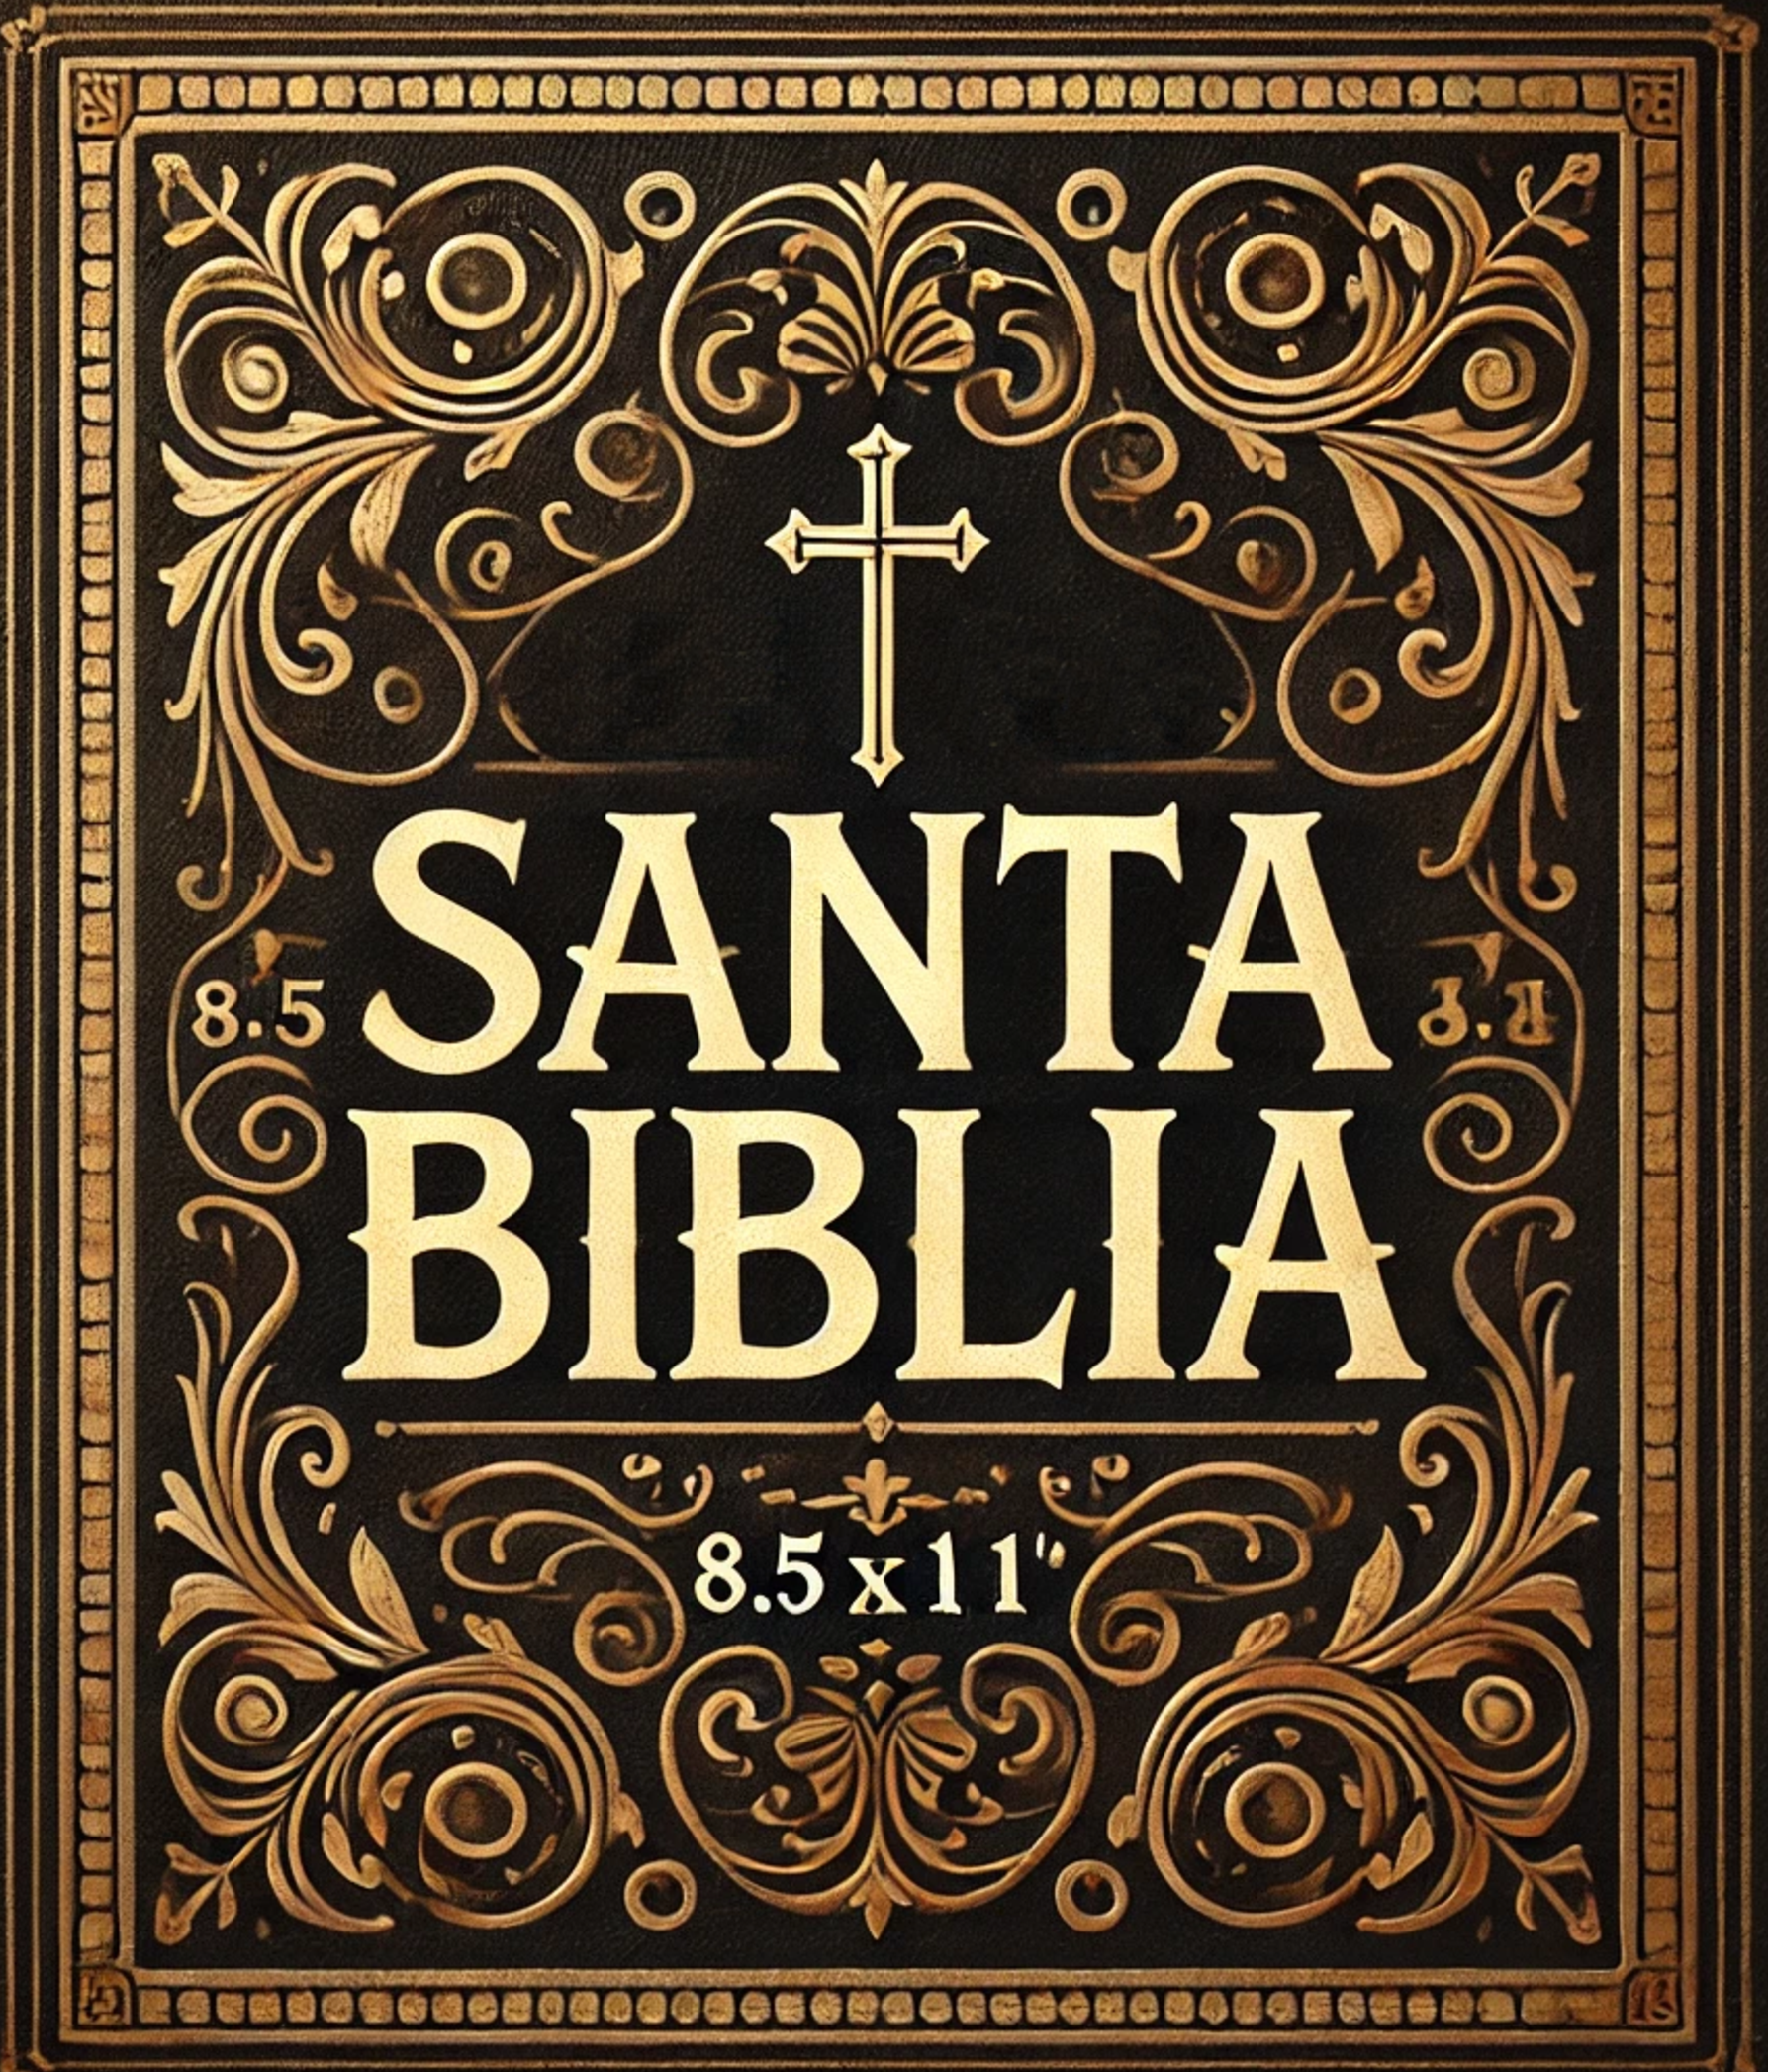
\includegraphics[scale=0.72]{graficas/fondo.pdf}}} % Image background

\vspace*{6cm}
\par\normalfont\fontsize{50}{50}
\begin{flushleft}
%	\textbf{Introducción Redes Complejas}\\
\end{flushleft}

\begin{flushright}
%	{\Large Con Python}
\end{flushright}

{\LARGE }\par % Book title
\vspace*{5cm}
%{\Large  Jorge Mario García Usuga}\par % Author name
%{\Large  Mónica Johana Mesa Mazo}\par % Author name
%{\Large  Valentina Zuluaga Zuluaga}\par % Author name
%{Universidad del Quindío}\par
\endgroup



	
	\frontmatter
	\title{La Biblia}
	\author{Traducida al LaTeX}
	\date{}
	\maketitle
	
	\tableofcontents
	
	\mainmatter
	
	\part{Antiguo Testamento}
	\onecolumn
	
	LA SANTA BIBLIA, ANTIGUO TESTAMENTO, VERSIÓN DE CASIODORO DE REINA (1569)
	REVISADA POR CIPRIANO DE VALERA (1602), OTRAS REVISIONES: 1862, 1909 Y 1960
	
	Parte \# 1 (INCLUYE LA LEY), los 10 primeros libros del AT: Gn, Ex, Lv, Nm, Dt, Jos, Jue, Rt, 1 S y 2 S
	\twocolumn
%	Pentateuco (Ley o Torá)
	
\chapter{Génesis}
%\addcontentsline{toc}{chapter}{Génesis}

\section*{Capítulo 1}
 
La creación  
1:1 En el principio creó Dios los cielos y la tierra.  
1:2 Y la tierra estaba desordenada y vacía, y las tinieblas estaban sobre la faz del abismo, y el Espíritu de Dios se movía sobre la faz de las aguas.  
1:3 Y dijo Dios: Sea la luz;  y fue la luz.  
1:4 Y vio Dios que la luz era buena; y separó Dios la luz de las tinieblas.  
1:5 Y llamó Dios a la luz Día, y a las tinieblas llamó Noche. Y fue la tarde y la mañana un día.  
1:6 Luego dijo Dios: Haya expansión en medio de las aguas, y separe las aguas de las aguas.  
1:7 E hizo Dios la expansión, y separó las aguas que estaban debajo de la expansión, de las aguas que estaban sobre la expansión. Y fue así. 
1:8 Y llamó Dios a la expansión Cielos. Y fue la tarde y la mañana el día segundo.  
1:9 Dijo también Dios: Júntense las aguas que están debajo de los cielos en un lugar, y descúbrase lo seco. Y fue así. 
1:10 Y llamó Dios a lo seco Tierra, y a la reunión de las aguas llamó Mares. Y vio Dios que era bueno.  
1:11 Después dijo Dios: Produzca la tierra hierba verde, hierba que dé semilla; árbol de fruto que dé fruto según su género, que su semilla esté en él, sobre la tierra. Y fue así.  
1:12 Produjo, pues, la tierra hierba verde, hierba que da semilla según su naturaleza, y árbol que da fruto, cuya semilla está en él, según su género. Y vio Dios que era bueno.  
1:13 Y fue la tarde y la mañana el día tercero.  
1:14 Dijo luego Dios: Haya lumbreras en la expansión de los cielos para separar el día de la noche; y sirvan de señales para las estaciones, para días y años,  
1:15 y sean por lumbreras en la expansión de los cielos para alumbrar sobre la tierra. Y fue así.  
1:16 E hizo Dios las dos grandes lumbreras; la lumbrera mayor para que señorease en el día, y la lumbrera menor para que señorease en la noche; hizo también las estrellas.  
1:17 Y las puso Dios en la expansión de los cielos para alumbrar sobre la tierra,  
1:18 y para señorear en el día y en la noche, y para separar la luz de las tinieblas. Y vio Dios que era bueno.  
1:19 Y fue la tarde y la mañana el día cuarto.  
1:20 Dijo Dios: Produzcan las aguas seres vivientes, y aves que vuelen sobre la tierra, en la abierta expansión de los cielos.  
1:21 Y creó Dios los grandes monstruos marinos, y todo ser viviente que se mueve, que las aguas produjeron según su género, y toda ave alada según su especie. Y vio Dios que era bueno.  
1:22 Y Dios los bendijo, diciendo: Fructificad y multiplicaos, y llenad las aguas en los mares, y multiplíquense las aves en la tierra.  
1:23 Y fue la tarde y la mañana el día quinto.  
1:24 Luego dijo Dios: Produzca la tierra seres vivientes según su género, bestias y serpientes y animales de la tierra según su especie. Y fue así.  
1:25 E hizo Dios animales de la tierra según su género, y ganado según su género, y todo animal que se arrastra sobre la tierra según su especie. Y vio Dios que era bueno.  
1:26 Entonces dijo Dios: Hagamos al hombre a nuestra imagen, conforme a nuestra semejanza; y señoree en los peces del mar, en las aves de los cielos, en las bestias, en toda la tierra, y en todo animal que se arrastra sobre la tierra.  
1:27 Y creó Dios al hombre a su imagen, a imagen de Dios lo creó; varón y hembra los creó. 
1:28 Y los bendijo Dios, y les dijo: Fructificad y multiplicaos; llenad la tierra, y sojuzgadla, y señoread en los peces del mar, en las aves de los cielos, y en todas las bestias que se mueven sobre la tierra.  
1:29 Y dijo Dios: He aquí que os he dado toda planta que da semilla, que está sobre toda la tierra, y todo árbol en que hay fruto y que da semilla; os serán para comer.  
1:30 Y a toda bestia de la tierra, y a todas las aves de los cielos, y a todo lo que se arrastra sobre la tierra, en que hay vida, toda planta verde les será para comer. Y fue así.  
1:31 Y vio Dios todo lo que había hecho, y he aquí que era bueno en gran manera. Y fue la tarde y la mañana el día sexto. 
 
\section*{Capítulo 2}

2:1 Fueron, pues, acabados los cielos y la tierra, y todo el ejército de ellos.  
2:2 Y acabó Dios en el día séptimo la obra que hizo; y reposó el día séptimo de toda la obra que hizo.  
2:3 Y bendijo Dios al día séptimo, y lo santificó, porque en él reposó de toda la obra que había hecho en la creación.  
El hombre en el huerto del Edén  
2:4 Estos son los orígenes de los cielos y de la tierra cuando fueron creados, el día que Jehová Dios hizo la tierra y los cielos,  
2:5 y toda planta del campo antes que fuese en la tierra, y toda hierba del campo antes que naciese; porque Jehová Dios aún no había hecho llover sobre la tierra, ni había hombre para que labrase la tierra,  
2:6 sino que subía de la tierra un vapor, el cual regaba toda la faz de la tierra.  
2:7 Entonces Jehová Dios formó al hombre del polvo de la tierra, y sopló en su nariz aliento de vida, y fue el hombre un ser viviente. 
2:8 Y Jehová Dios plantó un huerto en Edén, al oriente; y puso allí al hombre que había formado.  
2:9 Y Jehová Dios hizo nacer de la tierra todo árbol delicioso a la vista, y bueno para comer; también el árbol de vida  en medio del huerto, y el árbol de la ciencia del bien y del mal.  
2:10 Y salía de Edén un río para regar el huerto, y de allí se repartía en cuatro brazos.  
2:11 El nombre del uno era Pisón; éste es el que rodea toda la tierra de Havila, donde hay oro;  
2:12 y el oro de aquella tierra es bueno; hay allí también bedelio y ónice.  
2:13 El nombre del segundo río es Gihón; éste es el que rodea toda la tierra de Cus.  
2:14 Y el nombre del tercer río es Hidekel; éste es el que va al oriente de Asiria. Y el cuarto río es el Eufrates.  
2:15 Tomó, pues, Jehová Dios al hombre, y lo puso en el huerto de Edén, para que lo labrara y lo guardase.  
2:16 Y mandó Jehová Dios al hombre, diciendo: De todo árbol del huerto podrás comer;  
2:17 mas del árbol de la ciencia del bien y del mal no comerás; porque el día que de él comieres, ciertamente morirás.  
2:18 Y dijo Jehová Dios: No es bueno que el hombre esté solo; le haré ayuda idónea para él.  
2:19 Jehová Dios formó, pues, de la tierra toda bestia del campo, y toda ave de los cielos, y las trajo a Adán para que viese cómo las había de llamar; y todo lo que Adán llamó a los animales vivientes, ese es su nombre.  
2:20 Y puso Adán nombre a toda bestia y ave de los cielos y a todo ganado del campo; mas para Adán no se halló ayuda idónea para él.  
2:21 Entonces Jehová Dios hizo caer sueño profundo sobre Adán, y mientras éste dormía, tomó una de sus costillas, y cerró la carne en su lugar.  
2:22 Y de la costilla que Jehová Dios tomó del hombre, hizo una mujer, y la trajo al hombre.  
2:23 Dijo entonces Adán: Esto es ahora hueso de mis huesos y carne de mi carne; ésta será llamada Varona, porque del varón fue tomada.  
2:24 Por tanto, dejará el hombre a su padre y a su madre, y se unirá a su mujer, y serán una sola carne.  
2:25 Y estaban ambos desnudos, Adán y su mujer, y no se avergonzaban.  

\section*{Capítulo 3}
Desobediencia del hombre  

3:1 Pero la serpiente  era astuta, más que todos los animales del campo que Jehová Dios había hecho; la cual dijo a la mujer: ¿Conque Dios os ha dicho: No comáis de todo árbol del huerto?  
3:2 Y la mujer respondió a la serpiente: Del fruto de los árboles del huerto podemos comer;  
3:3 pero del fruto del árbol que está en medio del huerto dijo Dios: No comeréis de él, ni le tocaréis, para que no muráis.  
3:4 Entonces la serpiente dijo a la mujer: No moriréis;  
3:5 sino que sabe Dios que el día que comáis de él, serán abiertos vuestros ojos, y seréis como Dios, sabiendo el bien y el mal.  
3:6 Y vio la mujer que el árbol era bueno para comer, y que era agradable a los ojos, y árbol codiciable para alcanzar la sabiduría; y tomó de su fruto, y comió; y dio también a su marido, el cual comió así como ella.  
3:7 Entonces fueron abiertos los ojos de ambos, y conocieron que estaban desnudos; entonces cosieron hojas de higuera, y se hicieron delantales.  
3:8 Y oyeron la voz de Jehová Dios que se paseaba en el huerto, al aire del día; y el hombre y su mujer se escondieron de la presencia de Jehová Dios entre los árboles del huerto.  
3:9 Mas Jehová Dios llamó al hombre, y le dijo: ¿Dónde estás tú?  
3:10 Y él respondió: Oí tu voz en el huerto, y tuve miedo, porque estaba desnudo; y me escondí.  
3:11 Y Dios le dijo: ¿Quién te enseñó que estabas desnudo? ¿Has comido del árbol de que yo te mandé no comieses?  
3:12 Y el hombre respondió: La mujer que me diste por compañera me dio del árbol, y yo comí.  
3:13 Entonces Jehová Dios dijo a la mujer: ¿Qué es lo que has hecho? Y dijo la mujer: La serpiente me engañó, y comí.  
3:14 Y Jehová Dios dijo a la serpiente: Por cuanto esto hiciste, maldita serás entre todas las bestias y entre todos los animales del campo; sobre tu pecho andarás, y polvo comerás todos los días de tu vida.  
3:15 Y pondré enemistad entre ti y la mujer, y entre tu simiente y la simiente suya; ésta te herirá en la cabeza, y tú le herirás en el calcañar.  
3:16 A la mujer dijo: Multiplicaré en gran manera los dolores en tus preñeces; con dolor darás a luz los hijos; y tu deseo será para tu marido, y él se enseñoreará de ti.  
3:17 Y al hombre dijo: Por cuanto obedeciste a la voz de tu mujer, y comiste del árbol de que te mandé diciendo: No comerás de él; maldita será la tierra por tu causa; con dolor comerás de ella todos los días de tu vida.  
3:18 Espinos y cardos te producirá, y comerás plantas del campo.  
3:19 Con el sudor de tu rostro comerás el pan hasta que vuelvas a la tierra, porque de ella fuiste tomado; pues polvo eres, y al polvo volverás.  
3:20 Y llamó Adán el nombre de su mujer, Eva, por cuanto ella era madre de todos los vivientes.  
3:21 Y Jehová Dios hizo al hombre y a su mujer túnicas de pieles, y los vistió.  
3:22 Y dijo Jehová Dios: He aquí el hombre es como uno de nosotros, sabiendo el bien y el mal; ahora, pues, que no alargue su mano, y tome también del árbol de la vida, y coma, y viva para siempre.  
3:23 Y lo sacó Jehová del huerto del Edén, para que labrase la tierra de que fue tomado.  
3:24 Echó, pues, fuera al hombre, y puso al oriente del huerto de Edén querubines, y una espada encendida que se revolvía por todos lados, para guardar el camino del árbol de la vida.  
\section*{Capítulo 4}
Caín y Abel  

4:1 Conoció Adán a su mujer Eva, la cual concibió y dio a luz a Caín, y dijo: Por voluntad de Jehová he adquirido varón.  
4:2 Después dio a luz a su hermano Abel. Y Abel fue pastor de ovejas, y Caín fue labrador de la tierra.  
4:3 Y aconteció andando el tiempo, que Caín trajo del fruto de la tierra una ofrenda a Jehová.  
4:4 Y Abel trajo también de los primogénitos de sus ovejas, de lo más gordo de ellas. Y miró Jehová con agrado a Abel y a su ofrenda;  
4:5 pero no miró con agrado a Caín y a la ofrenda suya. Y se ensañó Caín en gran manera, y decayó su semblante.  
4:6 Entonces Jehová dijo a Caín: ¿Por qué te has ensañado, y por qué ha decaído tu semblante?  
4:7 Si bien hicieres, ¿no serás enaltecido? y si no hicieres bien, el pecado está a la puerta; con todo esto, a ti será su deseo, y tú te enseñorearás de él.  
4:8 Y dijo Caín a su hermano Abel: Salgamos al campo. Y aconteció que estando ellos en el campo, Caín se levantó contra su hermano Abel, y lo mató.  
4:9 Y Jehová dijo a Caín: ¿Dónde está Abel tu hermano? Y él respondió: No sé. ¿Soy yo acaso guarda de mi hermano?  
4:10 Y él le dijo: ¿Qué has hecho? La voz de la sangre de tu hermano clama a mí desde la tierra.  
4:11 Ahora, pues, maldito seas tú de la tierra, que abrió su boca para recibir de tu mano la sangre de tu hermano.  
4:12 Cuando labres la tierra, no te volverá a dar su fuerza; errante y extranjero serás en la tierra.  
4:13 Y dijo Caín a Jehová: Grande es mi castigo para ser soportado.  
4:14 He aquí me echas hoy de la tierra, y de tu presencia me esconderé, y seré errante y extranjero en la tierra; y sucederá que cualquiera que me hallare, me matará.  
4:15 Y le respondió Jehová: Ciertamente cualquiera que matare a Caín, siete veces será castigado. Entonces Jehová puso señal en Caín, para que no lo matase cualquiera que le hallara.  
4:16 Salió, pues, Caín de delante de Jehová, y habitó en tierra de Nod, al oriente de Edén.  
4:17 Y conoció Caín a su mujer, la cual concibió y dio a luz a Enoc; y edificó una ciudad, y llamó el nombre de la ciudad del nombre de su hijo, Enoc.  
4:18 Y a Enoc le nació Irad, e Irad engendró a Mehujael, y Mehujael engendró a Metusael, y Metusael engendró a Lamec.  
4:19 Y Lamec tomó para sí dos mujeres; el nombre de la una fue Ada, y el nombre de la otra, Zila.  
4:20 Y Ada dio a luz a Jabal, el cual fue padre de los que habitan en tiendas y crían ganados.  
4:21 Y el nombre de su hermano fue Jubal, el cual fue padre de todos los que tocan arpa y flauta.  
4:22 Y Zila también dio a luz a Tubal-caín, artífice de toda obra de bronce y de hierro; y la hermana de Tubal-caín fue Naama.  
4:23 Y dijo Lamec a sus mujeres:  
Ada y Zila, oíd mi voz;  
Mujeres de Lamec, escuchad mi dicho:  
Que un varón mataré por mi herida, 
Y un joven por mi golpe.  
4:24 Si siete veces será vengado Caín,  
Lamec en verdad setenta veces siete lo será. 
4:25 Y conoció de nuevo Adán a su mujer, la cual dio a luz un hijo, y llamó su nombre Set: Porque Dios (dijo ella) me ha sustituido otro hijo en lugar de Abel, a quien mató Caín.  
4:26 Y a Set también le nació un hijo, y llamó su nombre Enós. Entonces los hombres comenzaron a invocar el nombre de Jehová.  


\section*{Capítulo 5}
Los descendientes de Adán  


5:1 Este es el libro de las generaciones de Adán. El día en que creó Dios al hombre, a semejanza de Dios lo hizo.  
5:2 Varón y hembra los creó;  y los bendijo, y llamó el nombre de ellos Adán, el día en que fueron creados.  
5:3 Y vivió Adán ciento treinta años, y engendró un hijo a su semejanza, conforme a su imagen, y llamó su nombre Set.  
5:4 Y fueron los días de Adán después que engendró a Set, ochocientos años, y engendró hijos e hijas.  
5:5 Y fueron todos los días que vivió Adán novecientos treinta años; y murió.  
5:6 Vivió Set ciento cinco años, y engendró a Enós.  
5:7 Y vivió Set, después que engendró a Enós, ochocientos siete años, y engendró hijos e hijas.  
5:8 Y fueron todos los días de Set novecientos doce años; y murió.  
5:9 Vivió Enós noventa años, y engendró a Cainán.  
5:10 Y vivió Enós, después que engendró a Cainán, ochocientos quince años, y engendró hijos e hijas.  
5:11 Y fueron todos los días de Enós novecientos cinco años; y murió.  
5:12 Vivió Cainán setenta años, y engendró a Mahalaleel.  
5:13 Y vivió Cainán, después que engendró a Mahalaleel, ochocientos cuarenta años, y engendró hijos e hijas.  
5:14 Y fueron todos los días de Cainán novecientos diez años; y murió.  
5:15 Vivió Mahalaleel sesenta y cinco años, y engendró a Jared.  
5:16 Y vivió Mahalaleel, después que engendró a Jared, ochocientos treinta años, y engendró hijos e hijas.  
5:17 Y fueron todos los días de Mahalaleel ochocientos noventa y cinco años; y murió.  
5:18 Vivió Jared ciento sesenta y dos años, y engendró a Enoc.  
5:19 Y vivió Jared, después que engendró a Enoc, ochocientos años, y engendró hijos e hijas.  
5:20 Y fueron todos los días de Jared novecientos sesenta y dos años; y murió.  
5:21 Vivió Enoc sesenta y cinco años, y engendró a Matusalén.  
5:22 Y caminó Enoc con Dios, después que engendró a Matusalén, trescientos años, y engendró hijos e hijas.  
5:23 Y fueron todos los días de Enoc trescientos sesenta y cinco años.  
5:24 Caminó, pues, Enoc con Dios, y desapareció, porque le llevó Dios.  
5:25 Vivió Matusalén ciento ochenta y siete años, y engendró a Lamec.  
5:26 Y vivió Matusalén, después que engendró a Lamec, setecientos ochenta y dos años, y engendró hijos e hijas. 
5:27 Fueron, pues, todos los días de Matusalén novecientos sesenta y nueve años; y murió.  
5:28 Vivió Lamec ciento ochenta y dos años, y engendró un hijo;  
5:29 y llamó su nombre Noé, diciendo: Este nos aliviará de nuestras obras y del trabajo de nuestras manos, a causa de la tierra que Jehová maldijo.  
5:30 Y vivió Lamec, después que engendró a Noé, quinientos noventa y cinco años, y engendró hijos e hijas.  
5:31 Y fueron todos los días de Lamec setecientos setenta y siete años; y murió.  
5:32 Y siendo Noé de quinientos años, engendró a Sem, a Cam y a Jafet.  
\section*{Capítulo 6}
La maldad de los hombres  

6:1 Aconteció que cuando comenzaron los hombres a multiplicarse sobre la faz de la tierra, y les nacieron hijas,  
6:2 que viendo los hijos de Dios que las hijas de los hombres eran hermosas, tomaron para sí mujeres, escogiendo entre todas.  
6:3 Y dijo Jehová: No contenderá mi espíritu con el hombre para siempre, porque ciertamente él es carne; mas serán sus días ciento veinte años.  
6:4 Había gigantes en la tierra en aquellos días, y también después que se llegaron los hijos de Dios a las hijas de los hombres, y les engendraron hijos. Estos fueron los valientes que desde la antigüedad fueron varones de renombre.  
6:5 Y vio Jehová que la maldad de los hombres era mucha en la tierra, y que todo designio de los pensamientos del corazón de ellos era de continuo solamente el mal.  
6:6 Y se arrepintió Jehová de haber hecho hombre en la tierra, y le dolió en su corazón.  
6:7 Y dijo Jehová: Raeré de sobre la faz de la tierra a los hombres que he creado, desde el hombre hasta la bestia, y hasta el reptil y las aves del cielo; pues me arrepiento de haberlos hecho.  
6:8 Pero Noé halló gracia ante los ojos de Jehová.  
Noé construye el arca  
6:9 Estas son las generaciones de Noé: Noé, varón justo, era perfecto en sus generaciones; con Dios caminó Noé.  
6:10 Y engendró Noé tres hijos: a Sem, a Cam y a Jafet.  
6:11 Y se corrompió la tierra delante de Dios, y estaba la tierra llena de violencia.  
6:12 Y miró Dios la tierra, y he aquí que estaba corrompida; porque toda carne había corrompido su camino sobre la tierra.  
6:13 Dijo, pues, Dios a Noé: He decidido el fin de todo ser, porque la tierra está llena de violencia a causa de ellos; y he aquí que yo los destruiré con la tierra.  
6:14 Hazte un arca de madera de gofer; harás aposentos en el arca, y la calafatearás con brea por dentro y por fuera.  
6:15 Y de esta manera la harás: de trescientos codos  la longitud del arca, de cincuenta codos su anchura, y de treinta codos su altura.  
6:16 Una ventana harás al arca, y la acabarás a un codo  de elevación por la parte de arriba; y pondrás la puerta del arca a su lado; y le harás piso bajo, segundo y tercero.  
6:17 Y he aquí que yo traigo un diluvio de aguas sobre la tierra, para destruir toda carne en que haya espíritu de vida debajo del cielo; todo lo que hay en la tierra morirá.  
6:18 Mas estableceré mi pacto contigo, y entrarás en el arca tú, tus hijos, tu mujer, y las mujeres de tus hijos contigo.  
6:19 Y de todo lo que vive, de toda carne, dos de cada especie meterás en el arca, para que tengan vida contigo; macho y hembra serán.  
6:20 De las aves según su especie, y de las bestias según su especie, de todo reptil de la tierra según su especie, dos de cada especie entrarán contigo, para que tengan vida.  
6:21 Y toma contigo de todo alimento que se come, y almacénalo, y servirá de sustento para ti y para ellos.  
6:22 Y lo hizo así Noé; hizo conforme a todo lo que Dios le mandó.  
\section*{Capítulo 7}
El diluvio  

7:1 Dijo luego Jehová a Noé: Entra tú y toda tu casa en el arca; porque a ti he visto justo delante de mí en esta generación.  
7:2 De todo animal limpio tomarás siete parejas, macho y su hembra; mas de los animales que no son limpios, una pareja, el macho y su hembra.  
7:3 También de las aves de los cielos, siete parejas, macho y hembra, para conservar viva la especie sobre la faz de la tierra.  
7:4 Porque pasados aún siete días, yo haré llover sobre la tierra cuarenta días y cuarenta noches; y raeré de sobre la faz de la tierra a todo ser viviente que hice.  
7:5 E hizo Noé conforme a todo lo que le mandó Jehová.  
7:6 Era Noé de seiscientos años cuando el diluvio de las aguas vino sobre la tierra.  
7:7 Y por causa de las aguas del diluvio entró Noé al arca, y con él sus hijos, su mujer, y las mujeres de sus hijos.  
7:8 De los animales limpios, y de los animales que no eran limpios, y de las aves, y de todo lo que se arrastra sobre la tierra,  
7:9 de dos en dos entraron con Noé en el arca; macho y hembra, como mandó Dios a Noé.  
7:10 Y sucedió que al séptimo día las aguas del diluvio vinieron sobre la tierra.  
7:11 El año seiscientos de la vida de Noé, en el mes segundo, a los diecisiete días del mes, aquel día fueron rotas todas las fuentes del grande abismo, y las cataratas de los cielos fueron abiertas,  
7:12 y hubo lluvia sobre la tierra cuarenta días y cuarenta noches.  
7:13 En este mismo día entraron Noé, y Sem, Cam y Jafet hijos de Noé, la mujer de Noé, y las tres mujeres de sus hijos, con él en el arca;  
7:14 ellos, y todos los animales silvestres según sus especies, y todos los animales domesticados según sus especies, y todo reptil que se arrastra sobre la tierra según su especie, y toda ave según su especie, y todo pájaro de toda especie.  
7:15 Vinieron, pues, con Noé al arca, de dos en dos de toda carne en que había espíritu de vida.  
7:16 Y los que vinieron, macho y hembra de toda carne vinieron, como le había mandado Dios; y Jehová le cerró la puerta.  
7:17 Y fue el diluvio cuarenta días sobre la tierra; y las aguas crecieron, y alzaron el arca, y se elevó sobre la tierra.  
7:18 Y subieron las aguas y crecieron en gran manera sobre la tierra; y flotaba el arca sobre la superficie de las aguas.  
7:19 Y las aguas subieron mucho sobre la tierra; y todos los montes altos que había debajo de todos los cielos, fueron cubiertos.  
7:20 Quince codos  más alto subieron las aguas, después que fueron cubiertos los montes.  
7:21 Y murió toda carne que se mueve sobre la tierra, así de aves como de ganado y de bestias, y de todo reptil que se arrastra sobre la tierra, y todo hombre.  
7:22 Todo lo que tenía aliento de espíritu de vida en sus narices, todo lo que había en la tierra, murió.  
7:23 Así fue destruido todo ser que vivía sobre la faz de la tierra, desde el hombre hasta la bestia, los reptiles, y las aves del cielo; y fueron raídos de la tierra, y quedó solamente Noé, y los que con él estaban en el arca.  
7:24 Y prevalecieron las aguas sobre la tierra ciento cincuenta días.  
\section*{Capítulo 8}

8:1 Y se acordó Dios de Noé, y de todos los animales, y de todas las bestias que estaban con él en el arca; e hizo pasar Dios un viento sobre la tierra, y disminuyeron las aguas.  
8:2 Y se cerraron las fuentes del abismo y las cataratas de los cielos; y la lluvia de los cielos fue detenida.  
8:3 Y las aguas decrecían gradualmente de sobre la tierra; y se retiraron las aguas al cabo de ciento cincuenta días.  
8:4 Y reposó el arca en el mes séptimo, a los diecisiete días del mes, sobre los montes de Ararat.  
8:5 Y las aguas fueron decreciendo hasta el mes décimo; en el décimo, al primero del mes, se descubrieron las cimas de los montes.  
8:6 Sucedió que al cabo de cuarenta días abrió Noé la ventana del arca que había hecho,  
8:7 y envió un cuervo, el cual salió, y estuvo yendo y volviendo hasta que las aguas se secaron sobre la tierra.  
8:8 Envió también de sí una paloma, para ver si las aguas se habían retirado de sobre la faz de la tierra.  
8:9 Y no halló la paloma donde sentar la planta de su pie, y volvió a él al arca, porque las aguas estaban aún sobre la faz de toda la tierra. Entonces él extendió su mano, y tomándola, la hizo entrar consigo en el arca.  
8:10 Esperó aún otros siete días, y volvió a enviar la paloma fuera del arca.  
8:11 Y la paloma volvió a él a la hora de la tarde; y he aquí que traía una hoja de olivo en el pico; y entendió Noé que las aguas se habían retirado de sobre la tierra.  
8:12 Y esperó aún otros siete días, y envió la paloma, la cual no volvió ya más a él.  
8:13 Y sucedió que en el año seiscientos uno de Noé, en el mes primero, el día primero del mes, las aguas se secaron sobre la tierra; y quitó Noé la cubierta del arca, y miró, y he aquí que la faz de la tierra estaba seca.  
8:14 Y en el mes segundo, a los veintisiete días del mes, se secó la tierra.  
8:15 Entonces habló Dios a Noé, diciendo:  
8:16 Sal del arca tú, y tu mujer, y tus hijos, y las mujeres de tus hijos contigo.  
8:17 Todos los animales que están contigo de toda carne, de aves y de bestias y de todo reptil que se arrastra sobre la tierra, sacarás contigo; y vayan por la tierra, y fructifiquen y multiplíquense sobre la tierra.  
8:18 Entonces salió Noé, y sus hijos, su mujer, y las mujeres de sus hijos con él.  
8:19 Todos los animales, y todo reptil y toda ave, todo lo que se mueve sobre la tierra según sus especies, salieron del arca.  
8:20 Y edificó Noé un altar a Jehová, y tomó de todo animal limpio y de toda ave limpia, y ofreció holocausto en el altar.  
8:21 Y percibió Jehová olor grato; y dijo Jehová en su corazón: No volveré más a maldecir la tierra por causa del hombre; porque el intento del corazón del hombre es malo desde su juventud; ni volveré más a destruir todo ser viviente, como he hecho.  
8:22 Mientras la tierra permanezca, no cesarán la sementera y la siega, el frío y el calor, el verano y el invierno, y el día y la noche.  
\section*{Capítulo 9}
Pacto de Dios con Noé  

9:1 Bendijo Dios a Noé y a sus hijos, y les dijo: Fructificad y multiplicaos, y llenad la tierra. 
9:2 El temor y el miedo de vosotros estarán sobre todo animal de la tierra, y sobre toda ave de los cielos, en todo lo que se mueva sobre la tierra, y en todos los peces del mar; en vuestra mano son entregados.  
9:3 Todo lo que se mueve y vive, os será para mantenimiento: así como las legumbres y plantas verdes, os lo he dado todo.  
9:4 Pero carne con su vida, que es su sangre, no comeréis.  
9:5 Porque ciertamente demandaré la sangre de vuestras vidas; de mano de todo animal la demandaré, y de mano del hombre; de mano del varón su hermano demandaré la vida del hombre.  
9:6 El que derramare sangre de hombre, por el hombre su sangre será derramada; porque a imagen de Dios es hecho el hombre. 
9:7 Mas vosotros fructificad y multiplicaos; procread abundantemente en la tierra, y multiplicaos en ella.  
9:8 Y habló Dios a Noé y a sus hijos con él, diciendo:  
9:9 He aquí que yo establezco mi pacto con vosotros, y con vuestros descendientes después de vosotros;  
9:10 y con todo ser viviente que está con vosotros; aves, animales y toda bestia de la tierra que está con vosotros, desde todos los que salieron del arca hasta todo animal de la tierra.  
9:11 Estableceré mi pacto con vosotros, y no exterminaré ya más toda carne con aguas de diluvio, ni habrá más diluvio para destruir la tierra.  
9:12 Y dijo Dios: Esta es la señal del pacto que yo establezco entre mí y vosotros y todo ser viviente que está con vosotros, por siglos perpetuos:  
9:13 Mi arco he puesto en las nubes, el cual será por señal del pacto entre mí y la tierra.  
9:14 Y sucederá que cuando haga venir nubes sobre la tierra, se dejará ver entonces mi arco en las nubes.  
9:15 Y me acordaré del pacto mío, que hay entre mí y vosotros y todo ser viviente de toda carne; y no habrá más diluvio de aguas para destruir toda carne.  
9:16 Estará el arco en las nubes, y lo veré, y me acordaré del pacto perpetuo entre Dios y todo ser viviente, con toda carne que hay sobre la tierra. 
9:17 Dijo, pues, Dios a Noé: Esta es la señal del pacto que he establecido entre mí y toda carne que está sobre la tierra.  
Embriaguez de Noé  
9:18 Y los hijos de Noé que salieron del arca fueron Sem, Cam y Jafet; y Cam es el padre de Canaán.  
9:19 Estos tres son los hijos de Noé, y de ellos fue llena toda la tierra.  
9:20 Después comenzó Noé a labrar la tierra, y plantó una viña;  
9:21 y bebió del vino, y se embriagó, y estaba descubierto en medio de su tienda.  
9:22 Y Cam, padre de Canaán, vio la desnudez de su padre, y lo dijo a sus dos hermanos que estaban afuera.  
9:23 Entonces Sem y Jafet tomaron la ropa, y la pusieron sobre sus propios hombros, y andando hacia atrás, cubrieron la desnudez de su padre, teniendo vueltos sus rostros, y así no vieron la desnudez de su padre.  
9:24 Y despertó Noé de su embriaguez, y supo lo que le había hecho su hijo más joven,  
9:25 y dijo:  
Maldito sea Canaán;  
Siervo de siervos será a sus hermanos.  
9:26 Dijo más:  
Bendito por Jehová mi Dios sea Sem,  
Y sea Canaán su siervo.  
9:27 Engrandezca Dios a Jafet,  
Y habite en las tiendas de Sem,  
Y sea Canaán su siervo.  
9:28 Y vivió Noé después del diluvio trescientos cincuenta años.  
9:29 Y fueron todos los días de Noé novecientos cincuenta años; y murió. 
\section*{Capítulo 10}
Los descendientes de los hijos de Noé  

10:1 Estas son las generaciones de los hijos de Noé: Sem, Cam y Jafet, a quienes nacieron hijos después del diluvio.  
10:2 Los hijos de Jafet: Gomer, Magog, Madai, Javán, Tubal, Mesec y Tiras.  
10:3 Los hijos de Gomer: Askenaz, Rifat y Togarma.  
10:4 Los hijos de Javán: Elisa, Tarsis, Quitim y Dodanim.  
10:5 De éstos se poblaron las costas, cada cual según su lengua, conforme a sus familias en sus naciones.  
10:6 Los hijos de Cam: Cus, Mizraim, Fut y Canaán.  
10:7 Y los hijos de Cus: Seba, Havila, Sabta, Raama y Sabteca. Y los hijos de Raama: Seba y Dedán.  
10:8 Y Cus engendró a Nimrod, quien llegó a ser el primer poderoso en la tierra.  
10:9 Este fue vigoroso cazador delante de Jehová; por lo cual se dice: Así como Nimrod, vigoroso cazador delante de Jehová.  
10:10 Y fue el comienzo de su reino Babel, Erec, Acad y Calne, en la tierra de Sinar.  
10:11 De esta tierra salió para Asiria, y edificó Nínive, Rehobot, Cala,  
10:12 y Resén entre Nínive y Cala, la cual es ciudad grande.  
10:13 Mizraim engendró a Ludim, a Anamim, a Lehabim, a Naftuhim,  
10:14 a Patrusim, a Casluhim, de donde salieron los filisteos, y a Caftorim.  
10:15 Y Canaán engendró a Sidón su primogénito, a Het,  
10:16 al jebuseo, al amorreo, al gergeseo,  
10:17 al heveo, al araceo, al sineo,  
10:18 al arvadeo, al zemareo y al hamateo; y después se dispersaron las familias de los cananeos.  
10:19 Y fue el territorio de los cananeos desde Sidón, en dirección a Gerar, hasta Gaza; y en dirección de Sodoma, Gomorra, Adma y Zeboim, hasta Lasa.  
10:20 Estos son los hijos de Cam por sus familias, por sus lenguas, en sus tierras, en sus naciones. 
10:21 También le nacieron hijos a Sem, padre de todos los hijos de Heber, y hermano mayor de Jafet.  
10:22 Los hijos de Sem fueron Elam, Asur, Arfaxad, Lud y Aram.  
10:23 Y los hijos de Aram: Uz, Hul, Geter y Mas.  
10:24 Arfaxad engendró a Sala, y Sala engendró a Heber.  
10:25 Y a Heber nacieron dos hijos: el nombre del uno fue Peleg, porque en sus días fue repartida la tierra; y el nombre de su hermano, Joctán.  
10:26 Y Joctán engendró a Almodad, Selef, Hazar-mavet, Jera,  
10:27 Adoram, Uzal, Dicla,  
10:28 Obal, Abimael, Seba,  
10:29 Ofir, Havila y Jobab; todos estos fueron hijos de Joctán.  
10:30 Y la tierra en que habitaron fue desde Mesa en dirección de Sefar, hasta la región montañosa del oriente.  
10:31 Estos fueron los hijos de Sem por sus familias, por sus lenguas, en sus tierras, en sus naciones.  
10:32 Estas son las familias de los hijos de Noé por sus descendencias, en sus naciones; y de éstos se esparcieron las naciones en la tierra después del diluvio. 
\section*{Capítulo 11 }
La torre de Babel  

11:1 Tenía entonces toda la tierra una sola lengua y unas mismas palabras.  
11:2 Y aconteció que cuando salieron de oriente, hallaron una llanura en la tierra de Sinar, y se estabecieron allí.  
11:3 Y se dijeron unos a otros: Vamos, hagamos ladrillo y cozámoslo con fuego. Y les sirvió el ladrillo en lugar de piedra, y el asfalto en lugar de mezcla.  
11:4 Y dijeron: Vamos, edifiquémonos una ciudad y una torre, cuya cúspide llegue al cielo; y hagámonos un nombre, por si fuéremos esparcidos sobre la faz de toda la tierra.  
11:5 Y descendió Jehová para ver la ciudad y la torre que edificaban los hijos de los hombres.  
11:6 Y dijo Jehová: He aquí el pueblo es uno, y todos éstos tienen un solo lenguaje; y han comenzado la obra, y nada les hará desistir ahora de lo que han pensado hacer.  
11:7 Ahora, pues, descendamos, y confundamos allí su lengua, para que ninguno entienda el habla de su compañero.  
11:8 Así los esparció Jehová desde allí sobre la faz de toda la tierra, y dejaron de edificar la ciudad.  
11:9 Por esto fue llamado el nombre de ella Babel, porque allí confundió Jehová el lenguaje de toda la tierra, y desde allí los esparció sobre la faz de toda la tierra.  
Los descendientes de Sem  

11:10 Estas son las generaciones de Sem: Sem, de edad de cien años, engendró a Arfaxad, dos años después del diluvio.  
11:11 Y vivió Sem, después que engendró a Arfaxad, quinientos años, y engendró hijos e hijas.  
11:12 Arfaxad vivió treinta y cinco años, y engendró a Sala.  
11:13 Y vivió Arfaxad, después que engendró a Sala, cuatrocientos tres años, y engendró hijos e hijas.  
11:14 Sala vivió treinta años, y engendró a Heber.  
11:15 Y vivió Sala, después que engendró a Heber, cuatrocientos tres años, y engendró hijos e hijas.  
11:16 Heber vivió treinta y cuatro años, y engendró a Peleg.  
11:17 Y vivió Heber, después que engendró a Peleg, cuatrocientos treinta años, y engendró hijos e hijas.  
11:18 Peleg vivió treinta años, y engendró a Reu.  
11:19 Y vivió Peleg, después que engendró a Reu, doscientos nueve años, y engendró hijos e hijas.  
11:20 Reu vivió treinta y dos años, y engendró a Serug.  
11:21 Y vivió Reu, después que engendró a Serug, doscientos siete años, y engendró hijos e hijas.  
11:22 Serug vivió treinta años, y engendró a Nacor.  
11:23 Y vivió Serug, después que engendró a Nacor, doscientos años, y engendró hijos e hijas.  
11:24 Nacor vivió veintinueve años, y engendró a Taré.  
11:25 Y vivió Nacor, después que engendró a Taré, ciento diecinueve años, y engendró hijos e hijas.  
11:26 Taré vivió setenta años, y engendró a Abram, a Nacor y a Harán.  
Los descendientes de Taré  
11:27 Estas son las generaciones de Taré: Taré engendró a Abram, a Nacor y a Harán; y Harán engendró a Lot.  
11:28 Y murió Harán antes que su padre Taré en la tierra de su nacimiento, en Ur de los caldeos.  
11:29 Y tomaron Abram y Nacor para sí mujeres; el nombre de la mujer de Abram era Sarai, y el nombre de la mujer de Nacor, Milca, hija de Harán, padre de Milca y de Isca.  
11:30 Mas Sarai era estéril, y no tenía hijo.  
11:31 Y tomó Taré a Abram su hijo, y a Lot hijo de Harán, hijo de su hijo, y a Sarai su nuera, mujer de Abram su hijo, y salió con ellos de Ur de los caldeos, para ir a la tierra de Canaán; y vinieron hasta Harán, y se quedaron allí.  
11:32 Y fueron los días de Taré doscientos cinco años; y murió Taré en Harán.  
\section*{Capítulo 12}
Dios llama a Abram  

12:1 Pero Jehová había dicho a Abram: Vete de tu tierra y de tu parentela, y de la casa de tu padre, a la tierra que te mostraré.  
12:2 Y haré de ti una nación grande, y te bendeciré, y engrandeceré tu nombre, y serás bendición.  
12:3 Bendeciré a los que te bendijeren, y a los que te maldijeren maldeciré; y serán benditas en ti todas las familias de la tierra.  
12:4 Y se fue Abram, como Jehová le dijo; y Lot fue con él. Y era Abram de edad de setenta y cinco años cuando salió de Harán.  
12:5 Tomó, pues, Abram a Sarai su mujer, y a Lot hijo de su hermano, y todos sus bienes que habían ganado y las personas que habían adquirido en Harán, y salieron para ir a tierra de Canaán; y a tierra de Canaán llegaron.  
12:6 Y pasó Abram por aquella tierra hasta el lugar de Siquem, hasta el encino de More; y el cananeo estaba entonces en la tierra.  
12:7 Y apareció Jehová a Abram, y le dijo: A tu descendencia daré esta tierra.  Y edificó allí un altar a Jehová, quien le había aparecido.  
12:8 Luego se pasó de allí a un monte al oriente de Bet-el, y plantó su tienda, teniendo a Bet-el al occidente y Hai al oriente; y edificó allí altar a Jehová, e invocó el nombre de Jehová.  
12:9 Y Abram partió de allí, caminando y yendo hacia el Neguev.  
Abram en Egipto  
12:10 Hubo entonces hambre en la tierra, y descendió Abram a Egipto para morar allá; porque era grande el hambre en la tierra.  
12:11 Y aconteció que cuando estaba para entrar en Egipto, dijo a Sarai su mujer: He aquí, ahora conozco que eres mujer de hermoso aspecto;  
12:12 y cuando te vean los egipcios, dirán: Su mujer es; y me matarán a mí, y a ti te reservarán la vida.  
12:13 Ahora, pues, di que eres mi hermana,  para que me vaya bien por causa tuya, y viva mi alma por causa de ti.  
12:14 Y aconteció que cuando entró Abram en Egipto, los egipcios vieron que la mujer era hermosa en gran manera.  
12:15 También la vieron los príncipes de Faraón, y la alabaron delante de él; y fue llevada la mujer a casa de Faraón.  
12:16 E hizo bien a Abram por causa de ella; y él tuvo ovejas, vacas, asnos, siervos, criadas, asnas y camellos.  
12:17 Mas Jehová hirió a Faraón y a su casa con grandes plagas, por causa de Sarai mujer de Abram.  
12:18 Entonces Faraón llamó a Abram, y le dijo: ¿Qué es esto que has hecho conmigo? ¿Por qué no me declaraste que era tu mujer?  
12:19 ¿Por qué dijiste: Es mi hermana, poniéndome en ocasión de tomarla para mí por mujer? Ahora, pues, he aquí tu mujer; tómala, y vete.  
12:20 Entonces Faraón dio orden a su gente acerca de Abram; y le acompañaron, y a su mujer, con todo lo que tenía.  
\section*{Capítulo 13}
Abram y Lot se separan  

13:1 Subió, pues, Abram de Egipto hacia el Neguev, él y su mujer, con todo lo que tenía, y con él Lot.  
13:2 Y Abram era riquísimo en ganado, en plata y en oro.  
13:3 Y volvió por sus jornadas desde el Neguev hacia Bet-el, hasta el lugar donde había estado antes su tienda entre Bet-el y Hai,  
13:4 al lugar del altar que había hecho allí antes; e invocó allí Abram el nombre de Jehová.  
13:5 También Lot, que andaba con Abram, tenía ovejas, vacas y tiendas.  
13:6 Y la tierra no era suficiente para que habitasen juntos, pues sus posesiones eran muchas, y no podían morar en un mismo lugar.  
13:7 Y hubo contienda entre los pastores del ganado de Abram y los pastores del ganado de Lot; y el cananeo y el ferezeo habitaban entonces en la tierra.  
13:8 Entonces Abram dijo a Lot: No haya ahora altercado entre nosotros dos, entre mis pastores y los tuyos, porque somos hermanos.  
13:9 ¿No está toda la tierra delante de ti? Yo te ruego que te apartes de mí. Si fueres a la mano izquierda, yo iré a la derecha; y si tú a la derecha, yo iré a la izquierda.  
13:10 Y alzó Lot sus ojos, y vio toda la llanura del Jordán, que toda ella era de riego, como el huerto de Jehová, como la tierra de Egipto en la dirección de Zoar, antes que destruyese Jehová a Sodoma y a Gomorra.  
13:11 Entonces Lot escogió para sí toda la llanura del Jordán; y se fue Lot hacia el oriente, y se apartaron el uno del otro. 
13:12 Abram acampó en la tierra de Canaán, en tanto que Lot habitó en las ciudades de la llanura, y fue poniendo sus tiendas hasta Sodoma.  
13:13 Mas los hombres de Sodoma eran malos y pecadores contra Jehová en gran manera.  
13:14 Y Jehová dijo a Abram, después que Lot se apartó de él: Alza ahora tus ojos, y mira desde el lugar donde estás hacia el norte y el sur, y al oriente y al occidente.  
13:15 Porque toda la tierra que ves, la daré a ti y a tu descendencia para siempre. 
13:16 Y haré tu descendencia como el polvo de la tierra; que si alguno puede contar el polvo de la tierra, también tu descendencia será contada.  
13:17 Levántate, ve por la tierra a lo largo de ella y a su ancho; porque a ti la daré.  
13:18 Abram, pues, removiendo su tienda, vino y moró en el encinar de Mamre, que está en Hebrón, y edificó allí altar a Jehová.  
\section*{Capítulo 14}
Abram liberta a Lot  

14:1 Aconteció en los días de Amrafel rey de Sinar, Arioc rey de Elasar, Quedorlaomer rey de Elam, y Tidal rey de Goim,  
14:2 que éstos hicieron guerra contra Bera rey de Sodoma, contra Birsa rey de Gomorra, contra Sinab rey de Adma, contra Semeber rey de Zeboim, y contra el rey de Bela, la cual es Zoar.  
14:3 Todos éstos se juntaron en el valle de Sidim, que es el Mar Salado.  
14:4 Doce años habían servido a Quedorlaomer, y en el decimotercero se rebelaron.  
14:5 Y en el año decimocuarto vino Quedorlaomer, y los reyes que estaban de su parte, y derrotaron a los refaítas en Astarot Karnaim, a los zuzitas en Ham, a los emitas en Save-quiriataim,  
14:6 y a los horeos en el monte de Seir, hasta la llanura de Parán, que está junto al desierto.  
14:7 Y volvieron y vinieron a En-mispat, que es Cades, y devastaron todo el país de los amalecitas, y también al amorreo que habitaba en Hazezontamar.  
14:8 Y salieron el rey de Sodoma, el rey de Gomorra, el rey de Adma, el rey de Zeboim y el rey de Bela, que es Zoar, y ordenaron contra ellos batalla en el valle de Sidim;  
14:9 esto es, contra Quedorlaomer rey de Elam, Tidal rey de Goim, Amrafel rey de Sinar, y Arioc rey de Elasar; cuatro reyes contra cinco.  
14:10 Y el valle de Sidim estaba lleno de pozos de asfalto; y cuando huyeron el rey de Sodoma y el de Gomorra, algunos cayeron allí; y los demás huyeron al monte.  
14:11 Y tomaron toda la riqueza de Sodoma y de Gomorra, y todas sus provisiones, y se fueron.  
14:12 Tomaron también a Lot, hijo del hermano de Abram, que moraba en Sodoma, y sus bienes, y se fueron.  
14:13 Y vino uno de los que escaparon, y lo anunció a Abram el hebreo, que habitaba en el encinar de Mamre el amorreo, hermano de Escol y hermano de Aner, los cuales eran aliados de Abram.  
14:14 Oyó Abram que su pariente estaba prisionero, y armó a sus criados, los nacidos en su casa, trescientos dieciocho, y los siguió hasta Dan.  
14:15 Y cayó sobre ellos de noche, él y sus siervos, y les atacó, y les fue siguiendo hasta Hoba al norte de Damasco.  
14:16 Y recobró todos los bienes, y también a Lot su pariente y sus bienes, y a las mujeres y demás gente.  
Melquisedec bendice a Abram  
14:17 Cuando volvía de la derrota de Quedorlaomer y de los reyes que con él estaban, salió el rey de Sodoma a recibirlo al valle de Save, que es el Valle del Rey.  
14:18 Entonces Melquisedec, rey de Salem y sacerdote del Dios Altísimo, sacó pan y vino;  
14:19 y le bendijo, diciendo: Bendito sea Abram del Dios Altísimo, creador de los cielos y de la tierra;  
14:20 y bendito sea el Dios Altísimo, que entregó tus enemigos en tu mano. Y le dio Abram los diezmos de todo.  
14:21 Entonces el rey de Sodoma dijo a Abram: Dame las personas, y toma para ti los bienes.  
14:22 Y respondió Abram al rey de Sodoma: He alzado mi mano a Jehová Dios Altísimo, creador de los cielos y de la tierra,  
14:23 que desde un hilo hasta una correa de calzado, nada tomaré de todo lo que es tuyo, para que no digas: Yo enriquecí a Abram;  
14:24 excepto solamente lo que comieron los jóvenes, y la parte de los varones que fueron conmigo, Aner, Escol y Mamre, los cuales tomarán su parte.  
\section*{Capítulo 15}
Dios promete a Abram un hijo  

15:1 Después de estas cosas vino la palabra de Jehová a Abram en visión, diciendo: No temas, Abram; yo soy tu escudo, y tu galardón será sobremanera grande.  
15:2 Y respondió Abram: Señor Jehová, ¿qué me darás, siendo así que ando sin hijo, y el mayordomo de mi casa es ese damasceno Eliezer?  
15:3 Dijo también Abram: Mira que no me has dado prole, y he aquí que será mi heredero un esclavo nacido en mi casa.  
15:4 Luego vino a él palabra de Jehová, diciendo: No te heredará éste, sino un hijo tuyo será el que te heredará.  
15:5 Y lo llevó fuera, y le dijo: Mira ahora los cielos, y cuenta las estrellas, si las puedes contar. Y le dijo: Así será tu descendencia.  
15:6 Y creyó a Jehová, y le fue contado por justicia.  
15:7 Y le dijo: Yo soy Jehová, que te saqué de Ur de los caldeos, para darte a heredar esta tierra.  
15:8 Y él respondió: Señor Jehová, ¿en qué conoceré que la he de heredar?  
15:9 Y le dijo: Tráeme una becerra de tres años, y una cabra de tres años, y un carnero de tres años, una tórtola también, y un palomino.  
15:10 Y tomó él todo esto, y los partió por la mitad, y puso cada mitad una enfrente de la otra; mas no partió las aves.  
15:11 Y descendían aves de rapiña sobre los cuerpos muertos, y Abram las ahuyentaba.  
15:12 Mas a la caída del sol sobrecogió el sueño a Abram, y he aquí que el temor de una grande oscuridad cayó sobre él.  
15:13 Entonces Jehová dijo a Abram: Ten por cierto que tu descendencia morará en tierra ajena, y será esclava allí, y será oprimida cuatrocientos años.  
15:14 Mas también a la nación a la cual servirán, juzgaré yo; y después de esto saldrán con gran riqueza.  
15:15 Y tú vendrás a tus padres en paz, y serás sepultado en buena vejez.  
15:16 Y en la cuarta generación volverán acá; porque aún no ha llegado a su colmo la maldad del amorreo hasta aquí.  
15:17 Y sucedió que puesto el sol, y ya oscurecido, se veía un horno humeando, y una antorcha de fuego que pasaba por entre los animales divididos.  
15:18 En aquel día hizo Jehová un pacto con Abram, diciendo: A tu descendencia daré esta tierra,  desde el río de Egipto hasta el río grande, el río Eufrates;  
15:19 la tierra de los ceneos, los cenezeos, los admoneos,  
15:20 los heteos, los ferezeos, los refaítas,  
15:21 los amorreos, los cananeos, los gergeseos y los jebuseos.  
\section*{Capítulo 16 }
Agar e Ismael  

16:1 Sarai mujer de Abram no le daba hijos; y ella tenía una sierva egipcia, que se llamaba Agar.  
16:2 Dijo entonces Sarai a Abram: Ya ves que Jehová me ha hecho estéril; te ruego, pues, que te llegues a mi sierva; quizá tendré hijos de ella. Y atendió Abram al ruego de Sarai.  
16:3 Y Sarai mujer de Abram tomó a Agar su sierva egipcia, al cabo de diez años que había habitado Abram en la tierra de Canaán, y la dio por mujer a Abram su marido.  
16:4 Y él se llegó a Agar, la cual concibió; y cuando vio que había concebido, miraba con desprecio a su señora.  
16:5 Entonces Sarai dijo a Abram: Mi afrenta sea sobre ti; yo te di mi sierva por mujer, y viéndose encinta, me mira con desprecio; juzgue Jehová entre tú y yo.  
16:6 Y respondió Abram a Sarai: He aquí, tu sierva está en tu mano; haz con ella lo que bien te parezca. Y como Sarai la afligía, ella huyó de su presencia.  
16:7 Y la halló el ángel de Jehová junto a una fuente de agua en el desierto, junto a la fuente que está en el camino de Shur.  
16:8 Y le dijo: Agar, sierva de Sarai, ¿de dónde vienes tú, y a dónde vas? Y ella respondió: Huyo de delante de Sarai mi señora.  
16:9 Y le dijo el ángel de Jehová: Vuélvete a tu señora, y ponte sumisa bajo su mano.  
16:10 Le dijo también el ángel de Jehová: Multiplicaré tanto tu descendencia, que no podrá ser contada a causa de la multitud. 
16:11 Además le dijo el ángel de Jehová: He aquí que has concebido, y darás a luz un hijo, y llamarás su nombre Ismael, porque Jehová ha oído tu aflicción.  
16:12 Y él será hombre fiero; su mano será contra todos, y la mano de todos contra él, y delante de todos sus hermanos habitará.  
16:13 Entonces llamó el nombre de Jehová que con ella hablaba: Tú eres Dios que ve; porque dijo: ¿No he visto también aquí al que me ve? 
16:14 Por lo cual llamó al pozo: Pozo del Viviente-que-me-ve. He aquí está entre Cades y Bered.  
16:15 Y Agar dio a luz un hijo a Abram, y llamó Abram el nombre del hijo que le dio Agar, Ismael.  
16:16 Era Abram de edad de ochenta y seis años, cuando Agar dio a luz a Ismael.  
\section*{Capítulo 17 }
La circuncisión, señal del pacto  

17:1 Era Abram de edad de noventa y nueve años, cuando le apareció Jehová y le dijo: Yo soy el Dios Todopoderoso; anda delante de mí y sé perfecto.  
17:2 Y pondré mi pacto entre mí y ti, y te multiplicaré en gran manera.  
17:3 Entonces Abram se postró sobre su rostro, y Dios habló con él, diciendo:  
17:4 He aquí mi pacto es contigo, y serás padre de muchedumbre de gentes.  
17:5 Y no se llamará más tu nombre Abram, sino que será tu nombre Abraham,  porque te he puesto por padre de muchedumbre de gentes.  
17:6 Y te multiplicaré en gran manera, y haré naciones de ti, y reyes saldrán de ti.  
17:7 Y estableceré mi pacto entre mí y ti, y tu descendencia después de ti en sus generaciones, por pacto perpetuo,  para ser tu Dios, y el de tu descendencia después de ti.  
17:8 Y te daré a ti, y a tu descendencia después de ti, la tierra en que moras, toda la tierra de Canaán en heredad perpetua;  y seré el Dios de ellos.  
17:9 Dijo de nuevo Dios a Abraham: En cuanto a ti, guardarás mi pacto, tú y tu descendencia después de ti por sus generaciones.  
17:10 Este es mi pacto, que guardaréis entre mí y vosotros y tu descendencia después de ti: Será circuncidado todo varón de entre vosotros.  
17:11 Circuncidaréis, pues, la carne de vuestro prepucio, y será por señal del pacto entre mí y vosotros.  
17:12 Y de edad de ocho días será circuncidado todo varón entre vosotros por vuestras generaciones; el nacido en casa, y el comprado por dinero a cualquier extranjero, que no fuere de tu linaje.  
17:13 Debe ser circuncidado el nacido en tu casa, y el comprado por tu dinero; y estará mi pacto en vuestra carne por pacto perpetuo.  
17:14 Y el varón incircunciso, el que no hubiere circuncidado la carne de su prepucio, aquella persona será cortada de su pueblo; ha violado mi pacto.  
17:15 Dijo también Dios a Abraham: A Sarai tu mujer no la llamarás Sarai, mas Sara será su nombre.  
17:16 Y la bendeciré, y también te daré de ella hijo; sí, la bendeciré, y vendrá a ser madre de naciones; reyes de pueblos vendrán de ella.  
17:17 Entonces Abraham se postró sobre su rostro, y se rió, y dijo en su corazón: ¿A hombre de cien años ha de nacer hijo? ¿Y Sara, ya de noventa años, ha de concebir?  
17:18 Y dijo Abraham a Dios: Ojalá Ismael viva delante de ti.  
17:19 Respondió Dios: Ciertamente Sara tu mujer te dará a luz un hijo, y llamarás su nombre Isaac; y confirmaré mi pacto con él como pacto perpetuo para sus descendientes después de él.  
17:20 Y en cuanto a Ismael, también te he oído; he aquí que le bendeciré, y le haré fructificar y multiplicar mucho en gran manera; doce príncipes engendrará, y haré de él una gran nación. 
17:21 Mas yo estableceré mi pacto con Isaac, el que Sara te dará a luz por este tiempo el año que viene.  
17:22 Y acabó de hablar con él, y subió Dios de estar con Abraham.  
17:23 Entonces tomó Abraham a Ismael su hijo, y a todos los siervos nacidos en su casa, y a todos los comprados por su dinero, a todo varón entre los domésticos de la casa de Abraham, y circuncidó la carne del prepucio de ellos en aquel mismo día, como Dios le había dicho.  
17:24 Era Abraham de edad de noventa y nueve años cuando circuncidó la carne de su prepucio.  
17:25 E Ismael su hijo era de trece años, cuando fue circuncidada la carne de su prepucio.  
17:26 En el mismo día fueron circuncidados Abraham e Ismael su hijo.  
17:27 Y todos los varones de su casa, el siervo nacido en casa, y el comprado del extranjero por dinero, fueron circuncidados con él. 

\section*{Capítulo 18}
Promesa del nacimiento de Isaac  

18:1 Después le apareció Jehová en el encinar de Mamre, estando él sentado a la puerta de su tienda en el calor del día.  
18:2 Y alzó sus ojos y miró, y he aquí tres varones que estaban junto a él; y cuando los vio, salió corriendo de la puerta de su tienda a recibirlos, y se postró en tierra,  
18:3 y dijo: Señor, si ahora he hallado gracia en tus ojos, te ruego que no pases de tu siervo.  
18:4 Que se traiga ahora un poco de agua, y lavad vuestros pies; y recostaos debajo de un árbol,  
18:5 y traeré un bocado de pan, y sustentad vuestro corazón, y después pasaréis; pues por eso habéis pasado cerca de vuestro siervo. Y ellos dijeron: Haz así como has dicho. 
18:6 Entonces Abraham fue de prisa a la tienda a Sara, y le dijo: Toma pronto tres medidas  de flor de harina, y amasa y haz panes cocidos debajo del rescoldo.  
18:7 Y corrió Abraham a las vacas, y tomó un becerro tierno y bueno, y lo dio al criado, y éste se dio prisa a prepararlo.  
18:8 Tomó también mantequilla y leche, y el becerro que había preparado, y lo puso delante de ellos; y él se estuvo con ellos debajo del árbol, y comieron.  
18:9 Y le dijeron: ¿Dónde está Sara tu mujer? Y él respondió: Aquí en la tienda.  
18:10 Entonces dijo: De cierto volveré a ti; y según el tiempo de la vida, he aquí que Sara tu mujer tendrá un hijo. Y Sara escuchaba a la puerta de la tienda, que estaba detrás de él.  
18:11 Y Abraham y Sara eran viejos, de edad avanzada; y a Sara le había cesado ya la costumbre de las mujeres.  
18:12 Se rió, pues, Sara entre sí, diciendo: ¿Después que he envejecido tendré deleite, siendo también mi señor  ya viejo?  
18:13 Entonces Jehová dijo a Abraham: ¿Por qué se ha reído Sara dieciendo: ¿Será cierto que he de dar a luz siendo ya vieja?  
18:14 ¿Hay para Dios alguna cosa difícil?  Al tiempo señalado volveré a ti, y según el tiempo de la vida, Sara tendrá un hijo.  
18:15 Entonces Sara negó, diciendo: No me reí; porque tuvo miedo. Y él dijo: No es así, sino que te has reído.  
Abraham intercede por Sodoma  
18:16 Y los varones se levantaron de allí, y miraron hacia Sodoma; y Abraham iba con ellos acompañándolos.  
18:17 Y Jehová dijo: ¿Encubriré yo a Abraham lo que voy a hacer,  
18:18 habiendo de ser Abraham una nación grande y fuerte, y habiendo de ser benditas en él todas las naciones de la tierra?  
18:19 Porque yo sé que mandará a sus hijos y a su casa después de sí, que guarden el camino de Jehová, haciendo justicia y juicio, para que haga venir Jehová sobre Abraham lo que ha hablado acerca de él.  
18:20 Entonces Jehová le dijo: Por cuanto el clamor contra Sodoma y Gomorra se aumenta más y más, y el pecado de ellos se ha agravado en extremo,  
18:21 descenderé ahora, y veré si han consumado su obra según el clamor que ha venido hasta mí; y si no, lo sabré.  
18:22 Y se apartaron de allí los varones, y fueron hacia Sodoma; pero Abraham estaba aún delante de Jehová.  
18:23 Y se acercó Abraham y dijo: ¿Destruirás también al justo con el impío?  
18:24 Quizá haya cincuenta justos dentro de la ciudad: ¿destruirás también y no perdonarás al lugar por amor a los cincuenta justos que estén dentro de él?  
18:25 Lejos de ti el hacer tal, que hagas morir al justo con el impío, y que sea el justo tratado como el impío; nunca tal hagas. El Juez de toda la tierra, ¿no ha de hacer lo que es justo?  
18:26 Entonces respondió Jehová: Si hallare en Sodoma cincuenta justos dentro de la ciudad, perdonaré a todo este lugar por amor a ellos. 
18:27 Y Abraham replicó y dijo: He aquí ahora que he comenzado a hablar a mi Señor, aunque soy polvo y ceniza.  
18:28 Quizá faltarán de cincuenta justos cinco; ¿destruirás por aquellos cinco toda la ciudad? Y dijo: No la destruiré, si hallare allí cuarenta y cinco.  
18:29 Y volvió a hablarle, y dijo: Quizá se hallarán allí cuarenta. Y respondió: No lo haré por amor a los cuarenta.  
18:30 Y dijo: No se enoje ahora mi Señor, si hablare: quizá se hallarán allí treinta. Y respondió: No lo haré si hallare allí treinta.  
18:31 Y dijo: He aquí ahora que he emprendido el hablar a mi Señor: quizá se hallarán allí veinte. No la destruiré, respondió, por amor a los veinte.  
18:32 Y volvió a decir: No se enoje ahora mi Señor, si hablare solamente una vez: quizá se hallarán allí diez. No la destruiré, respondió, por amor a los diez.  
18:33 Y Jehová se fue, luego que acabó de hablar a Abraham; y Abraham volvió a su lugar.  
\section*{Capítulo 19 }
Destrucción de Sodoma y Gomorra  

19:1 Llegaron, pues, los dos ángeles a Sodoma a la caída de la tarde; y Lot estaba sentado a la puerta de Sodoma. Y viéndolos Lot, se levantó a recibirlos, y se inclinó hacia el suelo,  
19:2 y dijo: Ahora, mis señores, os ruego que vengáis a casa de vuestro siervo y os hospedéis, y lavaréis vuestros pies; y por la mañana os levantaréis, y seguiréis vuestro camino. Y ellos respondieron: No, que en la calle nos quedaremos esta noche.  
19:3 Mas él porfió con ellos mucho, y fueron con él, y entraron en su casa; y les hizo banquete, y coció panes sin levadura, y comieron.  
19:4 Pero antes que se acostasen, rodearon la casa los hombres de la ciudad, los varones de Sodoma, todo el pueblo junto, desde el más joven hasta el más viejo.  
19:5 Y llamaron a Lot, y le dijeron: ¿Dónde están los varones que vinieron a ti esta noche? Sácalos, para que los conozcamos.  
19:6 Entonces Lot salió a ellos a la puerta, y cerró la puerta tras sí,  
19:7 y dijo: Os ruego, hermanos míos, que no hagáis tal maldad.  
19:8 He aquí ahora yo tengo dos hijas que no han conocido varón; os las sacaré fuera, y haced de ellas como bien os pareciere; solamente que a estos varones no hagáis nada, pues que vinieron a la sombra de mi tejado.  
19:9 Y ellos respondieron: Quita allá; y añadieron: Vino este extraño para habitar entre nosotros, ¿y habrá de erigirse en juez? Ahora te haremos más mal que a ellos. Y hacían gran violencia al varón, a Lot, y se acercaron para romper la puerta.  
19:10 Entonces los varones alargaron la mano, y metieron a Lot en casa con ellos, y cerraron la puerta.  
19:11 Y a los hombrs que estaban a la puerta de la casa hirieron con ceguera desde el menor hasta el mayor, de manera que se fatigaban buscando la puerta.  
19:12 Y dijeron los varones a Lot: ¿Tienes aquí alguno más? Yernos, y tus hijos y tus hijas, y todo lo que tienes en la ciudad, sácalo de este lugar;  
19:13 porque vamos a destruir este lugar, por cuanto el clamor contra ellos ha subido de punto delante de Jehová; por tanto, Jehová nos ha enviado para destruirlo. 
19:14 Entonces salió Lot y habló a sus yernos, los que habían de tomar sus hijas, y les dijo: Levantaos, salid de este lugar; porque Jehová va a destruir esta ciudad. Mas pareció a sus yernos como que se burlaba.  
19:15 Y al rayar el alba, los ángeles daban prisa a Lot, diciendo: Levántate, toma tu mujer, y tus dos hijas que se hallan aquí, para que no perezcas en el castigo de la ciudad.  
19:16 Y deteniéndose él, los varones asieron de su mano, y de la mano de su mujer y de las manos de sus dos hijas, según la misericordia de Jehová para con él; y lo sacaron y lo pusieron fuera de la ciudad.  
19:17 Y cuando los hubieron llevado fuera, dijeron: Escapa por tu vida; no mires tras ti, ni pares en toda esta llanura; escapa al monte, no sea que perezcas.  
19:18 Pero Lot les dijo: No, yo os ruego, señores míos.  
19:19 He aquí ahora ha hallado vuestro siervo gracia en vuestros ojos, y habéis engrandecido vuestra misericordia que habéis hecho conmigo dándome la vida; mas yo no podré escapar al monte, no sea que me alcance el mal, y muera.  
19:20 He aquí ahora esta ciudad está cerca para huir allá, la cual es pequeña; dejadme escapar ahora allá (¿no es ella pequeña?), y salvaré mi vida.  
19:21 Y le respondió: He aquí he recibido también tu súplica sobre esto, y no destruiré la ciudad de que has hablado.  
19:22 Date prisa, escápate allá; porque nada podré hacer hasta que hayas llegado allí. Por eso fue llamado el nombre de la ciudad, Zoar.  
19:23 El sol salía sobre la tierra, cuando Lot llegó a Zoar.  
19:24 Entonces Jehová hizo llover sobre Sodoma y sobre Gomorra azufre y fuego de parte de Jehová desde los cielos;  
19:25 y destruyó las ciudades, y toda aquella llanura, con todos los moradores de aquellas ciudades, y el fruto de la tierra.  
19:26 Entonces la mujer de Lot miró atrás, a espaldas de él, y se volvió estatua de sal.  
19:27 Y subió Abraham por la mañana al lugar donde había estado delante de Jehová.  
19:28 Y miró hacia Sodoma y Gomorra, y hacia toda la tierra de aquella llanura miró; y he aquí que el humo subía de la tierra como el humo de un horno. 
19:29 Así, cuando destruyó Dios las ciudades de la llanura, Dios se acordó de Abraham, y envió fuera a Lot de en medio de la destrucción, al asolar las ciudades donde Lot estaba.  
19:30 Pero Lot subió de Zoar y moró en el monte, y sus dos hijas con él; porque tuvo miedo de quedarse en Zoar, y habitó en una cueva él y sus dos hijas.  
19:31 Entonces la mayor dijo a la menor: Nuestro padre es viejo, y no queda varón en la tierra que entre a nosotras conforme a la costumbre de toda la tierra. 
19:32 Ven, demos a beber vino a nuestro padre, y durmamos con él, y conservaremos de nuestro padre descendencia.  
19:33 Y dieron a beber vino a su padre aquella noche, y entró la mayor, y durmió con su padre; mas él no sintió cuándo se acostó ella, ni cuándo se levantó.  
19:34 El día siguiente, dijo la mayor a la menor: He aquí, yo dormí la noche pasada con mi padre; démosle a beber vino también esta noche, y entra y duerme con él, para que conservemos de nuestro padre descendencia.  
19:35 Y dieron a beber vino a su padre también aquella noche, y se levantó la menor, y durmió con él; pero él no echó de ver cuándo se acostó ella, ni cuándo se levantó.  
19:36 Y las dos hijas de Lot concibieron de su padre.  
19:37 Y dio a luz la mayor un hijo, y llamó su nombre Moab, el cual es padre de los moabitas hasta hoy.  
19:38 La menor también dio a luz un hijo, y llamó su nombre Ben- ammi, el cual es padre de los amonitas hasta hoy.  
\section*{Capítulo 20}
Abraham y Abimelec  

20:1 De allí partió Abraham a la tierra del Neguev, y acampó entre Cades y Shur, y habitó como forastero en Gerar.  
20:2 Y dijo Abraham de Sara su mujer: Es mi hermana.  Y Abimelec rey de Gerar envió y tomó a Sara. 
20:3 Pero Dios vino a Abimelec en sueños de noche, y le dijo: He aquí, muerto eres, a causa de la mujer que has tomado, la cual es casada con marido.  
20:4 Mas Abimelec no se había llegado a ella, y dijo: Señor, ¿matarás también al inocente?  
20:5 ¿No me dijo él: Mi hermana es; y ella también dijo: Es mi hermano? con sencillez de mi corazón y con limpieza de mis manos he hecho esto.  
20:6 Y le dijo Dios en sueños: Yo también sé que con integridad de tu corazón has hecho esto; y yo también te detuve de pecar contra mí, y así no te permití que la tocases.  
20:7 Ahora, pues, devuelve la mujer a su marido; porque es profeta, y orará por ti, y vivirás. Y si no la devolvieres, sabe que de cierto morirás tú, y todos los tuyos.  
20:8 Entonces Abimelec se levantó de mañana y llamó a todos sus siervos, y dijo todas estas palabras en los oídos de ellos; y temieron los hombres en gran manera.  
20:9 Después llamó Abimelec a Abraham, y le dijo: ¿Qué nos has hecho? ¿En qué pequé yo contra ti, que has atraído sobre mí y sobre mi reino tan grande pecado? Lo que no debiste hacer has hecho conmigo.  
20:10 Dijo también Abimelec a Abraham: ¿Qué pensabas, para que hicieses esto?  
20:11 Y Abraham respondió: Porque dije para mí: Ciertamente no hay temor de Dios en este lugar, y me matarán por causa de mi mujer.  
20:12 Y a la verdad también es mi hermana, hija de mi padre, mas no hija de mi madre, y la tomé por mujer.  
20:13 Y cuando Dios me hizo salir errante de la casa de mi padre, yo le dije: Esta es la merced que tú harás conmigo, que en todos los lugares adonde lleguemos, digas de mí: Mi hermano es.  
20:14 Entonces Abimelec tomó ovejas y vacas, y siervos y siervas, y se los dio a Abraham, y le devolvió a Sara su mujer.  
20:15 Y dijo Abimelec: He aquí mi tierra está delante de ti; habita donde bien te parezca.  
20:16 Y a Sara dijo: He aquí he dado mil monedas de plata a tu hermano; mira que él te es como un velo para los ojos de todos los que están contigo, y para con todos; así fue vindicada.  
20:17 Entonces Abraham oró a Dios; y Dios sanó a Abimelec y a su mujer, y a sus siervas, y tuvieron hijos.  
20:18 Porque Jehová había cerrado completamente toda matriz de la casa de Abimelec, a causa de Sara mujer de Abraham.  
\section*{Capítulo 21}
Nacimiento de Isaac  

21:1 Visitó Jehová a Sara, como había dicho, e hizo Jehová con Sara como había hablado.  
21:2 Y Sara concibió y dio a Abraham un hijo en su vejez, en el tiempo que Dios le había dicho.  
21:3 Y llamó Abraham el nombre de su hijo que le nació, que le dio a luz Sara, Isaac.  
21:4 Y circuncidó Abraham a su hijo Isaac de ocho días, como Dios le había mandado.  
21:5 Y era Abraham de cien años cuando nació Isaac su hijo.  
21:6 Entonces dijo Sara: Dios me ha hecho reir, y cualquiera que lo oyere, se reirá conmigo.  
21:7 Y añadió: ¿Quién dijera a Abraham que Sara habría de dar de mamar a hijos? Pues le he dado un hijo en su vejez.  
Agar e Ismael son echados de la casa de Abraham  
21:8 Y creció el niño, y fue destetado; e hizo Abraham gran banquete el día que fue destetado Isaac.  
21:9 Y vio Sara que el hijo de Agar la egipcia, el cual ésta le había dado a luz a Abraham, se burlaba de su hijo Isaac.  
21:10 Por tanto, dijo a Abraham: Echa a esta sierva y a su hijo, porque el hijo de esta sierva no ha de heredar con Isaac mi hijo.  
21:11 Este dicho pareció grave en gran manera a Abraham a causa de su hijo.  
21:12 Entonces dijo Dios a Abraham: No te parezca grave a causa del muchacho y de tu sierva; en todo lo que te dijere Sara, oye su voz, porque en Isaac te será llamada descendencia.  
21:13 Y también del hijo de la sierva haré una nación, porque es tu descendiente.  
21:14 Entonces Abraham se levantó muy de mañana, y tomó pan, y un odre de agua, y lo dio a Agar, poniéndolo sobre su hombro, y le entregó el muchacho, y la despidió. Y ella salió y anduvo errante por el desierto de Beerseba.  
21:15 Y le faltó el agua del odre, y echó al muchacho debajo de un arbusto,  
21:16 y se fue y se sentó enfrente, a distancia de un tiro de arco; porque decía: No veré cuando el muchacho muera. Y cuando ella se sentó enfrente, el muchacho alzó su voz y lloró. 
21:17 Y oyó Dios la voz del muchacho; y el ángel de Dios llamó a Agar desde el cielo, y le dijo: ¿Qué tienes, Agar? No temas; porque Dios ha oído la voz del muchacho en donde está.  
21:18 Levántate, alza al muchacho, y sostenlo con tu mano, porque yo haré de él una gran nación.  
21:19 Entonces Dios le abrió los ojos, y vio una fuente de agua; y fue y llenó el odre de agua, y dio de beber al muchacho.  
21:20 Y Dios estaba con el muchacho; y creció, y habitó en el desierto, y fue tirador de arco.  
21:21 Y habitó en el desierto de Parán; y su madre le tomó mujer de la tierra de Egipto.  
Pacto entre Abraham y Abimelec  
21:22 Aconteció en aquel mismo tiempo que habló Abimelec, y Ficol príncipe de su ejército, a Abraham, diciendo: Dios está contigo en todo cuanto haces.  
21:23 Ahora, pues, júrame aquí por Dios, que no faltarás a mí, ni a mi hijo ni a mi nieto, sino que conforme a la bondad que yo hice contigo, harás tú conmigo, y con la tierra en donde has morado.  
21:24 Y respondió Abraham: Yo juraré.  
21:25 Y Abraham reconvino a Abimelec a causa de un pozo de agua, que los siervos de Abimelec le habían quitado.  
21:26 Y respondió Abimelec: No sé quién haya hecho esto, ni tampoco tú me lo hiciste saber, ni yo lo he oído hasta hoy.  
21:27 Y tomó Abraham ovejas y vacas, y dio a Abimelec; e hicieron ambos pacto.  
21:28 Entonces puso Abraham siete corderas del rebaño aparte.  
21:29 Y dijo Abimelec a Abraham: ¿Qué significan esas siete corderas que has puesto aparte?  
21:30 Y él respondió: Que estas siete corderas tomarás de mi mano, para que me sirvan de testimonio de que yo cavé este pozo.  
21:31 Por esto llamó a aquel lugar Beerseba; porque allí juraron ambos.  
21:32 Así hicieron pacto en Beerseba; y se levantó Abimelec, y Ficol príncipe de su ejército, y volvieron a tierra de los filisteos.  
21:33 Y plantó Abraham un árbol tamarisco en Beerseba, e invocó allí el nombre de Jehová Dios eterno.  
21:34 Y moró Abraham en tierra de los filisteos muchos días.  
\section*{Capítulo 22}
Dios ordena a Abraham que sacrifique a Isaac  

22:1 Aconteció después de estas cosas, que probó Dios a Abraham, y le dijo: Abraham. Y él respondió: Heme aquí.  
22:2 Y dijo: Toma ahora tu hijo, tu único, Isaac, a quien amas, y vete a tierra de Moriah, y ofrécelo allí en holocausto sobre uno de los montes que yo te diré.  
22:3 Y Abraham se levantó muy de mañana, y enalbardó su asno, y tomó consigo dos siervos suyos, y a Isaac su hijo; y cortó leña para el holocausto, y se levantó, y fue al lugar que Dios le dijo.  
22:4 Al tercer día alzó Abraham sus ojos, y vio el lugar de lejos.  
22:5 Entonces dijo Abraham a sus siervos: Esperad aquí con el asno, y yo y el muchacho iremos hasta allí y adoraremos, y volveremos a vosotros.  
22:6 Y tomó Abraham la leña del holocausto, y la puso sobre Isaac su hijo, y él tomó en su mano el fuego y el cuchillo; y fueron ambos juntos.  
22:7 Entonces habló Isaac a Abraham su padre, y dijo: Padre mío. Y él respondió: Heme aquí, mi hijo. Y él dijo: He aquí el fuego y la leña; mas ¿dónde está el cordero para el holocausto?  
22:8 Y respondió Abraham: Dios se proveerá de cordero para el holocausto, hijo mío. E iban juntos.  
22:9 Y cuando llegaron al lugar que Dios le había dicho, edificó allí Abraham un altar,  y compuso la leña, y ató a Isaac su hijo, y lo puso en el altar sobre la leña.  
22:10 Y extendió Abraham su mano y tomó el cuchillo para degollar a su hijo.  
22:11 Entonces el ángel de Jehová le dio voces desde el cielo, y dijo: Abraham, Abraham. Y él respondió: Heme aquí.  
22:12 Y dijo: No extiendas tu mano sobre el muchacho, ni le hagas nada; porque ya conozco que temes a Dios, por cuanto no me rehusaste tu hijo, tu único.  
22:13 Entonces alzó Abraham sus ojos y miró, y he aquí a sus espaldas un carnero trabado en un zarzal por sus cuernos; y fue Abraham y tomó el carnero, y lo ofreció en holocausto en lugar de su hijo.  
22:14 Y llamó Abraham el nombre de aquel lugar, Jehová proveerá. Por tanto se dice hoy: En el monte de Jehová será provisto.  
22:15 Y llamó el ángel de Jehová a Abraham por segunda vez desde el cielo,  
22:16 y dijo: Por mí mismo he jurado, dice Jehová, que por cuanto has hecho esto, y no me has rehusado tu hijo, tu único hijo;  
22:17 de cierto te bendeciré, y multiplicaré tu descendencia como las estrellas del cielo y como la arena que está a la orilla del mar; y tu descendencia poseerá las puertas de sus enemigos.  
22:18 En tu simiente serán benditas todas las naciones de la tierra, por cuanto obedeciste a mi voz.  
22:19 Y volvió Abraham a sus siervos, y se levantaron y se fueron juntos a Beerseba; y habitó Abraham en Beerseba.  
22:20 Aconteció después de estas cosas, que fue dada noticia a Abraham, diciendo: He aquí que también Milca ha dado a luz hijos a Nacor tu hermano:  
22:21 Uz su primogénito, Buz su hermano, Kemuel padre de Aram,  
22:22 Quesed, Hazo, Pildas, Jidlaf y Betuel.  
22:23 Y Betuel fue el padre de Rebeca. Estos son los ocho hijos que dio a luz Milca, de Nacor hermano de Abraham.  
22:24 Y su concubina, que se llamaba Reúma, dio a luz también a Teba, a Gaham, a Tahas y a Maaca.  
\section*{Capítulo 23}
Muerte y sepultura de Sara  

23:1 Fue la vida de Sara ciento veintisiete años; tantos fueron los años de la vida de Sara.  
23:2 Y murió Sara en Quiriat-arba, que es Hebrón, en la tierra de Canaán; y vino Abraham a hacer duelo por Sara, y a llorarla.  
23:3 Y se levantó Abraham de delante de su muerta, y habló a los hijos de Het, diciendo:  
23:4 Extranjero y forastero soy entre vosotros; dadme propiedad para sepultura entre vosotros, y sepultaré mi muerta de delante de mí.  
23:5 Y respondieron los hijos de Het a Abraham, y le dijeron:  
23:6 Oyenos, señor nuestro; eres un príncipe de Dios entre nosotros; en lo mejor de nuestros sepulcros sepulta a tu muerta; ninguno de nosotros te negará su sepulcro, ni te impedirá que entierres tu muerta.  
23:7 Y Abraham se levantó, y se inclinó al pueblo de aquella tierra, a los hijos de Het,  
23:8 y habló con ellos, diciendo: Si tenéis voluntad de que yo sepulte mi muerta de delante de mí, oídme, e interceded por mí con Efrón hijo de Zohar,  
23:9 para que me dé la cueva de Macpela, que tiene al extremo de su heredad; que por su justo precio me la dé, para posesión de sepultura en medio de vosotros.  
23:10 Este Efrón estaba entre los hijos de Het; y respondió Efrón heteo a Abraham, en presencia de los hijos de Het, de todos los que entraban por la puerta de su ciudad, diciendo:  
23:11 No, señor mío, óyeme: te doy la heredad, y te doy también la cueva que está en ella; en presencia de los hijos de mi pueblo te la doy; sepulta tu muerta.  
23:12 Entonces Abraham se inclinó delante del pueblo de la tierra,  
23:13 y respondió a Efrón en presencia del pueblo de la tierra, deciendo: Antes, si te place, te ruego que me oigas. Yo daré el precio de la heredad; tómalo de mí, y sepultaré en ella mi muerta.  
23:14 Respondió Efrón a Abraham, diciéndole:  
23:15 Señor mío, escúchame: la tierra vale cuatrocientos siclos de plata; ¿qué es esto entre tú y yo? Entierra, pues, tu muerta.  
23:16 Entonces Abraham se convino con Efrón, y pesó Abraham a Efrón el dinero que dijo, en presencia de los hijos de Het, cuatrocientos siclos de plata, de buena ley entre mercaderes.  
23:17 Y quedó la heredad de Efrón que estaba en Macpela al oriente de Mamre, la heredad con la cueva que estaba en ella, y todos los árboles que había en la heredad, y en todos sus contornos,  
23:18 como propiedad de Abraham, en presencia de los hijos de Het y de todos los que entraban por la puerta de la ciudad.  
23:19 Después de esto sepultó Abraham a Sara su mujer en la cueva de la heredad de Macpela al oriente de Mamre, que es Hebrón, en la tierra de Canaán.  
23:20 Y quedó la heredad y la cueva que en ella había, de Abraham, como una posesión para sepultura, recibida de los hijos de Het.  
\section*{Capítulo 24}
Abraham busca esposa para Isaac  

24:1 Era Abraham ya viejo, y bien avanzado en años; y Jehová había bendecido a Abraham en todo.  
24:2 Y dijo Abraham a un criado suyo, el más viejo de su casa, que era el que gobernaba en todo lo que tenía: Pon ahora tu mano debajo de mi muslo,  
24:3 y te juramentaré por Jehová, Dios de los cielos y Dios de la tierra, que no tomarás para mi hijo mujer de las hijas de los cananeos, entre los cuales yo habito; 
24:4 sino que irás a mi tierra y a mi parentela, y tomarás mujer para mi hijo Isaac.  
24:5 El criado le respondió: Quizá la mujer no querrá venir en pos de mí a esta tierra. ¿Volveré, pues, tu hijo a la tierra de donde saliste?  
24:6 Y Abraham le dijo: Guárdate que no vuelvas a mi hijo allá.  
24:7 Jehová, Dios de los cielos, que me tomó de la casa de mi padre y de la tierra de mi parentela, y me habló y me juró, diciendo: A tu descendencia daré esta tierra; él enviará su ángel delante de ti, y tú traerás de allá mujer para mi hijo.  
24:8 Y si la mujer no quisiere venir en pos de ti, serás libre de este mi juramento; solamente que no vuelvas allá a mi hijo.  
24:9 Entonces el criado puso su mano debajo del muslo de Abraham su señor, y le juró sobre este negocio.  
24:10 Y el criado tomó diez camellos de los camellos de su señor, y se fue, tomando toda clase de regalos escogidos de su señor; y puesto en camino, llegó a Mesopotamia, a la ciudad de Nacor.  
24:11 E hizo arrodillar los camellos fuera de la ciudad, junto a un pozo de agua, a la hora de la tarde, la hora en que salen las doncellas por agua.  
24:12 Y dijo: Oh Jehová, Dios de mi señor Abraham, dame, te ruego, el tener hoy buen encuentro, y haz misericordia con mi señor Abraham.  
24:13 He aquí yo estoy junto a la fuente de agua, y las hijas de los varones de esta ciudad salen por agua.  
24:14 Sea, pues, que la doncella a quien yo dijere: Baja tu cántaro, te ruego, para que yo beba, y ella respondiere: Bebe, y también daré de beber a tus camellos; que sea ésta la que tú has destinado para tu siervo Isaac; y en esto conoceré que habrás hecho misericordia con mi señor.  
24:15 Y aconteció que antes que él acabase de hablar, he aquí Rebeca, que había nacido a Betuel, hijo de Milca mujer de Nacor hermano de Abraham, la cual salía con su cántaro sobre su hombro.  
24:16 Y la doncella era de aspecto muy hermoso, virgen, a la que varón no había conocido; la cual descendió a la fuente, y llenó su cántaro, y se volvía.  
24:17 Entonces el criado corrió hacia ella, y dijo: Te ruego que me des a beber un poco de agua de tu cántaro.  
24:18 Ella respondió: Bebe, señor mío; y se dio prisa a bajar su cántaro sobre su mano, y le dio a beber.  
24:19 Y cuando acabó de darle de beber, dijo: También para tus camellos sacaré agua, hasta que acaben de beber.  
24:20 Y se dio prisa, y vació su cántaro en la pila, y corrió otra vez al pozo para sacar agua, y sacó para todos sus camellos.  
24:21 Y el hombre estaba maravillado de ella, callando, para saber si Jehová había prosperado su viaje, o no.  
24:22 Y cuando los camellos acabaron de beber, le dio el hombre un pendiente de oro que pesaba medio siclo, y dos brazaletes que pesaban diez,  
24:23 y dijo: ¿De quién eres hija? Te ruego que me digas: ¿hay en casa de tu padre lugar donde posemos?  
24:24 Y ella respondió: Soy hija de Betuel hijo de Milca, el cual ella dio a luz a Nacor.  
24:25 Y añadió: También hay en nuestra casa paja y mucho forraje, y lugar para posar.  
24:26 El hombre entonces se inclinó, y adoró a Jehová,  
24:27 y dijo: Bendito sea Jehová, Dios de mi amo Abraham, que no apartó de mi amo su misericordia y su verdad, guiándome Jehová en el camino a casa de los hermanos de mi amo.  
24:28 Y la doncella corrió, e hizo saber en casa de su madre estas cosas.  
24:29 Y Rebeca tenía un hermano que se llamaba Labán, el cual corrió afuera hacia el hombre, a la fuente.  
24:30 Y cuando vio el pendiente y los brazaletes en las manos de su hermana, que decía: Así me habló aquel hombre, vino a él; y he aquí que estaba con los camellos junto a la fuente.  
24:31 Y le dijo: Ven, bendito de Jehová; ¿por qué estás fuera? He preparado la casa, y el lugar para los camellos.  
24:32 Entonces el hombre vino a casa, y Labán desató los camellos; y les dio paja y forraje, y agua para lavar los pies de él, y los pies de los hombres que con él venían.  
24:33 Y le pusieron delante qué comer; mas él dijo: No comeré hasta que haya dicho mi mensaje. Y él le dijo: Habla.  
24:34 Entonces dijo: Yo soy criado de Abraham.  
24:35 Y Jehová ha bendecido mucho a mi amo, y él se ha engrandecido; y le ha dado ovejas y vacas, plata y oro, siervos y siervas, camellos y asnos.  
24:36 Y Sara, mujer de mi amo, dio a luz en su vejez un hijo a mi señor, quien le ha dado a él todo cuanto tiene.  
24:37 Y mi amo me hizo jurar, diciendo: No tomarás para mi hijo mujer de las hijas de los cananeos, en cuya tierra habito;  
24:38 sino que irás a la casa de mi padre y a mi parentela, y tomarás mujer para mi hijo.  
24:39 Y yo dije: Quizás la mujer no querrá seguirme.  
24:40 Entonces él me respondió: Jehová, en cuya presencia he andado, enviará su ángel contigo, y prosperará tu camino; y tomarás para mi hijo mujer de mi familia y de la casa de mi padre.  
24:41 Entonces serás libre de mi juramento, cuando hayas llegado a mi familia; y si no te la dieren, serás libre de mi juramento.  
24:42 Llegué, pues, hoy a la fuente, y dije: Jehová, Dios de mi señor Abraham, si tú prosperas ahora mi camino por el cual ando,  
24:43 he aquí yo estoy junto a la fuente de agua; sea, pues, que la doncella que saliere por agua, a la cual dijere: Dame de beber, te ruego, un poco de agua de tu cántaro,  
24:44 y ella me respondiere: Bebe tú, y también para tus camellos sacaré agua; sea ésta la mujer que destinó Jehová para el hijo de mi señor.  
24:45 Antes que acabase de hablar en mi corazón, he aquí Rebeca, que salía con su cántaro sobre su hombro; y descendió a la fuente, y sacó agua; y le dije: te ruego que me des de beber.  
24:46 Y bajó prontamente su cántaro de encima de sí, y dijo: Bebe, y también a tus camellos daré de beber. Y bebí, y dio también de beber a mis camellos.  
24:47 Entonces le pregunté, y dije: ¿De quién eres hija? Y ella respondió: Hija de Betuel hijo de Nacor, que le dio a luz Milca. Entonces le puse un pendiente en su nariz, y brazaletes en sus brazos;  
24:48 y me incliné y adoré a Jehová, y bendije a Jehová Dios de mi señor Abraham, que me había guiado por camino de verdad para tomar la hija del hermano de mi señor para su hijo.  
24:49 Ahora, pues, si vosotros hacéis misericordia y verdad con mi señor, declarádmelo; y si no, declarádmelo; y me iré a la diestra o a la siniestra.  
24:50 Entonces Labán y Betuel respondieron y dijeron: De Jehová ha salido esto; no podemos hablarte malo ni bueno.  
24:51 He ahí Rebeca delante de ti; tómala y vete, y sea mujer del hijo de tu señor, como lo ha dicho Jehová.  
24:52 Cuando el criado de Abraham oyó sus palabras, se inclinó en tierra ante Jehová.  
24:53 Y sacó el criado alhajas de plata y alhajas de oro, y vestidos, y dio a Rebeca; también dio cosas preciosas a su hermano y a su madre.  
24:54 Y comieron y bebieron él y los varones que venían con él, y durmieron; y levantándose de mañana, dijo: Enviadme a mi señor.  
24:55 Entonces respondieron su hermano y su madre: Espere la doncella con nosotros a lo menos diez días, y después irá.  
24:56 Y él les dijo: No me detengáis, ya que Jehová ha prosperado mi camino; despachadme para que me vaya a mi señor.  
24:57 Ellos respondieron entonces: Llamemos a la doncella y preguntémosle.  
24:58 Y llamaron a Rebeca, y le dijeron: ¿Irás tú con este varón? Y ella respondió: Sí, iré.  
24:59 Entonces dejaron ir a Rebeca su hermana, y a su nodriza, y al criado de Abraham y a sus hombres.  
24:60 Y bendijeron a Rebeca, y le dijeron: Hermana nuestra, sé madre de millares de millares, y posean tus descendientes la puerta de sus enemigos.  
24:61 Entonces se levantó Rebeca y sus doncellas, y montaron en los camellos, y siguieron al hombre; y el criado tomó a Rebeca, y se fue.  
24:62 Y venía Isaac del pozo del Viviente-que-me-ve; porque él habitaba en el Neguev.  
24:63 Y había salido Isaac a meditar al campo, a la hora de la tarde; y alzando sus ojos miró, y he aquí los camellos que venían.  
24:64 Rebeca también alzó sus ojos, y vio a Isaac, y descendió del camello;  
24:65 porque había preguntado al criado: ¿Quién es este varón que viene por el campo hacia nosotros? Y el criado había respondido: Este es mi señor. Ella entonces tomó el velo, y se cubrió.  
24:66 Entonces el criado contó a Isaac todo lo que había hecho.  
24:67 Y la trajo Isaac a la tienda de su madre Sara, y tomó a Rebeca por mujer, y la amó; y se consoló Isaac después de la muerte de su madre. 
\section*{Capítulo 25}
Los descendientes de Abraham y Cetura  


25:1 Abraham tomó otra mujer, cuyo nombre era Cetura,  
25:2 la cual le dio a luz a Zimram, Jocsán, Medán, Madián, Isbac y Súa.  
25:3 Y Jocsán engendró a Seba y a Dedán; e hijos de Dedán fueron Asurim, Letusim y Leumim. 
25:4 E hijos de Madián: Efa, Efer, Hanoc, Abida y Elda. Todos estos fueron hijos de Cetura.  
25:5 Y Abraham dio todo cuanto tenía a Isaac.  
25:6 Pero a los hijos de sus concubinas dio Abraham dones, y los envió lejos de Isaac su hijo, mientras él vivía, hacia el oriente, a la tierra oriental.  
Muerte y sepultura de Abraham  
25:7 Y estos fueron los días que vivió Abraham: ciento setenta y cinco años.  
25:8 Y exhaló el espíritu, y murió Abraham en buena vejez, anciano y lleno de años, y fue unido a su pueblo.  
25:9 Y lo sepultaron Isaac e Ismael sus hijos en la cueva de Macpela, en la heredad de Efrón hijo de Zohar heteo, que está enfrente de Mamre,  
25:10 heredad que compró Abraham de los hijos de Het; allí fue sepultado Abraham, y Sara su mujer.  
25:11 Y sucedió, después de muerto Abraham, que Dios bendijo a Isaac su hijo; y habitó Isaac junto al pozo del Viviente-que-me- ve.  
Los descendientes de Ismael  

25:12 Estos son los descendientes de Ismael hijo de Abraham, a quien le dio a luz Agar egipcia, sierva de Sara;  
25:13 estos, pues, son los nombres de los hijos de Ismael, nombrados en el orden de su nacimiento: El primogénito de Ismael, Nebaiot; luego Cedar, Adbeel, Mibsam,  
25:14 Misma, Duma, Massa,  
25:15 Hadar, Tema, Jetur, Nafis y Cedema.  
25:16 Estos son los hijos de Ismael, y estos sus nombres, por sus villas y por sus campamentos; doce príncipes por sus familias.  
25:17 Y estos fueron los años de la vida de Ismael, ciento treinta y siete años; y exhaló el espíritu Ismael, y murió, y fue unido a su pueblo.  
25:18 Y habitaron desde Havila hasta Shur, que está enfrente de Egipto viniendo a Asiria; y murió en presencia de todos sus hermanos.  
Nacimiento de Jacob y Esaú  
25:19 Estos son los descendientes de Isaac hijo de Abraham: Abraham engendró a Isaac,  
25:20 y era Isaac de cuarenta años cuando tomó por mujer a Rebeca, hija de Betuel arameo de Padan-aram, hermana de Labán arameo.  
25:21 Y oró Isaac a Jehová por su mujer, que era estéril; y lo aceptó Jehová, y concibió Rebeca su mujer.  
25:22 Y los hijos luchaban dentro de ella; y dijo: Si es así, ¿para qué vivo yo? Y fue a consultar a Jehová;  
25:23 y le respondió Jehová:  
Dos naciones hay en tu seno,  
Y dos pueblos serán divididos desde tus entrañas;  
El un pueblo será más fuerte que el otro pueblo,  
Y el mayor servirá al menor.  
25:24 Cuando se cumplieron sus días para dar a luz, he aquí había gemelos en su vientre. 
25:25 Y salió el primero rubio, y era todo velludo como una pelliza; y llamaron su nombre Esaú.  
25:26 Después salió su hermano, trabada su mano al calcañar de Esaú; y fue llamado su nombre Jacob. Y era Isaac de edad de sesenta años cuando ella los dio a luz.  
Esaú vende su primogenitura  
25:27 Y crecieron los niños, y Esaú fue diestro en la caza, hombre del campo; pero Jacob era varón quieto, que habitaba en tiendas.  
25:28 Y amó Isaac a Esaú, porque comía de su caza; mas Rebeca amaba a Jacob.  
25:29 Y guisó Jacob un potaje; y volviendo Esaú del campo, cansado,  
25:30 dijo a Jacob: Te ruego que me des a comer de ese guiso rojo, pues estoy muy cansado. Por tanto fue llamado su nombre Edom.  
25:31 Y Jacob respondió: Véndeme en este día tu primogenitura.  
25:32 Entonces dijo Esaú: He aquí yo me voy a morir; ¿para qué, pues, me servirá la primogenitura?  
25:33 Y dijo Jacob: Júramelo en este día. Y él le juró, y vendió a Jacob su primogenitura.  
25:34 Entonces Jacob dio a Esaú pan y del guisado de las lentejas; y él comió y bebió, y se levantó y se fue. Así menospreció Esaú la primogenitura.  
\section*{Capítulo 26 }
Isaac en Gerar  

26:1 Después hubo hambre en la tierra, además de la primera hambre que hubo en los días de Abraham; y se fue Isaac a Abimelec rey de los filisteos, en Gerar.  
26:2 Y se le apareció Jehová, y le dijo: No desciendas a Egipto; habita en la tierra que yo te diré.  
26:3 Habita como forastero en esta tierra, y estaré contigo, y te bendeciré; porque a ti y a tu descendencia daré todas estas tierras, y confirmaré el juramento que hice a Abraham tu padre.  
26:4 Multiplicaré tu descendencia como las estrellas del cielo, y daré a tu descendencia todas estas tierras; y todas las naciones de la tierra serán benditas en tu simiente,  
26:5 por cuanto oyó Abraham mi voz, y guardó mi precepto, mis mandamientos, mis estatutos y mis leyes.  
26:6 Habitó, pues, Isaac en Gerar.  
26:7 Y los hombres de aquel lugar le preguntaron acerca de su mujer; y él respondió: Es mi hermana;  porque tuvo miedo de decir: Es mi mujer; pensando que tal vez los hombres del lugar lo matarían por causa de Rebeca, pues ella era de hermoso aspecto.  
26:8 Sucedió que después que él estuvo allí muchos días, Abimelec, rey de los filisteos, mirando por una ventana, vio a Isaac que acariciaba a Rebeca su mujer.  
26:9 Y llamó Abimelec a Isaac, y dijo: He aquí ella es de cierto tu mujer. ¿Cómo, pues, dijiste: Es mi hermana? E Isaac le respondió: Porque dije: Quizá moriré por causa de ella.  
26:10 Y Abimelec dijo: ¿Por qué nos has hecho esto? Por poco hubiera dormido alguno del pueblo con tu mujer, y hubieras traído sobre nosotros el pecado.  
26:11 Entonces Abimelec mandó a todo el pueblo, diciendo: El que tocare a este hombre o a su mujer, de cierto morirá.  
26:12 Y sembró Isaac en aquella tierra, y cosechó aquel año ciento por uno; y le bendijo Jehová.  
26:13 El varón se enriqueció, y fue prosperado, y se engrandeció hasta hacerse muy poderoso.  
26:14 Y tuvo hato de ovejas, y hato de vacas, y mucha labranza; y los filisteos le tuvieron envidia.  
26:15 Y todos los pozos que habían abierto los criados de Abraham su padre en sus días, los filisteos los habían cegado y llenado de tierra.  
26:16 Entonces dijo Abimelec a Isaac: Apártate de nosotros, porque mucho más poderoso que nosotros te has hecho.  
26:17 E Isaac se fue de allí, y acampó en el valle de Gerar, y habitó allí.  
26:18 Y volvió a abrir Isaac los pozos de agua que habían abierto en los días de Abraham su padre, y que los filisteos habían cegado después de la muerte de Abraham; y los llamó por los nombres que su padre los había llamado.  
26:19 Pero cuando los siervos de Isaac cavaron en el valle, y hallaron allí un pozo de aguas vivas,  
26:20 los pastores de Gerar riñeron con los pastores de Isaac, diciendo: El agua es nuestra. Por eso llamó el nombre del pozo Esek, porque habían altercado con él.  
26:21 Y abrieron otro pozo, y también riñeron sobre él; y llamó su nombre Sitna.  
26:22 Y se apartó de allí, y abrió otro pozo, y no riñeron sobre él; y llamó su nombre Rehobot, y dijo: Porque ahora Jehová nos ha prosperado, y fructificaremos en la tierra.  
26:23 Y de allí subió a Beerseba.  
26:24 Y se le apareció Jehová aquella noche, y le dijo: Yo soy el Dios de Abraham tu padre; no temas, porque yo estoy contigo, y yo bendeciré, y multiplicaré tu descendencia por amor de Abraham mi siervo.  
26:25 Y edificó allí un altar, e invocó el nombre de Jehová, y plantó allí su tienda; y abrieron allí los siervos de Isaac un pozo.  
26:26 Y Abimelec vino a él desde Gerar, y Ahuzat, amigo suyo, y Ficol, capitán de su ejército.  
26:27 Y les dijo Isaac: ¿Por qué venís a mí, pues que me habéis aborrecido, y me echasteis de entre vosotros?  
26:28 Y ellos respondieron: Hemos visto que Jehová está contigo; y dijimos: Haya ahora juramento entre nosotros, entre tú y nosotros, y haremos pacto cutigo,  
26:29 que no nos hagas mal, como nosotros no te hemos tocado, y como solamente te hemos hecho bien, y te enviamos en paz; tú eres ahora bendito de Jehová.  
26:30 Entonces él les hizo banquete, y comieron y bebieron.  
26:31 Y se levantaron de madrugada, y juraron el uno al otro; e Isaac los despidió, y ellos se despidieron de él en paz.  
26:32 En aquel día sucedió que vinieron los criados de Isaac, y le dieron nuevas acerca del pozo que habían abierto, y le dijeron: Hemos hallado agua.  
26:33 Y lo llamó Seba; por esta causa el nombre de aquella ciudad es Beerseba hasta este día.  
26:34 Y cuando Esaú era de cuarenta años, tomó por mujer a Judit hija de Beeri heteo, y a Basemat hija de Elón heteo;  
26:35 y fueron amargura de espíritu para Isaac y para Rebeca.  
\section*{Capítulo 27}
Jacob obtiene la bendición de Isaac  

27:1 Aconteció que cuando Isaac envejeció, y sus ojos se oscurecieron quedando sin vista, llamó a Esaú su hijo mayor, y le dijo: Hijo mío. Y él respondió: Heme aquí.  
27:2 Y él dijo: He aquí ya soy viejo, no sé el día de mi muerte.  
27:3 Toma, pues, ahora tus armas, tu aljaba y tu arco, y sal al campo y tráeme caza;  
27:4 y hazme un guisado como a mí me gusta, y tráemelo, y comeré, para que yo te bendiga antes que muera.  
27:5 Y Rebeca estaba oyendo, cuando hablaba Isaac a Esaú su hijo; y se fue Esaú al campo para buscar la caza que había de traer.  
27:6 Entonces Rebeca habló a Jacob su hijo, diciendo: He aquí yo he oído a tu padre que hablaba con Esaú tu hermano, diciendo:  
27:7 Tráeme caza y hazme un guisado, para que coma, y te bendiga en presencia de Jehová antes que yo muera.  
27:8 Ahora, pues, hijo mío, obedece a mi voz en lo que te mando.  
27:9 Ve ahora al ganado, y tráeme de allí dos buenos cabritos de las cabras, y haré de ellos viandas para tu padre, como a él le gusta;  
27:10 y tú las llevarás a tu padre, y comerá, para que él te bendiga antes de su muerte.  
27:11 Y Jacob dijo a Rebeca su madre: He aquí, Esaú mi hermano es hombre velloso, y yo lampiño.  
27:12 Quizá me palpará mi padre, y me tendrá por burlador, y traeré sobre mí maldición y no bendición.  
27:13 Y su madre respondió: Hijo mío, sea sobre mí tu maldición; solamente obedece a mi voz y vé y tráemelos.  
27:14 Entonces él fue y los tomó, y los trajo a su madre; y su madre hizo guisados, como a su padre le gustaba.  
27:15 Y tomó Rebeca los vestidos de Esaú su hijo mayor, los preciosos, que ella tenía en casa, y vistió a Jacob su hijo menor;  
27:16 y cubrió sus manos y la parte de su cuello donde no tenía vello, con las pieles de los cabritos;  
27:17 y entregó los guisados y el pan que había preparado, en manos de Jacob su hijo.  
27:18 Entonces éste fue a su padre y dijo: Padre mío. E Isaac respondió: Heme aquí; ¿quién eres, hijo mío?  
27:19 Y Jacob dijo a su padre: Yo soy Esaú tu primogénito; he hecho como me dijiste: levántate ahora, y siéntate, y come de mi caza, para que me bendigas.  
27:20 Entonces Isaac dijo a su hijo: ¿Cómo es que la hallaste tan pronto, hijo mío? Y él respondió: Porque Jehová tu Dios hizo que la encontrase delante de mí.  
27:21 E Isaac dijo a Jacob: Acércate ahora, y te palparé, hijo mío, por si eres mi hijo Esaú o no.  
27:22 Y se acercó Jacob a su padre Isaac, quien le palpó, y dijo: La voz es la voz de Jacob, pero las manos, las manos de Esaú.  
27:23 Y no le conoció, porque sus manos eran vellosas como las manos de Esaú; y le bendijo.  
27:24 Y dijo: ¿Eres tú mi hijo Esaú? Y Jacob respondió: Yo soy.  
27:25 Dijo también: Acércamela, y comeré de la caza de mi hijo, para que yo te bendiga; y Jacob se la acercó, e Isaac comió; le trajo también vino, y bebió.  
27:26 Y le dijo Isaac su padre: Acércate ahora, y bésame, hijo mío.  
27:27 Y Jacob se acercó, y le besó; y olió Isaac el olor de sus vestidos, y le bendijo, diciendo:  
Mira, el olor de mi hijo,  
Como el olor del campo que Jehová ha bendecido;  
27:28 Dios, pues, te dé del rocío del cielo,  
Y de las grosuras de la tierra,  
Y abundancia de trigo y de mosto.  
27:29 Sírvante pueblos,  
Y naciones se inclinen a ti;  
Sé señor de tus hermanos,  
Y se inclinen ante ti los hijos de tu madre.  
Malditos los que te maldijeren,  
Y benditos los que te bendijeren.  
27:30 Y aconteció, luego que Isaac acabó de bendecir a Jacob, y apenas había salido Jacob de delante de Isaac su padre, que Esaú su hermano volvió de cazar. 
27:31 E hizo él también guisados, y trajo a su padre, y le dijo: Levántese mi padre, y coma de la caza de su hijo, para que me bendiga.  
27:32 Entonces Isaac su padre le dijo: ¿Quién eres tú? Y él le dijo: Yo soy tu hijo, tu primogénito, Esaú.  
27:33 Y se estremeció Isaac grandemente, y dijo: ¿Quién es el que vino aquí, que trajo caza, y me dio, y comí de todo antes que tú vinieses? Yo le bendije, y será bendito.  
27:34 Cuando Esaú oyó las palabras de su padre, clamó con una muy grande y muy amarga exclamación, y le dijo: Bendíceme también a mí, padre mío.  
27:35 Y él dijo: Vino tu hermano con engaño, y tomó tu bendición.  
27:36 Y Esaú respondió: Bien llamaron su nombre Jacob, pues ya me ha suplantado dos veces: se apoderó de mi primogenitura, y he aquí ahora ha tomado mi bendición. Y dijo: ¿No has guardado bendición para mí?  
27:37 Isaac respondió y dijo a Esaú: He aquí yo le he puesto por señor tuyo, y le he dado por siervos a todos sus hermanos; de trigo y de vino le he provisto; ¿qué, pues, te haré a ti ahora, hijo mío?  
27:38 Y Esaú respondió a su padre: ¿No tienes más que una sola bendición, padre mío? Bendíceme también a mí, padre mío. Y alzó Esaú su voz, y lloró. 
27:39 Entonces Isaac su padre habló y le dijo:  
He aquí, será tu habitación en grosuras de la tierra,  
Y del rocío de los cielos de arriba;  
27:40 Y por tu espada vivirás, y a tu hermano servirás;  
Y sucederá cuando te fortalezcas,  
Que descargarás su yugo de tu cerviz.  
Jacob huye de Esaú  
27:41 Y aborreció Esaú a Jacob por la bendición con que su padre le había bendecido, y dijo en su corazón: Llegarán los días del luto de mi padre, y yo mataré a mi hermano Jacob.  
27:42 Y fueron dichas a Rebeca las palabras de Esaú su hijo mayor; y ella envió y llamó a Jacob su hijo menor, y le dijo: He aquí, Esaú tu hermano se consula acerca de ti con la idea de matarte.  
27:43 Ahora pues, hijo mío, obedece a mi voz; levántate y huye a casa de Labán mi hermano en Harán,  
27:44 y mora con él algunos días, hasta que el enojo de tu hermano se mitigue; 
27:45 hasta que se aplaque la ira de tu hermano contra ti, y olvide lo que le has hecho; yo enviaré entonces, y te traeré de allá. ¿Por qué seré privada de vosotros ambos en un día?  
27:46 Y dijo Rebeca a Isaac: Fastidio tengo de mi vida, a causa de las hijas de Het. Si Jacob toma mujer de las hijas de Het, como éstas, de las hijas de esta tierra, ¿para qué quiero la vida?  
\section*{Capítulo 28 }

28:1 Entonces Isaac llamó a Jacob, y lo bendijo, y le mandó diciendo: No tomes mujer de las hijas de Canaán.  
28:2 Levántate, ve a Padan-aram, a casa de Betuel, padre de tu madre, y toma allí mujer de las hijas de Labán, hermano de tu madre.  
28:3 Y el Dios omnipotente te bendiga, y te haga fructificar y te multiplique, hasta llegar a ser multitud de pueblos;  
28:4 y te dé la bendición de Abraham,  y a tu descendencia contigo, para que heredes la tierra en que moras, que Dios dio a Abraham.  
28:5 Así envió Isaac a Jacob, el cual fue a Padan-aram, a Labán hijo de Betuel arameo, hermano de Rebeca madre de Jacob y de Esaú.  
28:6 Y vio Esaú cómo Isaac había bendecido a Jacob, y le había enviado a Padan-aram, para tomar para sí mujer de allí; y que cuando le bendijo, le había mandado diciendo: No tomarás mujer de las hijas de Canaán;  
28:7 y que Jacob había obedecido a su padre y a su madre, y se había ido a Padan-aram.  
28:8 Vio asimismo Esaú que las hijas de Canaán parecían mal a Isaac su padre;  
28:9 y se fue Esaú a Ismael, y tomó para sí por mujer a Mahalat, hija de Ismael hijo de Abraham, hermana de Nebaiot, además de sus otras mujeres.  
Dios se aparece a Jacob en Bet-el  
28:10 Salió, pues, Jacob de Beerseba, y fue a Harán.  
28:11 Y llegó a un cierto lugar, y durmió allí, porque ya el sol se había puesto; y tomó de las piedras de aquel paraje y puso a su cabecera, y se acostó en aquel lugar.  
28:12 Y soñó: y he aquí una escalera que estaba apoyada en tierra, y su extremo tocaba en el cielo; y he aquí ángeles de Dios que subían y descendían por ella. 
28:13 Y he aquí, Jehová estaba en lo alto de ella, el cual dijo: Yo soy Jehová, el Dios de Abraham tu padre, y el Dios de Isaac; la tierra en que estás acostado te la daré a ti y a tu descendencia. 
28:14 Será tu descendencia como el polvo de la tierra, y te extenderás al occidente, al oriente, al norte y al sur; y todas las familias de la tierra serán benditas en ti y en tu simiente. 
28:15 He aquí, yo estoy contigo, y te guardaré por dondequiera que fueres, y volveré a traerte a esta tierra; porque no te dejaré hasta que haya hecho lo que te he dicho.  
28:16 Y despertó Jacob de su sueño, y dijo: Ciertamente Jehová está en este lugar, y yo no lo sabía.  
28:17 Y tuvo miedo, y dijo: ¡Cuán terrible es este lugar! No es otra cosa que casa de Dios, y puerta del cielo.  
28:18 Y se levantó Jacob de mañana, y tomó la piedra que había puesto de cabecera, y la alzó por señal, y derramó aceite encima de ella.  
28:19 Y llamó el nombre de aquel lugar Bet-el, aunque Luz era el nombre de la ciudad primero.  
28:20 E hizo Jacob voto, diciendo: Si fuere Dios conmigo, y me guardare en este viaje en que voy, y me diere pan para comer y vestido para vestir,  
28:21 y si volviere en paz a casa de mi padre, Jehová será mi Dios.  
28:22 Y esta piedra que he puesto por señal, será casa de Dios; y de todo lo que me dieres, el diezmo apartaré para ti.  
\section*{Capítulo 29}
Jacob sirve a Labán por Raquel y Lea  

29:1 Siguió luego Jacob su camino, y fue a la tierra de los orientales.  
29:2 Y miró, y vio un pozo en el campo; y he aquí tres rebaños de ovejas que yacían cerca de él, porque de aquel pozo abrevaban los ganados; y había una gran piedra sobre la boca del pozo.  
29:3 Y juntaban allí todos los rebaños; y revolvían la piedra de la boca del pozo, y abrevaban las ovejas, y volvían la piedra sobre la boca del pozo a su lugar.  
29:4 Y les dijo Jacob: Hermanos míos, ¿de dónde sois? Y ellos respondieron: De Harán somos.  
29:5 El les dijo: ¿Conocéis a Labán hijo de Nacor? Y ellos dijeron: Sí, le conocemos.  
29:6 Y él les dijo: ¿Está bien? Y ellos dijeron: Bien, y he aquí Raquel su hija viene con las ovejas.  
29:7 Y él dijo: He aquí es aún muy de día; no es tiempo todavía de recoger el ganado; abrevad las ovejas, e id a apacentarlas.  
29:8 Y ellos respondieron: No podemos, hasta que se junten todos los rebaños, y remuevan la piedra de la boca del pozo, para que abrevemos las ovejas.  
29:9 Mientras él aún hablaba con ellos, Raquel vino con el rebaño de su padre, porque ella era la pastora.  
29:10 Y sucedió que cuando Jacob vio a Raquel, hija de Labán hermano de su madre, y las ovejas de Labán el hermano de su madre, se acercó Jacob y removió la piedra de la boca del pozo, y abrevó el rebaño de Labán hermano de su madre.  
29:11 Y Jacob besó a Raquel, y alzó su voz y lloró.  
29:12 Y Jacob dijo a Raquel que él era hermano de su padre, y que era hijo de Rebeca; y ella corrió, y dio las nuevas a su padre.  
29:13 Así que oyó Labán las nuevas de Jacob, hijo de su hermana, corrió a recibirlo, y lo abrazó, lo besó, y lo trajo a su casa; y él contó a Labán todas estas cosas.  
29:14 Y Labán le dijo: Ciertamente hueso mío y carne mía eres. Y estuvo con él durante un mes.  
29:15 Entonces dijo Labán a Jacob: ¿Por ser tú mi hermano, me servirás de balde? Dime cuál será tu salario.  
29:16 Y Labán tenía dos hijas: el nombre de la mayor era Lea, y el nombre de la menor, Raquel.  
29:17 Y los ojos de Lea eran delicados, pero Raquel era de lindo semblante y de hermoso parecer.  
29:18 Y Jacob amó a Raquel, y dijo: Yo te serviré siete años por Raquel tu hija menor.  
29:19 Y Labán respondió: Mejor es que te la dé a ti, y no que la dé a otro hombre; quédate conmigo.  
29:20 Así sirvió Jacob por Raquel siete años; y le parecieron como pocos días, porque la amaba.  
29:21 Entonces dijo Jacob a Labán: Dame mi mujer, porque mi tiempo se ha cumplido, para unirme a ella.  
29:22 Entonces Labán juntó a todos los varones de aquel lugar, e hizo banquete.  
29:23 Y sucedió que a la noche tomó a Lea su hija, y se la trajo; y él se llegó a ella.  
29:24 Y dio Labán su sierva Zilpa a su hija Lea por criada.  
29:25 Venida la mañana, he aquí que era Lea; y Jacob dijo a Labán: ¿Qué es esto que me has hecho? ¿No te he servido por Raquel? ¿Por qué, pues, me has engañado?  
29:26 Y Labán respondió: No se hace así en nuestro lugar, que se dé la menor antes de la mayor.  
29:27 Cumple la semana de ésta, y se te dará también la otra, por el servicio que hagas conmigo otros siete años. 
29:28 E hizo Jacob así, y cumplió la semana de aquélla; y él le dio a Raquel su hija por mujer.  
29:29 Y dio Labán a Raquel su hija su sierva Bilha por criada.  
29:30 Y se llegó también a Raquel, y la amó también más que a Lea; y sirvió a Labán aún otros siete años.  
Los hijos de Jacob  
29:31 Y vio Jehová que Lea era menospreciada, y le dio hijos; pero Raquel era estéril.  
29:32 Y concibió Lea, y dio a luz un hijo, y llamó su nombre Rubén, porque dijo: Ha mirado Jehová mi aflicción; ahora, por tanto, me amará mi marido.  
29:33 Concibió otra vez, y dio a luz un hijo, y dijo: Por cuanto oyó Jehová que yo era menospreciada, me ha dado también éste. Y llamó su nombre Simeón.  
29:34 Y concibió otra vez, y dio a luz un hijo, y dijo: Ahora esta vez se unirá mi marido conmigo, porque le he dado a luz tres hijos; por tanto, llamó su nombre Leví.  
29:35 Concibió otra vez, y dio a luz un hijo, y dijo: Esta vez alabaré a Jehová; por esto llamó su nombre Judá; y dejó de dar a luz.  

\section*{Capítulo 30 }

30:1 Viendo Raquel que no daba hijos a Jacob, tuvo envidia de su hermana, y decía a Jacob: Dame hijos, o si no, me muero.  
30:2 Y Jacob se enojó contra Raquel, y dijo: ¿Soy yo acaso Dios, que te impidió el fruto de tu vientre?  
30:3 Y ella dijo: He aquí mi sierva Bilha; llégate a ella, y dará a luz sobre mis rodillas, y yo también tendré hijos de ella.  
30:4 Así le dio a Bilha su sierva por mujer; y Jacob se llegó a ella.  
30:5 Y concibió Bilha, y dio a luz un hijo a Jacob.  
30:6 Dijo entonces Raquel: Me juzgó Dios, y también oyó mi voz, y me dio un hijo. Por tanto llamó su nombre Dan. 
30:7 Concibió otra vez Bilha la sierva de Raquel, y dio a luz un segundo hijo a Jacob. 
30:8 Y dijo Raquel: Con luchas de Dios he contendido con mi hermana, y he vencido. Y llamó su nombre Neftalí.  
30:9 Viendo, pues, Lea, que había dejado de dar a luz, tomó a Zilpa su sierva, y la dio a Jacob por mujer.  
30:10 Y Zilpa sierva de Lea dio a luz un hijo a Jacob.  
30:11 Y dijo Lea: Vino la ventura; y llamó su nombre Gad.  
30:12 Luego Zilpa la sierva de Lea dio a luz otro hijo a Jacob.  
30:13 Y dijo Lea: Para dicha mía; porque las mujeres me dirán dichosa; y llamó su nombre Aser.  
30:14 Fue Rubén en tiempo de la siega de los trigos, y halló mandrágoras en el campo, y las trajo a Lea su madre; y dijo Raquel a Lea: Te ruego que me des de las mandrágoras de tu hijo. 
30:15 Y ella respondió: ¿Es poco que hayas tomado mi marido, sino que también te has de llevar las mandrágoras de mi hijo? Y dijo Raquel: Pues dormirá contigo esta noche por las mandrágoras de tu hijo.  
30:16 Cuando, pues, Jacob volvía del campo a la tarde, salió Lea a él, y le dijo: Llégate a mí, porque a la verdad te he alquilado por las mandrágoras de mi hijo. Y durmió con ella aquella noche.  
30:17 Y oyó Dios a Lea; y concibió, y dio a luz el quinto hijo a Jacob.  
30:18 Y dijo Lea: Dios me ha dado mi recompensa, por cuanto di mi sierva a mi marido; por eso llamó su nombre Isacar.  
30:19 Después concibió Lea otra vez, y dio a luz el sexto hijo a Jacob.  
30:20 Y dijo Lea: Dios me ha dado una buena dote; ahora morará conmigo mi marido, porque le he dado a luz seis hijos; y llamó su nombre Zabulón.  
30:21 Después dio a luz una hija, y llamó su nombre Dina.  
30:22 Y se acordó Dios de Raquel, y la oyó Dios, y le concedió hijos.  
30:23 Y concibió, y dio a luz un hijo, y dijo: Dios ha quitado mi afrenta;  
30:24 y llamó su nombre José, diciendo: Añádame Jehová otro hijo.  
Tretas de Jacob y de Labán  
30:25 Aconteció cuando Raquel hubo dado a luz a José, que Jacob dijo a Labán: Envíame, e iré a mi lugar, y a mi tierra.  
30:26 Dame mis mujeres y mis hijos, por las cuales he servido contigo, y déjame ir; pues tú sabes los servicios que te he hecho.  
30:27 Y Labán le respondió: Halle yo ahora gracia en tus ojos, y quédate; he experimentado que Jehová me ha bendecido por tu causa.  
30:28 Y dijo: Señálame tu salario, y yo lo daré.  
30:29 Y él respondió: Tú sabes cómo te he servido, y cómo ha estado tu ganado conmigo.  
30:30 Porque poco tenías antes de mi venida, y ha crecido en gran número, y Jehová te ha bendecido con mi llegada; y ahora, ¿cuándo trabajaré también por mi propia casa?  
30:31 Y él dijo: ¿Qué te daré? Y respondió Jacob: No me des nada; si hicieres por mí esto, volveré a apacentar tus ovejas.  
30:32 Yo pasaré hoy por todo tu rebaño, poniendo aparte todas las ovejas manchadas y salpicadas de color, y todas las ovejas de color oscuro, y las manchadas y salpicadas de color entre las cabras; y esto será mi salario.  
30:33 Así responderá por mí mi honradez mañana, cuando vengas a reconocer mi salario; toda la que no fuere pintada ni manchada en las cabras, y de color oscuro entre mis ovejas, se me ha de tener como de hurto.  
30:34 Dijo entonces Labán: Mira, sea como tú dices.  
30:35 Y Labán apartó aquel día los machos cabríos manchados y rayados, y todas las cabras manchadas y salpicadas de color, y toda aquella que tenía en sí algo de blanco, y todas las de color oscuro entre las ovejas, y las puso en mano de sus hijos.  
30:36 Y puso tres días de camino entre sí y Jacob; y Jacob apacentaba las otras ovejas de Labán.  
30:37 Tomó luego Jacob varas verdes de álamo, de avellano y de castaño, y descortezó en ellas mondaduras blancas, descubriendo así lo blanco de las varas.  
30:38 Y puso las varas que había mondado delante del ganado, en los canales de los abrevaderos del agua donde venían a beber las ovejas, las cuales procreaban cuando venían a beber.  
30:39 Así concebían las ovejas delante de las varas; y parían borregos listados, pintados y salpicados de diversos colores.  
30:40 Y apartaba Jacob los corderos, y ponía con su propio rebaño los listados y todo lo que era oscuro del hato de Labán. Y ponía su hato aparte, y no lo ponía con las ovejas de Labán.  
30:41 Y sucedía que cuantas veces se hallaban en celo las ovejas más fuertes, Jacob ponía las varas delante de las ovejas en los abrevaderos, para que concibiesen a la vista de las varas.  
30:42 Pero cuando venían las ovejas más débiles, no las ponía; así eran las más débiles para Labán, y las más fuertes para Jacob. 
30:43 Y se enriqueció el varón muchísimo, y tuvo muchas ovejas, y siervas y siervos, y camellos y asnos.  
\section*{Capítulo 31 }

31:1 Y oía Jacob las palabras de los hijos de Labán, que decían: Jacob ha tomado todo lo que era de nuestro padre, y de lo que era de nuestro padre ha adquirido toda esta riqueza.  
31:2 Miraba también Jacob el semblante de Labán, y veía que no era para con él como había sido antes.  
31:3 También Jehová dijo a Jacob: Vuélvete a la tierra de tus padres, y a tu parentela, y yo estaré contigo.  
31:4 Envió, pues, Jacob, y llamó a Raquel y a Lea al campo donde estaban sus ovejas,  
31:5 y les dijo: Veo que el semblante de vuestro padre no es para conmigo como era antes; mas el Dios de mi padre ha estado conmigo.  
31:6 Vosotras sabéis que con todas mis fuerzas he servido a vuestro padre;  
31:7 y vuestro padre me ha engañado, y me ha cambiado el salario diez veces; pero Dios no le ha permitido que me hiciese mal.  
31:8 Si él decía así: Los pintados serán tu salario, entonces todas las ovejas parían pintados; y si decía así: Los listados serán tu salario; entonces todas las ovejas parían listados.  
31:9 Así quitó Dios el ganado de vuestro padre, y me lo dio a mí.  
31:10 Y sucedió que al tiempo que las ovejas estaban en celo, alcé yo mis ojos y vi en sueños, y he aquí los machos que cubrían a las hembras eran listados, pintados y abigarrados.  
31:11 Y me dijo el ángel de Dios en sueños: Jacob. Y yo dije: Heme aquí. 
31:12 Y él dijo: Alza ahora tus ojos, y verás que todos los machos que cubren a las hembras son listados, pintados y abigarrados; porque yo he visto todo lo que Labán te ha hecho.  
31:13 Yo soy el Dios de Bet-el, donde tú ungiste la piedra, y donde me hiciste un voto. Levántate ahora y sal de esta tierra, y vuélvete a la tierra de tu nacimiento.  
31:14 Respondieron Raquel y Lea, y le dijeron: ¿Tenemos acaso parte o heredad en la casa de nuestro padre?  
31:15 ¿No nos tiene ya como por extrañas, pues que nos vendió, y aun se ha comido del todo nuestro precio?  
31:16 Porque toda la riqueza que Dios ha quitado a nuestro padre, nuestra es y de nuestros hijos; ahora, pues, haz todo lo que Dios te ha dicho.  
Jacob huye de Labán  
31:17 Entonces se levantó Jacob, y subió sus hijos y sus mujeres sobre los camellos,  
31:18 y puso en camino todo su ganado, y todo cuanto había adquirido, el ganado de su ganancia que había obtenido en Padan-aram, para volverse a Isaac su padre en la tierra de Canaán.  
31:19 Pero Labán había ido a trasquilar sus ovejas; y Raquel hurtó los ídolos de su padre.  
31:20 Y Jacob engañó a Labán arameo, no haciéndole saber que se iba.  
31:21 Huyó, pues, con todo lo que tenía; y se levantó y pasó el Eufrates, y se dirigió al monte de Galaad.  
31:22 Y al tercer día fue dicho a Labán que Jacob había huido.  
31:23 Entonces Labán tomó a sus parientes consigo, y fue tras Jacob camino de siete días, y le alcanzó en el monte de Galaad.  
31:24 Y vino Dios a Labán arameo en sueños aquella noche, y le dijo: Guárdate que no hables a Jacob descomedidamente.  
31:25 Alcanzó, pues, Labán a Jacob; y éste había fijado su tienda en el monte; y Labán acampó con sus parientes en el monte de Galaad.  
31:26 Y dijo Labán a Jacob: ¿Qué has hecho, que me engañaste, y has traído a mis hijas como prisioneras de guerra?  
31:27 ¿Por qué te escondiste para huir, y me engañaste, y no me lo hiciste saber para que yo te despidiera con alegría y con cantares, con tamborín y arpa?  
31:28 Pues ni aun me dajaste besar a mis hijos y mis hijas. Ahora, locamente has hecho.  
31:29 Poder hay en mi mano para haceros mal; mas el Dios de tu padre me habló anoche diciendo: Guárdate que no hables a Jacob descomedidamente.  
31:30 Y ya que te ibas, porque tenías deseo de la casa de tu padre, ¿por qué me hurtaste mis dioses?  
31:31 Respondió Jacob y dijo a Labán: Porque tuve miedo; pues pensé que quizá me quitarías por fuerza tus hijas.  
31:32 Aquel en cuyo poder hallares tus dioses, no viva; delante de nuestros hermanos reconoce lo que yo tenga tuyo, y llévatelo. Jacob no sabía que Raquel los había hurtado.  
31:33 Entró Labán en la tienda de Jacob, en la tienda de Lea, y en la tienda de las dos siervas, y no los halló; y salió de la tienda de Lea, y entró en la tienda de Raquel.  
31:34 Pero tomó Raquel los ídolos y los puso en una albarda de un camello, y se sentó sobre ellos; y buscó Labán en toda la tienda, y no los halló.  
31:35 Y ella dijo a su padre: No se enoje mi señor, porque no me puedo levantar delante de ti; pues estoy con la costumbre de las mujeres. Y él buscó, pero no halló los ídolos.  
31:36 Entonces Jacob se enojó, y riñó con Labán; y respondió Jacob y dijo a Labán: ¿Qué transgresión es la mía? ¿Cuál es mi pecado, para que con tanto ardor hayas venido en mi persecución?  
31:37 Pues que has buscado en todas mis cosas, ¿qué has hallado de todos los enseres de tu casa? Ponlo aquí delante de mis hermanos y de los tuyos, y juzguen entre nosotros.  
31:38 Estos veinte años he estado contigo; tus ovejas y tus cabras nunca abortaron, ni yo comí carnero de tus ovejas.  
31:39 Nunca te traje lo arrebatado por las fieras: yo pagaba el daño; lo hurtado así de día como de noche, a mí me lo cobrabas.  
31:40 De día me consumía el calor, y de noche la helada, y el sueño huía de mis ojos.  
31:41 Así he estado veinte años en tu casa; catorce años te serví por tus dos hijas, y seis años por tu ganado, y has cambiado mi salario diez veces.  
31:42 Si el Dios de mi padre, Dios de Abraham y temor de Isaac, no estuviera conmigo, de cierto me enviarías ahora con las manos vacías; pero Dios vio mi aflicción y el trabajo de mis manos, y te reprendió anoche.  
31:43 Respondió Labán y dijo a Jacob: Las hijas son hijas mías, y los hijos, hijos míos son, y las ovejas son mis ovejas, y todo lo que tú ves es mío: ¿y qué puedo yo hacer hoy a estas mis hijas, o a sus hijos que ellas han dado a luz?  
31:44 Ven, pues, ahora, y hagamos pacto tú y yo, y sea por testimonio entre nosotros dos.  
31:45 Entonces Jacob tomó una piedra, y la levantó por señal.  
31:46 Y dijo Jacob a sus hermanos: Recoged piedras. Y tomaron piedras e hicieron un majano, y comieron allí sobre aquel majano.  
31:47 Y lo llamó Labán, Jegar Sahaduta; y lo llamó Jacob, Galaad.  
31:48 Porque Labán dijo: Este majano es testigo hoy entre nosotros dos; por eso fue llamado su nombre Galaad;  
31:49 y Mizpa, por cuanto dijo: Atalaye Jehová entre tú y yo, cuando nos apartemos el uno del otro.  
31:50 Si afligieres a mis hijas, o si tomares otras mujeres además de mis hijas, nadie está con nosotros; mira, Dios es testigo entre nosotros dos.  
31:51 Dijo más Labán a Jacob: He aquí este majano, y he aquí esta señal, que he erigido entre tú y yo.  
31:52 Testigo sea este majano, y testigo sea esta señal, que ni yo pasaré de este majano contra ti, ni tú pasarás de este majano ni de esta señal contra mí, para mal.  
31:53 El Dios de Abraham y el Dios de Nacor juzgue entre nosotros, el Dios de sus padres. Y Jacob juró por aquel a quien temía Isaac su padre.  
31:54 Entonces Jacob inmoló víctimas en el monte, y llamó a sus hermanos a comer pan; y comieron pan, y durmieron aquella noche en el monte.  
31:55 Y se levantó Labán de mañana, y besó sus hijos y sus hijas, y los bendijo; y regresó y se volvió a su lugar.  
\section*{Capítulo 32}
Jacob se prepara para el encuentro con Esaú  

32:1 Jacob siguió su camino, y le salieron al encuentro ángeles de Dios.  
32:2 Y dijo Jacob cuando los vio: Campamento de Dios es este; y llamó el nombre de aquel lugar Mahanaim.  
32:3 Y envió Jacob mensajeros delante de sí a Esaú su hermano, a la tierra de Seir, campo de Edom.  
32:4 Y les mandó diciendo: Así diréis a mi señor Esaú: Así dice tu siervo Jacob: Con Labán he morado, y me he detenido hasta ahora;  
32:5 y tengo vacas, asnos, ovejas, y siervos y siervas; y envío a decirlo a mi señor, para hallar gracia en tus ojos.  
32:6 Y los mensajeros volvieron a Jacob, diciendo: Vinimos a tu hermano Esaú, y él también viene a recibirte, y cuatrocientos hombres con él.  
32:7 Entonces Jacob tuvo gran temor, y se angustió; y distribuyó el pueblo que tenía consigo, y las ovejas y las vacas y los camellos, en dos campamentos.  
32:8 Y dijo: Si viene Esaú contra un campamento y lo ataca, el otro campamento escapará.  
32:9 Y dijo Jacob: Dios de mi padre Abraham, y Dios de mi padre Isaac, Jehová, que me dijiste: Vuélvete a tu tierra y a tu parentela, y yo te haré bien;  
32:10 menor soy que todas las misericordias y que toda la verdad que has usado para con tu siervo; pues con mi cayado pasé este Jordán, y ahora estoy sobre dos campamentos.  
32:11 Líbrame ahora de la mano de mi hermano, de la mano de Esaú, porque le temo; no venga acaso y me hiera la madre con los hijos.  
32:12 Y tú has dicho: Yo te haré bien, y tu descendencia será como la arena del mar, que no se puede contar por la multitud.  
32:13 Y durmió allí aquella noche, y tomó de lo que le vino a la mano un presente para su hermano Esaú:  
32:14 doscientas cabras y veinte machos cabríos, doscientas ovejas y veinte carneros,  
32:15 treinta camellas paridas con sus crías, cuarenta vacas y diez novillos, veinte asnas y diez borricos. 
32:16 Y lo entregó a sus siervos, cada manada de por sí; y dijo a sus siervos: Pasad delante de mí, y poned espacio entre manada y manada.  
32:17 Y mandó al primero, diciendo: Si Esaú mi hermano te encontrare, y te preguntare, diciendo: ¿De quién eres? ¿y adónde vas? ¿y para quién es esto que llevas delante de ti?  
32:18 entonces dirás: Es un presente de tu siervo Jacob, que envía a mi señor Esaú; y he aquí también él viene tras nosotros.  
32:19 Mandó también al segundo, y al tercero, y a todos los que iban tras aquellas manadas, diciendo: Conforme a esto hablaréis a Esaú, cuando le hallareis.  
32:20 Y diréis también: He aquí tu siervo Jacob viene tras nosotros. Porque dijo: Apaciguaré su ira con el presente que va delante de mí, y después veré su rostro; quizá le seré acepto.  
32:21 Pasó, pues, el presente delante de él; y él durmió aquella noche en el campamento.  
Jacob lucha con el ángel en Peniel  
32:22 Y se levantó aquella noche, y tomó sus dos mujeres, y sus dos siervas, y sus once hijos, y pasó el vado de Jaboc.  
32:23 Los tomó, pues, e hizo pasar el arroyo a ellos y a todo lo que tenía.  
32:24 Así se quedó Jacob solo; y luchó con él un varón hasta que rayaba el alba.  
32:25 Y cuando el varón vio que no podía con él, tocó en el sitio del encaje de su muslo, y se descoyuntó el muslo de Jacob mientras con él luchaba.  
32:26 Y dijo: Déjame, porque raya el alba. Y Jacob le respondió: No te dejaré, si no me bendices.  
32:27 Y el varón le dijo: ¿Cuál es tu nombre? Y él respondió: Jacob.  
32:28 Y el varón le dijo: No se dirá más tu nombre Jacob, sino Israel; porque has luchado con Dios y con los hombres, y has vencido.  
32:29 Entonces Jacob le preguntó, y dijo: Declárame ahora tu nombre. Y el varón respondió: ¿Por qué me preguntas por mi nombre? Y lo bendijo allí.  
32:30 Y llamó Jacob el nombre de aquel lugar, Peniel; porque dijo: Vi a Dios cara a cara, y fue librada mi alma.  
32:31 Y cuando había pasado Peniel, le salió el sol; y cojeaba de su cadera.  
32:32 Por esto no comen los hijos de Israel, hasta hoy día, del tendón que se contrajo, el cual está en el encaje del muslo; porque tocó a Jacob este sitio de su muslo en el tendón que se contrajo.  
\section*{Capítulo 33} 
Reconciliación entre Jacob y Esaú  

33:1 Alzando Jacob sus ojos, miró, y he aquí venía Esaú, y los cuatrocientos hombres con él; entonces repartió él los niños entre Lea y Raquel y las dos siervas.  
33:2 Y puso las siervas y sus niños delante, luego a Lea y sus niños, y a Raquel y a José los últimos.  
33:3 Y él pasó delante de ellos y se inclinó a tierra siete veces, hasta que llegó a su hermano.  
33:4 Pero Esaú corrió a su encuentro y le abrazó, y se echó sobre su cuello, y le besó; y lloraron.  
33:5 Y alzó sus ojos y vio a las mujeres y los niños, y dijo: ¿Quiénes son éstos? Y él respondió: Son los niños que Dios ha dado a tu siervo.  
33:6 Luego vinieron las siervas, ellas y sus niños, y se inclinaron.  
33:7 Y vino Lea con sus niños, y se inclinaron; y después llegó José y Raquel, y también se inclinaron.  
33:8 Y Esaú dijo: ¿Qué te propones con todos estos grupos que he encontrado? Y Jacob respondió: El hallar gracia en los ojos de mi señor.  
33:9 Y dijo Esaú: Suficiente tengo yo, hermano mío; sea para ti lo que es tuyo.  
33:10 Y dijo Jacob: No, yo te ruego; si he hallado ahora gracia en tus ojos, acepta mi presente, porque he visto tu rostro, como si hubiera visto el rostro de Dios, pues que con tanto favor me has recibido.  
33:11 Acepta, te ruego, mi presente que te he traído, porque Dios me ha hecho merced, y todo lo que hay aquí es mío. E insistió con él, y Esaú lo tomó.  
33:12 Y Esaú dijo: Anda, vamos; y yo iré delante de ti.  
33:13 Y Jacob le dijo: Mi señor sabe que los niños son tiernos, y que tengo ovejas y vacas paridas; y si las fatigan, en un día morirán todas las ovejas.  
33:14 Pase ahora mi señor delante de su siervo, y yo me iré poco a poco al paso del ganado que va delante de mí y al paso de los niños, hasta que llegue a mi señor a Seir.  
33:15 Y Esaú dijo: Dejaré ahora contigo de la gente que viene conmigo. Y Jacob dijo: ¿Para qué esto? Halle yo gracia en los ojos de mi señor.  
33:16 Así volvió Esaú aquel día por su camino a Seir.  
33:17 Y Jacob fue a Sucot, y edificó allí casa para sí, e hizo cabañas para su ganado; por tanto, llamó el nombre de aquel lugar Sucot.  
33:18 Después Jacob llegó sano y salvo a la ciudad de Siquem, que está en la tierra de Canaán, cuando venía de Padan-aram; y acampó delante de la ciudad.  
33:19 Y compró una parte del campo, donde plantó su tienda, de mano de los hijos de Hamor padre de Siquem, por cien monedas.  
33:20 Y erigió allí un altar, y lo llamó El-Elohe-Israel.  
\section*{Capítulo 34}
La deshonra de Dina vengada  

34:1 Salió Dina la hija de Lea, la cual ésta había dado a luz a Jacob, a ver a las hijas del país.  
34:2 Y la vio Siquem hijo de Hamor heveo, príncipe de aquella tierra, y la tomó, y se acostó con ella, y la deshonró.  
34:3 Pero su alma se apegó a Dina la hija de Lea, y se enamoró de la joven, y habló al corazón de ella.  
34:4 Y habló Siquem a Hamor su padre, diciendo: Tómame por mujer a esta joven.  
34:5 Pero oyó Jacob que Siquem había amancillado a Dina su hija; y estando sus hijos con su ganado en el campo, calló Jacob hasta que ellos viniesen.  
34:6 Y se dirigió Hamor padre de Siquem a Jacob, para hablar con él.  
34:7 Y los hijos de Jacob vinieron del campo cuando lo supieron; y se entristecieron los varones, y se enojaron mucho, porque hizo vileza en Israel acostándose con la hija de Jacob, lo que no se debía haber hecho.  
34:8 Y Hamor habló con ellos, diciendo: El alma de mi hijo Siquem se ha apegado a vuestra hija; os ruego que se la deis por mujer.  
34:9 Y emparentad con nosotros; dadnos vuestras hijas, y tomad vosotros las nuestras.  
34:10 Y habitad con nosotros, porque la tierra estará delante de vosotros; morad y negociad en ella, y tomad en ella posesión.  
34:11 Siquem también dijo al padre de Dina y a los hermanos de ella: Halle yo gracia en vuestros ojos, y daré lo que me dijereis.  
34:12 Aumentad a cargo mío mucha dote y dones, y yo daré cuanto me dijereis; y dadme la joven por mujer.  
34:13 Pero respondieron los hijos de Jacob a Siquem y a Hamor su padre con palabras engañosas, por cuanto había amancillado a Dina su hermana.  
34:14 Y les dijeron: No podemos hacer esto de dar nuestra hermana a hombre incircunciso, porque entre nosotros es abominación.  
34:15 Mas con esta condición os complaceremos: si habéis de ser como nosotros, que se circuncide entre vosotros todo varón.  
34:16 Entonces os daremos nuestras hijas, y tomaremos nosotros las vuestras; y habitaremos con vosotros, y seremos un pueblo.  
34:17 Mas si no nos prestareis oído para circuncidaros, tomaremos nuestra hija y nos iremos.  
34:18 Y parecieron bien sus palabras a Hamor, y a Siquem hijo de Hamor.  
34:19 Y no tardó el joven en hacer aquello, porque la hija de Jacob le había agradado; y él era el más distinguido de toda la casa de su padre.  
34:20 Entonces Hamor y Siquem su hijo vinieron a la puerta de su ciudad, y hablaron a los varones de su ciudad, diciendo:  
34:21 Estos varones son pacíficos con nosotros, y habitarán en el país, y traficarán en él; pues he aquí la tierra es bastante ancha para ellos; nosotros tomaremos sus hijas por mujeres, y les daremos las nuestras.  
34:22 Mas con esta condición consentirán estos hombres en habitar con nosotros, para que seamos un pueblo: que se circuncide todo varón entre nosotros, así como ellos son circuncidados.  
34:23 Su ganado, sus bienes y todas sus bestias serán nuestros; solamente convengamos con ellos, y habitarán con nosotros.  
34:24 Y obedecieron a Hamor y a Siquem su hijo todos los que salían por la puerta de la ciudad, y circuncidaron a todo varón, a cuantos salían por la puerta de su ciudad.  
34:25 Pero sucedió que al tercer día, cuando sentían ellos el mayor dolor, dos de los hijos de Jacob, Simeón y Leví, hermanos de Dina, tomaron cada uno su espada, y vinieron contra la ciudad, que estaba desprevenida, y mataron a todo varón.  
34:26 Y a Hamor y a Siquem su hijo los mataron a filo de espada; y tomaron a Dina de casa de Siquem, y se fueron.  
34:27 Y los hijos de Jacob vinieron a los muertos, y saquearon la ciudad, por cuanto habían amancillado a su hermana.  
34:28 Tomaron sus ovejas y vacas y sus asnos, y lo que había en la ciudad y en el campo,  
34:29 y todos sus bienes; llevaron cautivos a todos sus niños y sus mujeres, y robaron todo lo que había en casa.  
34:30 Entonces dijo Jacob a Simeón y a Leví: Me habéis turbado con hacerme abominable a los moradores de esta tierra, el cananeo y el ferezeo; y teniendo yo pocos hombres, se juntarán contra mí y me atacarán, y seré destruido yo y mi casa.  
34:31 Pero ellos respondieron: ¿Había él de tratar a nuestra hermana como a una ramera?  

\section*{Capítulo 35}
Dios bendice a Jacob en Bet-el  

35:1 Dijo Dios a Jacob: Levántate y sube a Bet-el, y quédate allí; y haz allí un altar al Dios que te apareció cuando huías de tu hermano Esaú. 
35:2 Entonces Jacob dijo a su familia y a todos los que con él estaban: Quitad los dioses ajenos que hay entre vosotros, y limpiaos, y mudad vuestros vestidos.  
35:3 Y levantémonos, y subamos a Bet-el; y haré allí altar al Dios que me respondió en el día de mi angustia, y ha estado conmigo en el camino que he andado.  
35:4 Así dieron a Jacob todos los dioses ajenos que había en poder de ellos, y los zarcillos que estaban en sus orejas; y Jacob los escondió debajo de una encina que estaba junto a Siquem.  
35:5 Y salieron, y el terror de Dios estuvo sobre las ciudades que había en sus alrededores, y no persiguieron a los hijos de Jacob.  
35:6 Y llegó Jacob a Luz, que está en tierra de Canaán (esta es Bet-el), él y todo el pueblo que con él estaba.  
35:7 Y edificó allí un altar, y llamó al lugar El-bet-el, porque allí le había aparecido Dios, cuando huía de su hermano.  
35:8 Entonces murió Débora, ama de Rebeca, y fue sepultada al pie de Bet-el, debajo de una encina, la cual fue llamada Alón-bacut.  
35:9 Apareció otra vez Dios a Jacob, cuando había vuelto de Padan-aram, y le bendijo.  
35:10 Y le dijo Dios: Tu nombre es Jacob; no se llamará más tu nombre Jacob, sino Israel será tu nombre; y llamó su nombre Israel.  
35:11 También le dijo Dios: Yo soy el Dios omnipotente: crece y multiplícate; una nación y conjunto de naciones procederán de ti, y reyes saldrán de tus lomos.  
35:12 La tierra que he dado a Abraham y a Isaac, la daré a ti, y a tu descendencia después de ti daré la tierra. 
35:13 Y se fue de él Dios, del lugar en donde había hablado con él.  
35:14 Y Jacob erigió una señal en el lugar donde había hablado con él, una señal de piedra, y derramó sobre ella libación, y echó sobre ella aceite.  
35:15 Y llamó Jacob el nombre de aquel lugar donde Dios había hablado con él, Bet-el. 
Muerte de Raquel  
35:16 Después partieron de Bet-el; y había aún como media legua de tierra para llegar a Efrata, cuando dio a luz Raquel, y hubo trabajo en su parto.  
35:17 Y aconteció, como había trabajo en su parto, que le dijo la partera: No temas, que también tendrás este hijo.  
35:18 Y aconteció que al salírsele el alma (pues murió), llamó su nombre Benoni; mas su padre lo llamó Benjamín.  
35:19 Así murió Raquel, y fue sepultada en el camino de Efrata, la cual es Belén.  
35:20 Y levantó Jacob un pilar sobre su sepultura; esta es la señal de la sepultura de Raquel hasta hoy.  
35:21 Y salió Israel, y plantó su tienda más allá de Migdal- edar.  
Los hijos de Jacob 
35:22 Aconteció que cuando moraba Israel en aquella tierra, fue Rubén y durmió con Bilha la concubina de su padre; lo cual llegó a saber Israel. Ahora bien, los hijos de Israel fueron doce:  
35:23 los hijos de Lea: Rubén el primogénito de Jacob; Simeón, Leví, Judá, Isacar y Zabulón.  
35:24 Los hijos de Raquel: José y Benjamín.  
35:25 Los hijos de Bilha, sierva de Raquel: Dan y Neftalí. 
35:26 Y los hijos de Zilpa, sierva de Lea: Gad y Aser. Estos fueron los hijos de Jacob, que le nacieron en Padan-aram.  
Muerte de Isaac  
35:27 Después vino Jacob a Isaac su padre a Mamre, a la ciudad de Arba, que es Hebrón, donde habitaron Abraham e Isaac.  
35:28 Y fueron los días de Isaac ciento ochenta años.  
35:29 Y exhaló Isaac el espíritu, y murió, y fue recogido a su pueblo, viejo y lleno de días; y lo sepultaron Esaú y Jacob sus hijos.  
\section*{Capítulo 36 }
Los descendientes de Esaú   

36:1 Estas son las generaciones de Esaú, el cual es Edom:  
36:2 Esaú tomó sus mujeres de las hijas de Canaán: a Ada, hija de Elón heteo, a Aholibama, hija de Aná, hijo de Zibeón heveo,  
36:3 y a Basemat hija de Ismael, hermana de Nebaiot. 
36:4 Ada dio a luz a Esaú a Elifaz; y Basemat dio a luz a Reuel.  
36:5 Y Aholibama dio a luz a Jeús, a Jaalam y a Coré; estos son los hijos de Esaú, que le nacieron en la tierra de Canaán.  
36:6 Y Esaú tomó sus mujeres, sus hijos y sus hijas, y todas las personas de su casa, y sus ganados, y todas sus bestias, y todo cuanto había adquirido en la tierra de Canaán, y se fue a otra tierra, separándose de Jacob su hermano.  
36:7 Porque los bienes de ellos eran muchos; y no podían habitar juntos, ni la tierra en donde moraban los podía sostener a causa de sus ganados.  
36:8 Y Esaú habitó en el monte de Seir; Esaú es Edom.  
36:9 Estos son los linajes de Esaú, padre de Edom, en el monte de Seir.  
36:10 Estos son los nombres de los hijos de Esaú: Elifaz, hijo de Ada mujer de Esaú; Reuel, hijo de Basemat mujer de Esaú.  
36:11 Y los hijos de Elifaz fueron Temán, Omar, Zefo, Gatam y Cenaz.  
36:12 Y Timna fue concubina de Elifaz hijo de Esaú, y ella le dio a luz a Amalec; estos son los hijos de Ada, mujer de Esaú.  
36:13 Los hijos de Reuel fueron Nahat, Zera, Sama y Miza; estos son los hijos de Basemat mujer de Esaú.  
36:14 Estos fueron los hijos de Aholibama mujer de Esaú, hija de Aná, que fue hijo de Zibeón: ella dio a luz a Jeús, Jaalam y Coré, hijos de Esaú.  
36:15 Estos son los jefes de entre los hijos de Esaú: hijos de Elifaz, primogénito de Esaú: los jefes Temán, Omar, Zefo, Cenaz,  
36:16 Coré, Gatam y Amalec; estos son los jefes de Elifaz en la tierra de Edom; estos fueron los hijos de Ada.  
36:17 Y estos son los hijos de Reuel, hijo de Esaú: los jefes Nahat, Zera, Sama y Miza; estos son los jefes de la línea de Reuel en la tierra de Edom; estos hijos vienen de Basemat mujer de Esaú.  
36:18 Y estos son los hijos de Aholibama mujer de Esaú: los jefes Jeús, Jaalam y Coré; estos fueron los jefes que salieron de Aholibama mujer de Esaú, hija de Aná.  
36:19 Estos, pues, son los hijos de Esaú, y sus jefes; él es Edom.  
36:20 Estos son los hijos de Seir horeo, moradores de aquella tierra: Lotán, Sobal, Zibeón, Aná,  
36:21 Disón, Ezer y Disán; estos son los jefes de los horeos, hijos de Seir, en la tierra de Edom.  
36:22 Los hijos de Lotán fueron Hori y Hemam; y Timna fue hermana de Lotán.  
36:23 Los hijos de Sobal fueron Alván, Manahat, Ebal, Sefo y Onam.  
36:24 Y los hijos de Zibeón fueron Aja y Aná. Este Aná es el que descubrió manantiales en el desierto, cuando apacentaba los asnos de Zibeón su padre.  
36:25 Los hijos de Aná fueron Disón, y Aholibama hija de Aná.  
36:26 Estos fueron los hijos de Disón: Hemdán, Esbán, Itrán y Querán.  
36:27 Y estos fueron los hijos de Ezer: Bilhán, Zaaván y Acán.  
36:28 Estos fueron los hijos de Disán: Uz y Arán.  
36:29 Y estos fueron los jefes de los horeos: los jefes Lotán, Sobal, Zibeón, Aná,  
36:30 Disón, Ezer y Disán; estos fueron los jefes de los horeos, por sus mandos en la tierra de Seir.  
36:31 Y los reyes que reinaron en la tierra de Edom, antes que reinase rey sobre los hijos de Israel, fueron estos:  
36:32 Bela hijo de Beor reinó en Edom; y el nombre de su ciudad fue Dinaba.  
36:33 Murió Bela, y reinó en su lugar Jobab hijo de Zera, de Bosra.  
36:34 Murió Jobab, y en su lugar reinó Husam, de tierra de Temán.  
36:35 Murió Husam, y reinó en su lugar Hadad hijo de Bedad, el que derrotó a Madián en el campo de Moab; y el nombre de su ciudad fue Avit.  
36:36 Murió Hadad, y en su lugar reinó Samla de Masreca.  
36:37 Murió Samla, y reinó en su lugar Saúl de Rehobot junto al Eufrates.  
36:38 Murió Saúl, y en lugar suyo reinó Baal-hanán hijo de Acbor.  
36:39 Y murió Baal-hanán hijo de Acbor, y reinó Hadar en lugar suyo; y el nombre de su ciudad fue Pau; y el nombre de su mujer, Mehetabel hija de Matred, hija de Mezaab.  
36:40 Estos, pues, son los nombres de los jefes de Esaú por sus linajes, por sus lugares, y sus nombres: Timna, Alva, Jetet,  
36:41 Aholibama, Ela, Pinón,  
36:42 Cenaz, Temán, Mibzar,  
36:43 Magdiel e Iram. Estos fueron los jefes de Edom según sus moradas en la tierra de su posesión. Edom es el mismo Esaú, padre de los edomitas.  
\section*{Capítulo 37}
José es vendido por sus hermanos  

37:1 Habitó Jacob en la tierra donde había morado su padre, en la tierra de Canaán.  
37:2 Esta es la historia de la familia de Jacob: José, siendo de edad de diecisiete años, apacentaba las ovejas con sus hermanos; y el joven estaba con los hijos de Bilha y con los hijos de Zilpa, mujeres de su padre; e informaba José a su padre la mala fama de ellos.  
37:3 Y amaba Israel a José más que a todos sus hijos, porque lo había tenido en su vejez; y le hizo una túnica de diversos colores.  
37:4 Y viendo sus hermanos que su padre lo amaba más que a todos sus hermanos, le aborrecían, y no podían hablarle pacíficamente.  
37:5 Y soñó José un sueño, y lo contó a sus hermanos; y ellos llegaron a aborrecerle más todavía.  
37:6 Y él les dijo: Oíd ahora este sueño que he soñado:  
37:7 He aquí que atábamos manojos en medio del campo, y he aquí que mi manojo se levantaba y estaba derecho, y que vuestros manojos estaban alrededor y se inclinaban al mío. 
37:8 Le respondieron sus hermanos: ¿Reinarás tú sobre nosotros, o señorearás sobre nosotros? Y le aborrecieron aun más a causa de sus sueños y sus palabras.  
37:9 Soñó aun otro sueño, y lo contó a sus hermanos, diciendo: He aquí que he soñado otro sueño, y he aquí que el sol y la luna y once estrellas se inclinaban a mí.  
37:10 Y lo contó a su padre y a sus hermanos; y su padre le reprendió, y le dijo: ¿Qué sueño es este que soñaste? ¿Acaso vendremos yo y tu madre y tus hermanos a postrarnos en tierra ante ti?  
37:11 Y sus hermanos le tenían envidia, mas su padre meditaba en esto.  
37:12 Después fueron sus hermanos a apacentar las ovejas de su padre en Siquem.  
37:13 Y dijo Israel a José: Tus hermanos apacientan las ovejas en Siquem: ven, y te enviaré a ellos. Y él respondió: Heme aquí.  
37:14 E Israel le dijo: Ve ahora, mira cómo están tus hermanos y cómo están las ovejas, y tráeme la respuesta. Y lo envió del valle de Hebrón, y llegó a Siquem.  
37:15 Y lo halló un hombre, andando él errante por el campo, y le preguntó aquel hombre, diciendo: ¿Qué buscas?  
37:16 José respondió: Busco a mis hermanos; te ruego que me muestres dónde están apacentando.  
37:17 Aquel hombre respondió: Ya se han ido de aquí; y yo les oí decir: Vamos a Dotán. Entonces José fue tras de sus hermanos, y los halló en Dotán.  
37:18 Cuando ellos lo vieron de lejos, antes que llegara cerca de ellos, conspiraron contra él para matarle.  
37:19 Y dijeron el uno al otro: He aquí viene el soñador.  
37:20 Ahora pues, venid, y matémosle y echémosle en una cisterna, y diremos: Alguna mala bestia lo devoró; y veremos qué será de sus sueños.  
37:21 Cuando Rubén oyó esto, lo libró de sus manos, y dijo: No lo matemos.  
37:22 Y les dijo Rubén: No derraméis sangre; echadlo en esta cisterna que está en el desierto, y no pongáis mano en él; por librarlo así de sus manos, para hacerlo volver a su padre.  
37:23 Sucedió, pues, que cuando llegó José a sus hermanos, ellos quitaron a José su túnica, la túnica de colores que tenía sobre sí;  
37:24 y le tomaron y le echaron en la cisterna; pero la cisterna estaba vacía, no había en ella agua.  
37:25 Y se sentaron a comer pan; y alzando los ojos miraron, y he aquí una compañía de ismaelitas que venía de Galaad, y sus camellos traían aromas, bálsamo y mirra, e iban a llevarlo a Egipto.  
37:26 Entonces Judá dijo a sus hermanos: ¿Qué provecho hay en que matemos a nuestro hermano y encubramos su muerte?  
37:27 Venid, y vendámosle a los ismaelitas, y no sea nuestra mano sobre él; porque él es nuestro hermano, nuestra propia carne. Y sus hermanos convinieron con él.  
37:28 Y cuando pasaban los madianitas mercaderes, sacaron ellos a José de la cisterna, y le trajeron arriba, y le vendieron a los ismaelitas por veinte piezas de plata. Y llevaron a José a Egipto. 
37:29 Después Rubén volvió a la cisterna, y no halló a José dentro, y rasgó sus vestidos. 
37:30 Y volvió a sus hermanos, y dijo: El joven no parece; y yo, ¿adónde iré yo? 
37:31 Entonces tomaron ellos la túnica de José, y degollaron un cabrito de las cabras, y tiñeron la túnica con la sangre;  
37:32 y enviaron la túnica de colores y la trajeron a su padre, y dijeron: Esto hemos hallado; reconoce ahora si es la túnica de tu hijo, o no.  
37:33 Y él la reconoció, y dijo: La túnica de mi hijo es; alguna mala bestia lo devoró; José ha sido despedazado.  
37:34 Entonces Jacob rasgó sus vestidos, y puso cilicio sobre sus lomos, y guardó luto por su hijo muchos días.  
37:35 Y se levantaron todos sus hijos y todas sus hijas para consolarlo; mas él no quiso recibir consuelo, y dijo: Descenderé enlutado a mi hijo hasta el Seol. Y lo lloró su padre.  
37:36 Y los madianitas lo vendieron en Egipto a Potifar, oficial de Faraón, capitán de la guardia.  
\section*{Capítulo 38}
Judá y Tamar  

38:1 Aconteció en aquel tiempo, que Judá se apartó de sus hermanos, y se fue a un varón adulamita que se llamaba Hira.  
38:2 Y vio allí Judá la hija de un hombre cananeo, el cual se llamaba Súa; y la tomó, y se llegó a ella.  
38:3 Y ella concibió, y dio a luz un hijo, y llamó su nombre Er.  
38:4 Concibió otra vez, y dio a luz un hijo, y llamó su nombre Onán.  
38:5 Y volvió a concebir, y dio a luz un hijo, y llamó su nombre Sela. Y estaba en Quezib cuando lo dio a luz.  
38:6 Después Judá tomó mujer para su primogénito Er, la cual se llamaba Tamar.  
38:7 Y Er, el primogénito de Judá, fue malo ante los ojos de Jehová, y le quitó Jehová la vida.  
38:8 Entonces Judá dijo a Onán: Llégate a la mujer de tu hermano, y despósate con ella, y levanta descendencia a tu hermano.  
38:9 Y sabiendo Onán que la descendencia no había de ser suya, sucedía que cuando se llegaba a la mujer de su hermano, vertía en tierra, por no dar descendencia a su hermano.  
38:10 Y desagradó en ojos de Jehová lo que hacía, y a él también le quitó la vida.  
38:11 Y Judá dijo a Tamar su nuera: Quédate viuda en casa de tu padre, hasta que crezca Sela mi hijo; porque dijo: No sea que muera él también como sus hermanos. Y se fue Tamar, y estuvo en casa de su padre.  
38:12 Pasaron muchos días, y murió la hija de Súa, mujer de Judá. Después Judá se consoló, y subía a los trasquiladores de sus ovejas a Timnat, él y su amigo Hira el adulamita.  
38:13 Y fue dado aviso a Tamar, diciendo: He aquí tu suegro sube a Timnat a trasquilar sus ovejas.  
38:14 Entonces se quitó ella los vestidos de su viudez, y se cubrió con un velo, y se arrebozó, y se puso a la entrada de Enaim junto al camino de Timnat; porque veía que había crecido Sela, y ella no era dada a él por mujer.  
38:15 Y la vio Judá, y la tuvo por ramera, porque ella había cubierto su rostro.  
38:16 Y se apartó del camino hacia ella, y le dijo: Déjame ahora llegarme a ti: pues no sabía que era su nuera; y ella dijo: ¿Qué me darás por llegarte a mí?  
38:17 El respondió: Yo te enviaré del ganado un cabrito de las cabras. Y ella dijo: Dame una prenda hasta que lo envíes. 
38:18 Entonces Judá dijo: ¿Qué prenda te daré? Ella respondió: Tu sello, tu cordón, y tu báculo que tienes en tu mano. Y él se los dio, y se llegó a ella, y ella concibió de él.  
38:19 Luego se levantó y se fue, y se quitó el velo de sobre sí, y se vistió las ropas de su viudez.  
38:20 Y Judá envió el cabrito de las cabras por medio de su amigo el adulamita, para que éste recibiese la prenda de la mujer; pero no la halló.  
38:21 Y preguntó a los hombres de aquel lugar, diciendo: ¿Dónde está la ramera de Enaim junto al camino? Y ellos le dijeron: No ha estado aquí ramera alguna.  
38:22 Entonces él se volvió a Judá, y dijo: No la he hallado; y también los hombres del lugar dijeron: Aquí no ha estado ramera.  
38:23 Y Judá dijo: Tómeselo para sí, para que no seamos menospreciados; he aquí yo he enviado este cabrito, y tú no la hallaste.  
38:24 Sucedió que al cabo de unos tres meses fue dado aviso a Judá, diciendo: Tamar tu nuera ha fornicado, y ciertamente está encinta a causa de las fornicaciones. Y Judá dijo: Sacadla, y sea quemada.  
38:25 Pero ella, cuando la sacaban, envió a decir a su suegro: Del varón cuyas son estas cosas, estoy encinta. También dijo: Mira ahora de quién son estas cosas, el sello, el cordón y el báculo.  
38:26 Entonces Judá los reconoció, y dijo: Más justa es ella que yo, por cuanto no la he dado a Sela mi hijo. Y nunca más la conoció.  
38:27 Y aconteció que al tiempo de dar a luz, he aquí había gemelos en su seno.  
38:28 Sucedió cuando daba a luz, que sacó la mano el uno, y la partera tomó y ató a su mano un hilo de grana, diciendo: Este salió primero. 
38:29 Pero volviendo él a meter la mano, he aquí salió su hermano; y ella dijo: ¡Qué brecha te has abierto! Y llamó su nombre Fares.  
38:30 Después salió su hermano, el que tenía en su mano el hilo de grana, y llamó su nombre Zara.  
\section*{Capítulo 39 }
José y la esposa de Potifar  

39:1 Llevado, pues, José a Egipto, Potifar oficial de Faraón, capitán de la guardia, varón egipcio, lo compró de los ismaelitas que lo habían llevado allá.  
39:2 Mas Jehová estaba con José, y fue varón próspero; y estaba en la casa de su amo el egipcio.  
39:3 Y vio su amo que Jehová estaba con él, y que todo lo que él hacía, Jehová lo hacía prosperar en su mano.  
39:4 Así halló José gracia en sus ojos, y le servía; y él le hizo mayordomo de su casa y entregó en su poder todo lo que tenía.  
39:5 Y aconteció que desde cuando le dio el encargo de su casa y de todo lo que tenía, Jehová bendijo la casa del egipcio a causa de José, y la bendición de Jehová estaba sobre todo lo que tenía, así en casa como en el campo.  
39:6 Y dejó todo lo que tenía en mano de José, y con él no se preocupaba de cosa alguna sino del pan que comía. Y era José de hermoso semblante y bella presencia.  
39:7 Aconteció después de esto, que la mujer de su amo puso sus ojos en José, y dijo: Duerme conmigo.  
39:8 Y él no quiso, y dijo a la mujer de su amo: He aquí que mi señor no se preocupa conmigo de lo que hay en casa, y ha puesto en mi mano todo lo que tiene.  
39:9 No hay otro mayor que yo en esta casa, y ninguna cosa me ha reservado sino a ti, por cuanto tú eres su mujer; ¿cómo, pues, haría yo este grande mal, y pecaría contra Dios?  
39:10 Hablando ella a José cada día, y no escuchándola él para acostarse al lado de ella, para estar con ella,  
39:11 aconteció que entró él un día en casa para hacer su oficio, y no había nadie de los de casa allí.  
39:12 Y ella lo asió por su ropa, diciendo: Duerme conmigo. Entonces él dejó su ropa en las manos de ella, y huyó y salió.  
39:13 Cuando vio ella que le había dejado su ropa en sus manos, y había huido fuera,  
39:14 llamó a los de casa, y les habló diciendo: Mirad, nos ha traído un hebreo para que hiciese burla de nosotros. Vino él a mí para dormir conmigo, y yo di grandes voces;  
39:15 y viendo que yo alzaba la voz y gritaba, dejó junto a mí su ropa, y huyó y salió.  
39:16 Y ella puso junto a sí la ropa de José, hasta que vino su señor a su casa.  
39:17 Entonces le habló ella las mismas palabras, diciendo: El siervo hebreo que nos trajiste, vino a mí para deshonrarme.  
39:18 Y cuando yo alcé mi voz y grité, él dejó su ropa junto a mí y huyó fuera.  
39:19 Y sucedió que cuando oyó el amo de José las palabras que su mujer le hablaba, diciendo: Así me ha tratado tu siervo, se encendió su furor.  
39:20 Y tomó su amo a José, y lo puso en la cárcel, donde estaban los presos del rey, y estuvo allí en la cárcel.  
39:21 Pero Jehová estaba con José y le extendió su misericordia, y le dio gracia en los ojos del jefe de la cárcel.  
39:22 Y el jefe de la cárcel entregó en mano de José el cuidado de todos los presos que había en aquella prisión; todo lo que se hacía allí, él lo hacía. 
39:23 No necesitaba atender el jefe de la cárcel cosa alguna de las que estaban al cuidado de José, porque Jehová estaba con José, y lo que él hacía, Jehová lo prosperaba. 
\section*{Capítulo 40}

José interpreta dos sueños  

40:1 Aconteció después de estas cosas, que el copero del rey de Egipto y el panadero delinquieron contra su señor el rey de Egipto.  
40:2 Y se enojó Faraón contra sus dos oficiales, contra el jefe de los coperos y contra el jefe de los panaderos,  
40:3 y los puso en prisión en la casa del capitán de la guardia, en la cárcel donde José estaba preso.  
40:4 Y el capitán de la guardia encargó de ellos a José, y él les servía; y estuvieron días en la prisión.  
40:5 Y ambos, el copero y el panadero del rey de Egipto, que estaban arrestados en la prisión, tuvieron un sueño, cada uno su propio sueño en una misma noche, cada uno con su propio significado.  
40:6 Vino a ellos José por la mañana, y los miró, y he aquí que estaban tristes.  
40:7 Y él preguntó a aquellos oficiales de Faraón, que estaban con él en la prisión de la casa de su señor, diciendo: ¿Por qué parecen hoy mal vuestros semblantes?  
40:8 Ellos le dijeron: Hemos tenido un sueño, y no hay quien lo interprete. Entonces les dijo José: ¿No son de Dios las interpretaciones? Contádmelo ahora.  
40:9 Entonces el jefe de los coperos contó su sueño a José, y le dijo: Yo soñaba que veía una vid delante de mí,  
40:10 y en la vid tres sarmientos; y ella como que brotaba, y arrojaba su flor, viniendo a madurar sus racimos de uvas.  
40:11 Y que la copa de Faraón estaba en mi mano, y tomaba yo las uvas y las exprimía en la copa de Faraón, y daba yo la copa en mano de Faraón.  
40:12 Y le dijo José: Esta es su interpretación: los tres sarmientos son tres días.  
40:13 Al cabo de tres días levantará Faraón tu cabeza, y te restituirá a tu puesto, y darás la copa a Faraón en su mano, como solías hacerlo cuando eras su copero.  
40:14 Acuérdate, pues, de mí cuando tengas ese bien, y te ruego que uses conmigo de misericordia, y hagas mención de mí a Faraón, y me saques de esta casa.  
40:15 Porque fui hurtado de la tierra de los hebreos; y tampoco he hecho aquí por qué me pusiesen en la cárcel.  
40:16 Viendo el jefe de los panaderos que había interpretado para bien, dijo a José: También yo soñé que veía tres canastillos blancos sobre mi cabeza.  
40:17 En el canastillo más alto había de toda clase de manjares de pastelería para Faraón; y las aves las comían del canastillo de sobre mi cabeza.  
40:18 Entonces respondió José, y dijo: Esta es su interpretación: Los tres canastillos tres días son.  
40:19 Al cabo de tres días quitará Faraón tu cabeza de sobre ti, y te hará colgar en la horca, y las aves comerán tu carne de sobre ti.  
40:20 Al tercer día, que era el día del cumpleaños de Faraón, el rey hizo banquete a todos sus sirvientes; y alzó la cabeza del jefe de los coperos, y la cabeza del jefe de los panaderos, entre sus servidores.  
40:21 E hizo volver a su oficio al jefe de los coperos, y dio éste la copa en mano de Faraón.  
40:22 Mas hizo ahorcar al jefe de los panaderos, como lo había interpretado José.  
40:23 Y el jefe de los coperos no se acordó de José, sino que le olvidó.  
\section*{Capítulo 41 }
José interpreta el sueño de Faraón  

41:1 Aconteció que pasados dos años tuvo Faraón un sueño. Le parecía que estaba junto al río;  
41:2 y que del río subían siete vacas, hermosas a la vista, y muy gordas, y pacían en el prado.  
41:3 Y que tras ellas subían del río otras siete vacas de feo aspecto y enjutas de carne, y se pararon cerca de las vacas hermosas a la orilla del río;  
41:4 y que las vacas de feo aspecto y enjutas de carne devoraban a las siete vacas hermosas y muy gordas. Y despertó Faraón.  
41:5 Se durmió de nuevo, y soñó la segunda vez: Que siete espigas llenas y hermosas crecían de una sola caña,  
41:6 y que después de ellas salían otras siete espigas menudas y abatidas del viento solano;  
41:7 y las siete espigas menudas devoraban a las siete espigas gruesas y llenas. Y despertó Faraón, y he aquí que era sueño.  
41:8 Sucedió que por la mañana estaba agitado su espíritu, y envió e hizo llamar a todos los magos de Egipto, y a todos sus sabios; y les contó Faraón sus sueños, mas no había quien los pudiese interpretar a Faraón.  
41:9 Entonces el jefe de los coperos habló a Faraón, diciendo: Me acuerdo hoy de mis faltas.  
41:10 Cuando Faraón se enojó contra sus siervos, nos echó a la prisión de la casa del capitán de la guardia a mí y al jefe de los panaderos.  
41:11 Y él y yo tuvimos un sueño en la misma noche, y cada sueño tenía su propio significado.  
41:12 Estaba allí con nosotros un joven hebreo, siervo del capitán de la guardia; y se lo contamos, y él nos interpretó nuestros sueños, y declaró a cada uno conforme a su sueño.  
41:13 Y aconteció que como él nos los interpretó, así fue: yo fui restablecido en mi puesto, y el otro fue colgado.  
41:14 Entonces Faraón envió y llamó a José. Y lo sacaron apresuradamente de la cárcel, y se afeitó, y mudó sus vestidos, y vino a Faraón.  
41:15 Y dijo Faraón a José: Yo he tenido un sueño, y no hay quien lo interprete; mas he oído decir de ti, que oyes sueños para interpretarlos.  
41:16 Respondió José a Faraón, diciendo: No está en mí; Dios será el que dé respuesta propicia a Faraón.  
41:17 Entonces Faraón dijo a José: En mi sueño me parecía que estaba a la orilla del río;  
41:18 y que del río subían siete vacas de gruesas carnes y hermosa apariencia, que pacían en el prado.  
41:19 Y que otras siete vacas subían después de ellas, flacas y de muy feo aspecto; tan extenuadas, que no he visto otras semejantes en fealdad en toda la tierra de Egipto.  
41:20 Y las vacas flacas y feas devoraban a las siete primeras vacas gordas;  
41:21 y éstas entraban en sus entrañas, mas no se conocía que hubiesen entrado, porque la apariencia de las flacas era aún mala, como al principio. Y yo desperté.  
41:22 Vi también soñando, que siete espigas crecían en una misma caña, llenas y hermosas.  
41:23 Y que otras siete espigas menudas, marchitas, abatidas del viento solano, crecían después de ellas;  
41:24 y las espigas menudas devoraban a las siete espigas hermosas; y lo he dicho a los magos, mas no hay quien me lo interprete.  
41:25 Entonces respondió José a Faraón: El sueño de Faraón es uno mismo; Dios ha mostrado a Faraón lo que va a hacer.  
41:26 Las siete vacas hermosas siete años son; y las espigas hermosas son siete años: el sueño es uno mismo.  
41:27 También las siete vacas flacas y feas que subían tras ellas, son siete años; y las siete espigas menudas y marchitas del viento solano, siete años serán de hambre.  
41:28 Esto es lo que respondo a Faraón. Lo que Dios va a hacer, lo ha mostrado a Faraón.  
41:29 He aquí vienen siete años de gran abundancia en toda la tierra de Egipto.  
41:30 Y tras ellos seguirán siete años de hambre; y toda la abundancia será olvidada en la tierra de Egipto, y el hambre consumirá la tierra.  
41:31 Y aquella abundancia no se echará de ver, a causa del hambre siguiente la cual será gravísima.  
41:32 Y el suceder el sueño a Faraón dos veces, significa que la cosa es firme de parte de Dios, y que Dios se apresura a hacerla.  
41:33 Por tanto, provéase ahora Faraón de un varón prudente y sabio, y póngalo sobre la tierra de Egipto.  
41:34 Haga esto Faraón, y ponga gobernadores sobre el país, y quinte la tierra de Egipto en los siete años de la abundancia.  
41:35 Y junten toda la provisión de estos buenos años que vienen, y recojan el trigo bajo la mano de Faraón para mantenimiento de las ciudades; y guárdenlo.  
41:36 Y esté aquella provisión en depósito para el país, para los siete años de hambre que habrá en la tierra de Egipto; y el país no perecerá de hambre.  
José, gobernador de Egipto  
41:37 El asunto pareció bien a Faraón y a sus siervos,  
41:38 y dijo Faraón a sus siervos: ¿Acaso hallaremos a otro hombre como éste, en quien esté el espíritu de Dios?  
41:39 Y dijo Faraón a José: Pues que Dios te ha hecho saber todo esto, no hay entendido ni sabio como tú.  
41:40 Tú estarás sobre mi casa, y por tu palabra se gobernará todo mi pueblo; solamente en el trono seré yo mayor que tú.  
41:41 Dijo además Faraón a José: He aquí yo te he puesto sobre toda la tierra de Egipto.  
41:42 Entonces Faraón quitó su anillo de su mano, y lo puso en la mano de José, y lo hizo vestir de ropas de lino finísimo, y puso un collar de oro en su cuello;  
41:43 y lo hizo subir en su segundo carro, y pregonaron delante de él: ¡Doblad la rodilla!; y lo puso sobre toda la tierra de Egipto.  
41:44 Y dijo Faraón a José: Yo soy Faraón; y sin ti ninguno alzará su mano ni su pie en toda la tierra de Egipto.  
41:45 Y llamó Faraón el nombre de José, Zafnat-panea; y le dio por mujer a Asenat, hija de Potifera sacerdote de On. Y salió José por toda la tierra de Egipto.  
41:46 Era José de edad de treinta años cuando fue presentado delante de Faraón rey de Egipto; y salió José de delante de Faraón, y recorrió toda la tierra de Egipto.  
41:47 En aquellos siete años de abundancia la tierra produjo a montones.  
41:48 Y él reunió todo el alimento de los siete años de abundancia que hubo en la tierra de Egipto, y guardó alimento en las ciudades, poniendo en cada ciudad el alimento del campo de sus alrededores.  
41:49 Recogió José trigo como arena del mar, mucho en extremo, hasta no poderse contar, porque no tenía número.  
41:50 Y nacieron a José dos hijos antes que viniese el primer año del hambre, los cuales le dio a luz Asenat, hija de Potifera sacerdote de On.  
41:51 Y llamó José el nombre del primogénito, Manasés; porque dijo: Dios me hizo olvidar todo mi trabajo, y toda la casa de mi padre.  
41:52 Y llamó el nombre del segundo, Efraín; porque dijo: Dios me hizo fructificar en la tierra de mi aflicción. 
41:53 Así se cumplieron los siete años de abundancia que hubo en la tierra de Egipto.  
41:54 Y comenzaron a venir los siete años del hambre, como José había dicho; y hubo hambre en todos los países, mas en toda la tierra de Egipto había pan.  
41:55 Cuando se sintió el hambre en toda la tierra de Egipto, el pueblo clamó a Faraón por pan. Y dijo Faraón a todos los egipcios: Id a José, y haced lo que él os dijere.  
41:56 Y el hambre estaba por toda la extensión del país. Entonces abrió José todo granero donde había, y vendía a los egipcios; porque había crecido el hambre en la tierra de Egipto.  
41:57 Y de toda la tierra venían a Egipto para comprar de José, porque por toda la tierra había crecido el hambre.  
\section*{Capítulo 42}
Los hermanos de José vienen por alimentos  

42:1 Viendo Jacob que en Egipto había alimentos, dijo a sus hijos: ¿Por qué os estáis mirando?  
42:2 Y dijo: He aquí, yo he oído que hay víveres en Egipto; descended allá, y comprad de allí para nosotros, para que podamos vivir, y no muramos.  
42:3 Y descendieron los diez hermanos de José a comprar trigo en Egipto.  
42:4 Mas Jacob no envió a Benjamín, hermano de José, con sus hermanos; porque dijo: No sea que le acontezca algún desastre.  
42:5 Vinieron los hijos de Israel a comprar entre los que venían; porque había hambre en la tierra de Canaán.  
42:6 Y José era el señor de la tierra, quien le vendía a todo el pueblo de la tierra; y llegaron los hermanos de José, y se inclinaron a él rostro a tierra.  
42:7 Y José, cuando vio a sus hermanos, los conoció; mas hizo como que no los conocía, y les habló ásperamente, y les dijo: ¿De dónde habéis venido? Ellos respondieron: De la tierra de Canaán, para comprar alimentos.  
42:8 José, pues, conoció a sus hermanos; pero ellos no le conocieron.  
42:9 Entonces se acordó José de los sueños que había tenido acerca de ellos, y les dijo: Espías sois; por ver lo descubierto del país habéis venido.  
42:10 Ellos le respondieron: No, señor nuestro, sino que tus siervos han venido a comprar alimentos.  
42:11 Todos nosotros somos hijos de un varón; somos hombres honrados; tus siervos nunca fueron espías.  
42:12 Pero José les dijo: No; para ver lo descubierto del país habéis venido. 
42:13 Y ellos respondieron: Tus siervos somos doce hermanos, hijos de un varón en la tierra de Canaán; y he aquí el menor está hoy con nuestro padre, y otro no parece.  
42:14 Y José les dijo: Eso es lo que os he dicho, afirmando que sois espías.  
42:15 En esto seréis probados: Vive Faraón, que no saldréis de aquí, sino cuando vuestro hermano menor viniere aquí.  
42:16 Enviad a uno de vosotros y traiga a vuestro hermano, y vosotros quedad presos, y vuestras palabras serán probadas, si hay verdad en vosotros; y si no, vive Faraón, que sois espías.  
42:17 Entonces los puso juntos en la cárcel por tres días.  
42:18 Y al tercer día les dijo José: Haced esto, y vivid: Yo temo a Dios.  
42:19 Si sois hombres honrados, quede preso en la casa de vuestra cárcel uno de vuestros hermanos, y vosotros id y llevad el alimento para el hambre de vuestra casa.  
42:20 Pero traeréis a vuestro hermano menor, y serán verificadas vuestras palabras, y no moriréis. Y ellos lo hicieron así.  
42:21 Y decían el uno al otro: Verdaderamente hemos pecado contra nuestro hermano, pues vimos la angustia de su alma cuando nos rogaba, y no le escuchamos; por eso ha venido sobre nosotros esta angustia. 
42:22 Entonces Rubén les respondió, diciendo: ¿No os hablé yo y dije: No pequéis contra el joven, y no escuchasteis? He aquí también se nos demanda su sangre.  
42:23 Pero ellos no sabían que los entendía José, porque había intérprete entre ellos.  
42:24 Y se apartó José de ellos, y lloró; después volvió a ellos, y les habló, y tomó de entre ellos a Simeón, y lo aprisionó a vista de ellos.  
42:25 Después mandó José que llenaran sus sacos de trigo, y devolviesen el dinero de cada uno de ellos, poniéndolo en su saco, y les diesen comida para el camino; y así se hizo con ellos.  
42:26 Y ellos pusieron su trigo sobre sus asnos, y se fueron de allí.  
42:27 Pero abriendo uno de ellos su saco para dar de comer a su asno en el mesón, vio su dinero que estaba en la boca de su costal.  
42:28 Y dijo a sus hermanos: Mi dinero se me ha devuelto, y helo aquí en mi saco. Entonces se les sobresaltó el corazón, y espantados dijeron el uno al otro: ¿Qué es esto que nos ha hecho Dios?  
42:29 Y venidos a Jacob su padre en tierra de Canaán, le contaron todo lo que les había acontecido, diciendo:  
42:30 Aquel varón, el señor de la tierra, nos habló ásperamente, y nos trató como a espías de la tierra.  
42:31 Y nosotros le dijimos: Somos hombres honrados, nunca fuimos espías.  
42:32 Somos doce hermanos, hijos de nuestro padre; uno no parece, y el menor está hoy con nuestro padre en la tierra de Canaán.  
42:33 Entonces aquel varón, el señor de la tierra, nos dijo: En esto conoceré que sois hombres honrados: dejad conmigo uno de vuestros hermanos, y tomad para el hambre de vuestras casas, y andad,  
42:34 y traedme a vuestro hermano el menor, para que yo sepa que no sois espías, sino hombres honrados; así os daré a vuestro hermano, y negociaréis en la tierra.  
42:35 Y aconteció que vaciando ellos sus sacos, he aquí que en el saco de cada uno estaba el atado de su dinero; y viendo ellos y su padre los atados de su dinero, tuvieron temor.  
42:36 Entonces su padre Jacob les dijo: Me habéis privado de mis hijos; José no parece, ni Simeón tampoco, y a Benjamín le llevaréis; contra mí son todas estas cosas.  
42:37 Y Rubén habló a su padre, diciendo: Harás morir a mis dos hijos, si no te lo devuelvo; entrégalo en mi mano, que yo lo devolveré a ti.  
42:38 Y él dijo: No descenderá mi hijo con vosotros, pues su hermano ha muerto, y él solo ha quedado; y si le aconteciere algún desastre en el camino por donde vais, haréis descender mis canas con dolor al Seol.  
\section*{Capítulo 43}
Los hermanos de José regresan con Benjamín  

43:1 El hambre era grande en la tierra;  
43:2 y aconteció que cuando acabaron de comer el trigo que trajeron de Egipto, les dijo su padre: Volved, y comprad para nosotros un poco de alimento.  
43:3 Respondió Judá, diciendo: Aquel varón nos protestó con ánimo resuelto, diciendo: No veréis mi rostro si no traéis a vuestro hermano con vosotros.  
43:4 Si enviares a nuestro hermano con nosotros, descenderemos y te compraremos alimento.  
43:5 Pero si no le enviares, no descenderemos; porque aquel varón nos dijo: No veréis mi rostro si no traéis a vuestro hermano con vosotros.  
43:6 Dijo entonces Israel: ¿Por qué me hicisteis tanto mal, declarando al varón que teníais otro hermano?  
43:7 Y ellos respondieron: Aquel varón nos preguntó expresamente por nosotros, y por nuestra familia, diciendo: ¿Vive aún vuestro padre? ¿Tenéis otro hermano? Y le declaramos conforme a estas palabras. ¿Acaso podíamos saber que él nos diría: Haced venir a vuestro hermano?  
43:8 Entonces Judá dijo a Israel su padre: Envía al joven conmigo, y nos levantaremos e iremos, a fin de que vivamos y no muramos nosotros, y tú, y nuestros niños.  
43:9 Yo te respondo por él; a mí me pedirás cuenta. Si yo no te lo vuelvo a traer, y si no lo pongo delante de ti, seré para ti el culpable para siempre;  
43:10 pues si no nos hubiéramos detenido, ciertamente hubiéramos ya vuelto dos veces.  
43:11 Entonces Israel su padre les respondió: Pues que así es, hacedlo; tomad de lo mejor de la tierra en vuestros sacos, y llevad a aquel varón un presente, un poco de bálsamo, un poco de miel, aromas y mirra, nueces y almendras.  
43:12 Y tomad en vuestras manos doble cantidad de dinero, y llevad en vuestra mano el dinero vuelto en las bocas de vuestros costales; quizá fue equivocación.  
43:13 Tomad también a vuestro hermano, y levantaos, y volved a aquel varón.  
43:14 Y el Dios Omnipotente os dé misericordia delante de aquel varón, y os suelte al otro vuestro hermano, y a este Benjamín. Y si he de ser privado de mis hijos, séalo.  
43:15 Entonces tomaron aquellos varones el presente, y tomaron en su mano doble cantidad de dinero, y a Benjamín; y se levantaron y descendieron a Egipto, y se presentaron delante de José.  
43:16 Y vio José a Benjamín con ellos, y dijo al mayordomo de su casa: Lleva a casa a esos hombres, y degüella una res y prepárala, pues estos hombres comerán conmigo al mediodía.  
43:17 E hizo el hombre como José dijo, y llevó a los hombres a casa de José.  
43:18 Entonces aquellos hombres tuvieron temor, cuando fueron llevados a casa de José, y decían: Por el dinero que fue devuelto en nuestros costales la primera vez nos han traído aquí, para tendernos lazo, y atacarnos, y tomarnos por siervos a nosotros, y a nuestros asnos.  
43:19 Y se acercaron al mayordomo de la casa de José, y le hablaron a la entrada de la casa.  
43:20 Y dijeron: Ay, señor nuestro, nosotros en realidad de verdad descendimos al principio a comprar alimentos.  
43:21 Y aconteció que cuando llegamos al mesón y abrimos nuestros costales, he aquí el dinero de cada uno estaba en la boca de su costal, nuestro dinero en su justo peso; y lo hemos vuelto a traer con nosotros.  
43:22 Hemos también traído en nuestras manos otro dinero para comprar alimentos; nosotros no sabemos quién haya puesto nuestro dinero en nuestros costales.  
43:23 El les respondió: Paz a vosotros, no temáis; vuestro Dios y el Dios de vuestro padre os dio el tesoro en vuestros costales; yo recibí vuestro dinero. Y sacó a Simeón a ellos.  
43:24 Y llevó aquel varón a los hombres a casa de José; y les dio agua, y lavaron sus pies, y dio de comer a sus asnos.  
43:25 Y ellos prepararon el presente entretanto que venía José a mediodía, porque habían oído que allí habrían de comer pan.  
43:26 Y vino José a casa, y ellos le trajeron el presente que tenían en su mano dentro de la casa, y se inclinaron ante él hasta la tierra.  
43:27 Entonces les preguntó José cómo estaban, y dijo: ¿Vuestro padre, el anciano que dijisteis, lo pasa bien? ¿Vive todavía?  
43:28 Y ellos respondieron: Bien va a tu siervo nuestro padre; aún vive. Y se inclinaron, e hicieron reverencia.  
43:29 Y alzando José sus ojos vio a Benjamín su hermano, hijo de su madre, y dijo: ¿Es éste vuestro hermano menor, de quien me hablasteis? Y dijo: Dios tenga misericordia de ti, hijo mío.  
43:30 Entonces José se apresuró, porque se conmovieron sus entrañas a causa de su hermano, y buscó dónde llorar; y entró en su cámara, y lloró allí.  
43:31 Y lavó su rostro y salió, y se contuvo, y dijo: Poned pan.  
43:32 Y pusieron para él aparte, y separadamente para ellos, y aparte para los egipcios que con él comían; porque los egipcios no pueden comer pan con los hebreos, lo cual es abominación a los egipcios.  
43:33 Y se sentaron delante de él, el mayor conforme a su primogenitura, y el menor conforme a su menor edad; y estaban aquellos hombres atónitos mirándose el uno al otro.  
43:34 Y José tomó viandas de delante de sí para ellos; mas la porción de Benjamín era cinco veces mayor que cualquiera de las de ellos. Y bebieron, y se alegraron con él.  
\section*{Capítulo 44}
La copa de José 

44:1 Mandó José al mayordomo de su casa, diciendo: Llena de alimento los costales de estos varones, cuanto puedan llevar, y pon el dinero de cada uno en la boca de su costal.  
44:2 Y pondrás mi copa, la copa de plata, en la boca del costal del menor, con el dinero de su trigo. Y él hizo como dijo José.  
44:3 Venida la mañana, los hombres fueron despedidos con sus asnos.  
44:4 Habiendo ellos salido de la ciudad, de la que aún no se habían alejado, dijo José a su mayordomo: Levántate y sigue a esos hombres; y cuando los alcances, diles: ¿Por qué habéis vuelto mal por bien? ¿Por qué habéis robado mi copa de plata?  
44:5 ¿No es ésta en la que bebe mi señor, y por la que suele adivinar? Habéis hecho mal en lo que hicisteis.  
44:6 Cuando él los alcanzó, les dijo estas palabras.  
44:7 Y ellos le respondieron: ¿Por qué dice nuestro señor tales cosas? Nunca tal hagan tus siervos.  
44:8 He aquí, el dinero que hallamos en la boca de nuestros costales, te lo volvimos a traer desde la tierra de Canaán; ¿cómo, pues, habíamos de hurtar de casa de tu señor plata ni oro?  
44:9 Aquel de tus siervos en quien fuere hallada la copa, que muera, y aun nosotros seremos siervos de mi señor.  
44:10 Y él dijo: También ahora sea conforme a vuestras palabras; aquel en quien se hallare será mi siervo, y vosotros seréis sin culpa.  
44:11 Ellos entonces se dieron prisa, y derribando cada uno su costal en tierra, abrió cada cual el costal suyo. 
44:12 Y buscó; desde el mayor comenzó, y acabó en el menor; y la copa fue hallada en el costal de Benjamín.  
44:13 Entonces ellos rasgaron sus vestidos, y cargó cada uno su asno y volvieron a la ciudad.  
44:14 Vino Judá con sus hermanos a casa de José, que aún estaba allí, y se postraron delante de él en tierra.  
44:15 Y les dijo José: ¿Qué acción es esta que habéis hecho? ¿No sabéis que un hombre como yo sabe adivinar?  
44:16 Entonces dijo Judá: ¿Qué diremos a mi señor? ¿Qué hablaremos, o con qué nos justificaremos? Dios ha hallado la maldad de tus siervos; he aquí, nosotros somos siervos de mi señor, nosotros, y también aquel en cuyo poder fue hallada la copa.  
44:17 José respondió: Nunca yo tal haga. El varón en cuyo poder fue hallada la copa, él será mi siervo; vosotros id en paz a vuestro padre.  
Judá intercede por Benjamín  
44:18 Entonces Judá se acercó a él, y dijo: Ay, señor mío, te ruego que permitas que hable tu siervo una palabra en oídos de mi señor, y no se encienda tu enojo contra tu siervo, pues tú eres como Faraón.  
44:19 Mi señor preguntó a sus siervos, diciendo: ¿Tenéis padre o hermano?  
44:20 Y nosotros respondimos a mi señor: Tenemos un padre anciano, y un hermano joven, pequeño aún, que le nació en su vejez; y un hermano suyo murió, y él solo quedó de los hijos de su madre; y su padre lo ama.  
44:21 Y tú dijiste a tus siervos: Traédmelo, y pondré mis ojos sobre él.  
44:22 Y nosotros dijimos a mi señor: El joven no puede dejar a su padre, porque si lo dejare, su padre morirá.  
44:23 Y dijiste a tus siervos: Si vuestro hermano menor no desciende con vosotros, no veréis más mi rostro.  
44:24 Aconteció, pues, que cuando llegamos a mi padre tu siervo, le contamos las palabras de mi señor. 
44:25 Y dijo nuestro padre: Volved a comprarnos un poco de alimento.  
44:26 Y nosotros respondimos: No podemos ir; si nuestro hermano va con nosotros, iremos; porque no podremos ver el rostro del varón, si no está con nosotros nuestro hermano el menor.  
44:27 Entonces tu siervo mi padre nos dijo: Vosotros sabéis que dos hijos me dio a luz mi mujer;  
44:28 y el uno salió de mi presencia, y pienso de cierto que fue despedazado, y hasta ahora no lo he visto.  
44:29 Y si tomáis también a éste de delante de mí, y le acontece algún desastre, haréis descender mis canas con dolor al Seol.  
44:30 Ahora, pues, cuando vuelva yo a tu siervo mi padre, si el joven no va conmigo, como su vida está ligada a la vida de él,  
44:31 sucederá que cuando no vea al joven, morirá; y tus siervos harán descender las canas de tu siervo nuestro padre con dolor al Seol.  
44:32 Como tu siervo salió por fiador del joven con mi padre, diciendo: Si no te lo vuelvo a traer, entonces yo seré culpable ante mi padre para siempre;  
44:33 te ruego, por tanto, que quede ahora tu siervo en lugar del joven por siervo de mi señor, y que el joven vaya con sus hermanos.  
44:34 Porque ¿cómo volveré yo a mi padre sin el joven? No podré, por no ver el mal que sobrevendrá a mi padre.  
\section*{Capítulo 45}
José se da a conocer a sus hermanos  

45:1 No podía ya José contenerse delante de todos los que estaban al lado suyo, y clamó: Haced salir de mi presencia a todos. Y no quedó nadie con él, al darse a conocer José a sus hermanos.  
45:2 Entonces se dio a llorar a gritos; y oyeron los egipcios, y oyó también la casa de Faraón.  
45:3 Y dijo José a sus hermanos: Yo soy José; ¿vive aún mi padre? Y sus hermanos no pudieron responderle, porque estaban turbados delante de él.  
45:4 Entonces dijo José a sus hermanos: Acercaos ahora a mí. Y ellos se acercaron. Y él dijo: Yo soy José vuestro hermano, el que vendisteis para Egipto.  
45:5 Ahora, pues, no os entristezcáis, ni os pese de haberme vendido acá; porque para preservación de vida me envió Dios delante de vosotros.  
45:6 Pues ya ha habido dos años de hambre en medio de la tierra, y aún quedan cinco años en los cuales ni habrá arada ni siega.  
45:7 Y Dios me envió delante de vosotros, para preservaros posteridad sobre la tierra, y para daros vida por medio de gran liberación.  
45:8 Así, pues, no me enviasteis acá vosotros, sino Dios, que me ha puesto por padre de Faraón y por señor de toda su casa, y por gobernador en toda la tierra de Egipto.  
45:9 Daos prisa, id a mi padre y decidle: Así dice tu hijo José: Dios me ha puesto por señor de todo Egipto; ven a mí, no te detengas.  
45:10 Habitarás en la tierra de Gosén, y estarás cerca de mí, tú y tus hijos, y los hijos de tus hijos, tus ganados y tus vacas, y todo lo que tienes.  
45:11 Y allí te alimentaré, pues aún quedan cinco años de hambre, para que no perezcas de pobreza tú y tu casa, y todo lo que tienes. 
45:12 He aquí, vuestros ojos ven, y los ojos de mi hermano Benjamín, que mi boca os habla.  
45:13 Haréis, pues, saber a mi padre toda mi gloria en Egipto, y todo lo que habéis visto; y daos prisa, y traed a mi padre acá.  
45:14 Y se echó sobre el cuello de Benjamín su hermano, y lloró; y también Benjamín lloró sobre su cuello.  
45:15 Y besó a todos sus hermanos, y lloró sobre ellos; y después sus hermanos hablaron con él.  
45:16 Y se oyó la noticia en la casa de Faráon, diciendo: Los hermanos de José han venido. Y esto agradó en los ojos de Faraón y de sus siervos.  
45:17 Y dijo Faraón a José: Di a tus hermanos: Haced esto: cargad vuestras bestias, e id, volved a la tierra de Canaán;  
45:18 y tomad a vuestro padre y a vuestras familias y venid a mí, porque yo os daré lo bueno de la tierra de Egipto, y comeréis de la abundancia de la tierra.  
45:19 Y tú manda: Haced esto: tomaos de la tierra de Egipto carros para vuestros niños y vuestras mujeres, y traed a vuestro padre, y venid.  
45:20 Y no os preocupéis por vuestros enseres, porque la riqueza de la tierra de Egipto será vuestra.  
45:21 Y lo hicieron así los hijos de Israel; y les dio José carros conforme a la orden de Faraón, y les suministró víveres para el camino.  
45:22 A cada uno de todos ellos dio mudas de vestidos, y a Benjamín dio trescientas piezas de plata, y cinco mudas de vestidos.  
45:23 Y a su padre envió esto: diez asnos cargados de lo mejor de Egipto, y diez asnas cargadas de trigo, y pan y comida, para su padre en el camino.  
45:24 Y despidió a sus hermanos, y ellos se fueron. Y él les dijo: No riñáis por el camino.  
45:25 Y subieron de Egipto, y llegaron a la tierra de Canaán a Jacob su padre.  
45:26 Y le dieron las nuevas, diciendo: José vive aún; y él es señor en toda la tierra de Egipto. Y el corazón de Jacob se afligió, porque no los creía.  
45:27 Y ellos le contaron todas las palabras de José, que él les había hablado; y viendo Jacob los carros que José enviaba para llevarlo, su espíritu revivió.  
45:28 Entonces dijo Israel: Basta; José mi hijo vive todavía; iré, y le veré antes que yo muera.  
\section*{Capítulo 46}
Jacob y su familia en Egipto  

46:1 Salió Israel con todo lo que tenía, y vino a Beerseba, y ofreció sacrificios al Dios de su padre Isaac.  
46:2 Y habló Dios a Israel en visiones de noche, y dijo: Jacob, Jacob. Y él respondió: Heme aquí.  
46:3 Y dijo: Yo soy Dios, el Dios de tu padre; no temas de descender a Egipto, porque allí yo haré de ti una gran nación.  
46:4 Yo descenderé contigo a Egipto, y yo también te haré volver; y la mano de José cerrará tus ojos.  
46:5 Y se levantó Jacob de Beerseba; y tomaron los hijos de Israel a su padre Jacob, y a sus niños, y a sus mujeres, en los carros que Faraón había enviado para llevarlo.  
46:6 Y tomaron sus ganados, y sus bienes que habían adquirido en la tierra de Canaán, y vinieron a Egipto, Jacob y toda su descendencia consigo;  
46:7 sus hijos, y los hijos de sus hijos consigo; sus hijas, y las hijas de sus hijos, y a toda su descendencia trajo consigo a Egipto.  
46:8 Y estos son los nombres de los hijos de Israel, que entraron en Egipto, Jacob y sus hijos: Rubén, el primogénito de Jacob.  
46:9 Y los hijos de Rubén: Hanoc, Falú, Hezrón y Carmi.  
46:10 Los hijos de Simeón: Jemuel, Jamín, Ohad, Jaquín, Zohar, y Saúl hijo de la cananea.  
46:11 Los hijos de Leví: Gersón, Coat y Merari.  
46:12 Los hijos de Judá: Er, Onán, Sela, Fares y Zara; mas Er y Onán murieron en la tierra de Canaán. Y los hijos de Fares fueron Hezrón y Hamul.  
46:13 Los hijos de Isacar: Tola, Fúa, Job y Simrón.  
46:14 Los hijos de Zabulón: Sered, Elón y Jahleel.  
46:15 Estos fueron los hijos de Lea, los que dio a luz a Jacob en Padan-aram, y además su hija Dina; treinta y tres las personas todas de sus hijos e hijas.  
46:16 Los hijos de Gad: Zifión, Hagui, Ezbón, Suni, Eri, Arodi y Areli.  
46:17 Y los hijos de Aser: Imna, Isúa, Isúi, Bería, y Sera hermana de ellos. Los hijos de Bería: Heber y Malquiel.  
46:18 Estos fueron los hijos de Zilpa, la que Labán dio a su hija Lea, y dio a luz éstos a Jacob; por todas dieciséis personas.  
46:19 Los hijos de Raquel, mujer de Jacob: José y Benjamín.  
46:20 Y nacieron a José en la tierra de Egipto Manasés y Efraín, los que le dio a luz Asenat, hija de Potifera sacerdote de On. 
46:21 Los hijos de Benjamín fueron Bela, Bequer, Asbel, Gera, Naamán, Ehi, Ros, Mupim, Hupim y Ard.  
46:22 Estos fueron los hijos de Raquel, que nacieron a Jacob; por todas catorce personas.  
46:23 Los hijos de Dan: Husim.  
46:24 Los hijos de Neftalí: Jahzeel, Guni, Jezer y Silem.  
46:25 Estos fueron los hijos de Bilha, la que dio Labán a Raquel su hija, y dio a luz éstos a Jacob; por todas siete personas.  
46:26 Todas las personas que vinieron con Jacob a Egipto, procedentes de sus lomos, sin las mujeres de los hijos de Jacob, todas las personas fueron sesenta y seis. 
46:27 Y los hijos de José, que le nacieron en Egipto, dos personas. Todas las personas de la casa de Jacob, que entraron en Egipto, fueron setenta. 
46:28 Y envió Jacob a Judá delante de sí a José, para que le viniese a ver en Gosén; y llegaron a la tierra de Gosén.  
46:29 Y José unció su carro y vino a recibir a Israel su padre en Gosén; y se manifestó a él, y se echó sobre su cuello, y lloró sobre su cuello largamente.  
46:30 Entonces Israel dijo a José: Muera yo ahora, ya que he visto tu rostro, y sé que aún vives.  
46:31 Y José dijo a sus hermanos, y a la casa de su padre: Subiré y lo haré saber a Faraón, y le diré: Mis hermanos y la casa de mi padre, que estaban en la tierra de Canaán, han venido a mí.  
46:32 Y los hombres son pastores de ovejas, porque son hombres ganaderos; y han traído sus ovejas y sus vacas, y todo lo que tenían.  
46:33 Y cuando Faraón os llamare y dijere: ¿Cuál es vuestro oficio?  
46:34 entonces diréis: Hombres de ganadería han sido tus siervos desde nuestra juventud hasta ahora, nosotros y nuestros padres; a fin de que moréis en la tierra de Gosén, porque para los egipcios es abominación todo pastor de ovejas.  
\section*{Capítulo 47}

47:1 Vino José y lo hizo saber a Faraón, y dijo: Mi padre y mis hermanos, y sus ovejas y sus vacas, con todo lo que tienen, han venido de la tierra de Canaán, y he aquí están en la tierra de Gosén.  
47:2 Y de los postreros de sus hermanos tomó cinco varones, y los presentó delante de Faraón.  
47:3 Y Faraón dijo a sus hermanos: ¿Cuál es vuestro oficio? Y ellos respondieron a Faraón: Pastores de ovejas son tus siervos, así nosotros como nuestros padres.  
47:4 Dijeron además a Faraón: Para morar en esta tierra hemos venido; porque no hay pasto para las ovejas de tus siervos, pues el hambre es grave en la tierra de Canaán; por tanto, te rogamos ahora que permitas que habiten tus siervos en la tierra de Gosén.  
47:5 Entonces Faraón habló a José, diciendo: Tu padre y tus hermanos han venido a ti.  
47:6 La tierra de Egipto delante de ti está; en lo mejor de la tierra haz habitar a tu padre y a tus hermanos; habiten en la tierra de Gosén; y si entiendes que hay entre ellos hombres capaces, ponlos por mayorales del ganado mío.  
47:7 También José introdujo a Jacob su padre, y lo presentó delante de Faraón; y Jacob bendijo a Faraón.  
47:8 Y dijo Faraón a Jacob: ¿Cuántos son los días de los años de tu vida?  
47:9 Y Jacob respondió a Faraón: Los días de los años de mi peregrinación son ciento treinta años; pocos y malos han sido los días de los años de mi vida, y no han llegado a los días de los años de la vida de mis padres en los días de su peregrinación.  
47:10 Y Jacob bendijo a Faraón, y salió de la presencia de Faraón.  
47:11 Así José hizo habitar a su padre y a sus hermanos, y les dio posesión en la tierra de Egipto, en lo mejor de la tierra, en la tierra de Ramesés, como mandó Faraón.  
47:12 Y alimentaba José a su padre y a sus hermanos, y a toda la casa de su padre, con pan, según el número de los hijos.  
47:13 No había pan en toda la tierra, y el hambre era muy grave, por lo que desfalleció de hambre la tierra de Egipto y la tierra de Canaán.  
47:14 Y recogió José todo el dinero que había en la tierra de Egipto y en la tierra de Canaán, por los alimentos que de él compraban; y metió José el dinero en casa de Faraón.  
47:15 Acabado el dinero de la tierra de Egipto y de la tierra de Canaán, vino todo Egipto a José, diciendo: Danos pan; ¿por qué moriremos delante de ti, por haberse acabado el dinero?  
47:16 Y José dijo: Dad vuestros ganados y yo os daré por vuestros ganados, si se ha acabado el dinero.  
47:17 Y ellos trajeron sus ganados a José, y José les dio alimentos por caballos, y por el ganado de las ovejas, y por el ganado de las vacas, y por asnos; y les sustentó de pan por todos sus ganados aquel año.  
47:18 Acabado aquel año, vinieron a él el segundo año, y le dijeron: No encubrimos a nuestro señor que el dinero ciertamente se ha acabado; también el ganado es ya de nuestro señor; nada ha quedado delante de nuestro señor sino nuestros cuerpos y nuestra tierra.  
47:19 ¿Por qué moriremos delante de tus ojos, así nosotros como nuestra tierra? Cómpranos a nosotros y a nuestra tierra por pan, y seremos nosotros y nuestra tierra siervos de Faraón; y danos semilla para que vivamos y no muramos, y no sea asolada la tierra.  
47:20 Entonces compró José toda la tierra de Egipto para Faraón; pues los egipcios vendieron cada uno sus tierras, porque se agravó el hambre sobre ellos; y la tierra vino a ser de Faraón.  
47:21 Y al pueblo lo hizo pasar a las ciudades, desde un extremo al otro del territorio de Egipto.  
47:22 Solamente la tierra de los sacerdotes no compró, por cuanto los sacerdotes tenían ración de Faraón, y ellos comían la ración que Faraón les daba; por eso no vendieron su tierra.  
47:23 Y José dijo al pueblo: He aquí os he comprado hoy, a vosotros y a vuestra tierra, para Faraón; ved aquí semilla, y sembraréis la tierra.  
47:24 De los frutos daréis el quinto a Faraón, y las cuatro partes serán vuestras para sembrar las tierras, y para vuestro mantenimiento, y de los que están en vuestras casas, y para que coman vuestros niños.  
47:25 Y ellos respondieron: La vida nos has dado; hallemos gracia en ojos de nuestro señor, y seamos siervos de Faraón.  
47:26 Entonces José lo puso por ley hasta hoy sobre la tierra de Egipto, señalando para Faraón el quinto, excepto sólo la tierra de los sacerdotes, que no fue de Faraón.  
47:27 Así habitó Israel en la tierra de Egipto, en la tierra de Gosén; y tomaron posesión de ella, y se aumentaron, y se multiplicaron en gran manera.  
47:28 Y vivió Jacob en la tierra de Egipto diecisiete años; y fueron los días de Jacob, los años de su vida, ciento cuarenta y siete años.  
47:29 Y llegaron los días de Israel para morir, y llamó a José su hijo, y le dijo: Si he hallado ahora gracia en tus ojos, te ruego que pongas tu mano debajo de mi muslo, y harás conmigo misericordia y verdad. Te ruego que no me entierres en Egipto.  
47:30 Mas cuando duerma con mis padres, me llevarás de Egipto y me sepultarás en el sepulcro de ellos. Y José respondió: Haré como tú dices.  
47:31 E Israel dijo: Júramelo. Y José le juró. Entonces Israel se inclinó sobre la cabecera de la cama.  
\section*{Capítulo 48}
Jacob bendice a Efraín y a Manasés  

48:1 Sucedió después de estas cosas que dijeron a José: He aquí tu padre está enfermo. Y él tomó consigo a sus dos hijos, Manasés y Efraín.  
48:2 Y se le hizo saber a Jacob, diciendo: He aquí tu hijo José viene a ti. Entonces se esforzó Israel, y se sentó sobre la cama,  
48:3 y dijo a José: El Dios Omnipotente me apareció en Luz en la tierra de Canaán, y me bendijo,  
48:4 y me dijo: He aquí yo te haré crecer, y te multiplicaré, y te pondré por estirpe de naciones; y daré esta tierra a tu descendencia después de ti por heredad perpetua. 
48:5 Y ahora tus dos hijos Efraín y Manasés, que te nacieron en la tierra de Egipto, antes que viniese a ti a la tierra de Egipto, míos son; como Rubén y Simeón, serán míos.  
48:6 Y los que después de ellos has engendrado, serán tuyos; por el nombre de sus hermanos serán llamados en sus heredades.  
48:7 Porque cuando yo venía de Padan-aram, se me murió Raquel en la tierra de Canaán, en el camino, como media legua de tierra viniendo a Efrata; y la sepulté allí en el camino de Efrata, que es Belén.  
48:8 Y vio Israel los hijos de José, y dijo: ¿Quiénes son éstos?  
48:9 Y respondió José a su padre: Son mis hijos, que Dios me ha dado aquí. Y él dijo: Acércalos ahora a mí, y los bendeciré.  
48:10 Y los ojos de Israel estaban tan agravados por la vejez, que no podía ver. Les hizo, pues, acercarse a él, y él les besó y les abrazó.  
48:11 Y dijo Israel a José: No pensaba yo ver tu rostro, y he aquí Dios me ha hecho ver también a tu descendencia.  
48:12 Entonces José los sacó de entre sus rodillas, y se inclinó a tierra.  
48:13 Y los tomó José a ambos, Efraín a su derecha, a la izquierda de Israel, y Manasés a su izquierda, a la derecha de Israel; y los acercó a él.  
48:14 Entonces Israel extendió su mano derecha, y la puso sobre la cabeza de Efraín, que era el menor, y su mano izquierda sobre la cabeza de Manasés, colocando así sus manos adrede, aunque Manasés era el primogénito.  
48:15 Y bendijo a José, diciendo: El Dios en cuya presencia anduvieron mis padres Abraham e Isaac, el Dios que me mantiene desde que yo soy hasta este día,  
48:16 el Angel que me liberta de todo mal, bendiga a estos jóvenes; y sea perpetuado en ellos mi nombre, y el nombre de mis padres Abraham e Isaac, y multiplíquense en gran manera en medio de la tierra.  
48:17 Pero viendo José que su padre ponía la mano derecha sobre la cabeza de Efraín, le causó esto disgusto; y asió la mano de su padre, para cambiarla de la cabeza de Efraín a la cabeza de Manasés.  
48:18 Y dijo José a su padre: No así, padre mío, porque éste es el primogénito; pon tu mano derecha sobre su cabeza.  
48:19 Mas su padre no quiso, y dijo: Lo sé, hijo mío, lo sé; también él vendrá a ser un pueblo, y será también engrandecido; pero su hermano menor será más grande que él, y su descendencia formará multitud de naciones.  
48:20 Y los bendijo aquel día, diciendo: En ti bendecirá Israel, diciendo: Hágate Dios como a Efraín y como a Manasés. Y puso a Efraín antes de Manasés. 
48:21 Y dijo Israel a José: He aquí yo muero; pero Dios estará con vosotros, y os hará volver a la tierra de vuestros padres.  
48:22 Y yo te he dado a ti una parte más que a tus hermanos, la cual tomé yo de mano del amorreo con mi espada y con mi arco.  
\section*{Capítulo 49 }
Profecía de Jacob acerca de sus hijos  

49:1 Y llamó Jacob a sus hijos, y dijo: Juntaos, y os declararé lo que os ha de acontecer en los días venideros.  
49:2 Juntaos y oíd, hijos de Jacob,  
Y escuchad a vuestro padre Israel.  
49:3 Rubén, tú eres mi primogénito,  
mi fortaleza, y el principio de mi vigor;  
Principal en dignidad, principal en poder.  
49:4 Impetuoso como las aguas, no serás el principal,  
Por cuanto subiste al lecho de tu padre;  
Entonces te envileciste, subiendo a mi estrado.  
49:5 Simeón y Leví son hermanos;  
Armas de iniquidad sus armas.  
49:6 En su consejo no entre mi alma,  
Ni mi espíritu se junte en su compañía.  
Porque en su furor mataron hombres,  
Y en su temeridad desjarretaron toros.  
49:7 Maldito su furor, que fue fiero;  
Y su ira, que fue dura.  
Yo los apartaré en Jacob,  
Y los esparciré en Israel.  
49:8 Judá, te alabarán tus hermanos;  
Tu mano en la cerviz de tus enemigos;  
Los hijos de tu padre se inclinarán a ti.  
49:9 Cachorro de león, Judá;  
De la presa subiste, hijo mío.  
Se encorvó, se echó como león,  
Así como león viejo: ¿quién lo despertará?  
49:10 No será quitado el cetro de Judá,  
Ni el legislador de entre sus pies,  
Hasta que venga Siloh;  
Y a él se congregarán los pueblos.  
49:11 Atando a la vid su pollino,  
Y a la cepa el hijo de su asna,  
Lavó en el vino su vestido,  
Y en la sangre de uvas su manto.  
49:12 Sus ojos, rojos del vino,  
Y sus dientes blancos de la leche. 
49:13 Zabulón en puertos de mar habitará;  
Será para puerto de naves,  
Y su límite hasta Sidón.  
49:14 Isacar, asno fuerte  
Que se recuesta entre los apriscos; 
49:15 Y vio que el descanso era bueno,  
y que la tierra era deleitosa;  
Y bajó su hombro para llevar,  
Y sirvió en tributo.  
49:16 Dan juzgará a su pueblo,  
Como una de las tribus de Israel. 
49:17 Será Dan serpiente junto al camino,  
Víbora junto a la senda,  
Que muerde los talones del caballo,  
Y hace caer hacia atrás al jinete. 
49:18 Tu salvación esperé, oh Jehová.  
49:19 Gad, ejército lo acometerá;  
Mas él acometerá al fin.  
49:20 El pan de Aser será substancioso,  
Y él dará deleites al rey.  
49:21 Neftalí, cierva suelta,  
Que pronunciará dichos hermosos.  
49:22 Rama fructífera es José,  
Rama fructífera junto a una fuente,  
Cuyos vástagos se extienden sobre el muro. 
49:23 Le causaron amargura,  
Le asaetearon,  
Y le aborrecieron los arqueros;  
49:24 Mas su arco se mantuvo poderoso,  
Y los brazos de sus manos se fortalecieron  
Por las manos del Fuerte de Jacob  
(Por el nombre del Pastor, la Roca de Israel),  
49:25 Por el Dios de tu padre, el cual te ayudará,  
Por el Dios Omnipotente, el cual te bendecirá  
Con bendiciones de los cielos de arriba,  
Con bendiciones del abismo que está abajo,  
Con bendiciones de los pechos y del vientre.  
49:26 Las bendiciones de tu padre  
Fueron mayores que las bendiciones de mis progenitores;  
Hasta el término de los collados eternos  
Serán sobre la cabeza de José,  
Y sobre la frente del que fue apartado de entre sus hermanos.  
49:27 Benjamín es lobo arrebatador;  
A la mañana comerá la presa,  
Y a la tarde repartirá los despojos.  
Muerte y sepelio de Jacob  
49:28 Todos éstos fueron las doce tribus de Israel, y esto fue lo que su padre les dijo, al bendecirlos; a cada uno por su bendición los bendijo.  
49:29 Les mandó luego, y les dijo: Yo voy a ser reunido con mi pueblo. Sepultadme con mis padres en la cueva que está en el campo de Efrón el heteo,  
49:30 en la cueva que está en el campo de Macpela, al oriente de Mamre en la tierra de Canaán, la cual compró Abraham con el mismo campo de Efrón el heteo, para heredad de sepultura.  
49:31 Allí sepultaron a Abraham y a Sara su mujer; allí sepultaron a Isaac y a Rebeca su mujer; allí también sepulté yo a Lea.  
49:32 La compra del campo y de la cueva que está en él, fue de los hijos de Het.  
49:33 Y cuando acabó Jacob de dar mandamientos a sus hijos, encogió sus pies en la cama, y expiró, y fue reunido con sus padres.  
\section*{Capítulo 50}

50:1 Entonces se echó José sobre el rostro de su padre, y lloró sobre él, y lo besó.  
50:2 Y mandó José a sus siervos los médicos que embalsamasen a su padre; y los médicos embalsamaron a Israel.  
50:3 Y le cumplieron cuarenta días, porque así cumplían los días de los embalsamados, y lo lloraron los egipcios setenta días.  
50:4 Y pasados los días de su luto, habló José a los de la casa de Faraón, diciendo: Si he hallado ahora gracia en vuestros ojos, os ruego que habléis en oídos de Faraón, diciendo:  
50:5 Mi padre me hizo jurar, diciendo: He aquí que voy a morir; en el sepulcro que cavé para mí en la tierra de Canaán, allí me sepulturás; ruego, pues, que vaya yo ahora y sepulte a mi padre, y volveré.  
50:6 Y Faraón dijo: Ve, y sepulta a tu padre, como él te hizo jurar.  
50:7 Entonces José subió para sepultar a su padre; y subieron con él todos los siervos de Faraón, los ancianos de su casa, y todos los ancianos de la tierra de Egipto,  
50:8 y toda la casa de José, y sus hermanos, y la casa de su padre; solamente dejaron en la tierra de Gosén sus niños, y sus ovejas y sus vacas.  
50:9 Subieron también con él carros y gente de a caballo, y se hizo un escuadrón muy grande.  
50:10 Y llegaron hasta la era de Atad, que está al otro lado del Jordán, y endecharon allí con grande y muy triste lamentación; y José hizo a su padre duelo por siete días.  
50:11 Y viendo los moradores de la tierra, los cananeos, el llanto en la era de Atad, dijeron: Llanto grande es este de los egipcios; por eso fue llamado su nombre Abel-mizraim, que está al otro lado del Jordán.  
50:12 Hicieron, pues, sus hijos con él según les había mandado;  
50:13 pues lo llevaron sus hijos a la tierra de Canaán, y lo sepultaron en la cueva del campo de Macpela, la que había comprado Abraham con el mismo campo, para heredad de sepultura, de Efrón el heteo, al oriente de Mamre. 
50:14 Y volvió José a Egipto, él y sus hermanos, y todos los que subieron con él a sepultar a su padre, después que lo hubo sepultado.  
Muerte de José  
50:15 Viendo los hermanos de José que su padre era muerto, dijeron: Quizá nos aborrecerá José, y nos dará el pago de todo el mal que le hicimos.  
50:16 Y enviaron a decir a José: Tu padre mandó antes de su muerte, diciendo:  
50:17 Así diréis a José: Te ruego que perdones ahora la maldad de tus hermanos y su pecado, porque mal te trataron; por tanto, ahora te rogamos que perdones la maldad de los siervos del Dios de tu padre. Y José lloró mientras hablaban.  
50:18 Vinieron también sus hermanos y se postraron delante de él, y dijeron: Henos aquí por siervos tuyos.  
50:19 Y les respondió José: No temáis; ¿acaso estoy yo en lugar de Dios?  
50:20 Vosotros pensasteis mal contra mí, mas Dios lo encaminó a bien, para hacer lo que vemos hoy, para mantener en vida a mucho pueblo.  
50:21 Ahora, pues, no tengáis miedo; yo os sustentaré a vosotros y a vuestros hijos. Así los consoló, y les habló al corazón.  
50:22 Y habitó José en Egipto, él y la casa de su padre; y vivió José ciento diez años.  
50:23 Y vio José los hijos de Efraín hasta la tercera generación; también los hijos de Maquir hijo de Manasés fueron criados sobre las rodillas de José.  
50:24 Y José dijo a sus hermanos: Yo voy a morir; mas Dios ciertamente os visitará, y os hará subir de esta tierra a la tierra que juró a Abraham, a Isaac y a Jacob.  
50:25 E hizo jurar José a los hijos de Israel, diciendo: Dios ciertamente os visitará, y haréis llevar de aquí mis huesos. 
50:26 Y murió José a la edad de ciento diez años; y lo embalsamaron, y fue puesto en un ataúd en Egipto.  
	\chapter{Éxodo}


\section*{Capítulo 1}
Aflicción de los israelitas en Egipto  
1:1 Estos son los nombres de los hijos de Israel que entraron en Egipto con Jacob; cada uno entró con su familia:  
1:2 Rubén, Simeón, Leví, Judá,  
1:3 Isacar, Zabulón, Benjamín,  
1:4 Dan, Neftalí, Gad y Aser.  
1:5 Todas las personas que le nacieron a Jacob fueron setenta. Y José estaba en Egipto.  
1:6 Y murió José, y todos sus hermanos, y toda aquella generación.  
1:7 Y los hijos de Israel fructificaron y se multiplicaron, y fueron aumentados y fortalecidos en extremo, y se llenó de ellos la tierra.  
1:8 Entretanto, se levantó sobre Egipto un nuevo rey que no conocía a José; y dijo a su pueblo:  
1:9 He aquí, el pueblo de los hijos de Israel es mayor y más fuerte que nosotros.  
1:10 Ahora, pues, seamos sabios para con él, para que no se multiplique, y acontezca que viniendo guerra, él también se una a nuestros enemigos y pelee contra nosotros, y se vaya de la tierra.  
1:11 Entonces pusieron sobre ellos comisarios de tributos que los molestasen con sus cargas; y edificaron para Faraón las ciudades de almacenaje, Pitón y Ramesés.  
1:12 Pero cuanto más los oprimían, tanto más se multiplicaban y crecían, de manera que los egipcios temían a los hijos de Israel.  
1:13 Y los egipcios hicieron servir a los hijos de Israel con dureza,  
1:14 y amargaron su vida con dura servidumbre, en hacer barro y ladrillo, y en toda labor del campo y en todo su servicio, al cual los obligaban con rigor.  
1:15 Y habló el rey de Egipto a las parteras de las hebreas, una de las cuales se llamaba Sifra, y otra Fúa, y les dijo:  
1:16 Cuando asistáis a las hebreas en sus partos, y veáis el sexo, si es hijo, matadlo; y si es hija, entonces viva.  
1:17 Pero las parteras temieron a Dios, y no hicieron como les mandó el rey de Egipto, sino que preservaron la vida a los niños.  
1:18 Y el rey de Egipto hizo llamar a las parteras y les dijo: ¿Por qué habéis hecho esto, que habéis preservado la vida a los niños?  
1:19 Y las parteras respondieron a Faraón: Porque las mujeres hebreas no son como las egipcias; pues son robustas, y dan a luz antes que la partera venga a ellas.  
1:20 Y Dios hizo bien a las parteras; y el pueblo se multiplicó y se fortaleció en gran manera.  
1:21 Y por haber las parteras temido a Dios, él prosperó sus familias.  
1:22 Entonces Faraón mandó a todo su pueblo, diciendo: Echad al río a todo hijo que nazca, y a toda hija preservad la vida.  
\section*{Capítulo 2}
Nacimiento de Moisés  

2:1 Un varón de la familia de Leví fue y tomó por mujer a una hija de Leví,  
2:2 la que concibió, y dio a luz un hijo; y viéndole que era hermoso, le tuvo escondido tres meses.  
2:3 Pero no pudiendo ocultarle más tiempo, tomó una arquilla de juncos y la calafateó con asfalto y brea, y colocó en ella al niño y lo puso en un carrizal a la orilla del río.  
2:4 Y una hermana suya se puso a lo lejos, para ver lo que le acontecería.  
2:5 Y la hija de Faraón descendió a lavarse al río, y paseándose sus doncellas por la ribera del río, vio ella la arquilla en el carrizal, y envió una criada suya a que la tomase.  
2:6 Y cuando la abrió, vio al niño; y he aquí que el niño lloraba. Y teniendo compasión de él, dijo: De los niños de los hebreos es éste.  
2:7 Entonces su hermana dijo a la hija de Faraón: ¿Iré a llamarte una nodriza de las hebreas, para que te críe este niño?  
2:8 Y la hija de Faraón respondió: Ve. Entonces fue la doncella, y llamó a la madre del niño,  
2:9 a la cual dijo la hija de Faraón: Lleva a este niño y críamelo, y yo te lo pagaré. Y la mujer tomó al niño y lo crió.  
2:10 Y cuando el niño creció, ella lo trajo a la hija de Faraón, la cual lo prohijó, y le puso por nombre Moisés, diciendo: Porque de las aguas lo saqué.  
Moisés huye de Egipto  
2:11 En aquellos días sucedió que crecido ya Moisés, salió a sus hermanos, y los vio en sus duras tareas, y observó a un egipcio que golpeaba a uno de los hebreos, sus hermanos.  
2:12 Entonces miró a todas partes, y viendo que no parecía nadie, mató al egipcio y lo escondió en la arena.  
2:13 Al día siguiente salió y vio a dos hebreos que reñían; entonces dijo al que maltrataba al otro: ¿Por qué golpeas a tu prójimo?  
2:14 Y él respondió: ¿Quién te ha puesto a ti por príncipe y juez sobre nosotros? ¿Piensas matarme como mataste al egipcio? Entonces Moisés tuvo miedo, y dijo: Ciertamente esto ha sido descubierto.  
2:15 Oyendo Faraón acerca de este hecho, procuró matar a Moisés; pero Moisés huyó de delante de Faraón, y habitó en la tierra de Madián. 
2:16 Y estando sentado junto al pozo, siete hijas que tenía el sacerdote de Madián vinieron a sacar agua para llenar las pilas y dar de beber a las ovejas de su padre.  
2:17 Mas los pastores vinieron y las echaron de allí; entonces Moisés se levantó y las defendió, y dio de beber a sus ovejas.  
2:18 Y volviendo ellas a Reuel su padre, él les dijo: ¿Por qué habéis venido hoy tan pronto?  
2:19 Ellas respondieron: Un varón egipcio nos defendió de mano de los pastores, y también nos sacó el agua, y dio de beber a las ovejas.  
2:20 Y dijo a sus hijas: ¿Dónde está? ¿Por qué habéis dejado a ese hombre? Llamadle para que coma.  
2:21 Y Moisés convino en morar con aquel varón; y él dio su hija Séfora por mujer a Moisés.  
2:22 Y ella le dio a luz un hijo; y él le puso por nombre Gersón, porque dijo: Forastero soy en tierra ajena.  
2:23 Aconteció que después de muchos días murió el rey de Egipto, y los hijos de Israel gemían a causa de la servidumbre, y clamaron; y subió a Dios el clamor de ellos con motivo de su servidumbre.  
2:24 Y oyó Dios el gemido de ellos, y se acordó de su pacto con Abraham, Isaac y Jacob.  
2:25 Y miró Dios a los hijos de Israel, y los reconoció Dios.  
\section*{Capítulo 3}
Llamamiento de Moisés 

3:1 Apacentando Moisés las ovejas de Jetro su suegro, sacerdote de Madián, llevó las ovejas a través del desierto, y llegó hasta Horeb, monte de Dios.  
3:2 Y se le apareció el Angel de Jehová en una llama de fuego en medio de una zarza; y él miró, y vio que la zarza ardía en fuego, y la zarza no se consumía.  
3:3 Entonces Moisés dijo: Iré yo ahora y veré esta grande visión, por qué causa la zarza no se quema.  
3:4 Viendo Jehová que él iba a ver, lo llamó Dios de en medio de la zarza, y dijo: ¡Moisés, Moisés! Y él respondió: Heme aquí.  
3:5 Y dijo: No te acerques; quita tu calzado de tus pies, porque el lugar en que tú estás, tierra santa es.  
3:6 Y dijo: Yo soy el Dios de tu padre, Dios de Abraham, Dios de Isaac, y Dios de Jacob. Entonces Moisés cubrió su rostro, porque tuvo miedo de mirar a Dios.  
3:7 Dijo luego Jehová: Bien he visto la aflicción de mi pueblo que está en Egipto, y he oído su clamor a causa de sus exactores; pues he conocido sus angustias,  
3:8 y he descendido para librarlos de mano de los egipcios, y sacarlos de aquella tierra a una tierra buena y ancha, a tierra que fluye leche y miel, a los lugares del cananeo, del heteo, del amorreo, del ferezeo, del heveo y del jebuseo.  
3:9 El clamor, pues, de los hijos de Israel ha venido delante de mí, y también he visto la opresión con que los egipcios los oprimen.  
3:10 Ven, por tanto, ahora, y te enviaré a Faraón, para que saques de Egipto a mi pueblo, los hijos de Israel.  
3:11 Entonces Moisés respondió a Dios: ¿Quién soy yo para que vaya a Faraón, y saque de Egipto a los hijos de Israel?  
3:12 Y él respondió: Ve, porque yo estaré contigo; y esto te será por señal de que yo te he enviado: cuando hayas sacado de Egipto al pueblo, serviréis a Dios sobre este monte.  
3:13 Dijo Moisés a Dios: He aquí que llego yo a los hijos de Israel, y les digo: El Dios de vuestros padres me ha enviado a vosotros. Si ellos me preguntaren: ¿Cuál es su nombre?, ¿qué les responderé?  
3:14 Y respondió Dios a Moisés: YO SOY EL QUE SOY. Y dijo: Así dirás a los hijos de Israel: YO SOY me envió a vosotros.  
3:15 Además dijo Dios a Moisés: Así dirás a los hijos de Israel: Jehová, el Dios de vuestros padres, el Dios de Abraham, Dios de Isaac y Dios de Jacob, me ha enviado a vosotros. Este es mi nombre para siempre; con él se me recordará por todos los siglos.  
3:16 Ve, y reúne a los ancianos de Israel, y diles: Jehová, el Dios de vuestros padres, el Dios de Abraham, de Isaac y de Jacob, me apareció diciendo: En verdad os he visitado, y he visto lo que se os hace en Egipto;  
3:17 y he dicho: Yo os sacaré de la aflicción de Egipto a la tierra del cananeo, del heteo, del amorreo, del ferezeo, del heveo y del jebuseo, a una tierra que fluye leche y miel.  
3:18 Y oirán tu voz; e irás tú, y los ancianos de Israel, al rey de Egipto, y le diréis: Jehová el Dios de los hebreos nos ha encontrado; por tanto, nosotros iremos ahora camino de tres días por el desierto, para que ofrezcamos sacrificios a Jehová nuestro Dios.  
3:19 Mas yo sé que el rey de Egipto no os dejará ir sino por mano fuerte.  
3:20 Pero yo extenderé mi mano, y heriré a Egipto con todas mis maravillas que haré en él, y entonces os dejará ir.  
3:21 Y yo daré a este pueblo gracia en los ojos de los egipcios, para que cuando salgáis, no vayáis con las manos vacías;  
3:22 sino que pedirá cada mujer a su vecina y a su huéspeda alhajas de plata, alhajas de oro, y vestidos, los cuales pondréis sobre vuestros hijos y vuestras hijas; y despojaréis a Egipto. 
\section*{Capítulo 4 }

4:1 Entonces Moisés respondió diciendo: He aquí que ellos no me creerán, ni oirán mi voz; porque dirán: No te ha aparecido Jehová.  
4:2 Y Jehová dijo: ¿Qué es eso que tienes en tu mano? Y él respondió: Una vara.  
4:3 El le dijo: Echala en tierra. Y él la echó en tierra, y se hizo una culebra; y Moisés huía de ella.  
4:4 Entonces dijo Jehová a Moisés: Extiende tu mano, y tómala por la cola. Y él extendió su mano, y la tomó, y se volvió vara en su mano.  
4:5 Por esto creerán que se te ha aparecido Jehová, el Dios de tus padres, el Dios de Abraham, Dios de Isaac y Dios de Jacob.  
4:6 Le dijo además Jehová: Mete ahora tu mano en tu seno. Y él metió la mano en su seno; y cuando la sacó, he aquí que su mano estaba leprosa como la nieve.  
4:7 Y dijo: Vuelve a meter tu mano en tu seno. Y él volvió a meter su mano en su seno; y al sacarla de nuevo del seno, he aquí que se había vuelto como la otra carne.  
4:8 Si aconteciere que no te creyeren ni obedecieren a la voz de la primera señal, creerán a la voz de la postrera.  
4:9 Y si aún no creyeren a estas dos señales, ni oyeren tu voz, tomarás de las aguas del río y las derramarás en tierra; y se cambiarán aquellas aguas que tomarás del río y se harán sangre en la tierra.  
4:10 Entonces dijo Moisés a Jehová: ¡Ay, Señor! nunca he sido hombre de fácil palabra, ni antes, ni desde que tú hablas a tu siervo; porque soy tardo en el habla y torpe de lengua.  
4:11 Y Jehová le respondió: ¿Quién dio la boca al hombre? ¿o quién hizo al mudo y al sordo, al que ve y al ciego? ¿No soy yo Jehová?  
4:12 Ahora pues, ve, y yo estaré con tu boca, y te enseñaré lo que hayas de hablar.  
4:13 Y él dijo: ¡Ay, Señor! envía, te ruego, por medio del que debes enviar.  
4:14 Entonces Jehová se enojó contra Moisés, y dijo: ¿No conozco yo a tu hermano Aarón, levita, y que él habla bien? Y he aquí que él saldrá a recibirte, y al verte se alegrará en su corazón.  
4:15 Tú hablarás a él, y pondrás en su boca las palabras, y yo estaré con tu boca y con la suya, y os enseñaré lo que hayáis de hacer.  
4:16 Y él hablará por ti al pueblo; él te será a ti en lugar de boca, y tú serás para él en lugar de Dios.  
4:17 Y tomarás en tu mano esta vara, con la cual harás las señales. 
Moisés vuelve a Egipto  
4:18 Así se fue Moisés, y volviendo a su suegro Jetro, le dijo: Iré ahora, y volveré a mis hermanos que están en Egipto, para ver si aún viven. Y Jetro dijo a Moisés: Ve en paz.  
4:19 Dijo también Jehová a Moisés en Madián: Ve y vuélvete a Egipto, porque han muerto todos los que procuraban tu muerte.  
4:20 Entonces Moisés tomó su mujer y sus hijos, y los puso sobre un asno, y volvió a tierra de Egipto. Tomó también Moisés la vara de Dios en su mano.  
4:21 Y dijo Jehová a Moisés: Cuando hayas vuelto a Egipto, mira que hagas delante de Faraón todas las maravillas que he puesto en tu mano; pero yo endureceré su corazón, de modo que no dejará ir al pueblo.  
4:22 Y dirás a Faraón: Jehová ha dicho así: Israel es mi hijo, mi primogénito.  
4:23 Ya te he dicho que dejes ir a mi hijo, para que me sirva, mas no has querido dejarlo ir; he aquí yo voy a matar a tu hijo, tu primogénito. 
4:24 Y aconteció en el camino, que en una posada Jehová le salió al encuentro, y quiso matarlo.  
4:25 Entonces Séfora tomó un pedernal afilado y cortó el prepucio de su hijo, y lo echó a sus pies, diciendo: A la verdad tú me eres un esposo de sangre.  
4:26 Así le dejó luego ir. Y ella dijo: Esposo de sangre, a causa de la circuncisión.  
4:27 Y Jehová dijo a Aarón: Ve a recibir a Moisés al desierto. Y él fue, y lo encontró en el monte de Dios, y le besó.  
4:28 Entonces contó Moisés a Aarón todas las palabras de Jehová que le enviaba, y todas las señales que le había dado.  
4:29 Y fueron Moisés y Aarón, y reunieron a todos los ancianos de los hijos de Israel.  
4:30 Y habló Aarón acerca de todas las cosas que Jehová había dicho a Moisés, e hizo las señales delante de los ojos del pueblo.  
4:31 Y el pueblo creyó; y oyendo que Jehová había visitado a los hijos de Israel, y que había visto su aflicción, se inclinaron y adoraron.  
\section*{Capítulo 5}
Moisés y Aarón ante Faraón  

5:1 Después Moisés y Aarón entraron a la presencia de Faraón y le dijeron: Jehová el Dios de Israel dice así: Deja ir a mi pueblo a celebrarme fiesta en el desierto.  
5:2 Y Faraón respondió: ¿Quién es Jehová, para que yo oiga su voz y deje ir a Israel? Yo no conozco a Jehová, ni tampoco dejaré ir a Israel.  
5:3 Y ellos dijeron: El Dios de los hebreos nos ha encontrado; iremos, pues, ahora, camino de tres días por el desierto, y ofreceremos sacrificios a Jehová nuestro Dios, para que no venga sobre nosotros con peste o con espada.  
5:4 Entonces el rey de Egipto les dijo: Moisés y Aarón, ¿por qué hacéis cesar al pueblo de su trabajo? Volved a vuestras tareas.  
5:5 Dijo también Faraón: He aquí el pueblo de la tierra es ahora mucho, y vosotros les hacéis cesar de sus tareas.  
5:6 Y mandó Faraón aquel mismo día a los cuadrilleros del pueblo que lo tenían a su cargo, y a sus capataces, diciendo:  
5:7 De aquí en adelante no daréis paja al pueblo para hacer ladrillo, como hasta ahora; vayan ellos y recojan por sí mismos la paja.  
5:8 Y les impondréis la misma tarea de ladrillo que hacían antes, y no les disminuiréis nada; porque están ociosos, por eso levantan la voz diciendo: Vamos y ofrezcamos sacrificios a nuestro Dios.  
5:9 Agrávese la servidumbre sobre ellos, para que se ocupen en ella, y no atiendan a palabras mentirosas.  
5:10 Y saliendo los cuadrilleros del pueblo y sus capataces, hablaron al pueblo, diciendo: Así ha dicho Faraón: Yo no os doy paja.  
5:11 Id vosotros y recoged la paja donde la halléis; pero nada se disminuirá de vuestra tarea.  
5:12 Entonces el pueblo se esparció por toda la tierra de Egipto para recoger rastrojo en lugar de paja.  
5:13 Y los cuadrilleros los apremiaban, diciendo: Acabad vuestra obra, la tarea de cada día en su día, como cuando se os daba paja.  
5:14 Y azotaban a los capataces de los hijos de Israel que los cuadrilleros de Faraón habían puesto sobre ellos, diciendo: ¿Por qué no habéis cumplido vuestra tarea de ladrillo ni ayer ni hoy, como antes?  
5:15 Y los capataces de los hijos de Israel vinieron a Faraón y se quejaron a él, diciendo: ¿Por qué lo haces así con tus siervos?  
5:16 No se da paja a tus siervos, y con todo nos dicen: Haced el ladrillo. Y he aquí tus siervos son azotados, y el pueblo tuyo es el culpable.  
5:17 Y él respondió: Estáis ociosos, sí, ociosos, y por eso decís: Vamos y ofrezcamos sacrificios a Jehová.  
5:18 Id pues, ahora, y trabajad. No se os dará paja, y habéis de entregar la misma tarea de ladrillo.  
5:19 Entonces los capataces de los hijos de Israel se vieron en aflicción, al decírseles: No se disminuirá nada de vuestro ladrillo, de la tarea de cada día.  
5:20 Y encontrando a Moisés y a Aarón, que estaban a la vista de ellos cuando salían de la presencia de Faraón,  
5:21 les dijeron: Mire Jehová sobre vosotros, y juzgue; pues nos habéis hecho abominables delante de Faraón y de sus siervos, poniéndoles la espada en la mano para que nos maten.  
Jehová comisiona a Moisés y a Aarón 
5:22 Entonces Moisés se volvió a Jehová, y dijo: Señor, ¿por qué afliges a este pueblo? ¿Para qué me enviaste?  
5:23 Porque desde que yo vine a Faraón para hablarle en tu nombre, ha afligido a este pueblo; y tú no has librado a tu pueblo.  
\section*{Capítulo 6 }

6:1 Jehová respondió a Moisés: Ahora verás lo que yo haré a Faraón; porque con mano fuerte los dejará ir, y con mano fuerte los echará de su tierra.  
6:2 Habló todavía Dios a Moisés, y le dijo: Yo soy JEHOVÁ.  
6:3 Y aparecí a Abraham, a Isaac y a Jacob como Dios Omnipotente,  mas en mi nombre JEHOVÁ no me di a conocer a ellos.  
6:4 También establecí mi pacto con ellos, de darles la tierra de Canaán, la tierra en que fueron forasteros, y en la cual habitaron.  
6:5 Asimismo yo he oído el gemido de los hijos de Israel, a quienes hacen servir los egipcios, y me he acordado de mi pacto.  
6:6 Por tanto, dirás a los hijos de Israel: Yo soy JEHOVÁ; y yo os sacaré de debajo de las tareas pesadas de Egipto, y os libraré de su servidumbre, y os redimiré con brazo extendido, y con juicios grandes;  
6:7 y os tomaré por mi pueblo y seré vuestro Dios; y vosotros sabréis que yo soy Jehová vuestro Dios, que os sacó de debajo de las tareas pesadas de Egipto.  
6:8 Y os meteré en la tierra por la cual alcé mi mano jurando que la daría a Abraham, a Isaac y a Jacob; y yo os la daré por heredad. Yo JEHOVÁ.  
6:9 De esta manera habló Moisés a los hijos de Israel; pero ellos no escuchaban a Moisés a causa de la congoja de espíritu, y de la dura servidumbre.  
6:10 Y habló Jehová a Moisés, diciendo:  
6:11 Entra y habla a Faraón rey de Egipto, que deje ir de su tierra a los hijos de Israel.  
6:12 Y respondió Moisés delante de Jehová: He aquí, los hijos de Israel no me escuchan; ¿cómo, pues, me escuchará Faraón, siendo yo torpe de labios?  
6:13 Entonces Jehová habló a Moisés y a Aarón y les dio mandamiento para los hijos de Israel, y para Faraón rey de Egipto, para que sacasen a los hijos de Israel de la tierra de Egipto.  
6:14 Estos son los jefes de las familias de sus padres: Los hijos de Rubén, el primogénito de Israel: Hanoc, Falú, Hezrón y Carmi; estas son las familias de Rubén.  
6:15 Los hijos de Simeón: Jemuel, Jamín, Ohad, Jaquín, Zohar, y Saúl hijo de una cananea. Estas son las familias de Simeón.  
6:16 Estos son los nombres de los hijos de Leví por sus linajes: Gersón, Coat y Merari. Y los años de la vida de Leví fueron ciento treinta y siete años.  
6:17 Los hijos de Gersón: Libni y Simei, por sus familias.  
6:18 Y los hijos de Coat: Amram, Izhar, Hebrón y Uziel. Y los años de la vida de Coat fueron ciento treinta y tres años.  
6:19 Y los hijos de Merari: Mahli y Musi. Estas son las familas de Leví por sus linajes. 
6:20 Y Amram tomó por mujer a Jocabed su tía, la cual dio a luz a Aarón y a Moisés. Y los años de la vida de Amram fueron ciento treinta y siete años.  
6:21 Los hijos de Izhar: Coré, Nefeg y Zicri.  
6:22 Y los hijos de Uziel: Misael, Elzafán y Sitri.  
6:23 Y tomó Aarón por mujer a Elisabet hija de Aminadab, hermana de Naasón; la cual dio a luz a Nadab, Abiú, Eleazar e Itamar.  
6:24 Los hijos de Coré: Asir, Elcana y Abiasaf. Estas son las familias de los coreítas.  
6:25 Y Eleazar hijo de Aarón tomó para sí mujer de las hijas de Futiel, la cual dio a luz a Finees. Y estos son los jefes de los padres de los levitas por sus familias.  
6:26 Este es aquel Aarón y aquel Moisés, a los cuales Jehová dijo: Sacad a los hijos de Israel de la tierra de Egipto por sus ejércitos.  
6:27 Estos son los que hablaron a Faraón rey de Egipto, para sacar de Egipto a los hijos de Israel. Moisés y Aarón fueron éstos.  
6:28 Cuando Jehová habló a Moisés en la tierra de Egipto,  
6:29 entonces Jehová habló a Moisés, diciendo: Yo soy JEHOVÁ; di a Faraón rey de Egipto todas las cosas que yo te digo a ti.  
6:30 Y Moisés respondió delante de Jehová: He aquí, yo soy torpe de labios; ¿cómo, pues, me ha de oír Faraón?  
\section*{Capítulo 7 }

7:1 Jehová dijo a Moisés: Mira, yo te he constituido dios para Faraón, y tu hermano Aarón será tu profeta. 
7:2 Tú dirás todas las cosas que yo te mande, y Aarón tu hermano hablará a Faraón, para que deje ir de su tierra a los hijos de Israel.  
7:3 Y yo endureceré el corazón de Faraón, y multiplicaré en la tierra de Egipto mis señales y mis maravillas.  
7:4 Y Faraón no os oirá; mas yo pondré mi mano sobre Egipto, y sacaré a mis ejércitos, mi pueblo, los hijos de Israel, de la tierra de Egipto, con grandes juicios.  
7:5 Y sabrán los egipcios que yo soy Jehová, cuando extienda mi mano sobre Egipto, y saque a los hijos de Israel de en medio de ellos.  
7:6 E hizo Moisés y Aarón como Jehová les mandó; así lo hicieron.  
7:7 Era Moisés de edad de ochenta años, y Aarón de edad de ochenta y tres, cuando hablaron a Faraón.  
La vara de Aarón  
7:8 Habló Jehová a Moisés y a Aarón, diciendo:  
7:9 Si Faraón os respondiere diciendo: Mostrad milagro; dirás a Aarón: Toma tu vara, y échala delante de Faraón, para que se haga culebra.  
7:10 Vinieron, pues, Moisés y Aarón a Faraón, e hicieron como Jehová lo había mandado. Y echó Aarón su vara delante de Faraón y de sus siervos, y se hizo culebra.  
7:11 Entonces llamó también Faraón sabios y hechiceros, e hicieron también lo mismo los hechiceros de Egipto con sus encantamientos;  
7:12 pues echó cada uno su vara, las cuales se volvieron culebras; mas la vara de Aarón devoró las varas de ellos.  
7:13 Y el corazón de Faraón se endureció, y no los escuchó, como Jehová lo había dicho.  
La plaga de sangre  
7:14 Entonces Jehová dijo a Moisés: El corazón de Faraón está endurecido, y no quiere dejar ir al pueblo.  
7:15 Ve por la mañana a Faraón, he aquí que él sale al río; y tú ponte a la ribera delante de él, y toma en tu mano la vara que se volvió culebra,  
7:16 y dile: Jehová el Dios de los hebreos me ha enviado a ti, diciendo: Deja ir a mi pueblo, para que me sirva en el desierto; y he aquí que hasta ahora no has querido oír.  
7:17 Así ha dicho Jehová: En esto conocerás que yo soy Jehová: he aquí, yo golpearé con la vara que tengo en mi mano el agua que está en el río, y se convertirá en sangre.  
7:18 Y los peces que hay en el río morirán, y hederá el río, y los egipcios tendrán asco de beber el agua del río.  
7:19 Y Jehová dijo a Moisés: Di a Aarón: Toma tu vara, y extiende tu mano sobre las aguas de Egipto, sobre sus ríos, sobre sus arroyos y sobre sus estanques, y sobre todos sus depósitos de aguas, para que se conviertan en sangre, y haya sangre por toda la región de Egipto, así en los vasos de madera como en los de piedra.  
7:20 Y Moisés y Aarón hicieron como Jehová lo mandó; y alzando la vara golpeó las aguas que había en el río, en presencia de Faraón y de sus siervos; y todas las aguas que había en el río se convirtieron en sangre.  
7:21 Asimismo los peces que había en el río murieron; y el río se corrompió, tanto que los egipcios no podían beber de él. Y hubo sangre por toda la tierra de Egipto.  
7:22 Y los hechiceros de Egipto hicieron lo mismo con sus encantamientos; y el corazón de Faraón se endureció, y no los escuchó; como Jehová lo había dicho.  
7:23 Y Faraón se volvió y fue a su casa, y no dio atención tampoco a esto. 
7:24 Y en todo Egipto hicieron pozos alrededor del río para beber, porque no podían beber de las aguas del río.  
7:25 Y se cumplieron siete días después que Jehová hirió el río.  
\section*{Capítulo 8}
La plaga de ranas 

8:1 Entonces Jehová dijo a Moisés: Entra a la presencia de Faraón y dile: Jehová ha dicho así: Deja ir a mi pueblo, para que me sirva.  
8:2 Y si no lo quisieres dejar ir, he aquí yo castigaré con ranas todos tus territorios.  
8:3 Y el río criará ranas, las cuales subirán y entrarán en tu casa, en la cámara donde duermes, y sobre tu cama, y en las casas de tus siervos, en tu pueblo, en tus hornos y en tus artesas.  
8:4 Y las ranas subirán sobre ti, sobre tu pueblo, y sobre todos tus siervos.  
8:5 Y Jehová dijo a Moisés: Di a Aarón: Extiende tu mano con tu vara sobre los ríos, arroyos y estanques, para que haga subir ranas sobre la tierra de Egipto.  
8:6 Entonces Aarón extendió su mano sobre las aguas de Egipto, y subieron ranas que cubrieron la tierra de Egipto.  
8:7 Y los hechiceros hicieron lo mismo con sus encantamientos, e hicieron venir ranas sobre la tierra de Egipto.  
8:8 Entonces Faraón llamó a Moisés y a Aarón, y les dijo: Orad a Jehová para que quite las ranas de mí y de mi pueblo, y dejaré ir a tu pueblo para que ofrezca sacrificios a Jehová.  
8:9 Y dijo Moisés a Faraón: Dígnate indicarme cuándo debo orar por ti, por tus siervos y por tu pueblo, para que las ranas sean quitadas de ti y de tus casas, y que solamente queden en el río.  
8:10 Y él dijo: Mañana. Y Moisés respondió: Se hará conforme a tu palabra, para que conozcas que no hay como Jehová nuestro Dios.  
8:11 Y las ranas se irán de ti, y de tus casas, de tus siervos y de tu pueblo, y solamente quedarán en el río.  
8:12 Entonces salieron Moisés y Aarón de la presencia de Faraón. Y clamó Moisés a Jehová tocante a las ranas que había mandado a Faraón.  
8:13 E hizo Jehová conforme a la palabra de Moisés, y murieron las ranas de las casas, de los cortijos y de los campos.  
8:14 Y las juntaron en montones, y apestaba la tierra.  
8:15 Pero viendo Faraón que le habían dado reposo, endureció su corazón y no los escuchó, como Jehová lo había dicho.  
La plaga de piojos  
8:16 Entonces Jehová dijo a Moisés: Di a Aarón: Extiende tu vara y golpea el polvo de la tierra, para que se vuelva piojos por todo el país de Egipto.  
8:17 Y ellos lo hicieron así; y Aarón extendió su mano con su vara, y golpeó el polvo de la tierra, el cual se volvió piojos, así en los hombres como en las bestias; todo el polvo de la tierra se volvió piojos en todo el país de Egipto.  
8:18 Y los hechiceros hicieron así también, para sacar piojos con sus encantamientos; pero no pudieron. Y hubo piojos tanto en los hombres como en las bestias.  
8:19 Entonces los hechiceros dijeron a Faraón: Dedo de Dios es éste. Mas el corazón de Faraón se endureció, y no los escuchó, como Jehová lo había dicho.  
La plaga de moscas  
8:20 Jehová dijo a Moisés: Levántate de mañana y ponte delante de Faraón, he aquí él sale al río; y dile: Jehová ha dicho así: Deja ir a mi pueblo, para que me sirva.  
8:21 Porque si no dejas ir a mi pueblo, he aquí yo enviaré sobre ti, sobre tus siervos, sobre tu pueblo y sobre tus casas toda clase de moscas; y las casas de los egipcios se llenarán de toda clase de moscas, y asimismo la tierra donde ellos estén.  
8:22 Y aquel día yo apartaré la tierra de Gosén, en la cual habita mi pueblo, para que ninguna clase de moscas haya en ella, a fin de que sepas que yo soy Jehová en medio de la tierra.  
8:23 Y yo pondré redención entre mi pueblo y el tuyo. Mañana será esta señal.  
8:24 Y Jehová lo hizo así, y vino toda clase de moscas molestísimas sobre la casa de Faraón, sobre las casas de sus siervos, y sobre todo el país de Egipto; y la tierra fue corrompida a causa de ellas.  
8:25 Entonces Faraón llamó a Moisés y a Aarón, y les dijo: Andad, ofreced sacrificio a vuestro Dios en la tierra.  
8:26 Y Moisés respondió: No conviene que hagamos así, porque ofreceríamos a Jehová nuestro Dios la abominación de los egipcios. He aquí, si sacrificáramos la abominación de los egipcios delante de ellos, ¿no nos apedrearían?  
8:27 Camino de tres días iremos por el desierto, y ofreceremos sacrificios a Jehová nuestro Dios, como él nos dirá.  
8:28 Dijo Faraón: Yo os dejaré ir para que ofrezcáis sacrificios a Jehová vuestro Dios en el desierto, con tal que no vayáis más lejos; orad por mí.  
8:29 Y respondió Moisés: He aquí, al salir yo de tu presencia, rogaré a Jehová que las diversas clases de moscas se vayan de Faraón, y de sus siervos, y de su pueblo mañana; con tal que Faraón no falte más, no dejando ir al pueblo a dar sacrificio a Jehová.  
8:30 Entonces Moisés salió de la presencia de Faraón, y oró a Jehová.  
8:31 Y Jehová hizo conforme a la palabra de Moisés, y quitó todas aquellas moscas de Faraón, de sus siervos y de su pueblo, sin que quedara una.  
8:32 Mas Faraón endureció aun esta vez su corazón, y no dejó ir al pueblo.  
\section*{Capítulo 9}
La plaga en el ganado  

9:1 Entonces Jehová dijo a Moisés: Entra a la presencia de Faraón, y dile: Jehová, el Dios de los hebreos, dice así: Deja ir a mi pueblo, para que me sirva.  
9:2 Porque si no lo quieres dejar ir, y lo detienes aún,  
9:3 he aquí la mano de Jehová estará sobre tus ganados que están en el campo, caballos, asnos, camellos, vacas y ovejas, con plaga gravísima.  
9:4 Y Jehová hará separación entre los ganados de Israel y los de Egipto, de modo que nada muera de todo lo de los hijos de Israel.  
9:5 Y Jehová fijó plazo, diciendo: Mañana hará Jehová esta cosa en la tierra.  
9:6 Al día siguiente Jehová hizo aquello, y murió todo el ganado de Egipto; mas del ganado de los hijos de Israel no murió uno.  
9:7 Entonces Faraón envió, y he aquí que del ganado de los hijos de Israel no había muerto uno. Mas el corazón de Faraón se endureció, y no dejó ir al pueblo.  
La plaga de úlceras  
9:8 Y Jehová dijo a Moisés y a Aarón: Tomad puñados de ceniza de un horno, y la esparcirá Moisés hacia el cielo delante de Faraón;  
9:9 y vendrá a ser polvo sobre toda la tierra de Egipto, y producirá sarpullido con úlceras en los hombres y en las bestias, por todo el país de Egipto.  
9:10 Y tomaron ceniza del horno, y se pusieron delante de Faraón, y la esparció Moisés hacia el cielo; y hubo sarpullido que produjo úlceras tanto en los hombres como en las bestias.  
9:11 Y los hechiceros no podían estar delante de Moisés a causa del sarpullido, porque hubo sarpullido en los hechiceros y en todos los egipcios.  
9:12 Pero Jehová endureció el corazón de Faraón, y no los oyó, como Jehová lo había dicho a Moisés.  
La plaga de granizo  
9:13 Entonces Jehová dijo a Moisés: Levántate de mañana, y ponte delante de Faraón, y dile: Jehová, el Dios de los hebreos, dice así: Deja ir a mi pueblo, para que me sirva.  
9:14 Porque yo enviaré esta vez todas mis plagas a tu corazón, sobre tus siervos y sobre tu pueblo, para que entiendas que no hay otro como yo en toda la tierra.  
9:15 Porque ahora yo extenderé mi mano para herirte a ti y a tu pueblo de plaga, y serás quitado de la tierra.  
9:16 Y a la verdad yo te he puesto para mostrar en ti mi poder, y para que mi nombre sea anunciado en toda la tierra.  
9:17 ¿Todavía te ensoberbeces contra mi pueblo, para no dejarlos ir?  
9:18 He aquí que mañana a estas horas yo haré llover granizo muy pesado, cual nunca hubo en Egipto, desde el día que se fundó hasta ahora.  
9:19 Envía, pues, a recoger tu ganado, y todo lo que tienes en el campo; porque todo hombre o animal que se halle en el campo, y no sea recogido a casa, el granizo caerá sobre él, y morirá.  
9:20 De los siervos de Faraón, el que tuvo temor de la palabra de Jehová hizo huir sus criados y su ganado a casa;  
9:21 mas el que no puso en su corazón la palabra de Jehová, dejó sus criados y sus ganados en el campo.  
9:22 Y Jehová dijo a Moisés: Extiende tu mano hacia el cielo, para que venga granizo en toda la tierra de Egipto sobre los hombres, y sobre las bestias, y sobre toda la hierba del campo en el país de Egipto.  
9:23 Y Moisés extendió su vara hacia el cielo, y Jehová hizo tronar y granizar, y el fuego se descargó sobre la tierra; y Jehová hizo llover granizo sobre la tierra de Egipto.  
9:24 Hubo, pues, granizo, y fuego mezclado con el granizo, tan grande, cual nunca hubo en toda la tierra de Egipto desde que fue habitada.  
9:25 Y aquel granizo hirió en toda la tierra de Egipto todo lo que estaba en el campo, así hombres como bestias; asimismo destrozó el granizo toda la hierba del campo, y desgajó todos los árboles del país.  
9:26 Solamente en la tierra de Gosén, donde estaban los hijos de Israel, no hubo granizo. 
9:27 Entonces Faraón envió a llamar a Moisés y a Aarón, y les dijo: He pecado esta vez; Jehová es justo, y yo y mi pueblo impíos.  
9:28 Orad a Jehová para que cesen los truenos de Dios y el granizo, y yo os dejaré ir, y no os detendréis más.  
9:29 Y le respondió Moisés: Tan pronto salga yo de la ciudad, extenderé mis manos a Jehová, y los truenos cesarán, y no habrá más granizo; para que sepas que de Jehová es la tierra.  
9:30 Pero yo sé que ni tú ni tus siervos temeréis todavía la presencia de Jehová Dios.  
9:31 El lino, pues, y la cebada fueron destrozados, porque la cebada estaba ya espigada, y el lino en caña.  
9:32 Mas el trigo y el centeno no fueron destrozados, porque eran tardíos.  
9:33 Y salido Moisés de la presencia de Faraón, fuera de la ciudad, extendió sus manos a Jehová, y cesaron los truenos y el granizo, y la lluvia no cayó más sobre la tierra.  
9:34 Y viendo Faraón que la lluvia había cesado, y el granizo y los truenos, se obstinó en pecar, y endurecieron su corazón él y sus siervos.  
9:35 Y el corazón de Faraón se endureció, y no dejó ir a los hijos de Israel, como Jehová lo había dicho por medio de Moisés.  
\section*{Capítulo 10 }
La plaga de langostas 

10:1 Jehová dijo a Moisés: Entra a la presencia de Faraón; porque yo he endurecido su corazón, y el corazón de sus siervos, para mostrar entre ellos estas mis señales,  
10:2 y para que cuentes a tus hijos y a tus nietos las cosas que yo hice en Egipto, y mis señales que hice entre ellos; para que sepáis que yo soy Jehová.  
10:3 Entonces vinieron Moisés y Aarón a Faraón, y le dijeron: Jehová el Dios de los hebreos ha dicho así: ¿Hasta cuándo no querrás humillarte delante de mí? Deja ir a mi pueblo, para que me sirva.  
10:4 Y si aún rehúsas dejarlo ir, he aquí que mañana yo traeré sobre tu territorio la langosta,  
10:5 la cual cubrirá la faz de la tierra, de modo que no pueda verse la tierra; y ella comerá lo que escapó, lo que os quedó del granizo; comerá asimismo todo árbol que os fructifica en el campo.  
10:6 Y llenará tus casas, y las casas de todos tus siervos, y las casas de todos los egipcios, cual nunca vieron tus padres ni tus abuelos, desde que ellos fueron sobre la tierra hasta hoy. Y se volvió y salió de delante de Faraón.  
10:7 Entonces los siervos de Faraón le dijeron: ¿Hasta cuándo será este hombre un lazo para nosotros? Deja ir a estos hombres, para que sirvan a Jehová su Dios. ¿Acaso no sabes todavía que Egipto está ya destruido?  
10:8 Y Moisés y Aarón volvieron a ser llamados ante Faraón, el cual les dijo: Andad, servid a Jehová vuestro Dios. ¿Quiénes son los que han de ir?  
10:9 Moisés respondió: Hemos de ir con nuestros niños y con nuestros viejos, con nuestros hijos y con nuestras hijas; con nuestras ovejas y con nuestras vacas hemos de ir; porque es nuestra fiesta solemne para Jehová.  
10:10 Y él les dijo: ¡Así sea Jehová con vosotros! ¿Cómo os voy a dejar ir a vosotros y a vuestros niños? ¡Mirad cómo el mal está delante de vuestro rostro! 
10:11 No será así; id ahora vosotros los varones, y servid a Jehová, pues esto es lo que vosotros pedisteis. Y los echaron de la presencia de Faraón.  
10:12 Entonces Jehová dijo a Moisés: Extiende tu mano sobre la tierra de Egipto para traer la langosta, a fin de que suba sobre el país de Egipto, y consuma todo lo que el granizo dejó.  
10:13 Y extendió Moisés su vara sobre la tierra de Egipto, y Jehová trajo un viento oriental sobre el país todo aquel día y toda aquella noche; y al venir la mañana el viento oriental trajo la langosta.  
10:14 Y subió la langosta sobre toda la tierra de Egipto, y se asentó en todo el país de Egipto en tan gran cantidad como no la hubo antes ni la habrá después;  
10:15 y cubrió la faz de todo el país, y oscureció la tierra; y consumió toda la hierba de la tierra, y todo el fruto de los árboles que había dejado el granizo; no quedó cosa verde en árboles ni en hierba del campo, en toda la tierra de Egipto.  
10:16 Entonces Faraón se apresuró a llamar a Moisés y a Aarón, y dijo: He pecado contra Jehová vuestro Dios, y contra vosotros.  
10:17 Mas os ruego ahora que perdonéis mi pecado solamente esta vez, y que oréis a Jehová vuestro Dios que quite de mí al menos esta plaga mortal.  
10:18 Y salió Moisés de delante de Faraón, y oró a Jehová.  
10:19 Entonces Jehová trajo un fortísimo viento occidental, y quitó la langosta y la arrojó en el Mar Rojo; ni una langosta quedó en todo el país de Egipto.  
10:20 Pero Jehová endureció el corazón de Faraón, y éste no dejó ir a los hijos de Israel.  
La plaga de tinieblas  
10:21 Jehová dijo a Moisés: Extiende tu mano hacia el cielo, para que haya tinieblas  sobre la tierra de Egipto, tanto que cualquiera las palpe.  
10:22 Y extendió Moisés su mano hacia el cielo, y hubo densas tinieblas sobre toda la tierra de Egipto, por tres días.  
10:23 Ninguno vio a su prójimo, ni nadie se levantó de su lugar en tres días; mas todos los hijos de Israel tenían luz en sus habitaciones.  
10:24 Entonces Faraón hizo llamar a Moisés, y dijo: Id, servid a Jehová; solamente queden vuestras ovejas y vuestras vacas; vayan también vuestros niños con vosotros. 
10:25 Y Moisés respondió: Tú también nos darás sacrificios y holocaustos que sacrifiquemos para Jehová nuestro Dios.  
10:26 Nuestros ganados irán también con nosotros; no quedará ni una pezuña; porque de ellos hemos de tomar para servir a Jehová nuestro Dios, y no sabemos con qué hemos de servir a Jehová hasta que lleguemos allá.  
10:27 Pero Jehová endureció el corazón de Faraón, y no quiso dejarlos ir.  
10:28 Y le dijo Faraón: Retírate de mí; guárdate que no veas más mi rostro, porque en cualquier día que vieres mi rostro, morirás.  
10:29 Y Moisés respondió: Bien has dicho; no veré más tu rostro.  
\section*{Capítulo 11}
Anunciada la muerte de los primogénitos 

11:1 Jehová dijo a Moisés: Una plaga traeré aún sobre Faraón y sobre Egipto, después de la cual él os dejará ir de aquí; y seguramente os echará de aquí del todo.  
11:2 Habla ahora al pueblo, y que cada uno pida a su vecino, y cada una a su vecina, alhajas de plata y de oro.  
11:3 Y Jehová dio gracia al pueblo en los ojos de los egipcios. También Moisés era tenido por gran varón en la tierra de Egipto, a los ojos de los siervos de Faraón, y a los ojos del pueblo.  
11:4 Dijo, pues, Moisés: Jehová ha dicho así: A la medianoche yo saldré por en medio de Egipto,  
11:5 y morirá todo primogénito en tierra de Egipto, desde el primogénito de Faraón que se sienta en su trono, hasta el primogénito de la sierva que está tras el molino, y todo primogénito de las bestias.  
11:6 Y habrá gran clamor por toda la tierra de Egipto, cual nunca hubo, ni jamás habrá.  
11:7 Pero contra todos los hijos de Israel, desde el hombre hasta la bestia, ni un perro moverá su lengua, para que sepáis que Jehová hace diferencia entre los egipcios y los israelitas.  
11:8 Y descenderán a mí todos estos tus siervos, e inclinados delante de mí dirán: Vete, tú y todo el pueblo que está debajo de ti; y después de esto yo saldré. Y salió muy enojado de la presencia de Faraón.  
11:9 Y Jehová dijo a Moisés: Faraón no os oirá, para que mis maravillas se multipliquen en la tierra de Egipto.  
11:10 Y Moisés y Aarón hicieron todos estos prodigios delante de Faraón; pues Jehová había endurecido el corazón de Faraón, y no envió a los hijos de Israel fuera de su país.  
\section*{Capítulo 12}
La Pascua  

12:1 Habló Jehová a Moisés y a Aarón en la tierra de Egipto, diciendo:  
12:2 Este mes os será principio de los meses; para vosotros será éste el primero en los meses del año.  
12:3 Hablad a toda la congregación de Israel, diciendo: En el diez de este mes tómese cada uno un cordero según las familias de los padres, un cordero por familia.  
12:4 Mas si la familia fuere tan pequeña que no baste para comer el cordero, entonces él y su vecino inmediato a su casa tomarán uno según el número de las personas; conforme al comer de cada hombre, haréis la cuenta sobre el cordero.  
12:5 El animal será sin defecto, macho de un año; lo tomaréis de las ovejas o de las cabras.  
12:6 Y lo guardaréis hasta el día catorce de este mes, y lo inmolará toda la congregación del pueblo de Israel entre las dos tardes.  
12:7 Y tomarán de la sangre, y la pondrán en los dos postes y en el dintel de las casas en que lo han de comer.  
12:8 Y aquella noche comerán la carne asada al fuego, y panes sin levadura; con hierbas amargas lo comerán.  
12:9 Ninguna cosa comeréis de él cruda, ni cocida en agua, sino asada al fuego; su cabeza con sus pies y sus entrañas.  
12:10 Ninguna cosa dejaréis de él hasta la mañana; y lo que quedare hasta la mañana, lo quemaréis en el fuego.  
12:11 Y lo comeréis así: ceñidos vuestros lomos, vuestro calzado en vuestros pies, y vuestro bordón en vuestra mano; y lo comeréis apresuradamente; es la Pascua de Jehová.  
12:12 Pues yo pasaré aquella noche por la tierra de Egipto, y heriré a todo primogénito en la tierra de Egipto, así de los hombres como de las bestias; y ejecutaré mis juicios en todos los dioses de Egipto. Yo Jehová. 
12:13 Y la sangre os será por señal en las casas donde vosotros estéis; y veré la sangre y pasaré de vosotros, y no habrá en vosotros plaga de mortandad cuando hiera la tierra de Egipto.  
12:14 Y este día os será en memoria, y lo celebraréis como fiesta solemne para Jehová durante vuestras generaciones; por estatuto perpetuo lo celebraréis.  
12:15 Siete días comeréis panes sin levadura; y así el primer día haréis que no haya levadura en vuestras casas; porque cualquiera que comiere leudado desde el primer día hasta el séptimo, será cortado de Israel.  
12:16 El primer día habrá santa convocación, y asimismo en el séptimo día tendréis una santa convocación; ninguna obra se hará en ellos, excepto solamente que preparéis lo que cada cual haya de comer.  
12:17 Y guardaréis la fiesta de los panes sin levadura,  porque en este mismo día saqué vuestras huestes de la tierra de Egipto; por tanto, guardaréis este mandamiento en vuestras generaciones por costumbre perpetua.  
12:18 En el mes primero comeréis los panes sin levadura, desde el día catorce del mes por la tarde hasta el veintiuno del mes por la tarde.  
12:19 Por siete días no se hallará levadura en vuestras casas; porque cualquiera que comiere leudado, así extranjero como natural del país, será cortado de la congregación de Israel.  
12:20 Ninguna cosa leudada comeréis; en todas vuestras habitaciones comeréis panes sin levadura.  
12:21 Y Moisés convocó a todos los ancianos de Israel, y les dijo: Sacad y tomaos corderos por vuestras familias, y sacrificad la pascua.  
12:22 Y tomad un manojo de hisopo, y mojadlo en la sangre que estará en un lebrillo, y untad el dintel y los dos postes con la sangre que estará en el lebrillo; y ninguno de vosotros salga de las puertas de su casa hasta la mañana.  
12:23 Porque Jehová pasará hiriendo a los egipcios; y cuando vea la sangre en el dintel y en los dos postes, pasará Jehová aquella puerta, y no dejará entrar al heridor en vuestras casas para herir. 
12:24 Guardaréis esto por estatuto para vosotros y para vuestros hijos para siempre. 
12:25 Y cuando entréis en la tierra que Jehová os dará, como prometió, guardaréis este rito.  
12:26 Y cuando os dijeren vuestros hijos: ¿Qué es este rito vuestro?,  
12:27 vosotros responderéis: Es la víctima de la pascua de Jehová, el cual pasó por encima de las casas de los hijos de Israel en Egipto, cuando hirió a los egipcios, y libró nuestras casas. Entonces el pueblo se inclinó y adoró.  
12:28 Y los hijos de Israel fueron e hicieron puntualmente así, como Jehová había mandado a Moisés y a Aarón.  
Muerte de los primogénitos  
12:29 Y aconteció que a la medianoche Jehová hirió a todo primogénito en la tierra de Egipto, desde el primogénito de Faraón que se sentaba sobre su trono hasta el primogénito del cautivo que estaba en la cárcel, y todo primogénito de los animales.  
12:30 Y se levantó aquella noche Faraón, él y todos sus siervos, y todos los egipcios; y hubo un gran clamor en Egipto, porque no había casa donde no hubiese un muerto.  
12:31 E hizo llamar a Moisés y a Aarón de noche, y les dijo: Salid de en medio de mi pueblo vosotros y los hijos de Israel, e id, servid a Jehová, como habéis dicho.  
12:32 Tomad también vuestras ovejas y vuestras vacas, como habéis dicho, e idos; y bendecidme también a mí.  
12:33 Y los egipcios apremiaban al pueblo, dándose prisa a echarlos de la tierra; porque decían: Todos somos muertos.  
12:34 Y llevó el pueblo su masa antes que se leudase, sus masas envueltas en sus sábanas sobre sus hombros.  
12:35 E hicieron los hijos de Israel conforme al mandamiento de Moisés, pidiendo de los egipcios alhajas de plata, y de oro, y vestidos.  
12:36 Y Jehová dio gracia al pueblo delante de los egipcios, y les dieron cuanto pedían; así despojaron a los egipcios.  
Los israelitas salen de Egipto  
12:37 Partieron los hijos de Israel de Ramesés a Sucot, como seiscientos mil hombres de a pie, sin contar los niños.  
12:38 También subió con ellos grande multitud de toda clase de gentes, y ovejas, y muchísimo ganado.  
12:39 Y cocieron tortas sin levadura de la masa que habían sacado de Egipto, pues no había leudado, porque al echarlos fuera los egipcios, no habían tenido tiempo ni para prepararse comida.  
12:40 El tiempo que los hijos de Israel habitaron en Egipto fue cuatrocientos treinta años.  
12:41 Y pasados los cuatrocientos treinta años, en el mismo día todas las huestes de Jehová salieron de la tierra de Egipto.  
12:42 Es noche de guardar para Jehová, por haberlos sacado en ella de la tierra de Egipto. Esta noche deben guardarla para Jehová todos los hijos de Israel en sus generaciones.  
12:43 Y Jehová dijo a Moisés y a Aarón: Esta es la ordenanza de la pascua; ningún extraño comerá de ella.  
12:44 Mas todo siervo humano comprado por dinero comerá de ella, después que lo hubieres circuncidado.  
12:45 El extranjero y el jornalero no comerán de ella.  
12:46 Se comerá en una casa, y no llevarás de aquella carne fuera de ella, ni quebraréis hueso suyo. 
12:47 Toda la congregación de Israel lo hará.  
12:48 Mas si algún extranjero morare contigo, y quisiere celebrar la pascua para Jehová, séale circuncidado todo varón, y entonces la celebrará, y será como uno de vuestra nación; pero ningún incircunciso comerá de ella. 
12:49 La misma ley será para el natural, y para el extranjero que habitare entre vosotros.  
12:50 Así lo hicieron todos los hijos de Israel; como mandó Jehová a Moisés y a Aarón, así lo hicieron.  
12:51 Y en aquel mismo día sacó Jehová a los hijos de Israel de la tierra de Egipto por sus ejércitos.  
\section*{Capítulo 13}
Consagración de los primogénitos  

13:1 Jehová habló a Moisés, diciendo:  
13:2 Conságrame todo primogénito. Cualquiera que abre matriz entre los hijos de Israel, así de los hombres como de los animales, mío es.  
13:3 Y Moisés dijo al pueblo: Tened memoria de este día, en el cual habéis salido de Egipto, de la casa de servidumbre, pues Jehová os ha sacado de aquí con mano fuerte; por tanto, no comeréis leudado.  
13:4 Vosotros salís hoy en el mes de Abib.  
13:5 Y cuando Jehová te hubiere metido en la tierra del cananeo, del heteo, del amorreo, del heveo y del jebuseo, la cual juró a tus padres que te daría, tierra que destila leche y miel, harás esta celebración en este mes.  
13:6 Siete días comerás pan sin leudar, y el séptimo día será fiesta para Jehová.  
13:7 Por los siete días se comerán los panes sin levadura, y no se verá contigo nada leudado, ni levadura, en todo tu territorio.  
13:8 Y lo contarás en aquel día a tu hijo, diciendo: Se hace esto con motivo de lo que Jehová hizo conmigo cuando me sacó de Egipto.  
13:9 Y te será como una señal sobre tu mano, y como un memorial delante de tus ojos, para que la ley de Jehová esté en tu boca; por cuanto con mano fuerte te sacó Jehová de Egipto.  
13:10 Por tanto, tú guardarás este rito en su tiempo de año en año.  
13:11 Y cuando Jehová te haya metido en la tierra del cananeo, como te ha jurado a ti y a tus padres, y cuando te la hubiere dado,  
13:12 dedicarás a Jehová todo aquel que abriere matriz, y asimismo todo primer nacido de tus animales; los machos serán de Jehová.  
13:13 Mas todo primogénito de asno redimirás con un cordero; y si no lo redimieres, quebrarás su cerviz. También redimirás al primogénito de tus hijos.  
13:14 Y cuando mañana te pregunte tu hijo, diciendo: ¿Qué es esto?, le dirás: Jehová nos sacó con mano fuerte de Egipto, de casa de servidumbre;  
13:15 y endureciéndose Faraón para no dejarnos ir, Jehová hizo morir en la tierra de Egipto a todo primogénito, desde el primogénito humano hasta el primogénito de la bestia; y por esta causa yo sacrifico para Jehová todo primogénito macho, y redimo al primogénito de mis hijos.  
13:16 Te será, pues, como una señal sobre tu mano, y por un memorial delante de tus ojos, por cuanto Jehová nos sacó de Egipto con mano fuerte.  
La columna de nube y de fuego  
13:17 Y luego que Faraón dejó ir al pueblo, Dios no los llevó por el camino de la tierra de los filisteos, que estaba cerca; porque dijo Dios: Para que no se arrepienta el pueblo cuando vea la guerra, y se vuelva a Egipto.  
13:18 Mas hizo Dios que el pueblo rodease por el camino del desierto del Mar Rojo. Y subieron los hijos de Israel de Egipto armados.  
13:19 Tomó también consigo Moisés los huesos de José, el cual había juramentado a los hijos de Israel, diciendo: Dios ciertamente os visitará, y haréis subir mis huesos de aquí con vosotros. 
13:20 Y partieron de Sucot y acamparon en Etam, a la entrada del desierto.  
13:21 Y Jehová iba delante de ellos de día en una columna de nube para guiarlos por el camino, y de noche en una columna de fuego para alumbrarles, a fin de que anduviesen de día y de noche.  
13:22 Nunca se apartó de delante del pueblo la columna de nube de día, ni de noche la columna de fuego.  
\section*{Capítulo 14}
Los israelitas cruzan el Mar Rojo  

14:1 Habló Jehová a Moisés, diciendo:  
14:2 Di a los hijos de Israel que den la vuelta y acampen delante de Pi-hahirot, entre Migdol y el mar hacia Baal-zefón; delante de él acamparéis junto al mar.  
14:3 Porque Faraón dirá de los hijos de Israel: Encerrados están en la tierra, el desierto los ha encerrado.  
14:4 Y yo endureceré el corazón de Faraón para que los siga; y seré glorificado en Faraón y en todo su ejército, y sabrán los egipcios que yo soy Jehová. Y ellos lo hicieron así.  
14:5 Y fue dado aviso al rey de Egipto, que el pueblo huía; y el corazón de Faraón y de sus siervos se volvió contra el pueblo, y dijeron: ¿Cómo hemos hecho esto de haber dejado ir a Israel, para que no nos sirva?  
14:6 Y unció su carro, y tomó consigo su pueblo;  
14:7 y tomó seiscientos carros escogidos, y todos los carros de Egipto, y los capitanes sobre ellos.  
14:8 Y endureció Jehová el corazón de Faraón rey de Egipto, y él siguió a los hijos de Israel; pero los hijos de Israel habían salido con mano poderosa.  
14:9 Siguiéndolos, pues, los egipcios, con toda la caballería y carros de Faraón, su gente de a caballo, y todo su ejército, los alcanzaron acampados junto al mar, al lado de Pi-hahirot, delante de Baal-zefón.  
14:10 Y cuando Faraón se hubo acercado, los hijos de Israel alzaron sus ojos, y he aquí que los egipcios venían tras ellos; por lo que los hijos de Israel temieron en gran manera, y clamaron a Jehová.  
14:11 Y dijeron a Moisés: ¿No había sepulcros en Egipto, que nos has sacado para que muramos en el desierto? ¿Por qué has hecho así con nosotros, que nos has sacado de Egipto?  
14:12 ¿No es esto lo que te hablamos en Egipto, diciendo: Déjanos servir a los egipcios? Porque mejor nos fuera servir a los egipcios, que morir nosotros en el desierto.  
14:13 Y Moisés dijo al pueblo: No temáis; estad firmes, y ved la salvación que Jehová hará hoy con vosotros; porque los egipcios que hoy habéis visto, nunca más para siempre los veréis.  
14:14 Jehová peleará por vosotros, y vosotros estaréis tranquilos.  
14:15 Entonces Jehová dijo a Moisés: ¿Por qué clamas a mí? Di a los hijos de Israel que marchen.  
14:16 Y tú alza tu vara, y extiende tu mano sobre el mar, y divídelo, y entren los hijos de Israel por en medio del mar, en seco.  
14:17 Y he aquí, yo endureceré el corazón de los egipcios para que los sigan; y yo me glorificaré en Faraón y en todo su ejército, en sus carros y en su caballería;  
14:18 y sabrán los egipcios que yo soy Jehová, cuando me glorifique en Faraón, en sus carros y en su gente de a caballo.  
14:19 Y el ángel de Dios que iba delante del campamento de Israel, se apartó e iba en pos de ellos; y asimismo la columna de nube que iba delante de ellos se apartó y se puso a sus espaldas,  
14:20 e iba entre el campamento de los egipcios y el campamento de Israel; y era nube y tinieblas para aquéllos, y alumbraba a Israel de noche, y en toda aquella noche nunca se acercaron los unos a los otros.  
14:21 Y extendió Moisés su mano sobre el mar, e hizo Jehová que el mar se retirase por recio viento oriental toda aquella noche; y volvió el mar en seco, y las aguas quedaron divididas.  
14:22 Entonces los hijos de Israel entraron por en medio del mar, en seco, teniendo las aguas como muro a su derecha y a su izquierda.  
14:23 Y siguiéndolos los egipcios, entraron tras ellos hasta la mitad del mar, toda la caballería de Faraón, sus carros y su gente de a caballo.  
14:24 Aconteció a la vigilia de la mañana, que Jehová miró el campamento de los egipcios desde la columna de fuego y nube, y trastornó el campamento de los egipcios,  
14:25 y quitó las ruedas de sus carros, y los trastornó gravemente. Entonces los egipcios dijeron: Huyamos de delante de Israel, porque Jehová pelea por ellos contra los egipcios.  
14:26 Y Jehová dijo a Moisés: Extiende tu mano sobre el mar, para que las aguas vuelvan sobre los egipcios, sobre sus carros, y sobre su caballería.  
14:27 Entonces Moisés extendió su mano sobre el mar, y cuando amanecía, el mar se volvió en toda su fuerza, y los egipcios al huir se encontraban con el mar; y Jehová derribó a los egipcios en medio del mar.  
14:28 Y volvieron las aguas, y cubrieron los carros y la caballería, y todo el ejército de Faraón que había entrado tras ellos en el mar; no quedó de ellos ni uno.  
14:29 Y los hijos de Israel fueron por en medio del mar, en seco, teniendo las aguas por muro a su derecha y a su izquierda.  
14:30 Así salvó Jehová aquel día a Israel de mano de los egipcios; e Israel vio a los egipcios muertos a la orilla del mar.  
14:31 Y vio Israel aquel grande hecho que Jehová ejecutó contra los egipcios; y el pueblo temió a Jehová, y creyeron a Jehová y a Moisés su siervo.  
\section*{Capítulo 15 }
Cántico de Moisés y de María 

15:1 Entonces cantó Moisés y los hijos de Israel este cántico a Jehová, y dijeron:  
Cantaré yo a Jehová, porque se ha magnificado grandemente;  
Ha echado en el mar al caballo y al jinete.  
15:2 Jehová es mi fortaleza y mi cántico,  
Y ha sido mi salvación.  
Este es mi Dios, y lo alabaré;  
Dios de mi padre, y lo enalteceré. 
15:3 Jehová es varón de guerra;  
Jehová es su nombre. 
15:4 Echó en el mar los carros de Faraón y su ejército;  
Y sus capitanes escogidos fueron hundidos en el Mar Rojo.  
15:5 Los abismos los cubrieron;  
Descendieron a las profundidades como piedra. 
15:6 Tu diestra, oh Jehová, ha sido magnificada en poder;  
Tu diestra, oh Jehová, ha quebrantado al enemigo.  
15:7 Y con la grandeza de tu poder has derribado a los que se levantaron contra ti.  
Enviaste tu ira; los consumió como a hojarasca.  
15:8 Al soplo de tu aliento se amontonaron las aguas;  
Se juntaron las corrientes como en un montón;  
Los abismos se cuajaron en medio del mar.  
15:9 El enemigo dijo:  
Perseguiré, apresaré, repartiré despojos;  
Mi alma se saciará de ellos;  
Sacaré mi espada, los destruirá mi mano.  
15:10 Soplaste con tu viento; los cubrió el mar;  
Se hundieron como plomo en las impetuosas aguas.  
15:11 ¿Quién como tú, oh Jehová, entre los dioses?  
¿Quién como tú, magnífico en santidad,  
Terrible en maravillosas hazañas, hacedor de prodigios? 
15:12 Extendiste tu diestra;  
La tierra los tragó. 
15:13 Condujiste en tu misericordia a este pueblo que redimiste;  
Lo llevaste con tu poder a tu santa morada.  
15:14 Lo oirán los pueblos, y temblarán;  
Se apoderará dolor de la tierra de los filisteos.  
15:15 Entonces los caudillos de Edom se turbarán;  
A los valientes de Moab les sobrecogerá temblor;  
Se acobardarán todos los moradores de Canaán.  
15:16 Caiga sobre ellos temblor y espanto;  
A la grandeza de tu brazo enmudezcan como una piedra;  
Hasta que haya pasado tu pueblo, oh Jehová,  
Hasta que haya pasado este pueblo que tú rescataste.  
15:17 Tú los introducirás y los plantarás en el monte de tu heredad,  
En el lugar de tu morada, que tú has preparado, oh Jehová,  
En el santuario que tus manos,  
oh Jehová, han afirmado.  
15:18 Jehová reinará eternamente y para siempre. 
15:19 Porque Faraón entró cabalgando con sus carros y su gente de a caballo en el mar, y Jehová hizo volver las aguas del mar sobre ellos; mas los hijos de Israel pasaron en seco por en medio del mar.  
15:20 Y María la profetisa, hermana de Aarón, tomó un pandero en su mano, y todas las mujeres salieron en pos de ella con panderos y danzas.  
15:21 Y María les respondía:  
Cantad a Jehová, porque en extremo se ha engrandecido;  
Ha echado en el mar al caballo y al jinete.  
El agua amarga de Mara  
15:22 E hizo Moisés que partiese Israel del Mar Rojo, y salieron al desierto de Shur; y anduvieron tres días por el desierto sin hallar agua.  
15:23 Y llegaron a Mara, y no pudieron beber las aguas de Mara, porque eran amargas; por eso le pusieron el nombre de Mara.  
15:24 Entonces el pueblo murmuró contra Moisés, y dijo: ¿Qué hemos de beber?  
15:25 Y Moisés clamó a Jehová, y Jehová le mostró un árbol; y lo echó en las aguas, y las aguas se endulzaron. Allí les dio estatutos y ordenanzas, y allí los probó;  
15:26 y dijo: Si oyeres atentamente la voz de Jehová tu Dios, e hicieres lo recto delante de sus ojos, y dieres oído a sus mandamientos, y guardares todos sus estatutos, ninguna enfermedad de las que envié a los egipcios te enviaré a ti; porque yo soy Jehová tu sanador.  
15:27 Y llegaron a Elim, donde había doce fuentes de aguas, y setenta palmeras; y acamparon allí junto a las aguas.  
\section*{Capítulo 16}
Dios da el maná  

16:1 Partió luego de Elim toda la congregación de los hijos de Israel, y vino al desierto de Sin, que está entre Elim y Sinaí, a los quince días del segundo mes después que salieron de la tierra de Egipto.  
16:2 Y toda la congregación de los hijos de Israel murmuró contra Moisés y Aarón en el desierto;  
16:3 y les decían los hijos de Israel: Ojalá hubiéramos muerto por mano de Jehová en la tierra de Egipto, cuando nos sentábamos a las ollas de carne, cuando comíamos pan hasta saciarnos; pues nos habéis sacado a este desierto para matar de hambre a toda esta multitud.  
16:4 Y Jehová dijo a Moisés: He aquí yo os haré llover pan del cielo; y el pueblo saldrá, y recogerá diariamente la porción de un día, para que yo lo pruebe si anda en mi ley, o no.  
16:5 Mas en el sexto día prepararán para guardar el doble de lo que suelen recoger cada día.  
16:6 Entonces dijeron Moisés y Aarón a todos los hijos de Israel: En la tarde sabréis que Jehová os ha sacado de la tierra de Egipto,  
16:7 y a la mañana veréis la gloria de Jehová; porque él ha oído vuestras murmuraciones contra Jehová; porque nosotros, ¿qué somos, para que vosotros murmuréis contra nosotros?  
16:8 Dijo también Moisés: Jehová os dará en la tarde carne para comer, y en la mañana pan hasta saciaros; porque Jehová ha oído vuestras murmuraciones con que habéis murmurado contra él; porque nosotros, ¿qué somos? Vuestras murmuraciones no son contra nosotros, sino contra Jehová.  
16:9 Y dijo Moisés a Aarón: Di a toda la congregación de los hijos de Israel: Acercaos a la presencia de Jehová, porque él ha oído vuestras murmuraciones.  
16:10 Y hablando Aarón a toda la congregación de los hijos de Israel, miraron hacia el desierto, y he aquí la gloria de Jehová apareció en la nube.  
16:11 Y Jehová habló a Moisés, diciendo:  
16:12 Yo he oído las murmuraciones de los hijos de Israel; háblales, diciendo: Al caer la tarde comeréis carne, y por la mañana os saciaréis de pan, y sabréis que yo soy Jehová vuestro Dios.  
16:13 Y venida la tarde, subieron codornices que cubrieron el campamento; y por la mañana descendió rocío en derredor del campamento. 
16:14 Y cuando el rocío cesó de descender, he aquí sobre la faz del desierto una cosa menuda, redonda, menuda como una escarcha sobre la tierra.  
16:15 Y viéndolo los hijos de Israel, se dijeron unos a otros: ¿Qué es esto? porque no sabían qué era. Entonces Moisés les dijo: Es el pan que Jehová os da para comer.  
16:16 Esto es lo que Jehová ha mandado: Recoged de él cada uno según lo que pudiere comer; un gomer  por cabeza, conforme al número de vuestras personas, tomaréis cada uno para los que están en su tienda.  
16:17 Y los hijos de Israel lo hicieron así; y recogieron unos más, otros menos;  
16:18 y lo medían por gomer, y no sobró al que había recogido mucho, ni faltó al que había recogido poco; cada uno recogió conforme a lo que había de comer.  
16:19 Y les dijo Moisés: Ninguno deje nada de ello para mañana.  
16:20 Mas ellos no obedecieron a Moisés, sino que algunos dejaron de ello para otro día, y crió gusanos, y hedió; y se enojó contra ellos Moisés.  
16:21 Y lo recogían cada mañana, cada uno según lo que había de comer; y luego que el sol calentaba, se derretía.  
16:22 En el sexto día recogieron doble porción de comida, dos gomeres  para cada uno; y todos los príncipes de la congregación vinieron y se lo hicieron saber a Moisés.  
16:23 Y él les dijo: Esto es lo que ha dicho Jehová: Mañana es el santo día de reposo, el reposo consagrado a Jehová; lo que habéis de cocer, cocedlo hoy, y lo que habéis de cocinar, cocinadlo; y todo lo que os sobrare, guardadlo para mañana.  
16:24 Y ellos lo guardaron hasta la mañana, según lo que Moisés había mandado, y no se agusanó, ni hedió.  
16:25 Y dijo Moisés: Comedlo hoy, porque hoy es día de reposo para Jehová; hoy no hallaréis en el campo.  
16:26 Seis días lo recogeréis; mas el séptimo día es día de reposo; en él no se hallará.  
16:27 Y aconteció que algunos del pueblo salieron en el séptimo día a recoger, y no hallaron.  
16:28 Y Jehová dijo a Moisés: ¿Hasta cuándo no querréis guardar mis mandamientos y mis leyes?  
16:29 Mirad que Jehová os dió el día de reposo, y por eso en el sexto día os da pan para dos días. Estése, pues, cada uno en su lugar, y nadie salga de él en el séptimo día.  
16:30 Así el pueblo reposó el séptimo día.  
16:31 Y la casa de Israel lo llamó Maná; y era como semilla de culantro, blanco, y su sabor como de hojuelas con miel. 
16:32 Y dijo Moisés: Esto es lo que Jehová ha mandado: Llenad un gomer  de él, y guardadlo para vuestros descendientes, a fin de que vean el pan que yo os di a comer en el desierto, cuando yo os saqué de la tierra de Egipto.  
16:33 Y dijo Moisés a Aarón: Toma una vasija y pon en ella un gomer  de maná, y ponlo delante de Jehová, para que sea guardado para vuestros descendientes.  
16:34 Y Aarón lo puso delante del Testimonio para guardarlo, como Jehová lo mandó a Moisés.  
16:35 Así comieron los hijos de Israel maná cuarenta años, hasta que llegaron a tierra habitada; maná comieron hasta que llegaron a los límites de la tierra de Canaán.  
16:36 Y un gomer  es la décima parte de un efa.  
\section*{Capítulo 17}
Agua de la roca 

17:1 Toda la congregación de los hijos de Israel partió del desierto de Sin por sus jornadas, conforme al mandamiento de Jehová, y acamparon en Refidim; y no había agua para que el pueblo bebiese.  
17:2 Y altercó el pueblo con Moisés, y dijeron: Danos agua para que bebamos. Y Moisés les dijo: ¿Por qué altercáis conmigo? ¿Por qué tentáis a Jehová?  
17:3 Así que el pueblo tuvo allí sed, y murmuró contra Moisés, y dijo: ¿Por qué nos hiciste subir de Egipto para matarnos de sed a nosotros, a nuestros hijos y a nuestros ganados?  
17:4 Entonces clamó Moisés a Jehová, diciendo: ¿Qué haré con este pueblo? De aquí a un poco me apedrearán.  
17:5 Y Jehová dijo a Moisés: Pasa delante del pueblo, y toma contigo de los ancianos de Israel; y toma también en tu mano tu vara con que golpeaste el río, y ve.  
17:6 He aquí que yo estaré delante de ti allí sobre la peña en Horeb; y golpearás la peña, y saldrán de ella aguas, y beberá el pueblo. Y Moisés lo hizo así en presencia de los ancianos de Israel.  
17:7 Y llamó el nombre de aquel lugar Masah y Meriba, por la rencilla de los hijos de Israel, y porque tentaron a Jehová, diciendo: ¿Está, pues, Jehová entre nosotros, o no?  
Guerra con Amalec  
17:8 Entonces vino Amalec y peleó contra Israel en Refidim.  
17:9 Y dijo Moisés a Josué: Escógenos varones, y sal a pelear contra Amalec; mañana yo estaré sobre la cumbre del collado, y la vara de Dios en mi mano.  
17:10 E hizo Josué como le dijo Moisés, peleando contra Amalec; y Moisés y Aarón y Hur subieron a la cumbre del collado.  
17:11 Y sucedía que cuando alzaba Moisés su mano, Israel prevalecía; mas cuando él bajaba su mano, prevalecía Amalec.  
17:12 Y las manos de Moisés se cansaban; por lo que tomaron una piedra, y la pusieron debajo de él, y se sentó sobre ella; y Aarón y Hur sostenían sus manos, el uno de un lado y el otro de otro; así hubo en sus manos firmeza hasta que se puso el sol.  
17:13 Y Josué deshizo a Amalec y a su pueblo a filo de espada.  
17:14 Y Jehová dijo a Moisés: Escribe esto para memoria en un libro, y di a Josué que raeré del todo la memoria de Amalec de debajo del cielo.  
17:15 Y Moisés edificó un altar, y llamó su nombre Jehová- nisi;  
17:16 y dijo: Por cuanto la mano de Amalec se levantó contra el trono de Jehová, Jehová tendrá guerra con Amalec de generación en generación.  
\section*{Capítulo 18 }
Jetro visita a Moisés 

18:1 Oyó Jetro sacerdote de Madián, suegro de Moisés, todas las cosas que Dios había hecho con Moisés, y con Israel su pueblo, y cómo Jehová había sacado a Israel de Egipto.  
18:2 Y tomó Jetro suegro de Moisés a Séfora la mujer de Moisés, después que él la envió,  
18:3 y a sus dos hijos; el uno se llamaba Gersón, porque dijo: Forastero he sido en tierra ajena;  
18:4 y el otro se llamaba Eliezer, porque dijo: El Dios de mi padre me ayudó, y me libró de la espada de Faraón.  
18:5 Y Jetro el suegro de Moisés, con los hijos y la mujer de éste, vino a Moisés en el desierto, donde estaba acampado junto al monte de Dios;  
18:6 y dijo a Moisés: Yo tu suegro Jetro vengo a ti, con tu mujer, y sus dos hijos con ella.  
18:7 Y Moisés salió a recibir a su suegro, y se inclinó, y lo besó; y se preguntaron el uno al otro cómo estaban, y vinieron a la tienda.  
18:8 Y Moisés contó a su suegro todas las cosas que Jehová había hecho a Faraón y a los egipcios por amor de Israel, y todo el trabajo que habían pasado en el camino, y cómo los había librado Jehová.  
18:9 Y se alegró Jetro de todo el bien que Jehová había hecho a Israel, al haberlo librado de mano de los egipcios.  
18:10 Y Jetro dijo: Bendito sea Jehová, que os libró de mano de los egipcios, y de la mano de Faraón, y que libró al pueblo de la mano de los egipcios.  
18:11 Ahora conozco que Jehová es más grande que todos los dioses; porque en lo que se ensoberbecieron prevaleció contra ellos.  
18:12 Y tomó Jetro, suegro de Moisés, holocaustos y sacrificios para Dios; y vino Aarón y todos los ancianos de Israel para comer con el suegro de Moisés delante de Dios.  
Nombramiento de jueces  

18:13 Aconteció que al día siguiente se sentó Moisés a juzgar al pueblo; y el pueblo estuvo delante de Moisés desde la mañana hasta la tarde.  
18:14 Viendo el suegro de Moisés todo lo que él hacía con el pueblo, dijo: ¿Qué es esto que haces tú con el pueblo? ¿Por qué te sientas tú solo, y todo el pueblo está delante de ti desde la mañana hasta la tarde?  
18:15 Y Moisés respondió a su suegro: Porque el pueblo viene a mí para consultar a Dios.  
18:16 Cuando tienen asuntos, vienen a mí; y yo juzgo entre el uno y el otro, y declaro las ordenanzas de Dios y sus leyes.  
18:17 Entonces el suegro de Moisés le dijo: No está bien lo que haces.  
18:18 Desfallecerás del todo, tú, y también este pueblo que está contigo; porque el trabajo es demasiado pesado para ti; no podrás hacerlo tú solo.  
18:19 Oye ahora mi voz; yo te aconsejaré, y Dios estará contigo. Está tú por el pueblo delante de Dios, y somete tú los asuntos a Dios.  
18:20 Y enseña a ellos las ordenanzas y las leyes, y muéstrales el camino por donde deben andar, y lo que han de hacer. 
18:21 Además escoge tú de entre todo el pueblo varones de virtud, temerosos de Dios, varones de verdad, que aborrezcan la avaricia; y ponlos sobre el pueblo por jefes de millares, de centenas, de cincuenta y de diez. 
18:22 Ellos juzgarán al pueblo en todo tiempo; y todo asunto grave lo traerán a ti, y ellos juzgarán todo asunto pequeño. Así aliviarás la carga de sobre ti, y la llevarán ellos contigo.  
18:23 Si esto hicieres, y Dios te lo mandare, tú podrás sostenerte, y también todo este pueblo irá en paz a su lugar.  
18:24 Y oyó Moisés la voz de su suegro, e hizo todo lo que dijo.  
18:25 Escogió Moisés varones de virtud de entre todo Israel, y los puso por jefes sobre el pueblo, sobre mil, sobre ciento, sobre cincuenta, y sobre diez.  
18:26 Y juzgaban al pueblo en todo tiempo; el asunto difícil lo traían a Moisés, y ellos juzgaban todo asunto pequeño.  
18:27 Y despidió Moisés a su suegro, y éste se fue a su tierra.  
\section*{Capítulo 19 }
Israel en Sinaí 

19:1 En el mes tercero de la salida de los hijos de Israel de la tierra de Egipto, en el mismo día llegaron al desierto de Sinaí.  
19:2 Habían salido de Refidim, y llegaron al desierto de Sinaí, y acamparon en el desierto; y acampó allí Israel delante del monte.  
19:3 Y Moisés subió a Dios; y Jehová lo llamó desde el monte, diciendo: Así dirás a la casa de Jacob, y anunciarás a los hijos de Israel: 
19:4 Vosotros visteis lo que hice a los egipcios, y cómo os tomé sobre alas de águilas, y os he traído a mí.  
19:5 Ahora, pues, si diereis oído a mi voz, y guardareis mi pacto, vosotros seréis mi especial tesoro sobre todos los pueblos; porque mía es toda la tierra.  
19:6 Y vosotros me seréis un reino de sacerdotes, y gente santa. Estas son las palabras que dirás a los hijos de Israel.  
19:7 Entonces vino Moisés, y llamó a los ancianos del pueblo, y expuso en presencia de ellos todas estas palabras que Jehová le había mandado.  
19:8 Y todo el pueblo respondió a una, y dijeron: Todo lo que Jehová ha dicho, haremos. Y Moisés refirió a Jehová las palabras del pueblo.  
19:9 Entonces Jehová dijo a Moisés: He aquí, yo vengo a ti en una nube espesa, para que el pueblo oiga mientras yo hablo contigo, y también para que te crean para siempre. Y Moisés refirió las palabras del pueblo a Jehová.  
19:10 Y Jehová dijo a Moisés: Ve al pueblo, y santifícalos hoy y mañana; y laven sus vestidos,  
19:11 y estén preparados para el día tercero, porque al tercer día Jehová descenderá a ojos de todo el pueblo sobre el monte de Sinaí.  
19:12 Y señalarás término al pueblo en derredor, diciendo: Guardaos, no subáis al monte, ni toquéis sus límites; cualquiera que tocare el monte, de seguro morirá.  
19:13 No lo tocará mano, porque será apedreado o asaeteado; sea animal o sea hombre, no vivirá. Cuando suene largamente la bocina, subirán al monte.  
19:14 Y descendió Moisés del monte al pueblo, y santificó al pueblo; y lavaron sus vestidos.  
19:15 Y dijo al pueblo: Estad preparados para el tercer día; no toquéis mujer.  
19:16 Aconteció que al tercer día, cuando vino la mañana, vinieron truenos y relámpagos, y espesa nube sobre el monte, y sonido de bocina muy fuerte; y se estremeció todo el pueblo que estaba en el campamento.  
19:17 Y Moisés sacó del campamento al pueblo para recibir a Dios; y se detuvieron al pie del monte.  
19:18 Todo el monte Sinaí humeaba, porque Jehová había descendido sobre él en fuego; y el humo subía como el humo de un horno, y todo el monte se estremecía en gran manera.  
19:19 El sonido de la bocina iba aumentando en extremo; Moisés hablaba, y Dios le respondía con voz tronante.  
19:20 Y descendió Jehová sobre el monte Sinaí, sobre la cumbre del monte; y llamó Jehová a Moisés a la cumbre del monte, y Moisés subió.  
19:21 Y Jehová dijo a Moisés: Desciende, ordena al pueblo que no traspase los límites para ver a Jehová, porque caerá multitud de ellos.  
19:22 Y también que se santifiquen los sacerdotes que se acercan a Jehová, para que Jehová no haga en ellos estrago.  
19:23 Moisés dijo a Jehová: El pueblo no podrá subir al monte Sinaí, porque tú nos has mandado diciendo: Señala límites al monte, y santifícalo.  
19:24 Y Jehová le dijo: Ve, desciende, y subirás tú, y Aarón contigo; mas los sacerdotes y el pueblo no traspasen el límite para subir a Jehová, no sea que haga en ellos estrago.  
19:25 Entonces Moisés descendió y se lo dijo al pueblo. 
\section*{Capítulo 20 }
Los Diez Mandamientos  


20:1 Y habló Dios todas estas palabras, diciendo:  
20:2 Yo soy Jehová tu Dios, que te saqué de la tierra de Egipto, de casa de servidumbre.  
20:3 No tendrás dioses ajenos delante de mí. 
20:4 No te harás imagen, ni ninguna semejanza de lo que esté arriba en el cielo, ni abajo en la tierra, ni en las aguas debajo de la tierra.  
20:5 No te inclinarás a ellas, ni las honrarás; porque yo soy Jehová tu Dios, fuerte, celoso, que visito la maldad de los padres sobre los hijos hasta la tercera y cuarta generación de los que me aborrecen,  
20:6 y hago misericordia a millares, a los que me aman y guardan mis mandamientos. 
20:7 No tomarás el nombre de Jehová tu Dios en vano; porque no dará por inocente Jehová al que tomare su nombre en vano.  
20:8 Acuérdate del día de reposo para santificarlo. 
20:9 Seis días trabajarás, y harás toda tu obra;  
20:10 mas el séptimo día es reposo para Jehová tu Dios; no hagas en él obra alguna, tú, ni tu hijo, ni tu hija, ni tu siervo, ni tu criada, ni tu bestia, ni tu extranjero que está dentro de tus puertas.  
20:11 Porque en seis días hizo Jehová los cielos y la tierra, el mar, y todas las cosas que en ellos hay, y reposó en el séptimo día; por tanto, Jehová bendijo el día de reposo y lo santificó. 
20:12 Honra a tu padre y a tu madre, para que tus días se alarguen en la tierra que Jehová tu Dios te da. 
20:13 No matarás. 
20:14 No cometerás adulterio. 
20:15 No hurtarás. 
20:16 No hablarás contra tu prójimo falso testimonio. 
20:17 No codiciarás la casa de tu prójimo, no codiciarás la mujer de tu prójimo, ni su siervo, ni su criada, ni su buey, ni su asno, ni cosa alguna de tu prójimo.  
El terror del pueblo  

20:18 Todo el pueblo observaba el estruendo y los relámpagos, y el sonido de la bocina, y el monte que humeaba; y viéndolo el pueblo, temblaron, y se pusieron de lejos.  
20:19 Y dijeron a Moisés: Habla tú con nosotros, y nosotros oiremos; pero no hable Dios con nosotros, para que no muramos. 
20:20 Y Moisés respondió al pueblo: No temáis; porque para probaros vino Dios, y para que su temor esté delante de vosotros, para que no pequéis.  
20:21 Entonces el pueblo estuvo a lo lejos, y Moisés se acercó a la oscuridad en la cual estaba Dios.  
20:22 Y Jehová dijo a Moisés: Así dirás a los hijos de Israel: Vosotros habéis visto que he hablado desde el cielo con vosotros.  
20:23 No hagáis conmigo dioses de plata, ni dioses de oro os haréis.  
20:24 Altar de tierra harás para mí, y sacrificarás sobre él tus holocaustos y tus ofrendas de paz, tus ovejas y tus vacas; en todo lugar donde yo hiciere que esté la memoria de mi nombre, vendré a ti y te bendeciré.  
20:25 Y si me hicieres altar de piedras, no las labres de cantería; porque si alzares herramienta sobre él, lo profanarás.  
20:26 No subirás por gradas a mi altar, para que tu desnudez no se descubra junto a él. 

\section*{Capítulo 21}
Leyes sobre los esclavos 


21:1 Estas son las leyes que les propondrás. 
21:2 Si comprares siervo hebreo, seis años servirá; mas al séptimo saldrá libre, de balde. 
21:3 Si entró solo, solo saldrá; si tenía mujer, saldrá él y su mujer con él. 
21:4 Si su amo le hubiere dado mujer, y ella le diere hijos o hijas, la mujer y sus hijos serán de su amo, y él saldrá solo. 
21:5 Y si el siervo dijere: Yo amo a mi señor, a mi mujer y a mis hijos, no saldré libre; 
21:6 entonces su amo lo llevará ante los jueces, y le hará estar junto a la puerta o al poste; y su amo le horadará la oreja con lesna, y será su siervo para siempre. 
21:7 Y cuando alguno vendiere su hija por sierva, no saldrá ella como suelen salir los siervos. 
21:8 Si no agradare a su señor, por lo cual no la tomó por esposa, se le permitirá que se rescate, y no la podrá vender a pueblo extraño cuando la desechare. 
21:9 Mas si la hubiere desposado con su hijo, hará con ella según la costumbre de las hijas. 
21:10 Si tomare para él otra mujer, no disminuirá su alimento, ni su vestido, ni el deber conyugal. 
21:11 Y si ninguna de estas tres cosas hiciere, ella saldrá de gracia, sin dinero. 
Leyes sobre actos de violencia 
21:12 El que hiriere a alguno, haciéndole así morir, él morirá. 
21:13 Mas el que no pretendía herirlo, sino que Dios lo puso en sus manos, entonces yo te señalaré lugar al cual ha de huir.  
21:14 Pero si alguno se ensoberbeciere contra su prójimo y lo matare con alevosía, de mi altar lo quitarás para que muera. 
21:15 El que hiriere a su padre o a su madre, morirá. 
21:16 Asimismo el que robare una persona y la vendiere, o si fuere hallada en sus manos, morirá.  
21:17 Igualmente el que maldijere a su padre o a su madre, morirá. 
21:18 Además, si algunos riñeren, y uno hiriere a su prójimo con piedra o con el puño, y éste no muriere, pero cayere en cama; 
21:19 si se levantare y anduviere fuera sobre su báculo, entonces será absuelto el que lo hirió; solamente le satisfará por lo que estuvo sin trabajar, y hará que le curen. 
21:20 Y si alguno hiriere a su siervo o a su sierva con palo, y muriere bajo su mano, será castigado; 
21:21 mas si sobreviviere por un día o dos, no será castigado, porque es de su propiedad. 
21:22 Si algunos riñeren, e hirieren a mujer embarazada, y ésta abortare, pero sin haber muerte, serán penados conforme a lo que les impusiere el marido de la mujer y juzgaren los jueces. 
21:23 Mas si hubiere muerte, entonces pagarás vida por vida, 
21:24 ojo por ojo, diente por diente, mano por mano, pie por pie, 
21:25 quemadura por quemadura, herida por herida, golpe por golpe. 
Leyes sobre responsabilidades de amos y dueños 
21:26 Si alguno hiriere el ojo de su siervo, o el ojo de su sierva, y lo dañare, le dará libertad por razón de su ojo. 
21:27 Y si hiciere saltar un diente de su siervo, o un diente de su sierva, por su diente le dejará ir libre. 
21:28 Si un buey acorneare a hombre o a mujer, y a causa de ello muriere, el buey será apedreado, y no será comida su carne; mas el dueño del buey será absuelto. 
21:29 Pero si el buey fuere acorneador desde tiempo atrás, y a su dueño se le hubiere notificado, y no lo hubiere guardado, y matare a hombre o mujer, el buey será apedreado, y también morirá su dueño. 
21:30 Si le fuere impuesto precio de rescate, entonces dará por el rescate de su persona cuanto le fuere impuesto. 
21:31 Haya acorneado a hijo, o haya acorneado a hija, conforme a este juicio se hará con él. 
21:32 Si el buey acorneare a un siervo o a una sierva, pagará su dueño treinta siclos de plata, y el buey será apedreado. 
21:33 Y si alguno abriere un pozo, o cavare cisterna, y no la cubriere, y cayere allí buey o asno, 
21:34 el dueño de la cisterna pagará el daño, resarciendo a su dueño, y lo que fue muerto será suyo. 
21:35 Y si el buey de alguno hiriere al buey de su prójimo de modo que muriere, entonces venderán el buey vivo y partirán el dinero de él, y también partirán el buey muerto. 
21:36 Mas si era notorio que el buey era acorneador desde tiempo atrás, y su dueño no lo hubiere guardado, pagará buey por buey, y el buey muerto será suyo. 
\section*{Capítulo 22}
Leyes sobre la restitución 

22:1 Cuando alguno hurtare buey u oveja, y lo degollare o vendiere, por aquel buey pagará cinco bueyes, y por aquella oveja cuatro ovejas. 
22:2 Si el ladrón fuere hallado forzando una casa, y fuere herido y muriere, el que lo hirió no será culpado de su muerte. 
22:3 Pero si fuere de día, el autor de la muerte será reo de homicidio. El ladrón hará completa restitución; si no tuviere con qué, será vendido por su hurto. 
22:4 Si fuere hallado con el hurto en la mano, vivo, sea buey o asno u oveja, pagará el doble. 
22:5 Si alguno hiciere pastar en campo o viña, y metiere su bestia en campo de otro, de lo mejor de su campo y de lo mejor de su viña pagará. 
22:6 Cuando se prendiere fuego, y al quemar espinos quemare mieses amontonadas o en pie, o campo, el que encendió el fuego pagará lo quemado. 
22:7 Cuando alguno diere a su prójimo plata o alhajas a guardar, y fuere hurtado de la casa de aquel hombre, si el ladrón fuere hallado, pagará el doble. 
22:8 Si el ladrón no fuere hallado, entonces el dueño de la casa será presentado a los jueces, para que se vea si ha metido su mano en los bienes de su prójimo. 
22:9 En toda clase de fraude, sobre buey, sobre asno, sobre oveja, sobre vestido, sobre toda cosa perdida, cuando alguno dijere: Esto es mío, la causa de ambos vendrá delante de los jueces; y el que los jueces condenaren, pagará el doble a su prójimo. 
22:10 Si alguno hubiere dado a su prójimo asno, o buey, u oveja, o cualquier otro animal a guardar, y éste muriere o fuere estropeado, o fuere llevado sin verlo nadie; 
22:11 juramento de Jehová habrá entre ambos, de que no metió su mano a los bienes de su prójimo; y su dueño lo aceptará, y el otro no pagará. 
22:12 Mas si le hubiere sido hurtado, resarcirá a su dueño. 
22:13 Y si le hubiere sido arrebatado por fiera, le traerá testimonio, y no pagará lo arrebatado. 
22:14 Pero si alguno hubiere tomado prestada bestia de su prójimo, y fuere estropeada o muerta, estando ausente su dueño, deberá pagarla. 
22:15 Si el dueño estaba presente no la pagará. Si era alquilada, reciba el dueño el alquiler. 
Leyes humanitarias 
22:16 Si alguno engañare a una doncella que no fuere desposada, y durmiere con ella, deberá dotarla y tomarla por mujer. 
22:17 Si su padre no quisiere dársela, él le pesará plata conforme a la dote de las vírgenes. 
22:18 A la hechicera no dejarás que viva. 
22:19 Cualquiera que cohabitare con bestia, morirá. 
22:20 El que ofreciere sacrificio a dioses excepto solamente a Jehová, será muerto. 
22:21 Y al extranjero no engañarás ni angustiarás, porque extranjeros fuisteis vosotros en la tierra de Egipto. 
22:22 A ninguna viuda ni huérfano afligiréis.  
22:23 Porque si tú llegas a afligirles, y ellos clamaren a mí, ciertamente oiré yo su clamor; 
22:24 y mi furor se encenderá, y os mataré a espada, y vuestras mujeres serán viudas, y huérfanos vuestros hijos. 
22:25 Cuando prestares dinero a uno de mi pueblo, al pobre que está contigo, no te portarás con él como logrero, ni le impondrás usura.  
22:26 Si tomares en prenda el vestido de tu prójimo, a la puesta del sol se lo devolverás. 
22:27 Porque sólo eso es su cubierta, es su vestido para cubrir su cuerpo. ¿En qué dormirá? Y cuando él clamare a mí, yo le oiré, porque soy misericordioso. 
22:28 No injuriarás a los jueces, ni maldecirás al príncipe de tu pueblo. 
22:29 No demorarás la primicia de tu cosecha ni de tu lagar. Me darás el primogénito de tus hijos. 
22:30 Lo mismo harás con el de tu buey y de tu oveja; siete días estará con su madre, y al octavo día me lo darás. 
22:31 Y me seréis varones santos. No comeréis carne destrozada por las fieras en el campo; a los perros la echaréis. 
\section*{Capítulo 23}

23:1 No admitirás falso rumor. No te concertarás con el impío para ser testigo falso. 
23:2 No seguirás a los muchos para hacer mal, ni responderás en litigio inclinándote a los más para hacer agravios; 
23:3 ni al pobre distinguirás en su causa.  
23:4 Si encontrares el buey de tu enemigo o su asno extraviado, vuelve a llevárselo. 
23:5 Si vieres el asno del que te aborrece caído debajo de su carga, ¿le dejarás sin ayuda? Antes bien le ayudarás a levantarlo. 
23:6 No pervertirás el derecho de tu mendigo en su pleito. 
23:7 De palabra de mentira te alejarás, y no matarás al inocente y justo; porque yo no justificaré al impío. 
23:8 No recibirás presente; porque el presente ciega a los que ven, y pervierte las palabras de los justos.  
23:9 Y no angustiarás al extranjero; porque vosotros sabéis cómo es el alma del extranjero, ya que extranjeros fuisteis en la tierra de Egipto.  
23:10 Seis años sembrarás tu tierra, y recogerás su cosecha; 
23:11 mas el séptimo año la dejarás libre, para que coman los pobres de tu pueblo; y de lo que quedare comerán las bestias del campo; así harás con tu viña y con tu olivar. 
23:12 Seis días trabajarás, y al séptimo día reposarás,  para que descanse tu buey y tu asno, y tome refrigerio el hijo de tu sierva, y el extranjero. 
23:13 Y todo lo que os he dicho, guardadlo. Y nombre de otros dioses no mentaréis, ni se oirá de vuestra boca. 
Las tres fiestas anuales 

23:14 Tres veces en el año me celebraréis fiesta. 
23:15 La fiesta de los panes sin levadura guardarás. Siete días comerás los panes sin levadura, como yo te mandé, en el tiempo del mes de Abib, porque en él saliste de Egipto; y ninguno se presentará delante de mí con las manos vacías. 
23:16 También la fiesta de la siega, los primeros frutos de tus labores, que hubieres sembrado en el campo, y la fiesta de la cosecha a la salida del año, cuando hayas recogido los frutos de tus labores del campo. 
23:17 Tres veces en el año se presentará todo varón delante de Jehová el Señor. 
23:18 No ofrecerás con pan leudo la sangre de mi sacrificio, ni la grosura de mi víctima quedará de la noche hasta la mañana. 
23:19 Las primicias de los primeros frutos de tu tierra traerás a la casa de Jehová tu Dios. No guisarás el cabrito en la leche de su madre. 
El Angel de Jehová enviado para guiar a Israel 
23:20 He aquí yo envío mi Angel delante de ti para que te guarde en el camino, y te introduzca en el lugar que yo he preparado. 
23:21 Guárdate delante de él, y oye su voz; no le seas rebelde; porque él no perdonará vuestra rebelión, porque mi nombre está en él. 
23:22 Pero si en verdad oyeres su voz e hicieres todo lo que yo te dijere, seré enemigo de tus enemigos, y afligiré a los que te afligieren. 
23:23 Porque mi Angel irá delante de ti, y te llevará a la tierra del amorreo, del heteo, del ferezeo, del cananeo, del heveo y del jebuseo, a los cuales yo haré destruir. 
23:24 No te inclinarás a sus dioses, ni los servirás, ni harás como ellos hacen; antes los destruirás del todo, y quebrarás totalmente sus estatuas. 
23:25 Mas a Jehová vuestro Dios serviréis, y él bendecirá tu pan y tus aguas; y yo quitaré toda enfermedad de en medio de ti. 
23:26 No habrá mujer que aborte, ni estéril en tu tierra; y yo completaré el número de tus días. 
23:27 Yo enviaré mi terror delante de ti, y consternaré a todo pueblo donde entres, y te daré la cerviz de todos tus enemigos. 
23:28 Enviaré delante de ti la avispa, que eche fuera al heveo, al cananeo y al heteo, de delante de ti. 
23:29 No los echaré de delante de ti en un año, para que no quede la tierra desierta, y se aumenten contra ti las fieras del campo. 
23:30 Poco a poco los echaré de delante de ti, hasta que te multipliques y tomes posesión de la tierra. 
23:31 Y fijaré tus límites desde el Mar Rojo hasta el mar de los filisteos, y desde el desierto hasta el Eufrates; porque pondré en tus manos a los moradores de la tierra, y tú los echarás de delante de ti. 
23:32 No harás alianza con ellos, ni con sus dioses. 
23:33 En tu tierra no habitarán, no sea que te hagan pecar contra mí sirviendo a sus dioses, porque te será tropiezo. 
\section*{Capítulo 24}
Moisés y los ancianos en el Monte Sinaí 

24:1 Dijo Jehová a Moisés: Sube ante Jehová, tú, y Aarón, Nadab, y Abiú, y setenta de los ancianos de Israel; y os inclinaréis desde lejos. 
24:2 Pero Moisés solo se acercará a Jehová; y ellos no se acerquen, ni suba el pueblo con él. 
24:3 Y Moisés vino y contó al pueblo todas las palabras de Jehová, y todas las leyes; y todo el pueblo respondió a una voz, y dijo: Haremos todas las palabras que Jehová ha dicho. 
24:4 Y Moisés escribió todas las palabras de Jehová, y levantándose de mañana edificó un altar al pie del monte, y doce columnas, según las doce tribus de Israel. 
24:5 Y envió jóvenes de los hijos de Israel, los cuales ofrecieron holocaustos y becerros como sacrificios de paz a Jehová. 
24:6 Y Moisés tomó la mitad de la sangre, y la puso en tazones, y esparció la otra mitad de la sangre sobre el altar. 
24:7 Y tomó el libro del pacto y lo leyó a oídos del pueblo, el cual dijo: Haremos todas las cosas que Jehová ha dicho, y obedeceremos. 
24:8 Entonces Moisés tomó la sangre y roció sobre el pueblo, y dijo: He aquí la sangre del pacto que Jehová ha hecho con vosotros sobre todas estas cosas. 
24:9 Y subieron Moisés y Aarón, Nadab y Abiú, y setenta de los ancianos de Israel; 
24:10 y vieron al Dios de Israel; y había debajo de sus pies como un embaldosado de zafiro, semejante al cielo cuando está sereno. 
24:11 Mas no extendió su mano sobre los príncipes de los hijos de Israel; y vieron a Dios, y comieron y bebieron. 
24:12 Entonces Jehová dijo a Moisés: Sube a mí al monte, y espera allá, y te daré tablas de piedra, y la ley, y mandamientos que he escrito para enseñarles. 
24:13 Y se levantó Moisés con Josué su servidor, y Moisés subió al monte de Dios. 
24:14 Y dijo a los ancianos: Esperadnos aquí hasta que volvamos a vosotros; y he aquí Aarón y Hur están con vosotros; el que tuviere asuntos, acuda a ellos. 
24:15 Entonces Moisés subió al monte, y una nube cubrió el monte. 
24:16 Y la gloria de Jehová reposó sobre el monte Sinaí, y la nube lo cubrió por seis días; y al séptimo día llamó a Moisés de en medio de la nube. 
24:17 Y la apariencia de la gloria de Jehová era como un fuego abrasador en la cumbre del monte, a los ojos de los hijos de Israel. 
24:18 Y entró Moisés en medio de la nube, y subió al monte; y estuvo Moisés en el monte cuarenta días y cuarenta noches. 
\section*{Capítulo 25}
La ofrenda para el tabernáculo 


25:1 Jehová habló a Moisés, diciendo: 
25:2 Di a los hijos de Israel que tomen para mí ofrenda; de todo varón que la diere de su voluntad, de corazón, tomaréis mi ofrenda. 
25:3 Esta es la ofrenda que tomaréis de ellos: oro, plata, cobre, 
25:4 azul, púrpura, carmesí, lino fino, pelo de cabras, 
25:5 pieles de carneros teñidas de rojo, pieles de tejones, madera de acacia, 
25:6 aceite para el alumbrado, especias para el aceite de la unción y para el incienso aromático, 
25:7 piedras de ónice, y piedras de engaste para el efod y para el pectoral. 
25:8 Y harán un santuario para mí, y habitaré en medio de ellos. 
25:9 Conforme a todo lo que yo te muestre, el diseño del tabernáculo, y el diseño de todos sus utensilios, así lo haréis. 
El arca del testimonio 

25:10 Harán también un arca de madera de acacia, cuya longitud será de dos codos  y medio, su anchura de codo y medio, y su altura de codo y medio. 
25:11 Y la cubrirás de oro puro por dentro y por fuera, y harás sobre ella una cornisa de oro alrededor. 
25:12 Fundirás para ella cuatro anillos de oro, que pondrás en sus cuatro esquinas; dos anillos a un lado de ella, y dos anillos al otro lado. 
25:13 Harás unas varas de madera de acacia, las cuales cubrirás de oro. 
25:14 Y meterás las varas por los anillos a los lados del arca, para llevar el arca con ellas. 
25:15 Las varas quedarán en los anillos del arca; no se quitarán de ella. 
25:16 Y pondrás en el arca el testimonio que yo te daré. 
25:17 Y harás un propiciatorio de oro fino, cuya longitud será de dos codos  y medio, y su anchura de codo y medio. 
25:18 Harás también dos querubines de oro; labrados a martillo los harás en los dos extremos del propiciatorio. 
25:19 Harás, pues, un querubín en un extremo, y un querubín en el otro extremo; de una pieza con el propiciatorio harás los querubines en sus dos extremos. 
25:20 Y los querubines extenderán por encima las alas, cubriendo con sus alas el propiciatorio; sus rostros el uno enfrente del otro, mirando al propiciatorio los rostros de los querubines. 
25:21 Y pondrás el propiciatorio encima del arca, y en el arca pondrás el testimonio que yo te daré. 
25:22 Y de allí me declararé a ti, y hablaré contigo de sobre el propiciatorio, de entre los dos querubines que están sobre el arca del testimonio, todo lo que yo te mandare para los hijos de Israel. 
La mesa para el pan de la proposición 

25:23 Harás asimismo una mesa de madera de acacia; su longitud será de dos codos,  y de un codo su anchura, y su altura de codo y medio. 
25:24 Y la cubrirás de oro puro, y le harás una cornisa de oro alrededor. 
25:25 Le harás también una moldura alrededor, de un palmo menor  de anchura, y harás a la moldura una cornisa de oro alrededor. 
25:26 Y le harás cuatro anillos de oro, los cuales pondrás en las cuatro esquinas que corresponden a sus cuatro patas. 
25:27 Los anillos estarán debajo de la moldura, para lugares de las varas para llevar la mesa. 
25:28 Harás las varas de madera de acacia, y las cubrirás de oro, y con ellas será llevada la mesa. 
25:29 Harás también sus platos, sus cucharas, sus cubiertas y sus tazones, con que se libará; de oro fino los harás. 
25:30 Y pondrás sobre la mesa el pan de la proposición delante de mí continuamente.  
El candelero de oro 

25:31 Harás además un candelero de oro puro; labrado a martillo se hará el candelero; su pie, su caña, sus copas, sus manzanas y sus flores, serán de lo mismo. 
25:32 Y saldrán seis brazos de sus lados; tres brazos del candelero a un lado, y tres brazos al otro lado. 
25:33 Tres copas en forma de flor de almendro en un brazo, una manzana y una flor; y tres copas en forma de flor de almendro en otro brazo, una manzana y una flor; así en los seis brazos que salen del candelero; 
25:34 y en la caña central del candelero cuatro copas en forma de flor de almendro, sus manzanas y sus flores. 
25:35 Habrá una manzana debajo de dos brazos del mismo, otra manzana debajo de otros dos brazos del mismo, y otra manzana debajo de los otros dos brazos del mismo, así para los seis brazos que salen del candelero. 
25:36 Sus manzanas y sus brazos serán de una pieza, todo ello una pieza labrada a martillo, de oro puro. 
25:37 Y le harás siete lamparillas, las cuales encenderás para que alumbren hacia adelante. 
25:38 También sus despabiladeras y sus platillos, de oro puro. 
25:39 De un talento de oro  fino lo harás, con todos estos utensilios. 
25:40 Mira y hazlos conforme al modelo que te ha sido mostrado en el monte.  
\section*{Capítulo 26}
El tabernáculo 


26:1 Harás el tabernáculo de diez cortinas de lino torcido, azul, púrpura y carmesí; y lo harás con querubines de obra primorosa. 
26:2 La longitud de una cortina de veintiocho codos, y la anchura de la misma cortina de cuatro codos; todas las cortinas tendrán una misma medida. 
26:3 Cinco cortinas estarán unidas una con la otra, y las otras cinco cortinas unidas una con la otra. 
26:4 Y harás lazadas de azul en la orilla de la última cortina de la primera unión; lo mismo harás en la orilla de la cortina de la segunda unión. 
26:5 Cincuenta lazadas harás en la primera cortina, y cincuenta lazadas harás en la orilla de la cortina que está en la segunda unión; las lazadas estarán contrapuestas la una a la otra. 
26:6 Harás también cincuenta corchetes de oro, con los cuales enlazarás las cortinas la una con la otra, y se formará un tabernáculo. 
26:7 Harás asimismo cortinas de pelo de cabra para una cubierta sobre el tabernáculo; once cortinas harás. 
26:8 La longitud de cada cortina será de treinta codos, y la anchura de cada cortina de cuatro codos; una misma medida tendrán las once cortinas. 
26:9 Y unirás cinco cortinas aparte y las otras seis cortinas aparte; y doblarás la sexta cortina en el frente del tabernáculo. 
26:10 Y harás cincuenta lazadas en la orilla de la cortina, al borde en la unión, y cincuenta lazadas en la orilla de la cortina de la segunda unión. 
26:11 Harás asimismo cincuenta corchetes de bronce, los cuales meterás por las lazadas; y enlazarás las uniones para que se haga una sola cubierta. 
26:12 Y la parte que sobra en las cortinas de la tienda, la mitad de la cortina que sobra, colgará a espaldas del tabernáculo. 
26:13 Y un codo  de un lado, y otro codo del otro lado, que sobra a lo largo de las cortinas de la tienda, colgará sobre los lados del tabernáculo a un lado y al otro, para cubrirlo. 
26:14 Harás también a la tienda una cubierta de pieles de carneros teñidas de rojo, y una cubierta de pieles de tejones encima. 
26:15 Y harás para el tabernáculo tablas de madera de acacia, que estén derechas. 
26:16 La longitud de cada tabla será de diez codos, y de codo y medio la anchura. 
26:17 Dos espigas tendrá cada tabla, para unirlas una con otra; así harás todas las tablas del tabernáculo. 
26:18 Harás, pues, las tablas del tabernáculo; veinte tablas al lado del mediodía, al sur. 
26:19 Y harás cuarenta basas de plata debajo de las veinte tablas; dos basas debajo de una tabla para sus dos espigas, y dos basas debajo de otra tabla para sus dos espigas. 
26:20 Y al otro lado del tabernáculo, al lado del norte, veinte tablas; 
26:21 y sus cuarenta basas de plata; dos basas debajo de una tabla, y dos basas debajo de otra tabla. 
26:22 Y para el lado posterior del tabernáculo, al occidente, harás seis tablas. 
26:23 Harás además dos tablas para las esquinas del tabernáculo en los dos ángulos posteriores; 
26:24 las cuales se unirán desde abajo, y asimismo se juntarán por su alto con un gozne; así será con las otras dos; serán para las dos esquinas. 
26:25 De suerte que serán ocho tablas, con sus basas de plata, dieciséis basas; dos basas debajo de una tabla, y dos basas debajo de otra tabla. 
26:26 Harás también cinco barras de madera de acacia, para las tablas de un lado del tabernáculo, 
26:27 y cinco barras para las tablas del otro lado del tabernáculo, y cinco barras para las tablas del lado posterior del tabernáculo, al occidente. 
26:28 Y la barra de en medio pasará por en medio de las tablas, de un extremo al otro. 
26:29 Y cubrirás de oro las tablas, y harás sus anillos de oro para meter por ellos las barras; también cubrirás de oro las barras. 
26:30 Y alzarás el tabernáculo conforme al modelo que te fue mostrado en el monte. 
26:31 También harás un velo de azul, púrpura, carmesí y lino torcido; será hecho de obra primorosa, con querubines; 
26:32 y lo pondrás sobre cuatro columnas de madera de acacia cubiertas de oro; sus capiteles de oro, sobre basas de plata. 
26:33 Y pondrás el velo debajo de los corchetes, y meterás allí, del velo adentro, el arca del testimonio; y aquel velo os hará separación entre el lugar santo y el santísimo. 
26:34 Pondrás el propiciatorio sobre el arca del testimonio en el lugar santísimo. 
26:35 Y pondrás la mesa fuera del velo, y el candelero enfrente de la mesa al lado sur del tabernáculo; y pondrás la mesa al lado del norte. 
26:36 Harás para la puerta del tabernáculo una cortina de azul, púrpura, carmesí y lino torcido, obra de recamador. 
26:37 Y harás para la cortina cinco columnas de madera de acacia, las cuales cubrirás de oro, con sus capiteles de oro; y fundirás cinco basas de bronce para ellas. 
\section*{Capítulo 27}
El altar de bronce 


27:1 Harás también un altar de madera de acacia de cinco codos  de longitud, y de cinco codos de anchura; será cuadrado el altar, y su altura de tres codos. 
27:2 Y le harás cuernos en sus cuatro esquinas; los cuernos serán parte del mismo; y lo cubrirás de bronce. 
27:3 Harás también sus calderos para recoger la ceniza, y sus paletas, sus tazones, sus garfios y sus braseros; harás todos sus utensilios de bronce. 
27:4 Y le harás un enrejado de bronce de obra de rejilla, y sobre la rejilla harás cuatro anillos de bronce a sus cuatro esquinas. 
27:5 Y la pondrás dentro del cerco del altar abajo; y llegará la rejilla hasta la mitad del altar. 
27:6 Harás también varas para el altar, varas de madera de acacia, las cuales cubrirás de bronce. 
27:7 Y las varas se meterán por los anillos, y estarán aquellas varas a ambos lados del altar cuando sea llevado. 
27:8 Lo harás hueco, de tablas; de la manera que te fue mostrado en el monte, así lo harás. 
El atrio del tabernáculo 

27:9 Asimismo harás el atrio del tabernáculo. Al lado meridional, al sur, tendrá el atrio cortinas de lino torcido, de cien codos  de longitud para un lado. 
27:10 Sus veinte columnas y sus veinte basas serán de bronce; los capiteles de las columnas y sus molduras, de plata. 
27:11 De la misma manera al lado del norte habrá a lo largo cortinas de cien codos  de longitud, y sus veinte columnas con sus veinte basas de bronce; los capiteles de sus columnas y sus molduras, de plata. 
27:12 El ancho del atrio, del lado occidental, tendrá cortinas de cincuenta codos; sus columnas diez, con sus diez basas. 
27:13 Y en el ancho del atrio por el lado del oriente, al este, habrá cincuenta codos. 
27:14 Las cortinas a un lado de la entrada serán de quince codos; sus columnas tres, con sus tres basas. 
27:15 Y al otro lado, quince codos  de cortinas; sus columnas tres, con sus tres basas. 
27:16 Y para la puerta del atrio habrá una cortina de veinte codos, de azul, púrpura y carmesí, y lino torcido, de obra de recamador; sus columnas cuatro, con sus cuatro basas. 
27:17 Todas las columnas alrededor del atrio estarán ceñidas de plata; sus capiteles de plata, y sus basas de bronce. 
27:18 La longitud del atrio será de cien codos, y la anchura cincuenta por un lado y cincuenta por el otro, y la altura de cinco codos; sus cortinas de lino torcido, y sus basas de bronce. 
27:19 Todos los utensilios del tabernáculo en todo su servicio, y todas sus estacas, y todas las estacas del atrio, serán de bronce. 
Aceite para las lámparas 

27:20 Y mandarás a los hijos de Israel que te traigan aceite puro de olivas machacadas, para el alumbrado, para hacer arder continuamente las lámparas. 
27:21 En el tabernáculo de reunión, afuera del velo que está delante del testimonio, las pondrá en orden Aarón y sus hijos para que ardan delante de Jehová desde la tarde hasta la mañana, como estatuto perpetuo de los hijos de Israel por sus generaciones. 
\section*{Capítulo 28}
Las vestiduras de los sacerdotes 


28:1 Harás llegar delante de ti a Aarón tu hermano, y a sus hijos consigo, de entre los hijos de Israel, para que sean mis sacerdotes; a Aarón y a Nadab, Abiú, Eleazar e Itamar hijos de Aarón. 
28:2 Y harás vestiduras sagradas a Aarón tu hermano, para honra y hermosura. 
28:3 Y tú hablarás a todos los sabios de corazón, a quienes yo he llenado de espíritu de sabiduría, para que hagan las vestiduras de Aarón, para consagrarle para que sea mi sacerdote. 
28:4 Las vestiduras que harán son estas: el pectoral, el efod, el manto, la túnica bordada, la mitra y el cinturón. Hagan, pues, las vestiduras sagradas para Aarón tu hermano, y para sus hijos, para que sean mis sacerdotes. 
28:5 Tomarán oro, azul, púrpura, carmesí y lino torcido, 
28:6 y harán el efod de oro, azul, púrpura, carmesí y lino torcido, de obra primorosa. 
28:7 Tendrá dos hombreras que se junten a sus dos extremos, y así se juntará. 
28:8 Y su cinto de obra primorosa que estará sobre él, será de la misma obra, parte del mismo; de oro, azul, púrpura, carmesí y lino torcido. 
28:9 Y tomarás dos piedras de ónice, y grabarás en ellas los nombres de los hijos de Israel; 
28:10 seis de sus nombres en una piedra, y los otros seis nombres en la otra piedra, conforme al orden de nacimiento de ellos. 
28:11 De obra de grabador en piedra, como grabaduras de sello, harás grabar las dos piedras con los nombres de los hijos de Israel; les harás alrededor engastes de oro. 
28:12 Y pondrás las dos piedras sobre las hombreras del efod, para piedras memoriales a los hijos de Israel; y Aarón llevará los nombres de ellos delante de Jehová sobre sus dos hombros por memorial. 
28:13 Harás, pues, los engastes de oro, 
28:14 y dos cordones de oro fino, los cuales harás en forma de trenza; y fijarás los cordones de forma de trenza en los engastes. 
28:15 Harás asimismo el pectoral del juicio de obra primorosa, lo harás conforme a la obra del efod, de oro, azul, púrpura, carmesí y lino torcido. 
28:16 Será cuadrado y doble, de un palmo  de largo y un palmo de ancho; 
28:17 y lo llenarás de pedrería en cuatro hileras de piedras; una hilera de una piedra sárdica, un topacio y un carbunclo; 
28:18 la segunda hilera, una esmeralda, un zafiro y un diamante; 
28:19 la tercera hilera, un jacinto, una ágata y una amatista; 
28:20 la cuarta hilera, un berilo, un ónice y un jaspe. Todas estarán montadas en engastes de oro. 
28:21 Y las piedras serán según los nombres de los hijos de Israel, doce según sus nombres; como grabaduras de sello cada una con su nombre, serán según las doce tribus. 
28:22 Harás también en el pectoral cordones de hechura de trenzas de oro fino. 
28:23 Y harás en el pectoral dos anillos de oro, los cuales pondrás a los dos extremos del pectoral. 
28:24 Y fijarás los dos cordones de oro en los dos anillos a los dos extremos del pectoral; 
28:25 y pondrás los dos extremos de los dos cordones sobre los dos engastes, y los fijarás a las hombreras del efod en su parte delantera. 
28:26 Harás también dos anillos de oro, los cuales pondrás a los dos extremos del pectoral, en su orilla que está al lado del efod hacia adentro. 
28:27 Harás asimismo los dos anillos de oro, los cuales fijarás en la parte delantera de las dos hombreras del efod, hacia abajo, delante de su juntura sobre el cinto del efod. 
28:28 Y juntarán el pectoral por sus anillos a los dos anillos del efod con un cordón de azul, para que esté sobre el cinto del efod, y no se separe el pectoral del efod. 
28:29 Y llevará Aarón los nombres de los hijos de Israel en el pectoral del juicio sobre su corazón, cuando entre en el santuario, por memorial delante de Jehová continuamente. 
28:30 Y pondrás en el pectoral del juicio Urim y Tumim,  para que estén sobre el corazón de Aarón cuando entre delante de Jehová; y llevará siempre Aarón el juicio de los hijos de Israel sobre su corazón delante de Jehová. 
28:31 Harás el manto del efod todo de azul; 
28:32 y en medio de él por arriba habrá una abertura, la cual tendrá un borde alrededor de obra tejida, como el cuello de un coselete, para que no se rompa. 
28:33 Y en sus orlas harás granadas de azul, púrpura y carmesí alrededor, y entre ellas campanillas de oro alrededor. 
28:34 Una campanilla de oro y una granada, otra campanilla de oro y otra granada, en toda la orla del manto alrededor. 
28:35 Y estará sobre Aarón cuando ministre; y se oirá su sonido cuando él entre en el santuario delante de Jehová y cuando salga, para que no muera. 
28:36 Harás además una lámina de oro fino, y grabarás en ella como grabadura de sello, SANTIDAD A JEHOVÁ. 
28:37 Y la pondrás con un cordón de azul, y estará sobre la mitra; por la parte delantera de la mitra estará. 
28:38 Y estará sobre la frente de Aarón, y llevará Aarón las faltas cometidas en todas las cosas santas, que los hijos de Israel hubieren consagrado en todas sus santas ofrendas; y sobre su frente estará continuamente, para que obtengan gracia delante de Jehová. 
28:39 Y bordarás una túnica de lino, y harás una mitra de lino; harás también un cinto de obra de recamador. 
28:40 Y para los hijos de Aarón harás túnicas; también les harás cintos, y les harás tiaras para honra y hermosura. 
28:41 Y con ellos vestirás a Aarón tu hermano, y a sus hijos con él; y los ungirás, y los consagrarás y santificarás, para que sean mis sacerdotes. 
28:42 Y les harás calzoncillos de lino para cubrir su desnudez; serán desde los lomos hasta los muslos. 
28:43 Y estarán sobre Aarón y sobre sus hijos cuando entren en el tabernáculo de reunión, o cuando se acerquen al altar para servir en el santuario, para que no lleven pecado y mueran. Es estatuto perpetuo para él, y para su descendencia después de él. 
\section*{Capítulo 29}
Consagración de Aarón y de sus hijos 


29:1 Esto es lo que les harás para consagrarlos, para que sean mis sacerdotes: Toma un becerro de la vacada, y dos carneros sin defecto; 
29:2 y panes sin levadura, y tortas sin levadura amasadas con aceite, y hojaldres sin levadura untadas con aceite; las harás de flor de harina de trigo. 
29:3 Y las pondrás en un canastillo, y en el canastillo las ofrecerás, con el becerro y los dos carneros. 
29:4 Y llevarás a Aarón y a sus hijos a la puerta del tabernáculo de reunión, y los lavarás con agua. 
29:5 Y tomarás las vestiduras, y vestirás a Aarón la túnica, el manto del efod, el efod y el pectoral, y le ceñirás con el cinto del efod; 
29:6 y pondrás la mitra sobre su cabeza, y sobre la mitra pondrás la diadema santa. 
29:7 Luego tomarás el aceite de la unción, y lo derramarás sobre su cabeza, y le ungirás. 
29:8 Y harás que se acerquen sus hijos, y les vestirás las túnicas. 
29:9 Les ceñirás el cinto a Aarón y a sus hijos, y les atarás las tiaras, y tendrán el sacerdocio por derecho perpetuo. Así consagrarás a Aarón y a sus hijos. 
29:10 Después llevarás el becerro delante del tabernáculo de reunión, y Aarón y sus hijos pondrán sus manos sobre la cabeza del becerro. 
29:11 Y matarás el becerro delante de Jehová, a la puerta del tabernáculo de reunión. 
29:12 Y de la sangre del becerro tomarás y pondrás sobre los cuernos del altar con tu dedo, y derramarás toda la demás sangre al pie del altar. 
29:13 Tomarás también toda la grosura que cubre los intestinos, la grosura de sobre el hígado, los dos riñones, y la grosura que está sobre ellos, y lo quemarás sobre el altar. 
29:14 Pero la carne del becerro, y su piel y su estiércol, los quemarás a fuego fuera del campamento; es ofrenda por el pecado. 
29:15 Asimismo tomarás uno de los carneros, y Aarón y sus hijos pondrán sus manos sobre la cabeza del carnero. 
29:16 Y matarás el carnero, y con su sangre rociarás sobre el altar alrededor. 
29:17 Cortarás el carnero en pedazos, y lavarás sus intestinos y sus piernas, y las pondrás sobre sus trozos y sobre su cabeza. 
29:18 Y quemarás todo el carnero sobre el altar; es holocausto de olor grato  para Jehová, es ofrenda quemada a Jehová. 
29:19 Tomarás luego el otro carnero, y Aarón y sus hijos pondrán sus manos sobre la cabeza del carnero. 
29:20 Y matarás el carnero, y tomarás de su sangre y la pondrás sobre el lóbulo de la oreja derecha de Aarón, sobre el lóbulo de la oreja de sus hijos, sobre el dedo pulgar de las manos derechas de ellos, y sobre el dedo pulgar de los pies derechos de ellos, y rociarás la sangre sobre el altar alrededor. 
29:21 Y con la sangre que estará sobre el altar, y el aceite de la unción, rociarás sobre Aarón, sobre sus vestiduras, sobre sus hijos, y sobre las vestiduras de éstos; y él será santificado, y sus vestiduras, y sus hijos, y las vestiduras de sus hijos con él. 
29:22 Luego tomarás del carnero la grosura, y la cola, y la grosura que cubre los intestinos, y la grosura del hígado, y los dos riñones, y la grosura que está sobre ellos, y la espaldilla derecha; porque es carnero de consagración. 
29:23 También una torta grande de pan, y una torta de pan de aceite, y una hojaldre del canastillo de los panes sin levadura presentado a Jehová, 
29:24 y lo pondrás todo en las manos de Aarón, y en las manos de sus hijos; y lo mecerás como ofrenda mecida delante de Jehová. 
29:25 Después lo tomarás de sus manos y lo harás arder en el altar, sobre el holocausto, por olor grato delante de Jehová. Es ofrenda encendida a Jehová. 
29:26 Y tomarás el pecho del carnero de las consagraciones, que es de Aarón, y lo mecerás por ofrenda mecida delante de Jehová; y será porción tuya. 
29:27 Y apartarás el pecho de la ofrenda mecida, y la espaldilla de la ofrenda elevada, lo que fue mecido y lo que fue elevado del carnero de las consagraciones de Aarón y de sus hijos, 
29:28 y será para Aarón y para sus hijos como estatuto perpetuo para los hijos de Israel, porque es ofrenda elevada; y será una ofrenda elevada de los hijos de Israel, de sus sacrificios de paz, porción de ellos elevada en ofrenda a Jehová. 
29:29 Y las vestiduras santas, que son de Aarón, serán de sus hijos después de él, para ser ungidos en ellas, y para ser en ellas consagrados. 
29:30 Por siete días las vestirá el que de sus hijos tome su lugar como sacerdote, cuando venga al tabernáculo de reunión para servir en el santuario. 
29:31 Y tomarás el carnero de las consagraciones, y cocerás su carne en lugar santo. 
29:32 Y Aarón y sus hijos comerán la carne del carnero, y el pan que estará en el canastillo, a la puerta del tabernáculo de reunión. 
29:33 Y comerán aquellas cosas con las cuales se hizo expiación, para llenar sus manos para consagrarlos; mas el extraño no las comerá, porque son santas. 
29:34 Y si sobrare hasta la mañana algo de la carne de las consagraciones y del pan, quemarás al fuego lo que hubiere sobrado; no se comerá, porque es cosa santa. 
29:35 Así, pues, harás a Aarón y a sus hijos, conforme a todo lo que yo te he mandado; por siete días los consagrarás. 
29:36 Cada día ofrecerás el becerro del sacrificio por el pecado, para las expiaciones; y purificarás el altar cuando hagas expiación por él, y lo ungirás para santificarlo. 
29:37 Por siete días harás expiación por el altar, y lo santificarás, y será un altar santísimo: cualquiera cosa que tocare el altar, será santificada. 
Las ofrendas diarias 

29:38 Esto es lo que ofrecerás sobre el altar: dos corderos de un año cada día, continuamente. 
29:39 Ofrecerás uno de los corderos por la mañana, y el otro cordero ofrecerás a la caída de la tarde. 
29:40 Además, con cada cordero una décima parte de un efa  de flor de harina amasada con la cuarta parte de un hin de aceite de olivas machacadas; y para la libación, la cuarta parte de un hin de vino. 
29:41 Y ofrecerás el otro cordero a la caída de la tarde, haciendo conforme a la ofrenda de la mañana, y conforme a su libación, en olor grato; ofrenda encendida a Jehová. 
29:42 Esto será el holocausto continuo por vuestras generaciones, a la puerta del tabernáculo de reunión, delante de Jehová, en el cual me reuniré con vosotros, para hablaros allí. 
29:43 Allí me reuniré con los hijos de Israel; y el lugar será santificado con mi gloria. 
29:44 Y santificaré el tabernáculo de reunión y el altar; santificaré asimismo a Aarón y a sus hijos, para que sean mis sacerdotes. 
29:45 Y habitaré entre los hijos de Israel, y seré su Dios. 
29:46 Y conocerán que yo soy Jehová su Dios, que los saqué de la tierra de Egipto, para habitar en medio de ellos. Yo Jehová su Dios. 
\section*{Capítulo 30}
El altar del incienso 


30:1 Harás asimismo un altar para quemar el incienso; de madera de acacia lo harás. 
30:2 Su longitud será de un codo, y su anchura de un codo; será cuadrado, y su altura de dos codos; y sus cuernos serán parte del mismo. 
30:3 Y lo cubrirás de oro puro, su cubierta, sus paredes en derredor y sus cuernos; y le harás en derredor una cornisa de oro. 
30:4 Le harás también dos anillos de oro debajo de su cornisa, a sus dos esquinas a ambos lados suyos, para meter las varas con que será llevado. 
30:5 Harás las varas de madera de acacia, y las cubrirás de oro. 
30:6 Y lo pondrás delante del velo que está junto al arca del testimonio, delante del propiciatorio que está sobre el testimonio, donde me encontraré contigo. 
30:7 Y Aarón quemará incienso aromático sobre él; cada mañana cuando aliste las lámparas lo quemará. 
30:8 Y cuando Aarón encienda las lámparas al anochecer, quemará el incienso; rito perpetuo delante de Jehová por vuestras generaciones. 
30:9 No ofreceréis sobre él incienso extraño, ni holocausto, ni ofrenda; ni tampoco derramaréis sobre él libación. 
30:10 Y sobre sus cuernos hará Aarón expiación una vez en el año con la sangre del sacrificio por el pecado para expiación; una vez en el año hará expiación sobre él por vuestras generaciones; será muy santo a Jehová. 
El dinero del rescate 
30:11 Habló también Jehová a Moisés, diciendo: 
30:12 Cuando tomes el número de los hijos de Israel conforme a la cuenta de ellos, cada uno dará a Jehová el rescate de su persona, cuando los cuentes, para que no haya en ellos mortandad cuando los hayas contado. 
30:13 Esto dará todo aquel que sea contado; medio siclo,  conforme al siclo del santuario. El siclo es de veinte geras. La mitad de un siclo será la ofrenda a Jehová. 
30:14 Todo el que sea contado, de veinte años arriba, dará la ofrenda a Jehová. 
30:15 Ni el rico aumentará, ni el pobre disminuirá del medio siclo, cuando dieren la ofrenda a Jehová para hacer expiación por vuestras personas. 
30:16 Y tomarás de los hijos de Israel el dinero de las expiaciones, y lo darás para el servicio del tabernáculo de reunión; y será por memorial a los hijos de Israel delante de Jehová, para hacer expiación por vuestras personas. 
30:17 Habló más Jehová a Moisés, diciendo: 
30:18 Harás también una fuente de bronce, con su base de bronce, para lavar; y la colocarás entre el tabernáculo de reunión y el altar, y pondrás en ella agua. 
30:19 Y de ella se lavarán Aarón y sus hijos las manos y los pies. 
30:20 Cuando entren en el tabernáculo de reunión, se lavarán con agua, para que no mueran; y cuando se acerquen al altar para ministrar, para quemar la ofrenda encendida para Jehová, 
30:21 se lavarán las manos y los pies, para que no mueran. Y lo tendrán por estatuto perpetuo él y su descendencia por sus generaciones. 
El aceite de la unción, y el incienso 
30:22 Habló más Jehová a Moisés, diciendo: 
30:23 Tomarás especias finas: de mirra excelente quinientos siclos, y de canela aromática la mitad, esto es, doscientos cincuenta, de cálamo aromático doscientos cincuenta, 
30:24 de casia quinientos, según el siclo del santuario, y de aceite de olivas un hin. 
30:25 Y harás de ello el aceite de la santa unción; superior ungüento, según el arte del perfumador, será el aceite de la unción santa. 
30:26 Con él ungirás el tabernáculo de reunión, el arca del testimonio, 
30:27 la mesa con todos sus utensilios, el candelero con todos sus utensilios, el altar del incienso, 
30:28 el altar del holocausto con todos sus utensilios, y la fuente y su base. 
30:29 Así los consagrarás, y serán cosas santísimas; todo lo que tocare en ellos, será santificado. 
30:30 Ungirás también a Aarón y a sus hijos, y los consagrarás para que sean mis sacerdotes. 
30:31 Y hablarás a los hijos de Israel, diciendo: Este será mi aceite de la santa unción por vuestras generaciones. 
30:32 Sobre carne de hombre no será derramado, ni haréis otro semejante, conforme a su composición; santo es, y por santo lo tendréis vosotros. 
30:33 Cualquiera que compusiere ungüento semejante, y que pusiere de él sobre extraño, será cortado de entre su pueblo. 
30:34 Dijo además Jehová a Moisés: Toma especias aromáticas, estacte y uña aromática y gálbano aromático e incienso puro; de todo en igual peso, 
30:35 y harás de ello el incienso, un perfume según el arte del perfumador, bien mezclado, puro y santo. 
30:36 Y molerás parte de él en polvo fino, y lo pondrás delante del testimonio en el tabernáculo de reunión, donde yo me mostraré a ti. Os será cosa santísima. 
30:37 Como este incienso que harás, no os haréis otro según su composición; te será cosa sagrada para Jehová. 
30:38 Cualquiera que hiciere otro como este para olerlo, será cortado de entre su pueblo.  
\section*{Capítulo 31}
Llamamiento de Bezaleel y de Aholiab 


31:1 Habló Jehová a Moisés, diciendo: 
31:2 Mira, yo he llamado por nombre a Bezaleel hijo de Uri, hijo de Hur, de la tribu de Judá; 
31:3 y lo he llenado del Espíritu de Dios, en sabiduría y en inteligencia, en ciencia y en todo arte, 
31:4 para inventar diseños, para trabajar en oro, en plata y en bronce, 
31:5 y en artificio de piedras para engastarlas, y en artificio de madera; para trabajar en toda clase de labor. 
31:6 Y he aquí que yo he puesto con él a Aholiab hijo de Ahisamac, de la tribu de Dan; y he puesto sabiduría en el ánimo de todo sabio de corazón, para que hagan todo lo que te he mandado; 
31:7 el tabernáculo de reunión, el arca del testimonio, el propiciatorio que está sobre ella, y todos los utensilios del tabernáculo, 
31:8 la mesa y sus utensilios, el candelero limpio y todos sus utensilios, el altar del incienso, 
31:9 el altar del holocausto y todos sus utensilios, la fuente y su base, 
31:10 los vestidos del servicio, las vestiduras santas para Aarón el sacerdote, las vestiduras de sus hijos para que ejerzan el sacerdocio, 
31:11 el aceite de la unción, y el incienso aromático para el santuario; harán conforme a todo lo que te he mandado. 
El día de reposo como señal 
31:12 Habló además Jehová a Moisés, diciendo: 
31:13 Tú hablarás a los hijos de Israel, diciendo: En verdad vosotros guardaréis mis días de reposo; porque es señal entre mí y vosotros por vuestras generaciones, para que sepáis que yo soy Jehová que os santifico. 
31:14 Así que guardaréis el día de reposo, porque santo es a vosotros; el que lo profanare, de cierto morirá; porque cualquiera que hiciere obra alguna en él, aquella persona será cortada de en medio de su pueblo. 
31:15 Seis días se trabajará, mas el día séptimo es día de reposo consagrado a Jehová; cualquiera que trabaje en el día de reposo, ciertamente morirá. 
31:16 Guardarán, pues, el día de reposo los hijos de Israel, celebrándolo por sus generaciones por pacto perpetuo. 
31:17 Señal es para siempre entre mí y los hijos de Israel; porque en seis días hizo Jehová los cielos y la tierra, y en el séptimo día cesó y reposó. 
El becerro de oro 

31:18 Y dio a Moisés, cuando acabó de hablar con él en el monte de Sinaí, dos tablas del testimonio, tablas de piedra escritas con el dedo de Dios. 
\section*{Capítulo 32}

32:1 Viendo el pueblo que Moisés tardaba en descender del monte, se acercaron entonces a Aarón, y le dijeron: Levántate, haznos dioses que vayan delante de nosotros; porque a este Moisés, el varón que nos sacó de la tierra de Egipto, no sabemos qué le haya acontecido.  
32:2 Y Aarón les dijo: Apartad los zarcillos de oro que están en las orejas de vuestras mujeres, de vuestros hijos y de vuestras hijas, y traédmelos. 
32:3 Entonces todo el pueblo apartó los zarcillos de oro que tenían en sus orejas, y los trajeron a Aarón; 
32:4 y él los tomó de las manos de ellos, y le dio forma con buril, e hizo de ello un becerro de fundición. Entonces dijeron: Israel, estos son tus dioses, que te sacaron de la tierra de Egipto. 
32:5 Y viendo esto Aarón, edificó un altar delante del becerro; y pregonó Aarón, y dijo: Mañana será fiesta para Jehová. 
32:6 Y al día siguiente madrugaron, y ofrecieron holocaustos, y presentaron ofrendas de paz; y se sentó el pueblo a comer y a beber, y se levantó a regocijarse.  
32:7 Entonces Jehová dijo a Moisés: Anda, desciende, porque tu pueblo que sacaste de la tierra de Egipto se ha corrompido. 
32:8 Pronto se han apartado del camino que yo les mandé; se han hecho un becerro de fundición, y lo han adorado, y le han ofrecido sacrificios, y han dicho: Israel, estos son tus dioses, que te sacaron de la tierra de Egipto. 
32:9 Dijo más Jehová a Moisés: Yo he visto a este pueblo, que por cierto es pueblo de dura cerviz. 
32:10 Ahora, pues, déjame que se encienda mi ira en ellos, y los consuma; y de ti yo haré una nación grande. 
32:11 Entonces Moisés oró en presencia de Jehová su Dios, y dijo: Oh Jehová, ¿por qué se encenderá tu furor contra tu pueblo, que tú sacaste de la tierra de Egipto con gran poder y con mano fuerte? 
32:12 ¿Por qué han de hablar los egipcios, diciendo: Para mal los sacó, para matarlos en los montes, y para raerlos de sobre la faz de la tierra? Vuélvete del ardor de tu ira, y arrepiéntete de este mal contra tu pueblo. 
32:13 Acuérdate de Abraham, de Isaac y de Israel tus siervos, a los cuales has jurado por ti mismo, y les has dicho: Yo multiplicaré vuestra descendencia como las estrellas del cielo; y daré a vuestra descendencia toda esta tierra de que he hablado, y la tomarán por heredad para siempre. 
32:14 Entonces Jehová se arrepintió del mal que dijo que había de hacer a su pueblo. 
32:15 Y volvió Moisés y descendió del monte, trayendo en su mano las dos tablas del testimonio, las tablas escritas por ambos lados; de uno y otro lado estaban escritas. 
32:16 Y las tablas eran obra de Dios, y la escritura era escritura de Dios grabada sobre las tablas. 
32:17 Cuando oyó Josué el clamor del pueblo que gritaba, dijo a Moisés: Alarido de pelea hay en el campamento. 
32:18 Y él respondió: No es voz de alaridos de fuertes, ni voz de alaridos de débiles; voz de cantar oigo yo. 
32:19 Y aconteció que cuando él llegó al campamento, y vio el becerro y las danzas, ardió la ira de Moisés, y arrojó las tablas de sus manos, y las quebró al pie del monte. 
32:20 Y tomó el becerro que habían hecho, y lo quemó en el fuego, y lo molió hasta reducirlo a polvo, que esparció sobre las aguas, y lo dio a beber a los hijos de Israel. 
32:21 Y dijo Moisés a Aarón: ¿Qué te ha hecho este pueblo, que has traído sobre él tan gran pecado? 
32:22 Y respondió Aarón: No se enoje mi señor; tú conoces al pueblo, que es inclinado a mal. 
32:23 Porque me dijeron: Haznos dioses que vayan delante de nosotros; porque a este Moisés, el varón que nos sacó de la tierra de Egipto, no sabemos qué le haya acontecido. 
32:24 Y yo les respondí: ¿Quién tiene oro? Apartadlo. Y me lo dieron, y lo eché en el fuego, y salió este becerro. 
32:25 Y viendo Moisés que el pueblo estaba desenfrenado, porque Aarón lo había permitido, para vergüenza entre sus enemigos, 
32:26 se puso Moisés a la puerta del campamento, y dijo: ¿Quién está por Jehová? Júntese conmigo. Y se juntaron con él todos los hijos de Leví. 
32:27 Y él les dijo: Así ha dicho Jehová, el Dios de Israel: Poned cada uno su espada sobre su muslo; pasad y volved de puerta a puerta por el campamento, y matad cada uno a su hermano, y a su amigo, y a su pariente. 
32:28 Y los hijos de Leví lo hicieron conforme al dicho de Moisés; y cayeron del pueblo en aquel día como tres mil hombres. 
32:29 Entonces Moisés dijo: Hoy os habéis consagrado a Jehová, pues cada uno se ha consagrado en su hijo y en su hermano, para que él dé bendición hoy sobre vosotros. 
32:30 Y aconteció que al día siguiente dijo Moisés al pueblo: Vosotros habéis cometido un gran pecado, pero yo subiré ahora a Jehová; quizá le aplacaré acerca de vuestro pecado. 
32:31 Entonces volvió Moisés a Jehová, y dijo: Te ruego, pues este pueblo ha cometido un gran pecado, porque se hicieron dioses de oro, 
32:32 que perdones ahora su pecado, y si no, ráeme ahora de tu libro que has escrito. 
32:33 Y Jehová respondió a Moisés: Al que pecare contra mí, a éste raeré yo de mi libro. 
32:34 Ve, pues, ahora, lleva a este pueblo a donde te he dicho; he aquí mi ángel irá delante de ti; pero en el día del castigo, yo castigaré en ellos su pecado. 
32:35 Y Jehová hirió al pueblo, porque habían hecho el becerro que formó Aarón. 
\section*{Capítulo 33}
La presencia de Dios prometida 

33:1 Jehová dijo a Moisés: Anda, sube de aquí, tú y el pueblo que sacaste de la tierra de Egipto, a la tierra de la cual juré a Abraham, Isaac y Jacob, diciendo: A tu descendencia la daré; 
33:2 y yo enviaré delante de ti el ángel, y echaré fuera al cananeo y al amorreo, al heteo, al ferezeo, al heveo y al jebuseo 
33:3 (a la tierra que fluye leche y miel); pero yo no subiré en medio de ti, porque eres pueblo de dura cerviz, no sea que te consuma en el camino. 
33:4 Y oyendo el pueblo esta mala noticia, vistieron luto, y ninguno se puso sus atavíos. 
33:5 Porque Jehová había dicho a Moisés: Di a los hijos de Israel: Vosotros sois pueblo de dura cerviz; en un momento subiré en medio de ti, y te consumiré. Quítate, pues, ahora tus atavíos, para que yo sepa lo que te he de hacer. 
33:6 Entonces los hijos de Israel se despojaron de sus atavíos desde el monte Horeb. 
33:7 Y Moisés tomó el tabernáculo, y lo levantó lejos, fuera del campamento, y lo llamó el Tabernáculo de Reunión. Y cualquiera que buscaba a Jehová, salía al tabernáculo de reunión que estaba fuera del campamento. 
33:8 Y sucedía que cuando salía Moisés al tabernáculo, todo el pueblo se levantaba, y cada cual estaba en pie a la puerta de su tienda, y miraban en pos de Moisés, hasta que él entraba en el tabernáculo. 
33:9 Cuando Moisés entraba en el tabernáculo, la columna de nube descendía y se ponía a la puerta del tabernáculo, y Jehová hablaba con Moisés. 
33:10 Y viendo todo el pueblo la columna de nube que estaba a la puerta del tabernáculo, se levantaba cada uno a la puerta de su tienda y adoraba. 
33:11 Y hablaba Jehová a Moisés cara a cara, como habla cualquiera a su compañero. Y él volvía al campamento; pero el joven Josué hijo de Nun, su servidor, nunca se apartaba de en medio del tabernáculo. 
33:12 Y dijo Moisés a Jehová: Mira, tú me dices a mí: Saca este pueblo; y tú no me has declarado a quién enviarás conmigo. Sin embargo, tú dices: Yo te he conocido por tu nombre, y has hallado también gracia en mis ojos. 
33:13 Ahora, pues, si he hallado gracia en tus ojos, te ruego que me muestres ahora tu camino, para que te conozca, y halle gracia en tus ojos; y mira que esta gente es pueblo tuyo. 
33:14 Y él dijo: Mi presencia irá contigo, y te daré descanso. 
33:15 Y Moisés respondió: Si tu presencia no ha de ir conmigo, no nos saques de aquí. 
33:16 ¿Y en qué se conocerá aquí que he hallado gracia en tus ojos, yo y tu pueblo, sino en que tú andes con nosotros, y que yo y tu pueblo seamos apartados de todos los pueblos que están sobre la faz de la tierra? 
33:17 Y Jehová dijo a Moisés: También haré esto que has dicho, por cuanto has hallado gracia en mis ojos, y te he conocido por tu nombre. 
33:18 El entonces dijo: Te ruego que me muestres tu gloria. 
33:19 Y le respondió: Yo haré pasar todo mi bien delante de tu rostro, y proclamaré el nombre de Jehová delante de ti; y tendré misericordia del que tendré misericordia, y seré clemente para con el que seré clemente. 
33:20 Dijo más: No podrás ver mi rostro; porque no me verá hombre, y vivirá. 
33:21 Y dijo aún Jehová: He aquí un lugar junto a mí, y tú estarás sobre la peña; 
33:22 y cuando pase mi gloria, yo te pondré en una hendidura de la peña, y te cubriré con mi mano hasta que haya pasado. 
33:23 Después apartaré mi mano, y verás mis espaldas; mas no se verá mi rostro. 
\section*{Capítulo 34}
El pacto renovado 


34:1 Y Jehová dijo a Moisés: Alísate dos tablas de piedra como las primeras, y escribiré sobre esas tablas las palabras que estaban en las tablas primeras que quebraste. 
34:2 Prepárate, pues, para mañana, y sube de mañana al monte de Sinaí, y preséntate ante mí sobre la cumbre del monte. 
34:3 Y no suba hombre contigo, ni parezca alguno en todo el monte; ni ovejas ni bueyes pazcan delante del monte. 
34:4 Y Moisés alisó dos tablas de piedra como las primeras; y se levantó de mañana y subió al monte Sinaí, como le mandó Jehová, y llevó en su mano las dos tablas de piedra. 
34:5 Y Jehová descendió en la nube, y estuvo allí con él, proclamando el nombre de Jehová. 
34:6 Y pasando Jehová por delante de él, proclamó: ¡Jehová! ¡Jehová! fuerte, misericordioso y piadoso; tardo para la ira, y grande en misericordia y verdad; 
34:7 que guarda misericordia a millares, que perdona la iniquidad, la rebelión y el pecado, y que de ningún modo tendrá por inocente al malvado; que visita la iniquidad de los padres sobre los hijos y sobre los hijos de los hijos, hasta la tercera y cuarta generación.  
34:8 Entonces Moisés, apresurándose, bajó la cabeza hacia el suelo y adoró. 
34:9 Y dijo: Si ahora, Señor, he hallado gracia en tus ojos, vaya ahora el Señor en medio de nosotros; porque es un pueblo de dura cerviz; y perdona nuestra iniquidad y nuestro pecado, y tómanos por tu heredad. 
34:10 Y él contestó: He aquí, yo hago pacto delante de todo tu pueblo; haré maravillas que no han sido hechas en toda la tierra, ni en nación alguna, y verá todo el pueblo en medio del cual estás tú, la obra de Jehová; porque será cosa tremenda la que yo haré contigo. 
Advertencia contra la idolatría de Canaán 

34:11 Guarda lo que yo te mando hoy; he aquí que yo echo de delante de tu presencia al amorreo, al cananeo, al heteo, al ferezeo, al heveo y al jebuseo. 
34:12 Guárdate de hacer alianza con los moradores de la tierra donde has de entrar, para que no sean tropezadero en medio de ti. 
34:13 Derribaréis sus altares, y quebraréis sus estatuas, y cortaréis sus imágenes de Asera.  
34:14 Porque no te has de inclinar a ningún otro dios, pues Jehová, cuyo nombre es Celoso, Dios celoso es.  
34:15 Por tanto, no harás alianza con los moradores de aquella tierra; porque fornicarán en pos de sus dioses, y ofrecerán sacrificios a sus dioses, y te invitarán, y comerás de sus sacrificios; 
34:16 o tomando de sus hijas para tus hijos, y fornicando sus hijas en pos de sus dioses, harán fornicar también a tus hijos en pos de los dioses de ellas. 
34:17 No te harás dioses de fundición. 
Fiestas anuales 

34:18 La fiesta de los panes sin levadura guardarás; siete días comerás pan sin levadura, según te he mandado, en el tiempo señalado del mes de Abib; porque en el mes de Abib saliste de Egipto. 
34:19 Todo primer nacido, mío es; y de tu ganado todo primogénito de vaca o de oveja, que sea macho. 
34:20 Pero redimirás con cordero el primogénito del asno; y si no lo redimieres, quebrarás su cerviz. Redimirás todo primogénito de tus hijos; y ninguno se presentará delante de mí con las manos vacías. 
34:21 Seis días trabajarás, mas en el séptimo día descansarás; aun en la arada y en la siega, descansarás. 
34:22 También celebrarás la fiesta de las semanas, la de las primicias de la siega del trigo, y la fiesta de la cosecha a la salida del año. 
34:23 Tres veces en el año se presentará todo varón tuyo delante de Jehová el Señor, Dios de Israel. 
34:24 Porque yo arrojaré a las naciones de tu presencia, y ensancharé tu territorio; y ninguno codiciará tu tierra, cuando subas para presentarte delante de Jehová tu Dios tres veces en el año. 
34:25 No ofrecerás cosa leudada junto con la sangre de mi sacrificio, ni se dejará hasta la mañana nada del sacrificio de la fiesta de la pascua. 
34:26 Las primicias de los primeros frutos de tu tierra llevarás a la casa de Jehová tu Dios. No cocerás el cabrito en la leche de su madre. 
Moisés y las tablas de la ley 
34:27 Y Jehová dijo a Moisés: Escribe tú estas palabras; porque conforme a estas palabras he hecho pacto contigo y con Israel. 
34:28 Y él estuvo allí con Jehová cuarenta días y cuarenta noches; no comió pan, ni bebió agua; y escribió en tablas las palabras del pacto, los diez mandamientos. 
34:29 Y aconteció que descendiendo Moisés del monte Sinaí con las dos tablas del testimonio en su mano, al descender del monte, no sabía Moisés que la piel de su rostro resplandecía, después que hubo hablado con Dios. 
34:30 Y Aarón y todos los hijos de Israel miraron a Moisés, y he aquí la piel de su rostro era resplandeciente; y tuvieron miedo de acercarse a él. 
34:31 Entonces Moisés los llamó; y Aarón y todos los príncipes de la congregación volvieron a él, y Moisés les habló. 
34:32 Después se acercaron todos los hijos de Israel, a los cuales mandó todo lo que Jehová le había dicho en el monte Sinaí. 
34:33 Y cuando acabó Moisés de hablar con ellos, puso un velo sobre su rostro. 
34:34 Cuando venía Moisés delante de Jehová para hablar con él, se quitaba el velo hasta que salía; y saliendo, decía a los hijos de Israel lo que le era mandado. 
34:35 Y al mirar los hijos de Israel el rostro de Moisés, veían que la piel de su rostro era resplandeciente; y volvía Moisés a poner el velo sobre su rostro, hasta que entraba a hablar con Dios. 
\section*{Capítulo 35}
Reglamento del día de reposo 

35:1 Moisés convocó a toda la congregación de los hijos de Israel y les dijo: Estas son las cosas que Jehová ha mandado que sean hechas: 
35:2 Seis días se trabajará, mas el día séptimo os será santo, día de reposo para Jehová; cualquiera que en él hiciere trabajo alguno, morirá.  
35:3 No encenderéis fuego en ninguna de vuestras moradas en el día de reposo. 
La ofrenda para el tabernáculo 

35:4 Y habló Moisés a toda la congregación de los hijos de Israel, diciendo: Esto es lo que Jehová ha mandado: 
35:5 Tomad de entre vosotros ofrenda para Jehová; todo generoso de corazón la traerá a Jehová; oro, plata, bronce, 
35:6 azul, púrpura, carmesí, lino fino, pelo de cabras, 
35:7 pieles de carneros teñidas de rojo, pieles de tejones, madera de acacia, 
35:8 aceite para el alumbrado, especias para el aceite de la unción y para el incienso aromático, 
35:9 y piedras de ónice y piedras de engaste para el efod y para el pectoral. 
La obra del tabernáculo 
35:10 Todo sabio de corazón de entre vosotros vendrá y hará todas las cosas que Jehová ha mandado: 
35:11 el tabernáculo, su tienda, su cubierta, sus corchetes, sus tablas, sus barras, sus columnas y sus basas; 
35:12 el arca y sus varas, el propiciatorio, el velo de la tienda; 
35:13 la mesa y sus varas, y todos sus utensilios, y el pan de la proposición; 
35:14 el candelero del alumbrado y sus utensilios, sus lámparas, y el aceite para el alumbrado; 
35:15 el altar del incienso y sus varas, el aceite de la unción, el incienso aromático, la cortina de la puerta para la entrada del tabernáculo; 
35:16 el altar del holocausto, su enrejado de bronce y sus varas, y todos sus utensilios, y la fuente con su base; 
35:17 las cortinas del atrio, sus columnas y sus basas, la cortina de la puerta del atrio; 
35:18 las estacas del tabernáculo, y las estacas del atrio y sus cuerdas; 
35:19 las vestiduras del servicio para ministrar en el santuario, las sagradas vestiduras de Aarón el sacerdote, y las vestiduras de sus hijos para servir en el sacerdocio. 
El pueblo trae la ofrenda 
35:20 Y salió toda la congregación de los hijos de Israel de delante de Moisés. 
35:21 Y vino todo varón a quien su corazón estimuló, y todo aquel a quien su espíritu le dio voluntad, con ofrenda a Jehová para la obra del tabernáculo de reunión y para toda su obra, y para las sagradas vestiduras. 
35:22 Vinieron así hombres como mujeres, todos los voluntarios de corazón, y trajeron cadenas y zarcillos, anillos y brazaletes y toda clase de joyas de oro; y todos presentaban ofrenda de oro a Jehová. 
35:23 Todo hombre que tenía azul, púrpura, carmesí, lino fino, pelo de cabras, pieles de carneros teñidas de rojo, o pieles de tejones, lo traía. 
35:24 Todo el que ofrecía ofrenda de plata o de bronce traía a Jehová la ofrenda; y todo el que tenía madera de acacia la traía para toda la obra del servicio. 
35:25 Además todas las mujeres sabias de corazón hilaban con sus manos, y traían lo que habían hilado: azul, púrpura, carmesí o lino fino. 
35:26 Y todas las mujeres cuyo corazón las impulsó en sabiduría hilaron pelo de cabra. 
35:27 Los príncipes trajeron piedras de ónice, y las piedras de los engastes para el efod y el pectoral, 
35:28 y las especias aromáticas, y el aceite para el alumbrado, y para el aceite de la unción, y para el incienso aromático. 
35:29 De los hijos de Israel, así hombres como mujeres, todos los que tuvieron corazón voluntario para traer para toda la obra, que Jehová había mandado por medio de Moisés que hiciesen, trajeron ofrenda voluntaria a Jehová. 
Llamamiento de Bezaleel y de Aholiab 
35:30 Y dijo Moisés a los hijos de Israel: Mirad, Jehová ha nombrado a Bezaleel hijo de Uri, hijo de Hur, de la tribu de Judá; 
35:31 y lo ha llenado del Espíritu de Dios, en sabiduría, en inteligencia, en ciencia y en todo arte, 
35:32 para proyectar diseños, para trabajar en oro, en plata y en bronce, 
35:33 y en la talla de piedras de engaste, y en obra de madera, para trabajar en toda labor ingeniosa. 
35:34 Y ha puesto en su corazón el que pueda enseñar, así él como Aholiab hijo de Ahisamac, de la tribu de Dan; 
35:35 y los ha llenado de sabiduría de corazón, para que hagan toda obra de arte y de invención, y de bordado en azul, en púrpura, en carmesí, en lino fino y en telar, para que hagan toda labor, e inventen todo diseño. 
\section*{Capítulo 36}

36:1 Así, pues, Bezaleel y Aholiab, y todo hombre sabio de corazón a quien Jehová dio sabiduría e inteligencia para saber hacer toda la obra del servicio del santuario, harán todas las cosas que ha mandado Jehová. 
Moisés suspende la ofrenda del pueblo 
36:2 Y Moisés llamó a Bezaleel y a Aholiab y a todo varón sabio de corazón, en cuyo corazón había puesto Jehová sabiduría, todo hombre a quien su corazón le movió a venir a la obra para trabajar en ella. 
36:3 Y tomaron de delante de Moisés toda la ofrenda que los hijos de Israel habían traído para la obra del servicio del santuario, a fin de hacerla. Y ellos seguían trayéndole ofrenda voluntaria cada mañana. 
36:4 Tanto, que vinieron todos los maestros que hacían toda la obra del santuario, cada uno de la obra que hacía, 
36:5 y hablaron a Moisés, diciendo: El pueblo trae mucho más de lo que se necesita para la obra que Jehová ha mandado que se haga. 
36:6 Entonces Moisés mandó pregonar por el campamento, diciendo: Ningún hombre ni mujer haga más para la ofrenda del santuario. Así se le impidió al pueblo ofrecer más; 
36:7 pues tenían material abundante para hacer toda la obra, y sobraba. 
Construcción del tabernáculo  
36:8 Todos los sabios de corazón de entre los que hacían la obra, hicieron el tabernáculo de diez cortinas de lino torcido, azul, púrpura y carmesí; las hicieron con querubines de obra primorosa. 
36:9 La longitud de una cortina era de veintiocho codos, y la anchura de cuatro codos; todas las cortinas eran de igual medida. 
36:10 Cinco de las cortinas las unió entre sí, y asimismo unió las otras cinco cortinas entre sí. 
36:11 E hizo lazadas de azul en la orilla de la cortina que estaba al extremo de la primera serie; e hizo lo mismo en la orilla de la cortina final de la segunda serie. 
36:12 Cincuenta lazadas hizo en la primera cortina, y otras cincuenta en la orilla de la cortina de la segunda serie; las lazadas de la una correspondían a las de la otra. 
36:13 Hizo también cincuenta corchetes de oro, con los cuales enlazó las cortinas una con otra, y así quedó formado un tabernáculo. 
36:14 Hizo asimismo cortinas de pelo de cabra para una tienda sobre el tabernáculo; once cortinas hizo. 
36:15 La longitud de una cortina era de treinta codos, y la anchura de cuatro codos; las once cortinas tenían una misma medida. 
36:16 Y unió cinco de las cortinas aparte, y las otras seis cortinas aparte. 
36:17 Hizo además cincuenta lazadas en la orilla de la cortina que estaba al extremo de la primera serie, y otras cincuenta lazadas en la orilla de la cortina final de la segunda serie. 
36:18 Hizo también cincuenta corchetes de bronce para enlazar la tienda, de modo que fuese una. 
36:19 E hizo para la tienda una cubierta de pieles de carneros teñidas de rojo, y otra cubierta de pieles de tejones encima. 
36:20 Además hizo para el tabernáculo las tablas de madera de acacia, derechas. 
36:21 La longitud de cada tabla era de diez codos, y de codo y medio la anchura. 
36:22 Cada tabla tenía dos espigas, para unirlas una con otra; así hizo todas las tablas del tabernáculo. 
36:23 Hizo, pues, las tablas para el tabernáculo; veinte tablas al lado del sur, al mediodía. 
36:24 Hizo también cuarenta basas de plata debajo de las veinte tablas: dos basas debajo de una tabla, para sus dos espigas, y dos basas debajo de otra tabla para sus dos espigas. 
36:25 Y para el otro lado del tabernáculo, al lado norte, hizo otras veinte tablas, 
36:26 con sus cuarenta basas de plata; dos basas debajo de una tabla, y dos basas debajo de otra tabla. 
36:27 Y para el lado occidental del tabernáculo hizo seis tablas. 
36:28 Para las esquinas del tabernáculo en los dos lados hizo dos tablas, 
36:29 las cuales se unían desde abajo, y por arriba se ajustaban con un gozne; así hizo a la una y a la otra en las dos esquinas. 
36:30 Eran, pues, ocho tablas, y sus basas de plata dieciséis; dos basas debajo de cada tabla. 
36:31 Hizo también las barras de madera de acacia; cinco para las tablas de un lado del tabernáculo, 
36:32 cinco barras para las tablas del otro lado del tabernáculo, y cinco barras para las tablas del lado posterior del tabernáculo hacia el occidente. 
36:33 E hizo que la barra de en medio pasase por en medio de las tablas de un extremo al otro. 
36:34 Y cubrió de oro las tablas, e hizo de oro los anillos de ellas, por donde pasasen las barras; cubrió también de oro las barras. 
36:35 Hizo asimismo el velo de azul, púrpura, carmesí y lino torcido; lo hizo con querubines de obra primorosa. 
36:36 Y para él hizo cuatro columnas de madera de acacia, y las cubrió de oro, y sus capiteles eran de oro; y fundió para ellas cuatro basas de plata. 
36:37 Hizo también el velo para la puerta del tabernáculo, de azul, púrpura, carmesí y lino torcido, obra de recamador; 
36:38 y sus cinco columnas con sus capiteles; y cubrió de oro los capiteles y las molduras, e hizo de bronce sus cinco basas. 
\section*{Capítulo 37}
Mobiliario del tabernáculo  

37:1 Hizo también Bezaleel el arca de madera de acacia; su longitud era de dos codos y medio, su anchura de codo y medio, y su altura de codo y medio. 
37:2 Y la cubrió de oro puro por dentro y por fuera, y le hizo una cornisa de oro en derredor. 
37:3 Además fundió para ella cuatro anillos de oro a sus cuatro esquinas; en un lado dos anillos y en el otro lado dos anillos. 
37:4 Hizo también varas de madera de acacia, y las cubrió de oro. 
37:5 Y metió las varas por los anillos a los lados del arca, para llevar el arca. 
37:6 Hizo asimismo el propiciatorio de oro puro; su longitud de dos codos y medio, y su anchura de codo y medio. 
37:7 Hizo también los dos querubines de oro, labrados a martillo, en los dos extremos del propiciatorio. 
37:8 Un querubín a un extremo, y otro querubín al otro extremo; de una pieza con el propiciatorio hizo los querubines a sus dos extremos. 
37:9 Y los querubines extendían sus alas por encima, cubriendo con sus alas el propiciatorio; y sus rostros el uno enfrente del otro miraban hacia el propiciatorio. 
37:10 Hizo también la mesa de madera de acacia; su longitud de dos codos, su anchura de un codo, y de codo y medio su altura; 
37:11 y la cubrió de oro puro, y le hizo una cornisa de oro alrededor. 
37:12 Le hizo también una moldura de un palmo menor  de anchura alrededor, e hizo en derredor de la moldura una cornisa de oro. 
37:13 Le hizo asimismo de fundición cuatro anillos de oro, y los puso a las cuatro esquinas que correspondían a las cuatro patas de ella. 
37:14 Debajo de la moldura estaban los anillos, por los cuales se metían las varas para llevar la mesa. 
37:15 E hizo las varas de madera de acacia para llevar la mesa, y las cubrió de oro. 
37:16 También hizo los utensilios que habían de estar sobre la mesa, sus platos, sus cucharas, sus cubiertos y sus tazones con que se había de libar, de oro fino. 
37:17 Hizo asimismo el candelero de oro puro, labrado a martillo; su pie, su caña, sus copas, sus manzanas y sus flores eran de lo mismo. 
37:18 De sus lados salían seis brazos; tres brazos de un lado del candelero, y otros tres brazos del otro lado del candelero. 
37:19 En un brazo, tres copas en forma de flor de almendro, una manzana y una flor, y en otro brazo tres copas en figura de flor de almendro, una manzana y una flor; así en los seis brazos que salían del candelero. 
37:20 Y en la caña del candelero había cuatro copas en figura de flor de almendro, sus manzanas y sus flores, 
37:21 y una manzana debajo de dos brazos del mismo, y otra manzana debajo de otros dos brazos del mismo, y otra manzana debajo de los otros dos brazos del mismo, conforme a los seis brazos que salían de él. 
37:22 Sus manzanas y sus brazos eran de lo mismo; todo era una pieza labrada a martillo, de oro puro. 
37:23 Hizo asimismo sus siete lamparillas, sus despabiladeras y sus platillos, de oro puro. 
37:24 De un talento de oro  puro lo hizo, con todos sus utensilios. 
37:25 Hizo también el altar del incienso, de madera de acacia; de un codo su longitud, y de otro codo su anchura; era cuadrado, y su altura de dos codos; y sus cuernos de la misma pieza. 
37:26 Y lo cubrió de oro puro, su cubierta y sus paredes alrededor, y sus cuernos, y le hizo una cornisa de oro alrededor. 
37:27 Le hizo también dos anillos de oro debajo de la cornisa en las dos esquinas a los dos lados, para meter por ellos las varas con que había de ser conducido. 
37:28 E hizo las varas de madera de acacia, y las cubrió de oro. 
37:29 Hizo asimismo el aceite santo de la unción, y el incienso puro, aromático, según el arte del perfumador. 
\section*{Capítulo 38}

38:1 Igualmente hizo de madera de acacia el altar del holocausto; su longitud de cinco codos, y su anchura de otros cinco codos, cuadrado, y de tres codos de altura. 
38:2 E hizo sus cuernos a sus cuatro esquinas, los cuales eran de la misma pieza, y lo cubrió de bronce. 
38:3 Hizo asimismo todos los utensilios del altar; calderos, tenazas, tazones, garfios y palas; todos sus utensilios los hizo de bronce. 
38:4 E hizo para el altar un enrejado de bronce de obra de rejilla, que puso por debajo de su cerco hasta la mitad del altar. 
38:5 También fundió cuatro anillos a los cuatro extremos del enrejado de bronce, para meter las varas. 
38:6 E hizo las varas de madera de acacia, y las cubrió de bronce. 
38:7 Y metió las varas por los anillos a los lados del altar, para llevarlo con ellas; hueco lo hizo, de tablas. 
38:8 También hizo la fuente de bronce y su base de bronce, de los espejos de las mujeres que velaban a la puerta del tabernáculo de reunión. 
El atrio del tabernáculo  
38:9 Hizo asimismo el atrio; del lado sur, al mediodía, las cortinas del atrio eran de cien codos, de lino torcido. 
38:10 Sus columnas eran veinte, con sus veinte basas de bronce; los capiteles de las columnas y sus molduras, de plata. 
38:11 Y del lado norte cortinas de cien codos; sus columnas, veinte, con sus veinte basas de bronce; los capiteles de las columnas y sus molduras, de plata. 
38:12 Del lado del occidente, cortinas de cincuenta codos; sus columnas diez, y sus diez basas; los capiteles de las columnas y sus molduras, de plata. 
38:13 Del lado oriental, al este, cortinas de cincuenta codos; 
38:14 a un lado cortinas de quince codos, sus tres columnas y sus tres basas; 
38:15 al otro lado, de uno y otro lado de la puerta del atrio, cortinas de quince codos, con sus tres columnas y sus tres basas. 
38:16 Todas las cortinas del atrio alrededor eran de lino torcido. 
38:17 Las basas de las columnas eran de bronce; los capiteles de las columnas y sus molduras, de plata; asimismo las cubiertas de las cabezas de ellas, de plata; y todas las columnas del atrio tenían molduras de plata. 
38:18 La cortina de la entrada del atrio era de obra de recamador, de azul, púrpura, carmesí y lino torcido; era de veinte codos  de longitud, y su anchura, o sea su altura, era de cinco codos, lo mismo que las cortinas del atrio. 
38:19 Sus columnas eran cuatro, con sus cuatro basas de bronce y sus capiteles de plata; y las cubiertas de los capiteles de ellas, y sus molduras, de plata. 
38:20 Todas las estacas del tabernáculo y del atrio alrededor eran de bronce. 
Dirección de la obra 
38:21 Estas son las cuentas del tabernáculo, del tabernáculo del testimonio, las que se hicieron por orden de Moisés por obra de los levitas bajo la dirección de Itamar hijo del sacerdote Aarón. 
38:22 Y Bezaleel hijo de Uri, hijo de Hur, de la tribu de Judá, hizo todas las cosas que Jehová mandó a Moisés. 
38:23 Y con él estaba Aholiab hijo de Ahisamac, de la tribu de Dan, artífice, diseñador y recamador en azul, púrpura, carmesí y lino fino. 
Metales usados en el santuario 
38:24 Todo el oro empleado en la obra, en toda la obra del santuario, el cual fue oro de la ofrenda, fue veintinueve talentos  y setecientos treinta siclos, según el siclo del santuario. 
38:25 Y la plata de los empadronados de la congregación fue cien talentos  y mil setecientos setenta y cinco siclos, según el siclo del santuario; 
38:26 medio siclo por cabeza, según el siclo del santuario; a todos los que pasaron por el censo, de edad de veinte años arriba, que fueron seiscientos tres mil quinientos cincuenta.  
38:27 Hubo además cien talentos de plata  para fundir las basas del santuario y las basas del velo; en cien basas, cien talentos, a talento por basa. 
38:28 Y de los mil setecientos setenta y cinco siclos  hizo los capiteles de las columnas, y cubrió los capiteles de ellas, y las ciñó. 
38:29 El bronce ofrendado fue setenta talentos  y dos mil cuatrocientos siclos, 
38:30 del cual fueron hechas las basas de la puerta del tabernáculo de reunión, y el altar de bronce y su enrejado de bronce, y todos los utensilios del altar, 
38:31 las basas del atrio alrededor, las basas de la puerta del atrio, y todas las estacas del tabernáculo y todas las estacas del atrio alrededor. 
\section*{Capítulo 39}
Hechura de las vestiduras de los sacerdotes  

39:1 Del azul, púrpura y carmesí hicieron las vestiduras del ministerio para ministrar en el santuario, y asimismo hicieron las vestiduras sagradas para Aarón, como Jehová lo había mandado a Moisés. 
39:2 Hizo también el efod de oro, de azul, púrpura, carmesí y lino torcido. 
39:3 Y batieron láminas de oro, y cortaron hilos para tejerlos entre el azul, la púrpura, el carmesí y el lino, con labor primorosa. 
39:4 Hicieron las hombreras para que se juntasen, y se unían en sus dos extremos. 
39:5 Y el cinto del efod que estaba sobre él era de lo mismo, de igual labor; de oro, azul, púrpura, carmesí y lino torcido, como Jehová lo había mandado a Moisés. 
39:6 Y labraron las piedras de ónice montadas en engastes de oro, con grabaduras de sello con los nombres de los hijos de Israel, 
39:7 y las puso sobre las hombreras del efod, por piedras memoriales para los hijos de Israel, como Jehová lo había mandado a Moisés. 
39:8 Hizo también el pectoral de obra primorosa como la obra del efod, de oro, azul, púrpura, carmesí y lino torcido. 
39:9 Era cuadrado; doble hicieron el pectoral; su longitud era de un palmo, y de un palmo su anchura, cuando era doblado. 
39:10 Y engastaron en él cuatro hileras de piedras. La primera hilera era un sardio, un topacio y un carbunclo; esta era la primera hilera. 
39:11 La segunda hilera, una esmeralda, un zafiro y un diamante. 
39:12 La tercera hilera, un jacinto, una ágata y una amatista. 
39:13 Y la cuarta hilera, un berilo, un ónice y un jaspe, todas montadas y encajadas en engastes de oro. 
39:14 Y las piedras eran conforme a los nombres de los hijos de Israel, doce según los nombres de ellos; como grabaduras de sello, cada una con su nombre, según las doce tribus. 
39:15 Hicieron también sobre el pectoral los cordones de forma de trenza, de oro puro. 
39:16 Hicieron asimismo dos engastes y dos anillos de oro, y pusieron dos anillos de oro en los dos extremos del pectoral, 
39:17 y fijaron los dos cordones de oro en aquellos dos anillos a los extremos del pectoral. 
39:18 Fijaron también los otros dos extremos de los dos cordones de oro en los dos engastes que pusieron sobre las hombreras del efod por delante. 
39:19 E hicieron otros dos anillos de oro que pusieron en los dos extremos del pectoral, en su orilla, frente a la parte baja del efod. 
39:20 Hicieron además dos anillos de oro que pusieron en la parte delantera de las dos hombreras del efod, hacia abajo, cerca de su juntura, sobre el cinto del efod. 
39:21 Y ataron el pectoral por sus anillos a los anillos del efod con un cordón de azul, para que estuviese sobre el cinto del mismo efod y no se separase el pectoral del efod, como Jehová lo había mandado a Moisés. 
39:22 Hizo también el manto del efod de obra de tejedor, todo de azul, 
39:23 con su abertura en medio de él, como el cuello de un coselete, con un borde alrededor de la abertura, para que no se rompiese. 
39:24 E hicieron en las orillas del manto granadas de azul, púrpura, carmesí y lino torcido. 
39:25 Hicieron también campanillas de oro puro, y pusieron campanillas entre las granadas en las orillas del manto, alrededor, entre las granadas; 
39:26 una campanilla y una granada, otra campanilla y otra granada alrededor, en las orillas del manto, para ministrar, como Jehová lo mandó a Moisés. 
39:27 Igualmente hicieron las túnicas de lino fino de obra de tejedor, para Aarón y para sus hijos. 
39:28 Asimismo la mitra de lino fino, y los adornos de las tiaras de lino fino, y los calzoncillos de lino, de lino torcido. 
39:29 También el cinto de lino torcido, de azul, púrpura y carmesí, de obra de recamador, como Jehová lo mandó a Moisés. 
39:30 Hicieron asimismo la lámina de la diadema santa de oro puro, y escribieron en ella como grabado de sello: SANTIDAD A JEHOVÁ. 
39:31 Y pusieron en ella un cordón de azul para colocarla sobre la mitra por arriba, como Jehová lo había mandado a Moisés. 
La obra del tabernáculo terminada  
39:32 Así fue acabada toda la obra del tabernáculo, del tabernáculo de reunión; e hicieron los hijos de Israel como Jehová lo había mandado a Moisés; así lo hicieron. 
39:33 Y trajeron el tabernáculo a Moisés, el tabernáculo y todos sus utensilios; sus corchetes, sus tablas, sus barras, sus columnas, sus basas; 
39:34 la cubierta de pieles de carnero teñidas de rojo, la cubierta de pieles de tejones, el velo del frente; 
39:35 el arca del testimonio y sus varas, el propiciatorio; 
39:36 la mesa, todos sus vasos, el pan de la proposición; 
39:37 el candelero puro, sus lamparillas, las lamparillas que debían mantenerse en orden, y todos sus utensilios, el aceite para el alumbrado; 
39:38 el altar de oro, el aceite de la unción, el incienso aromático, la cortina para la entrada del tabernáculo; 
39:39 el altar de bronce con su enrejado de bronce, sus varas y todos sus utensilios, la fuente y su base; 
39:40 las cortinas del atrio, sus columnas y sus basas, la cortina para la entrada del atrio, sus cuerdas y sus estacas, y todos los utensilios del servicio del tabernáculo, del tabernáculo de reunión; 
39:41 las vestiduras del servicio para ministrar en el santuario, las sagradas vestiduras para Aarón el sacerdote, y las vestiduras de sus hijos, para ministrar en el sacerdocio. 
39:42 En conformidad a todas las cosas que Jehová había mandado a Moisés, así hicieron los hijos de Israel toda la obra. 
39:43 Y vio Moisés toda la obra, y he aquí que la habían hecho como Jehová había mandado; y los bendijo. 
\section*{Capítulo 40}
Moisés erige el tabernáculo 

40:1 Luego Jehová habló a Moisés, diciendo: 
40:2 En el primer día del mes primero harás levantar el tabernáculo, el tabernáculo de reunión; 
40:3 y pondrás en él el arca del testimonio, y la cubrirás con el velo. 
40:4 Meterás la mesa y la pondrás en orden; meterás también el candelero y encenderás sus lámparas, 
40:5 y pondrás el altar de oro para el incienso delante del arca del testimonio, y pondrás la cortina delante a la entrada del tabernáculo. 
40:6 Después pondrás el altar del holocausto delante de la entrada del tabernáculo, del tabernáculo de reunión. 
40:7 Luego pondrás la fuente entre el tabernáculo de reunión y el altar, y pondrás agua en ella. 
40:8 Finalmente pondrás el atrio alrededor, y la cortina a la entrada del atrio. 
40:9 Y tomarás el aceite de la unción y ungirás el tabernáculo, y todo lo que está en él; y lo santificarás con todos sus utensilios, y será santo. 
40:10 Ungirás también el altar del holocausto y todos sus utensilios; y santificarás el altar, y será un altar santísimo. 
40:11 Asimismo ungirás la fuente y su base, y la santificarás. 
40:12 Y llevarás a Aarón y a sus hijos a la puerta del tabernáculo de reunión, y los lavarás con agua. 
40:13 Y harás vestir a Aarón las vestiduras sagradas, y lo ungirás, y lo consagrarás, para que sea mi sacerdote. 
40:14 Después harás que se acerquen sus hijos, y les vestirás las túnicas; 
40:15 y los ungirás, como ungiste a su padre, y serán mis sacerdotes, y su unción les servirá por sacerdocio perpetuo, por sus generaciones. 
40:16 Y Moisés hizo conforme a todo lo que Jehová le mandó; así lo hizo. 
40:17 Así, en el día primero del primer mes, en el segundo año, el tabernáculo fue erigido. 
40:18 Moisés hizo levantar el tabernáculo, y asentó sus basas, y colocó sus tablas, y puso sus barras, e hizo alzar sus columnas. 
40:19 Levantó la tienda sobre el tabernáculo, y puso la sobrecubierta encima del mismo, como Jehová había mandado a Moisés. 
40:20 Y tomó el testimonio y lo puso dentro del arca, y colocó las varas en el arca, y encima el propiciatorio sobre el arca. 
40:21 Luego metió el arca en el tabernáculo, y puso el velo extendido, y ocultó el arca del testimonio, como Jehová había mandado a Moisés. 
40:22 Puso la mesa en el tabernáculo de reunión, al lado norte de la cortina, fuera del velo, 
40:23 y sobre ella puso por orden los panes delante de Jehová, como Jehová había mandado a Moisés. 
40:24 Puso el candelero en el tabernáculo de reunión, enfrente de la mesa, al lado sur de la cortina, 
40:25 y encendió las lámparas delante de Jehová, como Jehová había mandado a Moisés. 
40:26 Puso también el altar de oro en el tabernáculo de reunión, delante del velo, 
40:27 y quemó sobre él incienso aromático, como Jehová había mandado a Moisés. 
40:28 Puso asimismo la cortina a la entrada del tabernáculo. 
40:29 Y colocó el altar del holocausto a la entrada del tabernáculo, del tabernáculo de reunión, y sacrificó sobre él holocausto y ofrenda, como Jehová había mandado a Moisés. 
40:30 Y puso la fuente entre el tabernáculo de reunión y el altar, y puso en ella agua para lavar. 
40:31 Y Moisés y Aarón y sus hijos lavaban en ella sus manos y sus pies. 
40:32 Cuando entraban en el tabernáculo de reunión, y cuando se acercaban al altar, se lavaban, como Jehová había mandado a Moisés. 
40:33 Finalmente erigió el atrio alrededor del tabernáculo y del altar, y puso la cortina a la entrada del atrio. Así acabó Moisés la obra. 
La nube sobre el tabernáculo 
40:34 Entonces una nube cubrió el tabernáculo de reunión, y la gloria de Jehová llenó el tabernáculo. 
40:35 Y no podía Moisés entrar en el tabernáculo de reunión, porque la nube estaba sobre él, y la gloria de Jehová lo llenaba. 
40:36 Y cuando la nube se alzaba del tabernáculo, los hijos de Israel se movían en todas sus jornadas; 
40:37 pero si la nube no se alzaba, no se movían hasta el día en que ella se alzaba. 
40:38 Porque la nube de Jehová estaba de día sobre el tabernáculo, y el fuego estaba de noche sobre él, a vista de toda la casa de Israel, en todas sus jornadas.
	\include{levitico}
	
\chapter{Números}

\section*{Capítulo 1}

Censo de Israel en Sinaí  
1:1 Habló Jehová a Moisés en el desierto de Sinaí, en el tabernáculo de reunión, en el día primero del mes segundo, en el segundo año de su salida de la tierra de Egipto, diciendo:  
1:2 Tomad el censo de toda la congregación de los hijos de Israel por sus familias, por las casas de sus padres, con la cuenta de los nombres, todos los varones por sus cabezas.  
1:3 De veinte años arriba, todos los que pueden salir a la guerra en Israel, los contaréis tú y Aarón por sus ejércitos.  
1:4 Y estará con vosotros un varón de cada tribu, cada uno jefe de la casa de sus padres.  
1:5 Estos son los nombres de los varones que estarán con vosotros: De la tribu de Rubén, Elisur hijo de Sedeur.  
1:6 De Simeón, Selumiel hijo de Zurisadai.  
1:7 De Judá, Naasón hijo de Aminadab.  
1:8 De Isacar, Natanael hijo de Zuar.  
1:9 De Zabulón, Eliab hijo de Helón.  
1:10 De los hijos de José: de Efraín, Elisama hijo de Amiud; de Manasés, Gamaliel hijo de Pedasur.  
1:11 De Benjamín, Abidán hijo de Gedeoni.  
1:12 De Dan, Ahiezer hijo de Amisadai.  
1:13 De Aser, Pagiel hijo de Ocrán.  
1:14 De Gad, Eliasaf hijo de Deuel. 
1:15 De Neftalí, Ahira hijo de Enán.  
1:16 Estos eran los nombrados de entre la congregación, príncipes de las tribus de sus padres, capitanes de los millares de Israel.  
1:17 Tomaron, pues, Moisés y Aarón a estos varones que fueron designados por sus nombres,  
1:18 y reunieron a toda la congregación en el día primero del mes segundo, y fueron agrupados por familias, según las casas de sus padres, conforme a la cuenta de los nombres por cabeza, de veinte años arriba.  
1:19 Como Jehová lo había mandado a Moisés, los contó en el desierto de Sinaí.  
1:20 De los hijos de Rubén, primogénito de Israel, por su descendencia, por sus familias, según las casas de sus padres, conforme a la cuenta de los nombres por cabeza, todos los varones de veinte años arriba, todos los que podían salir a la guerra;  
1:21 los contados de la tribu de Rubén fueron cuarenta y seis mil quinientos.  
1:22 De los hijos de Simeón, por su descendencia, por sus familias, según las casas de sus padres, fueron contados conforme a la cuenta de los nombres por cabeza, todos los varones de veinte años arriba, todos los que podían salir a la guerra;  
1:23 los contados de la tribu de Simeón fueron cincuenta y nueve mil trescientos.  
1:24 De los hijos de Gad, por su descendencia, por sus familias, según las casas de sus padres, conforme a la cuenta de los nombres, de veinte años arriba, todos los que podían salir a la guerra;  
1:25 los contados de la tribu de Gad fueron cuarenta y cinco mil seiscientos cincuenta.  
1:26 De los hijos de Judá, por su descendencia, por sus familias, según las casas de sus padres, conforme a la cuenta de los nombres, de veinte años arriba, todos los que podían salir a la guerra;  
1:27 los contados de la tribu de Judá fueron setenta y cuatro mil seiscientos.  
1:28 De los hijos de Isacar, por su descendencia, por sus familias, según las casas de sus padres, conforme a la cuenta de los nombres, de veinte años arriba, todos los que podían salir a la guerra;  
1:29 los contados de la tribu de Isacar fueron cincuenta y cuatro mil cuatrocientos.  
1:30 De los hijos de Zabulón, por su descendencia, por sus familias, según las casas de sus padres, conforme a la cuenta de sus nombres, de veinte años arriba, todos los que podían salir a la guerra;  
1:31 los contados de la tribu de Zabulón fueron cincuenta y siete mil cuatrocientos.  
1:32 De los hijos de José; de los hijos de Efraín, por su descendencia, por sus familias, según las casas de sus padres, conforme a la cuenta de los nombres, de veinte años arriba, todos los que podían salir a la guerra;  
1:33 los contados de la tribu de Efraín fueron cuarenta mil quinientos.  
1:34 Y de los hijos de Manasés, por su descendencia, por sus familias, según las casas de sus padres, conforme a la cuenta de los nombres, de veinte años arriba, todos los que podían salir a la guerra;  
1:35 los contados de la tribu de Manasés fueron treinta y dos mil doscientos. 
1:36 De los hijos de Benjamín, por su descendencia, por sus familias, según las casas de sus padres, conforme a la cuenta de los nombres, de veinte años arriba, todos los que podían salir a la guerra;  
1:37 los contados de la tribu de Benjamín fueron treinta y cinco mil cuatrocientos.  
1:38 De los hijos de Dan, por su descendencia, por sus familias, según las casas de sus padres, conforme a la cuenta de los nombres, de veinte años arriba, todos los que podían salir a la guerra;  
1:39 los contados de la tribu de Dan fueron sesenta y dos mil setecientos.  
1:40 De los hijos de Aser, por su descendencia, por sus familias, según las casas de sus padres, conforme a la cuenta de los nombres, de veinte años arriba, todos los que podían salir a la guerra;  
1:41 los contados de la tribu de Aser fueron cuarenta y un mil quinientos.  
1:42 De los hijos de Neftalí, por su descendencia, por sus familias, según las casas de sus padres, conforme a la cuenta de los nombres, de veinte años arriba, todos los que podían salir a la guerra;  
1:43 los contados de la tribu de Neftalí fueron cincuenta y tres mil cuatrocientos.  
1:44 Estos fueron los contados, los cuales contaron Moisés y Aarón, con los príncipes de Israel, doce varones, uno por cada casa de sus padres.  
1:45 Y todos los contados de los hijos de Israel por las casas de sus padres, de veinte años arriba, todos los que podían salir a la guerra en Israel,  
1:46 fueron todos los contados seiscientos tres mil quinientos cincuenta.  
Nombramiento de los levitas  
1:47 Pero los levitas, según la tribu de sus padres, no fueron contados entre ellos;  
1:48 porque habló Jehová a Moisés, diciendo:  
1:49 Solamente no contarás la tribu de Leví, ni tomarás la cuenta de ellos entre los hijos de Israel,  
1:50 sino que pondrás a los levitas en el tabernáculo del testimonio, y sobre todos sus utensilios, y sobre todas las cosas que le pertenecen; ellos llevarán el tabernáculo y todos sus enseres, y ellos servirán en él, y acamparán alrededor del tabernáculo.  
1:51 Y cuando el tabernáculo haya de trasladarse, los levitas lo desarmarán, y cuando el tabernáculo haya de detenerse, los levitas lo armarán; y el extraño que se acercare morirá.  
1:52 Los hijos de Israel acamparán cada uno en su campamento, y cada uno junto a su bandera, por sus ejércitos;  
1:53 pero los levitas acamparán alrededor del tabernáculo del testimonio, para que no haya ira sobre la congregación de los hijos de Israel; y los levitas tendrán la guarda del tabernáculo del testimonio.  
1:54 E hicieron los hijos de Israel conforme a todas las cosas que mandó Jehová a Moisés; así lo hicieron.  
\section*{Capítulo 2 }
Campamentos y jefes de las tribus  

2:1 Habló Jehová a Moisés y a Aarón, diciendo:  
2:2 Los hijos de Israel acamparán cada uno junto a su bandera, bajo las enseñas de las casas de sus padres; alrededor del tabernáculo de reunión acamparán.  
2:3 Estos acamparán al oriente, al este: la bandera del campamento de Judá, por sus ejércitos; y el jefe de los hijos de Judá, Naasón hijo de Aminadab.  
2:4 Su cuerpo de ejército, con sus contados, setenta y cuatro mil seiscientos.  
2:5 Junto a él acamparán los de la tribu de Isacar; y el jefe de los hijos de Isacar, Natanael hijo de Zuar.  
2:6 Su cuerpo de ejército, con sus contados, cincuenta y cuatro mil cuatrocientos.  
2:7 Y la tribu de Zabulón; y el jefe de los hijos de Zabulón, Eliab hijo de Helón. 
2:8 Su cuerpo de ejército, con sus contados, cincuenta y siete mil cuatrocientos.  
2:9 Todos los contados en el campamento de Judá, ciento ochenta y seis mil cuatrocientos, por sus ejércitos, marcharán delante.  
2:10 La bandera del campamento de Rubén estará al sur, por sus ejércitos; y el jefe de los hijos de Rubén, Elisur hijo de Sedeur.  
2:11 Su cuerpo de ejército, con sus contados, cuarenta y seis mil quinientos.  
2:12 Acamparán junto a él los de la tribu de Simeón; y el jefe de los hijos de Simeón, Selumiel hijo de Zurisadai.  
2:13 Su cuerpo de ejército, con sus contados, cincuenta y nueve mil trescientos.  
2:14 Y la tribu de Gad; y el jefe de los hijos de Gad, Eliasaf hijo de Reuel.  
2:15 Su cuerpo de ejército, con sus contados, cuarenta y cinco mil seiscientos cincuenta.  
2:16 Todos los contados en el campamento de Rubén, ciento cincuenta y un mil cuatrocientos cincuenta, por sus ejércitos, marcharán los segundos.  
2:17 Luego irá el tabernáculo de reunión, con el campamento de los levitas, en medio de los campamentos en el orden en que acampan; así marchará cada uno junto a su bandera.  
2:18 La bandera del campamento de Efraín por sus ejércitos, al occidente; y el jefe de los hijos de Efraín, Elisama hijo de Amiud.  
2:19 Su cuerpo de ejército, con sus contados, cuarenta mil quinientos.  
2:20 Junto a él estará la tribu de Manasés; y el jefe de los hijos de Manasés, Gamaliel hijo de Pedasur.  
2:21 Su cuerpo de ejército, con sus contados, treinta y dos mil doscientos.  
2:22 Y la tribu de Benjamín; y el jefe de los hijos de Benjamín, Abidán hijo de Gedeoni.  
2:23 Y su cuerpo de ejército, con sus contados, treinta y cinco mil cuatrocientos.  
2:24 Todos los contados en el campamento de Efraín, ciento ocho mil cien, por sus ejércitos, irán los terceros.  
2:25 La bandera del campamento de Dan estará al norte, por sus ejércitos; y el jefe de los hijos de Dan, Ahiezer hijo de Amisadai.  
2:26 Su cuerpo de ejército, con sus contados, sesenta y dos mil setecientos.  
2:27 Junto a él acamparán los de la tribu de Aser; y el jefe de los hijos de Aser, Pagiel hijo de Ocrán.  
2:28 Su cuerpo de ejército, con sus contados, cuarenta y un mil quinientos.  
2:29 Y la tribu de Neftalí; y el jefe de los hijos de Neftalí, Ahira hijo de Enán.  
2:30 Su cuerpo de ejército, con sus contados, cincuenta y tres mil cuatrocientos.  
2:31 Todos los contados en el campamento de Dan, ciento cincuenta y siete mil seiscientos, irán los últimos tras sus banderas.  
2:32 Estos son los contados de los hijos de Israel, según las casas de sus padres; todos los contados por campamentos, por sus ejércitos, seiscientos tres mil quinientos cincuenta.  
2:33 Mas los levitas no fueron contados entre los hijos de Israel, como Jehová lo mandó a Moisés.  
2:34 E hicieron los hijos de Israel conforme a todas las cosas que Jehová mandó a Moisés; así acamparon por sus banderas, y así marcharon cada uno por sus familias, según las casas de sus padres.  
\section*{Capítulo 3}
Censo y deberes de los levitas  

3:1 Estos son los descendientes de Aarón y de Moisés, en el día en que Jehová habló a Moisés en el monte de Sinaí.  
3:2 Y estos son los nombres de los hijos de Aarón: Nadab el primogénito, Abiú, Eleazar e Itamar. 
3:3 Estos son los nombres de los hijos de Aarón, sacerdotes ungidos, a los cuales consagró para ejercer el sacerdocio. 
3:4 Pero Nadab y Abiú murieron delante de Jehová cuando ofrecieron fuego extraño delante de Jehová en el desierto de Sinaí; y no tuvieron hijos; y Eleazar e Itamar ejercieron el sacerdocio delante de Aarón su padre.  
3:5 Y Jehová habló a Moisés, diciendo:  
3:6 Haz que se acerque la tribu de Leví, y hazla estar delante del sacerdote Aarón, para que le sirvan,  
3:7 y desempeñen el encargo de él, y el encargo de toda la congregación delante del tabernáculo de reunión para servir en el ministerio del tabernáculo;  
3:8 y guarden todos los utensilios del tabernáculo de reunión, y todo lo encargado a ellos por los hijos de Israel, y ministren en el servicio del tabernáculo.  
3:9 Y darás los levitas a Aarón y a sus hijos; le son enteramente dados de entre los hijos de Israel.  
3:10 Y constituirás a Aarón y a sus hijos para que ejerzan su sacerdocio; y el extraño que se acercare, morirá.  
3:11 Habló además Jehová a Moisés, diciendo:  
3:12 He aquí, yo he tomado a los levitas de entre los hijos de Israel en lugar de todos los primogénitos, los primeros nacidos entre los hijos de Israel; serán, pues, míos los levitas.  
3:13 Porque mío es todo primogénito; desde el día en que yo hice morir a todos los primogénitos en la tierra de Egipto, santifiqué para mí a todos los primogénitos en Israel, así de hombres como de animales; míos serán. Yo Jehová.  
3:14 Y Jehová habló a Moisés en el desierto de Sinaí, diciendo:  
3:15 Cuenta los hijos de Leví según las casas de sus padres, por sus familias; contarás todos los varones de un mes arriba.  
3:16 Y Moisés los contó conforme a la palabra de Jehová, como le fue mandado.  
3:17 Los hijos de Leví fueron estos por sus nombres: Gersón, Coat y Merari.  
3:18 Y los nombres de los hijos de Gersón por sus familias son estos: Libni y Simei.  
3:19 Los hijos de Coat por sus familias son: Amram, Izhar, Hebrón y Uziel.  
3:20 Y los hijos de Merari por sus familias: Mahli y Musi. Estas son las familias de Leví, según las casas de sus padres.  
3:21 De Gersón era la familia de Libni y la de Simei; estas son las familias de Gersón.  
3:22 Los contados de ellos conforme a la cuenta de todos los varones de un mes arriba, los contados de ellos fueron siete mil quinientos.  
3:23 Las familias de Gersón acamparán a espaldas del tabernáculo, al occidente;  
3:24 y el jefe del linaje de los gersonitas, Eliasaf hijo de Lael.  
3:25 A cargo de los hijos de Gersón, en el tabernáculo de reunión, estarán el tabernáculo, la tienda y su cubierta, la cortina de la puerta del tabernáculo de reunión,  
3:26 las cortinas del atrio, y la cortina de la puerta del atrio, que está junto al tabernáculo y junto al altar alrededor; asimismo sus cuerdas para todo su servicio.  
3:27 De Coat eran la familia de los amramitas, la familia de los izharitas, la familia de los hebronitas y la familia de los uzielitas; estas son las familias coatitas.  
3:28 El número de todos los varones de un mes arriba era ocho mil seiscientos, que tenían la guarda del santuario.  
3:29 Las familias de los hijos de Coat acamparán al lado del tabernáculo, al sur;  
3:30 y el jefe del linaje de las familias de Coat, Elizafán hijo de Uziel.  
3:31 A cargo de ellos estarán el arca, la mesa, el candelero, los altares, los utensilios del santuario con que ministran, y el velo con todo su servicio.  
3:32 Y el principal de los jefes de los levitas será Eleazar hijo del sacerdote Aarón, jefe de los que tienen la guarda del santuario.  
3:33 De Merari era la familia de los mahlitas y la familia de los musitas; estas son las familias de Merari.  
3:34 Los contados de ellos conforme al número de todos los varones de un mes arriba fueron seis mil doscientos.  
3:35 Y el jefe de la casa del linaje de Merari, Zuriel hijo de Abihail; acamparán al lado del tabernáculo, al norte.  
3:36 A cargo de los hijos de Merari estará la custodia de las tablas del tabernáculo, sus barras, sus columnas, sus basas y todos sus enseres, con todo su servicio;  
3:37 y las columnas alrededor del atrio, sus basas, sus estacas y sus cuerdas.  
3:38 Los que acamparán delante del tabernáculo al oriente, delante del tabernáculo de reunión al este, serán Moisés y Aarón y sus hijos, teniendo la guarda del santuario en lugar de los hijos de Israel; y el extraño que se acercare, morirá.  
3:39 Todos los contados de los levitas, que Moisés y Aarón conforme a la palabra de Jehová contaron por sus familias, todos los varones de un mes arriba, fueron veintidós mil.  
Rescate de los primogénitos  
3:40 Y Jehová dijo a Moisés: Cuenta todos los primogénitos varones de los hijos de Israel de un mes arriba, y cuéntalos por sus nombres.  
3:41 Y tomarás a los levitas para mí en lugar de todos los primogénitos de los hijos de Israel, y los animales de los levitas en lugar de todos los primogénitos de los animales de los hijos de Israel. Yo Jehová.  
3:42 Contó Moisés, como Jehová le mandó, todos los primogénitos de los hijos de Israel.  
3:43 Y todos los primogénitos varones, conforme al número de sus nombres, de un mes arriba, fueron veintidós mil doscientos setenta y tres.  
3:44 Luego habló Jehová a Moisés, diciendo:  
3:45 Toma los levitas en lugar de todos los primogénitos de los hijos de Israel, y los animales de los levitas en lugar de sus animales; y los levitas serán míos. Yo Jehová.  
3:46 Y para el rescate de los doscientos setenta y tres de los primogénitos de los hijos de Israel, que exceden a los levitas,  
3:47 tomarás cinco siclos  por cabeza; conforme al siclo del santuario los tomarás. El siclo tiene veinte geras.  
3:48 Y darás a Aarón y a sus hijos el dinero del rescate de los que exceden.  
3:49 Tomó, pues, Moisés el dinero del rescate de los que excedían el número de los redimidos por los levitas,  
3:50 y recibió de los primogénitos de los hijos de Israel, en dinero, mil trescientos sesenta y cinco siclos, conforme al siclo del santuario.  
3:51 Y Moisés dio el dinero de los rescates a Aarón y a sus hijos, conforme a la palabra de Jehová, según lo que Jehová había mandado a Moisés.  
\section*{Capítulo 4 }
Tareas de los levitas 

4:1 Habló Jehová a Moisés y a Aarón, diciendo:  
4:2 Toma la cuenta de los hijos de Coat de entre los hijos de Leví, por sus familias, según las casas de sus padres,  
4:3 de edad de treinta años arriba hasta cincuenta años, todos los que entran en compañía para servir en el tabernáculo de reunión. 
4:4 El oficio de los hijos de Coat en el tabernáculo de reunión, en el lugar santísimo, será este:  
4:5 Cuando haya de mudarse el campamento, vendrán Aarón y sus hijos y desarmarán el velo de la tienda, y cubrirán con él el arca del testimonio;  
4:6 y pondrán sobre ella la cubierta de pieles de tejones, y extenderán encima un paño todo de azul, y le pondrán sus varas.  
4:7 Sobre la mesa de la proposición extenderán un paño azul, y pondrán sobre ella las escudillas, las cucharas, las copas y los tazones para libar; y el pan continuo estará sobre ella.  
4:8 Y extenderán sobre ella un paño carmesí, y lo cubrirán con la cubierta de pieles de tejones; y le pondrán sus varas.  
4:9 Tomarán un paño azul y cubrirán el candelero del alumbrado, sus lamparillas, sus despabiladeras, sus platillos, y todos sus utensilios del aceite con que se sirve;  
4:10 y lo pondrán con todos sus utensilios en una cubierta de pieles de tejones, y lo colocarán sobre unas parihuelas.  
4:11 Sobre el altar de oro extenderán un paño azul, y lo cubrirán con la cubierta de pieles de tejones, y le pondrán sus varas.  
4:12 Y tomarán todos los utensilios del servicio de que hacen uso en el santuario, y los pondrán en un paño azul, y los cubrirán con una cubierta de pieles de tejones, y los colocarán sobre unas parihuelas.  
4:13 Quitarán la ceniza del altar, y extenderán sobre él un paño de púrpura;  
4:14 y pondrán sobre él todos sus instrumentos de que se sirve: las paletas, los garfios, los braseros y los tazones, todos los utensilios del altar; y extenderán sobre él la cubierta de pieles de tejones, y le pondrán además las varas;  
4:15 Y cuando acaben Aarón y sus hijos de cubrir el santuario y todos los utensilios del santuario, cuando haya de mudarse el campamento, vendrán después de ello los hijos de Coat para llevarlos; pero no tocarán cosa santa, no sea que mueran. Estas serán las cargas de los hijos de Coat en el tabernáculo de reunión.  
4:16 Pero a cargo de Eleazar hijo del sacerdote Aarón estará el aceite del alumbrado, el incienso aromático, la ofrenda continua y el aceite de la unción; el cargo de todo el tabernáculo y de todo lo que está en él, del santuario y de sus utensilios.  
4:17 Habló también Jehová a Moisés y a Aarón, diciendo:  
4:18 No haréis que perezca la tribu de las familias de Coat de entre los levitas. 
4:19 Para que cuando se acerquen al lugar santísimo vivan, y no mueran, haréis con ellos esto: Aarón y sus hijos vendrán y los pondrán a cada uno en su oficio y en su cargo.  
4:20 No entrarán para ver cuando cubran las cosas santas, porque morirán.  
4:21 Además habló Jehová a Moisés, diciendo:  
4:22 Toma también el número de los hijos de Gersón según las casas de sus padres, por sus familias.  
4:23 De edad de treinta años arriba hasta cincuenta años los contarás; todos los que entran en compañía para servir en el tabernáculo de reunión.  
4:24 Este será el oficio de las familias de Gersón, para ministrar y para llevar:  
4:25 Llevarán las cortinas del tabernáculo, el tabernáculo de reunión, su cubierta, la cubierta de pieles de tejones que está encima de él, la cortina de la puerta del tabernáculo de reunión, 
4:26 las cortinas del atrio, la cortina de la puerta del atrio, que está cerca del tabernáculo y cerca del altar alrededor, sus cuerdas, y todos los instrumentos de su servicio y todo lo que será hecho para ellos; así servirán.  
4:27 Según la orden de Aarón y de sus hijos será todo el ministerio de los hijos de Gersón en todos sus cargos, y en todo su servicio; y les encomendaréis en guarda todos sus cargos.  
4:28 Este es el servicio de las familias de los hijos de Gersón en el tabernáculo de reunión; y el cargo de ellos estará bajo la dirección de Itamar hijo del sacerdote Aarón.  
4:29 Contarás los hijos de Merari por sus familias, según las casas de sus padres.  
4:30 Desde el de edad de treinta años arriba hasta el de cincuenta años los contarás; todos los que entran en compañía para servir en el tabernáculo de reunión.  
4:31 Este será el deber de su cargo para todo su servicio en el tabernáculo de reunión: las tablas del tabernáculo, sus barras, sus columnas y sus basas,  
4:32 las columnas del atrio alrededor y sus basas, sus estacas y sus cuerdas, con todos sus instrumentos y todo su servicio; y consignarás por sus nombres todos los utensilios que ellos tienen que transportar.  
4:33 Este será el servicio de las familias de los hijos de Merari para todo su ministerio en el tabernáculo de reunión, bajo la dirección de Itamar hijo del sacerdote Aarón.  
4:34 Moisés, pues, y Aarón, y los jefes de la congregación, contaron a los hijos de Coat por sus familias y según las casas de sus padres,  
4:35 desde el de edad de treinta años arriba hasta el de edad de cincuenta años; todos los que entran en compañía para ministrar en el tabernáculo de reunión.  
4:36 Y fueron los contados de ellos por sus familias, dos mil setecientos cincuenta.  
4:37 Estos fueron los contados de las familias de Coat, todos los que ministran en el tabernáculo de reunión, los cuales contaron Moisés y Aarón, como lo mandó Jehová por medio de Moisés.  
4:38 Y los contados de los hijos de Gersón por sus familias, según las casas de sus padres,  
4:39 desde el de edad de treinta años arriba hasta el de edad de cincuenta años, todos los que entran en compañía para ministrar en el tabernáculo de reunión;  
4:40 los contados de ellos por sus familias, según las casas de sus padres, fueron dos mil seiscientos treinta.  
4:41 Estos son los contados de las familias de los hijos de Gersón, todos los que ministran en el tabernáculo de reunión, los cuales contaron Moisés y Aarón por mandato de Jehová.  
4:42 Y los contados de las familias de los hijos de Merari, por sus familias, según las casas de sus padres,  
4:43 desde el de edad de treinta años arriba hasta el de edad de cincuenta años, todos los que entran en compañía para ministrar en el tabernáculo de reunión;  
4:44 los contados de ellos, por sus familias, fueron tres mil doscientos.  
4:45 Estos fueron los contados de las familias de los hijos de Merari, los cuales contaron Moisés y Aarón, según lo mandó Jehová por medio de Moisés.  
4:46 Todos los contados de los levitas que Moisés y Aarón y los jefes de Israel contaron por sus familias, y según las casas de sus padres,  
4:47 desde el de edad de treinta años arriba hasta el de edad de cincuenta años, todos los que entraban para ministrar en el servicio y tener cargo de obra en el tabernáculo de reunión,  
4:48 los contados de ellos fueron ocho mil quinientos ochenta.  
4:49 Como lo mandó Jehová por medio de Moisés fueron contados, cada uno según su oficio y según su cargo; los cuales contó él, como le fue mandado.  
\section*{Capítulo 5}
Todo inmundo es echado fuera del campamento  

5:1 Jehová habló a Moisés, diciendo:  
5:2 Manda a los hijos de Israel que echen del campamento a todo leproso, y a todos los que padecen flujo de semen, y a todo contaminado con muerto.  
5:3 Así a hombres como a mujeres echaréis; fuera del campamento los echaréis, para que no contaminen el campamento de aquellos entre los cuales yo habito.  
5:4 Y lo hicieron así los hijos de Israel, y los echaron fuera del campamento; como Jehová dijo a Moisés, así lo hicieron los hijos de Israel.  
Ley sobre la restitución  
5:5 Además habló Jehová a Moisés, diciendo:  
5:6 Di a los hijos de Israel: El hombre o la mujer que cometiere alguno de todos los pecados con que los hombres prevarican contra Jehová y delinquen,  
5:7 aquella persona confesará el pecado que cometió, y compensará enteramente el daño, y añadirá sobre ello la quinta parte, y lo dará a aquel contra quien pecó.  
5:8 Y si aquel hombre no tuviere pariente al cual sea resarcido el daño, se dará la indemnización del agravio a Jehová entregándola al sacerdote, además del carnero de las expiaciones, con el cual hará expiación por él. 
5:9 Toda ofrenda de todas las cosas santas que los hijos de Israel presentaren al sacerdote, suya será.  
5:10 Y lo santificado de cualquiera será suyo; asimismo lo que cualquiera diere al sacerdote, suyo será.  
Ley sobre los celos  
5:11 También Jehová habló a Moisés, diciendo:  
5:12 Habla a los hijos de Israel y diles: Si la mujer de alguno se descarriare, y le fuere infiel,  
5:13 y alguno cohabitare con ella, y su marido no lo hubiese visto por haberse ella amancillado ocultamente, ni hubiere testigo contra ella, ni ella hubiere sido sorprendida en el acto;  
5:14 si viniere sobre él espíritu de celos, y tuviere celos de su mujer, habiéndose ella amancillado; o viniere sobre él espíritu de celos, y tuviere celos de su mujer, no habiéndose ella amancillado;  
5:15 entonces el marido traerá su mujer al sacerdote, y con ella traerá su ofrenda, la décima parte de un efa  de harina de cebada; no echará sobre ella aceite, ni pondrá sobre ella incienso, porque es ofrenda de celos, ofrenda recordativa, que trae a la memoria el pecado. 
5:16 Y el sacerdote hará que ella se acerque y se ponga delante de Jehová.  
5:17 Luego tomará el sacerdote del agua santa en un vaso de barro; tomará también el sacerdote del polvo que hubiere en el suelo del tabernáculo, y lo echará en el agua.  
5:18 Y hará el sacerdote estar en pie a la mujer delante de Jehová, y descubrirá la cabeza de la mujer, y pondrá sobre sus manos la ofrenda recordativa, que es la ofrenda de celos; y el sacerdote tendrá en la mano las aguas amargas que acarrean maldición.  
5:19 Y el sacerdote la conjurará y le dirá: Si ninguno ha dormido contigo, y si no te has apartado de tu marido a inmundicia, libre seas de estas aguas amargas que traen maldición;  
5:20 mas si te has descarriado de tu marido y te has amancillado, y ha cohabitado contigo alguno fuera de tu marido  
5:21 (el sacerdote conjurará a la mujer con juramento de maldición, y dirá a la mujer): Jehová te haga maldición y execración en medio de tu pueblo, haciendo Jehová que tu muslo caiga y que tu vientre se hinche;  
5:22 y estas aguas que dan maldición entren en tus entrañas, y hagan hinchar tu vientre y caer tu muslo. Y la mujer dirá: Amén, amén.  
5:23 El sacerdote escribirá estas maldiciones en un libro, y las borrará con las aguas amargas;  
5:24 y dará a beber a la mujer las aguas amargas que traen maldición; y las aguas que obran maldición entrarán en ella para amargar.  
5:25 Después el sacerdote tomará de la mano de la mujer la ofrenda de los celos, y la mecerá delante de Jehová, y la ofrecerá delante del altar.  
5:26 Y tomará el sacerdote un puñado de la ofrenda en memoria de ella, y lo quemará sobre el altar, y después dará a beber las aguas a la mujer.  
5:27 Le dará, pues, a beber las aguas; y si fuere inmunda y hubiere sido infiel a su marido, las aguas que obran maldición entrarán en ella para amargar, y su vientre se hinchará y caerá su muslo; y la mujer será maldición en medio de su pueblo.  
5:28 Mas si la mujer no fuere inmunda, sino que estuviere limpia, ella será libre, y será fecunda.  
5:29 Esta es la ley de los celos, cuando la mujer cometiere infidelidad contra su marido, y se amancillare;  
5:30 o del marido sobre el cual pasare espíritu de celos, y tuviere celos de su mujer; la presentará entonces delante de Jehová, y el sacerdote ejecutará en ella toda esta ley.  
5:31 El hombre será libre de iniquidad, y la mujer llevará su pecado.  
\section*{Capítulo 6}
El voto de los nazareos  

6:1 Habló Jehová a Moisés, diciendo:  
6:2 Habla a los hijos de Israel y diles: El hombre o la mujer que se apartare haciendo voto de nazareo, para dedicarse a Jehová,  
6:3 se abstendrá de vino y de sidra; no beberá vinagre de vino, ni vinagre de sidra, ni beberá ningún licor de uvas, ni tampoco comerá uvas frescas ni secas.  
6:4 Todo el tiempo de su nazareato, de todo lo que se hace de la vid, desde los granillos hasta el hollejo, no comerá.  
6:5 Todo el tiempo del voto de su nazareato no pasará navaja sobre su cabeza; hasta que sean cumplidos los días de su apartamiento a Jehová, será santo; dejará crecer su cabello.  
6:6 Todo el tiempo que se aparte para Jehová, no se acercará a persona muerta.  
6:7 Ni aun por su padre ni por su madre, ni por su hermano ni por su hermana, podrá contaminarse cuando mueran; porque la consagración de su Dios tiene sobre su cabeza.  
6:8 Todo el tiempo de su nazareato, será santo para Jehová.  
6:9 Si alguno muriere súbitamente junto a él, su cabeza consagrada será contaminada; por tanto, el día de su purificación raerá su cabeza; al séptimo día la raerá.  
6:10 Y el día octavo traerá dos tórtolas o dos palominos al sacerdote, a la puerta del tabernáculo de reunión.  
6:11 Y el sacerdote ofrecerá el uno en expiación, y el otro en holocausto; y hará expiación de lo que pecó a causa del muerto, y santificará su cabeza en aquel día.  
6:12 Y consagrará para Jehová los días de su nazareato, y traerá un cordero de un año en expiación por la culpa; y los días primeros serán anulados, por cuanto fue contaminado su nazareato.  
6:13 Esta es, pues, la ley del nazareo el día que se cumpliere el tiempo de su nazareato: Vendrá a la puerta del tabernáculo de reunión,  
6:14 y ofrecerá su ofrenda a Jehová, un cordero de un año sin tacha en holocausto, y una cordera de un año sin defecto en expiación, y un carnero sin defecto por ofrenda de paz.  
6:15 Además un canastillo de tortas sin levadura, de flor de harina amasadas con aceite, y hojaldres sin levadura untadas con aceite, y su ofrenda y sus libaciones.  
6:16 Y el sacerdote lo ofrecerá delante de Jehová, y hará su expiación y su holocausto;  
6:17 y ofrecerá el carnero en ofrenda de paz a Jehová, con el canastillo de los panes sin levadura; ofrecerá asimismo el sacerdote su ofrenda y sus libaciones.  
6:18 Entonces el nazareo raerá a la puerta del tabernáculo de reunión su cabeza consagrada, y tomará los cabellos de su cabeza consagrada y los pondrá sobre el fuego que está debajo de la ofrenda de paz.  
6:19 Después tomará el sacerdote la espaldilla cocida del carnero, una torta sin levadura del canastillo, y una hojaldre sin levadura, y las pondrá sobre las manos del nazareo, después que fuere raída su cabeza consagrada;  
6:20 y el sacerdote mecerá aquello como ofrenda mecida delante de Jehová, lo cual será cosa santa del sacerdote, además del pecho mecido y de la espaldilla separada; después el nazareo podrá beber vino.  
6:21 Esta es la ley del nazareo que hiciere voto de su ofrenda a Jehová por su nazareato, además de lo que sus recursos le permitieren; según el voto que hiciere, así hará, conforme a la ley de su nazareato.  
La bendición sacerdotal  
6:22 Jehová habló a Moisés, diciendo:  
6:23 Habla a Aarón y a sus hijos y diles: Así bendeciréis a los hijos de Israel, diciéndoles: 
6:24 Jehová te bendiga, y te guarde; 
6:25 Jehová haga resplandecer su rostro sobre ti, y tenga de ti misericordia; 
6:26 Jehová alce sobre ti su rostro, y ponga en ti paz. 
6:27 Y pondrán mi nombre sobre los hijos de Israel, y yo los bendeciré. 
\section*{Capítulo 7}
Ofrendas para la dedicación del altar 

7:1 Aconteció que cuando Moisés hubo acabado de levantar el tabernáculo, y lo hubo ungido y santificado, con todos sus utensilios, y asimismo ungido y santificado el altar y todos sus utensilios, 
7:2 entonces los príncipes de Israel, los jefes de las casas de sus padres, los cuales eran los príncipes de las tribus, que estaban sobre los contados, ofrecieron;  
7:3 y trajeron sus ofrendas delante de Jehová, seis carros cubiertos y doce bueyes; por cada dos príncipes un carro, y cada uno un buey, y los ofrecieron delante del tabernáculo.  
7:4 Y Jehová habló a Moisés, diciendo:  
7:5 Tómalos de ellos, y serán para el servicio del tabernáculo de reunión; y los darás a los levitas, a cada uno conforme a su ministerio.  
7:6 Entonces Moisés recibió los carros y los bueyes, y los dio a los levitas.  
7:7 Dos carros y cuatro bueyes dio a los hijos de Gersón, conforme a su ministerio,  
7:8 y a los hijos de Merari dio cuatro carros y ocho bueyes, conforme a su ministerio bajo la mano de Itamar hijo del sacerdote Aarón.  
7:9 Pero a los hijos de Coat no les dio, porque llevaban sobre sí en los hombros el servicio del santuario. 
7:10 Y los príncipes trajeron ofrendas para la dedicación del altar el día en que fue ungido, ofreciendo los príncipes su ofrenda delante del altar.  
7:11 Y Jehová dijo a Moisés: Ofrecerán su ofrenda, un príncipe un día, y otro príncipe otro día, para la dedicación del altar.  
7:12 Y el que ofreció su ofrenda el primer día fue Naasón hijo de Aminadab, de la tribu de Judá.  
7:13 Su ofrenda fue un plato de plata de ciento treinta siclos de peso, y un jarro de plata de setenta siclos, al siclo del santuario, ambos llenos de flor de harina amasada con aceite para ofrenda;  
7:14 una cuchara de oro de diez siclos, llena de incienso;  
7:15 un becerro, un carnero, un cordero de un año para holocausto;  
7:16 un macho cabrío para expiación;  
7:17 y para ofrenda de paz, dos bueyes, cinco carneros, cinco machos cabríos y cinco corderos de un año. Esta fue la ofrenda de Naasón hijo de Aminadab.  
7:18 El segundo día ofreció Natanael hijo de Zuar, príncipe de Isacar.  
7:19 Ofreció como su ofrenda un plato de plata de ciento treinta siclos de peso, y un jarro de plata de setenta siclos, al siclo del santuario, ambos llenos de flor de harina amasada con aceite para ofrenda;  
7:20 una cuchara de oro de diez siclos, llena de incienso;  
7:21 un becerro, un carnero, un cordero de un año para holocausto;  
7:22 un macho cabrío para expiación;  
7:23 y para ofrenda de paz, dos bueyes, cinco carneros, cinco machos cabríos y cinco corderos de un año. Esta fue la ofrenda de Natanael hijo de Zuar.  
7:24 El tercer día, Eliab hijo de Helón, príncipe de los hijos de Zabulón.  
7:25 Y su ofrenda fue un plato de plata de ciento treinta siclos de peso, y un jarro de plata de setenta siclos, al siclo del santuario, ambos llenos de flor de harina amasada con aceite para ofrenda;  
7:26 una cuchara de oro de diez siclos, llena de incienso;  
7:27 un becerro, un carnero, un cordero de un año para holocausto;  
7:28 un macho cabrío para expiación; 
7:29 y para ofrenda de paz, dos bueyes, cinco carneros, cinco machos cabríos y cinco corderos de un año. Esta fue la ofrenda de Eliab hijo de Helón.  
7:30 El cuarto día, Elisur hijo de Sedeur, príncipe de los hijos de Rubén.  
7:31 Y su ofrenda fue un plato de plata de ciento treinta siclos de peso, y un jarro de plata de setenta siclos, al siclo del santuario, ambos llenos de flor de harina amasada con aceite para ofrenda;  
7:32 una cuchara de oro de diez siclos, llena de incienso;  
7:33 un becerro, un carnero, un cordero de un año para holocausto;  
7:34 un macho cabrío para expiación;  
7:35 y para ofrenda de paz, dos bueyes, cinco carneros, cinco machos cabríos y cinco corderos de un año. Esta fue la ofrenda de Elisur hijo de Sedeur.  
7:36 El quinto día, Selumiel hijo de Zurisadai, príncipe de los hijos de Simeón.  
7:37 Y su ofrenda fue un plato de plata de ciento treinta siclos de peso, y un jarro de plata de setenta siclos, al siclo del santuario, ambos llenos de flor de harina amasada con aceite para ofrenda;  
7:38 una cuchara de oro de diez siclos, llena de incienso;  
7:39 un becerro, un carnero, un cordero de un año para holocausto;  
7:40 un macho cabrío para expiación;  
7:41 y para ofrenda de paz, dos bueyes, cinco carneros, cinco machos cabríos y cinco corderos de un año. Esta fue la ofrenda de Selumiel hijo de Zurisadai.  
7:42 El sexto día, Eliasaf hijo de Deuel, príncipe de los hijos de Gad.  
7:43 Y su ofrenda fue un plato de plata de ciento treinta siclos de peso, y un jarro de plata de setenta siclos, al siclo del santuario, ambos llenos de flor de harina amasada con aceite para ofrenda;  
7:44 una cuchara de oro de diez siclos, llena de incienso;  
7:45 un becerro, un carnero, un cordero de un año para holocausto;  
7:46 un macho cabrío para expiación;  
7:47 y para ofrenda de paz, dos bueyes, cinco carneros, cinco machos cabríos y cinco corderos de un año. Esta fue la ofrenda de Eliasaf hijo de Deuel.  
7:48 El séptimo día, el príncipe de los hijos de Efraín, Elisama hijo de Amiud.  
7:49 Y su ofrenda fue un plato de plata de ciento treinta siclos de peso, y un jarro de plata de setenta siclos, al siclo del santuario, ambos llenos de flor de harina amasada con aceite para ofrenda;  
7:50 una cuchara de oro de diez siclos, llena de incienso;  
7:51 un becerro, un carnero, un cordero de un año para holocausto;  
7:52 un macho cabrío para expiación;  
7:53 y para ofrenda de paz, dos bueyes, cinco carneros, cinco machos cabríos y cinco corderos de un año. Esta fue la ofrenda de Elisama hijo de Amiud.  
7:54 El octavo día, el príncipe de los hijos de Manasés, Gamaliel hijo de Pedasur.  
7:55 Y su ofrenda fue un plato de plata de ciento treinta siclos  de peso, y un jarro de plata de setenta siclos, al siclo del santuario, ambos llenos de flor de harina amasada con aceite para ofrenda;  
7:56 una cuchara de oro de diez siclos, llena de incienso;  
7:57 un becerro, un carnero, un cordero de un año para holocausto;  
7:58 un macho cabrío para expiación;  
7:59 y para ofrenda de paz, dos bueyes, cinco carneros, cinco machos cabríos y cinco corderos de un año. Esta fue la ofrenda de Gamaliel hijo de Pedasur.  
7:60 El noveno día, el príncipe de los hijos de Benjamín, Abidán hijo de Gedeoni.  
7:61 Y su ofrenda fue un plato de plata de ciento treinta siclos de peso, y un jarro de plata de setenta siclos, al siclo del santuario, ambos llenos de flor de harina amasada con aceite para ofrenda;  
7:62 una cuchara de oro de diez siclos, llena de incienso;  
7:63 un becerro, un carnero, un cordero de un año para holocausto;  
7:64 un macho cabrío para expiación;  
7:65 y para ofrenda de paz, dos bueyes, cinco carneros, cinco machos cabríos y cinco corderos de un año. Esta fue la ofrenda de Abidán hijo de Gedeoni.  
7:66 El décimo día, el príncipe de los hijos de Dan, Ahiezer hijo de Amisadai.  
7:67 Y su ofrenda fue un plato de plata de ciento treinta siclos de peso, y un jarro de plata de setenta siclos, al siclo del santuario, ambos llenos de flor de harina amasada con aceite para ofrenda;  
7:68 una cuchara de oro de diez siclos, llena de incienso;  
7:69 un becerro, un carnero, un cordero de un año para holocausto;  
7:70 un macho cabrío para expiación;  
7:71 y para ofrenda de paz, dos bueyes, cinco carneros, cinco machos cabríos y cinco corderos de un año. Esta fue la ofrenda de Ahiezer hijo de Amisadai.  
7:72 El undécimo día, el príncipe de los hijos de Aser, Pagiel hijo de Ocrán.  
7:73 Y su ofrenda fue un plato de plata de ciento treinta siclos de peso, y un jarro de plata de setenta siclos, al siclo del santuario, ambos llenos de flor de harina amasada con aceite para ofrenda;  
7:74 una cuchara de oro de diez siclos, llena de incienso;  
7:75 un becerro, un carnero, un cordero de un año para holocausto;  
7:76 un macho cabrío para expiación;  
7:77 y para ofrenda de paz, dos bueyes, cinco carneros, cinco machos cabríos y cinco corderos de un año. Esta fue la ofrenda de Pagiel hijo de Ocrán.  
7:78 El duodécimo día, el príncipe de los hijos de Neftalí, Ahira hijo de Enán.  
7:79 Su ofrenda fue un plato de plata de ciento treinta siclos de peso, y un jarro de plata de setenta siclos, al siclo del santuario, ambos llenos de flor de harina amasada con aceite para ofrenda;  
7:80 una cuchara de oro de diez siclos, llena de incienso;  
7:81 un becerro, un carnero, un cordero de un año para holocausto;  
7:82 un macho cabrío para expiación;  
7:83 y para ofrenda de paz, dos bueyes, cinco carneros, cinco machos cabríos y cinco corderos de un año. Esta fue la ofrenda de Ahira hijo de Enán.  
7:84 Esta fue la ofrenda que los príncipes de Israel ofrecieron para la dedicación del altar, el día en que fue ungido: doce platos de plata, doce jarros de plata, doce cucharas de oro.  
7:85 Cada plato de ciento treinta siclos, y cada jarro de setenta; toda la plata de la vajilla, dos mil cuatrocientos siclos, al siclo del santuario.  
7:86 Las doce cucharas de oro llenas de incienso, de diez siclos  cada cuchara, al siclo del santuario; todo el oro de las cucharas, ciento veinte siclos.  
7:87 Todos los bueyes para holocausto, doce becerros; doce los carneros, doce los corderos de un año, con su ofrenda, y doce los machos cabríos para expiación.  
7:88 Y todos los bueyes de la ofrenda de paz, veinticuatro novillos, sesenta los carneros, sesenta los machos cabríos, y sesenta los corderos de un año. Esta fue la ofrenda para la dedicación del altar, después que fue ungido.  
7:89 Y cuando entraba Moisés en el tabernáculo de reunión, para hablar con Dios, oía la voz que le hablaba de encima del propiciatorio que estaba sobre el arca del testimonio, de entre los dos querubines; y hablaba con él.  
\section*{Capítulo 8}
Aarón enciende las lámparas  

8:1 Habló Jehová a Moisés, diciendo:  
8:2 Habla a Aarón y dile: Cuando enciendas las lámparas, las siete lámparas alumbrarán hacia adelante del candelero.  
8:3 Y Aarón lo hizo así; encendió hacia la parte anterior del candelero sus lámparas, como Jehová lo mandó a Moisés.  
8:4 Y esta era la hechura del candelero, de oro labrado a martillo; desde su pie hasta sus flores era labrado a martillo; conforme al modelo que Jehová mostró a Moisés, así hizo el candelero.  
Consagración de los levitas  
8:5 También Jehová habló a Moisés, diciendo:  
8:6 Toma a los levitas de entre los hijos de Israel, y haz expiación por ellos.  
8:7 Así harás para expiación por ellos: Rocía sobre ellos el agua de la expiación, y haz pasar la navaja sobre todo su cuerpo, y lavarán sus vestidos, y serán purificados.  
8:8 Luego tomarán un novillo, con su ofrenda de flor de harina amasada con aceite; y tomarás otro novillo para expiación.  
8:9 Y harás que los levitas se acerquen delante del tabernáculo de reunión, y reunirás a toda la congregación de los hijos de Israel.  
8:10 Y cuando hayas acercado a los levitas delante de Jehová, pondrán los hijos de Israel sus manos sobre los levitas;  
8:11 y ofrecerá Aarón los levitas delante de Jehová en ofrenda de los hijos de Israel, y servirán en el ministerio de Jehová.  
8:12 Y los levitas pondrán sus manos sobre las cabezas de los novillos; y ofrecerás el uno por expiación, y el otro en holocausto a Jehová, para hacer expiación por los levitas.  
8:13 Y presentarás a los levitas delante de Aarón, y delante de sus hijos, y los ofrecerás en ofrenda a Jehová.  
8:14 Así apartarás a los levitas de entre los hijos de Israel, y serán míos los levitas.  
8:15 Después de eso vendrán los levitas a ministrar en el tabernáculo de reunión; serán purificados, y los ofrecerás en ofrenda.  
8:16 Porque enteramente me son dedicados a mí los levitas de entre los hijos de Israel, en lugar de todo primer nacido; los he tomado para mí en lugar de los primogénitos de todos los hijos de Israel.  
8:17 Porque mío es todo primogénito de entre los hijos de Israel, así de hombres como de animales; desde el día que yo herí a todo primogénito en la tierra de Egipto, los santifiqué para mí.  
8:18 Y he tomado a los levitas en lugar de todos los primogénitos de los hijos de Israel.  
8:19 Y yo he dado en don los levitas a Aarón y a sus hijos de entre los hijos de Israel, para que ejerzan el ministerio de los hijos de Israel en el tabernáculo de reunión, y reconcilien a los hijos de Israel; para que no haya plaga en los hijos de Israel, al acercarse los hijos de Israel al santuario.  
8:20 Y Moisés y Aarón y toda la congregación de los hijos de Israel hicieron con los levitas conforme a todas las cosas que mandó Jehová a Moisés acerca de los levitas; así hicieron con ellos los hijos de Israel.  
8:21 Y los levitas se purificaron, y lavaron sus vestidos; y Aarón los ofreció en ofrenda delante de Jehová, e hizo Aarón expiación por ellos para purificarlos.  
8:22 Así vinieron después los levitas para ejercer su ministerio en el tabernáculo de reunión delante de Aarón y delante de sus hijos; de la manera que mandó Jehová a Moisés acerca de los levitas, así hicieron con ellos.  
8:23 Luego habló Jehová a Moisés, diciendo:  
8:24 Los levitas de veinticinco años arriba entrarán a ejercer su ministerio en el servicio del tabernáculo de reunión.  
8:25 Pero desde los cincuenta años cesarán de ejercer su ministerio, y nunca más lo ejercerán.  
8:26 Servirán con sus hermanos en el tabernáculo de reunión, para hacer la guardia, pero no servirán en el ministerio. Así harás con los levitas en cuanto a su ministerio.  
\section*{Capítulo 9}
Celebración de la pascua  

9:1 Habló Jehová a Moisés en el desierto de Sinaí, en el segundo año de su salida de la tierra de Egipto, en el mes primero, diciendo:  
9:2 Los hijos de Israel celebrarán la pascua a su tiempo.  
9:3 El decimocuarto día de este mes, entre las dos tardes, la celebraréis a su tiempo; conforme a todos sus ritos y conforme a todas sus leyes la celebraréis.  
9:4 Y habló Moisés a los hijos de Israel para que celebrasen la pascua.  
9:5 Celebraron la pascua en el mes primero, a los catorce días del mes, entre las dos tardes, en el desierto de Sinaí; conforme a todas las cosas que mandó Jehová a Moisés, así hicieron los hijos de Israel.  
9:6 Pero hubo algunos que estaban inmundos a causa de muerto, y no pudieron celebrar la pascua aquel día; y vinieron delante de Moisés y delante de Aarón aquel día, 
9:7 y le dijeron aquellos hombres: Nosotros estamos inmundos por causa de muerto; ¿por qué seremos impedidos de ofrecer ofrenda a Jehová a su tiempo entre los hijos de Israel?  
9:8 Y Moisés les respondió: Esperad, y oiré lo que ordena Jehová acerca de vosotros.  
9:9 Y Jehová habló a Moisés, diciendo:  
9:10 Habla a los hijos de Israel, diciendo: Cualquiera de vosotros o de vuestros descendientes, que estuviere inmundo por causa de muerto o estuviere de viaje lejos, celebrará la pascua a Jehová.  
9:11 En el mes segundo, a los catorce días del mes, entre las dos tardes, la celebrarán; con panes sin levadura y hierbas amargas la comerán.  
9:12 No dejarán del animal sacrificado para la mañana, ni quebrarán hueso de él; conforme a todos los ritos de la pascua la celebrarán.  
9:13 Mas el que estuviere limpio, y no estuviere de viaje, si dejare de celebrar la pascua, la tal persona será cortada de entre su pueblo; por cuanto no ofreció a su tiempo la ofrenda de Jehová, el tal hombre llevará su pecado.  
9:14 Y si morare con vosotros extranjero, y celebrare la pascua a Jehová, conforme al rito de la pascua y conforme a sus leyes la celebrará; un mismo rito tendréis, tanto el extranjero como el natural de la tierra.  
La nube sobre el tabernáculo   
9:15 El día que el tabernáculo fue erigido, la nube cubrió el tabernáculo sobre la tienda del testimonio; y a la tarde había sobre el tabernáculo como una apariencia de fuego, hasta la mañana.  
9:16 Así era continuamente: la nube lo cubría de día, y de noche la apariencia de fuego.  
9:17 Cuando se alzaba la nube del tabernáculo, los hijos de Israel partían; y en el lugar donde la nube paraba, allí acampaban los hijos de Israel.  
9:18 Al mandato de Jehová los hijos de Israel partían, y al mandato de Jehová acampaban; todos los días que la nube estaba sobre el tabernáculo, permanecían acampados.  
9:19 Cuando la nube se detenía sobre el tabernáculo muchos días, entonces los hijos de Israel guardaban la ordenanza de Jehová, y no partían.  
9:20 Y cuando la nube estaba sobre el tabernáculo pocos días, al mandato de Jehová acampaban, y al mandato de Jehová partían.  
9:21 Y cuando la nube se detenía desde la tarde hasta la mañana, o cuando a la mañana la nube se levantaba, ellos partían; o si había estado un día, y a la noche la nube se levantaba, entonces partían.  
9:22 O si dos días, o un mes, o un año, mientras la nube se detenía sobre el tabernáculo permaneciendo sobre él, los hijos de Israel seguían acampados, y no se movían; mas cuando ella se alzaba, ellos partían.  
9:23 Al mandato de Jehová acampaban, y al mandato de Jehová partían, guardando la ordenanza de Jehová como Jehová lo había dicho por medio de Moisés.  
\section*{Capítulo 10}
Las trompetas de plata 

10:1 Jehová habló a Moisés, diciendo:  
10:2 Hazte dos trompetas de plata; de obra de martillo las harás, las cuales te servirán para convocar la congregación, y para hacer mover los campamentos.  
10:3 Y cuando las tocaren, toda la congregación se reunirá ante ti a la puerta del tabernáculo de reunión.  
10:4 Mas cuando tocaren sólo una, entonces se congregarán ante ti los príncipes, los jefes de los millares de Israel.  
10:5 Y cuando tocareis alarma, entonces moverán los campamentos de los que están acampados al oriente.  
10:6 Y cuando tocareis alarma la segunda vez, entonces moverán los campamentos de los que están acampados al sur; alarma tocarán para sus partidas.  
10:7 Pero para reunir la congregación tocaréis, mas no con sonido de alarma.  
10:8 Y los hijos de Aarón, los sacerdotes, tocarán las trompetas; y las tendréis por estatuto perpetuo por vuestras generaciones.  
10:9 Y cuando saliereis a la guerra en vuestra tierra contra el enemigo que os molestare, tocaréis alarma con las trompetas; y seréis recordados por Jehová vuestro Dios, y seréis salvos de vuestros enemigos.  
10:10 Y en el día de vuestra alegría, y en vuestras solemnidades, y en los principios de vuestros meses, tocaréis las trompetas sobre vuestros holocaustos, y sobre los sacrificios de paz, y os serán por memoria delante de vuestro Dios. Yo Jehová vuestro Dios.  
Los israelitas salen de Sinaí  
10:11 En el año segundo, en el mes segundo, a los veinte días del mes, la nube se alzó del tabernáculo del testimonio.  
10:12 Y partieron los hijos de Israel del desierto de Sinaí según el orden de marcha; y se detuvo la nube en el desierto de Parán.  
10:13 Partieron la primera vez al mandato de Jehová por medio de Moisés.  
10:14 La bandera del campamento de los hijos de Judá comenzó a marchar primero, por sus ejércitos; y Naasón hijo de Aminadab estaba sobre su cuerpo de ejército.  
10:15 Sobre el cuerpo de ejército de la tribu de los hijos de Isacar, Natanael hijo de Zuar.  
10:16 Y sobre el cuerpo de ejército de la tribu de los hijos de Zabulón, Eliab hijo de Helón.  
10:17 Después que estaba ya desarmado el tabernáculo, se movieron los hijos de Gersón y los hijos de Merari, que lo llevaban.  
10:18 Luego comenzó a marchar la bandera del campamento de Rubén por sus ejércitos; y Elisur hijo de Sedeur estaba sobre su cuerpo de ejército.  
10:19 Sobre el cuerpo de ejército de la tribu de los hijos de Simeón, Selumiel hijo de Zurisadai.  
10:20 Y sobre el cuerpo de ejército de la tribu de los hijos de Gad, Eliasaf hijo de Deuel.  
10:21 Luego comenzaron a marchar los coatitas llevando el santuario; y entretanto que ellos llegaban, los otros acondicionaron el tabernáculo.  
10:22 Después comenzó a marchar la bandera del campamento de los hijos de Efraín por sus ejércitos; y Elisama hijo de Amiud estaba sobre su cuerpo de ejército.  
10:23 Sobre el cuerpo de ejército de la tribu de los hijos de Manasés, Gamaliel hijo de Pedasur.  
10:24 Y sobre el cuerpo de ejército de la tribu de los hijos de Benjamín, Abidán hijo de Gedeoni.  
10:25 Luego comenzó a marchar la bandera del campamento de los hijos de Dan por sus ejércitos, a retaguardia de todos los campamentos; y Ahiezer hijo de Amisadai estaba sobre su cuerpo de ejército.  
10:26 Sobre el cuerpo de ejército de la tribu de los hijos de Aser, Pagiel hijo de Ocrán.  
10:27 Y sobre el cuerpo de ejército de la tribu de los hijos de Neftalí, Ahira hijo de Enán.  
10:28 Este era el orden de marcha de los hijos de Israel por sus ejércitos cuando partían.  
10:29 Entonces dijo Moisés a Hobab, hijo de Ragüel madianita, su suegro: Nosotros partimos para el lugar del cual Jehová ha dicho: Yo os lo daré. Ven con nosotros, y te haremos bien; porque Jehová ha prometido el bien a Israel.  
10:30 Y él le respondió: Yo no iré, sino que me marcharé a mi tierra y a mi parentela.  
10:31 Y él le dijo: Te ruego que no nos dejes; porque tú conoces los lugares donde hemos de acampar en el desierto, y nos serás en lugar de ojos.  
10:32 Y si vienes con nosotros, cuando tengamos el bien que Jehová nos ha de hacer, nosotros te haremos bien.  
10:33 Así partieron del monte de Jehová camino de tres días; y el arca del pacto de Jehová fue delante de ellos camino de tres días, buscándoles lugar de descanso.  
10:34 Y la nube de Jehová iba sobre ellos de día, desde que salieron del campamento.  
10:35 Cuando el arca se movía, Moisés decía: Levántate, oh Jehová, y sean dispersados tus enemigos, y huyan de tu presencia los que te aborrecen.  
10:36 Y cuando ella se detenía, decía: Vuelve, oh Jehová, a los millares de millares de Israel.  
\section*{Capítulo 11 }
Jehová envía codornices  

11:1 Aconteció que el pueblo se quejó a oídos de Jehová; y lo oyó Jehová, y ardió su ira, y se encendió en ellos fuego de Jehová, y consumió uno de los extremos del campamento.  
11:2 Entonces el pueblo clamó a Moisés, y Moisés oró a Jehová, y el fuego se extinguió.  
11:3 Y llamó a aquel lugar Tabera, porque el fuego de Jehová se encendió en ellos.  
11:4 Y la gente extranjera que se mezcló con ellos tuvo un vivo deseo, y los hijos de Israel también volvieron a llorar y dijeron: ¡Quién nos diera a comer carne!  
11:5 Nos acordamos del pescado que comíamos en Egipto de balde, de los pepinos, los melones, los puerros, las cebollas y los ajos;  
11:6 y ahora nuestra alma se seca; pues nada sino este maná ven nuestros ojos.  
11:7 Y era el maná como semilla de culantro, y su color como color de bedelio.  
11:8 El pueblo se esparcía y lo recogía, y lo molía en molinos o lo majaba en morteros, y lo cocía en caldera o hacía de él tortas; su sabor era como sabor de aceite nuevo.  
11:9 Y cuando descendía el rocío sobre el campamento de noche, el maná descendía sobre él.  
11:10 Y oyó Moisés al pueblo, que lloraba por sus familias, cada uno a la puerta de su tienda; y la ira de Jehová se encendió en gran manera; también le pareció mal a Moisés.  
11:11 Y dijo Moisés a Jehová: ¿Por qué has hecho mal a tu siervo? ¿y por qué no he hallado gracia en tus ojos, que has puesto la carga de todo este pueblo sobre mí?  
11:12 ¿Concebí yo a todo este pueblo? ¿Lo engendré yo, para que me digas: Llévalo en tu seno, como lleva la que cría al que mama, a la tierra de la cual juraste a sus padres?  
11:13 ¿De dónde conseguiré yo carne para dar a todo este pueblo? Porque lloran a mí, diciendo: Danos carne que comamos.  
11:14 No puedo yo solo soportar a todo este pueblo, que me es pesado en demasía.  
11:15 Y si así lo haces tú conmigo, yo te ruego que me des muerte, si he hallado gracia en tus ojos; y que yo no vea mi mal.  
11:16 Entonces Jehová dijo a Moisés: Reúneme setenta varones de los ancianos de Israel, que tú sabes que son ancianos del pueblo y sus principales; y tráelos a la puerta del tabernáculo de reunión, y esperen allí contigo.  
11:17 Y yo descenderé y hablaré allí contigo, y tomaré del espíritu que está en ti, y pondré en ellos; y llevarán contigo la carga del pueblo, y no la llevarás tú solo.  
11:18 Pero al pueblo dirás: Santificaos para mañana, y comeréis carne; porque habéis llorado en oídos de Jehová, diciendo: ¡Quién nos diera a comer carne! ¡Ciertamente mejor nos iba en Egipto! Jehová, pues, os dará carne, y comeréis.  
11:19 No comeréis un día, ni dos días, ni cinco días, ni diez días, ni veinte días,  
11:20 sino hasta un mes entero, hasta que os salga por las narices, y la aborrezcáis, por cuanto menospreciasteis a Jehová que está en medio de vosotros, y llorasteis delante de él, diciendo: ¿Para qué salimos acá de Egipto?  
11:21 Entonces dijo Moisés: Seiscientos mil de a pie es el pueblo en medio del cual yo estoy; ¡y tú dices: Les daré carne, y comerán un mes entero!  
11:22 ¿Se degollarán para ellos ovejas y bueyes que les basten? ¿o se juntarán para ellos todos los peces del mar para que tengan abasto?  
11:23 Entonces Jehová respondió a Moisés: ¿Acaso se ha acortado la mano de Jehová? Ahora verás si se cumple mi palabra, o no.  
11:24 Y salió Moisés y dijo al pueblo las palabras de Jehová; y reunió a los setenta varones de los ancianos del pueblo, y los hizo estar alrededor del tabernáculo.  
11:25 Entonces Jehová descendió en la nube, y le habló; y tomó del espíritu que estaba en él, y lo puso en los setenta varones ancianos; y cuando posó sobre ellos el espíritu, profetizaron, y no cesaron.  
11:26 Y habían quedado en el campamento dos varones, llamados el uno Eldad y el otro Medad, sobre los cuales también reposó el espíritu; estaban éstos entre los inscritos, pero no habían venido al tabernáculo; y profetizaron en el campamento.  
11:27 Y corrió un joven y dio aviso a Moisés, y dijo: Eldad y Medad profetizan en el campamento.  
11:28 Entonces respondió Josué hijo de Nun, ayudante de Moisés, uno de sus jóvenes, y dijo: Señor mío Moisés, impídelos.  
11:29 Y Moisés le respondió: ¿Tienes tú celos por mí? Ojalá todo el pueblo de Jehová fuese profeta, y que Jehová pusiera su espíritu sobre ellos.  
11:30 Y Moisés volvió al campamento, él y los ancianos de Israel.  
11:31 Y vino un viento de Jehová, y trajo codornices del mar, y las dejó sobre el campamento, un día de camino a un lado, y un día de camino al otro, alrededor del campamento, y casi dos codos  sobre la faz de la tierra. 
11:32 Entonces el pueblo estuvo levantado todo aquel día y toda la noche, y todo el día siguiente, y recogieron codornices; el que menos, recogió diez montones; y las tendieron para sí a lo largo alrededor del campamento.  
11:33 Aún estaba la carne entre los dientes de ellos, antes que fuese masticada, cuando la ira de Jehová se encendió en el pueblo, e hirió Jehová al pueblo con una plaga muy grande.  
11:34 Y llamó el nombre de aquel lugar Kibrot-hataava, por cuanto allí sepultaron al pueblo codicioso.  
11:35 De Kibrot-hataava partió el pueblo a Hazerot, y se quedó en Hazerot.  
\section*{Capítulo 12}
María y Aarón murmuran contra Moisés  

12:1 María y Aarón hablaron contra Moisés a causa de la mujer cusita que había tomado; porque él había tomado mujer cusita.  
12:2 Y dijeron: ¿Solamente por Moisés ha hablado Jehová? ¿No ha hablado también por nosotros? Y lo oyó Jehová.  
12:3 Y aquel varón Moisés era muy manso, más que todos los hombres que había sobre la tierra.  
12:4 Luego dijo Jehová a Moisés, a Aarón y a María: Salid vosotros tres al tabernáculo de reunión. Y salieron ellos tres.  
12:5 Entonces Jehová descendió en la columna de la nube, y se puso a la puerta del tabernáculo, y llamó a Aarón y a María; y salieron ambos. 
12:6 Y él les dijo: Oíd ahora mis palabras. Cuando haya entre vosotros profeta de Jehová, le apareceré en visión, en sueños hablaré con él.  
12:7 No así a mi siervo Moisés, que es fiel en toda mi casa.  
12:8 Cara a cara hablaré con él, y claramente, y no por figuras; y verá la apariencia de Jehová. ¿Por qué, pues, no tuvisteis temor de hablar contra mi siervo Moisés?  
12:9 Entonces la ira de Jehová se encendió contra ellos; y se fue.  
12:10 Y la nube se apartó del tabernáculo, y he aquí que María estaba leprosa como la nieve; y miró Aarón a María, y he aquí que estaba leprosa.  
12:11 Y dijo Aarón a Moisés: ¡Ah! señor mío, no pongas ahora sobre nosotros este pecado; porque locamente hemos actuado, y hemos pecado.  
12:12 No quede ella ahora como el que nace muerto, que al salir del vientre de su madre, tiene ya medio consumida su carne.  
12:13 Entonces Moisés clamó a Jehová, diciendo: Te ruego, oh Dios, que la sanes ahora.  
12:14 Respondió Jehová a Moisés: Pues si su padre hubiera escupido en su rostro, ¿no se avergonzaría por siete días? Sea echada fuera del campamento por siete días, y después volverá a la congregación.  
12:15 Así María fue echada del campamento siete días; y el pueblo no pasó adelante hasta que se reunió María con ellos.  
12:16 Después el pueblo partió de Hazerot, y acamparon en el desierto de Parán.  
\section*{Capítulo 13 }
Misión de los doce espías   

13:1 Y Jehová habló a Moisés, diciendo:  
13:2 Envía tú hombres que reconozcan la tierra de Canaán, la cual yo doy a los hijos de Israel; de cada tribu de sus padres enviaréis un varón, cada uno príncipe entre ellos.  
13:3 Y Moisés los envió desde el desierto de Parán, conforme a la palabra de Jehová; y todos aquellos varones eran príncipes de los hijos de Israel.  
13:4 Estos son sus nombres: De la tribu de Rubén, Samúa hijo de Zacur.  
13:5 De la tribu de Simeón, Safat hijo de Horí.  
13:6 De la tribu de Judá, Caleb hijo de Jefone.  
13:7 De la tribu de Isacar, Igal hijo de José.  
13:8 De la tribu de Efraín, Oseas hijo de Nun.  
13:9 De la tribu de Benjamín, Palti hijo de Rafú.  
13:10 De la tribu de Zabulón, Gadiel hijo de Sodi.  
13:11 De la tribu de José: de la tribu de Manasés, Gadi hijo de Susi.  
13:12 De la tribu de Dan, Amiel hijo de Gemali.  
13:13 De la tribu de Aser, Setur hijo de Micael.  
13:14 De la tribu de Neftalí, Nahbi hijo de Vapsi. 
13:15 De la tribu de Gad, Geuel hijo de Maqui.  
13:16 Estos son los nombres de los varones que Moisés envió a reconocer la tierra; y a Oseas hijo de Nun le puso Moisés el nombre de Josué.  
13:17 Los envió, pues, Moisés a reconocer la tierra de Canaán, diciéndoles: Subid de aquí al Neguev, y subid al monte,  
13:18 y observad la tierra cómo es, y el pueblo que la habita, si es fuerte o débil, si poco o numeroso;  
13:19 cómo es la tierra habitada, si es buena o mala; y cómo son las ciudades habitadas, si son campamentos o plazas fortificadas;  
13:20 y cómo es el terreno, si es fértil o estéril, si en él hay árboles o no; y esforzaos, y tomad del fruto del país. Y era el tiempo de las primeras uvas.  
13:21 Y ellos subieron, y reconocieron la tierra desde el desierto de Zin hasta Rehob, entrando en Hamat.  
13:22 Y subieron al Neguev y vinieron hasta Hebrón; y allí estaban Ahimán, Sesai y Talmai, hijos de Anac. Hebrón fue edificada siete años antes de Zoán en Egipto.  
13:23 Y llegaron hasta el arroyo de Escol, y de allí cortaron un sarmiento con un racimo de uvas, el cual trajeron dos en un palo, y de las granadas y de los higos.  
13:24 Y se llamó aquel lugar el Valle de Escol, por el racimo que cortaron de allí los hijos de Israel.  
13:25 Y volvieron de reconocer la tierra al fin de cuarenta días.  
13:26 Y anduvieron y vinieron a Moisés y a Aarón, y a toda la congregación de los hijos de Israel, en el desierto de Parán, en Cades, y dieron la información a ellos y a toda la congregación, y les mostraron el fruto de la tierra.  
13:27 Y les contaron, diciendo: Nosotros llegamos a la tierra a la cual nos enviaste, la que ciertamente fluye leche y miel; y este es el fruto de ella.  
13:28 Mas el pueblo que habita aquella tierra es fuerte, y las ciudades muy grandes y fortificadas; y también vimos allí a los hijos de Anac.  
13:29 Amalec habita el Neguev, y el heteo, el jebuseo y el amorreo habitan en el monte, y el cananeo habita junto al mar, y a la ribera del Jordán.  
13:30 Entonces Caleb hizo callar al pueblo delante de Moisés, y dijo: Subamos luego, y tomemos posesión de ella; porque más podremos nosotros que ellos.  
13:31 Mas los varones que subieron con él, dijeron: No podremos subir contra aquel pueblo, porque es más fuerte que nosotros.  
13:32 Y hablaron mal entre los hijos de Israel, de la tierra que habían reconocido, diciendo: La tierra por donde pasamos para reconocerla, es tierra que traga a sus moradores; y todo el pueblo que vimos en medio de ella son hombres de grande estatura.  
13:33 También vimos allí gigantes, hijos de Anac, raza de los gigantes, y éramos nosotros, a nuestro parecer, como langostas; y así les parecíamos a ellos.  
\section*{Capítulo 14 }
Los israelitas se rebelan contra Jehová  

14:1 Entonces toda la congregación gritó, y dio voces; y el pueblo lloró aquella noche.  
14:2 Y se quejaron contra Moisés y contra Aarón todos los hijos de Israel; y les dijo toda la multitud: ¡Ojalá muriéramos en la tierra de Egipto; o en este desierto ojalá muriéramos!  
14:3 ¿Y por qué nos trae Jehová a esta tierra para caer a espada, y que nuestras mujeres y nuestros niños sean por presa? ¿No nos sería mejor volvernos a Egipto?  
14:4 Y decían el uno al otro: Designemos un capitán, y volvámonos a Egipto.  
14:5 Entonces Moisés y Aarón se postraron sobre sus rostros delante de toda la multitud de la congregación de los hijos de Israel.  
14:6 Y Josué hijo de Nun y Caleb hijo de Jefone, que eran de los que habían reconocido la tierra, rompieron sus vestidos,  
14:7 y hablaron a toda la congregación de los hijos de Israel, diciendo: La tierra por donde pasamos para reconocerla, es tierra en gran manera buena.  
14:8 Si Jehová se agradare de nosotros, él nos llevará a esta tierra, y nos la entregará; tierra que fluye leche y miel.  
14:9 Por tanto, no seáis rebeldes contra Jehová, ni temáis al pueblo de esta tierra; porque nosotros los comeremos como pan; su amparo se ha apartado de ellos, y con nosotros está Jehová; no los temáis.  
14:10 Entonces toda la multitud habló de apedrearlos. Pero la gloria de Jehová se mostró en el tabernáculo de reunión a todos los hijos de Israel,  
14:11 y Jehová dijo a Moisés: ¿Hasta cuándo me ha de irritar este pueblo? ¿Hasta cuándo no me creerán, con todas las señales que he hecho en medio de ellos?  
14:12 Yo los heriré de mortandad y los destruiré, y a ti te pondré sobre gente más grande y más fuerte que ellos.  
14:13 Pero Moisés respondió a Jehová: Lo oirán luego los egipcios, porque de en medio de ellos sacaste a este pueblo con tu poder;  
14:14 y lo dirán a los habitantes de esta tierra, los cuales han oído que tú, oh Jehová, estabas en medio de este pueblo, que cara a cara aparecías tú, oh Jehová, y que tu nube estaba sobre ellos, y que de día ibas delante de ellos en columna de nube, y de noche en columna de fuego;  
14:15 y que has hecho morir a este pueblo como a un solo hombre; y las gentes que hubieren oído tu fama hablarán, diciendo:  
14:16 Por cuanto no pudo Jehová meter este pueblo en la tierra de la cual les había jurado, los mató en el desierto.  
14:17 Ahora, pues, yo te ruego que sea magnificado el poder del Señor, como lo hablaste, diciendo: 
14:18 Jehová, tardo para la ira y grande en misericordia, que perdona la iniquidad y la rebelión, aunque de ningún modo tendrá por inocente al culpable; que visita la maldad de los padres sobre los hijos hasta los terceros y hasta los cuartos.  
14:19 Perdona ahora la iniquidad de este pueblo según la grandeza de tu misericordia, y como has perdonado a este pueblo desde Egipto hasta aquí. 
Jehová castiga a Israel   
14:20 Entonces Jehová dijo: Yo lo he perdonado conforme a tu dicho.  
14:21 Mas tan ciertamente como vivo yo, y mi gloria llena toda la tierra,  
14:22 todos los que vieron mi gloria y mis señales que he hecho en Egipto y en el desierto, y me han tentado ya diez veces, y no han oído mi voz,  
14:23 no verán la tierra de la cual juré a sus padres; no, ninguno de los que me han irritado la verá.  
14:24 Pero a mi siervo Caleb, por cuanto hubo en él otro espíritu, y decidió ir en pos de mí, yo le meteré en la tierra donde entró, y su descendencia la tendrá en posesión.  
14:25 Ahora bien, el amalecita y el cananeo habitan en el valle; volveos mañana y salid al desierto, camino del Mar Rojo.  
14:26 Y Jehová habló a Moisés y a Aarón, diciendo:  
14:27 ¿Hasta cuándo oiré esta depravada multitud que murmura contra mí, las querellas de los hijos de Israel, que de mí se quejan?  
14:28 Diles: Vivo yo, dice Jehová, que según habéis hablado a mis oídos, así haré yo con vosotros. 
14:29 En este desierto caerán vuestros cuerpos; todo el número de los que fueron contados de entre vosotros, de veinte años arriba, los cuales han murmurado contra mí.  
14:30 Vosotros a la verdad no entraréis en la tierra, por la cual alcé mi mano y juré que os haría habitar en ella; exceptuando a Caleb hijo de Jefone, y a Josué hijo de Nun.  
14:31 Pero a vuestros niños, de los cuales dijisteis que serían por presa, yo los introduciré, y ellos conocerán la tierra que vosotros despreciasteis.  
14:32 En cuanto a vosotros, vuestros cuerpos caerán en este desierto.  
14:33 Y vuestros hijos andarán pastoreando en el desierto cuarenta años, y ellos llevarán vuestras rebeldías, hasta que vuestros cuerpos sean consumidos en el desierto.  
14:34 Conforme al número de los días, de los cuarenta días en que reconocisteis la tierra, llevaréis vuestras iniquidades cuarenta años, un año por cada día; y conoceréis mi castigo.  
14:35 Yo Jehová he hablado; así haré a toda esta multitud perversa que se ha juntado contra mí; en este desierto serán consumidos, y ahí morirán.  
Muerte de los diez espías malvados  
14:36 Y los varones que Moisés envió a reconocer la tierra, y que al volver habían hecho murmurar contra él a toda la congregación, desacreditando aquel país,  
14:37 aquellos varones que habían hablado mal de la tierra, murieron de plaga delante de Jehová.  
14:38 Pero Josué hijo de Nun y Caleb hijo de Jefone quedaron con vida, de entre aquellos hombres que habían ido a reconocer la tierra.  
La derrota en Horma   
14:39 Y Moisés dijo estas cosas a todos los hijos de Israel, y el pueblo se enlutó mucho.  
14:40 Y se levantaron por la mañana y subieron a la cumbre del monte, diciendo: Henos aquí para subir al lugar del cual ha hablado Jehová; porque hemos pecado.  
14:41 Y dijo Moisés: ¿Por qué quebrantáis el mandamiento de Jehová? Esto tampoco os saldrá bien.  
14:42 No subáis, porque Jehová no está en medio de vosotros, no seáis heridos delante de vuestros enemigos.  
14:43 Porque el amalecita y el cananeo están allí delante de vosotros, y caeréis a espada; pues por cuanto os habéis negado a seguir a Jehová, por eso no estará Jehová con vosotros.  
14:44 Sin embargo, se obstinaron en subir a la cima del monte; pero el arca del pacto de Jehová, y Moisés, no se apartaron de en medio del campamento.  
14:45 Y descendieron el amalecita y el cananeo que habitaban en aquel monte, y los hirieron y los derrotaron, persiguiéndolos hasta Horma.  
\section*{Capítulo 15 }
Leyes sobre las ofrendas  

15:1 Jehová habló a Moisés, diciendo:  
15:2 Habla a los hijos de Israel, y diles: Cuando hayáis entrado en la tierra de vuestra habitación que yo os doy,  
15:3 y hagáis ofrenda encendida a Jehová, holocausto, o sacrificio, por especial voto, o de vuestra voluntad, o para ofrecer en vuestras fiestas solemnes olor grato a Jehová, de vacas o de ovejas;  
15:4 entonces el que presente su ofrenda a Jehová traerá como ofrenda la décima parte de un efa  de flor de harina, amasada con la cuarta parte de un hin de aceite.  
15:5 De vino para la libación ofrecerás la cuarta parte de un hin, además del holocausto o del sacrificio, por cada cordero.  
15:6 Por cada carnero harás ofrenda de dos décimas de flor de harina, amasada con la tercera parte de un hin  de aceite;  
15:7 y de vino para la libación ofrecerás la tercera parte de un hin, en olor grato a Jehová.  
15:8 Cuando ofrecieres novillo en holocausto o sacrificio, por especial voto, o de paz a Jehová,  
15:9 ofrecerás con el novillo una ofrenda de tres décimas de flor de harina, amasada con la mitad de un hin  de aceite;  
15:10 y de vino para la libación ofrecerás la mitad de un hin, en ofrenda encendida de olor grato a Jehová.  
15:11 Así se hará con cada buey, o carnero, o cordero de las ovejas, o cabrito.  
15:12 Conforme al número así haréis con cada uno, según el número de ellos.  
15:13 Todo natural hará estas cosas así, para ofrecer ofrenda encendida de olor grato a Jehová.  
15:14 Y cuando habitare con vosotros extranjero, o cualquiera que estuviere entre vosotros por vuestras generaciones, si hiciere ofrenda encendida de olor grato a Jehová, como vosotros hiciereis, así hará él.  
15:15 Un mismo estatuto tendréis vosotros de la congregación y el extranjero que con vosotros mora; será estatuto perpetuo por vuestras generaciones; como vosotros, así será el extranjero delante de Jehová.  
15:16 Una misma ley y un mismo decreto tendréis, vosotros y el extranjero que con vosotros mora.  
15:17 También habló Jehová a Moisés, diciendo:  
15:18 Habla a los hijos de Israel, y diles: Cuando hayáis entrado en la tierra a la cual yo os llevo,  
15:19 cuando comencéis a comer del pan de la tierra, ofreceréis ofrenda a Jehová.  
15:20 De lo primero que amaséis, ofreceréis una torta en ofrenda; como la ofrenda de la era, así la ofreceréis.  
15:21 De las primicias de vuestra masa daréis a Jehová ofrenda por vuestras generaciones.  
15:22 Y cuando errareis, y no hiciereis todos estos mandamientos que Jehová ha dicho a Moisés,  
15:23 todas las cosas que Jehová os ha mandado por medio de Moisés, desde el día que Jehová lo mandó, y en adelante por vuestras edades,  
15:24 si el pecado fue hecho por yerro con ignorancia de la congregación, toda la congregación ofrecerá un novillo por holocausto en olor grato a Jehová, con su ofrenda y su libación conforme a la ley, y un macho cabrío en expiación.  
15:25 Y el sacerdote hará expiación por toda la congregación de los hijos de Israel; y les será perdonado, porque yerro es; y ellos traerán sus ofrendas, ofrenda encendida a Jehová, y sus expiaciones delante de Jehová por sus yerros.  
15:26 Y será perdonado a toda la congregación de los hijos de Israel, y al extranjero que mora entre ellos, por cuanto es yerro de todo el pueblo.  
15:27 Si una persona pecare por yerro, ofrecerá una cabra de un año para expiación.  
15:28 Y el sacerdote hará expiación por la persona que haya pecado por yerro; cuando pecare por yerro delante de Jehová, la reconciliará, y le será perdonado.  
15:29 El nacido entre los hijos de Israel, y el extranjero que habitare entre ellos, una misma ley tendréis para el que hiciere algo por yerro.  
15:30 Mas la persona que hiciere algo con soberbia, así el natural como el extranjero, ultraja a Jehová; esa persona será cortada de en medio de su pueblo.  
15:31 Por cuanto tuvo en poco la palabra de Jehová, y menospreció su mandamiento, enteramente será cortada esa persona; su iniquidad caerá sobre ella.  
Lapidación de un violador del día de reposo  
15:32 Estando los hijos de Israel en el desierto, hallaron a un hombre que recogía leña en día de reposo.  
15:33 Y los que le hallaron recogiendo leña, lo trajeron a Moisés y a Aarón, y a toda la congregación;  
15:34 y lo pusieron en la cárcel, porque no estaba declarado qué se le había de hacer.  
15:35 Y Jehová dijo a Moisés: Irremisiblemente muera aquel hombre; apedréelo toda la congregación fuera del campamento.  
15:36 Entonces lo sacó la congregación fuera del campamento, y lo apedrearon, y murió, como Jehová mandó a Moisés.  
Franjas en los vestidos  
15:37 Y Jehová habló a Moisés, diciendo:  
15:38 Habla a los hijos de Israel, y diles que se hagan franjas en los bordes de sus vestidos, por sus generaciones; y pongan en cada franja de los bordes un cordón de azul.  
15:39 Y os servirá de franja, para que cuando lo veáis os acordéis de todos los mandamientos de Jehová, para ponerlos por obra; y no miréis en pos de vuestro corazón y de vuestros ojos, en pos de los cuales os prostituyáis.  
15:40 Para que os acordéis, y hagáis todos mis mandamientos, y seáis santos a vuestro Dios.  
15:41 Yo Jehová vuestro Dios, que os saqué de la tierra de Egipto, para ser vuestro Dios. Yo Jehová vuestro Dios.  
\section*{Capítulo 16 }
La rebelión de Coré  

16:1 Coré hijo de Izhar, hijo de Coat, hijo de Leví, y Datán y Abiram hijos de Eliab, y On hijo de Pelet, de los hijos de Rubén, tomaron gente,  
16:2 y se levantaron contra Moisés con doscientos cincuenta varones de los hijos de Israel, príncipes de la congregación, de los del consejo, varones de renombre.  
16:3 Y se juntaron contra Moisés y Aarón y les dijeron: ¡Basta ya de vosotros! Porque toda la congregación, todos ellos son santos, y en medio de ellos está Jehová; ¿por qué, pues, os levantáis vosotros sobre la congregación de Jehová?  
16:4 Cuando oyó esto Moisés, se postró sobre su rostro;  
16:5 y habló a Coré y a todo su séquito, diciendo: Mañana mostrará Jehová quién es suyo, y quién es santo, y hará que se acerque a él; al que él escogiere, él lo acercará a sí.  
16:6 Haced esto: tomaos incensarios, Coré y todo su séquito,  
16:7 y poned fuego en ellos, y poned en ellos incienso delante de Jehová mañana; y el varón a quien Jehová escogiere, aquel será el santo; esto os baste, hijos de Leví.  
16:8 Dijo más Moisés a Coré: Oíd ahora, hijos de Leví:  
16:9 ¿Os es poco que el Dios de Israel os haya apartado de la congregación de Israel, acercándoos a él para que ministréis en el servicio del tabernáculo de Jehová, y estéis delante de la congregación para ministrarles,  
16:10 y que te hizo acercar a ti, y a todos tus hermanos los hijos de Leví contigo? ¿Procuráis también el sacerdocio?  
16:11 Por tanto, tú y todo tu séquito sois los que os juntáis contra Jehová; pues Aarón, ¿qué es, para que contra él murmuréis?  
16:12 Y envió Moisés a llamar a Datán y Abiram, hijos de Eliab; mas ellos respondieron: No iremos allá.  
16:13 ¿Es poco que nos hayas hecho venir de una tierra que destila leche y miel, para hacernos morir en el desierto, sino que también te enseñorees de nosotros imperiosamente?  
16:14 Ni tampoco nos has metido tú en tierra que fluya leche y miel, ni nos has dado heredades de tierras y viñas. ¿Sacarás los ojos de estos hombres? No subiremos.  
16:15 Entonces Moisés se enojó en gran manera, y dijo a Jehová: No mires a su ofrenda; ni aun un asno he tomado de ellos, ni a ninguno de ellos he hecho mal.  
16:16 Después dijo Moisés a Coré: Tú y todo tu séquito, poneos mañana delante de Jehová; tú, y ellos, y Aarón;  
16:17 y tomad cada uno su incensario y poned incienso en ellos, y acercaos delante de Jehová cada uno con su incensario, doscientos cincuenta incensarios; tú también, y Aarón, cada uno con su incensario.  
16:18 Y tomó cada uno su incensario, y pusieron en ellos fuego, y echaron en ellos incienso, y se pusieron a la puerta del tabernáculo de reunión con Moisés y Aarón.  
16:19 Ya Coré había hecho juntar contra ellos toda la congregación a la puerta del tabernáculo de reunión; entonces la gloria de Jehová apareció a toda la congregación.  
16:20 Y Jehová habló a Moisés y a Aarón, diciendo:  
16:21 Apartaos de entre esta congregación, y los consumiré en un momento.  
16:22 Y ellos se postraron sobre sus rostros, y dijeron: Dios, Dios de los espíritus de toda carne, ¿no es un solo hombre el que pecó? ¿Por qué airarte contra toda la congregación?  
16:23 Entonces Jehová habló a Moisés, diciendo:  
16:24 Habla a la congregación y diles: Apartaos de en derredor de la tienda de Coré, Datán y Abiram.  
16:25 Entonces Moisés se levantó y fue a Datán y a Abiram, y los ancianos de Israel fueron en pos de él.  
16:26 Y él habló a la congregación, diciendo: Apartaos ahora de las tiendas de estos hombres impíos, y no toquéis ninguna cosa suya, para que no perezcáis en todos sus pecados.  
16:27 Y se apartaron de las tiendas de Coré, de Datán y de Abiram en derredor; y Datán y Abiram salieron y se pusieron a las puertas de sus tiendas, con sus mujeres, sus hijos y sus pequeñuelos.  
16:28 Y dijo Moisés: En esto conoceréis que Jehová me ha enviado para que hiciese todas estas cosas, y que no las hice de mi propia voluntad.  
16:29 Si como mueren todos los hombres murieren éstos, o si ellos al ser visitados siguen la suerte de todos los hombres, Jehová no me envió.  
16:30 Mas si Jehová hiciere algo nuevo, y la tierra abriere su boca y los tragare con todas sus cosas, y descendieren vivos al Seol, entonces conoceréis que estos hombres irritaron a Jehová.  
16:31 Y aconteció que cuando cesó él de hablar todas estas palabras, se abrió la tierra que estaba debajo de ellos.  
16:32 Abrió la tierra su boca, y los tragó a ellos, a sus casas, a todos los hombres de Coré, y a todos sus bienes.  
16:33 Y ellos, con todo lo que tenían, descendieron vivos al Seol, y los cubrió la tierra, y perecieron de en medio de la congregación.  
16:34 Y todo Israel, los que estaban en derredor de ellos, huyeron al grito de ellos; porque decían: No nos trague también la tierra. 
16:35 También salió fuego de delante de Jehová, y consumió a los doscientos cincuenta hombres que ofrecían el incienso.  
16:36 Entonces Jehová habló a Moisés, diciendo:  
16:37 Di a Eleazar hijo del sacerdote Aarón, que tome los incensarios de en medio del incendio, y derrame más allá el fuego; porque son santificados  
16:38 los incensarios de estos que pecaron contra sus almas; y harán de ellos planchas batidas para cubrir el altar; por cuanto ofrecieron con ellos delante de Jehová, son santificados, y serán como señal a los hijos de Israel.  
16:39 Y el sacerdote Eleazar tomó los incensarios de bronce con que los quemados habían ofrecido; y los batieron para cubrir el altar,  
16:40 en recuerdo para los hijos de Israel, de que ningún extraño que no sea de la descendencia de Aarón se acerque para ofrecer incienso delante de Jehová, para que no sea como Coré y como su séquito; según se lo dijo Jehová por medio de Moisés.  
16:41 El día siguiente, toda la congregación de los hijos de Israel murmuró contra Moisés y Aarón, diciendo: Vosotros habéis dado muerte al pueblo de Jehová.  
16:42 Y aconteció que cuando se juntó la congregación contra Moisés y Aarón, miraron hacia el tabernáculo de reunión, y he aquí la nube lo había cubierto, y apareció la gloria de Jehová.  
16:43 Y vinieron Moisés y Aarón delante del tabernáculo de reunión.  
16:44 Y Jehová habló a Moisés, diciendo:  
16:45 Apartaos de en medio de esta congregación, y los consumiré en un momento. Y ellos se postraron sobre sus rostros.  
16:46 Y dijo Moisés a Aarón: Toma el incensario, y pon en él fuego del altar, y sobre él pon incienso, y ve pronto a la congregación, y haz expiación por ellos, porque el furor ha salido de la presencia de Jehová; la mortandad ha comenzado.  
16:47 Entonces tomó Aarón el incensario, como Moisés dijo, y corrió en medio de la congregación; y he aquí que la mortandad había comenzado en el pueblo; y él puso incienso, e hizo expiación por el pueblo,  
16:48 y se puso entre los muertos y los vivos; y cesó la mortandad.  
16:49 Y los que murieron en aquella mortandad fueron catorce mil setecientos, sin los muertos por la rebelión de Coré.  
16:50 Después volvió Aarón a Moisés a la puerta del tabernáculo de reunión, cuando la mortandad había cesado.  
\section*{Capítulo 17}
La vara de Aarón florece  

17:1 Luego habló Jehová a Moisés, diciendo:  
17:2 Habla a los hijos de Israel, y toma de ellos una vara por cada casa de los padres, de todos los príncipes de ellos, doce varas conforme a las casas de sus padres; y escribirás el nombre de cada uno sobre su vara.  
17:3 Y escribirás el nombre de Aarón sobre la vara de Leví; porque cada jefe de familia de sus padres tendrá una vara.  
17:4 Y las pondrás en el tabernáculo de reunión delante del testimonio, donde yo me manifestaré a vosotros.  
17:5 Y florecerá la vara del varón que yo escoja, y haré cesar de delante de mí las quejas de los hijos de Israel con que murmuran contra vosotros.  
17:6 Y Moisés habló a los hijos de Israel, y todos los príncipes de ellos le dieron varas; cada príncipe por las casas de sus padres una vara, en total doce varas; y la vara de Aarón estaba entre las varas de ellos.  
17:7 Y Moisés puso las varas delante de Jehová en el tabernáculo del testimonio.  
17:8 Y aconteció que el día siguiente vino Moisés al tabernáculo del testimonio; y he aquí que la vara de Aarón de la casa de Leví había reverdecido, y echado flores, y arrojado renuevos, y producido almendras. 
17:9 Entonces sacó Moisés todas las varas de delante de Jehová a todos los hijos de Israel; y ellos lo vieron, y tomaron cada uno su vara.  
17:10 Y Jehová dijo a Moisés: Vuelve la vara de Aarón delante del testimonio, para que se guarde por señal a los hijos rebeldes; y harás cesar sus quejas de delante de mí, para que no mueran.  
17:11 E hizo Moisés como le mandó Jehová, así lo hizo.  
17:12 Entonces los hijos de Israel hablaron a Moisés, diciendo: He aquí nosotros somos muertos, perdidos somos, todos nosotros somos perdidos.  
17:13 Cualquiera que se acercare, el que viniere al tabernáculo de Jehová, morirá. ¿Acabaremos por perecer todos?  
\section*{Capítulo 18 }
Sostenimiento de sacerdotes y levitas  

18:1 Jehová dijo a Aarón: Tú y tus hijos, y la casa de tu padre contigo, llevaréis el pecado del santuario; y tú y tus hijos contigo llevaréis el pecado de vuestro sacerdocio.  
18:2 Y a tus hermanos también, la tribu de Leví, la tribu de tu padre, haz que se acerquen a ti y se junten contigo, y te servirán; y tú y tus hijos contigo serviréis delante del tabernáculo del testimonio.  
18:3 Y guardarán lo que tú ordenes, y el cargo de todo el tabernáculo; mas no se acercarán a los utensilios santos ni al altar, para que no mueran ellos y vosotros.  
18:4 Se juntarán, pues, contigo, y tendrán el cargo del tabernáculo de reunión en todo el servicio del tabernáculo; ningún extraño se ha de acercar a vosotros.  
18:5 Y tendréis el cuidado del santuario, y el cuidado del altar, para que no venga más la ira sobre los hijos de Israel.  
18:6 Porque he aquí, yo he tomado a vuestros hermanos los levitas de entre los hijos de Israel, dados a vosotros en don de Jehová, para que sirvan en el ministerio del tabernáculo de reunión.  
18:7 Mas tú y tus hijos contigo guardaréis vuestro sacerdocio en todo lo relacionado con el altar, y del velo adentro, y ministraréis. Yo os he dado en don el servicio de vuestro sacerdocio; y el extraño que se acercare, morirá.  
18:8 Dijo más Jehová a Aarón: He aquí yo te he dado también el cuidado de mis ofrendas; todas las cosas consagradas de los hijos de Israel te he dado por razón de la unción, y a tus hijos, por estatuto perpetuo.  
18:9 Esto será tuyo de la ofrenda de las cosas santas, reservadas del fuego; toda ofrenda de ellos, todo presente suyo, y toda expiación por el pecado de ellos, y toda expiación por la culpa de ellos, que me han de presentar, será cosa muy santa para ti y para tus hijos.  
18:10 En el santuario la comerás; todo varón comerá de ella; cosa santa será para ti.  
18:11 Esto también será tuyo: la ofrenda elevada de sus dones, y todas las ofrendas mecidas de los hijos de Israel, he dado a ti y a tus hijos y a tus hijas contigo, por estatuto perpetuo; todo limpio en tu casa comerá de ellas.  
18:12 De aceite, de mosto y de trigo, todo lo más escogido, las primicias de ello, que presentarán a Jehová, para ti las he dado.  
18:13 Las primicias de todas las cosas de la tierra de ellos, las cuales traerán a Jehová, serán tuyas; todo limpio en tu casa comerá de ellas.  
18:14 Todo lo consagrado por voto en Israel será tuyo.  
18:15 Todo lo que abre matriz, de toda carne que ofrecerán a Jehová, así de hombres como de animales, será tuyo; pero harás que se redima el primogénito del hombre; también harás redimir el primogénito de animal inmundo.  
18:16 De un mes harás efectuar el rescate de ellos, conforme a tu estimación, por el precio de cinco siclos, conforme al siclo del santuario, que es de veinte geras.  
18:17 Mas el primogénito de vaca, el primogénito de oveja y el primogénito de cabra, no redimirás; santificados son; la sangre de ellos rociarás sobre el altar, y quemarás la grosura de ellos, ofrenda encendida en olor grato a Jehová.  
18:18 Y la carne de ellos será tuya; como el pecho de la ofrenda mecida y como la espaldilla derecha, será tuya.  
18:19 Todas las ofrendas elevadas de las cosas santas, que los hijos de Israel ofrecieren a Jehová, las he dado para ti, y para tus hijos y para tus hijas contigo, por estatuto perpetuo; pacto de sal perpetuo es delante de Jehová para ti y para tu descendencia contigo.  
18:20 Y Jehová dijo a Aarón: De la tierra de ellos no tendrás heredad, ni entre ellos tendrás parte. Yo soy tu parte y tu heredad en medio de los hijos de Israel.  
18:21 Y he aquí yo he dado a los hijos de Leví todos los diezmos  en Israel por heredad, por su ministerio, por cuanto ellos sirven en el ministerio del tabernáculo de reunión.  
18:22 Y no se acercarán más los hijos de Israel al tabernáculo de reunión, para que no lleven pecado por el cual mueran.  
18:23 Mas los levitas harán el servicio del tabernáculo de reunión, y ellos llevarán su iniquidad; estatuto perpetuo para vuestros descendientes; y no poseerán heredad entre los hijos de Israel.  
18:24 Porque a los levitas he dado por heredad los diezmos de los hijos de Israel, que ofrecerán a Jehová en ofrenda; por lo cual les he dicho: Entre los hijos de Israel no poseerán heredad.  
18:25 Y habló Jehová a Moisés, diciendo:  
18:26 Así hablarás a los levitas, y les dirás: Cuando toméis de los hijos de Israel los diezmos que os he dado de ellos por vuestra heredad, vosotros presentaréis de ellos en ofrenda mecida a Jehová el diezmo de los diezmos.  
18:27 Y se os contará vuestra ofrenda como grano de la era, y como producto del lagar.  
18:28 Así ofreceréis también vosotros ofrenda a Jehová de todos vuestros diezmos que recibáis de los hijos de Israel; y daréis de ellos la ofrenda de Jehová al sacerdote Aarón.  
18:29 De todos vuestros dones ofreceréis toda ofrenda a Jehová; de todo lo mejor de ellos ofreceréis la porción que ha de ser consagrada.  
18:30 Y les dirás: Cuando ofreciereis lo mejor de ellos, será contado a los levitas como producto de la era, y como producto del lagar.  
18:31 Y lo comeréis en cualquier lugar, vosotros y vuestras familias; pues es vuestra remuneración por vuestro ministerio en el tabernáculo de reunión.  
18:32 Y no llevaréis pecado por ello, cuando hubiereis ofrecido la mejor parte de él; y no contaminaréis las cosas santas de los hijos de Israel, y no moriréis. 

\section*{Capítulo 19}
La purificación de los inmundos  

19:1 Jehová habló a Moisés y a Aarón, diciendo:  
19:2 Esta es la ordenanza de la ley que Jehová ha prescrito, diciendo: Di a los hijos de Israel que te traigan una vaca alazana, perfecta, en la cual no haya falta, sobre la cual no se haya puesto yugo;  
19:3 y la daréis a Eleazar el sacerdote, y él la sacará fuera del campamento, y la hará degollar en su presencia.  
19:4 Y Eleazar el sacerdote tomará de la sangre con su dedo, y rociará hacia la parte delantera del tabernáculo de reunión con la sangre de ella siete veces;  
19:5 y hará quemar la vaca ante sus ojos; su cuero y su carne y su sangre, con su estiércol, hará quemar.  
19:6 Luego tomará el sacerdote madera de cedro, e hisopo, y escarlata, y lo echará en medio del fuego en que arde la vaca.  
19:7 El sacerdote lavará luego sus vestidos, lavará también su cuerpo con agua, y después entrará en el campamento; y será inmundo el sacerdote hasta la noche.  
19:8 Asimismo el que la quemó lavará sus vestidos en agua, también lavará en agua su cuerpo, y será inmundo hasta la noche.  
19:9 Y un hombre limpio recogerá las cenizas de la vaca y las pondrá fuera del campamento en lugar limpio, y las guardará la congregación de los hijos de Israel para el agua de purificación; es una expiación.  
19:10 Y el que recogió las cenizas de la vaca lavará sus vestidos, y será inmundo hasta la noche; y será estatuto perpetuo para los hijos de Israel, y para el extranjero que mora entre ellos.  
19:11 El que tocare cadáver de cualquier persona será inmundo siete días.  
19:12 Al tercer día se purificará con aquella agua, y al séptimo día será limpio; y si al tercer día no se purificare, no será limpio al séptimo día.  
19:13 Todo aquel que tocare cadáver de cualquier persona, y no se purificare, el tabernáculo de Jehová contaminó, y aquella persona será cortada de Israel; por cuanto el agua de la purificación no fue rociada sobre él, inmundo será, y su inmundicia será sobre él.  
19:14 Esta es la ley para cuando alguno muera en la tienda: cualquiera que entre en la tienda, y todo el que esté en ella, será inmundo siete días.  
19:15 Y toda vasija abierta, cuya tapa no esté bien ajustada, será inmunda;  
19:16 y cualquiera que tocare algún muerto a espada sobre la faz del campo, o algún cadáver, o hueso humano, o sepulcro, siete días será inmundo.  
19:17 Y para el inmundo tomarán de la ceniza de la vaca quemada de la expiación, y echarán sobre ella agua corriente en un recipiente;  
19:18 y un hombre limpio tomará hisopo, y lo mojará en el agua, y rociará sobre la tienda, sobre todos los muebles, sobre las personas que allí estuvieren, y sobre aquel que hubiere tocado el hueso, o el asesinado, o el muerto, o el sepulcro.  
19:19 Y el limpio rociará sobre el inmundo al tercero y al séptimo día; y cuando lo haya purificado al día séptimo, él lavará luego sus vestidos, y a sí mismo se lavará con agua, y será limpio a la noche.  
19:20 Y el que fuere inmundo, y no se purificare, la tal persona será cortada de entre la congregación, por cuanto contaminó el tabernáculo de Jehová; no fue rociada sobre él el agua de la purificación; es inmundo.  
19:21 Les será estatuto perpetuo; también el que rociare el agua de la purificación lavará sus vestidos; y el que tocare el agua de la purificación será inmundo hasta la noche.  
19:22 Y todo lo que el inmundo tocare, será inmundo; y la persona que lo tocare será inmunda hasta la noche.  
\section*{Capítulo 20}
Agua de la roca  

20:1 Llegaron los hijos de Israel, toda la congregación, al desierto de Zin, en el mes primero, y acampó el pueblo en Cades; y allí murió María, y allí fue sepultada.  
20:2 Y porque no había agua para la congregación, se juntaron contra Moisés y Aarón.  
20:3 Y habló el pueblo contra Moisés, diciendo: ¡Ojalá hubiéramos muerto cuando perecieron nuestros hermanos delante de Jehová!  
20:4 ¿Por qué hiciste venir la congregación de Jehová a este desierto, para que muramos aquí nosotros y nuestras bestias?  
20:5 ¿Y por qué nos has hecho subir de Egipto, para traernos a este mal lugar? No es lugar de sementera, de higueras, de viñas ni de granadas; ni aun de agua para beber.  
20:6 Y se fueron Moisés y Aarón de delante de la congregación a la puerta del tabernáculo de reunión, y se postraron sobre sus rostros; y la gloria de Jehová apareció sobre ellos.  
20:7 Y habló Jehová a Moisés, diciendo:  
20:8 Toma la vara, y reúne la congregación, tú y Aarón tu hermano, y hablad a la peña a vista de ellos; y ella dará su agua, y les sacarás aguas de la peña, y darás de beber a la congregación y a sus bestias.  
20:9 Entonces Moisés tomó la vara de delante de Jehová, como él le mandó.  
20:10 Y reunieron Moisés y Aarón a la congregación delante de la peña, y les dijo: ¡Oíd ahora, rebeldes! ¿Os hemos de hacer salir aguas de esta peña?  
20:11 Entonces alzó Moisés su mano y golpeó la peña con su vara dos veces; y salieron muchas aguas, y bebió la congregación, y sus bestias.  
20:12 Y Jehová dijo a Moisés y a Aarón: Por cuanto no creísteis en mí, para santificarme delante de los hijos de Israel, por tanto, no meteréis esta congregación en la tierra que les he dado.  
20:13 Estas son las aguas de la rencilla, por las cuales contendieron los hijos de Israel con Jehová, y él se santificó en ellos.  
Edom rehúsa dar paso a Israel  
20:14 Envió Moisés embajadores al rey de Edom desde Cades, diciendo: Así dice Israel tu hermano: Tú has sabido todo el trabajo que nos ha venido;  
20:15 cómo nuestros padres descendieron a Egipto, y estuvimos en Egipto largo tiempo, y los egipcios nos maltrataron, y a nuestros padres;  
20:16 y clamamos a Jehová, el cual oyó nuestra voz, y envió un ángel, y nos sacó de Egipto; y he aquí estamos en Cades, ciudad cercana a tus fronteras.  
20:17 Te rogamos que pasemos por tu tierra. No pasaremos por labranza, ni por viña, ni beberemos agua de pozos; por el camino real iremos, sin apartarnos a diestra ni a siniestra, hasta que hayamos pasado tu territorio.  
20:18 Edom le respondió: No pasarás por mi país; de otra manera, saldré contra ti armado.  
20:19 Y los hijos de Israel dijeron: Por el camino principal iremos; y si bebiéremos tus aguas yo y mis ganados, daré el precio de ellas; déjame solamente pasar a pie, nada más.  
20:20 Pero él respondió: No pasarás. Y salió Edom contra él con mucho pueblo, y mano fuerte.  
20:21 No quiso, pues, Edom dejar pasar a Israel por su territorio, y se desvió Israel de él.  
Aarón muere en el Monte Hor  
20:22 Y partiendo de Cades los hijos de Israel, toda aquella congregación, vinieron al monte de Hor.  
20:23 Y Jehová habló a Moisés y a Aarón en el monte de Hor, en la frontera de la tierra de Edom, diciendo:  
20:24 Aarón será reunido a su pueblo, pues no entrará en la tierra que yo di a los hijos de Israel, por cuanto fuisteis rebeldes a mi mandamiento en las aguas de la rencilla.  
20:25 Toma a Aarón y a Eleazar su hijo, y hazlos subir al monte de Hor,  
20:26 y desnuda a Aarón de sus vestiduras, y viste con ellas a Eleazar su hijo; porque Aarón será reunido a su pueblo, y allí morirá.  
20:27 Y Moisés hizo como Jehová le mandó; y subieron al monte de Hor a la vista de toda la congregación.  
20:28 Y Moisés desnudó a Aarón de sus vestiduras, y se las vistió a Eleazar su hijo; y Aarón murió allí en la cumbre del monte, y Moisés y Eleazar descendieron del monte.  
20:29 Y viendo toda la congregación que Aarón había muerto, le hicieron duelo por treinta días todas la familias de Israel.  
\section*{Capítulo 21 }
El rey de Arad ataca a Israel  

21:1 Cuando el cananeo, el rey de Arad, que habitaba en el Neguev, oyó que venía Israel  por el camino de Atarim, peleó contra Israel, y tomó de él prisioneros.  
21:2 Entonces Israel hizo voto a Jehová, y dijo: Si en efecto entregares este pueblo en mi mano, yo destruiré sus ciudades.  
21:3 Y Jehová escuchó la voz de Israel, y entregó al cananeo, y los destruyó a ellos y a sus ciudades; y llamó el nombre de aquel lugar Horma.  
La serpiente de bronce 
21:4 Después partieron del monte de Hor, camino del Mar Rojo, para rodear la tierra de Edom; y se desanimó el pueblo por el camino.  
21:5 Y habló el pueblo contra Dios y contra Moisés: ¿Por qué nos hiciste subir de Egipto para que muramos en este desierto? Pues no hay pan ni agua, y nuestra alma tiene fastidio de este pan tan liviano.  
21:6 Y Jehová envió entre el pueblo serpientes ardientes, que mordían al pueblo; y murió mucho pueblo de Israel.  
21:7 Entonces el pueblo vino a Moisés y dijo: Hemos pecado por haber hablado contra Jehová, y contra ti; ruega a Jehová que quite de nosotros estas serpientes. Y Moisés oró por el pueblo.  
21:8 Y Jehová dijo a Moisés: Hazte una serpiente ardiente, y ponla sobre una asta; y cualquiera que fuere mordido y mirare a ella, vivirá.  
21:9 Y Moisés hizo una serpiente de bronce, y la puso sobre una asta; y cuando alguna serpiente mordía a alguno, miraba a la serpiente de bronce, y vivía.  
Los israelitas rodean la tierra de Moab  
21:10 Después partieron los hijos de Israel y acamparon en Obot.  
21:11 Y partiendo de Obot, acamparon en Ije-abarim, en el desierto que está enfrente de Moab, al nacimiento del sol.  
21:12 Partieron de allí, y acamparon en el valle de Zered.  
21:13 De allí partieron, y acamparon al otro lado de Arnón, que está en el desierto, y que sale del territorio del amorreo; porque Arnón es límite de Moab, entre Moab y el amorreo.  
21:14 Por tanto se dice en el libro de las batallas de Jehová:  
Lo que hizo en el Mar Rojo,  
Y en los arroyos de Arnón;  
21:15 Y a la corriente de los arroyos  
Que va a parar en Ar,  
Y descansa en el límite de Moab. 
21:16 De allí vinieron a Beer: este es el pozo del cual Jehová dijo a Moisés: Reúne al pueblo, y les daré agua.  
21:17 Entonces, cantó Israel este cántico:  
Sube, oh pozo; a él cantad; 
21:18 Pozo, el cual cavaron los señores.  
Lo cavaron los príncipes del pueblo,  
Y el legislador, con sus báculos.  
Del desierto vinieron a Matana, 
21:19 y de Matana a Nahaliel, y de Nahaliel a Bamot;  
21:20 y de Bamot al valle que está en los campos de Moab, y a la cumbre de Pisga, que mira hacia el desierto.  
Israel derrota a Sehón   
21:21 Entonces envió Israel embajadores a Sehón rey de los amorreos, diciendo:  
21:22 Pasaré por tu tierra; no nos iremos por los sembrados, ni por las viñas; no beberemos las aguas de los pozos; por el camino real iremos, hasta que pasemos tu territorio.  
21:23 Mas Sehón no dejó pasar a Israel por su territorio, sino que juntó Sehón todo su pueblo y salió contra Israel en el desierto, y vino a Jahaza y peleó contra Israel.  
21:24 Y lo hirió Israel a filo de espada, y tomó su tierra desde Arnón hasta Jaboc, hasta los hijos de Amón; porque la frontera de los hijos de Amón era fuerte.  
21:25 Y tomó Israel todas estas ciudades, y habitó Israel en todas las ciudades del amorreo, en Hesbón y en todas sus aldeas.  
21:26 Porque Hesbón era la ciudad de Sehón rey de los amorreos, el cual había tenido guerra antes con el rey de Moab, y tomado de su poder toda su tierra hasta Arnón.  
21:27 Por tanto dicen los proverbistas:  
Venid a Hesbón,  
Edifíquese y repárese la ciudad de Sehón. 
21:28 Porque fuego salió de Hesbón,  
Y llama de la ciudad de Sehón,  
Y consumió a Ar de Moab,  
A los señores de las alturas de Arnón.  
21:29 ¡Ay de ti, Moab!  
Pereciste, pueblo de Quemos.  
Fueron puestos sus hijos en huida,  
Y sus hijas en cautividad,  
Por Sehón rey de los amorreos.  
21:30 Mas devastamos el reino de ellos;  
Pereció Hesbón hasta Dibón,  
Y destruimos hasta Nofa y Medeba.  
Israel derrota a Og de Basán   
21:31 Así habitó Israel en la tierra del amorreo.  
21:32 También envió Moisés a reconocer a Jazer; y tomaron sus aldeas, y echaron al amorreo que estaba allí.  
21:33 Y volvieron, y subieron camino de Basán; y salió contra ellos Og rey de Basán, él y todo su pueblo, para pelear en Edrei.  
21:34 Entonces Jehová dijo a Moisés: No le tengas miedo, porque en tu mano lo he entregado, a él y a todo su pueblo, y a su tierra; y harás de él como hiciste de Sehón rey de los amorreos, que habitaba en Hesbón.  
21:35 E hirieron a él y a sus hijos, y a toda su gente, sin que le quedara uno, y se apoderaron de su tierra.  
\section*{Capítulo 22 }
Balac manda llamar a Balaam  

22:1 Partieron los hijos de Israel, y acamparon en los campos de Moab junto al Jordán, frente a Jericó. 
22:2 Y vio Balac hijo de Zipor todo lo que Israel había hecho al amorreo.  
22:3 Y Moab tuvo gran temor a causa del pueblo, porque era mucho; y se angustió Moab a causa de los hijos de Israel.  
22:4 Y dijo Moab a los ancianos de Madián: Ahora lamerá esta gente todos nuestros contornos, como lame el buey la grama del campo. Y Balac hijo de Zipor era entonces rey de Moab. 
22:5 Por tanto, envió mensajeros a Balaam hijo de Beor, en Petor, que está junto al río en la tierra de los hijos de su pueblo, para que lo llamasen, diciendo: Un pueblo ha salido de Egipto, y he aquí cubre la faz de la tierra, y habita delante de mí.  
22:6 Ven pues, ahora, te ruego, maldíceme este pueblo, porque es más fuerte que yo; quizá yo pueda herirlo y echarlo de la tierra; pues yo sé que el que tú bendigas será bendito, y el que tú maldigas será maldito.  
22:7 Fueron los ancianos de Moab y los ancianos de Madián con las dádivas de adivinación en su mano, y llegaron a Balaam y le dijeron las palabras de Balac.  
22:8 El les dijo: Reposad aquí esta noche, y yo os daré respuesta según Jehová me hablare. Así los príncipes de Moab se quedaron con Balaam.  
22:9 Y vino Dios a Balaam, y le dijo: ¿Qué varones son estos que están contigo?  
22:10 Y Balaam respondió a Dios: Balac hijo de Zipor, rey de Moab, ha enviado a decirme:  
22:11 He aquí, este pueblo que ha salido de Egipto cubre la faz de la tierra; ven pues, ahora, y maldícemelo; quizá podré pelear contra él y echarlo.  
22:12 Entonces dijo Dios a Balaam: No vayas con ellos, ni maldigas al pueblo, porque bendito es.  
22:13 Así Balaam se levantó por la mañana y dijo a los príncipes de Balac: Volveos a vuestra tierra, porque Jehová no me quiere dejar ir con vosotros.  
22:14 Y los príncipes de Moab se levantaron, y vinieron a Balac y dijeron: Balaam no quiso venir con nosotros.  
22:15 Volvió Balac a enviar otra vez más príncipes, y más honorables que los otros;  
22:16 los cuales vinieron a Balaam, y le dijeron: Así dice Balac, hijo de Zipor: Te ruego que no dejes de venir a mí;  
22:17 porque sin duda te honraré mucho, y haré todo lo que me digas; ven, pues, ahora, maldíceme a este pueblo. 
22:18 Y Balaam respondió y dijo a los siervos de Balac: Aunque Balac me diese su casa llena de plata y oro, no puedo traspasar la palabra de Jehová mi Dios para hacer cosa chica ni grande.  
22:19 Os ruego, por tanto, ahora, que reposéis aquí esta noche, para que yo sepa qué me vuelve a decir Jehová.  
22:20 Y vino Dios a Balaam de noche, y le dijo: Si vinieron para llamarte estos hombres, levántate y vete con ellos; pero harás lo que yo te diga.  
El ángel y el asna de Balaam  
22:21 Así Balaam se levantó por la mañana, y enalbardó su asna y fue con los príncipes de Moab.  
22:22 Y la ira de Dios se encendió porque él iba; y el ángel de Jehová se puso en el camino por adversario suyo. Iba, pues, él montado sobre su asna, y con él dos criados suyos.  
22:23 Y el asna vio al ángel de Jehová, que estaba en el camino con su espada desnuda en su mano; y se apartó el asna del camino, e iba por el campo. Entonces azotó Balaam al asna para hacerla volver al camino.  
22:24 Pero el ángel de Jehová se puso en una senda de viñas que tenía pared a un lado y pared al otro.  
22:25 Y viendo el asna al ángel de Jehová, se pegó a la pared, y apretó contra la pared el pie de Balaam; y él volvió a azotarla.  
22:26 Y el ángel de Jehová pasó más allá, y se puso en una angostura donde no había camino para apartarse ni a derecha ni a izquierda.  
22:27 Y viendo el asna al ángel de Jehová, se echó debajo de Balaam; y Balaam se enojó y azotó al asna con un palo.  
22:28 Entonces Jehová abrió la boca al asna, la cual dijo a Balaam: ¿Qué te he hecho, que me has azotado estas tres veces?  
22:29 Y Balaam respondió al asna: Porque te has burlado de mí. ¡Ojalá tuviera espada en mi mano, que ahora te mataría!  
22:30 Y el asna dijo a Balaam: ¿No soy yo tu asna? Sobre mí has cabalgado desde que tú me tienes hasta este día; ¿he acostumbrado hacerlo así contigo? Y él respondió: No.  
22:31 Entonces Jehová abrió los ojos de Balaam, y vio al ángel de Jehová que estaba en el camino, y tenía su espada desnuda en su mano. Y Balaam hizo reverencia, y se inclinó sobre su rostro.  
22:32 Y el ángel de Jehová le dijo: ¿Por qué has azotado tu asna estas tres veces? He aquí yo he salido para resistirte, porque tu camino es perverso delante de mí.  
22:33 El asna me ha visto, y se ha apartado luego de delante de mí estas tres veces; y si de mí no se hubiera apartado, yo también ahora te mataría a ti, y a ella dejaría viva.  
22:34 Entonces Balaam dijo al ángel de Jehová: He pecado, porque no sabía que tú te ponías delante de mí en el camino; mas ahora, si te parece mal, yo me volveré.  
22:35 Y el ángel de Jehová dijo a Balaam: Ve con esos hombres; pero la palabra que yo te diga, esa hablarás. Así Balaam fue con los príncipes de Balac.  
22:36 Oyendo Balac que Balaam venía, salió a recibirlo a la ciudad de Moab, que está junto al límite de Arnón, que está al extremo de su territorio.  
22:37 Y Balac dijo a Balaam: ¿No envié yo a llamarte? ¿Por qué no has venido a mí? ¿No puedo yo honrarte?  
22:38 Balaam respondió a Balac: He aquí yo he venido a ti; mas ¿podré ahora hablar alguna cosa? La palabra que Dios pusiere en mi boca, esa hablaré.  
22:39 Y fue Balaam con Balac, y vinieron a Quiriat-huzot.  
22:40 Y Balac hizo matar bueyes y ovejas, y envió a Balaam, y a los príncipes que estaban con él.  
Balaam bendice a Israel  
22:41 El día siguiente, Balac tomó a Balaam y lo hizo subir a Bamot-baal, y desde allí vio a los más cercanos del pueblo.  
\section*{Capítulo 23 }

23:1 Y Balaam dijo a Balac: Edifícame aquí siete altares, y prepárame aquí siete becerros y siete carneros.  
23:2 Balac hizo como le dijo Balaam; y ofrecieron Balac y Balaam un becerro y un carnero en cada altar.  
23:3 Y Balaam dijo a Balac: Ponte junto a tu holocausto, y yo iré; quizá Jehová me vendrá al encuentro, y cualquiera cosa que me mostrare, te avisaré. Y se fue a un monte descubierto.  
23:4 Y vino Dios al encuentro de Balaam, y éste le dijo: Siete altares he ordenado, y en cada altar he ofrecido un becerro y un carnero.  
23:5 Y Jehová puso palabra en la boca de Balaam, y le dijo: Vuelve a Balac, y dile así.  
23:6 Y volvió a él, y he aquí estaba él junto a su holocausto, él y todos los príncipes de Moab.  
23:7 Y él tomó su parábola, y dijo:  
De Aram me trajo Balac,  
Rey de Moab, de los montes del oriente;  
Ven, maldíceme a Jacob,  
Y ven, execra a Israel.  
23:8 ¿Por qué maldeciré yo al que Dios no maldijo?  
¿Y por qué he de execrar al que Jehová no ha execrado?  
23:9 Porque de la cumbre de las peñas lo veré,  
Y desde los collados lo miraré;  
He aquí un pueblo que habitará confiado,  
Y no será contado entre las naciones.  
23:10 ¿Quién contará el polvo de Jacob,  
O el número de la cuarta parte de Israel?  
Muera yo la muerte de los rectos,  
Y mi postrimería sea como la suya.  
23:11 Entonces Balac dijo a Balaam: ¿Qué me has hecho? Te he traído para que maldigas a mis enemigos, y he aquí has proferido bendiciones.  
23:12 El respondió y dijo: ¿No cuidaré de decir lo que Jehová ponga en mi boca?  
23:13 Y dijo Balac: Te ruego que vengas conmigo a otro lugar desde el cual los veas; solamente los más cercanos verás, y no los verás todos; y desde allí me los maldecirás.  
23:14 Y lo llevó al campo de Zofim, a la cumbre de Pisga, y edificó siete altares, y ofreció un becerro y un carnero en cada altar.  
23:15 Entonces él dijo a Balac: Ponte aquí junto a tu holocausto, y yo iré a encontrar a Dios allí.  
23:16 Y Jehová salió al encuentro de Balaam, y puso palabra en su boca, y le dijo: Vuelve a Balac, y dile así.  
23:17 Y vino a él, y he aquí que él estaba junto a su holocausto, y con él los príncipes de Moab; y le dijo Balac: ¿Qué ha dicho Jehová?  
23:18 Entonces él tomó su parábola, y dijo:  
Balac, levántate y oye;  
Escucha mis palabras, hijo de Zipor:  
23:19 Dios no es hombre, para que mienta,  
Ni hijo de hombre para que se arrepienta.  
El dijo, ¿y no hará?  
Habló, ¿y no lo ejecutará?  
23:20 He aquí, he recibido orden de bendecir;  
El dio bendición, y no podré revocarla.  
23:21 No ha notado iniquidad en Jacob,  
Ni ha visto perversidad en Israel.  
Jehová su Dios está con él,  
Y júbilo de rey en él.  
23:22 Dios los ha sacado de Egipto;  
Tiene fuerzas como de búfalo.  
23:23 Porque contra Jacob no hay agüero,  
Ni adivinación contra Israel.  
Como ahora, será dicho de Jacob y de Israel:  
¡Lo que ha hecho Dios!  
23:24 He aquí el pueblo que como león se levantará,  
Y como león se erguirá;  
No se echará hasta que devore la presa,  
Y beba la sangre de los muertos.  
23:25 Entonces Balac dijo a Balaam: Ya que no lo maldices, tampoco lo bendigas.  
23:26 Balaam respondió y dijo a Balac: ¿No te he dicho que todo lo que Jehová me diga, eso tengo que hacer?  
23:27 Y dijo Balac a Balaam: Te ruego que vengas, te llevaré a otro lugar; por ventura parecerá bien a Dios que desde allí me lo maldigas.  
23:28 Y Balac llevó a Balaam a la cumbre de Peor, que mira hacia el desierto.  
23:29 Entonces Balaam dijo a Balac: Edifícame aquí siete altares, y prepárame aquí siete becerros y siete carneros.  
23:30 Y Balac hizo como Balaam le dijo; y ofreció un becerro y un carnero en cada altar.  
\section*{Capítulo 24 }

24:1 Cuando vio Balaam que parecía bien a Jehová que él bendijese a Israel, no fue, como la primera y segunda vez, en busca de agüero, sino que puso su rostro hacia el desierto;  
24:2 y alzando sus ojos, vio a Israel alojado por sus tribus; y el Espíritu de Dios vino sobre él.  
24:3 Entonces tomó su parábola, y dijo:  
Dijo Balaam hijo de Beor,  
Y dijo el varón de ojos abiertos;  
24:4 Dijo el que oyó los dichos de Dios,  
El que vio la visión del Omnipotente;  
Caído, pero abiertos los ojos:  
24:5 ¡Cuán hermosas son tus tiendas, oh Jacob,  
Tus habitaciones, oh Israel! 
24:6 Como arroyos están extendidas,  
Como huertos junto al río,  
Como áloes plantados por Jehová,  
Como cedros junto a las aguas.  
24:7 De sus manos destilarán aguas,  
Y su descendencia será en muchas aguas;  
Enaltecerá su rey más que Agag,  
Y su reino será engrandecido. 
24:8 Dios lo sacó de Egipto;  
Tiene fuerzas como de búfalo.  
Devorará a las naciones enemigas,  
Desmenuzará sus huesos, 
Y las traspasará con sus saetas.  
24:9 Se encorvará para echarse como león,  
Y como leona; ¿quién lo despertará?  
Benditos los que te bendijeren,  
Y malditos los que te maldijeren.  
Profecía de Balaam  
24:10 Entonces se encendió la ira de Balac contra Balaam, y batiendo sus manos le dijo: Para maldecir a mis enemigos te he llamado, y he aquí los has bendecido ya tres veces.  
24:11 Ahora huye a tu lugar; yo dije que te honraría, mas he aquí que Jehová te ha privado de honra.  
24:12 Y Balaam le respondió: ¿No lo declaré yo también a tus mensajeros que me enviaste, diciendo:  
24:13 Si Balac me diese su casa llena de plata y oro, yo no podré traspasar el dicho de Jehová para hacer cosa buena ni mala de mi arbitrio, mas lo que hable Jehová, eso diré yo?  
24:14 He aquí, yo me voy ahora a mi pueblo; por tanto, ven, te indicaré lo que este pueblo ha de hacer a tu pueblo en los postreros días.  
24:15 Y tomó su parábola, y dijo:  
Dijo Balaam hijo de Beor,  
Dijo el varón de ojos abiertos;  
24:16 Dijo el que oyó los dichos de Jehová,  
Y el que sabe la ciencia del Altísimo,  
El que vio la visión del Omnipotente;  
Caído, pero abiertos los ojos:  
24:17 Lo veré, mas no ahora;  
Lo miraré, mas no de cerca;  
Saldrá ESTRELLA de Jacob,  
Y se levantará cetro de Israel,  
Y herirá las sienes de Moab,  
Y destruirá a todos los hijos de Set.  
24:18 Será tomada Edom,  
Será también tomada Seir por sus enemigos,  
E Israel se portará varonilmente.  
24:19 De Jacob saldrá el dominador,  
Y destruirá lo que quedare de la ciudad.  
24:20 Y viendo a Amalec, tomó su parábola y dijo: 
Amalec, cabeza de naciones; 
Mas al fin perecerá para siempre. 
24:21 Y viendo al ceneo, tomó su parábola y dijo: 
Fuerte es tu habitación; 
Pon en la peña tu nido; 
24:22 Porque el ceneo será echado, 
Cuando Asiria te llevará cautivo. 
24:23 Tomó su parábola otra vez, y dijo: 
¡Ay! ¿quién vivirá cuando hiciere Dios estas cosas? 
24:24 Vendrán naves de la costa de Quitim, 
Y afligirán a Asiria, afligirán también a Heber; 
Mas él también perecerá para siempre. 
24:25 Entonces se levantó Balaam y se fue, 
y volvió a su lugar; y también Balac se fue por su amino.  
\section*{Capítulo 25}
Israel acude a Baal-peor 

25:1 Moraba Israel en Sitim; y el pueblo empezó a fornicar con las hijas de Moab,  
25:2 las cuales invitaban al pueblo a los sacrificios de sus dioses; y el pueblo comió, y se inclinó a sus dioses.  
25:3 Así acudió el pueblo a Baal-peor; y el furor de Jehová se encendió contra Israel.  
25:4 Y Jehová dijo a Moisés: Toma a todos los príncipes del pueblo, y ahórcalos ante Jehová delante del sol, y el ardor de la ira de Jehová se apartará de Israel.  
25:5 Entonces Moisés dijo a los jueces de Israel: Matad cada uno a aquellos de los vuestros que se han juntado con Baal-peor.  
25:6 Y he aquí un varón de los hijos de Israel vino y trajo una madianita a sus hermanos, a ojos de Moisés y de toda la congregación de los hijos de Israel, mientras lloraban ellos a la puerta del tabernáculo de reunión.  
25:7 Y lo vio Finees hijo de Eleazar, hijo del sacerdote Aarón, y se levantó de en medio de la congregación, y tomó una lanza en su mano;  
25:8 y fue tras el varón de Israel a la tienda, y los alanceó a ambos, al varón de Israel, y a la mujer por su vientre. Y cesó la mortandad de los hijos de Israel.  
25:9 Y murieron de aquella mortandad veinticuatro mil.  
25:10 Entonces Jehová habló a Moisés, diciendo:  
25:11 Finees hijo de Eleazar, hijo del sacerdote Aarón, ha hecho apartar mi furor de los hijos de Israel, llevado de celo entre ellos; por lo cual yo no he consumido en mi celo a los hijos de Israel.  
25:12 Por tanto diles: He aquí yo establezco mi pacto de paz con él;  
25:13 y tendrá él, y su descendencia después de él, el pacto del sacerdocio perpetuo, por cuanto tuvo celo por su Dios e hizo expiación por los hijos de Israel.  
25:14 Y el nombre del varón que fue muerto con la madianita era Zimri hijo de Salu, jefe de una familia de la tribu de Simeón.  
25:15 Y el nombre de la mujer madianita muerta era Cozbi hija de Zur, príncipe de pueblos, padre de familia en Madián.  
25:16 Y Jehová habló a Moisés, diciendo:  
25:17 Hostigad a los madianitas, y heridlos,  
25:18 por cuanto ellos os afligieron a vosotros con sus ardides con que os han engañado en lo tocante a Baal-peor, y en lo tocante a Cozbi hija del príncipe de Madián, su hermana, la cual fue muerta el día de la mortandad por causa de Baal-peor.  
\section*{Capítulo 26}
Censo del pueblo en Moab  

26:1 Aconteció después de la mortandad, que Jehová habló a Moisés y a Eleazar hijo del sacerdote Aarón, diciendo:  
26:2 Tomad el censo de toda la congregación de los hijos de Israel, de veinte años arriba, por las casas de sus padres, todos los que pueden salir a la guerra en Israel.  
26:3 Y Moisés y el sacerdote Eleazar hablaron con ellos en los campos de Moab, junto al Jordán frente a Jericó, diciendo:  
26:4 Contaréis el pueblo de veinte años arriba, como mandó Jehová a Moisés y a los hijos de Israel que habían salido de tierra de Egipto.  
26:5 Rubén, primogénito de Israel; los hijos de Rubén: de Enoc, la familia de los enoquitas; de Falú, la familia de los faluitas;  
26:6 de Hezrón, la familia de los hezronitas; de Carmi, la familia de los carmitas.  
26:7 Estas son las familias de los rubenitas; y fueron contados de ellas cuarenta y tres mil setecientos treinta.  
26:8 Los hijos de Falú: Eliab.  
26:9 Y los hijos de Eliab: Nemuel, Datán y Abiram. Estos Datán y Abiram fueron los del consejo de la congregación, que se rebelaron contra Moisés y Aarón con el grupo de Coré, cuando se rebelaron contra Jehová;  
26:10 y la tierra abrió su boca y los tragó a ellos y a Coré, cuando aquel grupo murió, cuando consumió el fuego a doscientos cincuenta varones, para servir de escarmiento.  
26:11 Mas los hijos de Coré no murieron.  
26:12 Los hijos de Simeón por sus familias: de Nemuel, la familia de los nemuelitas; de Jamín, la familia de los jaminitas; de Jaquín, la familia de los jaquinitas;  
26:13 de Zera, la familia de los zeraítas; de Saúl, la familia de los saulitas.  
26:14 Estas son las familias de los simeonitas, veintidós mil doscientos.  
26:15 Los hijos de Gad por sus familias: de Zefón, la familia de los zefonitas; de Hagui, la familia de los haguitas; de Suni, la familia de los sunitas;  
26:16 de Ozni, la familia de los oznitas; de Eri, la familia de los eritas;  
26:17 de Arod, la familia de los aroditas; de Areli, la familia de los arelitas.  
26:18 Estas son las familias de Gad; y fueron contados de ellas cuarenta mil quinientos.  
26:19 Los hijos de Judá: Er y Onán; y Er y Onán murieron en la tierra de Canaán.  
26:20 Y fueron los hijos de Judá por sus familias: de Sela, la familia de los selaítas; de Fares, la familia de los faresitas; de Zera, la familia de los zeraítas.  
26:21 Y fueron los hijos de Fares: de Hezrón, la familia de los hezronitas; de Hamul, la familia de los hamulitas.  
26:22 Estas son las familias de Judá, y fueron contados de ellas setenta y seis mil quinientos.  
26:23 Los hijos de Isacar por sus familias; de Tola, la familia de los tolaítas; de Fúa, la familia de los funitas;  
26:24 de Jasub, la familia de los jasubitas; de Simrón, la familia de los simronitas.  
26:25 Estas son las familias de Isacar, y fueron contados de ellas sesenta y cuatro mil trescientos.  
26:26 Los hijos de Zabulón por sus familias: de Sered, la familia de los sereditas; de Elón, la familia de los elonitas; de Jahleel, la familia de los jahleelitas.  
26:27 Estas son las familias de los zabulonitas, y fueron contados de ellas sesenta mil quinientos.  
26:28 Los hijos de José por sus familias: Manasés y Efraín.  
26:29 Los hijos de Manasés: de Maquir, la familia de los maquiritas; y Maquir engendró a Galaad; de Galaad, la familia de los galaaditas.  
26:30 Estos son los hijos de Galaad: de Jezer, la familia de los jezeritas; de Helec, la familia de los helequitas;  
26:31 de Asriel, la familia de los asrielitas; de Siquem, la familia de los siquemitas;  
26:32 de Semida, la familia de los semidaítas; de Hefer, la familia de los heferitas.  
26:33 Y Zelofehad hijo de Hefer no tuvo hijos sino hijas; y los nombres de las hijas de Zelofehad fueron Maala, Noa, Hogla, Milca y Tirsa.  
26:34 Estas son las familias de Manasés; y fueron contados de ellas cincuenta y dos mil setecientos.  
26:35 Estos son los hijos de Efraín por sus familias: de Sutela, la familia de los sutelaítas; de Bequer, la familia de los bequeritas; de Tahán, la familia de los tahanitas.  
26:36 Y estos son los hijos de Sutela: de Erán, la familia de los eranitas.  
26:37 Estas son las familias de los hijos de Efraín; y fueron contados de ellas treinta y dos mil quinientos. Estos son los hijos de José por sus familias.  
26:38 Los hijos de Benjamín por sus familias: de Bela, la familia de los belaítas; de Asbel, la familia de los asbelitas; de Ahiram, la familia de los ahiramitas;  
26:39 de Sufam, la familia de los sufamitas; de Hufam, la familia de los hufamitas.  
26:40 Y los hijos de Bela fueron Ard y Naamán: de Ard, la familia de los arditas; de Naamán, la familia de los naamitas.  
26:41 Estos son los hijos de Benjamín por sus familias; y fueron contados de ellos cuarenta y cinco mil seiscientos.  
26:42 Estos son los hijos de Dan por sus familias: de Súham, la familia de los suhamitas. Estas son las familias de Dan por sus familias.  
26:43 De las familias de los suhamitas fueron contados sesenta y cuatro mil cuatrocientos.  
26:44 Los hijos de Aser por sus familias: de Imna, la familia de los imnitas; de Isúi, la familia de los isuitas; de Bería, la familia de los beriaítas.  
26:45 Los hijos de Bería: de Heber, la familia de los heberitas; de Malquiel, la familia de los malquielitas.  
26:46 Y el nombre de la hija de Aser fue Sera.  
26:47 Estas son las familias de los hijos de Aser; y fueron contados de ellas cincuenta y tres mil cuatrocientos.  
26:48 Los hijos de Neftalí, por sus familias: de Jahzeel, la familia de los jahzeelitas; de Guni, la familia de los gunitas;  
26:49 de Jezer, la familia de los jezeritas; de Silem, la familia de los silemitas.  
26:50 Estas son las familias de Neftalí por sus familias; y fueron contados de ellas cuarenta y cinco mil cuatrocientos.  
26:51 Estos son los contados de los hijos de Israel, seiscientos un mil setecientos treinta.  
Orden para la repartición de la tierra 
26:52 Y habló Jehová a Moisés, diciendo:  
26:53 A éstos se repartirá la tierra en heredad, por la cuenta de los nombres.  
26:54 A los más darás mayor heredad, y a los menos menor; y a cada uno se le dará su heredad conforme a sus contados.  
26:55 Pero la tierra será repartida por suerte; y por los nombres de las tribus de sus padres heredarán.  
26:56 Conforme a la suerte será repartida su heredad entre el grande y el pequeño.  
Censo de la tribu de Leví  
26:57 Los contados de los levitas por sus familias son estos: de Gersón, la familia de los gersonitas; de Coat, la familia de los coatitas; de Merari, la familia de los meraritas.  
26:58 Estas son las familias de los levitas: la familia de los libnitas, la familia de los hebronitas, la familia de los mahlitas, la familia de los musitas, la familia de los coreítas. Y Coat engendró a Amram.  
26:59 La mujer de Amram se llamó Jocabed, hija de Leví, que le nació a Leví en Egipto; ésta dio a luz de Amram a Aarón y a Moisés, y a María su hermana.  
26:60 Y a Aarón le nacieron Nadab, Abiú, Eleazar e Itamar. 
26:61 Pero Nadab y Abiú murieron cuando ofrecieron fuego extraño delante de Jehová.  
26:62 De los levitas fueron contados veintitrés mil, todos varones de un mes arriba; porque no fueron contados entre los hijos de Israel, por cuanto no les había de ser dada heredad entre los hijos de Israel.  
Caleb y Josué sobreviven  
26:63 Estos son los contados por Moisés y el sacerdote Eleazar, los cuales contaron los hijos de Israel en los campos de Moab, junto al Jordán frente a Jericó.  
26:64 Y entre éstos ninguno hubo de los contados por Moisés y el sacerdote Aarón, quienes contaron a los hijos de Israel en el desierto de Sinaí.  
26:65 Porque Jehová había dicho de ellos: Morirán en el desierto; y no quedó varón de ellos, sino Caleb hijo de Jefone y Josué hijo de Nun. 
\section*{Capítulo 27}
Petición de las hijas de Zelofehad  

27:1 Vinieron las hijas de Zelofehad hijo de Hefer, hijo de Galaad, hijo de Maquir, hijo de Manasés, de las familias de Manasés hijo de José, los nombres de las cuales eran Maala, Noa, Hogla, Milca y Tirsa;  
27:2 y se presentaron delante de Moisés y delante del sacerdote Eleazar, y delante de los príncipes y de toda la congregación, a la puerta del tabernáculo de reunión, y dijeron:  
27:3 Nuestro padre murió en el desierto; y él no estuvo en la compañía de los que se juntaron contra Jehová en el grupo de Coré, sino que en su propio pecado murió, y no tuvo hijos.  
27:4 ¿Por qué será quitado el nombre de nuestro padre de entre su familia, por no haber tenido hijo? Danos heredad entre los hermanos de nuestro padre.  
27:5 Y Moisés llevó su causa delante de Jehová.  
27:6 Y Jehová respondió a Moisés, diciendo:  
27:7 Bien dicen las hijas de Zelofehad; les darás la posesión de una heredad entre los hermanos de su padre, y traspasarás la heredad de su padre a ellas.  
27:8 Y a los hijos de Israel hablarás, diciendo: Cuando alguno muriere sin hijos, traspasaréis su herencia a su hija.  
27:9 Si no tuviere hija, daréis su herencia a sus hermanos;  
27:10 y si no tuviere hermanos, daréis su herencia a los hermanos de su padre.  
27:11 Y si su padre no tuviere hermanos, daréis su herencia a su pariente más cercano de su linaje, y de éste será; y para los hijos de Israel esto será por estatuto de derecho, como Jehová mandó a Moisés.  
Josué es designado como sucesor de Moisés  
27:12 Jehová dijo a Moisés: Sube a este monte Abarim, y verás la tierra que he dado a los hijos de Israel.  
27:13 Y después que la hayas visto, tú también serás reunido a tu pueblo, como fue reunido tu hermano Aarón.  
27:14 Pues fuisteis rebeldes a mi mandato en el desierto de Zin, en la rencilla de la congregación, no santificándome en las aguas a ojos de ellos. Estas son las aguas de la rencilla de Cades en el desierto de Zin.  
27:15 Entonces respondió Moisés a Jehová, diciendo:  
27:16 Ponga Jehová, Dios de los espíritus de toda carne, un varón sobre la congregación,  
27:17 que salga delante de ellos y que entre delante de ellos, que los saque y los introduzca, para que la congregación de Jehová no sea como ovejas sin pastor.  
27:18 Y Jehová dijo a Moisés: Toma a Josué hijo de Nun, varón en el cual hay espíritu, y pondrás tu mano sobre él;  
27:19 y lo pondrás delante del sacerdote Eleazar, y delante de toda la congregación; y le darás el cargo en presencia de ellos.  
27:20 Y pondrás de tu dignidad sobre él, para que toda la congregación de los hijos de Israel le obedezca.  
27:21 El se pondrá delante del sacerdote Eleazar, y le consultará por el juicio del Urim  delante de Jehová; por el dicho de él saldrán, y por el dicho de él entrarán, él y todos los hijos de Israel con él, y toda la congregación.  
27:22 Y Moisés hizo como Jehová le había mandado, pues tomó a Josué y lo puso delante del sacerdote Eleazar, y de toda la congregación;  
27:23 y puso sobre él sus manos, y le dio el cargo, como Jehová había mandado por mano de Moisés.  
\section*{Capítulo 28}
Las ofrendas diarias   

28:1 Habló Jehová a Moisés, diciendo: 
28:2 Manda a los hijos de Israel, y diles: Mi ofrenda, mi pan con mis ofrendas encendidas en olor grato a mí, guardaréis, ofreciéndomelo a su tiempo.  
28:3 Y les dirás: Esta es la ofrenda encendida que ofreceréis a Jehová: dos corderos sin tacha de un año, cada día, será el holocausto continuo.  
28:4 Un cordero ofrecerás por la mañana, y el otro cordero ofrecerás a la caída de la tarde;  
28:5 y la décima parte de un efa  de flor de harina, amasada con un cuarto de un hin de aceite de olivas machacadas, en ofrenda.  
28:6 Es holocausto continuo, que fue ordenado en el monte Sinaí para olor grato, ofrenda encendida a Jehová.  
28:7 Y su libación, la cuarta parte de un hin  con cada cordero; derramarás libación de vino superior ante Jehová en el santuario.  
28:8 Y ofrecerás el segundo cordero a la caída de la tarde; conforme a la ofrenda de la mañana y conforme a su libación ofrecerás, ofrenda encendida en olor grato a Jehová.  
Ofrendas mensuales y del día de reposo  
28:9 Mas el día de reposo, dos corderos de un año sin defecto, y dos décimas de flor de harina amasada con aceite, como ofrenda, con su libación.  
28:10 Es el holocausto de cada día de reposo, además del holocausto continuo y su libación.  
28:11 Al comienzo de vuestros meses ofreceréis en holocausto a Jehová dos becerros de la vacada, un carnero, y siete corderos de un año sin defecto;  
28:12 y tres décimas de flor de harina amasada con aceite, como ofrenda con cada becerro; y dos décimas de flor de harina amasada con aceite, como ofrenda con cada carnero;  
28:13 y una décima de flor de harina amasada con aceite, en ofrenda que se ofrecerá con cada cordero; holocausto de olor grato, ofrenda encendida a Jehová.  
28:14 Y sus libaciones de vino, medio hin  con cada becerro, y la tercera parte de un hin con cada carnero, y la cuarta parte de un hin con cada cordero. Este es el holocausto de cada mes por todos los meses del año.  
28:15 Y un macho cabrío en expiación se ofrecerá a Jehová, además del holocausto continuo con su libación.  
Ofrendas de las fiestas solemnes   
28:16 Pero en el mes primero, a los catorce días del mes, será la pascua de Jehová.  
28:17 Y a los quince días de este mes, la fiesta solemne; por siete días se comerán panes sin levadura. 
28:18 El primer día será santa convocación; ninguna obra de siervos haréis.  
28:19 Y ofreceréis como ofrenda encendida en holocausto a Jehová, dos becerros de la vacada, y un carnero, y siete corderos de un año; serán sin defecto.  
28:20 Y su ofrenda de harina amasada con aceite: tres décimas con cada becerro, y dos décimas con cada carnero;  
28:21 y con cada uno de los siete corderos ofreceréis una décima.  
28:22 Y un macho cabrío por expiación, para reconciliaros.  
28:23 Esto ofreceréis además del holocausto de la mañana, que es el holocausto continuo.  
28:24 Conforme a esto ofreceréis cada uno de los siete días, vianda y ofrenda encendida en olor grato a Jehová; se ofrecerá además del holocausto continuo, con su libación.  
28:25 Y el séptimo día tendréis santa convocación; ninguna obra de siervos haréis.  
28:26 Además, el día de las primicias, cuando presentéis ofrenda nueva a Jehová en vuestras semanas, tendréis santa convocación; ninguna obra de siervos haréis.  
28:27 Y ofreceréis en holocausto, en olor grato a Jehová, dos becerros de la vacada, un carnero, siete corderos de un año;  
28:28 y la ofrenda de ellos, flor de harina amasada con aceite, tres décimas con cada becerro, dos décimas con cada carnero,  
28:29 y con cada uno de los siete corderos una décima;  
28:30 y un macho cabrío para hacer expiación por vosotros.  
28:31 Los ofreceréis, además del holocausto continuo con sus ofrendas, y sus libaciones; serán sin defecto.  
\section*{Capítulo 29 }
29:1 En el séptimo mes, el primero del mes, tendréis santa convocación; ninguna obra de siervos haréis; os será día de sonar las trompetas.  
29:2 Y ofreceréis holocausto en olor grato a Jehová, un becerro de la vacada, un carnero, siete corderos de un año sin defecto;  
29:3 y la ofrenda de ellos, de flor de harina amasada con aceite, tres décimas de efa  con cada becerro, dos décimas con cada carnero,  
29:4 y con cada uno de los siete corderos, una décima;  
29:5 y un macho cabrío por expiación, para reconciliaros,  
29:6 además del holocausto del mes y su ofrenda, y el holocausto continuo y su ofrenda, y sus libaciones conforme a su ley, como ofrenda encendida a Jehová en olor grato.  
29:7 En el diez de este mes séptimo tendréis santa convocación, y afligiréis vuestras almas; ninguna obra haréis;  
29:8 y ofreceréis en holocausto a Jehová en olor grato, un becerro de la vacada, un carnero, y siete corderos de un año; serán sin defecto.  
29:9 Y sus ofrendas, flor de harina amasada con aceite, tres décimas de efa  con cada becerro, dos décimas con cada carnero,  
29:10 y con cada uno de los siete corderos, una décima;  
29:11 y un macho cabrío por expiación; además de la ofrenda de las expiaciones por el pecado, y del holocausto continuo y de sus ofrendas y de sus libaciones.  
29:12 También a los quince días del mes séptimo tendréis santa convocación; ninguna obra de siervos haréis, y celebraréis fiesta solemne a Jehová por siete días. 
29:13 Y ofreceréis en holocausto, en ofrenda encendida a Jehová en olor grato, trece becerros de la vacada, dos carneros, y catorce corderos de un año; han de ser sin defecto.  
29:14 Y las ofrendas de ellos, de flor de harina amasada con aceite, tres décimas de efa  con cada uno de los trece becerros, dos décimas con cada uno de los dos carneros,  
29:15 y con cada uno de los catorce corderos, una décima;  
29:16 y un macho cabrío por expiación, además del holocausto continuo, su ofrenda y su libación.  
29:17 El segundo día, doce becerros de la vacada, dos carneros, catorce corderos de un año sin defecto,  
29:18 y sus ofrendas y sus libaciones con los becerros, con los carneros y con los corderos, según el número de ellos, conforme a la ley;  
29:19 y un macho cabrío por expiación; además del holocausto continuo, y su ofrenda y su libación.  
29:20 El día tercero, once becerros, dos carneros, catorce corderos de un año sin defecto;  
29:21 y sus ofrendas y sus libaciones con los becerros, con los carneros y con los corderos, según el número de ellos, conforme a la ley;  
29:22 y un macho cabrío por expiación, además del holocausto continuo, y su ofrenda y su libación.  
29:23 El cuarto día, diez becerros, dos carneros, catorce corderos de un año sin defecto;  
29:24 sus ofrendas y sus libaciones con los becerros, con los carneros y con los corderos, según el número de ellos, conforme a la ley;  
29:25 y un macho cabrío por expiación; además del holocausto continuo, su ofrenda y su libación.  
29:26 El quinto día, nueve becerros, dos carneros, catorce corderos de un año sin defecto;  
29:27 y sus ofrendas y sus libaciones con los becerros, con los carneros y con los corderos, según el número de ellos, conforme a la ley;  
29:28 y un macho cabrío por expiación, además del holocausto continuo, su ofrenda y su libación.  
29:29 El sexto día, ocho becerros, dos carneros, catorce corderos de un año sin defecto;  
29:30 y sus ofrendas y sus libaciones con los becerros, con los carneros y con los corderos, según el número de ellos, conforme a la ley;  
29:31 y un macho cabrío por expiación, además del holocausto continuo, su ofrenda y su libación.  
29:32 El séptimo día, siete becerros, dos carneros, catorce corderos de un año sin defecto;  
29:33 y sus ofrendas y sus libaciones con los becerros, con los carneros y con los corderos, según el número de ellos, conforme a la ley;  
29:34 y un macho cabrío por expiación, además del holocausto continuo, con su ofrenda y su libación.  
29:35 El octavo día tendréis solemnidad; ninguna obra de siervos haréis.  
29:36 Y ofreceréis en holocausto, en ofrenda encendida de olor grato a Jehová, un becerro, un carnero, siete corderos de un año sin defecto;  
29:37 sus ofrendas y sus libaciones con el becerro, con el carnero y con los corderos, según el número de ellos, conforme a la ley;  
29:38 y un macho cabrío por expiación, además del holocausto continuo, con su ofrenda y su libación.  
29:39 Estas cosas ofreceréis a Jehová en vuestras fiestas solemnes, además de vuestros votos, y de vuestras ofrendas voluntarias, para vuestros holocaustos, y para vuestras ofrendas, y para vuestras libaciones, y para vuestras ofrendas de paz.  
29:40 Y Moisés dijo a los hijos de Israel conforme a todo lo que Jehová le había mandado.  
\section*{Capítulo 30 }
Ley de los votos  

30:1 Habló Moisés a los príncipes de las tribus de los hijos de Israel, diciendo: Esto es lo que Jehová ha mandado.  
30:2 Cuando alguno hiciere voto a Jehová, o hiciere juramento ligando su alma con obligación, no quebrantará su palabra; hará conforme a todo lo que salió de su boca.  
30:3 Mas la mujer, cuando hiciere voto a Jehová, y se ligare con obligación en casa de su padre, en su juventud;  
30:4 si su padre oyere su voto, y la obligación con que ligó su alma, y su padre callare a ello, todos los votos de ella serán firmes, y toda obligación con que hubiere ligado su alma, firme será.  
30:5 Mas si su padre le vedare el día que oyere todos sus votos y sus obligaciones con que ella hubiere ligado su alma, no serán firmes; y Jehová la perdonará, por cuanto su padre se lo vedó.  
30:6 Pero si fuere casada e hiciere votos, o pronunciare de sus labios cosa con que obligue su alma;  
30:7 si su marido lo oyere, y cuando lo oyere callare a ello, los votos de ella serán firmes, y la obligación con que ligó su alma, firme será.  
30:8 Pero si cuando su marido lo oyó, le vedó, entonces el voto que ella hizo, y lo que pronunció de sus labios con que ligó su alma, será nulo; y Jehová la perdonará.  
30:9 Pero todo voto de viuda o repudiada, con que ligare su alma, será firme.  
30:10 Y si hubiere hecho voto en casa de su marido, y hubiere ligado su alma con obligación de juramento,  
30:11 si su marido oyó, y calló a ello y no le vedó, entonces todos sus votos serán firmes, y toda obligación con que hubiere ligado su alma, firme será.  
30:12 Mas si su marido los anuló el día que los oyó, todo lo que salió de sus labios cuanto a sus votos, y cuanto a la obligación de su alma, será nulo; su marido los anuló, y Jehová la perdonará.  
30:13 Todo voto, y todo juramento obligándose a afligir el alma, su marido lo confirmará, o su marido lo anulará.  
30:14 Pero si su marido callare a ello de día en día, entonces confirmó todos sus votos, y todas las obligaciones que están sobre ella; los confirmó, por cuanto calló a ello el día que lo oyó.  
30:15 Mas si los anulare después de haberlos oído, entonces él llevará el pecado de ella.  
30:16 Estas son las ordenanzas que Jehová mandó a Moisés entre el varón y su mujer, y entre el padre y su hija durante su juventud en casa de su padre.  
\section*{Capítulo 31 }
Venganza de Israel contra Madián  

31:1 Jehová habló a Moisés, diciendo:  
31:2 Haz la venganza de los hijos de Israel contra los madianitas; después serás recogido a tu pueblo.  
31:3 Entonces Moisés habló al pueblo, diciendo: Armaos algunos de vosotros para la guerra, y vayan contra Madián y hagan la venganza de Jehová en Madián.  
31:4 Mil de cada tribu de todas las tribus de los hijos de Israel, enviaréis a la guerra.  
31:5 Así fueron dados de los millares de Israel, mil por cada tribu, doce mil en pie de guerra.  
31:6 Y Moisés los envió a la guerra; mil de cada tribu envió; y Finees hijo del sacerdote Eleazar fue a la guerra con los vasos del santuario, y con las trompetas en su mano para tocar.  
31:7 Y pelearon contra Madián, como Jehová lo mandó a Moisés, y mataron a todo varón.  
31:8 Mataron también, entre los muertos de ellos, a los reyes de Madián, Evi, Requem, Zur, Hur y Reba, cinco reyes de Madián; también a Balaam hijo de Beor mataron a espada.  
31:9 Y los hijos de Israel llevaron cautivas a las mujeres de los madianitas, a sus niños, y todas sus bestias y todos sus ganados; y arrebataron todos sus bienes,  
31:10 e incendiaron todas sus ciudades, aldeas y habitaciones.  
31:11 Y tomaron todo el despojo, y todo el botín, así de hombres como de bestias.  
31:12 Y trajeron a Moisés y al sacerdote Eleazar, y a la congregación de los hijos de Israel, los cautivos y el botín y los despojos al campamento, en los llanos de Moab, que están junto al Jordán frente a Jericó.  
31:13 Y salieron Moisés y el sacerdote Eleazar, y todos los príncipes de la congregación, a recibirlos fuera del campamento.  
31:14 Y se enojó Moisés contra los capitanes del ejército, contra los jefes de millares y de centenas que volvían de la guerra,  
31:15 y les dijo Moisés: ¿Por qué habéis dejado con vida a todas las mujeres?  
31:16 He aquí, por consejo de Balaam ellas fueron causa de que los hijos de Israel prevaricasen contra Jehová en lo tocante a Baal-peor, por lo que hubo mortandad en la congregación de Jehová.  
31:17 Matad, pues, ahora a todos los varones de entre los niños; matad también a toda mujer que haya conocido varón carnalmente.  
31:18 Pero a todas las niñas entre las mujeres, que no hayan conocido varón, las dejaréis con vida.  
31:19 Y vosotros, cualquiera que haya dado muerte a persona, y cualquiera que haya tocado muerto, permaneced fuera del campamento siete días, y os purificaréis al tercer día y al séptimo, vosotros y vuestros cautivos.  
31:20 Asimismo purificaréis todo vestido, y toda prenda de pieles, y toda obra de pelo de cabra, y todo utensilio de madera.  
Repartición del botín  
31:21 Y el sacerdote Eleazar dijo a los hombres de guerra que venían de la guerra: Esta es la ordenanza de la ley que Jehová ha mandado a Moisés:  
31:22 Ciertamente el oro y la plata, el bronce, hierro, estaño y plomo, 
31:23 todo lo que resiste el fuego, por fuego lo haréis pasar, y será limpio, bien que en las aguas de purificación habrá de purificarse; y haréis pasar por agua todo lo que no resiste el fuego.  
31:24 Además lavaréis vuestros vestidos el séptimo día, y así seréis limpios; y después entraréis en el campamento.  
31:25 Y Jehová habló a Moisés, diciendo:  
31:26 Toma la cuenta del botín que se ha hecho, así de las personas como de las bestias, tú y el sacerdote Eleazar, y los jefes de los padres de la congregación;  
31:27 y partirás por mitades el botín entre los que pelearon, los que salieron a la guerra, y toda la congregación.  
31:28 Y apartarás para Jehová el tributo de los hombres de guerra que salieron a la guerra; de quinientos, uno, así de las personas como de los bueyes, de los asnos y de las ovejas.  
31:29 De la mitad de ellos lo tomarás; y darás al sacerdote Eleazar la ofrenda de Jehová.  
31:30 Y de la mitad perteneciente a los hijos de Israel tomarás uno de cada cincuenta de las personas, de los bueyes, de los asnos, de las ovejas y de todo animal, y los darás a los levitas, que tienen la guarda del tabernáculo de Jehová.  
31:31 E hicieron Moisés y el sacerdote Eleazar como Jehová mandó a Moisés.  
31:32 Y fue el botín, el resto del botín que tomaron los hombres de guerra, seiscientas setenta y cinco mil ovejas,  
31:33 setenta y dos mil bueyes,  
31:34 y sesenta y un mil asnos.  
31:35 En cuanto a personas, de mujeres que no habían conocido varón, eran por todas treinta y dos mil.  
31:36 Y la mitad, la parte de los que habían salido a la guerra, fue el número de trescientas treinta y siete mil quinientas ovejas;  
31:37 y el tributo de las ovejas para Jehová fue seiscientas setenta y cinco.  
31:38 De los bueyes, treinta y seis mil; y de ellos el tributo para Jehová, setenta y dos.  
31:39 De los asnos, treinta mil quinientos; y de ellos el tributo para Jehová, sesenta y uno. 
31:40 Y de las personas, dieciséis mil; y de ellas el tributo para Jehová, treinta y dos personas.  
31:41 Y dio Moisés el tributo, para ofrenda elevada a Jehová, al sacerdote Eleazar, como Jehová lo mandó a Moisés.  
31:42 Y de la mitad para los hijos de Israel, que apartó Moisés de los hombres que habían ido a la guerra  
31:43 (la mitad para la congregación fue: de las ovejas, trescientas treinta y siete mil quinientas;  
31:44 de los bueyes, treinta y seis mil;  
31:45 de los asnos, treinta mil quinientos;  
31:46 y de las personas, dieciséis mil);  
31:47 de la mitad, pues, para los hijos de Israel, tomó Moisés uno de cada cincuenta, así de las personas como de los animales, y los dio a los levitas, que tenían la guarda del tabernáculo de Jehová, como Jehová lo había mandado a Moisés.  
31:48 Vinieron a Moisés los jefes de los millares de aquel ejército, los jefes de millares y de centenas,  
31:49 y dijeron a Moisés: Tus siervos han tomado razón de los hombres de guerra que están en nuestro poder, y ninguno ha faltado de nosotros.  
31:50 Por lo cual hemos ofrecido a Jehová ofrenda, cada uno de lo que ha hallado, alhajas de oro, brazaletes, manillas, anillos, zarcillos y cadenas, para hacer expiación por nuestras almas delante de Jehová.  
31:51 Y Moisés y el sacerdote Eleazar recibieron el oro de ellos, alhajas, todas elaboradas.  
31:52 Y todo el oro de la ofrenda que ofrecieron a Jehová los jefes de millares y de centenas fue dieciséis mil setecientos cincuenta siclos. 
31:53 Los hombres del ejército habían tomado botín cada uno para sí.  
31:54 Recibieron, pues, Moisés y el sacerdote Eleazar el oro de los jefes de millares y de centenas, y lo trajeron al tabernáculo de reunión, por memoria de los hijos de Israel delante de Jehová.  
\section*{Capítulo 32 }
Rubén y Gad se establecen al oriente del Jordán   

32:1 Los hijos de Rubén y los hijos de Gad tenían una muy inmensa muchedumbre de ganado; y vieron la tierra de Jazer y de Galaad, y les pareció el país lugar de ganado.  
32:2 Vinieron, pues, los hijos de Gad y los hijos de Rubén, y hablaron a Moisés y al sacerdote Eleazar, y a los príncipes de la congregación, diciendo:  
32:3 Atarot, Dibón, Jazer, Nimra, Hesbón, Eleale, Sebam, Nebo y Beón,  
32:4 la tierra que Jehová hirió delante de la congregación de Israel, es tierra de ganado, y tus siervos tienen ganado.  
32:5 Por tanto, dijeron, si hallamos gracia en tus ojos, dése esta tierra a tus siervos en heredad, y no nos hagas pasar el Jordán.  
32:6 Y respondió Moisés a los hijos de Gad y a los hijos de Rubén: ¿Irán vuestros hermanos a la guerra, y vosotros os quedaréis aquí?  
32:7 ¿Y por qué desanimáis a los hijos de Israel, para que no pasen a la tierra que les ha dado Jehová?  
32:8 Así hicieron vuestros padres, cuando los envié desde Cades- barnea para que viesen la tierra.  
32:9 Subieron hasta el torrente de Escol, y después que vieron la tierra, desalentaron a los hijos de Israel para que no viniesen a la tierra que Jehová les había dado.  
32:10 Y la ira de Jehová se encendió entonces, y juró diciendo:  
32:11 No verán los varones que subieron de Egipto de veinte años arriba, la tierra que prometí con juramento a Abraham, Isaac y Jacob, por cuanto no fueron perfectos en pos de mí;  
32:12 excepto Caleb hijo de Jefone cenezeo, y Josué hijo de Nun, que fueron perfectos en pos de Jehová.  
32:13 Y la ira de Jehová se encendió contra Israel, y los hizo andar errantes cuarenta años por el desierto, hasta que fue acabada toda aquella generación que había hecho mal delante de Jehová. 
32:14 Y he aquí, vosotros habéis sucedido en lugar de vuestros padres, prole de hombres pecadores, para añadir aún a la ira de Jehová contra Israel.  
32:15 Si os volviereis de en pos de él, él volverá otra vez a dejaros en el desierto, y destruiréis a todo este pueblo.  
32:16 Entonces ellos vinieron a Moisés y dijeron: Edificaremos aquí majadas para nuestro ganado, y ciudades para nuestros niños;  
32:17 y nosotros nos armaremos, e iremos con diligencia delante de los hijos de Israel, hasta que los metamos en su lugar; y nuestros niños quedarán en ciudades fortificadas a causa de los moradores del país.  
32:18 No volveremos a nuestras casas hasta que los hijos de Israel posean cada uno su heredad.  
32:19 Porque no tomaremos heredad con ellos al otro lado del Jordán ni adelante, por cuanto tendremos ya nuestra heredad a este otro lado del Jordán al oriente.  
32:20 Entonces les respondió Moisés: Si lo hacéis así, si os disponéis para ir delante de Jehová a la guerra,  
32:21 y todos vosotros pasáis armados el Jordán delante de Jehová, hasta que haya echado a sus enemigos de delante de sí,  
32:22 y sea el país sojuzgado delante de Jehová; luego volveréis, y seréis libres de culpa para con Jehová, y para con Israel; y esta tierra será vuestra en heredad delante de Jehová.  
32:23 Mas si así no lo hacéis, he aquí habréis pecado ante Jehová; y sabed que vuestro pecado os alcanzará.  
32:24 Edificaos ciudades para vuestros niños, y majadas para vuestras ovejas, y haced lo que ha declarado vuestra boca.  
32:25 Y hablaron los hijos de Gad y los hijos de Rubén a Moisés, diciendo: Tus siervos harán como mi señor ha mandado.  
32:26 Nuestros niños, nuestras mujeres, nuestros ganados y todas nuestras bestias, estarán ahí en las ciudades de Galaad;  
32:27 y tus siervos, armados todos para la guerra, pasarán delante de Jehová a la guerra, de la manera que mi señor dice.  
32:28 Entonces les encomendó Moisés al sacerdote Eleazar, y a Josué hijo de Nun, y a los príncipes de los padres de las tribus de los hijos de Israel.  
32:29 Y les dijo Moisés: Si los hijos de Gad y los hijos de Rubén pasan con vosotros el Jordán, armados todos para la guerra delante de Jehová, luego que el país sea sojuzgado delante de vosotros, les daréis la tierra de Galaad en posesión;  
32:30 mas si no pasan armados con vosotros, entonces tendrán posesión entre vosotros, en la tierra de Canaán.  
32:31 Y los hijos de Gad y los hijos de Rubén respondieron diciendo: Haremos lo que Jehová ha dicho a tus siervos.  
32:32 Nosotros pasaremos armados delante de Jehová a la tierra de Canaán, y la posesión de nuestra heredad será a este lado del Jordán.  
32:33 Así Moisés dio a los hijos de Gad, a los hijos de Rubén, y a la media tribu de Manasés hijo de José, el reino de Sehón rey amorreo y el reino de Og rey de Basán, la tierra con sus ciudades y sus territorios, las ciudades del país alrededor. 
32:34 Y los hijos de Gad edificaron Dibón, Atarot, Aroer,  
32:35 Atarot-sofán, Jazer, Jogbeha,  
32:36 Bet-nimra y Bet-arán, ciudades fortificadas; hicieron también majadas para ovejas.  
32:37 Y los hijos de Rubén edificaron Hesbón, Eleale, Quiriataim,  
32:38 Nebo, Baal-meón (mudados los nombres) y Sibma; y pusieron nombres a las ciudades que edificaron.  
32:39 Y los hijos de Maquir hijo de Manasés fueron a Galaad, y la tomaron, y echaron al amorreo que estaba en ella.  
32:40 Y Moisés dio Galaad a Maquir hijo de Manasés, el cual habitó en ella.  
32:41 También Jair hijo de Manasés fue y tomó sus aldeas, y les puso por nombre Havot-jair.  
32:42 Asimismo Noba fue y tomó Kenat y sus aldeas, y lo llamó Noba, conforme a su nombre.  
\section*{Capítulo 33}
Jornadas de Israel desde Egipto hasta el Jordán  

33:1 Estas son las jornadas de los hijos de Israel, que salieron de la tierra de Egipto por sus ejércitos, bajo el mando de Moisés y Aarón.  
33:2 Moisés escribió sus salidas conforme a sus jornadas por mandato de Jehová. Estas, pues, son sus jornadas con arreglo a sus salidas.  
33:3 De Ramesés salieron en el mes primero, a los quince días del mes primero; el segundo día de la pascua salieron los hijos de Israel con mano poderosa, a vista de todos los egipcios,  
33:4 mientras enterraban los egipcios a los que Jehová había herido de muerte de entre ellos, a todo primogénito; también había hecho Jehová juicios contra sus dioses.  
33:5 Salieron, pues, los hijos de Israel de Ramesés, y acamparon en Sucot.  
33:6 Salieron de Sucot y acamparon en Etam, que está al confín del desierto.  
33:7 Salieron de Etam y volvieron sobre Pi-hahirot, que está delante de Baal-zefón, y acamparon delante de Migdol.  
33:8 Salieron de Pi-hahirot y pasaron por en medio del mar al desierto, y anduvieron tres días de camino por el desierto de Etam, y acamparon en Mara.  
33:9 Salieron de Mara y vinieron a Elim, donde había doce fuentes de aguas, y setenta palmeras; y acamparon allí.  
33:10 Salieron de Elim y acamparon junto al Mar Rojo.  
33:11 Salieron del Mar Rojo y acamparon en el desierto de Sin.  
33:12 Salieron del desierto de Sin y acamparon en Dofca.  
33:13 Salieron de Dofca y acamparon en Alús.  
33:14 Salieron de Alús y acamparon en Refidim, donde el pueblo no tuvo aguas para beber.  
33:15 Salieron de Refidim y acamparon en el desierto de Sinaí.  
33:16 Salieron del desierto de Sinaí y acamparon en Kibrot- hataava.  
33:17 Salieron de Kibrot-hataava y acamparon en Hazerot.  
33:18 Salieron de Hazerot y acamparon en Ritma.  
33:19 Salieron de Ritma y acamparon en Rimón-peres.  
33:20 Salieron de Rimón-peres y acamparon en Libna.  
33:21 Salieron de Libna y acamparon en Rissa.  
33:22 Salieron de Rissa y acamparon en Ceelata.  
33:23 Salieron de Ceelata y acamparon en el monte de Sefer.  
33:24 Salieron del monte de Sefer y acamparon en Harada.  
33:25 Salieron de Harada y acamparon en Macelot.  
33:26 Salieron de Macelot y acamparon en Tahat.  
33:27 Salieron de Tahat y acamparon en Tara.  
33:28 Salieron de Tara y acamparon en Mitca.  
33:29 Salieron de Mitca y acamparon en Hasmona.  
33:30 Salieron de Hasmona y acamparon en Moserot.  
33:31 Salieron de Moserot y acamparon en Bene-jaacán.  
33:32 Salieron de Bene-jaacán y acamparon en el monte de Gidgad.  
33:33 Salieron del monte de Gidgad y acamparon en Jotbata.  
33:34 Salieron de Jotbata y acamparon en Abrona.  
33:35 Salieron de Abrona y acamparon en Ezión-geber.  
33:36 Salieron de Ezión-geber y acamparon en el desierto de Zin, que es Cades.  
33:37 Y salieron de Cades y acamparon en el monte de Hor, en la extremidad del país de Edom.  
33:38 Y subió el sacerdote Aarón al monte de Hor, conforme al dicho de Jehová, y allí murió  a los cuarenta años de la salida de los hijos de Israel de la tierra de Egipto, en el mes quinto, en el primero del mes.  
33:39 Era Aarón de edad de ciento veintitrés años, cuando murió en el monte de Hor.  
33:40 Y el cananeo, rey de Arad, que habitaba en el Neguev en la tierra de Canaán, oyó que habían venido los hijos de Israel.  
33:41 Y salieron del monte de Hor y acamparon en Zalmona.  
33:42 Salieron de Zalmona y acamparon en Punón.  
33:43 Salieron de Punón y acamparon en Obot.  
33:44 Salieron de Obot y acamparon en Ije-abarim, en la frontera de Moab.  
33:45 Salieron de Ije-abarim y acamparon en Dibón-gad.  
33:46 Salieron de Dibón-gad y acamparon en Almón-diblataim.  
33:47 Salieron de Almón-diblataim y acamparon en los montes de Abarim, delante de Nebo.  
33:48 Salieron de los montes de Abarim y acamparon en los campos de Moab, junto al Jordán, frente a Jericó.  
33:49 Finalmente acamparon junto al Jordán, desde Bet-jesimot hasta Abel-sitim, en los campos de Moab.  
Límites y repartición de Canaán  
33:50 Y habló Jehová a Moisés en los campos de Moab junto al Jordán frente a Jericó, diciendo:  
33:51 Habla a los hijos de Israel, y diles: Cuando hayáis pasado el Jordán entrando en la tierra de Canaán,  
33:52 echaréis de delante de vosotros a todos los moradores del país, y destruiréis todos sus ídolos de piedra, y todas sus imágenes de fundición, y destruiréis todos sus lugares altos;  
33:53 y echaréis a los moradores de la tierra, y habitaréis en ella; porque yo os la he dado para que sea vuestra propiedad.  
33:54 Y heredaréis la tierra por sorteo por vuestras familias; a los muchos daréis mucho por herencia, y a los pocos daréis menos por herencia; donde le cayere la suerte, allí la tendrá cada uno; por las tribus de vuestros padres heredaréis.  
33:55 Y si no echareis a los moradores del país de delante de vosotros, sucederá que los que dejareis de ellos serán por aguijones en vuestros ojos y por espinas en vuestros costados, y os afligirán sobre la tierra en que vosotros habitareis.  
33:56 Además, haré a vosotros como yo pensé hacerles a ellos.  
\section*{Capítulo 34 }

34:1 Y Jehová habló a Moisés, diciendo:  
34:2 Manda a los hijos de Israel y diles: Cuando hayáis entrado en la tierra de Canaán, esto es, la tierra que os ha de caer en herencia, la tierra de Canaán según sus límites,  
34:3 tendréis el lado del sur desde el desierto de Zin hasta la frontera de Edom; y será el límite del sur al extremo del Mar Salado hacia el oriente.  
34:4 Este límite os irá rodeando desde el sur hasta la subida de Acrabim, y pasará hasta Zin; y se extenderá del sur a Cades- barnea; y continuará a Hasar-adar, y pasará hasta Asmón.  
34:5 Rodeará este límite desde Asmón hasta el torrente de Egipto, y sus remates serán al occidente.  
34:6 Y el límite occidental será el Mar Grande; este límite será el límite occidental. 
34:7 El límite del norte será este: desde el Mar Grande trazaréis al monte de Hor.  
34:8 Del monte de Hor trazaréis a la entrada de Hamat, y seguirá aquel límite hasta Zedad;  
34:9 y seguirá este límite hasta Zifrón, y terminará en Hazar- enán; este será el límite del norte. 
34:10 Por límite al oriente trazaréis desde Hazar-enán hasta Sefam;  
34:11 y bajará este límite desde Sefam a Ribla, al oriente de Aín; y descenderá el límite, y llegará a la costa del mar de Cineret, al oriente.  
34:12 Después descenderá este límite al Jordán, y terminará en el Mar Salado: esta será vuestra tierra por sus límites alrededor.  
34:13 Y mandó Moisés a los hijos de Israel, diciendo: Esta es la tierra que se os repartirá en heredades por sorteo, que mandó Jehová que diese a las nueve tribus, y a la media tribu;  
34:14 porque la tribu de los hijos de Rubén según las casas de sus padres, y la tribu de los hijos de Gad según las casas de sus padres, y la media tribu de Manasés, han tomado su heredad.  
34:15 Dos tribus y media tomaron su heredad a este lado del Jordán frente a Jericó al oriente, al nacimiento del sol.  
34:16 Y habló Jehová a Moisés, diciendo:  
34:17 Estos son los nombres de los varones que os repartirán la tierra: El sacerdote Eleazar, y Josué hijo de Nun.  
34:18 Tomaréis también de cada tribu un príncipe, para dar la posesión de la tierra.  
34:19 Y estos son los nombres de los varones: De la tribu de Judá, Caleb hijo de Jefone.  
34:20 De la tribu de los hijos de Simeón, Semuel hijo de Amiud.  
34:21 De la tribu de Benjamín, Elidad hijo de Quislón.  
34:22 De la tribu de los hijos de Dan, el príncipe Buqui hijo de Jogli.  
34:23 De los hijos de José: de la tribu de los hijos de Manasés, el príncipe Haniel hijo de Efod,  
34:24 y de la tribu de los hijos de Efraín, el príncipe Kemuel hijo de Siftán.  
34:25 De la tribu de los hijos de Zabulón, el príncipe Elizafán hijo de Parnac.  
34:26 De la tribu de los hijos de Isacar, el príncipe Paltiel hijo de Azán.  
34:27 De la tribu de los hijos de Aser, el príncipe Ahiud hijo de Selomi.  
34:28 Y de la tribu de los hijos de Neftalí, el príncipe Pedael hijo de Amiud. 
34:29 A éstos mandó Jehová que hiciesen la repartición de las heredades a los hijos de Israel en la tierra de Canaán.  
\section*{Capítulo 35}
Herencia de los levitas  

35:1 Habló Jehová a Moisés en los campos de Moab, junto al Jordán frente a Jericó, diciendo:  
35:2 Manda a los hijos de Israel que den a los levitas, de la posesión de su heredad, ciudades en que habiten; también daréis a los levitas los ejidos de esas ciudades alrededor de ellas.  
35:3 Y tendrán ellos las ciudades para habitar, y los ejidos de ellas serán para sus animales, para sus ganados y para todas sus bestias.  
35:4 Y los ejidos de las ciudades que daréis a los levitas serán mil codos  alrededor, desde el muro de la ciudad para afuera.  
35:5 Luego mediréis fuera de la ciudad al lado del oriente dos mil codos, al lado del sur dos mil codos, al lado del occidente dos mil codos, y al lado del norte dos mil codos, y la ciudad estará en medio; esto tendrán por los ejidos de las ciudades.  
35:6 Y de las ciudades que daréis a los levitas, seis ciudades serán de refugio, las cuales daréis para que el homicida se refugie allá; y además de éstas daréis cuarenta y dos ciudades.  
35:7 Todas las ciudades que daréis a los levitas serán cuarenta y ocho ciudades con sus ejidos.  
35:8 Y en cuanto a las ciudades que diereis de la heredad de los hijos de Israel, del que tiene mucho tomaréis mucho, y del que tiene poco tomaréis poco; cada uno dará de sus ciudades a los levitas según la posesión que heredará.  
Ciudades de refugio   
35:9 Habló Jehová a Moisés, diciendo:  
35:10 Habla a los hijos de Israel, y diles: Cuando hayáis pasado al otro lado del Jordán a la tierra de Canaán,  
35:11 os señalaréis ciudades, ciudades de refugio tendréis, donde huya el homicida que hiriere a alguno de muerte sin intención.  
35:12 Y os serán aquellas ciudades para refugiarse del vengador, y no morirá el homicida hasta que entre en juicio delante de la congregación.  
35:13 De las ciudades, pues, que daréis, tendréis seis ciudades de refugio.  
35:14 Tres ciudades daréis a este lado del Jordán, y tres ciudades daréis en la tierra de Canaán, las cuales serán ciudades de refugio.  
35:15 Estas seis ciudades serán de refugio para los hijos de Israel, y para el extranjero y el que more entre ellos, para que huya allá cualquiera que hiriere de muerte a otro sin intención.  
35:16 Si con instrumento de hierro lo hiriere y muriere, homicida es; el homicida morirá.  
35:17 Y si con piedra en la mano, que pueda dar muerte, lo hiriere y muriere, homicida es; el homicida morirá.  
35:18 Y si con instrumento de palo en la mano, que pueda dar muerte, lo hiriere y muriere, homicida es; el homicida morirá.  
35:19 El vengador de la sangre, él dará muerte al homicida; cuando lo encontrare, él lo matará.  
35:20 Y si por odio lo empujó, o echó sobre él alguna cosa por asechanzas, y muere;  
35:21 o por enemistad lo hirió con su mano, y murió, el heridor morirá; es homicida; el vengador de la sangre matará al homicida cuando lo encontrare. 
35:22 Mas si casualmente lo empujó sin enemistades, o echó sobre él cualquier instrumento sin asechanzas,  
35:23 o bien, sin verlo hizo caer sobre él alguna piedra que pudo matarlo, y muriere, y él no era su enemigo, ni procuraba su mal;  
35:24 entonces la congregación juzgará entre el que causó la muerte y el vengador de la sangre conforme a estas leyes;  
35:25 y la congregación librará al homicida de mano del vengador de la sangre, y la congregación lo hará volver a su ciudad de refugio, en la cual se había refugiado; y morará en ella hasta que muera el sumo sacerdote, el cual fue ungido con el aceite santo.  
35:26 Mas si el homicida saliere fuera de los límites de su ciudad de refugio, en la cual se refugió,  
35:27 y el vengador de la sangre le hallare fuera del límite de la ciudad de su refugio, y el vengador de la sangre matare al homicida, no se le culpará por ello;  
35:28 pues en su ciudad de refugio deberá aquél habitar hasta que muera el sumo sacerdote; y después que haya muerto el sumo sacerdote, el homicida volverá a la tierra de su posesión.  
Ley sobre los testigos y sobre el rescate  
35:29 Estas cosas os serán por ordenanza de derecho por vuestras edades, en todas vuestras habitaciones.  
35:30 Cualquiera que diere muerte a alguno, por dicho de testigos morirá el homicida; mas un solo testigo no hará fe contra una persona para que muera.  
35:31 Y no tomaréis precio por la vida del homicida, porque está condenado a muerte; indefectiblemente morirá.  
35:32 Ni tampoco tomaréis precio del que huyó a su ciudad de refugio, para que vuelva a vivir en su tierra, hasta que muera el sumo sacerdote.  
35:33 Y no contaminaréis la tierra donde estuviereis; porque esta sangre amancillará la tierra, y la tierra no será expiada de la sangre que fue derramada en ella, sino por la sangre del que la derramó.  
35:34 No contaminéis, pues, la tierra donde habitáis, en medio de la cual yo habito; porque yo Jehová habito en medio de los hijos de Israel.  
\section*{Capítulo 36}
Ley del casamiento de las herederas  

36:1 Llegaron los príncipes de los padres de la familia de Galaad hijo de Maquir, hijo de Manasés, de las familias de los hijos de José; y hablaron delante de Moisés y de los príncipes, jefes de las casas paternas de los hijos de Israel,  
36:2 y dijeron: Jehová mandó a mi señor que por sorteo diese la tierra a los hijos de Israel en posesión; también ha mandado Jehová a mi señor, que dé la posesión de Zelofehad nuestro hermano a sus hijas.  
36:3 Y si ellas se casaren con algunos de los hijos de las otras tribus de los hijos de Israel, la herencia de ellas será así quitada de la herencia de nuestros padres, y será añadida a la herencia de la tribu a que se unan; y será quitada de la porción de nuestra heredad.  
36:4 Y cuando viniere el jubileo de los hijos de Israel, la heredad de ellas será añadida a la heredad de la tribu de sus maridos; así la heredad de ellas será quitada de la heredad de la tribu de nuestros padres.  
36:5 Entonces Moisés mandó a los hijos de Israel por mandato de Jehová, diciendo: La tribu de los hijos de José habla rectamente.  
36:6 Esto es lo que ha mandado Jehová acerca de las hijas de Zelofehad, diciendo: Cásense como a ellas les plazca, pero en la familia de la tribu de su padre se casarán,  
36:7 para que la heredad de los hijos de Israel no sea traspasada de tribu en tribu; porque cada uno de los hijos de Israel estará ligado a la heredad de la tribu de sus padres.  
36:8 Y cualquiera hija que tenga heredad en las tribus de los hijos de Israel, con alguno de la familia de la tribu de su padre se casará, para que los hijos de Israel posean cada uno la heredad de sus padres,  
36:9 y no ande la heredad rodando de una tribu a otra, sino que cada una de las tribus de los hijos de Israel estará ligada a su heredad.  
36:10 Como Jehová mandó a Moisés, así hicieron las hijas de Zelofehad.  
36:11 Y así Maala, Tirsa, Hogla, Milca y Noa, hijas de Zelofehad, se casaron con hijos de sus tíos paternos.  
36:12 Se casaron en la familia de los hijos de Manasés, hijo de José; y la heredad de ellas quedó en la tribu de la familia de su padre.  
36:13 Estos son los mandamientos y los estatutos que mandó Jehová por medio de Moisés a los hijos de Israel en los campos de Moab, junto al Jordán, frente a Jericó.

	\chapter{Deuteronomio}


\section*{Introducción al Libro de Deuteronomio}

El \textbf{Deuteronomio} es el quinto y último libro del Pentateuco, considerado una obra fundamental tanto en la tradición judía como en la cristiana. Su título proviene del griego \textit{Deuteronomion}, que significa "segunda ley", haciendo referencia a la reiteración y explicación de la ley mosaica contenida en los libros anteriores. En hebreo, se le conoce como \textit{Devarim} ("Palabras"), ya que comienza con el discurso de Moisés al pueblo de Israel.

\subsection*{Autoría}

La tradición atribuye la autoría del Deuteronomio a \textbf{Moisés}, quien habría pronunciado y registrado sus discursos antes de la entrada del pueblo de Israel en la Tierra Prometida. Sin embargo, estudios modernos sugieren que el Deuteronomio es producto de una tradición literaria conocida como la escuela deuteronomista, cuya composición final habría tenido lugar durante el siglo VII a.C., en el contexto de las reformas religiosas del rey Josías, y fue ampliada en el período del exilio babilónico.

\subsection*{Temática}

El Deuteronomio está estructurado como un discurso final de Moisés al pueblo de Israel, exhortándolos a la obediencia y fidelidad al pacto con Dios. Sus temas principales incluyen:
\begin{itemize}
	\item \textbf{Recordatorio histórico} (Deuteronomio 1–4): Moisés recuerda los eventos del éxodo y la travesía por el desierto, subrayando la fidelidad de Dios.
	\item \textbf{Repetición de la Ley} (Deuteronomio 5–26): Incluye los Diez Mandamientos y una serie de leyes que regulan la vida religiosa, social y moral del pueblo.
	\item \textbf{Bendiciones y maldiciones} (Deuteronomio 27–28): Moisés advierte sobre las consecuencias de la obediencia o desobediencia al pacto.
	\item \textbf{Renovación del pacto} (Deuteronomio 29–30): Moisés llama al pueblo a renovar su compromiso con Dios antes de entrar en la Tierra Prometida.
	\item \textbf{La muerte de Moisés} (Deuteronomio 31–34): Relata el nombramiento de Josué como sucesor de Moisés y la muerte de este último en el Monte Nebo, desde donde observa la Tierra Prometida.
\end{itemize}



El Deuteronomio tiene una profunda conexión histórica con las reformas religiosas de Israel. Su énfasis en la centralización del culto en un único santuario y en la exclusividad de la adoración a Yahvé refleja los desafíos que enfrentaba el pueblo de Israel para mantenerse fiel en medio de influencias culturales y religiosas externas. Además, sus mensajes de esperanza y renovación eran especialmente significativos durante el exilio babilónico, cuando el pueblo enfrentaba el desafío de preservar su identidad.



El Deuteronomio no solo es una recapitulación de la Ley, sino también una exhortación apasionada a la fidelidad y la obediencia. A través de los discursos de Moisés, el libro subraya la importancia de vivir en santidad y justicia, recordando siempre las promesas y la fidelidad de Dios hacia su pueblo.


\begin{center}
		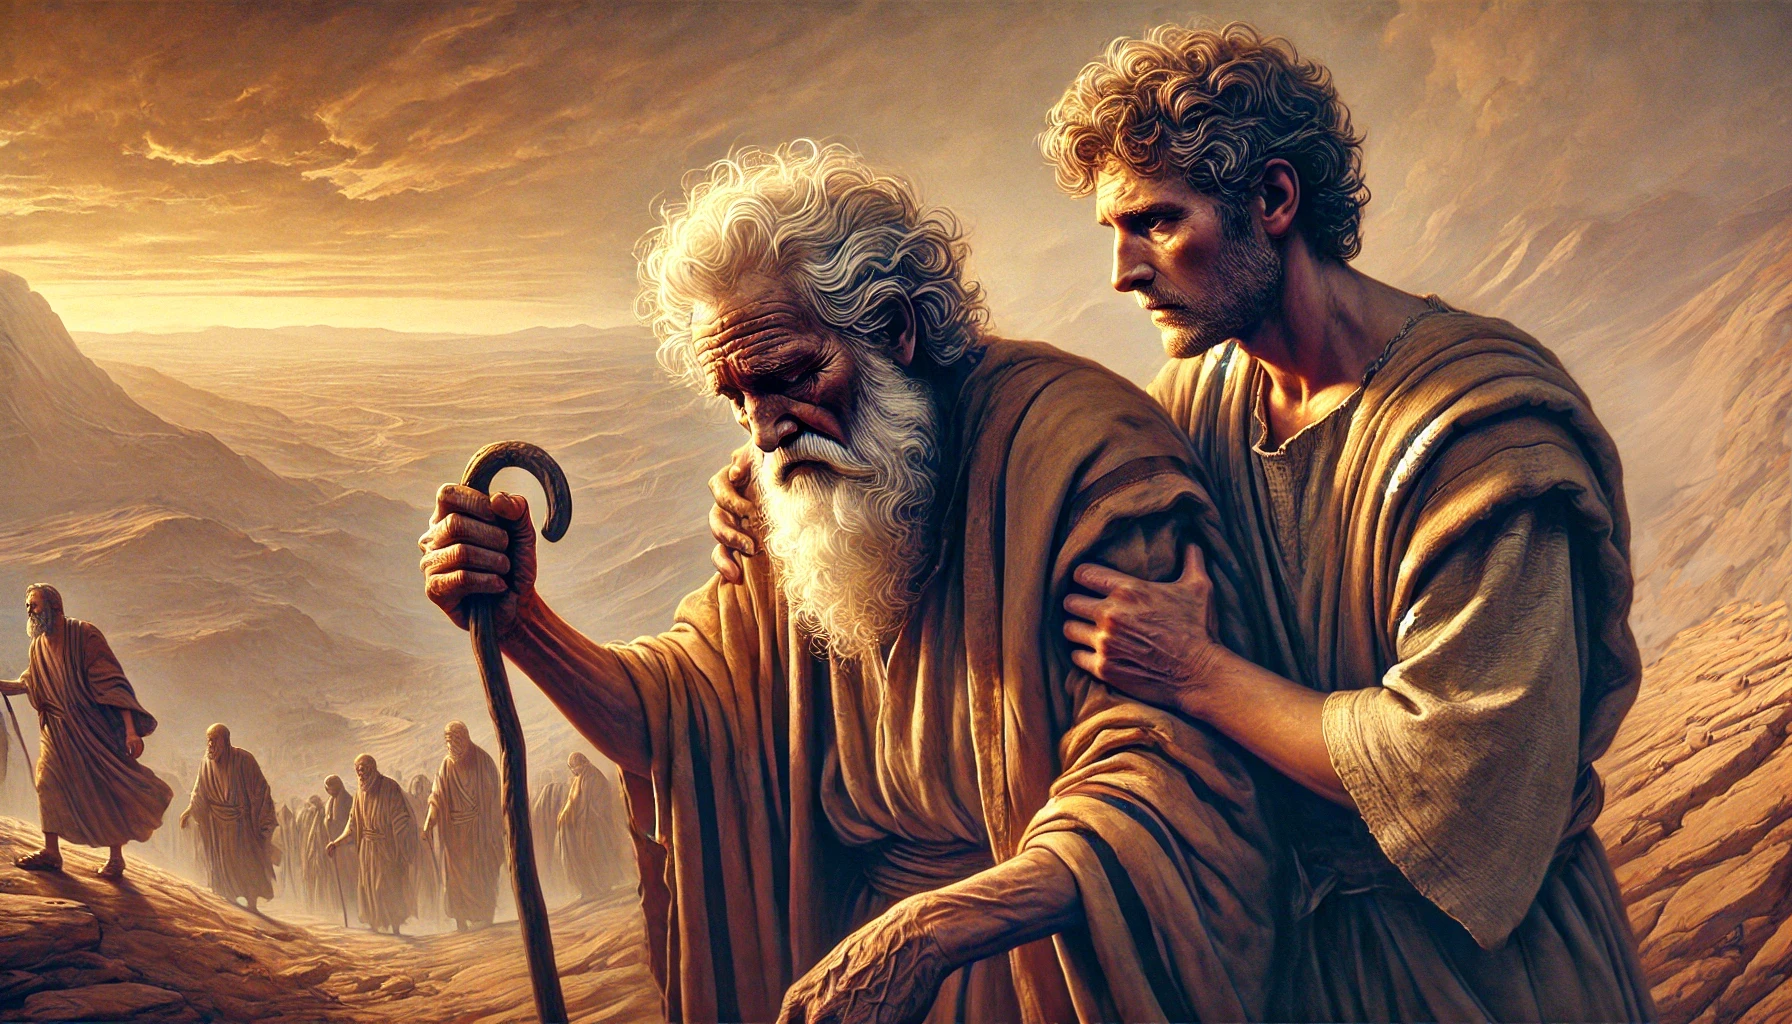
\includegraphics[width=0.7\linewidth]{graficas/deuteromonio}\\
	Moisés y Josué\\
\end{center}





\section*{Capítulo 1}


{Moisés recuerda a Israel las promesas de Jehová en Horeb } 



1:1 Estas son las palabras que habló Moisés a todo Israel a este lado del Jordán en el desierto, en el Arabá frente al Mar Rojo, entre Parán, Tofel, Labán, Hazerot y Dizahab.  
1:2 Once jornadas hay desde Horeb, camino del monte de Seir, hasta Cades-barnea.  
1:3 Y aconteció que a los cuarenta años, en el mes undécimo, el primero del mes, Moisés habló a los hijos de Israel conforme a todas las cosas que Jehová le había mandado acerca de ellos,  
1:4 después que derrotó a Sehón rey de los amorreos, el cual habitaba en Hesbón, y a Og rey de Basán que habitaba en Astarot en Edrei.  
1:5 De este lado del Jordán, en tierra de Moab, resolvió Moisés declarar esta ley, diciendo:  
1:6 Jehová nuestro Dios nos habló en Horeb, diciendo: Habéis estado bastante tiempo en este monte.  
1:7 Volveos e id al monte del amorreo y a todas sus comarcas, en el Arabá, en el monte, en los valles, en el Neguev, y junto a la costa del mar, a la tierra del cananeo, y al Líbano, hasta el gran río, el río Eufrates.  
1:8 Mirad, yo os he entregado la tierra; entrad y poseed la tierra que Jehová juró a vuestros padres Abraham, Isaac y Jacob, que les daría a ellos y a su descendencia después de ellos.  
Nombramiento de jueces   
1:9 En aquel tiempo yo os hablé diciendo: Yo solo no puedo llevaros.  
1:10 Jehová vuestro Dios os ha multiplicado, y he aquí hoy vosotros sois como las estrellas del cielo en multitud.  
1:11 ¡Jehová Dios de vuestros padres os haga mil veces más de lo que ahora sois, y os bendiga, como os ha prometido!  
1:12 ¿Cómo llevaré yo solo vuestras molestias, vuestras cargas y vuestros pleitos?  
1:13 Dadme de entre vosotros, de vuestras tribus, varones sabios y entendidos y expertos, para que yo los ponga por vuestros jefes.  
1:14 Y me respondisteis y dijisteis: Bueno es hacer lo que has dicho.  
1:15 Y tomé a los principales de vuestras tribus, varones sabios y expertos, y los puse por jefes sobre vosotros, jefes de millares, de centenas, de cincuenta y de diez, y gobernadores de vuestras tribus.  
1:16 Y entonces mandé a vuestros jueces, diciendo: Oíd entre vuestros hermanos, y juzgad justamente entre el hombre y su hermano, y el extranjero.  
1:17 No hagáis distinción de persona en el juicio; así al pequeño como al grande oiréis; no tendréis temor de ninguno, porque el juicio es de Dios; y la causa que os fuere difícil, la traeréis a mí, y yo la oiré.  
1:18 Os mandé, pues, en aquel tiempo, todo lo que habíais de hacer.  
Misión de los doce espías   
1:19 Y salidos de Horeb, anduvimos todo aquel grande y terrible desierto que habéis visto, por el camino del monte del amorreo, como Jehová nuestro Dios nos lo mandó; y llegamos hasta Cades- barnea.  
1:20 Entonces os dije: Habéis llegado al monte del amorreo, el cual Jehová nuestro Dios nos da.  
1:21 Mira, Jehová tu Dios te ha entregado la tierra; sube y toma posesión de ella, como Jehová el Dios de tus padres te ha dicho; no temas ni desmayes.  
1:22 Y vinisteis a mí todos vosotros, y dijisteis: Enviemos varones delante de nosotros que nos reconozcan la tierra, y a su regreso nos traigan razón del camino por donde hemos de subir, y de las ciudades adonde hemos de llegar.  
1:23 Y el dicho me pareció bien; y tomé doce varones de entre vosotros, un varón por cada tribu.  
1:24 Y se encaminaron, y subieron al monte, y llegaron hasta el valle de Escol, y reconocieron la tierra.  
1:25 Y tomaron en sus manos del fruto del país, y nos lo trajeron, y nos dieron cuenta, y dijeron: Es buena la tierra que Jehová nuestro Dios nos da.  
1:26 Sin embargo, no quisisteis subir, antes fuisteis rebeldes al mandato de Jehová vuestro Dios;  
1:27 y murmurasteis en vuestras tiendas, diciendo: Porque Jehová nos aborrece, nos ha sacado de tierra de Egipto, para entregarnos en manos del amorreo para destruirnos.  
1:28 ¿A dónde subiremos? Nuestros hermanos han atemorizado nuestro corazón, diciendo: Este pueblo es mayor y más alto que nosotros, las ciudades grandes y amuralladas hasta el cielo; y también vimos allí a los hijos de Anac. 
1:29 Entonces os dije: No temáis, ni tengáis miedo de ellos.  
1:30 Jehová vuestro Dios, el cual va delante de vosotros, él peleará por vosotros, conforme a todas las cosas que hizo por vosotros en Egipto delante de vuestros ojos.  
1:31 Y en el desierto has visto que Jehová tu Dios te ha traído, como trae el hombre a su hijo, por todo el camino que habéis andado, hasta llegar a este lugar.  
1:32 Y aun con esto no creísteis a Jehová vuestro Dios, 
1:33 quien iba delante de vosotros por el camino para reconoceros el lugar donde habíais de acampar, con fuego de noche para mostraros el camino por donde anduvieseis, y con nube de día.  
Dios castiga a Israel   
1:34 Y oyó Jehová la voz de vuestras palabras, y se enojó, y juró diciendo:  
1:35 No verá hombre alguno de estos, de esta mala generación, la buena tierra que juré que había de dar a vuestros padres,  
1:36 excepto Caleb hijo de Jefone; él la verá, y a él le daré la tierra que pisó, y a sus hijos; porque ha seguido fielmente a Jehová.  
1:37 También contra mí se airó Jehová por vosotros, y me dijo: Tampoco tú entrarás allá.  
1:38 Josué hijo de Nun, el cual te sirve, él entrará allá; anímale, porque él la hará heredar a Israel.  
1:39 Y vuestros niños, de los cuales dijisteis que servirían de botín, y vuestros hijos que no saben hoy lo bueno ni lo malo, ellos entrarán allá, y a ellos la daré, y ellos la heredarán.  
1:40 Pero vosotros volveos e id al desierto, camino del Mar Rojo.  
La derrota en Horma   
1:1:41 Entonces respondisteis y me dijisteis: Hemos pecado contra Jehová; nosotros subiremos y pelearemos, conforme a todo lo que Jehová nuestro Dios nos ha mandado. Y os armasteis cada uno con sus armas de guerra, y os preparasteis para subir al monte.  
1:42 Y Jehová me dijo: Diles: No subáis, ni peleéis, pues no estoy entre vosotros; para que no seáis derrotados por vuestros enemigos.  
1:43 Y os hablé, y no disteis oído; antes fuisteis rebeldes al mandato de Jehová, y persistiendo con altivez subisteis al monte.  
1:44 Pero salió a vuestro encuentro el amorreo, que habitaba en aquel monte, y os persiguieron como hacen las avispas, y os derrotaron en Seir, hasta Horma.  
1:45 Y volvisteis y llorasteis delante de Jehová, pero Jehová no escuchó vuestra voz, ni os prestó oído.  
1:46 Y estuvisteis en Cades por muchos días, los días que habéis estado allí.  
\section*{Capítulo 2}
Los años en el desierto  

2:1 Luego volvimos y salimos al desierto, camino del Mar Rojo, como Jehová me había dicho; y rodeamos el monte de Seir por mucho tiempo.  
2:2 Y Jehová me habló, diciendo:  
2:3 Bastante habéis rodeado este monte; volveos al norte.  
2:4 Y manda al pueblo, diciendo: Pasando vosotros por el territorio de vuestros hermanos los hijos de Esaú, que habitan en Seir, ellos tendrán miedo de vosotros; mas vosotros guardaos mucho.  
2:5 No os metáis con ellos, porque no os daré de su tierra ni aun lo que cubre la planta de un pie; porque yo he dado por heredad a Esaú el monte de Seir.  
2:6 Compraréis de ellos por dinero los alimentos, y comeréis; y también compraréis de ellos el agua, y beberéis;  
2:7 pues Jehová tu Dios te ha bendecido en toda obra de tus manos; él sabe que andas por este gran desierto; estos cuarenta años Jehová tu Dios ha estado contigo, y nada te ha faltado.  
2:8 Y nos alejamos del territorio de nuestros hermanos los hijos de Esaú, que habitaban en Seir, por el camino del Arabá desde Elat y Ezión-geber; y volvimos, y tomamos el camino del desierto de Moab.  
2:9 Y Jehová me dijo: No molestes a Moab, ni te empeñes con ellos en guerra, porque no te daré posesión de su tierra; porque yo he dado a Ar por heredad a los hijos de Lot.  
2:10 (Los emitas habitaron en ella antes, pueblo grande y numeroso, y alto como los hijos de Anac.  
2:11 Por gigantes eran ellos tenidos también, como los hijos de Anac; y los moabitas los llaman emitas.  
2:12 Y en Seir habitaron antes los horeos, a los cuales echaron los hijos de Esaú; y los arrojaron de su presencia, y habitaron en lugar de ellos, como hizo Israel en la tierra que les dio Jehová por posesión.)  
2:13 Levantaos ahora, y pasad el arroyo de Zered. Y pasamos el arroyo de Zered.  
2:14 Y los días que anduvimos de Cades-barnea hasta cuando pasamos el arroyo de Zered fueron treinta y ocho años; hasta que se acabó toda la generación de los hombres de guerra de en medio del campamento, como Jehová les había jurado. 
2:15 Y también la mano de Jehová vino sobre ellos para destruirlos de en medio del campamento, hasta acabarlos.  
2:16 Y aconteció que después que murieron todos los hombres de guerra de entre el pueblo,  
2:17 Jehová me habló, diciendo:  
2:18 Tú pasarás hoy el territorio de Moab, a Ar.  
2:19 Y cuando te acerques a los hijos de Amón, no los molestes, ni contiendas con ellos; porque no te daré posesión de la tierra de los hijos de Amón, pues a los hijos de Lot la he dado por heredad.  
2:20 (Por tierra de gigantes fue también ella tenida; habitaron en ella gigantes en otro tiempo, a los cuales los amonitas llamaban zomzomeos;  
2:21 pueblo grande y numeroso, y alto, como los hijos de Anac; a los cuales Jehová destruyó delante de los amonitas. Estos sucedieron a aquéllos, y habitaron en su lugar,  
2:22 como hizo Jehová con los hijos de Esaú que habitaban en Seir, delante de los cuales destruyó a los horeos; y ellos sucedieron a éstos, y habitaron en su lugar hasta hoy.  
2:23 Y a los aveos que habitaban en aldeas hasta Gaza, los caftoreos que salieron de Caftor los destruyeron, y habitaron en su lugar.)  
2:24 Levantaos, salid, y pasad el arroyo de Arnón; he aquí he entregado en tu mano a Sehón rey de Hesbón, amorreo, y a su tierra; comienza a tomar posesión de ella, y entra en guerra con él.  
2:25 Hoy comenzaré a poner tu temor y tu espanto sobre los pueblos debajo de todo el cielo, los cuales oirán tu fama, y temblarán y se angustiarán delante de ti.  
Israel derrota a Sehón   
2:26 Y envié mensajeros desde el desierto de Cademot a Sehón rey de Hesbón con palabras de paz, diciendo:  
2:27 Pasaré por tu tierra por el camino; por el camino iré, sin apartarme ni a diestra ni a siniestra.  
2:28 La comida me venderás por dinero, y comeré; el agua también me darás por dinero, y beberé; solamente pasaré a pie,  
2:29 como lo hicieron conmigo los hijos de Esaú que habitaban en Seir, y los moabitas que habitaban en Ar; hasta que cruce el Jordán a la tierra que nos da Jehová nuestro Dios.  
2:30 Mas Sehón rey de Hesbón no quiso que pasásemos por el territorio suyo; porque Jehová tu Dios había endurecido su espíritu, y obstinado su corazón para entregarlo en tu mano, como hasta hoy.  
2:31 Y me dijo Jehová: He aquí yo he comenzado a entregar delante de ti a Sehón y a su tierra; comienza a tomar posesión de ella para que la heredes.  
2:32 Y nos salió Sehón al encuentro, él y todo su pueblo, para pelear en Jahaza.  
2:33 Mas Jehová nuestro Dios lo entregó delante de nosotros; y lo derrotamos a él y a sus hijos, y a todo su pueblo.  
2:34 Tomamos entonces todas sus ciudades, y destruimos todas las ciudades, hombres, mujeres y niños; no dejamos ninguno.  
2:35 Solamente tomamos para nosotros los ganados, y los despojos de las ciudades que habíamos tomado.  
2:36 Desde Aroer, que está junto a la ribera del arroyo de Arnón, y la ciudad que está en el valle, hasta Galaad, no hubo ciudad que escapase de nosotros; todas las entregó Jehová nuestro Dios en nuestro poder.  
2:37 Solamente a la tierra de los hijos de Amón no llegamos; ni a todo lo que está a la orilla del arroyo de Jaboc ni a las ciudades del monte, ni a lugar alguno que Jehová nuestro Dios había prohibido.  
\section*{Capítulo 3}
Israel derrota a Og rey de Basán  

3:1 Volvimos, pues, y subimos camino de Basán, y nos salió al encuentro Og rey de Basán para pelear, él y todo su pueblo, en Edrei.  
3:2 Y me dijo Jehová: No tengas temor de él, porque en tu mano he entregdo a él y a todo su pueblo, con su tierra; y harás con él como hiciste con Sehón rey amorreo, que habitaba en Hesbón.  
3:3 Y Jehová nuestro Dios entregó también en nuestra mano a Og rey de Basán, y a todo su pueblo, al cual derrotamos hasta acabar con todos.  
3:4 Y tomamos entonces todas sus ciudades; no quedó ciudad que no les tomásemos; sesenta ciudades, toda la tierra de Argob, del reino de Og en Basán.  
3:5 Todas estas eran ciudades fortificadas con muros altos, con puertas y barras, sin contar otras muchas ciudades sin muro.  
3:6 Y las destruimos, como hicimos a Sehón rey de Hesbón, matando en toda ciudad a hombres, mujeres y niños.  
3:7 Y tomamos para nosotros todo el ganado, y los despojos de las ciudades.  
3:8 También tomamos en aquel tiempo la tierra desde el arroyo de Arnón hasta el monte de Hermón, de manos de los dos reyes amorreos que estaban a este lado del Jordán.  
3:9 (Los sidonios llaman a Hermón, Sirión; y los amorreos, Senir.)  
3:10 Todas las ciudades de la llanura, y todo Galaad, y todo Basán hasta Salca y Edrei, ciudades del reino de Og en Basán.  
3:11 Porque únicamente Og rey de Basán había quedado del resto de los gigantes. Su cama, una cama de hierro, ¿no está en Rabá de los hijos de Amón? La longitud de ella es de nueve codos, y su anchura de cuatro codos, según el codo de un hombre.  
Rubén, Gad y la media tribu de Manasés se establecen al oriente del Jordán  

3:12 Y esta tierra que heredamos en aquel tiempo, desde Aroer, que está junto al arroyo de Arnón, y la mitad del monte de Galaad con sus ciudades, la di a los rubenitas y a los gaditas;  
3:13 y el resto de Galaad, y todo Basán, del reino de Og, toda la tierra de Argob, que se llamaba la tierra de los gigantes, lo di a la media tribu de Manasés.  
3:14 Jair hijo de Manasés tomó toda la tierra de Argob hasta el límite con Gesur y Maaca, y la llamó por su nombre, Basán- havot-jair, hasta hoy.  
3:15 Y Galaad se lo di a Maquir.  
3:16 Y a los rubenitas y gaditas les di de Galaad hasta el arroyo de Arnón, teniendo por límite el medio del valle, hasta el arroyo de Jaboc, el cual es límite de los hijos de Amón;  
3:17 también el Arabá, con el Jordán como límite desde Cineret hasta el mar del Arabá, el Mar Salado, al pie de las laderas del Pisga al oriente.  
3:18 Y os mandé entonces, diciendo: Jehová vuestro Dios os ha dado esta tierra por heredad; pero iréis armados todos los valientes delante de vuestros hermanos los hijos de Israel.  
3:19 Solamente vuestras mujeres, vuestros hijos y vuestros ganados (yo sé que tenéis mucho ganado), quedarán en las ciudades que os he dado,  
3:20 hasta que Jehová dé reposo a vuestros hermanos, así como a vosotros, y hereden ellos también la tierra que Jehová vuestro Dios les da al otro lado del Jordán; entonces os volveréis cada uno a la heredad que yo os he dado.  
3:21 Ordené también a Josué en aquel tiempo, diciendo: Tus ojos vieron todo lo que Jehová vuestro Dios ha hecho a aquellos dos reyes; así hará Jehová a todos los reinos a los cuales pasarás tú.  
3:22 No los temáis; porque Jehová vuestro Dios, él es el que pelea por vosotros.  
No se le permite a Moisés entrar a Canaán  
3:23 Y oré a Jehová en aquel tiempo, diciendo:  
3:24 Señor Jehová, tú has comenzado a mostrar a tu siervo tu grandeza, y tu mano poderosa; porque ¿qué dios hay en el cielo ni en la tierra que haga obras y proezas como las tuyas?  
3:25 Pase yo, te ruego, y vea aquella tierra buena que está más allá del Jordán, aquel buen monte, y el Líbano.  
3:26 Pero Jehová se había enojado contra mí a causa de vosotros, por lo cual no me escuchó; y me dijo Jehová: Basta, no me hables más de este asunto.  
3:27 Sube a la cumbre del Pisga y alza tus ojos al oeste, y al norte, y al sur, y al este, y mira con tus propios ojos; porque no pasarás el Jordán.  
3:28 Y manda a Josué, y anímalo, y fortalécelo; porque él ha de pasar delante de este pueblo, y él les hará heredar la tierra que verás.  
3:29 Y paramos en el valle delante de Bet-peor.  
\section*{Capítulo 4 }
Moisés exhorta a la obediencia  

4:1 Ahora, pues, oh Israel, oye los estatutos y decretos que yo os enseño, para que los ejecutéis, y viváis, y entréis y poseáis la tierra que Jehová el Dios de vuestros padres os da.  
4:2 No añadiréis a la palabra que yo os mando, ni disminuiréis de ella, para que guardéis los mandamientos de Jehová vuestro Dios que yo os ordene.  
4:3 Vuestros ojos vieron lo que hizo Jehová con motivo de Baal- peor; que a todo hombre que fue en pos de Baal-peor destruyó Jehová tu Dios de en medio de ti.  
4:4 Mas vosotros que seguisteis a Jehová vuestro Dios, todos estáis vivos hoy.  
4:5 Mirad, yo os he enseñado estatutos y decretos, como Jehová mi Dios me mandó, para que hagáis así en medio de la tierra en la cual entráis para tomar posesión de ella.  
4:6 Guardadlos, pues, y ponedlos por obra; porque esta es vuestra sabiduría y vuestra inteligencia ante los ojos de los pueblos, los cuales oirán todos estos estatutos, y dirán: Ciertamente pueblo sabio y entendido, nación grande es esta.  
4:7 Porque ¿qué nación grande hay que tenga dioses tan cercanos a ellos como lo está Jehová nuestro Dios en todo cuanto le pedimos?  
4:8 Y ¿qué nación grande hay que tenga estatutos y juicios justos como es toda esta ley que yo pongo hoy delante de vosotros?  
La experiencia de Israel en Horeb  
4:9 Por tanto, guárdate, y guarda tu alma con diligencia, para que no te olvides de las cosas que tus ojos han visto, ni se aparten de tu corazón todos los días de tu vida; antes bien, las enseñarás a tus hijos, y a los hijos de tus hijos.  
4:10 El día que estuviste delante de Jehová tu Dios en Horeb, cuando Jehová me dijo: Reúneme el pueblo, para que yo les haga oír mis palabras, las cuales aprenderán, para temerme todos los días que vivieren sobre la tierra, y las enseñarán a sus hijos;  
4:11 y os acercasteis y os pusisteis al pie del monte; y el monte ardía en fuego hasta en medio de los cielos con tinieblas, nube y oscuridad;  
4:12 y habló Jehová con vosotros de en medio del fuego; oísteis la voz de sus palabras, mas a excepción de oír la voz, ninguna figura visteis.  
4:13 Y él os anunció su pacto, el cual os mandó poner por obra; los diez mandamientos, y los escribió en dos tablas de piedra. 
4:14 A mí también me mandó Jehová en aquel tiempo que os enseñase los estatutos y juicios, para que los pusieseis por obra en la tierra a la cual pasáis a tomar posesión de ella.  
Advertencia contra la idolatría  
4:15 Guardad, pues, mucho vuestras almas; pues ninguna figura visteis el día que Jehová habló con vosotros de en medio del fuego;  
4:16 para que no os corrompáis y hagáis para vosotros escultura, imagen de figura alguna, efigie de varón o hembra,  
4:17 figura de animal alguno que está en la tierra, figura de ave alguna alada que vuele por el aire,  
4:18 figura de ningún animal que se arrastre sobre la tierra, figura de pez alguno que haya en el agua debajo de la tierra.  
4:19 No sea que alces tus ojos al cielo, y viendo el sol y la luna y las estrellas, y todo el ejército del cielo, seas impulsado, y te inclines a ellos y les sirvas; porque Jehová tu Dios los ha concedido a todos los pueblos debajo de todos los cielos.  
4:20 Pero a vosotros Jehová os tomó, y os ha sacado del horno de hierro, de Egipto, para que seáis el pueblo de su heredad como en este día.  
4:21 Y Jehová se enojó contra mí por causa de vosotros, y juró que yo no pasaría el Jordán, ni entraría en la buena tierra que Jehová tu Dios te da por heredad.  
4:22 Así que yo voy a morir en esta tierra, y no pasaré el Jordán; mas vosotros pasaréis, y poseeréis aquella buena tierra.  
4:23 Guardaos, no os olvidéis del pacto de Jehová vuestro Dios, que él estableció con vosotros, y no os hagáis escultura o imagen de ninguna cosa que Jehová tu Dios te ha prohibido.  
4:24 Porque Jehová tu Dios es fuego consumidor, Dios celoso.  
4:25 Cuando hayáis engendrado hijos y nietos, y hayáis envejecido en la tierra, si os corrompiereis e hiciereis escultura o imagen de cualquier cosa, e hiciereis lo malo ante los ojos de Jehová vuestro Dios, para enojarlo;  
4:26 yo pongo hoy por testigos al cielo y a la tierra, que pronto pereceréis totalmente de la tierra hacia la cual pasáis el Jordán para tomar posesión de ella; no estaréis en ella largos días sin que seáis destruidos.  
4:27 Y Jehová os esparcirá entre los pueblos, y quedaréis pocos en número entre las naciones a las cuales os llevará Jehová.  
4:28 Y serviréis allí a dioses hechos de manos de hombres, de madera y piedra, que no ven, ni oyen, ni comen, ni huelen.  
4:29 Mas si desde allí buscares a Jehová tu Dios, lo hallarás, si lo buscares de todo tu corazón y de toda tu alma.  
4:30 Cuando estuvieres en angustia, y te alcanzaren todas estas cosas, si en los postreros días te volvieres a Jehová tu Dios, y oyeres su voz;  
4:31 porque Dios misericordioso es Jehová tu Dios; no te dejará, ni te destruirá, ni se olvidará del pacto que les juró a tus padres.  
4:32 Porque pregunta ahora si en los tiempos pasados que han sido antes de ti, desde el día que creó Dios al hombre sobre la tierra, si desde un extremo del cielo al otro se ha hecho cosa semejante a esta gran cosa, o se haya oído otra como ella.  
4:33 ¿Ha oído pueblo alguno la voz de Dios, hablando de en medio del fuego, como tú la has oído, sin perecer?  
4:34 ¿O ha intentado Dios venir a tomar para sí una nación de en medio de otra nación, con pruebas, con señales, con milagros y con guerra, y mano poderosa y brazo extendido, y hechos aterradores como todo lo que hizo con vosotros Jehová vuestro Dios en Egipto ante tus ojos?  
4:35 A ti te fue mostrado, para que supieses que Jehová es Dios, y no hay otro fuera de él.  
4:36 Desde los cielos te hizo oír su voz, para enseñarte; y sobre la tierra te mostró su gran fuego, y has oído sus palabras de en medio del fuego.  
4:37 Y por cuanto él amó a tus padres, escogió a su descendencia después de ellos, y te sacó de Egipto con su presencia y con su gran poder,  
4:38 para echar de delante de tu presencia naciones grandes y más fuertes que tú, y para introducirte y darte su tierra por heredad, como hoy.  
4:39 Aprende pues, hoy, y reflexiona en tu corazón que Jehová es Dios arriba en el cielo y abajo en la tierra, y no hay otro.  
4:40 Y guarda sus estatutos y sus mandamientos, los cuales yo te mando hoy, para que te vaya bien a ti y a tus hijos después de ti, y prolongues tus días sobre la tierra que Jehová tu Dios te da para siempre.  
Las ciudades de refugio al oriente del Jordán  
4:41 Entonces apartó Moisés tres ciudades a este lado del Jordán al nacimiento del sol,  
4:42 para que huyese allí el homicida que matase a su prójimo sin intención, sin haber tenido enemistad con él nunca antes; y que huyendo a una de estas ciudades salvase su vida:  
4:43 Beser en el desierto, en tierra de la llanura, para los rubenitas; Ramot en Galaad para los gaditas, y Golán en Basán para los de Manasés.  
Moisés recapitula la promulgación de la ley  
4:44 Esta, pues, es la ley que Moisés puso delante de los hijos de Israel.  
4:45 Estos son los testimonios, los estatutos y los decretos que habló Moisés a los hijos de Israel cuando salieron de Egipto;  
4:46 a este lado del Jordán, en el valle delante de Bet-peor, en la tierra de Sehón rey de los amorreos que habitaba en Hesbón, al cual derrotó Moisés con los hijos de Israel, cuando salieron de Egipto;  
4:47 y poseyeron su tierra, y la tierra de Og rey de Basán; dos reyes de los amorreos que estaban de este lado del Jordán, al oriente. 
4:48 Desde Aroer, que está junto a la ribera del arroyo de Arnón, hasta el monte de Sion, que es Hermón; 
4:49 y todo el Arabá de este lado del Jordán, al oriente, hasta el mar del Arabá, al pie de las laderas del Pisga.  
\section*{Capítulo 5 }
Los Diez Mandamientos   

5:1 Llamó Moisés a todo Israel y les dijo: Oye, Israel, los estatutos y decretos que yo pronuncio hoy en vuestros oídos; aprendedlos, y guardadlos, para ponerlos por obra.  
5:2 Jehová nuestro Dios hizo pacto con nosotros en Horeb.  
5:3 No con nuestros padres hizo Jehová este pacto, sino con nosotros todos los que estamos aquí hoy vivos.  
5:4 Cara a cara habló Jehová con vosotros en el monte de en medio del fuego.  
5:5 Yo estaba entonces entre Jehová y vosotros, para declararos la palabra de Jehová; porque vosotros tuvisteis temor del fuego, y no subisteis al monte. Dijo:  
5:6 Yo soy Jehová tu Dios, que te saqué de tierra de Egipto, de casa de servidumbre.  
5:7 No tendrás dioses ajenos delante de mí.  
5:8 No harás para ti escultura, ni imagen alguna de cosa que está arriba en los cielos, ni abajo en la tierra, ni en las aguas debajo de la tierra.  
5:9 No te inclinarás a ellas ni las servirás; porque yo soy Jehová tu Dios, fuerte, celoso, que visito la maldad de los padres sobre los hijos hasta la tercera y cuarta generación de los que me aborrecen,  
5:10 y que hago misericordia a millares, a los que me aman y guardan mis mandamientos.  
5:11 No tomarás el nombre de Jehová tu Dios en vano; porque Jehová no dará por inocente al que tome su nombre en vano.  
5:12 Guardarás el día de reposo para santificarlo, como Jehová tu Dios te ha mandado. 
5:13 Seis días trabajarás, y harás toda tu obra;  
5:14 mas el séptimo día es reposo a Jehová tu Dios; ninguna obra harás tú, ni tu hijo, ni tu hija, ni tu siervo, ni tu sierva, ni tu buey, ni tu asno, ni ningún animal tuyo, ni el extranjero que está dentro de tus puertas, para que descanse tu siervo y tu sierva como tú.  
5:15 Acuérdate que fuiste siervo en tierra de Egipto, y que Jehová tu Dios te sacó de allá con mano fuerte y brazo extendido; por lo cual Jehová tu Dios te ha mandado que guardes el día de reposo.  
5:16 Honra a tu padre y a tu madre, como Jehová tu Dios te ha mandado, para que sean prolongados tus días, y para que te vaya bien sobre la tierra que Jehová tu Dios te da.  
5:17 No matarás. 
5:18 No cometerás adulterio.  
5:19 No hurtarás. 
5:20 No dirás falso testimonio contra tu prójimo.  
5:21 No codiciarás la mujer de tu prójimo, ni desearás la casa de tu prójimo, ni su tierra, ni su siervo, ni su sierva, ni su buey, ni su asno, ni cosa alguna de tu prójimo.  
El terror del pueblo   
5:22 Estas palabras habló Jehová a toda vuestra congregación en el monte, de en medio del fuego, de la nube y de la oscuridad, a gran voz; y no añadió más. Y las escribió en dos tablas de piedra, las cuales me dio a mí.  
5:23 Y aconteció que cuando vosotros oísteis la voz de en medio de las tinieblas, y visteis al monte que ardía en fuego, vinisteis a mí, todos los príncipes de vuestras tribus, y vuestros ancianos,  
5:24 y dijisteis: He aquí Jehová nuestro Dios nos ha mostrado su gloria y su grandeza, y hemos oído su voz de en medio del fuego; hoy hemos visto que Jehová habla al hombre, y éste aún vive.  
5:25 Ahora, pues, ¿por qué vamos a morir? Porque este gran fuego nos consumirá; si oyéremos otra vez la voz de Jehová nuestro Dios, moriremos.  
5:26 Porque ¿qué es el hombre, para que oiga la voz del Dios viviente que habla de en medio del fuego, como nosotros la oímos, y aún viva?  
5:27 Acércate tú, y oye todas las cosas que dijere Jehová nuestro Dios; y tú nos dirás todo lo que Jehová nuestro Dios te dijere, y nosotros oiremos y haremos.  
5:28 Y oyó Jehová la voz de vuestras palabras cuando me hablabais, y me dijo Jehová: He oído la voz de las palabras de este pueblo, que ellos te han hablado; bien está todo lo que han dicho.  
5:29 ¡Quién diera que tuviesen tal corazón, que me temiesen y guardasen todos los días todos mis mandamientos, para que a ellos y a sus hijos les fuese bien para siempre!  
5:30 Ve y diles: Volveos a vuestras tiendas.  
5:31 Y tú quédate aquí conmigo, y te diré todos los mandamientos y estatutos y decretos que les enseñarás, a fin de que los pongan ahora por obra en la tierra que yo les doy por posesión.  
5:32 Mirad, pues, que hagáis como Jehová vuestro Dios os ha mandado; no os apartéis a diestra ni a siniestra.  
5:33 Andad en todo el camino que Jehová vuestro Dios os ha mandado, para que viváis y os vaya bien, y tengáis largos días en la tierra que habéis de poseer.  
\section*{Capítulo 6 }
El gran mandamiento  

6:1 Estos, pues, son los mandamientos, estatutos y decretos que Jehová vuestro Dios mandó que os enseñase, para que los pongáis por obra en la tierra a la cual pasáis vosotros para tomarla;  
6:2 para que temas a Jehová tu Dios, guardando todos sus estatutos y sus mandamientos que yo te mando, tú, tu hijo, y el hijo de tu hijo, todos los días de tu vida, para que tus días sean prolongados.  
6:3 Oye, pues, oh Israel, y cuida de ponerlos por obra, para que te vaya bien en la tierra que fluye leche y miel, y os multipliquéis, como te ha dicho Jehová el Dios de tus padres.  
6:4 Oye, Israel: Jehová nuestro Dios, Jehová uno es.  
6:5 Y amarás a Jehová tu Dios de todo tu corazón, y de toda tu alma, y con todas tus fuerzas.  
6:6 Y estas palabras que yo te mando hoy, estarán sobre tu corazón;  
6:7 y las repetirás a tus hijos, y hablarás de ellas estando en tu casa, y andando por el camino, y al acostarte, y cuando te levantes.  
6:8 Y las atarás como una señal en tu mano, y estarán como frontales entre tus ojos;  
6:9 y las escribirás en los postes de tu casa, y en tus puertas.  
Exhortaciones a la obediencia  
6:10 Cuando Jehová tu Dios te haya introducido en la tierra que juró a tus padres Abraham, Isaac y Jacob que te daría, en ciudades grandes y buenas que tú no edificaste,  
6:11 y casas llenas de todo bien, que tú no llenaste, y cisternas cavadas que tú no cavaste, viñas y olivares que no plantaste, y luego que comas y te sacies,  
6:12 cuídate de no olvidarte de Jehová, que te sacó de la tierra de Egipto, de casa de servidumbre.  
6:13 A Jehová tu Dios temerás, y a él solo servirás, y por su nombre jurarás.  
6:14 No andaréis en pos de dioses ajenos, de los dioses de los pueblos que están en vuestros contornos;  
6:15 porque el Dios celoso, Jehová tu Dios, en medio de ti está; para que no se inflame el furor de Jehová tu Dios contra ti, y te destruya de sobre la tierra.  
6:16 No tentaréis a Jehová vuestro Dios, como lo tentasteis en Masah.  
6:17 Guardad cuidadosamente los mandamientos de Jehová vuestro Dios, y sus testimonios y sus estatutos que te ha mandado.  
6:18 Y haz lo recto y bueno ante los ojos de Jehová, para que te vaya bien, y entres y poseas la buena tierra que Jehová juró a tus padres;  
6:19 para que él arroje a tus enemigos de delante de ti, como Jehová ha dicho.  
6:20 Mañana cuando te preguntare tu hijo, diciendo: ¿Qué significan los testimonios y estatutos y decretos que Jehová nuestro Dios os mandó?  
6:21 entonces dirás a tu hijo: Nosotros éramos siervos de Faraón en Egipto, y Jehová nos sacó de Egipto con mano poderosa.  
6:22 Jehová hizo señales y milagros grandes y terribles en Egipto, sobre Faraón y sobre toda su casa, delante de nuestros ojos;  
6:23 y nos sacó de allá, para traernos y darnos la tierra que juró a nuestros padres.  
6:24 Y nos mandó Jehová que cumplamos todos estos estatutos, y que temamos a Jehová nuestro Dios, para que nos vaya bien todos los días, y para que nos conserve la vida, como hasta hoy.  
6:25 Y tendremos justicia cuando cuidemos de poner por obra todos estos mandamientos delante de Jehová nuestro Dios, como él nos ha mandado.  
\section*{Capítulo 7 }
Advertencias contra la idolatría de Canaán   

7:1 Cuando Jehová tu Dios te haya introducido en la tierra en la cual entrarás para tomarla, y haya echado de delante de ti a muchas naciones, al heteo, al gergeseo, al amorreo, al cananeo, al ferezeo, al heveo y al jebuseo, siete naciones mayores y más poderosas que tú,  
7:2 y Jehová tu Dios las haya entregado delante de ti, y las hayas derrotado, las destruirás del todo; no harás con ellas alianza, ni tendrás de ellas misericordia.  
7:3 Y no emparentarás con ellas; no darás tu hija a su hijo, ni tomarás a su hija para tu hijo.  
7:4 Porque desviará a tu hijo de en pos de mí, y servirán a dioses ajenos; y el furor de Jehová se encenderá sobre vosotros, y te destruirá pronto.  
7:5 Mas así habéis de hacer con ellos: sus altares destruiréis, y quebraréis sus estatuas, y destruiréis sus imágenes de Asera, y quemaréis sus esculturas en el fuego.  
Un pueblo santo para Jehová  
7:6 Porque tú eres pueblo santo para Jehová tu Dios; Jehová tu Dios te ha escogido para serle un pueblo especial, más que todos los pueblos que están sobre la tierra.  
7:7 No por ser vosotros más que todos los pueblos os ha querido Jehová y os ha escogido, pues vosotros erais el más insignificante de todos los pueblos;  
7:8 sino por cuanto Jehová os amó, y quiso guardar el juramento que juró a vuestros padres, os ha sacado Jehová con mano poderosa, y os ha rescatado de servidumbre, de la mano de Faraón rey de Egipto.  
7:9 Conoce, pues, que Jehová tu Dios es Dios, Dios fiel, que guarda el pacto y la misericordia a los que le aman y guardan sus mandamientos, hasta mil generaciones;  
7:10 y que da el pago en persona al que le aborrece, destruyéndolo; y no se demora con el que le odia, en persona le dará el pago.  
7:11 Guarda, por tanto, los mandamientos, estatutos y decretos que yo te mando hoy que cumplas.  
Bendiciones de la obediencia   
7:12 Y por haber oído estos decretos y haberlos guardado y puesto por obra, Jehová tu Dios guardará contigo el pacto y la misericordia que juró a tus padres.  
7:13 Y te amará, te bendecirá y te multiplicará, y bendecirá el fruto de tu vientre y el fruto de tu tierra, tu grano, tu mosto, tu aceite, la cría de tus vacas, y los rebaños de tus ovejas, en la tierra que juró a tus padres que te daría.  
7:14 Bendito serás más que todos los pueblos; no habrá en ti varón ni hembra estéril, ni en tus ganados.  
7:15 Y quitará Jehová de ti toda enfermedad; y todas las malas plagas de Egipto, que tú conoces, no las pondrá sobre ti, antes las pondrá sobre todos los que te aborrecieren.  
7:16 Y consumirás a todos los pueblos que te da Jehová tu Dios; no los perdonará tu ojo, ni servirás a sus dioses, porque te será tropiezo.  
7:17 Si dijeres en tu corazón: Estas naciones son mucho más numerosas que yo; ¿cómo las podré exterminar?  
7:18 no tengas temor de ellas; acuérdate bien de lo que hizo Jehová tu Dios con Faraón y con todo Egipto;  
7:19 de las grandes pruebas que vieron tus ojos, y de las señales y milagros, y de la mano poderosa y el brazo extendido con que Jehová tu Dios te sacó; así hará Jehová tu Dios con todos los pueblos de cuya presencia tú temieres.  
7:20 También enviará Jehová tu Dios avispas sobre ellos, hasta que perezcan los que quedaren y los que se hubieren escondido de delante de ti.  
7:21 No desmayes delante de ellos, porque Jehová tu Dios está en medio de ti, Dios grande y temible.  
7:22 Y Jehová tu Dios echará a estas naciones de delante de ti poco a poco; no podrás acabar con ellas en seguida, para que las fieras del campo no se aumenten contra ti.  
7:23 Mas Jehová tu Dios las entregará delante de ti, y él las quebrantará con grande destrozo, hasta que sean destruidas.  
7:24 El entregará sus reyes en tu mano, y tú destruirás el nombre de ellos de debajo del cielo; nadie te hará frente hasta que los destruyas.  
7:25 Las esculturas de sus dioses quemarás en el fuego; no codiciarás plata ni oro de ellas para tomarlo para ti, para que no tropieces en ello, pues es abominación a Jehová tu Dios;  
7:26 y no traerás cosa abominable a tu casa, para que no seas anatema; del todo la aborrecerás y la abominarás, porque es anatema.  
\section*{Capítulo 8 }
La buena tierra que han de poseer  

8:1 Cuidaréis de poner por obra todo mandamiento que yo os ordeno hoy, para que viváis, y seáis multiplicados, y entréis y poseáis la tierra que Jehová prometió con juramento a vuestros padres.  
8:2 Y te acordarás de todo el camino por donde te ha traído Jehová tu Dios estos cuarenta años en el desierto, para afligirte, para probarte, para saber lo que había en tu corazón, si habías de guardar o no sus mandamientos.  
8:3 Y te afligió, y te hizo tener hambre, y te sustentó con maná, comida que no conocías tú, ni tus padres la habían conocido, para hacerte saber que no sólo de pan vivirá el hombre, mas de todo lo que sale de la boca de Jehová vivirá el hombre.  
8:4 Tu vestido nunca se envejeció sobre ti, ni el pie se te ha hinchado en estos cuarenta años.  
8:5 Reconoce asimismo en tu corazón, que como castiga el hombre a su hijo, así Jehová tu Dios te castiga.  
8:6 Guardarás, pues, los mandamientos de Jehová tu Dios, andando en sus caminos, y temiéndole.  
8:7 Porque Jehová tu Dios te introduce en la buena tierra, tierra de arroyos, de aguas, de fuentes y de manantiales, que brotan en vegas y montes;  
8:8 tierra de trigo y cebada, de vides, higueras y granados; tierra de olivos, de aceite y de miel;  
8:9 tierra en la cual no comerás el pan con escasez, ni te faltará nada en ella; tierra cuyas piedras son hierro, y de cuyos montes sacarás cobre.  
8:10 Y comerás y te saciarás, y bendecirás a Jehová tu Dios por la buena tierra que te habrá dado.  
Amonestación de no olvidar a Dios  
8:11 Cuídate de no olvidarte de Jehová tu Dios, para cumplir sus mandamientos, sus decretos y sus estatutos que yo te ordeno hoy;  
8:12 no suceda que comas y te sacies, y edifiques buenas casas en que habites,  
8:13 y tus vacas y tus ovejas se aumenten, y la plata y el oro se te multipliquen, y todo lo que tuvieres se aumente;  
8:14 y se enorgullezca tu corazón, y te olvides de Jehová tu Dios, que te sacó de tierra de Egipto, de casa de servidumbre;  
8:15 que te hizo caminar por un desierto grande y espantoso, lleno de serpientes ardientes, y de escorpiones, y de sed, donde no había agua, y él te sacó agua de la roca del pedernal;  
8:16 que te sustentó con maná en el desierto, comida que tus padres no habían conocido, afligiéndote y probándote, para a la postre hacerte bien;  
8:17 y digas en tu corazón: Mi poder y la fuerza de mi mano me han traído esta riqueza.  
8:18 Sino acuérdate de Jehová tu Dios, porque él te da el poder para hacer las riquezas, a fin de confirmar su pacto que juró a tus padres, como en este día.  
8:19 Mas si llegares a olvidarte de Jehová tu Dios y anduvieres en pos de dioses ajenos, y les sirvieres y a ellos te inclinares, yo lo afirmo hoy contra vosotros, que de cierto pereceréis.  
8:20 Como las naciones que Jehová destruirá delante de vosotros, así pereceréis, por cuanto no habréis atendido a la voz de Jehová vuestro Dios.  
\section*{Capítulo 9}
Dios destruirá a las naciones de Canaán  

9:1 Oye, Israel: tú vas hoy a pasar el Jordán, para entrar a desposeer a naciones más numerosas y más poderosas que tú, ciudades grandes y amuralladas hasta el cielo;  
9:2 un pueblo grande y alto, hijos de los anaceos, de los cuales tienes tú conocimiento, y has oído decir: ¿Quién se sostendrá delante de los hijos de Anac?  
9:3 Entiende, pues, hoy, que es Jehová tu Dios el que pasa delante de ti como fuego consumidor, que los destruirá y humillará delante de ti; y tú los echarás, y los destruirás en seguida, como Jehová te ha dicho.  
9:4 No pienses en tu corazón cuando Jehová tu Dios los haya echado de delante de ti, diciendo: Por mi justicia me ha traído Jehová a poseer esta tierra; pues por la impiedad de estas naciones Jehová las arroja de delante de ti.  
9:5 No por tu justicia, ni por la rectitud de tu corazón entras a poseer la tierra de ellos, sino por la impiedad de estas naciones Jehová tu Dios las arroja de delante de ti, y para confirmar la palabra que Jehová juró a tus padres Abraham, Isaac y Jacob.  
La rebelión de Israel en Horeb   
9:6 Por tanto, sabe que no es por tu justicia que Jehová tu Dios te da esta buena tierra para tomarla; porque pueblo duro de cerviz eres tú. 
9:7 Acuérdate, no olvides que has provocado la ira de Jehová tu Dios en el desierto; desde el día que saliste de la tierra de Egipto, hasta que entrasteis en este lugar, habéis sido rebeldes a Jehová.  
9:8 En Horeb provocasteis a ira a Jehová, y se enojó Jehová contra vosotros para destruiros.  
9:9 Cuando yo subí al monte para recibir las tablas de piedra, las tablas del pacto que Jehová hizo con vosotros, estuve entonces en el monte cuarenta días y cuarenta noches, sin comer pan ni beber agua;  
9:10 y me dio Jehová las dos tablas de piedra escritas con el dedo de Dios; y en ellas estaba escrito según todas las palabras que os habló Jehová en el monte, de en medio del fuego, el día de la asamblea.  
9:11 Sucedió al fin de los cuarenta días y cuarenta noches, que Jehová me dio las dos tablas de piedra, las tablas del pacto.  
9:12 Y me dijo Jehová: Levántate, desciende pronto de aquí, porque tu pueblo que sacaste de Egipto se ha corrompido; pronto se han apartado del camino que yo les mandé; se han hecho una imagen de fundición.  
9:13 Y me habló Jehová, diciendo: He observado a ese pueblo, y he aquí que es pueblo duro de cerviz.  
9:14 Déjame que los destruya, y borre su nombre de debajo del cielo, y yo te pondré sobre una nación fuerte y mucho más numerosa que ellos.  
9:15 Y volví y descendí del monte, el cual ardía en fuego, con las tablas del pacto en mis dos manos.  
9:16 Y miré, y he aquí habíais pecado contra Jehová vuestro Dios; os habíais hecho un becerro de fundición, apartándoos pronto del camino que Jehová os había mandado.  
9:17 Entonces tomé las dos tablas y las arrojé de mis dos manos, y las quebré delante de vuestros ojos.  
9:18 Y me postré delante de Jehová como antes, cuarenta días y cuarenta noches; no comí pan ni bebí agua, a causa de todo vuestro pecado que habíais cometido haciendo el mal ante los ojos de Jehová para enojarlo. 
9:19 Porque temí a causa del furor y de la ira con que Jehová estaba enojado contra vosotros para destruiros. Pero Jehová me escuchó aun esta vez.  
9:20 Contra Aarón también se enojó Jehová en gran manera para destruirlo; y también oré por Aarón en aquel entonces.  
9:21 Y tomé el objeto de vuestro pecado, el becerro que habíais hecho, y lo quemé en el fuego, y lo desmenucé moliéndolo muy bien, hasta que fue reducido a polvo; y eché el polvo de él en el arroyo que descendía del monte.  
9:22 También en Tabera, en Masah y en Kibrot-hataava  provocasteis a ira a Jehová.  
9:23 Y cuando Jehová os envió desde Cades-barnea, diciendo: Subid y poseed la tierra que yo os he dado, también fuisteis rebeldes al mandato de Jehová vuestro Dios, y no le creísteis, ni obedecisteis a su voz.  
9:24 Rebeldes habéis sido a Jehová desde el día que yo os conozco.  
9:25 Me postré, pues, delante de Jehová; cuarenta días y cuarenta noches estuve postrado, porque Jehová dijo que os había de destruir.  
9:26 Y oré a Jehová, diciendo: Oh Señor Jehová, no destruyas a tu pueblo y a tu heredad que has redimido con tu grandeza, que sacaste de Egipto con mano poderosa.  
9:27 Acuérdate de tus siervos Abraham, Isaac y Jacob; no mires a la dureza de este pueblo, ni a su impiedad ni a su pecado,  
9:28 no sea que digan los de la tierra de donde nos sacaste: Por cuanto no pudo Jehová introducirlos en la tierra que les había prometido, o porque los aborrecía, los sacó para matarlos en el desierto.  
9:29 Y ellos son tu pueblo y tu heredad, que sacaste con tu gran poder y con tu brazo extendido.  
\section*{Capítulo 10}
El pacto renovado  

10:1 En aquel tiempo Jehová me dijo: Lábrate dos tablas de piedra como las primeras, y sube a mí al monte, y hazte un arca de madera;  
10:2 y escribiré en aquellas tablas las palabras que estaban en las primeras tablas que quebraste; y las pondrás en el arca.  
10:3 E hice un arca de madera de acacia, y labré dos tablas de piedra como las primeras, y subí al monte con las dos tablas en mi mano.  
10:4 Y escribió en las tablas conforme a la primera escritura, los diez mandamientos que Jehová os había hablado en el monte de en medio del fuego, el día de la asamblea; y me las dio Jehová.  
10:5 Y volví y descendí del monte, y puse las tablas en el arca que había hecho; y allí están, como Jehová me mandó.  
10:6 (Después salieron los hijos de Israel de Beerot-bene- jaacán a Mosera; allí murió Aarón, y allí fue sepultado, y en lugar suyo tuvo el sacerdocio su hijo Eleazar.  
10:7 De allí partieron a Gudgoda, y de Gudgoda a Jotbata, tierra de arroyos de aguas.  
10:8 En aquel tiempo apartó Jehová la tribu de Leví  para que llevase el arca del pacto de Jehová, para que estuviese delante de Jehová para servirle, y para bendecir en su nombre, hasta hoy,  
10:9 por lo cual Leví no tuvo parte ni heredad con sus hermanos; Jehová es su heredad, como Jehová tu Dios le dijo.)  
10:10 Y yo estuve en el monte como los primeros días, cuarenta días y cuarenta noches; y Jehová también me escuchó esta vez, y no quiso Jehová destruirte.  
10:11 Y me dijo Jehová: Levántate, anda, para que marches delante del pueblo, para que entren y posean la tierra que juré a sus padres que les había de dar.  
Lo que Dios exige  
10:12 Ahora, pues, Israel, ¿qué pide Jehová tu Dios de ti, sino que temas a Jehová tu Dios, que andes en todos sus caminos, y que lo ames, y sirvas a Jehová tu Dios con todo tu corazón y con toda tu alma;  
10:13 que guardes los mandamientos de Jehová y sus estatutos, que yo te prescribo hoy, para que tengas prosperidad?  
10:14 He aquí, de Jehová tu Dios son los cielos, y los cielos de los cielos, la tierra, y todas las cosas que hay en ella.  
10:15 Solamente de tus padres se agradó Jehová para amarlos, y escogió su descendencia después de ellos, a vosotros, de entre todos los pueblos, como en este día.  
10:16 Circuncidad, pues, el prepucio de vuestro corazón, y no endurezcáis más vuestra cerviz.  
10:17 Porque Jehová vuestro Dios es Dios de dioses y Señor de señores, Dios grande, poderoso y temible, que no hace acepción de personas, ni toma cohecho;  
10:18 que hace justicia al huérfano y a la viuda; que ama también al extranjero dándole pan y vestido.  
10:19 Amaréis, pues, al extranjero; porque extranjeros fuisteis en la tierra de Egipto.  
10:20 A Jehová tu Dios temerás, a él solo servirás, a él seguirás, y por su nombre jurarás.  
10:21 El es el objeto de tu alabanza, y él es tu Dios, que ha hecho contigo estas cosas grandes y terribles que tus ojos han visto.  
10:22 Con setenta personas descendieron tus padres a Egipto, y ahora Jehová te ha hecho como las estrellas del cielo en multitud.  
\section*{Capítulo 11 }
La grandeza de Jehová  

11:1 Amarás, pues, a Jehová tu Dios, y guardarás sus ordenanzas, sus estatutos, sus decretos y sus mandamientos, todos los días.  
11:2 Y comprended hoy, porque no hablo con vuestros hijos que no han sabido ni visto el castigo de Jehová vuestro Dios, su grandeza, su mano poderosa, y su brazo extendido,  
11:3 y sus señales, y sus obras que hizo en medio de Egipto a Faraón rey de Egipto, y a toda su tierra;  
11:4 y lo que hizo al ejército de Egipto, a sus caballos y a sus carros; cómo precipitó las aguas del Mar Rojo sobre ellos, cuando venían tras vosotros y Jehová los destruyó hasta hoy;  
11:5 y lo que ha hecho con vosotros en el desierto, hasta que habéis llegado a este lugar;  
11:6 y lo que hizo con Datán y Abiram, hijos de Eliab hijo de Rubén; cómo abrió su boca la tierra, y los tragó con sus familias, sus tiendas, y todo su ganado, en medio de todo Israel.  
11:7 Mas vuestros ojos han visto todas las grandes obras que Jehová ha hecho.  
Bendiciones de la Tierra Prometida  
11:8 Guardad, pues, todos los mandamientos que yo os prescribo hoy, para que seáis fortalecidos, y entréis y poseáis la tierra a la cual pasáis para tomarla;  
11:9 y para que os sean prolongados los días sobre la tierra, de la cual juró Jehová a vuestros padres, que había de darla a ellos y a su descendencia, tierra que fluye leche y miel.  
11:10 La tierra a la cual entras para tomarla no es como la tierra de Egipto de donde habéis salido, donde sembrabas tu semilla, y regabas con tu pie, como huerto de hortaliza.  
11:11 La tierra a la cual pasáis para tomarla es tierra de montes y de vegas, que bebe las aguas de la lluvia del cielo;  
11:12 tierra de la cual Jehová tu Dios cuida; siempre están sobre ella los ojos de Jehová tu Dios, desde el principio del año hasta el fin.  
11:13 Si obedeciereis cuidadosamente a mis mandamientos que yo os prescribo hoy, amando a Jehová vuestro Dios, y sirviéndole con todo vuestro corazón, y con toda vuestra alma,  
11:14 yo daré la lluvia de vuestra tierra a su tiempo, la temprana y la tardía; y recogerás tu grano, tu vino y tu aceite.  
11:15 Daré también hierba en tu campo para tus ganados; y comerás, y te saciarás.  
11:16 Guardaos, pues, que vuestro corazón no se infatúe, y os apartéis y sirváis a dioses ajenos, y os inclinéis a ellos;  
11:17 y se encienda el furor de Jehová sobre vosotros, y cierre los cielos, y no haya lluvia, ni la tierra dé su fruto, y perezcáis pronto de la buena tierra que os da Jehová.  
11:18 Por tanto, pondréis estas mis palabras en vuestro corazón y en vuestra alma, y las ataréis como señal en vuestra mano, y serán por frontales entre vuestros ojos.  
11:19 Y las enseñaréis a vuestros hijos, hablando de ellas cuando te sientes en tu casa, cuando andes por el camino, cuando te acuestes, y cuando te levantes,  
11:20 y las escribirás en los postes de tu casa, y en tus puertas;  
11:21 para que sean vuestros días, y los días de vuestros hijos, tan numerosos sobre la tierra que Jehová juró a vuestros padres que les había de dar, como los días de los cielos sobre la tierra.  
11:22 Porque si guardareis cuidadosamente todos estos mandamientos que yo os prescribo para que los cumpláis, y si amareis a Jehová vuestro Dios, andando en todos sus caminos, y siguiéndole a él,  
11:23 Jehová también echará de delante de vosotros a todas estas naciones, y desposeeréis naciones grandes y más poderosas que vosotros.  
11:24 Todo lugar que pisare la planta de vuestro pie será vuestro; desde el desierto hasta el Líbano, desde el río Eufrates hasta el mar occidental será vuestro territorio.  
11:25 Nadie se sostendrá delante de vosotros; miedo y temor de vosotros pondrá Jehová vuestro Dios sobre toda la tierra que pisareis, como él os ha dicho.  
11:26 He aquí yo pongo hoy delante de vosotros la bendición y la maldición:  
11:27 la bendición, si oyereis los mandamientos de Jehová vuestro Dios, que yo os prescribo hoy,  
11:28 y la maldición, si no oyereis los mandamientos de Jehová vuestro Dios, y os apartareis del camino que yo os ordeno hoy, para ir en pos de dioses ajenos que no habéis conocido.  
11:29 Y cuando Jehová tu Dios te haya introducido en la tierra a la cual vas para tomarla, pondrás la bendición sobre el monte Gerizim, y la maldición sobre el monte Ebal,  
11:30 los cuales están al otro lado del Jordán, tras el camino del occidente en la tierra del cananeo, que habita en el Arabá frente a Gilgal, junto al encinar de More.  
11:31 Porque vosotros pasáis el Jordán para ir a poseer la tierra que os da Jehová vuestro Dios; y la tomaréis, y habitaréis en ella.  
11:32 Cuidaréis, pues, de cumplir todos los estatutos y decretos que yo presento hoy delante de vosotros.  
\section*{Capítulo 12}
El santuario único  

12:1 Estos son los estatutos y decretos que cuidaréis de poner por obra en la tierra que Jehová el Dios de tus padres te ha dado para que tomes posesión de ella, todos los días que vosotros viviereis sobre la tierra.  
12:2 Destruiréis enteramente todos los lugares donde las naciones que vosotros heredaréis sirvieron a sus dioses, sobre los montes altos, y sobre los collados, y debajo de todo árbol frondoso.  
12:3 Derribaréis sus altares, y quebraréis sus estatuas, y sus imágenes de Asera consumiréis con fuego; y destruiréis las esculturas de sus dioses, y raeréis su nombre de aquel lugar.  
12:4 No haréis así a Jehová vuestro Dios,  
12:5 sino que el lugar que Jehová vuestro Dios escogiere de entre todas vuestras tribus, para poner allí su nombre para su habitación, ése buscaréis, y allá iréis.  
12:6 Y allí llevaréis vuestros holocaustos, vuestros sacrificios, vuestros diezmos, y la ofrenda elevada de vuestras manos, vuestros votos, vuestras ofrendas voluntarias, y las primicias de vuestras vacas y de vuestras ovejas;  
12:7 y comeréis allí delante de Jehová vuestro Dios, y os alegraréis, vosotros y vuestras familias, en toda obra de vuestras manos en la cual Jehová tu Dios te hubiere bendecido.  
12:8 No haréis como todo lo que hacemos nosotros aquí ahora, cada uno lo que bien le parece,  
12:9 porque hasta ahora no habéis entrado al reposo y a la heredad que os da Jehová vuestro Dios.  
12:10 Mas pasaréis el Jordán, y habitaréis en la tierra que Jehová vuestro Dios os hace heredar; y él os dará reposo de todos vuestros enemigos alrededor, y habitaréis seguros.  
12:11 Y al lugar que Jehová vuestro Dios escogiere para poner en él su nombre, allí llevaréis todas las cosas que yo os mando: vuestros holocaustos, vuestros sacrificios, vuestros diezmos, las ofrendas elevadas de vuestras manos, y todo lo escogido de los votos que hubiereis prometido a Jehová.  
12:12 Y os alegraréis delante de Jehová vuestro Dios, vosotros, vuestros hijos, vuestras hijas, vuestros siervos y vuestras siervas, y el levita que habite en vuestras poblaciones; por cuanto no tiene parte ni heredad con vosotros.  
12:13 Cuídate de no ofrecer tus holocaustos en cualquier lugar que vieres;  
12:14 sino que en el lugar que Jehová escogiere, en una de tus tribus, allí ofrecerás tus holocaustos, y allí harás todo lo que yo te mando.  
12:15 Con todo, podrás matar y comer carne en todas tus poblaciones conforme a tu deseo, según la bendición que Jehová tu Dios te haya dado; el inmundo y el limpio la podrá comer, como la de gacela o de ciervo.  
12:16 Solamente que sangre no comeréis; sobre la tierra la derramaréis como agua.  
12:17 Ni comerás en tus poblaciones el diezmo de tu grano, de tu vino o de tu aceite, ni las primicias de tus vacas, ni de tus ovejas, ni los votos que prometieres, ni las ofrendas voluntarias, ni las ofrendas elevadas de tus manos;  
12:18 sino que delante de Jehová tu Dios las comerás, en el lugar que Jehová tu Dios hubiere escogido, tú, tu hijo, tu hija, tu siervo, tu sierva, y el levita que habita en tus poblaciones; te alegrarás delante de Jehová tu Dios de toda la obra de tus manos.  
12:19 Ten cuidado de no desamparar al levita en todos tus días sobre la tierra.  
12:20 Cuando Jehová tu Dios ensanchare tu territorio, como él te ha dicho, y tú dijeres: Comeré carne, porque deseaste comerla, conforme a lo que deseaste podrás comer.  
12:21 Si estuviere lejos de ti el lugar que Jehová tu Dios escogiere para poner allí su nombre, podrás matar de tus vacas y de tus ovejas que Jehová te hubiere dado, como te he mandado yo, y comerás en tus puertas según todo lo que deseares.  
12:22 Lo mismo que se come la gacela y el ciervo, así las podrás comer; el inmundo y el limpio podrán comer también de ellas.  
12:23 Solamente que te mantengas firme en no comer sangre; porque la sangre es la vida, y no comerás la vida juntamente con su carne.  
12:24 No la comerás; en tierra la derramarás como agua.  
12:25 No comerás de ella, para que te vaya bien a ti y a tus hijos después de ti, cuando hicieres lo recto ante los ojos de Jehová.  
12:26 Pero las cosas que hubieres consagrado, y tus votos, las tomarás, y vendrás con ellas al lugar que Jehová hubiere escogido;  
12:27 y ofrecerás tus holocaustos, la carne y la sangre, sobre el altar de Jehová tu Dios; y la sangre de tus sacrificios será derramada sobre el altar de Jehová tu Dios, y podrás comer la carne.  
12:28 Guarda y escucha todas estas palabras que yo te mando, para que haciendo lo bueno y lo recto ante los ojos de Jehová tu Dios, te vaya bien a ti y a tus hijos después de ti para siempre.  
Advertencias contra la idolatría  
12:29 Cuando Jehová tu Dios haya destruido delante de ti las naciones adonde tú vas para poseerlas, y las heredes, y habites en su tierra,  
12:30 guárdate que no tropieces yendo en pos de ellas, después que sean destruidas delante de ti; no preguntes acerca de sus dioses, diciendo: De la manera que servían aquellas naciones a sus dioses, yo también les serviré.  
12:31 No harás así a Jehová tu Dios; porque toda cosa abominable que Jehová aborrece, hicieron ellos a sus dioses; pues aun a sus hijos y a sus hijas quemaban en el fuego a sus dioses.  
12:32 Cuidarás de hacer todo lo que yo te mando; no añadirás a ello, ni de ello quitarás.  
\section*{Capítulo 13 }

13:1 Cuando se levantare en medio de ti profeta, o soñador de sueños, y te anunciare señal o prodigios,  
13:2 y si se cumpliere la señal o prodigio que él te anunció, diciendo: Vamos en pos de dioses ajenos, que no conociste, y sirvámosles;  
13:3 no darás oído a las palabras de tal profeta, ni al tal soñador de sueños; porque Jehová vuestro Dios os está probando, para saber si amáis a Jehová vuestro Dios con todo vuestro corazón, y con toda vuestra alma.  
13:4 En pos de Jehová vuestro Dios andaréis; a él temeréis, guardaréis sus mandamientos y escucharéis su voz, a él serviréis, y a él seguiréis.  
13:5 Tal profeta o soñador de sueños ha de ser muerto, por cuanto aconsejó rebelión contra Jehová vuestro Dios que te sacó de tierra de Egipto y te rescató de casa de servidumbre, y trató de apartarte del camino por el cual Jehová tu Dios te mandó que anduvieses; y así quitarás el mal de en medio de ti.  
13:6 Si te incitare tu hermano, hijo de tu madre, o tu hijo, tu hija, tu mujer o tu amigo íntimo, diciendo en secreto: Vamos y sirvamos a dioses ajenos, que ni tú ni tus padres conocisteis,  
13:7 de los dioses de los pueblos que están en vuestros alrededores, cerca de ti o lejos de ti, desde un extremo de la tierra hasta el otro extremo de ella;  
13:8 no consentirás con él, ni le prestarás oído; ni tu ojo le compadecerá, ni le tendrás misericordia, ni lo encubrirás,  
13:9 sino que lo matarás; tu mano se alzará primero sobre él para matarle, y después la mano de todo el pueblo.  
13:10 Le apedrearás hasta que muera, por cuanto procuró apartarte de Jehová tu Dios, que te sacó de tierra de Egipto, de casa de servidumbre;  
13:11 para que todo Israel oiga, y tema, y no vuelva a hacer en medio de ti cosa semejante a esta.  
13:12 Si oyeres que se dice de alguna de tus ciudades que Jehová tu Dios te da para vivir en ellas,  
13:13 que han salido de en medio de ti hombres impíos que han instigado a los moradores de su ciudad, diciendo: Vamos y sirvamos a dioses ajenos, que vosotros no conocisteis;  
13:14 tú inquirirás, y buscarás y preguntarás con diligencia; y si pareciere verdad, cosa cierta, que tal abominación se hizo en medio de ti,  
13:15 irremisiblemente herirás a filo de espada a los moradores de aquella ciudad, destruyéndola con todo lo que en ella hubiere, y también matarás sus ganados a filo de espada.  
13:16 Y juntarás todo su botín en medio de la plaza, y consumirás con fuego la ciudad y todo su botín, todo ello, como holocausto a Jehová tu Dios, y llegará a ser un montón de ruinas para siempre; nunca más será edificada.  
13:17 Y no se pegará a tu mano nada del anatema, para que Jehová se aparte del ardor de su ira, y tenga de ti misericordia, y tenga compasión de ti, y te multiplique, como lo juró a tus padres,  
13:18 cuando obedecieres a la voz de Jehová tu Dios, guardando todos sus mandamientos que yo te mando hoy, para hacer lo recto ante los ojos de Jehová tu Dios.  
\section*{Capítulo 14 }

14:1 Hijos sois de Jehová vuestro Dios; no os sajaréis, ni os raparéis a causa de muerto. 
14:2 Porque eres pueblo santo a Jehová tu Dios, y Jehová te ha escogido para que le seas un pueblo único de entre todos los pueblos que están sobre la tierra.  
Animales limpios e inmundos  

14:3 Nada abominable comerás.  
14:4 Estos son los animales que podréis comer: el buey, la oveja, la cabra,  
14:5 el ciervo, la gacela, el corzo, la cabra montés, el íbice, el antílope y el carnero montés.  
14:6 Y todo animal de pezuñas, que tiene hendidura de dos uñas, y que rumiare entre los animales, ese podréis comer.  
14:7 Pero estos no comeréis, entre los que rumian o entre los que tienen pezuña hendida: camello, liebre y conejo; porque rumian, mas no tienen pezuña hendida, serán inmundos;  
14:8 ni cerdo, porque tiene pezuña hendida, mas no rumia; os será inmundo. De la carne de éstos no comeréis, ni tocaréis sus cuerpos muertos.  
14:9 De todo lo que está en el agua, de estos podréis comer: todo lo que tiene aleta y escama.  
14:10 Mas todo lo que no tiene aleta y escama, no comeréis; inmundo será.  
14:11 Toda ave limpia podréis comer.  
14:12 Y estas son de las que no podréis comer: el águila, el quebrantahuesos, el azor,  
14:13 el gallinazo, el milano según su especie,  
14:14 todo cuervo según su especie,  
14:15 el avestruz, la lechuza, la gaviota y el gavilán según sus especies, 
14:16 el buho, el ibis, el calamón,  
14:17 el pelícano, el buitre, el somormujo,  
14:18 la cigüeña, la garza según su especie, la abubilla y el murciélago.  
14:19 Todo insecto alado será inmundo; no se comerá.  
14:20 Toda ave limpia podréis comer.  
14:21 Ninguna cosa mortecina comeréis; al extranjero que está en tus poblaciones la darás, y él podrá comerla; o véndela a un extranjero, porque tú eres pueblo santo a Jehová tu Dios. No cocerás el cabrito en la leche de su madre.  
La ley del diezmo  
14:22 Indefectiblemente diezmarás  todo el producto del grano que rindiere tu campo cada año.  
14:23 Y comerás delante de Jehová tu Dios en el lugar que él escogiere para poner allí su nombre, el diezmo de tu grano, de tu vino y de tu aceite, y las primicias de tus manadas y de tus ganados, para que aprendas a temer a Jehová tu Dios todos los días.  
14:24 Y si el camino fuere tan largo que no puedas llevarlo, por estar lejos de ti el lugar que Jehová tu Dios hubiere escogido para poner en él su nombre, cuando Jehová tu Dios te bendijere,  
14:25 entonces lo venderás y guardarás el dinero en tu mano, y vendrás al lugar que Jehová tu Dios escogiere;  
14:26 y darás el dinero por todo lo que deseas, por vacas, por ovejas, por vino, por sidra, o por cualquier cosa que tú deseares; y comerás allí delante de Jehová tu Dios, y te alegrarás tú y tu familia.  
14:27 Y no desampararás al levita que habitare en tus poblaciones; porque no tiene parte ni heredad contigo.  
14:28 Al fin de cada tres años sacarás todo el diezmo de tus productos de aquel año, y lo guardarás en tus ciudades.  
14:29 Y vendrá el levita, que no tiene parte ni heredad contigo, y el extranjero, el huérfano y la viuda que hubiere en tus poblaciones, y comerán y serán saciados; para que Jehová tu Dios te bendiga en toda obra que tus manos hicieren.  
\section*{Capítulo 15}
El año de remisión  

15:1 Cada siete años harás remisión.  
15:2 Y esta es la manera de la remisión: perdonará a su deudor todo aquel que hizo empréstito de su mano, con el cual obligó a su prójimo; no lo demandará más a su prójimo, o a su hermano, porque es pregonada la remisión de Jehová.  
15:3 Del extranjero demandarás el reintegro; pero lo que tu hermano tuviere tuyo, lo perdonará tu mano,  
15:4 para que así no haya en medio de ti mendigo; porque Jehová te bendecirá con abundancia en la tierra que Jehová tu Dios te da por heredad para que la tomes en posesión,  
15:5 si escuchares fielmente la voz de Jehová tu Dios, para guardar y cumplir todos estos mandamientos que yo te ordeno hoy.  
15:6 Ya que Jehová tu Dios te habrá bendecido, como te ha dicho, prestarás entonces a muchas naciones, mas tú no tomarás prestado; tendrás dominio sobre muchas naciones, pero sobre ti no tendrán dominio. 
Préstamos a los pobres  
15:7 Cuando haya en medio de ti menesteroso de alguno de tus hermanos en alguna de tus ciudades, en la tierra que Jehová tu Dios te da, no endurecerás tu corazón, ni cerrarás tu mano contra tu hermano pobre,  
15:8 sino abrirás a él tu mano liberalmente, y en efecto le prestarás lo que necesite.  
15:9 Guárdate de tener en tu corazón pensamiento perverso, diciendo: Cerca está el año séptimo, el de la remisión, y mires con malos ojos a tu hermano menesteroso para no darle; porque él podrá clamar contra ti a Jehová, y se te contará por pecado.  
15:10 Sin falta le darás, y no serás de mezquino corazón cuando le des; porque por ello te bendecirá Jehová tu Dios en todos tus hechos, y en todo lo que emprendas.  
15:11 Porque no faltarán menesterosos en medio de la tierra; por eso yo te mando, diciendo: Abrirás tu mano a tu hermano, al pobre y al menesteroso en tu tierra.  
Leyes sobre los esclavos   
15:12 Si se vendiere a ti tu hermano hebreo o hebrea, y te hubiere servido seis años, al séptimo le despedirás libre.  
15:13 Y cuando lo despidieres libre, no le enviarás con las manos vacías.  
15:14 Le abastecerás liberalmente de tus ovejas, de tu era y de tu lagar; le darás de aquello en que Jehová te hubiere bendecido.  
15:15 Y te acordarás de que fuiste siervo en la tierra de Egipto, y que Jehová tu Dios te rescató; por tanto yo te mando esto hoy.  
15:16 Si él te dijere: No te dejaré; porque te ama a ti y a tu casa, y porque le va bien contigo;  
15:17 entonces tomarás una lesna, y horadarás su oreja contra la puerta, y será tu siervo para siempre; así también harás a tu criada.  
15:18 No te parezca duro cuando le enviares libre, pues por la mitad del costo de un jornalero te sirvió seis años; y Jehová tu Dios te bendecirá en todo cuanto hicieres. 
Consagración de los primogénitos machos  
15:19 Consagrarás a Jehová tu Dios todo primogénito macho de tus vacas y de tus ovejas; no te servirás del primogénito de tus vacas, ni trasquilarás el primogénito de tus ovejas.  
15:20 Delante de Jehová tu Dios los comerás cada año, tú y tu familia, en el lugar que Jehová escogiere.  
15:21 Y si hubiere en él defecto, si fuere ciego, o cojo, o hubiere en él cualquier falta, no lo sacrificarás a Jehová tu Dios.  
15:22 En tus poblaciones lo comerás; el inmundo lo mismo que el limpio comerán de él, como de una gacela o de un ciervo.  
15:23 Solamente que no comas su sangre; sobre la tierra la derramarás como agua.  
\section*{Capítulo 16}
Fiestas anuales   

16:1 Guardarás el mes de Abib, y harás pascua  a Jehová tu Dios; porque en el mes de Abib te sacó Jehová tu Dios de Egipto, de noche.  
16:2 Y sacrificarás la pascua a Jehová tu Dios, de las ovejas y de las vacas, en el lugar que Jehová escogiere para que habite allí su nombre.  
16:3 No comerás con ella pan con levadura; siete días comerás con ella pan sin levadura, pan de aflicción, porque aprisa saliste de tierra de Egipto; para que todos los días de tu vida te acuerdes del día en que saliste de la tierra de Egipto.  
16:4 Y no se verá levadura contigo en todo tu territorio por siete días; y de la carne que matares en la tarde del primer día, no quedará hasta la mañana.  
16:5 No podrás sacrificar la pascua en cualquiera de las ciudades que Jehová tu Dios te da;  
16:6 sino en el lugar que Jehová tu Dios escogiere para que habite allí su nombre, sacrificarás la pascua por la tarde a la puesta del sol, a la hora que saliste de Egipto.  
16:7 Y la asarás y comerás en el lugar que Jehová tu Dios hubiere escogido; y por la mañana regresarás y volverás a tu habitación.  
16:8 Seis días comerás pan sin levadura, y el séptimo día será fiesta solemne a Jehová tu Dios; no trabajarás en él.  
16:9 Siete semanas contarás; desde que comenzare a meterse la hoz en las mieses comenzarás a contar las siete semanas.  
16:10 Y harás la fiesta solemne de las semanas  a Jehová tu Dios; de la abundancia voluntaria de tu mano será lo que dieres, según Jehová tu Dios te hubiere bendecido.  
16:11 Y te alegrarás delante de Jehová tu Dios, tú, tu hijo, tu hija, tu siervo, tu sierva, el levita que habitare en tus ciudades, y el extranjero, el huérfano y la viuda que estuvieren en medio de ti, en el lugar que Jehová tu Dios hubiere escogido para poner allí su nombre.  
16:12 Y acuérdate de que fuiste siervo en Egipto; por tanto, guardarás y cumplirás estos estatutos.  
16:13 La fiesta solemne de los tabernáculos harás por siete días, cuando hayas hecho la cosecha de tu era y de tu lagar.  
16:14 Y te alegrarás en tus fiestas solemnes, tú, tu hijo, tu hija, tu siervo, tu sierva, y el levita, el extranjero, el huérfano y la viuda que viven en tus poblaciones.  
16:15 Siete días celebrarás fiesta solemne a Jehová tu Dios en el lugar que Jehová escogiere; porque te habrá bendecido Jehová tu Dios en todos tus frutos, y en toda la obra de tus manos, y estarás verdaderamente alegre. 
16:16 Tres veces cada año aparecerá todo varón tuyo delante de Jehová tu Dios en el lugar que él escogiere: en la fiesta solemne de los panes sin levadura, y en la fiesta solemne de las semanas, y en la fiesta solemne de los tabernáculos. Y ninguno se presentará delante de Jehová con las manos vacías;  
16:17 cada uno con la ofrenda de su mano, conforme a la bendición que Jehová tu Dios te hubiere dado.  
Administración de la justicia  
16:18 Jueces y oficiales pondrás en todas tus ciudades que Jehová tu Dios te dará en tus tribus, los cuales juzgarán al pueblo con justo juicio.  
16:19 No tuerzas el derecho; no hagas acepción de personas, ni tomes soborno; porque el soborno ciega los ojos de los sabios, y pervierte las palabras de los justos.  
16:20 La justicia, la justicia seguirás, para que vivas y heredes la tierra que Jehová tu Dios te da.  
16:21 No plantarás ningún árbol para Asera cerca del altar de Jehová tu Dios, que tú te habrás hecho,  
16:22 ni te levantarás estatua, lo cual aborrece Jehová tu Dios.  
\section*{Capítulo 17 }

17:1 No ofrecerás en sacrificio a Jehová tu Dios, buey o cordero en el cual haya falta o alguna cosa mala, pues es abominación a Jehová tu Dios.  
17:2 Cuando se hallare en medio de ti, en alguna de tus ciudades que Jehová tu Dios te da, hombre o mujer que haya hecho mal ante los ojos de Jehová tu Dios traspasando su pacto,  
17:3 que hubiere ido y servido a dioses ajenos, y se hubiere inclinado a ellos, ya sea al sol, o a la luna, o a todo el ejército del cielo, lo cual yo he prohibido;  
17:4 y te fuere dado aviso, y después que oyeres y hubieres indagado bien, la cosa pareciere de verdad cierta, que tal abominación ha sido hecha en Israel;  
17:5 entonces sacarás a tus puertas al hombre o a la mujer que hubiere hecho esta mala cosa, sea hombre o mujer, y los apedrearás, y así morirán.  
17:6 Por dicho de dos o de tres testigos morirá el que hubiere de morir; no morirá por el dicho de un solo testigo.  
17:7 La mano de los testigos caerá primero sobre él para matarlo, y después la mano de todo el pueblo; así quitarás el mal de en medio de ti.  
17:8 Cuando alguna cosa te fuere difícil en el juicio, entre una clase de homicidio y otra, entre una clase de derecho legal y otra, y entre una clase de herida y otra, en negocios de litigio en tus ciudades; entonces te levantarás y recurrirás al lugar que Jehová tu Dios escogiere;  
17:9 y vendrás a los sacerdotes levitas, y al juez que hubiere en aquellos días, y preguntarás; y ellos te enseñarán la sentencia del juicio.  
17:10 Y harás según la sentencia que te indiquen los del lugar que Jehová escogiere, y cuidarás de hacer según todo lo que te manifiesten.  
17:11 Según la ley que te enseñen, y según el juicio que te digan, harás; no te apartarás ni a diestra ni a siniestra de la sentencia que te declaren.  
17:12 Y el hombre que procediere con soberbia, no obedeciendo al sacerdote que está para ministrar allí delante de Jehová tu Dios, o al juez, el tal morirá; y quitarás el mal de en medio de Israel.  
17:13 Y todo el pueblo oirá, y temerá, y no se ensoberbecerá.  
Instrucciones acerca de un rey  
17:14 Cuando hayas entrado en la tierra que Jehová tu Dios te da, y tomes posesión de ella y la habites, y digas: Pondré un rey sobre mí, como todas las naciones que están en mis alrededores;  
17:15 ciertamente pondrás por rey sobre ti al que Jehová tu Dios escogiere; de entre tus hermanos pondrás rey sobre ti; no podrás poner sobre ti a hombre extranjero, que no sea tu hermano.  
17:16 Pero él no aumentará para sí caballos, ni hará volver al pueblo a Egipto con el fin de aumentar caballos; porque Jehová os ha dicho: No volváis nunca por este camino.  
17:17 Ni tomará para sí muchas mujeres, para que su corazón no se desvíe; ni plata ni oro amontonará para sí en abundancia. 
17:18 Y cuando se siente sobre el trono de su reino, entonces escribirá para sí en un libro una copia de esta ley, del original que está al cuidado de los sacerdotes levitas;  
17:19 y lo tendrá consigo, y leerá en él todos los días de su vida, para que aprenda a temer a Jehová su Dios, para guardar todas las palabras de esta ley y estos estatutos, para ponerlos por obra;  
17:20 para que no se eleve su corazón sobre sus hermanos, ni se aparte del mandamiento a diestra ni a siniestra; a fin de que prolongue sus días en su reino, él y sus hijos, en medio de Israel. 

\section*{Capítulo 18}
Las porciones de los levitas  

18:1 Los sacerdotes levitas, es decir, toda la tribu de Leví, no tendrán parte ni heredad en Israel; de las ofrendas quemadas a Jehová y de la heredad de él comerán.  
18:2 No tendrán, pues, heredad entre sus hermanos; Jehová es su heredad, como él les ha dicho. 
18:3 Y este será el derecho de los sacerdotes de parte del pueblo, de los que ofrecieren en sacrificio buey o cordero: darán al sacerdote la espaldilla, las quijadas y el cuajar.  
18:4 Las primicias de tu grano, de tu vino y de tu aceite, y las primicias de la lana de tus ovejas le darás;  
18:5 porque le ha escogido Jehová tu Dios de entre todas tus tribus, para que esté para administrar en el nombre de Jehová, él y sus hijos para siempre.  
18:6 Y cuando saliere un levita de alguna de tus ciudades de entre todo Israel, donde hubiere vivido, y viniere con todo el deseo de su alma al lugar que Jehová escogiere,  
18:7 ministrará en el nombre de Jehová su Dios como todos sus hermanos los levitas que estuvieren allí delante de Jehová.  
18:8 Igual ración a la de los otros comerá, además de sus patrimonios.  
Amonestación contra costumbres paganas  
18:9 Cuando entres a la tierra que Jehová tu Dios te da, no aprenderás a hacer según las abominaciones de aquellas naciones.  
18:10 No sea hallado en ti quien haga pasar a su hijo o a su hija por el fuego, ni quien practique adivinación, ni agorero, ni sortílego, ni hechicero,  
18:11 ni encantador, ni adivino, ni mago, ni quien consulte a los muertos.  
18:12 Porque es abominación para con Jehová cualquiera que hace estas cosas, y por estas abominaciones Jehová tu Dios echa estas naciones de delante de ti.  
18:13 Perfecto serás delante de Jehová tu Dios. 
18:14 Porque estas naciones que vas a heredar, a agoreros y a adivinos oyen; mas a ti no te ha permitido esto Jehová tu Dios.  
Dios promete un profeta como Moisés  
18:15 Profeta de en medio de ti, de tus hermanos, como yo, te levantará Jehová tu Dios; a él oiréis;  
18:16 conforme a todo lo que pediste a Jehová tu Dios en Horeb el día de la asamblea, diciendo: No vuelva yo a oír la voz de Jehová mi Dios, ni vea yo más este gran fuego, para que no muera.  
18:17 Y Jehová me dijo: Han hablado bien en lo que han dicho.  
18:18 Profeta les levantaré de en medio de sus hermanos, como tú; y pondré mis palabras en su boca, y él les hablará todo lo que yo le mandare.  
18:19 Mas a cualquiera que no oyere mis palabras que él hablare en mi nombre, yo le pediré cuenta. 
18:20 El profeta que tuviere la presunción de hablar palabra en mi nombre, a quien yo no le haya mandado hablar, o que hablare en nombre de dioses ajenos, el tal profeta morirá.  
18:21 Y si dijeres en tu corazón: ¿Cómo conoceremos la palabra que Jehová no ha hablado?;  
18:22 si el profeta hablare en nombre de Jehová, y no se cumpliere lo que dijo, ni aconteciere, es palabra que Jehová no ha hablado; con presunción la habló el tal profeta; no tengas temor de él.  
\section*{Capítulo 19}
Las ciudades de refugio  

19:1 Cuando Jehová tu Dios destruya a las naciones cuya tierra Jehová tu Dios te da a ti, y tú las heredes, y habites en sus ciudades, y en sus casas;  
19:2 te apartarás tres ciudades en medio de la tierra que Jehová tu Dios te da para que la poseas.  
19:3 Arreglarás los caminos, y dividirás en tres partes la tierra que Jehová tu Dios te dará en heredad, y será para que todo homicida huya allí.  
19:4 Y este es el caso del homicida que huirá allí, y vivirá: aquel que hiriere a su prójimo sin intención y sin haber tenido enemistad con él anteriormente;  
19:5 como el que fuere con su prójimo al monte a cortar leña, y al dar su mano el golpe con el hacha para cortar algún leño, saltare el hierro del cabo, y diere contra su prójimo y éste muriere; aquél huirá a una de estas ciudades, y vivirá;  
19:6 no sea que el vengador de la sangre, enfurecido, persiga al homicida, y le alcance por ser largo el camino, y le hiera de muerte, no debiendo ser condenado a muerte por cuanto no tenía enemistad con su prójimo anteriormente.  
19:7 Por tanto yo te mando, diciendo: Separarás tres ciudades.  
19:8 Y si Jehová tu Dios ensanchare tu territorio, como lo juró a tus padres, y te diere toda la tierra que prometió dar a tus padres,  
19:9 siempre y cuando guardares todos estos mandamientos que yo te prescribo hoy, para ponerlos por obra; que ames a Jehová tu Dios y andes en sus caminos todos los días; entonces añadirás tres ciudades más a estas tres,  
19:10 para que no sea derramada sangre inocente en medio de la tierra que Jehová tu Dios te da por heredad, y no seas culpado de derramamiento de sangre.  
19:11 Pero si hubiere alguno que aborreciere a su prójimo y lo acechare, y se levantare contra él y lo hiriere de muerte, y muriere; si huyere a alguna de estas ciudades,  
19:12 entonces los ancianos de su ciudad enviarán y lo sacarán de allí, y lo entregarán en mano del vengador de la sangre para que muera.  
19:13 No le compadecerás; y quitarás de Israel la sangre inocente, y te irá bien.  
19:14 En la heredad que poseas en la tierra que Jehová tu Dios te da, no reducirás los límites de la propiedad de tu prójimo, que fijaron los antiguos.  
Leyes sobre el testimonio  
19:15 No se tomará en cuenta a un solo testigo contra ninguno en cualquier delito ni en cualquier pecado, en relación con cualquiera ofensa cometida. Sólo por el testimonio de dos o tres testigos se mantendrá la acusación. 
19:16 Cuando se levantare testigo falso contra alguno, para testificar contra él,  
19:17 entonces los dos litigantes se presentarán delante de Jehová, y delante de los sacerdotes y de los jueces que hubiere en aquellos días.  
19:18 Y los jueces inquirirán bien; y si aquel testigo resultare falso, y hubiere acusado falsamente a su hermano,  
19:19 entonces haréis a él como él pensó hacer a su hermano; y quitarás el mal de en medio de ti.  
19:20 Y los que quedaren oirán y temerán, y no volverán a hacer más una maldad semejante en medio de ti.  
19:21 Y no le compadecerás; vida por vida, ojo por ojo, diente por diente, mano por mano, pie por pie.  
\section*{Capítulo 20 }
Leyes sobre la guerra  

20:1 Cuando salgas a la guerra contra tus enemigos, si vieres caballos y carros, y un pueblo más grande que tú, no tengas temor de ellos, porque Jehová tu Dios está contigo, el cual te sacó de tierra de Egipto.  
20:2 Y cuando os acerquéis para combatir, se pondrá en pie el sacerdote y hablará al pueblo,  
20:3 y les dirá: Oye, Israel, vosotros os juntáis hoy en batalla contra vuestros enemigos; no desmaye vuestro corazón, no temáis, ni os azoréis, ni tampoco os desalentéis delante de ellos;  
20:4 porque Jehová vuestro Dios va con vosotros, para pelear por vosotros contra vuestros enemigos, para salvaros.  
20:5 Y los oficiales hablarán al pueblo, diciendo: ¿Quién ha edificado casa nueva, y no la ha estrenado? Vaya, y vuélvase a su casa, no sea que muera en la batalla, y algún otro la estrene.  
20:6 ¿Y quién ha plantado viña, y no ha disfrutado de ella? Vaya, y vuélvase a su casa, no sea que muera en la batalla, y algún otro la disfrute.  
20:7 ¿Y quién se ha desposado con mujer, y no la ha tomado? Vaya, y vuélvase a su casa, no sea que muera en la batalla, y algún otro la tome.  
20:8 Y volverán los oficiales a hablar al pueblo, y dirán: ¿Quién es hombre medroso y pusilánime? Vaya, y vuélvase a su casa, y no apoque el corazón de sus hermanos, como el corazón suyo.  
20:9 Y cuando los oficiales acaben de hablar al pueblo, entonces los capitanes del ejército tomarán el mando a la cabeza del pueblo.  
20:10 Cuando te acerques a una ciudad para combatirla, le intimarás la paz.  
20:11 Y si respondiere: Paz, y te abriere, todo el pueblo que en ella fuere hallado te será tributario, y te servirá.  
20:12 Mas si no hiciere paz contigo, y emprendiere guerra contigo, entonces la sitiarás. 
20:13 Luego que Jehová tu Dios la entregue en tu mano, herirás a todo varón suyo a filo de espada.  
20:14 Solamente las mujeres y los niños, y los animales, y todo lo que haya en la ciudad, todo su botín tomarás para ti; y comerás del botín de tus enemigos, los cuales Jehová tu Dios te entregó.  
20:15 Así harás a todas las ciudades que estén muy lejos de ti, que no sean de las ciudades de estas naciones.  
20:16 Pero de las ciudades de estos pueblos que Jehová tu Dios te da por heredad, ninguna persona dejarás con vida,  
20:17 sino que los destruirás completamente: al heteo, al amorreo, al cananeo, al ferezeo, al heveo y al jebuseo, como Jehová tu Dios te ha mandado;  
20:18 para que no os enseñen a hacer según todas sus abominaciones que ellos han hecho para sus dioses, y pequéis contra Jehová vuestro Dios.  
20:19 Cuando sities a alguna ciudad, peleando contra ella muchos días para tomarla, no destruirás sus árboles metiendo hacha en ellos, porque de ellos podrás comer; y no los talarás, porque el árbol del campo no es hombre para venir contra ti en el sitio.  
20:20 Mas el árbol que sepas que no lleva fruto, podrás destruirlo y talarlo, para construir baluarte contra la ciudad que te hace la guerra, hasta sojuzgarla.  
\section*{Capítulo 21}
Expiación de un asesinato cuyo autor se desconoce  

21:1 Si en la tierra que Jehová tu Dios te da para que la poseas, fuere hallado alguien muerto, tendido en el campo, y no se supiere quién lo mató,  
21:2 entonces tus ancianos y tus jueces saldrán y medirán la distancia hasta las ciudades que están alrededor del muerto.  
21:3 Y los ancianos de la ciudad más cercana al lugar donde fuere hallado el muerto, tomarán de las vacas una becerra que no haya trabajado, que no haya llevado yugo;  
21:4 y los ancianos de aquella ciudad traerán la becerra a un valle escabroso, que nunca haya sido arado ni sembrado, y quebrarán la cerviz de la becerra allí en el valle.  
21:5 Entonces vendrán los sacerdotes hijos de Leví, porque a ellos escogió Jehová tu Dios para que le sirvan, y para bendecir en el nombre de Jehová; y por la palabra de ellos se decidirá toda disputa y toda ofensa.  
21:6 Y todos los ancianos de la ciudad más cercana al lugar donde fuere hallado el muerto lavarán sus manos sobre la becerra cuya cerviz fue quebrada en el valle;  
21:7 y protestarán y dirán: Nuestras manos no han derramado esta sangre, ni nuestros ojos lo han visto.  
21:8 Perdona a tu pueblo Israel, al cual redimiste, oh Jehová; y no culpes de sangre inocente a tu pueblo Israel. Y la sangre les será perdonada.  
21:9 Y tú quitarás la culpa de la sangre inocente de en medio de ti, cuando hicieres lo que es recto ante los ojos de Jehová.  
Diversas leyes  
21:10 Cuando salieres a la guerra contra tus enemigos, y Jehová tu Dios los entregare en tu mano, y tomares de ellos cautivos,  
21:11 y vieres entre los cautivos a alguna mujer hermosa, y la codiciares, y la tomares para ti por mujer,  
21:12 la meterás en tu casa; y ella rapará su cabeza, y cortará sus uñas,  
21:13 y se quitará el vestido de su cautiverio, y se quedará en tu casa; y llorará a su padre y a su madre un mes entero; y después podrás llegarte a ella, y tú serás su marido, y ella será tu mujer.  
21:14 Y si no te agradare, la dejarás en libertad; no la venderás por dinero, ni la tratarás como esclava, por cuanto la humillaste.  
21:15 Si un hombre tuviere dos mujeres, la una amada y la otra aborrecida, y la amada y la aborrecida le hubieren dado hijos, y el hijo primogénito fuere de la aborrecida;  
21:16 en el día que hiciere heredar a sus hijos lo que tuviere, no podrá dar el derecho de primogenitura al hijo de la amada con preferencia al hijo de la aborrecida, que es el primogénito;  
21:17 mas al hijo de la aborrecida reconocerá como primogénito, para darle el doble de lo que correspondiere a cada uno de los demás; porque él es el principio de su vigor, y suyo es el derecho de la primogenitura.  
21:18 Si alguno tuviere un hijo contumaz y rebelde, que no obedeciere a la voz de su padre ni a la voz de su madre, y habiéndole castigado, no les obedeciere;  
21:19 entonces lo tomarán su padre y su madre, y lo sacarán ante los ancianos de su ciudad, y a la puerta del lugar donde viva;  
21:20 y dirán a los ancianos de la ciudad: Este nuestro hijo es contumaz y rebelde, no obedece a nuestra voz; es glotón y borracho.  
21:21 Entonces todos los hombres de su ciudad lo apedrearán, y morirá; así quitarás el mal de en medio de ti, y todo Israel oirá, y temerá.  
21:22 Si alguno hubiere cometido algún crimen digno de muerte, y lo hiciereis morir, y lo colgareis en un madero,  
21:23 no dejaréis que su cuerpo pase la noche sobre el madero; sin falta lo enterrarás el mismo día, porque maldito por Dios es el colgado; y no contaminarás tu tierra que Jehová tu Dios te da por heredad.  
\section*{Capítulo 22 }

22:1 Si vieres extraviado el buey de tu hermano, o su cordero, no le negarás tu ayuda; lo volverás a tu hermano.  
22:2 Y si tu hermano no fuere tu vecino, o no lo conocieres, lo recogerás en tu casa, y estará contigo hasta que tu hermano lo busque, y se lo devolverás.  
22:3 Así harás con su asno, así harás también con su vestido, y lo mismo harás con toda cosa de tu hermano que se le perdiere y tú la hallares; no podrás negarle tu ayuda.  
22:4 Si vieres el asno de tu hermano, o su buey, caído en el camino, no te apartarás de él; le ayudarás a levantarlo. 
22:5 No vestirá la mujer traje de hombre, ni el hombre vestirá ropa de mujer; porque abominación es a Jehová tu Dios cualquiera que esto hace.  
22:6 Cuando encuentres por el camino algún nido de ave en cualquier árbol, o sobre la tierra, con pollos o huevos, y la madre echada sobre los pollos o sobre los huevos, no tomarás la madre con los hijos.  
22:7 Dejarás ir a la madre, y tomarás los pollos para ti, para que te vaya bien, y prolongues tus días.  
22:8 Cuando edifiques casa nueva, harás pretil a tu terrado, para que no eches culpa de sangre sobre tu casa, si de él cayere alguno.  
22:9 No sembrarás tu viña con semillas diversas, no sea que se pierda todo, tanto la semilla que sembraste como el fruto de la viña.  
22:10 No ararás con buey y con asno juntamente.  
22:11 No vestirás ropa de lana y lino juntamente. 
22:12 Te harás flecos en las cuatro puntas de tu manto con que te cubras. 
Leyes sobre la castidad  
22:13 Cuando alguno tomare mujer, y después de haberse llegado a ella la aborreciere,  
22:14 y le atribuyere faltas que den que hablar, y dijere: A esta mujer tomé, y me llegué a ella, y no la hallé virgen;  
22:15 entonces el padre de la joven y su madre tomarán y sacarán las señales de la virginidad de la doncella a los ancianos de la ciudad, en la puerta;  
22:16 y dirá el padre de la joven a los ancianos: Yo di mi hija a este hombre por mujer, y él la aborrece;  
22:17 y he aquí, él le atribuye faltas que dan que hablar, diciendo: No he hallado virgen a tu hija; pero ved aquí las señales de la virginidad de mi hija. Y extenderán la vestidura delante de los ancianos de la ciudad.  
22:18 Entonces los ancianos de la ciudad tomarán al hombre y lo castigarán;  
22:19 y le multarán en cien piezas de plata, las cuales darán al padre de la joven, por cuanto esparció mala fama sobre una virgen de Israel; y la tendrá por mujer, y no podrá despedirla en todos sus días.  
22:20 Mas si resultare ser verdad que no se halló virginidad en la joven,  
22:21 entonces la sacarán a la puerta de la casa de su padre, y la apedrearán los hombres de su ciudad, y morirá, por cuanto hizo vileza en Israel fornicando en casa de su padre; así quitarás el mal de en medio de ti.  
22:22 Si fuere sorprendido alguno acostado con una mujer casada con marido, ambos morirán, el hombre que se acostó con la mujer, y la mujer también; así quitarás el mal de Israel.  
22:23 Si hubiere una muchacha virgen desposada con alguno, y alguno la hallare en la ciudad, y se acostare con ella;  
22:24 entonces los sacaréis a ambos a la puerta de la ciudad, y los apedrearéis, y morirán; la joven porque no dio voces en la ciudad, y el hombre porque humilló a la mujer de su prójimo; así quitarás el mal de en medio de ti.  
22:25 Mas si un hombre hallare en el campo a la joven desposada, y la forzare aquel hombre, acostándose con ella, morirá solamente el hombre que se acostó con ella;  
22:26 mas a la joven no le harás nada; no hay en ella culpa de muerte; pues como cuando alguno se levanta contra su prójimo y le quita la vida, así es en este caso.  
22:27 Porque él la halló en el campo; dio voces la joven desposada, y no hubo quien la librase.  
22:28 Cuando algún hombre hallare a una joven virgen que no fuere desposada, y la tomare y se acostare con ella, y fueren descubiertos;  
22:29 entonces el hombre que se acostó con ella dará al padre de la joven cincuenta piezas de plata, y ella será su mujer, por cuanto la humilló; no la podrá despedir en todos sus días. 
22:30 Ninguno tomará la mujer de su padre, ni profanará el lecho de su padre.  
\section*{Capítulo 23 }
Los excluidos de la congregación  

23:1 No entrará en la congregación de Jehová el que tenga magullados los testículos, o amputado su miembro viril.  
23:2 No entrará bastardo en la congregación de Jehová; ni hasta la décima generación no entrarán en la congregación de Jehová.  
23:3 No entrará amonita ni moabita en la congregación de Jehová, ni hasta la décima generación de ellos; no entrarán en la congregación de Jehová para siempre,  
23:4 por cuanto no os salieron a recibir con pan y agua al camino, cuando salisteis de Egipto, y porque alquilaron contra ti a Balaam hijo de Beor, de Petor en Mesopotamia, para maldecirte.  
23:5 Mas no quiso Jehová tu Dios oír a Balaam; y Jehová tu Dios te convirtió la maldición en bendición, porque Jehová tu Dios te amaba.  
23:6 No procurarás la paz de ellos ni su bien en todos los días para siempre.  
23:7 No aborrecerás al edomita, porque es tu hermano; no aborrecerás al egipcio, porque forastero fuiste en su tierra.  
23:8 Los hijos que nacieren de ellos, en la tercera generación entrarán en la congregación de Jehová.  
Leyes sanitarias  
23:9 Cuando salieres a campaña contra tus enemigos, te guardarás de toda cosa mala.  
23:10 Si hubiere en medio de ti alguno que no fuere limpio, por razón de alguna impureza acontecida de noche, saldrá fuera del campamento, y no entrará en él.  
23:11 Pero al caer la noche se lavará con agua, y cuando se hubiere puesto el sol, podrá entrar en el campamento.  
23:12 Tendrás un lugar fuera del campamento adonde salgas;  
23:13 tendrás también entre tus armas una estaca; y cuando estuvieres allí fuera, cavarás con ella, y luego al volverte cubrirás tu excremento;  
23:14 porque Jehová tu Dios anda en medio de tu campamento, para librarte y para entregar a tus enemigos delante de ti; por tanto, tu campamento ha de ser santo, para que él no vea en ti cosa inmunda, y se vuelva de en pos de ti.  
Leyes humanitarias  
23:15 No entregarás a su señor el siervo que se huyere a ti de su amo.  
23:16 Morará contigo, en medio de ti, en el lugar que escogiere en alguna de tus ciudades, donde a bien tuviere; no le oprimirás.  
23:17 No haya ramera de entre las hijas de Israel, ni haya sodomita de entre los hijos de Israel.  
23:18 No traerás la paga de una ramera ni el precio de un perro a la casa de Jehová tu Dios por ningún voto; porque abominación es a Jehová tu Dios tanto lo uno como lo otro.  
23:19 No exigirás de tu hermano interés de dinero, ni interés de comestibles, ni de cosa alguna de que se suele exigir interés.  
23:20 Del extraño podrás exigir interés, mas de tu hermano no lo exigirás, para que te bendiga Jehová tu Dios en toda obra de tus manos en la tierra adonde vas para tomar posesión de ella. 
23:21 Cuando haces voto a Jehová tu Dios, no tardes en pagarlo; porque ciertamente lo demandará Jehová tu Dios de ti, y sería pecado en ti.  
23:22 Mas cuando te abstengas de prometer, no habrá en ti pecado. 
23:23 Pero lo que hubiere salido de tus labios, lo guardarás y lo cumplirás, conforme lo prometiste a Jehová tu Dios, pagando la ofrenda voluntaria que prometiste con tu boca.  
23:24 Cuando entres en la viña de tu prójimo, podrás comer uvas hasta saciarte; mas no pondrás en tu cesto.  
23:25 Cuando entres en la mies de tu prójimo, podrás arrancar espigas con tu mano; mas no aplicarás hoz a la mies de tu prójimo. 
\section*{Capítulo 24 }

24:1 Cuando alguno tomare mujer y se casare con ella, si no le agradare por haber hallado en ella alguna cosa indecente, le escribirá carta de divorcio, y se la entregará en su mano, y la despedirá de su casa.  
24:2 Y salida de su casa, podrá ir y casarse con otro hombre.  
24:3 Pero si la aborreciere este último, y le escribiere carta de divorcio, y se la entregare en su mano, y la despidiere de su casa; o si hubiere muerto el postrer hombre que la tomó por mujer,  
24:4 no podrá su primer marido, que la despidió, volverla a tomar para que sea su mujer, después que fue envilecida; porque es abominación delante de Jehová, y no has de pervertir la tierra que Jehová tu Dios te da por heredad.  
24:5 Cuando alguno fuere recién casado, no saldrá a la guerra, ni en ninguna cosa se le ocupará; libre estará en su casa por un año, para alegrar a la mujer que tomó.  
24:6 No tomarás en prenda la muela del molino, ni la de abajo ni la de arriba; porque sería tomar en prenda la vida del hombre.  
24:7 Cuando fuere hallado alguno que hubiere hurtado a uno de sus hermanos los hijos de Israel, y le hubiere esclavizado, o le hubiere vendido, morirá el tal ladrón, y quitarás el mal de en medio de ti.  
24:8 En cuanto a la plaga de la lepra, ten cuidado de observar diligentemente y hacer según todo lo que os enseñaren los sacerdotes levitas; según yo les he mandado, así cuidaréis de hacer.  
24:9 Acuérdate de lo que hizo Jehová tu Dios a María en el camino, después que salisteis de Egipto.  
24:10 Cuando entregares a tu prójimo alguna cosa prestada, no entrarás en su casa para tomarle prenda.  
24:11 Te quedarás fuera, y el hombre a quien prestaste te sacará la prenda.  
24:12 Y si el hombre fuere pobre, no te acostarás reteniendo aún su prenda.  
24:13 Sin falta le devolverás la prenda cuando el sol se ponga, para que pueda dormir en su ropa, y te bendiga; y te será justicia delante de Jehová tu Dios. 
24:14 No oprimirás al jornalero pobre y menesteroso, ya sea de tus hermanos o de los extranjeros que habitan en tu tierra dentro de tus ciudades.  
24:15 En su día le darás su jornal, y no se pondrá el sol sin dárselo; pues es pobre, y con él sustenta su vida; para que no clame contra ti a Jehová, y sea en ti pecado. 
24:16 Los padres no morirán por los hijos, ni los hijos por los padres; cada uno morirá por su pecado. 
24:17 No torcerás el derecho del extranjero ni del huérfano, ni tomarás en prenda la ropa de la viuda,  
24:18 sino que te acordarás que fuiste siervo en Egipto, y que de allí te rescató Jehová tu Dios; por tanto, yo te mando que hagas esto.  
24:19 Cuando siegues tu mies en tu campo, y olvides alguna gavilla en el campo, no volverás para recogerla; será para el extranjero, para el huérfano y para la viuda; para que te bendiga Jehová tu Dios en toda obra de tus manos.  
24:20 Cuando sacudas tus olivos, no recorrerás las ramas que hayas dejado tras de ti; serán para el extranjero, para el huérfano y para la viuda.  
24:21 Cuando vendimies tu viña, no rebuscarás tras de ti; será para el extranjero, para el huérfano y para la viuda.  
24:22 Y acuérdate que fuiste siervo en tierra de Egipto; por tanto, yo te mando que hagas esto.  
\section*{Capítulo 25 }

25:1 Si hubiere pleito entre algunos, y acudieren al tribunal para que los jueces los juzguen, éstos absolverán al justo, y condenarán al culpable.  
25:2 Y si el delincuente mereciere ser azotado, entonces el juez le hará echar en tierra, y le hará azotar en su presencia; según su delito será el número de azotes.  
25:3 Se podrá dar cuarenta azotes, no más; no sea que, si lo hirieren con muchos azotes más que éstos, se sienta tu hermano envilecido delante de tus ojos.  
25:4 No pondrás bozal al buey cuando trillare.  
25:5 Cuando hermanos habitaren juntos, y muriere alguno de ellos, y no tuviere hijo, la mujer del muerto no se casará fuera con hombre extraño; su cuñado se llegará a ella, y la tomará por su mujer, y hará con ella parentesco.  
25:6 Y el primogénito que ella diere a luz sucederá en el nombre de su hermano muerto, para que el nombre de éste no sea borrado de Israel. 
25:7 Y si el hombre no quisiere tomar a su cuñada, irá entonces su cuñada a la puerta, a los ancianos, y dirá: Mi cuñado no quiere suscitar nombre en Israel a su hermano; no quiere emparentar conmigo.  
25:8 Entonces los ancianos de aquella ciudad lo harán venir, y hablarán con él; y si él se levantare y dijere: No quiero tomarla,  
25:9 se acercará entonces su cuñada a él delante de los ancianos, y le quitará el calzado del pie, y le escupirá en el rostro, y hablará y dirá: Así será hecho al varón que no quiere edificar la casa de su hermano.  
25:10 Y se le dará este nombre en Israel: La casa del descalzado. 
25:11 Si algunos riñeren uno con otro, y se acercare la mujer de uno para librar a su marido de mano del que le hiere, y alargando su mano asiere de sus partes vergonzosas,  
25:12 le cortarás entonces la mano; no la perdonarás.  
25:13 No tendrás en tu bolsa pesa grande y pesa chica,  
25:14 ni tendrás en tu casa efa  grande y efa pequeño.  
25:15 Pesa exacta y justa tendrás; efa  cabal y justo tendrás, para que tus días sean prolongados sobre la tierra que Jehová tu Dios te da.  
25:16 Porque abominación es a Jehová tu Dios cualquiera que hace esto, y cualquiera que hace injusticia. 
Orden de exterminar a Amalec  
25:17 Acuérdate de lo que hizo Amalec contigo en el camino, cuando salías de Egipto;  
25:18 de cómo te salió al encuentro en el camino, y te desbarató la retaguardia de todos los débiles que iban detrás de ti, cuando tú estabas cansado y trabajado; y no tuvo ningún temor de Dios.  
25:19 Por tanto, cuando Jehová tu Dios te dé descanso de todos tus enemigos alrededor, en la tierra que Jehová tu Dios te da por heredad para que la poseas, borrarás la memoria de Amalec de debajo del cielo; no lo olvides. 
\section*{Capítulo 26}
Primicias y diezmos  

26:1 Cuando hayas entrado en la tierra que Jehová tu Dios te da por herencia, y tomes posesión de ella y la habites,  
26:2 entonces tomarás de las primicias de todos los frutos que sacares de la tierra que Jehová tu Dios te da, y las pondrás en una canasta, e irás al lugar que Jehová tu Dios escogiere para hacer habitar allí su nombre.  
26:3 Y te presentarás al sacerdote que hubiere en aquellos días, y le dirás: Declaro hoy a Jehová tu Dios, que he entrado en la tierra que juró Jehová a nuestros padres que nos daría.  
26:4 Y el sacerdote tomará la canasta de tu mano, y la pondrá delante del altar de Jehová tu Dios.  
26:5 Entonces hablarás y dirás delante de Jehová tu Dios: Un arameo a punto de perecer fue mi padre, el cual descendió a Egipto y habitó allí con pocos hombres, y allí creció y llegó a ser una nación grande, fuerte y numerosa;  
26:6 y los egipcios nos maltrataron y nos afligieron, y pusieron sobre nosotros dura servidumbre.  
26:7 Y clamamos a Jehová el Dios de nuestros padres; y Jehová oyó nuestra voz, y vio nuestra aflicción, nuestro trabajo y nuestra opresión;  
26:8 y Jehová nos sacó de Egipto con mano fuerte, con brazo extendido, con grande espanto, y con señales y con milagros;  
26:9 y nos trajo a este lugar, y nos dio esta tierra, tierra que fluye leche y miel.  
26:10 Y ahora, he aquí he traído las primicias del fruto de la tierra que me diste, oh Jehová. Y lo dejarás delante de Jehová tu Dios, y adorarás delante de Jehová tu Dios.  
26:11 Y te alegrarás en todo el bien que Jehová tu Dios te haya dado a ti y a tu casa, así tú como el levita y el extranjero que está en medio de ti.  
26:12 Cuando acabes de diezmar todo el diezmo de tus frutos en el año tercero, el año del diezmo, darás también al levita, al extranjero, al huérfano y a la viuda; y comerán en tus aldeas, y se saciarán. 
26:13 Y dirás delante de Jehová tu Dios: He sacado lo consagrado de mi casa, y también lo he dado al levita, al extranjero, al huérfano y a la viuda, conforme a todo lo que me has mandado; no he transgredido tus mandamientos, ni me he olvidado de ellos.  
26:14 No he comido de ello en mi luto, ni he gastado de ello estando yo inmundo, ni de ello he ofrecido a los muertos; he obedecido a la voz de Jehová mi Dios, he hecho conforme a todo lo que me has mandado.  
26:15 Mira desde tu morada santa, desde el cielo, y bendice a tu pueblo Israel, y a la tierra que nos has dado, como juraste a nuestros padres, tierra que fluye leche y miel.  
26:16 Jehová tu Dios te manda hoy que cumplas estos estatutos y decretos; cuida, pues, de ponerlos por obra con todo tu corazón y con toda tu alma.  
26:17 Has declarado solemnemente hoy que Jehová es tu Dios, y que andarás en sus caminos, y guardarás sus estatutos, sus mandamientos y sus decretos, y que escucharás su voz.  
26:18 Y Jehová ha declarado hoy que tú eres pueblo suyo, de su exclusiva posesión, como te lo ha prometido, para que guardes todos sus mandamientos;  
26:19 a fin de exaltarte sobre todas las naciones que hizo, para loor y fama y gloria, y para que seas un pueblo santo a Jehová tu Dios, como él ha dicho.  
\section*{Capítulo 27}

Orden de escribir la ley en piedras sobre el Monte Ebal  

27:1 Ordenó Moisés, con los ancianos de Israel, al pueblo, diciendo: Guardaréis todos los mandamientos que yo os prescribo hoy.  
27:2 Y el día que pases el Jordán a la tierra que Jehová tu Dios te da, levantarás piedras grandes, y las revocarás con cal; 
27:3 y escribirás en ellas todas las palabras de esta ley, cuando hayas pasado para entrar en la tierra que Jehová tu Dios te da, tierra que fluye leche y miel, como Jehová el Dios de tus padres te ha dicho.  
27:4 Cuando, pues, hayas pasado el Jordán, levantarás estas piedras que yo os mando hoy, en el monte Ebal, y las revocarás con cal;  
27:5 y edificarás allí un altar a Jehová tu Dios, altar de piedras; no alzarás sobre ellas instrumento de hierro.  
27:6 De piedras enteras edificarás el altar de Jehová tu Dios, y ofrecerás sobre él holocausto a Jehová tu Dios;  
27:7 y sacrificarás ofrendas de paz, y comerás allí, y te alegrarás delante de Jehová tu Dios.  
27:8 Y escribirás muy claramente en las piedras todas las palabras de esta ley.  
27:9 Y Moisés, con los sacerdotes levitas, habló a todo Israel, diciendo: Guarda silencio y escucha, oh Israel; hoy has venido a ser pueblo de Jehová tu Dios.  
27:10 Oirás, pues, la voz de Jehová tu Dios, y cumplirás sus mandamientos y sus estatutos, que yo te ordeno hoy.  
Las maldiciones en el monte Ebal  
27:11 Y mandó Moisés al pueblo en aquel día, diciendo:  
27:12 Cuando hayas pasado el Jordán, éstos estarán sobre el monte Gerizim para bendecir al pueblo: Simeón, Leví, Judá, Isacar, José y Benjamín.  
27:13 Y éstos estarán sobre el monte Ebal para pronunciar la maldición: Rubén, Gad, Aser, Zabulón, Dan y Neftalí.  
27:14 Y hablarán los levitas, y dirán a todo varón de Israel en alta voz:  
27:15 Maldito el hombre que hiciere escultura o imagen de fundición, abominación a Jehová, obra de mano de artífice, y la pusiere en oculto. Y todo el pueblo responderá y dirá: Amén.  
27:16 Maldito el que deshonrare a su padre o a su madre. Y dirá todo el pueblo: Amén.  
27:17 Maldito el que redujere el límite de su prójimo. Y dirá todo el pueblo: Amén.  
27:18 Maldito el que hiciere errar al ciego en el camino. Y dirá todo el pueblo: Amén. 
27:19 Maldito el que pervirtiere el derecho del extranjero, del huérfano y de la viuda. Y dirá todo el pueblo: Amén.  
27:20 Maldito el que se acostare con la mujer de su padre, por cuanto descubrió el regazo de su padre. Y dirá todo el pueblo: Amén.  
27:21 Maldito el que se ayuntare con cualquier bestia. Y dirá todo el pueblo: Amén.  
27:22 Maldito el que se acostare con su hermana, hija de su padre, o hija de su madre. Y dirá todo el pueblo: Amén.  
27:23 Maldito el que se acostare con su suegra. Y dirá todo el pueblo: Amén.  
27:24 Maldito el que hiriere a su prójimo ocultamente. Y dirá todo el pueblo: Amén.  
27:25 Maldito el que recibiere soborno para quitar la vida al inocente. Y dirá todo el pueblo: Amén.  
27:26 Maldito el que no confirmare las palabras de esta ley para hacerlas. Y dirá todo el pueblo: Amén.  
\section*{Capítulo 28}
Bendiciones de la obediencia  


28:1 Acontecerá que si oyeres atentamente la voz de Jehová tu Dios, para guardar y poner por obra todos sus mandamientos que yo te prescribo hoy, también Jehová tu Dios te exaltará sobre todas las naciones de la tierra.  
28:2 Y vendrán sobre ti todas estas bendiciones, y te alcanzarán, si oyeres la voz de Jehová tu Dios.  
28:3 Bendito serás tú en la ciudad, y bendito tú en el campo.  
28:4 Bendito el fruto de tu vientre, el fruto de tu tierra, el fruto de tus bestias, la cría de tus vacas y los rebaños de tus ovejas.  
28:5 Benditas serán tu canasta y tu artesa de amasar.  
28:6 Bendito serás en tu entrar, y bendito en tu salir.  
28:7 Jehová derrotará a tus enemigos que se levantaren contra ti; por un camino saldrán contra ti, y por siete caminos huirán de delante de ti.  
28:8 Jehová te enviará su bendición sobre tus graneros, y sobre todo aquello en que pusieres tu mano; y te bendecirá en la tierra que Jehová tu Dios te da.  
28:9 Te confirmará Jehová por pueblo santo suyo, como te lo ha jurado, cuando guardares los mandamientos de Jehová tu Dios, y anduvieres en sus caminos.  
28:10 Y verán todos los pueblos de la tierra que el nombre de Jehová es invocado sobre ti, y te temerán.  
28:11 Y te hará Jehová sobreabundar en bienes, en el fruto de tu vientre, en el fruto de tu bestia, y en el fruto de tu tierra, en el país que Jehová juró a tus padres que te había de dar.  
28:12 Te abrirá Jehová su buen tesoro, el cielo, para enviar la lluvia a tu tierra en su tiempo, y para bendecir toda obra de tus manos. Y prestarás a muchas naciones, y tú no pedirás prestado.  
28:13 Te pondrá Jehová por cabeza, y no por cola; y estarás encima solamente, y no estarás debajo, si obedecieres los mandamientos de Jehová tu Dios, que yo te ordeno hoy, para que los guardes y cumplas,  
28:14 y si no te apartares de todas las palabras que yo te mando hoy, ni a diestra ni a siniestra, para ir tras dioses ajenos y servirles. 
Consecuencias de la desobediencia  

28:15 Pero acontecerá, si no oyeres la voz de Jehová tu Dios, para procurar cumplir todos sus mandamientos y sus estatutos que yo te intimo hoy, que vendrán sobre ti todas estas maldiciones, y te alcanzarán.  
28:16 Maldito serás tú en la ciudad, y maldito en el campo.  
28:17 Maldita tu canasta, y tu artesa de amasar.  
28:18 Maldito el fruto de tu vientre, el fruto de tu tierra, la cría de tus vacas, y los rebaños de tus ovejas.  
28:19 Maldito serás en tu entrar, y maldito en tu salir.  
28:20 Y Jehová enviará contra ti la maldición, quebranto y asombro en todo cuanto pusieres mano e hicieres, hasta que seas destruido, y perezcas pronto a causa de la maldad de tus obras por las cuales me habrás dejado.  
28:21 Jehová traerá sobre ti mortandad, hasta que te consuma de la tierra a la cual entras para tomar posesión de ella.  
28:22 Jehová te herirá de tisis, de fiebre, de inflamación y de ardor, con sequía, con calamidad repentina y con añublo; y te perseguirán hasta que perezcas.  
28:23 Y los cielos que están sobre tu cabeza serán de bronce, y la tierra que está debajo de ti, de hierro.  
28:24 Dará Jehová por lluvia a tu tierra polvo y ceniza; de los cielos descenderán sobre ti hasta que perezcas.  
28:25 Jehová te entregará derrotado delante de tus enemigos; por un camino saldrás contra ellos, y por siete caminos huirás delante de ellos; y serás vejado por todos los reinos de la tierra.  
28:26 Y tus cadáveres servirán de comida a toda ave del cielo y fiera de la tierra, y no habrá quien las espante.  
28:27 Jehová te herirá con la úlcera de Egipto, con tumores, con sarna, y con comezón de que no puedas ser curado.  
28:28 Jehová te herirá con locura, ceguera y turbación de espíritu;  
28:29 y palparás a mediodía como palpa el ciego en la oscuridad, y no serás prosperado en tus caminos; y no serás sino oprimido y robado todos los días, y no habrá quien te salve.  
28:30 Te desposarás con mujer, y otro varón dormirá con ella; edificarás casa, y no habitarás en ella; plantarás viña, y no la disfrutarás.  
28:31 Tu buey será matado delante de tus ojos, y tú no comerás de él; tu asno será arrebatado de delante de ti, y no te será devuelto; tus ovejas serán dadas a tus enemigos, y no tendrás quien te las rescate.  
28:32 Tus hijos y tus hijas serán entregados a otro pueblo, y tus ojos lo verán, y desfallecerán por ellos todo el día; y no habrá fuerza en tu mano.  
28:33 El fruto de tu tierra y de todo tu trabajo comerá pueblo que no conociste; y no serás sino oprimido y quebrantado todos los días.  
28:34 Y enloquecerás a causa de lo que verás con tus ojos.  
28:35 Te herirá Jehová con maligna pústula en las rodillas y en las piernas, desde la planta de tu pie hasta tu coronilla, sin que puedas ser curado.  
28:36 Jehová te llevará a ti, y al rey que hubieres puesto sobre ti, a nación que no conociste ni tú ni tus padres; y allá servirás a dioses ajenos, al palo y a la piedra.  
28:37 Y serás motivo de horror, y servirás de refrán y de burla a todos los pueblos a los cuales te llevará Jehová.  
28:38 Sacarás mucha semilla al campo, y recogerás poco, porque la langosta lo consumirá.  
28:39 Plantarás viñas y labrarás, pero no beberás vino, ni recogerás uvas, porque el gusano se las comerá.  
28:40 Tendrás olivos en todo tu territorio, mas no te ungirás con el aceite, porque tu aceituna se caerá.  
28:41 Hijos e hijas engendrarás, y no serán para ti, porque irán en cautiverio.  
28:42 Toda tu arboleda y el fruto de tu tierra serán consumidos por la langosta.  
28:43 El extranjero que estará en medio de ti se elevará sobre ti muy alto, y tú descenderás muy abajo.  
28:44 El te prestará a ti, y tú no le prestarás a él; él será por cabeza, y tú serás por cola.  
28:45 Y vendrán sobre ti todas estas maldiciones, y te perseguirán, y te alcanzarán hasta que perezcas; por cuanto no habrás atendido a la voz de Jehová tu Dios, para guardar sus mandamientos y sus estatutos, que él te mandó;  
28:46 y serán en ti por señal y por maravilla, y en tu descendencia para siempre.  
28:47 Por cuanto no serviste a Jehová tu Dios con alegría y con gozo de corazón, por la abundancia de todas las cosas,  
28:48 servirás, por tanto, a tus enemigos que enviare Jehová contra ti, con hambre y con sed y con desnudez, y con falta de todas las cosas; y él pondrá yugo de hierro sobre tu cuello, hasta destruirte.  
28:49 Jehová traerá contra ti una nación de lejos, del extremo de la tierra, que vuele como águila, nación cuya lengua no entiendas;  
28:50 gente fiera de rostro, que no tendrá respeto al anciano, ni perdonará al niño;  
28:51 y comerá el fruto de tu bestia y el fruto de tu tierra, hasta que perezcas; y no te dejará grano, ni mosto, ni aceite, ni la cría de tus vacas, ni los rebaños de tus ovejas, hasta destruirte.  
28:52 Pondrá sitio a todas tus ciudades, hasta que caigan tus muros altos y fortificados en que tú confías, en toda tu tierra; sitiará, pues, todas tus ciudades y toda la tierra que Jehová tu Dios te hubiere dado.  
28:53 Y comerás el fruto de tu vientre, la carne de tus hijos y de tus hijas que Jehová tu Dios te dio, en el sitio y en el apuro con que te angustiará tu enemigo.  
28:54 El hombre tierno en medio de ti, y el muy delicado, mirará con malos ojos a su hermano, y a la mujer de su seno, y al resto de sus hijos que le quedaren;  
28:55 para no dar a alguno de ellos de la carne de sus hijos, que él comiere, por no haberle quedado nada, en el asedio y en el apuro con que tu enemigo te oprimirá en todas tus ciudades.  
28:56 La tierna y la delicada entre vosotros, que nunca la planta de su pie intentaría sentar sobre la tierra, de pura delicadeza y ternura, mirará con malos ojos al marido de su seno, a su hijo, a su hija,  
28:57 al recién nacido que sale de entre sus pies, y a sus hijos que diere a luz; pues los comerá ocultamente, por la carencia de todo, en el asedio y en el apuro con que tu enemigo te oprimirá en tus ciudades.  
28:58 Si no cuidares de poner por obra todas las palabras de esta ley que están escritas en este libro, temiendo este nombre glorioso y temible: JEHOVÁ TU DIOS,  
28:59 entonces Jehová aumentará maravillosamente tus plagas y las plagas de tu descendencia, plagas grandes y permanentes, y enfermedades malignas y duraderas;  
28:60 y traerá sobre ti todos los males de Egipto, delante de los cuales temiste, y no te dejarán.  
28:61 Asimismo toda enfermedad y toda plaga que no está escrita en el libro de esta ley, Jehová la enviará sobre ti, hasta que seas destruido.  
28:62 Y quedaréis pocos en número, en lugar de haber sido como las estrellas del cielo en multitud, por cuanto no obedecisteis a la voz de Jehová tu Dios.  
28:63 Así como Jehová se gozaba en haceros bien y en multiplicaros, así se gozará Jehová en arruinaros y en destruiros; y seréis arrancados de sobre la tierra a la cual entráis para tomar posesión de ella.  
28:64 Y Jehová te esparcirá por todos los pueblos, desde un extremo de la tierra hasta el otro extremo; y allí servirás a dioses ajenos que no conociste tú ni tus padres, al leño y a la piedra.  
28:65 Y ni aun entre estas naciones descansarás, ni la planta de tu pie tendrá reposo; pues allí te dará Jehová corazón temeroso, y desfallecimiento de ojos, y tristeza de alma;  
28:66 y tendrás tu vida como algo que pende delante de ti, y estarás temeroso de noche y de día, y no tendrás seguridad de tu vida.  
28:67 Por la mañana dirás: ¡Quién diera que fuese la tarde! y a la tarde dirás: ¡Quién diera que fuese la mañana! por el miedo de tu corazón con que estarás amedrentado, y por lo que verán tus ojos.  
28:68 Y Jehová te hará volver a Egipto en naves, por el camino del cual te ha dicho: Nunca más volverás; y allí seréis vendidos a vuestros enemigos por esclavos y por esclavas, y no habrá quien os compre.  
\section*{Capítulo 29 }
Pacto de Jehová con Israel en Moab  

29:1 Estas son las palabras del pacto que Jehová mandó a Moisés que celebrase con los hijos de Israel en la tierra de Moab, además del pacto que concertó con ellos en Horeb.  
29:2 Moisés, pues, llamó a todo Israel, y les dijo: Vosotros habéis visto todo lo que Jehová ha hecho delante de vuestros ojos en la tierra de Egipto a Faraón y a todos sus siervos, y a toda su tierra, 
29:3 las grandes pruebas que vieron vuestros ojos, las señales y las grandes maravillas.  
29:4 Pero hasta hoy Jehová no os ha dado corazón para entender, ni ojos para ver, ni oídos para oír.  
29:5 Y yo os he traído cuarenta años en el desierto; vuestros vestidos no se han envejecido sobre vosotros, ni vuestro calzado se ha envejecido sobre vuestro pie.  
29:6 No habéis comido pan, ni bebisteis vino ni sidra; para que supierais que yo soy Jehová vuestro Dios.  
29:7 Y llegasteis a este lugar, y salieron Sehón rey de Hesbón y Og rey de Basán delante de nosotros para pelear, y los derrotamos;  
29:8 y tomamos su tierra, y la dimos por heredad a Rubén y a Gad y a la media tribu de Manasés. 
29:9 Guardaréis, pues, las palabras de este pacto, y las pondréis por obra, para que prosperéis en todo lo que hiciereis.  
29:10 Vosotros todos estáis hoy en presencia de Jehová vuestro Dios; los cabezas de vuestras tribus, vuestros ancianos y vuestros oficiales, todos los varones de Israel;  
29:11 vuestros niños, vuestras mujeres, y tus extranjeros que habitan en medio de tu campamento, desde el que corta tu leña hasta el que saca tu agua;  
29:12 para que entres en el pacto de Jehová tu Dios, y en su juramento, que Jehová tu Dios concierta hoy contigo,  
29:13 para confirmarte hoy como su pueblo, y para que él te sea a ti por Dios, de la manera que él te ha dicho, y como lo juró a tus padres Abraham, Isaac y Jacob.  
29:14 Y no solamente con vosotros hago yo este pacto y este juramento,  
29:15 sino con los que están aquí presentes hoy con nosotros delante de Jehová nuestro Dios, y con los que no están aquí hoy con nosotros.  
29:16 Porque vosotros sabéis cómo habitamos en la tierra de Egipto, y cómo hemos pasado por en medio de las naciones por las cuales habéis pasado; 
29:17 y habéis visto sus abominaciones y sus ídolos de madera y piedra, de plata y oro, que tienen consigo.  
29:18 No sea que haya entre vosotros varón o mujer, o familia o tribu, cuyo corazón se aparte hoy de Jehová nuestro Dios, para ir a servir a los dioses de esas naciones; no sea que haya en medio de vosotros raíz que produzca hiel y ajenjo, 
29:19 y suceda que al oír las palabras de esta maldición, él se bendiga en su corazón, diciendo: Tendré paz, aunque ande en la dureza de mi corazón, a fin de que con la embriaguez quite la sed.  
29:20 No querrá Jehová perdonarlo, sino que entonces humeará la ira de Jehová y su celo sobre el tal hombre, y se asentará sobre él toda maldición escrita en este libro, y Jehová borrará su nombre de debajo del cielo;  
29:21 y lo apartará Jehová de todas las tribus de Israel para mal, conforme a todas las maldiciones del pacto escrito en este libro de la ley.  
29:22 Y dirán las generaciones venideras, vuestros hijos que se levanten después de vosotros, y el extranjero que vendrá de lejanas tierras, cuando vieren las plagas de aquella tierra, y sus enfermedades de que Jehová la habrá hecho enfermar  
29:23 (azufre y sal, abrasada toda su tierra; no será sembrada, ni producirá, ni crecerá en ella hierba alguna, como sucedió en la destrucción de Sodoma y de Gomorra, de Adma y de Zeboim, las cuales Jehová destruyó en su furor y en su ira);  
29:24 más aún, todas las naciones dirán: ¿Por qué hizo esto Jehová a esta tierra? ¿Qué significa el ardor de esta gran ira?  
29:25 Y responderán: Por cuanto dejaron el pacto de Jehová el Dios de sus padres, que él concertó con ellos cuando los sacó de la tierra de Egipto,  
29:26 y fueron y sirvieron a dioses ajenos, y se inclinaron a ellos, dioses que no conocían, y que ninguna cosa les habían dado.  
29:27 Por tanto, se encendió la ira de Jehová contra esta tierra, para traer sobre ella todas las maldiciones escritas en este libro;  
29:28 y Jehová los desarraigó de su tierra con ira, con furor y con grande indignación, y los arrojó a otra tierra, como hoy se ve.  
29:29 Las cosas secretas pertenecen a Jehová nuestro Dios; mas las reveladas son para nosotros y para nuestros hijos para siempre, para que cumplamos todas las palabras de esta ley.  
\section*{Capítulo 30}
Condiciones para la restauración y la bendición  

30:1 Sucederá que cuando hubieren venido sobre ti todas estas cosas, la bendición y la maldición que he puesto delante de ti, y te arrepintieres en medio de todas las naciones adonde te hubiere arrojado Jehová tu Dios,  
30:2 y te convirtieres a Jehová tu Dios, y obedecieres a su voz conforme a todo lo que yo te mando hoy, tú y tus hijos, con todo tu corazón y con toda tu alma,  
30:3 entonces Jehová hará volver a tus cautivos, y tendrá misericordia de ti, y volverá a recogerte de entre todos los pueblos adonde te hubiere esparcido Jehová tu Dios.  
30:4 Aun cuando tus desterrados estuvieren en las partes más lejanas que hay debajo del cielo, de allí te recogerá Jehová tu Dios, y de allá te tomará;  
30:5 y te hará volver Jehová tu Dios a la tierra que heredaron tus padres, y será tuya; y te hará bien, y te multiplicará más que a tus padres.  
30:6 Y circuncidará Jehová tu Dios tu corazón, y el corazón de tu descendencia, para que ames a Jehová tu Dios con todo tu corazón y con toda tu alma, a fin de que vivas.  
30:7 Y pondrá Jehová tu Dios todas estas maldiciones sobre tus enemigos, y sobre tus aborrecedores que te persiguieron.  
30:8 Y tú volverás, y oirás la voz de Jehová, y pondrás por obra todos sus mandamientos que yo te ordeno hoy.  
30:9 Y te hará Jehová tu Dios abundar en toda obra de tus manos, en el fruto de tu vientre, en el fruto de tu bestia, y en el fruto de tu tierra, para bien; porque Jehová volverá a gozarse sobre ti para bien, de la manera que se gozó sobre tus padres,  
30:10 cuando obedecieres a la voz de Jehová tu Dios, para guardar sus mandamientos y sus estatutos escritos en este libro de la ley; cuando te convirtieres a Jehová tu Dios con todo tu corazón y con toda tu alma.  
30:11 Porque este mandamiento que yo te ordeno hoy no es demasiado difícil para ti, ni está lejos.  
30:12 No está en el cielo, para que digas: ¿Quién subirá por nosotros al cielo, y nos lo traerá y nos lo hará oír para que lo cumplamos?  
30:13 Ni está al otro lado del mar, para que digas: ¿Quién pasará por nosotros el mar, para que nos lo traiga y nos lo haga oír, a fin de que lo cumplamos?  
30:14 Porque muy cerca de ti está la palabra, en tu boca y en tu corazón, para que la cumplas. 
30:15 Mira, yo he puesto delante de ti hoy la vida y el bien, la muerte y el mal;  
30:16 porque yo te mando hoy que ames a Jehová tu Dios, que andes en sus caminos, y guardes sus mandamientos, sus estatutos y sus decretos, para que vivas y seas multiplicado, y Jehová tu Dios te bendiga en la tierra a la cual entras para tomar posesión de ella.  
30:17 Mas si tu corazón se apartare y no oyeres, y te dejares extraviar, y te inclinares a dioses ajenos y les sirvieres,  
30:18 yo os protesto hoy que de cierto pereceréis; no prolongaréis vuestros días sobre la tierra adonde vais, pasando el Jordán, para entrar en posesión de ella.  
30:19 A los cielos y a la tierra llamo por testigos hoy contra vosotros, que os he puesto delante la vida y la muerte, la bendición y la maldición; escoge, pues, la vida, para que vivas tú y tu descendencia;  
30:20 amando a Jehová tu Dios, atendiendo a su voz, y siguiéndole a él; porque él es vida para ti, y prolongación de tus días; a fin de que habites sobre la tierra que juró Jehová a tus padres, Abraham, Isaac y Jacob, que les había de dar.  
\section*{Capítulo 31}
Josué es instalado como sucesor de Moisés  

31:1 Fue Moisés y habló estas palabras a todo Israel,  
31:2 y les dijo: Este día soy de edad de ciento veinte años; no puedo más salir ni entrar; además de esto Jehová me ha dicho: No pasarás este Jordán.  
31:3 Jehová tu Dios, él pasa delante de ti; él destruirá a estas naciones delante de ti, y las heredarás; Josué será el que pasará delante de ti, como Jehová ha dicho.  
31:4 Y hará Jehová con ellos como hizo con Sehón y con Og, reyes de los amorreos, y con su tierra, a quienes destruyó. 
31:5 Y los entregará Jehová delante de vosotros, y haréis con ellos conforme a todo lo que os he mandado.  
31:6 Esforzaos y cobrad ánimo; no temáis, ni tengáis miedo de ellos, porque Jehová tu Dios es el que va contigo; no te dejará, ni te desamparará.  
31:7 Y llamó Moisés a Josué, y le dijo en presencia de todo Israel: Esfuérzate y anímate; porque tú entrarás con este pueblo a la tierra que juró Jehová a sus padres que les daría, y tú se la harás heredar.  
31:8 Y Jehová va delante de ti; él estará contigo, no te dejará, ni te desamparará; no temas ni te intimides.  
31:9 Y escribió Moisés esta ley, y la dio a los sacerdotes hijos de Leví, que llevaban el arca del pacto de Jehová, y a todos los ancianos de Israel. 
31:10 Y les mandó Moisés, diciendo: Al fin de cada siete años, en el año de la remisión, en la fiesta de los tabernáculos, 
31:11 cuando viniere todo Israel a presentarse delante de Jehová tu Dios en el lugar que él escogiere, leerás esta ley delante de todo Israel a oídos de ellos.  
31:12 Harás congregar al pueblo, varones y mujeres y niños, y tus extranjeros que estuvieren en tus ciudades, para que oigan y aprendan, y teman a Jehová vuestro Dios, y cuiden de cumplir todas las palabras de esta ley;  
31:13 y los hijos de ellos que no supieron, oigan, y aprendan a temer a Jehová vuestro Dios todos los días que viviereis sobre la tierra adonde vais, pasando el Jordán, para tomar posesión de ella.  
31:14 Y Jehová dijo a Moisés: He aquí se ha acercado el día de tu muerte; llama a Josué, y esperad en el tabernáculo de reunión para que yo le dé el cargo. Fueron, pues, Moisés y Josué, y esperaron en el tabernáculo de reunión.  
31:15 Y se apareció Jehová en el tabernáculo, en la columna de nube; y la columna de nube se puso sobre la puerta del tabernáculo.  
31:16 Y Jehová dijo a Moisés: He aquí, tú vas a dormir con tus padres, y este pueblo se levantará y fornicará tras los dioses ajenos de la tierra adonde va para estar en medio de ella; y me dejará, e invalidará mi pacto que he concertado con él;  
31:17 y se encenderá mi furor contra él en aquel día; y los abandonaré, y esconderé de ellos mi rostro, y serán consumidos; y vendrán sobre ellos muchos males y angustias, y dirán en aquel día: ¿No me han venido estos males porque no está mi Dios en medio de mí?  
31:18 Pero ciertamente yo esconderé mi rostro en aquel día, por todo el mal que ellos habrán hecho, por haberse vuelto a dioses ajenos.  
31:19 Ahora pues, escribíos este cántico, y enséñalo a los hijos de Israel; ponlo en boca de ellos, para que este cántico me sea por testigo contra los hijos de Israel.  
31:20 Porque yo les introduciré en la tierra que juré a sus padres, la cual fluye leche y miel; y comerán y se saciarán, y engordarán; y se volverán a dioses ajenos y les servirán, y me enojarán, e invalidarán mi pacto.  
31:21 Y cuando les vinieren muchos males y angustias, entonces este cántico responderá en su cara como testigo, pues será recordado por la boca de sus descendientes; porque yo conozco lo que se proponen de antemano, antes que los introduzca en la tierra que juré darles.  
31:22 Y Moisés escribió este cántico aquel día, y lo enseñó a los hijos de Israel.  
31:23 Y dio orden a Josué hijo de Nun, y dijo: Esfuérzate y anímate, pues tú introducirás a los hijos de Israel en la tierra que les juré, y yo estaré contigo.  
Orden de guardar la ley junto al arca  
31:24 Y cuando acabó Moisés de escribir las palabras de esta ley en un libro hasta concluirse,  
31:25 dio órdenes Moisés a los levitas que llevaban el arca del pacto de Jehová, diciendo:  
31:26 Tomad este libro de la ley, y ponedlo al lado del arca del pacto de Jehová vuestro Dios, y esté allí por testigo contra ti.  
31:27 Porque yo conozco tu rebelión, y tu dura cerviz; he aquí que aun viviendo yo con vosotros hoy, sois rebeldes a Jehová; ¿cuánto más después que yo haya muerto?  
31:28 Congregad a mí todos los ancianos de vuestras tribus, y a vuestros oficiales, y hablaré en sus oídos estas palabras, y llamaré por testigos contra ellos a los cielos y a la tierra.  
31:29 Porque yo sé que después de mi muerte, ciertamente os corromperéis y os apartaréis del camino que os he mandado; y que os ha de venir mal en los postreros días, por haber hecho mal ante los ojos de Jehová, enojándole con la obra de vuestras manos.  
Cántico de Moisés  
31:30 Entonces habló Moisés a oídos de toda la congregación de Israel las palabras de este cántico hasta acabarlo.  
\section*{Capítulo 32 }

32:1 Escuchad, cielos, y hablaré;  
Y oiga la tierra los dichos de mi boca. 
32:2   Goteará como la lluvia mi enseñanza; 
Destilará como el rocío mi razonamiento;  
Como la llovizna sobre la grama,  
Y como las gotas sobre la hierba;  
32:3    Porque el nombre de Jehová proclamaré.  
Engrandeced a nuestro Dios.  
32:4    El es la Roca, cuya obra es perfecta,  
Porque todos sus caminos son rectitud;  
Dios de verdad, y sin ninguna iniquidad en él;  
Es justo y recto.  
32:5    La corrupción no es suya; de sus hijos es la mancha,  
Generación torcida y perversa.  
32:6     ¿Así pagáis a Jehová,  
Pueblo loco e ignorante?  
¿No es él tu padre que te creó?  
El te hizo y te estableció.  
32:7    Acuérdate de los tiempos antiguos,  
Considera los años de muchas generaciones;  
Pregunta a tu padre, y él te declarará;  
A tus ancianos, y ellos te dirán. 
32:8   Cuando el Altísimo hizo heredar a las naciones,  
Cuando hizo dividir a los hijos de los hombres,  
Estableció los límites de los pueblos  
Según el número de los hijos de Israel.  
32:9   Porque la porción de Jehová es su pueblo;  
Jacob la heredad que le tocó.  
32:10 Le halló en tierra de desierto,  
Y en yermo de horrible soledad;  
Lo trajo alrededor, lo instruyó,  
Lo guardó como a la niña de su ojo.  
32:11 Como el águila que excita su nidada,  
Revolotea sobre sus pollos,  
Extiende sus alas, los toma,  
Los lleva sobre sus plumas, 
32:12 Jehová solo le guió,  
Y con él no hubo dios extraño.  
32:13 Lo hizo subir sobre las alturas de la tierra,  
Y comió los frutos del campo,  
E hizo que chupase miel de la peña,  
Y aceite del duro pedernal;  
32:14 Mantequilla de vacas y leche de ovejas,  
Con grosura de corderos, 
Y carneros de Basán; también machos cabríos,  
Con lo mejor del trigo;  
Y de la sangre de la uva bebiste vino.  
32:15 Pero engordó Jesurún, y tiró coces  
(Engordaste, te cubriste de grasa);  
Entonces abandonó al Dios que lo hizo,  
Y menospreció la Roca de su salvación. 
32:16 Le despertaron a celos con los dioses ajenos;  
Lo provocaron a ira con abominaciones. 
32:17 Sacrificaron a los demonios, y no a Dios; 
A dioses que no habían conocido,  
A nuevos dioses venidos de cerca,  
Que no habían temido vuestros padres. 
32:18 De la Roca que te creó te olvidaste;  
Te has olvidado de Dios tu creador.  
32:19 Y lo vio Jehová, y se encendió en ira  
Por el menosprecio de sus hijos y de sus hijas. 
32:20 Y dijo: Esconderé de ellos mi rostro,  
Veré cuál será su fin;  
Porque son una generación perversa,  
Hijos infieles.  
32:21 Ellos me movieron a celos con lo que no es Dios;  
Me provocaron a ira con sus ídolos;  
Yo también los moveré a celos con un pueblo que no es pueblo,  
Los provocaré a ira con una nación insensata. 
32:22 Porque fuego se ha encendido en mi ira,  
Y arderá hasta las profundidades del Seol;  
Devorará la tierra y sus frutos,  
Y abrasará los fundamentos de los montes.  
32:23 Yo amontonaré males sobre ellos;  
Emplearé en ellos mis saetas.  
32:24 Consumidos serán de hambre, y devorados de fiebre ardiente  
Y de peste amarga;  
Diente de fieras enviaré también sobre ellos,  
Con veneno de serpientes de la tierra.  
32:25 Por fuera desolará la espada,  
Y dentro de las cámaras el espanto;  
Así al joven como a la doncella,  
Al niño de pecho como al hombre cano.  
32:26 Yo había dicho que los esparciría lejos,  
Que haría cesar de entre los hombres la memoria de ellos,  
32:27 De no haber temido la provocación del enemigo,  
No sea que se envanezcan sus adversarios,  
No sea que digan: Nuestra mano poderosa  
Ha hecho todo esto, y no Jehová.  
32:28 Porque son nación privada de consejos,  
Y no hay en ellos entendimiento.  
32:29 ¡Ojalá fueran sabios, que comprendieran esto,  
Y se dieran cuenta del fin que les espera!  
32:30 ¿Cómo podría perseguir uno a mil,  
Y dos hacer huir a diez mil,  
Si su Roca no los hubiese vendido,  
Y Jehová no los hubiera entregado? 
32:31 Porque la roca de ellos no es como nuestra Roca,  
Y aun nuestros enemigos son de ello jueces.  
32:32 Porque de la vid de Sodoma es la vid de ellos,  
Y de los campos de Gomorra;  
Las uvas de ellos son uvas ponzoñosas,  
Racimos muy amargos tienen.  
32:33 Veneno de serpientes es su vino,  
Y ponzoña cruel de áspides.  
32:34 ¿No tengo yo esto guardado conmigo,  
Sellado en mis tesoros?  
32:35 Mía es la venganza y la retribución;  
A su tiempo su pie resbalará,  
Porque el día de su aflicción está cercano,  
Y lo que les está preparado se apresura.  
32:36 Porque Jehová juzgará a su pueblo,  
Y por amor de sus siervos se arrepentirá, 
Cuando viere que la fuerza pereció,  
Y que no queda ni siervo ni libre.  
32:37 Y dirá: ¿Dónde están sus dioses,  
La roca en que se refugiaban;  
32:38 Que comían la grosura de sus sacrificios,  
Y bebían el vino de sus libaciones?  
Levántense, que os ayuden  
Y os defiendan.  
32:39 Ved ahora que yo, yo soy,  
Y no hay dioses conmigo;  
Yo hago morir, y yo hago vivir;  
Yo hiero, y yo sano;  
Y no hay quien pueda librar de mi mano.  
32:40 Porque yo alzaré a los cielos mi mano,  
Y diré: Vivo yo para siempre,  
32:41 Si afilare mi reluciente espada,  
Y echare mano del juicio,  
Yo tomaré venganza de mis enemigos,  
Y daré la retribución a los que me aborrecen. 
32:42 Embriagaré de sangre mis saetas,  
Y mi espada devorará carne;  
En la sangre de los muertos y de los cautivos,  
En las cabezas de larga cabellera del enemigo.  
32:43 Alabad, naciones, a su pueblo, 
Porque él vengará la sangre de sus siervos, 
Y tomará venganza de sus enemigos,  
Y hará expiación por la tierra de su pueblo.  
32:44 Vino Moisés y recitó todas las palabras de este cántico a oídos del pueblo, él y Josué hijo de Nun.  
32:45 Y acabó Moisés de recitar todas estas palabras a todo Israel;  
32:46 y les dijo: Aplicad vuestro corazón a todas las palabras que yo os testifico hoy, para que las mandéis a vuestros hijos, a fin de que cuiden de cumplir todas las palabras de esta ley.  
32:47 Porque no os es cosa vana; es vuestra vida, y por medio de esta ley haréis prolongar vuestros días sobre la tierra adonde vais, pasando el Jordán, para tomar posesión de ella.  
Se le permite a Moisés contemplar la tierra de Canaán  
32:48 Y habló Jehová a Moisés aquel mismo día, diciendo:  
32:49 Sube a este monte de Abarim, al monte Nebo, situado en la tierra de Moab que está frente a Jericó, y mira la tierra de Canaán, que yo doy por heredad a los hijos de Israel;  
32:50 y muere en el monte al cual subes, y sé unido a tu pueblo, así como murió Aarón tu hermano en el monte Hor, y fue unido a su pueblo;  
32:51 por cuanto pecasteis contra mí en medio de los hijos de Israel en las aguas de Meriba de Cades, en el desierto de Zin; porque no me santificasteis en medio de los hijos de Israel.  
32:52 Verás, por tanto, delante de ti la tierra; mas no entrarás allá, a la tierra que doy a los hijos de Israel.  
\section*{Capítulo 33 }
Moisés bendice a las doce tribus de Israel  

33:1 Esta es la bendición con la cual bendijo Moisés varón de Dios a los hijos de Israel, antes que muriese.  
33:2 Dijo:  
Jehová vino de Sinaí,  
Y de Seir les esclareció;  
Resplandeció desde el monte de Parán,  
Y vino de entre diez millares de santos,  
Con la ley de fuego a su mano derecha. 
33:3 Aun amó a su pueblo;  
Todos los consagrados a él estaban en su mano;  
Por tanto, ellos siguieron en tus pasos,  
Recibiendo dirección de ti,  
33:4 Cuando Moisés nos ordenó una ley,  
Como heredad a la congregación de Jacob.  
33:5 Y fue rey en Jesurún,  
Cuando se congregaron los jefes del pueblo  
Con las tribus de Israel.  
33:6 Viva Rubén, y no muera;  
Y no sean pocos sus varones.  
33:7 Y esta bendición profirió para Judá. Dijo así:  
Oye, oh Jehová, la voz de Judá,  
Y llévalo a su pueblo;  
Sus manos le basten,  
Y tú seas su ayuda contra sus enemigos.  
33:8 A Leví dijo:  
Tu Tumim y tu Urim sean para tu varón piadoso,  
A quien probaste en Masah, 
Con quien contendiste en las aguas de Meriba, 
33:9 Quien dijo de su padre y de su madre: Nunca los he visto; 
Y no reconoció a sus hermanos,  
Ni a sus hijos conoció;  
Pues ellos guardaron tus palabras,  
Y cumplieron tu pacto.  
33:10 Ellos enseñarán tus juicios a Jacob,  
Y tu ley a Israel;  
Pondrán el incienso delante de ti,  
Y el holocausto sobre tu altar.  
33:11 Bendice, oh Jehová, lo que hicieren,  
Y recibe con agrado la obra de sus manos;  
Hiere los lomos de sus enemigos,  
Y de los que lo aborrecieren, para que nunca se levanten.  
33:12 A Benjamín dijo:  
El amado de Jehová habitará confiado cerca de él;  
Lo cubrirá siempre,  
Y entre sus hombros morará. 
33:13 A José dijo:  
Bendita de Jehová sea tu tierra,  
Con lo mejor de los cielos, con el rocío,  
Y con el abismo que está abajo.  
33:14 Con los más escogidos frutos del sol,  
Con el rico producto de la luna,  
33:15 Con el fruto más fino de los montes antiguos,  
Con la abundancia de los collados eternos,  
33:16 Y con las mejores dádivas de la tierra y su plenitud;  
Y la gracia del que habitó en la zarza  
Venga sobre la cabeza de José,  
Y sobre la frente de aquel que es príncipe entre sus hermanos.  
33:17 Como el primogénito de su toro es su gloria,  
Y sus astas como astas de búfalo;  
Con ellas acorneará a los pueblos juntos hasta los fines de la tierra;  
Ellos son los diez millares de Efraín,  
Y ellos son los millares de Manasés. 
33:18 A Zabulón dijo:  
Alégrate, Zabulón, cuando salieres;  
Y tú, Isacar, en tus tiendas.  
33:19 Llamarán a los pueblos a su monte;  
Allí sacrificarán sacrificios de justicia,  
Por lo cual chuparán la abundancia de los mares,  
Y los tesoros escondidos de la arena.  
33:20 A Gad dijo:  
Bendito el que hizo ensanchar a Gad;  
Como león reposa,  
Y arrebata brazo y testa.  
33:21 Escoge lo mejor de la tierra para sí,  
Porque allí le fue reservada la porción del legislador.  
Y vino en la delantera del pueblo;  
Con Israel ejecutó los mandatos y los justos decretos de Jehová.  
33:22 A Dan dijo:  
Dan es cachorro de león  
Que salta desde Basán.  
33:23 A Neftalí dijo:  
Neftalí, saciado de favores,  
Y lleno de la bendición de Jehová,  
Posee el occidente y el sur.  
33:24 A Aser dijo:  
Bendito sobre los hijos sea Aser;  
Sea el amado de sus hermanos,  
Y moje en aceite su pie.  
33:25 Hierro y bronce serán tus cerrojos,  
Y como tus días serán tus fuerzas.  
33:26 No hay como el Dios de Jesurún,  
Quien cabalga sobre los cielos para tu ayuda,  
Y sobre las nubes con su grandeza.  
33:27 El eterno Dios es tu refugio,  
Y acá abajo los brazos eternos;  
El echó de delante de ti al enemigo, 
Y dijo: Destruye.  
33:28 E Israel habitará confiado, la fuente de Jacob habitará sola  
En tierra de grano y de vino;  
También sus cielos destilarán rocío.  
33:29 Bienaventurado tú, oh Israel.  
¿Quién como tú,  
Pueblo salvo por Jehová,  
Escudo de tu socorro,  
Y espada de tu triunfo?  
Así que tus enemigos serán humillados,  
Y tú hollarás sobre sus alturas.  
\section*{Capítulo 34 }
Muerte y sepultura de Moisés  

34:1 Subió Moisés de los campos de Moab al monte Nebo, a la cumbre del Pisga, que está enfrente de Jericó; y le mostró Jehová toda la tierra de Galaad hasta Dan,  
34:2 todo Neftalí, y la tierra de Efraín y de Manasés, toda la tierra de Judá hasta el mar occidental;  
34:3 el Neguev, y la llanura, la vega de Jericó, ciudad de las palmeras, hasta Zoar.  
34:4 Y le dijo Jehová: Esta es la tierra de que juré a Abraham, a Isaac y a Jacob, diciendo: A tu descendencia la daré. Te he permitido verla con tus ojos, mas no pasarás allá.  
34:5 Y murió allí Moisés siervo de Jehová, en la tierra de Moab, conforme al dicho de Jehová.  
34:6 Y lo enterró en el valle, en la tierra de Moab, enfrente de Bet-peor; y ninguno conoce el lugar de su sepultura hasta hoy.  
34:7 Era Moisés de edad de ciento veinte años cuando murió; sus ojos nunca se oscurecieron, ni perdió su vigor.  
34:8 Y lloraron los hijos de Israel a Moisés en los campos de Moab treinta días; y así se cumplieron los días del lloro y del luto de Moisés.  
34:9 Y Josué hijo de Nun fue lleno del espíritu de sabiduría, porque Moisés había puesto sus manos sobre él; y los hijos de Israel le obedecieron, e hicieron como Jehová mandó a Moisés.  
34:10 Y nunca más se levantó profeta en Israel como Moisés, a quien haya conocido Jehová cara a cara; 
34:11 nadie como él en todas las señales y prodigios que Jehová le envió a hacer en tierra de Egipto, a Faraón y a todos sus siervos y a toda su tierra,  
34:12 y en el gran poder y en los hechos grandiosos y terribles que Moisés hizo a la vista de todo Israel.

	
%	Libros Históricos
	
\chapter{Josué}

\section*{Introducción al Libro de Josué}

El \textbf{Libro de Josué} es el primero de los llamados \textbf{Libros Históricos} en el Antiguo Testamento, y su nombre se debe a su protagonista principal, \textbf{Josué}, quien fue el sucesor de Moisés como líder del pueblo de Israel. Este libro narra la conquista y ocupación de la \textbf{Tierra Prometida}, Canaán, bajo la dirección de Josué, cumpliendo así las promesas hechas por Dios a Abraham, Isaac y Jacob.

\subsection*{Autoría}

La tradición judía y cristiana atribuyen la redacción del libro de Josué a \textbf{Josué mismo}, especialmente las secciones que relatan su liderazgo y conquistas. Sin embargo, estudios modernos sugieren que el libro fue compilado posteriormente, posiblemente durante el período del exilio babilónico (siglo VI a.C.) o poco después, como parte de la tradición deuteronomista. Este enfoque resalta la importancia de la obediencia a la ley de Dios como clave para el éxito y la prosperidad de Israel.

\subsection*{Temática}

El libro de Josué se centra en la conquista de la Tierra Prometida y la distribución de sus territorios entre las tribus de Israel. Sus temas principales incluyen:
\begin{itemize}
	\item \textbf{La conquista de Canaán} (Josué 1–12): Relata la entrada de Israel en la Tierra Prometida, comenzando con el cruce del río Jordán y la caída de Jericó, hasta las principales campañas militares dirigidas por Josué.
	\item \textbf{Distribución de la Tierra} (Josué 13–22): Narra cómo las tierras conquistadas se dividen entre las doce tribus de Israel, subrayando el cumplimiento de las promesas divinas.
	\item \textbf{Fidelidad al pacto} (Josué 23–24): Josué, al final de su vida, exhorta al pueblo a permanecer fiel al pacto con Dios y a evitar la idolatría, reafirmando la alianza en Siquem.
\end{itemize}



El libro de Josué está profundamente enraizado en las tradiciones históricas y teológicas de Israel. Aunque los relatos de la conquista de Canaán pueden reflejar un proceso más gradual según la evidencia arqueológica, el libro subraya la intervención divina como el elemento central en el establecimiento de Israel en la Tierra Prometida. Este énfasis refleja la intención de mostrar cómo el cumplimiento de las promesas de Dios está ligado a la obediencia y la fidelidad del pueblo.


El libro de Josué no solo relata eventos históricos, sino que también sirve como un recordatorio teológico de la fidelidad de Dios y de las responsabilidades del pueblo de Israel bajo el pacto. A través de la figura de Josué, se muestra el modelo de un líder obediente y fiel, que confía plenamente en la guía divina para cumplir la misión encomendada.



\begin{center}
	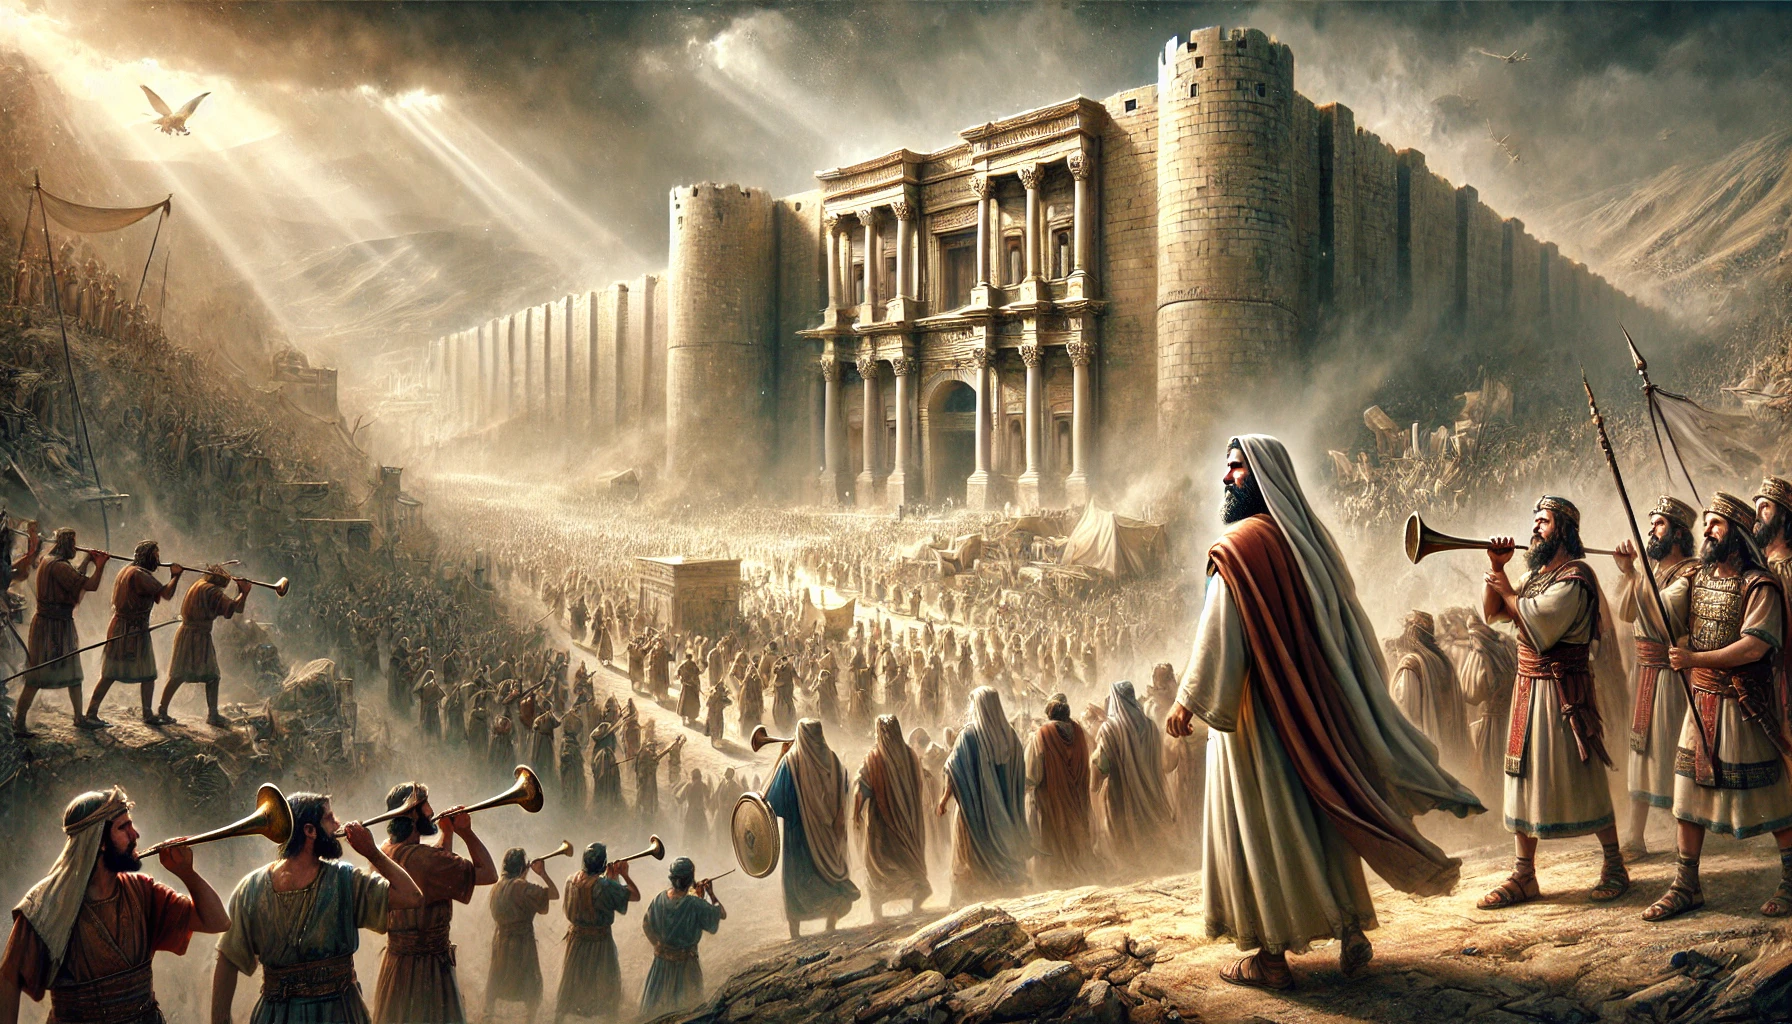
\includegraphics[width=0.7\linewidth]{graficas/josue.png}\\
	Josué y los Israelitas ante las murallas de Jericó\\
\end{center}




\section*{Capítulo 1 }
Preparativos para la conquista  
1:1 Aconteció después de la muerte de Moisés siervo de Jehová, que Jehová habló a Josué hijo de Nun, servidor de Moisés, diciendo:  
1:2 Mi siervo Moisés ha muerto; ahora, pues, levántate y pasa este Jordán, tú y todo este pueblo, a la tierra que yo les doy a los hijos de Israel.  
1:3 Yo os he entregado, como lo había dicho a Moisés, todo lugar que pisare la planta de vuestro pie.  
1:4 Desde el desierto y el Líbano hasta el gran río Eufrates, toda la tierra de los heteos hasta el gran mar donde se pone el sol, será vuestro territorio.  
1:5 Nadie te podrá hacer frente en todos los días de tu vida; como estuve con Moisés, estaré contigo; no te dejaré, ni te desampararé.  
1:6 Esfuérzate y sé valiente; porque tú repartirás a este pueblo por heredad la tierra de la cual juré a sus padres que la daría a ellos.  
1:7 Solamente esfuérzate y sé muy valiente, para cuidar de hacer conforme a toda la ley que mi siervo Moisés te mandó; no te apartes de ella ni a diestra ni a siniestra, para que seas prosperado en todas las cosas que emprendas.  
1:8 Nunca se apartará de tu boca este libro de la ley, sino que de día y de noche meditarás en él, para que guardes y hagas conforme a todo lo que en él está escrito; porque entonces harás prosperar tu camino, y todo te saldrá bien.  
1:9 Mira que te mando que te esfuerces y seas valiente; no temas ni desmayes, porque Jehová tu Dios estará contigo en dondequiera que vayas.  
1:10 Y Josué mandó a los oficiales del pueblo, diciendo:  
1:11 Pasad por en medio del campamento y mandad al pueblo, diciendo: Preparaos comida, porque dentro de tres días pasaréis el Jordán para entrar a poseer la tierra que Jehová vuestro Dios os da en posesión.  
1:12 También habló Josué a los rubenitas y gaditas y a la media tribu de Manasés, diciendo:  
1:13 Acordaos de la palabra que Moisés, siervo de Jehová, os mandó diciendo: Jehová vuestro Dios os ha dado reposo, y os ha dado esta tierra.  
1:14 Vuestras mujeres, vuestros niños y vuestros ganados quedarán en la tierra que Moisés os ha dado a este lado del Jordán; mas vosotros, todos los valientes y fuertes, pasaréis armados delante de vuestros hermanos, y les ayudaréis,  
1:15 hasta tanto que Jehová haya dado reposo a vuestros hermanos como a vosotros, y que ellos también posean la tierra que Jehová vuestro Dios les da; y después volveréis vosotros a la tierra de vuestra herencia, la cual Moisés siervo de Jehová os ha dado, a este lado del Jordán hacia donde nace el sol; y entraréis en posesión de ella. 
1:16 Entonces respondieron a Josué, diciendo: Nosotros haremos todas las cosas que nos has mandado, e iremos adondequiera que nos mandes.  
1:17 De la manera que obedecimos a Moisés en todas las cosas, así te obedeceremos a ti; solamente que Jehová tu Dios esté contigo, como estuvo con Moisés.  
1:18 Cualquiera que fuere rebelde a tu mandamiento, y no obedeciere a tus palabras en todas las cosas que le mandes, que muera; solamente que te esfuerces y seas valiente.  
\section*{Capítulo 2}
Josué envía espías a Jericó  

2:1 Josué hijo de Nun envió desde Sitim dos espías secretamente, diciéndoles: Andad, reconoced la tierra, y a Jericó. Y ellos fueron, y entraron en casa de una ramera que se llamaba Rahab, y posaron allí.  
2:2 Y fue dado aviso al rey de Jericó, diciendo: He aquí que hombres de los hijos de Israel han venido aquí esta noche para espiar la tierra.  
2:3 Entonces el rey de Jericó envió a decir a Rahab: Saca a los hombres que han venido a ti, y han entrado a tu casa; porque han venido para espiar toda la tierra.  
2:4 Pero la mujer había tomado a los dos hombres y los había escondido; y dijo: Es verdad que unos hombres vinieron a mí, pero no supe de dónde eran.  
2:5 Y cuando se iba a cerrar la puerta, siendo ya oscuro, esos hombres se salieron, y no sé a dónde han ido; seguidlos aprisa, y los alcanzaréis.  
2:6 Mas ella los había hecho subir al terrado, y los había escondido entre los manojos de lino que tenía puestos en el terrado.  
2:7 Y los hombres fueron tras ellos por el camino del Jordán, hasta los vados; y la puerta fue cerrada después que salieron los perseguidores.  
2:8 Antes que ellos se durmiesen, ella subió al terrado, y les dijo:  
2:9 Sé que Jehová os ha dado esta tierra; porque el temor de vosotros ha caído sobre nosotros, y todos los moradores del país ya han desmayado por causa de vosotros.  
2:10 Porque hemos oído que Jehová hizo secar las aguas del Mar Rojo delante de vosotros cuando salisteis de Egipto, y lo que habéis hecho a los dos reyes de los amorreos que estaban al otro lado del Jordán, a Sehón y a Og, a los cuales habéis destruido. 
2:11 Oyendo esto, ha desmayado nuestro corazón; ni ha quedado más aliento en hombre alguno por causa de vosotros, porque Jehová vuestro Dios es Dios arriba en los cielos y abajo en la tierra.  
2:12 Os ruego pues, ahora, que me juréis por Jehová, que como he hecho misericordia con vosotros, así la haréis vosotros con la casa de mi padre, de lo cual me daréis una señal segura;  
2:13 y que salvaréis la vida a mi padre y a mi madre, a mis hermanos y hermanas, y a todo lo que es suyo; y que libraréis nuestras vidas de la muerte.  
2:14 Ellos le respondieron: Nuestra vida responderá por la vuestra, si no denunciareis este asunto nuestro; y cuando Jehová nos haya dado la tierra, nosotros haremos contigo misericordia y verdad.  
2:15 Entonces ella los hizo descender con una cuerda por la ventana; porque su casa estaba en el muro de la ciudad, y ella vivía en el muro.  
2:16 Y les dijo: Marchaos al monte, para que los que fueron tras vosotros no os encuentren; y estad escondidos allí tres días, hasta que los que os siguen hayan vuelto; y después os iréis por vuestro camino.  
2:17 Y ellos le dijeron: Nosotros quedaremos libres de este juramento con que nos has juramentado.  
2:18 He aquí, cuando nosotros entremos en la tierra, tú atarás este cordón de grana a la ventana por la cual nos descolgaste; y reunirás en tu casa a tu padre y a tu madre, a tus hermanos y a toda la familia de tu padre.  
2:19 Cualquiera que saliere fuera de las puertas de tu casa, su sangre será sobre su cabeza, y nosotros sin culpa. Mas cualquiera que se estuviere en casa contigo, su sangre será sobre nuestra cabeza, si mano le tocare.  
2:20 Y si tú denunciares este nuestro asunto, nosotros quedaremos libres de este tu juramento con que nos has juramentado.  
2:21 Ella respondió: Sea así como habéis dicho. Luego los despidió, y se fueron; y ella ató el cordón de grana a la ventana.  
2:22 Y caminando ellos, llegaron al monte y estuvieron allí tres días, hasta que volvieron los que los perseguían; y los que los persiguieron buscaron por todo el camino, pero no los hallaron.  
2:23 Entonces volvieron los dos hombres; descendieron del monte, y pasaron, y vinieron a Josué hijo de Nun, y le contaron todas las cosas que les habían acontecido.  
2:24 Y dijeron a Josué: Jehová ha entregado toda la tierra en nuestras manos; y también todos los moradores del país desmayan delante de nosotros.  
\section*{Capítulo 3}
El paso del Jordán  

3:1 Josué se levantó de mañana, y él y todos los hijos de Israel partieron de Sitim y vinieron hasta el Jordán, y reposaron allí antes de pasarlo.  
3:2 Y después de tres días, los oficiales recorrieron el campamento,  
3:3 y mandaron al pueblo, diciendo: Cuando veáis el arca del pacto de Jehová vuestro Dios, y los levitas sacerdotes que la llevan, vosotros saldréis de vuestro lugar y marcharéis en pos de ella,  
3:4 a fin de que sepáis el camino por donde habéis de ir; por cuanto vosotros no habéis pasado antes de ahora por este camino. Pero entre vosotros y ella haya distancia como de dos mil codos; no os acercaréis a ella.  
3:5 Y Josué dijo al pueblo: Santificaos, porque Jehová hará mañana maravillas entre vosotros.  
3:6 Y habló Josué a los sacerdotes, diciendo: Tomad el arca del pacto, y pasad delante del pueblo. Y ellos tomaron el arca del pacto y fueron delante del pueblo.  
3:7 Entonces Jehová dijo a Josué: Desde este día comenzaré a engrandecerte delante de los ojos de todo Israel, para que entiendan que como estuve con Moisés, así estaré contigo.  
3:8 Tú, pues, mandarás a los sacerdotes que llevan el arca del pacto, diciendo: Cuando hayáis entrado hasta el borde del agua del Jordán, pararéis en el Jordán.  
3:9 Y Josué dijo a los hijos de Israel: Acercaos, y escuchad las palabras de Jehová vuestro Dios.  
3:10 Y añadió Josué: En esto conoceréis que el Dios viviente está en medio de vosotros, y que él echará de delante de vosotros al cananeo, al heteo, al heveo, al ferezeo, al gergeseo, al amorreo y al jebuseo.  
3:11 He aquí, el arca del pacto del Señor de toda la tierra pasará delante de vosotros en medio del Jordán.  
3:12 Tomad, pues, ahora doce hombres de las tribus de Israel, uno de cada tribu.  
3:13 Y cuando las plantas de los pies de los sacerdotes que llevan el arca de Jehová, Señor de toda la tierra, se asienten en las aguas del Jordán, las aguas del Jordán se dividirán; porque las aguas que vienen de arriba se detendrán en un montón.  
3:14 Y aconteció cuando partió el pueblo de sus tiendas para pasar el Jordán, con los sacerdotes delante del pueblo llevando el arca del pacto,  
3:15 cuando los que llevaban el arca entraron en el Jordán, y los pies de los sacerdotes que llevaban el arca fueron mojados a la orilla del agua (porque el Jordán suele desbordarse por todas sus orillas todo el tiempo de la siega),  
3:16 las aguas que venían de arriba se detuvieron como en un montón bien lejos de la ciudad de Adam, que está al lado de Saretán, y las que descendían al mar del Arabá, al Mar Salado, se acabaron, y fueron divididas; y el pueblo pasó en dirección de Jericó.  
3:17 Mas los sacerdotes que llevaban el arca del pacto de Jehová, estuvieron en seco, firmes en medio del Jordán, hasta que todo el pueblo hubo acabado de pasar el Jordán; y todo Israel pasó en seco.  
\section*{Capítulo 4}
Las doce piedras tomadas del Jordán  

4:1 Cuando toda la gente hubo acabado de pasar el Jordán, Jehová habló a Josué, diciendo:  
4:2 Tomad del pueblo doce hombres, uno de cada tribu,  
4:3 y mandadles, diciendo: Tomad de aquí de en medio del Jordán, del lugar donde están firmes los pies de los sacerdotes, doce piedras, las cuales pasaréis con vosotros, y levantadlas en el lugar donde habéis de pasar la noche.  
4:4 Entonces Josué llamó a los doce hombres a los cuales él había designado de entre los hijos de Israel, uno de cada tribu.  
4:5 Y les dijo Josué: Pasad delante del arca de Jehová vuestro Dios a la mitad del Jordán, y cada uno de vosotros tome una piedra sobre su hombro, conforme al número de las tribus de los hijos de Israel,  
4:6 para que esto sea señal entre vosotros; y cuando vuestros hijos preguntaren a sus padres mañana, diciendo: ¿Qué significan estas piedras?  
4:7 les responderéis: Que las aguas del Jordán fueron divididas delante del arca del pacto de Jehová; cuando ella pasó el Jordán, las aguas del Jordán se dividieron; y estas piedras servirán de monumento conmemorativo a los hijos de Israel para siempre.  
4:8 Y los hijos de Israel lo hicieron así como Josué les mandó: tomaron doce piedras de en medio del Jordán, como Jehová lo había dicho a Josué, conforme al número de las tribus de los hijos de Israel, y las pasaron al lugar donde acamparon, y las levantaron allí.  
4:9 Josué también levantó doce piedras en medio del Jordán, en el lugar donde estuvieron los pies de los sacerdotes que llevaban el arca del pacto; y han estado allí hasta hoy.  
4:10 Y los sacerdotes que llevaban el arca se pararon en medio del Jordán hasta que se hizo todo lo que Jehová había mandado a Josué que dijese al pueblo, conforme a todas las cosas que Moisés había mandado a Josué; y el pueblo se dio prisa y pasó.  
4:11 Y cuando todo el pueblo acabó de pasar, también pasó el arca de Jehová, y los sacerdotes, en presencia del pueblo.  
4:12 También los hijos de Rubén y los hijos de Gad y la media tribu de Manasés pasaron armados delante de los hijos de Israel, según Moisés les había dicho;  
4:13 como cuarenta mil hombres armados, listos para la guerra, pasaron hacia la llanura de Jericó delante de Jehová.  
4:14 En aquel día Jehová engrandeció a Josué a los ojos de todo Israel; y le temieron, como habían temido a Moisés, todos los días de su vida.  
4:15 Luego Jehová habló a Josué, diciendo:  
4:16 Manda a los sacerdotes que llevan el arca del testimonio, que suban del Jordán.  
4:17 Y Josué mandó a los sacerdotes, diciendo: Subid del Jordán.  
4:18 Y aconteció que cuando los sacerdotes que llevaban el arca del pacto de Jehová subieron de en medio del Jordán, y las plantas de los pies de los sacerdotes estuvieron en lugar seco, las aguas del Jordán se volvieron a su lugar, corriendo como antes sobre todos sus bordes.  
4:19 Y el pueblo subió del Jordán el día diez del mes primero, y acamparon en Gilgal, al lado oriental de Jericó.  
4:20 Y Josué erigió en Gilgal las doce piedras que habían traído del Jordán.  
4:21 Y habló a los hijos de Israel, diciendo: Cuando mañana preguntaren vuestros hijos a sus padres, y dijeren: ¿Qué significan estas piedras?  
4:22 declararéis a vuestros hijos, diciendo: Israel pasó en seco por este Jordán.  
4:23 Porque Jehová vuestro Dios secó las aguas del Jordán delante de vosotros, hasta que habíais pasado, a la manera que Jehová vuestro Dios lo había hecho en el Mar Rojo, el cual secó delante de nosotros hasta que pasamos;  
4:24 para que todos los pueblos de la tierra conozcan que la mano de Jehová es poderosa; para que temáis a Jehová vuestro Dios todos los días.  
\section*{Capítulo 5 }
La circuncisión y la pascua en Gilgal  

5:1 Cuando todos los reyes de los amorreos que estaban al otro lado del Jordán al occidente, y todos los reyes de los cananeos que estaban cerca del mar, oyeron cómo Jehová había secado las aguas del Jordán delante de los hijos de Israel hasta que hubieron pasado, desfalleció su corazón, y no hubo más aliento en ellos delante de los hijos de Israel.  
5:2 En aquel tiempo Jehová dijo a Josué: Hazte cuchillos afilados, y vuelve a circuncidar la segunda vez a los hijos de Israel.  
5:3 Y Josué se hizo cuchillos afilados, y circuncidó a los hijos de Israel en el collado de Aralot.  
5:4 Esta es la causa por la cual Josué los circuncidó: Todo el pueblo que había salido de Egipto, los varones, todos los hombres de guerra, habían muerto en el desierto, por el camino, después que salieron de Egipto.  
5:5 Pues todos los del pueblo que habían salido, estaban circuncidados; mas todo el pueblo que había nacido en el desierto, por el camino, después que hubieron salido de Egipto, no estaba circuncidado.  
5:6 Porque los hijos de Israel anduvieron por el desierto cuarenta años, hasta que todos los hombres de guerra que habían salido de Egipto fueron consumidos, por cuanto no obedecieron a la voz de Jehová; por lo cual Jehová les juró que no les dejaría ver la tierra de la cual Jehová había jurado a sus padres que nos la daría, tierra que fluye leche y miel. 
5:7 A los hijos de ellos, que él había hecho suceder en su lugar, Josué los circuncidó; pues eran incircuncisos, porque no habían sido circuncidados por el camino.  
5:8 Y cuando acabaron de circuncidar a toda la gente, se quedaron en el mismo lugar en el campamento, hasta que sanaron.  
5:9 Y Jehová dijo a Josué: Hoy he quitado de vosotros el oprobio de Egipto; por lo cual el nombre de aquel lugar fue llamado Gilgal, hasta hoy.  
5:10 Y los hijos de Israel acamparon en Gilgal, y celebraron la pascua a los catorce días del mes, por la tarde, en los llanos de Jericó.  
5:11 Al otro día de la pascua comieron del fruto de la tierra, los panes sin levadura, y en el mismo día espigas nuevas tostadas.  
5:12 Y el maná cesó el día siguiente, desde que comenzaron a comer del fruto de la tierra; y los hijos de Israel nunca más tuvieron maná, sino que comieron de los frutos de la tierra de Canaán aquel año.  
Josué y el varón con la espada desenvainada  
5:13 Estando Josué cerca de Jericó, alzó sus ojos y vio un varón que estaba delante de él, el cual tenía una espada desenvainada en su mano. Y Josué, yendo hacia él, le dijo: ¿Eres de los nuestros, o de nuestros enemigos?  
5:14 El respondió: No; mas como Príncipe del ejército de Jehová he venido ahora. Entonces Josué, postrándose sobre su rostro en tierra, le adoró; y le dijo: ¿Qué dice mi Señor a su siervo?  
5:15 Y el Príncipe del ejército de Jehová respondió a Josué: Quita el calzado de tus pies, porque el lugar donde estás es santo. Y Josué así lo hizo.  
\section*{Capítulo 6 }
La toma de Jericó  

6:1 Ahora, Jericó estaba cerrada, bien cerrada, a causa de los hijos de Israel; nadie entraba ni salía.  
6:2 Mas Jehová dijo a Josué: Mira, yo he entregado en tu mano a Jericó y a su rey, con sus varones de guerra.  
6:3 Rodearéis, pues, la ciudad todos los hombres de guerra, yendo alrededor de la ciudad una vez; y esto haréis durante seis días.  
6:4 Y siete sacerdotes llevarán siete bocinas de cuernos de carnero delante del arca; y al séptimo día daréis siete vueltas a la ciudad, y los sacerdotes tocarán las bocinas.  
6:5 Y cuando toquen prolongadamente el cuerno de carnero, así que oigáis el sonido de la bocina, todo el pueblo gritará a gran voz, y el muro de la ciudad caerá; entonces subirá el pueblo, cada uno derecho hacia adelante.  
6:6 Llamando, pues, Josué hijo de Nun a los sacerdotes, les dijo: Llevad el arca del pacto, y siete sacerdotes lleven bocinas de cuerno de carnero delante del arca de Jehová.  
6:7 Y dijo al pueblo: Pasad, y rodead la ciudad; y los que están armados pasarán delante del arca de Jehová.  
6:8 Y así que Josué hubo hablado al pueblo, los siete sacerdotes, llevando las siete bocinas de cuerno de carnero, pasaron delante del arca de Jehová, y tocaron las bocinas; y el arca del pacto de Jehová los seguía.  
6:9 Y los hombres armados iban delante de los sacerdotes que tocaban las bocinas, y la retaguardia iba tras el arca, mientras las bocinas sonaban continuamente.  
6:10 Y Josué mandó al pueblo, diciendo: Vosotros no gritaréis, ni se oirá vuestra voz, ni saldrá palabra de vuestra boca, hasta el día que yo os diga: Gritad; entonces gritaréis.  
6:11 Así que él hizo que el arca de Jehová diera una vuelta alrededor de la ciudad, y volvieron luego al campamento, y allí pasaron la noche.  
6:12 Y Josué se levantó de mañana, y los sacerdotes tomaron el arca de Jehová.  
6:13 Y los siete sacerdotes, llevando las siete bocinas de cuerno de carnero, fueron delante del arca de Jehová, andando siempre y tocando las bocinas; y los hombres armados iban delante de ellos, y la retaguardia iba tras el arca de Jehová, mientras las bocinas tocaban continuamente.  
6:14 Así dieron otra vuelta a la ciudad el segundo día, y volvieron al campamento; y de esta manera hicieron durante seis días.  
6:15 Al séptimo día se levantaron al despuntar el alba, y dieron vuelta a la ciudad de la misma manera siete veces; solamente este día dieron vuelta alrededor de ella siete veces.  
6:16 Y cuando los sacerdotes tocaron las bocinas la séptima vez, Josué dijo al pueblo: Gritad, porque Jehová os ha entregado la ciudad.  
6:17 Y será la ciudad anatema a Jehová, con todas las cosas que están en ella; solamente Rahab la ramera vivirá, con todos los que estén en casa con ella, por cuanto escondió a los mensajeros que enviamos.  
6:18 Pero vosotros guardaos del anatema; ni toquéis, ni toméis alguna cosa del anatema, no sea que hagáis anatema el campamento de Israel, y lo turbéis.  
6:19 Mas toda la plata y el oro, y los utensilios de bronce y de hierro, sean consagrados a Jehová, y entren en el tesoro de Jehová.  
6:20 Entonces el pueblo gritó, y los sacerdotes tocaron las bocinas; y aconteció que cuando el pueblo hubo oído el sonido de la bocina, gritó con gran vocerío, y el muro se derrumbó. El pueblo subió luego a la ciudad, cada uno derecho hacia adelante, y la tomaron.  
6:21 Y destruyeron a filo de espada todo lo que en la ciudad había; hombres y mujeres, jóvenes y viejos, hasta los bueyes, las ovejas, y los asnos.  
6:22 Mas Josué dijo a los dos hombres que habían reconocido la tierra: Entrad en casa de la mujer ramera, y haced salir de allí a la mujer y a todo lo que fuere suyo, como lo jurasteis.  
6:23 Y los espías entraron y sacaron a Rahab, a su padre, a su madre, a sus hermanos y todo lo que era suyo; y también sacaron a toda su parentela, y los pusieron fuera del campamento de Israel.  
6:24 Y consumieron con fuego la ciudad, y todo lo que en ella había; solamente pusieron en el tesoro de la casa de Jehová la plata y el oro, y los utensilios de bronce y de hierro.  
6:25 Mas Josué salvó la vida a Rahab la ramera, y a la casa de su padre, y a todo lo que ella tenía; y habitó ella entre los israelitas hasta hoy, por cuanto escondió a los mensajeros que Josué había enviado a reconocer a Jericó. 
6:26 En aquel tiempo hizo Josué un juramento, diciendo: Maldito delante de Jehová el hombre que se levantare y reedificare esta ciudad de Jericó. Sobre su primogénito eche los cimientos de ella, y sobre su hijo menor asiente sus puertas. 
6:27 Estaba, pues, Jehová con Josué, y su nombre se divulgó por toda la tierra.  
\section*{Capítulo 7 }
El pecado de Acán  

7:1 Pero los hijos de Israel cometieron una prevaricación en cuanto al anatema; porque Acán hijo de Carmi, hijo de Zabdi, hijo de Zera, de la tribu de Judá, tomó del anatema; y la ira de Jehová se encendió contra los hijos de Israel.  
7:2 Después Josué envió hombres desde Jericó a Hai, que estaba junto a Bet-avén hacia el oriente de Bet-el; y les habló diciendo: Subid y reconoced la tierra. Y ellos subieron y reconocieron a Hai.  
7:3 Y volviendo a Josué, le dijeron: No suba todo el pueblo, sino suban como dos mil o tres mil hombres, y tomarán a Hai; no fatigues a todo el pueblo yendo allí, porque son pocos.  
7:4 Y subieron allá del pueblo como tres mil hombres, los cuales huyeron delante de los de Hai.  
7:5 Y los de Hai mataron de ellos a unos treinta y seis hombres, y los siguieron desde la puerta hasta Sebarim, y los derrotaron en la bajada; por lo cual el corazón del pueblo desfalleció y vino a ser como agua.  
7:6 Entonces Josué rompió sus vestidos, y se postró en tierra sobre su rostro delante del arca de Jehová hasta caer la tarde, él y los ancianos de Israel; y echaron polvo sobre sus cabezas.  
7:7 Y Josué dijo: ¡Ah, Señor Jehová! ¿Por qué hiciste pasar a este pueblo el Jordán, para entregarnos en las manos de los amorreos, para que nos destruyan? ¡Ojalá nos hubiéramos quedado al otro lado del Jordán!  
7:8 ¡Ay, Señor! ¿qué diré, ya que Israel ha vuelto la espalda delante de sus enemigos?  
7:9 Porque los cananeos y todos los moradores de la tierra oirán, y nos rodearán, y borrarán nuestro nombre de sobre la tierra; y entonces, ¿qué harás tú a tu grande nombre?  
7:10 Y Jehová dijo a Josué: Levántate; ¿por qué te postras así sobre tu rostro?  
7:11 Israel ha pecado, y aun han quebrantado mi pacto que yo les mandé; y también han tomado del anatema, y hasta han hurtado, han mentido, y aun lo han guardado entre sus enseres.  
7:12 Por esto los hijos de Israel no podrán hacer frente a sus enemigos, sino que delante de sus enemigos volverán la espalda, por cuanto han venido a ser anatema; ni estaré más con vosotros, si no destruyereis el anatema de en medio de vosotros.  
7:13 Levántate, santifica al pueblo, y di: Santificaos para mañana; porque Jehová el Dios de Israel dice así: Anatema hay en medio de ti, Israel; no podrás hacer frente a tus enemigos, hasta que hayáis quitado el anatema de en medio de vosotros.  
7:14 Os acercaréis, pues, mañana por vuestras tribus; y la tribu que Jehová tomare, se acercará por sus familias; y la familia que Jehová tomare, se acercará por sus casas; y la casa que Jehová tomare, se acercará por los varones;  
7:15 y el que fuere sorprendido en el anatema, será quemado, él y todo lo que tiene, por cuanto ha quebrantado el pacto de Jehová, y ha cometido maldad en Israel.  
7:16 Josué, pues, levantándose de mañana, hizo acercar a Israel por sus tribus; y fue tomada la tribu de Judá.  
7:17 Y haciendo acercar a la tribu de Judá, fue tomada la familia de los de Zera; y haciendo luego acercar a la familia de los de Zera por los varones, fue tomado Zabdi.  
7:18 Hizo acercar su casa por los varones, y fue tomado Acán hijo de Carmi, hijo de Zabdi, hijo de Zera, de la tribu de Judá.  
7:19 Entonces Josué dijo a Acán: Hijo mío, da gloria a Jehová el Dios de Israel, y dale alabanza, y declárame ahora lo que has hecho; no me lo encubras.  
7:20 Y Acán respondió a Josué diciendo: Verdaderamente yo he pecado contra Jehová el Dios de Israel, y así y así he hecho.  
7:21 Pues vi entre los despojos un manto babilónico muy bueno, y doscientos siclos de plata, y un lingote de oro de peso de cincuenta siclos, lo cual codicié y tomé; y he aquí que está escondido bajo tierra en medio de mi tienda, y el dinero debajo de ello.  
7:22 Josué entonces envió mensajeros, los cuales fueron corriendo a la tienda; y he aquí estaba escondido en su tienda, y el dinero debajo de ello.  
7:23 Y tomándolo de en medio de la tienda, lo trajeron a Josué y a todos los hijos de Israel, y lo pusieron delante de Jehová. 
7:24 Entonces Josué, y todo Israel con él, tomaron a Acán hijo de Zera, el dinero, el manto, el lingote de oro, sus hijos, sus hijas, sus bueyes, sus asnos, sus ovejas, su tienda y todo cuanto tenía, y lo llevaron todo al valle de Acor.  
7:25 Y le dijo Josué: ¿Por qué nos has turbado? Túrbete Jehová en este día. Y todos los israelitas los apedrearon, y los quemaron después de apedrearlos.  
7:26 Y levantaron sobre él un gran montón de piedras, que permanece hasta hoy. Y Jehová se volvió del ardor de su ira. Y por esto aquel lugar se llama el Valle de Acor, hasta hoy.  
\section*{Capítulo 8}
Toma y destrucción de Hai  

8:1 Jehová dijo a Josué: No temas ni desmayes; toma contigo toda la gente de guerra, y levántate y sube a Hai. Mira, yo he entregado en tu mano al rey de Hai, a su pueblo, a su ciudad y a su tierra.  
8:2 Y harás a Hai y a su rey como hiciste a Jericó y a su rey; sólo que sus despojos y sus bestias tomaréis para vosotros. Pondrás, pues, emboscadas a la ciudad detrás de ella.  
8:3 Entonces se levantaron Josué y toda la gente de guerra, para subir contra Hai; y escogió Josué treinta mil hombres fuertes, los cuales envió de noche.  
8:4 Y les mandó, diciendo: Atended, pondréis emboscada a la ciudad detrás de ella; no os alejaréis mucho de la ciudad, y estaréis todos dispuestos.  
8:5 Y yo y todo el pueblo que está conmigo nos acercaremos a la ciudad; y cuando salgan ellos contra nosotros, como hicieron antes, huiremos delante de ellos.  
8:6 Y ellos saldrán tras nosotros, hasta que los alejemos de la ciudad; porque dirán: Huyen de nosotros como la primera vez. Huiremos, pues, delante de ellos.  
8:7 Entonces vosotros os levantaréis de la emboscada y tomaréis la ciudad; pues Jehová vuestro Dios la entregará en vuestras manos.  
8:8 Y cuando la hayáis tomado, le prenderéis fuego. Haréis conforme a la palabra de Jehová; mirad que os lo he mandado.  
8:9 Entonces Josué los envió; y ellos se fueron a la emboscada, y se pusieron entre Bet-el y Hai, al occidente de Hai; y Josué se quedó aquella noche en medio del pueblo.  
8:10 Levantándose Josué muy de mañana, pasó revista al pueblo, y subió él, con los ancianos de Israel, delante del pueblo contra Hai.  
8:11 Y toda la gente de guerra que con él estaba, subió y se acercó, y llegaron delante de la ciudad, y acamparon al norte de Hai; y el valle estaba entre él y Hai.  
8:12 Y tomó como cinco mil hombres, y los puso en emboscada entre Bet-el y Hai, al occidente de la ciudad.  
8:13 Así dispusieron al pueblo: todo el campamento al norte de la ciudad, y su emboscada al occidente de la ciudad, y Josué avanzó aquella noche hasta la mitad del valle.  
8:14 Y aconteció que viéndolo el rey de Hai, él y su pueblo se apresuraron y madrugaron; y al tiempo señalado, los hombres de la ciudad salieron al encuentro de Israel para combatir, frente al Arabá, no sabiendo que estaba puesta emboscada a espaldas de la ciudad.  
8:15 Entonces Josué y todo Israel se fingieron vencidos y huyeron delante de ellos por el camino del desierto.  
8:16 Y todo el pueblo que estaba en Hai se juntó para seguirles; y siguieron a Josué, siendo así alejados de la ciudad. 
8:17 Y no quedó hombre en Hai ni en Bet-el, que no saliera tras de Israel; y por seguir a Israel dejaron la ciudad abierta.  
8:18 Entonces Jehová dijo a Josué: Extiende la lanza que tienes en tu mano hacia Hai, porque yo la entregaré en tu mano. Y Josué extendió hacia la ciudad la lanza que en su mano tenía.  
8:19 Y levantándose prontamente de su lugar los que estaban en la emboscada, corrieron luego que él alzó su mano, y vinieron a la ciudad, y la tomaron, y se apresuraron a prenderle fuego.  
8:20 Y los hombres de Hai volvieron el rostro, y al mirar, he aquí que el humo de la ciudad subía al cielo, y no pudieron huir ni a una parte ni a otra, porque el pueblo que iba huyendo hacia el desierto se volvió contra los que les seguían.  
8:21 Josué y todo Israel, viendo que los de la emboscada habían tomado la ciudad, y que el humo de la ciudad subía, se volvieron y atacaron a los de Hai.  
8:22 Y los otros salieron de la ciudad a su encuentro, y así fueron encerrados en medio de Israel, los unos por un lado, y los otros por el otro. Y los hirieron hasta que no quedó ninguno de ellos que escapase.  
8:23 Pero tomaron vivo al rey de Hai, y lo trajeron a Josué.  
8:24 Y cuando los israelitas acabaron de matar a todos los moradores de Hai en el campo y en el desierto a donde los habían perseguido, y todos habían caído a filo de espada hasta ser consumidos, todos los israelitas volvieron a Hai, y también la hirieron a filo de espada.  
8:25 Y el número de los que cayeron aquel día, hombres y mujeres, fue de doce mil, todos los de Hai.  
8:26 Porque Josué no retiró su mano que había extendido con la lanza, hasta que hubo destruido por completo a todos los moradores de Hai.  
8:27 Pero los israelitas tomaron para sí las bestias y los despojos de la ciudad, conforme a la palabra de Jehová que le había mandado a Josué.  
8:28 Y Josué quemó a Hai y la redujo a un montón de escombros, asolada para siempre hasta hoy.  
8:29 Y al rey de Hai lo colgó de un madero hasta caer la noche; y cuando el sol se puso, mandó Josué que quitasen del madero su cuerpo, y lo echasen a la puerta de la ciudad; y levantaron sobre él un gran montón de piedras, que permanece hasta hoy.  
Lectura de la ley en el Monte Ebal  
8:30 Entonces Josué edificó un altar a Jehová Dios de Israel en el monte Ebal,  
8:31 como Moisés siervo de Jehová lo había mandado a los hijos de Israel, como está escrito en el libro de la ley de Moisés, un altar de piedras enteras sobre las cuales nadie alzó hierro; y ofrecieron sobre él holocaustos a Jehová, y sacrificaron ofrendas de paz.  
8:32 También escribió allí sobre las piedras una copia de la ley de Moisés, la cual escribió delante de los hijos de Israel. 
8:33 Y todo Israel, con sus ancianos, oficiales y jueces, estaba de pie a uno y otro lado del arca, en presencia de los sacerdotes levitas que llevaban el arca del pacto de Jehová, así los extranjeros como los naturales. La mitad de ellos estaba hacia el monte Gerizim, y la otra mitad hacia el monte Ebal, de la manera que Moisés, siervo de Jehová, lo había mandado antes, para que bendijesen primeramente al pueblo de Israel.  
8:34 Después de esto, leyó todas las palabras de la ley, las bendiciones y las maldiciones, conforme a todo lo que está escrito en el libro de la ley.  
8:35 No hubo palabra alguna de todo cuanto mandó Moisés, que Josué no hiciese leer delante de toda la congregación de Israel, y de las mujeres, de los niños, y de los extranjeros que moraban entre ellos. 
\section*{Capítulo 9 }
Astucia de los gabaonitas  

9:1 Cuando oyeron estas cosas todos los reyes que estaban a este lado del Jordán, así en las montañas como en los llanos, y en toda la costa del Mar Grande delante del Líbano, los heteos, amorreos, cananeos, ferezeos, heveos y jebuseos,  
9:2 se concertaron para pelear contra Josué e Israel.  
9:3 Mas los moradores de Gabaón, cuando oyeron lo que Josué había hecho a Jericó y a Hai,  
9:4 usaron de astucia; pues fueron y se fingieron embajadores, y tomaron sacos viejos sobre sus asnos, y cueros viejos de vino, rotos y remendados,  
9:5 y zapatos viejos y recosidos en sus pies, con vestidos viejos sobre sí; y todo el pan que traían para el camino era seco y mohoso.  
9:6 Y vinieron a Josué al campamento en Gilgal, y le dijeron a él y a los de Israel: Nosotros venimos de tierra muy lejana; haced, pues, ahora alianza con nosotros.  
9:7 Y los de Israel respondieron a los heveos: Quizás habitáis en medio de nosotros. ¿Cómo, pues, podremos hacer alianza con vosotros?  
9:8 Ellos respondieron a Josué: Nosotros somos tus siervos. Y Josué les dijo: ¿Quiénes sois vosotros, y de dónde venís?  
9:9 Y ellos respondieron: Tus siervos han venido de tierra muy lejana, por causa del nombre de Jehová tu Dios; porque hemos oído su fama, y todo lo que hizo en Egipto,  
9:10 y todo lo que hizo a los dos reyes de los amorreos que estaban al otro lado del Jordán: a Sehón rey de Hesbón, y a Og rey de Basán, que estaba en Astarot. 
9:11 Por lo cual nuestros ancianos y todos los moradores de nuestra tierra nos dijeron: Tomad en vuestras manos provisión para el camino, e id al encuentro de ellos, y decidles: Nosotros somos vuestros siervos; haced ahora alianza con nosotros.  
9:12 Este nuestro pan lo tomamos caliente de nuestras casas para el camino el día que salimos para venir a vosotros; y helo aquí ahora ya seco y mohoso.  
9:13 Estos cueros de vino también los llenamos nuevos; helos aquí ya rotos; también estos nuestros vestidos y nuestros zapatos están ya viejos a causa de lo muy largo del camino.  
9:14 Y los hombres de Israel tomaron de la provisiones de ellos, y no consultaron a Jehová.  
9:15 Y Josué hizo paz con ellos, y celebró con ellos alianza concediéndoles la vida; y también lo juraron los príncipes de la congregación.  
9:16 Pasados tres días después que hicieron alianza con ellos, oyeron que eran sus vecinos, y que habitaban en medio de ellos.  
9:17 Y salieron los hijos de Israel, y al tercer día llegaron a las ciudades de ellos; y sus ciudades eran Gabaón, Cafira, Beerot y Quiriat-jearim.  
9:18 Y no los mataron los hijos de Israel, por cuanto los príncipes de la congregación les habían jurado por Jehová el Dios de Israel. Y toda la congregación murmuraba contra los príncipes.  
9:19 Mas todos los príncipes respondieron a toda la congregación: Nosotros les hemos jurado por Jehová Dios de Israel; por tanto, ahora no les podemos tocar.  
9:20 Esto haremos con ellos: les dejaremos vivir, para que no venga ira sobre nosotros por causa del juramento que les hemos hecho.  
9:21 Dijeron, pues, de ellos los príncipes: Dejadlos vivir; y fueron constituidos leñadores y aguadores para toda la congregación, concediéndoles la vida, según les habían prometido los príncipes.  
9:22 Y llamándolos Josué, les habló diciendo: ¿Por qué nos habéis engañado, diciendo: Habitamos muy lejos de vosotros, siendo así que moráis en medio de nosotros?  
9:23 Ahora, pues, malditos sois, y no dejará de haber de entre vosotros siervos, y quien corte la leña y saque el agua para la casa de mi Dios.  
9:24 Y ellos respondieron a Josué y dijeron: Como fue dado a entender a tus siervos que Jehová tu Dios había mandado a Moisés su siervo que os había de dar toda la tierra, y que había de destruir a todos los moradores de la tierra delante de vosotros, por esto temimos en gran manera por nuestras vidas a causa de vosotros, e hicimos esto.  
9:25 Ahora, pues, henos aquí en tu mano; lo que te pareciere bueno y recto hacer de nosotros, hazlo.  
9:26 Y él lo hizo así con ellos; pues los libró de la mano de los hijos de Israel, y no los mataron.  
9:27 Y Josué los destinó aquel día a ser leñadores y aguadores para la congregación, y para el altar de Jehová en el lugar que Jehová eligiese, lo que son hasta hoy.  
\section*{Capítulo 10}
Derrota de los amorreos  

10:1 Cuando Adonisedec rey de Jerusalén oyó que Josué había tomado a Hai, y que la había asolado (como había hecho a Jericó y a su rey, así hizo a Hai y a su rey), y que los moradores de Gabaón habían hecho paz con los israelitas, y que estaban entre ellos,  
10:2 tuvo gran temor; porque Gabaón era una gran ciudad, como una de las ciudades reales, y mayor que Hai, y todos sus hombres eran fuertes.  
10:3 Por lo cual Adonisedec rey de Jerusalén envió a Hoham rey de Hebrón, a Piream rey de Jarmut, a Jafía rey de Laquis y a Debir rey de Eglón, diciendo:  
10:4 Subid a mí y ayudadme, y combatamos a Gabaón; porque ha hecho paz con Josué y con los hijos de Israel.  
10:5 Y cinco reyes de los amorreos, el rey de Jerusalén, el rey de Hebrón, el rey de Jarmut, el rey de Laquis y el rey de Eglón, se juntaron y subieron, ellos con todos sus ejércitos, y acamparon cerca de Gabaón, y pelearon contra ella.  
10:6 Entonces los moradores de Gabaón enviaron a decir a Josué al campamento en Gilgal: No niegues ayuda a tus siervos; sube prontamente a nosotros para defendernos y ayudarnos; porque todos los reyes de los amorreos que habitan en las montañas se han unido contra nosotros.  
10:7 Y subió Josué de Gilgal, él y todo el pueblo de guerra con él, y todos los hombres valientes.  
10:8 Y Jehová dijo a Josué: No tengas temor de ellos; porque yo los he entregado en tu mano, y ninguno de ellos prevalecerá delante de ti.  
10:9 Y Josué vino a ellos de repente, habiendo subido toda la noche desde Gilgal.  
10:10 Y Jehová los llenó de consternación delante de Israel, y los hirió con gran mortandad en Gabaón; y los siguió por el camino que sube a Bet-horón, y los hirió hasta Azeca y Maceda.  
10:11 Y mientras iban huyendo de los israelitas, a la bajada de Bet-horón, Jehová arrojó desde el cielo grandes piedras sobre ellos hasta Azeca, y murieron; y fueron más los que murieron por las piedras del granizo, que los que los hijos de Israel mataron a espada.  
10:12 Entonces Josué habló a Jehová el día en que Jehová entregó al amorreo delante de los hijos de Israel, y dijo en presencia de los israelitas:  
Sol, detente en Gabaón;  
Y tú, luna, en el valle de Ajalón. 
10:13 Y el sol se detuvo y la luna se paró,  
Hasta que la gente se hubo vengado de sus enemigos.  
¿No está escrito esto en el libro de Jaser? Y el sol se paró en medio del cielo, y no se apresuró a ponerse casi un día entero.  
10:14 Y no hubo día como aquel, ni antes ni después de él, habiendo atendido Jehová a la voz de un hombre; porque Jehová peleaba por Israel.  
10:15 Y Josué, y todo Israel con él, volvió al campamento en Gilgal.  
10:16 Y los cinco reyes huyeron, y se escondieron en una cueva en Maceda.  
10:17 Y fue dado aviso a Josué que los cinco reyes habían sido hallados escondidos en una cueva en Maceda.  
10:18 Entonces Josué dijo: Rodad grandes piedras a la entrada de la cueva, y poned hombres junto a ella para que los guarden;  
10:19 y vosotros no os detengáis, sino seguid a vuestros enemigos, y heridles la retaguardia, sin dejarles entrar en sus ciudades; porque Jehová vuestro Dios los ha entregado en vuestra mano.  
10:20 Y aconteció que cuando Josué y los hijos de Israel acabaron de herirlos con gran mortandad hasta destruirlos, los que quedaron de ellos se metieron en las ciudades fortificadas.  
10:21 Todo el pueblo volvió sano y salvo a Josué, al campamento en Maceda; no hubo quien moviese su lengua contra ninguno de los hijos de Israel.  
10:22 Entonces dijo Josué: Abrid la entrada de la cueva, y sacad de ella a esos cinco reyes.  
10:23 Y lo hicieron así, y sacaron de la cueva a aquellos cinco reyes: al rey de Jerusalén, al rey de Hebrón, al rey de Jarmut, al rey de Laquis y al rey de Eglón.  
10:24 Y cuando los hubieron llevado a Josué, llamó Josué a todos los varones de Israel, y dijo a los principales de la gente de guerra que habían venido con él: Acercaos, y poned vuestros pies sobre los cuellos de estos reyes. Y ellos se acercaron y pusieron sus pies sobre los cuellos de ellos.  
10:25 Y Josué les dijo: No temáis, ni os atemoricéis; sed fuertes y valientes, porque así hará Jehová a todos vuestros enemigos contra los cuales peleáis.  
10:26 Y después de esto Josué los hirió y los mató, y los hizo colgar en cinco maderos; y quedaron colgados en los maderos hasta caer la noche.  
10:27 Y cuando el sol se iba a poner, mandó Josué que los quitasen de los maderos, y los echasen en la cueva donde se habían escondido; y pusieron grandes piedras a la entrada de la cueva, las cuales permanecen hasta hoy.  
10:28 En aquel mismo día tomó Josué a Maceda, y la hirió a filo de espada, y mató a su rey; por completo los destruyó, con todo lo que en ella tenía vida, sin dejar nada; e hizo al rey de Maceda como había hecho al rey de Jericó.  
10:29 Y de Maceda pasó Josué, y todo Israel con él, a Libna; y peleó contra Libna;  
10:30 y Jehová la entregó también a ella y a su rey en manos de Israel; y la hirió a filo de espada, con todo lo que en ella tenía vida, sin dejar nada; e hizo a su rey de la manera como había hecho al rey de Jericó.  
10:31 Y Josué, y todo Israel con él, pasó de Libna a Laquis, y acampó cerca de ella, y la combatió;  
10:32 y Jehová entregó a Laquis en mano de Israel, y la tomó al día siguiente, y la hirió a filo de espada, con todo lo que en ella tenía vida, así como había hecho en Libna.  
10:33 Entonces Horam rey de Gezer subió en ayuda de Laquis; mas a él y a su pueblo destruyó Josué, hasta no dejar a ninguno de ellos.  
10:34 De Laquis pasó Josué, y todo Israel con él, a Eglón; y acamparon cerca de ella, y la combatieron;  
10:35 y la tomaron el mismo día, y la hirieron a filo de espada; y aquel día mató a todo lo que en ella tenía vida, como había hecho en Laquis.  
10:36 Subió luego Josué, y todo Israel con él, de Eglón a Hebrón, y la combatieron.  
10:37 Y tomándola, la hirieron a filo de espada, a su rey y a todas sus ciudades, con todo lo que en ella tenía vida, sin dejar nada; como había hecho a Eglón, así la destruyeron con todo lo que en ella tenía vida.  
10:38 Después volvió Josué, y todo Israel con él, sobre Debir, y combatió contra ella;  
10:39 y la tomó, y a su rey, y a todas sus ciudades; y las hirieron a filo de espada, y destruyeron todo lo que allí dentro tenía vida, sin dejar nada; como había hecho a Hebrón, y como había hecho a Libna y a su rey, así hizo a Debir y a su rey.  
10:40 Hirió, pues, Josué toda la región de las montañas, del Neguev, de los llanos y de las laderas, y a todos sus reyes, sin dejar nada; todo lo que tenía vida lo mató, como Jehová Dios de Israel se lo había mandado.  
10:41 Y los hirió Josué desde Cades-barnea hasta Gaza, y toda la tierra de Gosén hasta Gabaón.  
10:42 Todos estos reyes y sus tierras los tomó Josué de una vez; porque Jehová el Dios de Israel peleaba por Israel.  
10:43 Y volvió Josué, y todo Israel con él, al campamento en Gilgal.  
\section*{Capítulo 11 }
Derrota de la alianza de Jabín  

11:1 Cuando oyó esto Jabín rey de Hazor, envió mensaje a Jobab rey de Madón, al rey de Simrón, al rey de Acsaf,  
11:2 y a los reyes que estaban en la región del norte en las montañas, y en el Arabá al sur de Cineret, en los llanos, y en las regiones de Dor al occidente;  
11:3 y al cananeo que estaba al oriente y al occidente, al amorreo, al heteo, al ferezeo, al jebuseo en las montañas, y al heveo al pie de Hermón en tierra de Mizpa.  
11:4 Estos salieron, y con ellos todos sus ejércitos, mucha gente, como la arena que está a la orilla del mar en multitud, con muchísimos caballos y carros de guerra.  
11:5 Todos estos reyes se unieron, y vinieron y acamparon unidos junto a las aguas de Merom, para pelear contra Israel.  
11:6 Mas Jehová dijo a Josué: No tengas temor de ellos, porque mañana a esta hora yo entregaré a todos ellos muertos delante de Israel; desjarretarás sus caballos, y sus carros quemarás a fuego.  
11:7 Y Josué, y toda la gente de guerra con él, vino de repente contra ellos junto a las aguas de Merom.  
11:8 Y los entregó Jehová en manos de Israel, y los hirieron y los siguieron hasta Sidón la grande y hasta Misrefotmaim, y hasta el llano de Mizpa al oriente, hiriéndolos hasta que no les dejaron ninguno.  
11:9 Y Josué hizo con ellos como Jehová le había mandado: desjarretó sus caballos, y sus carros quemó a fuego.  
11:10 Y volviendo Josué, tomó en el mismo tiempo a Hazor, y mató a espada a su rey; pues Hazor había sido antes cabeza de todos estos reinos.  
11:11 Y mataron a espada todo cuanto en ella tenía vida, destruyéndolo por completo, sin quedar nada que respirase; y a Hazor pusieron fuego.  
11:12 Asimismo tomó Josué todas las ciudades de aquellos reyes, y a todos los reyes de ellas, y los hirió a filo de espada, y los destruyó, como Moisés siervo de Jehová lo había mandado.  
11:13 Pero a todas las ciudades que estaban sobre colinas, no las quemó Israel; únicamente a Hazor quemó Josué.  
11:14 Y los hijos de Israel tomaron para sí todo el botín y las bestias de aquellas ciudades; mas a todos los hombres hirieron a filo de espada hasta destruirlos, sin dejar alguno con vida.  
11:15 De la manera que Jehová lo había mandado a Moisés su siervo, así Moisés lo mandó a Josué; y así Josué lo hizo, sin quitar palabra de todo lo que Jehová había mandado a Moisés.  
Josué se apodera de toda la tierra  
11:16 Tomó, pues, Josué toda aquella tierra, las montañas, todo el Neguev, toda la tierra de Gosén, los llanos, el Arabá, las montañas de Israel y sus valles.  
11:17 Desde el monte Halac, que sube hacia Seir, hasta Baal-gad en la llanura del Líbano, a la falda del monte Hermón; tomó asimismo a todos sus reyes, y los hirió y mató.  
11:18 Por mucho tiempo tuvo guerra Josué con estos reyes.  
11:19 No hubo ciudad que hiciese paz con los hijos de Israel, salvo los heveos que moraban en Gabaón; todo lo tomaron en guerra.  
11:20 Porque esto vino de Jehová, que endurecía el corazón de ellos para que resistiesen con guerra a Israel, para destruirlos, y que no les fuese hecha misericordia, sino que fuesen desarraigados, como Jehová lo había mandado a Moisés. 
11:21 También en aquel tiempo vino Josué y destruyó a los anaceos de los montes de Hebrón, de Debir, de Anab, de todos los montes de Judá y de todos los montes de Israel; Josué los destruyó a ellos y a sus ciudades.  
11:22 Ninguno de los anaceos quedó en la tierra de los hijos de Israel; solamente quedaron en Gaza, en Gat y en Asdod.  
11:23 Tomó, pues, Josué toda la tierra, conforme a todo lo que Jehová había dicho a Moisés; y la entregó Josué a los israelitas por herencia conforme a su distribución según sus tribus; y la tierra descansó de la guerra.  
\section*{Capítulo 12}
Reyes derrotados por Moisés  

12:1 Estos son los reyes de la tierra que los hijos de Israel derrotaron y cuya tierra poseyeron al otro lado del Jordán hacia donde nace el sol, desde el arroyo de Arnón hasta el monte Hermón, y todo el Arabá al oriente:  
12:2 Sehón rey de los amorreos, que habitaba en Hesbón, y señoreaba desde Aroer, que está a la ribera del arroyo de Arnón, y desde en medio del valle, y la mitad de Galaad, hasta el arroyo de Jaboc, término de los hijos de Amón;  
12:3 y el Arabá hasta el mar de Cineret, al oriente; y hasta el mar del Arabá, el Mar Salado, al oriente, por el camino de Bet- jesimot, y desde el sur al pie de las laderas del Pisga.  
12:4 Y el territorio de Og rey de Basán, que había quedado de los refaítas, el cual habitaba en Astarot y en Edrei, 
12:5 y dominaba en el monte Hermón, en Salca, en todo Basán hasta los límites de Gesur y de Maaca, y la mitad de Galaad, territorio de Sehón rey de Hesbón. 
12:6 A éstos derrotaron Moisés siervo de Jehová y los hijos de Israel; y Moisés siervo de Jehová dio aquella tierra en posesión a los rubenitas, a los gaditas y a la media tribu de Manasés.  
Reyes derrotados por Josué  
12:7 Y estos son los reyes de la tierra que derrotaron Josué y los hijos de Israel, a este lado del Jordán hacia el occidente, desde Baal-gad en el llano del Líbano hasta el monte de Halac que sube hacia Seir; y Josué dio la tierra en posesión a las tribus de Israel, conforme a su distribución;  
12:8 en las montañas, en los valles, en el Arabá, en las laderas, en el desierto y en el Neguev; el heteo, el amorreo, el cananeo, el ferezeo, el heveo y el jebuseo.  
12:9 El rey de Jericó, uno; el rey de Hai, que está al lado de Bet-el, otro;  
12:10 el rey de Jerusalén, otro; el rey de Hebrón, otro;  
12:11 el rey de Jarmut, otro; el rey de Laquis, otro;  
12:12 el rey de Eglón, otro; el rey de Gezer, otro;  
12:13 el rey de Debir, otro; el rey de Geder, otro;  
12:14 el rey de Horma, otro; el rey de Arad, otro;  
12:15 el rey de Libna, otro; el rey de Adulam, otro;  
12:16 el rey de Maceda, otro; el rey de Bet-el, otro;  
12:17 el rey de Tapúa, otro; el rey de Hefer, otro;  
12:18 el rey de Afec, otro; el rey de Sarón, otro;  
12:19 el rey de Madón, otro; el rey de Hazor, otro;  
12:20 el rey de Simron-merón, otro; el rey de Acsaf, otro;  
12:21 el rey de Taanac, otro; el rey de Meguido, otro;  
12:22 el rey de Cedes, otro; el rey de Jocneam del Carmelo, otro;  
12:23 el rey de Dor, de la provincia de Dor, otro; el rey de Goim en Gilgal, otro;  
12:24 el rey de Tirsa, otro; treinta y un reyes por todos.  
\section*{Capítulo 13}
Tierra aún sin conquistar  

13:1 Siendo Josué ya viejo, entrado en años, Jehová le dijo: Tú eres ya viejo, de edad avanzada, y queda aún mucha tierra por poseer.  
13:2 Esta es la tierra que queda: todos los territorios de los filisteos, y todos los de los gesureos;  
13:3 desde Sihor, que está al oriente de Egipto, hasta el límite de Ecrón al norte, que se considera de los cananeos; de los cinco príncipes de los filisteos, el gazeo, el asdodeo, el ascaloneo, el geteo y el ecroneo; también los aveos;  
13:4 al sur toda la tierra de los cananeos, y Mehara, que es de los sidonios, hasta Afec, hasta los límites del amorreo;  
13:5 la tierra de los giblitas, y todo el Líbano hacia donde sale el sol, desde Baal-gad al pie del monte Hermón, hasta la entrada de Hamat;  
13:6 todos los que habitan en las montañas desde el Líbano hasta Misrefotmaim, todos los sidonios; yo los exterminaré delante de los hijos de Israel; solamente repartirás tú por suerte el país a los israelitas por heredad, como te he mandado.  
13:7 Reparte, pues, ahora esta tierra en heredad a las nueve tribus, y a la media tribu de Manasés.  
13:8 Porque los rubenitas y gaditas y la otra mitad de Manasés recibieron ya su heredad, la cual les dio Moisés al otro lado del Jordán al oriente, según se la dio Moisés siervo de Jehová;  
13:9 desde Aroer, que está a la orilla del arroyo de Arnón, y la ciudad que está en medio del valle, y toda la llanura de Medeba, hasta Dibón;  
13:10 todas las ciudades de Sehón rey de los amorreos, el cual reinó en Hesbón, hasta los límites de los hijos de Amón;  
13:11 y Galaad, y los territorios de los gesureos y de los maacateos, y todo el monte Hermón, y toda la tierra de Basán hasta Salca;  
13:12 todo el reino de Og en Basán, el cual reinó en Astarot y en Edrei, el cual había quedado del resto de los refaítas; pues Moisés los derrotó, y los echó.  
13:13 Mas a los gesureos y a los maacateos no los echaron los hijos de Israel, sino que Gesur y Maaca habitaron entre los israelitas hasta hoy.  
El territorio que distribuyó Moisés  

13:14 Pero a la tribu de Leví no dio heredad; los sacrificios de Jehová Dios de Israel son su heredad, como él les había dicho. 
13:15 Dio, pues, Moisés a la tribu de los hijos de Rubén conforme a sus familias.  
13:16 Y fue el territorio de ellos desde Aroer, que está a la orilla del arroyo de Arnón, y la ciudad que está en medio del valle, y toda la llanura hasta Medeba;  
13:17 Hesbón, con todas sus ciudades que están en la llanura; Dibón, Bamot-baal, Bet-baal-meón,  
13:18 Jahaza, Cademot, Mefaat,  
13:19 Quiriataim, Sibma, Zaret-sahar en el monte del valle,  
13:20 Bet-peor, las laderas de Pisga, Bet-jesimot,  
13:21 todas las ciudades de la llanura, y todo el reino de Sehón rey de los amorreos, que reinó en Hesbón, al cual derrotó Moisés, y a los príncipes de Madián, Evi, Requem, Zur, Hur y Reba, príncipes de Sehón que habitaban en aquella tierra.  
13:22 También mataron a espada los hijos de Israel a Balaam el adivino, hijo de Beor, entre los demás que mataron.  
13:23 Y el Jordán fue el límite del territorio de los hijos de Rubén. Esta fue la heredad de los hijos de Rubén conforme a sus familias, estas ciudades con sus aldeas.  
13:24 Dio asimismo Moisés a la tribu de Gad, a los hijos de Gad, conforme a sus familias.  
13:25 El territorio de ellos fue Jazer, y todas las ciudades de Galaad, y la mitad de la tierra de los hijos de Amón hasta Aroer, que está enfrente de Rabá.  
13:26 Y desde Hesbón hasta Ramat-mizpa, y Betonim; y desde Mahanaim hasta el límite de Debir;  
13:27 y en el valle, Bet-aram, Bet-nimra, Sucot y Zafón, resto del reino de Sehón rey de Hesbón; el Jordán y su límite hasta el extremo del mar de Cineret al otro lado del Jordán, al oriente.  
13:28 Esta es la heredad de los hijos de Gad por sus familias, estas ciudades con sus aldeas.  
13:29 También dio Moisés heredad a la media tribu de Manasés; y fue para la media tribu de los hijos de Manasés, conforme a sus familias.  
13:30 El territorio de ellos fue desde Mahanaim, todo Basán, todo el reino de Og rey de Basán, y todas las aldeas de Jair que están en Basán, sesenta poblaciones,  
13:31 y la mitad de Galaad, y Astarot y Edrei, ciudades del reino de Og en Basán, para los hijos de Maquir hijo de Manasés, para la mitad de los hijos de Maquir conforme a sus familias.  
13:32 Esto es lo que Moisés repartió en heredad en los llanos de Moab, al otro lado del Jordán de Jericó, al oriente.  
13:33 Mas a la tribu de Leví no dio Moisés heredad; Jehová Dios de Israel es la heredad de ellos, como él les había dicho. 
\section*{Capítulo 14}
Canaán repartida por suerte  

14:1 Esto, pues, es lo que los hijos de Israel tomaron por heredad en la tierra de Canaán, lo cual les repartieron el sacerdote Eleazar, Josué hijo de Nun, y los cabezas de los padres de las tribus de los hijos de Israel.  
14:2 Por suerte se les dio su heredad, como Jehová había mandado a Moisés que se diera a las nueve tribus y a la media tribu. 
14:3 Porque a las dos tribus y a la media tribu les había dado Moisés heredad al otro lado del Jordán; mas a los levitas no les dio heredad entre ellos.  
14:4 Porque los hijos de José fueron dos tribus, Manasés y Efraín; y no dieron parte a los levitas en la tierra sino ciudades en que morasen, con los ejidos de ellas para sus ganados y rebaños.  
14:5 De la manera que Jehová lo había mandado a Moisés, así lo hicieron los hijos de Israel en el repartimiento de la tierra.  
Caleb recibe Hebrón  
14:6 Y los hijos de Judá vinieron a Josué en Gilgal; y Caleb, hijo de Jefone cenezeo, le dijo: Tú sabes lo que Jehová dijo a Moisés, varón de Dios, en Cades-barnea, tocante a mí y a ti. 
14:7 Yo era de edad de cuarenta años cuando Moisés siervo de Jehová me envió de Cades-barnea a reconocer la tierra; y yo le traje noticias como lo sentía en mi corazón. 
14:8 Y mis hermanos, los que habían subido conmigo, hicieron desfallecer el corazón del pueblo; pero yo cumplí siguiendo a Jehová mi Dios.  
14:9 Entonces Moisés juró diciendo: Ciertamente la tierra que holló tu pie será para ti, y para tus hijos en herencia perpetua, por cuanto cumpliste siguiendo a Jehová mi Dios. 
14:10 Ahora bien, Jehová me ha hecho vivir, como él dijo, estos cuarenta y cinco años, desde el tiempo que Jehová habló estas palabras a Moisés, cuando Israel andaba por el desierto; y ahora, he aquí, hoy soy de edad de ochenta y cinco años.  
14:11 Todavía estoy tan fuerte como el día que Moisés me envió; cual era mi fuerza entonces, tal es ahora mi fuerza para la guerra, y para salir y para entrar.  
14:12 Dame, pues, ahora este monte, del cual habló Jehová aquel día; porque tú oíste en aquel día que los anaceos están allí, y que hay ciudades grandes y fortificadas. Quizá Jehová estará conmigo, y los echaré, como Jehová ha dicho.  
14:13 Josué entonces le bendijo, y dio a Caleb hijo de Jefone a Hebrón por heredad.  
14:14 Por tanto, Hebrón vino a ser heredad de Caleb hijo de Jefone cenezeo, hasta hoy, por cuanto había seguido cumplidamente a Jehová Dios de Israel.  
14:15 Mas el nombre de Hebrón fue antes Quiriat-arba; porque Arba fue un hombre grande entre los anaceos. Y la tierra descansó de la guerra.  
\section*{Capítulo 15 }
El territorio de Judá  
15:1 La parte que tocó en suerte a la tribu de los hijos de Judá, conforme a sus familias, llegaba hasta la frontera de Edom, teniendo el desierto de Zin al sur como extremo meridional.  
15:2 Y su límite por el lado del sur fue desde la costa del Mar Salado, desde la bahía que mira hacia el sur;  
15:3 y salía hacia el sur de la subida de Acrabim, pasando hasta Zin; y subiendo por el sur hasta Cades-barnea, pasaba a Hezrón, y subiendo por Adar daba vuelta a Carca.  
15:4 De allí pasaba a Asmón, y salía al arroyo de Egipto, y terminaba en el mar. Este, pues, os será el límite del sur.  
15:5 El límite oriental es el Mar Salado hasta la desembocadura del Jordán. Y el límite del lado del norte, desde la bahía del mar en la desembocadura del Jordán;  
15:6 y sube este límite por Bet-hogla, y pasa al norte de Bet-arabá, y de aquí sube a la piedra de Bohán hijo de Rubén.  
15:7 Luego sube a Debir desde el valle de Acor; y al norte mira sobre Gilgal, que está enfrente de la subida de Adumín, que está al sur del arroyo; y pasa hasta las aguas de En-semes, y sale a la fuente de Rogel.  
15:8 Y sube este límite por el valle del hijo de Hinom al lado sur del jebuseo, que es Jerusalén. Luego sube por la cumbre del monte que está enfrente del valle de Hinom hacia el occidente, el cual está al extremo del valle de Refaim, por el lado del norte.  
15:9 Y rodea este límite desde la cumbre del monte hasta la fuente de las aguas de Neftoa, y sale a las ciudades del monte de Efrón, rodeando luego a Baala, que es Quiriat-jearim.  
15:10 Después gira este límite desde Baala hacia el occidente al monte de Seir; y pasa al lado del monte de Jearim hacia el norte, el cual es Quesalón, y desciende a Bet-semes, y pasa a Timna.  
15:11 Sale luego al lado de Ecrón hacia el norte; y rodea a Sicrón, y pasa por el monte de Baala, y sale a Jabneel y termina en el mar.  
15:12 El límite del occidente es el Mar Grande. Este fue el límite de los hijos de Judá, por todo el contorno, conforme a sus familias.  
Caleb conquista Hebrón y Debir   
15:13 Mas a Caleb hijo de Jefone dio su parte entre los hijos de Judá, conforme al mandamiento de Jehová a Josué; la ciudad de Quiriat-arba padre de Anac, que es Hebrón. 
15:14 Y Caleb echó de allí a los tres hijos de Anac, a Sesai, Ahimán y Talmai, hijos de Anac. 
15:15 De aquí subió contra los que moraban en Debir; y el nombre de Debir era antes Quiriat-sefer.  
15:16 Y dijo Caleb: Al que atacare a Quiriat-sefer, y la tomare, yo le daré mi hija Acsa por mujer.  
15:17 Y la tomó Otoniel, hijo de Cenaz hermano de Caleb; y él le dio su hija Acsa por mujer.  
15:18 Y aconteció que cuando la llevaba, él la persuadió que pidiese a su padre tierras para labrar. Ella entonces se bajó del asno. Y Caleb le dijo: ¿Qué tienes?  
15:19 Y ella respondió: Concédeme un don; puesto que me has dado tierra del Neguev, dame también fuentes de aguas. El entonces le dio las fuentes de arriba, y las de abajo.  
Las ciudades de Judá 
15:20 Esta, pues, es la heredad de la tribu de los hijos de Judá por sus familias.  
15:21 Y fueron las ciudades de la tribu de los hijos de Judá en el extremo sur, hacia la frontera de Edom: Cabseel, Edar, Jagur,  
15:22 Cina, Dimona, Adada,  
15:23 Cedes, Hazor, Itnán,  
15:24 Zif, Telem, Bealot,  
15:25 Hazor-hadata, Queriot, Hezrón (que es Hazor),  
15:26 Amam, Sema, Molada,  
15:27 Hazar-gada, Hesmón, Bet-pelet,  
15:28 Hazar-sual, Beerseba, Bizotia,  
15:29 Baala, Iim, Esem,  
15:30 Eltolad, Quesil, Horma,  
15:31 Siclag, Madmana, Sansana,  
15:32 Lebaot, Silhim, Aín y Rimón; por todas veintinueve ciudades con sus aldeas.  
15:33 En las llanuras, Estaol, Zora, Asena,  
15:34 Zanoa, En-ganim, Tapúa, Enam,  
15:35 Jarmut, Adulam, Soco, Azeca,  
15:36 Saaraim, Aditaim, Gedera y Gederotaim; catorce ciudades con sus aldeas.  
15:37 Zenán, Hadasa, Migdal-gad,  
15:38 Dileán, Mizpa, Jocteel,  
15:39 Laquis, Boscat, Eglón,  
15:40 Cabón, Lahmam, Quitlis,  
15:41 Gederot, Bet-dagón, Naama y Maceda; dieciséis ciudades con sus aldeas.  
15:42 Libna, Eter, Asán,  
15:43 Jifta, Asena, Nezib,  
15:44 Keila, Aczib y Maresa; nueve ciudades con sus aldeas. 
15:45 Ecrón con sus villas y sus aldeas.  
15:46 Desde Ecrón hasta el mar, todas las que están cerca de Asdod con sus aldeas.  
15:47 Asdod con sus villas y sus aldeas; Gaza con sus villas y sus aldeas hasta el río de Egipto, y el Mar Grande con sus costas.  
15:48 Y en las montañas, Samir, Jatir, Soco,  
15:49 Dana, Quiriat-sana (que es Debir);  
15:50 Anab, Estemoa, Anim,  
15:51 Gosén, Holón y Gilo; once ciudades con sus aldeas.  
15:52 Arab, Duma, Esán,  
15:53 Janum, Bet-tapúa, Afeca,  
15:54 Humta, Quiriat-arba (la cual es Hebrón) y Sior; nueve ciudades con sus aldeas.  
15:55 Maón, Carmel, Zif, Juta,  
15:56 Jezreel, Jocdeam, Zanoa,  
15:57 Caín, Gabaa y Timna; diez ciudades con sus aldeas.  
15:58 Halhul, Bet-sur, Gedor,  
15:59 Maarat, Bet-anot y Eltecón; seis ciudades con sus aldeas.  
15:60 Quiriat-baal (que es Quiriat-jearim) y Rabá; dos ciudades con sus aldeas.  
15:61 En el desierto, Bet-arabá, Midín, Secaca,  
15:62 Nibsán, la Ciudad de la Sal y Engadi; seis ciudades con sus aldeas. 
15:63 Mas a los jebuseos que habitaban en Jerusalén, los hijos de Judá no pudieron arrojarlos; y ha quedado el jebuseo en Jerusalén con los hijos de Judá hasta hoy. 
\section*{Capítulo 16 }
Territorio de Efraín y de Manasés  

16:1 Tocó en suerte a los hijos de José desde el Jordán de Jericó hasta las aguas de Jericó hacia el oriente, hacia el desierto que sube de Jericó por las montañas de Bet-el.  
16:2 Y de Bet-el sale a Luz, y pasa a lo largo del territorio de los arquitas hasta Atarot,  
16:3 y baja hacia el occidente al territorio de los jafletitas, hasta el límite de Bet-horón la de abajo, y hasta Gezer; y sale al mar.  
16:4 Recibieron, pues, su heredad los hijos de José, Manasés y Efraín.  
16:5 Y en cuanto al territorio de los hijos de Efraín por sus familias, el límite de su heredad al lado del oriente fue desde Atarot-adar hasta Bet-horón la de arriba.  
16:6 Continúa el límite hasta el mar, y hasta Micmetat al norte, y da vuelta hacia el oriente hasta Taanat-silo, y de aquí pasa a Janoa.  
16:7 De Janoa desciende a Atarot y a Naarat, y toca Jericó y sale al Jordán.  
16:8 Y de Tapúa se vuelve hacia el mar, al arroyo de Caná, y sale al mar. Esta es la heredad de la tribu de los hijos de Efraín por sus familias.  
16:9 Hubo también ciudades que se apartaron para los hijos de Efraín en medio de la heredad de los hijos de Manasés, todas ciudades con sus aldeas.  
16:10 Pero no arrojaron al cananeo que habitaba en Gezer; antes quedó el cananeo en medio de Efraín, hasta hoy, y fue tributario.  
\section*{Capítulo 17}

17:1 Se echaron también suertes para la tribu de Manasés, porque fue primogénito de José. Maquir, primogénito de Manasés y padre de Galaad, el cual fue hombre de guerra, tuvo Galaad y Basán.  
17:2 Se echaron también suertes para los otros hijos de Manasés conforme a sus familias: los hijos de Abiezer, los hijos de Helec, los hijos de Asriel, los hijos de Siquem, los hijos de Hefer y los hijos de Semida; éstos fueron los hijos varones de Manasés hijo de José, por sus familias.  
17:3 Pero Zelofehad hijo de Hefer, hijo de Galaad, hijo de Maquir, hijo de Manasés, no tuvo hijos sino hijas, los nombres de las cuales son estos: Maala, Noa, Hogla, Milca y Tirsa.  
17:4 Estas vinieron delante del sacerdote Eleazar y de Josué hijo de Nun, y de los príncipes, y dijeron: Jehová mandó a Moisés que nos diese heredad entre nuestros hermanos. Y él les dio heredad entre los hermanos del padre de ellas, conforme al dicho de Jehová.  
17:5 Y le tocaron a Manasés diez partes además de la tierra de Galaad y de Basán que está al otro lado del Jordán,  
17:6 porque las hijas de Manasés tuvieron heredad entre sus hijos; y la tierra de Galaad fue de los otros hijos de Manasés.  
17:7 Y fue el territorio de Manasés desde Aser hasta Micmetat, que está enfrente de Siquem; y va al sur, hasta los que habitan en Tapúa.  
17:8 La tierra de Tapúa fue de Manasés; pero Tapúa misma, que está junto al límite de Manasés, es de los hijos de Efraín.  
17:9 Desciende este límite al arroyo de Caná, hacia el sur del arroyo. Estas ciudades de Efraín están entre las ciudades de Manasés; y el límite de Manasés es desde el norte del mismo arroyo, y sus salidas son al mar.  
17:10 Efraín al sur, y Manasés al norte, y el mar es su límite; y se encuentra con Aser al norte, y con Isacar al oriente.  
17:11 Tuvo también Manasés en Isacar y en Aser a Bet-seán y sus aldeas, a Ibleam y sus aldeas, a los moradores de Dor y sus aldeas, a los moradores de Endor y sus aldeas, a los moradores de Taanac y sus aldeas, y a los moradores de Meguido y sus aldeas; tres provincias.  
17:12 Mas los hijos de Manasés no pudieron arrojar a los de aquellas ciudades; y el cananeo persistió en habitar en aquella tierra.  
17:13 Pero cuando los hijos de Israel fueron lo suficientemente fuertes, hicieron tributario al cananeo, mas no lo arrojaron. 
17:14 Y los hijos de José hablaron a Josué, diciendo: ¿Por qué nos has dado por heredad una sola suerte y una sola parte, siendo nosotros un pueblo tan grande, y que Jehová nos ha bendecido hasta ahora?  
17:15 Y Josué les respondió: Si sois pueblo tan grande, subid al bosque, y haceos desmontes allí en la tierra de los ferezeos y de los refaítas, ya que el monte de Efraín es estrecho para vosotros.  
17:16 Y los hijos de José dijeron: No nos bastará a nosotros este monte; y todos los cananeos que habitan la tierra de la llanura, tienen carros herrados; los que están en Bet-seán y en sus aldeas, y los que están en el valle de Jezreel.  
17:17 Entonces Josué respondió a la casa de José, a Efraín y a Manasés, diciendo: Tú eres gran pueblo, y tienes grande poder; no tendrás una sola parte,  
17:18 sino que aquel monte será tuyo; pues aunque es bosque, tú lo desmontarás y lo poseerás hasta sus límites más lejanos; porque tú arrojarás al cananeo, aunque tenga carros herrados, y aunque sea fuerte.  
\section*{Capítulo 18}
Territorios de las demás tribus  

18:1 Toda la congregación de los hijos de Israel se reunió en Silo, y erigieron allí el tabernáculo de reunión, después que la tierra les fue sometida.  
18:2 Pero habían quedado de los hijos de Israel siete tribus a las cuales aún no habían repartido su posesión.  
18:3 Y Josué dijo a los hijos de Israel: ¿Hasta cuándo seréis negligentes para venir a poseer la tierra que os ha dado Jehová el Dios de vuestros padres?  
18:4 Señalad tres varones de cada tribu, para que yo los envíe, y que ellos se levanten y recorran la tierra, y la describan conforme a sus heredades, y vuelvan a mí.  
18:5 Y la dividirán en siete partes; y Judá quedará en su territorio al sur, y los de la casa de José en el suyo al norte.  
18:6 Vosotros, pues, delinearéis la tierra en siete partes, y me traeréis la descripción aquí, y yo os echaré suertes aquí delante de Jehová nuestro Dios.  
18:7 Pero los levitas ninguna parte tienen entre vosotros, porque el sacerdocio de Jehová es la heredad de ellos; Gad también y Rubén, y la media tribu de Manasés, ya han recibido su heredad al otro lado del Jordán al oriente, la cual les dio Moisés siervo de Jehová.  
18:8 Levantándose, pues, aquellos varones, fueron; y mandó Josué a los que iban para delinear la tierra, diciéndoles: Id, recorred la tierra y delineadla, y volved a mí, para que yo os eche suertes aquí delante de Jehová en Silo.  
18:9 Fueron, pues, aquellos varones y recorrieron la tierra, delineándola por ciudades en siete partes en un libro, y volvieron a Josué al campamento en Silo.  
18:10 Y Josué les echó suertes delante de Jehová en Silo; y allí repartió Josué la tierra a los hijos de Israel por sus porciones.  
18:11 Y se sacó la suerte de la tribu de los hijos de Benjamín conforme a sus familias; y el territorio adjudicado a ella quedó entre los hijos de Judá y los hijos de José.  
18:12 Fue el límite de ellos al lado del norte desde el Jordán, y sube hacia el lado de Jericó al norte; sube después al monte hacia el occidente, y viene a salir al desierto de Bet-avén.  
18:13 De allí pasa en dirección de Luz, al lado sur de Luz (que es Bet-el), y desciende de Atarot-adar al monte que está al sur de Bet-horón la de abajo.  
18:14 Y tuerce hacia el oeste por el lado sur del monte que está delante de Bet-horón al sur; y viene a salir a Quiriat-baal (que es Quiriat-jearim), ciudad de los hijos de Judá. Este es el lado del occidente.  
18:15 El lado del sur es desde el extremo de Quiriat-jearim, y sale al occidente, a la fuente de las aguas de Neftoa;  
18:16 y desciende este límite al extremo del monte que está delante del valle del hijo de Hinom, que está al norte en el valle de Refaim; desciende luego al valle de Hinom, al lado sur del jebuseo, y de allí desciende a la fuente de Rogel.  
18:17 Luego se inclina hacia el norte y sale a En-semes, y de allí a Gelilot, que está delante de la subida de Adumín, y desciende a la piedra de Bohán hijo de Rubén,  
18:18 y pasa al lado que está enfrente del Arabá, y desciende al Arabá.  
18:19 Y pasa el límite al lado norte de Bet-hogla, y termina en la bahía norte del Mar Salado, a la extremidad sur del Jordán; este es el límite sur.  
18:20 Y el Jordán era el límite al lado del oriente. Esta es la heredad de los hijos de Benjamín por sus límites alrededor, conforme a sus familias.  
18:21 Las ciudades de la tribu de los hijos de Benjamín, por sus familias, fueron Jericó, Bet-hogla, el valle de Casis,  
18:22 Bet-arabá, Zemaraim, Bet-el,  
18:23 Avim, Pará, Ofra,  
18:24 Quefar-haamoni, Ofni y Geba; doce ciudades con sus aldeas;  
18:25 Gabaón, Ramá, Beerot,  
18:26 Mizpa, Cafira, Mozah,  
18:27 Requem, Irpeel, Tarala,  
18:28 Zela, Elef, Jebús (que es Jerusalén), Gabaa y Quiriat; catorce ciudades con sus aldeas. Esta es la heredad de los hijos de Benjamín conforme a sus familias.  
\section*{Capítulo 19}

19:1 La segunda suerte tocó a Simeón, para la tribu de los hijos de Simeón conforme a sus familias; y su heredad fue en medio de la heredad de los hijos de Judá.  
19:2 Y tuvieron en su heredad a Beerseba, Seba, Molada,  
19:3 Hazar-sual, Bala, Ezem,  
19:4 Eltolad, Betul, Horma,  
19:5 Siclag, Bet-marcabot, Hazar-susa,  
19:6 Bet-lebaot y Saruhén; trece ciudades con sus aldeas;  
19:7 Aín, Rimón, Eter y Asán; cuatro ciudades con sus aldeas;  
19:8 y todas las aldeas que estaban alrededor de estas ciudades hasta Baalat-beer, que es Ramat del Neguev. Esta es la heredad de la tribu de los hijos de Simeón conforme a sus familias. 
19:9 De la suerte de los hijos de Judá fue sacada la heredad de los hijos de Simeón, por cuanto la parte de los hijos de Judá era excesiva para ellos; así que los hijos de Simeón tuvieron su heredad en medio de la de Judá.  
19:10 La tercera suerte tocó a los hijos de Zabulón conforme a sus familias; y el territorio de su heredad fue hasta Sarid.  
19:11 Y su límite sube hacia el occidente a Marala, y llega hasta Dabeset, y de allí hasta el arroyo que está delante de Jocneam;  
19:12 y gira de Sarid hacia el oriente, hacia donde nace el sol, hasta el límite de Quislot-tabor, sale a Daberat, y sube a Jafía.  
19:13 Pasando de allí hacia el lado oriental a Gat-hefer y a Ita- cazín, sale a Rimón rodeando a Nea.  
19:14 Luego, al norte, el límite gira hacia Hanatón, viniendo a salir al valle de Jefte-el;  
19:15 y abarca Catat, Naalal, Simrón, Idala y Belén; doce ciudades con sus aldeas.  
19:16 Esta es la heredad de los hijos de Zabulón conforme a sus familias; estas ciudades con sus aldeas.  
19:17 La cuarta suerte correspondió a Isacar, a los hijos de Isacar conforme a sus familias.  
19:18 Y fue su territorio Jezreel, Quesulot, Sunem,  
19:19 Hafaraim, Sihón, Anaharat,  
19:20 Rabit, Quisión, Abez,  
19:21 Remet, En-ganim, En-hada y Bet-pases.  
19:22 Y llega este límite hasta Tabor, Sahazima y Bet-semes, y termina en el Jordán; dieciséis ciudades con sus aldeas.  
19:23 Esta es la heredad de la tribu de los hijos de Isacar conforme a sus familias; estas ciudades con sus aldeas.  
19:24 La quinta suerte correspondió a la tribu de los hijos de Aser conforme a sus familias.  
19:25 Y su territorio abarcó Helcat, Halí, Betén, Acsaf,  
19:26 Alamelec, Amad y Miseal; y llega hasta Carmelo al occidente, y a Sihorlibnat.  
19:27 Después da vuelta hacia el oriente a Bet-dagón y llega a Zabulón, al valle de Jefte-el al norte, a Bet-emec y a Neiel, y sale a Cabul al norte.  
19:28 Y abarca a Hebrón, Rehob, Hamón y Caná, hasta la gran Sidón.  
19:29 De allí este límite tuerce hacia Ramá, y hasta la ciudad fortificada de Tiro, y gira hacia Hosa, y sale al mar desde el territorio de Aczib.  
19:30 Abarca también Uma, Afec y Rehob; veintidós ciudades con sus aldeas.  
19:31 Esta es la heredad de la tribu de los hijos de Aser conforme a sus familias; estas ciudades con sus aldeas.  
19:32 La sexta suerte correspondió a los hijos de Neftalí conforme a sus familias.  
19:33 Y abarcó su territorio desde Helef, Alón-saananim, Adami- neceb y Jabneel, hasta Lacum, y sale al Jordán.  
19:34 Y giraba el límite hacia el occidente a Aznot-tabor, y de allí pasaba a Hucoc, y llegaba hasta Zabulón al sur, y al occidente confinaba con Aser, y con Judá por el Jordán hacia donde nace el sol.  
19:35 Y las ciudades fortificadas son Sidim, Zer, Hamat, Racat, Cineret,  
19:36 Adama, Ramá, Hazor,  
19:37 Cedes, Edrei, En-hazor,  
19:38 Irón, Migdal-el, Horem, Bet-anat y Bet-semes; diecinueve ciudades con sus aldeas.  
19:39 Esta es la heredad de la tribu de los hijos de Neftalí conforme a sus familias; estas ciudades con sus aldeas.  
19:40 La séptima suerte correspondió a la tribu de los hijos de Dan conforme a sus familias.  
19:41 Y fue el territorio de su heredad, Zora, Estaol, Ir-semes,  
19:42 Saalabín, Ajalón, Jetla,  
19:43 Elón, Timnat, Ecrón,  
19:44 Elteque, Gibetón, Baalat,  
19:45 Jehúd, Bene-berac, Gat-rimón,  
19:46 Mejarcón y Racón, con el territorio que está delante de Jope.  
19:47 Y les faltó territorio a los hijos de Dan; y subieron los hijos de Dan y combatieron a Lesem, y tomándola la hirieron a filo de espada, y tomaron posesión de ella y habitaron en ella; y llamaron a Lesem, Dan, del nombre de Dan su padre. 
19:48 Esta es la heredad de la tribu de los hijos de Dan conforme a sus familias; estas ciudades con sus aldeas. 
19:49 Y después que acabaron de repartir la tierra en heredad por sus territorios, dieron los hijos de Israel heredad a Josué hijo de Nun en medio de ellos;  
19:50 según la palabra de Jehová, le dieron la ciudad que él pidió, Timnat-sera, en el monte de Efraín; y él reedificó la ciudad y habitó en ella.  
19:51 Estas son las heredades que el sacerdote Eleazar, y Josué hijo de Nun, y los cabezas de los padres, entregaron por suerte en posesión a las tribus de los hijos de Israel en Silo, delante de Jehová, a la entrada del tabernáculo de reunión; y acabaron de repartir la tierra. 
\section*{Capítulo 20 }
Josué señala ciudades de refugio  

20:1 Habló Jehová a Josué, diciendo:  
20:2 Habla a los hijos de Israel y diles: Señalaos las ciudades de refugio, de las cuales yo os hablé por medio de Moisés, 
20:3 para que se acoja allí el homicida que matare a alguno por accidente y no a sabiendas; y os servirán de refugio contra el vengador de la sangre.  
20:4 Y el que se acogiere a alguna de aquellas ciudades, se presentará a la puerta de la ciudad, y expondrá sus razones en oídos de los ancianos de aquella ciudad; y ellos le recibirán consigo dentro de la ciudad, y le darán lugar para que habite con ellos.  
20:5 Si el vengador de la sangre le siguiere, no entregarán en su mano al homicida, por cuanto hirió a su prójimo por accidente, y no tuvo con él ninguna enemistad antes.  
20:6 Y quedará en aquella ciudad hasta que comparezca en juicio delante de la congregación, y hasta la muerte del que fuere sumo sacerdote en aquel tiempo; entonces el homicida podrá volver a su ciudad y a su casa y a la ciudad de donde huyó.  
20:7 Entonces señalaron a Cedes en Galilea, en el monte de Neftalí, Siquem en el monte de Efraín, y Quiriat-arba (que es Hebrón) en el monte de Judá.  
20:8 Y al otro lado del Jordán al oriente de Jericó, señalaron a Beser en el desierto, en la llanura de la tribu de Rubén, Ramot en Galaad de la tribu de Gad, y Golán en Basán de la tribu de Manasés.  
20:9 Estas fueron las ciudades señaladas para todos los hijos de Israel, y para el extranjero que morase entre ellos, para que se acogiese a ellas cualquiera que hiriese a alguno por accidente, a fin de que no muriese por mano del vengador de la sangre, hasta que compareciese delante de la congregación.  
\section*{Capítulo 21}
Ciudades de los levitas   

21:1 Los jefes de los padres de los levitas vinieron al sacerdote Eleazar, a Josué hijo de Nun y a los cabezas de los padres de las tribus de los hijos de Israel,  
21:2 y les hablaron en Silo en la tierra de Canaán, diciendo: Jehová mandó por medio de Moisés que nos fuesen dadas ciudades donde habitar, con sus ejidos para nuestros ganados. 
21:3 Entonces los hijos de Israel dieron de su propia herencia a los levitas, conforme al mandato de Jehová, estas ciudades con sus ejidos.  
21:4 Y la suerte cayó sobre las familias de los coatitas; y los hijos de Aarón el sacerdote, que eran de los levitas, obtuvieron por suerte de la tribu de Judá, de la tribu de Simeón y de la tribu de Benjamín, trece ciudades.  
21:5 Y los otros hijos de Coat obtuvieron por suerte diez ciudades de las familias de la tribu de Efraín, de la tribu de Dan y de la media tribu de Manasés.  
21:6 Los hijos de Gersón obtuvieron por suerte, de las familias de la tribu de Isacar, de la tribu de Aser, de la tribu de Neftalí y de la media tribu de Manasés en Basán, trece ciudades.  
21:7 Los hijos de Merari según sus familias obtuvieron de la tribu de Rubén, de la tribu de Gad y de la tribu de Zabulón, doce ciudades.  
21:8 Dieron, pues, los hijos de Israel a los levitas estas ciudades con sus ejidos, por suertes, como había mandado Jehová por conducto de Moisés.  
21:9 De la tribu de los hijos de Judá, y de la tribu de los hijos de Simeón, dieron estas ciudades que fueron nombradas,  
21:10 las cuales obtuvieron los hijos de Aarón de las familias de Coat, de los hijos de Leví; porque para ellos fue la suerte en primer lugar.  
21:11 Les dieron Quiriat-arba del padre de Anac, la cual es Hebrón, en el monte de Judá, con sus ejidos en sus contornos.  
21:12 Mas el campo de la ciudad y sus aldeas dieron a Caleb hijo de Jefone, por posesión suya.  
21:13 Y a los hijos del sacerdote Aarón dieron Hebrón con sus ejidos como ciudad de refugio para los homicidas; además, Libna con sus ejidos,  
21:14 Jatir con sus ejidos, Estemoa con sus ejidos,  
21:15 Holón con sus ejidos, Debir con sus ejidos,  
21:16 Aín con sus ejidos, Juta con sus ejidos y Bet-semes con sus ejidos; nueve ciudades de estas dos tribus;  
21:17 y de la tribu de Benjamín, Gabaón con sus ejidos, Geba con sus ejidos,  
21:18 Anatot con sus ejidos, Almón con sus ejidos; cuatro ciudades.  
21:19 Todas las ciudades de los sacerdotes hijos de Aarón son trece con sus ejidos.  
21:20 Mas las familias de los hijos de Coat, levitas, los que quedaban de los hijos de Coat, recibieron por suerte ciudades de la tribu de Efraín.  
21:21 Les dieron Siquem con sus ejidos, en el monte de Efraín, como ciudad de refugio para los homicidas; además, Gezer con su ejidos,  
21:22 Kibsaim con sus ejidos y Bet-horón con sus ejidos; cuatro ciudades.  
21:23 De la tribu de Dan, Elteque con sus ejidos, Gibetón con sus ejidos,  
21:24 Ajalón con sus ejidos y Gat-rimón con sus ejidos; cuatro ciudades.  
21:25 Y de la media tribu de Manasés, Taanac con sus ejidos y Gat-rimón con sus ejidos; dos ciudades.  
21:26 Todas las ciudades para el resto de las familias de los hijos de Coat fueron diez con sus ejidos.  
21:27 A los hijos de Gersón de las familias de los levitas, dieron de la media tribu de Manasés a Golán en Basán con sus ejidos como ciudad de refugio para los homicidas, y además, Beestera con sus ejidos; dos ciudades.  
21:28 De la tribu de Isacar, Cisón con sus ejidos, Daberat con sus ejidos,  
21:29 Jarmut con sus ejidos y En-ganim con sus ejidos; cuatro ciudades.  
21:30 De la tribu de Aser, Miseal con sus ejidos, Abdón con sus ejidos,  
21:31 Helcat con sus ejidos y Rehob con sus ejidos; cuatro ciudades.  
21:32 Y de la tribu de Neftalí, Cedes en Galilea con sus ejidos como ciudad de refugio para los homicidas, y además, Hamot-dor con sus ejidos y Cartán con sus ejidos; tres ciudades.  
21:33 Todas las ciudades de los gersonitas por sus familias fueron trece ciudades con sus ejidos.  
21:34 Y a las familias de los hijos de Merari, levitas que quedaban, se les dio de la tribu de Zabulón, Jocneam con sus ejidos, Carta con sus ejidos,  
21:35 Dimna con sus ejidos y Naalal con sus ejidos; cuatro ciudades.  
21:36 Y de la tribu de Rubén, Beser con sus ejidos, Jahaza con sus ejidos,  
21:37 Cademot con sus ejidos y Mefaat con sus ejidos; cuatro ciudades.  
21:38 De la tribu de Gad, Ramot de Galaad con sus ejidos como ciudad de refugio para los homicidas; además, Mahanaim con sus ejidos, 
21:39 Hesbón con sus ejidos y Jazer con sus ejidos; cuatro ciudades.  
21:40 Todas las ciudades de los hijos de Merari por sus familias, que restaban de las familias de los levitas, fueron por sus suertes doce ciudades.  
21:41 Y todas las ciudades de los levitas en medio de la posesión de los hijos de Israel, fueron cuarenta y ocho ciudades con sus ejidos.  
21:42 Y estas ciudades estaban apartadas la una de la otra, cada cual con sus ejidos alrededor de ella; así fue con todas estas ciudades.  
Israel ocupa la tierra  
21:43 De esta manera dio Jehová a Israel toda la tierra que había jurado dar a sus padres, y la poseyeron y habitaron en ella.  
21:44 Y Jehová les dio reposo alrededor, conforme a todo lo que había jurado a sus padres; y ninguno de todos sus enemigos pudo hacerles frente, porque Jehová entregó en sus manos a todos sus enemigos.  
21:45 No faltó palabra de todas las buenas promesas que Jehová había hecho a la casa de Israel; todo se cumplió.  
\section*{Capítulo 22 }
El altar junto al Jordán  

22:1 Entonces Josué llamó a los rubenitas, a los gaditas, y a la media tribu de Manasés,  
22:2 y les dijo: Vosotros habéis guardado todo lo que Moisés siervo de Jehová os mandó, y habéis obedecido a mi voz en todo lo que os he mandado. 
22:3 No habéis dejado a vuestros hermanos en este largo tiempo hasta el día de hoy, sino que os habéis cuidado de guardar los mandamientos de Jehová vuestro Dios.  
22:4 Ahora, pues, que Jehová vuestro Dios ha dado reposo a vuestros hermanos, como lo había prometido, volved, regresad a vuestras tiendas, a la tierra de vuestras posesiones, que Moisés siervo de Jehová os dio al otro lado del Jordán.  
22:5 Solamente que con diligencia cuidéis de cumplir el mandamiento y la ley que Moisés siervo de Jehová os ordenó: que améis a Jehová vuestro Dios, y andéis en todos sus caminos; que guardéis sus mandamientos, y le sigáis a él, y le sirváis de todo vuestro corazón y de toda vuestra alma.  
22:6 Y bendiciéndolos, Josué los despidió, y se fueron a sus tiendas.  
22:7 También a la media tribu de Manasés había dado Moisés posesión en Basán; mas a la otra mitad dio Josué heredad entre sus hermanos a este lado del Jordán, al occidente; y también a éstos envió Josué a sus tiendas, después de haberlos bendecido.  
22:8 Y les habló diciendo: Volved a vuestras tiendas con grandes riquezas, con mucho ganado, con plata, con oro, y bronce, y muchos vestidos; compartid con vuestros hermanos el botín de vuestros enemigos.  
22:9 Así los hijos de Rubén y los hijos de Gad y la media tribu de Manasés, se volvieron, separándose de los hijos de Israel, desde Silo, que está en la tierra de Canaán, para ir a la tierra de Galaad, a la tierra de sus posesiones, de la cual se habían posesionado conforme al mandato de Jehová por conducto de Moisés.  
22:10 Y llegando a los límites del Jordán que está en la tierra de Canaán, los hijos de Rubén y los hijos de Gad y la media tribu de Manasés edificaron allí un altar junto al Jordán, un altar de grande apariencia.  
22:11 Y los hijos de Israel oyeron decir que los hijos de Rubén y los hijos de Gad y la media tribu de Manasés habían edificado un altar frente a la tierra de Canaán, en los límites del Jordán, del lado de los hijos de Israel.  
22:12 Cuando oyeron esto los hijos de Israel, se juntó toda la congregación de los hijos de Israel en Silo, para subir a pelear contra ellos.  
22:13 Y enviaron los hijos de Israel a los hijos de Rubén y a los hijos de Gad y a la media tribu de Manasés en tierra de Galaad, a Finees hijo del sacerdote Eleazar,  
22:14 y a diez príncipes con él: un príncipe por cada casa paterna de todas las tribus de Israel, cada uno de los cuales era jefe de la casa de sus padres entre los millares de Israel.  
22:15 Los cuales fueron a los hijos de Rubén y a los hijos de Gad y a la media tribu de Manasés, en la tierra de Galaad, y les hablaron diciendo:  
22:16 Toda la congregación de Jehová dice así: ¿Qué transgresión es esta con que prevaricáis contra el Dios de Israel para apartaros hoy de seguir a Jehová, edificándoos altar para ser rebeldes contra Jehová? 
22:17 ¿No ha sido bastante la maldad de Peor, de la que no estamos aún limpios hasta este día, por la cual vino la mortandad en la congregación de Jehová, 
22:18 para que vosotros os apartéis hoy de seguir a Jehová? Vosotros os rebeláis hoy contra Jehová, y mañana se airará él contra toda la congregación de Israel.  
22:19 Si os parece que la tierra de vuestra posesión es inmunda, pasaos a la tierra de la posesión de Jehová, en la cual está el tabernáculo de Jehová, y tomad posesión entre nosotros; pero no os rebeléis contra Jehová, ni os rebeléis contra nosotros, edificándoos altar además del altar de Jehová nuestro Dios.  
22:20 ¿No cometió Acán hijo de Zera prevaricación en el anatema, y vino ira sobre toda la congregación de Israel? Y aquel hombre no pereció solo en su iniquidad. 
22:21 Entonces los hijos de Rubén y los hijos de Gad y la media tribu de Manasés respondieron y dijeron a los cabezas de los millares de Israel:  
22:22 Jehová Dios de los dioses, Jehová Dios de los dioses, él sabe, y hace saber a Israel: si fue por rebelión o por prevaricación contra Jehová, no nos salves hoy.  
22:23 Si nos hemos edificado altar para volvernos de en pos de Jehová, o para sacrificar holocausto u ofrenda, o para ofrecer sobre él ofrendas de paz, el mismo Jehová nos lo demande.  
22:24 Lo hicimos más bien por temor de que mañana vuestros hijos digan a nuestros hijos: ¿Qué tenéis vosotros con Jehová Dios de Israel?  
22:25 Jehová ha puesto por lindero el Jordán entre nosotros y vosotros, oh hijos de Rubén e hijos de Gad; no tenéis vosotros parte en Jehová; y así vuestros hijos harían que nuestros hijos dejasen de temer a Jehová.  
22:26 Por esto dijimos: Edifiquemos ahora un altar, no para holocausto ni para sacrificio,  
22:27 sino para que sea un testimonio entre nosotros y vosotros, y entre los que vendrán después de nosotros, de que podemos hacer el servicio de Jehová delante de él con nuestros holocaustos, con nuestros sacrificios y con nuestras ofrendas de paz; y no digan mañana vuestros hijos a los nuestros: Vosotros no tenéis parte en Jehová.  
22:28 Nosotros, pues, dijimos: Si aconteciere que tal digan a nosotros, o a nuestras generaciones en lo por venir, entonces responderemos: Mirad el símil del altar de Jehová, el cual hicieron nuestros padres, no para holocaustos o sacrificios, sino para que fuese testimonio entre nosotros y vosotros.  
22:29 Nunca tal acontezca que nos rebelemos contra Jehová, o que nos apartemos hoy de seguir a Jehová, edificando altar para holocaustos, para ofrenda o para sacrificio, además del altar de Jehová nuestro Dios que está delante de su tabernáculo.  
22:30 Oyendo Finees el sacerdote y los príncipes de la congregación, y los jefes de los millares de Israel que con él estaban, las palabras que hablaron los hijos de Rubén y los hijos de Gad y los hijos de Manasés, les pareció bien todo ello.  
22:31 Y dijo Finees hijo del sacerdote Eleazar a los hijos de Rubén, a los hijos de Gad y a los hijos de Manasés: Hoy hemos entendido que Jehová está entre nosotros, pues que no habéis intentado esta traición contra Jehová. Ahora habéis librado a los hijos de Israel de la mano de Jehová.  
22:32 Y Finees hijo del sacerdote Eleazar, y los príncipes, dejaron a los hijos de Rubén y a los hijos de Gad, y regresaron de la tierra de Galaad a la tierra de Canaán, a los hijos de Israel, a los cuales dieron la respuesta.  
22:33 Y el asunto pareció bien a los hijos de Israel, y bendijeron a Dios los hijos de Israel; y no hablaron más de subir contra ellos en guerra, para destruir la tierra en que habitaban los hijos de Rubén y los hijos de Gad.  
22:34 Y los hijos de Rubén y los hijos de Gad pusieron por nombre al altar Ed; porque testimonio es entre nosotros que Jehová es Dios.  
\section*{Capítulo 23}
Exhortación de Josué al pueblo  

23:1 Aconteció, muchos días después que Jehová diera reposo a Israel de todos sus enemigos alrededor, que Josué, siendo ya viejo y avanzado en años,  
23:2 llamó a todo Israel, a sus ancianos, sus príncipes, sus jueces y sus oficiales, y les dijo: Yo ya soy viejo y avanzado en años.  
23:3 Y vosotros habéis visto todo lo que Jehová vuestro Dios ha hecho con todas estas naciones por vuestra causa; porque Jehová vuestro Dios es quien ha peleado por vosotros.  
23:4 He aquí os he repartido por suerte, en herencia para vuestras tribus, estas naciones, así las destruidas como las que quedan, desde el Jordán hasta el Mar Grande, hacia donde se pone el sol.  
23:5 Y Jehová vuestro Dios las echará de delante de vosotros, y las arrojará de vuestra presencia; y vosotros poseeréis sus tierras, como Jehová vuestro Dios os ha dicho.  
23:6 Esforzaos, pues, mucho en guardar y hacer todo lo que está escrito en el libro de la ley de Moisés, sin apartaros de ello ni a diestra ni a siniestra;  
23:7 para que no os mezcléis con estas naciones que han quedado con vosotros, ni hagáis mención ni juréis por el nombre de sus dioses, ni los sirváis, ni os inclinéis a ellos.  
23:8 Mas a Jehová vuestro Dios seguiréis, como habéis hecho hasta hoy.  
23:9 Pues ha arrojado Jehová delante de vosotros grandes y fuertes naciones, y hasta hoy nadie ha podido resistir delante de vuestro rostro.  
23:10 Un varón de vosotros perseguirá a mil; porque Jehová vuestro Dios es quien pelea por vosotros, como él os dijo. 
23:11 Guardad, pues, con diligencia vuestras almas, para que améis a Jehová vuestro Dios.  
23:12 Porque si os apartareis, y os uniereis a lo que resta de estas naciones que han quedado con vosotros, y si concertareis con ellas matrimonios, mezclándoos con ellas, y ellas con vosotros,  
23:13 sabed que Jehová vuestro Dios no arrojará más a estas naciones delante de vosotros, sino que os serán por lazo, por tropiezo, por azote para vuestros costados y por espinas para vuestros ojos, hasta que perezcáis de esta buena tierra que Jehová vuestro Dios os ha dado.  
23:14 Y he aquí que yo estoy para entrar hoy por el camino de toda la tierra; reconoced, pues, con todo vuestro corazón y con toda vuestra alma, que no ha faltado una palabra de todas las buenas palabras que Jehová vuestro Dios había dicho de vosotros; todas os han acontecido, no ha faltado ninguna de ellas.  
23:15 Pero así como ha venido sobre vosotros toda palabra buena que Jehová vuestro Dios os había dicho, también traerá Jehová sobre vosotros toda palabra mala, hasta destruiros de sobre la buena tierra que Jehová vuestro Dios os ha dado,  
23:16 si traspasareis el pacto de Jehová vuestro Dios que él os ha mandado, yendo y honrando a dioses ajenos, e inclinándoos a ellos. Entonces la ira de Jehová se encenderá contra vosotros, y pereceréis prontamente de esta buena tierra que él os ha dado.  
\section*{Capítulo 24}
Discurso de despedida de Josué  

24:1 Reunió Josué a todas las tribus de Israel en Siquem, y llamó a los ancianos de Israel, sus príncipes, sus jueces y sus oficiales; y se presentaron delante de Dios.  
24:2 Y dijo Josué a todo el pueblo: Así dice Jehová, Dios de Israel: Vuestros padres habitaron antiguamente al otro lado del río, esto es, Taré, padre de Abraham y de Nacor; y servían a dioses extraños.  
24:3 Y yo tomé a vuestro padre Abraham del otro lado del río, y lo traje por toda la tierra de Canaán, y aumenté su descendencia, y le di Isaac. 
24:4 A Isaac di Jacob y Esaú. Y a Esaú di el monte de Seir, para que lo poseyese; pero Jacob y sus hijos descendieron a Egipto. 
24:5 Y yo envié a Moisés y a Aarón, y herí a Egipto, conforme a lo que hice en medio de él, y después os saqué.  
24:6 Saqué a vuestros padres de Egipto; y cuando llegaron al mar, los egipcios siguieron a vuestros padres hasta el Mar Rojo con carros y caballería.  
24:7 Y cuando ellos clamaron a Jehová, él puso oscuridad entre vosotros y los egipcios, e hizo venir sobre ellos el mar, el cual los cubrió; y vuestros ojos vieron lo que hice en Egipto. Después estuvisteis muchos días en el desierto.  
24:8 Yo os introduje en la tierra de los amorreos, que habitaban al otro lado del Jordán, los cuales pelearon contra vosotros; mas yo los entregué en vuestras manos, y poseísteis su tierra, y los destruí de delante de vosotros. 
24:9 Después se levantó Balac hijo de Zipor, rey de los moabitas, y peleó contra Israel; y envió a llamar a Balaam hijo de Beor, para que os maldijese.  
24:10 Mas yo no quise escuchar a Balaam, por lo cual os bendijo repetidamente, y os libré de sus manos.  
24:11 Pasasteis el Jordán, y vinisteis a Jericó, y los moradores de Jericó pelearon contra vosotros: los amorreos, ferezeos, cananeos, heteos, gergeseos, heveos y jebuseos, y yo los entregué en vuestras manos.  
24:12 Y envié delante de vosotros tábanos, los cuales los arrojaron de delante de vosotros, esto es, a los dos reyes de los amorreos; no con tu espada, ni con tu arco.  
24:13 Y os di la tierra por la cual nada trabajasteis, y las ciudades que no edificasteis, en las cuales moráis; y de las viñas y olivares que no plantasteis, coméis. 
24:14 Ahora, pues, temed a Jehová, y servidle con integridad y en verdad; y quitad de entre vosotros los dioses a los cuales sirvieron vuestros padres al otro lado del río, y en Egipto; y servid a Jehová.  
24:15 Y si mal os parece servir a Jehová, escogeos hoy a quién sirváis; si a los dioses a quienes sirvieron vuestros padres, cuando estuvieron al otro lado del río, o a los dioses de los amorreos en cuya tierra habitáis; pero yo y mi casa serviremos a Jehová.  
24:16 Entonces el pueblo respondió y dijo: Nunca tal acontezca, que dejemos a Jehová para servir a otros dioses;  
24:17 porque Jehová nuestro Dios es el que nos sacó a nosotros y a nuestros padres de la tierra de Egipto, de la casa de servidumbre; el que ha hecho estas grandes señales, y nos ha guardado por todo el camino por donde hemos andado, y en todos los pueblos por entre los cuales pasamos.  
24:18 Y Jehová arrojó de delante de nosotros a todos los pueblos, y al amorreo que habitaba en la tierra; nosotros, pues, también serviremos a Jehová, porque él es nuestro Dios.  
24:19 Entonces Josué dijo al pueblo: No podréis servir a Jehová, porque él es Dios santo, y Dios celoso; no sufrirá vuestras rebeliones y vuestros pecados.  
24:20 Si dejareis a Jehová y sirviereis a dioses ajenos, él se volverá y os hará mal, y os consumirá, después que os ha hecho bien.  
24:21 El pueblo entonces dijo a Josué: No, sino que a Jehová serviremos.  
24:22 Y Josué respondió al pueblo: Vosotros sois testigos contra vosotros mismos, de que habéis elegido a Jehová para servirle. Y ellos respondieron: Testigos somos.  
24:23 Quitad, pues, ahora los dioses ajenos que están entre vosotros, e inclinad vuestro corazón a Jehová Dios de Israel.  
24:24 Y el pueblo respondió a Josué: A Jehová nuestro Dios serviremos, y a su voz obedeceremos.  
24:25 Entonces Josué hizo pacto con el pueblo el mismo día, y les dio estatutos y leyes en Siquem.  
24:26 Y escribió Josué estas palabras en el libro de la ley de Dios; y tomando una gran piedra, la levantó allí debajo de la encina que estaba junto al santuario de Jehová.  
24:27 Y dijo Josué a todo el pueblo: He aquí esta piedra nos servirá de testigo, porque ella ha oído todas las palabras que Jehová nos ha hablado; será, pues, testigo contra vosotros, para que no mintáis contra vuestro Dios.  
24:28 Y envió Josué al pueblo, cada uno a su posesión.  
Muerte de Josué  

24:29 Después de estas cosas murió Josué hijo de Nun, siervo de Jehová, siendo de ciento diez años.  
24:30 Y le sepultaron en su heredad en Timnat-sera, que está en el monte de Efraín, al norte del monte de Gaas.  
24:31 Y sirvió Israel a Jehová todo el tiempo de Josué, y todo el tiempo de los ancianos que sobrevivieron a Josué y que sabían todas las obras que Jehová había hecho por Israel.  
Sepultura de los huesos de José en Siquem  
24:32 Y enterraron en Siquem los huesos de José, que los hijos de Israel habían traído de Egipto, en la parte del campo que Jacob compró de los hijos de Hamor padre de Siquem, por cien piezas de dinero; y fue posesión de los hijos de José.  
Muerte de Eleazar  
24:33 También murió Eleazar hijo de Aarón, y lo enterraron en el collado de Finees su hijo, que le fue dado en el monte de Efraín.
	
\chapter{Jueces}

\section*{Capítulo 1}
Judá y Simeón capturan a Adoni-bezec  

1:1 Aconteció después de la muerte de Josué, que los hijos de Israel consultaron a Jehová, diciendo: ¿Quién de nosotros subirá primero a pelear contra los cananeos?  
1:2 Y Jehová respondió: Judá subirá; he aquí que yo he entregado la tierra en sus manos.  
1:3 Y Judá dijo a Simeón su hermano: Sube conmigo al territorio que se me ha adjudicado, y peleemos contra el cananeo, y yo también iré contigo al tuyo. Y Simeón fue con él.  
1:4 Y subió Judá, y Jehová entregó en sus manos al cananeo y al ferezeo; e hirieron de ellos en Bezec a diez mil hombres.  
1:5 Y hallaron a Adoni-bezec en Bezec, y pelearon contra él; y derrotaron al cananeo y al ferezeo.  
1:6 Mas Adoni-bezec huyó; y le siguieron y le prendieron, y le cortaron los pulgares de las manos y de los pies.  
1:7 Entonces dijo Adoni-bezec: Setenta reyes, cortados los pulgares de sus manos y de sus pies, recogían las migajas debajo de mi mesa; como yo hice, así me ha pagado Dios. Y le llevaron a Jerusalén, donde murió.  
Judá conquista Jerusalén y Hebrón  
1:8 Y combatieron los hijos de Judá a Jerusalén y la tomaron, y pasaron a sus habitantes a filo de espada y pusieron fuego a la ciudad.  
1:9 Después los hijos de Judá descendieron para pelear contra el cananeo que habitaba en las montañas, en el Neguev, y en los llanos.  
1:10 Y marchó Judá contra el cananeo que habitaba en Hebrón, la cual se llamaba antes Quiriat-arba; e hirieron a Sesai, a Ahimán y a Talmai.  
Otoniel conquista Debir y recibe a Acsa   
1:11 De allí fue a los que habitaban en Debir, que antes se llamaba Quiriat-sefer. 
1:12 Y dijo Caleb: El que atacare a Quiriat-sefer y la tomare, yo le daré Acsa mi hija por mujer.  
1:13 Y la tomó Otoniel hijo de Cenaz, hermano menor de Caleb; y él le dio Acsa su hija por mujer.  
1:14 Y cuando ella se iba con él, la persuadió que pidiese a su padre un campo. Y ella se bajó del asno, y Caleb le dijo: ¿Qué tienes?  
1:15 Ella entonces le respondió: Concédeme un don; puesto que me has dado tierra del Neguev, dame también fuentes de aguas. Entonces Caleb le dio las fuentes de arriba y las fuentes de abajo.  
Extensión de las conquistas de Judá y de Benjamín  
1:16 Y los hijos del ceneo, suegro de Moisés, subieron de la ciudad de las palmeras con los hijos de Judá al desierto de Judá, que está en el Neguev cerca de Arad; y fueron y habitaron con el pueblo.  
1:17 Y fue Judá con su hermano Simeón, y derrotaron al cananeo que habitaba en Sefat, y la asolaron; y pusieron por nombre a la ciudad, Horma.  
1:18 Tomó también Judá a Gaza con su territorio, Ascalón con su territorio y Ecrón con su territorio.  
1:19 Y Jehová estaba con Judá, quien arrojó a los de las montañas; mas no pudo arrojar a los que habitaban en los llanos, los cuales tenían carros herrados.  
1:20 Y dieron Hebrón a Caleb, como Moisés había dicho; y él arrojó de allí a los tres hijos de Anac. 
1:21 Mas al jebuseo que habitaba en Jerusalén no lo arrojaron los hijos de Benjamín, y el jebuseo habitó con los hijos de Benjamín en Jerusalén hasta hoy. 
José conquista Bet-el  
1:22 También la casa de José subió contra Bet-el; y Jehová estaba con ellos.  
1:23 Y la casa de José puso espías en Bet-el, ciudad que antes se llamaba Luz.  
1:24 Y los que espiaban vieron a un hombre que salía de la ciudad, y le dijeron: Muéstranos ahora la entrada de la ciudad, y haremos contigo misericordia.  
1:25 Y él les mostró la entrada a la ciudad, y la hirieron a filo de espada; pero dejaron ir a aquel hombre con toda su familia.  
1:26 Y se fue el hombre a la tierra de los heteos, y edificó una ciudad a la cual llamó Luz; y este es su nombre hasta hoy.  
Extensión de las conquistas de Manasés y de Efraín  
1:27 Tampoco Manasés arrojó a los de Bet-seán, ni a los de sus aldeas, ni a los de Taanac y sus aldeas, ni a los de Dor y sus aldeas, ni a los habitantes de Ibleam y sus aldeas, ni a los que habitan en Meguido y en sus aldeas; y el cananeo persistía en habitar en aquella tierra.  
1:28 Pero cuando Israel se sintió fuerte hizo al cananeo tributario, mas no lo arrojó. 
1:29 Tampoco Efraín arrojó al cananeo que habitaba en Gezer, sino que habitó el cananeo en medio de ellos en Gezer. 
Extensión de las conquistas de las demás tribus  
1:30 Tampoco Zabulón arrojó a los que habitaban en Quitrón, ni a los que habitaban en Naalal, sino que el cananeo habitó en medio de él, y le fue tributario.  
1:31 Tampoco Aser arrojó a los que habitaban en Aco, ni a los que habitaban en Sidón, en Ahlab, en Aczib, en Helba, en Afec y en Rehob.  
1:32 Y moró Aser entre los cananeos que habitaban en la tierra; pues no los arrojó.  
1:33 Tampoco Neftalí arrojó a los que habitaban en Bet-semes, ni a los que habitaban en Bet-anat, sino que moró entre los cananeos que habitaban en la tierra; mas le fueron tributarios los moradores de Bet-semes y los moradores de Bet-anat. 
1:34 Los amorreos acosaron a los hijos de Dan hasta el monte, y no los dejaron descender a los llanos.  
1:35 Y el amorreo persistió en habitar en el monte de Heres, en Ajalón y en Saalbim; pero cuando la casa de José cobró fuerzas, lo hizo tributario.  
1:36 Y el límite del amorreo fue desde la subida de Acrabim, desde Sela hacia arriba.  
\section*{Capítulo 2}
El ángel de Jehová en Boquim  

2:1 El ángel de Jehová subió de Gilgal a Boquim, y dijo: Yo os saqué de Egipto, y os introduje en la tierra de la cual había jurado a vuestros padres, diciendo: No invalidaré jamás mi pacto con vosotros,  
2:2 con tal que vosotros no hagáis pacto con los moradores de esta tierra, cuyos altares habéis de derribar; mas vosotros no habéis atendido a mi voz. ¿Por qué habéis hecho esto?  
2:3 Por tanto, yo también digo: No los echaré de delante de vosotros, sino que serán azotes para vuestros costados, y sus dioses os serán tropezadero.  
2:4 Cuando el ángel de Jehová habló estas palabras a todos los hijos de Israel, el pueblo alzó su voz y lloró.  
2:5 Y llamaron el nombre de aquel lugar Boquim, y ofrecieron allí sacrificios a Jehová.  
Muerte de Josué   
2:6 Porque ya Josué había despedido al pueblo, y los hijos de Israel se habían ido cada uno a su heredad para poseerla.  
2:7 Y el pueblo había servido a Jehová todo el tiempo de Josué, y todo el tiempo de los ancianos que sobrevivieron a Josué, los cuales habían visto todas las grandes obras de Jehová, que él había hecho por Israel.  
2:8 Pero murió Josué hijo de Nun, siervo de Jehová, siendo de ciento diez años.  
2:9 Y lo sepultaron en su heredad en Timnat-sera, en el monte de Efraín, al norte del monte de Gaas.  
2:10 Y toda aquella generación también fue reunida a sus padres. Y se levantó después de ellos otra generación que no conocía a Jehová, ni la obra que él había hecho por Israel.  
Apostasía de Israel, y la obra de los jueces  
2:11 Después los hijos de Israel hicieron lo malo ante los ojos de Jehová, y sirvieron a los baales.  
2:12 Dejaron a Jehová el Dios de sus padres, que los había sacado de la tierra de Egipto, y se fueron tras otros dioses, los dioses de los pueblos que estaban en sus alrededores, a los cuales adoraron; y provocaron a ira a Jehová.  
2:13 Y dejaron a Jehová, y adoraron a Baal y a Astarot.  
2:14 Y se encendió contra Israel el furor de Jehová, el cual los entregó en manos de robadores que los despojaron, y los vendió en mano de sus enemigos de alrededor; y no pudieron ya hacer frente a sus enemigos.  
2:15 Por dondequiera que salían, la mano de Jehová estaba contra ellos para mal, como Jehová había dicho, y como Jehová se lo había jurado; y tuvieron gran aflicción.  
2:16 Y Jehová levantó jueces que los librasen de mano de los que les despojaban;  
2:17 pero tampoco oyeron a sus jueces, sino que fueron tras dioses ajenos, a los cuales adoraron; se apartaron pronto del camino en que anduvieron sus padres obedeciendo a los mandamientos de Jehová; ellos no hicieron así.  
2:18 Y cuando Jehová les levantaba jueces, Jehová estaba con el juez, y los libraba de mano de los enemigos todo el tiempo de aquel juez; porque Jehová era movido a misericordia por sus gemidos a causa de los que los oprimían y afligían. 
2:19 Mas acontecía que al morir el juez, ellos volvían atrás, y se corrompían más que sus padres, siguiendo a dioses ajenos para servirles, e inclinándose delante de ellos; y no se apartaban de sus obras, ni de su obstinado camino.  
2:20 Y la ira de Jehová se encendió contra Israel, y dijo: Por cuanto este pueblo traspasa mi pacto que ordené a sus padres, y no obedece a mi voz,  
2:21 tampoco yo volveré más a arrojar de delante de ellos a ninguna de las naciones que dejó Josué cuando murió;  
2:22 para probar con ellas a Israel, si procurarían o no seguir el camino de Jehová, andando en él, como lo siguieron sus padres.  
2:23 Por esto dejó Jehová a aquellas naciones, sin arrojarlas de una vez, y no las entregó en mano de Josué.  
\section*{Capítulo 3}
Naciones que fueron dejadas para probar a Israel  

3:1 Estas, pues, son las naciones que dejó Jehová para probar con ellas a Israel, a todos aquellos que no habían conocido todas la guerras de Canaán;  
3:2 solamente para que el linaje de los hijos de Israel conociese la guerra, para que la enseñasen a los que antes no la habían conocido:  
3:3 los cinco príncipes de los filisteos, todos los cananeos, los sidonios, y los heveos que habitaban en el monte Líbano, desde el monte de Baal-hermón hasta llegar a Hamat.  
3:4 Y fueron para probar con ellos a Israel, para saber si obedecerían a los mandamientos de Jehová, que él había dado a sus padres por mano de Moisés.  
3:5 Así los hijos de Israel habitaban entre los cananeos, heteos, amorreos, ferezeos, heveos y jebuseos.  
3:6 Y tomaron de sus hijas por mujeres, y dieron sus hijas a los hijos de ellos, y sirvieron a sus dioses.  
Otoniel liberta a Israel de Cusan-risataim  
3:7 Hicieron, pues, los hijos de Israel lo malo ante los ojos de Jehová, y olvidaron a Jehová su Dios, y sirvieron a los baales y a las imágenes de Asera.  
3:8 Y la ira de Jehová se encendió contra Israel, y los vendió en manos de Cusan-risataim rey de Mesopotamia; y sirvieron los hijos de Israel a Cusan-risataim ocho años.  
3:9 Entonces clamaron los hijos de Israel a Jehová; y Jehová levantó un libertador a los hijos de Israel y los libró; esto es, a Otoniel hijo de Cenaz, hermano menor de Caleb.  
3:10 Y el Espíritu de Jehová vino sobre él, y juzgó a Israel, y salió a batalla, y Jehová entregó en su mano a Cusan-risataim rey de Siria, y prevaleció su mano contra Cusan-risataim.  
3:11 Y reposó la tierra cuarenta años; y murió Otoniel hijo de Cenaz.  
Aod liberta a Israel de Moab  
3:12 Volvieron los hijos de Israel a hacer lo malo ante los ojos de Jehová; y Jehová fortaleció a Eglón rey de Moab contra Israel, por cuanto habían hecho lo malo ante los ojos de Jehová.  
3:13 Este juntó consigo a los hijos de Amón y de Amalec, y vino e hirió a Israel, y tomó la ciudad de las palmeras.  
3:14 Y sirvieron los hijos de Israel a Eglón rey de los moabitas dieciocho años.  
3:15 Y clamaron los hijos de Israel a Jehová; y Jehová les levantó un libertador, a Aod hijo de Gera, benjamita, el cual era zurdo. Y los hijos de Israel enviaron con él un presente a Eglón rey de Moab.  
3:16 Y Aod se había hecho un puñal de dos filos, de un codo  de largo; y se lo ciñó debajo de sus vestidos a su lado derecho.  
3:17 Y entregó el presente a Eglón rey de Moab; y era Eglón hombre muy grueso.  
3:18 Y luego que hubo entregado el presente, despidió a la gente que lo había traído.  
3:19 Mas él se volvió desde los ídolos que están en Gilgal, y dijo: Rey, una palabra secreta tengo que decirte. El entonces dijo: Calla. Y salieron de delante de él todos los que con él estaban.  
3:20 Y se le acercó Aod, estando él sentado solo en su sala de verano. Y Aod dijo: Tengo palabra de Dios para ti. El entonces se levantó de la silla.  
3:21 Entonces alargó Aod su mano izquierda, y tomó el puñal de su lado derecho, y se lo metió por el vientre,  
3:22 de tal manera que la empuñadura entró también tras la hoja, y la gordura cubrió la hoja, porque no sacó el puñal de su vientre; y salió el estiércol.  
3:23 Y salió Aod al corredor, y cerró tras sí las puertas de la sala y las aseguró con el cerrojo.  
3:24 Cuando él hubo salido, vinieron los siervos del rey, los cuales viendo las puertas de la sala cerradas, dijeron: Sin duda él cubre sus pies en la sala de verano.  
3:25 Y habiendo esperado hasta estar confusos, porque él no abría las puertas de la sala, tomaron la llave y abrieron; y he aquí su señor caído en tierra, muerto.  
3:26 Mas entre tanto que ellos se detuvieron, Aod escapó, y pasando los ídolos, se puso a salvo en Seirat.  
3:27 Y cuando había entrado, tocó el cuerno en el monte de Efraín, y los hijos de Israel descendieron con él del monte, y él iba delante de ellos.  
3:28 Entonces él les dijo: Seguidme, porque Jehová ha entregado a vuestros enemigos los moabitas en vuestras manos. Y descendieron en pos de él, y tomaron los vados del Jordán a Moab, y no dejaron pasar a ninguno.  
3:29 Y en aquel tiempo mataron de los moabitas como diez mil hombres, todos valientes y todos hombres de guerra; no escapó ninguno.  
3:30 Así fue subyugado Moab aquel día bajo la mano de Israel; y reposó la tierra ochenta años.  
Samgar liberta a Israel de los filisteos  
3:31 Después de él fue Samgar hijo de Anat, el cual mató a seiscientos hombres de los filisteos con una aguijada de bueyes; y él también salvó a Israel.  
\section*{Capítulo 4 }
Débora y Barac derrotan a Sísara  

4:1 Después de la muerte de Aod, los hijos de Israel volvieron a hacer lo malo ante los ojos de Jehová.  
4:2 Y Jehová los vendió en mano de Jabín rey de Canaán, el cual reinó en Hazor; y el capitán de su ejército se llamaba Sísara, el cual habitaba en Haroset-goim.  
4:3 Entonces los hijos de Israel clamaron a Jehová, porque aquél tenía novecientos carros herrados, y había oprimido con crueldad a los hijos de Israel por veinte años.  
4:4 Gobernaba en aquel tiempo a Israel una mujer, Débora, profetisa, mujer de Lapidot;  
4:5 y acostumbraba sentarse bajo la palmera de Débora, entre Ramá y Bet-el, en el monte de Efraín; y los hijos de Israel subían a ella a juicio.  
4:6 Y ella envió a llamar a Barac hijo de Abinoam, de Cedes de Neftalí, y le dijo: ¿No te ha mandado Jehová Dios de Israel, diciendo: Ve, junta a tu gente en el monte de Tabor, y toma contigo diez mil hombres de la tribu de Neftalí y de la tribu de Zabulón;  
4:7 y yo atraeré hacia ti al arroyo de Cisón a Sísara, capitán del ejército de Jabín, con sus carros y su ejército, y lo entregaré en tus manos?  
4:8 Barac le respondió: Si tú fueres conmigo, yo iré; pero si no fueres conmigo, no iré.  
4:9 Ella dijo: Iré contigo; mas no será tuya la gloria de la jornada que emprendes, porque en mano de mujer venderá Jehová a Sísara. Y levantándose Débora, fue con Barac a Cedes.  
4:10 Y juntó Barac a Zabulón y a Neftalí en Cedes, y subió con diez mil hombres a su mando; y Débora subió con él.  
4:11 Y Heber ceneo, de los hijos de Hobab suegro de Moisés, se había apartado de los ceneos, y había plantado sus tiendas en el valle de Zaanaim, que está junto a Cedes.  
4:12 Vinieron, pues, a Sísara las nuevas de que Barac hijo de Abinoam había subido al monte de Tabor.  
4:13 Y reunió Sísara todos sus carros, novecientos carros herrados, con todo el pueblo que con él estaba, desde Haroset- goim hasta el arroyo de Cisón.  
4:14 Entonces Débora dijo a Barac: Levántate, porque este es el día en que Jehová ha entregado a Sísara en tus manos. ¿No ha salido Jehová delante de ti? Y Barac descendió del monte de Tabor, y diez mil hombres en pos de él.  
4:15 Y Jehová quebrantó a Sísara, a todos sus carros y a todo su ejército, a filo de espada delante de Barac; y Sísara descendió del carro, y huyó a pie.  
4:16 Mas Barac siguió los carros y el ejército hasta Haroset- goim, y todo el ejército de Sísara cayó a filo de espada, hasta no quedar ni uno.  
4:17 Y Sísara huyó a pie a la tienda de Jael mujer de Heber ceneo; porque había paz entre Jabín rey de Hazor y la casa de Heber ceneo.  
4:18 Y saliendo Jael a recibir a Sísara, le dijo: Ven, señor mío, ven a mí, no tengas temor. Y él vino a ella a la tienda, y ella le cubrió con una manta.  
4:19 Y él le dijo: Te ruego me des de beber un poco de agua, pues tengo sed. Y ella abrió un odre de leche y le dio de beber, y le volvió a cubrir.  
4:20 Y él le dijo: Estate a la puerta de la tienda; y si alguien viniere, y te preguntare, diciendo: ¿Hay aquí alguno? tú responderás que no.  
4:21 Pero Jael mujer de Heber tomó una estaca de la tienda, y poniendo un mazo en su mano, se le acercó calladamente y le metió la estaca por las sienes, y la enclavó en la tierra, pues él estaba cargado de sueño y cansado; y así murió.  
4:22 Y siguiendo Barac a Sísara, Jael salió a recibirlo, y le dijo: Ven, y te mostraré al varón que tú buscas. Y él entró donde ella estaba, y he aquí Sísara yacía muerto con la estaca por la sien.  
4:23 Así abatió Dios aquel día a Jabín, rey de Canaán, delante de los hijos de Israel.  
4:24 Y la mano de los hijos de Israel fue endureciéndose más y más contra Jabín rey de Canaán, hasta que lo destruyeron.  
\section*{Capítulo 5}
Cántico de Débora y de Barac  

5:1 Aquel día cantó Débora con Barac hijo de Abinoam, diciendo:  
5:2 Por haberse puesto al frente los caudillos en Israel,  
Por haberse ofrecido voluntariamente el pueblo,  
Load a Jehová.  
5:3 Oíd, reyes; escuchad, oh príncipes;  
Yo cantaré a Jehová,  
Cantaré salmos a Jehová, el Dios de Israel.  
5:4 Cuando saliste de Seir, oh Jehová,  
Cuando te marchaste de los campos de Edom,  
La tierra tembló, y los cielos destilaron,  
Y las nubes gotearon aguas. 
5:5 Los montes temblaron delante de Jehová,  
Aquel Sinaí, delante de Jehová Dios de Israel. 
5:6 En los días de Samgar hijo de Anat,  
En los días de Jael, quedaron abandonados los caminos,  
Y los que andaban por las sendas se apartaban por senderos torcidos.  
5:7 Las aldeas quedaron abandonadas en Israel, habían decaído,  
Hasta que yo Débora me levanté,  
Me levanté como madre en Israel. 
5:8 Cuando escogían nuevos dioses,  
La guerra estaba a las puertas;  
¿Se veía escudo o lanza  
Entre cuarenta mil en Israel? 
5:9 Mi corazón es para vosotros, jefes de Israel,  
Para los que voluntariamente os ofrecisteis entre el pueblo.  
Load a Jehová.  
5:10 Vosotros los que cabalgáis en asnas blancas,  
Los que presidís en juicio,  
Y vosotros los que viajáis, hablad.  
5:11 Lejos del ruido de los arqueros, en los abrevaderos,  
Allí repetirán los triunfos de Jehová,  
Los triunfos de sus aldeas en Israel;  
Entonces marchará hacia las puertas el pueblo de Jehová.  
5:12 Despierta, despierta, Débora;  
Despierta, despierta, entona cántico.  
Levántate, Barac, y lleva tus cautivos, hijo de Abinoam.  
5:13 Entonces marchó el resto de los nobles;  
El pueblo de Jehová marchó por él en contra de los poderosos.  
5:14 De Efraín vinieron los radicados en Amalec,  
En pos de ti, Benjamín, entre tus pueblos;  
De Maquir descendieron príncipes,  
Y de Zabulón los que tenían vara de mando.  
5:15 Caudillos también de Isacar fueron con Débora;  
Y como Barac, también Isacar  
Se precipitó a pie en el valle.  
Entre las familias de Rubén  
Hubo grandes resoluciones del corazón.  
5:16 ¿Por qué te quedaste entre los rediles,  
Para oír los balidos de los rebaños?  
Entre las familias de Rubén  
Hubo grandes propósitos del corazón. 
5:17 Galaad se quedó al otro lado del Jordán;  
Y Dan, ¿por qué se estuvo junto a las naves?  
Se mantuvo Aser a la ribera del mar,  
Y se quedó en sus puertos.  
5:18 El pueblo de Zabulón expuso su vida a la muerte,  
Y Neftalí en las alturas del campo.  
5:19 Vinieron reyes y pelearon;  
Entonces pelearon los reyes de Canaán,  
En Taanac, junto a las aguas de Meguido,  
Mas no llevaron ganancia alguna de dinero.  
5:20 Desde los cielos pelearon las estrellas;  
Desde sus órbitas pelearon contra Sísara.  
5:21 Los barrió el torrente de Cisón,  
El antiguo torrente, el torrente de Cisón.  
Marcha, oh alma mía, con poder.  
5:22 Entonces resonaron los cascos de los caballos  
Por el galopar, por el galopar de sus valientes.  
5:23 Maldecid a Meroz, dijo el ángel de Jehová;  
Maldecid severamente a sus moradores,  
Porque no vinieron al socorro de Jehová,  
Al socorro de Jehová contra los fuertes.  
5:24 Bendita sea entre las mujeres Jael,  
Mujer de Heber ceneo;  
Sobre las mujeres bendita sea en la tienda.  
5:25 El pidió agua, y ella le dio leche; 
En tazón de nobles le presentó crema.  
5:26 Tendió su mano a la estaca,  
Y su diestra al mazo de trabajadores,  
Y golpeó a Sísara; hirió su cabeza,  
Y le horadó, y atravesó sus sienes. 
5:27 Cayó encorvado entre sus pies, quedó tendido;  
Entre sus pies cayó encorvado;  
Donde se encorvó, allí cayó muerto.  
5:28 La madre de Sísara se asoma a la ventana,  
Y por entre las celosías a voces dice:  
¿Por qué tarda su carro en venir?  
¿Por qué las ruedas de sus carros se detienen?  
5:29 Las más avisadas de sus damas le respondían,  
Y aun ella se respondía a sí misma:  
5:30 ¿No han hallado botín, y lo están repartiendo?  
A cada uno una doncella, o dos;  
Las vestiduras de colores para Sísara,  
Las vestiduras bordadas de colores;  
La ropa de color bordada de ambos lados, para los jefes de los que tomaron el botín.  
5:31 Así perezcan todos tus enemigos, oh Jehová;  
Mas los que te aman, sean como el sol cuando sale en su fuerza.  
Y la tierra reposó cuarenta años.  
\section*{Capítulo 6}
Llamamiento de Gedeón  

6:1 Los hijos de Israel hicieron lo malo ante los ojos de Jehová; y Jehová los entregó en mano de Madián por siete años.  
6:2 Y la mano de Madián prevaleció contra Israel. Y los hijos de Israel, por causa de los madianitas, se hicieron cuevas en los montes, y cavernas, y lugares fortificados.  
6:3 Pues sucedía que cuando Israel había sembrado, subían los madianitas y amalecitas y los hijos del oriente contra ellos; subían y los atacaban.  
6:4 Y acampando contra ellos destruían los frutos de la tierra, hasta llegar a Gaza; y no dejaban qué comer en Israel, ni ovejas, ni bueyes, ni asnos.  
6:5 Porque subían ellos y sus ganados, y venían con sus tiendas en grande multitud como langostas; ellos y sus camellos eran innumerables; así venían a la tierra para devastarla.  
6:6 De este modo empobrecía Israel en gran manera por causa de Madián; y los hijos de Israel clamaron a Jehová.  
6:7 Y cuando los hijos de Israel clamaron a Jehová, a causa de los madianitas,  
6:8 Jehová envió a los hijos de Israel un varón profeta, el cual les dijo: Así ha dicho Jehová Dios de Israel: Yo os hice salir de Egipto, y os saqué de la casa de servidumbre.  
6:9 Os libré de mano de los egipcios, y de mano de todos los que os afligieron, a los cuales eché de delante de vosotros, y os di su tierra;  
6:10 y os dije: Yo soy Jehová vuestro Dios; no temáis a los dioses de los amorreos, en cuya tierra habitáis; pero no habéis obedecido a mi voz.  
6:11 Y vino el ángel de Jehová, y se sentó debajo de la encina que está en Ofra, la cual era de Joás abiezerita; y su hijo Gedeón estaba sacudiendo el trigo en el lagar, para esconderlo de los madianitas.  
6:12 Y el ángel de Jehová se le apareció, y le dijo: Jehová está contigo, varón esforzado y valiente.  
6:13 Y Gedeón le respondió: Ah, señor mío, si Jehová está con nosotros, ¿por qué nos ha sobrevenido todo esto? ¿Y dónde están todas sus maravillas, que nuestros padres nos han contado, diciendo: ¿No nos sacó Jehová de Egipto? Y ahora Jehová nos ha desamparado, y nos ha entregado en mano de los madianitas.  
6:14 Y mirándole Jehová, le dijo: Ve con esta tu fuerza, y salvarás a Israel de la mano de los madianitas. ¿No te envío yo?  
6:15 Entonces le respondió: Ah, señor mío, ¿con qué salvaré yo a Israel? He aquí que mi familia es pobre en Manasés, y yo el menor en la casa de mi padre.  
6:16 Jehová le dijo: Ciertamente yo estaré contigo, y derrotarás a los madianitas como a un solo hombre.  
6:17 Y él respondió: Yo te ruego que si he hallado gracia delante de ti, me des señal de que tú has hablado conmigo.  
6:18 Te ruego que no te vayas de aquí hasta que vuelva a ti, y saque mi ofrenda y la ponga delante de ti. Y él respondió: Yo esperaré hasta que vuelvas.  
6:19 Y entrando Gedeón, preparó un cabrito, y panes sin levadura de un efa  de harina; y puso la carne en un canastillo, y el caldo en una olla, y sacándolo se lo presentó debajo de aquella encina.  
6:20 Entonces el ángel de Dios le dijo: Toma la carne y los panes sin levadura, y ponlos sobre esta peña, y vierte el caldo. Y él lo hizo así.  
6:21 Y extendiendo el ángel de Jehová el báculo que tenía en su mano, tocó con la punta la carne y los panes sin levadura; y subió fuego de la peña, el cual consumió la carne y los panes sin levadura. Y el ángel de Jehová desapareció de su vista.  
6:22 Viendo entonces Gedeón que era el ángel de Jehová, dijo: Ah, Señor Jehová, que he visto al ángel de Jehová cara a cara. 
6:23 Pero Jehová le dijo: Paz a ti; no tengas temor, no morirás.  
6:24 Y edificó allí Gedeón altar a Jehová, y lo llamó Jehová-salom; el cual permanece hasta hoy en Ofra de los abiezeritas.  
6:25 Aconteció que la misma noche le dijo Jehová: Toma un toro del hato de tu padre, el segundo toro de siete años, y derriba el altar de Baal que tu padre tiene, y corta también la imagen de Asera que está junto a él;  
6:26 y edifica altar a Jehová tu Dios en la cumbre de este peñasco en lugar conveniente; y tomando el segundo toro, sacrifícalo en holocausto con la madera de la imagen de Asera que habrás cortado.  
6:27 Entonces Gedeón tomó diez hombres de sus siervos, e hizo como Jehová le dijo. Mas temiendo hacerlo de día, por la familia de su padre y por los hombres de la ciudad, lo hizo de noche.  
6:28 Por la mañana, cuando los de la ciudad se levantaron, he aquí que el altar de Baal estaba derribado, y cortada la imagen de Asera que estaba junto a él, y el segundo toro había sido ofrecido en holocausto sobre el altar edificado.  
6:29 Y se dijeron unos a otros: ¿Quién ha hecho esto? Y buscando e inquiriendo, les dijeron: Gedeón hijo de Joás lo ha hecho. Entonces los hombres de la ciudad dijeron a Joás:  
6:30 Saca a tu hijo para que muera, porque ha derribado el altar de Baal y ha cortado la imagen de Asera que estaba junto a él.  
6:31 Y Joás respondió a todos los que estaban junto a él: ¿Contenderéis vosotros por Baal? ¿Defenderéis su causa? Cualquiera que contienda por él, que muera esta mañana. Si es un dios, contienda por sí mismo con el que derribó su altar.  
6:32 Aquel día Gedeón fue llamado Jerobaal, esto es: Contienda Baal contra él, por cuanto derribó su altar.  
6:33 Pero todos los madianitas y amalecitas y los del oriente se juntaron a una, y pasando acamparon en el valle de Jezreel.  
6:34 Entonces el Espíritu de Jehová vino sobre Gedeón, y cuando éste tocó el cuerno, los abiezeritas se reunieron con él.  
6:35 Y envió mensajeros por todo Manasés, y ellos también se juntaron con él; asimismo envió mensajeros a Aser, a Zabulón y a Neftalí, los cuales salieron a encontrarles.  
6:36 Y Gedeón dijo a Dios: Si has de salvar a Israel por mi mano, como has dicho,  
6:37 he aquí que yo pondré un vellón de lana en la era; y si el rocío estuviere en el vellón solamente, quedando seca toda la otra tierra, entonces entenderé que salvarás a Israel por mi mano, como lo has dicho.  
6:38 Y aconteció así, pues cuando se levantó de mañana, exprimió el vellón y sacó de él el rocío, un tazón lleno de agua.  
6:39 Mas Gedeón dijo a Dios: No se encienda tu ira contra mí, si aún hablare esta vez; solamente probaré ahora otra vez con el vellón. Te ruego que solamente el vellón quede seco, y el rocío sobre la tierra.  
6:40 Y aquella noche lo hizo Dios así; sólo el vellón quedó seco, y en toda la tierra hubo rocío.  
\section*{Capítulo 7}
Gedeón derrota a los madianitas  

7:1 Levantándose, pues, de mañana Jerobaal, el cual es Gedeón, y todo el pueblo que estaba con él, acamparon junto a la fuente de Harod; y tenía el campamento de los madianitas al norte, más allá del collado de More, en el valle.  
7:2 Y Jehová dijo a Gedeón: El pueblo que está contigo es mucho para que yo entregue a los madianitas en su mano, no sea que se alabe Israel contra mí, diciendo: Mi mano me ha salvado.  
7:3 Ahora, pues, haz pregonar en oídos del pueblo, diciendo: Quien tema y se estremezca, madrugue y devuélvase desde el monte de Galaad. Y se devolvieron de los del pueblo veintidós mil, y quedaron diez mil.  
7:4 Y Jehová dijo a Gedeón: Aún es mucho el pueblo; llévalos a las aguas, y allí te los probaré; y del que yo te diga: Vaya éste contigo, irá contigo; mas de cualquiera que yo te diga: Este no vaya contigo, el tal no irá.  
7:5 Entonces llevó el pueblo a las aguas; y Jehová dijo a Gedeón: Cualquiera que lamiere las aguas con su lengua como lame el perro, a aquél pondrás aparte; asimismo a cualquiera que se doblare sobre sus rodillas para beber. 
7:6 Y fue el número de los que lamieron llevando el agua con la mano a su boca, trescientos hombres; y todo el resto del pueblo se dobló sobre sus rodillas para beber las aguas.  
7:7 Entonces Jehová dijo a Gedeón: Con estos trescientos hombres que lamieron el agua os salvaré, y entregaré a los madianitas en tus manos; y váyase toda la demás gente cada uno a su lugar.  
7:8 Y habiendo tomado provisiones para el pueblo, y sus trompetas, envió a todos los israelitas cada uno a su tienda, y retuvo a aquellos trescientos hombres; y tenía el campamento de Madián abajo en el valle.  
7:9 Aconteció que aquella noche Jehová le dijo: Levántate, y desciende al campamento; porque yo lo he entregado en tus manos.  
7:10 Y si tienes temor de descender, baja tú con Fura tu criado al campamento,  
7:11 y oirás lo que hablan; y entonces tus manos se esforzarán, y descenderás al campamento. Y él descendió con Fura su criado hasta los puestos avanzados de la gente armada que estaba en el campamento.  
7:12 Y los madianitas, los amalecitas y los hijos del oriente estaban tendidos en el valle como langostas en multitud, y sus camellos eran innumerables como la arena que está a la ribera del mar en multitud.  
7:13 Cuando llegó Gedeón, he aquí que un hombre estaba contando a su compañero un sueño, diciendo: He aquí yo soñé un sueño: Veía un pan de cebada que rodaba hasta el campamento de Madián, y llegó a la tienda, y la golpeó de tal manera que cayó, y la trastornó de arriba abajo, y la tienda cayó.  
7:14 Y su compañero respondió y dijo: Esto no es otra cosa sino la espada de Gedeón hijo de Joás, varón de Israel. Dios ha entregado en sus manos a los madianitas con todo el campamento.  
7:15 Cuando Gedeón oyó el relato del sueño y su interpretación, adoró; y vuelto al campamento de Israel, dijo: Levantaos, porque Jehová ha entregado el campamento de Madián en vuestras manos.  
7:16 Y repartiendo los trescientos hombres en tres escuadrones, dio a todos ellos trompetas en sus manos, y cántaros vacíos con teas ardiendo dentro de los cántaros.  
7:17 Y les dijo: Miradme a mí, y haced como hago yo; he aquí que cuando yo llegue al extremo del campamento, haréis vosotros como hago yo.  
7:18 Yo tocaré la trompeta, y todos los que estarán conmigo; y vosotros tocaréis entonces las trompetas alrededor de todo el campamento, y diréis: ¡Por Jehová y por Gedeón!  
7:19 Llegaron, pues, Gedeón y los cien hombres que llevaba consigo, al extremo del campamento, al principio de la guardia de la medianoche, cuando acababan de renovar los centinelas; y tocaron las trompetas, y quebraron los cántaros que llevaban en sus manos.  
7:20 Y los tres escuadrones tocaron las trompetas, y quebrando los cántaros tomaron en la mano izquierda las teas, y en la derecha las trompetas con que tocaban, y gritaron: ¡Por la espada de Jehová y de Gedeón!  
7:21 Y se estuvieron firmes cada uno en su puesto en derredor del campamento; entonces todo el ejército echó a correr dando gritos y huyendo.  
7:22 Y los trescientos tocaban las trompetas; y Jehová puso la espada de cada uno contra su compañero en todo el campamento. Y el ejército huyó hasta Bet-sita, en dirección de Zerera, y hasta la frontera de Abel-mehola en Tabat.  
7:23 Y juntándose los de Israel, de Neftalí, de Aser y de todo Manasés, siguieron a los madianitas.  
7:24 Gedeón también envió mensajeros por todo el monte de Efraín, diciendo: Descended al encuentro de los madianitas, y tomad los vados de Bet-bara y del Jordán antes que ellos lleguen. Y juntos todos los hombres de Efraín, tomaron los vados de Bet-bara y del Jordán.  
7:25 Y tomaron a dos príncipes de los madianitas, Oreb y Zeeb; y mataron a Oreb en la peña de Oreb, y a Zeeb lo mataron en el lagar de Zeeb; y después que siguieron a los madianitas, trajeron las cabezas de Oreb y de Zeeb a Gedeón al otro lado del Jordán.  
\section*{Capítulo 8 }
Gedeón captura a los reyes de Madián  

8:1 Pero los hombres de Efraín le dijeron: ¿Qué es esto que has hecho con nosotros, no llamándonos cuando ibas a la guerra contra Madián? Y le reconvinieron fuertemente.  
8:2 A los cuales él respondió: ¿Qué he hecho yo ahora comparado con vosotros? ¿No es el rebusco de Efraín mejor que la vendimia de Abiezer?  
8:3 Dios ha entregado en vuestras manos a Oreb y a Zeeb, príncipes de Madián; ¿y qué he podido yo hacer comparado con vosotros? Entonces el enojo de ellos contra él se aplacó, luego que él habló esta palabra.  
8:4 Y vino Gedeón al Jordán, y pasó él y los trescientos hombres que traía consigo, cansados, mas todavía persiguiendo.  
8:5 Y dijo a los de Sucot: Yo os ruego que deis a la gente que me sigue algunos bocados de pan; porque están cansados, y yo persigo a Zeba y Zalmuna, reyes de Madián.  
8:6 Y los principales de Sucot respondieron: ¿Están ya Zeba y Zalmuna en tu mano, para que demos pan a tu ejército?  
8:7 Y Gedeón dijo: Cuando Jehová haya entregado en mi mano a Zeba y a Zalmuna, yo trillaré vuestra carne con espinos y abrojos del desierto.  
8:8 De allí subió a Peniel, y les dijo las mismas palabras. Y los de Peniel le respondieron como habían respondido los de Sucot.  
8:9 Y él habló también a los de Peniel, diciendo: Cuando yo vuelva en paz, derribaré esta torre.  
8:10 Y Zeba y Zalmuna estaban en Carcor, y con ellos su ejército como de quince mil hombres, todos los que habían quedado de todo el ejército de los hijos del oriente; pues habían caído ciento veinte mil hombres que sacaban espada.  
8:11 Subiendo, pues, Gedeón por el camino de los que habitaban en tiendas al oriente de Noba y de Jogbeha, atacó el campamento, porque el ejército no estaba en guardia.  
8:12 Y huyendo Zeba y Zalmuna, él los siguió; y prendió a los dos reyes de Madián, Zeba y Zalmuna, y llenó de espanto a todo el ejército.  
8:13 Entonces Gedeón hijo de Joás volvió de la batalla antes que el sol subiese,  
8:14 y tomó a un joven de los hombres de Sucot, y le preguntó; y él le dio por escrito los nombres de los principales y de los ancianos de Sucot, setenta y siete varones.  
8:15 Y entrando a los hombres de Sucot, dijo: He aquí a Zeba y a Zalmuna, acerca de los cuales me zaheristeis, diciendo: ¿Están ya en tu mano Zeba y Zalmuna, para que demos nosotros pan a tus hombres cansados?  
8:16 Y tomó a los ancianos de la ciudad, y espinos y abrojos del desierto, y castigó con ellos a los de Sucot.  
8:17 Asimismo derribó la torre de Peniel, y mató a los de la ciudad.  
8:18 Luego dijo a Zeba y a Zalmuna: ¿Qué aspecto tenían aquellos hombres que matasteis en Tabor? Y ellos respondieron: Como tú, así eran ellos; cada uno parecía hijo de rey.  
8:19 Y él dijo: Mis hermanos eran, hijos de mi madre. ¡Vive Jehová, que si les hubierais conservado la vida, yo no os mataría!  
8:20 Y dijo a Jeter su primogénito: Levántate, y mátalos. Pero el joven no desenvainó su espada, porque tenía temor, pues era aún muchacho.  
8:21 Entonces dijeron Zeba y Zalmuna: Levántate tú, y mátanos; porque como es el varón, tal es su valentía. Y Gedeón se levantó, y mató a Zeba y a Zalmuna; y tomó los adornos de lunetas que sus camellos traían al cuello.  
8:22 Y los israelitas dijeron a Gedeón: Sé nuestro señor, tú, y tu hijo, y tu nieto; pues que nos has librado de mano de Madián.  
8:23 Mas Gedeón respondió: No seré señor sobre vosotros, ni mi hijo os señoreará: Jehová señoreará sobre vosotros.  
8:24 Y les dijo Gedeón: Quiero haceros una petición; que cada uno me dé los zarcillos de su botín (pues traían zarcillos de oro, porque eran ismaelitas).  
8:25 Ellos respondieron: De buena gana te los daremos. Y tendiendo un manto, echó allí cada uno los zarcillos de su botín.  
8:26 Y fue el peso de los zarcillos de oro que él pidió, mil setecientos siclos de oro, sin las planchas y joyeles y vestidos de púrpura que traían los reyes de Madián, y sin los collares que traían sus camellos al cuello.  
8:27 Y Gedeón hizo de ellos un efod, el cual hizo guardar en su ciudad de Ofra; y todo Israel se prostituyó tras de ese efod en aquel lugar; y fue tropezadero a Gedeón y a su casa.  
8:28 Así fue subyugado Madián delante de los hijos de Israel, y nunca más volvió a levantar cabeza. Y reposó la tierra cuarenta años en los días de Gedeón.  
8:29 Luego Jerobaal hijo de Joás fue y habitó en su casa.  
8:30 Y tuvo Gedeón setenta hijos que constituyeron su descendencia, porque tuvo muchas mujeres.  
8:31 También su concubina que estaba en Siquem le dio un hijo, y le puso por nombre Abimelec.  
8:32 Y murió Gedeón hijo de Joás en buena vejez, y fue sepultado en el sepulcro de su padre Joás, en Ofra de los abiezeritas.  
8:33 Pero aconteció que cuando murió Gedeón, los hijos de Israel volvieron a prostituirse yendo tras los baales, y escogieron por dios a Baal-berit.  
8:34 Y no se acordaron los hijos de Israel de Jehová su Dios, que los había librado de todos sus enemigos en derredor;  
8:35 ni se mostraron agradecidos con la casa de Jerobaal, el cual es Gedeón, conforme a todo el bien que él había hecho a Israel.  
\section*{Capítulo 9}
Reinado de Abimelec  

9:1 Abimelec hijo de Jerobaal fue a Siquem, a los hermanos de su madre, y habló con ellos, y con toda la familia de la casa del padre de su madre, diciendo:  
9:2 Yo os ruego que digáis en oídos de todos los de Siquem: ¿Qué os parece mejor, que os gobiernen setenta hombres, todos los hijos de Jerobaal, o que os gobierne un solo hombre? Acordaos que yo soy hueso vuestro, y carne vuestra.  
9:3 Y hablaron por él los hermanos de su madre en oídos de todos los de Siquem todas estas palabras; y el corazón de ellos se inclinó a favor de Abimelec, porque decían: Nuestro hermano es.  
9:4 Y le dieron setenta siclos de plata  del templo de Baal-berit, con los cuales Abimelec alquiló hombres ociosos y vagabundos, que le siguieron.  
9:5 Y viniendo a la casa de su padre en Ofra, mató a sus hermanos los hijos de Jerobaal, setenta varones, sobre una misma piedra; pero quedó Jotam el hijo menor de Jerobaal, que se escondió.  
9:6 Entonces se juntaron todos los de Siquem con toda la casa de Milo, y fueron y eligieron a Abimelec por rey, cerca de la llanura del pilar que estaba en Siquem.  
9:7 Cuando se lo dijeron a Jotam, fue y se puso en la cumbre del monte de Gerizim, y alzando su voz clamó y les dijo: Oídme, varones de Siquem, y así os oiga Dios.  
9:8 Fueron una vez los árboles a elegir rey sobre sí, y dijeron al olivo: Reina sobre nosotros.  
9:9 Mas el olivo respondió: ¿He de dejar mi aceite, con el cual en mí se honra a Dios y a los hombres, para ir a ser grande sobre los árboles?  
9:10 Y dijeron los árboles a la higuera: Anda tú, reina sobre nosotros.  
9:11 Y respondió la higuera: ¿He de dejar mi dulzura y mi buen fruto, para ir a ser grande sobre los árboles?  
9:12 Dijeron luego los árboles a la vid: Pues ven tú, reina sobre nosotros.  
9:13 Y la vid les respondió: ¿He de dejar mi mosto, que alegra a Dios y a los hombres, para ir a ser grande sobre los árboles?  
9:14 Dijeron entonces todos los árboles a la zarza: Anda tú, reina sobre nosotros.  
9:15 Y la zarza respondió a los árboles: Si en verdad me elegís por rey sobre vosotros, venid, abrigaos bajo de mi sombra; y si no, salga fuego de la zarza y devore a los cedros del Líbano.  
9:16 Ahora, pues, si con verdad y con integridad habéis procedido en hacer rey a Abimelec, y si habéis actuado bien con Jerobaal y con su casa, y si le habéis pagado conforme a la obra de sus manos  
9:17 (porque mi padre peleó por vosotros, y expuso su vida al peligro para libraros de mano de Madián,  
9:18 y vosotros os habéis levantado hoy contra la casa de mi padre, y habéis matado a sus hijos, setenta varones sobre una misma piedra; y habéis puesto por rey sobre los de Siquem a Abimelec hijo de su criada, por cuanto es vuestro hermano);  
9:19 si con verdad y con integridad habéis procedido hoy con Jerobaal y con su casa, que gocéis de Abimelec, y él goce de vosotros.  
9:20 Y si no, fuego salga de Abimelec, que consuma a los de Siquem y a la casa de Milo, y fuego salga de los de Siquem y de la casa de Milo, que consuma a Abimelec.  
9:21 Y escapó Jotam y huyó, y se fue a Beer, y allí se estuvo por miedo de Abimelec su hermano.  
9:22 Después que Abimelec hubo dominado sobre Israel tres años,  
9:23 envió Dios un mal espíritu entre Abimelec y los hombres de Siquem, y los de Siquem se levantaron contra Abimelec;  
9:24 para que la violencia hecha a los setenta hijos de Jerobaal, y la sangre de ellos, recayera sobre Abimelec su hermano que los mató, y sobre los hombres de Siquem que fortalecieron las manos de él para matar a sus hermanos.  
9:25 Y los de Siquem pusieron en las cumbres de los montes asechadores que robaban a todos los que pasaban junto a ellos por el camino; de lo cual fue dado aviso a Abimelec.  
9:26 Y Gaal hijo de Ebed vino con sus hermanos y se pasaron a Siquem, y los de Siquem pusieron en él su confianza.  
9:27 Y saliendo al campo, vendimiaron sus viñedos, y pisaron la uva e hicieron fiesta; y entrando en el templo de sus dioses, comieron y bebieron, y maldijeron a Abimelec.  
9:28 Y Gaal hijo de Ebed dijo: ¿Quién es Abimelec, y qué es Siquem, para que nosotros le sirvamos? ¿No es hijo de Jerobaal, y no es Zebul ayudante suyo? Servid a los varones de Hamor padre de Siquem; pero ¿por qué le hemos de servir a él?  
9:29 Ojalá estuviera este pueblo bajo mi mano, pues yo arrojaría luego a Abimelec, y diría a Abimelec: Aumenta tus ejércitos, y sal.  
9:30 Cuando Zebul gobernador de la ciudad oyó las palabras de Gaal hijo de Ebed, se encendió en ira,  
9:31 y envió secretamente mensajeros a Abimelec, diciendo: He aquí que Gaal hijo de Ebed y sus hermanos han venido a Siquem, y he aquí que están sublevando la ciudad contra ti.  
9:32 Levántate, pues, ahora de noche, tú y el pueblo que está contigo, y pon emboscadas en el campo.  
9:33 Y por la mañana al salir el sol madruga y cae sobre la ciudad; y cuando él y el pueblo que está con él salgan contra ti, tú harás con él según se presente la ocasión.  
9:34 Levantándose, pues, de noche Abimelec y todo el pueblo que con él estaba, pusieron emboscada contra Siquem con cuatro compañías.  
9:35 Y Gaal hijo de Ebed salió, y se puso a la entrada de la puerta de la ciudad; y Abimelec y todo el pueblo que con él estaba, se levantaron de la emboscada. 
9:36 Y viendo Gaal al pueblo, dijo a Zebul: He allí gente que desciende de las cumbres de los montes. Y Zebul le respondió: Tú ves la sombra de los montes como si fueran hombres.  
9:37 Volvió Gaal a hablar, y dijo: He allí gente que desciende de en medio de la tierra, y una tropa viene por el camino de la encina de los adivinos.  
9:38 Y Zebul le respondió: ¿Dónde está ahora tu boca con que decías: ¿Quién es Abimelec para que le sirvamos? ¿No es este el pueblo que tenías en poco? Sal pues, ahora, y pelea con él.  
9:39 Y Gaal salió delante de los de Siquem, y peleó contra Abimelec.  
9:40 Mas lo persiguió Abimelec, y Gaal huyó delante de él; y cayeron heridos muchos hasta la entrada de la puerta.  
9:41 Y Abimelec se quedó en Aruma; y Zebul echó fuera a Gaal y a sus hermanos, para que no morasen en Siquem.  
9:42 Aconteció el siguiente día, que el pueblo salió al campo; y fue dado aviso a Abimelec,  
9:43 el cual, tomando gente, la repartió en tres compañías, y puso emboscadas en el campo; y cuando miró, he aquí el pueblo que salía de la ciudad; y se levantó contra ellos y los atacó.  
9:44 Porque Abimelec y la compañía que estaba con él acometieron con ímpetu, y se detuvieron a la entrada de la puerta de la ciudad, y las otras dos compañías acometieron a todos los que estaban en el campo, y los mataron.  
9:45 Y Abimelec peleó contra la ciudad todo aquel día, y tomó la ciudad, y mató al pueblo que en ella estaba; y asoló la ciudad, y la sembró de sal.  
9:46 Cuando oyeron esto todos los que estaban en la torre de Siquem, se metieron en la fortaleza del templo del dios Berit.  
9:47 Y fue dado aviso a Abimelec, de que estaban reunidos todos los hombres de la torre de Siquem.  
9:48 Entonces subió Abimelec al monte de Salmón, él y toda la gente que con él estaba; y tomó Abimelec un hacha en su mano, y cortó una rama de los árboles, y levantándola se la puso sobre sus hombros, diciendo al pueblo que estaba con él: Lo que me habéis visto hacer, apresuraos a hacerlo como yo.  
9:49 Y todo el pueblo cortó también cada uno su rama, y siguieron a Abimelec, y las pusieron junto a la fortaleza, y prendieron fuego con ellas a la fortaleza, de modo que todos los de la torre de Siquem murieron, como unos mil hombres y mujeres.  
9:50 Después Abimelec se fue a Tebes, y puso sitio a Tebes, y la tomó.  
9:51 En medio de aquella ciudad había una torre fortificada, a la cual se retiraron todos los hombres y las mujeres, y todos los señores de la ciudad; y cerrando tras sí las puertas, se subieron al techo de la torre.  
9:52 Y vino Abimelec a la torre, y combatiéndola, llegó hasta la puerta de la torre para prenderle fuego.  
9:53 Mas una mujer dejó caer un pedazo de una rueda de molino sobre la cabeza de Abimelec, y le rompió el cráneo.  
9:54 Entonces llamó apresuradamente a su escudero, y le dijo: Saca tu espada y mátame, para que no se diga de mí: Una mujer lo mató. Y su escudero le atravesó, y murió.  
9:55 Y cuando los israelitas vieron muerto a Abimelec, se fueron cada uno a su casa.  
9:56 Así pagó Dios a Abimelec el mal que hizo contra su padre, matando a sus setenta hermanos.  
9:57 Y todo el mal de los hombres de Siquem lo hizo Dios volver sobre sus cabezas, y vino sobre ellos la maldición de Jotam hijo de Jerobaal.  
\section*{Capítulo 10 }
Tola y Jair juzgan a Israel  

10:1 Después de Abimelec, se levantó para librar a Israel Tola hijo de Fúa, hijo de Dodo, varón de Isacar, el cual habitaba en Samir en el monte de Efraín. 
10:2 Y juzgó a Israel veintitrés años; y murió, y fue sepultado en Samir.  
10:3 Tras él se levantó Jair galaadita, el cual juzgó a Israel veintidós años.  
10:4 Este tuvo treinta hijos, que cabalgaban sobre treinta asnos; y tenían treinta ciudades, que se llaman las ciudades de Jair hasta hoy, las cuales están en la tierra de Galaad.  
10:5 Y murió Jair, y fue sepultado en Camón.  
Jefté liberta a Israel de los amonitas  
10:6 Pero los hijos de Israel volvieron a hacer lo malo ante los ojos de Jehová, y sirvieron a los baales y a Astarot, a los dioses de Siria, a los dioses de Sidón, a los dioses de Moab, a los dioses de los hijos de Amón y a los dioses de los filisteos; y dejaron a Jehová, y no le sirvieron.  
10:7 Y se encendió la ira de Jehová contra Israel, y los entregó en mano de los filisteos, y en mano de los hijos de Amón;  
10:8 los cuales oprimieron y quebrantaron a los hijos de Israel en aquel tiempo dieciocho años, a todos los hijos de Israel que estaban al otro lado del Jordán en la tierra del amorreo, que está en Galaad.  
10:9 Y los hijos de Amón pasaron el Jordán para hacer también guerra contra Judá y contra Benjamín y la casa de Efraín, y fue afligido Israel en gran manera.  
10:10 Entonces los hijos de Israel clamaron a Jehová, diciendo: Nosotros hemos pecado contra ti; porque hemos dejado a nuestro Dios, y servido a los baales.  
10:11 Y Jehová respondió a los hijos de Israel: ¿No habéis sido oprimidos de Egipto, de los amorreos, de los amonitas, de los filisteos,  
10:12 de los de Sidón, de Amalec y de Maón, y clamando a mí no os libré de sus manos?  
10:13 Mas vosotros me habéis dejado, y habéis servido a dioses ajenos; por tanto, yo no os libraré más.  
10:14 Andad y clamad a los dioses que os habéis elegido; que os libren ellos en el tiempo de vuestra aflicción.  
10:15 Y los hijos de Israel respondieron a Jehová: Hemos pecado; haz tú con nosotros como bien te parezca; sólo te rogamos que nos libres en este día.  
10:16 Y quitaron de entre sí los dioses ajenos, y sirvieron a Jehová; y él fue angustiado a causa de la aflicción de Israel.  
10:17 Entonces se juntaron los hijos de Amón, y acamparon en Galaad; se juntaron asimismo los hijos de Israel, y acamparon en Mizpa.  
10:18 Y los príncipes y el pueblo de Galaad dijeron el uno al otro: ¿Quién comenzará la batalla contra los hijos de Amón? Será caudillo sobre todos los que habitan en Galaad.  
\section*{Capítulo 11 }

11:1 Jefté galaadita era esforzado y valeroso; era hijo de una mujer ramera, y el padre de Jefté era Galaad.  
11:2 Pero la mujer de Galaad le dio hijos, los cuales, cuando crecieron, echaron fuera a Jefté, diciéndole: No heredarás en la casa de nuestro padre, porque eres hijo de otra mujer.  
11:3 Huyó, pues, Jefté de sus hermanos, y habitó en tierra de Tob; y se juntaron con él hombres ociosos, los cuales salían con él.  
11:4 Aconteció andando el tiempo, que los hijos de Amón hicieron guerra contra Israel.  
11:5 Y cuando los hijos de Amón hicieron guerra contra Israel, los ancianos de Galaad fueron a traer a Jefté de la tierra de Tob; 
11:6 y dijeron a Jefté: Ven, y serás nuestro jefe, para que peleemos contra los hijos de Amón.  
11:7 Jefté respondió a los ancianos de Galaad: ¿No me aborrecisteis vosotros, y me echasteis de la casa de mi padre? ¿Por qué, pues, venís ahora a mí cuando estáis en aflicción?  
11:8 Y los ancianos de Galaad respondieron a Jefté: Por esta misma causa volvemos ahora a ti, para que vengas con nosotros y pelees contra los hijos de Amón, y seas caudillo de todos los que moramos en Galaad.  
11:9 Jefté entonces dijo a los ancianos de Galaad: Si me hacéis volver para que pelee contra los hijos de Amón, y Jehová los entregare delante de mí, ¿seré yo vuestro caudillo?  
11:10 Y los ancianos de Galaad respondieron a Jefté: Jehová sea testigo entre nosotros, si no hiciéremos como tú dices.  
11:11 Entonces Jefté vino con los ancianos de Galaad, y el pueblo lo eligió por su caudillo y jefe; y Jefté habló todas sus palabras delante de Jehová en Mizpa.  
11:12 Y envió Jefté mensajeros al rey de los amonitas, diciendo: ¿Qué tienes tú conmigo, que has venido a mí para hacer guerra contra mi tierra?  
11:13 El rey de los amonitas respondió a los mensajeros de Jefté: Por cuanto Israel tomó mi tierra, cuando subió de Egipto, desde Arnón hasta Jaboc y el Jordán; ahora, pues, devuélvela en paz.  
11:14 Y Jefté volvió a enviar otros mensajeros al rey de los amonitas,  
11:15 para decirle: Jefté ha dicho así: Israel no tomó tierra de Moab, ni tierra de los hijos de Amón.  
11:16 Porque cuando Israel subió de Egipto, anduvo por el desierto hasta el Mar Rojo, y llegó a Cades.  
11:17 Entonces Israel envió mensajeros al rey de Edom, diciendo: Yo te ruego que me dejes pasar por tu tierra; pero el rey de Edom no los escuchó. Envió también al rey de Moab, el cual tampoco quiso; se quedó, por tanto, Israel en Cades.  
11:18 Después, yendo por el desierto, rodeó la tierra de Edom y la tierra de Moab, y viniendo por el lado oriental de la tierra de Moab, acampó al otro lado de Arnón, y no entró en territorio de Moab; porque Arnón es territorio de Moab.  
11:19 Y envió Israel mensajeros a Sehón rey de los amorreos, rey de Hesbón, diciéndole: Te ruego que me dejes pasar por tu tierra hasta mi lugar.  
11:20 Mas Sehón no se fio de Israel para darle paso por su territorio, sino que reuniendo Sehón toda su gente, acampó en Jahaza, y peleó contra Israel.  
11:21 Pero Jehová Dios de Israel entregó a Sehón y a todo su pueblo en mano de Israel, y los derrotó; y se apoderó Israel de toda la tierra de los amorreos que habitaban en aquel país.  
11:22 Se apoderaron también de todo el territorio del amorreo desde Arnón hasta Jaboc, y desde el desierto hasta el Jordán. 
11:23 Así que, lo que Jehová Dios de Israel desposeyó al amorreo delante de su pueblo Israel, ¿pretendes tú apoderarte de él?  
11:24 Lo que te hiciere poseer Quemos tu dios, ¿no lo poseerías tú? Así, todo lo que desposeyó Jehová nuestro Dios delante de nosotros, nosotros lo poseeremos.  
11:25 ¿Eres tú ahora mejor en algo que Balac hijo de Zipor, rey de Moab? ¿Tuvo él cuestión contra Israel, o hizo guerra contra ellos?  
11:26 Cuando Israel ha estado habitando por trescientos años a Hesbón y sus aldeas, a Aroer y sus aldeas, y todas las ciudades que están en el territorio de Arnón, ¿por qué no las habéis recobrado en ese tiempo? 
11:27 Así que, yo nada he pecado contra ti, mas tú haces mal conmigo peleando contra mí. Jehová, que es el juez, juzgue hoy entre los hijos de Israel y los hijos de Amón.  
11:28 Mas el rey de los hijos de Amón no atendió a las razones que Jefté le envió.  
11:29 Y el Espíritu de Jehová vino sobre Jefté; y pasó por Galaad y Manasés, y de allí pasó a Mizpa de Galaad, y de Mizpa de Galaad pasó a los hijos de Amón.  
11:30 Y Jefté hizo voto a Jehová, diciendo: Si entregares a los amonitas en mis manos,  
11:31 cualquiera que saliere de las puertas de mi casa a recibirme, cuando regrese victorioso de los amonitas, será de Jehová, y lo ofreceré en holocausto.  
11:32 Y fue Jefté hacia los hijos de Amón para pelear contra ellos; y Jehová los entregó en su mano.  
11:33 Y desde Aroer hasta llegar a Minit, veinte ciudades, y hasta la vega de las viñas, los derrotó con muy grande estrago. Así fueron sometidos los amonitas por los hijos de Israel.  
11:34 Entonces volvió Jefté a Mizpa, a su casa; y he aquí su hija que salía a recibirle con panderos y danzas, y ella era sola, su hija única; no tenía fuera de ella hijo ni hija.  
11:35 Y cuando él la vio, rompió sus vestidos, diciendo: ¡Ay, hija mía! en verdad me has abatido, y tú misma has venido a ser causa de mi dolor; porque le he dado palabra a Jehová, y no podré retractarme. 
11:36 Ella entonces le respondió: Padre mío, si le has dado palabra a Jehová, haz de mí conforme a lo que prometiste, ya que Jehová ha hecho venganza en tus enemigos los hijos de Amón.  
11:37 Y volvió a decir a su padre: Concédeme esto: déjame por dos meses que vaya y descienda por los montes, y llore mi virginidad, yo y mis compañeras.  
11:38 El entonces dijo: Ve. Y la dejó por dos meses. Y ella fue con sus compañeras, y lloró su virginidad por los montes.  
11:39 Pasados los dos meses volvió a su padre, quien hizo de ella conforme al voto que había hecho. Y ella nunca conoció varón.  
11:40 Y se hizo costumbre en Israel, que de año en año fueran las doncellas de Israel a endechar a la hija de Jefté galaadita, cuatro días en el año.  
\section*{Capítulo 12}

12:1 Entonces se reunieron los varones de Efraín, y pasaron hacia el norte, y dijeron a Jefté: ¿Por qué fuiste a hacer guerra contra los hijos de Amón, y no nos llamaste para que fuéramos contigo? Nosotros quemaremos tu casa contigo.  
12:2 Y Jefté les respondió: Yo y mi pueblo teníamos una gran contienda con los hijos de Amón, y os llamé, y no me defendisteis de su mano.  
12:3 Viendo, pues, que no me defendíais, arriesgué mi vida, y pasé contra los hijos de Amón, y Jehová me los entregó; ¿por qué, pues, habéis subido hoy contra mí para pelear conmigo?  
12:4 Entonces reunió Jefté a todos los varones de Galaad, y peleó contra Efraín; y los de Galaad derrotaron a Efraín, porque habían dicho: Vosotros sois fugitivos de Efraín, vosotros los galaaditas, en medio de Efraín y de Manasés.  
12:5 Y los galaaditas tomaron los vados del Jordán a los de Efraín; y aconteció que cuando decían los fugitivos de Efraín: Quiero pasar, los de Galaad les preguntaban: ¿Eres tú efrateo? Si él respondía: No,  
12:6 entonces le decían: Ahora, pues, di Shibolet. Y él decía Sibolet; porque no podía pronunciarlo correctamente. Entonces le echaban mano, y le degollaban junto a los vados del Jordán. Y murieron entonces de los de Efraín cuarenta y dos mil.  
12:7 Y Jefté juzgó a Israel seis años; y murió Jefté galaadita, y fue sepultado en una de las ciudades de Galaad.  
Ibzán, Elón y Abdón, jueces de Israel  
12:8 Después de él juzgó a Israel Ibzán de Belén,  
12:9 el cual tuvo treinta hijos y treinta hijas, las cuales casó fuera, y tomó de fuera treinta hijas para sus hijos; y juzgó a Israel siete años.  
12:10 Y murió Ibzán, y fue sepultado en Belén.  
12:11 Después de él juzgó a Israel Elón zabulonita, el cual juzgó a Israel diez años.  
12:12 Y murió Elón zabulonita, y fue sepultado en Ajalón en la tierra de Zabulón.  
12:13 Después de él juzgó a Israel Abdón hijo de Hilel, piratonita.  
12:14 Este tuvo cuarenta hijos y treinta nietos, que cabalgaban sobre setenta asnos; y juzgó a Israel ocho años.  
12:15 Y murió Abdón hijo de Hilel piratonita, y fue sepultado en Piratón, en la tierra de Efraín, en el monte de Amalec.  
\section*{Capítulo 13}
Nacimiento de Sansón  

13:1 Los hijos de Israel volvieron a hacer lo malo ante los ojos de Jehová; y Jehová los entregó en mano de los filisteos por cuarenta años.  
13:2 Y había un hombre de Zora, de la tribu de Dan, el cual se llamaba Manoa; y su mujer era estéril, y nunca había tenido hijos.  
13:3 A esta mujer apareció el ángel de Jehová, y le dijo: He aquí que tú eres estéril, y nunca has tenido hijos; pero concebirás y darás a luz un hijo.  
13:4 Ahora, pues, no bebas vino ni sidra, ni comas cosa inmunda.  
13:5 Pues he aquí que concebirás y darás a luz un hijo; y navaja no pasará sobre su cabeza, porque el niño será nazareo a Dios desde su nacimiento, y él comenzará a salvar a Israel de mano de los filisteos.  
13:6 Y la mujer vino y se lo contó a su marido, diciendo: Un varón de Dios vino a mí, cuyo aspecto era como el aspecto de un ángel de Dios, temible en gran manera; y no le pregunté de dónde ni quién era, ni tampoco él me dijo su nombre.  
13:7 Y me dijo: He aquí que tú concebirás, y darás a luz un hijo; por tanto, ahora no bebas vino, ni sidra, ni comas cosa inmunda, porque este niño será nazareo a Dios desde su nacimiento hasta el día de su muerte.  
13:8 Entonces oró Manoa a Jehová, y dijo: Ah, Señor mío, yo te ruego que aquel varón de Dios que enviaste, vuelva ahora a venir a nosotros, y nos enseñe lo que hayamos de hacer con el niño que ha de nacer.  
13:9 Y Dios oyó la voz de Manoa; y el ángel de Dios volvió otra vez a la mujer, estando ella en el campo; mas su marido Manoa no estaba con ella.  
13:10 Y la mujer corrió prontamente a avisarle a su marido, diciéndole: Mira que se me ha aparecido aquel varón que vino a mí el otro día.  
13:11 Y se levantó Manoa, y siguió a su mujer; y vino al varón y le dijo: ¿Eres tú aquel varón que habló a la mujer? Y él dijo: Yo soy.  
13:12 Entonces Manoa dijo: Cuando tus palabras se cumplan, ¿cómo debe ser la manera de vivir del niño, y qué debemos hacer con él?  
13:13 Y el ángel de Jehová respondió a Manoa: La mujer se guardará de todas las cosas que yo le dije.  
13:14 No tomará nada que proceda de la vid; no beberá vino ni sidra, y no comerá cosa inmunda; guardará todo lo que le mandé.  
13:15 Entonces Manoa dijo al ángel de Jehová: Te ruego nos permitas detenerte, y te prepararemos un cabrito.  
13:16 Y el ángel de Jehová respondió a Manoa: Aunque me detengas, no comeré de tu pan; mas si quieres hacer holocausto, ofrécelo a Jehová. Y no sabía Manoa que aquél fuese ángel de Jehová.  
13:17 Entonces dijo Manoa al ángel de Jehová: ¿Cuál es tu nombre, para que cuando se cumpla tu palabra te honremos?  
13:18 Y el ángel de Jehová respondió: ¿Por qué preguntas por mi nombre, que es admirable?  
13:19 Y Manoa tomó un cabrito y una ofrenda, y los ofreció sobre una peña a Jehová; y el ángel hizo milagro ante los ojos de Manoa y de su mujer.  
13:20 Porque aconteció que cuando la llama subía del altar hacia el cielo, el ángel de Jehová subió en la llama del altar ante los ojos de Manoa y de su mujer, los cuales se postraron en tierra.  
13:21 Y el ángel de Jehová no volvió a aparecer a Manoa ni a su mujer. Entonces conoció Manoa que era el ángel de Jehová.  
13:22 Y dijo Manoa a su mujer: Ciertamente moriremos, porque a Dios hemos visto.  
13:23 Y su mujer le respondió: Si Jehová nos quisiera matar, no aceptaría de nuestras manos el holocausto y la ofrenda, ni nos hubiera mostrado todas estas cosas, ni ahora nos habría anunciado esto.  
13:24 Y la mujer dio a luz un hijo, y le puso por nombre Sansón. Y el niño creció, y Jehová lo bendijo.  
13:25 Y el Espíritu de Jehová comenzó a manifestarse en él en los campamentos de Dan, entre Zora y Estaol.  
\section*{Capítulo 14}
Sansón y la mujer filistea de Timnat  

14:1 Descendió Sansón a Timnat, y vio en Timnat a una mujer de las hijas de los filisteos.  
14:2 Y subió, y lo declaró a su padre y a su madre, diciendo: Yo he visto en Timnat una mujer de las hijas de los filisteos; os ruego que me la toméis por mujer.  
14:3 Y su padre y su madre le dijeron: ¿No hay mujer entre las hijas de tus hermanos, ni en todo nuestro pueblo, para que vayas tú a tomar mujer de los filisteos incircuncisos? Y Sansón respondió a su padre: Tómame ésta por mujer, porque ella me agrada.  
14:4 Mas su padre y su madre no sabían que esto venía de Jehová, porque él buscaba ocasión contra los filisteos; pues en aquel tiempo los filisteos dominaban sobre Israel.  
14:5 Y Sansón descendió con su padre y con su madre a Timnat; y cuando llegaron a las viñas de Timnat, he aquí un león joven que venía rugiendo hacia él.  
14:6 Y el Espíritu de Jehová vino sobre Sansón, quien despedazó al león como quien despedaza un cabrito, sin tener nada en su mano; y no declaró ni a su padre ni a su madre lo que había hecho.  
14:7 Descendió, pues, y habló a la mujer; y ella agradó a Sansón.  
14:8 Y volviendo después de algunos días para tomarla, se apartó del camino para ver el cuerpo muerto del león; y he aquí que en el cuerpo del león había un enjambre de abejas, y un panal de miel.  
14:9 Y tomándolo en sus manos, se fue comiéndolo por el camino; y cuando alcanzó a su padre y a su madre, les dio también a ellos que comiesen; mas no les descubrió que había tomado aquella miel del cuerpo del león.  
14:10 Vino, pues, su padre adonde estaba la mujer, y Sansón hizo allí banquete; porque así solían hacer los jóvenes.  
14:11 Y aconteció que cuando ellos le vieron, tomaron treinta compañeros para que estuviesen con él.  
14:12 Y Sansón les dijo: Yo os propondré ahora un enigma, y si en los siete días del banquete me lo declaráis y descifráis, yo os daré treinta vestidos de lino y treinta vestidos de fiesta.  
14:13 Mas si no me lo podéis declarar, entonces vosotros me daréis a mí los treinta vestidos de lino y los vestidos de fiesta. Y ellos respondieron: Propón tu enigma, y lo oiremos.  
14:14 Entonces les dijo:  
Del devorador salió comida,  
Y del fuerte salió dulzura.  
Y ellos no pudieron declararle el enigma en tres días.  
14:15 Al séptimo día dijeron a la mujer de Sansón: Induce a tu marido a que nos declare este enigma, para que no te quememos a ti y a la casa de tu padre. ¿Nos habéis llamado aquí para despojarnos?  
14:16 Y lloró la mujer de Sansón en presencia de él, y dijo: Solamente me aborreces, y no me amas, pues no me declaras el enigma que propusiste a los hijos de mi pueblo. Y él respondió: He aquí que ni a mi padre ni a mi madre lo he declarado, ¿y te lo había de declarar a ti?  
14:17 Y ella lloró en presencia de él los siete días que ellos tuvieron banquete; mas al séptimo día él se lo declaró, porque le presionaba; y ella lo declaró a los hijos de su pueblo.  
14:18 Al séptimo día, antes que el sol se pusiese, los de la ciudad le dijeron:  
¿Qué cosa más dulce que la miel?  
¿Y qué cosa más fuerte que el león?  
Y él les respondió:  
Si no araseis con mi novilla,  
Nunca hubierais descubierto mi enigma.  
14:19 Y el Espíritu de Jehová vino sobre él, y descendió a Ascalón y mató a treinta hombres de ellos; y tomando sus despojos, dio las mudas de vestidos a los que habían explicado el enigma; y encendido en enojo se volvió a la casa de su padre.  
14:20 Y la mujer de Sansón fue dada a su compañero, al cual él había tratado como su amigo.  
\section*{Capítulo 15 }

15:1 Aconteció después de algún tiempo, que en los días de la siega del trigo Sansón visitó a su mujer con un cabrito, diciendo: Entraré a mi mujer en el aposento. Mas el padre de ella no lo dejó entrar.  
15:2 Y dijo el padre de ella: Me persuadí de que la aborrecías, y la di a tu compañero. Mas su hermana menor, ¿no es más hermosa que ella? Tómala, pues, en su lugar.  
15:3 Entonces le dijo Sansón: Sin culpa seré esta vez respecto de los filisteos, si mal les hiciere.  
15:4 Y fue Sansón y cazó trescientas zorras, y tomó teas, y juntó cola con cola, y puso una tea entre cada dos colas.  
15:5 Después, encendiendo las teas, soltó las zorras en los sembrados de los filisteos, y quemó las mieses amontonadas y en pie, viñas y olivares.  
15:6 Y dijeron los filisteos: ¿Quién hizo esto? Y les contestaron: Sansón, el yerno del timnateo, porque le quitó su mujer y la dio a su compañero. Y vinieron los filisteos y la quemaron a ella y a su padre.  
15:7 Entonces Sansón les dijo: Ya que así habéis hecho, juro que me vengaré de vosotros, y después desistiré.  
15:8 Y los hirió cadera y muslo con gran mortandad; y descendió y habitó en la cueva de la peña de Etam.  
Sansón derrota a los filisteos en Lehi  
15:9 Entonces los filisteos subieron y acamparon en Judá, y se extendieron por Lehi.  
15:10 Y los varones de Judá les dijeron: ¿Por qué habéis subido contra nosotros? Y ellos respondieron: A prender a Sansón hemos subido, para hacerle como él nos ha hecho.  
15:11 Y vinieron tres mil hombres de Judá a la cueva de la peña de Etam, y dijeron a Sansón: ¿No sabes tú que los filisteos dominan sobre nosotros? ¿Por qué nos has hecho esto? Y él les respondió: Yo les he hecho como ellos me hicieron.  
15:12 Ellos entonces le dijeron: Nosotros hemos venido para prenderte y entregarte en mano de los filisteos. Y Sansón les respondió: Juradme que vosotros no me mataréis.  
15:13 Y ellos le respondieron, diciendo: No; solamente te prenderemos, y te entregaremos en sus manos; mas no te mataremos. Entonces le ataron con dos cuerdas nuevas, y le hicieron venir de la peña.  
15:14 Y así que vino hasta Lehi, los filisteos salieron gritando a su encuentro; pero el Espíritu de Jehová vino sobre él, y las cuerdas que estaban en sus brazos se volvieron como lino quemado con fuego, y las ataduras se cayeron de sus manos.  
15:15 Y hallando una quijada de asno fresca aún, extendió la mano y la tomó, y mató con ella a mil hombres.  
15:16 Entonces Sansón dijo:  
Con la quijada de un asno, un montón, dos montones;  
Con la quijada de un asno maté a mil hombres.  
15:17 Y acabando de hablar, arrojó de su mano la quijada, y llamó a aquel lugar Ramat-lehi.  
15:18 Y teniendo gran sed, clamó luego a Jehová, y dijo: Tú has dado esta grande salvación por mano de tu siervo; ¿y moriré yo ahora de sed, y caeré en mano de los incircuncisos?  
15:19 Entonces abrió Dios la cuenca que hay en Lehi; y salió de allí agua, y él bebió, y recobró su espíritu, y se reanimó. Por esto llamó el nombre de aquel lugar, En-hacore, el cual está en Lehi, hasta hoy.  
15:20 Y juzgó a Israel en los días de los filisteos veinte años.  
\section*{Capítulo 16}

Sansón en Gaza  

16:1 Fue Sansón a Gaza, y vio allí a una mujer ramera, y se llegó a ella.  
16:2 Y fue dicho a los de Gaza: Sansón ha venido acá. Y lo rodearon, y acecharon toda aquella noche a la puerta de la ciudad; y estuvieron callados toda aquella noche, diciendo: Hasta la luz de la mañana; entonces lo mataremos.  
16:3 Mas Sansón durmió hasta la medianoche; y a la medianoche se levantó, y tomando las puertas de la ciudad con sus dos pilares y su cerrojo, se las echó al hombro, y se fue y las subió a la cumbre del monte que está delante de Hebrón.  
Sansón y Dalila  
16:4 Después de esto aconteció que se enamoró de una mujer en el valle de Sorec, la cual se llamaba Dalila.  
16:5 Y vinieron a ella los príncipes de los filisteos, y le dijeron: Engáñale e infórmate en qué consiste su gran fuerza, y cómo lo podríamos vencer, para que lo atemos y lo dominemos; y cada uno de nosotros te dará mil cien siclos de plata. 
16:6 Y Dalila dijo a Sansón: Yo te ruego que me declares en qué consiste tu gran fuerza, y cómo podrás ser atado para ser dominado.  
16:7 Y le respondió Sansón: Si me ataren con siete mimbres verdes que aún no estén enjutos, entonces me debilitaré y seré como cualquiera de los hombres.  
16:8 Y los príncipes de los filisteos le trajeron siete mimbres verdes que aún no estaban enjutos, y ella le ató con ellos.  
16:9 Y ella tenía hombres en acecho en el aposento. Entonces ella le dijo: ¡Sansón, los filisteos contra ti! Y él rompió los mimbres, como se rompe una cuerda de estopa cuando toca el fuego; y no se supo el secreto de su fuerza.  
16:10 Entonces Dalila dijo a Sansón: He aquí tú me has engañado, y me has dicho mentiras; descúbreme, pues, ahora, te ruego, cómo podrás ser atado.  
16:11 Y él le dijo: Si me ataren fuertemente con cuerdas nuevas que no se hayan usado, yo me debilitaré, y seré como cualquiera de los hombres.  
16:12 Y Dalila tomó cuerdas nuevas, y le ató con ellas, y le dijo: ¡Sansón, los filisteos sobre ti! Y los espías estaban en el aposento. Mas él las rompió de sus brazos como un hilo.  
16:13 Y Dalila dijo a Sansón: Hasta ahora me engañas, y tratas conmigo con mentiras. Descúbreme, pues, ahora, cómo podrás ser atado. El entonces le dijo: Si tejieres siete guedejas de mi cabeza con la tela y las asegurares con la estaca.  
16:14 Y ella las aseguró con la estaca, y le dijo: ¡Sansón, los filisteos sobre ti! Mas despertando él de su sueño, arrancó la estaca del telar con la tela.  
16:15 Y ella le dijo: ¿Cómo dices: Yo te amo, cuando tu corazón no está conmigo? Ya me has engañado tres veces, y no me has descubierto aún en qué consiste tu gran fuerza.  
16:16 Y aconteció que, presionándole ella cada día con sus palabras e importunándole, su alma fue reducida a mortal angustia.  
16:17 Le descubrió, pues, todo su corazón, y le djio: Nunca a mi cabeza llegó navaja; porque soy nazareo de Dios desde el vientre de mi madre. Si fuere rapado, mi fuerza se apartará de mí, y me debilitaré y seré como todos los hombres.  
16:18 Viendo Dalila que él le había descubierto todo su corazón, envió a llamar a los principales de los filisteos, diciendo: Venid esta vez, porque él me ha descubierto todo su corazón. Y los principales de los filisteos vinieron a ella, trayendo en su mano el dinero.  
16:19 Y ella hizo que él se durmiese sobre sus rodillas, y llamó a un hombre, quien le rapó las siete guedejas de su cabeza; y ella comenzó a afligirlo, pues su fuerza se apartó de él.  
16:20 Y le dijo: ¡Sansón, los filisteos sobre ti! Y luego que despertó él de su sueño, se dijo: Esta vez saldré como las otras y me escaparé. Pero él no sabía que Jehová ya se había apartado de él.  
16:21 Mas los filisteos le echaron mano, y le sacaron los ojos, y le llevaron a Gaza; y le ataron con cadenas para que moliese en la cárcel.  
16:22 Y el cabello de su cabeza comenzó a crecer, después que fue rapado.  
Muerte de Sansón  
16:23 Entonces los principales de los filisteos se juntaron para ofrecer sacrificio a Dagón su dios y para alegrarse; y dijeron: Nuestro dios entregó en nuestras manos a Sansón nuestro enemigo.  
16:24 Y viéndolo el pueblo, alabaron a su dios, diciendo: Nuestro dios entregó en nuestras manos a nuestro enemigo, y al destruidor de nuestra tierra, el cual había dado muerte a muchos de nosotros. 
16:25 Y aconteció que cuando sintieron alegría en su corazón, dijeron: Llamad a Sansón, para que nos divierta. Y llamaron a Sansón de la cárcel, y sirvió de juguete delante de ellos; y lo pusieron entre las columnas.  
16:26 Entonces Sansón dijo al joven que le guiaba de la mano: Acércame, y hazme palpar las columnas sobre las que descansa la casa, para que me apoye sobre ellas.  
16:27 Y la casa estaba llena de hombres y mujeres, y todos los principales de los filisteos estaban allí; y en el piso alto había como tres mil hombres y mujeres, que estaban mirando el escarnio de Sansón.  
16:28 Entonces clamó Sansón a Jehová, y dijo: Señor Jehová, acuérdate ahora de mí, y fortaléceme, te ruego, solamente esta vez, oh Dios, para que de una vez tome venganza de los filisteos por mis dos ojos.  
16:29 Asió luego Sansón las dos columnas de en medio, sobre las que descansaba la casa, y echó todo su peso sobre ellas, su mano derecha sobre una y su mano izquierda sobre la otra.  
16:30 Y dijo Sansón: Muera yo con los filisteos. Entonces se inclinó con toda su fuerza, y cayó la casa sobre los principales, y sobre todo el pueblo que estaba en ella. Y los que mató al morir fueron muchos más que los que había matado durante su vida.  
16:31 Y descendieron sus hermanos y toda la casa de su padre, y le tomaron, y le llevaron, y le sepultaron entre Zora y Estaol, en el sepulcro de su padre Manoa. Y él juzgó a Israel veinte años.  
\section*{Capítulo 17 }
Las imágenes y el sacerdote de Micaía 

17:1 Hubo un hombre del monte de Efraín, que se llamaba Micaía,  
17:2 el cual dijo a su madre: Los mil cien siclos de plata  que te fueron hurtados, acerca de los cuales maldijiste, y de los cuales me hablaste, he aquí el dinero está en mi poder; yo lo tomé. Entonces la madre dijo: Bendito seas de Jehová, hijo mío.  
17:3 Y él devolvió los mil cien siclos de plata  a su madre; y su madre dijo: En verdad he dedicado el dinero a Jehová por mi hijo, para hacer una imagen de talla y una de fundición; ahora, pues, yo te lo devuelvo.  
17:4 Mas él devolvió el dinero a su madre, y tomó su madre doscientos siclos de plata  y los dio al fundidor, quien hizo de ellos una imagen de talla y una de fundición, la cual fue puesta en la casa de Micaía.  
17:5 Y este hombre Micaía tuvo casa de dioses, e hizo efod y terafines, y consagró a uno de sus hijos para que fuera su sacerdote.  
17:6 En aquellos días no había rey en Israel; cada uno hacía lo que bien le parecía. 
17:7 Y había un joven de Belén de Judá, de la tribu de Judá, el cual era levita, y forastero allí.  
17:8 Este hombre partió de la ciudad de Belén de Judá para ir a vivir donde pudiera encontrar lugar; y llegando en su camino al monte de Efraín, vino a casa de Micaía.  
17:9 Y Micaía le dijo: ¿De dónde vienes? Y el levita le respondió: Soy de Belén de Judá, y voy a vivir donde pueda encontrar lugar.  
17:10 Entonces Micaía le dijo: Quédate en mi casa, y serás para mí padre y sacerdote; y yo te daré diez siclos de plata  por año, vestidos y comida. Y el levita se quedó. 
17:11 Agradó, pues, al levita morar con aquel hombre, y fue para él como uno de sus hijos.  
17:12 Y Micaía consagró al levita, y aquel joven le servía de sacerdote, y permaneció en casa de Micaía.  
17:13 Y Micaía dijo: Ahora sé que Jehová me prosperará, porque tengo un levita por sacerdote.  
\section*{Capítulo 18}
Micaía y los hombres de Dan  

18:1 En aquellos días no había rey en Israel. Y en aquellos días la tribu de Dan buscaba posesión para sí donde habitar, porque hasta entonces no había tenido posesión entre las tribus de Israel.  
18:2 Y los hijos de Dan enviaron de su tribu cinco hombres de entre ellos, hombres valientes, de Zora y Estaol, para que reconociesen y explorasen bien la tierra; y les dijeron: Id y reconoced la tierra. Estos vinieron al monte de Efraín, hasta la casa de Micaía, y allí posaron.  
18:3 Cuando estaban cerca de la casa de Micaía, reconocieron la voz del joven levita; y llegando allá, le dijeron: ¿Quién te ha traído acá? ¿y qué haces aquí? ¿y qué tienes tú por aquí?  
18:4 El les respondió: De esta y de esta manera ha hecho conmigo Micaía, y me ha tomado para que sea su sacerdote.  
18:5 Y ellos le dijeron: Pregunta, pues, ahora a Dios, para que sepamos si ha de prosperar este viaje que hacemos.  
18:6 Y el sacerdote les respondió: Id en paz; delante de Jehová está vuestro camino en que andáis.  
18:7 Entonces aquellos cinco hombres salieron, y vinieron a Lais; y vieron que el pueblo que habitaba en ella estaba seguro, ocioso y confiado, conforme a la costumbre de los de Sidón, sin que nadie en aquella región les perturbase en cosa alguna, ni había quien poseyese el reino. Y estaban lejos de los sidonios, y no tenían negocios con nadie.  
18:8 Volviendo, pues, ellos a sus hermanos en Zora y Estaol, sus hermanos les dijeron: ¿Qué hay? Y ellos respondieron:  
18:9 Levantaos, subamos contra ellos; porque nosotros hemos explorado la región, y hemos visto que es muy buena; ¿y vosotros no haréis nada? No seáis perezosos en poneros en marcha para ir a tomar posesión de la tierra.  
18:10 Cuando vayáis, llegaréis a un pueblo confiado y a una tierra muy espaciosa, pues Dios la ha entregado en vuestras manos; lugar donde no hay falta de cosa alguna que haya en la tierra.  
18:11 Entonces salieron de allí, de Zora y de Estaol, seiscientos hombres de la familia de Dan, armados de armas de guerra.  
18:12 Fueron y acamparon en Quiriat-jearim en Judá, por lo cual llamaron a aquel lugar el campamento de Dan, hasta hoy; está al occidente de Quiriat-jearim.  
18:13 Y de allí pasaron al monte de Efraín, y vinieron hasta la casa de Micaía.  
18:14 Entonces aquellos cinco hombres que habían ido a reconocer la tierra de Lais dijeron a sus hermanos: ¿No sabéis que en estas casas hay efod y terafines, y una imagen de talla y una de fundición? Mirad, por tanto, lo que habéis de hacer.  
18:15 Cuando llegaron allá, vinieron a la casa del joven levita, en casa de Micaía, y le preguntaron cómo estaba.  
18:16 Y los seiscientos hombres, que eran de los hijos de Dan, estaban armados de sus armas de guerra a la entrada de la puerta.  
18:17 Y subiendo los cinco hombres que habían ido a reconocer la tierra, entraron allá y tomaron la imagen de talla, el efod, los terafines y la imagen de fundición, mientras estaba el sacerdote a la entrada de la puerta con los seiscientos hombres armados de armas de guerra.  
18:18 Entrando, pues, aquéllos en la casa de Micaía, tomaron la imagen de talla, el efod, los terafines y la imagen de fundición. Y el sacerdote les dijo: ¿Qué hacéis vosotros?  
18:19 Y ellos le respondieron: Calla, pon la mano sobre tu boca, y vente con nosotros, para que seas nuestro padre y sacerdote. ¿Es mejor que seas tú sacerdote en casa de un solo hombre, que de una tribu y familia de Israel?  
18:20 Y se alegró el corazón del sacerdote, el cual tomó el efod y los terafines y la imagen, y se fue en medio del pueblo.  
18:21 Y ellos se volvieron y partieron, y pusieron los niños, el ganado y el bagaje por delante.  
18:22 Cuando ya se habían alejado de la casa de Micaía, los hombres que habitaban en las casas cercanas a la casa de Micaía se juntaron y siguieron a los hijos de Dan.  
18:23 Y dando voces a los de Dan, éstos volvieron sus rostros, y dijeron a Micaía: ¿Qué tienes, que has juntado gente?  
18:24 El respondió: Tomasteis mis dioses que yo hice y al sacerdote, y os vais; ¿qué más me queda? ¿Por qué, pues, me decís: ¿Qué tienes?  
18:25 Y los hijos de Dan le dijeron: No des voces tras nosotros, no sea que los de ánimo colérico os acometan, y pierdas también tu vida y la vida de los tuyos.  
18:26 Y prosiguieron los hijos de Dan su camino, y Micaía, viendo que eran más fuertes que él, volvió y regresó a su casa.  
18:27 Y ellos, llevando las cosas que había hecho Micaía, juntamente con el sacerdote que tenía, llegaron a Lais, al pueblo tranquilo y confiado; y los hirieron a filo de espada, y quemaron la ciudad.  
18:28 Y no hubo quien los defendiese, porque estaban lejos de Sidón, y no tenían negocios con nadie. Y la ciudad estaba en el valle que hay junto a Bet-rehob. Luego reedificaron la ciudad, y habitaron en ella.  
18:29 Y llamaron el nombre de aquella ciudad Dan, conforme al nombre de Dan su padre, hijo de Israel, bien que antes se llamaba la ciudad Lais.  
18:30 Y los hijos de Dan levantaron para sí la imagen de talla; y Jonatán hijo de Gersón, hijo de Moisés, él y sus hijos fueron sacerdotes en la tribu de Dan, hasta el día del cautiverio de la tierra.  
18:31 Así tuvieron levantada entre ellos la imagen de talla que Micaía había hecho, todo el tiempo que la casa de Dios estuvo en Silo.  
\section*{Capítulo 19}
El levita y su concubina  

19:1 En aquellos días, cuando no había rey en Israel, hubo un levita que moraba como forastero en la parte más remota del monte de Efraín, el cual había tomado para sí mujer concubina de Belén de Judá.  
19:2 Y su concubina le fue infiel, y se fue de él a casa de su padre, a Belén de Judá, y estuvo allá durante cuatro meses. 
19:3 Y se levantó su marido y la siguió, para hablarle amorosamente y hacerla volver; y llevaba consigo un criado, y un par de asnos; y ella le hizo entrar en la casa de su padre.  
19:4 Y viéndole el padre de la joven, salió a recibirle gozoso; y le detuvo su suegro, el padre de la joven, y quedó en su casa tres días, comiendo y bebiendo y alojándose allí.  
19:5 Al cuarto día, cuando se levantaron de mañana, se levantó también el levita para irse; y el padre de la joven dijo a su yerno: Conforta tu corazón con un bocado de pan, y después os iréis.  
19:6 Y se sentaron ellos dos juntos, y comieron y bebieron. Y el padre de la joven dijo al varón: Yo te ruego que quieras pasar aquí la noche, y se alegrará tu corazón.  
19:7 Y se levantó el varón para irse, pero insistió su suegro, y volvió a pasar allí la noche.  
19:8 Al quinto día, levantándose de mañana para irse, le dijo el padre de la joven: Conforta ahora tu corazón, y aguarda hasta que decline el día. Y comieron ambos juntos.  
19:9 Luego se levantó el varón para irse, él y su concubina y su criado. Entonces su suegro, el padre de la joven, le dijo: He aquí ya el día declina para anochecer, te ruego que paséis aquí la noche; he aquí que el día se acaba, duerme aquí, para que se alegre tu corazón; y mañana os levantaréis temprano a vuestro camino y te irás a tu casa.  
19:10 Mas el hombre no quiso pasar allí la noche, sino que se levantó y se fue, y llegó hasta enfrente de Jebús, que es Jerusalén, con su par de asnos ensillados, y su concubina.  
19:11 Y estando ya junto a Jebús, el día había declinado mucho; y dijo el criado a su señor: Ven ahora, y vámonos a esta ciudad de los jebuseos, para que pasemos en ella la noche.  
19:12 Y su señor le respondió: No iremos a ninguna ciudad de extranjeros, que no sea de los hijos de Israel, sino que pasaremos hasta Gabaa. Y dijo a su criado:  
19:13 Ven, sigamos hasta uno de esos lugares, para pasar la noche en Gabaa o en Ramá.  
19:14 Pasando, pues, caminaron, y se les puso el sol junto a Gabaa que era de Benjamín.  
19:15 Y se apartaron del camino para entrar a pasar allí la noche en Gabaa; y entrando, se sentaron en la plaza de la ciudad, porque no hubo quien los acogiese en casa para pasar la noche.  
19:16 Y he aquí un hombre viejo que venía de su trabajo del campo al anochecer, el cual era del monte de Efraín, y moraba como forastero en Gabaa; pero los moradores de aquel lugar eran hijos de Benjamín.  
19:17 Y alzando el viejo los ojos, vio a aquel caminante en la plaza de la ciudad, y le dijo: ¿A dónde vas, y de dónde vienes?  
19:18 Y él respondió: Pasamos de Belén de Judá a la parte más remota del monte de Efraín, de donde soy; y había ido a Belén de Judá; mas ahora voy a la casa de Jehová, y no hay quien me reciba en casa.  
19:19 Nosotros tenemos paja y forraje para nuestros asnos, y también tenemos pan y vino para mí y para tu sierva, y para el criado que está con tu siervo; no nos hace falta nada.  
19:20 Y el hombre anciano dijo: Paz sea contigo; tu necesidad toda quede solamente a mi cargo, con tal que no pases la noche en la plaza.  
19:21 Y los trajo a su casa, y dio de comer a sus asnos; y se lavaron los pies, y comieron y bebieron.  
19:22 Pero cuando estaban gozosos, he aquí que los hombres de aquella ciudad, hombres perversos, rodearon la casa, golpeando a la puerta; y hablaron al anciano, dueño de la casa, diciendo: Saca al hombre que ha entrado en tu casa, para que lo conozcamos.  
19:23 Y salió a ellos el dueño de la casa y les dijo: No, hermanos míos, os ruego que no cometáis este mal; ya que este hombre ha entrado en mi casa, no hagáis esta maldad.  
19:24 He aquí mi hija virgen, y la concubina de él; yo os las sacaré ahora; humilladlas y haced con ellas como os parezca, y no hagáis a este hombre cosa tan infame.  
19:25 Mas aquellos hombres no le quisieron oír; por lo que tomando aquel hombre a su concubina, la sacó; y entraron a ella, y abusaron de ella toda la noche hasta la mañana, y la dejaron cuando apuntaba el alba.  
19:26 Y cuando ya amanecía, vino la mujer, y cayó delante de la puerta de la casa de aquel hombre donde su señor estaba, hasta que fue de día.  
19:27 Y se levantó por la mañana su señor, y abrió las puertas de la casa, y salió para seguir su camino; y he aquí la mujer su concubina estaba tendida delante de la puerta de la casa, con las manos sobre el umbral.  
19:28 El le dijo: Levántate, y vámonos; pero ella no respondió. Entonces la levantó el varón, y echándola sobre su asno, se levantó y se fue a su lugar.  
19:29 Y llegando a su casa, tomó un cuchillo, y echó mano de su concubina, y la partió por sus huesos en doce partes, y la envió por todo el territorio de Israel.  
19:30 Y todo el que veía aquello, decía: Jamás se ha hecho ni visto tal cosa, desde el tiempo en que los hijos de Israel subieron de la tierra de Egipto hasta hoy. Considerad esto, tomad consejo, y hablad.  
\section*{Capítulo 20}
La guerra contra Benjamín  

20:1 Entonces salieron todos los hijos de Israel, y se reunió la congregación como un solo hombre, desde Dan hasta Beerseba y la tierra de Galaad, a Jehová en Mizpa.  
20:2 Y los jefes de todo el pueblo, de todas las tribus de Israel, se hallaron presentes en la reunión del pueblo de Dios, cuatrocientos mil hombres de a pie que sacaban espada.  
20:3 Y los hijos de Benjamín oyeron que los hijos de Israel habían subido a Mizpa. Y dijeron los hijos de Israel: Decid cómo fue esta maldad.  
20:4 Entonces el varón levita, marido de la mujer muerta, respondió y dijo: Yo llegué a Gabaa de Benjamín con mi concubina, para pasar allí la noche.  
20:5 Y levantándose contra mí los de Gabaa, rodearon contra mí la casa por la noche, con idea de matarme, y a mi concubina la humillaron de tal manera que murió.  
20:6 Entonces tomando yo mi concubina, la corté en pedazos, y la envié por todo el territorio de la posesión de Israel, por cuanto han hecho maldad y crimen en Israel.  
20:7 He aquí todos vosotros sois hijos de Israel; dad aquí vuestro parecer y consejo.  
20:8 Entonces todo el pueblo, como un solo hombre, se levantó, y dijeron: Ninguno de nosotros irá a su tienda, ni volverá ninguno de nosotros a su casa.  
20:9 Mas esto es ahora lo que haremos a Gabaa: contra ella subiremos por sorteo.  
20:10 Tomaremos diez hombres de cada ciento por todas las tribus de Israel, y ciento de cada mil, y mil de cada diez mil, que lleven víveres para el pueblo, para que yendo a Gabaa de Benjamín le hagan conforme a toda la abominación que ha cometido en Israel.  
20:11 Y se juntaron todos los hombres de Israel contra la ciudad, ligados como un solo hombre.  
20:12 Y las tribus de Israel enviaron varones por toda la tribu de Benjamín, diciendo: ¿Qué maldad es esta que ha sido hecha entre vosotros?  
20:13 Entregad, pues, ahora a aquellos hombres perversos que están en Gabaa, para que los matemos, y quitemos el mal de Israel. Mas los de Benjamín no quisieron oír la voz de sus hermanos los hijos de Israel,  
20:14 sino que los de Benjamín se juntaron de las ciudades en Gabaa, para salir a pelear contra los hijos de Israel.  
20:15 Y fueron contados en aquel tiempo los hijos de Benjamín de las ciudades, veintiséis mil hombres que sacaban espada, sin los que moraban en Gabaa, que fueron por cuenta setecientos hombres escogidos.  
20:16 De toda aquella gente había setecientos hombres escogidos, que eran zurdos, todos los cuales tiraban una piedra con la honda a un cabello, y no erraban.  
20:17 Y fueron contados los varones de Israel, fuera de Benjamín, cuatrocientos mil hombres que sacaban espada, todos estos hombres de guerra.  
20:18 Luego se levantaron los hijos de Israel, y subieron a la casa de Dios y consultaron a Dios, diciendo: ¿Quién subirá de nosotros el primero en la guerra contra los hijos de Benjamín? Y Jehová respondió: Judá será el primero.  
20:19 Se levantaron, pues, los hijos de Israel por la mañana, contra Gabaa.  
20:20 Y salieron los hijos de Israel a combatir contra Benjamín, y los varones de Israel ordenaron la batalla contra ellos junto a Gabaa.  
20:21 Saliendo entonces de Gabaa los hijos de Benjamín, derribaron por tierra aquel día veintidós mil hombres de los hijos de Israel.  
20:22 Mas reanimándose el pueblo, los varones de Israel volvieron a ordenar la batalla en el mismo lugar donde la habían ordenado el primer día.  
20:23 Porque los hijos de Israel subieron y lloraron delante de Jehová hasta la noche, y consultaron a Jehová, diciendo: ¿Volveremos a pelear con los hijos de Benjamín nuestros hermanos? Y Jehová les respondió: Subid contra ellos.  
20:24 Por lo cual se acercaron los hijos de Israel contra los hijos de Benjamín el segundo día.  
20:25 Y aquel segundo día, saliendo Benjamín de Gabaa contra ellos, derribaron por tierra otros dieciocho mil hombres de los hijos de Israel, todos los cuales sacaban espada.  
20:26 Entonces subieron todos los hijos de Israel, y todo el pueblo, y vinieron a la casa de Dios; y lloraron, y se sentaron allí en presencia de Jehová, y ayunaron aquel día hasta la noche; y ofrecieron holocaustos y ofrendas de paz delante de Jehová.  
20:27 Y los hijos de Israel preguntaron a Jehová (pues el arca del pacto de Dios estaba allí en aquellos días,  
20:28 y Finees hijo de Eleazar, hijo de Aarón, ministraba delante de ella en aquellos días), y dijeron: ¿Volveremos aún a salir contra los hijos de Benjamín nuestros hermanos, para pelear, o desistiremos? Y Jehová dijo: Subid, porque mañana yo os los entregaré.  
20:29 Y puso Israel emboscadas alrededor de Gabaa.  
20:30 Subiendo entonces los hijos de Israel contra los hijos de Benjamín el tercer día, ordenaron la batalla delante de Gabaa, como las otras veces.  
20:31 Y salieron los hijos de Benjamín al encuentro del pueblo, alejándose de la ciudad; y comenzaron a herir a algunos del pueblo, matándolos como las otras veces por los caminos, uno de los cuales sube a Bet-el, y el otro a Gabaa en el campo; y mataron unos treinta hombres de Israel.  
20:32 Y los hijos de Benjamín decían: Vencidos son delante de nosotros, como antes. Mas los hijos de Israel decían: Huiremos, y los alejaremos de la ciudad hasta los caminos.  
20:33 Entonces se levantaron todos los de Israel de su lugar, y se pusieron en orden de batalla en Baal-tamar; y también las emboscadas de Israel salieron de su lugar, de la pradera de Gabaa.  
20:34 Y vinieron contra Gabaa diez mil hombres escogidos de todo Israel, y la batalla arreciaba; mas ellos no sabían que ya el desastre se acercaba a ellos.  
20:35 Y derrotó Jehová a Benjamín delante de Israel; y mataron los hijos de Israel aquel día a veinticinco mil cien hombres de Benjamín, todos los cuales sacaban espada.  
20:36 Y vieron los hijos de Benjamín que eran derrotados; y los hijos de Israel cedieron campo a Benjamín, porque estaban confiados en las emboscadas que habían puesto detrás de Gabaa.  
20:37 Y los hombres de las emboscadas acometieron prontamente a Gabaa, y avanzaron e hirieron a filo de espada a toda la ciudad.  
20:38 Y era la señal concertada entre los hombres de Israel y las emboscadas, que hiciesen subir una gran humareda de la ciudad.  
20:39 Luego, pues, que los de Israel retrocedieron en la batalla, los de Benjamín comenzaron a herir y matar a la gente de Israel como treinta hombres, y ya decían: Ciertamente ellos han caído delante de nosotros, como en la primera batalla.  
20:40 Mas cuando la columna de humo comenzó a subir de la ciudad, los de Benjamín miraron hacia atrás; y he aquí que el humo de la ciudad subía al cielo.  
20:41 Entonces se volvieron los hombres de Israel, y los de Benjamín se llenaron de temor, porque vieron que el desastre había venido sobre ellos.  
20:42 Volvieron, por tanto, la espalda delante de Israel hacia el camino del desierto; pero la batalla los alcanzó, y los que salían de las ciudades los destruían en medio de ellos.  
20:43 Así cercaron a los de Benjamín, y los acosaron y hollaron desde Menúha hasta enfrente de Gabaa hacia donde nace el sol. 
20:44 Y cayeron de Benjamín dieciocho mil hombres, todos ellos hombres de guerra.  
20:45 Volviéndose luego, huyeron hacia el desierto, a la peña de Rimón, y de ellos fueron abatidos cinco mil hombres en los caminos; y fueron persiguiéndolos aun hasta Gidom, y mataron de ellos a dos mil hombres.  
20:46 Fueron todos los que de Benjamín murieron aquel día, veinticinco mil hombres que sacaban espada, todos ellos hombres de guerra.  
20:47 Pero se volvieron y huyeron al desierto a la peña de Rimón seiscientos hombres, los cuales estuvieron en la peña de Rimón cuatro meses.  
20:48 Y los hombres de Israel volvieron sobre los hijos de Benjamín, y los hirieron a filo de espada, así a los hombres de cada ciudad como a las bestias y todo lo que fue hallado; asimismo pusieron fuego a todas las ciudades que hallaban.  
\section*{Capítulo 21}
Mujeres para los benjamitas  

21:1 Los varones de Israel habían jurado en Mizpa, diciendo: Ninguno de nosotros dará su hija a los de Benjamín por mujer.  
21:2 Y vino el pueblo a la casa de Dios, y se estuvieron allí hasta la noche en presencia de Dios; y alzando su voz hicieron gran llanto, y dijeron:  
21:3 Oh Jehová Dios de Israel, ¿por qué ha sucedido esto en Israel, que falte hoy de Israel una tribu?  
21:4 Y al día siguiente el pueblo se levantó de mañana, y edificaron allí altar, y ofrecieron holocaustos y ofrendas de paz.  
21:5 Y dijeron los hijos de Israel: ¿Quién de todas las tribus de Israel no subió a la reunión delante de Jehová? Porque se había hecho gran juramento contra el que no subiese a Jehová en Mizpa, diciendo: Sufrirá la muerte.  
21:6 Y los hijos de Israel se arrepintieron a causa de Benjamín su hermano, y dijeron: Cortada es hoy de Israel una tribu.  
21:7 ¿Qué haremos en cuanto a mujeres para los que han quedado? Nosotros hemos jurado por Jehová que no les daremos nuestras hijas por mujeres.  
21:8 Y dijeron: ¿Hay alguno de las tribus de Israel que no haya subido a Jehová en Mizpa? Y hallaron que ninguno de Jabes-galaad había venido al campamento, a la reunión.  
21:9 Porque fue contado el pueblo, y no hubo allí varón de los moradores de Jabes-galaad. 
21:10 Entonces la congregación envió allá a doce mil hombres de los más valientes, y les mandaron, diciendo: Id y herid a filo de espada a los moradores de Jabes-galaad, con las mujeres y niños.  
21:11 Pero haréis de esta manera: mataréis a todo varón, y a toda mujer que haya conocido ayuntamiento de varón.  
21:12 Y hallaron de los moradores de Jabes-galaad cuatrocientas doncellas que no habían conocido ayuntamiento de varón, y las trajeron al campamento en Silo, que está en la tierra de Canaán.  
21:13 Toda la congregación envió luego a hablar a los hijos de Benjamín que estaban en la peña de Rimón, y los llamaron en paz.  
21:14 Y volvieron entonces los de Benjamín, y les dieron por mujeres las que habían guardado vivas de las mujeres de Jabes- galaad; mas no les bastaron éstas.  
21:15 Y el pueblo tuvo compasión de Benjamín, porque Jehová había abierto una brecha entre las tribus de Israel.  
21:16 Entonces los ancianos de la congregación dijeron: ¿Qué haremos respecto de mujeres para los que han quedado? Porque fueron muertas las mujeres de Benjamín.  
21:17 Y dijeron: Tenga Benjamín herencia en los que han escapado, y no sea exterminada una tribu de Israel.  
21:18 Pero nosotros no les podemos dar mujeres de nuestras hijas, porque los hijos de Israel han jurado diciendo: Maldito el que diere mujer a los benjamitas. 
21:19 Ahora bien, dijeron, he aquí cada año hay fiesta solemne de Jehová en Silo, que está al norte de Bet-el, y al lado oriental del camino que sube de Bet-el a Siquem, y al sur de Lebona.  
21:20 Y mandaron a los hijos de Benjamín, diciendo: Id, y poned emboscadas en las viñas,  
21:21 y estad atentos; y cuando veáis salir a las hijas de Silo a bailar en corros, salid de las viñas, y arrebatad cada uno mujer para sí de las hijas de Silo, e idos a tierra de Benjamín.  
21:22 Y si vinieren los padres de ellas o sus hermanos a demandárnoslas, nosotros les diremos: Hacednos la merced de concedérnoslas, pues que nosotros en la guerra no tomamos mujeres para todos; además, no sois vosotros los que se las disteis, para que ahora seáis culpados.  
21:23 Y los hijos de Benjamín lo hicieron así; y tomaron mujeres conforme a su número, robándolas de entre las que danzaban; y se fueron, y volvieron a su heredad, y reedificaron las ciudades, y habitaron en ellas.  
21:24 Entonces los hijos de Israel se fueron también de allí, cada uno a su tribu y a su familia, saliendo de allí cada uno a su heredad.  
21:25 En estos días no había rey en Israel; cada uno hacía lo que bien le parecía.

	\chapter{Rut}


\section*{Introducción al Libro de Rut}

El \textbf{Libro de Rut} es el octavo libro del Antiguo Testamento y el tercero de los libros históricos. Es una narrativa breve pero profundamente significativa, centrada en la vida de Rut, una mujer moabita cuya fidelidad y determinación destacan en medio de la adversidad. El libro de Rut es único en el Antiguo Testamento por su énfasis en temas de lealtad, redención y la inclusión de extranjeros en el pueblo de Dios.

\subsection*{Autoría}

La autoría del libro de Rut es anónima, y su fecha de composición no está claramente definida. Algunos estudiosos sugieren que fue escrito durante la época del rey David o poco después, ya que conecta la historia de Rut con el linaje de David. Otros sostienen que fue compuesto durante el período del exilio babilónico, como un recordatorio de la importancia de la lealtad y la providencia divina.

\subsection*{Temática}

El libro de Rut aborda temas centrales de la fe y la humanidad, tales como:
\begin{itemize}
	\item \textbf{Lealtad y amor filial:} Rut decide permanecer junto a su suegra, Noemí, a pesar de las dificultades, mostrando un profundo compromiso.
	\item \textbf{Providencia divina:} La narrativa subraya cómo Dios obra a través de eventos cotidianos para cumplir sus planes redentores.
	\item \textbf{Redención:} La figura de Booz como pariente-redentor ilustra el concepto de redención en la cultura israelita, prefigurando la redención espiritual en el cristianismo.
	\item \textbf{Inclusión:} Rut, una moabita, se convierte en parte del pueblo de Israel, mostrando que la gracia de Dios trasciende las barreras étnicas.
\end{itemize}

\subsection*{Estructura Narrativa}

El libro de Rut tiene una estructura sencilla y cuidadosamente diseñada:
\begin{itemize}
	\item \textbf{Capítulo 1:} Rut y Noemí enfrentan la pérdida y regresan a Belén.
	\item \textbf{Capítulo 2:} Rut trabaja en los campos de Booz, donde comienza a surgir una relación.
	\item \textbf{Capítulo 3:} Rut se acerca a Booz para solicitar su redención.
	\item \textbf{Capítulo 4:} Booz redime a Rut y la toma como esposa, y se establece el linaje que conducirá a David.
\end{itemize}



El libro está ambientado en la época de los jueces, un período de inestabilidad política y religiosa en Israel. Sin embargo, su tono es marcadamente esperanzador, destacando la importancia de la fe y la bondad individual en medio de la incertidumbre. Además, sirve como un puente hacia la monarquía de David, conectando los eventos cotidianos con el plan divino para Israel.


El libro de Rut es una joya literaria y teológica que muestra cómo los actos de lealtad y bondad pueden tener un impacto eterno. Más allá de su importancia histórica, destaca la fidelidad de Dios y su capacidad para obrar a través de las vidas de personas comunes, llevando a cabo su plan redentor.


	\begin{center}
		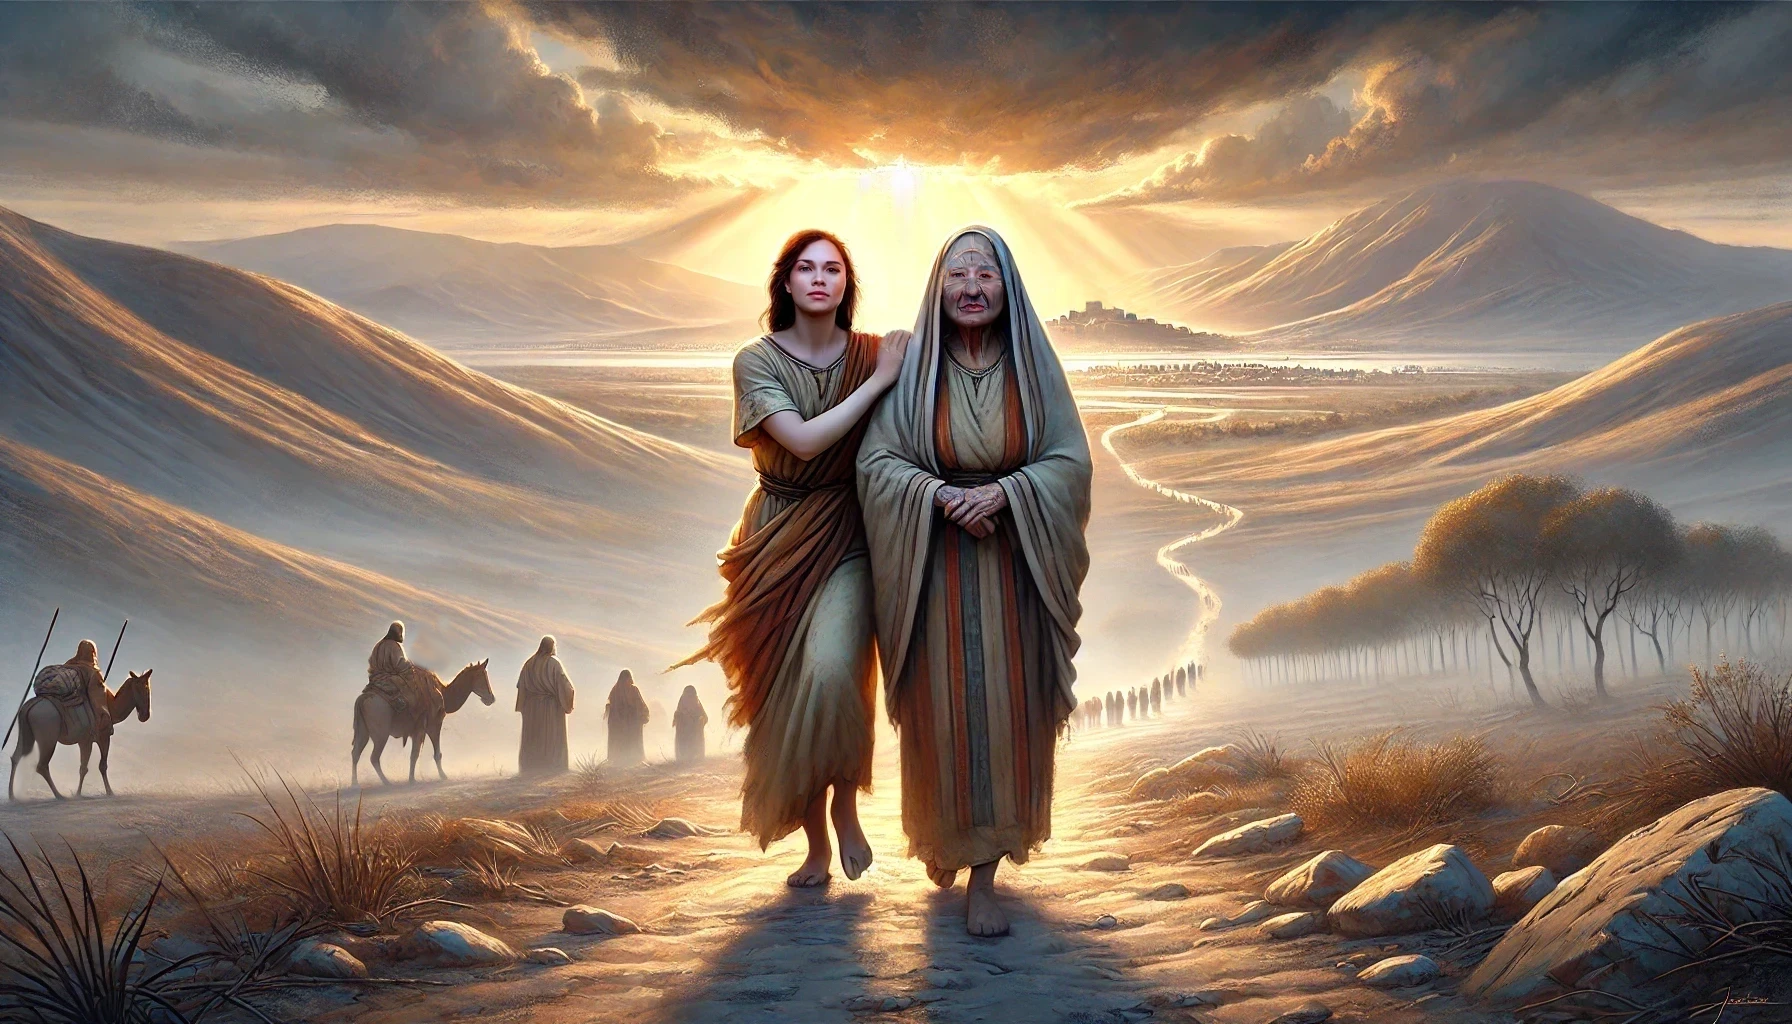
\includegraphics[width=0.7\linewidth]{graficas/Rut}\\
	Rut y Noemí  \\
	\end{center}



\section*{Capítulo 1}

Rut y Noemí  
1:1 Aconteció en los días que gobernaban los jueces, que hubo hambre en la tierra. Y un varón de Belén de Judá fue a morar en los campos de Moab, él y su mujer, y dos hijos suyos.  
1:2 El nombre de aquel varón era Elimelec, y el de su mujer, Noemí; y los nombres de sus hijos eran Mahlón y Quelión, efrateos de Belén de Judá. Llegaron, pues, a los campos de Moab, y se quedaron allí.  
1:3 Y murió Elimelec, marido de Noemí, y quedó ella con sus dos hijos,  
1:4 los cuales tomaron para sí mujeres moabitas; el nombre de una era Orfa, y el nombre de la otra, Rut; y habitaron allí unos diez años.  
1:5 Y murieron también los dos, Mahlón y Quelión, quedando así la mujer desamparada de sus dos hijos y de su marido.  
1:6 Entonces se levantó con sus nueras, y regresó de los campos de Moab; porque oyó en el campo de Moab que Jehová había visitado a su pueblo para darles pan.  
1:7 Salió, pues, del lugar donde había estado, y con ella sus dos nueras, y comenzaron a caminar para volverse a la tierra de Judá.  
1:8 Y Noemí dijo a sus dos nueras: Andad, volveos cada una a la casa de su madre; Jehová haga con vosotras misericordia, como la habéis hecho con los muertos y conmigo.  
1:9 Os conceda Jehová que halléis descanso, cada una en casa de su marido. Luego las besó, y ellas alzaron su voz y lloraron,  
1:10 y le dijeron: Ciertamente nosotras iremos contigo a tu pueblo.  
1:11 Y Noemí respondió: Volveos, hijas mías; ¿para qué habéis de ir conmigo? ¿Tengo yo más hijos en el vientre, que puedan ser vuestros maridos?  
1:12 Volveos, hijas mías, e idos; porque yo ya soy vieja para tener marido. Y aunque dijese: Esperanza tengo, y esta noche estuviese con marido, y aun diese a luz hijos,  
1:13 ¿habíais vosotras de esperarlos hasta que fuesen grandes? ¿Habíais de quedaros sin casar por amor a ellos? No, hijas mías; que mayor amargura tengo yo que vosotras, pues la mano de Jehová ha salido contra mí.  
1:14 Y ellas alzaron otra vez su voz y lloraron; y Orfa besó a su suegra, mas Rut se quedó con ella.  
1:15 Y Noemí dijo: He aquí tu cuñada se ha vuelto a su pueblo y a sus dioses; vuélvete tú tras ella.  
1:16 Respondió Rut: No me ruegues que te deje, y me aparte de ti; porque a dondequiera que tú fueres, iré yo, y dondequiera que vivieres, viviré. Tu pueblo será mi pueblo, y tu Dios mi Dios.  
1:17 Donde tú murieres, moriré yo, y allí seré sepultada; así me haga Jehová, y aun me añada, que sólo la muerte hará separación entre nosotras dos. 
1:18 Y viendo Noemí que estaba tan resuelta a ir con ella, no dijo más.  
1:19 Anduvieron, pues, ellas dos hasta que llegaron a Belén; y aconteció que habiendo entrado en Belén, toda la ciudad se conmovió por causa de ellas, y decían: ¿No es ésta Noemí?  
1:20 Y ella les respondía: No me llaméis Noemí, sino llamadme Mara; porque en grande amargura me ha puesto el Todopoderoso.  
1:21 Yo me fui llena, pero Jehová me ha vuelto con las manos vacías. ¿Por qué me llamaréis Noemí, ya que Jehová ha dado testimonio contra mí, y el Todopoderoso me ha afligido?  
1:22 Así volvió Noemí, y Rut la moabita su nuera con ella; volvió de los campos de Moab, y llegaron a Belén al comienzo de la siega de la cebada.  
\section*{Capítulo 2}
Rut recoge espigas en el campo de Booz  

2:1 Tenía Noemí un pariente de su marido, hombre rico de la familia de Elimelec, el cual se llamaba Booz.  
2:2 Y Rut la moabita dijo a Noemí: Te ruego que me dejes ir al campo, y recogeré espigas en pos de aquel a cuyos ojos hallare gracia. Y ella le respondió: Vé, hija mía.  
2:3 Fue, pues, y llegando, espigó en el campo en pos de los segadores; y aconteció que aquella parte del campo era de Booz, el cual era de la familia de Elimelec.  
2:4 Y he aquí que Booz vino de Belén, y dijo a los segadores: Jehová sea con vosotros. Y ellos respondieron: Jehová te bendiga.  
2:5 Y Booz dijo a su criado el mayordomo de los segadores: ¿De quién es esta joven?  
2:6 Y el criado, mayordomo de los segadores, respondió y dijo: Es la joven moabita que volvió con Noemí de los campos de Moab;  
2:7 y ha dicho: Te ruego que me dejes recoger y juntar tras los segadores entre las gavillas. Entró, pues, y está desde por la mañana hasta ahora, sin descansar ni aun por un momento.  
2:8 Entonces Booz dijo a Rut: Oye, hija mía, no vayas a espigar a otro campo, ni pases de aquí; y aquí estarás junto a mis criadas.  
2:9 Mira bien el campo que sieguen, y síguelas; porque yo he mandado a los criados que no te molesten. Y cuando tengas sed, ve a las vasijas, y bebe del agua que sacan los criados.  
2:10 Ella entonces bajando su rostro se inclinó a tierra, y le dijo: ¿Por qué he hallado gracia en tus ojos para que me reconozcas, siendo yo extranjera?  
2:11 Y respondiendo Booz, le dijo: He sabido todo lo que has hecho con tu suegra después de la muerte de tu marido, y que dejando a tu padre y a tu madre y la tierra donde naciste, has venido a un pueblo que no conociste antes.  
2:12 Jehová recompense tu obra, y tu remuneración sea cumplida de parte de Jehová Dios de Israel, bajo cuyas alas has venido a refugiarte.  
2:13 Y ella dijo: Señor mío, halle yo gracia delante de tus ojos; porque me has consolado, y porque has hablado al corazón de tu sierva, aunque no soy ni como una de tus criadas.  
2:14 Y Booz le dijo a la hora de comer: Ven aquí, y come del pan, y moja tu bocado en el vinagre. Y ella se sentó junto a los segadores, y él le dio del potaje, y comió hasta que se sació, y le sobró.  
2:15 Luego se levantó para espigar. Y Booz mandó a sus criados, diciendo: Que recoja también espigas entre las gavillas, y no la avergoncéis;  
2:16 y dejaréis también caer para ella algo de los manojos, y lo dejaréis para que lo recoja, y no la reprendáis.  
2:17 Espigó, pues, en el campo hasta la noche, y desgranó lo que había recogido, y fue como un efa  de cebada.  
2:18 Y lo tomó, y se fue a la ciudad; y su suegra vio lo que había recogido. Sacó también luego lo que le había sobrado después de haber quedado saciada, y se lo dio.  
2:19 Y le dijo su suegra: ¿Dónde has espigado hoy? ¿y dónde has trabajado? Bendito sea el que te ha reconocido. Y contó ella a su suegra con quién había trabajado, y dijo: El nombre del varón con quien hoy he trabajado es Booz.  
2:20 Y dijo Noemí a su nuera: Sea él bendito de Jehová, pues que no ha rehusado a los vivos la benevolencia que tuvo para con los que han muerto. Después le dijo Noemí: Nuestro pariente es aquel varón, y uno de los que pueden redimirnos.  
2:21 Y Rut la moabita dijo: Además de esto me ha dicho: Júntate con mis criadas, hasta que hayan acabado toda mi siega.  
2:22 Y Noemí respondió a Rut su nuera: Mejor es, hija mía, que salgas con sus criadas, y que no te encuentren en otro campo.  
2:23 Estuvo, pues, junto con las criadas de Booz espigando, hasta que se acabó la siega de la cebada y la del trigo; y vivía con su suegra.  
\section*{Capítulo 3}
Rut y Booz en la era  

3:1 Después le dijo su suegra Noemí: Hija mía, ¿no he de buscar hogar para ti, para que te vaya bien?  
3:2 ¿No es Booz nuestro pariente, con cuyas criadas tú has estado? He aquí que él avienta esta noche la parva de las cebadas.  
3:3 Te lavarás, pues, y te ungirás, y vistiéndote tus vestidos, irás a la era; mas no te darás a conocer al varón hasta que él haya acabado de comer y de beber.  
3:4 Y cuando él se acueste, notarás el lugar donde se acuesta, e irás y descubrirás sus pies, y te acostarás allí; y él te dirá lo que hayas de hacer.  
3:5 Y ella respondió: Haré todo lo que tú me mandes.  
3:6 Descendió, pues, a la era, e hizo todo lo que su suegra le había mandado.  
3:7 Y cuando Booz hubo comido y bebido, y su corazón estuvo contento, se retiró a dormir a un lado del montón. Entonces ella vino calladamente, y le descubrió los pies y se acostó.  
3:8 Y aconteció que a la medianoche se estremeció aquel hombre, y se volvió; y he aquí, una mujer estaba acostada a sus pies.  
3:9 Entonces él dijo: ¿Quién eres? Y ella respondió: Yo soy Rut tu sierva; extiende el borde de tu capa sobre tu sierva, por cuanto eres pariente cercano.  
3:10 Y él dijo: Bendita seas tú de Jehová, hija mía; has hecho mejor tu postrera bondad que la primera, no yendo en busca de los jóvenes, sean pobres o ricos.  
3:11 Ahora pues, no temas, hija mía; yo haré contigo lo que tú digas, pues toda la gente de mi pueblo sabe que eres mujer virtuosa.  
3:12 Y ahora, aunque es cierto que yo soy pariente cercano, con todo eso hay pariente más cercano que yo.  
3:13 Pasa aquí la noche, y cuando sea de día, si él te redimiere, bien, redímate; mas si él no te quisiere redimir, yo te redimiré, vive Jehová. Descansa, pues, hasta la mañana.  
3:14 Y después que durmió a sus pies hasta la mañana, se levantó antes que los hombres pudieran reconocerse unos a otros; porque él dijo: No se sepa que vino mujer a la era.  
3:15 Después le dijo: Quítate el manto que traes sobre ti, y tenlo. Y teniéndolo ella, él midió seis medidas  de cebada, y se las puso encima; y ella se fue a la ciudad.  
3:16 Y cuando llegó a donde estaba su suegra, ésta le dijo: ¿Qué hay, hija mía? Y le contó ella todo lo que con aquel varón le había acontecido.  
3:17 Y dijo: Estas seis medidas  de cebada me dio, diciéndome: A fin de que no vayas a tu suegra con las manos vacías.  
3:18 Entonces Noemí dijo: Espérate, hija mía, hasta que sepas cómo se resuelve el asunto; porque aquel hombre no descansará hasta que concluya el asunto hoy.  
\section*{Capítulo 4}
Booz se casa con Rut  

4:1 Booz subió a la puerta y se sentó allí; y he aquí pasaba aquel pariente de quien Booz había hablado, y le dijo: Eh, fulano, ven acá y siéntate. Y él vino y se sentó.  
4:2 Entonces él tomó a diez varones de los ancianos de la ciudad, y dijo: Sentaos aquí. Y ellos se sentaron.  
4:3 Luego dijo al pariente: Noemí, que ha vuelto del campo de Moab, vende una parte de las tierras que tuvo nuestro hermano Elimelec.  
4:4 Y yo decidí hacértelo saber, y decirte que la compres en presencia de los que están aquí sentados, y de los ancianos de mi pueblo. Si tú quieres redimir, redime; y si no quieres redimir, decláramelo para que yo lo sepa; porque no hay otro que redima sino tú, y yo después de ti. Y él respondió: Yo redimiré.  
4:5 Entonces replicó Booz: El mismo día que compres las tierras de mano de Noemí, debes tomar también a Rut la moabita, mujer del difunto, para que restaures el nombre del muerto sobre su posesión.  
4:6 Y respondió el pariente: No puedo redimir para mí, no sea que dañe mi heredad. Redime tú, usando de mi derecho, porque yo no podré redimir.  
4:7 Había ya desde hacía tiempo esta costumbre en Israel tocante a la redención y al contrato, que para la confirmación de cualquier negocio, el uno se quitaba el zapato y lo daba a su compañero; y esto servía de testimonio en Israel.  
4:8 Entonces el pariente dijo a Booz: Tómalo tú. Y se quitó el zapato. 
4:9 Y Booz dijo a los ancianos y a todo el pueblo: Vosotros sois testigos hoy, de que he adquirido de mano de Noemí todo lo que fue de Elimelec, y todo lo que fue de Quelión y de Mahlón.  
4:10 Y que también tomo por mi mujer a Rut la moabita, mujer de Mahlón, para restaurar el nombre del difunto sobre su heredad, para que el nombre del muerto no se borre de entre sus hermanos y de la puerta de su lugar. Vosotros sois testigos hoy.  
4:11 Y dijeron todos los del pueblo que estaban a la puerta con los ancianos: Testigos somos. Jehová haga a la mujer que entra en tu casa como a Raquel y a Lea, las cuales edificaron la casa de Israel; y tú seas ilustre en Efrata, y seas de renombre en Belén.  
4:12 Y sea tu casa como la casa de Fares, el que Tamar dio a luz a Judá, por la descendencia que de esa joven te dé Jehová.  
4:13 Booz, pues, tomó a Rut, y ella fue su mujer; y se llegó a ella, y Jehová le dio que concibiese y diese a luz un hijo.  
4:14 Y las mujeres decían a Noemí: Loado sea Jehová, que hizo que no te faltase hoy pariente, cuyo nombre será celebrado en Israel;  
4:15 el cual será restaurador de tu alma, y sustentará tu vejez; pues tu nuera, que te ama, lo ha dado a luz; y ella es de más valor para ti que siete hijos.  
4:16 Y tomando Noemí el hijo, lo puso en su regazo, y fue su aya.  
4:17 Y le dieron nombre las vecinas, diciendo: Le ha nacido un hijo a Noemí; y lo llamaron Obed. Este es padre de Isaí, padre de David.  
4:18 Estas son las generaciones de Fares: Fares engendró a Hezrón,  
4:19 Hezrón engendró a Ram, y Ram engendró a Aminadab,  
4:20 Aminadab engendró a Naasón, y Naasón engendró a Salmón,  
4:21 Salmón engendró a Booz, y Booz engendró a Obed,  
4:22 Obed engendró a Isaí, e Isaí engendró a David.

	
\chapter{Primer Libro de Samuel}

\section*{Capítulo 1 }
Nacimiento de Samuel  
1:1 Hubo un varón de Ramataim de Zofim, del monte de Efraín, que se llamaba Elcana hijo de Jeroham, hijo de Eliú, hijo de Tohu, hijo de Zuf, efrateo.  
1:2 Y tenía él dos mujeres; el nombre de una era Ana, y el de la otra, Penina. Y Penina tenía hijos, mas Ana no los tenía.  
1:3 Y todos los años aquel varón subía de su ciudad para adorar y para ofrecer sacrificios a Jehová de los ejércitos en Silo, donde estaban dos hijos de Elí, Ofni y Finees, sacerdotes de Jehová.  
1:4 Y cuando llegaba el día en que Elcana ofrecía sacrificio, daba a Penina su mujer, a todos sus hijos y a todas sus hijas, a cada uno su parte.  
1:5 Pero a Ana daba una parte escogida; porque amaba a Ana, aunque Jehová no le había concedido tener hijos.  
1:6 Y su rival la irritaba, enojándola y entristeciéndola, porque Jehová no le había concedido tener hijos.  
1:7 Así hacía cada año; cuando subía a la casa de Jehová, la irritaba así; por lo cual Ana lloraba, y no comía.  
1:8 Y Elcana su marido le dijo: Ana, ¿por qué lloras? ¿por qué no comes? ¿y por qué está afligido tu corazón? ¿No te soy yo mejor que diez hijos?  
1:9 Y se levantó Ana después que hubo comido y bebido en Silo; y mientras el sacerdote Elí estaba sentado en una silla junto a un pilar del templo de Jehová,  
1:10 ella con amargura de alma oró a Jehová, y lloró abundantemente.  
1:11 E hizo voto, diciendo: Jehová de los ejércitos, si te dignares mirar a la aflicción de tu sierva, y te acordares de mí, y no te olvidares de tu sierva, sino que dieres a tu sierva un hijo varón, yo lo dedicaré a Jehová todos los días de su vida, y no pasará navaja sobre su cabeza. 
1:12 Mientras ella oraba largamente delante de Jehová, Elí estaba observando la boca de ella.  
1:13 Pero Ana hablaba en su corazón, y solamente se movían sus labios, y su voz no se oía; y Elí la tuvo por ebria.  
1:14 Entonces le dijo Elí: ¿Hasta cuándo estarás ebria? Digiere tu vino.  
1:15 Y Ana le respondió diciendo: No, señor mío; yo soy una mujer atribulada de espíritu; no he bebido vino ni sidra, sino que he derramado mi alma delante de Jehová.  
1:16 No tengas a tu sierva por una mujer impía; porque por la magnitud de mis congojas y de mi aflicción he hablado hasta ahora.  
1:17 Elí respondió y dijo: Ve en paz, y el Dios de Israel te otorgue la petición que le has hecho.  
1:18 Y ella dijo: Halle tu sierva gracia delante de tus ojos. Y se fue la mujer por su camino, y comió, y no estuvo más triste.  
1:19 Y levantándose de mañana, adoraron delante de Jehová, y volvieron y fueron a su casa en Ramá. Y Elcana se llegó a Ana su mujer, y Jehová se acordó de ella.  
1:20 Aconteció que al cumplirse el tiempo, después de haber concebido Ana, dio a luz un hijo, y le puso por nombre Samuel, diciendo: Por cuanto lo pedí a Jehová.  
1:21 Después subió el varón Elcana con toda su familia, para ofrecer a Jehová el sacrificio acostumbrado y su voto.  
1:22 Pero Ana no subió, sino dijo a su marido: Yo no subiré hasta que el niño sea destetado, para que lo lleve y sea presentado delante de Jehová, y se quede allá para siempre.  
1:23 Y Elcana su marido le respondió: Haz lo que bien te parezca; quédate hasta que lo destetes; solamente que cumpla Jehová su palabra. Y se quedó la mujer, y crió a su hijo hasta que lo destetó.  
1:24 Después que lo hubo destetado, lo llevó consigo, con tres becerros, un efa  de harina, y una vasija de vino, y lo trajo a la casa de Jehová en Silo; y el niño era pequeño.  
1:25 Y matando el becerro, trajeron el niño a Elí.  
1:26 Y ella dijo: ¡Oh, señor mío! Vive tu alma, señor mío, yo soy aquella mujer que estuvo aquí junto a ti orando a Jehová.  
1:27 Por este niño oraba, y Jehová me dio lo que le pedí.  
1:28 Yo, pues, lo dedico también a Jehová; todos los días que viva, será de Jehová. Y adoró allí a Jehová.  

\section*{Capítulo 2}

Cántico de Ana  

2:1 Y Ana oró y dijo:  
Mi corazón se regocija en Jehová,  
Mi poder se exalta en Jehová;  
Mi boca se ensanchó sobre mis enemigos,  
Por cuanto me alegré en tu salvación.  
2:2 No hay santo como Jehová;  
Porque no hay ninguno fuera de ti,  
Y no hay refugio como el Dios nuestro.  
2:3 No multipliquéis palabras de grandeza y altanería; 
Cesen las palabras arrogantes de vuestra boca;  
Porque el Dios de todo saber es Jehová,  
Y a él toca el pesar las acciones. 
2:4 Los arcos de los fuertes fueron quebrados,  
Y los débiles se ciñeron de poder.  
2:5 Los saciados se alquilaron por pan,  
Y los hambrientos dejaron de tener hambre;  
Hasta la estéril ha dado a luz siete,  
Y la que tenía muchos hijos languidece.  
2:6 Jehová mata, y él da vida;  
El hace descender al Seol, y hace subir. 
2:7 Jehová empobrece, y él enriquece;  
Abate, y enaltece.  
2:8 El levanta del polvo al pobre,  
Y del muladar exalta al menesteroso,  
Para hacerle sentarse con príncipes y heredar un sitio de honor.  
Porque de Jehová son las columnas de la tierra,  
Y él afirmó sobre ellas el mundo.  
2:9 El guarda los pies de sus santos,  
Mas los impíos perecen en tinieblas;  
Porque nadie será fuerte por su propia fuerza.  
2:10 Delante de Jehová serán quebrantados sus adversarios,  
Y sobre ellos tronará desde los cielos;  
Jehová juzgará los confines de la tierra,  
Dará poder a su Rey,  
Y exaltará el poderío de su Ungido. 
2:11 Y Elcana se volvió a su casa en Ramá; y el niño ministraba a Jehová delante del sacerdote Elí.  
El pecado de los hijos de Elí  
2:12 Los hijos de Elí eran hombres impíos, y no tenían conocimiento de Jehová.  
2:13 Y era costumbre de los sacerdotes con el pueblo, que cuando alguno ofrecía sacrificio, venía el criado del sacerdote mientras se cocía la carne, trayendo en su mano un garfio de tres dientes,  
2:14 y lo metía en el perol, en la olla, en el caldero o en la marmita; y todo lo que sacaba el garfio, el sacerdote lo tomaba para sí. De esta manera hacían con todo israelita que venía a Silo.  
2:15 Asimismo, antes de quemar la grosura, venía el criado del sacerdote, y decía al que sacrificaba: Da carne que asar para el sacerdote; porque no tomará de ti carne cocida, sino cruda.  
2:16 Y si el hombre le respondía: Quemen la grosura primero, y después toma tanto como quieras; él respondía: No, sino dámela ahora mismo; de otra manera yo la tomaré por la fuerza.  
2:17 Era, pues, muy grande delante de Jehová el pecado de los jóvenes; porque los hombres menospreciaban las ofrendas de Jehová.  
2:18 Y el joven Samuel ministraba en la presencia de Jehová, vestido de un efod de lino.  
2:19 Y le hacía su madre una túnica pequeña y se la traía cada año, cuando subía con su marido para ofrecer el sacrificio acostumbrado.  
2:20 Y Elí bendijo a Elcana y a su mujer, diciendo: Jehová te dé hijos de esta mujer en lugar del que pidió a Jehová. Y se volvieron a su casa.  
2:21 Y visitó Jehová a Ana, y ella concibió, y dio a luz tres hijos y dos hijas. Y el joven Samuel crecía delante de Jehová.  
2:22 Pero Elí era muy viejo; y oía de todo lo que sus hijos hacían con todo Israel, y cómo dormían con las mujeres que velaban a la puerta del tabernáculo de reunión.  
2:23 Y les dijo: ¿Por qué hacéis cosas semejantes? Porque yo oigo de todo este pueblo vuestros malos procederes.  
2:24 No, hijos míos, porque no es buena fama la que yo oigo; pues hacéis pecar al pueblo de Jehová.  
2:25 Si pecare el hombre contra el hombre, los jueces le juzgarán; mas si alguno pecare contra Jehová, ¿quién rogará por él? Pero ellos no oyeron la voz de su padre, porque Jehová había resuelto hacerlos morir.  
2:26 Y el joven Samuel iba creciendo, y era acepto delante de Dios y delante de los hombres.  
2:27 Y vino un varón de Dios a Elí, y le dijo: Así ha dicho Jehová: ¿No me manifesté yo claramente a la casa de tu padre, cuando estaban en Egipto en casa de Faraón?  
2:28 Y yo le escogí por mi sacerdote entre todas las tribus de Israel, para que ofreciese sobre mi altar, y quemase incienso, y llevase efod delante de mí; y di a la casa de tu padre todas las ofrendas de los hijos de Israel. 
2:29 ¿Por qué habéis hollado mis sacrificios y mis ofrendas, que yo mandé ofrecer en el tabernáculo; y has honrado a tus hijos más que a mí, engordándoos de lo principal de todas las ofrendas de mi pueblo Israel?  
2:30 Por tanto, Jehová el Dios de Israel dice: Yo había dicho que tu casa y la casa de tu padre andarían delante de mí perpetuamente; mas ahora ha dicho Jehová: Nunca yo tal haga, porque yo honraré a los que me honran, y los que me desprecian serán tenidos en poco.  
2:31 He aquí, vienen días en que cortaré tu brazo y el brazo de la casa de tu padre, de modo que no haya anciano en tu casa.  
2:32 Verás tu casa humillada, mientras Dios colma de bienes a Israel; y en ningún tiempo habrá anciano en tu casa.  
2:33 El varón de los tuyos que yo no corte de mi altar, será para consumir tus ojos y llenar tu alma de dolor; y todos los nacidos en tu casa morirán en la edad viril.  
2:34 Y te será por señal esto que acontecerá a tus dos hijos, Ofni y Finees: ambos morirán en un día.  
2:35 Y yo me suscitaré un sacerdote fiel, que haga conforme a mi corazón y a mi alma; y yo le edificaré casa firme, y andará delante de mi ungido todos los días.  
2:36 Y el que hubiere quedado en tu casa vendrá a postrarse delante de él por una moneda de plata y un bocado de pan, diciéndole: Te ruego que me agregues a alguno de los ministerios, para que pueda comer un bocado de pan.  
\section*{Capítulo 3}
Jehová llama a Samuel  

3:1 El joven Samuel ministraba a Jehová en presencia de Elí; y la palabra de Jehová escaseaba en aquellos días; no había visión con frecuencia.  
3:2 Y aconteció un día, que estando Elí acostado en su aposento, cuando sus ojos comenzaban a oscurecerse de modo que no podía ver,  
3:3 Samuel estaba durmiendo en el templo de Jehová, donde estaba el arca de Dios; y antes que la lámpara de Dios fuese apagada,  
3:4 Jehová llamó a Samuel; y él respondió: Heme aquí.  
3:5 Y corriendo luego a Elí, dijo: Heme aquí, ¿Para qué me llamaste? Y Elí le dijo: Yo no he llamado; vuelve y acuéstate. Y él se volvió y se acostó.  
3:6 Y Jehová volvió a llamar otra vez a Samuel. Y levantándose Samuel, vino a Elí y dijo: Heme aquí; ¿para qué me has llamado? Y él dijo: Hijo mío, yo no he llamado; vuelve y acuéstate.  
3:7 Y Samuel no había conocido aún a Jehová, ni la palabra de Jehová le había sido revelada.  
3:8 Jehová, pues, llamó la tercera vez a Samuel. Y él se levantó y vino a Elí, y dijo: Heme aquí; ¿para qué me has llamado? Entonces entendió Elí que Jehová llamaba al joven.  
3:9 Y dijo Elí a Samuel: Ve y acuéstate; y si te llamare, dirás: Habla, Jehová, porque tu siervo oye. Así se fue Samuel, y se acostó en su lugar.  
3:10 Y vino Jehová y se paró, y llamó como las otras veces: ¡Samuel, Samuel! Entonces Samuel dijo: Habla, porque tu siervo oye.  
3:11 Y Jehová dijo a Samuel: He aquí haré yo una cosa en Israel, que a quien la oyere, le retiñirán ambos oídos.  
3:12 Aquel día yo cumpliré contra Elí todas las cosas que he dicho sobre su casa, desde el principio hasta el fin.  
3:13 Y le mostraré que yo juzgaré su casa para siempre, por la iniquidad que él sabe; porque sus hijos han blasfemado a Dios, y él no los ha estorbado.  
3:14 Por tanto, yo he jurado a la casa de Elí que la iniquidad de la casa de Elí no será expiada jamás, ni con sacrificios ni con ofrendas.  
3:15 Y Samuel estuvo acostado hasta la mañana, y abrió las puertas de la casa de Jehová. Y Samuel temía descubrir la visión a Elí.  
3:16 Llamando, pues, Elí a Samuel, le dijo: Hijo mío, Samuel. Y él respondió: Heme aquí.  
3:17 Y Elí dijo: ¿Qué es la palabra que te habló? Te ruego que no me la encubras; así te haga Dios y aun te añada, si me encubrieres palabra de todo lo que habló contigo.  
3:18 Y Samuel se lo manifestó todo, sin encubrirle nada. Entonces él dijo: Jehová es; haga lo que bien le pareciere.  
3:19 Y Samuel creció, y Jehová estaba con él, y no dejó caer a tierra ninguna de sus palabras.  
3:20 Y todo Israel, desde Dan hasta Beerseba, conoció que Samuel era fiel profeta de Jehová.  
3:21 Y Jehová volvió a aparecer en Silo; porque Jehová se manifestó a Samuel en Silo por la palabra de Jehová.  
\section*{Capítulo 4}
Los filisteos capturan el arca  

4:1 Y Samuel habló a todo Israel. Por aquel tiempo salió Israel a encontrar en batalla a los filisteos, y acampó junto a Eben- ezer, y los filisteos acamparon en Afec.  
4:2 Y los filisteos presentaron la batalla a Israel; y trabándose el combate, Israel fue vencido delante de los filisteos, los cuales hirieron en la batalla en el campo como a cuatro mil hombres.  
4:3 Cuando volvió el pueblo al campamento, los ancianos de Israel dijeron: ¿Por qué nos ha herido hoy Jehová delante de los filisteos? Traigamos a nosotros de Silo el arca del pacto de Jehová, para que viniendo entre nosotros nos salve de la mano de nuestros enemigos.  
4:4 Y envió el pueblo a Silo, y trajeron de allá el arca del pacto de Jehová de los ejércitos, que moraba entre los querubines; y los dos hijos de Elí, Ofni y Finees, estaban allí con el arca del pacto de Dios. 
4:5 Aconteció que cuando el arca del pacto de Jehová llegó al campamento, todo Israel gritó con tan gran júbilo que la tierra tembló.  
4:6 Cuando los filisteos oyeron la voz de júbilo, dijeron: ¿Qué voz de gran júbilo es esta en el campamento de los hebreos? Y supieron que el arca de Jehová había sido traída al campamento.  
4:7 Y los filisteos tuvieron miedo, porque decían: Ha venido Dios al campamento. Y dijeron: ¡Ay de nosotros! pues antes de ahora no fue así.  
4:8 ¡Ay de nosotros! ¿Quién nos librará de la mano de estos dioses poderosos? Estos son los dioses que hirieron a Egipto con toda plaga en el desierto.  
4:9 Esforzaos, oh filisteos, y sed hombres, para que no sirváis a los hebreos, como ellos os han servido a vosotros; sed hombres, y pelead.  
4:10 Pelearon, pues, los filisteos, e Israel fue vencido, y huyeron cada cual a sus tiendas; y fue hecha muy grande mortandad, pues cayeron de Israel treinta mil hombres de a pie.  
4:11 Y el arca de Dios fue tomada, y muertos los dos hijos de Elí, Ofni y Finees.  
4:12 Y corriendo de la batalla un hombre de Benjamín, llegó el mismo día a Silo, rotos sus vestidos y tierra sobre su cabeza;  
4:13 y cuando llegó, he aquí que Elí estaba sentado en una silla vigilando junto al camino, porque su corazón estaba temblando por causa del arca de Dios. Llegado, pues, aquel hombre a la ciudad, y dadas las nuevas, toda la ciudad gritó.  
4:14 Cuando Elí oyó el estruendo de la gritería, dijo: ¿Qué estruendo de alboroto es este? Y aquel hombre vino aprisa y dio las nuevas a Elí.  
4:15 Era ya Elí de edad de noventa y ocho años, y sus ojos se habían oscurecido, de modo que no podía ver.  
4:16 Dijo, pues, aquel hombre a Elí: Yo vengo de la batalla, he escapado hoy del combate. Y Elí dijo: ¿Qué ha acontecido, hijo mío?  
4:17 Y el mensajero respondió diciendo: Israel huyó delante de los filisteos, y también fue hecha gran mortandad en el pueblo; y también tus dos hijos, Ofni y Finees, fueron muertos, y el arca de Dios ha sido tomada. 
4:18 Y aconteció que cuando él hizo mención del arca de Dios, Elí cayó hacia atrás de la silla al lado de la puerta, y se desnucó y murió; porque era hombre viejo y pesado. Y había juzgado a Israel cuarenta años.  
4:19 Y su nuera la mujer de Finees, que estaba encinta, cercana al alumbramiento, oyendo el rumor que el arca de Dios había sido tomada, y muertos su suegro y su marido, se inclinó y dio a luz; porque le sobrevinieron sus dolores de repente.  
4:20 Y al tiempo que moría, le decían las que estaban junto a ella: No tengas temor, porque has dado a luz un hijo. Mas ella no respondió, ni se dio por entendida.  
4:21 Y llamó al niño Icabod, diciendo: ¡Traspasada es la gloria de Israel! por haber sido tomada el arca de Dios, y por la muerte de su suegro y de su marido.  
4:22 Dijo, pues: Traspasada es la gloria de Israel; porque ha sido tomada el arca de Dios.  
\section*{Capítulo 5}
El arca en tierra de los filisteoss  

5:1 Cuando los filisteos capturaron el arca de Dios, la llevaron desde Eben-ezer a Asdod.  
5:2 Y tomaron los filisteos el arca de Dios, y la metieron en la casa de Dagón, y la pusieron junto a Dagón.  
5:3 Y cuando al siguiente día los de Asdod se levantaron de mañana, he aquí Dagón postrado en tierra delante del arca de Jehová; y tomaron a Dagón y lo volvieron a su lugar.  
5:4 Y volviéndose a levantar de mañana el siguiente día, he aquí que Dagón había caído postrado en tierra delante del arca de Jehová; y la cabeza de Dagón y las dos palmas de sus manos estaban cortadas sobre el umbral, habiéndole quedado a Dagón el tronco solamente.  
5:5 Por esta causa los sacerdotes de Dagón y todos los que entran en el templo de Dagón no pisan el umbral de Dagón en Asdod, hasta hoy.  
5:6 Y se agravó la mano de Jehová sobre los de Asdod, y los destruyó y los hirió con tumores en Asdod y en todo su territorio.  
5:7 Y viendo esto los de Asdod, dijeron: No quede con nosotros el arca del Dios de Israel, porque su mano es dura sobre nosotros y sobre nuestro dios Dagón.  
5:8 Convocaron, pues, a todos los príncipes de los filisteos, y les dijeron: ¿Qué haremos del arca del Dios de Israel? Y ellos respondieron: Pásese el arca del Dios de Israel a Gat. Y pasaron allá el arca del Dios de Israel.  
5:9 Y aconteció que cuando la habían pasado, la mano de Jehová estuvo contra la ciudad con gran quebrantamiento, y afligió a los hombres de aquella ciudad desde el chico hasta el grande, y se llenaron de tumores.  
5:10 Entonces enviaron el arca de Dios a Ecrón. Y cuando el arca de Dios vino a Ecrón, los ecronitas dieron voces, diciendo: Han pasado a nosotros el arca del Dios de Israel para matarnos a nosotros y a nuestro pueblo.  
5:11 Y enviaron y reunieron a todos los príncipes de los filisteos, diciendo: Enviad el arca del Dios de Israel, y vuélvase a su lugar, y no nos mate a nosotros ni a nuestro pueblo; porque había consternación de muerte en toda la ciudad, y la mano de Dios se había agravado allí.  
5:12 Y los que no morían, eran heridos de tumores; y el clamor de la ciudad subía al cielo.  
\section*{Capítulo 6}
Los filisteos devuelven el arca  

6:1 Estuvo el arca de Jehová en la tierra de los filisteos siete meses.  
6:2 Entonces los filisteos, llamando a los sacerdotes y adivinos, preguntaron: ¿Qué haremos del arca de Jehová? Hacednos saber de qué manera la hemos de volver a enviar a su lugar.  
6:3 Ellos dijeron: Si enviáis el arca del Dios de Israel, no la enviéis vacía, sino pagadle la expiación; entonces seréis sanos, y conoceréis por qué no se apartó de vosotros su mano.  
6:4 Y ellos dijeron: ¿Y qué será la expiación que le pagaremos? Ellos respondieron: Conforme al número de los príncipes de los filisteos, cinco tumores de oro, y cinco ratones de oro, porque una misma plaga ha afligido a todos vosotros y a vuestros príncipes.  
6:5 Haréis, pues, figuras de vuestros tumores, y de vuestros ratones que destruyen la tierra, y daréis gloria al Dios de Israel; quizá aliviará su mano de sobre vosotros y de sobre vuestros dioses, y de sobre vuestra tierra.  
6:6 ¿Por qué endurecéis vuestro corazón, como los egipcios y Faraón endurecieron su corazón? Después que los había tratado así, ¿no los dejaron ir, y se fueron?  
6:7 Haced, pues, ahora un carro nuevo, y tomad luego dos vacas que críen, a las cuales no haya sido puesto yugo, y uncid las vacas al carro, y haced volver sus becerros de detrás de ellas a casa.  
6:8 Tomaréis luego el arca de Jehová, y la pondréis sobre el carro, y las joyas de oro que le habéis de pagar en ofrenda por la culpa, las pondréis en una caja al lado de ella; y la dejaréis que se vaya.  
6:9 Y observaréis; si sube por el camino de su tierra a Bet-semes, él nos ha hecho este mal tan grande; y si no, sabremos que no es su mano la que nos ha herido, sino que esto ocurrió por accidente.  
6:10 Y aquellos hombres lo hicieron así; tomando dos vacas que criaban, las uncieron al carro, y encerraron en casa sus becerros.  
6:11 Luego pusieron el arca de Jehová sobre el carro, y la caja con los ratones de oro y las figuras de sus tumores.  
6:12 Y las vacas se encaminaron por el camino de Bet-semes, y seguían camino recto, andando y bramando, sin apartarse ni a derecha ni a izquierda; y los príncipes de los filisteos fueron tras ellas hasta el límite de Bet-semes.  
6:13 Y los de Bet-semes segaban el trigo en el valle; y alzando los ojos vieron el arca, y se regocijaron cuando la vieron.  
6:14 Y el carro vino al campo de Josué de Bet-semes, y paró allí donde había una gran piedra; y ellos cortaron la madera del carro, y ofrecieron las vacas en holocausto a Jehová.  
6:15 Y los levitas bajaron el arca de Jehová, y la caja que estaba junto a ella, en la cual estaban las joyas de oro, y las pusieron sobre aquella gran piedra; y los hombres de Bet-semes sacrificaron holocaustos y dedicaron sacrificios a Jehová en aquel día.  
6:16 Cuando vieron esto los cinco príncipes de los filisteos, volvieron a Ecrón el mismo día.  
6:17 Estos fueron los tumores de oro que pagaron los filisteos en expiación a Jehová: por Asdod uno, por Gaza uno, por Ascalón uno, por Gat uno, por Ecrón uno.  
6:18 Y los ratones de oro fueron conforme al número de todas las ciudades de los filisteos pertenecientes a los cinco príncipes, así las ciudades fortificadas como las aldeas sin muro. La gran piedra sobre la cual pusieron el arca de Jehová está en el campo de Josué de Bet-semes hasta hoy.  
6:19 Entonces Dios hizo morir a los hombres de Bet-semes, porque habían mirado dentro del arca de Jehová; hizo morir del pueblo a cincuenta mil setenta hombres. Y lloró el pueblo, porque Jehová lo había herido con tan gran mortandad.  
6:20 Y dijeron los de Bet-semes: ¿Quién podrá estar delante de Jehová el Dios santo? ¿A quién subirá desde nosotros?  
6:21 Y enviaron mensajeros a los habitantes de Quiriat-jearim, diciendo: Los filisteos han devuelto el arca de Jehová; descended, pues, y llevadla a vosotros.  
\section*{Capítulo 7 }

7:1 Vinieron los de Quiriat-jearim y llevaron el arca de Jehová, y la pusieron en casa de Abinadab, situada en el collado; y santificaron a Eleazar su hijo para que guardase el arca de Jehová. 
7:2 Desde el día que llegó el arca a Quiriat-jearim pasaron muchos días, veinte años; y toda la casa de Israel lamentaba en pos de Jehová.  
Samuel, juez de Israel 
7:3 Habló Samuel a toda la casa de Israel, diciendo: Si de todo vuestro corazón os volvéis a Jehová, quitad los dioses ajenos y a Astarot de entre vosotros, y preparad vuestro corazón a Jehová, y sólo a él servid, y os librará de la mano de los filisteos.  
7:4 Entonces los hijos de Israel quitaron a los baales y a Astarot, y sirvieron sólo a Jehová.  
7:5 Y Samuel dijo: Reunid a todo Israel en Mizpa, y yo oraré por vosotros a Jehová.  
7:6 Y se reunieron en Mizpa, y sacaron agua, y la derramaron delante de Jehová, y ayunaron aquel día, y dijeron allí: Contra Jehová hemos pecado. Y juzgó Samuel a los hijos de Israel en Mizpa.  
7:7 Cuando oyeron los filisteos que los hijos de Israel estaban reunidos en Mizpa, subieron los príncipes de los filisteos contra Israel; y al oír esto los hijos de Israel, tuvieron temor de los filisteos.  
7:8 Entonces dijeron los hijos de Israel a Samuel: No ceses de clamar por nosotros a Jehová nuestro Dios, para que nos guarde de la mano de los filisteos.  
7:9 Y Samuel tomó un cordero de leche y lo sacrificó entero en holocausto a Jehová; y clamó Samuel a Jehová por Israel, y Jehová le oyó.  
7:10 Y aconteció que mientras Samuel sacrificaba el holocausto, los filisteos llegaron para pelear con los hijos de Israel. Mas Jehová tronó aquel día con gran estruendo sobre los filisteos, y los atemorizó, y fueron vencidos delante de Israel.  
7:11 Y saliendo los hijos de Israel de Mizpa, siguieron a los filisteos, hiriéndolos hasta abajo de Bet-car.  
7:12 Tomó luego Samuel una piedra y la puso entre Mizpa y Sen, y le puso por nombre Eben-ezer, diciendo: Hasta aquí nos ayudó Jehová. 
7:13 Así fueron sometidos los filisteos, y no volvieron más a entrar en el territorio de Israel; y la mano de Jehová estuvo contra los filisteos todos los días de Samuel.  
7:14 Y fueron restituidas a los hijos de Israel las ciudades que los filisteos habían tomado a los israelitas, desde Ecrón hasta Gat; e Israel libró su territorio de mano de los filisteos. Y hubo paz entre Israel y el amorreo.  
7:15 Y juzgó Samuel a Israel todo el tiempo que vivió.  
7:16 Y todos los años iba y daba vuelta a Bet-el, a Gilgal y a Mizpa, y juzgaba a Israel en todos estos lugares.  
7:17 Después volvía a Ramá, porque allí estaba su casa, y allí juzgaba a Israel; y edificó allí un altar a Jehová.  
\section*{Capítulo 8}
Israel pide rey  

8:1 Aconteció que habiendo Samuel envejecido, puso a sus hijos por jueces sobre Israel.  
8:2 Y el nombre de su hijo primogénito fue Joel, y el nombre del segundo, Abías; y eran jueces en Beerseba.  
8:3 Pero no anduvieron los hijos por los caminos de su padre, antes se volvieron tras la avaricia, dejándose sobornar y pervirtiendo el derecho.  
8:4 Entonces todos los ancianos de Israel se juntaron, y vinieron a Ramá para ver a Samuel,  
8:5 y le dijeron: He aquí tú has envejecido, y tus hijos no andan en tus caminos; por tanto, constitúyenos ahora un rey que nos juzgue, como tienen todas las naciones. 
8:6 Pero no agradó a Samuel esta palabra que dijeron: Danos un rey que nos juzgue. Y Samuel oró a Jehová.  
8:7 Y dijo Jehová a Samuel: Oye la voz del pueblo en todo lo que te digan; porque no te han desechado a ti, sino a mí me han desechado, para que no reine sobre ellos.  
8:8 Conforme a todas las obras que han hecho desde el día que los saqué de Egipto hasta hoy, dejándome a mí y sirviendo a dioses ajenos, así hacen también contigo.  
8:9 Ahora, pues, oye su voz; mas protesta solemnemente contra ellos, y muéstrales cómo les tratará el rey que reinará sobre ellos.  
8:10 Y refirió Samuel todas las palabras de Jehová al pueblo que le había pedido rey.  
8:11 Dijo, pues: Así hará el rey que reinará sobre vosotros: tomará vuestros hijos, y los pondrá en sus carros y en su gente de a caballo, para que corran delante de su carro;  
8:12 y nombrará para sí jefes de miles y jefes de cincuentenas; los pondrá asimismo a que aren sus campos y sieguen sus mieses, y a que hagan sus armas de guerra y los pertrechos de sus carros.  
8:13 Tomará también a vuestras hijas para que sean perfumadoras, cocineras y amasadoras.  
8:14 Asimismo tomará lo mejor de vuestras tierras, de vuestras viñas y de vuestros olivares, y los dará a sus siervos.  
8:15 Diezmará vuestro grano y vuestras viñas, para dar a sus oficiales y a sus siervos.  
8:16 Tomará vuestros siervos y vuestras siervas, vuestros mejores jóvenes, y vuestros asnos, y con ellos hará sus obras.  
8:17 Diezmará también vuestros rebaños, y seréis sus siervos.  
8:18 Y clamaréis aquel día a causa de vuestro rey que os habréis elegido, mas Jehová no os responderá en aquel día.  
8:19 Pero el pueblo no quiso oír la voz de Samuel, y dijo: No, sino que habrá rey sobre nosotros;  
8:20 y nosotros seremos también como todas las naciones, y nuestro rey nos gobernará, y saldrá delante de nosotros, y hará nuestras guerras.  
8:21 Y oyó Samuel todas las palabras del pueblo, y las refirió en oídos de Jehová.  
8:22 Y Jehová dijo a Samuel: Oye su voz, y pon rey sobre ellos. Entonces dijo Samuel a los varones de Israel: Idos cada uno a vuestra ciudad.  
\section*{Capítulo 9}
Saúl es elegido rey  

9:1 Había un varón de Benjamín, hombre valeroso, el cual se llamaba Cis, hijo de Abiel, hijo de Zeror, hijo de Becorat, hijo de Afía, hijo de un benjamita.  
9:2 Y tenía él un hijo que se llamaba Saúl, joven y hermoso. Entre los hijos de Israel no había otro más hermoso que él; de hombros arriba sobrepasaba a cualquiera del pueblo.  
9:3 Y se habían perdido las asnas de Cis, padre de Saúl; por lo que dijo Cis a Saúl su hijo: Toma ahora contigo alguno de los criados, y levántate, y ve a buscar las asnas.  
9:4 Y él pasó el monte de Efraín, y de allí a la tierra de Salisa, y no las hallaron. Pasaron luego por la tierra de Saalim, y tampoco. Después pasaron por la tierra de Benjamín, y no las encontraron.  
9:5 Cuando vinieron a la tierra de Zuf, Saúl dijo a su criado que tenía consigo: Ven, volvámonos; porque quizá mi padre, abandonada la preocupación por las asnas, estará acongojado por nosotros.  
9:6 El le respondió: He aquí ahora hay en esta ciudad un varón de Dios, que es hombre insigne; todo lo que él dice acontece sin falta. Vamos, pues, allá; quizá nos dará algún indicio acerca del objeto por el cual emprendimos nuestro camino.  
9:7 Respondió Saúl a su criado: Vamos ahora; pero ¿qué llevaremos al varón? Porque el pan de nuestras alforjas se ha acabado, y no tenemos qué ofrecerle al varón de Dios. ¿Qué tenemos?  
9:8 Entonces volvió el criado a responder a Saúl, diciendo: He aquí se halla en mi mano la cuarta parte de un siclo de plata; esto daré al varón de Dios, para que nos declare nuestro camino.  
9:9 (Antiguamente en Israel cualquiera que iba a consultar a Dios, decía así: Venid y vamos al vidente; porque al que hoy se llama profeta, entonces se le llamaba vidente.)  
9:10 Dijo entonces Saúl a su criado: Dices bien; anda, vamos. Y fueron a la ciudad donde estaba el varón de Dios.  
9:11 Y cuando subían por la cuesta de la ciudad, hallaron unas doncellas que salían por agua, a las cuales dijeron: ¿Está en este lugar el vidente?  
9:12 Ellas, respondiéndoles, dijeron: Sí; helo allí delante de ti; date prisa, pues, porque hoy ha venido a la ciudad en atención a que el pueblo tiene hoy un sacrificio en el lugar alto.  
9:13 Cuando entréis en la ciudad, le encontraréis luego, antes que suba al lugar alto a comer; pues el pueblo no comerá hasta que él haya llegado, por cuanto él es el que bendice el sacrificio; después de esto comen los convidados. Subid, pues, ahora, porque ahora le hallaréis.  
9:14 Ellos entonces subieron a la ciudad; y cuando estuvieron en medio de ella, he aquí Samuel venía hacía ellos para subir al lugar alto.  
9:15 Y un día antes que Saúl viniese, Jehová había revelado al oído de Samuel, diciendo:  
9:16 Mañana a esta misma hora yo enviaré a ti un varón de la tierra de Benjamín, al cual ungirás por príncipe sobre mi pueblo Israel, y salvará a mi pueblo de mano de los filisteos; porque yo he mirado a mi pueblo, por cuanto su clamor ha llegado hasta mí.  
9:17 Y luego que Samuel vio a Saúl, Jehová le dijo: He aquí éste es el varón del cual te hablé; éste gobernará a mi pueblo.  
9:18 Acercándose, pues, Saúl a Samuel en medio de la puerta, le dijo: Te ruego que me enseñes dónde está la casa del vidente.  
9:19 Y Samuel respondió a Saúl, diciendo: Yo soy el vidente; sube delante de mí al lugar alto, y come hoy conmigo, y por la mañana te despacharé, y te descubriré todo lo que está en tu corazón.  
9:20 Y de las asnas que se te perdieron hace ya tres días, pierde cuidado de ellas, porque se han hallado. Mas ¿para quién es todo lo que hay de codiciable en Israel, sino para ti y para toda la casa de tu padre?  
9:21 Saúl respondió y dijo: ¿No soy yo hijo de Benjamín, de la más pequeña de las tribus de Israel? Y mi familia ¿no es la más pequeña de todas las familias de la tribu de Benjamín? ¿Por qué, pues, me has dicho cosa semejante?  
9:22 Entonces Samuel tomó a Saúl y a su criado, los introdujo a la sala, y les dio lugar a la cabecera de los convidados, que eran unos treinta hombres.  
9:23 Y dijo Samuel al cocinero: Trae acá la porción que te di, la cual te dije que guardases aparte.  
9:24 Entonces alzó el cocinero una espaldilla, con lo que estaba sobre ella, y la puso delante de Saúl. Y Samuel dijo: He aquí lo que estaba reservado; ponlo delante de ti y come, porque para esta ocasión se te guardó, cuando dije: Yo he convidado al pueblo. Y Saúl comió aquel día con Samuel.  
9:25 Y cuando hubieron descendido del lugar alto a la ciudad, él habló con Saúl en el terrado.  
9:26 Al otro día madrugaron; y al despuntar el alba, Samuel llamó a Saúl, que estaba en el terrado, y dijo: Levántate, para que te despida. Luego se levantó Saúl, y salieron ambos, él y Samuel.  
9:27 Y descendiendo ellos al extremo de la ciudad, dijo Samuel a Saúl: Di al criado que se adelante (y se adelantó el criado), mas espera tú un poco para que te declare la palabra de Dios.  
\section*{Capítulo 10 }

10:1 Tomando entonces Samuel una redoma de aceite, la derramó sobre su cabeza, y lo besó, y le dijo: ¿No te ha ungido Jehová por príncipe sobre su pueblo Israel?  
10:2 Hoy, después que te hayas apartado de mí, hallarás dos hombres junto al sepulcro de Raquel, en el territorio de Benjamín, en Selsa, los cuales te dirán: Las asnas que habías ido a buscar se han hallado; tu padre ha dejado ya de inquietarse por las asnas, y está afligido por vosotros, diciendo: ¿Qué haré acerca de mi hijo?  
10:3 Y luego que de allí sigas más adelante, y llegues a la encina de Tabor, te saldrán al encuentro tres hombres que suben a Dios en Bet-el, llevando uno tres cabritos, otro tres tortas de pan, y el tercero una vasija de vino;  
10:4 los cuales, luego que te hayan saludado, te darán dos panes, los que tomarás de mano de ellos.  
10:5 Después de esto llegarás al collado de Dios donde está la guarnición de los filisteos; y cuando entres allá en la ciudad encontrarás una compañía de profetas que descienden del lugar alto, y delante de ellos salterio, pandero, flauta y arpa, y ellos profetizando.  
10:6 Entonces el Espíritu de Jehová vendrá sobre ti con poder, y profetizarás con ellos, y serás mudado en otro hombre.  
10:7 Y cuando te hayan sucedido estas señales, haz lo que te viniere a la mano, porque Dios está contigo.  
10:8 Luego bajarás delante de mí a Gilgal; entonces descenderé yo a ti para ofrecer holocaustos y sacrificar ofrendas de paz. Espera siete días, hasta que yo venga a ti y te enseñe lo que has de hacer.  
10:9 Aconteció luego, que al volver él la espalda para apartarse de Samuel, le mudó Dios su corazón; y todas estas señales acontecieron en aquel día.  
10:10 Y cuando llegaron allá al collado, he aquí la compañía de los profetas que venía a encontrarse con él; y el Espíritu de Dios vino sobre él con poder, y profetizó entre ellos.  
10:11 Y aconteció que cuando todos los que le conocían antes vieron que profetizaba con los profetas, el pueblo decía el uno al otro: ¿Qué le ha sucedido al hijo de Cis? ¿Saúl también entre los profetas?  
10:12 Y alguno de allí respondió diciendo: ¿Y quién es el padre de ellos? Por esta causa se hizo proverbio: ¿También Saúl entre los profetas?  
10:13 Y cesó de profetizar, y llegó al lugar alto.  
10:14 Un tío de Saúl dijo a él y a su criado: ¿A dónde fuisteis? Y él respondió: A buscar las asnas; y como vimos que no parecían, fuimos a Samuel.  
10:15 Dijo el tío de Saúl: Yo te ruego me declares qué os dijo Samuel.  
10:16 Y Saúl respondió a su tío: Nos declaró expresamente que las asnas habían sido halladas. Mas del asunto del reino, de que Samuel le había hablado, no le descubrió nada.  
10:17 Después Samuel convocó al pueblo delante de Jehová en Mizpa,  
10:18 y dijo a los hijos de Israel: Así ha dicho Jehová el Dios de Israel: Yo saqué a Israel de Egipto, y os libré de mano de los egipcios, y de mano de todos los reinos que os afligieron.  
10:19 Pero vosotros habéis desechado hoy a vuestro Dios, que os guarda de todas vuestras aflicciones y angustias, y habéis dicho: No, sino pon rey sobre nosotros. Ahora, pues, presentaos delante de Jehová por vuestras tribus y por vuestros millares.  
10:20 Y haciendo Samuel que se acercasen todas las tribus de Israel, fue tomada la tribu de Benjamín.  
10:21 E hizo llegar la tribu de Benjamín por sus familias, y fue tomada la familia de Matri; y de ella fue tomado Saúl hijo de Cis. Y le buscaron, pero no fue hallado.  
10:22 Preguntaron, pues, otra vez a Jehová si aún no había venido allí aquel varón. Y respondió Jehová: He aquí que él está escondido entre el bagaje.  
10:23 Entonces corrieron y lo trajeron de allí; y puesto en medio del pueblo, desde los hombros arriba era más alto que todo el pueblo.  
10:24 Y Samuel dijo a todo el pueblo: ¿Habéis visto al que ha elegido Jehová, que no hay semejante a él en todo el pueblo? Entonces el pueblo clamó con alegría, diciendo: ¡Viva el rey!  
10:25 Samuel recitó luego al pueblo las leyes del reino, y las escribió en un libro, el cual guardó delante de Jehová.  
10:26 Y envió Samuel a todo el pueblo cada uno a su casa. Saúl también se fue a su casa en Gabaa, y fueron con él los hombres de guerra cuyos corazones Dios había tocado.  
10:27 Pero algunos perversos dijeron: ¿Cómo nos ha de salvar éste? Y le tuvieron en poco, y no le trajeron presente; mas él disimuló.  
\section*{Capítulo 11 }
Saúl derrota a los amonitas  

11:1 Después subió Nahas amonita, y acampó contra Jabes de Galaad. Y todos los de Jabes dijeron a Nahas: Haz alianza con nosotros, y te serviremos.  
11:2 Y Nahas amonita les respondió: Con esta condición haré alianza con vosotros, que a cada uno de todos vosotros saque el ojo derecho, y ponga esta afrenta sobre todo Israel.  
11:3 Entonces los ancianos de Jabes le dijeron: Danos siete días, para que enviemos mensajeros por todo el territorio de Israel; y si no hay nadie que nos defienda, saldremos a ti.  
11:4 Llegando los mensajeros a Gabaa de Saúl, dijeron estas palabras en oídos del pueblo; y todo el pueblo alzó su voz y lloró.  
11:5 Y he aquí Saúl que venía del campo, tras los bueyes; y dijo Saúl: ¿Qué tiene el pueblo, que llora? Y le contaron las palabras de los hombres de Jabes.  
11:6 Al oír Saúl estas palabras, el Espíritu de Dios vino sobre él con poder; y él se encendió en ira en gran manera.  
11:7 Y tomando un par de bueyes, los cortó en trozos y los envió por todo el territorio de Israel por medio de mensajeros, diciendo: Así se hará con los bueyes del que no saliere en pos de Saúl y en pos de Samuel. Y cayó temor de Jehová sobre el pueblo, y salieron como un solo hombre.  
11:8 Y los contó en Bezec; y fueron los hijos de Israel trescientos mil, y treinta mil los hombres de Judá.  
11:9 Y respondieron a los mensajeros que habían venido: Así diréis a los de Jabes de Galaad: Mañana al calentar el sol, seréis librados. Y vinieron los mensajeros y lo anunciaron a los de Jabes, los cuales se alegraron.  
11:10 Y los de Jabes dijeron a los enemigos: Mañana saldremos a vosotros, para que hagáis con nosotros todo lo que bien os pareciere.  
11:11 Aconteció que al día siguiente dispuso Saúl al pueblo en tres compañías, y entraron en medio del campamento a la vigilia de la mañana, e hirieron a los amonitas hasta que el día calentó; y los que quedaron fueron dispersos, de tal manera que no quedaron dos de ellos juntos.  
11:12 El pueblo entonces dijo a Samuel: ¿Quiénes son los que decían: ¿Ha de reinar Saúl sobre nosotros? Dadnos esos hombres, y los mataremos.  
11:13 Y Saúl dijo: No morirá hoy ninguno, porque hoy Jehová ha dado salvación en Israel.  
11:14 Mas Samuel dijo al pueblo: Venid, vamos a Gilgal para que renovemos allí el reino.  
11:15 Y fue todo el pueblo a Gilgal, e invistieron allí a Saúl por rey delante de Jehová en Gilgal. Y sacrificaron allí ofrendas de paz delante de Jehová, y se alegraron mucho allí Saúl y todos los de Israel.  
\section*{Capítulo 12 }
Discurso de Samuel al pueblo  

12:1 Dijo Samuel a todo Israel: He aquí, yo he oído vuestra voz en todo cuanto me habéis dicho, y os he puesto rey.  
12:2 Ahora, pues, he aquí vuestro rey va delante de vosotros. Yo soy ya viejo y lleno de canas; pero mis hijos están con vosotros, y yo he andado delante de vosotros desde mi juventud hasta este día.  
12:3 Aquí estoy; atestiguad contra mí delante de Jehová y delante de su ungido, si he tomado el buey de alguno, si he tomado el asno de alguno, si he calumniado a alguien, si he agraviado a alguno, o si de alguien he tomado cohecho para cegar mis ojos con él; y os lo restituiré.  
12:4 Entonces dijeron: Nunca nos has calumniado ni agraviado, ni has tomado algo de mano de ningún hombre.  
12:5 Y él les dijo: Jehová es testigo contra vosotros, y su ungido también es testigo en este día, que no habéis hallado cosa alguna en mi mano. Y ellos respondieron: Así es.  
12:6 Entonces Samuel dijo al pueblo: Jehová que designó a Moisés y a Aarón, y sacó a vuestros padres de la tierra de Egipto, es testigo.  
12:7 Ahora, pues, aguardad, y contenderé con vosotros delante de Jehová acerca de todos los hechos de salvación que Jehová ha hecho con vosotros y con vuestros padres.  
12:8 Cuando Jacob hubo entrado en Egipto, y vuestros padres clamaron a Jehová, Jehová envió a Moisés y a Aarón, los cuales sacaron a vuestros padres de Egipto, y los hicieron habitar en este lugar.  
12:9 Y olvidaron a Jehová su Dios, y él los vendió en mano de Sísara jefe del ejército de Hazor, y en mano de los filisteos, y en mano del rey de Moab, los cuales les hicieron guerra.  
12:10 Y ellos clamaron a Jehová, y dijeron: Hemos pecado, porque hemos dejado a Jehová y hemos servido a los baales y a Astarot; líbranos, pues, ahora de mano de nuestros enemigos, y te serviremos. 
12:11 Entonces Jehová envió a Jerobaal, a Barac, a Jefté y a Samuel, y os libró de mano de vuestros enemigos en derredor, y habitasteis seguros.  
12:12 Y habiendo visto que Nahas rey de los hijos de Amón venía contra vosotros, me dijisteis: No, sino que ha de reinar sobre nosotros un rey; siendo así que Jehová vuestro Dios era vuestro rey.  
12:13 Ahora, pues, he aquí el rey que habéis elegido, el cual pedisteis; ya veis que Jehová ha puesto rey sobre vosotros.  
12:14 Si temiereis a Jehová y le sirviereis, y oyereis su voz, y no fuereis rebeldes a la palabra de Jehová, y si tanto vosotros como el rey que reina sobre vosotros servís a Jehová vuestro Dios, haréis bien.  
12:15 Mas si no oyereis la voz de Jehová, y si fuereis rebeldes a las palabras de Jehová, la mano de Jehová estará contra vosotros como estuvo contra vuestros padres.  
12:16 Esperad aún ahora, y mirad esta gran cosa que Jehová hará delante de vuestros ojos.  
12:17 ¿No es ahora la siega del trigo? Yo clamaré a Jehová, y él dará truenos y lluvias, para que conozcáis y veáis que es grande vuestra maldad que habéis hecho ante los ojos de Jehová, pidiendo para vosotros rey.  
12:18 Y Samuel clamó a Jehová, y Jehová dio truenos y lluvias en aquel día; y todo el pueblo tuvo gran temor de Jehová y de Samuel.  
12:19 Entonces dijo todo el pueblo a Samuel: Ruega por tus siervos a Jehová tu Dios, para que no muramos; porque a todos nuestros pecados hemos añadido este mal de pedir rey para nosotros.  
12:20 Y Samuel respondió al pueblo: No temáis; vosotros habéis hecho todo este mal; pero con todo eso no os apartéis de en pos de Jehová, sino servidle con todo vuestro corazón.  
12:21 No os apartéis en pos de vanidades que no aprovechan ni libran, porque son vanidades.  
12:22 Pues Jehová no desamparará a su pueblo, por su grande nombre; porque Jehová ha querido haceros pueblo suyo.  
12:23 Así que, lejos sea de mí que peque yo contra Jehová cesando de rogar por vosotros; antes os instruiré en el camino bueno y recto.  
12:24 Solamente temed a Jehová y servidle de verdad con todo vuestro corazón, pues considerad cuán grandes cosas ha hecho por vosotros.  
12:25 Mas si perseverareis en hacer mal, vosotros y vuestro rey pereceréis.  
\section*{Capítulo 13}
Guerra contra los filisteos  

13:1 Había ya reinado Saúl un año; y cuando hubo reinado dos años sobre Israel,  
13:2 escogió luego a tres mil hombres de Israel, de los cuales estaban con Saúl dos mil en Micmas y en el monte de Bet-el, y mil estaban con Jonatán en Gabaa de Benjamín; y envió al resto del pueblo cada uno a sus tiendas.  
13:3 Y Jonatán atacó a la guarnición de los filisteos que había en el collado, y lo oyeron los filisteos. E hizo Saúl tocar trompeta por todo el país, diciendo: Oigan los hebreos.  
13:4 Y todo Israel oyó que se decía: Saúl ha atacado a la guarnición de los filisteos; y también que Israel se había hecho abominable a los filisteos. Y se juntó el pueblo en pos de Saúl en Gilgal.  
13:5 Entonces los filisteos se juntaron para pelear contra Israel, treinta mil carros, seis mil hombres de a caballo, y pueblo numeroso como la arena que está a la orilla del mar; y subieron y acamparon en Micmas, al oriente de Bet-avén.  
13:6 Cuando los hombres de Israel vieron que estaban en estrecho (porque el pueblo estaba en aprieto), se escondieron en cuevas, en fosos, en peñascos, en rocas y en cisternas.  
13:7 Y algunos de los hebreos pasaron el Jordán a la tierra de Gad y de Galaad; pero Saúl permanecía aún en Gilgal, y todo el pueblo iba tras él temblando.  
13:8 Y él esperó siete días, conforme al plazo que Samuel había dicho; pero Samuel no venía a Gilgal, y el pueblo se le desertaba.  
13:9 Entonces dijo Saúl: Traedme holocausto y ofrendas de paz. Y ofreció el holocausto.  
13:10 Y cuando él acababa de ofrecer el holocausto, he aquí Samuel que venía; y Saúl salió a recibirle, para saludarle.  
13:11 Entonces Samuel dijo: ¿Qué has hecho? Y Saúl respondió: Porque vi que el pueblo se me desertaba, y que tú no venías dentro del plazo señalado, y que los filisteos estaban reunidos en Micmas,  
13:12 me dije: Ahora descenderán los filisteos contra mí a Gilgal, y yo no he implorado el favor de Jehová. Me esforcé, pues, y ofrecí holocausto.  
13:13 Entonces Samuel dijo a Saúl: Locamente has hecho; no guardaste el mandamiento de Jehová tu Dios que él te había ordenado; pues ahora Jehová hubiera confirmado tu reino sobre Israel para siempre.  
13:14 Mas ahora tu reino no será duradero. Jehová se ha buscado un varón conforme a su corazón, al cual Jehová ha designado para que sea príncipe sobre su pueblo, por cuanto tú no has guardado lo que Jehová te mandó.  
13:15 Y levantándose Samuel, subió de Gilgal a Gabaa de Benjamín. Y Saúl contó la gente que se hallaba con él, como seiscientos hombres.  
13:16 Saúl, pues, y Jonatán su hijo, y el pueblo que con ellos se hallaba, se quedaron en Gabaa de Benjamín; pero los filisteos habían acampado en Micmas.  
13:17 Y salieron merodeadores del campamento de los filisteos en tres escuadrones; un escuadrón marchaba por el camino de Ofra hacia la tierra de Sual,  
13:18 otro escuadrón marchaba hacia Bet-horón, y el tercer escuadrón marchaba hacia la región que mira al valle de Zeboim, hacia el desierto.  
13:19 Y en toda la tierra de Israel no se hallaba herrero; porque los filisteos habían dicho: Para que los hebreos no hagan espada o lanza.  
13:20 Por lo cual todos los de Israel tenían que descender a los filisteos para afilar cada uno la reja de su arado, su azadón, su hacha o su hoz.  
13:21 Y el precio era un pim por las rejas de arado y por los azadones, y la tercera parte de un siclo  por afilar las hachas y por componer las aguijadas.  
13:22 Así aconteció que en el día de la batalla no se halló espada ni lanza en mano de ninguno del pueblo que estaba con Saúl y con Jonatán, excepto Saúl y Jonatán su hijo, que las tenían.  
13:23 Y la guarnición de los filisteos avanzó hasta el paso de Micmas.  
\section*{Capítulo 14 }

14:1 Aconteció un día, que Jonatán hijo de Saúl dijo a su criado que le traía las armas: Ven y pasemos a la guarnición de los filisteos, que está de aquel lado. Y no lo hizo saber a su padre.  
14:2 Y Saúl se hallaba al extremo de Gabaa, debajo de un granado que hay en Migrón, y la gente que estaba con él era como seiscientos hombres.  
14:3 Y Ahías hijo de Ahitob, hermano de Icabod, hijo de Finees, hijo de Elí, sacerdote de Jehová en Silo, llevaba el efod; y no sabía el pueblo que Jonatán se hubiese ido.  
14:4 Y entre los desfiladeros por donde Jonatán procuraba pasar a la guarnición de los filisteos, había un peñasco agudo de un lado, y otro del otro lado; el uno se llamaba Boses, y el otro Sene.  
14:5 Uno de los peñascos estaba situado al norte, hacia Micmas, y el otro al sur, hacia Gabaa.  
14:6 Dijo, pues, Jonatán a su paje de armas: Ven, pasemos a la guarnición de estos incircuncisos; quizá haga algo Jehová por nosotros, pues no es difícil para Jehová salvar con muchos o con pocos.  
14:7 Y su paje de armas le respondió: Haz todo lo que tienes en tu corazón; ve, pues aquí estoy contigo a tu voluntad.  
14:8 Dijo entonces Jonatán: Vamos a pasar a esos hombres, y nos mostraremos a ellos.  
14:9 Si nos dijeren así: Esperad hasta que lleguemos a vosotros, entonces nos estaremos en nuestro lugar, y no subiremos a ellos.  
14:10 Mas si nos dijeren así: Subid a nosotros, entonces subiremos, porque Jehová los ha entregado en nuestra mano; y esto nos será por señal.  
14:11 Se mostraron, pues, ambos a la guarnición de los filisteos, y los filisteos dijeron: He aquí los hebreos, que salen de las cavernas donde se habían escondido.  
14:12 Y los hombres de la guarnición respondieron a Jonatán y a su paje de armas, y dijeron: Subid a nosotros, y os haremos saber una cosa. Entonces Jonatán dijo a su paje de armas: Sube tras mí, porque Jehová los ha entregado en manos de Israel.  
14:13 Y subió Jonatán trepando con sus manos y sus pies, y tras él su paje de armas; y a los que caían delante de Jonatán, su paje de armas que iba tras él los mataba.  
14:14 Y fue esta primera matanza que hicieron Jonatán y su paje de armas, como veinte hombres, en el espacio de una media yugada de tierra.  
14:15 Y hubo pánico en el campamento y por el campo, y entre toda la gente de la guarnición; y los que habían ido a merodear, también ellos tuvieron pánico, y la tierra tembló; hubo, pues, gran consternación.  
14:16 Y los centinelas de Saúl vieron desde Gabaa de Benjamín cómo la multitud estaba turbada, e iba de un lado a otro y era deshecha.  
14:17 Entonces Saúl dijo al pueblo que estaba con él: Pasad ahora revista, y ved quién se haya ido de los nuestros. Pasaron revista, y he aquí que faltaba Jonatán y su paje de armas.  
14:18 Y Saúl dijo a Ahías: Trae el arca de Dios. Porque el arca de Dios estaba entonces con los hijos de Israel.  
14:19 Pero aconteció que mientras aún hablaba Saúl con el sacerdote, el alboroto que había en el campamento de los filisteos aumentaba, e iba creciendo en gran manera. Entonces dijo Saúl al sacerdote: Detén tu mano.  
14:20 Y juntando Saúl a todo el pueblo que con él estaba, llegaron hasta el lugar de la batalla; y he aquí que la espada de cada uno estaba vuelta contra su compañero, y había gran confusión.  
14:21 Y los hebreos que habían estado con los filisteos de tiempo atrás, y habían venido con ellos de los alrededores al campamento, se pusieron también del lado de los israelitas que estaban con Saúl y con Jonatán.  
14:22 Asimismo todos los israelitas que se habían escondido en el monte de Efraín, oyendo que los filisteos huían, también ellos los persiguieron en aquella batalla.  
14:23 Así salvó Jehová a Israel aquel día. Y llegó la batalla hasta Bet-avén.  
14:24 Pero los hombres de Israel fueron puestos en apuro aquel día; porque Saúl había juramentado al pueblo, diciendo: Cualquiera que coma pan antes de caer la noche, antes que haya tomado venganza de mis enemigos, sea maldito. Y todo el pueblo no había probado pan.  
14:25 Y todo el pueblo llegó a un bosque, donde había miel en la superficie del campo.  
14:26 Entró, pues, el pueblo en el bosque, y he aquí que la miel corría; pero no hubo quien hiciera llegar su mano a su boca, porque el pueblo temía el juramento.  
14:27 Pero Jonatán no había oído cuando su padre había juramentado al pueblo, y alargó la punta de una vara que traía en su mano, y la mojó en un panal de miel, y llevó su mano a la boca; y fueron aclarados sus ojos.  
14:28 Entonces habló uno del pueblo, diciendo: Tu padre ha hecho jurar solemnemente al pueblo, diciendo: Maldito sea el hombre que tome hoy alimento. Y el pueblo desfallecía.  
14:29 Respondió Jonatán: Mi padre ha turbado el país. Ved ahora cómo han sido aclarados mis ojos, por haber gustado un poco de esta miel.  
14:30 ¿Cuánto más si el pueblo hubiera comido libremente hoy del botín tomado de sus enemigos? ¿No se habría hecho ahora mayor estrago entre los filisteos? 
14:31 E hirieron aquel día a los filisteos desde Micmas hasta Ajalón; pero el pueblo estaba muy cansado.  
14:32 Y se lanzó el pueblo sobre el botín, y tomaron ovejas y vacas y becerros, y los degollaron en el suelo; y el pueblo los comió con sangre.  
14:33 Y le dieron aviso a Saúl, diciendo: El pueblo peca contra Jehová, comiendo la carne con la sangre. Y él dijo: Vosotros habéis prevaricado; rodadme ahora acá una piedra grande.  
14:34 Además dijo Saúl: Esparcíos por el pueblo, y decidles que me traigan cada uno su vaca, y cada cual su oveja, y degolladlas aquí, y comed; y no pequéis contra Jehová comiendo la carne con la sangre. Y trajo todo el pueblo cada cual por su mano su vaca aquella noche, y las degollaron allí.  
14:35 Y edificó Saúl altar a Jehová; este altar fue el primero que edificó a Jehová.  
14:36 Y dijo Saúl: Descendamos de noche contra los filisteos, y los saquearemos hasta la mañana, y no dejaremos de ellos ninguno. Y ellos dijeron: Haz lo que bien te pareciere. Dijo luego el sacerdote: Acerquémonos aquí a Dios.  
14:37 Y Saúl consultó a Dios: ¿Descenderé tras los filisteos? ¿Los entregarás en mano de Israel? Mas Jehová no le dio respuesta aquel día.  
14:38 Entonces dijo Saúl: Venid acá todos los principales del pueblo, y sabed y ved en qué ha consistido este pecado hoy;  
14:39 porque vive Jehová que salva a Israel, que aunque fuere en Jonatán mi hijo, de seguro morirá. Y no hubo en todo el pueblo quien le respondiese.  
14:40 Dijo luego a todo Israel: Vosotros estaréis a un lado, y yo y Jonatán mi hijo estaremos al otro lado. Y el pueblo respondió a Saúl: Haz lo que bien te pareciere.  
14:41 Entonces dijo Saúl a Jehová Dios de Israel: Da suerte perfecta. Y la suerte cayó sobre Jonatán y Saúl, y el pueblo salió libre.  
14:42 Y Saúl dijo: Echad suertes entre mí y Jonatán mi hijo. Y la suerte cayó sobre Jonatán.  
14:43 Entonces Saúl dijo a Jonatán: Declárame lo que has hecho. Y Jonatán se lo declaró y dijo: Ciertamente gusté un poco de miel con la punta de la vara que traía en mi mano; ¿y he de morir?  
14:44 Y Saúl respondió: Así me haga Dios y aun me añada, que sin duda morirás, Jonatán.  
14:45 Entonces el pueblo dijo a Saúl: ¿Ha de morir Jonatán, el que ha hecho esta grande salvación en Israel? No será así. Vive Jehová, que no ha de caer un cabello de su cabeza en tierra, pues que ha actuado hoy con Dios. Así el pueblo libró de morir a Jonatán.  
14:46 Y Saúl dejó de seguir a los filisteos; y los filisteos se fueron a su lugar.  
14:47 Después de haber tomado posesión del reinado de Israel, Saúl hizo guerra a todos sus enemigos en derredor: contra Moab, contra los hijos de Amón, contra Edom, contra los reyes de Soba, y contra los filisteos; y adondequiera que se volvía, era vencedor.  
14:48 Y reunió un ejército y derrotó a Amalec, y libró a Israel de mano de los que lo saqueaban.  
14:49 Y los hijos de Saúl fueron Jonatán, Isúi y Malquisúa. Y los nombres de sus dos hijas eran, el de la mayor, Merab, y el de la menor, Mical.  
14:50 Y el nombre de la mujer de Saúl era Ahinoam, hija de Ahimaas. Y el nombre del general de su ejército era Abner, hijo de Ner tío de Saúl.  
14:51 Porque Cis padre de Saúl, y Ner padre de Abner, fueron hijos de Abiel.  
14:52 Y hubo guerra encarnizada contra los filisteos todo el tiempo de Saúl; y a todo el que Saúl veía que era hombre esforzado y apto para combatir, lo juntaba consigo.  
\section*{Capítulo 15 }
Saúl desobedece y es desechado  

15:1 Después Samuel dijo a Saúl: Jehová me envió a que te ungiese por rey sobre su pueblo Israel; ahora, pues, está atento a las palabras de Jehová.  
15:2 Así ha dicho Jehová de los ejércitos: Yo castigaré lo que hizo Amalec a Israel al oponérsele en el camino cuando subía de Egipto. 
15:3 Ve, pues, y hiere a Amalec, y destruye todo lo que tiene, y no te apiades de él; mata a hombres, mujeres, niños, y aun los de pecho, vacas, ovejas, camellos y asnos.  
15:4 Saúl, pues, convocó al pueblo y les pasó revista en Telaim, doscientos mil de a pie, y diez mil hombres de Judá.  
15:5 Y viniendo Saúl a la ciudad de Amalec, puso emboscada en el valle.  
15:6 Y dijo Saúl a los ceneos: Idos, apartaos y salid de entre los de Amalec, para que no os destruya juntamente con ellos; porque vosotros mostrasteis misericordia a todos los hijos de Israel, cuando subían de Egipto. Y se apartaron los ceneos de entre los hijos de Amalec.  
15:7 Y Saúl derrotó a los amalecitas desde Havila hasta llegar a Shur, que está al oriente de Egipto.  
15:8 Y tomó vivo a Agag rey de Amalec, pero a todo el pueblo mató a filo de espada.  
15:9 Y Saúl y el pueblo perdonaron a Agag, y a lo mejor de las ovejas y del ganado mayor, de los animales engordados, de los carneros y de todo lo bueno, y no lo quisieron destruir; mas todo lo que era vil y despreciable destruyeron.  
15:10 Y vino palabra de Jehová a Samuel, diciendo:  
15:11 Me pesa haber puesto por rey a Saúl, porque se ha vuelto de en pos de mí, y no ha cumplido mis palabras. Y se apesadumbró Samuel, y clamó a Jehová toda aquella noche.  
15:12 Madrugó luego Samuel para ir a encontrar a Saúl por la mañana; y fue dado aviso a Samuel, diciendo: Saúl ha venido a Carmel, y he aquí se levantó un monumento, y dio la vuelta, y pasó adelante y descendió a Gilgal.  
15:13 Vino, pues, Samuel a Saúl, y Saúl le dijo: Bendito seas tú de Jehová; yo he cumplido la palabra de Jehová.  
15:14 Samuel entonces dijo: ¿Pues qué balido de ovejas y bramido de vacas es este que yo oigo con mis oídos?  
15:15 Y Saúl respondió: De Amalec los han traído; porque el pueblo perdonó lo mejor de las ovejas y de las vacas, para sacrificarlas a Jehová tu Dios, pero lo demás lo destruimos.  
15:16 Entonces dijo Samuel a Saúl: Déjame declararte lo que Jehová me ha dicho esta noche. Y él le respondió: Di.  
15:17 Y dijo Samuel: Aunque eras pequeño en tus propios ojos, ¿no has sido hecho jefe de las tribus de Israel, y Jehová te ha ungido por rey sobre Israel?  
15:18 Y Jehová te envió en misión y dijo: Ve, destruye a los pecadores de Amalec, y hazles guerra hasta que los acabes.  
15:19 ¿Por qué, pues, no has oído la voz de Jehová, sino que vuelto al botín has hecho lo malo ante los ojos de Jehová?  
15:20 Y Saúl respondió a Samuel: Antes bien he obedecido la voz de Jehová, y fui a la misión que Jehová me envió, y he traído a Agag rey de Amalec, y he destruido a los amalecitas.  
15:21 Mas el pueblo tomó del botín ovejas y vacas, las primicias del anatema, para ofrecer sacrificios a Jehová tu Dios en Gilgal.  
15:22 Y Samuel dijo: ¿Se complace Jehová tanto en los holocaustos y víctimas, como en que se obedezca a las palabras de Jehová? Ciertamente el obedecer es mejor que los sacrificios, y el prestar atención que la grosura de los carneros.  
15:23 Porque como pecado de adivinación es la rebelión, y como ídolos e idolatría la obstinación. Por cuanto tú desechaste la palabra de Jehová, él también te ha desechado para que no seas rey.  
15:24 Entonces Saúl dijo a Samuel: Yo he pecado; pues he quebrantado el mandamiento de Jehová y tus palabras, porque temí al pueblo y consentí a la voz de ellos. Perdona, pues, ahora mi pecado,  
15:25 y vuelve conmigo para que adore a Jehová.  
15:26 Y Samuel respondió a Saúl: No volveré contigo; porque desechaste la palabra de Jehová, y Jehová te ha desechado para que no seas rey sobre Israel.  
15:27 Y volviéndose Samuel para irse, él se asió de la punta de su manto, y éste se rasgó.  
15:28 Entonces Samuel le dijo: Jehová ha rasgado hoy de ti el reino de Israel, y lo ha dado a un prójimo tuyo mejor que tú.  
15:29 Además, el que es la Gloria de Israel no mentirá, ni se arrepentirá, porque no es hombre para que se arrepienta.  
15:30 Y él dijo: Yo he pecado; pero te ruego que me honres delante de los ancianos de mi pueblo y delante de Israel, y vuelvas conmigo para que adore a Jehová tu Dios.  
15:31 Y volvió Samuel tras Saúl, y adoró Saúl a Jehová.  
15:32 Después dijo Samuel: Traedme a Agag rey de Amalec. Y Agag vino a él alegremente. Y dijo Agag: Ciertamente ya pasó la amargura de la muerte.  
15:33 Y Samuel dijo: Como tu espada dejó a las mujeres sin hijos, así tu madre será sin hijo entre las mujeres. Entonces Samuel cortó en pedazos a Agag delante de Jehová en Gilgal.  
15:34 Se fue luego Samuel a Ramá, y Saúl subió a su casa en Gabaa de Saúl.  
15:35 Y nunca después vio Samuel a Saúl en toda su vida; y Samuel lloraba a Saúl; y Jehová se arrepentía de haber puesto a Saúl por rey sobre Israel.  
\section*{Capítulo 16}
Samuel unge a David  

16:1 Dijo Jehová a Samuel: ¿Hasta cuándo llorarás a Saúl, habiéndolo yo desechado para que no reine sobre Israel? Llena tu cuerno de aceite, y ven, te enviaré a Isaí de Belén, porque de sus hijos me he provisto de rey.  
16:2 Y dijo Samuel: ¿Cómo iré? Si Saúl lo supiera, me mataría. Jehová respondió: Toma contigo una becerra de la vacada, y di: A ofrecer sacrificio a Jehová he venido.  
16:3 Y llama a Isaí al sacrificio, y yo te enseñaré lo que has de hacer; y me ungirás al que yo te dijere.  
16:4 Hizo, pues, Samuel como le dijo Jehová; y luego que él llegó a Belén, los ancianos de la ciudad salieron a recibirle con miedo, y dijeron: ¿Es pacífica tu venida?  
16:5 El respondió: Sí, vengo a ofrecer sacrificio a Jehová; santificaos, y venid conmigo al sacrificio. Y santificando él a Isaí y a sus hijos, los llamó al sacrificio.  
16:6 Y aconteció que cuando ellos vinieron, él vio a Eliab, y dijo: De cierto delante de Jehová está su ungido.  
16:7 Y Jehová respondió a Samuel: No mires a su parecer, ni a lo grande de su estatura, porque yo lo desecho; porque Jehová no mira lo que mira el hombre; pues el hombre mira lo que está delante de sus ojos, pero Jehová mira el corazón.  
16:8 Entonces llamó Isaí a Abinadab, y lo hizo pasar delante de Samuel, el cual dijo: Tampoco a éste ha escogido Jehová. 
16:9 Hizo luego pasar Isaí a Sama. Y él dijo: Tampoco a éste ha elegido Jehová.  
16:10 E hizo pasar Isaí siete hijos suyos delante de Samuel; pero Samuel dijo a Isaí: Jehová no ha elegido a éstos.  
16:11 Entonces dijo Samuel a Isaí: ¿Son éstos todos tus hijos? Y él respondió: Queda aún el menor, que apacienta las ovejas. Y dijo Samuel a Isaí: Envía por él, porque no nos sentaremos a la mesa hasta que él venga aquí.  
16:12 Envió, pues, por él, y le hizo entrar; y era rubio, hermoso de ojos, y de buen parecer. Entonces Jehová dijo: Levántate y úngelo, porque éste es.  
16:13 Y Samuel tomó el cuerno del aceite, y lo ungió en medio de sus hermanos; y desde aquel día en adelante el Espíritu de Jehová vino sobre David. Se levantó luego Samuel, y se volvió a Ramá.  
David toca para Saúl  
16:14 El Espíritu de Jehová se apartó de Saúl, y le atormentaba un espíritu malo de parte de Jehová.  
16:15 Y los criados de Saúl le dijeron: He aquí ahora, un espíritu malo de parte de Dios te atormenta.  
16:16 Diga, pues, nuestro señor a tus siervos que están delante de ti, que busquen a alguno que sepa tocar el arpa, para que cuando esté sobre ti el espíritu malo de parte de Dios, él toque con su mano, y tengas alivio.  
16:17 Y Saúl respondió a sus criados: Buscadme, pues, ahora alguno que toque bien, y traédmelo.  
16:18 Entonces uno de los criados respondió diciendo: He aquí yo he visto a un hijo de Isaí de Belén, que sabe tocar, y es valiente y vigoroso y hombre de guerra, prudente en sus palabras, y hermoso, y Jehová está con él.  
16:19 Y Saúl envió mensajeros a Isaí, diciendo: Envíame a David tu hijo, el que está con las ovejas.  
16:20 Y tomó Isaí un asno cargado de pan, una vasija de vino y un cabrito, y lo envió a Saúl por medio de David su hijo.  
16:21 Y viniendo David a Saúl, estuvo delante de él; y él le amó mucho, y le hizo su paje de armas.  
16:22 Y Saúl envió a decir a Isaí: Yo te ruego que esté David conmigo, pues ha hallado gracia en mis ojos.  
16:23 Y cuando el espíritu malo de parte de Dios venía sobre Saúl, David tomaba el arpa y tocaba con su mano; y Saúl tenía alivio y estaba mejor, y el espíritu malo se apartaba de él.  
\section*{Capítulo 17}
David mata a Goliat  

17:1 Los filisteos juntaron sus ejércitos para la guerra, y se congregaron en Soco, que es de Judá, y acamparon entre Soco y Azeca, en Efes-damim.  
17:2 También Saúl y los hombres de Israel se juntaron, y acamparon en el valle de Ela, y se pusieron en orden de batalla contra los filisteos.  
17:3 Y los filisteos estaban sobre un monte a un lado, e Israel estaba sobre otro monte al otro lado, y el valle entre ellos.  
17:4 Salió entonces del campamento de los filisteos un paladín, el cual se llamaba Goliat, de Gat, y tenía de altura seis codos  y un palmo.  
17:5 Y traía un casco de bronce en su cabeza, y llevaba una cota de malla; y era el peso de la cota cinco mil siclos  de bronce.  
17:6 Sobre sus piernas traía grebas de bronce, y jabalina de bronce entre sus hombros.  
17:7 El asta de su lanza era como un rodillo de telar, y tenía el hierro de su lanza seiscientos siclos  de hierro; e iba su escudero delante de él.  
17:8 Y se paró y dio voces a los escuadrones de Israel, diciéndoles: ¿Para qué os habéis puesto en orden de batalla? ¿No soy yo el filisteo, y vosotros los siervos de Saúl? Escoged de entre vosotros un hombre que venga contra mí.  
17:9 Si él pudiere pelear conmigo, y me venciere, nosotros seremos vuestros siervos; y si yo pudiere más que él, y lo venciere, vosotros seréis nuestros siervos y nos serviréis.  
17:10 Y añadió el filisteo: Hoy yo he desafiado al campamento de Israel; dadme un hombre que pelee conmigo.  
17:11 Oyendo Saúl y todo Israel estas palabras del filisteo, se turbaron y tuvieron gran miedo.  
17:12 Y David era hijo de aquel hombre efrateo de Belén de Judá, cuyo nombre era Isaí, el cual tenía ocho hijos; y en el tiempo de Saúl este hombre era viejo y de gran edad entre los hombres.  
17:13 Y los tres hijos mayores de Isaí habían ido para seguir a Saúl a la guerra. Y los nombres de sus tres hijos que habían ido a la guerra eran: Eliab el primogénito, el segundo Abinadab, y el tercero Sama;  
17:14 y David era el menor. Siguieron, pues, los tres mayores a Saúl.  
17:15 Pero David había ido y vuelto, dejando a Saúl, para apacentar las ovejas de su padre en Belén.  
17:16 Venía, pues, aquel filisteo por la mañana y por la tarde, y así lo hizo durante cuarenta días.  
17:17 Y dijo Isaí a David su hijo: Toma ahora para tus hermanos un efa  de este grano tostado, y estos diez panes, y llévalo pronto al campamento a tus hermanos.  
17:18 Y estos diez quesos de leche los llevarás al jefe de los mil; y mira si tus hermanos están buenos, y toma prendas de ellos.  
17:19 Y Saúl y ellos y todos los de Israel estaban en el valle de Ela, peleando contra los filisteos.  
17:20 Se levantó, pues, David de mañana, y dejando las ovejas al cuidado de un guarda, se fue con su carga como Isaí le había mandado; y llegó al campamento cuando el ejército salía en orden de batalla, y daba el grito de combate.  
17:21 Y se pusieron en orden de batalla Israel y los filisteos, ejército frente a ejército.  
17:22 Entonces David dejó su carga en mano del que guardaba el bagaje, y corrió al ejército; y cuando llegó, preguntó por sus hermanos, si estaban bien.  
17:23 Mientras él hablaba con ellos, he aquí que aquel paladín que se ponía en medio de los dos campamentos, que se llamaba Goliat, el filisteo de Gat, salió de entre las filas de los filisteos y habló las mismas palabras, y las oyó David.  
17:24 Y todos los varones de Israel que veían aquel hombre huían de su presencia, y tenían gran temor.  
17:25 Y cada uno de los de Israel decía: ¿No habéis visto aquel hombre que ha salido? El se adelanta para provocar a Israel. Al que le venciere, el rey le enriquecerá con grandes riquezas, y le dará su hija, y eximirá de tributos a la casa de su padre en Israel.  
17:26 Entonces habló David a los que estaban junto a él, diciendo: ¿Qué harán al hombre que venciere a este filisteo, y quitare el oprobio de Israel? Porque ¿quién es este filisteo incircunciso, para que provoque a los escuadrones del Dios viviente? 
17:27 Y el pueblo le respondió las mismas palabras, diciendo: Así se hará al hombre que le venciere.  
17:28 Y oyéndole hablar Eliab su hermano mayor con aquellos hombres, se encendió en ira contra David y dijo: ¿Para qué has descendido acá? ¿y a quién has dejado aquellas pocas ovejas en el desierto? Yo conozco tu soberbia y la malicia de tu corazón, que para ver la batalla has venido.  
17:29 David respondió: ¿Qué he hecho yo ahora? ¿No es esto mero hablar?  
17:30 Y apartándose de él hacia otros, preguntó de igual manera; y le dio el pueblo la misma respuesta de antes.  
17:31 Fueron oídas las palabras que David había dicho, y las refirieron delante de Saúl; y él lo hizo venir.  
17:32 Y dijo David a Saúl: No desmaye el corazón de ninguno a causa de él; tu siervo irá y peleará contra este filisteo.  
17:33 Dijo Saúl a David: No podrás tú ir contra aquel filisteo, para pelear con él; porque tú eres muchacho, y él un hombre de guerra desde su juventud.  
17:34 David respondió a Saúl: Tu siervo era pastor de las ovejas de su padre; y cuando venía un león, o un oso, y tomaba algún cordero de la manada,  
17:35 salía yo tras él, y lo hería, y lo libraba de su boca; y si se levantaba contra mí, yo le echaba mano de la quijada, y lo hería y lo mataba.  
17:36 Fuese león, fuese oso, tu siervo lo mataba; y este filisteo incircunciso será como uno de ellos, porque ha provocado al ejéricto del Dios viviente.  
17:37 Añadió David: Jehová, que me ha librado de las garras del león y de las garras del oso, él también me librará de la mano de este filisteo. Y dijo Saúl a David: Ve, y Jehová esté contigo.  
17:38 Y Saúl vistió a David con sus ropas, y puso sobre su cabeza un casco de bronce, y le armó de coraza.  
17:39 Y ciñó David su espada sobre sus vestidos, y probó a andar, porque nunca había hecho la prueba. Y dijo David a Saúl: Yo no puedo andar con esto, porque nunca lo practiqué. Y David echó de sí aquellas cosas.  
17:40 Y tomó su cayado en su mano, y escogió cinco piedras lisas del arroyo, y las puso en el saco pastoril, en el zurrón que traía, y tomó su honda en su mano, y se fue hacia el filisteo.  
17:41 Y el filisteo venía andando y acercándose a David, y su escudero delante de él.  
17:42 Y cuando el filisteo miró y vio a David, le tuvo en poco; porque era muchacho, y rubio, y de hermoso parecer.  
17:43 Y dijo el filisteo a David: ¿Soy yo perro, para que vengas a mí con palos? Y maldijo a David por sus dioses.  
17:44 Dijo luego el filisteo a David: Ven a mí, y daré tu carne a las aves del cielo y a las bestias del campo.  
17:45 Entonces dijo David al filisteo: Tú vienes a mí con espada y lanza y jabalina; mas yo vengo a ti en el nombre de Jehová de los ejércitos, el Dios de los escuadrones de Israel, a quien tú has provocado.  
17:46 Jehová te entregará hoy en mi mano, y yo te venceré, y te cortaré la cabeza, y daré hoy los cuerpos de los filisteos a las aves del cielo y a las bestias de la tierra; y toda la tierra sabrá que hay Dios en Israel.  
17:47 Y sabrá toda esta congregación que Jehová no salva con espada y con lanza; porque de Jehová es la batalla, y él os entregará en nuestras manos.  
17:48 Y aconteció que cuando el filisteo se levantó y echó a andar para ir al encuentro de David, David se dio prisa, y corrió a la linea de batalla contra el filisteo.  
17:49 Y metiendo David su mano en la bolsa, tomó de allí una piedra, y la tiró con la honda, e hirió al filisteo en la frente; y la piedra quedó clavada en la frente, y cayó sobre su rostro en tierra.  
17:50 Así venció David al filisteo con honda y piedra; e hirió al filisteo y lo mató, sin tener David espada en su mano.  
17:51 Entonces corrió David y se puso sobre el filisteo; y tomando la espada de él y sacándola de su vaina, lo acabó de matar, y le cortó con ella la cabeza. Y cuando los filisteos vieron a su paladín muerto, huyeron.  
17:52 Levantándose luego los de Israel y los de Judá, gritaron, y siguieron a los filisteos hasta llegar al valle, y hasta las puertas de Ecrón. Y cayeron los heridos de los filisteos por el camino de Saaraim hasta Gat y Ecrón.  
17:53 Y volvieron los hijos de Israel de seguir tras los filisteos, y saquearon su campamento. 
17:54 Y David tomó la cabeza del filisteo y la trajo a Jerusalén, pero las armas de él las puso en su tienda.  
17:55 Y cuando Saúl vio a David que salía a encontrarse con el filisteo, dijo a Abner general del ejército: Abner, ¿de quién es hijo ese joven? Y Abner respondió:  
17:56 Vive tu alma, oh rey, que no lo sé. Y el rey dijo: Pregunta de quién es hijo ese joven.  
17:57 Y cuando David volvía de matar al filisteo, Abner lo tomó y lo llevó delante de Saúl, teniendo David la cabeza del filisteo en su mano.  
17:58 Y le dijo Saúl: Muchacho, ¿de quién eres hijo? Y David respondió: Yo soy hijo de tu siervo Isaí de Belén.  
\section*{Capítulo 18}
Pacto de Jonatán y David  

18:1 Aconteció que cuando él hubo acabado de hablar con Saúl, el alma de Jonatán quedó ligada con la de David, y lo amó Jonatán como a sí mismo.  
18:2 Y Saúl le tomó aquel día, y no le dejó volver a casa de su padre.  
18:3 E hicieron pacto Jonatán y David, porque él le amaba como a sí mismo.  
18:4 Y Jonatán se quitó el manto que llevaba, y se lo dio a David, y otras ropas suyas, hasta su espada, su arco y su talabarte.  
18:5 Y salía David a dondequiera que Saúl le enviaba, y se portaba prudentemente. Y lo puso Saúl sobre gente de guerra, y era acepto a los ojos de todo el pueblo, y a los ojos de los siervos de Saúl.  
Saúl tiene celos de David  
18:6 Aconteció que cuando volvían ellos, cuando David volvió de matar al filisteo, salieron las mujeres de todas las ciudades de Israel cantando y danzando, para recibir al rey Saúl, con panderos, con cánticos de alegría y con instrumentos de música.  
18:7 Y cantaban las mujeres que danzaban, y decían:  
Saúl hirió a sus miles,  
Y David a sus diez miles. 
18:8 Y se enojó Saúl en gran manera, y le desagradó este dicho, y dijo: A David dieron diez miles, y a mí miles; no le falta más que el reino.  
18:9 Y desde aquel día Saúl no miró con buenos ojos a David. 
18:10 Aconteció al otro día, que un espíritu malo de parte de Dios tomó a Saúl, y él desvariaba en medio de la casa. David tocaba con su mano como los otros días; y tenía Saúl la lanza en la mano.  
18:11 Y arrojó Saúl la lanza, diciendo: Enclavaré a David a la pared. Pero David lo evadió dos veces.  
18:12 Mas Saúl estaba temeroso de David, por cuanto Jehová estaba con él, y se había apartado de Saúl;  
18:13 por lo cual Saúl lo alejó de sí, y le hizo jefe de mil; y salía y entraba delante del pueblo.  
18:14 Y David se conducía prudentemente en todos sus asuntos, y Jehová estaba con él.  
18:15 Y viendo Saúl que se portaba tan prudentemente, tenía temor de él.  
18:16 Mas todo Israel y Judá amaba a David, porque él salía y entraba delante de ellos.  
18:17 Entonces dijo Saúl a David: He aquí, yo te daré Merab mi hija mayor por mujer, con tal que me seas hombre valiente, y pelees las batallas de Jehová. Mas Saúl decía: No será mi mano contra él, sino que será contra él la mano de los filisteos.  
18:18 Pero David respondió a Saúl: ¿Quién soy yo, o qué es mi vida, o la familia de mi padre en Israel, para que yo sea yerno del rey?  
18:19 Y llegado el tiempo en que Merab hija de Saúl se había de dar a David, fue dada por mujer a Adriel meholatita.  
18:20 Pero Mical la otra hija de Saúl amaba a David; y fue dicho a Saúl, y le pareció bien a sus ojos.  
18:21 Y Saúl dijo: Yo se la daré, para que le sea por lazo, y para que la mano de los filisteos sea contra él. Dijo, pues, Saúl a David por segunda vez: Tú serás mi yerno hoy.  
18:22 Y mandó Saúl a sus siervos: Hablad en secreto a David, diciéndole: He aquí el rey te ama, y todos sus siervos te quieren bien; sé, pues, yerno del rey.  
18:23 Los criados de Saúl hablaron estas palabras a los oídos de David. Y David dijo: ¿Os parece a vosotros que es poco ser yerno del rey, siendo yo un hombre pobre y de ninguna estima?  
18:24 Y los criados de Saúl le dieron la respuesta, diciendo: Tales palabras ha dicho David.  
18:25 Y Saúl dijo: Decid así a David: El rey no desea la dote, sino cien prepucios de filisteos, para que sea tomada venganza de los enemigos del rey. Pero Saúl pensaba hacer caer a David en manos de los filisteos.  
18:26 Cuando sus siervos declararon a David estas palabras, pareció bien la cosa a los ojos de David, para ser yerno del rey. Y antes que el plazo se cumpliese,  
18:27 se levantó David y se fue con su gente, y mató a doscientos hombres de los filisteos; y trajo David los prepucios de ellos y los entregó todos al rey, a fin de hacerse yerno del rey. Y Saúl le dio su hija Mical por mujer.  
18:28 Pero Saúl, viendo y considerando que Jehová estaba con David, y que su hija Mical lo amaba,  
18:29 tuvo más temor de David; y fue Saúl enemigo de David todos los días.  
18:30 Y salieron a campaña los príncipes de los filisteos; y cada vez que salían, David tenía más éxito que todos los siervos de Saúl, por lo cual se hizo de mucha estima su nombre.  
\section*{Capítulo 19}
Saúl procura matar a David  

19:1 Habló Saúl a Jonatán su hijo, y a todos sus siervos, para que matasen a David; pero Jonatán hijo de Saúl amaba a David en gran manera,  
19:2 y dio aviso a David, diciendo: Saúl mi padre procura matarte; por tanto cuídate hasta la mañana, y estate en lugar oculto y escóndete.  
19:3 Y yo saldré y estaré junto a mi padre en el campo donde estés; y hablaré de ti a mi padre, y te haré saber lo que haya.  
19:4 Y Jonatán habló bien de David a Saúl su padre, y le dijo: No peque el rey contra su siervo David, porque ninguna cosa ha cometido contra ti, y porque sus obras han sido muy buenas para contigo;  
19:5 pues él tomó su vida en su mano, y mató al filisteo, y Jehová dio gran salvación a todo Israel. Tú lo viste, y te alegraste; ¿por qué, pues, pecarás contra la sangre inocente, matando a David sin causa?  
19:6 Y escuchó Saúl la voz de Jonatán, y juró Saúl: Vive Jehová, que no morirá.  
19:7 Y llamó Jonatán a David, y le declaró todas estas palabras; y él mismo trajo a David a Saúl, y estuvo delante de él como antes.  
19:8 Después hubo de nuevo guerra; y salió David y peleó contra los filisteos, y los hirió con gran estrago, y huyeron delante de él.  
19:9 Y el espíritu malo de parte de Jehová vino sobre Saúl; y estando sentado en su casa tenía una lanza a mano, mientras David estaba tocando. 
19:10 Y Saúl procuró enclavar a David con la lanza a la pared, pero él se apartó de delante de Saúl, el cual hirió con la lanza en la pared; y David huyó, y escapó aquella noche.  
19:11 Saúl envió luego mensajeros a casa de David para que lo vigilasen, y lo matasen a la mañana. Mas Mical su mujer avisó a David, diciendo: Si no salvas tu vida esta noche, mañana serás muerto.  
19:12 Y descolgó Mical a David por una ventana; y él se fue y huyó, y escapó.  
19:13 Tomó luego Mical una estatua, y la puso sobre la cama, y le acomodó por cabecera una almohada de pelo de cabra y la cubrió con la ropa.  
19:14 Y cuando Saúl envió mensajeros para prender a David, ella respondió: Está enfermo.  
19:15 Volvió Saúl a enviar mensajeros para que viesen a David, diciendo: Traédmelo en la cama para que lo mate.  
19:16 Y cuando los mensajeros entraron, he aquí la estatua estaba en la cama, y una almohada de pelo de cabra a su cabecera.  
19:17 Entonces Saúl dijo a Mical: ¿Por qué me has engañado así, y has dejado escapar a mi enemigo? Y Mical respondió a Saúl: Porque él me dijo: Déjame ir; si no, yo te mataré.  
19:18 Huyó, pues, David, y escapó, y vino a Samuel en Ramá, y le dijo todo lo que Saúl había hecho con él. Y él y Samuel se fueron y moraron en Naiot.  
19:19 Y fue dado aviso a Saúl, diciendo: He aquí que David está en Naiot en Ramá.  
19:20 Entonces Saúl envió mensajeros para que trajeran a David, los cuales vieron una compañía de profetas que profetizaban, y a Samuel que estaba allí y los presidía. Y vino el Espíritu de Dios sobre los mensajeros de Saúl, y ellos también profetizaron.  
19:21 Cuando lo supo Saúl, envió otros mensajeros, los cuales también profetizaron. Y Saúl volvió a enviar mensajeros por tercera vez, y ellos también profetizaron.  
19:22 Entonces él mismo fue a Ramá; y llegando al gran pozo que está en Secú, preguntó diciendo: ¿Dónde están Samuel y David? Y uno respondió: He aquí están en Naiot en Ramá.  
19:23 Y fue a Naiot en Ramá; y también vino sobre él el Espíritu de Dios, y siguió andando y profetizando hasta que llegó a Naiot en Ramá.  
19:24 Y él también se despojó de sus vestidos, y profetizó igualmente delante de Samuel, y estuvo desnudo todo aquel día y toda aquella noche. De aquí se dijo: ¿También Saúl entre los profetas? 
\section*{Capítulo 20}
Amistad de David y Jonatán  

20:1 Después David huyó de Naiot en Ramá, y vino delante de Jonatán, y dijo: ¿Qué he hecho yo? ¿Cuál es mi maldad, o cuál mi pecado contra tu padre, para que busque mi vida?  
20:2 El le dijo: En ninguna manera; no morirás. He aquí que mi padre ninguna cosa hará, grande ni pequeña, que no me la descubra; ¿por qué, pues, me ha de encubrir mi padre este asunto? No será así.  
20:3 Y David volvió a jurar diciendo: Tu padre sabe claramente que yo he hallado gracia delante de tus ojos, y dirá: No sepa esto Jonatán, para que no se entristezca; y ciertamente, vive Jehová y vive tu alma, que apenas hay un paso entre mí y la muerte.  
20:4 Y Jonatán dijo a David: Lo que deseare tu alma, haré por ti.  
20:5 Y David respondió a Jonatán: He aquí que mañana será nueva luna, y yo acostumbro sentarme con el rey a comer; mas tú dejarás que me esconda en el campo hasta la tarde del tercer día.  
20:6 Si tu padre hiciere mención de mí, dirás: Me rogó mucho que lo dejase ir corriendo a Belén su ciudad, porque todos los de su familia celebran allá el sacrificio anual.  
20:7 Si él dijere: Bien está, entonces tendrá paz tu siervo; mas si se enojare, sabe que la maldad está determinada de parte de él.  
20:8 Harás, pues, misericordia con tu siervo, ya que has hecho entrar a tu siervo en pacto de Jehová contigo; y si hay maldad en mí, mátame tú, pues no hay necesidad de llevarme hasta tu padre.  
20:9 Y Jonatán le dijo: Nunca tal te suceda; antes bien, si yo supiere que mi padre ha determinado maldad contra ti, ¿no te lo avisaría yo?  
20:10 Dijo entonces David a Jonatán: ¿Quién me dará aviso si tu padre te respondiere ásperamente?  
20:11 Y Jonatán dijo a David: Ven, salgamos al campo. Y salieron ambos al campo.  
20:12 Entonces dijo Jonatán a David: ¡Jehová Dios de Israel, sea testigo! Cuando le haya preguntado a mi padre mañana a esta hora, o el día tercero, si resultare bien para con David, entonces enviaré a ti para hacértelo saber.  
20:13 Pero si mi padre intentare hacerte mal, Jehová haga así a Jonatán, y aun le añada, si no te lo hiciere saber y te enviare para que te vayas en paz. Y esté Jehová contigo, como estuvo con mi padre.  
20:14 Y si yo viviere, harás conmigo misericordia de Jehová, para que no muera,  
20:15 y no apartarás tu misericordia de mi casa para siempre. Cuando Jehová haya cortado uno por uno los enemigos de David de la tierra, no dejes que el nombre de Jonatán sea quitado de la casa de David.  
20:16 Así hizo Jonatán pacto con la casa de David, diciendo: Requiéralo Jehová de la mano de los enemigos de David.  
20:17 Y Jonatán hizo jurar a David otra vez, porque le amaba, pues le amaba como a sí mismo.  
20:18 Luego le dijo Jonatán: Mañana es nueva luna, y tú serás echado de menos, porque tu asiento estará vacío.  
20:19 Estarás, pues, tres días, y luego descenderás y vendrás al lugar donde estabas escondido el día que ocurrió esto mismo, y esperarás junto a la piedra de Ezel.  
20:20 Y yo tiraré tres saetas hacia aquel lado, como ejercitándome al blanco.  
20:21 Luego enviaré al criado, diciéndole: Ve, busca las saetas. Y si dijere al criado: He allí las saetas más acá de ti, tómalas; tú vendrás, porque paz tienes, y nada malo hay, vive Jehová.  
20:22 Mas si yo dijere al muchacho así: He allí las saetas más allá de ti; vete, porque Jehová te ha enviado.  
20:23 En cuanto al asunto de que tú y yo hemos hablado, esté Jehová entre nosotros dos para siempre.  
20:24 David, pues, se escondió en el campo, y cuando llegó la nueva luna, se sentó el rey a comer pan.  
20:25 Y el rey se sentó en su silla, como solía, en el asiento junto a la pared, y Jonatán se levantó, y se sentó Abner al lado de Saúl, y el lugar de David quedó vacío.  
20:26 Mas aquel día Saúl no dijo nada, porque se decía: Le habrá acontecido algo, y no está limpio; de seguro no está purificado.  
20:27 Al siguiente día, el segundo día de la nueva luna, aconteció también que el asiento de David quedó vacío. Y Saúl dijo a Jonatán su hijo: ¿Por qué no ha venido a comer el hijo de Isaí hoy ni ayer?  
20:28 Y Jonatán respondió a Saúl: David me pidió encarecidamente que le dejase ir a Belén,  
20:29 diciendo: Te ruego que me dejes ir, porque nuestra familia celebra sacrificio en la ciudad, y mi hermano me lo ha mandado; por lo tanto, si he hallado gracia en tus ojos, permíteme ir ahora para visitar a mis hermanos. Por esto, pues, no ha venido a la mesa del rey.  
20:30 Entonces se encendió la ira de Saúl contra Jonatán, y le dijo: Hijo de la perversa y rebelde, ¿acaso no sé yo que tú has elegido al hijo de Isaí para confusión tuya, y para confusión de la vergüenza de tu madre?  
20:31 Porque todo el tiempo que el hijo de Isaí viviere sobre la tierra, ni tú estarás firme, ni tu reino. Envía pues, ahora, y tráemelo, porque ha de morir.  
20:32 Y Jonatán respondió a su padre Saúl y le dijo: ¿Por qué morirá? ¿Qué ha hecho?  
20:33 Entonces Saúl le arrojó una lanza para herirlo; de donde entendió Jonatán que su padre estaba resuelto a matar a David.  
20:34 Y se levantó Jonatán de la mesa con exaltada ira, y no comió pan el segundo día de la nueva luna; porque tenía dolor a causa de David, porque su padre le había afrentado.  
20:35 Al otro día, de mañana, salió Jonatán al campo, al tiempo señalado con David, y un muchacho pequeño con él.  
20:36 Y dijo al muchacho: Corre y busca las saetas que yo tirare. Y cuando el muchacho iba corriendo, él tiraba la saeta de modo que pasara más allá de él.  
20:37 Y llegando el muchacho adonde estaba la saeta que Jonatán había tirado, Jonatán dio voces tras el muchacho, diciendo: ¿No está la saeta más allá de ti?  
20:38 Y volvió a gritar Jonatán tras el muchacho: Corre, date prisa, no te pares. Y el muchacho de Jonatán recogió las saetas, y vino a su señor.  
20:39 Pero ninguna cosa entendió el muchacho; solamente Jonatán y David entendían de lo que se trataba.  
20:40 Luego dio Jonatán sus armas a su muchacho, y le dijo: Vete y llévalas a la ciudad.  
20:41 Y luego que el muchacho se hubo ido, se levantó David del lado del sur, y se inclinó tres veces postrándose hasta la tierra; y besándose el uno al otro, lloraron el uno con el otro; y David lloró más.  
20:42 Y Jonatán dijo a David: Vete en paz, porque ambos hemos jurado por el nombre de Jehová, diciendo: Jehová esté entre tú y yo, entre tu descendencia y mi descendencia, para siempre. Y él se levantó y se fue; y Jonatán entró en la ciudad.  
\section*{Capítulo 21}
David huye de Saúl  

21:1 Vino David a Nob, al sacerdote Ahimelec; y se sorprendió Ahimelec de su encuentro, y le dijo: ¿Cómo vienes tú solo, y nadie contigo?  
21:2 Y respondió David al sacerdote Ahimelec: El rey me encomendó un asunto, y me dijo: Nadie sepa cosa alguna del asunto a que te envío, y lo que te he encomendado; y yo les señalé a los criados un cierto lugar.  
21:3 Ahora, pues, ¿qué tienes a mano? Dame cinco panes, o lo que tengas.  
21:4 El sacerdote respondió a David y dijo: No tengo pan común a la mano, solamente tengo pan sagrado; pero lo daré si los criados se han guardado a lo menos de mujeres.  
21:5 Y David respondió al sacerdote, y le dijo: En verdad las mujeres han estado lejos de nosotros ayer y anteayer; cuando yo salí, ya los vasos de los jóvenes eran santos, aunque el viaje es profano; ¿cuánto más no serán santos hoy sus vasos?  
21:6 Así el sacerdote le dio el pan sagrado, porque allí no había otro pan sino los panes de la proposición, los cuales habían sido quitados de la presencia de Jehová, para poner panes calientes el día que aquéllos fueron quitados.  
21:7 Y estaba allí aquel día detenido delante de Jehová uno de los siervos de Saúl, cuyo nombre era Doeg, edomita, el principal de los pastores de Saúl.  
21:8 Y David dijo a Ahimelec: ¿No tienes aquí a mano lanza o espada? Porque no tomé en mi mano mi espada ni mis armas, por cuanto la orden del rey era apremiante.  
21:9 Y el sacerdote respondió: La espada de Goliat el filisteo, al que tú venciste en el valle de Ela, está aquí envuelta en un velo detrás del efod; si quieres tomarla, tómala; porque aquí no hay otra sino esa. Y dijo David: Ninguna como ella; dámela.  
21:10 Y levantándose David aquel día, huyó de la presencia de Saúl, y se fue a Aquis rey de Gat.  
21:11 Y los siervos de Aquis le dijeron: ¿No es éste David, el rey de la tierra? ¿no es éste de quien cantaban en las danzas, diciendo:  
Hirió Saúl a sus miles,  
Y David a sus diez miles? 
21:12 Y David puso en su corazón estas palabras, y tuvo gran temor de Aquis rey de Gat.  
21:13 Y cambió su manera de comportarse delante de ellos, y se fingió loco entre ellos, y escribía en las portadas de las puertas, y dejaba correr la saliva por su barba.  
21:14 Y dijo Aquis a sus siervos: He aquí, veis que este hombre es demente; ¿por qué lo habéis traído a mí?  
21:15 ¿Acaso me faltan locos, para que hayáis traído a éste que hiciese de loco delante de mí? ¿Había de entrar éste en mi casa?  
\section*{Capítulo 22 }

22:1 Yéndose luego David de allí, huyó a la cueva de Adulam; y cuando sus hermanos y toda la casa de su padre lo supieron, vinieron allí a él.  
22:2 Y se juntaron con él todos los afligidos, y todo el que estaba endeudado, y todos los que se hallaban en amargura de espíritu, y fue hecho jefe de ellos; y tuvo consigo como cuatrocientos hombres.  
22:3 Y se fue David de allí a Mizpa de Moab, y dijo al rey de Moab: Yo te ruego que mi padre y mi madre estén con vosotros, hasta que sepa lo que Dios hará de mí.  
22:4 Los trajo, pues, a la presencia del rey de Moab, y habitaron con él todo el tiempo que David estuvo en el lugar fuerte.  
22:5 Pero el profeta Gad dijo a David: No te estés en este lugar fuerte; anda y vete a tierra de Judá. Y David se fue, y vino al bosque de Haret.  
Saúl mata a los sacerdotes de Nob  
22:6 Oyó Saúl que se sabía de David y de los que estaban con él. Y Saúl estaba sentado en Gabaa, debajo de un tamarisco sobre un alto; y tenía su lanza en su mano, y todos sus siervos estaban alrededor de él.  
22:7 Y dijo Saúl a sus siervos que estaban alrededor de él: Oíd ahora, hijos de Benjamín: ¿Os dará también a todos vosotros el hijo de Isaí tierras y viñas, y os hará a todos vosotros jefes de millares y jefes de centenas,  
22:8 para que todos vosotros hayáis conspirado contra mí, y no haya quien me descubra al oído cómo mi hijo ha hecho alianza con el hijo de Isaí, ni alguno de vosotros que se duela de mí y me descubra cómo mi hijo ha levantado a mi siervo contra mí para que me aceche, tal como lo hace hoy?  
22:9 Entonces Doeg edomita, que era el principal de los siervos de Saúl, respondió y dijo: Yo vi al hijo de Isaí que vino a Nob, a Ahimelec hijo de Ahitob,  
22:10 el cual consultó por él a Jehová y le dio provisiones, y también le dio la espada de Goliat el filisteo. 
22:11 Y el rey envió por el sacerdote Ahimelec hijo de Ahitob, y por toda la casa de su padre, los sacerdotes que estaban en Nob; y todos vinieron al rey.  
22:12 Y Saúl le dijo: Oye ahora, hijo de Ahitob. Y él dijo: Heme aquí, señor mío.  
22:13 Y le dijo Saúl: ¿Por qué habéis conspirado contra mí, tú y el hijo de Isaí, cuando le diste pan y espada, y consultaste por él a Dios, para que se levantase contra mí y me acechase, como lo hace hoy día?  
22:14 Entonces Ahimelec respondió al rey, y dijo: ¿Y quién entre todos tus siervos es tan fiel como David, yerno también del rey, que sirve a tus órdenes y es ilustre en tu casa?  
22:15 ¿He comenzado yo desde hoy a consultar por él a Dios? Lejos sea de mí; no culpe el rey de cosa alguna a su siervo, ni a toda la casa de mi padre; porque tu siervo ninguna cosa sabe de este asunto, grande ni pequeña.  
22:16 Y el rey dijo: Sin duda morirás, Ahimelec, tú y toda la casa de tu padre.  
22:17 Entonces dijo el rey a la gente de su guardia que estaba alrededor de él: Volveos y matad a los sacerdotes de Jehová; porque también la mano de ellos está con David, pues sabiendo ellos que huía, no me lo descubrieron. Pero los siervos del rey no quisieron extender sus manos para matar a los sacerdotes de Jehová.  
22:18 Entonces dijo el rey a Doeg: Vuelve tú, y arremete contra los sacerdotes. Y se volvió Doeg el edomita y acometió a los sacerdotes, y mató en aquel día a ochenta y cinco varones que vestían efod de lino.  
22:19 Y a Nob, ciudad de los sacerdotes, hirió a filo de espada; así a hombres como a mujeres, niños hasta los de pecho, bueyes, asnos y ovejas, todo lo hirió a filo de espada.  
22:20 Pero uno de los hijos de Ahimelec hijo de Ahitob, que se llamaba Abiatar, escapó, y huyó tras David.  
22:21 Y Abiatar dio aviso a David de cómo Saúl había dado muerte a los sacerdotes de Jehová.  
22:22 Y dijo David a Abiatar: Yo sabía que estando allí aquel día Doeg el edomita, él lo había de hacer saber a Saúl. Yo he ocasionado la muerte a todas las personas de la casa de tu padre.  
22:23 Quédate conmigo, no temas; quien buscare mi vida, buscará también la tuya; pues conmigo estarás a salvo.  
\section*{Capítulo 23}
David en el desierto  

23:1 Dieron aviso a David, diciendo: He aquí que los filisteos combaten a Keila, y roban las eras.  
23:2 Y David consultó a Jehová, diciendo: ¿Iré a atacar a estos filisteos? Y Jehová respondió a David: Ve, ataca a los filisteos, y libra a Keila.  
23:3 Pero los que estaban con David le dijeron: He aquí que nosotros aquí en Judá estamos con miedo; ¿cuánto más si fuéremos a Keila contra el ejército de los filisteos?  
23:4 Entonces David volvió a consultar a Jehová. Y Jehová le respondió y dijo: Levántate, desciende a Keila, pues yo entregaré en tus manos a los filisteos.  
23:5 Fue, pues, David con sus hombres a Keila, y peleó contra los filisteos, se llevó sus ganados, y les causó una gran derrota; y libró David a los de Keila.  
23:6 Y aconteció que cuando Abiatar hijo de Ahimelec huyó siguiendo a David a Keila, descendió con el efod en su mano.  
23:7 Y fue dado aviso a Saúl que David había venido a Keila. Entonces dijo Saúl: Dios lo ha entregado en mi mano, pues se ha encerrado entrando en ciudad con puertas y cerraduras.  
23:8 Y convocó Saúl a todo el pueblo a la batalla para descender a Keila, y poner sitio a David y a sus hombres.  
23:9 Mas entendiendo David que Saúl ideaba el mal contra él, dijo a Abiatar sacerdote: Trae el efod.  
23:10 Y dijo David: Jehová Dios de Israel, tu siervo tiene entendido que Saúl trata de venir contra Keila, a destruir la ciudad por causa mía.  
23:11 ¿Me entregarán los vecinos de Keila en sus manos? ¿Descenderá Saúl, como ha oído tu siervo? Jehová Dios de Israel, te ruego que lo declares a tu siervo. Y Jehová dijo: Sí, descenderá.  
23:12 Dijo luego David: ¿Me entregarán los vecinos de Keila a mí y a mis hombres en manos de Saúl? Y Jehová respondió: Os entregarán.  
23:13 David entonces se levantó con sus hombres, que eran como seiscientos, y salieron de Keila, y anduvieron de un lugar a otro. Y vino a Saúl la nueva de que David se había escapado de Keila, y desistió de salir.  
23:14 Y David se quedó en el desierto en lugares fuertes, y habitaba en un monte en el desierto de Zif; y lo buscaba Saúl todos los días, pero Dios no lo entregó en sus manos.  
23:15 Viendo, pues, David que Saúl había salido en busca de su vida, se estuvo en Hores, en el desierto de Zif.  
23:16 Entonces se levantó Jonatán hijo de Saúl y vino a David a Hores, y fortaleció su mano en Dios.  
23:17 Y le dijo: No temas, pues no te hallará la mano de Saúl mi padre, y tú reinarás sobre Israel, y yo seré segundo después de ti; y aun Saúl mi padre así lo sabe.  
23:18 Y ambos hicieron pacto delante de Jehová; y David se quedó en Hores, y Jonatán se volvió a su casa.  
23:19 Después subieron los de Zif para decirle a Saúl en Gabaa: ¿No está David escondido en nuestra tierra en las peñas de Hores, en el collado de Haquila, que está al sur del desierto?  
23:20 Por tanto, rey, desciende pronto ahora, conforme a tu deseo, y nosotros lo entregaremos en la mano del rey.  
23:21 Y Saúl dijo: Benditos seáis vosotros de Jehová, que habéis tenido compasión de mí.  
23:22 Id, pues, ahora, aseguraos más, conoced y ved el lugar de su escondite, y quién lo haya visto allí; porque se me ha dicho que él es astuto en gran manera.  
23:23 Observad, pues, e informaos de todos los escondrijos donde se oculta, y volved a mí con información segura, y yo iré con vosotros; y si él estuviere en la tierra, yo le buscaré entre todos los millares de Judá.  
23:24 Y ellos se levantaron, y se fueron a Zif delante de Saúl. Pero David y su gente estaban en el desierto de Maón, en el Arabá al sur del desierto.  
23:25 Y se fue Saúl con su gente a buscarlo; pero fue dado aviso a David, y descendió a la peña, y se quedó en el desierto de Maón. Cuando Saúl oyó esto, siguió a David al desierto de Maón.  
23:26 Y Saúl iba por un lado del monte, y David con sus hombres por el otro lado del monte, y se daba prisa David para escapar de Saúl; mas Saúl y sus hombres habían encerrado a David y a su gente para capturarlos.  
23:27 Entonces vino un mensajero a Saúl, diciendo: Ven luego, porque los filisteos han hecho una irrupción en el país.  
23:28 Volvió, por tanto, Saúl de perseguir a David, y partió contra los filisteos. Por esta causa pusieron a aquel lugar por nombre Sela-hama-lecot.  
23:29 Entonces David subió de allí y habitó en los lugares fuertes de En-gadi.  
\section*{Capítulo 24}
David perdona la vida a Saúl en En-gadi  

24:1 Cuando Saúl volvió de perseguir a los filisteos, le dieron aviso, diciendo: He aquí David está en el desierto de En-gadi.  
24:2 Y tomando Saúl tres mil hombres escogidos de todo Israel, fue en busca de David y de sus hombres, por las cumbres de los peñascos de las cabras monteses.  
24:3 Y cuando llegó a un redil de ovejas en el camino, donde había una cueva, entró Saúl en ella para cubrir sus pies; y David y sus hombres estaban sentados en los rincones de la cueva.  
24:4 Entonces los hombres de David le dijeron: He aquí el día de que te dijo Jehová: He aquí que entrego a tu enemigo en tu mano, y harás con él como te pareciere. Y se levantó David, y calladamente cortó la orilla del manto de Saúl.  
24:5 Después de esto se turbó el corazón de David, porque había cortado la orilla del manto de Saúl.  
24:6 Y dijo a sus hombres: Jehová me guarde de hacer tal cosa contra mi señor, el ungido de Jehová, que yo extienda mi mano contra él; porque es el ungido de Jehová.  
24:7 Así reprimió David a sus hombres con palabras, y no les permitió que se levantasen contra Saúl. Y Saúl, saliendo de la cueva, siguió su camino.  
24:8 También David se levantó después, y saliendo de la cueva dio voces detrás de Saúl, diciendo: ¡Mi señor el rey! Y cuando Saúl miró hacia atrás, David inclinó su rostro a tierra, e hizo reverencia.  
24:9 Y dijo David a Saúl: ¿Por qué oyes las palabras de los que dicen: Mira que David procura tu mal?  
24:10 He aquí han visto hoy tus ojos cómo Jehová te ha puesto hoy en mis manos en la cueva; y me dijeron que te matase, pero te perdoné, porque dije: No extenderé mi mano contra mi señor, porque es el ungido de Jehová.  
24:11 Y mira, padre mío, mira la orilla de tu manto en mi mano; porque yo corté la orilla de tu manto, y no te maté. Conoce, pues, y ve que no hay mal ni traición en mi mano, ni he pecado contra ti; sin embargo, tú andas a caza de mi vida para quitármela.  
24:12 Juzgue Jehová entre tú y yo, y véngueme de ti Jehová; pero mi mano no será contra ti.  
24:13 Como dice el proverbio de los antiguos: De los impíos saldrá la impiedad; así que mi mano no será contra ti.  
24:14 ¿Tras quién ha salido el rey de Israel? ¿A quién persigues? ¿A un perro muerto? ¿A una pulga?  
24:15 Jehová, pues, será juez, y él juzgará entre tú y yo. El vea y sustente mi causa, y me defienda de tu mano.  
24:16 Y aconteció que cuando David acabó de decir estas palabras a Saúl, Saúl dijo: ¿No es esta la voz tuya, hijo mío David? Y alzó Saúl su voz y lloró,  
24:17 y dijo a David: Más justo eres tú que yo, que me has pagado con bien, habiéndote yo pagado con mal.  
24:18 Tú has mostrado hoy que has hecho conmigo bien; pues no me has dado muerte, habiéndome entregado Jehová en tu mano.  
24:19 Porque ¿quién hallará a su enemigo, y lo dejará ir sano y salvo? Jehová te pague con bien por lo que en este día has hecho conmigo.  
24:20 Y ahora, como yo entiendo que tú has de reinar, y que el reino de Israel ha de ser en tu mano firme y estable,  
24:21 júrame, pues, ahora por Jehová, que no destruirás mi descendencia después de mí, ni borrarás mi nombre de la casa de mi padre.  
24:22 Entonces David juró a Saúl. Y se fue Saúl a su casa, y David y sus hombres subieron al lugar fuerte.  
\section*{Capítulo 25 }
David y Abigail  

25:1 Murió Samuel, y se juntó todo Israel, y lo lloraron, y lo sepultaron en su casa en Ramá. Y se levantó David y se fue al desierto de Parán.  
25:2 Y en Maón había un hombre que tenía su hacienda en Carmel, el cual era muy rico, y tenía tres mil ovejas y mil cabras. Y aconteció que estaba esquilando sus ovejas en Carmel.  
25:3 Y aquel varón se llamaba Nabal, y su mujer, Abigail. Era aquella mujer de buen entendimiento y de hermosa apariencia, pero el hombre era duro y de malas obras; y era del linaje de Caleb.  
25:4 Y oyó David en el desierto que Nabal esquilaba sus ovejas.  
25:5 Entonces envió David diez jóvenes y les dijo: Subid a Carmel e id a Nabal, y saludadle en mi nombre,  
25:6 y decidle así: Sea paz a ti, y paz a tu familia, y paz a todo cuanto tienes.  
25:7 He sabido que tienes esquiladores. Ahora, tus pastores han estado con nosotros; no les tratamos mal, ni les faltó nada en todo el tiempo que han estado en Carmel.  
25:8 Pregunta a tus criados, y ellos te lo dirán. Hallen, por tanto, estos jóvenes gracia en tus ojos, porque hemos venido en buen día; te ruego que des lo que tuvieres a mano a tus siervos, y a tu hijo David.  
25:9 Cuando llegaron los jóvenes enviados por David, dijeron a Nabal todas estas palabras en nombre de David, y callaron.  
25:10 Y Nabal respondió a los jóvenes enviados por David, y dijo: ¿Quién es David, y quién es el hijo de Isaí? Muchos siervos hay hoy que huyen de sus señores.  
25:11 ¿He de tomar yo ahora mi pan, mi agua, y la carne que he preparado para mis esquiladores, y darla a hombres que no sé de dónde son?  
25:12 Y los jóvenes que había enviado David se volvieron por su camino, y vinieron y dijeron a David todas estas palabras.  
25:13 Entonces David dijo a sus hombres: Cíñase cada uno su espada. Y se ciñó cada uno su espada y también David se ciñó su espada; y subieron tras David como cuatrocientos hombres, y dejaron doscientos con el bagaje.  
25:14 Pero uno de los criados dio aviso a Abigail mujer de Nabal, diciendo: He aquí David envió mensajeros del desierto que saludasen a nuestro amo, y él los ha zaherido.  
25:15 Y aquellos hombres han sido muy buenos con nosotros, y nunca nos trataron mal, ni nos faltó nada en todo el tiempo que anduvimos con ellos, cuando estábamos en el campo.  
25:16 Muro fueron para nosotros de día y de noche, todos los días que hemos estado con ellos apacentando las ovejas.  
25:17 Ahora, pues, reflexiona y ve lo que has de hacer, porque el mal está ya resuelto contra nuestro amo y contra toda su casa; pues él es un hombre tan perverso, que no hay quien pueda hablarle.  
25:18 Entonces Abigail tomó luego doscientos panes, dos cueros de vino, cinco ovejas guisadas, cinco medidas  de grano tostado, cien racimos de uvas pasas, y doscientos panes de higos secos, y lo cargó todo en asnos.  
25:19 Y dijo a sus criados: Id delante de mí, y yo os seguiré luego; y nada declaró a su marido Nabal.  
25:20 Y montando un asno, descendió por una parte secreta del monte; y he aquí David y sus hombres venían frente a ella, y ella les salió al encuentro.  
25:21 Y David había dicho: Ciertamente en vano he guardado todo lo que éste tiene en el desierto, sin que nada le haya faltado de todo cuanto es suyo; y él me ha vuelto mal por bien.  
25:22 Así haga Dios a los enemigos de David y aun les añada, que de aquí a mañana, de todo lo que fuere suyo no he de dejar con vida ni un varón.  
25:23 Y cuando Abigail vio a David, se bajó prontamente del asno, y postrándose sobre su rostro delante de David, se inclinó a tierra;  
25:24 y se echó a sus pies, y dijo: Señor mío, sobre mí sea el pecado; mas te ruego que permitas que tu sierva hable a tus oídos, y escucha las palabras de tu sierva.  
25:25 No haga caso ahora mi señor de ese hombre perverso, de Nabal; porque conforme a su nombre, así es. El se llama Nabal, y la insensatez está con él; mas yo tu sierva no vi a los jóvenes que tú enviaste.  
25:26 Ahora pues, señor mío, vive Jehová, y vive tu alma, que Jehová te ha impedido el venir a derramar sangre y vengarte por tu propia mano. Sean, pues, como Nabal tus enemigos, y todos los que procuran mal contra mi señor.  
25:27 Y ahora este presente que tu sierva ha traído a mi señor, sea dado a los hombres que siguen a mi señor.  
25:28 Y yo te ruego que perdones a tu sierva esta ofensa; pues Jehová de cierto hará casa estable a mi señor, por cuanto mi señor pelea las batallas de Jehová, y mal no se ha hallado en ti en tus días.  
25:29 Aunque alguien se haya levantado para perseguirte y atentar contra tu vida, con todo, la vida de mi señor será ligada en el haz de los que viven delante de Jehová tu Dios, y él arrojará la vida de tus enemigos como de en medio de la palma de una honda.  
25:30 Y acontecerá que cuando Jehová haga con mi señor conforme a todo el bien que ha hablado de ti, y te establezca por príncipe sobre Israel,  
25:31 entonces, señor mío, no tendrás motivo de pena ni remordimientos por haber derramado sangre sin causa, o por haberte vengado por ti mismo. Guárdese, pues, mi señor, y cuando Jehová haga bien a mi señor, acuérdate de tu sierva.  
25:32 Y dijo David a Abigail: Bendito sea Jehová Dios de Israel, que te envió para que hoy me encontrases.  
25:33 Y bendito sea tu razonamiento, y bendita tú, que me has estorbado hoy de ir a derramar sangre, y a vengarme por mi propia mano. 
25:34 Porque vive Jehová Dios de Israel que me ha defendido de hacerte mal, que si no te hubieras dado prisa en venir a mi encuentro, de aquí a mañana no le hubiera quedado con vida a Nabal ni un varón.  
25:35 Y recibió David de su mano lo que le había traído, y le dijo: Sube en paz a tu casa, y mira que he oído tu voz, y te he tenido respeto.  
25:36 Y Abigail volvió a Nabal, y he aquí que él tenía banquete en su casa como banquete de rey; y el corazón de Nabal estaba alegre, y estaba completamente ebrio, por lo cual ella no le declaró cosa alguna hasta el día siguiente.  
25:37 Pero por la mañana, cuando ya a Nabal se le habían pasado los efectos del vino, le refirió su mujer estas cosas; y desmayó su corazón en él, y se quedó como una piedra.  
25:38 Y diez días después, Jehová hirió a Nabal, y murió.  
25:39 Luego que David oyó que Nabal había muerto, dijo: Bendito sea Jehová, que juzgó la causa de mi afrenta recibida de mano de Nabal, y ha preservado del mal a su siervo; y Jehová ha vuelto la maldad de Nabal sobre su propia cabeza. Después envió David a hablar con Abigail, para tomarla por su mujer.  
25:40 Y los siervos de David vinieron a Abigail en Carmel, y hablaron con ella, diciendo: David nos ha enviado a ti, para tomarte por su mujer.  
25:41 Y ella se levantó e inclinó su rostro a tierra, diciendo: He aquí tu sierva, que será una sierva para lavar los pies de los siervos de mi señor.  
25:42 Y levantándose luego Abigail con cinco doncellas que le servían, montó en un asno y siguió a los mensajeros de David, y fue su mujer.  
25:43 También tomó David a Ahinoam de Jezreel, y ambas fueron sus mujeres.  
25:44 Porque Saúl había dado a su hija Mical mujer de David a Palti hijo de Lais, que era de Galim.  
\section*{Capítulo 26}
David perdona la vida a Saúl en Zif  

26:1 Vinieron los zifeos a Saúl en Gabaa, diciendo: ¿No está David escondido en el collado de Haquila, al oriente del desierto? 
26:2 Saúl entonces se levantó y descendió al desierto de Zif, llevando consigo tres mil hombres escogidos de Israel, para buscar a David en el desierto de Zif.  
26:3 Y acampó Saúl en el collado de Haquila, que está al oriente del desierto, junto al camino. Y estaba David en el desierto, y entendió que Saúl le seguía en el desierto.  
26:4 David, por tanto, envió espías, y supo con certeza que Saúl había venido.  
26:5 Y se levantó David, y vino al sitio donde Saúl había acampado; y miró David el lugar donde dormían Saúl y Abner hijo de Ner, general de su ejército. Y estaba Saúl durmiendo en el campamento, y el pueblo estaba acampado en derredor de él.  
26:6 Entonces David dijo a Ahimelec heteo y a Abisai hijo de Sarvia, hermano de Joab: ¿Quién descenderá conmigo a Saúl en el campamento? Y dijo Abisai: Yo descenderé contigo.  
26:7 David, pues, y Abisai fueron de noche al ejército; y he aquí que Saúl estaba tendido durmiendo en el campamento, y su lanza clavada en tierra a su cabecera; y Abner y el ejército estaban tendidos alrededor de él.  
26:8 Entonces dijo Abisai a David: Hoy ha entregado Dios a tu enemigo en tu mano; ahora, pues, déjame que le hiera con la lanza, y lo enclavaré en la tierra de un golpe, y no le daré segundo golpe.  
26:9 Y David respondió a Abisai: No le mates; porque ¿quién extenderá su mano contra el ungido de Jehová, y será inocente?  
26:10 Dijo además David: Vive Jehová, que si Jehová no lo hiriere, o su día llegue para que muera, o descendiendo en batalla perezca,  
26:11 guárdeme Jehová de extender mi mano contra el ungido de Jehová. Pero toma ahora la lanza que está a su cabecera, y la vasija de agua, y vámonos.  
26:12 Se llevó, pues, David la lanza y la vasija de agua de la cabecera de Saúl, y se fueron; y no hubo nadie que viese, ni entendiese, ni velase, pues todos dormían; porque un profundo sueño enviado de Jehová había caído sobre ellos.  
26:13 Entonces pasó David al lado opuesto, y se puso en la cumbre del monte a lo lejos, habiendo gran distancia entre ellos.  
26:14 Y dio voces David al pueblo, y a Abner hijo de Ner, diciendo: ¿No respondes, Abner? Entonces Abner respondió y dijo: ¿Quién eres tú que gritas al rey?  
26:15 Y dijo David a Abner: ¿No eres tú un hombre? ¿y quién hay como tú en Israel? ¿Por qué, pues, no has guardado al rey tu señor? Porque uno del pueblo ha entrado a matar a tu señor el rey.  
26:16 Esto que has hecho no está bien. Vive Jehová, que sois dignos de muerte, porque no habéis guardado a vuestro señor, al ungido de Jehová. Mira pues, ahora, dónde está la lanza del rey, y la vasija de agua que estaba a su cabecera.  
26:17 Y conociendo Saúl la voz de David, dijo: ¿No es esta tu voz, hijo mío David? Y David respondió: Mi voz es, rey señor mío.  
26:18 Y dijo: ¿Por qué persigue así mi señor a su siervo? ¿Qué he hecho? ¿Qué mal hay en mi mano?  
26:19 Ruego, pues, que el rey mi señor oiga ahora las palabras de su siervo. Si Jehová te incita contra mí, acepte él la ofrenda; mas si fueren hijos de hombres, malditos sean ellos en presencia de Jehová, porque me han arrojado hoy para que no tenga parte en la heredad de Jehová, diciendo: Vé y sirve a dioses ajenos.  
26:20 No caiga, pues, ahora mi sangre en tierra delante de Jehová, porque ha salido el rey de Israel a buscar una pulga, así como quien persigue una perdiz por los montes.  
26:21 Entonces dijo Saúl: He pecado; vuélvete, hijo mío David, que ningún mal te haré más, porque mi vida ha sido estimada preciosa hoy a tus ojos. He aquí yo he hecho neciamente, y he errado en gran manera.  
26:22 Y David respondió y dijo: He aquí la lanza del rey; pase acá uno de los criados y tómela.  
26:23 Y Jehová pague a cada uno su justicia y su lealtad; pues Jehová te había entregado hoy en mi mano, mas yo no quise extender mi mano contra el ungido de Jehová.  
26:24 Y he aquí, como tu vida ha sido estimada preciosa hoy a mis ojos, así sea mi vida a los ojos de Jehová, y me libre de toda aflicción.  
26:25 Y Saúl dijo a David: Bendito eres tú, hijo mío David; sin duda emprenderás tú cosas grandes, y prevalecerás. Entonces David se fue por su camino, y Saúl se volvió a su lugar.  
\section*{Capítulo 27 }
David entre los filisteos  

27:1 Dijo luego David en su corazón: Al fin seré muerto algún día por la mano de Saúl; nada, por tanto, me será mejor que fugarme a la tierra de los filisteos, para que Saúl no se ocupe de mí, y no me ande buscando más por todo el territorio de Israel; y así escaparé de su mano.  
27:2 Se levantó, pues, David, y con los seiscientos hombres que tenía consigo se pasó a Aquis hijo de Maoc, rey de Gat.  
27:3 Y moró David con Aquis en Gat, él y sus hombres, cada uno con su familia; David con sus dos mujeres, Ahinoam jezreelita y Abigail la que fue mujer de Nabal el de Carmel.  
27:4 Y vino a Saúl la nueva de que David había huido a Gat, y no lo buscó más.  
27:5 Y David dijo a Aquis: Si he hallado gracia ante tus ojos, séame dado lugar en alguna de las aldeas para que habite allí; pues ¿por qué ha de morar tu siervo contigo en la ciudad real?  
27:6 Y Aquis le dio aquel día a Siclag, por lo cual Siclag vino a ser de los reyes de Judá hasta hoy.  
27:7 Fue el número de los días que David habitó en la tierra de los filisteos, un año y cuatro meses.  
27:8 Y subía David con sus hombres, y hacían incursiones contra los gesuritas, los gezritas y los amalecitas; porque éstos habitaban de largo tiempo la tierra, desde como quien va a Shur hasta la tierra de Egipto.  
27:9 Y asolaba David el país, y no dejaba con vida hombre ni mujer; y se llevaba las ovejas, las vacas, los asnos, los camellos y las ropas, y regresaba a Aquis.  
27:10 Y decía Aquis: ¿Dónde habéis merodeado hoy? Y David decía: En el Neguev de Judá, y el Neguev de Jerameel, o en el Neguev de los ceneos.  
27:11 Ni hombre ni mujer dejaba David con vida para que viniesen a Gat; diciendo: No sea que den aviso de nosotros y digan: Esto hizo David. Y esta fue su costumbre todo el tiempo que moró en la tierra de los filisteos.  
27:12 Y Aquis creía a David, y decía: El se ha hecho abominable a su pueblo de Israel, y será siempre mi siervo.  
\section*{Capítulo 28}

28:1 Aconteció en aquellos días, que los filisteos reunieron sus fuerzas para pelear contra Israel. Y dijo Aquis a David: Ten entendido que has de salir conmigo a campaña, tú y tus hombres.  
28:2 Y David respondió a Aquis: Muy bien, tú sabrás lo que hará tu siervo. Y Aquis dijo a David: Por tanto, yo te constituiré guarda de mi persona durante toda mi vida.  
Saúl y la adivina de Endor  
28:3 Ya Samuel había muerto, y todo Israel lo había lamentado, y le habían sepultado en Ramá, su ciudad. Y Saúl había arrojado de la tierra a los encantadores y adivinos. 
28:4 Se juntaron, pues, los filisteos, y vinieron y acamparon en Sunem; y Saúl juntó a todo Israel, y acamparon en Gilboa.  
28:5 Y cuando vio Saúl el campamento de los filisteos, tuvo miedo, y se turbó su corazón en gran manera.  
28:6 Y consultó Saúl a Jehová; pero Jehová no le respondió ni por sueños, ni por Urim, ni por profetas.  
28:7 Entonces Saúl dijo a sus criados: Buscadme una mujer que tenga espíritu de adivinación, para que yo vaya a ella y por medio de ella pregunte. Y sus criados le respondieron: He aquí hay una mujer en Endor que tiene espíritu de adivinación.  
28:8 Y se disfrazó Saúl, y se puso otros vestidos, y se fue con dos hombres, y vinieron a aquella mujer de noche; y él dijo: Yo te ruego que me adivines por el espíritu de adivinación, y me hagas subir a quien yo te dijere.  
28:9 Y la mujer le dijo: He aquí tú sabes lo que Saúl ha hecho, cómo ha cortado de la tierra a los evocadores y a los adivinos. ¿Por qué, pues, pones tropiezo a mi vida, para hacerme morir?  
28:10 Entonces Saúl le juró por Jehová, diciendo: Vive Jehová, que ningún mal te vendrá por esto.  
28:11 La mujer entonces dijo: ¿A quién te haré venir? Y él respondió: Hazme venir a Samuel.  
28:12 Y viendo la mujer a Samuel, clamó en alta voz, y habló aquella mujer a Saúl, diciendo: 
28:13 ¿Por qué me has engañado? pues tú eres Saúl. Y el rey le dijo: No temas. ¿Qué has visto? Y la mujer respondió a Saúl: He visto dioses que suben de la tierra.  
28:14 El le dijo: ¿Cuál es su forma? Y ella respondió: Un hombre anciano viene, cubierto de un manto. Saúl entonces entendió que era Samuel, y humillando el rostro a tierra, hizo gran reverencia.  
28:15 Y Samuel dijo a Saúl: ¿Por qué me has inquietado haciéndome venir? Y Saúl respondió: Estoy muy angustiado, pues los filisteos pelean contra mí, y Dios se ha apartado de mí, y no me responde más, ni por medio de profetas ni por sueños; por esto te he llamado, para que me declares lo que tengo que hacer.  
28:16 Entonces Samuel dijo: ¿Y para qué me preguntas a mí, si Jehová se ha apartado de ti y es tu enemigo?  
28:17 Jehová te ha hecho como dijo por medio de mí; pues Jehová ha quitado el reino de tu mano, y lo ha dado a tu compañero, David.  
28:18 Como tú no obedeciste a la voz de Jehová, ni cumpliste el ardor de su ira contra Amalec, por eso Jehová te ha hecho esto hoy. 
28:19 Y Jehová entregará a Israel también contigo en manos de los filisteos; y mañana estaréis conmigo, tú y tus hijos; y Jehová entregará también al ejército de Israel en mano de los filisteos.  
28:20 Entonces Saúl cayó en tierra cuan grande era, y tuvo gran temor por las palabras de Samuel; y estaba sin fuerzas, porque en todo aquel día y aquella noche no había comido pan.  
28:21 Entonces la mujer vino a Saúl, y viéndolo turbado en gran manera, le dijo: He aquí que tu sierva ha obedecido a tu voz, y he arriesgado mi vida, y he oído las palabras que tú me has dicho.  
28:22 Te ruego, pues, que tú también oigas la voz de tu sierva; pondré yo delante de ti un bocado de pan para que comas, a fin de que cobres fuerzas, y sigas tu camino.  
28:23 Y él rehusó diciendo: No comeré. Pero porfiaron con él sus siervos juntamente con la mujer, y él les obedeció. Se levantó, pues, del suelo, y se sentó sobre una cama.  
28:24 Y aquella mujer tenía en su casa un ternero engordado, el cual mató luego; y tomó harina y la amasó, y coció de ella panes sin levadura. 
28:25 Y lo trajo delante de Saúl y de sus siervos; y después de haber comido, se levantaron, y se fueron aquella noche.  
\section*{Capítulo 29}
Los filisteos desconfían de David  

29:1 Los filisteos juntaron todas sus fuerzas en Afec, e Israel acampó junto a la fuente que está en Jezreel.  
29:2 Y cuando los príncipes de los filisteos pasaban revista a sus compañías de a ciento y de a mil hombres, David y sus hombres iban en la retaguardia con Aquis.  
29:3 Y dijeron los príncipes de los filisteos: ¿Qué hacen aquí estos hebreos? Y Aquis respondió a los príncipes de los filisteos: ¿No es éste David, el siervo de Saúl rey de Israel, que ha estado conmigo por días y años, y no he hallado falta en él desde el día que se pasó a mí hasta hoy?  
29:4 Entonces los príncipes de los filisteos se enojaron contra él, y le dijeron: Despide a este hombre, para que se vuelva al lugar que le señalaste, y no venga con nosotros a la batalla, no sea que en la batalla se nos vuelva enemigo; porque ¿con qué cosa volvería mejor a la gracia de su señor que con las cabezas de estos hombres?  
29:5 ¿No es éste David, de quien cantaban en las danzas, diciendo:  
Saúl hirió a sus miles,  
Y David a sus diez miles?  
29:6 Y Aquis llamó a David y le dijo: Vive Jehová, que tú has sido recto, y que me ha parecido bien tu salida y tu entrada en el campamento conmigo, y que ninguna cosa mala he hallado en ti desde el día que viniste a mí hasta hoy; mas a los ojos de los príncipes no agradas.  
29:7 Vuélvete, pues, y vete en paz, para no desagradar a los príncipes de los filisteos.  
29:8 Y David respondió a Aquis: ¿Qué he hecho? ¿Qué has hallado en tu siervo desde el día que estoy contigo hasta hoy, para que yo no vaya y pelee contra los enemigos de mi señor el rey?  
29:9 Y Aquis respondió a David, y dijo: Yo sé que tú eres bueno ante mis ojos, como un ángel de Dios; pero los príncipes de los filisteos me han dicho: No venga con nosotros a la batalla.  
29:10 Levántate, pues, de mañana, tú y los siervos de tu señor que han venido contigo; y levantándoos al amanecer, marchad.  
29:11 Y se levantó David de mañana, él y sus hombres, para irse y volver a la tierra de los filisteos; y los filisteos fueron a Jezreel.  
\section*{Capítulo 30}
David derrota a los amalecitas  

30:1 Cuando David y sus hombres vinieron a Siclag al tercer día, los de Amalec habían invadido el Neguev y a Siclag, y habían asolado a Siclag y le habían prendido fuego.  
30:2 Y se habían llevado cautivas a las mujeres y a todos los que estaban allí, desde el menor hasta el mayor; pero a nadie habían dado muerte, sino se los habían llevado al seguir su camino.  
30:3 Vino, pues, David con los suyos a la ciudad, y he aquí que estaba quemada, y sus mujeres y sus hijos e hijas habían sido llevados cautivos.  
30:4 Entonces David y la gente que con él estaba alzaron su voz y lloraron, hasta que les faltaron las fuerzas para llorar.  
30:5 Las dos mujeres de David, Ahinoam jezreelita y Abigail la que fue mujer de Nabal el de Carmel, también eran cautivas. 
30:6 Y David se angustió mucho, porque el pueblo hablaba de apedrearlo, pues todo el pueblo estaba en amargura de alma, cada uno por sus hijos y por sus hijas; mas David se fortaleció en Jehová su Dios.  
30:7 Y dijo David al sacerdote Abiatar hijo de Ahimelec: Yo te ruego que me acerques el efod. Y Abiatar acercó el efod a David.  
30:8 Y David consultó a Jehová, diciendo: ¿Perseguiré a estos merodeadores? ¿Los podré alcanzar? Y él le dijo: Síguelos, porque ciertamente los alcanzarás, y de cierto librarás a los cautivos.  
30:9 Partió, pues, David, él y los seiscientos hombres que con él estaban, y llegaron hasta el torrente de Besor, donde se quedaron algunos.  
30:10 Y David siguió adelante con cuatrocientos hombres; porque se quedaron atrás doscientos, que cansados no pudieron pasar el torrente de Besor.  
30:11 Y hallaron en el campo a un hombre egipcio, el cual trajeron a David, y le dieron pan, y comió, y le dieron a beber agua.  
30:12 Le dieron también un pedazo de masa de higos secos y dos racimos de pasas. Y luego que comió, volvió en él su espíritu; porque no había comido pan ni bebido agua en tres días y tres noches.  
30:13 Y le dijo David: ¿De quién eres tú, y de dónde eres? Y respondió el joven egipcio: Yo soy siervo de un amalecita, y me dejó mi amo hoy hace tres días, porque estaba yo enfermo;  
30:14 pues hicimos una incursión a la parte del Neguev que es de los cereteos, y de Judá, y al Neguev de Caleb; y pusimos fuego a Siclag.  
30:15 Y le dijo David: ¿Me llevarás tú a esa tropa? Y él dijo: Júrame por Dios que no me matarás, ni me entregarás en mano de mi amo, y yo te llevaré a esa gente.  
30:16 Lo llevó, pues; y he aquí que estaban desparramados sobre toda aquella tierra, comiendo y bebiendo y haciendo fiesta, por todo aquel gran botín que habían tomado de la tierra de los filisteos y de la tierra de Judá.  
30:17 Y los hirió David desde aquella mañana hasta la tarde del día siguiente; y no escapó de ellos ninguno, sino cuatrocientos jóvenes que montaron sobre los camellos y huyeron.  
30:18 Y libró David todo lo que los amalecitas habían tomado, y asimismo libertó David a sus dos mujeres.  
30:19 Y no les faltó cosa alguna, chica ni grande, así de hijos como de hijas, del robo, y de todas las cosas que les habían tomado; todo lo recuperó David.  
30:20 Tomó también David todas las ovejas y el ganado mayor; y trayéndolo todo delante, decían: Este es el botín de David.  
30:21 Y vino David a los doscientos hombres que habían quedado cansados y no habían podido seguir a David, a los cuales habían hecho quedar en el torrente de Besor; y ellos salieron a recibir a David y al pueblo que con él estaba. Y cuando David llegó a la gente, les saludó con paz.  
30:22 Entonces todos los malos y perversos de entre los que habían ido con David, respondieron y dijeron: Porque no fueron con nosotros, no les daremos del botín que hemos quitado, sino a cada uno su mujer y sus hijos; que los tomen y se vayan.  
30:23 Y David dijo: No hagáis eso, hermanos míos, de lo que nos ha dado Jehová, quien nos ha guardado, y ha entregado en nuestra mano a los merodeadores que vinieron contra nosotros.  
30:24 ¿Y quién os escuchará en este caso? Porque conforme a la parte del que desciende a la batalla, así ha de ser la parte del que queda con el bagaje; les tocará parte igual.  
30:25 Desde aquel día en adelante fue esto por ley y ordenanza en Israel, hasta hoy.  
30:26 Y cuando David llegó a Siclag, envió del botín a los ancianos de Judá, sus amigos, diciendo: He aquí un presente para vosotros del botín de los enemigos de Jehová.  
30:27 Lo envió a los que estaban en Bet-el, en Ramot del Neguev, en Jatir,  
30:28 en Aroer, en Sifmot, en Estemoa,  
30:29 en Racal, en las ciudades de Jerameel, en las ciudades del ceneo,  
30:30 en Horma, en Corasán, en Atac,  
30:31 en Hebrón, y en todos los lugares donde David había estado con sus hombres.  
\section*{Capítulo 31 }
Muerte de Saúl y de sus hijos   

31:1 Los filisteos, pues, pelearon contra Israel, y los de Israel huyeron delante de los filisteos, y cayeron muertos en el monte de Gilboa.  
31:2 Y siguiendo los filisteos a Saúl y a sus hijos, mataron a Jonatán, a Abinadab y a Malquisúa, hijos de Saúl.  
31:3 Y arreció la batalla contra Saúl, y le alcanzaron los flecheros, y tuvo gran temor de ellos.  
31:4 Entonces dijo Saúl a su escudero: Saca tu espada, y traspásame con ella, para que no vengan estos incircuncisos y me traspasen, y me escarnezcan. Mas su escudero no quería, porque tenía gran temor. Entonces tomó Saúl su propia espada y se echó sobre ella.  
31:5 Y viendo su escudero a Saúl muerto, él también se echó sobre su espada, y murió con él.  
31:6 Así murió Saúl en aquel día, juntamente con sus tres hijos, y su escudero, y todos sus varones.  
31:7 Y los de Israel que eran del otro lado del valle, y del otro lado del Jordán, viendo que Israel había huido y que Saúl y sus hijos habían sido muertos, dejaron las ciudades y huyeron; y los filisteos vinieron y habitaron en ellas.  
31:8 Aconteció al siguiente día, que viniendo los filisteos a despojar a los muertos, hallaron a Saúl y a sus tres hijos tendidos en el monte de Gilboa.  
31:9 Y le cortaron la cabeza, y le despojaron de las armas; y enviaron mensajeros por toda la tierra de los filisteos, para que llevaran las buenas nuevas al templo de sus ídolos y al pueblo.  
31:10 Y pusieron sus armas en el templo de Astarot, y colgaron su cuerpo en el muro de Bet-sán.  
31:11 Mas oyendo los de Jabes de Galaad esto que los filisteos hicieron a Saúl,  
31:12 todos los hombres valientes se levantaron, y anduvieron toda aquella noche, y quitaron el cuerpo de Saúl y los cuerpos de sus hijos del muro de Bet-sán; y viniendo a Jabes, los quemaron allí.  
31:13 Y tomando sus huesos, los sepultaron debajo de un árbol en Jabes, y ayunaron siete días.
	\chapter{Segundo Libro de Samuel}

\section*{Capítulo 1}
David oye de la muerte de Saúl  


1:1 Aconteció después de la muerte de Saúl, que vuelto David de la derrota de los amalecitas, estuvo dos días en Siclag.  
1:2 Al tercer día, sucedió que vino uno del campamento de Saúl, rotos sus vestidos, y tierra sobre su cabeza; y llegando a David, se postró en tierra e hizo reverencia.  
1:3 Y le preguntó David: ¿De dónde vienes? Y él respondió: Me he escapado del campamento de Israel.  
1:4 David le dijo: ¿Qué ha acontecido? Te ruego que me lo digas. Y él respondió: El pueblo huyó de la batalla, y también muchos del pueblo cayeron y son muertos; también Saúl y Jonatán su hijo murieron.  
1:5 Dijo David a aquel joven que le daba las nuevas: ¿Cómo sabes que han muerto Saúl y Jonatán su hijo?  
1:6 El joven que le daba las nuevas respondió: Casualmente vine al monte de Gilboa, y hallé a Saúl que se apoyaba sobre su lanza, y venían tras él carros y gente de a caballo.  
1:7 Y mirando él hacia atrás, me vio y me llamó; y yo dije: Heme aquí.  
1:8 Y me preguntó: ¿Quién eres tú? Y yo le respondí: Soy amalecita.  
1:9 El me volvió a decir: Te ruego que te pongas sobre mí y me mates, porque se ha apoderado de mí la angustia; pues mi vida está aún toda en mí.  
1:10 Yo entonces me puse sobre él y le maté, porque sabía que no podía vivir después de su caída; y tomé la corona que tenía en su cabeza, y la argolla que traía en su brazo, y las he traído acá a mi señor. 
1:11 Entonces David, asiendo de sus vestidos, los rasgó; y lo mismo hicieron los hombres que estaban con él.  
1:12 Y lloraron y lamentaron y ayunaron hasta la noche, por Saúl y por Jonatán su hijo, por el pueblo de Jehová y por la casa de Israel, porque habían caído a filo de espada.  
1:13 Y David dijo a aquel joven que le había traído las nuevas: ¿De dónde eres tú? Y él respondió: Yo soy hijo de un extranjero, amalecita.  
1:14 Y le dijo David: ¿Cómo no tuviste temor de extender tu mano para matar al ungido de Jehová?  
1:15 Entonces llamó David a uno de sus hombres, y le dijo: Ve y mátalo. Y él lo hirió, y murió.  
1:16 Y David le dijo: Tu sangre sea sobre tu cabeza, pues tu misma boca atestiguó contra ti, diciendo: Yo maté al ungido de Jehová.  
David endecha a Saúl y a Jonatán  
1:17 Y endechó David a Saúl y a Jonatán su hijo con esta endecha,  
1:18 y dijo que debía enseñarse a los hijos de Judá. He aquí que está escrito en el libro de Jaser.  
1:19 ¡Ha perecido la gloria de Israel sobre tus alturas!  
¡Cómo han caído los valientes!  
1:20 No lo anunciéis en Gat,  
Ni deis las nuevas en las plazas de Ascalón;  
Para que no se alegren las hijas de los filisteos,  
Para que no salten de gozo las hijas de los incircuncisos.  
1:21 Montes de Gilboa,  
Ni rocío ni lluvia caiga sobre vosotros, ni seáis tierras de ofrendas;  
Porque allí fue desechado el escudo de los valientes,  
El escudo de Saúl, como si no hubiera sido ungido con aceite.  
1:22 Sin sangre de los muertos, sin grosura de los valientes,  
El arco de Jonatán no volvía atrás,  
Ni la espada de Saúl volvió vacía.  
1:23 Saúl y Jonatán, amados y queridos;  
Inseparables en su vida, tampoco en su muerte fueron separados;  
Más ligeros eran que águilas,  
Más fuertes que leones.  
1:24 Hijas de Israel, llorad por Saúl,  
Quien os vestía de escarlata con deleites,  
Quien adornaba vuestras ropas con ornamentos de oro.  
1:25 ¡Cómo han caído los valientes en medio de la batalla!  
¡Jonatán, muerto en tus alturas!  
1:26 Angustia tengo por ti, hermano mío Jonatán,  
Que me fuiste muy dulce.  
Más maravilloso me fue tu amor  
Que el amor de las mujeres.  
1:27 ¡Cómo han caído los valientes,  
Han perecido las armas de guerra!  
\section*{Capítulo 2 }
David es proclamado rey de Judá  

2:1 Después de esto aconteció que David consultó a Jehová, diciendo: ¿Subiré a alguna de las ciudades de Judá? Y Jehová le respondió: Sube. David volvió a decir: ¿A dónde subiré? Y él le dijo: A Hebrón. 
2:2 David subió allá, y con él sus dos mujeres, Ahinoam jezreelita y Abigail, la que fue mujer de Nabal el de Carmel. 
2:3 Llevó también David consigo a los hombres que con él habían estado, cada uno con su familia; los cuales moraron en las ciudades de Hebrón.  
2:4 Y vinieron los varones de Judá y ungieron allí a David por rey sobre la casa de Judá. Y dieron aviso a David, diciendo: Los de Jabes de Galaad son los que sepultaron a Saúl.  
2:5 Entonces envió David mensajeros a los de Jabes de Galaad, diciéndoles: Benditos seáis vosotros de Jehová, que habéis hecho esta misericordia con vuestro señor, con Saúl, dándole sepultura. 
2:6 Ahora, pues, Jehová haga con vosotros misericordia y verdad; y yo también os haré bien por esto que habéis hecho.  
2:7 Esfuércense, pues, ahora vuestras manos, y sed valientes; pues muerto Saúl vuestro señor, los de la casa de Judá me han ungido por rey sobre ellos.  
Guerra entre David y la casa de Saúl  
2:8 Pero Abner hijo de Ner, general del ejército de Saúl, tomó a Is-boset hijo de Saúl, y lo llevó a Mahanaim,  
2:9 y lo hizo rey sobre Galaad, sobre Gesuri, sobre Jezreel, sobre Efraín, sobre Benjamín y sobre todo Israel.  
2:10 De cuarenta años era Is-boset hijo de Saúl cuando comenzó a reinar sobre Israel, y reinó dos años. Solamente los de la casa de Judá siguieron a David.  
2:11 Y fue el número de los días que David reinó en Hebrón sobre la casa de Judá, siete años y seis meses.  
2:12 Abner hijo de Ner salió de Mahanaim a Gabaón con los siervos de Is-boset hijo de Saúl,  
2:13 y Joab hijo de Sarvia y los siervos de David salieron y los encontraron junto al estanque de Gabaón; y se pararon los unos a un lado del estanque, y los otros al otro lado.  
2:14 Y dijo Abner a Joab: Levántense ahora los jóvenes, y maniobren delante de nosotros. Y Joab respondió: Levántense.  
2:15 Entonces se levantaron, y pasaron en número igual, doce de Benjamín por parte de Is-boset hijo de Saúl, y doce de los siervos de David.  
2:16 Y cada uno echó mano de la cabeza de su adversario, y metió su espada en el costado de su adversario, y cayeron a una; por lo que fue llamado aquel lugar, Helcat-hazurim, el cual está en Gabaón.  
2:17 La batalla fue muy reñida aquel día, y Abner y los hombres de Israel fueron vencidos por los siervos de David.  
2:18 Estaban allí los tres hijos de Sarvia: Joab, Abisai y Asael. Este Asael era ligero de pies como una gacela del campo.  
2:19 Y siguió Asael tras de Abner, sin apartarse ni a derecha ni a izquierda.  
2:20 Y miró atrás Abner, y dijo: ¿No eres tú Asael? Y él respondió: Sí.  
2:21 Entonces Abner le dijo: Apártate a la derecha o a la izquierda, y echa mano de alguno de los hombres, y toma para ti sus despojos. Pero Asael no quiso apartarse de en pos de él.  
2:22 Y Abner volvió a decir a Asael: Apártate de en pos de mí; ¿por qué he de herirte hasta derribarte? ¿Cómo levantaría yo entonces mi rostro delante de Joab tu hermano?  
2:23 Y no queriendo él irse, lo hirió Abner con el regatón de la lanza por la quinta costilla, y le salió la lanza por la espalda, y cayó allí, y murió en aquel mismo sitio. Y todos los que venían por aquel lugar donde Asael había caído y estaba muerto, se detenían.  
2:24 Mas Joab y Abisai siguieron a Abner; y se puso el sol cuando llegaron al collado de Amma, que está delante de Gía, junto al camino del desierto de Gabaón.  
2:25 Y se juntaron los hijos de Benjamín en pos de Abner, formando un solo ejército; e hicieron alto en la cumbre del collado.  
2:26 Y Abner dio voces a Joab, diciendo: ¿Consumirá la espada perpetuamente? ¿No sabes tú que el final será amargura? ¿Hasta cuándo no dirás al pueblo que se vuelva de perseguir a sus hermanos?  
2:27 Y Joab respondió: Vive Dios, que si no hubieses hablado, el pueblo hubiera dejado de seguir a sus hermanos desde esta mañana.  
2:28 Entonces Joab tocó el cuerno, y todo el pueblo se detuvo, y no persiguió más a los de Israel, ni peleó más.  
2:29 Y Abner y los suyos caminaron por el Arabá toda aquella noche, y pasando el Jordán cruzaron por todo Bitrón y llegaron a Mahanaim.  
2:30 Joab también volvió de perseguir a Abner, y juntando a todo el pueblo, faltaron de los siervos de David diecinueve hombres y Asael.  
2:31 Mas los siervos de David hirieron de los de Benjamín y de los de Abner, a trescientos sesenta hombres, los cuales murieron.  
2:32 Tomaron luego a Asael, y lo sepultaron en el sepulcro de su padre en Belén. Y caminaron toda aquella noche Joab y sus hombres, y les amaneció en Hebrón. 
\section*{Capítulo 3 }

3:1 Hubo larga guerra entre la casa de Saúl y la casa de David; pero David se iba fortaleciendo, y la casa de Saúl se iba debilitando.  
Hijos de David nacidos en Hebrón  

3:2 Y nacieron hijos a David en Hebrón; su primogénito fue Amnón, de Ahinoam jezreelita;  
3:3 su segundo Quileab, de Abigail la mujer de Nabal el de Carmel; el tercero, Absalón hijo de Maaca, hija de Talmai rey de Gesur;  
3:4 el cuarto, Adonías hijo de Haguit; el quinto, Sefatías hijo de Abital;  
3:5 el sexto, Itream, de Egla mujer de David. Estos le nacieron a David en Hebrón.  
Abner pacta con David en Hebrón  
3:6 Como había guerra entre la casa de Saúl y la de David, aconteció que Abner se esforzaba por la casa de Saúl.  
3:7 Y había tenido Saúl una concubina que se llamaba Rizpa, hija de Aja; y dijo Is-boset a Abner: ¿Por qué te has llegado a la concubina de mi padre?  
3:8 Y se enojó Abner en gran manera por las palabras de Is-boset, y dijo: ¿Soy yo cabeza de perro que pertenezca a Judá? Yo he hecho hoy misericordia con la casa de Saúl tu padre, con sus hermanos y con sus amigos, y no te he entregado en mano de David; ¿y tú me haces hoy cargo del pecado de esta mujer?  
3:9 Así haga Dios a Abner y aun le añada, si como ha jurado Jehová a David, no haga yo así con él,  
3:10 trasladando el reino de la casa de Saúl, y confirmando el trono de David sobre Israel y sobre Judá, desde Dan hasta Beerseba.  
3:11 Y él no pudo responder palabra a Abner, porque le temía.  
3:12 Entonces envió Abner mensajeros a David de su parte, diciendo: ¿De quién es la tierra? Y que le dijesen: Haz pacto conmigo, y he aquí que mi mano estará contigo para volver a ti todo Israel.  
3:13 Y David dijo: Bien; haré pacto contigo, mas una cosa te pido: No me vengas a ver sin que primero traigas a Mical la hija de Saúl, cuando vengas a verme.  
3:14 Después de esto envió David mensajeros a Is-boset hijo de Saúl, diciendo: Restitúyeme mi mujer Mical, la cual desposé conmigo por cien prepucios de filisteos. 
3:15 Entonces Is-boset envió y se la quitó a su marido Paltiel hijo de Lais.  
3:16 Y su marido fue con ella, siguiéndola y llorando hasta Bahurim. Y le dijo Abner: Anda, vuélvete. Entonces él se volvió.  
3:17 Y habló Abner con los ancianos de Israel, diciendo: Hace ya tiempo procurabais que David fuese rey sobre vosotros.  
3:18 Ahora, pues, hacedlo; porque Jehová ha hablado a David, diciendo: Por la mano de mi siervo David libraré a mi pueblo Israel de mano de los filisteos, y de mano de todos sus enemigos. 
3:19 Habló también Abner a los de Benjamín; y fue también Abner a Hebrón a decir a David todo lo que parecía bien a los de Israel y a toda la casa de Benjamín.  
3:20 Vino, pues, Abner a David en Hebrón, y con él veinte hombres; y David hizo banquete a Abner y a los que con él habían venido.  
3:21 Y dijo Abner a David: Yo me levantaré e iré, y juntaré a mi señor el rey a todo Israel, para que hagan contigo pacto, y tú reines como lo desea tu corazón. David despidió luego a Abner, y él se fue en paz.  
Joab mata a Abner  
3:22 Y he aquí que los siervos de David y Joab venían del campo, y traían consigo gran botín. Mas Abner no estaba con David en Hebrón, pues ya lo había despedido, y él se había ido en paz.  
3:23 Y luego que llegó Joab y todo el ejército que con él estaba, fue dado aviso a Joab, diciendo: Abner hijo de Ner ha venido al rey, y él le ha despedido, y se fue en paz.  
3:24 Entonces Joab vino al rey, y le dijo: ¿Qué has hecho? He aquí Abner vino a ti; ¿por qué, pues, le dejaste que se fuese?  
3:25 Tú conoces a Abner hijo de Ner. No ha venido sino para engañarte, y para enterarse de tu salida y de tu entrada, y para saber todo lo que tú haces.  
3:26 Y saliendo Joab de la presencia de David, envió mensajeros tras Abner, los cuales le hicieron volver desde el pozo de Sira, sin que David lo supiera.  
3:27 Y cuando Abner volvió a Hebrón, Joab lo llevó aparte en medio de la puerta para hablar con él en secreto; y allí, en venganza de la muerte de Asael su hermano, le hirió por la quinta costilla, y murió.  
3:28 Cuando David supo después esto, dijo: Inocente soy yo y mi reino, delante de Jehová, para siempre, de la sangre de Abner hijo de Ner.  
3:29 Caiga sobre la cabeza de Joab, y sobre toda la casa de su padre; que nunca falte de la casa de Joab quien padezca flujo, ni leproso, ni quien ande con báculo, ni quien muera a espada, ni quien tenga falta de pan.  
3:30 Joab, pues, y Abisai su hermano, mataron a Abner, porque él había dado muerte a Asael hermano de ellos en la batalla de Gabaón.  
3:31 Entonces dijo David a Joab, y a todo el pueblo que con él estaba: Rasgad vuestros vestidos, y ceñíos de cilicio, y haced duelo delante de Abner. Y el rey David iba detrás del féretro.  
3:32 Y sepultaron a Abner en Hebrón; y alzando el rey su voz, lloró junto al sepulcro de Abner; y lloró también todo el pueblo. 
3:33 Y endechando el rey al mismo Abner, decía:  
¿Había de morir Abner como muere un villano?  
3:34 Tus manos no estaban atadas, ni tus pies ligados con grillos;  
Caíste como los que caen delante de malos hombres.  
Y todo el pueblo volvió a llorar sobre él.  
3:35 Entonces todo el pueblo vino para persuadir a David que comiera, antes que acabara el día. Mas David juró diciendo: Así me haga Dios y aun me añada, si antes que se ponga el sol gustare yo pan, o cualquiera otra cosa.  
3:36 Todo el pueblo supo esto, y le agradó; pues todo lo que el rey hacía agradaba a todo el pueblo. 
3:37 Y todo el pueblo y todo Israel entendió aquel día, que no había procedido del rey el matar a Abner hijo de Ner.  
3:38 También dijo el rey a sus siervos: ¿No sabéis que un príncipe y grande ha caído hoy en Israel?  
3:39 Y yo soy débil hoy, aunque ungido rey; y estos hombres, los hijos de Sarvia, 
son muy duros para mí; Jehová dé el pago al que mal hace, conforme a su maldad.  
\section*{Capítulo 4 }
Is-boset es asesinado  

4:1 Luego que oyó el hijo de Saúl que Abner había sido muerto en Hebrón, las manos se le debilitaron, y fue atemorizado todo Israel.  
4:2 Y el hijo de Saúl tenía dos hombres, capitanes de bandas de merodeadores; el nombre de uno era Baana, y el del otro, Recab, hijos de Rimón beerotita, de los hijos de Benjamín (porque Beerot era también contado con Benjamín,  
4:3 pues los beerotitas habían huido a Gitaim, y moran allí como forasteros hasta hoy).  
4:4 Y Jonatán hijo de Saúl tenía un hijo lisiado de los pies. Tenía cinco años de edad cuando llegó de Jezreel la noticia de la muerte de Saúl y de Jonatán, y su nodriza le tomó y huyó; y mientras iba huyendo apresuradamente, se le cayó el niño y quedó cojo. Su nombre era Mefi-boset.  
4:5 Los hijos, pues, de Rimón beerotita, Recab y Baana, fueron y entraron en el mayor calor del día en casa de Is-boset, el cual estaba durmiendo la siesta en su cámara.  
4:6 Y he aquí la portera de la casa había estado limpiando trigo, pero se durmió; y fue así como Recab y Baana su hermano se introdujeron en la casa.  
4:7 Cuando entraron en la casa, donde Is-boset dormía sobre su lecho en su cámara; y lo hirieron y lo mataron, y le cortaron la cabeza, y habiéndola tomado, caminaron toda la noche por el camino del Arabá.  
4:8 Y trajeron la cabeza de Is-boset a David en Hebrón, y dijeron al rey: He aquí la cabeza de Is-boset hijo de Saúl tu enemigo, que procuraba matarte; y Jehová ha vengado hoy a mi señor el rey, de Saúl y de su linaje.  
4:9 Y David respondió a Recab y a su hermano Baana, hijos de Rimón beerotita, y les dijo: Vive Jehová que ha redimido mi alma de toda angustia,  
4:10 que cuando uno me dio nuevas, diciendo: He aquí Saúl ha muerto, imaginándose que traía buenas nuevas, yo lo prendí, y le maté en Siclag en pago de la nueva. 
4:11 ¿Cuánto más a los malos hombres que mataron a un hombre justo en su casa, y sobre su cama? Ahora, pues, ¿no he de demandar yo su sangre de vuestras manos, y quitaros de la tierra? 
4:12 Entonces David ordenó a sus servidores, y ellos los mataron, y les cortaron las manos y los pies, y los colgaron sobre el estanque en Hebrón. Luego tomaron la cabeza de Is- boset, y la enterraron en el sepulcro de Abner en Hebrón.  
\section*{Capítulo 5}
David es proclamado rey de Israel  


5:1 Vinieron todas las tribus de Israel a David en Hebrón y hablaron, diciendo: Henos aquí, hueso tuyo y carne tuya somos.  
5:2 Y aun antes de ahora, cuando Saúl reinaba sobre nosotros, eras tú quien sacabas a Israel a la guerra, y lo volvías a traer. Además Jehová te ha dicho: Tú apacentarás a mi pueblo Israel, y tú serás príncipe sobre Israel.  
5:3 Vinieron, pues, todos los ancianos de Israel al rey en Hebrón, y el rey David hizo pacto con ellos en Hebrón delante de Jehová; y ungieron a David por rey sobre Israel.  
5:4 Era David de treinta años cuando comenzó a reinar, y reinó cuarenta años.  
5:5 En Hebrón reinó sobre Judá siete años y seis meses, y en Jerusalén reinó treinta y tres años sobre todo Israel y Judá. 
David toma la fortaleza de Sion  

5:6 Entonces marchó el rey con sus hombres a Jerusalén contra los jebuseos que moraban en aquella tierra; los cuales hablaron a David, diciendo: Tú no entrarás acá, pues aun los ciegos y los cojos te echarán (queriendo decir: David no puede entrar acá).  
5:7 Pero David tomó la fortaleza de Sion, la cual es la ciudad de David.  
5:8 Y dijo David aquel día: Todo el que hiera a los jebuseos, suba por el canal y hiera a los cojos y ciegos aborrecidos del alma de David. Por esto se dijo: Ciego ni cojo no entrará en la casa.  
5:9 Y David moró en la fortaleza, y le puso por nombre la Ciudad de David; y edificó alrededor desde Milo hacia adentro.  
5:10 Y David iba adelantando y engrandeciéndose, y Jehová Dios de los ejércitos estaba con él.  
Hiram envía embajadores a David  

5:11 También Hiram rey de Tiro envió embajadores a David, y madera de cedro, y carpinteros, y canteros para los muros, los cuales edificaron la casa de David.  
5:12 Y entendió David que Jehová le había confirmado por rey sobre Israel, y que había engrandecido su reino por amor de su pueblo Israel.  
Hijos de David nacidos en Jerusalén   
5:13 Y tomó David más concubinas y mujeres de Jerusalén, después que vino de Hebrón, y le nacieron más hijos e hijas.  
5:14 Estos son los nombres de los que le nacieron en Jerusalén: Samúa, Sobab, Natán, Salomón,  
5:15 Ibhar, Elisúa, Nefeg, Jafía,  
5:16 Elisama, Eliada y Elifelet.  
David derrota a los filisteos  

5:17 Oyendo los filisteos que David había sido ungido por rey sobre Israel, subieron todos los filisteos para buscar a David; y cuando David lo oyó, descendió a la fortaleza.  
5:18 Y vinieron los filisteos, y se extendieron por el valle de Refaim.  
5:19 Entonces consultó David a Jehová, diciendo: ¿Iré contra los filisteos? ¿Los entregarás en mi mano? Y Jehová respondió a David: Ve, porque ciertamente entregaré a los filisteos en tu mano.  
5:20 Y vino David a Baal-perazim, y allí los venció David, y dijo: Quebrantó Jehová a mis enemigos delante de mí, como corriente impetuosa. Por esto llamó el nombre de aquel lugar Baal-perazim.  
5:21 Y dejaron allí sus ídolos, y David y sus hombres los quemaron.  
5:22 Y los filisteos volvieron a venir, y se extendieron en el valle de Refaim.  
5:23 Y consultando David a Jehová, él le respondió: No subas, sino rodéalos, y vendrás a ellos enfrente de las balsameras.  
5:24 Y cuando oigas ruido como de marcha por las copas de las balsameras, entonces te moverás; porque Jehová saldrá delante de ti a herir el campamento de los filisteos.  
5:25 Y David lo hizo así, como Jehová se lo había mandado; e hirió a los filisteos desde Geba hasta llegar a Gezer.  
\section*{Capítulo 6}
David intenta llevar el arca a Jerusalén  


6:1 David volvió a reunir a todos los escogidos de Israel, treinta mil.  
6:2 Y se levantó David y partió de Baala de Judá con todo el pueblo que tenía consigo, para hacer pasar de allí el arca de Dios, sobre la cual era invocado el nombre de Jehová de los ejércitos, que mora entre los querubines. 
6:3 Pusieron el arca de Dios sobre un carro nuevo, y la llevaron de la casa de Abinadab, que estaba en el collado; y Uza y Ahío, hijos de Abinadab, guiaban el carro nuevo.  
6:4 Y cuando lo llevaban de la casa de Abinadab, que estaba en el collado, con el arca de Dios, Ahío iba delante del arca.  
6:5 Y David y toda la casa de Israel danzaban delante de Jehová con toda clase de instrumentos de madera de haya; con arpas, salterios, panderos, flautas y címbalos.  
6:6 Cuando llegaron a la era de Nacón, Uza extendió su mano al arca de Dios, y la sostuvo; porque los bueyes tropezaban.  
6:7 Y el furor de Jehová se encendió contra Uza, y lo hirió allí Dios por aquella temeridad, y cayó allí muerto junto al arca de Dios.  
6:8 Y se entristeció David por haber herido Jehová a Uza, y fue llamado aquel lugar Pérez-uza, hasta hoy.  
6:9 Y temiendo David a Jehová aquel día, dijo: ¿Cómo ha de venir a mí el arca de Jehová?  
6:10 De modo que David no quiso traer para sí el arca de Jehová a la ciudad de David; y la hizo llevar David a casa de Obed-edom geteo.  
6:11 Y estuvo el arca de Jehová en casa de Obed-edom geteo tres meses; y bendijo Jehová a Obed-edom y a toda su casa. 
David trae el arca a Jerusalén  

6:12 Fue dado aviso al rey David, diciendo: Jehová ha bendecido la casa de Obed-edom y todo lo que tiene, a causa del arca de Dios. Entonces David fue, y llevó con alegría el arca de Dios de casa de Obed-edom a la ciudad de David.  
6:13 Y cuando los que llevaban el arca de Dios habían andado seis pasos, él sacrificó un buey y un carnero engordado.  
6:14 Y David danzaba con toda su fuerza delante de Jehová; y estaba David vestido con un efod de lino.  
6:15 Así David y toda la casa de Israel conducían el arca de Jehová con júbilo y sonido de trompeta.  
6:16 Cuando el arca de Jehová llegó a la ciudad de David, aconteció que Mical hija de Saúl miró desde una ventana, y vio al rey David que saltaba y danzaba delante de Jehová; y le menospreció en su corazón.  
6:17 Metieron, pues, el arca de Jehová, y la pusieron en su lugar en medio de una tienda que David le había levantado; y sacrificó David holocaustos y ofrendas de paz delante de Jehová.  
6:18 Y cuando David había acabado de ofrecer los holocaustos y ofrendas de paz, bendijo al pueblo en el nombre de Jehová de los ejércitos.  
6:19 Y repartió a todo el pueblo, y a toda la multitud de Israel, así a hombres como a mujeres, a cada uno un pan, y un pedazo de carne y una torta de pasas. Y se fue todo el pueblo, cada uno a su casa.  
6:20 Volvió luego David para bendecir su casa; y saliendo Mical a recibir a David, dijo: ¡Cuán honrado ha quedado hoy el rey de Israel, descubriéndose hoy delante de las criadas de sus siervos, como se descubre sin decoro un cualquiera!  
6:21 Entonces David respondió a Mical: Fue delante de Jehová, quien me eligió en preferencia a tu padre y a toda tu casa, para constituirme por príncipe sobre el pueblo de Jehová, sobre Israel. Por tanto, danzaré delante de Jehová.  
6:22 Y aun me haré más vil que esta vez, y seré bajo a tus ojos; pero seré honrado delante de las criadas de quienes has hablado. 
6:23 Y Mical hija de Saúl nunca tuvo hijos hasta el día de su muerte.  
\section*{Capítulo 7 }
Pacto de Dios con David  


7:1 Aconteció que cuando ya el rey habitaba en su casa, después que Jehová le había dado reposo de todos sus enemigos en derredor,  
7:2 dijo el rey al profeta Natán: Mira ahora, yo habito en casa de cedro, y el arca de Dios está entre cortinas.  
7:3 Y Natán dijo al rey: Anda, y haz todo lo que está en tu corazón, porque Jehová está contigo.  
7:4 Aconteció aquella noche, que vino palabra de Jehová a Natán, diciendo:  
7:5 Ve y di a mi siervo David: Así ha dicho Jehová: ¿Tú me has de edificar casa en que yo more?  
7:6 Ciertamente no he habitado en casas desde el día en que saqué a los hijos de Israel de Egipto hasta hoy, sino que he andado en tienda y en tabernáculo.  
7:7 Y en todo cuanto he andado con todos los hijos de Israel, ¿he hablado yo palabra a alguna de las tribus de Israel, a quien haya mandado apacentar a mi pueblo de Israel, diciendo: ¿Por qué no me habéis edificado casa de cedro?  
7:8 Ahora, pues, dirás así a mi siervo David: Así ha dicho Jehová de los ejércitos: Yo te tomé del redil, de detrás de las ovejas, para que fueses príncipe sobre mi pueblo, sobre Israel;  
7:9 y he estado contigo en todo cuanto has andado, y delante de ti he destruido a todos tus enemigos, y te he dado nombre grande, como el nombre de los grandes que hay en la tierra.  
7:10 Además, yo fijaré lugar a mi pueblo Israel y lo plantaré, para que habite en su lugar y nunca más sea removido, ni los inicuos le aflijan más, como al principio,  
7:11 desde el día en que puse jueces sobre mi pueblo Israel; y a ti te daré descanso de todos tus enemigos. Asimismo Jehová te hace saber que él te hará casa.  
7:12 Y cuando tus días sean cumplidos, y duermas con tus padres, yo levantaré después de ti a uno de tu linaje, el cual procederá de tus entrañas, y afirmaré su reino.  
7:13 El edificará casa a mi nombre, y yo afirmaré para siempre el trono de su reino.  
7:14 Yo le seré a él padre, y él me será a mí hijo. Y si él hiciere mal, yo le castigaré con vara de hombres, y con azotes de hijos de hombres;  
7:15 pero mi misericordia no se apartará de él como la aparté de Saúl, al cual quité de delante de ti.  
7:16 Y será afirmada tu casa y tu reino para siempre delante de tu rostro, y tu trono será estable eternamente.  
7:17 Conforme a todas estas palabras, y conforme a toda esta visión, así habló Natán a David.  
7:18 Y entró el rey David y se puso delante de Jehová, y dijo: Señor Jehová, ¿quién soy yo, y qué es mi casa, para que tú me hayas traído hasta aquí?  
7:19 Y aun te ha parecido poco esto, Señor Jehová, pues también has hablado de la casa de tu siervo en lo por venir. ¿Es así como procede el hombre, Señor Jehová?  
7:20 ¿Y qué más puede añadir David hablando contigo? Pues tú conoces a tu siervo, Señor Jehová.  
7:21 Todas estas grandezas has hecho por tu palabra y conforme a tu corazón, haciéndolas saber a tu siervo.  
7:22 Por tanto, tú te has engrandecido, Jehová Dios; por cuanto no hay como tú, ni hay Dios fuera de ti, conforme a todo lo que hemos oído con nuestros oídos.  
7:23 ¿Y quién como tu pueblo, como Israel, nación singular en la tierra? Porque fue Dios para rescatarlo por pueblo suyo, y para ponerle nombre, y para hacer grandezas a su favor, y obras terribles a tu tierra, por amor de tu pueblo que rescataste para ti de Egipto, de las naciones y de sus dioses.  
7:24 Porque tú estableciste a tu pueblo Israel por pueblo tuyo para siempre; y tú, oh Jehová, fuiste a ellos por Dios.  
7:25 Ahora pues, Jehová Dios, confirma para siempre la palabra que has hablado sobre tu siervo y sobre su casa, y haz conforme a lo que has dicho.  
7:26 Que sea engrandecido tu nombre para siempre, y se diga: Jehová de los ejércitos es Dios sobre Israel; y que la casa de tu siervo David sea firme delante de ti.  
7:27 Porque tú, Jehová de los ejércitos, Dios de Israel, revelaste al oído de tu siervo, diciendo: Yo te edificaré casa. Por esto tu siervo ha hallado en su corazón valor para hacer delante de ti esta súplica.  
7:28 Ahora pues, Jehová Dios, tú eres Dios, y tus palabras son verdad, y tú has prometido este bien a tu siervo.  
7:29 Ten ahora a bien bendecir la casa de tu siervo, para que permanezca perpetuamente delante de ti, porque tú, Jehová Dios, lo has dicho, y con tu bendición será bendita la casa de tu siervo para siempre.  
\section*{Capítulo 8}
David extiende sus dominios  

8:1 Después de esto, aconteció que David derrotó a los filisteos y los sometió, y tomó David a Meteg-ama de mano de los filisteos.  
8:2 Derrotó también a los de Moab, y los midió con cordel, haciéndolos tender por tierra; y midió dos cordeles para hacerlos morir, y un cordel entero para preservarles la vida; y fueron los moabitas siervos de David, y pagaron tributo.  
8:3 Asimismo derrotó David a Hadad=ezer hijo de Rehob, rey de Soba, al ir éste a recuperar su territorio al río Eufrates.  
8:4 Y tomó David de ellos mil setecientos hombres de a caballo, y veinte mil hombres de a pie; y desjarretó David los caballos de todos los carros, pero dejó suficientes para cien carros.  
8:5 Y vinieron los sirios de Damasco para dar ayuda a Hadad-ezer rey de Soba; y David hirió de los sirios a veintidós mil hombres.  
8:6 Puso luego David guarnición en Siria de Damasco, y los sirios fueron hechos siervos de David, sujetos a tributo. Y Jehová dio la victoria a David por dondequiera que fue.  
8:7 Y tomó David los escudos de oro que traían los siervos de Hadad-ezer, y los llevó a Jerusalén.  
8:8 Asimismo de Beta y de Berotai, ciudades de Hadad-ezer, tomó el rey David gran cantidad de bronce.  
8:9 Entonces oyendo Toi rey de Hamat, que David había derrotado a todo el ejército de Hadad-ezer,  
8:10 envió Toi a Joram su hijo al rey David, para saludarle pacíficamente y para bendecirle, porque había peleado con Hadad-ezer y lo había vencido; porque Toi era enemigo de Hadad- ezer. Y Joram llevaba en su mano utensilios de plata, de oro y de bronce;  
8:11 los cuales el rey David dedicó a Jehová, con la plata y el oro que había dedicado de todas las naciones que había sometido;  
8:12 de los sirios, de los moabitas, de los amonitas, de los filisteos, de los amalecitas, y del botín de Hadad=ezer hijo de Rehob, rey de Soba.  
8:13 Así ganó David fama. Cuando regresaba de derrotar a los sirios, destrozó a dieciocho mil edomitas en el Valle de la Sal. 
8:14 Y puso guarnición en Edom; por todo Edom puso guarnición, y todos los edomitas fueron siervos de David. Y Jehová dio la victoria a David por dondequiera que fue.  
Oficiales de David  

8:15 Y reinó David sobre todo Israel; y David administraba justicia y equidad a todo su pueblo.  
8:16 Joab hijo de Sarvia era general de su ejército, y Josafat hijo de Ahilud era cronista;  
8:17 Sadoc hijo de Ahitob y Ahimelec hijo de Abiatar eran sacerdotes; Seraías era escriba;  
8:18 Benaía hijo de Joiada estaba sobre los cereteos y peleteos; y los hijos de David eran los príncipes.  
\section*{Capítulo 9 }
Bondad de David hacia Mefi-boset  

9:1 Dijo David: ¿Ha quedado alguno de la casa de Saúl, a quien haga yo misericordia por amor de Jonatán? 
9:2 Y había un siervo de la casa de Saúl, que se llamaba Siba, al cual llamaron para que viniese a David. Y el rey le dijo: ¿Eres tú Siba? Y él respondió: Tu siervo.  
9:3 El rey le dijo: ¿No ha quedado nadie de la casa de Saúl, a quien haga yo misericordia de Dios? Y Siba respondió al rey: Aún ha quedado un hijo de Jonatán, lisiado de los pies.  
9:4 Entonces el rey le preguntó: ¿Dónde está? Y Siba respondió al rey: He aquí, está en casa de Maquir hijo de Amiel, en Lodebar.  
9:5 Entonces envió el rey David, y le trajo de la casa de Maquir hijo de Amiel, de Lodebar.  
9:6 Y vino Mefi-boset, hijo de Jonatán hijo de Saúl, a David, y se postró sobre su rostro e hizo reverencia. Y dijo David: Mefi-boset. Y él respondió: He aquí tu siervo.  
9:7 Y le dijo David: No tengas temor, porque yo a la verdad haré contigo misericordia por amor de Jonatán tu padre, y te devolveré todas las tierras de Saúl tu padre; y tú comerás siempre a mi mesa.  
9:8 Y él inclinándose, dijo: ¿Quién es tu siervo, para que mires a un perro muerto como yo?  
9:9 Entonces el rey llamó a Siba siervo de Saúl, y le dijo: Todo lo que fue de Saúl y de toda su casa, yo lo he dado al hijo de tu señor.  
9:10 Tú, pues, le labrarás las tierras, tú con tus hijos y tus siervos, y almacenarás los frutos, para que el hijo de tu señor tenga pan para comer; pero Mefi-boset el hijo de tu señor comerá siempre a mi mesa. Y tenía Siba quince hijos y veinte siervos.  
9:11 Y respondió Siba al rey: Conforme a todo lo que ha mandado mi señor el rey a su siervo, así lo hará tu siervo. Mefi-boset, dijo el rey, comerá a mi mesa, como uno de los hijos del rey.  
9:12 Y tenía Mefi-boset un hijo pequeño, que se llamaba Micaía. Y toda la familia de la casa de Siba eran siervos de Mefi-boset.  
9:13 Y moraba Mefi-boset en Jerusalén, porque comía siempre a la mesa del rey; y estaba lisiado de ambos pies.  
\section*{Capítulo 10}
Derrotas de amonitas y sirios  


10:1 Después de esto, aconteció que murió el rey de los hijos de Amón, y reinó en lugar suyo Hanún su hijo.  
10:2 Y dijo David: Yo haré misericordia con Hanún hijo de Nahas, como su padre la hizo conmigo. Y envió David sus siervos para consolarlo por su padre. Mas llegados los siervos de David a la tierra de los hijos de Amón,  
10:3 los príncipes de los hijos de Amón dijeron a Hanún su señor: ¿Te parece que por honrar David a tu padre te ha enviado consoladores? ¿No ha enviado David sus siervos a ti para reconocer e inspeccionar la ciudad, para destruirla?  
10:4 Entonces Hanún tomó los siervos de David, les rapó la mitad de la barba, les cortó los vestidos por la mitad hasta las nalgas, y los despidió.  
10:5 Cuando se le hizo saber esto a David, envió a encontrarles, porque ellos estaban en extremo avergonzados; y el rey mandó que les dijeran: Quedaos en Jericó hasta que os vuelva a nacer la barba, y entonces volved.  
10:6 Y viendo los hijos de Amón que se habían hecho odiosos a David, enviaron los hijos de Amón y tomaron a sueldo a los sirios de Bet-rehob y a los sirios de Soba, veinte mil hombres de a pie, del rey de Maaca mil hombres, y de Is-tob doce mil hombres.  
10:7 Cuando David oyó esto, envió a Joab con todo el ejército de los valientes.  
10:8 Y saliendo los hijos de Amón, se pusieron en orden de batalla a la entrada de la puerta; pero los sirios de Soba, de Rehob, de Is-tob y de Maaca estaban aparte en el campo.  
10:9 Viendo, pues, Joab que se le presentaba la batalla de frente y a la retaguardia, entresacó de todos los escogidos de Israel, y se puso en orden de batalla contra los sirios.  
10:10 Entregó luego el resto del ejército en mano de Abisai su hermano, y lo alineó para encontrar a los amonitas.  
10:11 Y dijo: Si los sirios pudieren más que yo, tú me ayudarás; y si los hijos de Amón pudieren más que tú, yo te daré ayuda.  
10:12 Esfuérzate, y esforcémonos por nuestro pueblo, y por las ciudades de nuestro Dios; y haga Jehová lo que bien le pareciere.  
10:13 Y se acercó Joab, y el pueblo que con él estaba, para pelear contra los sirios; mas ellos huyeron delante de él.  
10:14 Entonces los hijos de Amón, viendo que los sirios habían huido, huyeron también ellos delante de Abisai, y se refugiaron en la ciudad. Se volvió, pues, Joab de luchar contra los hijos de Amón, y vino a Jerusalén.  
10:15 Pero los sirios, viendo que habían sido derrotados por Israel, se volvieron a reunir.  
10:16 Y envió Hadad-ezer e hizo salir a los sirios que estaban al otro lado del Eufrates, los cuales vinieron a Helam, llevando por jefe a Sobac, general del ejército de Hadad-ezer.  
10:17 Cuando fue dado aviso a David, reunió a todo Israel, y pasando el Jordán vino a Helam; y los sirios se pusieron en orden de batalla contra David y pelearon contra él.  
10:18 Mas los sirios huyeron delante de Israel; y David mató de los sirios a la gente de setecientos carros, y cuarenta mil hombres de a caballo; hirió también a Sobac general del ejército, quien murió allí.  
10:19 Viendo, pues, todos los reyes que ayudaban a Hadad-ezer, cómo habían sido derrotados delante de Israel, hicieron paz con Israel y le sirvieron; y de allí en adelante los sirios temieron ayudar más a los hijos de Amón.  
\section*{Capítulo 11}
David y Betsabé  

11:1 Aconteció al año siguiente, en el tiempo que salen los reyes a la guerra, que David envió a Joab, y con él a sus siervos y a todo Israel, y destruyeron a los amonitas, y sitiaron a Rabá; pero David se quedó en Jerusalén. 
11:2 Y sucedió un día, al caer la tarde, que se levantó David de su lecho y se paseaba sobre el terrado de la casa real; y vio desde el terrado a una mujer que se estaba bañando, la cual era muy hermosa.  
11:3 Envió David a preguntar por aquella mujer, y le dijeron: Aquella es Betsabé hija de Eliam, mujer de Urías heteo.  
11:4 Y envió David mensajeros, y la tomó; y vino a él, y él durmió con ella. Luego ella se purificó de su inmundicia, y se volvió a su casa.  
11:5 Y concibió la mujer, y envió a hacerlo saber a David, diciendo: Estoy encinta.  
11:6 Entonces David envió a decir a Joab: Envíame a Urías heteo. Y Joab envió a Urías a David.  
11:7 Cuando Urías vino a él, David le preguntó por la salud de Joab, y por la salud del pueblo, y por el estado de la guerra.  
11:8 Después dijo David a Urías: Desciende a tu casa, y lava tus pies. Y saliendo Urías de la casa del rey, le fue enviado presente de la mesa real.  
11:9 Mas Urías durmió a la puerta de la casa del rey con todos los siervos de su señor, y no descendió a su casa.  
11:10 E hicieron saber esto a David, diciendo: Urías no ha descendido a su casa. Y dijo David a Urías: ¿No has venido de camino? ¿Por qué, pues, no descendiste a tu casa?  
11:11 Y Urías respondió a David: El arca e Israel y Judá están bajo tiendas, y mi señor Joab, y los siervos de mi señor, en el campo; ¿y había yo de entrar en mi casa para comer y beber, y a dormir con mi mujer? Por vida tuya, y por vida de tu alma, que yo no haré tal cosa.  
11:12 Y David dijo a Urías: Quédate aquí aún hoy, y mañana te despacharé. Y se quedó Urías en Jerusalén aquel día y el siguiente.  
11:13 Y David lo convidó a comer y a beber con él, hasta embriagarlo. Y él salió a la tarde a dormir en su cama con los siervos de su señor; mas no descendió a su casa.  
11:14 Venida la mañana, escribió David a Joab una carta, la cual envió por mano de Urías.  
11:15 Y escribió en la carta, diciendo: Poned a Urías al frente, en lo más recio de la batalla, y retiraos de él, para que sea herido y muera.  
11:16 Así fue que cuando Joab sitió la ciudad, puso a Urías en el lugar donde sabía que estaban los hombres más valientes.  
11:17 Y saliendo luego los de la ciudad, pelearon contra Joab, y cayeron algunos del ejército de los siervos de David; y murió también Urías heteo.  
11:18 Entonces envió Joab e hizo saber a David todos los asuntos de la guerra.  
11:19 Y mandó al mensajero, diciendo: Cuando acabes de contar al rey todos los asuntos de la guerra,  
11:20 si el rey comenzare a enojarse, y te dijere: ¿Por qué os acercasteis demasiado a la ciudad para combatir? ¿No sabíais lo que suelen arrojar desde el muro?  
11:21 ¿Quién hirió a Abimelec hijo de Jerobaal? ¿No echó una mujer del muro un pedazo de una rueda de molino, y murió en Tebes? ¿Por qué os acercasteis tanto al muro? Entonces tú le dirás: También tu siervo Urías heteo es muerto.  
11:22 Fue el mensajero, y llegando, contó a David todo aquello a que Joab le había enviado.  
11:23 Y dijo el mensajero a David: Prevalecieron contra nosotros los hombres que salieron contra nosotros al campo, bien que nosotros les hicimos retroceder hasta la entrada de la puerta;  
11:24 pero los flecheros tiraron contra tus siervos desde el muro, y murieron algunos de los siervos del rey; y murió también tu siervo Urías heteo.  
11:25 Y David dijo al mensajero: Así dirás a Joab: No tengas pesar por esto, porque la espada consume, ora a uno, ora a otro; refuerza tu ataque contra la ciudad, hasta que la rindas. Y tú aliéntale.  
11:26 Oyendo la mujer de Urías que su marido Urías era muerto, hizo duelo por su marido.  
11:27 Y pasado el luto, envió David y la trajo a su casa; y fue ella su mujer, y le dio a luz un hijo. Mas esto que David había hecho, fue desagradable ante los ojos de Jehová.  
\section*{Capítulo 12 }
Natán amonesta a David  

12:1 Jehová envió a Natán a David; y viniendo a él, le dijo: Había dos hombres en una ciudad, el uno rico, y el otro pobre.  
12:2 El rico tenía numerosas ovejas y vacas;  
12:3 pero el pobre no tenía más que una sola corderita, que él había comprado y criado, y que había crecido con él y con sus hijos juntamente, comiendo de su bocado y bebiendo de su vaso, y durmiendo en su seno; y la tenía como a una hija.  
12:4 Y vino uno de camino al hombre rico; y éste no quiso tomar de sus ovejas y de sus vacas, para guisar para el caminante que había venido a él, sino que tomó la oveja de aquel hombre pobre, y la preparó para aquel que había venido a él.  
12:5 Entonces se encendió el furor de David en gran manera contra aquel hombre, y dijo a Natán: Vive Jehová, que el que tal hizo es digno de muerte.  
12:6 Y debe pagar la cordera con cuatro tantos, porque hizo tal cosa, y no tuvo misericordia.  
12:7 Entonces dijo Natán a David: Tú eres aquel hombre. Así ha dicho Jehová, Dios de Israel: Yo te ungí por rey sobre Israel, y te libré de la mano de Saúl,  
12:8 y te di la casa de tu señor, y las mujeres de tu señor en tu seno; además te di la casa de Israel y de Judá; y si esto fuera poco, te habría añadido mucho más.  
12:9 ¿Por qué, pues, tuviste en poco la palabra de Jehová, haciendo lo malo delante de sus ojos? A Urías heteo heriste a espada, y tomaste por mujer a su mujer, y a él lo mataste con la espada de los hijos de Amón.  
12:10 Por lo cual ahora no se apartará jamás de tu casa la espada, por cuanto me menospreciaste, y tomaste la mujer de Urías heteo para que fuese tu mujer.  
12:11 Así ha dicho Jehová: He aquí yo haré levantar el mal sobre ti de tu misma casa, y tomaré tus mujeres delante de tus ojos, y las daré a tu prójimo, el cual yacerá con tus mujeres a la vista del sol.  
12:12 Porque tú lo hiciste en secreto; mas yo haré esto delante de todo Israel y a pleno sol. 
12:13 Entonces dijo David a Natán: Pequé contra Jehová. Y Natán dijo a David: También Jehová ha remitido tu pecado; no morirás.  
12:14 Mas por cuanto con este asunto hiciste blasfemar a los enemigos de Jehová, el hijo que te ha nacido ciertamente morirá.  
12:15 Y Natán se volvió a su casa. Y Jehová hirió al niño que la mujer de Urías había dado a David, y enfermó gravemente.  
12:16 Entonces David rogó a Dios por el niño; y ayunó David, y entró, y pasó la noche acostado en tierra.  
12:17 Y se levantaron los ancianos de su casa, y fueron a él para hacerlo levantar de la tierra; mas él no quiso, ni comió con ellos pan.  
12:18 Y al séptimo día murió el niño; y temían los siervos de David hacerle saber que el niño había muerto, diciendo entre sí: Cuando el niño aún vivía, le hablábamos, y no quería oír nuestra voz; ¿cuánto más se afligirá si le decimos que el niño ha muerto?  
12:19 Mas David, viendo a sus siervos hablar entre sí, entendió que el niño había muerto; por lo que dijo David a sus siervos: ¿Ha muerto el niño? Y ellos respondieron: Ha muerto.  
12:20 Entonces David se levantó de la tierra, y se lavó y se ungió, y cambió sus ropas, y entró a la casa de Jehová, y adoró. Después vino a su casa, y pidió, y le pusieron pan, y comió.  
12:21 Y le dijeron sus siervos: ¿Qué es esto que has hecho? Por el niño, viviendo aún, ayunabas y llorabas; y muerto él, te levantaste y comiste pan.  
12:22 Y él respondió: Viviendo aún el niño, yo ayunaba y lloraba, diciendo: ¿Quién sabe si Dios tendrá compasión de mí, y vivirá el niño?  
12:23 Mas ahora que ha muerto, ¿para qué he de ayunar? ¿Podré yo hacerle volver? Yo voy a él, mas él no volverá a mí.  
12:24 Y consoló David a Betsabé su mujer, y llegándose a ella durmió con ella; y ella le dio a luz un hijo, y llamó su nombre Salomón, al cual amó Jehová,  
12:25 y envió un mensaje por medio de Natán profeta; así llamó su nombre Jedidías, a causa de Jehová.  
David captura Rabá  

12:26 Joab peleaba contra Rabá de los hijos de Amón, y tomó la ciudad real.  
12:27 Entonces envió Joab mensajeros a David, diciendo: Yo he puesto sitio a Rabá, y he tomado la ciudad de las aguas.  
12:28 Reúne, pues, ahora al pueblo que queda, y acampa contra la ciudad y tómala, no sea que tome yo la ciudad y sea llamada de mi nombre.  
12:29 Y juntando David a todo el pueblo, fue contra Rabá, y combatió contra ella, y la tomó.  
12:30 Y quitó la corona de la cabeza de su rey, la cual pesaba un talento de oro, y tenía piedras preciosas; y fue puesta sobre la cabeza de David. Y sacó muy grande botín de la ciudad.  
12:31 Sacó además a la gente que estaba en ella, y los puso a trabajar con sierras, con trillos de hierro y hachas de hierro, y además los hizo trabajar en los hornos de ladrillos; y lo mismo hizo a todas las ciudades de los hijos de Amón. Y volvió David con todo el pueblo a Jerusalén.  
\section*{Capítulo 13 }
Amnón y Tamar  

13:1 Aconteció después de esto, que teniendo Absalón hijo de David una hermana hermosa que se llamaba Tamar, se enamoró de ella Amnón hijo de David.  
13:2 Y estaba Amnón angustiado hasta enfermarse por Tamar su hermana, pues por ser ella virgen, le parecía a Amnón que sería difícil hacerle cosa alguna.  
13:3 Y Amnón tenía un amigo que se llamaba Jonadab, hijo de Simea, hermano de David; y Jonadab era hombre muy astuto.  
13:4 Y éste le dijo: Hijo del rey, ¿por qué de día en día vas enflaqueciendo así? ¿No me lo descubrirás a mí? Y Amnón le respondió: Yo amo a Tamar la hermana de Absalón mi hermano.  
13:5 Y Jonadab le dijo: Acuéstate en tu cama, y finge que estás enfermo; y cuando tu padre viniere a visitarte, dile: Te ruego que venga mi hermana Tamar, para que me dé de comer, y prepare delante de mí alguna vianda, para que al verla yo la coma de su mano.  
13:6 Se acostó, pues, Amnón, y fingió que estaba enfermo; y vino el rey a visitarle. Y dijo Amnón al rey: Yo te ruego que venga mi hermana Tamar, y haga delante de mí dos hojuelas, para que coma yo de su mano.  
13:7 Y David envió a Tamar a su casa, diciendo: Ve ahora a casa de Amnón tu hermano, y hazle de comer.  
13:8 Y fue Tamar a casa de su hermano Amnón, el cual estaba acostado; y tomó harina, y amasó, e hizo hojuelas delante de él y las coció.  
13:9 Tomó luego la sartén, y las sacó delante de él; mas él no quiso comer. Y dijo Amnón: Echad fuera de aquí a todos. Y todos salieron de allí.  
13:10 Entonces Amnón dijo a Tamar: Trae la comida a la alcoba, para que yo coma de tu mano. Y tomando Tamar las hojuelas que había preparado, las llevó a su hermano Amnón a la alcoba.  
13:11 Y cuando ella se las puso delante para que comiese, asió de ella, y le dijo: Ven, hermana mía, acuéstate conmigo.  
13:12 Ella entonces le respondió: No, hermano mío, no me hagas violencia; porque no se debe hacer así en Israel. No hagas tal vileza.  
13:13 Porque ¿adónde iría yo con mi deshonra? Y aun tú serías estimado como uno de los perversos en Israel. Te ruego pues, ahora, que hables al rey, que él no me negará a ti.  
13:14 Mas él no la quiso oír, sino que pudiendo más que ella, la forzó, y se acostó con ella.  
13:15 Luego la aborreció Amnón con tan gran aborrecimiento, que el odio con que la aborreció fue mayor que el amor con que la había amado. Y le dijo Amnón: Levántate, y vete.  
13:16 Y ella le respondió: No hay razón; mayor mal es este de arrojarme, que el que me has hecho. Mas él no la quiso oír,  
13:17 sino que llamando a su criado que le servía, le dijo: Echame a ésta fuera de aquí, y cierra tras ella la puerta.  
13:18 Y llevaba ella un vestido de diversos colores, traje que vestían las hijas vírgenes de los reyes. Su criado, pues, la echó fuera, y cerró la puerta tras ella.  
13:19 Entonces Tamar tomó ceniza y la esparció sobre su cabeza, y rasgó la ropa de colores de que estaba vestida, y puesta su mano sobre su cabeza, se fue gritando.  
Venganza y huida de Absalón  
13:20 Y le dijo su hermano Absalón: ¿Ha estado contigo tu hermano Amnón? Pues calla ahora, hermana mía; tu hermano es; no se angustie tu corazón por esto. Y se quedó Tamar desconsolada en casa de Absalón su hermano.  
13:21 Y luego que el rey David oyó todo esto, se enojó mucho.  
13:22 Mas Absalón no habló con Amnón ni malo ni bueno; aunque Absalón aborrecía a Amnón, porque había forzado a Tamar su hermana.  
13:23 Aconteció pasados dos años, que Absalón tenía esquiladores en Baal-hazor, que está junto a Efraín; y convidó Absalón a todos los hijos del rey.  
13:24 Y vino Absalón al rey, y dijo: He aquí, tu siervo tiene ahora esquiladores; yo ruego que venga el rey y sus siervos con tu siervo.  
13:25 Y respondió el rey a Absalón: No, hijo mío, no vamos todos, para que no te seamos gravosos. Y aunque porfió con él, no quiso ir, mas le bendijo.  
13:26 Entonces dijo Absalón: Pues si no, te ruego que venga con nosotros Amnón mi hermano. Y el rey le respondió: ¿Para qué ha de ir contigo?  
13:27 Pero como Absalón le importunaba, dejó ir con él a Amnón y a todos los hijos del rey.  
13:28 Y Absalón había dado orden a sus criados, diciendo: Os ruego que miréis cuando el corazón de Amnón esté alegre por el vino; y al decir yo: Herid a Amnón, entonces matadle, y no temáis, pues yo os lo he mandado. Esforzaos, pues, y sed valientes.  
13:29 Y los criados de Absalón hicieron con Amnón como Absalón les había mandado. Entonces se levantaron todos los hijos del rey, y montaron cada uno en su mula, y huyeron.  
13:30 Estando ellos aún en el camino, llegó a David el rumor que decía: Absalón ha dado muerte a todos los hijos del rey, y ninguno de ellos ha quedado.  
13:31 Entonces levantándose David, rasgó sus vestidos, y se echó en tierra, y todos sus criados que estaban junto a él también rasgaron sus vestidos.  
13:32 Pero Jonadab, hijo de Simea hermano de David, habló y dijo: No diga mi señor que han dado muerte a todos los jóvenes hijos del rey, pues sólo Amnón ha sido muerto; porque por mandato de Absalón esto había sido determinado desde el día en que Amnón forzó a Tamar su hermana.  
13:33 Por tanto, ahora no ponga mi señor el rey en su corazón ese rumor que dice: Todos los hijos del rey han sido muertos; porque sólo Amnón ha sido muerto.  
13:34 Y Absalón huyó. Entre tanto, alzando sus ojos el joven que estaba de atalaya, miró, y he aquí mucha gente que venía por el camino a sus espaldas, del lado del monte.  
13:35 Y dijo Jonadab al rey: He allí los hijos del rey que vienen; es así como tu siervo ha dicho.  
13:36 Cuando él acabó de hablar, he aquí los hijos del rey que vinieron, y alzando su voz lloraron. Y también el mismo rey y todos sus siervos lloraron con muy grandes lamentos.  
13:37 Mas Absalón huyó y se fue a Talmai hijo de Amiud, rey de Gesur. Y David lloraba por su hijo todos los días.  
13:38 Así huyó Absalón y se fue a Gesur, y estuvo allá tres años.  
13:39 Y el rey David deseaba ver a Absalón; pues ya estaba consolado acerca de Amnón, que había muerto.  
\section*{Capítulo 14 }
Joab procura el regreso de Absalón  

14:1 Conociendo Joab hijo de Sarvia que el corazón del rey se inclinaba por Absalón,  
14:2 envió Joab a Tecoa, y tomó de allá una mujer astuta, y le dijo: Yo te ruego que finjas estar de duelo, y te vistas ropas de luto, y no te unjas con óleo, sino preséntate como una mujer que desde mucho tiempo está de duelo por algún muerto;  
14:3 y entrarás al rey, y le hablarás de esta manera. Y puso Joab las palabras en su boca.  
14:4 Entró, pues, aquella mujer de Tecoa al rey, y postrándose en tierra sobre su rostro, hizo reverencia, y dijo: ¡Socorro, oh rey!  
14:5 El rey le dijo: ¿Qué tienes? Y ella respondió: Yo a la verdad soy una mujer viuda y mi marido ha muerto.  
14:6 Tu sierva tenía dos hijos, y los dos riñeron en el campo; y no habiendo quien los separase, hirió el uno al otro, y lo mató. 
14:7 Y he aquí toda la familia se ha levantado contra tu sierva, diciendo: Entrega al que mató a su hermano, para que le hagamos morir por la vida de su hermano a quien él mató, y matemos también al heredero. Así apagarán el ascua que me ha quedado, no dejando a mi marido nombre ni reliquia sobre la tierra.  
14:8 Entonces el rey dijo a la mujer: Vete a tu casa, y yo daré órdenes con respecto a ti.  
14:9 Y la mujer de Tecoa dijo al rey: Rey señor mío, la maldad sea sobre mí y sobre la casa de mi padre; mas el rey y su trono sean sin culpa.  
14:10 Y el rey dijo: Al que hablare contra ti, tráelo a mí, y no te tocará más.  
14:11 Dijo ella entonces: Te ruego, oh rey, que te acuerdes de Jehová tu Dios, para que el vengador de la sangre no aumente el daño, y no destruya a mi hijo. Y el respondió: Vive Jehová, que no caerá ni un cabello de la cabeza de tu hijo en tierra.  
14:12 Y la mujer dijo: Te ruego que permitas que tu sierva hable una palabra a mi señor el rey. Y él dijo: Habla.  
14:13 Entonces la mujer dijo: ¿Por qué, pues, has pensado tú cosa semejante contra el pueblo de Dios? Porque hablando el rey esta palabra, se hace culpable él mismo, por cuanto el rey no hace volver a su desterrado.  
14:14 Porque de cierto morimos, y somos como aguas derramadas por tierra, que no pueden volver a recogerse; ni Dios quita la vida, sino que provee medios para no alejar de sí al desterrado.  
14:15 Y el haber yo venido ahora para decir esto al rey mi señor, es porque el pueblo me atemorizó; y tu sierva dijo: Hablaré ahora al rey; quizá él hará lo que su sierva diga.  
14:16 Pues el rey oirá, para librar a su sierva de mano del hombre que me quiere destruir a mí y a mi hijo juntamente, de la heredad de Dios.  
14:17 Tu sierva, pues, dice: Sea ahora de consuelo la respuesta de mi señor el rey, pues que mi señor el rey es como un ángel de Dios para discernir entre lo bueno y lo malo. Así Jehová tu Dios sea contigo.  
14:18 Entonces David respondió y dijo a la mujer: Yo te ruego que no me encubras nada de lo que yo te preguntare. Y la mujer dijo: Hable mi señor el rey.  
14:19 Y el rey dijo: ¿No anda la mano de Joab contigo en todas estas cosas? La mujer respondió y dijo: Vive tu alma, rey señor mío, que no hay que apartarse a derecha ni a izquierda de todo lo que mi señor el rey ha hablado; porque tu siervo Joab, él me mandó, y él puso en boca de tu sierva todas estas palabras.  
14:20 Para mudar el aspecto de las cosas Joab tu siervo ha hecho esto; pero mi señor es sabio conforme a la sabiduría de un ángel de Dios, para conocer lo que hay en la tierra.  
14:21 Entonces el rey dijo a Joab: He aquí yo hago esto; ve, y haz volver al joven Absalón.  
14:22 Y Joab se postró en tierra sobre su rostro e hizo reverencia, y después que bendijo al rey, dijo: Hoy ha entendido tu siervo que he hallado gracia en tus ojos, rey señor mío, pues ha hecho el rey lo que su siervo ha dicho.  
14:23 Se levantó luego Joab y fue a Gesur, y trajo a Absalón a Jerusalén.  
14:24 Mas el rey dijo: Váyase a su casa, y no vea mi rostro. Y volvió Absalón a su casa, y no vio el rostro del rey.  
14:25 Y no había en todo Israel ninguno tan alabado por su hermosura como Absalón; desde la planta de su pie hasta su coronilla no había en él defecto.  
14:26 Cuando se cortaba el cabello (lo cual hacía al fin de cada año, pues le causaba molestia, y por eso se lo cortaba), pesaba el cabello de su cabeza doscientos siclos  de peso real.  
14:27 Y le nacieron a Absalón tres hijos, y una hija que se llamó Tamar, la cual era mujer de hermoso semblante.  
14:28 Y estuvo Absalón por espacio de dos años en Jerusalén, y no vio el rostro del rey.  
14:29 Y mandó Absalón por Joab, para enviarlo al rey, pero él no quiso venir; y envió aun por segunda vez, y no quiso venir.  
14:30 Entonces dijo a sus siervos: Mirad, el campo de Joab está junto al mío, y tiene allí cebada; id y prendedle fuego. Y los siervos de Absalón prendieron fuego al campo.  
14:31 Entonces se levantó Joab y vino a casa de Absalón, y le dijo: ¿Por qué han prendido fuego tus siervos a mi campo?  
14:32 Y Absalón respondió a Joab: He aquí yo he enviado por ti, diciendo que vinieses acá, con el fin de enviarte al rey para decirle: ¿Para qué vine de Gesur? Mejor me fuera estar aún allá. Vea yo ahora el rostro del rey; y si hay en mí pecado, máteme.  
14:33 Vino, pues, Joab al rey, y se lo hizo saber. Entonces llamó a Absalón, el cual vino al rey, e inclinó su rostro a tierra delante del rey; y el rey besó a Absalón.  
\section*{Capítulo 15}
Absalón se subleva contra David  

15:1 Aconteció después de esto, que Absalón se hizo de carros y caballos, y cincuenta hombres que corriesen delante de él.  
15:2 Y se levantaba Absalón de mañana, y se ponía a un lado del camino junto a la puerta; y a cualquiera que tenía pleito y venía al rey a juicio, Absalón le llamaba y le decía: ¿De qué ciudad eres? Y él respondía: Tu siervo es de una de las tribus de Israel.  
15:3 Entonces Absalón le decía: Mira, tus palabras son buenas y justas; mas no tienes quien te oiga de parte del rey.  
15:4 Y decía Absalón: ¡Quién me pusiera por juez en la tierra, para que viniesen a mí todos los que tienen pleito o negocio, que yo les haría justicia! 
15:5 Y acontecía que cuando alguno se acercaba para inclinarse a él, él extendía la mano y lo tomaba, y lo besaba.  
15:6 De esta manera hacía con todos los israelitas que venían al rey a juicio; y así robaba Absalón el corazón de los de Israel.  
15:7 Al cabo de cuatro años, aconteció que Absalón dijo al rey: Yo te ruego me permitas que vaya a Hebrón, a pagar mi voto que he prometido a Jehová.  
15:8 Porque tu siervo hizo voto cuando estaba en Gesur en Siria, diciendo: Si Jehová me hiciere volver a Jerusalén, yo serviré a Jehová.  
15:9 Y el rey le dijo: Ve en paz. Y él se levantó, y fue a Hebrón.  
15:10 Entonces envió Absalón mensajeros por todas las tribus de Israel, diciendo: Cuando oigáis el sonido de la trompeta diréis: Absalón reina en Hebrón.  
15:11 Y fueron con Absalón doscientos hombres de Jerusalén convidados por él, los cuales iban en su sencillez, sin saber nada.  
15:12 Y mientras Absalón ofrecía los sacrificios, llamó a Ahitofel gilonita, consejero de David, de su ciudad de Gilo. Y la conspiración se hizo poderosa, y aumentaba el pueblo que seguía a Absalón.  
15:13 Y un mensajero vino a David, diciendo: El corazón de todo Israel se va tras Absalón.  
15:14 Entonces David dijo a todos sus siervos que estaban con él en Jerusalén: Levantaos y huyamos, porque no podremos escapar delante de Absalón; daos prisa a partir, no sea que apresurándose él nos alcance, y arroje el mal sobre nosotros, y hiera la ciudad a filo de espada.  
15:15 Y los siervos del rey dijeron al rey: He aquí, tus siervos están listos a todo lo que nuestro señor el rey decida.  
15:16 El rey entonces salió, con toda su familia en pos de él. Y dejó el rey diez mujeres concubinas, para que guardasen la casa.  
15:17 Salió, pues, el rey con todo el pueblo que le seguía, y se detuvieron en un lugar distante.  
15:18 Y todos sus siervos pasaban a su lado, con todos los cereteos y peleteos; y todos los geteos, seiscientos hombres que habían venido a pie desde Gat, iban delante del rey.  
15:19 Y dijo el rey a Itai geteo: ¿Para qué vienes tú también con nosotros? Vuélvete y quédate con el rey; porque tú eres extranjero, y desterrado también de tu lugar.  
15:20 Ayer viniste, ¿y he de hacer hoy que te muevas para ir con nosotros? En cuanto a mí, yo iré a donde pueda ir; tú vuélvete, y haz volver a tus hermanos; y Jehová te muestre amor permanente y fidelidad.  
15:21 Y respondió Itai al rey, diciendo: Vive Dios, y vive mi señor el rey, que o para muerte o para vida, donde mi señor el rey estuviere, allí estará también tu siervo.  
15:22 Entonces David dijo a Itai: Ven, pues, y pasa. Y pasó Itai geteo, y todos sus hombres, y toda su familia.  
15:23 Y todo el país lloró en alta voz; pasó luego toda la gente el torrente de Cedrón; asimismo pasó el rey, y todo el pueblo pasó al camino que va al desierto.  
15:24 Y he aquí, también iba Sadoc, y con él todos los levitas que llevaban el arca del pacto de Dios; y asentaron el arca del pacto de Dios. Y subió Abiatar después que todo el pueblo hubo acabado de salir de la ciudad.  
15:25 Pero dijo el rey a Sadoc: Vuelve el arca de Dios a la ciudad. Si yo hallare gracia ante los ojos de Jehová, él hará que vuelva, y me dejará verla y a su tabernáculo.  
15:26 Y si dijere: No me complazco en ti; aquí estoy, haga de mí lo que bien le pareciere.  
15:27 Dijo además el rey al sacerdote Sadoc: ¿No eres tú el vidente? Vuelve en paz a la ciudad, y con vosotros vuestros dos hijos; Ahimaas tu hijo, y Jonatán hijo de Abiatar.  
15:28 Mirad, yo me detendré en los vados del desierto, hasta que venga respuesta de vosotros que me dé aviso.  
15:29 Entonces Sadoc y Abiatar volvieron el arca de Dios a Jerusalén, y se quedaron allá.  
15:30 Y David subió la cuesta de los Olivos; y la subió llorando, llevando la cabeza cubierta y los pies descalzos. También todo el pueblo que tenía consigo cubrió cada uno su cabeza, e iban llorando mientras subían.  
15:31 Y dieron aviso a David, diciendo: Ahitofel está entre los que conspiraron con Absalón. Entonces dijo David: Entorpece ahora, oh Jehová, el consejo de Ahitofel.  
15:32 Cuando David llegó a la cumbre del monte para adorar allí a Dios, he aquí Husai arquita que le salió al encuentro, rasgados sus vestidos, y tierra sobre su cabeza.  
15:33 Y le dijo David: Si pasares conmigo, me serás carga.  
15:34 Mas si volvieres a la ciudad, y dijeres a Absalón: Rey, yo seré tu siervo; como hasta aquí he sido siervo de tu padre, así seré ahora siervo tuyo; entonces tú harás nulo el consejo de Ahitofel. 
15:35 ¿No estarán allí contigo los sacerdotes Sadoc y Abiatar? Por tanto, todo lo que oyeres en la casa del rey, se lo comunicarás a los sacerdotes Sadoc y Abiatar.  
15:36 Y he aquí que están con ellos sus dos hijos, Ahimaas el de Sadoc y Jonatán el de Abiatar; por medio de ellos me enviaréis aviso de todo lo que oyereis.  
15:37 Así vino Husai amigo de David a la ciudad; y Absalón entró en Jerusalén.  
\section*{Capítulo 16 }
16:1 Cuando David pasó un poco más allá de la cumbre del monte, he aquí Siba el criado de Mefi-boset, que salía a recibirle con un par de asnos enalbardados, y sobre ellos doscientos panes, cien racimos de pasas, cien panes de higos secos, y un cuero de vino.  
16:2 Y dijo el rey a Siba: ¿Qué es esto? Y Siba respondió: Los asnos son para que monte la familia del rey, los panes y las pasas para que coman los criados, y el vino para que beban los que se cansen en el desierto.  
16:3 Y dijo el rey: ¿Dónde está el hijo de tu señor? Y Siba respondió al rey: He aquí él se ha quedado en Jerusalén, porque ha dicho: Hoy me devolverá la casa de Israel el reino de mi padre.  
16:4 Entonces el rey dijo a Siba: He aquí, sea tuyo todo lo que tiene Mefi-boset. Y respondió Siba inclinándose: Rey señor mío, halle yo gracia delante de ti.  
16:5 Y vino el rey David hasta Bahurim; y he aquí salía uno de la familia de la casa de Saúl, el cual se llamaba Simei hijo de Gera; y salía maldiciendo,  
16:6 y arrojando piedras contra David, y contra todos los siervos del rey David; y todo el pueblo y todos los hombres valientes estaban a su derecha y a su izquierda.  
16:7 Y decía Simei, maldiciéndole: ¡Fuera, fuera, hombre sanguinario y perverso!  
16:8 Jehová te ha dado el pago de toda la sangre de la casa de Saúl, en lugar del cual tú has reinado, y Jehová ha entregado el reino en mano de tu hijo Absalón; y hete aquí sorprendido en tu maldad, porque eres hombre sanguinario.  
16:9 Entonces Abisai hijo de Sarvia dijo al rey: ¿Por qué maldice este perro muerto a mi señor el rey? Te ruego que me dejes pasar, y le quitaré la cabeza.  
16:10 Y el rey respondió: ¿Qué tengo yo con vosotros, hijos de Sarvia? Si él así maldice, es porque Jehová le ha dicho que maldiga a David. ¿Quién, pues, le dirá: ¿Por qué lo haces así?  
16:11 Y dijo David a Abisai y a todos sus siervos: He aquí, mi hijo que ha salido de mis entrañas, acecha mi vida; ¿cuánto más ahora un hijo de Benjamín? Dejadle que maldiga, pues Jehová se lo ha dicho.  
16:12 Quizá mirará Jehová mi aflicción, y me dará Jehová bien por sus maldiciones de hoy.  
16:13 Y mientras David y los suyos iban por el camino, Simei iba por el lado del monte delante de él, andando y maldiciendo, y arrojando piedras delante de él, y esparciendo polvo.  
16:14 Y el rey y todo el pueblo que con él estaba, llegaron fatigados, y descansaron allí.  
16:15 Y Absalón y toda la gente suya, los hombres de Israel, entraron en Jerusalén, y con él Ahitofel.  
16:16 Aconteció luego, que cuando Husai arquita, amigo de David, vino al encuentro de Absalón, dijo Husai: ¡Viva el rey, viva el rey!  
16:17 Y Absalón dijo a Husai: ¿Es este tu agradecimiento para con tu amigo? ¿Por qué no fuiste con tu amigo?  
16:18 Y Husai respondió a Absalón: No, sino que de aquel que eligiere Jehová y este pueblo y todos los varones de Israel, de aquél seré yo, y con él me quedaré.  
16:19 ¿Y a quién había yo de servir? ¿No es a su hijo? Como he servido delante de tu padre, así seré delante de ti.  
16:20 Entonces dijo Absalón a Ahitofel: Dad vuestro consejo sobre lo que debemos hacer.  
16:21 Y Ahitofel dijo a Absalón: Llégate a las concubinas de tu padre, que él dejó para guardar la casa; y todo el pueblo de Israel oirá que te has hecho aborrecible a tu padre, y así se fortalecerán las manos de todos los que están contigo.  
16:22 Entonces pusieron para Absalón una tienda sobre el terrado, y se llegó Absalón a las concubinas de su padre, ante los ojos de todo Israel. 
16:23 Y el consejo que daba Ahitofel en aquellos días, era como si se consultase la palabra de Dios. Así era todo consejo de Ahitofel, tanto con David como con Absalón.  
\section*{Capítulo 17 }
Consejos de Ahitofel y de Husai  

17:1 Entonces Ahitofel dijo a Absalón: Yo escogeré ahora doce mil hombres, y me levantaré y seguiré a David esta noche,  
17:2 y caeré sobre él mientras está cansado y débil de manos; lo atemorizaré, y todo el pueblo que está con él huirá, y mataré al rey solo.  
17:3 Así haré volver a ti todo el pueblo (pues tú buscas solamente la vida de un hombre); y cuando ellos hayan vuelto, todo el pueblo estará en paz.  
17:4 Este consejo pareció bien a Absalón y a todos los ancianos de Israel.  
17:5 Y dijo Absalón: Llamad también ahora a Husai arquita, para que asimismo oigamos lo que él dirá.  
17:6 Cuando Husai vino a Absalón, le habló Absalón, diciendo: Así ha dicho Ahitofel; ¿seguiremos su consejo, o no? Di tú.  
17:7 Entonces Husai dijo a Absalón: El consejo que ha dado esta vez Ahitofel no es bueno.  
17:8 Y añadió Husai: Tú sabes que tu padre y los suyos son hombres valientes, y que están con amargura de ánimo, como la osa en el campo cuando le han quitado sus cachorros. Además, tu padre es hombre de guerra, y no pasará la noche con el pueblo.  
17:9 He aquí él estará ahora escondido en alguna cueva, o en otro lugar; y si al principio cayeren algunos de los tuyos, quienquiera que lo oyere dirá: El pueblo que sigue a Absalón ha sido derrotado.  
17:10 Y aun el hombre valiente, cuyo corazón sea como corazón de león, desmayará por completo; porque todo Israel sabe que tu padre es hombre valiente, y que los que están con él son esforzados.  
17:11 Aconsejo, pues, que todo Israel se junte a ti, desde Dan hasta Beerseba, en multitud como la arena que está a la orilla del mar, y que tú en persona vayas a la batalla.  
17:12 Entonces le acometeremos en cualquier lugar en donde se hallare, y caeremos sobre él como cuando el rocío cae sobre la tierra, y ni uno dejaremos de él y de todos los que están con él.  
17:13 Y si se refugiare en alguna ciudad, todos los de Israel llevarán sogas a aquella ciudad, y la arrastraremos hasta el arroyo, hasta que no se encuentre allí ni una piedra.  
17:14 Entonces Absalón y todos los de Israel dijeron: El consejo de Husai arquita es mejor que el consejo de Ahitofel. Porque Jehová había ordenado que el acertado consejo de Ahitofel se frustrara, para que Jehová hiciese venir el mal sobre Absalón.  
17:15 Dijo luego Husai a los sacerdotes Sadoc y Abiatar: Así y así aconsejó Ahitofel a Absalón y a los ancianos de Israel; y de esta manera aconsejé yo.  
17:16 Por tanto, enviad inmediatamente y dad aviso a David, diciendo: No te quedes esta noche en los vados del desierto, sino pasa luego el Jordán, para que no sea destruido el rey y todo el pueblo que con él está.  
17:17 Y Jonatán y Ahimaas estaban junto a la fuente de Rogel, y fue una criada y les avisó, porque ellos no podían mostrarse viniendo a la ciudad; y ellos fueron y se lo hicieron saber al rey David.  
17:18 Pero fueron vistos por un joven, el cual lo hizo saber a Absalón; sin embargo, los dos se dieron prisa a caminar, y llegaron a casa de un hombre en Bahurim, que tenía en su patio un pozo, dentro del cual se metieron.  
17:19 Y tomando la mujer de la casa una manta, la extendió sobre la boca del pozo, y tendió sobre ella el grano trillado; y nada se supo del asunto.  
17:20 Llegando luego los criados de Absalón a la casa de la mujer, le dijeron: ¿Dónde están Ahimaas y Jonatán? Y la mujer les respondió: Ya han pasado el vado de las aguas. Y como ellos los buscaron y no los hallaron, volvieron a Jerusalén.  
17:21 Y después que se hubieron ido, aquéllos salieron del pozo y se fueron, y dieron aviso al rey David, diciéndole: Levantaos y daos prisa a pasar las aguas, porque Ahitofel ha dado tal consejo contra vosotros.  
17:22 Entonces David se levantó, y todo el pueblo que con él estaba, y pasaron el Jordán antes que amaneciese; ni siquiera faltó uno que no pasase el Jordán.  
17:23 Pero Ahitofel, viendo que no se había seguido su consejo, enalbardó su asno, y se levantó y se fue a su casa a su ciudad; y después de poner su casa en orden, se ahorcó, y así murió, y fue sepultado en el sepulcro de su padre. 
17:24 Y David llegó a Mahanaim; y Absalón pasó el Jordán con toda la gente de Israel.  
17:25 Y Absalón nombró a Amasa jefe del ejército en lugar de Joab. Amasa era hijo de un varón de Israel llamado Itra, el cual se había llegado a Abigail hija de Nahas, hermana de Sarvia madre de Joab.  
17:26 Y acampó Israel con Absalón en tierra de Galaad.  
17:27 Luego que David llegó a Mahanaim, Sobi hijo de Nahas, de Rabá de los hijos de Amón, Maquir hijo de Amiel, de Lodebar, y Barzilai galaadita de Rogelim,  
17:28 trajeron a David y al pueblo que estaba con él, camas, tazas, vasijas de barro, trigo, cebada, harina, grano tostado, habas, lentejas, garbanzos tostados,  
17:29 miel, manteca, ovejas, y quesos de vaca, para que comiesen; porque decían: El pueblo está hambriento y cansado y sediento en el desierto.  
\section*{Capítulo 18}
Muerte de Absalón  

18:1 David, pues, pasó revista al pueblo que tenía consigo, y puso sobre ellos jefes de millares y jefes de centenas.  
18:2 Y envió David al pueblo, una tercera parte bajo el mando de Joab, una tercera parte bajo el mando de Abisai hijo de Sarvia, hermano de Joab, y una tercera parte al mando de Itai geteo. Y dijo el rey al pueblo: Yo también saldré con vosotros.  
18:3 Mas el pueblo dijo: No saldrás; porque si nosotros huyéremos, no harán caso de nosotros; y aunque la mitad de nosotros muera, no harán caso de nosotros; mas tú ahora vales tanto como diez mil de nosotros. Será, pues, mejor que tú nos des ayuda desde la ciudad.  
18:4 Entonces el rey les dijo: Yo haré lo que bien os parezca. Y se puso el rey a la entrada de la puerta, mientras salía todo el pueblo de ciento en ciento y de mil en mil.  
18:5 Y el rey mandó a Joab, a Abisai y a Itai, diciendo: Tratad benignamente por amor de mí al joven Absalón. Y todo el pueblo oyó cuando dio el rey orden acerca de Absalón a todos los capitanes.  
18:6 Salió, pues, el pueblo al campo contra Israel, y se libró la batalla en el bosque de Efraín.  
18:7 Y allí cayó el pueblo de Israel delante de los siervos de David, y se hizo allí en aquel día una gran matanza de veinte mil hombres.  
18:8 Y la batalla se extendió por todo el país; y fueron más los que destruyó el bosque aquel día, que los que destruyó la espada.  
18:9 Y se encontró Absalón con los siervos de David; e iba Absalón sobre un mulo, y el mulo entró por debajo de las ramas espesas de una gran encina, y se le enredó la cabeza en la encina, y Absalón quedó suspendido entre el cielo y la tierra; y el mulo en que iba pasó delante.  
18:10 Viéndolo uno, avisó a Joab, diciendo: He aquí que he visto a Absalón colgado de una encina.  
18:11 Y Joab respondió al hombre que le daba la nueva: Y viéndolo tú, ¿por qué no le mataste luego allí echándole a tierra? Me hubiera placido darte diez siclos de plata, y un talabarte.  
18:12 El hombre dijo a Joab: Aunque me pesaras mil siclos de plata, no extendería yo mi mano contra el hijo del rey; porque nosotros oímos cuando el rey te mandó a ti y a Abisai y a Itai, diciendo: Mirad que ninguno toque al joven Absalón.  
18:13 Por otra parte, habría yo hecho traición contra mi vida, pues que al rey nada se le esconde, y tú mismo estarías en contra. 
18:14 Y respondió Joab: No malgastaré mi tiempo contigo. Y tomando tres dardos en su mano, los clavó en el corazón de Absalón, quien estaba aún vivo en medio de la encina.  
18:15 Y diez jóvenes escuderos de Joab rodearon e hirieron a Absalón, y acabaron de matarle.  
18:16 Entonces Joab tocó la trompeta, y el pueblo se volvió de seguir a Israel, porque Joab detuvo al pueblo.  
18:17 Tomando después a Absalón, le echaron en un gran hoyo en el bosque, y levantaron sobre él un montón muy grande de piedras; y todo Israel huyó, cada uno a su tienda.  
18:18 Y en vida, Absalón había tomado y erigido una columna, la cual está en el valle del rey; porque había dicho: Yo no tengo hijo que conserve la memoria de mi nombre. Y llamó aquella columna por su nombre, y así se ha llamado Columna de Absalón, hasta hoy.  
18:19 Entonces Ahimaas hijo de Sadoc dijo: ¿Correré ahora, y daré al rey las nuevas de que Jehová ha defendido su causa de la mano de sus enemigos?  
18:20 Respondió Joab: Hoy no llevarás las nuevas; las llevarás otro día; no darás hoy la nueva, porque el hijo del rey ha muerto.  
18:21 Y Joab dijo a un etíope: Ve tú, y di al rey lo que has visto. Y el etíope hizo reverencia ante Joab, y corrió.  
18:22 Entonces Ahimaas hijo de Sadoc volvió a decir a Joab: Sea como fuere, yo correré ahora tras el etíope. Y Joab dijo: Hijo mío, ¿para qué has de correr tú, si no recibirás premio por las nuevas?  
18:23 Mas él respondió: Sea como fuere, yo correré. Entonces le dijo: Corre. Corrió, pues, Ahimaas por el camino de la llanura, y pasó delante del etíope.  
18:24 Y David estaba sentado entre las dos puertas; y el atalaya había ido al terrado sobre la puerta en el muro, y alzando sus ojos, miró, y vio a uno que corría solo.  
18:25 El atalaya dio luego voces, y lo hizo saber al rey. Y el rey dijo: Si viene solo, buenas nuevas trae. En tanto que él venía acercándose,  
18:26 vio el atalaya a otro que corría; y dio voces el atalaya al portero, diciendo: He aquí otro hombre que corre solo. Y el rey dijo: Este también es mensajero.  
18:27 Y el atalaya volvió a decir: Me parece el correr del primero como el correr de Ahimaas hijo de Sadoc. Y respondió el rey: Ese es hombre de bien, y viene con buenas nuevas.  
18:28 Entonces Ahimaas dijo en alta voz al rey: Paz. Y se inclinó a tierra delante del rey, y dijo: Bendito sea Jehová Dios tuyo, que ha entregado a los hombres que habían levantado sus manos contra mi señor el rey.  
18:29 Y el rey dijo: ¿El joven Absalón está bien? Y Ahimaas respondió: Vi yo un gran alboroto cuando envió Joab al siervo del rey y a mí tu siervo; mas no sé qué era.  
18:30 Y el rey dijo: Pasa, y ponte allí. Y él pasó, y se quedó de pie.  
18:31 Luego vino el etíope, y dijo: Reciba nuevas mi señor el rey, que hoy Jehová ha defendido tu causa de la mano de todos los que se habían levantado contra ti.  
18:32 El rey entonces dijo al etíope: ¿El joven Absalón está bien? Y el etíope respondió: Como aquel joven sean los enemigos de mi señor el rey, y todos los que se levanten contra ti para mal.  
18:33 Entonces el rey se turbó, y subió a la sala de la puerta, y lloró; y yendo, decía así: ¡Hijo mío Absalón, hijo mío, hijo mío Absalón! ¡Quién me diera que muriera yo en lugar de ti, Absalón, hijo mío, hijo mío! 
\section*{Capítulo 19 }
David vuelve a Jerusalén  

19:1 Dieron aviso a Joab: He aquí el rey llora, y hace duelo por Absalón.  
19:2 Y se volvió aquel día la victoria en luto para todo el pueblo; porque oyó decir el pueblo aquel día que el rey tenía dolor por su hijo.  
19:3 Y entró el pueblo aquel día en la ciudad escondidamente, como suele entrar a escondidas el pueblo avergonzado que ha huido de la batalla.  
19:4 Mas el rey, cubierto el rostro, clamaba en alta voz: ¡Hijo mío Absalón, Absalón, hijo mío, hijo mío!  
19:5 Entonces Joab vino al rey en la casa, y dijo: Hoy has avergonzado el rostro de todos tus siervos, que hoy han librado tu vida, y la vida de tus hijos y de tus hijas, y la vida de tus mujeres, y la vida de tus concubinas,  
19:6 amando a los que te aborrecen, y aborreciendo a los que te aman; porque hoy has declarado que nada te importan tus príncipes y siervos; pues hoy me has hecho ver claramente que si Absalón viviera, aunque todos nosotros estuviéramos muertos, entonces estarías contento.  
19:7 Levántate pues, ahora, y ve afuera y habla bondadosamente a tus siervos; porque juro por Jehová que si no sales, no quedará ni un hombre contigo esta noche; y esto te será peor que todos los males que te han sobrevenido desde tu juventud hasta ahora.  
19:8 Entonces se levantó el rey y se sentó a la puerta, y fue dado aviso a todo el pueblo, diciendo: He aquí el rey está sentado a la puerta. Y vino todo el pueblo delante del rey; pero Israel había huido, cada uno a su tienda.  
19:9 Y todo el pueblo disputaba en todas las tribus de Israel, diciendo: El rey nos ha librado de mano de nuestros enemigos, y nos ha salvado de mano de los filisteos; y ahora ha huido del país por miedo de Absalón.  
19:10 Y Absalón, a quien habíamos ungido sobre nosotros, ha muerto en la batalla. ¿Por qué, pues, estáis callados respecto de hacer volver al rey? 
19:11 Y el rey David envió a los sacerdotes Sadoc y Abiatar, diciendo: Hablad a los ancianos de Judá, y decidles: ¿Por qué seréis vosotros los postreros en hacer volver el rey a su casa, cuando la palabra de todo Israel ha venido al rey para hacerle volver a su casa?  
19:12 Vosotros sois mis hermanos; mis huesos y mi carne sois. ¿Por qué, pues, seréis vosotros los postreros en hacer volver al rey?  
19:13 Asimismo diréis a Amasa: ¿No eres tú también hueso mío y carne mía? Así me haga Dios, y aun me añada, si no fueres general del ejército delante de mí para siempre, en lugar de Joab.  
19:14 Así inclinó el corazón de todos los varones de Judá, como el de un solo hombre, para que enviasen a decir al rey: Vuelve tú, y todos tus siervos.  
19:15 Volvió, pues, el rey, y vino hasta el Jordán. Y Judá vino a Gilgal para recibir al rey y para hacerle pasar el Jordán.  
19:16 Y Simei hijo de Gera, hijo de Benjamín, que era de Bahurim, se dio prisa y descendió con los hombres de Judá a recibir al rey David.  
19:17 Con él venían mil hombres de Benjamín; asimismo Siba, criado de la casa de Saúl, con sus quince hijos y sus veinte siervos, los cuales pasaron el Jordán delante del rey.  
19:18 Y cruzaron el vado para pasar a la familia del rey, y para hacer lo que a él le pareciera. Entonces Simei hijo de Gera se postró delante del rey cuando él hubo pasado el Jordán, 
19:19 y dijo al rey: No me culpe mi señor de iniquidad, ni tengas memoria de los males que tu siervo hizo el día en que mi señor el rey salió de Jerusalén; no los guarde el rey en su corazón.  
19:20 Porque yo tu siervo reconozco haber pecado, y he venido hoy el primero de toda la casa de José, para descender a recibir a mi señor el rey.  
19:21 Respondió Abisai hijo de Sarvia y dijo: ¿No ha de morir por esto Simei, que maldijo al ungido de Jehová?  
19:22 David entonces dijo: ¿Qué tengo yo con vosotros, hijos de Sarvia, para que hoy me seáis adversarios? ¿Ha de morir hoy alguno en Israel? ¿Pues no sé yo que hoy soy rey sobre Israel?  
19:23 Y dijo el rey a Simei: No morirás. Y el rey se lo juró.  
19:24 También Mefi-boset hijo de Saúl descendió a recibir al rey; no había lavado sus pies, ni había cortado su barba, ni tampoco había lavado sus vestidos, desde el día en que el rey salió hasta el día en que volvió en paz.  
19:25 Y luego que vino él a Jerusalén a recibir al rey, el rey le dijo: Mefi-boset, ¿por qué no fuiste conmigo?  
19:26 Y él respondió: Rey señor mío, mi siervo me engañó; pues tu siervo había dicho: Enalbárdame un asno, y montaré en él, e iré al rey; porque tu siervo es cojo.  
19:27 Pero él ha calumniado a tu siervo delante de mi señor el rey; mas mi señor el rey es como un ángel de Dios; haz, pues, lo que bien te parezca.  
19:28 Porque toda la casa de mi padre era digna de muerte delante de mi señor el rey, y tú pusiste a tu siervo entre los convidados a tu mesa. ¿Qué derecho, pues, tengo aún para clamar más al rey?  
19:29 Y el rey le dijo: ¿Para qué más palabras? Yo he determinado que tú y Siba os dividáis las tierras.  
19:30 Y Mefi-boset dijo al rey: Deja que él las tome todas, pues que mi señor el rey ha vuelto en paz a su casa.  
19:31 También Barzilai galaadita descendió de Rogelim, y pasó el Jordán con el rey, para acompañarle al otro lado del Jordán.  
19:32 Era Barzilai muy anciano, de ochenta años, y él había dado provisiones al rey cuando estaba en Mahanaim, porque era hombre muy rico.  
19:33 Y el rey dijo a Barzilai: Pasa conmigo, y yo te sustentaré conmigo en Jerusalén.  
19:34 Mas Barzilai dijo al rey: ¿Cuántos años más habré de vivir, para que yo suba con el rey a Jerusalén?  
19:35 De edad de ochenta años soy este día. ¿Podré distinguir entre lo que es agradable y lo que no lo es? ¿Tomará gusto ahora tu siervo en lo que coma o beba? ¿Oiré más la voz de los cantores y de las cantoras? ¿Para qué, pues, ha de ser tu siervo una carga para mi señor el rey?  
19:36 Pasará tu siervo un poco más allá del Jordán con el rey; ¿por qué me ha de dar el rey tan grande recompensa?  
19:37 Yo te ruego que dejes volver a tu siervo, y que muera en mi ciudad, junto al sepulcro de mi padre y de mi madre. Mas he aquí a tu siervo Quimam; que pase él con mi señor el rey, y haz a él lo que bien te pareciere.  
19:38 Y el rey dijo: Pues pase conmigo Quimam, y yo haré con él como bien te parezca; y todo lo que tú pidieres de mí, yo lo haré.  
19:39 Y todo el pueblo pasó el Jordán; y luego que el rey hubo también pasado, el rey besó a Barzilai, y lo bendijo; y él se volvió a su casa.  
19:40 El rey entonces pasó a Gilgal, y con él pasó Quimam; y todo el pueblo de Judá acompañaba al rey, y también la mitad del pueblo de Israel.  
19:41 Y he aquí todos los hombres de Israel vinieron al rey, y le dijeron: ¿Por qué los hombres de Judá, nuestros hermanos, te han llevado, y han hecho pasar el Jordán al rey y a su familia, y a todos los siervos de David con él?  
19:42 Y todos los hombres de Judá respondieron a todos los de Israel: Porque el rey es nuestro pariente. Mas ¿por qué os enojáis vosotros de eso? ¿Hemos nosotros comido algo del rey? ¿Hemos recibido de él algún regalo?  
19:43 Entonces respondieron los hombres de Israel, y dijeron a los de Judá: Nosotros tenemos en el rey diez partes, y en el mismo David más que vosotros. ¿Por qué, pues, nos habéis tenido en poco? ¿No hablamos nosotros los primeros, respecto de hacer volver a nuestro rey? Y las palabras de los hombres de Judá fueron más violentas que las de los hombres de Israel.  
\section*{Capítulo 20}
Sublevación de Seba  

20:1 Aconteció que se hallaba allí un hombre perverso que se llamaba Seba hijo de Bicri, hombre de Benjamín, el cual tocó la trompeta, y dijo: No tenemos nosotros parte en David, ni heredad con el hijo de Isaí. ¡Cada uno a su tienda, Israel! 
20:2 Así todos los hombres de Israel abandonaron a David, siguiendo a Seba hijo de Bicri; mas los de Judá siguieron a su rey desde el Jordán hasta Jerusalén.  
20:3 Y luego que llegó David a su casa en Jerusalén, tomó el rey las diez mujeres concubinas que había dejado para guardar la casa, y las puso en reclusión, y les dio alimentos; pero nunca más se llegó a ellas, sino que quedaron encerradas hasta que murieron, en viudez perpetua.  
20:4 Después dijo el rey a Amasa: Convócame a los hombres de Judá para dentro de tres días, y hállate tú aquí presente.  
20:5 Fue, pues, Amasa para convocar a los de Judá; pero se detuvo más del tiempo que le había sido señalado.  
20:6 Y dijo David a Abisai: Seba hijo de Bicri nos hará ahora más daño que Absalón; toma, pues, tú los siervos de tu señor, y ve tras él, no sea que halle para sí ciudades fortificadas, y nos cause dificultad.  
20:7 Entonces salieron en pos de él los hombres de Joab, y los cereteos y peleteos y todos los valientes; salieron de Jerusalén para ir tras Seba hijo de Bicri.  
20:8 Y estando ellos cerca de la piedra grande que está en Gabaón, les salió Amasa al encuentro. Y Joab estaba ceñido de su ropa, y sobre ella tenía pegado a sus lomos el cinto con una daga en su vaina, la cual se le cayó cuando él avanzó.  
20:9 Entonces Joab dijo a Amasa: ¿Te va bien, hermano mío? Y tomó Joab con la diestra la barba de Amasa, para besarlo.  
20:10 Y Amasa no se cuidó de la daga que estaba en la mano de Joab; y éste le hirió con ella en la quinta costilla, y derramó sus entrañas por tierra, y cayó muerto sin darle un segundo golpe. Después Joab y su hermano Abisai fueron en persecución de Seba hijo de Bicri.  
20:11 Y uno de los hombres de Joab se paró junto a él, diciendo: Cualquiera que ame a Joab y a David, vaya en pos de Joab.  
20:12 Y Amasa yacía revolcándose en su sangre en mitad del camino; y todo el que pasaba, al verle, se detenía; y viendo aquel hombre que todo el pueblo se paraba, apartó a Amasa del camino al campo, y echó sobre él una vestidura.  
20:13 Luego que fue apartado del camino, pasaron todos los que seguían a Joab, para ir tras Seba hijo de Bicri.  
20:14 Y él pasó por todas las tribus de Israel hasta Abel-bet-maaca y todo Barim; y se juntaron, y lo siguieron también.  
20:15 Y vinieron y lo sitiaron en Abel-bet-maaca, y pusieron baluarte contra la ciudad, y quedó sitiada; y todo el pueblo que estaba con Joab trabajaba por derribar la muralla.  
20:16 Entonces una mujer sabia dio voces en la ciudad, diciendo: Oíd, oíd; os ruego que digáis a Joab que venga acá, para que yo hable con él.  
20:17 Cuando él se acercó a ella, dijo la mujer: ¿Eres tú Joab? Y él respondió: Yo soy. Ella le dijo: Oye las palabras de tu sierva. Y él respondió: Oigo.  
20:18 Entonces volvió ella a hablar, diciendo: Antiguamente solían decir: Quien preguntare, pregunte en Abel; y así concluían cualquier asunto.  
20:19 Yo soy de las pacíficas y fieles de Israel; pero tú procuras destruir una ciudad que es madre en Israel. ¿Por qué destruyes la heredad de Jehová?  
20:20 Joab respondió diciendo: Nunca tal, nunca tal me acontezca, que yo destruya ni deshaga.  
20:21 La cosa no es así: mas un hombre del monte de Efraín, que se llama Seba hijo de Bicri, ha levantado su mano contra el rey David; entregad a ése solamente, y me iré de la ciudad. Y la mujer dijo a Joab: He aquí su cabeza te será arrojada desde el muro.  
20:22 La mujer fue luego a todo el pueblo con su sabiduría; y ellos cortaron la cabeza a Seba hijo de Bicri, y se la arrojaron a Joab. Y él tocó la trompeta, y se retiraron de la ciudad, cada uno a su tienda. Y Joab se volvió al rey a Jerusalén.  
Oficiales de David   
20:23 Así quedó Joab sobre todo el ejército de Israel, y Benaía hijo de Joiada sobre los cereteos y peleteos,  
20:24 y Adoram sobre los tributos, y Josafat hijo de Ahilud era el cronista.  
20:25 Seva era escriba, y Sadoc y Abiatar, sacerdotes,  
20:26 e Ira jaireo fue también sacerdote de David.  
\section*{Capítulo 21}
Venganza de los gabaonitas  

21:1 Hubo hambre en los días de David por tres años consecutivos. Y David consultó a Jehová, y Jehová le dijo: Es por causa de Saúl, y por aquella casa de sangre, por cuanto mató a los gabaonitas.  
21:2 Entonces el rey llamó a los gabaonitas, y les habló. (Los gabaonitas no eran de los hijos de Israel, sino del resto de los amorreos, a los cuales los hijos de Israel habían hecho juramento; pero Saúl había procurado matarlos en su celo por los hijos de Israel y de Judá.)  
21:3 Dijo, pues, David a los gabaonitas: ¿Qué haré por vosotros, o qué satisfacción os daré, para que bendigáis la heredad de Jehová?  
21:4 Y los gabaonitas le respondieron: No tenemos nosotros querella sobre plata ni sobre oro con Saúl y con su casa; ni queremos que muera hombre de Israel. Y él les dijo: Lo que vosotros dijereis, haré.  
21:5 Ellos respondieron al rey: De aquel hombre que nos destruyó, y que maquinó contra nosotros para exterminarnos sin dejar nada de nosotros en todo el territorio de Israel,  
21:6 dénsenos siete varones de sus hijos, para que los ahorquemos delante de Jehová en Gabaa de Saúl, el escogido de Jehová. Y el rey dijo: Yo los daré.  
21:7 Y perdonó el rey a Mefi-boset hijo de Jonatán, hijo de Saúl, por el juramento de Jehová que hubo entre ellos, entre David y Jonatán hijo de Saúl. 
21:8 Pero tomó el rey a dos hijos de Rizpa hija de Aja, los cuales ella había tenido de Saúl, Armoni y Mefi-boset, y a cinco hijos de Mical hija de Saúl, los cuales ella había tenido de Adriel hijo de Barzilai meholatita, 
21:9 y los entregó en manos de los gabaonitas, y ellos los ahorcaron en el monte delante de Jehová; y así murieron juntos aquellos siete, los cuales fueron muertos en los primeros días de la siega, al comenzar la siega de la cebada.  
21:10 Entonces Rizpa hija de Aja tomó una tela de cilicio y la tendió para sí sobre el peñasco, desde el principio de la siega hasta que llovió sobre ellos agua del cielo; y no dejó que ninguna ave del cielo se posase sobre ellos de día, ni fieras del campo de noche.  
21:11 Y fue dicho a David lo que hacía Rizpa hija de Aja, concubina de Saúl.  
21:12 Entonces David fue y tomó los huesos de Saúl y los huesos de Jonatán su hijo, de los hombres de Jabes de Galaad, que los habían hurtado de la plaza de Bet-sán, donde los habían colgado los filisteos, cuando los filisteos mataron a Saúl en Gilboa; 
21:13 e hizo llevar de allí los huesos de Saúl y los huesos de Jonatán su hijo; y recogieron también los huesos de los ahorcados.  
21:14 Y sepultaron los huesos de Saúl y los de su hijo Jonatán en tierra de Benjamín, en Zela, en el sepulcro de Cis su padre; e hicieron todo lo que el rey había mandado. Y Dios fue propicio a la tierra después de esto.  
Abisai libra a David del gigante  
21:15 Volvieron los filisteos a hacer la guerra a Israel, y descendió David y sus siervos con él, y pelearon con los filisteos; y David se cansó.  
21:16 E Isbi-benob, uno de los descendientes de los gigantes, cuya lanza pesaba trescientos siclos de bronce, y quien estaba ceñido con una espada nueva, trató de matar a David;  
21:17 mas Abisai hijo de Sarvia llegó en su ayuda, e hirió al filisteo y lo mató. Entonces los hombres de David le juraron, diciendo: Nunca más de aquí en adelante saldrás con nosotros a la batalla, no sea que apagues la lámpara de Israel.  
Los hombres de David matan a los gigantes  

21:18 Otra segunda guerra hubo después en Gob contra los filisteos; entonces Sibecai husatita mató a Saf, quien era uno de los descendientes de los gigantes.  
21:19 Hubo otra vez guerra en Gob contra los filisteos, en la cual Elhanán, hijo de Jaare-oregim de Belén, mató a Goliat geteo, el asta de cuya lanza era como el rodillo de un telar.  
21:20 Después hubo otra guerra en Gat, donde había un hombre de gran estatura, el cual tenía doce dedos en las manos, y otros doce en los pies, veinticuatro por todos; y también era descendiente de los gigantes.  
21:21 Este desafió a Israel, y lo mató Jonatán, hijo de Simea hermano de David.  
21:22 Estos cuatro eran descendientes de los gigantes en Gat, los cuales cayeron por mano de David y por mano de sus siervos.  
\section*{Capítulo 22 }
Cántico de liberación de David  


22:1 Habló David a Jehová las palabras de este cántico, el día que Jehová le había librado de la mano de todos sus enemigos, y de la mano de Saúl.  
22:2 Dijo:  
Jehová es mi roca y mi fortaleza, y mi libertador;  
22:3 Dios mío, fortaleza mía, en él confiaré;  
Mi escudo, y el fuerte de mi salvación, mi alto refugio;  
Salvador mío; de violencia me libraste.  
22:4 Invocaré a Jehová, quien es digno de ser alabado,  
Y seré salvo de mi enemigos.  
22:5 Me rodearon ondas de muerte,  
Y torrentes de perversidad me atemorizaron.  
22:6 Ligaduras del Seol me rodearon;  
Tendieron sobre mí lazos de muerte.  
22:7 En mi angustia invoqué a Jehová,  
Y clamé a mi Dios;  
El oyó mi voz desde su templo,  
Y mi clamor llegó a sus oídos.  
22:8 La tierra fue conmovida, y tembló,  
Y se conmovieron los cimientos de los cielos;  
Se estremecieron, porque se indignó él.  
22:9 Humo subió de su nariz,  
Y de su boca fuego consumidor;  
Carbones fueron por él encendidos.  
22:10 E inclinó los cielos, y descendió;  
Y había tinieblas debajo de sus pies.  
22:11 Y cabalgó sobre un querubín, y voló;  
Voló sobre las alas del viento.  
22:12 Puso tinieblas por su escondedero alrededor de sí;  
Oscuridad de aguas y densas nubes.  
22:13 Por el resplandor de su presencia se encendieron carbones ardientes.  
22:14 Y tronó desde los cielos Jehová,  
Y el Altísimo dio su voz;  
22:15 Envió sus saetas, y los dispersó;  
Y lanzó relámpagos, y los destruyó.  
22:16 Entonces aparecieron los torrentes de las aguas,  
Y quedaron al descubierto los cimientos del mundo;  
A la reprensión de Jehová,  
Por el soplo del aliento de su nariz.  
22:17 Envió desde lo alto y me tomó;  
Me sacó de las muchas aguas.  
22:18 Me libró de poderoso enemigo,  
Y de los que me aborrecían, aunque eran más fuertes que yo.  
22:19 Me asaltaron en el día de mi quebranto;  
Mas Jehová fue mi apoyo,  
22:20 Y me sacó a lugar espacioso;  
Mi libró, porque se agradó de mí.  
22:21 Jehová me ha premiado conforme a mi justicia;  
Conforme a la limpieza de mis manos me ha recompensado.  
22:22 Porque yo he guardado los caminos de Jehová,  
Y no me aparté impíamente de mi Dios.  
22:23 Pues todos sus decretos estuvieron delante de mí,  
Y no me he apartado de sus estatutos.  
22:24 Fui recto para con él,  
Y me he guardado de mi maldad;  
22:25 Por lo cual me ha recompensado Jehová conforme a mi justicia;  
Conforme a la limpieza de mis manos delante de su vista.  
22:26 Con el misericordioso te mostrarás misericordioso,  
Y recto para con el hombre íntegro.  
22:27 Limpio te mostrarás para con el limpio,  
Y rígido serás para con el perverso.  
22:28 Porque tú salvas al pueblo afligido,  
Mas tus ojos están sobre los altivos para abatirlos. 
22:29 Tú eres mi lámpara, oh Jehová; 
Mi Dios alumbrará mis tinieblas.  
22:30 Contigo desbarataré ejércitos,  
Y con mi Dios asaltaré muros.  
22:31 En cuanto a Dios, perfecto es su camino,  
Y acrisolada la palabra de Jehová.  
Escudo es a todos los que en él esperan.  
22:32 Porque ¿quién es Dios, sino sólo Jehová?  
¿Y qué roca hay fuera de nuestro Dios?  
22:33 Dios es el que me ciñe de fuerza,  
Y quien despeja mi camino;  
22:34 Quien hace mis pies como de ciervas, 
Y me hace estar firme sobre mis alturas;  
22:35 Quien adiestra mis manos para la batalla,  
De manera que se doble el arco de bronce con mis brazos.  
22:36 Me diste asimismo el escudo de tu salvación,  
Y tu benignidad me ha engrandecido.  
22:37 Tú ensanchaste mis pasos debajo de mí,  
Y mis pies no han resbalado. 
22:38 Perseguiré a mis enemigos, y los destruiré,  
Y no volveré hasta acabarlos.  
22:39 Los consumiré y los heriré, de modo que no se levanten;  
Caerán debajo de mis pies.  
22:40 Pues me ceñiste de fuerzas para la pelea;  
Has humillado a mis enemigos debajo de mí,  
22:41 Y has hecho que mis enemigos me vuelvan las espaldas,  
Para que yo destruyese a los que me aborrecen.  
22:42 Clamaron, y no hubo quien los salvase;  
Aun a Jehová, mas no les oyó.  
22:43 Como polvo de la tierra los molí;  
Como lodo de las calles los pisé y los trituré.  
22:44 Me has librado de las contiendas del pueblo;  
Me guardaste para que fuese cabeza de naciones;  
Pueblo que yo no conocía me servirá.  
22:45 Los hijos de extraños se someterán a mí;  
Al oir de mí, me obedecerán.  
22:46 Los extraños se debilitarán,  
Y saldrán temblando de sus encierros.  
22:47 Viva Jehová, y bendita sea mi roca,  
Y engrandecido sea el Dios de mi salvación.  
22:48 El Dios que venga mis agravios,  
Y sujeta pueblos debajo de mí;  
22:49 El que me libra de enemigos,  
Y aun me exalta sobre los que se levantan contra mí;  
Me libraste del varón violento.  
22:50 Por tanto, yo te confesaré entre las naciones, oh Jehová,  
Y cantaré a tu nombre. 
22:51 El salva gloriosamente a su rey,  
Y usa de misericordia para con su ungido,  
A David y a su descendencia para siempre.  
\section*{Capítulo 23 }
Ultimas palabras de David  

23:1 Estas son las palabras postreras de David. 
Dijo David hijo de Isaí,  
Dijo aquel varón que fue levantado en alto,  
El ungido del Dios de Jacob,  
El dulce cantor de Israel:  
23:2 El Espíritu de Jehová ha hablado por mí,  
Y su palabra ha estado en mi lengua.  
23:3 El Dios de Israel ha dicho,  
Me habló la Roca de Israel:  
Habrá un justo que gobierne entre los hombres,  
Que gobierne en el temor de Dios.  
23:4 Será como la luz de la mañana,  
Como el resplandor del sol en una mañana sin nubes,  
Como la lluvia que hace brotar la hierba de la tierra.  
23:5 No es así mi casa para con Dios;  
Sin embargo, él ha hecho conmigo pacto perpetuo,  
Ordenado en todas las cosas, y será guardado,  
Aunque todavía no haga él florecer  
Toda mi salvación y mi deseo.  
23:6 Mas los impíos serán todos ellos como espinos arrancados,  
Los cuales nadie toma con la mano;  
23:7 Sino que el que quiere tocarlos  
Se arma de hierro y de asta de lanza,  
Y son del todo quemados en su lugar. 
Los valientes de David  

23:8 Estos son los nombres de los valientes que tuvo David: Joseb-basebet el tacmonita, principal de los capitanes; éste era Adino el eznita, que mató a ochocientos hombres en una ocasión.  
23:9 Después de éste, Eleazar hijo de Dodo, ahohíta, uno de los tres valientes que estaban con David cuando desafiaron a los filisteos que se habían reunido allí para la batalla, y se habían alejado los hombres de Israel.  
23:10 Este se levantó e hirió a los filisteos hasta que su mano se cansó, y quedó pegada su mano a la espada. Aquel día Jehová dio una gran victoria, y se volvió el pueblo en pos de él tan sólo para recoger el botín.  
23:11 Después de éste fue Sama hijo de Age, ararita. Los filisteos se habían reunido en Lehi, donde había un pequeño terreno lleno de lentejas, y el pueblo había huido delante de los filisteos.  
23:12 El entonces se paró en medio de aquel terreno y lo defendió, y mató a los filisteos; y Jehová dio una gran victoria.  
23:13 Y tres de los treinta jefes descendieron y vinieron en tiempo de la siega a David en la cueva de Adulam; y el campamento de los filisteos estaba en el valle de Refaim.  
23:14 David entonces estaba en el lugar fuerte, y había en Belén una guarnición de los filisteos.  
23:15 Y David dijo con vehemencia: ¡Quién me diera a beber del agua del pozo de Belén que está junto a la puerta!  
23:16 Entonces los tres valientes irrumpieron por el campamento de los filisteos, y sacaron agua del pozo de Belén que estaba junto a la puerta; y tomaron, y la trajeron a David; mas él no la quiso beber, sino que la derramó para Jehová, diciendo:  
23:17 Lejos sea de mí, oh Jehová, que yo haga esto. ¿He de beber yo la sangre de los varones que fueron con peligro de su vida? Y no quiso beberla. Los tres valientes hicieron esto.  
23:18 Y Abisai hermano de Joab, hijo de Sarvia, fue el principal de los treinta. Este alzó su lanza contra trescientos, a quienes mató, y ganó renombre con los tres.  
23:19 El era el más renombrado de los treinta, y llegó a ser su jefe; mas no igualó a los tres primeros.  
23:20 Después, Benaía hijo de Joiada, hijo de un varón esforzado, grande en proezas, de Cabseel. Este mató a dos leones de Moab; y él mismo descendió y mató a un león en medio de un foso cuando estaba nevando.  
23:21 También mató él a un egipcio, hombre de gran estatura; y tenía el egipcio una lanza en su mano, pero descendió contra él con un palo, y arrebató al egipcio la lanza de la mano, y lo mató con su propia lanza.  
23:22 Esto hizo Benaía hijo de Joiada, y ganó renombre con los tres valientes.  
23:23 Fue renombrado entre los treinta, pero no igualó a los tres primeros. Y lo puso David como jefe de su guardia personal. 
23:24 Asael hermano de Joab fue de los treinta; Elhanán hijo de Dodo de Belén,  
23:25 Sama harodita, Elica harodita,  
23:26 Heles paltita, Ira hijo de Iques, tecoíta,  
23:27 Abiezer anatotita, Mebunai husatita,  
23:28 Salmón ahohíta, Maharai netofatita,  
23:29 Heleb hijo de Baana, netofatita, Itai hijo de Ribai, de Gabaa de los hijos de Benjamín,  
23:30 Benaía piratonita, Hidai del arroyo de Gaas,  
23:31 Abi-albón arbatita, Azmavet barhumita,  
23:32 Eliaba saalbonita, Jonatán de los hijos de Jasén,  
23:33 Sama ararita, Ahíam hijo de Sarar, ararita, 
23:34 Elifelet hijo de Ahasbai, hijo de Maaca, Eliam hijo de Ahitofel, gilonita,  
23:35 Hezrai carmelita, Paarai arbita,  
23:36 Igal hijo de Natán, de Soba, Bani gadita,  
23:37 Selec amonita, Naharai beerotita, escudero de Joab hijo de Sarvia,  
23:38 Ira itrita, Gareb itrita,  
23:39 Urías heteo; treinta y siete por todos.  
\section*{Capítulo 24}
David censa al pueblo  


24:1 Volvió a encenderse la ira de Jehová contra Israel, e incitó a David contra ellos a que dijese: Ve, haz un censo de Israel y de Judá.  
24:2 Y dijo el rey a Joab, general del ejército que estaba con él: Recorre ahora todas las tribus de Israel, desde Dan hasta Beerseba, y haz un censo del pueblo, para que yo sepa el número de la gente.  
24:3 Joab respondió al rey: Añada Jehová tu Dios al pueblo cien veces tanto como son, y que lo vea mi señor el rey; mas ¿por qué se complace en esto mi señor el rey?  
24:4 Pero la palabra del rey prevaleció sobre Joab y sobre los capitanes del ejército. Salió, pues, Joab, con los capitanes del ejército, de delante del rey, para hacer el censo del pueblo de Israel.  
24:5 Y pasando el Jordán acamparon en Aroer, al sur de la ciudad que está en medio del valle de Gad y junto a Jazer.  
24:6 Después fueron a Galaad y a la tierra baja de Hodsi; y de allí a Danjaán y a los alrededores de Sidón.  
24:7 Fueron luego a la fortaleza de Tiro, y a todas las ciudades de los heveos y de los cananeos, y salieron al Neguev de Judá en Beerseba.  
24:8 Después que hubieron recorrido toda la tierra, volvieron a Jerusalén al cabo de nueve meses y veinte días.  
24:9 Y Joab dio el censo del pueblo al rey; y fueron los de Israel ochocientos mil hombres fuertes que sacaban espada, y los de Judá quinientos mil hombres.  
24:10 Después que David hubo censado al pueblo, le pesó en su corazón; y dijo David a Jehová: Yo he pecado gravemente por haber hecho esto; mas ahora, oh Jehová, te ruego que quites el pecado de tu siervo, porque yo he hecho muy neciamente.  
24:11 Y por la mañana, cuando David se hubo levantado, vino palabra de Jehová al profeta Gad, vidente de David, diciendo:  
24:12 Ve y di a David: Así ha dicho Jehová: Tres cosas te ofrezco; tú escogerás una de ellas, para que yo la haga.  
24:13 Vino, pues, Gad a David, y se lo hizo saber, y le dijo: ¿Quieres que te vengan siete años de hambre en tu tierra? ¿o que huyas tres meses delante de tus enemigos y que ellos te persigan? ¿o que tres días haya peste en tu tierra? Piensa ahora, y mira qué responderé al que me ha enviado.  
24:14 Entonces David dijo a Gad: En grande angustia estoy; caigamos ahora en mano de Jehová, porque sus misericordias son muchas, mas no caiga yo en manos de hombres.  
24:15 Y Jehová envió la peste sobre Israel desde la mañana hasta el tiempo señalado; y murieron del pueblo, desde Dan hasta Beerseba, setenta mil hombres.  
24:16 Y cuando el ángel extendió su mano sobre Jerusalén para destruirla, Jehová se arrepintió de aquel mal, y dijo al ángel que destruía al pueblo: Basta ahora; detén tu mano. Y el ángel de Jehová estaba junto a la era de Arauna jebuseo. 
24:17 Y David dijo a Jehová, cuando vio al ángel que destruía al pueblo: Yo pequé, yo hice la maldad; ¿qué hicieron estas ovejas? Te ruego que tu mano se vuelva contra mí, y contra la casa de mi padre.  
24:18 Y Gad vino a David aquel día, y le dijo: Sube, y levanta un altar a Jehová en la era de Arauna jebuseo.  
24:19 Subió David, conforme al dicho de Gad, según había mandado Jehová;  
24:20 y Arauna miró, y vio al rey y a sus siervos que venían hacia él. Saliendo entonces Arauna, se inclinó delante del rey, rostro a tierra.  
24:21 Y Arauna dijo: ¿Por qué viene mi señor el rey a su siervo? Y David respondió: Para comprar de ti la era, a fin de edificar un altar a Jehová, para que cese la mortandad del pueblo.  
24:22 Y Arauna dijo a David: Tome y ofrezca mi señor el rey lo que bien le pareciere; he aquí bueyes para el holocausto, y los trillos y los yugos de los bueyes para leña. 
24:23 Todo esto, oh rey, Arauna lo da al rey. Luego dijo Arauna al rey: Jehová tu Dios te sea propicio.  
24:24 Y el rey dijo a Arauna: No, sino por precio te lo compraré; porque no ofreceré a Jehová mi Dios holocaustos que no me cuesten nada. Entonces David compró la era y los bueyes por cincuenta siclos de plata. 
24:25 Y edificó allí David un altar a Jehová, y sacrificó holocaustos y ofrendas de paz; y Jehová oyó las súplicas de la tierra, y cesó la plaga en Israel.  

	\chapter{Primer Libro de los  Reyes}

\section*{Capítulo 1}

Abisag sirve a David  

1:1 Cuando el rey David era viejo y avanzado en días, le cubrían de ropas, pero no se calentaba.  
1:2 Le dijeron, por tanto, sus siervos: Busquen para mi señor el rey una joven virgen, para que esté delante del rey y lo abrigue, y duerma a su lado, y entrará en calor mi señor el rey.  
1:3 Y buscaron una joven hermosa por toda la tierra de Israel, y hallaron a Abisag sunamita, y la trajeron al rey.  
1:4 Y la joven era hermosa; y ella abrigaba al rey, y le servía; pero el rey nunca la conoció.  
Adonías usurpa el trono  
1:5 Entonces Adonías hijo de Haguit se rebeló, diciendo: Yo reinaré. Y se hizo de carros y de gente de a caballo, y de cincuenta hombres que corriesen delante de él.  
1:6 Y su padre nunca le había entristecido en todos sus días con decirle: ¿Por qué haces así? Además, éste era de muy hermoso parecer; y había nacido después de Absalón.  
1:7 Y se había puesto de acuerdo con Joab hijo de Sarvia y con el sacerdote Abiatar, los cuales ayudaban a Adonías.  
1:8 Pero el sacerdote Sadoc, y Benaía hijo de Joiada, el profeta Natán, Simei, Rei y todos los grandes de David, no seguían a Adonías.  
1:9 Y matando Adonías ovejas y vacas y animales gordos junto a la peña de Zohelet, la cual está cerca de la fuente de Rogel, convidó a todos sus hermanos los hijos del rey, y a todos los varones de Judá, siervos del rey;  
1:10 pero no convidó al profeta Natán, ni a Benaía, ni a los grandes, ni a Salomón su hermano.  
1:11 Entonces habló Natán a Betsabé madre de Salomón, diciendo: ¿No has oído que reina Adonías hijo de Haguit, sin saberlo David nuestro señor?  
1:12 Ven pues, ahora, y toma mi consejo, para que conserves tu vida, y la de tu hijo Salomón.  
1:13 Ve y entra al rey David, y dile: Rey señor mío, ¿no juraste a tu sierva, diciendo: Salomón tu hijo reinará después de mí, y él se sentará en mi trono? ¿Por qué, pues, reina Adonías?  
1:14 Y estando tú aún hablando con el rey, yo entraré tras ti y reafirmaré tus razones.  
1:15 Entonces Betsabé entró a la cámara del rey; y el rey era muy viejo, y Abisag sunamita le servía.  
1:16 Y Betsabé se inclinó, e hizo reverencia al rey. Y el rey dijo: ¿Qué tienes?  
1:17 Y ella le respondió: Señor mío, tú juraste a tu sierva por Jehová tu Dios, diciendo: Salomón tu hijo reinará después de mí, y él se sentará en mi trono.  
1:18 Y he aquí ahora Adonías reina, y tú, mi señor rey, hasta ahora no lo sabes.  
1:19 Ha matado bueyes, y animales gordos, y muchas ovejas, y ha convidado a todos los hijos del rey, al sacerdote Abiatar, y a Joab general del ejército; mas a Salomón tu siervo no ha convidado.  
1:20 Entre tanto, rey señor mío, los ojos de todo Israel están puestos en ti, para que les declares quién se ha de sentar en el trono de mi señor el rey después de él.  
1:21 De otra manera sucederá que cuando mi señor el rey duerma con sus padres, yo y mi hijo Salomón seremos tenidos por culpables.  
1:22 Mientras aún hablaba ella con el rey, he aquí vino el profeta Natán.  
1:23 Y dieron aviso al rey, diciendo: He aquí el profeta Natán; el cual, cuando entró al rey, se postró delante del rey inclinando su rostro a tierra.  
1:24 Y dijo Natán: Rey señor mío, ¿has dicho tú: Adonías reinará después de mí, y él se sentará en mi trono?  
1:25 Porque hoy ha descendido, y ha matado bueyes y animales gordos y muchas ovejas, y ha convidado a todos los hijos del rey, y a los capitanes del ejército, y también al sacerdote Abiatar; y he aquí, están comiendo y bebiendo delante de él, y han dicho: ¡Viva el rey Adonías!  
1:26 Pero ni a mí tu siervo, ni al sacerdote Sadoc, ni a Benaía hijo de Joiada, ni a Salomón tu siervo, ha convidado.  
1:27 ¿Es este negocio ordenado por mi señor el rey, sin haber declarado a tus siervos quién se había de sentar en el trono de mi señor el rey después de él?  
David proclama rey a Salomón  
1:28 Entonces el rey David respondió y dijo: Llamadme a Betsabé. Y ella entró a la presencia del rey, y se puso delante del rey.  
1:29 Y el rey juró diciendo: Vive Jehová, que ha redimido mi alma de toda angustia,  
1:30 que como yo te he jurado por Jehová Dios de Israel, diciendo: Tu hijo Salomón reinará después de mí, y él se sentará en mi trono en lugar mío; que así lo haré hoy.  
1:31 Entonces Betsabé se inclinó ante el rey, con su rostro a tierra, y haciendo reverencia al rey, dijo: Viva mi señor el rey David para siempre.  
1:32 Y el rey David dijo: Llamadme al sacerdote Sadoc, al profeta Natán, y a Benaía hijo de Joiada. Y ellos entraron a la presencia del rey.  
1:33 Y el rey les dijo: Tomad con vosotros los siervos de vuestro señor, y montad a Salomón mi hijo en mi mula, y llevadlo a Gihón;  
1:34 y allí lo ungirán el sacerdote Sadoc y el profeta Natán como rey sobre Israel, y tocaréis trompeta, diciendo: ¡Viva el rey Salomón!  
1:35 Después iréis vosotros detrás de él, y vendrá y se sentará en mi trono, y él reinará por mí; porque a él he escogido para que sea príncipe sobre Israel y sobre Judá.  
1:36 Entonces Benaía hijo de Joiada respondió al rey y dijo: Amén. Así lo diga Jehová, Dios de mi señor el rey.  
1:37 De la manera que Jehová ha estado con mi señor el rey, así esté con Salomón, y haga mayor su trono que el trono de mi señor el rey David.  
1:38 Y descendieron el sacerdote Sadoc, el profeta Natán, Benaía hijo de Joiada, y los cereteos y los peleteos, y montaron a Salomón en la mula del rey David, y lo llevaron a Gihón.  
1:39 Y tomando el sacerdote Sadoc el cuerno del aceite del tabernáculo, ungió a Salomón; y tocaron trompeta, y dijo todo el pueblo: ¡Viva el rey Salomón!  
1:40 Después subió todo el pueblo en pos de él, y cantaba la gente con flautas, y hacían grandes alegrías, que parecía que la tierra se hundía con el clamor de ellos.  
1:41 Y lo oyó Adonías, y todos los convidados que con él estaban, cuando ya habían acabado de comer. Y oyendo Joab el sonido de la trompeta, dijo: ¿Por qué se alborota la ciudad con estruendo?  
1:42 Mientras él aún hablaba, he aquí vino Jonatán hijo del sacerdote Abiatar, al cual dijo Adonías: Entra, porque tú eres hombre valiente, y traerás buenas nuevas.  
1:43 Jonatán respondió y dijo a Adonías: Ciertamente nuestro señor el rey David ha hecho rey a Salomón;  
1:44 y el rey ha enviado con él al sacerdote Sadoc y al profeta Natán, y a Benaía hijo de Joiada, y también a los cereteos y a los peleteos, los cuales le montaron en la mula del rey;  
1:45 y el sacerdote Sadoc y el profeta Natán lo han ungido por rey en Gihón, y de allí han subido con alegrías, y la ciudad está llena de estruendo. Este es el alboroto que habéis oído.  
1:46 También Salomón se ha sentado en el trono del reino,  
1:47 y aun los siervos del rey han venido a bendecir a nuestro señor el rey David, diciendo: Dios haga bueno el nombre de Salomón más que tu nombre, y haga mayor su trono que el tuyo. Y el rey adoró en la cama.  
1:48 Además el rey ha dicho así: Bendito sea Jehová Dios de Israel, que ha dado hoy quien se siente en mi trono, viéndolo mis ojos.  
1:49 Ellos entonces se estremecieron, y se levantaron todos los convidados que estaban con Adonías, y se fue cada uno por su camino.  
1:50 Mas Adonías, temiendo de la presencia de Salomón, se levantó y se fue, y se asió de los cuernos del altar.  
1:51 Y se lo hicieron saber a Salomón, diciendo: He aquí que Adonías tiene miedo del rey Salomón, pues se ha asido de los cuernos del altar, diciendo: Júreme hoy el rey Salomón que no matará a espada a su siervo.  
1:52 Y Salomón dijo: Si él fuere hombre de bien, ni uno de sus cabellos caerá en tierra; mas si se hallare mal en él, morirá.  
1:53 Y envió el rey Salomón, y lo trajeron del altar; y él vino, y se inclinó ante el rey Salomón. Y Salomón le dijo: Vete a tu casa.  
\section*{Capítulo 2 }
Mandato de David a Salomón  

2:1 Llegaron los días en que David había de morir, y ordenó a Salomón su hijo, diciendo:  
2:2 Yo sigo el camino de todos en la tierra; esfuérzate, y sé hombre.  
2:3 Guarda los preceptos de Jehová tu Dios, andando en sus caminos, y observando sus estatutos y mandamientos, sus decretos y sus testimonios, de la manera que está escrito en la ley de Moisés, para que prosperes en todo lo que hagas y en todo aquello que emprendas;  
2:4 para que confirme Jehová la palabra que me habló, diciendo: Si tus hijos guardaren mi camino, andando delante de mí con verdad, de todo su corazón y de toda su alma, jamás, dice, faltará a ti varón en el trono de Israel.  
2:5 Ya sabes tú lo que me ha hecho Joab hijo de Sarvia, lo que hizo a dos generales del ejército de Israel, a Abner hijo de Ner y a Amasa hijo de Jeter, a los cuales él mató, derramando en tiempo de paz la sangre de guerra, y poniendo sangre de guerra en el talabarte que tenía sobre sus lomos, y en los zapatos que tenía en sus pies.  
2:6 Tú, pues, harás conforme a tu sabiduría; no dejarás descender sus canas al Seol en paz.  
2:7 Mas a los hijos de Barzilai galaadita harás misericordia, que sean de los convidados a tu mesa; porque ellos vinieron de esta manera a mí, cuando iba huyendo de Absalón tu hermano.  
2:8 También tienes contigo a Simei hijo de Gera, hijo de Benjamín, de Bahurim, el cual me maldijo con una maldición fuerte el día que yo iba a Mahanaim. Mas él mismo descendió a recibirme al Jordán, y yo le juré por Jehová diciendo: Yo no te mataré a espada. 
2:9 Pero ahora no lo absolverás; pues hombre sabio eres, y sabes cómo debes hacer con él; y harás descender sus canas con sangre al Seol.  
Muerte de David  

2:10 Y durmió David con sus padres, y fue sepultado en su ciudad.  
2:11 Los días que reinó David sobre Israel fueron cuarenta años; siete años reinó en Hebrón, y treinta y tres años reinó en Jerusalén. 
2:12 Y se sentó Salomón en el trono de David su padre, y su reino fue firme en gran manera.  
Salomón afirma su reino  
2:13 Entonces Adonías hijo de Haguit vino a Betsabé madre de Salomón; y ella le dijo: ¿Es tu venida de paz? El respondió: Sí, de paz.  
2:14 En seguida dijo: Una palabra tengo que decirte. Y ella dijo: Di.  
2:15 El dijo: Tú sabes que el reino era mío, y que todo Israel había puesto en mí su rostro para que yo reinara; mas el reino fue traspasado, y vino a ser de mi hermano, porque por Jehová era suyo.  
2:16 Ahora yo te hago una petición; no me la niegues. Y ella le dijo: Habla.  
2:17 El entonces dijo: Yo te ruego que hables al rey Salomón (porque él no te lo negará), para que me dé Abisag sunamita por mujer.  
2:18 Y Betsabé dijo: Bien; yo hablaré por ti al rey.  
2:19 Vino Betsabé al rey Salomón para hablarle por Adonías. Y el rey se levantó a recibirla, y se inclinó ante ella, y volvió a sentarse en su trono, e hizo traer una silla para su madre, la cual se sentó a su diestra.  
2:20 Y ella dijo: Una pequeña petición pretendo de ti; no me la niegues. Y el rey le dijo: Pide, madre mía, que yo no te la negaré.  
2:21 Y ella dijo: Dese Abisag sunamita por mujer a tu hermano Adonías.  
2:22 El rey Salomón respondió y dijo a su madre: ¿Por qué pides a Abisag sunamita para Adonías? Demanda también para él el reino; porque él es mi hermano mayor, y ya tiene también al sacerdote Abiatar, y a Joab hijo de Sarvia.  
2:23 Y el rey Salomón juró por Jehová, diciendo: Así me haga Dios y aun me añada, que contra su vida ha hablado Adonías estas palabras.  
2:24 Ahora, pues, vive Jehová, quien me ha confirmado y me ha puesto sobre el trono de David mi padre, y quien me ha hecho casa, como me había dicho, que Adonías morirá hoy.  
2:25 Entonces el rey Salomón envió por mano de Benaía hijo de Joiada, el cual arremetió contra él, y murió.  
2:26 Y el rey dijo al sacerdote Abiatar: Vete a Anatot, a tus heredades, pues eres digno de muerte; pero no te mataré hoy, por cuanto has llevado el arca de Jehová el Señor delante de David mi padre, y además has sido afligido en todas las cosas en que fue afligido mi padre. 
2:27 Así echó Salomón a Abiatar del sacerdocio de Jehová, para que se cumpliese la palabra de Jehová que había dicho sobre la casa de Elí en Silo. 
2:28 Y vino la noticia a Joab; porque también Joab se había adherido a Adonías, si bien no se había adherido a Absalón. Y huyó Joab al tabernáculo de Jehová, y se asió de los cuernos del altar.  
2:29 Y se le hizo saber a Salomón que Joab había huido al tabernáculo de Jehová, y que estaba junto al altar. Entonces envió Salomón a Benaía hijo de Joiada, diciendo: Ve, y arremete contra él.  
2:30 Y entró Benaía al tabernáculo de Jehová, y le dijo: El rey ha dicho que salgas. Y él dijo: No, sino que aquí moriré. Y Benaía volvió con esta respuesta al rey, diciendo: Así dijo Joab, y así me respondió.  
2:31 Y el rey le dijo: Haz como él ha dicho; mátale y entiérrale, y quita de mí y de la casa de mi padre la sangre que Joab ha derramado injustamente. 
2:32 Y Jehová hará volver su sangre sobre su cabeza; porque él ha dado muerte a dos varones más justos y mejores que él, a los cuales mató a espada sin que mi padre David supiese nada: a Abner hijo de Ner, general del ejército de Israel, y a Amasa hijo de Jeter, general del ejército de Judá.  
2:33 La sangre, pues, de ellos recaerá sobre la cabeza de Joab, y sobre la cabeza de su descendencia para siempre; mas sobre David y sobre su descendencia, y sobre su casa y sobre su trono, habrá perpetuamente paz de parte de Jehová.  
2:34 Entonces Benaía hijo de Joiada subió y arremetió contra él, y lo mató; y fue sepultado en su casa en el desierto.  
2:35 Y el rey puso en su lugar a Benaía hijo de Joiada sobre el ejército, y a Sadoc puso el rey por sacerdote en lugar de Abiatar.  
2:36 Después envió el rey e hizo venir a Simei, y le dijo: Edifícate una casa en Jerusalén y mora ahí, y no salgas de allí a una parte ni a otra;  
2:37 porque sabe de cierto que el día que salieres y pasares el torrente de Cedrón, sin duda morirás, y tu sangre será sobre tu cabeza.  
2:38 Y Simei dijo al rey: La palabra es buena; como el rey mi señor ha dicho, así lo hará tu siervo. Y habitó Simei en Jerusalén muchos días.  
2:39 Pero pasados tres años, aconteció que dos siervos de Simei huyeron a Aquis hijo de Maaca, rey de Gat. Y dieron aviso a Simei, diciendo: He aquí que tus siervos están en Gat.  
2:40 Entonces Simei se levantó y ensilló su asno y fue a Aquis en Gat, para buscar a sus siervos. Fue, pues, Simei, y trajo sus siervos de Gat.  
2:41 Luego fue dicho a Salomón que Simei había ido de Jerusalén hasta Gat, y que había vuelto.  
2:42 Entonces el rey envió e hizo venir a Simei, y le dijo: ¿No te hice jurar yo por Jehová, y te protesté diciendo: El día que salieres y fueres acá o allá, sabe de cierto que morirás? Y tú me dijiste: La palabra es buena, yo la obedezco.  
2:43 ¿Por qué, pues, no guardaste el juramento de Jehová, y el mandamiento que yo te impuse?  
2:44 Dijo además el rey a Simei: Tú sabes todo el mal, el cual tu corazón bien sabe, que cometiste contra mi padre David; Jehová, pues, ha hecho volver el mal sobre tu cabeza.  
2:45 Y el rey Salomón será bendito, y el trono de David será firme perpetuamente delante de Jehová.  
2:46 Entonces el rey mandó a Benaía hijo de Joiada, el cual salió y lo hirió, y murió. Y el reino fue confirmado en la mano de Salomón.  
\section*{Capítulo 3}
Salomón se casa con la hija de Faraón  

3:1 Salomón hizo parentesco con Faraón rey de Egipto, pues tomó la hija de Faraón, y la trajo a la ciudad de David, entre tanto que acababa de edificar su casa, y la casa de Jehová, y los muros de Jerusalén alrededor.  
3:2 Hasta entonces el pueblo sacrificaba en los lugares altos; porque no había casa edificada al nombre de Jehová hasta aquellos tiempos.  
Salomón pide sabiduría  

3:3 Mas Salomón amó a Jehová, andando en los estatutos de su padre David; solamente sacrificaba y quemaba incienso en los lugares altos.  
3:4 E iba el rey a Gabaón, porque aquél era el lugar alto principal, y sacrificaba allí; mil holocaustos sacrificaba Salomón sobre aquel altar.  
3:5 Y se le apareció Jehová a Salomón en Gabaón una noche en sueños, y le dijo Dios: Pide lo que quieras que yo te dé.  
3:6 Y Salomón dijo: Tú hiciste gran misericordia a tu siervo David mi padre, porque él anduvo delante de ti en verdad, en justicia, y con rectitud de corazón para contigo; y tú le has reservado esta tu gran misericordia, en que le diste hijo que se sentase en su trono, como sucede en este día.  
3:7 Ahora pues, Jehová Dios mío, tú me has puesto a mí tu siervo por rey en lugar de David mi padre; y yo soy joven, y no sé cómo entrar ni salir.  
3:8 Y tu siervo está en medio de tu pueblo al cual tú escogiste; un pueblo grande, que no se puede contar ni numerar por su multitud.  
3:9 Da, pues, a tu siervo corazón entendido para juzgar a tu pueblo, y para discernir entre lo bueno y lo malo; porque ¿quién podrá gobernar este tu pueblo tan grande?  
3:10 Y agradó delante del Señor que Salomón pidiese esto.  
3:11 Y le dijo Dios: Porque has demandado esto, y no pediste para ti muchos días, ni pediste para ti riquezas, ni pediste la vida de tus enemigos, sino que demandaste para ti inteligencia para oir juicio,  
3:12 he aquí lo he hecho conforme a tus palabras; he aquí que te he dado corazón sabio y entendido, tanto que no ha habido antes de ti otro como tú, ni después de ti se levantará otro como tú.  
3:13 Y aun también te he dado las cosas que no pediste, riquezas y gloria, de tal manera que entre los reyes ninguno haya como tú en todos tus días.  
3:14 Y si anduvieres en mis caminos, guardando mis estatutos y mis mandamientos, como anduvo David tu padre, yo alargaré tus días.  
3:15 Cuando Salomón despertó, vio que era sueño; y vino a Jerusalén, y se presentó delante del arca del pacto de Jehová, y sacrificó holocaustos y ofreció sacrificios de paz, e hizo también banquete a todos sus siervos.  
Sabiduría y prosperidad de Salomón  
3:16 En aquel tiempo vinieron al rey dos mujeres rameras, y se presentaron delante de él.  
3:17 Y dijo una de ellas: ¡Ah, señor mío! Yo y esta mujer morábamos en una misma casa, y yo di a luz estando con ella en la casa.  
3:18 Aconteció al tercer día después de dar yo a luz, que ésta dio a luz también, y morábamos nosotras juntas; ninguno de fuera estaba en casa, sino nosotras dos en la casa.  
3:19 Y una noche el hijo de esta mujer murió, porque ella se acostó sobre él.  
3:20 Y se levantó a medianoche y tomó a mi hijo de junto a mí, estando yo tu sierva durmiendo, y lo puso a su lado, y puso al lado mío su hijo muerto.  
3:21 Y cuando yo me levanté de madrugada para dar el pecho a mi hijo, he aquí que estaba muerto; pero lo observé por la mañana, y vi que no era mi hijo, el que yo había dado a luz.  
3:22 Entonces la otra mujer dijo: No; mi hijo es el que vive, y tu hijo es el muerto. Y la otra volvió a decir: No; tu hijo es el muerto, y mi hijo es el que vive. Así hablaban delante del rey.  
3:23 El rey entonces dijo: Esta dice: Mi hijo es el que vive, y tu hijo es el muerto; y la otra dice: No, mas el tuyo es el muerto, y mi hijo es el que vive.  
3:24 Y dijo el rey: Traedme una espada. Y trajeron al rey una espada.  
3:25 En seguida el rey dijo: Partid por medio al niño vivo, y dad la mitad a la una, y la otra mitad a la otra.  
3:26 Entonces la mujer de quien era el hijo vivo, habló al rey (porque sus entrañas se le conmovieron por su hijo), y dijo: ¡Ah, señor mío! dad a ésta el niño vivo, y no lo matéis. Mas la otra dijo: Ni a mí ni a ti; partidlo.  
3:27 Entonces el rey respondió y dijo: Dad a aquélla el hijo vivo, y no lo matéis; ella es su madre.  
3:28 Y todo Israel oyó aquel juicio que había dado el rey; y temieron al rey, porque vieron que había en él sabiduría de Dios para juzgar.  
\section*{Capítulo 4 }

4:1 Reinó, pues, el rey Salomón sobre todo Israel.  
4:2 Y estos fueron los jefes que tuvo: Azarías hijo del sacerdote Sadoc;  
4:3 Elihoref y Ahías, hijos de Sisa, secretarios; Josafat hijo de Ahilud, canciller;  
4:4 Benaía hijo de Joiada sobre el ejército; Sadoc y Abiatar, los sacerdotes;  
4:5 Azarías hijo de Natán, sobre los gobernadores; Zabud hijo de Natán, ministro principal y amigo del rey;  
4:6 Ahisar, mayordomo; y Adoniram hijo de Abda, sobre el tributo.  
4:7 Tenía Salomón doce gobernadores sobre todo Israel, los cuales mantenían al rey y a su casa. Cada uno de ellos estaba obligado a abastecerlo por un mes en el año. 
4:8 Y estos son los nombres de ellos: el hijo de Hur en el monte de Efraín;  
4:9 el hijo de Decar en Macaz, en Saalbim, en Bet-semes, en Elón y en Bet-hanán;  
4:10 el hijo de Hesed en Arubot; éste tenía también a Soco y toda la tierra de Hefer;  
4:11 el hijo de Abinadab en todos los territorios de Dor; éste tenía por mujer a Tafat hija de Salomón;  
4:12 Baana hijo de Ahilud en Taanac y Meguido, en toda Bet-seán, que está cerca de Saretán, más abajo de Jezreel, desde Bet-seán hasta Abel-mehola, y hasta el otro lado de Jocmeam;  
4:13 el hijo de Geber en Ramot de Galaad; éste tenía también las ciudades de Jair hijo de Manasés, las cuales estaban en Galaad; tenía también la provincia de Argob que estaba en Basán, sesenta grandes ciudades con muro y cerraduras de bronce;  
4:14 Ahinadab hijo de Iddo en Mahanaim;  
4:15 Ahimaas en Neftalí; éste tomó también por mujer a Basemat hija de Salomón.  
4:16 Baana hijo de Husai, en Aser y en Alot;  
4:17 Josafat hijo de Parúa, en Isacar;  
4:18 Simei hijo de Ela, en Benjamín;  
4:19 Geber hijo de Uri, en la tierra de Galaad, la tierra de Sehón rey de los amorreos y de Og rey de Basán; éste era el único gobernador en aquella tierra.  
4:20 Judá e Israel eran muchos, como la arena que está junto al mar en multitud, comiendo, bebiendo y alegrándose.  
4:21 Y Salomón señoreaba sobre todos los reinos desde el Eufrates hasta la tierra de los filisteos y el límite con Egipto; y traían presentes, y sirvieron a Salomón todos los días que vivió.  
4:22 Y la provisión de Salomón para cada día era de treinta coros  de flor de harina, sesenta coros de harina,  
4:23 diez bueyes gordos, veinte bueyes de pasto y cien ovejas; sin los ciervos, gacelas, corzos y aves gordas.  
4:24 Porque él señoreaba en toda la región al oeste del Eufrates, desde Tifsa hasta Gaza, sobre todos los reyes al oeste del Eufrates; y tuvo paz por todos lados alrededor.  
4:25 Y Judá e Israel vivían seguros, cada uno debajo de su parra y debajo de su higuera, desde Dan hasta Beerseba, todos los días de Salomón.  
4:26 Además de esto, Salomón tenía cuarenta mil caballos en sus caballerizas para sus carros, y doce mil jinetes. 
4:27 Y estos gobernadores mantenían al rey Salomón, y a todos los que a la mesa del rey Salomón venían, cada uno un mes, y hacían que nada faltase.  
4:28 Hacían también traer cebada y paja para los caballos y para las bestias de carga, al lugar donde él estaba, cada uno conforme al turno que tenía.  
4:29 Y Dios dio a Salomón sabiduría y prudencia muy grandes, y anchura de corazón como la arena que está a la orilla del mar.  
4:30 Era mayor la sabiduría de Salomón que la de todos los orientales, y que toda la sabiduría de los egipcios.  
4:31 Aun fue más sabio que todos los hombres, más que Etán ezraíta, y que Hemán, Calcol y Darda, hijos de Mahol; y fue conocido entre todas las naciones de alrededor.  
4:32 Y compuso tres mil proverbios, y sus cantares fueron mil cinco. 
4:33 También disertó sobre los árboles, desde el cedro del Líbano hasta el hisopo que nace en la pared. Asimismo disertó sobre los animales, sobre las aves, sobre los reptiles y sobre los peces.  
4:34 Y para oír la sabiduría de Salomón venían de todos los pueblos y de todos los reyes de la tierra, adonde había llegado la fama de su sabiduría.  
\section*{Capítulo 5 }
Pacto de Salomón con Hiram  


5:1 Hiram rey de Tiro envió también sus siervos a Salomón, luego que oyó que lo habían ungido por rey en lugar de su padre; porque Hiram siempre había amado a David.  
5:2 Entonces Salomón envió a decir a Hiram:  
5:3 Tú sabes que mi padre David no pudo edificar casa al nombre de Jehová su Dios, por las guerras que le rodearon, hasta que Jehová puso sus enemigos bajo las plantas de sus pies.  
5:4 Ahora Jehová mi Dios me ha dado paz por todas partes; pues ni hay adversarios, ni mal que temer.  
5:5 Yo, por tanto, he determinado ahora edificar casa al nombre de Jehová mi Dios, según lo que Jehová habló a David mi padre, diciendo: Tu hijo, a quien yo pondré en lugar tuyo en tu trono, él edificará casa a mi nombre. 
5:6 Manda, pues, ahora, que me corten cedros del Líbano; y mis siervos estarán con los tuyos, y yo te daré por tus siervos el salario que tú dijeres; porque tú sabes bien que ninguno hay entre nosotros que sepa labrar madera como los sidonios.  
5:7 Cuando Hiram oyó las palabras de Salomón, se alegró en gran manera, y dijo: Bendito sea hoy Jehová, que dio hijo sabio a David sobre este pueblo tan grande.  
5:8 Y envió Hiram a decir a Salomón: He oído lo que me mandaste a decir; yo haré todo lo que te plazca acerca de la madera de cedro y la madera de ciprés.  
5:9 Mis siervos la llevarán desde el Líbano al mar, y la enviaré en balsas por mar hasta el lugar que tú me señales, y allí se desatará, y tú la tomarás; y tú cumplirás mi deseo al dar de comer a mi familia.  
5:10 Dio, pues, Hiram a Salomón madera de cedro y madera de ciprés, toda la que quiso.  
5:11 Y Salomón daba a Hiram veinte mil coros  de trigo para el sustento de su familia, y veinte coros de aceite puro; esto daba Salomón a Hiram cada año.  
5:12 Jehová, pues, dio a Salomón sabiduría como le había dicho; y hubo paz entre Hiram y Salomón, e hicieron pacto entre ambos.  
5:13 Y el rey Salomón decretó leva en todo Israel, y la leva fue de treinta mil hombres,  
5:14 los cuales enviaba al Líbano de diez mil en diez mil, cada mes por turno, viniendo así a estar un mes en el Líbano, y dos meses en sus casas; y Adoniram estaba encargado de aquella leva.  
5:15 Tenía también Salomón setenta mil que llevaban las cargas, y ochenta mil cortadores en el monte;  
5:16 sin los principales oficiales de Salomón que estaban sobre la obra, tres mil trescientos, los cuales tenían a cargo el pueblo que hacía la obra.  
5:17 Y mandó el rey que trajesen piedras grandes, piedras costosas, para los cimientos de la casa, y piedras labradas.  
5:18 Y los albañiles de Salomón y los de Hiram, y los hombres de Gebal, cortaron y prepararon la madera y la cantería para labrar la casa.  
\section*{Capítulo 6}
Salomón edifica el templo  


6:1 En el año cuatrocientos ochenta después que los hijos de Israel salieron de Egipto, el cuarto año del principio del reino de Salomón sobre Israel, en el mes de Zif, que es el mes segundo, comenzó él a edificar la casa de Jehová.  
6:2 La casa que el rey Salomón edificó a Jehová tenía sesenta codos  de largo y veinte de ancho, y treinta codos de alto.  
6:3 Y el pórtico delante del templo de la casa tenía veinte codos  de largo a lo ancho de la casa, y el ancho delante de la casa era de diez codos.  
6:4 E hizo a la casa ventanas anchas por dentro y estrechas por fuera.  
6:5 Edificó también junto al muro de la casa aposentos alrededor, contra las paredes de la casa alrededor del templo y del lugar santísimo; e hizo cámaras laterales alrededor.  
6:6 El aposento de abajo era de cinco codos  de ancho, el de en medio de seis codos de ancho, y el tercero de siete codos de ancho; porque por fuera había hecho disminuciones a la casa alrededor, para no empotrar las vigas en las paredes de la casa.  
6:7 Y cuando se edificó la casa, la fabricaron de piedras que traían ya acabadas, de tal manera que cuando la edificaban, ni martillos ni hachas se oyeron en la casa, ni ningún otro instrumento de hierro.  
6:8 La puerta del aposento de en medio estaba al lado derecho de la casa; y se subía por una escalera de caracol al de en medio, y del aposento de en medio al tercero.  
6:9 Labró, pues, la casa, y la terminó; y la cubrió con artesonados de cedro.  
6:10 Edificó asimismo el aposento alrededor de toda la casa, de altura de cinco codos, el cual se apoyaba en la casa con maderas de cedro.  
6:11 Y vino palabra de Jehová a Salomón, diciendo:  
6:12 Con relación a esta casa que tú edificas, si anduvieres en mis estatutos e hicieres mis decretos, y guardares todos mis mandamientos andando en ellos, yo cumpliré contigo mi palabra que hablé a David tu padre;  
6:13 y habitaré en ella en medio de los hijos de Israel, y no dejaré a mi pueblo Israel.  
6:14 Así, pues, Salomón labró la casa y la terminó.  
6:15 Y cubrió las paredes de la casa con tablas de cedro, revistiéndola de madera por dentro, desde el suelo de la casa hasta las vigas de la techumbre; cubrió también el pavimento con madera de ciprés.  
6:16 Asimismo hizo al final de la casa un edificio de veinte codos, de tablas de cedro desde el suelo hasta lo más alto; así hizo en la casa un aposento que es el lugar santísimo. 
6:17 La casa, esto es, el templo de adelante, tenía cuarenta codos.  
6:18 Y la casa estaba cubierta de cedro por dentro, y tenía entalladuras de calabazas silvestres y de botones de flores. Todo era cedro; ninguna piedra se veía.  
6:19 Y adornó el lugar santísimo por dentro en medio de la casa, para poner allí el arca del pacto de Jehová.  
6:20 El lugar santísimo estaba en la parte de adentro, el cual tenía veinte codos  de largo, veinte de ancho, y veinte de altura; y lo cubrió de oro purísimo; asimismo cubrió de oro el altar de cedro.  
6:21 De manera que Salomón cubrió de oro puro la casa por dentro, y cerró la entrada del santuario con cadenas de oro, y lo cubrió de oro.  
6:22 Cubrió, pues, de oro toda la casa de arriba abajo, y asimismo cubrió de oro todo el altar que estaba frente al lugar santísimo. 
6:23 Hizo también en el lugar santísimo dos querubines de madera de olivo, cada uno de diez codos de altura.  
6:24 Una ala del querubín tenía cinco codos, y la otra ala del querubín otros cinco codos; así que había diez codos desde la punta de una ala hasta la punta de la otra.  
6:25 Asimismo el otro querubín tenía diez codos; porque ambos querubines eran de un mismo tamaño y de una misma hechura.  
6:26 La altura del uno era de diez codos, y asimismo la del otro.  
6:27 Puso estos querubines dentro de la casa en el lugar santísimo, los cuales extendían sus alas, de modo que el ala de uno tocaba una pared, y el ala del otro tocaba la otra pared, y las otras dos alas se tocaban la una a la otra en medio de la casa.  
6:28 Y cubrió de oro los querubines.  
6:29 Y esculpió todas las paredes de la casa alrededor de diversas figuras, de querubines, de palmeras y de botones de flores, por dentro y por fuera.  
6:30 Y cubrió de oro el piso de la casa, por dentro y por fuera.  
6:31 A la entrada del santuario hizo puertas de madera de olivo; y el umbral y los postes eran de cinco esquinas.  
6:32 Las dos puertas eran de madera de olivo; y talló en ellas figuras de querubines, de palmeras y de botones de flores, y las cubrió de oro; cubrió también de oro los querubines y las palmeras.  
6:33 Igualmente hizo a la puerta del templo postes cuadrados de madera de olivo.  
6:34 Pero las dos puertas eran de madera de ciprés; y las dos hojas de una puerta giraban, y las otras dos hojas de la otra puerta también giraban.  
6:35 Y talló en ellas querubines y palmeras y botones de flores, y las cubrió de oro ajustado a las talladuras.  
6:36 Y edificó el atrio interior de tres hileras de piedras labradas, y de una hilera de vigas de cedro.  
6:37 En el cuarto año, en el mes de Zif, se echaron los cimientos de la casa de Jehová.  
6:38 Y en el undécimo año, en el mes de Bul, que es el mes octavo, fue acabada la casa con todas sus dependencias, y con todo lo necesario. La edificó, pues, en siete años.  
\section*{Capítulo 7}
Otros edificios de Salomón  

7:1 Después edificó Salomón su propia casa en trece años, y la terminó toda.  
7:2 Asimismo edificó la casa del bosque del Líbano, la cual tenía cien codos  de longitud, cincuenta codos de anchura y treinta codos de altura, sobre cuatro hileras de columnas de cedro, con vigas de cedro sobre las columnas.  
7:3 Y estaba cubierta de tablas de cedro arriba sobre las vigas, que se apoyaban en cuarenta y cinco columnas; cada hilera tenía quince columnas.  
7:4 Y había tres hileras de ventanas, una ventana contra la otra en tres hileras.  
7:5 Todas las puertas y los postes eran cuadrados; y unas ventanas estaban frente a las otras en tres hileras.  
7:6 También hizo un pórtico de columnas, que tenía cincuenta codos  de largo y treinta codos de ancho; y este pórtico estaba delante de las primeras, con sus columnas y maderos correspondientes.  
7:7 Hizo asimismo el pórtico del trono en que había de juzgar, el pórtico del juicio, y lo cubrió de cedro del suelo al techo.  
7:8 Y la casa en que él moraba, en otro atrio dentro del pórtico, era de obra semejante a ésta. Edificó también Salomón para la hija de Faraón, que había tomado por mujer, una casa de hechura semejante a la del pórtico.  
7:9 Todas aquellas obras fueron de piedras costosas, cortadas y ajustadas con sierras según las medidas, así por dentro como por fuera, desde el cimiento hasta los remates, y asimismo por fuera hasta el gran atrio.  
7:10 El cimiento era de piedras costosas, piedras grandes, piedras de diez codos  y piedras de ocho codos.  
7:11 De allí hacia arriba eran también piedras costosas, labradas conforme a sus medidas, y madera de cedro.  
7:12 Y en el gran atrio alrededor había tres hileras de piedras labradas, y una hilera de vigas de cedro; y así también el atrio interior de la casa de Jehová, y el atrio de la casa.  
Salomón emplea a Hiram, de Tiro  

7:13 Y envió el rey Salomón, e hizo venir de Tiro a Hiram,  
7:14 hijo de una viuda de la tribu de Neftalí. Su padre, que trabajaba en bronce, era de Tiro; e Hiram era lleno de sabiduría, inteligencia y ciencia en toda obra de bronce. Este, pues, vino al rey Salomón, e hizo toda su obra.  
7:15 Y vació dos columnas de bronce; la altura de cada una era de dieciocho codos, y rodeaba a una y otra un hilo de doce codos.  
7:16 Hizo también dos capiteles de fundición de bronce, para que fuesen puestos sobre las cabezas de las columnas; la altura de un capitel era de cinco codos, y la del otro capitel también de cinco codos.  
7:17 Había trenzas a manera de red, y unos cordones a manera de cadenas, para los capiteles que se habían de poner sobre las cabezas de las columnas; siete para cada capitel.  
7:18 Hizo también dos hileras de granadas alrededor de la red, para cubrir los capiteles que estaban en las cabezas de las columnas con las granadas; y de la misma forma hizo en el otro capitel.  
7:19 Los capiteles que estaban sobre las columnas en el pórtico, tenían forma de lirios, y eran de cuatro codos. 
7:20 Tenían también los capiteles de las dos columnas, doscientas granadas en dos hileras alrededor en cada capitel, encima de su globo, el cual estaba rodeado por la red.  
7:21 Estas columnas erigió en el pórtico del templo; y cuando hubo alzado la columna del lado derecho, le puso por nombre Jaquín, y alzando la columna del lado izquierdo, llamó su nombre Boaz.  
7:22 Y puso en las cabezas de las columnas tallado en forma de lirios, y así se acabó la obra de las columnas.  
Mobiliario del templo  

7:23 Hizo fundir asimismo un mar de diez codos  de un lado al otro, perfectamente redondo; su altura era de cinco codos, y lo ceñía alrededor un cordón de treinta codos.  
7:24 Y rodeaban aquel mar por debajo de su borde alrededor unas bolas como calabazas, diez en cada codo, que ceñían el mar alrededor en dos filas, las cuales habían sido fundidas cuando el mar fue fundido.  
7:25 Y descansaba sobre doce bueyes; tres miraban al norte, tres miraban al occidente, tres miraban al sur, y tres miraban al oriente; sobre estos se apoyaba el mar, y las ancas de ellos estaban hacia la parte de adentro.  
7:26 El grueso del mar era de un palmo menor, y el borde era labrado como el borde de un cáliz o de flor de lis; y cabían en él dos mil batos.  
7:27 Hizo también diez basas de bronce, siendo la longitud de cada basa de cuatro codos, y la anchura de cuatro codos, y de tres codos la altura.  
7:28 La obra de las basas era esta: tenían unos tableros, los cuales estaban entre molduras;  
7:29 y sobre aquellos tableros que estaban entre las molduras, había figuras de leones, de bueyes y de querubines; y sobre las molduras de la basa, así encima como debajo de los leones y de los bueyes, había unas añadiduras de bajo relieve.  
7:30 Cada basa tenía cuatro ruedas de bronce, con ejes de bronce, y en sus cuatro esquinas había repisas de fundición que sobresalían de los festones, para venir a quedar debajo de la fuente.  
7:31 Y la boca de la fuente entraba un codo  en el remate que salía para arriba de la basa; y la boca era redonda, de la misma hechura del remate, y éste de codo y medio. Había también sobre la boca entalladuras con sus tableros, los cuales eran cuadrados, no redondos.  
7:32 Las cuatro ruedas estaban debajo de los tableros, y los ejes de las ruedas nacían en la misma basa. La altura de cada rueda era de un codo  y medio.  
7:33 Y la forma de las ruedas era como la de las ruedas de un carro; sus ejes, sus rayos, sus cubos y sus cinchos, todo era de fundición.  
7:34 Asimismo las cuatro repisas de las cuatro esquinas de cada basa; y las repisas eran parte de la misma basa.  
7:35 Y en lo alto de la basa había una pieza redonda de medio codo  de altura, y encima de la basa sus molduras y tableros, los cuales salían de ella misma.  
7:36 E hizo en las tablas de las molduras, y en los tableros, entalladuras de querubines, de leones y de palmeras, con proporción en el espacio de cada una, y alrededor otros adornos.  
7:37 De esta forma hizo diez basas, fundidas de una misma manera, de una misma medida y de una misma entalladura.  
7:38 Hizo también diez fuentes de bronce; cada fuente contenía cuarenta batos, y cada una era de cuatro codos; y colocó una fuente sobre cada una de las diez basas.  
7:39 Y puso cinco basas a la mano derecha de la casa, y las otras cinco a la mano izquierda; y colocó el mar al lado derecho de la casa, al oriente, hacia el sur.  
7:40 Asimismo hizo Hiram fuentes, y tenazas, y cuencos. Así terminó toda la obra que hizo a Salomón para la casa de Jehová:  
7:41 dos columnas, y los capiteles redondos que estaban en lo alto de las dos columnas; y dos redes que cubrían los dos capiteles redondos que estaban sobre la cabeza de las columnas;  
7:42 cuatrocientas granadas para las dos redes, dos hileras de granadas en cada red, para cubrir los dos capiteles redondos que estaban sobre las cabezas de las columnas;  
7:43 las diez basas, y las diez fuentes sobre las basas;  
7:44 un mar, con doce bueyes debajo del mar;  
7:45 y calderos, paletas, cuencos, y todos los utensilios que Hiram hizo al rey Salomón, para la casa de Jehová, de bronce bruñido.  
7:46 Todo lo hizo fundir el rey en la llanura del Jordán, en tierra arcillosa, entre Sucot y Saretán.  
7:47 Y no inquirió Salomón el peso del bronce de todos los utensilios, por la gran cantidad de ellos.  
7:48 Entonces hizo Salomón todos los enseres que pertenecían a la casa de Jehová: un altar de oro, y una mesa también de oro, sobre la cual estaban los panes de la proposición;  
7:49 cinco candeleros de oro purísimo a la mano derecha, y otros cinco a la izquierda, frente al lugar santísimo; con las flores, las lámparas y tenazas de oro.  
7:50 Asimismo los cántaros, despabiladeras, tazas, cucharillas e incensarios, de oro purísimo; también de oro los quiciales de las puertas de la casa de adentro, del lugar santísimo, y los de las puertas del templo.  
7:51 Así se terminó toda la obra que dispuso hacer el rey Salomón para la casa de Jehová. Y metió Salomón lo que David su padre había dedicado,  plata, oro y utensilios; y depositó todo en las tesorerías de la casa de Jehová.  
\section*{Capítulo 8 }
Salomón traslada el arca al templo  


8:1 Entonces Salomón reunió ante sí en Jerusalén a los ancianos de Israel, a todos los jefes de las tribus, y a los principales de las familias de los hijos de Israel, para traer el arca del pacto de Jehová de la ciudad de David, la cual es Sion.  
8:2 Y se reunieron con el rey Salomón todos los varones de Israel en el mes de Etanim, que es el mes séptimo, en el día de la fiesta solemne.  
8:3 Y vinieron todos los ancianos de Israel, y los sacerdotes tomaron el arca.  
8:4 Y llevaron el arca de Jehová, y el tabernáculo de reunión, y todos los utensilios sagrados que estaban en el tabernáculo, los cuales llevaban los sacerdotes y levitas.  
8:5 Y el rey Salomón, y toda la congregación de Israel que se había reunido con él, estaban con él delante del arca, sacrificando ovejas y bueyes, que por la multitud no se podían contar ni numerar.  
8:6 Y los sacerdotes metieron el arca del pacto de Jehová en su lugar, en el santuario de la casa, en el lugar santísimo, debajo de las alas de los querubines. 
8:7 Porque los querubines tenían extendidas las alas sobre el lugar del arca, y así cubrían los querubines el arca y sus varas por encima.  
8:8 Y sacaron las varas, de manera que sus extremos se dejaban ver desde el lugar santo, que está delante del lugar santísimo, pero no se dejaban ver desde más afuera; y así quedaron hasta hoy.  
8:9 En el arca ninguna cosa había sino las dos tablas de piedra que allí había puesto Moisés en Horeb, donde Jehová hizo pacto con los hijos de Israel, cuando salieron de la tierra de Egipto.  
8:10 Y cuando los sacerdotes salieron del santuario, la nube llenó la casa de Jehová.  
8:11 Y los sacerdotes no pudieron permanecer para ministrar por causa de la nube; porque la gloria de Jehová había llenado la casa de Jehová. 
Dedicación del templo  

8:12 Entonces dijo Salomón: Jehová ha dicho que él habitaría en la oscuridad.  
8:13 Yo he edificado casa por morada para ti, sitio en que tú habites para siempre.  
8:14 Y volviendo el rey su rostro, bendijo a toda la congregación de Israel; y toda la congregación de Israel estaba de pie.  
8:15 Y dijo: Bendito sea Jehová, Dios de Israel, que habló a David mi padre lo que con su mano ha cumplido, diciendo:  
8:16 Desde el día que saqué de Egipto a mi pueblo Israel, no he escogido ciudad de todas las tribus de Israel para edificar casa en la cual estuviese mi nombre, aunque escogí a David para que presidiese en mi pueblo Israel. 
8:17 Y David mi padre tuvo en su corazón edificar casa al nombre de Jehová Dios de Israel.  
8:18 Pero Jehová dijo a David mi padre: Cuanto a haber tenido en tu corazón edificar casa a mi nombre, bien has hecho en tener tal deseo. 
8:19 Pero tú no edificarás la casa, sino tu hijo que saldrá de tus lomos, él edificará casa a mi nombre. 
8:20 Y Jehová ha cumplido su palabra que había dicho; porque yo me he levantado en lugar de David mi padre, y me he sentado en el trono de Israel, como Jehová había dicho, y he edificado la casa al nombre de Jehová Dios de Israel.  
8:21 Y he puesto en ella lugar para el arca, en la cual está el pacto de Jehová que él hizo con nuestros padres cuando los sacó de la tierra de Egipto.  
8:22 Luego se puso Salomón delante del altar de Jehová, en presencia de toda la congregación de Israel, y extendiendo sus manos al cielo,  
8:23 dijo: Jehová Dios de Israel, no hay Dios como tú, ni arriba en los cielos ni abajo en la tierra, que guardas el pacto y la misericordia a tus siervos, los que andan delante de ti con todo su corazón;  
8:24 que has cumplido a tu siervo David mi padre lo que le prometiste; lo dijiste con tu boca, y con tu mano lo has cumplido, como sucede en este día.  
8:25 Ahora, pues, Jehová Dios de Israel, cumple a tu siervo David mi padre lo que le prometiste, diciendo: No te faltará varón delante de mí, que se siente en el trono de Israel, con tal que tus hijos guarden mi camino y anden delante de mí como tú has andado delante de mí.  
8:26 Ahora, pues, oh Jehová Dios de Israel, cúmplase la palabra que dijiste a tu siervo David mi padre.  
8:27 Pero ¿es verdad que Dios morará sobre la tierra? He aquí que los cielos, los cielos de los cielos, no te pueden contener; ¿cuánto menos esta casa que yo he edificado? 
8:28 Con todo, tú atenderás a la oración de tu siervo, y a su plegaria, oh Jehová Dios mío, oyendo el clamor y la oración que tu siervo hace hoy delante de ti;  
8:29 que estén tus ojos abiertos de noche y de día sobre esta casa, sobre este lugar del cual has dicho: Mi nombre estará allí; y que oigas la oración que tu siervo haga en este lugar.  
8:30 Oye, pues, la oración de tu siervo, y de tu pueblo Israel; cuando oren en este lugar, también tú lo oirás en el lugar de tu morada, en los cielos; escucha y perdona.  
8:31 Si alguno pecare contra su prójimo, y le tomaren juramento haciéndole jurar, y viniere el juramento delante de tu altar en esta casa;  
8:32 tú oirás desde el cielo y actuarás, y juzgarás a tus siervos, condenando al impío y haciendo recaer su proceder sobre su cabeza, y justificando al justo para darle conforme a su justicia.  
8:33 Si tu pueblo Israel fuere derrotado delante de sus enemigos por haber pecado contra ti, y se volvieren a ti y confesaren tu nombre, y oraren y te rogaren y suplicaren en esta casa,  
8:34 tú oirás en los cielos, y perdonarás el pecado de tu pueblo Israel, y los volverás a la tierra que diste a sus padres.  
8:35 Si el cielo se cerrare y no lloviere, por haber ellos pecado contra ti, y te rogaren en este lugar y confesaren tu nombre, y se volvieren del pecado, cuando los afligieres,  
8:36 tú oirás en los cielos, y perdonarás el pecado de tus siervos y de tu pueblo Israel, enseñándoles el buen camino en que anden; y darás lluvias sobre tu tierra, la cual diste a tu pueblo por heredad.  
8:37 Si en la tierra hubiere hambre, pestilencia, tizoncillo, añublo, langosta o pulgón; si sus enemigos los sitiaren en la tierra en donde habiten; cualquier plaga o enfermedad que sea;  
8:38 toda oración y toda súplica que hiciere cualquier hombre, o todo tu pueblo Israel, cuando cualquiera sintiere la plaga en su corazón, y extendiere sus manos a esta casa,  
8:39 tú oirás en los cielos, en el lugar de tu morada, y perdonarás, y actuarás, y darás a cada uno conforme a sus caminos, cuyo corazón tú conoces (porque sólo tú conoces el corazón de todos los hijos de los hombres);  
8:40 para que te teman todos los días que vivan sobre la faz de la tierra que tú diste a nuestros padres.  
8:41 Asimismo el extranjero, que no es de tu pueblo Israel, que viniere de lejanas tierras a causa de tu nombre  
8:42 (pues oirán de tu gran nombre, de tu mano fuerte y de tu brazo extendido), y viniere a orar a esta casa,  
8:43 tú oirás en los cielos, en el lugar de tu morada, y harás conforme a todo aquello por lo cual el extranjero hubiere clamado a ti, para que todos los pueblos de la tierra conozcan tu nombre y te teman, como tu pueblo Israel, y entiendan que tu nombre es invocado sobre esta casa que yo edifiqué.  
8:44 Si tu pueblo saliere en batalla contra sus enemigos por el camino que tú les mandes, y oraren a Jehová con el rostro hacia la ciudad que tú elegiste, y hacia la casa que yo edifiqué a tu nombre,  
8:45 tú oirás en los cielos su oración y su súplica, y les harás justicia.  
8:46 Si pecaren contra ti (porque no hay hombre que no peque), y estuvieres airado contra ellos, y los entregares delante del enemigo, para que los cautive y lleve a tierra enemiga, sea lejos o cerca,  
8:47 y ellos volvieren en sí en la tierra donde fueren cautivos; si se convirtieren, y oraren a ti en la tierra de los que los cautivaron, y dijeren: Pecamos, hemos hecho lo malo, hemos cometido impiedad;  
8:48 y si se convirtieren a ti de todo su corazón y de toda su alma, en la tierra de sus enemigos que los hubieren llevado cautivos, y oraren a ti con el rostro hacia su tierra que tú diste a sus padres, y hacia la ciudad que tú elegiste y la casa que yo he edificado a tu nombre,  
8:49 tú oirás en los cielos, en el lugar de tu morada, su oración y su súplica, y les harás justicia.  
8:50 Y perdonarás a tu pueblo que había pecado contra ti, y todas sus infracciones con que se hayan rebelado contra ti, y harás que tengan de ellos misericordia los que los hubieren llevado cautivos;  
8:51 porque ellos son tu pueblo y tu heredad, el cual tú sacaste de Egipto, de en medio del horno de hierro.  
8:52 Estén, pues, atentos tus ojos a la oración de tu siervo y a la plegaria de tu pueblo Israel, para oírlos en todo aquello por lo cual te invocaren;  
8:53 porque tú los apartaste para ti como heredad tuya de entre todos los pueblos de la tierra, como lo dijiste por medio de Moisés tu siervo, cuando sacaste a nuestros padres de Egipto, oh Señor Jehová.  
8:54 Cuando acabó Salomón de hacer a Jehová toda esta oración y súplica, se levantó de estar de rodillas delante del altar de Jehová con sus manos extendidas al cielo;  
8:55 y puesto en pie, bendijo a toda la congregación de Israel, diciendo en voz alta:  
8:56 Bendito sea Jehová, que ha dado paz a su pueblo Israel, conforme a todo lo que él había dicho; ninguna palabra de todas sus promesas que expresó por Moisés su siervo, ha faltado. 
8:57 Esté con nosotros Jehová nuestro Dios, como estuvo con nuestros padres, y no nos desampare ni nos deje.  
8:58 Incline nuestro corazón hacia él, para que andemos en todos sus caminos, y guardemos sus mandamientos y sus estatutos y sus decretos, los cuales mandó a nuestros padres.  
8:59 Y estas mis palabras con que he orado delante de Jehová, estén cerca de Jehová nuestro Dios de día y de noche, para que él proteja la causa de su siervo y de su pueblo Israel, cada cosa en su tiempo;  
8:60 a fin de que todos los pueblos de la tierra sepan que Jehová es Dios, y que no hay otro.  
8:61 Sea, pues, perfecto vuestro corazón para con Jehová nuestro Dios, andando en sus estatutos y guardando sus mandamientos, como en el día de hoy.  
8:62 Entonces el rey, y todo Israel con él, sacrificaron víctimas delante de Jehová.  
8:63 Y ofreció Salomón sacrificios de paz, los cuales ofreció a Jehová: veintidós mil bueyes y ciento veinte mil ovejas. Así dedicaron el rey y todos los hijos de Israel la casa de Jehová.  
8:64 Aquel mismo día santificó el rey el medio del atrio, el cual estaba delante de la casa de Jehová; porque ofreció allí los holocaustos, las ofrendas y la grosura de los sacrificios de paz, por cuanto el altar de bronce que estaba delante de Jehová era pequeño, y no cabían en él los holocaustos, las ofrendas y la grosura de los sacrificios de paz.  
8:65 En aquel tiempo Salomón hizo fiesta, y con él todo Israel, una gran congregación, desde donde entran en Hamat hasta el río de Egipto, delante de Jehová nuestro Dios, por siete días y aun por otros siete días, esto es, por catorce días.  
8:66 Y al octavo día despidió al pueblo; y ellos, bendiciendo al rey, se fueron a sus moradas alegres y gozosos de corazón, por todos los beneficios que Jehová había hecho a David su siervo y a su pueblo Israel.  
\section*{Capítulo 9 }
Pacto de Dios con Salomón  


9:1 Cuando Salomón hubo acabado la obra de la casa de Jehová, y la casa real, y todo lo que Salomón quiso hacer,  
9:2 Jehová apareció a Salomón la segunda vez, como le había aparecido en Gabaón. 
9:3 Y le dijo Jehová: Yo he oído tu oración y tu ruego que has hecho en mi presencia. Yo he santificado esta casa que tú has edificado, para poner mi nombre en ella para siempre; y en ella estarán mis ojos y mi corazón todos los días.  
9:4 Y si tú anduvieres delante de mí como anduvo David tu padre, en integridad de corazón y en equidad, haciendo todas las cosas que yo te he mandado, y guardando mis estatutos y mis decretos,  
9:5 yo afirmaré el trono de tu reino sobre Israel para siempre, como hablé a David tu padre, diciendo: No faltará varón de tu descendencia en el trono de Israel. 
9:6 Mas si obstinadamente os apartareis de mí vosotros y vuestros hijos, y no guardareis mis mandamientos y mis estatutos que yo he puesto delante de vosotros, sino que fuereis y sirviereis a dioses ajenos, y los adorareis;  
9:7 yo cortaré a Israel de sobre la faz de la tierra que les he entregado; y esta casa que he santificado a mi nombre, yo la echaré de delante de mí, e Israel será por proverbio y refrán a todos los pueblos;  
9:8 y esta casa, que estaba en estima, cualquiera que pase por ella se asombrará, y se burlará, y dirá: ¿Por qué ha hecho así Jehová a esta tierra y a esta casa? 
9:9 Y dirán: Por cuanto dejaron a Jehová su Dios, que había sacado a sus padres de tierra de Egipto, y echaron mano a dioses ajenos, y los adoraron y los sirvieron; por eso ha traído Jehová sobre ellos todo este mal.  
Otras actividades de Salomón  

9:10 Aconteció al cabo de veinte años, cuando Salomón ya había edificado las dos casas, la casa de Jehová y la casa real,  
9:11 para las cuales Hiram rey de Tiro había traído a Salomón madera de cedro y de ciprés, y cuanto oro quiso, que el rey Salomón dio a Hiram veinte ciudades en tierra de Galilea.  
9:12 Y salió Hiram de Tiro para ver las ciudades que Salomón le había dado, y no le gustaron.  
9:13 Y dijo: ¿Qué ciudades son estas que me has dado, hermano? Y les puso por nombre, la tierra de Cabul, nombre que tiene hasta hoy.  
9:14 E Hiram había enviado al rey ciento veinte talentos  de oro.  
9:15 Esta es la razón de la leva que el rey Salomón impuso para edificar la casa de Jehová, y su propia casa, y Milo, y el muro de Jerusalén, y Hazor, Meguido y Gezer:  
9:16 Faraón el rey de Egipto había subido y tomado a Gezer, y la quemó, y dio muerte a los cananeos que habitaban la ciudad, y la dio en dote a su hija la mujer de Salomón.  
9:17 Restauró, pues, Salomón a Gezer y a la baja Bet-horón,  
9:18 a Baalat, y a Tadmor en tierra del desierto;  
9:19 asimismo todas las ciudades donde Salomón tenía provisiones, y las ciudades de los carros, y las ciudades de la gente de a caballo, y todo lo que Salomón quiso edificar en Jerusalén, en el Líbano, y en toda la tierra de su señorío.  
9:20 A todos los pueblos que quedaron de los amorreos, heteos, ferezeos, heveos y jebuseos, que no eran de los hijos de Israel;  
9:21 a sus hijos que quedaron en la tierra después de ellos, que los hijos de Israel no pudieron acabar, hizo Salomón que sirviesen con tributo hasta hoy.  
9:22 Mas a ninguno de los hijos de Israel impuso Salomón servicio, sino que eran hombres de guerra, o sus criados, sus príncipes, sus capitanes, comandantes de sus carros, o su gente de a caballo.  
9:23 Y los que Salomón había hecho jefes y vigilantes sobre las obras eran quinientos cincuenta, los cuales estaban sobre el pueblo que trabajaba en aquella obra.  
9:24 Y subió la hija de Faraón de la ciudad de David a su casa que Salomón le había edificado; entonces edificó él a Milo.  
9:25 Y ofrecía Salomón tres veces cada año holocaustos y sacrificios de paz sobre el altar que él edificó a Jehová, y quemaba incienso sobre el que estaba delante de Jehová, después que la casa fue terminada.  
9:26 Hizo también el rey Salomón naves en Ezión-geber, que está junto a Elot en la ribera del Mar Rojo, en la tierra de Edom.  
9:27 Y envió Hiram en ellas a sus siervos, marineros y diestros en el mar, con los siervos de Salomón,  
9:28 los cuales fueron a Ofir y tomaron de allí oro, cuatrocientos veinte talentos, y lo trajeron al rey Salomón.  
\section*{Capítulo 10}
La reina de Sabá visita a Salomón  


10:1 Oyendo la reina de Sabá la fama que Salomón había alcanzado por el nombre de Jehová, vino a probarle con preguntas difíciles.  
10:2 Y vino a Jerusalén con un séquito muy grande, con camellos cargados de especias, y oro en gran abundancia, y piedras preciosas; y cuando vino a Salomón, le expuso todo lo que en su corazón tenía.  
10:3 Y Salomón le contestó todas sus preguntas, y nada hubo que el rey no le contestase.  
10:4 Y cuando la reina de Sabá vio toda la sabiduría de Salomón, y la casa que había edificado,  
10:5 asimismo la comida de su mesa, las habitaciones de sus oficiales, el estado y los vestidos de los que le servían, sus maestresalas, y sus holocaustos que ofrecía en la casa de Jehová, se quedó asombrada.  
10:6 Y dijo al rey: Verdad es lo que oí en mi tierra de tus cosas y de tu sabiduría;  
10:7 pero yo no lo creía, hasta que he venido, y mis ojos han visto que ni aun se me dijo la mitad; es mayor tu sabiduría y bien, que la fama que yo había oído.  
10:8 Bienaventurados tus hombres, dichosos estos tus siervos, que están continuamente delante de ti, y oyen tu sabiduría.  
10:9 Jehová tu Dios sea bendito, que se agradó de ti para ponerte en el trono de Israel; porque Jehová ha amado siempre a Israel, te ha puesto por rey, para que hagas derecho y justicia.  
10:10 Y dio ella al rey ciento veinte talentos de oro, y mucha especiería, y piedras preciosas; nunca vino tan gran cantidad de especias, como la reina de Sabá dio al rey Salomón.  
10:11 La flota de Hiram que había traído el oro de Ofir, traía también de Ofir mucha madera de sándalo, y piedras preciosas.  
10:12 Y de la madera de sándalo hizo el rey balaustres para la casa de Jehová y para las casas reales, arpas también y salterios para los cantores; nunca vino semejante madera de sándalo, ni se ha visto hasta hoy.  
10:13 Y el rey Salomón dio a la reina de Sabá todo lo que ella quiso, y todo lo que pidió, además de lo que Salomón le dio. Y ella se volvió, y se fue a su tierra con sus criados.  
Riquezas y fama de Salomón  

10:14 El peso del oro que Salomón tenía de renta cada año, era seiscientos sesenta y seis talentos de oro; 
10:15 sin lo de los mercaderes, y lo de la contratación de especias, y lo de todos los reyes de Arabia, y de los principales de la tierra.  
10:16 Hizo también el rey Salomón doscientos escudos grandes de oro batido; seiscientos siclos de oro  gastó en cada escudo.  
10:17 Asimismo hizo trescientos escudos de oro batido, en cada uno de los cuales gastó tres libras de oro; y el rey los puso en la casa del bosque del Líbano.  
10:18 Hizo también el rey un gran trono de marfil, el cual cubrió de oro purísimo.  
10:19 Seis gradas tenía el trono, y la parte alta era redonda por el respaldo; y a uno y otro lado tenía brazos cerca del asiento, junto a los cuales estaban colocados dos leones.  
10:20 Estaban también doce leones puestos allí sobre las seis gradas, de un lado y de otro; en ningún otro reino se había hecho trono semejante.  
10:21 Y todos los vasos de beber del rey Salomón eran de oro, y asimismo toda la vajilla de la casa del bosque del Líbano era de oro fino; nada de plata, porque en tiempo de Salomón no era apreciada.  
10:22 Porque el rey tenía en el mar una flota de naves de Tarsis, con la flota de Hiram. Una vez cada tres años venía la flota de Tarsis, y traía oro, plata, marfil, monos y pavos reales.  
10:23 Así excedía el rey Salomón a todos los reyes de la tierra en riquezas y en sabiduría.  
10:24 Toda la tierra procuraba ver la cara de Salomón, para oír la sabiduría que Dios había puesto en su corazón.  
10:25 Y todos le llevaban cada año sus presentes: alhajas de oro y de plata, vestidos, armas, especias aromáticas, caballos y mulos.  
Salomón comercia en caballos y en carros  
10:26 Y juntó Salomón carros y gente de a caballo; y tenía mil cuatrocientos carros, y doce mil jinetes, los cuales puso en las ciudades de los carros, y con el rey en Jerusalén.  
10:27 E hizo el rey que en Jerusalén la plata llegara a ser como piedras, y los cedros como cabrahigos de la Sefela en abundancia.  
10:28 Y traían de Egipto caballos y lienzos a Salomón; porque la compañía de los mercaderes del rey compraba caballos y lienzos.  
10:29 Y venía y salía de Egipto, el carro por seiscientas piezas de plata, y el caballo por ciento cincuenta; y así los adquirían por mano de ellos todos los reyes de los heteos, y de Siria.  
\section*{Capítulo 11 }
Apostasía y dificultades de Salomón  

11:1 Pero el rey Salomón amó, además de la hija de Faraón, a muchas mujeres extranjeras; a las de Moab, a las de Amón, a las de Edom, a las de Sidón, y a las heteas;  
11:2 gentes de las cuales Jehová había dicho a los hijos de Israel: No os llegaréis a ellas, ni ellas se llegarán a vosotros; porque ciertamente harán inclinar vuestros corazones tras sus dioses. A éstas, pues, se juntó Salomón con amor.  
11:3 Y tuvo setecientas mujeres reinas y trescientas concubinas; y sus mujeres desviaron su corazón.  
11:4 Y cuando Salomón era ya viejo, sus mujeres inclinaron su corazón tras dioses ajenos, y su corazón no era perfecto con Jehová su Dios, como el corazón de su padre David.  
11:5 Porque Salomón siguió a Astoret, diosa de los sidonios, y a Milcom, ídolo abominable de los amonitas.  
11:6 E hizo Salomón lo malo ante los ojos de Jehová, y no siguió cumplidamente a Jehová como David su padre.  
11:7 Entonces edificó Salomón un lugar alto a Quemos, ídolo abominable de Moab, en el monte que está enfrente de Jerusalén, y a Moloc, ídolo abominable de los hijos de Amón.  
11:8 Así hizo para todas sus mujeres extranjeras, las cuales quemaban incienso y ofrecían sacrificios a sus dioses.  
11:9 Y se enojó Jehová contra Salomón, por cuanto su corazón se había apartado de Jehová Dios de Israel, que se le había aparecido dos veces,  
11:10 y le había mandado acerca de esto, que no siguiese a dioses ajenos; mas él no guardó lo que le mandó Jehová.  
11:11 Y dijo Jehová a Salomón: Por cuanto ha habido esto en ti, y no has guardado mi pacto y mis estatutos que yo te mandé, romperé de ti el reino, y lo entregaré a tu siervo.  
11:12 Sin embargo, no lo haré en tus días, por amor a David tu padre; lo romperé de la mano de tu hijo.  
11:13 Pero no romperé todo el reino, sino que daré una tribu a tu hijo, por amor a David mi siervo, y por amor a Jerusalén, la cual yo he elegido.  
11:14 Y Jehová suscitó un adversario a Salomón: Hadad edomita, de sangre real, el cual estaba en Edom.  
11:15 Porque cuando David estaba en Edom, y subió Joab el general del ejército a enterrar los muertos, y mató a todos los varones de Edom  
11:16 (porque seis meses habitó allí Joab, y todo Israel, hasta que hubo acabado con todo el sexo masculino en Edom),  
11:17 Hadad huyó, y con él algunos varones edomitas de los siervos de su padre, y se fue a Egipto; era entonces Hadad muchacho pequeño.  
11:18 Y se levantaron de Madián, y vinieron a Parán; y tomando consigo hombres de Parán, vinieron a Egipto, a Faraón rey de Egipto, el cual les dio casa y les señaló alimentos, y aun les dio tierra.  
11:19 Y halló Hadad gran favor delante de Faraón, el cual le dio por mujer la hermana de su esposa, la hermana de la reina Tahpenes.  
11:20 Y la hermana de Tahpenes le dio a luz su hijo Genubat, al cual destetó Tahpenes en casa de Faraón; y estaba Genubat en casa de Faraón entre los hijos de Faraón.  
11:21 Y oyendo Hadad en Egipto que David había dormido con sus padres, y que era muerto Joab general del ejército, Hadad dijo a Faraón: Déjame ir a mi tierra.  
11:22 Faraón le respondió: ¿Por qué? ¿Qué te falta conmigo, que procuras irte a tu tierra? El respondió: Nada; con todo, te ruego que me dejes ir.  
11:23 Dios también levantó por adversario contra Salomón a Rezón hijo de Eliada, el cual había huido de su amo Hadad-ezer, rey de Soba.  
11:24 Y había juntado gente contra él, y se había hecho capitán de una compañía, cuando David deshizo a los de Soba. Después fueron a Damasco y habitaron allí, y le hicieron rey en Damasco.  
11:25 Y fue adversario de Israel todos los días de Salomón; y fue otro mal con el de Hadad, porque aborreció a Israel, y reinó sobre Siria.  
11:26 También Jeroboam hijo de Nabat, efrateo de Sereda, siervo de Salomón, cuya madre se llamaba Zerúa, la cual era viuda, alzó su mano contra el rey.  
11:27 La causa por la cual éste alzó su mano contra el rey fue esta: Salomón, edificando a Milo, cerró el portillo de la ciudad de David su padre.  
11:28 Y este varón Jeroboam era valiente y esforzado; y viendo Salomón al joven que era hombre activo, le encomendó todo el cargo de la casa de José.  
11:29 Aconteció, pues, en aquel tiempo, que saliendo Jeroboam de Jerusalén, le encontró en el camino el profeta Ahías silonita, y éste estaba cubierto con una capa nueva; y estaban ellos dos solos en el campo.  
11:30 Y tomando Ahías la capa nueva que tenía sobre sí, la rompió en doce pedazos,  
11:31 y dijo a Jeroboam: Toma para ti los diez pedazos; porque así dijo Jehová Dios de Israel: He aquí que yo rompo el reino de la mano de Salomón, y a ti te daré diez tribus;  
11:32 y él tendrá una tribu por amor a David mi siervo, y por amor a Jerusalén, ciudad que yo he elegido de todas las tribus de Israel;  
11:33 por cuanto me han dejado, y han adorado a Astoret diosa de los sidonios, a Quemos dios de Moab, y a Moloc dios de los hijos de Amón; y no han andado en mis caminos para hacer lo recto delante de mis ojos, y mis estatutos y mis decretos, como hizo David su padre.  
11:34 Pero no quitaré nada del reino de sus manos, sino que lo retendré por rey todos los días de su vida, por amor a David mi siervo, al cual yo elegí, y quien guardó mis mandamientos y mis estatutos.  
11:35 Pero quitaré el reino de la mano de su hijo, y lo daré a ti, las diez tribus.  
11:36 Y a su hijo daré una tribu, para que mi siervo David tenga lámpara todos los días delante de mí en Jerusalén, ciudad que yo me elegí para poner en ella mi nombre.  
11:37 Yo, pues, te tomaré a ti, y tú reinarás en todas las cosas que deseare tu alma, y serás rey sobre Israel.  
11:38 Y si prestares oído a todas las cosas que te mandare, y anduvieres en mis caminos, e hicieres lo recto delante de mis ojos, guardando mis estatutos y mis mandamientos, como hizo David mi siervo, yo estaré contigo y te edificaré casa firme, como la edifiqué a David, y yo te entregaré a Israel.  
11:39 Y yo afligiré a la descendencia de David a causa de esto, mas no para siempre.  
11:40 Por esto Salomón procuró matar a Jeroboam, pero Jeroboam se levantó y huyó a Egipto, a Sisac rey de Egipto, y estuvo en Egipto hasta la muerte de Salomón.  
Muerte de Salomón  

11:41 Los demás hechos de Salomón, y todo lo que hizo, y su sabiduría, ¿no está escrito en el libro de los hechos de Salomón?  
11:42 Los días que Salomón reinó en Jerusalén sobre todo Israel fueron cuarenta años.  
11:43 Y durmió Salomón con sus padres, y fue sepultado en la ciudad de su padre David; y reinó en su lugar Roboam su hijo.  
\section*{Capítulo 12} 
Rebelión de Israel  


12:1 Roboam fue a Siquem, porque todo Israel había venido a Siquem para hacerle rey. 
12:2 Y aconteció que cuando lo oyó Jeroboam hijo de Nabat, que aún estaba en Egipto, adonde había huido de delante del rey Salomón, y habitaba en Egipto,  
12:3 enviaron a llamarle. Vino, pues, Jeroboam, y toda la congregación de Israel, y hablaron a Roboam, diciendo:  
12:4 Tu padre agravó nuestro yugo, mas ahora disminuye tú algo de la dura servidumbre de tu padre, y del yugo pesado que puso sobre nosotros, y te serviremos.  
12:5 Y él les dijo: Idos, y de aquí a tres días volved a mí. Y el pueblo se fue.  
12:6 Entonces el rey Roboam pidió consejo de los ancianos que habían estado delante de Salomón su padre cuando vivía, y dijo: ¿Cómo aconsejáis vosotros que responda a este pueblo?  
12:7 Y ellos le hablaron diciendo: Si tú fueres hoy siervo de este pueblo y lo sirvieres, y respondiéndoles buenas palabras les hablares, ellos te servirán para siempre.  
12:8 Pero él dejó el consejo que los ancianos le habían dado, y pidió consejo de los jóvenes que se habían criado con él, y estaban delante de él.  
12:9 Y les dijo: ¿Cómo aconsejáis vosotros que respondamos a este pueblo, que me ha hablado diciendo: Disminuye algo del yugo que tu padre puso sobre nosotros?  
12:10 Entonces los jóvenes que se habían criado con él le respondieron diciendo: Así hablarás a este pueblo que te ha dicho estas palabras: Tu padre agravó nuestro yugo, mas tú disminúyenos algo; así les hablarás: El menor dedo de los míos es más grueso que los lomos de mi padre.  
12:11 Ahora, pues, mi padre os cargó de pesado yugo, mas yo añadiré a vuestro yugo; mi padre os castigó con azotes, mas yo os castigaré con escorpiones.  
12:12 Al tercer día vino Jeroboam con todo el pueblo a Roboam, según el rey lo había mandado, diciendo: Volved a mí al tercer día.  
12:13 Y el rey respondió al pueblo duramente, dejando el consejo que los ancianos le habían dado;  
12:14 y les habló conforme al consejo de los jóvenes, diciendo: Mi padre agravó vuestro yugo, pero yo añadiré a vuestro yugo; mi padre os castigó con azotes, mas yo os castigaré con escorpiones.  
12:15 Y no oyó el rey al pueblo; porque era designio de Jehová para confirmar la palabra que Jehová había hablado por medio de Ahías silonita a Jeroboam hijo de Nabat.  
12:16 Cuando todo el pueblo vio que el rey no les había oído, le respondió estas palabras, diciendo: ¿Qué parte tenemos nosotros con David? No tenemos heredad en el hijo de Isaí. ¡Israel, a tus tiendas! ¡Provee ahora en tu casa, David! Entonces Israel se fue a sus tiendas.  
12:17 Pero reinó Roboam sobre los hijos de Israel que moraban en las ciudades de Judá.  
12:18 Y el rey Roboam envió a Adoram, que estaba sobre los tributos; pero lo apedreó todo Israel, y murió. Entonces el rey Roboam se apresuró a subirse en un carro y huir a Jerusalén.  
12:19 Así se apartó Israel de la casa de David hasta hoy.  
12:20 Y aconteció que oyendo todo Israel que Jeroboam había vuelto, enviaron a llamarle a la congregación, y le hicieron rey sobre todo Israel, sin quedar tribu alguna que siguiese la casa de David, sino sólo la tribu de Judá.  
12:21 Y cuando Roboam vino a Jerusalén, reunió a toda la casa de Judá y a la tribu de Benjamín, ciento ochenta mil hombres, guerreros escogidos, con el fin de hacer guerra a la casa de Israel, y hacer volver el reino a Roboam hijo de Salomón.  
12:22 Pero vino palabra de Jehová a Semaías varón de Dios, diciendo:  
12:23 Habla a Roboam hijo de Salomón, rey de Judá, y a toda la casa de Judá y de Benjamín, y a los demás del pueblo, diciendo:  
12:24 Así ha dicho Jehová: No vayáis, ni peleéis contra vuestros hermanos los hijos de Israel; volveos cada uno a su casa, porque esto lo he hecho yo. Y ellos oyeron la palabra de Dios, y volvieron y se fueron, conforme a la palabra de Jehová.  
El pecado de Jeroboam  
12:25 Entonces reedificó Jeroboam a Siquem en el monte de Efraín, y habitó en ella; y saliendo de allí, reedificó a Penuel.  
12:26 Y dijo Jeroboam en su corazón: Ahora se volverá el reino a la casa de David,  
12:27 si este pueblo subiere a ofrecer sacrificios en la casa de Jehová en Jerusalén; porque el corazón de este pueblo se volverá a su señor Roboam rey de Judá, y me matarán a mí, y se volverán a Roboam rey de Judá.  
12:28 Y habiendo tenido consejo, hizo el rey dos becerros de oro, y dijo al pueblo: Bastante habéis subido a Jerusalén; he aquí tus dioses, oh Israel, los cuales te hicieron subir de la tierra de Egipto. 
12:29 Y puso uno en Bet-el, y el otro en Dan.  
12:30 Y esto fue causa de pecado; porque el pueblo iba a adorar delante de uno hasta Dan.  
12:31 Hizo también casas sobre los lugares altos, e hizo sacerdotes de entre el pueblo, que no eran de los hijos de Leví.  
12:32 Entonces instituyó Jeroboam fiesta solemne en el mes octavo, a los quince días del mes, conforme a la fiesta solemne que se celebraba en Judá; y sacrificó sobre un altar. Así hizo en Bet-el, ofreciendo sacrificios a los becerros que había hecho. Ordenó también en Bet-el sacerdotes para los lugares altos que él había fabricado.  
12:33 Sacrificó, pues, sobre el altar que él había hecho en Bet-el, a los quince días del mes octavo, el mes que él había inventado de su propio corazón; e hizo fiesta a los hijos de Israel, y subió al altar para quemar incienso.  
\section*{Capítulo 13}
Un profeta de Judá amonesta a Jeroboam  

13:1 He aquí que un varón de Dios por palabra de Jehová vino de Judá a Bet-el; y estando Jeroboam junto al altar para quemar incienso,  
13:2 aquél clamó contra el altar por palabra de Jehová y dijo: Altar, altar, así ha dicho Jehová: He aquí que a la casa de David nacerá un hijo llamado Josías, el cual sacrificará sobre ti a los sacerdotes de los lugares altos que queman sobre ti incienso, y sobre ti quemarán huesos de hombres. 
13:3 Y aquel mismo día dio una señal, diciendo: Esta es la señal de que Jehová ha hablado: he aquí que el altar se quebrará, y la ceniza que sobre él está se derramará.  
13:4 Cuando el rey Jeroboam oyó la palabra del varón de Dios, que había clamado contra el altar de Bet-el, extendiendo su mano desde el altar, dijo: ¡Prendedle! Mas la mano que había extendido contra él, se le secó, y no la pudo enderezar.  
13:5 Y el altar se rompió, y se derramó la ceniza del altar, conforme a la señal que el varón de Dios había dado por palabra de Jehová.  
13:6 Entonces respondiendo el rey, dijo al varón de Dios: Te pido que ruegues ante la presencia de Jehová tu Dios, y ores por mí, para que mi mano me sea restaurada. Y el varón de Dios oró a Jehová, y la mano del rey se le restauró, y quedó como era antes.  
13:7 Y el rey dijo al varón de Dios: Ven conmigo a casa, y comerás, y yo te daré un presente.  
13:8 Pero el varón de Dios dijo al rey: Aunque me dieras la mitad de tu casa, no iría contigo, ni comería pan ni bebería agua en este lugar.  
13:9 Porque así me está ordenado por palabra de Jehová, diciendo: No comas pan, ni bebas agua, ni regreses por el camino que fueres.  
13:10 Regresó, pues, por otro camino, y no volvió por el camino por donde había venido a Bet-el.  
13:11 Moraba entonces en Bet-el un viejo profeta, al cual vino su hijo y le contó todo lo que el varón de Dios había hecho aquel día en Bet-el; le contaron también a su padre las palabras que había hablado al rey.  
13:12 Y su padre les dijo: ¿Por qué camino se fue? Y sus hijos le mostraron el camino por donde había regresado el varón de Dios que había venido de Judá.  
13:13 Y él dijo a sus hijos: Ensilladme el asno. Y ellos le ensillaron el asno, y él lo montó.  
13:14 Y yendo tras el varón de Dios, le halló sentado debajo de una encina, y le dijo: ¿Eres tú el varón de Dios que vino de Judá? El dijo: Yo soy.  
13:15 Entonces le dijo: Ven conmigo a casa, y come pan.  
13:16 Mas él respondió: No podré volver contigo, ni iré contigo, ni tampoco comeré pan ni beberé agua contigo en este lugar.  
13:17 Porque por palabra de Dios me ha sido dicho: No comas pan ni bebas agua allí, ni regreses por el camino por donde fueres.  
13:18 Y el otro le dijo, mintiéndole: Yo también soy profeta como tú, y un ángel me ha hablado por palabra de Jehová, diciendo: Tráele contigo a tu casa, para que coma pan y beba agua.  
13:19 Entonces volvió con él, y comió pan en su casa, y bebió agua.  
13:20 Y aconteció que estando ellos en la mesa, vino palabra de Jehová al profeta que le había hecho volver.  
13:21 Y clamó al varón de Dios que había venido de Judá, diciendo: Así dijo Jehová: Por cuanto has sido rebelde al mandato de Jehová, y no guardaste el mandamiento que Jehová tu Dios te había prescrito,  
13:22 sino que volviste, y comiste pan y bebiste agua en el lugar donde Jehová te había dicho que no comieses pan ni bebieses agua, no entrará tu cuerpo en el sepulcro de tus padres.  
13:23 Cuando había comido pan y bebido, el que le había hecho volver le ensilló el asno.  
13:24 Y yéndose, le topó un león en el camino, y le mató; y su cuerpo estaba echado en el camino, y el asno junto a él, y el león también junto al cuerpo.  
13:25 Y he aquí unos que pasaban, y vieron el cuerpo que estaba echado en el camino, y el león que estaba junto al cuerpo; y vinieron y lo dijeron en la ciudad donde el viejo profeta habitaba.  
13:26 Oyéndolo el profeta que le había hecho volver del camino, dijo: El varón de Dios es, que fue rebelde al mandato de Jehová; por tanto, Jehová le ha entregado al león, que le ha quebrantado y matado, conforme a la palabra de Jehová que él le dijo.  
13:27 Y habló a sus hijos, y les dijo: Ensilladme un asno. Y ellos se lo ensillaron.  
13:28 Y él fue, y halló el cuerpo tendido en el camino, y el asno y el león que estaban junto al cuerpo; el león no había comido el cuerpo, ni dañado al asno.  
13:29 Entonces tomó el profeta el cuerpo del varón de Dios, y lo puso sobre el asno y se lo llevó. Y el profeta viejo vino a la ciudad, para endecharle y enterrarle.  
13:30 Y puso el cuerpo en su sepulcro; y le endecharon, diciendo: ¡Ay, hermano mío!  
13:31 Y después que le hubieron enterrado, habló a sus hijos, diciendo: Cuando yo muera, enterradme en el sepulcro en que está sepultado el varón de Dios; poned mis huesos junto a los suyos.  
13:32 Porque sin duda vendrá lo que él dijo a voces por palabra de Jehová contra el altar que está en Bet-el, y contra todas las cosas de los lugares altos que están en las ciudades de Samaria.  
13:33 Con todo esto, no se apartó Jeroboam de su mal camino, sino que volvió a hacer sacerdotes de los lugares altos de entre el pueblo, y a quien quería lo consagraba para que fuese de los sacerdotes de los lugares altos.  
13:34 Y esto fue causa de pecado a la casa de Jeroboam, por lo cual fue cortada y raída de sobre la faz de la tierra.  
\section*{Capítulo 14}
Profecía de Ahías contra Jeroboam  

14:1 En aquel tiempo Abías hijo de Jeroboam cayó enfermo.  
14:2 Y dijo Jeroboam a su mujer: Levántate ahora y disfrázate, para que no te conozcan que eres la mujer de Jeroboam, y ve a Silo; porque allá está el profeta Ahías, el que me dijo que yo había de ser rey sobre este pueblo.  
14:3 Y toma en tu mano diez panes, y tortas, y una vasija de miel, y ve a él, para que te declare lo que ha de ser de este niño.  
14:4 Y la mujer de Jeroboam lo hizo así; y se levantó y fue a Silo, y vino a casa de Ahías. Y ya no podía ver Ahías, porque sus ojos se habían oscurecido a causa de su vejez.  
14:5 Mas Jehová había dicho a Ahías: He aquí que la mujer de Jeroboam vendrá a consultarte por su hijo, que está enfermo; así y así le responderás, pues cuando ella viniere, vendrá disfrazada.  
14:6 Cuando Ahías oyó el sonido de sus pies, al entrar ella por la puerta, dijo: Entra, mujer de Jeroboam. ¿Por qué te finges otra? He aquí yo soy enviado a ti con revelación dura.  
14:7 Ve y di a Jeroboam: Así dijo Jehová Dios de Israel: Por cuanto yo te levanté de en medio del pueblo, y te hice príncipe sobre mi pueblo Israel,  
14:8 y rompí el reino de la casa de David y te lo entregué a ti; y tú no has sido como David mi siervo, que guardó mis mandamientos y anduvo en pos de mí con todo su corazón, haciendo solamente lo recto delante de mis ojos,  
14:9 sino que hiciste lo malo sobre todos los que han sido antes de ti, pues fuiste y te hiciste dioses ajenos e imágenes de fundición para enojarme, y a mí me echaste tras tus espaldas;  
14:10 por tanto, he aquí que yo traigo mal sobre la casa de Jeroboam, y destruiré de Jeroboam todo varón, así el siervo como el libre en Israel; y barreré la posteridad de la casa de Jeroboam como se barre el estiércol, hasta que sea acabada. 
14:11 El que muera de los de Jeroboam en la ciudad, lo comerán los perros, y el que muera en el campo, lo comerán las aves del cielo; porque Jehová lo ha dicho.  
14:12 Y tú levántate y vete a tu casa; y al poner tu pie en la ciudad, morirá el niño.  
14:13 Y todo Israel lo endechará, y le enterrarán; porque de los de Jeroboam, sólo él será sepultado, por cuanto se ha hallado en él alguna cosa buena delante de Jehová Dios de Israel, en la casa de Jeroboam.  
14:14 Y Jehová levantará para sí un rey sobre Israel, el cual destruirá la casa de Jeroboam en este día; y lo hará ahora mismo.  
14:15 Jehová sacudirá a Israel al modo que la caña se agita en las aguas; y él arrancará a Israel de esta buena tierra que había dado a sus padres, y los esparcirá más allá del Eufrates, por cuanto han hecho sus imágenes de Asera, enojando a Jehová.  
14:16 Y él entregará a Israel por los pecados de Jeroboam, el cual pecó, y ha hecho pecar a Israel.  
14:17 Entonces la mujer de Jeroboam se levantó y se marchó, y vino a Tirsa; y entrando ella por el umbral de la casa, el niño murió.  
14:18 Y lo enterraron, y lo endechó todo Israel, conforme a la palabra de Jehová, la cual él había hablado por su siervo el profeta Ahías.  
14:19 Los demás hechos de Jeroboam, las guerras que hizo, y cómo reinó, todo está escrito en el libro de las historias de los reyes de Israel.  
14:20 El tiempo que reinó Jeroboam fue de veintidós años; y habiendo dormido con sus padres, reinó en su lugar Nadab su hijo.  
Reinado de Roboam  

14:21 Roboam hijo de Salomón reinó en Judá. De cuarenta y un años era Roboam cuando comenzó a reinar, y diecisiete años reinó en Jerusalén, ciudad que Jehová eligió de todas las tribus de Israel, para poner allí su nombre. El nombre de su madre fue Naama, amonita.  
14:22 Y Judá hizo lo malo ante los ojos de Jehová, y le enojaron más que todo lo que sus padres habían hecho en sus pecados que cometieron.  
14:23 Porque ellos también se edificaron lugares altos, estatuas, e imágenes de Asera, en todo collado alto y debajo de todo árbol frondoso. 
14:24 Hubo también sodomitas en la tierra, e hicieron conforme a todas las abominaciones de las naciones que Jehová había echado delante de los hijos de Israel.  
14:25 Al quinto año del rey Roboam subió Sisac rey de Egipto contra Jerusalén, 
14:26 y tomó los tesoros de la casa de Jehová, y los tesoros de la casa real, y lo saqueó todo; también se llevó todos los escudos de oro que Salomón había hecho. 
14:27 Y en lugar de ellos hizo el rey Roboam escudos de bronce, y los dio a los capitanes de los de la guardia, quienes custodiaban la puerta de la casa real.  
14:28 Cuando el rey entraba en la casa de Jehová, los de la guardia los llevaban; y los ponían en la cámara de los de la guardia.  
14:29 Los demás hechos de Roboam, y todo lo que hizo, ¿no está escrito en las crónicas de los reyes de Judá?  
14:30 Y hubo guerra entre Roboam y Jeroboam todos los días.  
14:31 Y durmió Roboam con sus padres, y fue sepultado con sus padres en la ciudad de David. El nombre de su madre fue Naama, amonita. Y reinó en su lugar Abiam su hijo.  
\section*{Capítulo 15}
Reinado de Abiam  


15:1 En el año dieciocho del rey Jeroboam hijo de Nabat, Abiam comenzó a reinar sobre Judá, 
15:2 y reinó tres años en Jerusalén. El nombre de su madre fue Maaca, hija de Abisalom.  
15:3 Y anduvo en todos los pecados que su padre había cometido antes de él; y no fue su corazón perfecto con Jehová su Dios, como el corazón de David su padre.  
15:4 Mas por amor a David, Jehová su Dios le dio lámpara en Jerusalén, levantando a su hijo después de él, y sosteniendo a Jerusalén;  
15:5 por cuanto David había hecho lo recto ante los ojos de Jehová, y de ninguna cosa que le mandase se había apartado en todos los días de su vida, salvo en lo tocante a Urías heteo. 
15:6 Y hubo guerra entre Roboam, y Jeroboam todos los días de su vida. 
15:7 Los demás hechos de Abiam, y todo lo que hizo, ¿no está escrito en el libro de las crónicas de los reyes de Judá? Y hubo guerra entre Abiam y Jeroboam.  
15:8 Y durmió Abiam con sus padres, y lo sepultaron en la ciudad de David; y reinó Asa su hijo en su lugar.  
Reinado de Asa  

15:9 En el año veinte de Jeroboam rey de Israel, Asa comenzó a reinar sobre Judá.  
15:10 Y reinó cuarenta y un años en Jerusalén; el nombre de su madre fue Maaca, hija de Abisalom.  
15:11 Asa hizo lo recto ante los ojos de Jehová, como David su padre.  
15:12 Porque quitó del país a los sodomitas, y quitó todos los ídolos que sus padres habían hecho. 
15:13 También privó a su madre Maaca de ser reina madre, porque había hecho un ídolo de Asera. Además deshizo Asa el ídolo de su madre, y lo quemó junto al torrente de Cedrón.  
15:14 Sin embargo, los lugares altos no se quitaron. Con todo, el corazón de Asa fue perfecto para con Jehová toda su vida.  
15:15 También metió en la casa de Jehová lo que su padre había dedicado, y lo que él dedicó: oro, plata y alhajas. 
Alianza de Asa con Ben-adad  

15:16 Hubo guerra entre Asa y Baasa rey de Israel, todo el tiempo de ambos.  
15:17 Y subió Baasa rey de Israel contra Judá, y edificó a Ramá, para no dejar a ninguno salir ni entrar a Asa rey de Judá.  
15:18 Entonces tomando Asa toda la plata y el oro que había quedado en los tesoros de la casa de Jehová, y los tesoros de la casa real, los entregó a sus siervos, y los envió el rey Asa a Ben-adad hijo de Tabrimón, hijo de Hezión, rey de Siria, el cual residía en Damasco, diciendo:  
15:19 Haya alianza entre nosotros, como entre mi padre y el tuyo. He aquí yo te envío un presente de plata y de oro; ve, y rompe tu pacto con Baasa rey de Israel, para que se aparte de mí.  
15:20 Y Ben-adad consintió con el rey Asa, y envió los príncipes de los ejércitos que tenía contra las ciudades de Israel, y conquistó Ijón, Dan, Abel-bet-maaca, y toda Cineret, con toda la tierra de Neftalí.  
15:21 Oyendo esto Baasa, dejó de edificar a Ramá, y se quedó en Tirsa.  
15:22 Entonces el rey Asa convocó a todo Judá, sin exceptuar a ninguno; y quitaron de Ramá la piedra y la madera con que Baasa edificaba, y edificó el rey Asa con ello a Geba de Benjamín, y a Mizpa.  
Muerte de Asa  

15:23 Los demás hechos de Asa, y todo su poderío, y todo lo que hizo, y las ciudades que edificó, ¿no está todo escrito en el libro de las crónicas de los reyes de Judá? Mas en los días de su vejez enfermó de los pies.  
15:24 Y durmió Asa con sus padres, y fue sepultado con ellos en la ciudad de David su padre; y reinó en su lugar Josafat su hijo.  
Reinado de Nadab  
15:25 Nadab hijo de Jeroboam comenzó a reinar sobre Israel en el segundo año de Asa rey de Judá; y reinó sobre Israel dos años.  
15:26 E hizo lo malo ante los ojos de Jehová, andando en el camino de su padre, y en los pecados con que hizo pecar a Israel.  
15:27 Y Baasa hijo de Ahías, el cual era de la casa de Isacar, conspiró contra él, y lo hirió Baasa en Gibetón, que era de los filisteos; porque Nadab y todo Israel tenían sitiado a Gibetón.  
15:28 Lo mató, pues, Baasa en el tercer año de Asa rey de Judá, y reinó en lugar suyo.  
15:29 Y cuando él vino al reino, mató a toda la casa de Jeroboam, sin dejar alma viviente de los de Jeroboam, hasta raerla, conforme a la palabra que Jehová habló por su siervo Ahías silonita; 
15:30 por los pecados que Jeroboam había cometido, y con los cuales hizo pecar a Israel; y por su provocación con que provocó a enojo a Jehová Dios de Israel.  
15:31 Los demás hechos de Nadab, y todo lo que hizo, ¿no está todo escrito en el libro de las crónicas de los reyes de Israel?  
15:32 Y hubo guerra entre Asa y Baasa rey de Israel, todo el tiempo de ambos.  
Reinado de Baasa  
15:33 En el tercer año de Asa rey de Judá, comenzó a reinar Baasa hijo de Ahías sobre todo Israel en Tirsa; y reinó veinticuatro años.  
15:34 E hizo lo malo ante los ojos de Jehová, y anduvo en el camino de Jeroboam, y en su pecado con que hizo pecar a Israel.  
\section*{Capítulo 16 }

16:1 Y vino palabra de Jehová a Jehú hijo de Hanani contra Baasa, diciendo:  
16:2 Por cuanto yo te levanté del polvo y te puse por príncipe sobre mi pueblo Israel, y has andado en el camino de Jeroboam, y has hecho pecar a mi pueblo Israel, provocándome a ira con tus pecados;  
16:3 he aquí yo barreré la posteridad de Baasa, y la posteridad de su casa; y pondré su casa como la casa de Jeroboam hijo de Nabat.  
16:4 El que de Baasa fuere muerto en la ciudad, lo comerán los perros; y el que de él fuere muerto en el campo, lo comerán las aves del cielo.  
16:5 Los demás hechos de Baasa, y las cosas que hizo, y su poderío, ¿no está todo escrito en el libro de las crónicas de los reyes de Israel?  
16:6 Y durmió Baasa con sus padres, y fue sepultado en Tirsa, y reinó en su lugar Ela su hijo.  
16:7 Pero la palabra de Jehová por el profeta Jehú hijo de Hanani había sido contra Baasa y también contra su casa, con motivo de todo lo malo que hizo ante los ojos de Jehová, provocándole a ira con las obras de sus manos, para que fuese hecha como la casa de Jeroboam; y porque la había destruido.  
Reinados de Ela y de Zimri  
16:8 En el año veintiséis de Asa rey de Judá comenzó a reinar Ela hijo de Baasa sobre Israel en Tirsa; y reinó dos años.  
16:9 Y conspiró contra él su siervo Zimri, comandante de la mitad de los carros. Y estando él en Tirsa, bebiendo y embriagado en casa de Arsa su mayordomo en Tirsa,  
16:10 vino Zimri y lo hirió y lo mató, en el año veintisiete de Asa rey de Judá; y reinó en lugar suyo.  
16:11 Y luego que llegó a reinar y estuvo sentado en su trono, mató a toda la casa de Baasa, sin dejar en ella varón, ni parientes ni amigos.  
16:12 Así exterminó Zimri a toda la casa de Baasa, conforme a la palabra que Jehová había proferido contra Baasa por medio del profeta Jehú,  
16:13 por todos los pecados de Baasa y los pecados de Ela su hijo, con los cuales ellos pecaron e hicieron pecar a Israel, provocando a enojo con sus vanidades a Jehová Dios de Israel.  
16:14 Los demás hechos de Ela, y todo lo que hizo, ¿no está todo escrito en el libro de las crónicas de los reyes de Israel?  
16:15 En el año veintisiete de Asa rey de Judá, comenzó a reinar Zimri, y reinó siete días en Tirsa; y el pueblo había acampado contra Gibetón, ciudad de los filisteos.  
16:16 Y el pueblo que estaba en el campamento oyó decir: Zimri ha conspirado, y ha dado muerte al rey. Entonces todo Israel puso aquel mismo día por rey sobre Israel a Omri, general del ejército, en el campo de batalla.  
16:17 Y subió Omri de Gibetón, y con él todo Israel, y sitiaron a Tirsa.  
16:18 Mas viendo Zimri tomada la ciudad, se metió en el palacio de la casa real, y prendió fuego a la casa consigo; y así murió,  
16:19 por los pecados que había cometido, haciendo lo malo ante los ojos de Jehová, y andando en los caminos de Jeroboam, y en su pecado que cometió, haciendo pecar a Israel.  
16:20 El resto de los hechos de Zimri, y la conspiración que hizo, ¿no está todo escrito en el libro de las crónicas de los reyes de Israel?  
Reinado de Omri  
16:21 Entonces el pueblo de Israel fue dividido en dos partes: la mitad del pueblo seguía a Tibni hijo de Ginat para hacerlo rey, y la otra mitad seguía a Omri.  
16:22 Mas el pueblo que seguía a Omri pudo más que el que seguía a Tibni hijo de Ginat; y Tibni murió, y Omri fue rey.  
16:23 En el año treinta y uno de Asa rey de Judá, comenzó a reinar Omri sobre Israel, y reinó doce años; en Tirsa reinó seis años.  
16:24 Y Omri compró a Semer el monte de Samaria por dos talentos de plata, y edificó en el monte; y llamó el nombre de la ciudad que edificó, Samaria, del nombre de Semer, que fue dueño de aquel monte.  
16:25 Y Omri hizo lo malo ante los ojos de Jehová, e hizo peor que todos los que habían reinado antes de él;  
16:26 pues anduvo en todos los caminos de Jeroboam hijo de Nabat, y en el pecado con el cual hizo pecar a Israel, provocando a ira a Jehová Dios de Israel con sus ídolos.  
16:27 Los demás hechos de Omri, y todo lo que hizo, y las valentías que ejecutó, ¿no está todo escrito en el libro de las crónicas de los reyes de Israel?  
16:28 Y Omri durmió con sus padres, y fue sepultado en Samaria, y reinó en lugar suyo Acab su hijo.  
Reinado de Acab  
16:29 Comenzó a reinar Acab hijo de Omri sobre Israel el año treinta y ocho de Asa rey de Judá.  
16:30 Y reinó Acab hijo de Omri sobre Israel en Samaria veintidós años. Y Acab hijo de Omri hizo lo malo ante los ojos de Jehová, más que todos los que reinaron antes de él.  
16:31 Porque le fue ligera cosa andar en los pecados de Jeroboam hijo de Nabat, y tomó por mujer a Jezabel, hija de Et-baal rey de los sidonios, y fue y sirvió a Baal, y lo adoró.  
16:32 E hizo altar a Baal, en el templo de Baal que él edificó en Samaria.  
16:33 Hizo también Acab una imagen de Asera, haciendo así Acab más que todos los reyes de Israel que reinaron antes que él, para provocar la ira de Jehová Dios de Israel.  
16:34 En su tiempo Hiel de Bet-el reedificó a Jericó. A precio de la vida de Abiram su primogénito echó el cimiento, y a precio de la vida de Segub su hijo menor puso sus puertas, conforme a la palabra que Jehová había hablado por Josué hijo de Nun. 
\section*{Capítulo 17}
Elías predice la sequía  

17:1 Entonces Elías tisbita, que era de los moradores de Galaad, dijo a Acab: Vive Jehová Dios de Israel, en cuya presencia estoy, que no habrá lluvia ni rocío en estos años, sino por mi palabra. 
17:2 Y vino a él palabra de Jehová, diciendo:  
17:3 Apártate de aquí, y vuélvete al oriente, y escóndete en el arroyo de Querit, que está frente al Jordán.  
17:4 Beberás del arroyo; y yo he mandado a los cuervos que te den allí de comer.  
17:5 Y él fue e hizo conforme a la palabra de Jehová; pues se fue y vivió junto al arroyo de Querit, que está frente al Jordán.  
17:6 Y los cuervos le traían pan y carne por la mañana, y pan y carne por la tarde; y bebía del arroyo. 
17:7 Pasados algunos días, se secó el arroyo, porque no había llovido sobre la tierra.  
Elías y la viuda de Sarepta  
17:8 Vino luego a él palabra de Jehová, diciendo:  
17:9 Levántate, vete a Sarepta de Sidón, y mora allí; he aquí yo he dado orden allí a una mujer viuda que te sustente.  
17:10 Entonces él se levantó y se fue a Sarepta. Y cuando llegó a la puerta de la ciudad, he aquí una mujer viuda que estaba allí recogiendo leña; y él la llamó, y le dijo: Te ruego que me traigas un poco de agua en un vaso, para que beba.  
17:11 Y yendo ella para traérsela, él la volvió a llamar, y le dijo: Te ruego que me traigas también un bocado de pan en tu mano.  
17:12 Y ella respondió: Vive Jehová tu Dios, que no tengo pan cocido; solamente un puñado de harina tengo en la tinaja, y un poco de aceite en una vasija; y ahora recogía dos leños, para entrar y prepararlo para mí y para mi hijo, para que lo comamos, y nos dejemos morir. 
17:13 Elías le dijo: No tengas temor; ve, haz como has dicho; pero hazme a mí primero de ello una pequeña torta cocida debajo de la ceniza, y tráemela; y después harás para ti y para tu hijo.  
17:14 Porque Jehová Dios de Israel ha dicho así: La harina de la tinaja no escaseará, ni el aceite de la vasija disminuirá, hasta el día en que Jehová haga llover sobre la faz de la tierra.  
17:15 Entonces ella fue e hizo como le dijo Elías; y comió él, y ella, y su casa, muchos días.  
17:16 Y la harina de la tinaja no escaseó, ni el aceite de la vasija menguó, conforme a la palabra que Jehová había dicho por Elías.  
17:17 Después de estas cosas aconteció que cayó enfermo el hijo del ama de la casa; y la enfermedad fue tan grave que no quedó en él aliento.  
17:18 Y ella dijo a Elías: ¿Qué tengo yo contigo, varón de Dios? ¿Has venido a mí para traer a memoria mis iniquidades, y para hacer morir a mi hijo?  
17:19 El le dijo: Dame acá tu hijo. Entonces él lo tomó de su regazo, y lo llevó al aposento donde él estaba, y lo puso sobre su cama.  
17:20 Y clamando a Jehová, dijo: Jehová Dios mío, ¿aun a la viuda en cuya casa estoy hospedado has afligido, haciéndole morir su hijo?  
17:21 Y se tendió sobre el niño tres veces, y clamó a Jehová y dijo: Jehová Dios mío, te ruego que hagas volver el alma de este niño a él.  
17:22 Y Jehová oyó la voz de Elías, y el alma del niño volvió a él, y revivió.  
17:23 Tomando luego Elías al niño, lo trajo del aposento a la casa, y lo dio a su madre, y le dijo Elías: Mira, tu hijo vive.  
17:24 Entonces la mujer dijo a Elías: Ahora conozco que tú eres varón de Dios, y que la palabra de Jehová es verdad en tu boca.  
\section*{Capítulo 18}
Elías regresa a ver a Acab  

18:1 Pasados muchos días, vino palabra de Jehová a Elías en el tercer año, diciendo: Ve, muéstrate a Acab, y yo haré llover sobre la faz de la tierra.  
18:2 Fue, pues, Elías a mostrarse a Acab. Y el hambre era grave en Samaria.  
18:3 Y Acab llamó a Abdías su mayordomo. Abdías era en gran manera temeroso de Jehová.  
18:4 Porque cuando Jezabel destruía a los profetas de Jehová, Abdías tomó a cien profetas y los escondió de cincuenta en cincuenta en cuevas, y los sustentó con pan y agua.  
18:5 Dijo, pues, Acab a Abdías: Ve por el país a todas las fuentes de aguas, y a todos los arroyos, a ver si acaso hallaremos hierba con que conservemos la vida a los caballos y a las mulas, para que no nos quedemos sin bestias.  
18:6 Y dividieron entre sí el país para recorrerlo; Acab fue por un camino, y Abdías fue separadamente por otro.  
18:7 Y yendo Abdías por el camino, se encontró con Elías; y cuando lo reconoció, se postró sobre su rostro y dijo: ¿No eres tú mi señor Elías?  
18:8 Y él respondió: Yo soy; ve, di a tu amo: Aquí está Elías.  
18:9 Pero él dijo: ¿En qué he pecado, para que entregues a tu siervo en mano de Acab para que me mate?  
18:10 Vive Jehová tu Dios, que no ha habido nación ni reino adonde mi señor no haya enviado a buscarte, y todos han respondido: No está aquí; y a reinos y a naciones él ha hecho jurar que no te han hallado.  
18:11 ¿Y ahora tú dices: Ve, di a tu amo: Aquí está Elías?  
18:12 Acontecerá que luego que yo me haya ido, el Espíritu de Jehová te llevará adonde yo no sepa, y al venir yo y dar las nuevas a Acab, al no hallarte él, me matará; y tu siervo teme a Jehová desde su juventud.  
18:13 ¿No ha sido dicho a mi señor lo que hice, cuando Jezabel mataba a los profetas de Jehová; que escondí a cien varones de los profetas de Jehová de cincuenta en cincuenta en cuevas, y los mantuve con pan y agua?  
18:14 ¿Y ahora dices tú: Ve, di a tu amo: Aquí está Elías; para que él me mate?  
18:15 Y le dijo Elías: Vive Jehová de los ejércitos, en cuya presencia estoy, que hoy me mostraré a él.  
18:16 Entonces Abdías fue a encontrarse con Acab, y le dio el aviso; y Acab vino a encontrarse con Elías.  
18:17 Cuando Acab vio a Elías, le dijo: ¿Eres tú el que turbas a Israel?  
18:18 Y él respondió: Yo no he turbado a Israel, sino tú y la casa de tu padre, dejando los mandamientos de Jehová, y siguiendo a los baales.  
18:19 Envía, pues, ahora y congrégame a todo Israel en el monte Carmelo, y los cuatrocientos cincuenta profetas de Baal, y los cuatrocientos profetas de Asera, que comen de la mesa de Jezabel.  
Elías y los profetas de Baal  
18:20 Entonces Acab convocó a todos los hijos de Israel, y reunió a los profetas en el monte Carmelo.  
18:21 Y acercándose Elías a todo el pueblo, dijo: ¿Hasta cuándo claudicaréis vosotros entre dos pensamientos? Si Jehová es Dios, seguidle; y si Baal, id en pos de él. Y el pueblo no respondió palabra.  
18:22 Y Elías volvió a decir al pueblo: Sólo yo he quedado profeta de Jehová; mas de los profetas de Baal hay cuatrocientos cincuenta hombres.  
18:23 Dénsenos, pues, dos bueyes, y escojan ellos uno, y córtenlo en pedazos, y pónganlo sobre leña, pero no pongan fuego debajo; y yo prepararé el otro buey, y lo pondré sobre leña, y ningún fuego pondré debajo.  
18:24 Invocad luego vosotros el nombre de vuestros dioses, y yo invocaré el nombre de Jehová; y el Dios que respondiere por medio de fuego, ése sea Dios. Y todo el pueblo respondió, diciendo: Bien dicho.  
18:25 Entonces Elías dijo a los profetas de Baal: Escogeos un buey, y preparadlo vosotros primero, pues que sois los más; e invocad el nombre de vuestros dioses, mas no pongáis fuego debajo.  
18:26 Y ellos tomaron el buey que les fue dado y lo prepararon, e invocaron el nombre de Baal desde la mañana hasta el mediodía, diciendo: ¡Baal, respóndenos! Pero no había voz, ni quien respondiese; entre tanto, ellos andaban saltando cerca del altar que habían hecho.  
18:27 Y aconteció al mediodía, que Elías se burlaba de ellos, diciendo: Gritad en alta voz, porque dios es; quizá está meditando, o tiene algún trabajo, o va de camino; tal vez duerme, y hay que despertarle.  
18:28 Y ellos clamaban a grandes voces, y se sajaban con cuchillos y con lancetas conforme a su costumbre, hasta chorrear la sangre sobre ellos.  
18:29 Pasó el mediodía, y ellos siguieron gritando frenéticamente hasta la hora de ofrecerse el sacrificio, pero no hubo ninguna voz, ni quien respondiese ni escuchase.  
18:30 Entonces dijo Elías a todo el pueblo: Acercaos a mí. Y todo el pueblo se le acercó; y él arregló el altar de Jehová que estaba arruinado.  
18:31 Y tomando Elías doce piedras, conforme al número de las tribus de los hijos de Jacob, al cual había sido dada palabra de Jehová diciendo, Israel será tu nombre, 
18:32 edificó con las piedras un altar en el nombre de Jehová; después hizo una zanja alrededor del altar, en que cupieran dos medidas  de grano.  
18:33 Preparó luego la leña, y cortó el buey en pedazos, y lo puso sobre la leña.  
18:34 Y dijo: Llenad cuatro cántaros de agua, y derramadla sobre el holocausto y sobre la leña. Y dijo: Hacedlo otra vez; y otra vez lo hicieron. Dijo aún: Hacedlo la tercera vez; y lo hicieron la tercera vez,  
18:35 de manera que el agua corría alrededor del altar, y también se había llenado de agua la zanja.  
18:36 Cuando llegó la hora de ofrecerse el holocausto, se acercó el profeta Elías y dijo: Jehová Dios de Abraham, de Isaac y de Israel, sea hoy manifiesto que tú eres Dios en Israel, y que yo soy tu siervo, y que por mandato tuyo he hecho todas estas cosas.  
18:37 Respóndeme, Jehová, respóndeme, para que conozca este pueblo que tú, oh Jehová, eres el Dios, y que tú vuelves a ti el corazón de ellos.  
18:38 Entonces cayó fuego de Jehová, y consumió el holocausto, la leña, las piedras y el polvo, y aun lamió el agua que estaba en la zanja.  
18:39 Viéndolo todo el pueblo, se postraron y dijeron: ¡Jehová es el Dios, Jehová es el Dios!  
18:40 Entonces Elías les dijo: Prended a los profetas de Baal, para que no escape ninguno. Y ellos los prendieron; y los llevó Elías al arroyo de Cisón, y allí los degolló.  
Elías ora por lluvia  
18:41 Entonces Elías dijo a Acab: Sube, come y bebe; porque una lluvia grande se oye.  
18:42 Acab subió a comer y a beber. Y Elías subió a la cumbre del Carmelo, y postrándose en tierra, puso su rostro entre las rodillas.  
18:43 Y dijo a su criado: Sube ahora, y mira hacia el mar. Y él subió, y miró, y dijo: No hay nada. Y él le volvió a decir: Vuelve siete veces.  
18:44 A la séptima vez dijo: Yo veo una pequeña nube como la palma de la mano de un hombre, que sube del mar. Y él dijo: Ve, y di a Acab: Unce tu carro y desciende, para que la lluvia no te ataje.  
18:45 Y aconteció, estando en esto, que los cielos se oscurecieron con nubes y viento, y hubo una gran lluvia. Y subiendo Acab, vino a Jezreel.  
18:46 Y la mano de Jehová estuvo sobre Elías, el cual ciñó sus lomos, y corrió delante de Acab hasta llegar a Jezreel. 
\section*{Capítulo 19 }
Elías huye a Horeb  

19:1 Acab dio a Jezabel la nueva de todo lo que Elías había hecho, y de cómo había matado a espada a todos los profetas.  
19:2 Entonces envió Jezabel a Elías un mensajero, diciendo: Así me hagan los dioses, y aun me añadan, si mañana a estas horas yo no he puesto tu persona como la de uno de ellos.  
19:3 Viendo, pues, el peligro, se levantó y se fue para salvar su vida, y vino a Beerseba, que está en Judá, y dejó allí a su criado.  
19:4 Y él se fue por el desierto un día de camino, y vino y se sentó debajo de un enebro; y deseando morirse, dijo: Basta ya, oh Jehová, quítame la vida, pues no soy yo mejor que mis padres.  
19:5 Y echándose debajo del enebro, se quedó dormido; y he aquí luego un ángel le tocó, y le dijo: Levántate, come.  
19:6 Entonces él miró, y he aquí a su cabecera una torta cocida sobre las ascuas, y una vasija de agua; y comió y bebió, y volvió a dormirse.  
19:7 Y volviendo el ángel de Jehová la segunda vez, lo tocó, diciendo: Levántate y come, porque largo camino te resta.  
19:8 Se levantó, pues, y comió y bebió; y fortalecido con aquella comida caminó cuarenta días y cuarenta noches hasta Horeb, el monte de Dios.  
19:9 Y allí se metió en una cueva, donde pasó la noche. Y vino a él palabra de Jehová, el cual le dijo: ¿Qué haces aquí, Elías?  
19:10 El respondió: He sentido un vivo celo por Jehová Dios de los ejércitos; porque los hijos de Israel han dejado tu pacto, han derribado tus altares, y han matado a espada a tus profetas; y sólo yo he quedado, y me buscan para quitarme la vida. 
19:11 El le dijo: Sal fuera, y ponte en el monte delante de Jehová. Y he aquí Jehová que pasaba, y un grande y poderoso viento que rompía los montes, y quebraba las peñas delante de Jehová; pero Jehová no estaba en el viento. Y tras el viento un terremoto; pero Jehová no estaba en el terremoto.  
19:12 Y tras el terremoto un fuego; pero Jehová no estaba en el fuego. Y tras el fuego un silbo apacible y delicado.  
19:13 Y cuando lo oyó Elías, cubrió su rostro con su manto, y salió, y se puso a la puerta de la cueva. Y he aquí vino a él una voz, diciendo: ¿Qué haces aquí, Elías?  
19:14 El respondió: He sentido un vivo celo por Jehová Dios de los ejércitos; porque los hijos de Israel han dejado tu pacto, han derribado tus altares, y han matado a espada a tus profetas; y sólo yo he quedado, y me buscan para quitarme la vida. 
19:15 Y le dio Jehová: Ve, vuélvete por tu camino, por el desierto de Damasco; y llegarás, y ungirás a Hazael por rey de Siria. 
19:16 A Jehú hijo de Nimsi ungirás por rey sobre Israel; y a Eliseo hijo de Safat, de Abel-mehola, ungirás para que sea profeta en tu lugar.  
19:17 Y el que escapare de la espada de Hazael, Jehú lo matará; y el que escapare de la espada de Jehú, Eliseo lo matará.  
19:18 Y yo haré que queden en Israel siete mil, cuyas rodillas no se doblaron ante Baal, y cuyas bocas no lo besaron.  
Llamamiento de Eliseo  
19:19 Partiendo él de allí, halló a Eliseo hijo de Safat, que araba con doce yuntas delante de sí, y él tenía la última. Y pasando Elías por delante de él, echó sobre él su manto.  
19:20 Entonces dejando él los bueyes, vino corriendo en pos de Elías, y dijo: Te ruego que me dejes besar a mi padre y a mi madre, y luego te seguiré. Y él le dijo: Ve, vuelve; ¿qué te he hecho yo?  
19:21 Y se volvió, y tomó un par de bueyes y los mató, y con el arado de los bueyes coció la carne, y la dio al pueblo para que comiesen. Después se levantó y fue tras Elías, y le servía.  
\section*{Capítulo 20}
Acab derrota a los sirios 

20:1 Entonces Ben-adad rey de Siria juntó a todo su ejército, y con él a treinta y dos reyes, con caballos y carros; y subió y sitió a Samaria, y la combatió.  
20:2 Y envió mensajeros a la ciudad a Acab rey de Israel, diciendo:  
20:3 Así ha dicho Ben-adad: Tu plata y tu oro son míos, y tus mujeres y tus hijos hermosos son míos.  
20:4 Y el rey de Israel respondió y dijo: Como tú dices, rey señor mío, yo soy tuyo, y todo lo que tengo.  
20:5 Volviendo los mensajeros otra vez, dijeron: Así dijo Ben-adad: Yo te envié a decir: Tu plata y tu oro, y tus mujeres y tus hijos me darás.  
20:6 Además, mañana a estas horas enviaré yo a ti mis siervos, los cuales registrarán tu casa, y las casas de tus siervos; y tomarán y llevarán todo lo precioso que tengas.  
20:7 Entonces el rey de Israel llamó a todos los ancianos del país, y les dijo: Entended, y ved ahora cómo éste no busca sino mal; pues ha enviado a mí por mis mujeres y mis hijos, y por mi plata y por mi oro, y yo no se lo he negado.  
20:8 Y todos los ancianos y todo el pueblo le respondieron: No le obedezcas, ni hagas lo que te pide.  
20:9 Entonces él respondió a los embajadores de Ben-adad: Decid al rey mi señor: Haré todo lo que mandaste a tu siervo al principio; mas esto no lo puedo hacer. Y los embajadores fueron, y le dieron la respuesta.  
20:10 Y Ben-adad nuevamente le envió a decir: Así me hagan los dioses, y aun me añadan, que el polvo de Samaria no bastará a los puños de todo el pueblo que me sigue.  
20:11 Y el rey de Israel respondió y dijo: Decidle que no se alabe tanto el que se ciñe las armas, como el que las desciñe.  
20:12 Y cuando él oyó esta palabra, estando bebiendo con los reyes en las tiendas, dijo a sus siervos: Disponeos. Y ellos se dispusieron contra la ciudad.  
20:13 Y he aquí un profeta vino a Acab rey de Israel, y le dijo: Así ha dicho Jehová: ¿Has visto esta gran multitud? He aquí yo te la entregaré hoy en tu mano, para que conozcas que yo soy Jehová.  
20:14 Y respondió Acab: ¿Por mano de quién? El dijo: Así ha dicho Jehová: Por mano de los siervos de los príncipes de las provincias. Y dijo Acab: ¿Quién comenzará la batalla? Y él respondió: Tú.  
20:15 Entonces él pasó revista a los siervos de los príncipes de las provincias, los cuales fueron doscientos treinta y dos. Luego pasó revista a todo el pueblo, a todos los hijos de Israel, que fueron siete mil.  
20:16 Y salieron a mediodía. Y estaba Ben-adad bebiendo y embriagándose en las tiendas, él y los reyes, los treinta y dos reyes que habían venido en su ayuda.  
20:17 Y los siervos de los príncipes de las provincias salieron los primeros. Y Ben-adad había enviado quien le dio aviso, diciendo: Han salido hombres de Samaria.  
20:18 El entonces dijo: Si han salido por paz, tomadlos vivos; y si han salido para pelear, tomadlos vivos.  
20:19 Salieron, pues, de la ciudad los siervos de los príncipes de las provincias, y en pos de ellos el ejército.  
20:20 Y mató cada uno al que venía contra él; y huyeron los sirios, siguiéndoles los de Israel. Y el rey de Siria, Ben-adad, se escapó en un caballo con alguna gente de caballería.  
20:21 Y salió el rey de Israel, e hirió la gente de a caballo, y los carros, y deshizo a los sirios causándoles gran estrago.  
20:22 Vino luego el profeta al rey de Israel y le dijo: Ve, fortalécete, y considera y mira lo que hagas; porque pasado un año, el rey de Siria vendrá contra ti.  
20:23 Y los siervos del rey de Siria le dijeron: Sus dioses son dioses de los montes, por eso nos han vencido; mas si peleáremos con ellos en la llanura, se verá si no los vencemos.  
20:24 Haz, pues, así: Saca a los reyes cada uno de su puesto, y pon capitanes en lugar de ellos.  
20:25 Y tú fórmate otro ejército como el ejército que perdiste, caballo por caballo, y carro por carro; luego pelearemos con ellos en campo raso, y veremos si no los vencemos. Y él les dio oído, y lo hizo así.  
20:26 Pasado un año, Ben-adad pasó revista al ejército de los sirios, y vino a Afec para pelear contra Israel.  
20:27 Los hijos de Israel fueron también inspeccionados, y tomando provisiones fueron al encuentro de ellos; y acamparon los hijos de Israel delante de ellos como dos rebañuelos de cabras, y los sirios llenaban la tierra.  
20:28 Vino entonces el varón de Dios al rey de Israel, y le habló diciendo: Así dijo Jehová: Por cuanto los sirios han dicho: Jehová es Dios de los montes, y no Dios de los valles, yo entregaré toda esta gran multitud en tu mano, para que conozcáis que yo soy Jehová.  
20:29 Siete días estuvieron acampados los unos frente a los otros, y al séptimo día se dio la batalla; y los hijos de Israel mataron de los sirios en un solo día cien mil hombres de a pie.  
20:30 Los demás huyeron a Afec, a la ciudad; y el muro cayó sobre veintisiete mil hombres que habían quedado. También Ben- adad vino huyendo a la ciudad, y se escondía de aposento en aposento.  
20:31 Entonces sus siervos le dijeron: He aquí, hemos oído de los reyes de la casa de Israel, que son reyes clementes; pongamos, pues, ahora cilicio en nuestros lomos, y sogas en nuestros cuellos, y salgamos al rey de Israel, a ver si por ventura te salva la vida.  
20:32 Ciñeron, pues, sus lomos con cilicio, y sogas a sus cuellos, y vinieron al rey de Israel y le dijeron: Tu siervo Ben-adad dice: Te ruego que viva mi alma. Y él respondió: Si él vive aún, mi hermano es.  
20:33 Esto tomaron aquellos hombres por buen augurio, y se apresuraron a tomar la palabra de su boca, y dijeron: Tu hermano Ben-adad vive. Y él dijo: Id y traedle. Ben-adad entonces se presentó a Acab, y él le hizo subir en un carro.  
20:34 Y le dijo Ben-adad: Las ciudades que mi padre tomó al tuyo, yo las restituiré; y haz plazas en Damasco para ti, como mi padre las hizo en Samaria. Y yo, dijo Acab, te dejaré partir con este pacto. Hizo, pues, pacto con él, y le dejó ir.  
20:35 Entonces un varón de los hijos de los profetas dijo a su compañero por palabra de Dios: Hiéreme ahora. Mas el otro no quiso herirle.  
20:36 El le dijo: Por cuanto no has obedecido a la palabra de Jehová, he aquí que cuando te apartes de mí, te herirá un león. Y cuando se apartó de él, le encontró un león, y le mató.  
20:37 Luego se encontró con otro hombre, y le dijo: Hiéreme ahora. Y el hombre le dio un golpe, y le hizo una herida.  
20:38 Y el profeta se fue, y se puso delante del rey en el camino, y se disfrazó, poniéndose una venda sobre los ojos.  
20:39 Y cuando el rey pasaba, él dio voces al rey, y dijo: Tu siervo salió en medio de la batalla; y he aquí que se me acercó un soldado y me trajo un hombre, diciéndome: Guarda a este hombre, y si llegare a huir, tu vida será por la suya, o pagarás un talento de plata. 
20:40 Y mientras tu siervo estaba ocupado en una y en otra cosa, el hombre desapareció. Entonces el rey de Israel le dijo: Esa será tu sentencia; tú la has pronunciado.  
20:41 Pero él se quitó de pronto la venda de sobre sus ojos, y el rey de Israel conoció que era de los profetas.  
20:42 Y él le dijo: Así ha dicho Jehová: Por cuanto soltaste de la mano el hombre de mi anatema, tu vida será por la suya, y tu pueblo por el suyo.  
20:43 Y el rey de Israel se fue a su casa triste y enojado, y llegó a Samaria.  
\section*{Capítulo 21 }
Acab y la viña de Nabot  

21:1 Pasadas estas cosas, aconteció que Nabot de Jezreel tenía allí una viña junto al palacio de Acab rey de Samaria.  
21:2 Y Acab habló a Nabot, diciendo: Dame tu viña para un huerto de legumbres, porque está cercana a mi casa, y yo te daré por ella otra viña mejor que esta; o si mejor te pareciere, te pagaré su valor en dinero.  
21:3 Y Nabot respondió a Acab: Guárdeme Jehová de que yo te dé a ti la heredad de mis padres.  
21:4 Y vino Acab a su casa triste y enojado, por la palabra que Nabot de Jezreel le había respondido, diciendo: No te daré la heredad de mis padres. Y se acostó en su cama, y volvió su rostro, y no comió.  
21:5 Vino a él su mujer Jezabel, y le dijo: ¿Por qué está tan decaído tu espíritu, y no comes?  
21:6 El respondió: Porque hablé con Nabot de Jezreel, y le dije que me diera su viña por dinero, o que si más quería, le daría otra viña por ella; y él respondió: Yo no te daré mi viña.  
21:7 Y su mujer Jezabel le dijo: ¿Eres tú ahora rey sobre Israel? Levántate, y come y alégrate; yo te daré la viña de Nabot de Jezreel.  
21:8 Entonces ella escribió cartas en nombre de Acab, y las selló con su anillo, y las envió a los ancianos y a los principales que moraban en la ciudad con Nabot.  
21:9 Y las cartas que escribió decían así: Proclamad ayuno, y poned a Nabot delante del pueblo;  
21:10 y poned a dos hombres perversos delante de él, que atestigüen contra él y digan: Tú has blasfemado a Dios y al rey. Y entonces sacadlo, y apedreadlo para que muera.  
21:11 Y los de su ciudad, los ancianos y los principales que moraban en su ciudad, hicieron como Jezabel les mandó, conforme a lo escrito en las cartas que ella les había enviado.  
21:12 Y promulgaron ayuno, y pusieron a Nabot delante del pueblo.  
21:13 Vinieron entonces dos hombres perversos, y se sentaron delante de él; y aquellos hombres perversos atestiguaron contra Nabot delante del pueblo, diciendo: Nabot ha blasfemado a Dios y al rey. Y lo llevaron fuera de la ciudad y lo apedrearon, y murió.  
21:14 Después enviaron a decir a Jezabel: Nabot ha sido apedreado y ha muerto.  
21:15 Cuando Jezabel oyó que Nabot había sido apedreado y muerto, dijo a Acab: Levántate y toma la viña de Nabot de Jezreel, que no te la quiso dar por dinero; porque Nabot no vive, sino que ha muerto.  
21:16 Y oyendo Acab que Nabot era muerto, se levantó para descender a la viña de Nabot de Jezreel, para tomar posesión de ella.  
21:17 Entonces vino palabra de Jehová a Elías tisbita, diciendo:  
21:18 Levántate, desciende a encontrarte con Acab rey de Israel, que está en Samaria; he aquí él está en la viña de Nabot, a la cual ha descendido para tomar posesión de ella.  
21:19 Y le hablarás diciendo: Así ha dicho Jehová: ¿No mataste, y también has despojado? Y volverás a hablarle, diciendo: Así ha dicho Jehová: En el mismo lugar donde lamieron los perros la sangre de Nabot, los perros lamerán también tu sangre, tu misma sangre.  
21:20 Y Acab dijo a Elías: ¿Me has hallado, enemigo mío? El respondió: Te he encontrado, porque te has vendido a hacer lo malo delante de Jehová.  
21:21 He aquí yo traigo mal sobre ti, y barreré tu posteridad y destruiré hasta el último varón de la casa de Acab, tanto el siervo como el libre en Israel.  
21:22 Y pondré tu casa como la casa de Jeroboam hijo de Nabat, y como la casa de Baasa hijo de Ahías, por la rebelión con que me provocaste a ira, y con que has hecho pecar a Israel.  
21:23 De Jezabel también ha hablado Jehová, diciendo: Los perros comerán a Jezabel en el muro de Jezreel. 
21:24 El que de Acab fuere muerto en la ciudad, los perros lo comerán, y el que fuere muerto en el campo, lo comerán las aves del cielo.  
21:25 (A la verdad ninguno fue como Acab, que se vendió para hacer lo malo ante los ojos de Jehová; porque Jezabel su mujer lo incitaba.  
21:26 El fue en gran manera abominable, caminando en pos de los ídolos, conforme a todo lo que hicieron los amorreos, a los cuales lanzó Jehová de delante de los hijos de Israel.)  
21:27 Y sucedió que cuando Acab oyó estas palabras, rasgó sus vestidos y puso cilicio sobre su carne, ayunó, y durmió en cilicio, y anduvo humillado.  
21:28 Entonces vino palabra de Jehová a Elías tisbita, diciendo:  
21:29 ¿No has visto cómo Acab se ha humillado delante de mí? Pues por cuanto se ha humillado delante de mí, no traeré el mal en sus días; en los días de su hijo traeré el mal sobre su casa.  
\section*{Capítulo 22 }
Micaías profetiza la derrota de Acab  


22:1 Tres años pasaron sin guerra entre los sirios e Israel.  
22:2 Y aconteció al tercer año, que Josafat rey de Judá descendió al rey de Israel.  
22:3 Y el rey de Israel dijo a sus siervos: ¿No sabéis que Ramot de Galaad es nuestra, y nosotros no hemos hecho nada para tomarla de mano del rey de Siria?  
22:4 Y dijo a Josafat: ¿Quieres venir conmigo a pelear contra Ramot de Galaad? Y Josafat respondió al rey de Israel: Yo soy como tú, y mi pueblo como tu pueblo, y mis caballos como tus caballos.  
22:5 Dijo luego Josafat al rey de Israel: Yo te ruego que consultes hoy la palabra de Jehová.  
22:6 Entonces el rey de Israel reunió a los profetas, como cuatrocientos hombres, a los cuales dijo: ¿Iré a la guerra contra Ramot de Galaad, o la dejaré? Y ellos dijeron: Sube, porque Jehová la entregará en mano del rey.  
22:7 Y dijo Josafat: ¿Hay aún aquí algún profeta de Jehová, por el cual consultemos?  
22:8 El rey de Israel respondió a Josafat: Aún hay un varón por el cual podríamos consultar a Jehová, Micaías hijo de Imla; mas yo le aborrezco, porque nunca me profetiza bien, sino solamente mal. Y Josafat dijo: No hable el rey así.  
22:9 Entonces el rey de Israel llamó a un oficial, y le dijo: Trae pronto a Micaías hijo de Imla.  
22:10 Y el rey de Israel y Josafat rey de Judá estaban sentados cada uno en su silla, vestidos de sus ropas reales, en la plaza junto a la entrada de la puerta de Samaria; y todos los profetas profetizaban delante de ellos.  
22:11 Y Sedequías hijo de Quenaana se había hecho unos cuernos de hierro, y dijo: Así ha dicho Jehová: Con éstos acornearás a los sirios hasta acabarlos.  
22:12 Y todos los profetas profetizaban de la misma manera, diciendo: Sube a Ramot de Galaad, y serás prosperado; porque Jehová la entregará en mano del rey.  
22:13 Y el mensajero que había ido a llamar a Micaías, le habló diciendo: He aquí que las palabras de los profetas a una voz anuncian al rey cosas buenas; sea ahora tu palabra conforme a la palabra de alguno de ellos, y anuncia también buen éxito.  
22:14 Y Micaías respondió: Vive Jehová, que lo que Jehová me hablare, eso diré.  
22:15 Vino, pues, al rey, y el rey le dijo: Micaías, ¿iremos a pelear contra Ramot de Galaad, o la dejaremos? El le respondió: Sube, y serás prosperado, y Jehová la entregará en mano del rey.  
22:16 Y el rey le dijo: ¿Hasta cuántas veces he de exigirte que no me digas sino la verdad en el nombre de Jehová?  
22:17 Entonces él dijo: Yo vi a todo Israel esparcido por los montes, como ovejas que no tienen pastor; y Jehová dijo: Estos no tienen señor; vuélvase cada uno a su casa en paz.  
22:18 Y el rey de Israel dijo a Josafat: ¿No te lo había yo dicho? Ninguna cosa buena profetizará él acerca de mí, sino solamente el mal.  
22:19 Entonces él dijo: Oye, pues, palabra de Jehová: Yo vi a Jehová sentado en su trono, y todo el ejército de los cielos estaba junto a él, a su derecha y a su izquierda.  
22:20 Y Jehová dijo: ¿Quién inducirá a Acab, para que suba y caiga en Ramot de Galaad? Y uno decía de una manera, y otro decía de otra.  
22:21 Y salió un espíritu y se puso delante de Jehová, y dijo: Yo le induciré. Y Jehová le dijo: ¿De qué manera?  
22:22 El dijo: Yo saldré, y seré espíritu de mentira en boca de todos sus profetas. Y él dijo: Le inducirás, y aun lo conseguirás; vé, pues, y hazlo así.  
22:23 Y ahora, he aquí Jehová ha puesto espíritu de mentira en la boca de todos tus profetas, y Jehová ha decretado el mal acerca de ti.  
22:24 Entonces se acercó Sedequías hijo de Quenaana y golpeó a Micaías en la mejilla, diciendo: ¿Por dónde se fue de mí el Espíritu de Jehová para hablarte a ti?  
22:25 Y Micaías respondió: He aquí tú lo verás en aquel día, cuando te irás metiendo de aposento en aposento para esconderte.  
22:26 Entonces el rey de Israel dijo: Toma a Micaías, y llévalo a Amón gobernador de la ciudad, y a Joás hijo del rey;  
22:27 y dirás: Así ha dicho el rey: Echad a éste en la cárcel, y mantenedle con pan de angustia y con agua de aflicción, hasta que yo vuelva en paz.  
22:28 Y dijo Micaías: Si llegas a volver en paz, Jehová no ha hablado por mí. En seguida dijo: Oíd, pueblos todos.  
22:29 Subió, pues, el rey de Israel con Josafat rey de Judá a Ramot de Galaad.  
22:30 Y el rey de Israel dijo a Josafat: Yo me disfrazaré, y entraré en la batalla; y tú ponte tus vestidos. Y el rey de Israel se disfrazó, y entró en la batalla.  
22:31 Mas el rey de Siria había mandado a sus treinta y dos capitanes de los carros, diciendo: No peleéis ni con grande ni con chico, sino sólo contra el rey de Israel.  
22:32 Cuando los capitanes de los carros vieron a Josafat, dijeron: Ciertamente éste es el rey de Israel; y vinieron contra él para pelear con él; mas el rey Josafat gritó.  
22:33 Viendo entonces los capitanes de los carros que no era el rey de Israel, se apartaron de él.  
22:34 Y un hombre disparó su arco a la ventura e hirió al rey de Israel por entre las junturas de la armadura, por lo que dijo él a su cochero: Da la vuelta, y sácame del campo, pues estoy herido.  
22:35 Pero la batalla había arreciado aquel día, y el rey estuvo en su carro delante de los sirios, y a la tarde murió; y la sangre de la herida corría por el fondo del carro.  
22:36 Y a la puesta del sol salió un pregón por el campamento, diciendo: ¡Cada uno a su ciudad, y cada cual a su tierra!  
22:37 Murió, pues, el rey, y fue traído a Samaria; y sepultaron al rey en Samaria.  
22:38 Y lavaron el carro en el estanque de Samaria; y los perros lamieron su sangre (y también las rameras se lavaban allí), conforme a la palabra que Jehová había hablado.  
22:39 El resto de los hechos de Acab, y todo lo que hizo, y la casa de marfil que construyó, y todas las ciudades que edificó, ¿no está escrito en el libro de las crónicas de los reyes de Israel?  
22:40 Y durmió Acab con sus padres, y reinó en su lugar Ocozías su hijo.  
Reinado de Josafat  

22:41 Josafat hijo de Asa comenzó a reinar sobre Judá en el cuarto año de Acab rey de Israel.  
22:42 Era Josafat de treinta y cinco años cuando comenzó a reinar, y reinó veinticinco años en Jerusalén. El nombre de su madre fue Azuba hija de Silhi.  
22:43 Y anduvo en todo el camino de Asa su padre, sin desviarse de él, haciendo lo recto ante los ojos de Jehová. Con todo eso, los lugares altos no fueron quitados; porque el pueblo sacrificaba aún, y quemaba incienso en ellos.  
22:44 Y Josafat hizo paz con el rey de Israel.  
22:45 Los demás hechos de Josafat, y sus hazañas, y las guerras que hizo, ¿no están escritos en el libro de las crónicas de los reyes de Judá?  
22:46 Barrió también de la tierra el resto de los sodomitas que había quedado en el tiempo de su padre Asa.  
22:47 No había entonces rey en Edom; había gobernador en lugar de rey.  
22:48 Josafat había hecho naves de Tarsis, las cuales habían de ir a Ofir por oro; mas no fueron, porque se rompieron en Ezión-geber.  
22:49 Entonces Ocozías hijo de Acab dijo a Josafat: Vayan mis siervos con los tuyos en las naves. Mas Josafat no quiso.  
22:50 Y durmió Josafat con sus padres, y fue sepultado con ellos en la ciudad de David su padre; y en su lugar reinó Joram su hijo.  
Reinado de Ocozías de Israel  
22:51 Ocozías hijo de Acab comenzó a reinar sobre Israel en Samaria, el año diecisiete de Josafat rey de Judá; y reinó dos años sobre Israel.  
22:52 E hizo lo malo ante los ojos de Jehová, y anduvo en el camino de su padre, y en el camino de su madre, y en el camino de Jeroboam hijo de Nabat, que hizo pecar a Israel;  
22:53 porque sirvió a Baal, y lo adoró, y provocó a ira a Jehová Dios de Israel, conforme a todas las cosas que había hecho su padre.  


	\chapter{Segundo Libro de los Reyes}
\section*{Capítulo 1 }
Muerte de Ocozías  
1:1 Después de la muerte de Acab, se rebeló Moab contra Israel.  
1:2 Y Ocozías cayó por la ventana de una sala de la casa que tenía en Samaria; y estando enfermo, envió mensajeros, y les dijo: Id y consultad a Baal-zebub dios de Ecrón, si he de sanar de esta mi enfermedad.  
1:3 Entonces el ángel de Jehová habló a Elías tisbita, diciendo: Levántate, y sube a encontrarte con los mensajeros del rey de Samaria, y diles: ¿No hay Dios en Israel, que vais a consultar a Baal-zebub dios de Ecrón?  
1:4 Por tanto, así ha dicho Jehová: Del lecho en que estás no te levantarás, sino que ciertamente morirás. Y Elías se fue.  
1:5 Cuando los mensajeros se volvieron al rey, él les dijo: ¿Por qué os habéis vuelto?  
1:6 Ellos le respondieron: Encontramos a un varón que nos dijo: Id, y volveos al rey que os envió, y decidle: Así ha dicho Jehová: ¿No hay Dios en Israel, que tú envías a consultar a Baal-zebub dios de Ecrón? Por tanto, del lecho en que estás no te levantarás; de cierto morirás.  
1:7 Entonces él les dijo: ¿Cómo era aquel varón que encontrasteis, y os dijo tales palabras?  
1:8 Y ellos le respondieron: Un varón que tenía vestido de pelo, y ceñía sus lomos con un cinturón de cuero. Entonces él dijo: Es Elías tisbita.  
1:9 Luego envió a él un capitán de cincuenta con sus cincuenta, el cual subió a donde él estaba; y he aquí que él estaba sentado en la cumbre del monte. Y el capitán le dijo: Varón de Dios, el rey ha dicho que desciendas.  
1:10 Y Elías respondió y dijo al capitán de cincuenta: Si yo soy varón de Dios, descienda fuego del cielo, y consúmate con tus cincuenta. Y descendió fuego del cielo, que lo consumió a él y a sus cincuenta.  
1:11 Volvió el rey a enviar a él otro capitán de cincuenta con sus cincuenta; y le habló y dijo: Varón de Dios, el rey ha dicho así: Desciende pronto.  
1:12 Y le respondió Elías y dijo: Si yo soy varón de Dios, descienda fuego del cielo, y consúmate con tus cincuenta. Y descendió fuego del cielo, y lo consumió a él y a sus cincuenta.  
1:13 Volvió a enviar al tercer capitán de cincuenta con sus cincuenta; y subiendo aquel tercer capitán de cincuenta, se puso de rodillas delante de Elías y le rogó, diciendo: Varón de Dios, te ruego que sea de valor delante de tus ojos mi vida, y la vida de estos tus cincuenta siervos.  
1:14 He aquí ha descendido fuego del cielo, y ha consumido a los dos primeros capitanes de cincuenta con sus cincuenta; sea estimada ahora mi vida delante de tus ojos.  
1:15 Entonces el ángel de Jehová dijo a Elías: Desciende con él; no tengas miedo de él. Y él se levantó, y descendió con él al rey.  
1:16 Y le dijo: Así ha dicho Jehová: Por cuanto enviaste mensajeros a consultar a Baal-zebub dios de Ecrón, ¿no hay Dios en Israel para consultar en su palabra? No te levantarás, por tanto, del lecho en que estás, sino que de cierto morirás.  
1:17 Y murió conforme a la palabra de Jehová, que había hablado Elías. Reinó en su lugar Joram, en el segundo año de Joram hijo de Josafat, rey de Judá; porque Ocozías no tenía hijo.  
1:18 Los demás hechos de Ocozías, ¿no están escritos en el libro de las crónicas de los reyes de Israel?  
\section*{Capítulo 2}
Eliseo sucede a Elías  

2:1 Aconteció que cuando quiso Jehová alzar a Elías en un torbellino al cielo, Elías venía con Eliseo de Gilgal.  
2:2 Y dijo Elías a Eliseo: Quédate ahora aquí, porque Jehová me ha enviado a Bet-el. Y Eliseo dijo: Vive Jehová, y vive tu alma, que no te dejaré. Descendieron, pues, a Bet-el.  
2:3 Y saliendo a Eliseo los hijos de los profetas que estaban en Bet-el, le dijeron: ¿Sabes que Jehová te quitará hoy a tu señor de sobre ti? Y él dijo: Sí, yo lo sé; callad.  
2:4 Y Elías le volvió a decir: Eliseo, quédate aquí ahora, porque Jehová me ha enviado a Jericó. Y él dijo: Vive Jehová, y vive tu alma, que no te dejaré. Vinieron, pues, a Jericó.  
2:5 Y se acercaron a Eliseo los hijos de los profetas que estaban en Jericó, y le dijeron: ¿Sabes que Jehová te quitará hoy a tu señor de sobre ti? El respondió: Sí, yo lo sé; callad.  
2:6 Y Elías le dijo: Te ruego que te quedes aquí, porque Jehová me ha enviado al Jordán. Y él dijo: Vive Jehová, y vive tu alma, que no te dejaré. Fueron, pues, ambos.  
2:7 Y vinieron cincuenta varones de los hijos de los profetas, y se pararon delante a lo lejos; y ellos dos se pararon junto al Jordán.  
2:8 Tomando entonces Elías su manto, lo dobló, y golpeó las aguas, las cuales se apartaron a uno y a otro lado, y pasaron ambos por lo seco.  
2:9 Cuando habían pasado, Elías dijo a Eliseo: Pide lo que quieras que haga por ti, antes que yo sea quitado de ti. Y dijo Eliseo: Te ruego que una doble porción de tu espíritu sea sobre mí.  
2:10 El le dijo: Cosa difícil has pedido. Si me vieres cuando fuere quitado de ti, te será hecho así; mas si no, no.  
2:11 Y aconteció que yendo ellos y hablando, he aquí un carro de fuego con caballos de fuego apartó a los dos; y Elías subió al cielo en un torbellino.  
2:12 Viéndolo Eliseo, clamaba: ¡Padre mío, padre mío, carro de Israel y su gente de a caballo! Y nunca más le vio; y tomando sus vestidos, los rompió en dos partes.  
2:13 Alzó luego el manto de Elías que se le había caído, y volvió, y se paró a la orilla del Jordán.  
2:14 Y tomando el manto de Elías que se le había caído, golpeó las aguas, y dijo: ¿Dónde está Jehová, el Dios de Elías? Y así que hubo golpeado del mismo modo las aguas, se apartaron a uno y a otro lado, y pasó Eliseo.  
2:15 Viéndole los hijos de los profetas que estaban en Jericó al otro lado, dijeron: El espíritu de Elías reposó sobre Eliseo. Y vinieron a recibirle, y se postraron delante de él.  
2:16 Y dijeron: He aquí hay con tus siervos cincuenta varones fuertes; vayan ahora y busquen a tu señor; quizá lo ha levantado el Espíritu de Jehová, y lo ha echado en algún monte o en algún valle. Y él les dijo: No enviéis.  
2:17 Mas ellos le importunaron, hasta que avergonzándose dijo: Enviad. Entonces ellos enviaron cincuenta hombres, los cuales lo buscaron tres días, mas no lo hallaron.  
2:18 Y cuando volvieron a Eliseo, que se había quedado en Jericó, él les dijo: ¿No os dije yo que no fueseis?  
2:19 Y los hombres de la ciudad dijeron a Eliseo: He aquí, el lugar en donde está colocada esta ciudad es bueno, como mi señor ve; mas las aguas son malas, y la tierra es estéril.  
2:20 Entonces él dijo: Traedme una vasija nueva, y poned en ella sal. Y se la trajeron.  
2:21 Y saliendo él a los manantiales de las aguas, echó dentro la sal, y dijo: Así ha dicho Jehová: Yo sané estas aguas, y no habrá más en ellas muerte ni enfermedad.  
2:22 Y fueron sanas las aguas hasta hoy, conforme a la palabra que habló Eliseo.  
2:23 Después subió de allí a Bet-el; y subiendo por el camino, salieron unos muchachos de la ciudad, y se burlaban de él, diciendo: ¡Calvo, sube! ¡calvo, sube!  
2:24 Y mirando él atrás, los vio, y los maldijo en el nombre de Jehová. Y salieron dos osos del monte, y despedazaron de ellos a cuarenta y dos muchachos.  
2:25 De allí fue al monte Carmelo, y de allí volvió a Samaria.  
\section*{Capítulo 3}
Reinado de Joram de Israel  

3:1 Joram hijo de Acab comenzó a reinar en Samaria sobre Israel el año dieciocho de Josafat rey de Judá; y reinó doce años.  
3:2 E hizo lo malo ante los ojos de Jehová, aunque no como su padre y su madre; porque quitó las estatuas de Baal que su padre había hecho.  
3:3 Pero se entregó a los pecados de Jeroboam hijo de Nabat, que hizo pecar a Israel, y no se apartó de ellos.  
Eliseo predice la victoria sobre Moab  
3:4 Entonces Mesa rey de Moab era propietario de ganados, y pagaba al rey de Israel cien mil corderos y cien mil carneros con sus vellones.  
3:5 Pero muerto Acab, el rey de Moab se rebeló contra el rey de Israel.  
3:6 Salió entonces de Samaria el rey Joram, y pasó revista a todo Israel.  
3:7 Y fue y envió a decir a Josafat rey de Judá: El rey de Moab se ha rebelado contra mí: ¿irás tú conmigo a la guerra contra Moab? Y él respondió: Iré, porque yo soy como tú; mi pueblo como tu pueblo, y mis caballos como los tuyos.  
3:8 Y dijo: ¿Por qué camino iremos? Y él respondió: Por el camino del desierto de Edom.  
3:9 Salieron, pues, el rey de Israel, el rey de Judá, y el rey de Edom; y como anduvieron rodeando por el desierto siete días de camino, les faltó agua para el ejército, y para las bestias que los seguían.  
3:10 Entonces el rey de Israel dijo: ¡Ah! que ha llamado Jehová a estos tres reyes para entregarlos en manos de los moabitas.  
3:11 Mas Josafat dijo: ¿No hay aquí profeta de Jehová, para que consultemos a Jehová por medio de él? Y uno de los siervos del rey de Israel respondió y dijo: Aquí está Eliseo hijo de Safat, que servía a Elías.  
3:12 Y Josafat dijo: Este tendrá palabra de Jehová. Y descendieron a él el rey de Israel, y Josafat, y el rey de Edom.  
3:13 Entonces Eliseo dijo al rey de Israel: ¿Qué tengo yo contigo? Ve a los profetas de tu padre, y a los profetas de tu madre. Y el rey de Israel le respondió: No; porque Jehová ha reunido a estos tres reyes para entregarlos en manos de los moabitas.  
3:14 Y Eliseo dijo: Vive Jehová de los ejércitos, en cuya presencia estoy, que si no tuviese respeto al rostro de Josafat rey de Judá, no te mirara a ti, ni te viera.  
3:15 Mas ahora traedme un tañedor. Y mientras el tañedor tocaba, la mano de Jehová vino sobre Eliseo,  
3:16 quien dijo: Así ha dicho Jehová: Haced en este valle muchos estanques.  
3:17 Porque Jehová ha dicho así: No veréis viento, ni veréis lluvia; pero este valle será lleno de agua, y beberéis vosotros, y vuestras bestias y vuestros ganados.  
3:18 Y esto es cosa ligera en los ojos de Jehová; entregará también a los moabitas en vuestras manos.  
3:19 Y destruiréis toda ciudad fortificada y toda villa hermosa, y talaréis todo buen árbol, cegaréis todas las fuentes de aguas, y destruiréis con piedras toda tierra fértil.  
3:20 Aconteció, pues, que por la mañana, cuando se ofrece el sacrificio, he aquí vinieron aguas por el camino de Edom, y la tierra se llenó de aguas.  
3:21 Cuanto todos los de Moab oyeron que los reyes subían a pelear contra ellos, se juntaron desde los que apenas podían ceñir armadura en adelante, y se pusieron en la frontera.  
3:22 Cuando se levantaron por la mañana, y brilló el sol sobre las aguas, vieron los de Moab desde lejos las aguas rojas como sangre;  
3:23 y dijeron: ¡Esto es sangre de espada! Los reyes se han vuelto uno contra otro, y cada uno ha dado muerte a su compañero. Ahora, pues, ¡Moab, al botín!  
3:24 Pero cuando llegaron al campamento de Israel, se levantaron los israelitas y atacaron a los de Moab, los cuales huyeron de delante de ellos; pero los persiguieron matando a los de Moab.  
3:25 Y asolaron las ciudades, y en todas las tierras fértiles echó cada uno su piedra, y las llenaron; cegaron también todas las fuentes de las aguas, y derribaron todos los buenos árboles; hasta que en Kir-hareset solamente dejaron piedras, porque los honderos la rodearon y la destruyeron.  
3:26 Y cuando el rey de Moab vio que era vencido en la batalla, tomó consigo setecientos hombres que manejaban espada, para atacar al rey de Edom; mas no pudieron.  
3:27 Entonces arrebató a su primogénito que había de reinar en su lugar, y lo sacrificó en holocausto sobre el muro. Y hubo grande enojo contra Israel; y se apartaron de él, y se volvieron a su tierra.  
\section*{Capítulo 4 }
El aceite de la viuda  

4:1 Una mujer, de las mujeres de los hijos de los profetas, clamó a Eliseo, diciendo: Tu siervo mi marido ha muerto; y tú sabes que tu siervo era temeroso de Jehová; y ha venido el acreedor para tomarse dos hijos míos por siervos.  
4:2 Y Eliseo le dijo: ¿Qué te haré yo? Declárame qué tienes en casa. Y ella dijo: Tu sierva ninguna cosa tiene en casa, sino una vasija de aceite.  
4:3 El le dijo: Ve y pide para ti vasijas prestadas de todos tus vecinos, vasijas vacías, no pocas.  
4:4 Entra luego, y enciérrate tú y tus hijos; y echa en todas las vasijas, y cuando una esté llena, ponla aparte.  
4:5 Y se fue la mujer, y cerró la puerta encerrándose ella y sus hijos; y ellos le traían las vasijas, y ella echaba del aceite.  
4:6 Cuando las vasijas estuvieron llenas, dijo a un hijo suyo: Tráeme aún otras vasijas. Y él dijo: No hay más vasijas. Entonces cesó el aceite.  
4:7 Vino ella luego, y lo contó al varón de Dios, el cual dijo: Ve y vende el aceite, y paga a tus acreedores; y tú y tus hijos vivid de lo que quede.  
Eliseo y la sunamita  
4:8 Aconteció también que un día pasaba Eliseo por Sunem; y había allí una mujer importante, que le invitaba insistentemente a que comiese; y cuando él pasaba por allí, venía a la casa de ella a comer.  
4:9 Y ella dijo a su marido: He aquí ahora, yo entiendo que éste que siempre pasa por nuestra casa, es varón santo de Dios.  
4:10 Yo te ruego que hagamos un pequeño aposento de paredes, y pongamos allí cama, mesa, silla y candelero, para que cuando él viniere a nosotros, se quede en él.  
4:11 Y aconteció que un día vino él por allí, y se quedó en aquel aposento, y allí durmió.  
4:12 Entonces dijo a Giezi su criado: Llama a esta sunamita. Y cuando la llamó, vino ella delante de él.  
4:13 Dijo él entonces a Giezi: Dile: He aquí tú has estado solícita por nosotros con todo este esmero; ¿qué quieres que haga por ti? ¿Necesitas que hable por ti al rey, o al general del ejército? Y ella respondió: Yo habito en medio de mi pueblo.  
4:14 Y él dijo: ¿Qué, pues, haremos por ella? Y Giezi respondió: He aquí que ella no tiene hijo, y su marido es viejo.  
4:15 Dijo entonces: Llámala. Y él la llamó, y ella se paró a la puerta.  
4:16 Y él le dijo: El año que viene, por este tiempo, abrazarás un hijo. Y ella dijo: No, señor mío, varón de Dios, no hagas burla de tu sierva.  
4:17 Mas la mujer concibió, y dio a luz un hijo el año siguiente, en el tiempo que Eliseo le había dicho.  
4:18 Y el niño creció. Pero aconteció un día, que vino a su padre, que estaba con los segadores;  
4:19 y dijo a su padre: ¡Ay, mi cabeza, mi cabeza! Y el padre dijo a un criado: Llévalo a su madre.  
4:20 Y habiéndole él tomado y traído a su madre, estuvo sentado en sus rodillas hasta el mediodía, y murió.  
4:21 Ella entonces subió, y lo puso sobre la cama del varón de Dios, y cerrando la puerta, se salió.  
4:22 Llamando luego a su marido, le dijo: Te ruego que envíes conmigo a alguno de los criados y una de las asnas, para que yo vaya corriendo al varón de Dios, y regrese.  
4:23 El dijo: ¿Para qué vas a verle hoy? No es nueva luna, ni día de reposo. Y ella respondió: Paz.  
4:24 Después hizo enalbardar el asna, y dijo al criado: Guía y anda; y no me hagas detener en el camino, sino cuando yo te lo dijere.  
4:25 Partió, pues, y vino al varón de Dios, al monte Carmelo. Y cuando el varón de Dios la vio de lejos, dijo a su criado Giezi: He aquí la sunamita.  
4:26 Te ruego que vayas ahora corriendo a recibirla, y le digas: ¿Te va bien a ti? ¿Le va bien a tu marido, y a tu hijo? Y ella dijo: Bien.  
4:27 Luego que llegó a donde estaba el varón de Dios en el monte, se asió de sus pies. Y se acercó Giezi para quitarla; pero el varón de Dios le dijo: Déjala, porque su alma está en amargura, y Jehová me ha encubierto el motivo, y no me lo ha revelado.  
4:28 Y ella dijo: ¿Pedí yo hijo a mi señor? ¿No dije yo que no te burlases de mí?  
4:29 Entonces dijo él a Giezi: Ciñe tus lomos, y toma mi báculo en tu mano, y ve; si alguno te encontrare, no lo saludes, y si alguno te saludare, no le respondas; y pondrás mi báculo sobre el rostro del niño.  
4:30 Y dijo la madre del niño: Vive Jehová, y vive tu alma, que no te dejaré.  
4:31 El entonces se levantó y la siguió. Y Giezi había ido delante de ellos, y había puesto el báculo sobre el rostro del niño; pero no tenía voz ni sentido, y así se había vuelto para encontrar a Eliseo, y se lo declaró, diciendo: El niño no despierta.  
4:32 Y venido Eliseo a la casa, he aquí que el niño estaba muerto tendido sobre su cama.  
4:33 Entrando él entonces, cerró la puerta tras ambos, y oró a Jehová.  
4:34 Después subió y se tendió sobre el niño, poniendo su boca sobre la boca de él, y sus ojos sobre sus ojos, y sus manos sobre las manos suyas; así se tendió sobre él, y el cuerpo del niño entró en calor.  
4:35 Volviéndose luego, se paseó por la casa a una y otra parte, y después subió, y se tendió sobre él nuevamente, y el niño estornudó siete veces, y abrió sus ojos.  
4:36 Entonces llamó él a Giezi, y le dijo: Llama a esta sunamita. Y él la llamó. Y entrando ella, él le dijo: Toma tu hijo.  
4:37 Y así que ella entró, se echó a sus pies, y se inclinó a tierra; y después tomó a su hijo, y salió.  
Milagros en beneficio de los profetas  
4:38 Eliseo volvió a Gilgal cuando había una grande hambre en la tierra. Y los hijos de los profetas estaban con él, por lo que dijo a su criado: Pon una olla grande, y haz potaje para los hijos de los profetas.  
4:39 Y salió uno al campo a recoger hierbas, y halló una como parra montés, y de ella llenó su falda de calabazas silvestres; y volvió, y las cortó en la olla del potaje, pues no sabía lo que era.  
4:40 Después sirvió para que comieran los hombres; pero sucedió que comiendo ellos de aquel guisado, gritaron diciendo: ¡Varón de Dios, hay muerte en esa olla! Y no lo pudieron comer.  
4:41 El entonces dijo: Traed harina. Y la esparció en la olla, y dijo: Da de comer a la gente. Y no hubo más mal en la olla.  
4:42 Vino entonces un hombre de Baal-salisa, el cual trajo al varón de Dios panes de primicias, veinte panes de cebada, y trigo nuevo en su espiga. Y él dijo: Da a la gente para que coma.  
4:43 Y respondió su sirviente: ¿Cómo pondré esto delante de cien hombres? Pero él volvió a decir: Da a la gente para que coma, porque así ha dicho Jehová: Comerán, y sobrará.  
4:44 Entonces lo puso delante de ellos, y comieron, y les sobró, conforme a la palabra de Jehová.  
\section*{Capítulo 5}
Eliseo y Naamán  

5:1 Naamán, general del ejército del rey de Siria, era varón grande delante de su señor, y lo tenía en alta estima, porque por medio de él había dado Jehová salvación a Siria. Era este hombre valeroso en extremo, pero leproso.  
5:2 Y de Siria habían salido bandas armadas, y habían llevado cautiva de la tierra de Israel a una muchacha, la cual servía a la mujer de Naamán.  
5:3 Esta dijo a su señora: Si rogase mi señor al profeta que está en Samaria, él lo sanaría de su lepra.  
5:4 Entrando Naamán a su señor, le relató diciendo: Así y así ha dicho una muchacha que es de la tierra de Israel.  
5:5 Y le dijo el rey de Siria: Anda, ve, y yo enviaré cartas al rey de Israel. Salió, pues, él, llevando consigo diez talentos de plata,  y seis mil piezas de oro, y diez mudas de vestidos.  
5:6 Tomó también cartas para el rey de Israel, que decían así: Cuando lleguen a ti estas cartas, sabe por ellas que yo envío a ti mi siervo Naamán, para que lo sanes de su lepra.  
5:7 Luego que el rey de Israel leyó las cartas, rasgó sus vestidos, y dijo: ¿Soy yo Dios, que mate y dé vida, para que éste envíe a mí a que sane un hombre de su lepra? Considerad ahora, y ved cómo busca ocasión contra mí.  
5:8 Cuando Eliseo el varón de Dios oyó que el rey de Israel había rasgado sus vestidos, envió a decir al rey: ¿Por qué has rasgado tus vestidos? Venga ahora a mí, y sabrá que hay profeta en Israel.  
5:9 Y vino Naamán con sus caballos y con su carro, y se paró a las puertas de la casa de Eliseo.  
5:10 Entonces Eliseo le envió un mensajero, diciendo: Vé y lávate siete veces en el Jordán, y tu carne se te restaurará, y serás limpio.  
5:11 Y Naamán se fue enojado, diciendo: He aquí yo decía para mí: Saldrá él luego, y estando en pie invocará el nombre de Jehová su Dios, y alzará su mano y tocará el lugar, y sanará la lepra.  
5:12 Abana y Farfar, ríos de Damasco, ¿no son mejores que todas las aguas de Israel? Si me lavare en ellos, ¿no seré también limpio? Y se volvió, y se fue enojado.  
5:13 Mas sus criados se le acercaron y le hablaron diciendo: Padre mío, si el profeta te mandara alguna gran cosa, ¿no la harías? ¿Cuánto más, diciéndote: Lávate, y serás limpio?  
5:14 El entonces descendió, y se zambulló siete veces en el Jordán, conforme a la palabra del varón de Dios; y su carne se volvió como la carne de un niño, y quedó limpio.  
5:15 Y volvió al varón de Dios, él y toda su compañía, y se puso delante de él, y dijo: He aquí ahora conozco que no hay Dios en toda la tierra, sino en Israel. Te ruego que recibas algún presente de tu siervo. 
5:16 Mas él dijo: Vive Jehová, en cuya presencia estoy, que no lo aceptaré. Y le instaba que aceptara alguna cosa, pero él no quiso.  
5:17 Entonces Naamán dijo: Te ruego, pues, ¿de esta tierra no se dará a tu siervo la carga de un par de mulas? Porque de aquí en adelante tu siervo no sacrificará holocausto ni ofrecerá sacrificio a otros dioses, sino a Jehová.  
5:18 En esto perdone Jehová a tu siervo: que cuando mi señor el rey entrare en el templo de Rimón para adorar en él, y se apoyare sobre mi brazo, si yo también me inclinare en el templo de Rimón; cuando haga tal, Jehová perdone en esto a tu siervo.  
5:19 Y él le dijo: Ve en paz. Se fue, pues, y caminó como media legua de tierra.  
5:20 Entonces Giezi, criado de Eliseo el varón de Dios, dijo entre sí: He aquí mi señor estorbó a este sirio Naamán, no tomando de su mano las cosas que había traído. Vive Jehová, que correré yo tras él y tomaré de él alguna cosa.  
5:21 Y siguió Giezi a Naamán; y cuando vio Naamán que venía corriendo tras él, se bajó del carro para recibirle, y dijo: ¿Va todo bien?  
5:22 Y él dijo: Bien. Mi señor me envía a decirte: He aquí vinieron a mí en esta hora del monte de Efraín dos jóvenes de los hijos de los profetas; te ruego que les des un talento de plata, y dos vestidos nuevos.  
5:23 Dijo Naamán: Te ruego que tomes dos talentos. Y le insistió, y ató dos talentos de plata en dos bolsas, y dos vestidos nuevos, y lo puso todo a cuestas a dos de sus criados para que lo llevasen delante de él.  
5:24 Y así que llegó a un lugar secreto, él lo tomó de mano de ellos, y lo guardó en la casa; luego mandó a los hombres que se fuesen.  
5:25 Y él entró, y se puso delante de su señor. Y Eliseo le dijo: ¿De dónde vienes, Giezi? Y él dijo: Tu siervo no ha ido a ninguna parte.  
5:26 El entonces le dijo: ¿No estaba también allí mi corazón, cuando el hombre volvió de su carro a recibirte? ¿Es tiempo de tomar plata, y de tomar vestidos, olivares, viñas, ovejas, bueyes, siervos y siervas?  
5:27 Por tanto, la lepra de Naamán se te pegará a ti y a tu descendencia para siempre. Y salió de delante de él leproso, blanco como la nieve.  
\section*{Capítulo 6 }
Eliseo hace flotar el hacha  

6:1 Los hijos de los profetas dijeron a Eliseo: He aquí, el lugar en que moramos contigo nos es estrecho.  
6:2 Vamos ahora al Jordán, y tomemos de allí cada uno una viga, y hagamos allí lugar en que habitemos. Y él dijo: Andad.  
6:3 Y dijo uno: Te rogamos que vengas con tus siervos. Y él respondió: Yo iré.  
6:4 Se fue, pues, con ellos; y cuando llegaron al Jordán, cortaron la madera.  
6:5 Y aconteció que mientras uno derribaba un árbol, se le cayó el hacha en el agua; y gritó diciendo: ¡Ah, señor mío, era prestada!  
6:6 El varón de Dios preguntó: ¿Dónde cayó? Y él le mostró el lugar. Entonces cortó él un palo, y lo echó allí; e hizo flotar el hierro.  
6:7 Y dijo: Tómalo. Y él extendió la mano, y lo tomó.  
Eliseo y los sirios  
6:8 Tenía el rey de Siria guerra contra Israel, y consultando con sus siervos, dijo: En tal y tal lugar estará mi campamento.  
6:9 Y el varón de Dios envió a decir al rey de Israel: Mira que no pases por tal lugar, porque los sirios van allí.  
6:10 Entonces el rey de Israel envió a aquel lugar que el varón de Dios había dicho; y así lo hizo una y otra vez con el fin de cuidarse.  
6:11 Y el corazón del rey de Siria se turbó por esto; y llamando a sus siervos, les dijo: ¿No me declararéis vosotros quién de los nuestros es del rey de Israel?  
6:12 Entonces uno de los siervos dijo: No, rey señor mío, sino que el profeta Eliseo está en Israel, el cual declara al rey de Israel las palabras que tú hablas en tu cámara más secreta.  
6:13 Y él dijo: Id, y mirad dónde está, para que yo envíe a prenderlo. Y le fue dicho: He aquí que él está en Dotán.  
6:14 Entonces envió el rey allá gente de a caballo, y carros, y un gran ejército, los cuales vinieron de noche, y sitiaron la ciudad.  
6:15 Y se levantó de mañana y salió el que servía al varón de Dios, y he aquí el ejército que tenía sitiada la ciudad, con gente de a caballo y carros. Entonces su criado le dijo: ¡Ah, señor mío! ¿qué haremos?  
6:16 El le dijo: No tengas miedo, porque más son los que están con nosotros que los que están con ellos.  
6:17 Y oró Eliseo, y dijo: Te ruego, oh Jehová, que abras sus ojos para que vea. Entonces Jehová abrió los ojos del criado, y miró; y he aquí que el monte estaba lleno de gente de a caballo, y de carros de fuego alrededor de Eliseo.  
6:18 Y luego que los sirios descendieron a él, oró Eliseo a Jehová, y dijo: Te ruego que hieras con ceguera a esta gente. Y los hirió con ceguera, conforme a la petición de Eliseo.  
6:19 Después les dijo Eliseo: No es este el camino, ni es esta la ciudad; seguidme, y yo os guiaré al hombre que buscáis. Y los guió a Samaria.  
6:20 Y cuando llegaron a Samaria, dijo Eliseo: Jehová, abre los ojos de éstos, para que vean. Y Jehová abrió sus ojos, y miraron, y se hallaban en medio de Samaria.  
6:21 Cuando el rey de Israel los hubo visto, dijo a Eliseo: ¿Los mataré, padre mío?  
6:22 El le respondió: No los mates. ¿Matarías tú a los que tomaste cautivos con tu espada y con tu arco? Pon delante de ellos pan y agua, para que coman y beban, y vuelvan a sus señores.  
6:23 Entonces se les preparó una gran comida; y cuando habían comido y bebido, los envió, y ellos se volvieron a su seÑor. Y nunca más vinieron bandas armadas de Siria a la tierra de Israel.  
Eliseo y el sitio de Samaria  
6:24 Después de esto aconteció que Ben-adad rey de Siria reunió todo su ejército, y subió y sitió a Samaria.  
6:25 Y hubo gran hambre en Samaria, a consecuencia de aquel sitio; tanto que la cabeza de un asno se vendía por ochenta piezas de plata, y la cuarta parte de un cab de estiércol de palomas por cinco piezas de plata.  
6:26 Y pasando el rey de Israel por el muro, una mujer le gritó, y dijo: Salva, rey señor mío.  
6:27 Y él dijo: Si no te salva Jehová, ¿de dónde te puedo salvar yo? ¿Del granero, o del lagar?  
6:28 Y le dijo el rey: ¿Qué tienes? Ella respondió: Esta mujer me dijo: Da acá tu hijo, y comámoslo hoy, y mañana comeremos el mío.  
6:29 Cocimos, pues, a mi hijo, y lo comimos. El día siguiente yo le dije: Da acá tu hijo, y comámoslo. Mas ella ha escondido a su hijo.  
6:30 Cuando el rey oyó las palabras de aquella mujer, rasgó sus vestidos, y pasó así por el muro; y el pueblo vio el cilicio que traía interiormente sobre su cuerpo.  
6:31 Y él dijo: Así me haga Dios, y aun me añada, si la cabeza de Eliseo hijo de Safat queda sobre él hoy.  
6:32 Y Eliseo estaba sentado en su casa, y con él estaban sentados los ancianos; y el rey envió a él un hombre. Mas antes que el mensajero viniese a él, dijo él a los ancianos: ¿No habéis visto cómo este hijo de homicida envía a cortarme la cabeza? Mirad, pues, y cuando viniere el mensajero, cerrad la puerta, e impedidle la entrada. ¿No se oye tras él el ruido de los pasos de su amo?  
6:33 Aún estaba él hablando con ellos, y he aquí el mensajero que descendía a él; y dijo: Ciertamente este mal de Jehová viene. ¿Para qué he de esperar más a Jehová?  
\section*{Capítulo 7 }
7:1 Dijo entonces Eliseo: Oíd palabra de Jehová: Así dijo Jehová: Mañana a estas horas valdrá el seah  de flor de harina un siclo, y dos seahs de cebada un siclo, a la puerta de Samaria.  
7:2 Y un príncipe sobre cuyo brazo el rey se apoyaba, respondió al varón de Dios, y dijo: Si Jehová hiciese ahora ventanas en el cielo, ¿sería esto así? Y él dijo: He aquí tú lo verás con tus ojos, mas no comerás de ello.  
7:3 Había a la entrada de la puerta cuatro hombres leprosos, los cuales dijeron el uno al otro: ¿Para qué nos estamos aquí hasta que muramos?  
7:4 Si tratáremos de entrar en la ciudad, por el hambre que hay en la ciudad moriremos en ella; y si nos quedamos aquí, también moriremos. Vamos, pues, ahora, y pasemos al campamento de los sirios; si ellos nos dieren la vida, viviremos; y si nos dieren la muerte, moriremos.  
7:5 Se levantaron, pues, al anochecer, para ir al campamento de los sirios; y llegando a la entrada del campamento de los sirios, no había allí nadie.  
7:6 Porque Jehová había hecho que en el campamento de los sirios se oyese estruendo de carros, ruido de caballos, y estrépito de gran ejército; y se dijeron unos a otros: He aquí, el rey de Israel ha tomado a sueldo contra nosotros a los reyes de los heteos y a los reyes de los egipcios, para que vengan contra nosotros.  
7:7 Y así se levantaron y huyeron al anochecer, abandonando sus tiendas, sus caballos, sus asnos, y el campamento como estaba; y habían huido para salvar sus vidas.  
7:8 Cuando los leprosos llegaron a la entrada del campamento, entraron en una tienda y comieron y bebieron, y tomaron de allí plata y oro y vestidos, y fueron y lo escondieron; y vueltos, entraron en otra tienda, y de allí también tomaron, y fueron y lo escondieron.  
7:9 Luego se dijeron el uno al otro: No estamos haciendo bien. Hoy es día de buena nueva, y nosotros callamos; y si esperamos hasta el amanecer, nos alcanzará nuestra maldad. Vamos pues, ahora, entremos y demos la nueva en casa del rey.  
7:10 Vinieron, pues, y gritaron a los guardas de la puerta de la ciudad, y les declararon, diciendo: Nosotros fuimos al campamento de los sirios, y he aquí que no había allí nadie, ni voz de hombre, sino caballos atados, asnos también atados, y el campamento intacto.  
7:11 Los porteros gritaron, y lo anunciaron dentro, en el palacio del rey.  
7:12 Y se levantó el rey de noche, y dijo a sus siervos: Yo os declararé lo que nos han hecho los sirios. Ellos saben que tenemos hambre, y han salido de las tiendas y se han escondido en el campo, diciendo: Cuando hayan salido de la ciudad, los tomaremos vivos, y entraremos en la ciudad.  
7:13 Entonces respondió uno de sus siervos y dijo: Tomen ahora cinco de los caballos que han quedado en la ciudad (porque los que quedan acá también perecerán como toda la multitud de Israel que ya ha perecido), y enviemos y veamos qué hay.  
7:14 Tomaron, pues, dos caballos de un carro, y envió el rey al campamento de los sirios, diciendo: Id y ved.  
7:15 Y ellos fueron, y los siguieron hasta el Jordán; y he aquí que todo el camino estaba lleno de vestidos y enseres que los sirios habían arrojado por la premura. Y volvieron los mensajeros y lo hicieron saber al rey.  
7:16 Entonces el pueblo salió, y saqueó el campamento de los sirios. Y fue vendido un seah  de flor de harina por un siclo, y dos seahs de cebada por un siclo, conforme a la palabra de Jehová.  
7:17 Y el rey puso a la puerta a aquel príncipe sobre cuyo brazo él se apoyaba; y lo atropelló el pueblo a la entrada, y murió, conforme a lo que había dicho el varón de Dios, cuando el rey descendió a él.  
7:18 Aconteció, pues, de la manera que el varón de Dios había hablado al rey, diciendo: Dos seahs  de cebada por un siclo, y el seah de flor de harina será vendido por un siclo mañana a estas horas, a la puerta de Samaria.  
7:19 A lo cual aquel príncipe había respondido al varón de Dios, diciendo: Si Jehová hiciese ventanas en el cielo, ¿pudiera suceder esto? Y él dijo: He aquí tú lo verás con tus ojos, mas no comerás de ello. 
7:20 Y le sucedió así; porque el pueblo le atropelló a la entrada, y murió.  
\section*{Capítulo 8 }
Los bienes de la sunamita devueltos  

8:1 Habló Eliseo a aquella mujer a cuyo hijo él había hecho vivir, diciendo: Levántate, vete tú y toda tu casa a vivir donde puedas; porque Jehová ha llamado el hambre, la cual vendrá sobre la tierra por siete años.  
8:2 Entonces la mujer se levantó, e hizo como el varón de Dios le dijo; y se fue ella con su familia, y vivió en tierra de los filisteos siete años.  
8:3 Y cuando habían pasado los siete años, la mujer volvió de la tierra de los filisteos; después salió para implorar al rey por su casa y por sus tierras.  
8:4 Y había el rey hablado con Giezi, criado del varón de Dios, diciéndole: Te ruego que me cuentes todas las maravillas que ha hecho Eliseo.  
8:5 Y mientras él estaba contando al rey cómo había hecho vivir a un muerto, he aquí que la mujer, a cuyo hijo él había hecho vivir, vino para implorar al rey por su casa y por sus tierras. Entonces dijo Giezi: Rey señor mío, esta es la mujer, y este es su hijo, al cual Eliseo hizo vivir.  
8:6 Y preguntando el rey a la mujer, ella se lo contó. Entonces el rey ordenó a un oficial, al cual dijo: Hazle devolver todas las cosas que eran suyas, y todos los frutos de sus tierras desde el día que dejó el país hasta ahora.  
Hazael reina en Siria  
8:7 Eliseo se fue luego a Damasco; y Ben-adad rey de Siria estaba enfermo, al cual dieron aviso, diciendo: El varón de Dios ha venido aquí.  
8:8 Y el rey dijo a Hazael: Toma en tu mano un presente, y ve a recibir al varón de Dios, y consulta por él a Jehová, diciendo: ¿Sanaré de esta enfermedad?  
8:9 Tomó, pues, Hazael en su mano un presente de entre los bienes de Damasco, cuarenta camellos cargados, y fue a su encuentro, y llegando se puso delante de él, y dijo: Tu hijo Ben-adad rey de Siria me ha enviado a ti, diciendo: ¿Sanaré de esta enfermedad?  
8:10 Y Eliseo le dijo: Ve, dile: Seguramente sanarás. Sin embargo, Jehová me ha mostrado que él morirá ciertamente.  
8:11 Y el varón de Dios le miró fijamente, y estuvo así hasta hacerlo ruborizarse; luego lloró el varón de Dios.  
8:12 Entonces le dijo Hazael: ¿Por qué llora mi señor? Y él respondió: Porque sé el mal que harás a los hijos de Israel; a sus fortalezas pegarás fuego, a sus jóvenes matarás a espada, y estrellarás a sus niños, y abrirás el vientre a sus mujeres que estén encintas.  
8:13 Y Hazael dijo: Pues, ¿qué es tu siervo, este perro, para que haga tan grandes cosas? Y respondió Eliseo: Jehová me ha mostrado que tú serás rey de Siria. 
8:14 Y Hazael se fue, y vino a su señor, el cual le dijo: ¿Qué te ha dicho Eliseo? Y él respondió: Me dijo que seguramente sanarás.  
8:15 El día siguiente, tomó un paño y lo metió en agua, y lo puso sobre el rostro de Ben-adad, y murió; y reinó Hazael en su lugar.  
Reinado de Joram de Judá  

8:16 En el quinto año de Joram hijo de Acab, rey de Israel, y siendo Josafat rey de Judá, comenzó a reinar Joram hijo de Josafat, rey de Judá.  
8:17 De treinta y dos años era cuando comenzó a reinar, y ocho años reinó en Jerusalén.  
8:18 Y anduvo en el camino de los reyes de Israel, como hizo la casa de Acab, porque una hija de Acab fue su mujer; e hizo lo malo ante los ojos de Jehová.  
8:19 Con todo eso, Jehová no quiso destruir a Judá, por amor a David su siervo, porque había prometido darle lámpara a él y a sus hijos perpetuamente. 
8:20 En el tiempo de él se rebeló Edom contra el dominio de Judá, y pusieron rey sobre ellos.  
8:21 Joram, por tanto, pasó a Zair, y todos sus carros con él; y levantándose de noche atacó a los de Edom, los cuales le habían sitiado, y a los capitanes de los carros; y el pueblo huyó a sus tiendas.  
8:22 No obstante, Edom se libertó del dominio de Judá, hasta hoy. También se rebeló Libna en el mismo tiempo.  
8:23 Los demás hechos de Joram, y todo lo que hizo, ¿no están escritos en el libro de las crónicas de los reyes de Judá?  
8:24 Y durmió Joram con sus padres, y fue sepultado con ellos en la ciudad de David; y reinó en lugar suyo Ocozías, su hijo.  
Reinado de Ocozías de Judá   
8:25 En el año doce de Joram hijo de Acab, rey de Israel, comenzó a reinar Ocozías hijo de Joram, rey de Judá. 
8:26 De veintidós años era Ocozías cuando comenzó a reinar, y reinó un año en Jerusalén. El nombre de su madre fue Atalía, hija de Omri rey de Israel.  
8:27 Anduvo en el camino de la casa de Acab, e hizo lo malo ante los ojos de Jehová, como la casa de Acab; porque era yerno de la casa de Acab.  
8:28 Y fue a la guerra con Joram hijo de Acab a Ramot de Galaad, contra Hazael rey de Siria; y los sirios hirieron a Joram.  
8:29 Y el rey Joram se volvió a Jezreel para curarse de las heridas que los sirios le hicieron frente a Ramot, cuando peleó contra Hazael rey de Siria. Y descendió Ocozías hijo de Joram rey de Judá, a visitar a Joram hijo de Acab en Jezreel, porque estaba enfermo.  
\section*{Capítulo 9 }
Jehú es ungido rey de Israel  

9:1 Entonces el profeta Eliseo llamó a uno de los hijos de los profetas, y le dijo: Ciñe tus lomos, y toma esta redoma de aceite en tu mano, y ve a Ramot de Galaad.  
9:2 Cuando llegues allá, verás allí a Jehú hijo de Josafat hijo de Nimsi; y entrando, haz que se levante de entre sus hermanos, y llévalo a la cámara.  
9:3 Toma luego la redoma de aceite, y derrámala sobre su cabeza y di: Así dijo Jehová: Yo te he ungido por rey sobre Israel. Y abriendo la puerta, echa a huir, y no esperes.  
9:4 Fue, pues, el joven, el profeta, a Ramot de Galaad.  
9:5 Cuando él entró, he aquí los príncipes del ejército que estaban sentados. Y él dijo: Príncipe, una palabra tengo que decirte. Jehú dijo: ¿A cuál de todos nosotros? Y él dijo: A ti, príncipe.  
9:6 Y él se levantó, y entró en casa; y el otro derramó el aceite sobre su cabeza, y le dijo: Así dijo Jehová Dios de Israel: Yo te he ungido por rey sobre Israel, pueblo de Jehová. 
9:7 Herirás la casa de Acab tu señor, para que yo vengue la sangre de mis siervos los profetas, y la sangre de todos los siervos de Jehová, de la mano de Jezabel.  
9:8 Y perecerá toda la casa de Acab, y destruiré de Acab todo varón, así al siervo como al libre en Israel.  
9:9 Y yo pondré la casa de Acab como la casa de Jeroboam hijo de Nabat, y como la casa de Baasa hijo de Ahías.  
9:10 Y a Jezabel la comerán los perros en el campo de Jezreel, y no habrá quien la sepulte. En seguida abrió la puerta, y echó a huir.  
9:11 Después salió Jehú a los siervos de su señor, y le dijeron: ¿Hay paz? ¿Para qué vino a ti aquel loco? Y él les dijo: Vosotros conocéis al hombre y sus palabras.  
9:12 Ellos dijeron: Mentira; decláranoslo ahora. Y él dijo: Así y así me habló, diciendo: Así ha dicho Jehová: Yo te he ungido por rey sobre Israel.  
9:13 Entonces cada uno tomó apresuradamente su manto, y lo puso debajo de Jehú en un trono alto, y tocaron corneta, y dijeron: Jehú es rey.  
Jehú mata a Joram  
9:14 Así conspiró Jehú hijo de Josafat, hijo de Nimsi, contra Joram. (Estaba entonces Joram guardando a Ramot de Galaad con todo Israel, por causa de Hazael rey de Siria;  
9:15 pero se había vuelto el rey Joram a Jezreel, para curarse de las heridas que los sirios le habían hecho, peleando contra Hazael rey de Siria.) Y Jehú dijo: Si es vuestra voluntad, ninguno escape de la ciudad, para ir a dar las nuevas en Jezreel.  
9:16 Entonces Jehú cabalgó y fue a Jezreel, porque Joram estaba allí enfermo. También estaba Ocozías rey de Judá, que había descendido a visitar a Joram.  
9:17 Y el atalaya que estaba en la torre de Jezreel vio la tropa de Jehú que venía, y dijo: Veo una tropa. Y Joram dijo: Ordena a un jinete que vaya a reconocerlos, y les diga: ¿Hay paz?  
9:18 Fue, pues, el jinete a reconocerlos, y dijo: El rey dice así: ¿Hay paz? Y Jehú le dijo: ¿Qué tienes tú que ver con la paz? Vuélvete conmigo. El atalaya dio luego aviso, diciendo: El mensajero llegó hasta ellos, y no vuelve.  
9:19 Entonces envió otro jinete, el cual llegando a ellos, dijo: El rey dice así: ¿Hay paz? Y Jehú respondió: ¿Qué tienes tú que ver con la paz? Vuélvete conmigo.  
9:20 El atalaya volvió a decir: También éste llegó a ellos y no vuelve; y el marchar del que viene es como el marchar de Jehú hijo de Nimsi, porque viene impetuosamente.  
9:21 Entonces Joram dijo: Unce el carro. Y cuando estaba uncido su carro, salieron Joram rey de Israel y Ocozías rey de Judá, cada uno en su carro, y salieron a encontrar a Jehú, al cual hallaron en la heredad de Nabot de Jezreel.  
9:22 Cuando vio Joram a Jehú, dijo: ¿Hay paz, Jehú? Y él respondió: ¿Qué paz, con las fornicaciones de Jezabel tu madre, y sus muchas hechicerías?  
9:23 Entonces Joram volvió las riendas y huyó, y dijo a Ocozías: ¡Traición, Ocozías!  
9:24 Pero Jehú entesó su arco, e hirió a Joram entre las espaldas; y la saeta salió por su corazón, y él cayó en su carro.  
9:25 Dijo luego Jehú a Bidcar su capitán: Tómalo, y échalo a un extremo de la heredad de Nabot de Jezreel. Acuérdate que cuando tú y yo íbamos juntos con la gente de Acab su padre, Jehová pronunció esta sentencia sobre él, diciendo:  
9:26 Que yo he visto ayer la sangre de Nabot, y la sangre de sus hijos, dijo Jehová; y te daré la paga en esta heredad, dijo Jehová. Tómalo pues, ahora, y échalo en la heredad de Nabot, conforme a la palabra de Jehová.  
Jehú mata a Ocozías 

9:27 Viendo esto Ocozías rey de Judá, huyó por el camino de la casa del huerto. Y lo siguió Jehú, diciendo: Herid también a éste en el carro. Y le hirieron a la subida de Gur, junto a Ibleam. Y Ocozías huyó a Meguido, pero murió allí.  
9:28 Y sus siervos le llevaron en un carro a Jerusalén, y allá le sepultaron con sus padres, en su sepulcro en la ciudad de David.  
9:29 En el undécimo año de Joram hijo de Acab, comenzó a reinar Ocozías sobre Judá.  
Muerte de Jezabel  
9:30 Vino después Jehú a Jezreel; y cuando Jezabel lo oyó, se pintó los ojos con antimonio, y atavió su cabeza, y se asomó a una ventana.  
9:31 Y cuando entraba Jehú por la puerta, ella dijo: ¿Sucedió bien a Zimri, que mató a su señor?  
9:32 Alzando él entonces su rostro hacia la ventana, dijo: ¿Quién está conmigo? ¿quién? Y se inclinaron hacia él dos o tres eunucos.  
9:33 Y él les dijo: Echadla abajo. Y ellos la echaron; y parte de su sangre salpicó en la pared, y en los caballos; y él la atropelló.  
9:34 Entró luego, y después que comió y bebió, dijo: Id ahora a ver a aquella maldita, y sepultadla, pues es hija de rey.  
9:35 Pero cuando fueron para sepultarla, no hallaron de ella más que la calavera, y los pies, y las palmas de las manos.  
9:36 Y volvieron, y se lo dijeron. Y él dijo: Esta es la palabra de Dios, la cual él habló por medio de su siervo Elías tisbita, diciendo: En la heredad de Jezreel comerán los perros las carnes de Jezabel, 
9:37 y el cuerpo de Jezabel será como estiércol sobre la faz de la tierra en la heredad de Jezreel, de manera que nadie pueda decir: Esta es Jezabel.  
\section*{Capítulo 10 }
Jehú extermina la casa de Acab  

10:1 Tenía Acab en Samaria setenta hijos; y Jehú escribió cartas y las envió a Samaria a los principales de Jezreel, a los ancianos y a los ayos de Acab, diciendo:  
10:2 Inmediatamente que lleguen estas cartas a vosotros los que tenéis a los hijos de vuestro señor, y los que tienen carros y gente de a caballo, la ciudad fortificada, y las armas,  
10:3 escoged al mejor y al más recto de los hijos de vuestro señor, y ponedlo en el trono de su padre, y pelead por la casa de vuestro señor.  
10:4 Pero ellos tuvieron gran temor, y dijeron: He aquí, dos reyes no pudieron resistirle; ¿cómo le resistiremos nosotros?  
10:5 Y el mayordomo, el gobernador de la ciudad, los ancianos y los ayos enviaron a decir a Jehú: Siervos tuyos somos, y haremos todo lo que nos mandes; no elegiremos por rey a ninguno, haz lo que bien te parezca.  
10:6 El entonces les escribió la segunda vez, diciendo: Si sois míos, y queréis obedecerme, tomad las cabezas de los hijos varones de vuestro señor, y venid a mí mañana a esta hora, a Jezreel. Y los hijos del rey, setenta varones, estaban con los principales de la ciudad, que los criaban.  
10:7 Cuando las cartas llegaron a ellos, tomaron a los hijos del rey, y degollaron a los setenta varones, y pusieron sus cabezas en canastas, y se las enviaron a Jezreel.  
10:8 Y vino un mensajero que le dio las nuevas, diciendo: Han traído las cabezas de los hijos del rey. Y él le dijo: Ponedlas en dos montones a la entrada de la puerta hasta la mañana.  
10:9 Venida la mañana, salió él, y estando en pie dijo a todo el pueblo: Vosotros sois justos; he aquí yo he conspirado contra mi señor, y le he dado muerte; pero ¿quién ha dado muerte a todos éstos?  
10:10 Sabed ahora que de la palabra que Jehová habló sobre la casa de Acab, nada caerá en tierra; y que Jehová ha hecho lo que dijo por su siervo Elías.  
10:11 Mató entonces Jehú a todos los que habían quedado de la casa de Acab en Jezreel, a todos sus príncipes, a todos sus familiares, y a sus sacerdotes, hasta que no quedó ninguno.  
10:12 Luego se levantó de allí para ir a Samaria; y en el camino llegó a una casa de esquileo de pastores.  
10:13 Y halló allí a los hermanos de Ocozías rey de Judá, y les dijo: ¿Quiénes sois vosotros? Y ellos dijeron: Somos hermanos de Ocozías, y hemos venido a saludar a los hijos del rey, y a los hijos de la reina.  
10:14 Entonces él dijo: Prendedlos vivos. Y después que los tomaron vivos, los degollaron junto al pozo de la casa de esquileo, cuarenta y dos varones, sin dejar ninguno de ellos.  
10:15 Yéndose luego de allí, se encontró con Jonadab hijo de Recab; y después que lo hubo saludado, le dijo: ¿Es recto tu corazón, como el mío es recto con el tuyo? Y Jonadab dijo: Lo es. Pues que lo es, dame la mano. Y él le dio la mano. Luego lo hizo subir consigo en el carro,  
10:16 y le dijo: Ven conmigo, y verás mi celo por Jehová. Lo pusieron, pues, en su carro.  
10:17 Y luego que Jehú hubo llegado a Samaria, mató a todos los que habían quedado de Acab en Samaria, hasta exterminarlos, conforme a la palabra de Jehová, que había hablado por Elías.  
Jehú extermina el culto de Baal  
10:18 Después reunió Jehú a todo el pueblo, y les dijo: Acab sirvió poco a Baal, mas Jehú lo servirá mucho.  
10:19 Llamadme, pues, luego a todos los profetas de Baal, a todos sus siervos y a todos sus sacerdotes; que no falte uno, porque tengo un gran sacrificio para Baal; cualquiera que faltare no vivirá. Esto hacía Jehú con astucia, para exterminar a los que honraban a Baal.  
10:20 Y dijo Jehú: Santificad un día solemne a Baal. Y ellos convocaron.  
10:21 Y envió Jehú por todo Israel, y vinieron todos los siervos de Baal, de tal manera que no hubo ninguno que no viniese. Y entraron en el templo de Baal, y el templo de Baal se llenó de extremo a extremo.  
10:22 Entonces dijo al que tenía el cargo de las vestiduras: Saca vestiduras para todos los siervos de Baal. Y él les sacó vestiduras.  
10:23 Y entró Jehú con Jonadab hijo de Recab en el templo de Baal, y dijo a los siervos de Baal: Mirad y ved que no haya aquí entre vosotros alguno de los siervos de Jehová, sino sólo los siervos de Baal.  
10:24 Y cuando ellos entraron para hacer sacrificios y holocaustos, Jehú puso fuera a ochenta hombres, y les dijo: Cualquiera que dejare vivo a alguno de aquellos hombres que yo he puesto en vuestras manos, su vida será por la del otro.  
10:25 Y después que acabaron ellos de hacer el holocausto, Jehú dijo a los de su guardia y a los capitanes: Entrad, y matadlos; que no escape ninguno. Y los mataron a espada, y los dejaron tendidos los de la guardia y los capitanes. Y fueron hasta el lugar santo del templo de Baal,  
10:26 y sacaron las estatuas del templo de Baal, y las quemaron.  
10:27 Y quebraron la estatua de Baal, y derribaron el templo de Baal, y lo convirtieron en letrinas hasta hoy.  
10:28 Así exterminó Jehú a Baal de Israel.  
10:29 Con todo eso, Jehú no se apartó de los pecados de Jeroboam hijo de Nabat, que hizo pecar a Israel; y dejó en pie los becerros de oro que estaban en Bet-el y en Dan. 
10:30 Y Jehová dijo a Jehú: Por cuanto has hecho bien ejecutando lo recto delante de mis ojos, e hiciste a la casa de Acab conforme a todo lo que estaba en mi corazón, tus hijos se sentarán sobre el trono de Israel hasta la cuarta generación.  
10:31 Mas Jehú no cuidó de andar en la ley de Jehová Dios de Israel con todo su corazón, ni se apartó de los pecados de Jeroboam, el que había hecho pecar a Israel.  
10:32 En aquellos días comenzó Jehová a cercenar el territorio de Israel; y los derrotó Hazael por todas las fronteras,  
10:33 desde el Jordán al nacimiento del sol, toda la tierra de Galaad, de Gad, de Rubén y de Manasés, desde Aroer que está junto al arroyo de Arnón, hasta Galaad y Basán.  
10:34 Los demás hechos de Jehú, y todo lo que hizo, y toda su valentía, ¿no está escrito en el libro de las crónicas de los reyes de Israel?  
10:35 Y durmió Jehú con sus padres, y lo sepultaron en Samaria; y reinó en su lugar Joacaz su hijo.  
10:36 El tiempo que reinó Jehú sobre Israel en Samaria fue de veintiocho años.  
\section*{Capítulo 11}
Atalía usurpa el trono  


11:1 Cuando Atalía madre de Ocozías vio que su hijo era muerto, se levantó y destruyó toda la descendencia real.  
11:2 Pero Josaba hija del rey Joram, hermana de Ocozías, tomó a Joás hijo de Ocozías y lo sacó furtivamente de entre los hijos del rey a quienes estaban matando, y lo ocultó de Atalía, a él y a su ama, en la cámara de dormir, y en esta forma no lo mataron. 
11:3 Y estuvo con ella escondido en la casa de Jehová seis años; y Atalía fue reina sobre el país.  
11:4 Mas al séptimo año envió Joiada y tomó jefes de centenas, capitanes, y gente de la guardia, y los metió consigo en la casa de Jehová, e hizo con ellos alianza, juramentándolos en la casa de Jehová; y les mostró el hijo del rey.  
11:5 Y les mandó diciendo: Esto es lo que habéis de hacer: la tercera parte de vosotros tendrá la guardia de la casa del rey el día de reposo.  
11:6 Otra tercera parte estará a la puerta de Shur, y la otra tercera parte a la puerta del postigo de la guardia; así guardaréis la casa, para que no sea allanada.  
11:7 Mas las dos partes de vosotros que salen el día de reposo tendréis la guardia de la casa de Jehová junto al rey. 
11:8 Y estaréis alrededor del rey por todos lados, teniendo cada uno sus armas en las manos; y cualquiera que entrare en las filas, sea muerto. Y estaréis con el rey cuando salga, y cuando entre.  
11:9 Los jefes de centenas, pues, hicieron todo como el sacerdote Joiada les mandó; y tomando cada uno a los suyos, esto es, los que entraban el día de reposo y los que salían el día de reposo, vinieron al sacerdote Joiada.  
11:10 Y el sacerdote dio a los jefes de centenas las lanzas y los escudos que habían sido del rey David, que estaban en la casa de Jehová.  
11:11 Y los de la guardia se pusieron en fila, teniendo cada uno sus armas en sus manos, desde el lado derecho de la casa hasta el lado izquierdo, junto al altar y el templo, en derredor del rey.  
11:12 Sacando luego Joiada al hijo del rey, le puso la corona y el testimonio, y le hicieron rey ungiéndole; y batiendo las manos dijeron: ¡Viva el rey!  
11:13 Oyendo Atalía el estruendo del pueblo que corría, entró al pueblo en el templo de Jehová.  
11:14 Y cuando miró, he aquí que el rey estaba junto a la columna, conforme a la costumbre, y los príncipes y los trompeteros junto al rey; y todo el pueblo del país se regocijaba, y tocaban las trompetas. Entonces Atalía, rasgando sus vestidos, clamó a voz en cuello: ¡Traición, traición!  
11:15 Mas el sacerdote Joiada mandó a los jefes de centenas que gobernaban el ejército, y les dijo: Sacadla fuera del recinto del templo, y al que la siguiere, matadlo a espada. (Porque el sacerdote dijo que no la matasen en el templo de Jehová.)  
11:16 Le abrieron, pues, paso; y en el camino por donde entran los de a caballo a la casa del rey, allí la mataron.  
11:17 Entonces Joiada hizo pacto entre Jehová y el rey y el pueblo, que serían pueblo de Jehová; y asimismo entre el rey y el pueblo.  
11:18 Y todo el pueblo de la tierra entró en el templo de Baal, y lo derribaron; asimismo despedazaron enteramente sus altares y sus imágenes, y mataron a Matán sacerdote de Baal delante de los altares. Y el sacerdote puso guarnición sobre la casa de Jehová.  
11:19 Después tomó a los jefes de centenas, los capitanes, la guardia y todo el pueblo de la tierra, y llevaron al rey desde la casa de Jehová, y vinieron por el camino de la puerta de la guardia a la casa del rey; y se sentó el rey en el trono de los reyes.  
11:20 Y todo el pueblo de la tierra se regocijó, y la ciudad estuvo en reposo, habiendo sido Atalía muerta a espada junto a la casa del rey.  
11:21 Era Joás de siete años cuando comenzó a reinar.  
\section*{Capítulo 12}
Reinado de Joás de Judá  


12:1 En el séptimo año de Jehú comenzó a reinar Joás, y reinó cuarenta años en Jerusalén. El nombre de su madre fue Sibia, de Beerseba.  
12:2 Y Joás hizo lo recto ante los ojos de Jehová todo el tiempo que le dirigió el sacerdote Joiada.  
12:3 Con todo eso, los lugares altos no se quitaron, porque el pueblo aún sacrificaba y quemaba incienso en los lugares altos.  
12:4 Y Joás dijo a los sacerdotes: Todo el dinero consagrado que se suele traer a la casa de Jehová, el dinero del rescate de cada persona según está estipulado, y todo el dinero que cada uno de su propia voluntad trae a la casa de Jehová,  
12:5 recíbanlo los sacerdotes, cada uno de mano de sus familiares, y reparen los portillos del templo dondequiera que se hallen grietas.  
12:6 Pero en el año veintitrés del rey Joás aún no habían reparado los sacerdotes las grietas del templo.  
12:7 Llamó entonces el rey Joás al sumo sacerdote Joiada y a los sacerdotes, y les dijo: ¿Por qué no reparáis las grietas del templo? Ahora, pues, no toméis más el dinero de vuestros familiares, sino dadlo para reparar las grietas del templo.  
12:8 Y los sacerdotes consintieron en no tomar más dinero del pueblo, ni tener el cargo de reparar las grietas del templo.  
12:9 Mas el sumo sacerdote Joiada tomó un arca e hizo en la tapa un agujero, y la puso junto al altar, a la mano derecha así que se entra en el templo de Jehová; y los sacerdotes que guardaban la puerta ponían allí todo el dinero que se traía a la casa de Jehová.  
12:10 Y cuando veían que había mucho dinero en el arca, venía el secretario del rey y el sumo sacerdote, y contaban el dinero que hallaban en el templo de Jehová, y lo guardaban.  
12:11 Y daban el dinero suficiente a los que hacían la obra, y a los que tenían a su cargo la casa de Jehová; y ellos lo gastaban en pagar a los carpinteros y maestros que reparaban la casa de Jehová,  
12:12 y a los albañiles y canteros; y en comprar la madera y piedra de cantería para reparar las grietas de la casa de Jehová, y en todo lo que se gastaba en la casa para repararla.  
12:13 Mas de aquel dinero que se traía a la casa de Jehová, no se hacían tazas de plata, ni despabiladeras, ni jofainas, ni trompetas; ni ningún otro utensilio de oro ni de plata se hacía para el templo de Jehová;  
12:14 porque lo daban a los que hacían la obra, y con él reparaban la casa de Jehová.  
12:15 Y no se tomaba cuenta a los hombres en cuyas manos el dinero era entregado, para que ellos lo diesen a los que hacían la obra; porque lo hacían ellos fielmente.  
12:16 El dinero por el pecado, y el dinero por la culpa, no se llevaba a la casa de Jehová; porque era de los sacerdotes. 
12:17 Entonces subió Hazael rey de Siria, y peleó contra Gat, y la tomó. Y se propuso Hazael subir contra Jerusalén;  
12:18 por lo cual tomó Joás rey de Judá todas las ofrendas que habían dedicado Josafat y Joram y Ocozías sus padres, reyes de Judá, y las que él había dedicado, y todo el oro que se halló en los tesoros de la casa de Jehová y en la casa del rey, y lo envió a Hazael rey de Siria; y él se retiró de Jerusalén.  
12:19 Los demás hechos de Joás, y todo lo que hizo, ¿no está escrito en el libro de las crónicas de los reyes de Judá?  
12:20 Y se levantaron sus siervos, y conspiraron en conjuración, y mataron a Joás en la casa de Milo, cuando descendía él a Sila;  
12:21 pues Josacar hijo de Simeat y Jozabad hijo de Somer, sus siervos, le hirieron, y murió. Y lo sepultaron con sus padres en la ciudad de David, y reinó en su lugar Amasías su hijo.  
\section*{Capítulo 13 }
Reinado de Joacaz  

13:1 En el año veintitrés de Joás hijo de Ocozías, rey de Judá, comenzó a reinar Joacaz hijo de Jehú sobre Israel en Samaria; y reinó diecisiete años.  
13:2 E hizo lo malo ante los ojos de Jehová, y siguió en los pecados de Jeroboam hijo de Nabat, el que hizo pecar a Israel; y no se apartó de ellos.  
13:3 Y se encendió el furor de Jehová contra Israel, y los entregó en mano de Hazael rey de Siria, y en mano de Ben-adad hijo de Hazael, por largo tiempo.  
13:4 Mas Joacaz oró en presencia de Jehová, y Jehová lo oyó; porque miró la aflicción de Israel, pues el rey de Siria los afligía.  
13:5 (Y dio Jehová salvador a Israel, y salieron del poder de los sirios; y habitaron los hijos de Israel en sus tiendas, como antes.  
13:6 Con todo eso, no se apartaron de los pecados de la casa de Jeroboam, el que hizo pecar a Israel; en ellos anduvieron; y también la imagen de Asera permaneció en Samaria.)  
13:7 Porque no le había quedado gente a Joacaz, sino cincuenta hombres de a caballo, diez carros, y diez mil hombres de a pie; pues el rey de Siria los había destruido, y los había puesto como el polvo para hollar.  
13:8 El resto de los hechos de Joacaz, y todo lo que hizo, y sus valentías, ¿no está escrito en el libro de las crónicas de los reyes de Israel?  
13:9 Y durmió Joacaz con sus padres, y lo sepultaron en Samaria, y reinó en su lugar Joás su hijo.  
Reinado de Joás de Israel  
13:10 El año treinta y siete de Joás rey de Judá, comenzó a reinar Joás hijo de Joacaz sobre Israel en Samaria; y reinó dieciséis años.  
13:11 E hizo lo malo ante los ojos de Jehová; no se apartó de todos los pecados de Jeroboam hijo de Nabat, el que hizo pecar a Israel; en ellos anduvo.  
13:12 Los demás hechos de Joás, y todo lo que hizo, y el esfuerzo con que guerreó contra Amasías rey de Judá, ¿no está escrito en el libro de las crónicas de los reyes de Israel?  
13:13 Y durmió Joás con sus padres, y se sentó Jeroboam sobre su trono; y Joás fue sepultado en Samaria con los reyes de Israel.  
Profecía final y muerte de Eliseo  
13:14 Estaba Eliseo enfermo de la enfermedad de que murió. Y descendió a él Joás rey de Israel, y llorando delante de él, dijo: ¡Padre mío, padre mío, carro de Israel y su gente de a caballo! 
13:15 Y le dijo Eliseo: Toma un arco y unas saetas. Tomó él entonces un arco y unas saetas.  
13:16 Luego dijo Eliseo al rey de Israel: Pon tu mano sobre el arco. Y puso él su mano sobre el arco. Entonces puso Eliseo sus manos sobre las manos del rey,  
13:17 y dijo: Abre la ventana que da al oriente. Y cuando él la abrió, dijo Eliseo: Tira. Y tirando él, dijo Eliseo: Saeta de salvación de Jehová, y saeta de salvación contra Siria; porque herirás a los sirios en Afec hasta consumirlos.  
13:18 Y le volvió a decir: Toma las saetas. Y luego que el rey de Israel las hubo tomado, le dijo: Golpea la tierra. Y él la golpeó tres veces, y se detuvo.  
13:19 Entonces el varón de Dios, enojado contra él, le dijo: Al dar cinco o seis golpes, hubieras derrotado a Siria hasta no quedar ninguno; pero ahora sólo tres veces derrotarás a Siria.  
13:20 Y murió Eliseo, y lo sepultaron. Entrado el año, vinieron bandas armadas de moabitas a la tierra.  
13:21 Y aconteció que al sepultar unos a un hombre, súbitamente vieron una banda armada, y arrojaron el cadáver en el sepulcro de Eliseo; y cuando llegó a tocar el muerto los huesos de Eliseo, revivió, y se levantó sobre sus pies.  
13:22 Hazael, pues, rey de Siria, afligió a Israel todo el tiempo de Joacaz.  
13:23 Mas Jehová tuvo misericordia de ellos, y se compadeció de ellos y los miró, a causa de su pacto con Abraham, Isaac y Jacob; y no quiso destruirlos ni echarlos de delante de su presencia hasta hoy.  
13:24 Y murió Hazael rey de Siria, y reinó en su lugar Ben-adad su hijo.  
13:25 Y volvió Joás hijo de Joacaz y tomó de mano de Ben-adad hijo de Hazael las ciudades que éste había tomado en guerra de mano de Joacaz su padre. Tres veces lo derrotó Joás, y restituyó las ciudades a Israel.  
\section*{Capítulo 14 }
Reinado de Amasías  


14:1 En el año segundo de Joás hijo de Joacaz rey de Israel, comenzó a reinar Amasías hijo de Joás rey de Judá.  
14:2 Cuando comenzó a reinar era de veinticinco años, y veintinueve años reinó en Jerusalén; el nombre de su madre fue Joadán, de Jerusalén.  
14:3 Y él hizo lo recto ante los ojos de Jehová, aunque no como David su padre; hizo conforme a todas las cosas que había hecho Joás su padre.  
14:4 Con todo eso, los lugares altos no fueron quitados, porque el pueblo aún sacrificaba y quemaba incienso en esos lugares altos.  
14:5 Y cuando hubo afirmado en sus manos el reino, mató a los siervos que habían dado muerte al rey su padre.  
14:6 Pero no mató a los hijos de los que le dieron muerte, conforme a lo que está escrito en el libro de la ley de Moisés, donde Jehová mandó diciendo: No matarán a los padres por los hijos, ni a los hijos por los padres, sino que cada uno morirá por su propio pecado. 
14:7 Este mató asimismo a diez mil edomitas en el Valle de la Sal, y tomó a Sela en batalla, y la llamó Jocteel, hasta hoy.  
14:8 Entonces Amasías envió mensajeros a Joás hijo de Joacaz, hijo de Jehú, rey de Israel, diciendo: Ven, para que nos veamos las caras.  
14:9 Y Joás rey de Israel envió a Amasías rey de Judá esta respuesta: El cardo que está en el Líbano envió a decir al cedro que está en el Líbano: Da tu hija por mujer a mi hijo. Y pasaron las fieras que están en el Líbano, y hollaron el cardo.  
14:10 Ciertamente has derrotado a Edom, y tu corazón se ha envanecido; gloríate pues, mas quédate en tu casa. ¿Para qué te metes en un mal, para que caigas tú y Judá contigo?  
14:11 Pero Amasías no escuchó; por lo cual subió Joás rey de Israel, y se vieron las caras él y Amasías rey de Judá, en Bet-semes, que es de Judá.  
14:12 Y Judá cayó delante de Israel, y huyeron, cada uno a su tienda.  
14:13 Además Joás rey de Israel tomó a Amasías rey de Judá, hijo de Joás hijo de Ocozías, en Bet-semes; y vino a Jerusalén, y rompió el muro de Jerusalén desde la puerta de Efraín hasta la puerta de la esquina, cuatrocientos codos. 
14:14 Y tomó todo el oro, y la plata, y todos los utensilios que fueron hallados en la casa de Jehová, y en los tesoros de la casa del rey, y a los hijos tomó en rehenes, y volvió a Samaria.  
14:15 Los demás hechos que ejecutó Joás, y sus hazañas, y cómo peleó contra Amasías rey de Judá, ¿no está escrito en el libro de las crónicas de los reyes de Israel?  
14:16 Y durmió Joás con sus padres, y fue sepultado en Samaria con los reyes de Israel; y reinó en su lugar Jeroboam su hijo.  
14:17 Y Amasías hijo de Joás, rey de Judá, vivió después de la muerte de Joás hijo de Joacaz, rey de Israel, quince años.  
14:18 Los demás hechos de Amasías, ¿no están escritos en el libro de las crónicas de los reyes de Judá?  
14:19 Conspiraron contra él en Jerusalén, y él huyó a Laquis; pero le persiguieron hasta Laquis, y allá lo mataron.  
14:20 Lo trajeron luego sobre caballos, y lo sepultaron en Jerusalén con sus padres, en la ciudad de David.  
14:21 Entonces todo el pueblo de Judá tomó a Azarías, que era de dieciséis años, y lo hicieron rey en lugar de Amasías su padre.  
14:22 Reedificó él a Elat, y la restituyó a Judá, después que el rey durmió con sus padres.  
Reinado de Jeroboam II  
14:23 El año quince de Amasías hijo de Joás rey de Judá, comenzó a reinar Jeroboam hijo de Joás sobre Israel en Samaria; y reinó cuarenta y un años.  
14:24 E hizo lo malo ante los ojos de Jehová, y no se apartó de todos los pecados de Jeroboam hijo de Nabat, el que hizo pecar a Israel.  
14:25 El restauró los límites de Israel desde la entrada de Hamat hasta el mar del Arabá, conforme a la palabra de Jehová Dios de Israel, la cual él había hablado por su siervo Jonás hijo de Amitai, profeta que fue de Gat-hefer.  
14:26 Porque Jehová miró la muy amarga aflicción de Israel; que no había siervo ni libre, ni quien diese ayuda a Israel;  
14:27 y Jehová no había determinado raer el nombre de Israel de debajo del cielo; por tanto, los salvó por mano de Jeroboam hijo de Joás.  
14:28 Los demás hechos de Jeroboam, y todo lo que hizo, y su valentía, y todas las guerras que hizo, y cómo restituyó al dominio de Israel a Damasco y Hamat, que habían pertenecido a Judá, ¿no está escrito en el libro de las crónicas de los reyes de Israel?  
14:29 Y durmió Jeroboam con sus padres, los reyes de Israel, y reinó en su lugar Zacarías su hijo.  
\section*{Capítulo 15 }
Reinado de Azarías  


15:1 En el año veintisiete de Jeroboam rey de Israel, comenzó a reinar Azarías hijo de Amasías, rey de Judá.  
15:2 Cuando comenzó a reinar era de dieciséis años, y cincuenta y dos años reinó en Jerusalén; el nombre de su madre fue Jecolías, de Jerusalén.  
15:3 E hizo lo recto ante los ojos de Jehová, conforme a todas las cosas que su padre Amasías había hecho.  
15:4 Con todo eso, los lugares altos no se quitaron, porque el pueblo sacrificaba aún y quemaba incienso en los lugares altos.  
15:5 Mas Jehová hirió al rey con lepra, y estuvo leproso hasta el día de su muerte, y habitó en casa separada, y Jotam hijo del rey tenía el cargo del palacio, gobernando al pueblo.  
15:6 Los demás hechos de Azarías, y todo lo que hizo, ¿no está escrito en el libro de las crónicas de los reyes de Judá?  
15:7 Y durmió Azarías con sus padres, y lo sepultaron con ellos en la ciudad de David, y reinó en su lugar Jotam su hijo.  
Reinado de Zacarías  
15:8 En el año treinta y ocho de Azarías rey de Judá, reinó Zacarías hijo de Jeroboam sobre Israel seis meses.  
15:9 E hizo lo malo ante los ojos de Jehová, como habían hecho sus padres; no se apartó de los pecados de Jeroboam hijo de Nabat, el que hizo pecar a Israel.  
15:10 Contra él conspiró Salum hijo de Jabes, y lo hirió en presencia de su pueblo, y lo mató, y reinó en su lugar.  
15:11 Los demás hechos de Zacarías, he aquí que están escritos en el libro de las crónicas de los reyes de Israel.  
15:12 Y esta fue la palabra de Jehová que había hablado a Jehú, diciendo: Tus hijos hasta la cuarta generación se sentarán en el trono de Israel. Y fue así.  
Reinado de Salum  
15:13 Salum hijo de Jabes comenzó a reinar en el año treinta y nueve de Uzías rey de Judá, y reinó un mes en Samaria;  
15:14 porque Manahem hijo de Gadi subió de Tirsa y vino a Samaria, e hirió a Salum hijo de Jabes en Samaria y lo mató, y reinó en su lugar.  
15:15 Los demás hechos de Salum, y la conspiración que tramó, he aquí que están escritos en el libro de las crónicas de los reyes de Israel.  
15:16 Entonces Manahem saqueó a Tifsa, y a todos los que estaban en ella, y también sus alrededores desde Tirsa; la saqueó porque no le habían abierto las puertas, y abrió el vientre a todas sus mujeres que estaban encintas.  
Reinado de Manahem  
15:17 En el año treinta y nueve de Azarías rey de Judá, reinó Manahem hijo de Gadi sobre Israel diez años, en Samaria.  
15:18 E hizo lo malo ante los ojos de Jehová; en todo su tiempo no se apartó de los pecados de Jeroboam hijo de Nabat, el que hizo pecar a Israel.  
15:19 Y vino Pul rey de Asiria a atacar la tierra; y Manahem dio a Pul mil talentos de plata  para que le ayudara a confirmarse en el reino.  
15:20 E impuso Manahem este dinero sobre Israel, sobre todos los poderosos y opulentos; de cada uno cincuenta siclos de plata,  para dar al rey de Asiria; y el rey de Asiria se volvió, y no se detuvo allí en el país.  
15:21 Los demás hechos de Manahem, y todo lo que hizo, ¿no está escrito en el libro de las crónicas de los reyes de Israel?  
15:22 Y durmió Manahem con sus padres, y reinó en su lugar Pekaía su hijo.  
Reinado de Pekaía  
15:23 En el año cincuenta de Azarías rey de Judá, reinó Pekaía hijo de Manahem sobre Israel en Samaria, dos años.  
15:24 E hizo lo malo ante los ojos de Jehová; no se apartó de los pecados de Jeroboam hijo de Nabat, el que hizo pecar a Israel.  
15:25 Y conspiró contra él Peka hijo de Remalías, capitán suyo, y lo hirió en Samaria, en el palacio de la casa real, en compañía de Argob y de Arie, y de cincuenta hombres de los hijos de los galaaditas; y lo mató, y reinó en su lugar.  
15:26 Los demás hechos de Pekaía, y todo lo que hizo, he aquí que está escrito en el libro de las crónicas de los reyes de Israel.  
Reinado de Peka  
15:27 En el año cincuenta y dos de Azarías rey de Judá, reinó Peka hijo de Remalías sobre Israel en Samaria; y reinó veinte años.  
15:28 E hizo lo malo ante los ojos de Jehová; no se apartó de los pecados de Jeroboam hijo de Nabat, el que hizo pecar a Israel.  
15:29 En los días de Peka rey de Israel, vino Tiglat-pileser rey de los asirios, y tomó a Ijón, Abel-bet-maaca, Janoa, Cedes, Hazor, Galaad, Galilea, y toda la tierra de Neftalí; y los llevó cautivos a Asiria.  
15:30 Y Oseas hijo de Ela conspiró contra Peka hijo de Remalías, y lo hirió y lo mató, y reinó en su lugar, a los veinte años de Jotam hijo de Uzías.  
15:31 Los demás hechos de Peka, y todo lo que hizo, he aquí que está escrito en el libro de las crónicas de los reyes de Israel.  
Reinado de Jotam  

15:32 En el segundo año de Peka hijo de Remalías rey de Israel, comenzó a reinar Jotam hijo de Uzías rey de Judá.  
15:33 Cuando comenzó a reinar era de veinticinco años, y reinó dieciséis años en Jerusalén. El nombre de su madre fue Jerusa hija de Sadoc.  
15:34 Y él hizo lo recto ante los ojos de Jehová; hizo conforme a todas las cosas que había hecho su padre Uzías.  
15:35 Con todo eso, los lugares altos no fueron quitados, porque el pueblo sacrificaba aún, y quemaba incienso en los lugares altos. Edificó él la puerta más alta de la casa de Jehová.  
15:36 Los demás hechos de Jotam, y todo lo que hizo, ¿no está escrito en el libro de las crónicas de los reyes de Judá?  
15:37 En aquel tiempo comenzó Jehová a enviar contra Judá a Rezín rey de Siria, y a Peka hijo de Remalías.  
15:38 Y durmió Jotam con sus padres, y fue sepultado con ellos en la ciudad de David su padre, y reinó en su lugar Acaz su hijo.  
\section*{Capítulo 16}
Reinado de Acaz  


16:1 En el año diecisiete de Peka hijo de Remalías, comenzó a reinar Acaz hijo de Jotam rey de Judá.  
16:2 Cuando comenzó a reinar Acaz era de veinte años, y reinó en Jerusalén dieciséis años; y no hizo lo recto ante los ojos de Jehová su Dios, como David su padre.  
16:3 Antes anduvo en el camino de los reyes de Israel, y aun hizo pasar por fuego a su hijo, según las prácticas abominables de las naciones que Jehová echó de delante de los hijos de Israel. 
16:4 Asimismo sacrificó y quemó incienso en los lugares altos, y sobre los collados, y debajo de todo árbol frondoso.  
16:5 Entonces Rezín rey de Siria y Peka hijo de Remalías, rey de Israel, subieron a Jerusalén para hacer guerra y sitiar a Acaz; mas no pudieron tomarla. 
16:6 En aquel tiempo el rey de Edom recobró Elat para Edom, y echó de Elat a los hombres de Judá; y los de Edom vinieron a Elat y habitaron allí hasta hoy.  
16:7 Entonces Acaz envió embajadores a Tiglat-pileser rey de Asiria, diciendo: Yo soy tu siervo y tu hijo; sube, y defiéndeme de mano del rey de Siria, y de mano del rey de Israel, que se han levantado contra mí.  
16:8 Y tomando Acaz la plata y el oro que se halló en la casa de Jehová, y en los tesoros de la casa real, envió al rey de Asiria un presente.  
16:9 Y le atendió el rey de Asiria; pues subió el rey de Asiria contra Damasco, y la tomó, y llevó cautivos a los moradores a Kir, y mató a Rezín. 
16:10 Después fue el rey Acaz a encontrar a Tiglat-pileser rey de Asiria en Damasco; y cuando vio el rey Acaz el altar que estaba en Damasco, envió al sacerdote Urías el diseño y la descripción del altar, conforme a toda su hechura.  
16:11 Y el sacerdote Urías edificó el altar; conforme a todo lo que el rey Acaz había enviado de Damasco, así lo hizo el sacerdote Urías, entre tanto que el rey Acaz venía de Damasco.  
16:12 Y luego que el rey vino de Damasco, y vio el altar, se acercó el rey a él, y ofreció sacrificios en él;  
16:13 y encendió su holocausto y su ofrenda, y derramó sus libaciones, y esparció la sangre de sus sacrificios de paz junto al altar.  
16:14 E hizo acercar el altar de bronce que estaba delante de Jehová, en la parte delantera de la casa, entre el altar y el templo de Jehová, y lo puso al lado del altar hacia el norte.  
16:15 Y mandó el rey Acaz al sacerdote Urías, diciendo: En el gran altar encenderás el holocausto de la mañana y la ofrenda de la tarde, y el holocausto del rey y su ofrenda, y asimismo el holocausto de todo el pueblo de la tierra y su ofrenda y sus libaciones; y esparcirás sobre él toda la sangre del holocausto, y toda la sangre del sacrificio. El altar de bronce será mío para consultar en él.  
16:16 E hizo el sacerdote Urías conforme a todas las cosas que el rey Acaz le mandó.  
16:17 Y cortó el rey Acaz los tableros de las basas, y les quitó las fuentes; y quitó también el mar de sobre los bueyes de bronce que estaban debajo de él, y lo puso sobre el suelo de piedra.  
16:18 Asimismo el pórtico para los días de reposo, que habían edificado en la casa, y el pasadizo de afuera, el del rey, los quitó del templo de Jehová, por causa del rey de Asiria.  
16:19 Los demás hechos que puso por obra Acaz, ¿no están todos escritos en el libro de las crónicas de los reyes de Judá?  
16:20 Y durmió el rey Acaz con sus padres, y fue sepultado con ellos en la ciudad de David, y reinó en su lugar su hijo Ezequías.  
\section*{Capítulo 17 }
Caída de Samaria y cautiverio de Israel  

17:1 En el año duodécimo de Acaz rey de Judá, comenzó a reinar Oseas hijo de Ela en Samaria sobre Israel; y reinó nueve años.  
17:2 E hizo lo malo ante los ojos de Jehová, aunque no como los reyes de Israel que habían sido antes de él.  
17:3 Contra éste subió Salmanasar rey de los asirios; y Oseas fue hecho su siervo, y le pagaba tributo.  
17:4 Mas el rey de Asiria descubrió que Oseas conspiraba; porque había enviado embajadores a So, rey de Egipto, y no pagaba tributo al rey de Asiria, como lo hacía cada año; por lo que el rey de Asiria le detuvo, y le aprisionó en la casa de la cárcel.  
17:5 Y el rey de Asiria invadió todo el país, y sitió a Samaria, y estuvo sobre ella tres años.  
17:6 En el año nueve de Oseas, el rey de Asiria tomó Samaria, y llevó a Israel cautivo a Asiria, y los puso en Halah, en Habor junto al río Gozán, y en las ciudades de los medos.  
17:7 Porque los hijos de Israel pecaron contra Jehová su Dios, que los sacó de tierra de Egipto, de bajo la mano de Faraón rey de Egipto, y temieron a dioses ajenos,  
17:8 y anduvieron en los estatutos de las naciones que Jehová había lanzado de delante de los hijos de Israel, y en los estatutos que hicieron los reyes de Israel.  
17:9 Y los hijos de Israel hicieron secretamente cosas no rectas contra Jehová su Dios, edificándose lugares altos en todas sus ciudades, desde las torres de las atalayas hasta las ciudades fortificadas,  
17:10 y levantaron estatuas e imágenes de Asera en todo collado alto, y debajo de todo árbol frondoso, 
17:11 y quemaron allí incienso en todos los lugares altos, a la manera de la naciones que Jehová había traspuesto de delante de ellos, e hicieron cosas muy malas para provocar a ira a Jehová.  
17:12 Y servían a los ídolos, de los cuales Jehová les había dicho: Vosotros no habéis de hacer esto.  
17:13 Jehová amonestó entonces a Israel y a Judá por medio de todos los profetas y de todos los videntes, diciendo: Volveos de vuestros malos caminos, y guardad mis mandamientos y mis ordenanzas, conforme a todas las leyes que yo prescribí a vuestros padres, y que os he enviado por medio de mis siervos los profetas.  
17:14 Mas ellos no obedecieron, antes endurecieron su cerviz, como la cerviz de sus padres, los cuales no creyeron en Jehová su Dios.  
17:15 Y desecharon sus estatutos, y el pacto que él había hecho con sus padres, y los testimonios que él había prescrito a ellos; y siguieron la vanidad, y se hicieron vanos, y fueron en pos de las naciones que estaban alrededor de ellos, de las cuales Jehová les había mandado que no hiciesen a la manera de ellas.  
17:16 Dejaron todos los mandamientos de Jehová su Dios, y se hicieron imágenes fundidas de dos becerros, y también imágenes de Asera, y adoraron a todo el ejército de los cielos, y sirvieron a Baal;  
17:17 e hicieron pasar a sus hijos y a sus hijas por fuego; y se dieron a adivinaciones y agüeros, y se entregaron a hacer lo malo ante los ojos de Jehová, provocándole a ira.  
17:18 Jehová, por tanto, se airó en gran manera contra Israel, y los quitó de delante de su rostro; y no quedó sino sólo la tribu de Judá.  
17:19 Mas ni aun Judá guardó los mandamientos de Jehová su Dios, sino que anduvieron en los estatutos de Israel, los cuales habían ellos hecho.  
17:20 Y desechó Jehová a toda la descendencia de Israel, y los afligió, y los entregó en manos de saqueadores, hasta echarlos de su presencia.  
17:21 Porque separó a Israel de la casa de David, y ellos hicieron rey a Jeroboam hijo de Nabat; y Jeroboam apartó a Israel de en pos de Jehová, y les hizo cometer gran pecado.  
17:22 Y los hijos de Israel anduvieron en todos los pecados de Jeroboam que él hizo, sin apartarse de ellos,  
17:23 hasta que Jehová quitó a Israel de delante de su rostro, como él lo había dicho por medio de todos los profetas sus siervos; e Israel fue llevado cautivo de su tierra a Asiria, hasta hoy.  
Asiria puebla de nuevo a Samaria  
17:24 Y trajo el rey de Asiria gente de Babilonia, de Cuta, de Ava, de Hamat y de Sefarvaim, y los puso en las ciudades de Samaria, en lugar de los hijos de Israel; y poseyeron a Samaria, y habitaron en sus ciudades.  
17:25 Y aconteció al principio, cuando comenzaron a habitar allí, que no temiendo ellos a Jehová, envió Jehová contra ellos leones que los mataban.  
17:26 Dijeron, pues, al rey de Asiria: Las gentes que tú trasladaste y pusiste en las ciudades de Samaria, no conocen la ley del Dios de aquella tierra, y él ha echado leones en medio de ellos, y he aquí que los leones los matan, porque no conocen la ley del Dios de la tierra.  
17:27 Y el rey de Asiria mandó, diciendo: Llevad allí a alguno de los sacerdotes que trajisteis de allá, y vaya y habite allí, y les enseñe la ley del Dios del país.  
17:28 Y vino uno de los sacerdotes que habían llevado cautivo de Samaria, y habitó en Bet-el, y les enseñó cómo habían de temer a Jehová.  
17:29 Pero cada nación se hizo sus dioses, y los pusieron en los templos de los lugares altos que habían hecho los de Samaria; cada nación en su ciudad donde habitaba.  
17:30 Los de Babilonia hicieron a Sucot-benot, los de Cuta hicieron a Nergal, y los de Hamat hicieron a Asima.  
17:31 Los aveos hicieron a Nibhaz y a Tartac, y los de Sefarvaim quemaban sus hijos en el fuego para adorar a Adramelec y a Anamelec, dioses de Sefarvaim.  
17:32 Temían a Jehová, e hicieron del bajo pueblo sacerdotes de los lugares altos, que sacrificaban para ellos en los templos de los lugares altos.  
17:33 Temían a Jehová, y honraban a sus dioses, según la costumbre de las naciones de donde habían sido trasladados.  
17:34 Hasta hoy hacen como antes: ni temen a Jehová, ni guardan sus estatutos ni sus ordenanzas, ni hacen según la ley y los mandamientos que prescribió Jehová a los hijos de Jacob, al cual puso el nombre de Israel; 
17:35 con los cuales Jehová había hecho pacto, y les mandó diciendo: No temeréis a otros dioses, ni los adoraréis, ni les serviréis, ni les haréis sacrificios. 
17:36 Mas a Jehová, que os sacó de tierra de Egipto con grande poder y brazo extendido, a éste temeréis, y a éste adoraréis, y a éste haréis sacrificio.  
17:37 Los estatutos y derechos y ley y mandamientos que os dio por escrito, cuidaréis siempre de ponerlos por obra, y no temeréis a dioses ajenos.  
17:38 No olvidaréis el pacto que hice con vosotros, ni temeréis a dioses ajenos;  
17:39 mas temed a Jehová vuestro Dios, y él os librará de mano de todos vuestros enemigos.  
17:40 Pero ellos no escucharon; antes hicieron según su costumbre antigua.  
17:41 Así temieron a Jehová aquellas gentes, y al mismo tiempo sirvieron a sus ídolos; y también sus hijos y sus nietos, según como hicieron sus padres, así hacen hasta hoy.  
\section*{Capítulo 18 }
Reinado de Ezequías  


18:1 En el tercer año de Oseas hijo de Ela, rey de Israel, comenzó a reinar Ezequías hijo de Acaz rey de Judá.  
18:2 Cuando comenzó a reinar era de veinticinco años, y reinó en Jerusalén veintinueve años. El nombre de su madre fue Abi hija de Zacarías.  
18:3 Hizo lo recto ante los ojos de Jehová, conforme a todas las cosas que había hecho David su padre.  
18:4 El quitó los lugares altos, y quebró las imágenes, y cortó los símbolos de Asera, e hizo pedazos la serpiente de bronce que había hecho Moisés, porque hasta entonces le quemaban incienso los hijos de Israel; y la llamó Nehustán.  
18:5 En Jehová Dios de Israel puso su esperanza; ni después ni antes de él hubo otro como él entre todos los reyes de Judá. 
18:6 Porque siguió a Jehová, y no se apartó de él, sino que guardó los mandamientos que Jehová prescribió a Moisés.  
18:7 Y Jehová estaba con él; y adondequiera que salía, prosperaba. El se rebeló contra el rey de Asiria, y no le sirvió.  
18:8 Hirió también a los filisteos hasta Gaza y sus fronteras, desde las torres de las atalayas hasta la ciudad fortificada.  
Caída de Samaria  
18:9 En el cuarto año del rey Ezequías, que era el año séptimo de Oseas hijo de Ela, rey de Israel, subió Salmanasar rey de los asirios contra Samaria, y la sitió,  
18:10 y la tomaron al cabo de tres años. En el año sexto de Ezequías, el cual era el año noveno de Oseas rey de Israel, fue tomada Samaria.  
18:11 Y el rey de Asiria llevó cautivo a Israel a Asiria, y los puso en Halah, en Habor junto al río Gozán, y en las ciudades de los medos;  
18:12 por cuanto no habían atendido a la voz de Jehová su Dios, sino que habían quebrantado su pacto; y todas las cosas que Moisés siervo de Jehová había mandado, no las habían escuchado, ni puesto por obra.  
Senaquerib invade a Judá  

18:13 A los catorce años del rey Ezequías, subió Senaquerib rey de Asiria contra todas las ciudades fortificadas de Judá, y las tomó.  
18:14 Entonces Ezequías rey de Judá envió a decir al rey de Asiria que estaba en Laquis: Yo he pecado; apártate de mí, y haré todo lo que me impongas. Y el rey de Asiria impuso a Ezequías rey de Judá trescientos talentos de plata, y treinta talentos de oro.  
18:15 Dio, por tanto, Ezequías toda la plata que fue hallada en la casa de Jehová, y en los tesoros de la casa real.  
18:16 Entonces Ezequías quitó el oro de las puertas del templo de Jehová y de los quiciales que el mismo rey Ezequías había cubierto de oro, y lo dio al rey de Asiria.  
18:17 Después el rey de Asiria envió contra el rey Ezequías al Tartán, al Rabsaris y al Rabsaces, con un gran ejército, desde Laquis contra Jerusalén, y subieron y vinieron a Jerusalén. Y habiendo subido, vinieron y acamparon junto al acueducto del estanque de arriba, en el camino de la heredad del Lavador.  
18:18 Llamaron luego al rey, y salió a ellos Eliaquim hijo de Hilcías, mayordomo, y Sebna escriba, y Joa hijo de Asaf, canciller.  
18:19 Y les dijo el Rabsaces: Decid ahora a Ezequías: Así dice el gran rey de Asiria: ¿Qué confianza es esta en que te apoyas?  
18:20 Dices (pero son palabras vacías): Consejo tengo y fuerzas para la guerra. Mas ¿en qué confías, que te has rebelado contra mí?  
18:21 He aquí que confías en este báculo de caña cascada, en Egipto, en el cual si alguno se apoyare, se le entrará por la mano y la traspasará. Tal es Faraón rey de Egipto para todos los que en él confían.  
18:22 Y si me decís: Nosotros confiamos en Jehová nuestro Dios, ¿no es éste aquel cuyos lugares altos y altares ha quitado Ezequías, y ha dicho a Judá y a Jerusalén: Delante de este altar adoraréis en Jerusalén?  
18:23 Ahora, pues, yo te ruego que des rehenes a mi señor, el rey de Asiria, y yo te daré dos mil caballos, si tú puedes dar jinetes para ellos.  
18:24 ¿Cómo, pues, podrás resistir a un capitán, al menor de los siervos de mi señor, aunque estés confiado en Egipto con sus carros y su gente de a caballo?  
18:25 ¿Acaso he venido yo ahora sin Jehová a este lugar, para destruirlo? Jehová me ha dicho: Sube a esta tierra, y destrúyela.  
18:26 Entonces dijo Eliaquim hijo de Hilcías, y Sebna y Joa, al Rabsaces: Te rogamos que hables a tus siervos en arameo, porque nosotros lo entendemos, y no hables con nosotros en lengua de Judá a oídos del pueblo que está sobre el muro.  
18:27 Y el Rabsaces les dijo: ¿Me ha enviado mi señor para decir estas palabras a ti y a tu señor, y no a los hombres que están sobre el muro, expuestos a comer su propio estiércol y beber su propia orina con vosotros?  
18:28 Entonces el Rabsaces se puso en pie y clamó a gran voz en lengua de Judá, y habló diciendo: Oíd la palabra del gran rey, el rey de Asiria.  
18:29 Así ha dicho el rey: No os engañe Ezequías, porque no os podrá librar de mi mano.  
18:30 Y no os haga Ezequías confiar en Jehová, diciendo: Ciertamente nos librará Jehová, y esta ciudad no será entregada en mano del rey de Asiria.  
18:31 No escuchéis a Ezequías, porque así dice el rey de Asiria: Haced conmigo paz, y salid a mí, y coma cada uno de su vid y de su higuera, y beba cada uno las aguas de su pozo,  
18:32 hasta que yo venga y os lleve a una tierra como la vuestra, tierra de grano y de vino, tierra de pan y de viñas, tierra de olivas, de aceite, y de miel; y viviréis, y no moriréis. No oigáis a Ezequías, porque os engaña cuando dice: Jehová nos librará.  
18:33 ¿Acaso alguno de los dioses de las naciones ha librado su tierra de la mano del rey de Asiria?  
18:34 ¿Dónde está el dios de Hamat y de Arfad? ¿Dónde está el dios de Sefarvaim, de Hena, y de Iva? ¿Pudieron éstos librar a Samaria de mi mano?  
18:35 ¿Qué dios de todos los dioses de estas tierras ha librado su tierra de mi mano, para que Jehová libre de mi mano a Jerusalén?  
18:36 Pero el pueblo calló, y no le respondió palabra; porque había mandamiento del rey, el cual había dicho: No le respondáis.  
18:37 Entonces Eliaquim hijo de Hilcías, mayordomo, y Sebna escriba, y Joa hijo de Asaf, canciller, vinieron a Ezequías, rasgados sus vestidos, y le contaron las palabras del Rabsaces.  
\section*{Capítulo 19}
Judá es librado de Senaquerib   

19:1 Cuando el rey Ezequías lo oyó, rasgó sus vestidos y se cubrió de cilicio, y entró en la casa de Jehová.  
19:2 Y envió a Eliaquim mayordomo, a Sebna escriba y a los ancianos de los sacerdotes, cubiertos de cilicio, al profeta Isaías hijo de Amoz,  
19:3 para que le dijesen: Así ha dicho Ezequías: Este día es día de angustia, de reprensión y de blasfemia; porque los hijos están a punto de nacer, y la que da a luz no tiene fuerzas.  
19:4 Quizá oirá Jehová tu Dios todas las palabras del Rabsaces, a quien el rey de los asirios su señor ha enviado para blasfemar al Dios viviente, y para vituperar con palabras, las cuales Jehová tu Dios ha oído; por tanto, eleva oración por el remanente que aún queda.  
19:5 Vinieron, pues, los siervos del rey Ezequías a Isaías.  
19:6 E Isaías les respondió: Así diréis a vuestro señor: Así ha dicho Jehová: No temas por las palabras que has oído, con las cuales me han blasfemado los siervos del rey de Asiria.  
19:7 He aquí pondré yo en él un espíritu, y oirá rumor, y volverá a su tierra; y haré que en su tierra caiga a espada.  
19:8 Y regresando el Rabsaces, halló al rey de Asiria combatiendo contra Libna; porque oyó que se había ido de Laquis.  
19:9 Y oyó decir que Tirhaca rey de Etiopía había salido para hacerle guerra. Entonces volvió él y envió embajadores a Ezequías, diciendo:  
19:10 Así diréis a Ezequías rey de Judá: No te engañe tu Dios en quien tú confías, para decir: Jerusalén no será entregada en mano del rey de Asiria.  
19:11 He aquí tú has oído lo que han hecho los reyes de Asiria a todas las tierras, destruyéndolas; ¿y escaparás tú?  
19:12 ¿Acaso libraron sus dioses a las naciones que mis padres destruyeron, esto es, Gozán, Harán, Resef, y los hijos de Edén que estaban en Telasar?  
19:13 ¿Dónde está el rey de Hamat, el rey de Arfad, y el rey de la ciudad de Sefarvaim, de Hena y de Iva?  
19:14 Y tomó Ezequías las cartas de mano de los embajadores; y después que las hubo leído, subió a la casa de Jehová, y las extendió Ezequías delante de Jehová.  
19:15 Y oró Ezequías delante de Jehová, diciendo: Jehová Dios de Israel, que moras entre los querubines, sólo tú eres Dios de todos los reinos de la tierra; tú hiciste el cielo y la tierra.  
19:16 Inclina, oh Jehová, tu oído, y oye; abre, oh Jehová, tus ojos, y mira; y oye las palabras de Senaquerib, que ha enviado a blasfemar al Dios viviente.  
19:17 Es verdad, oh Jehová, que los reyes de Asiria han destruido las naciones y sus tierras;  
19:18 y que echaron al fuego a sus dioses, por cuanto ellos no eran dioses, sino obra de manos de hombres, madera o piedra, y por eso los destruyeron.  
19:19 Ahora, pues, oh Jehová Dios nuestro, sálvanos, te ruego, de su mano, para que sepan todos los reinos de la tierra que sólo tú, Jehová, eres Dios.  
19:20 Entonces Isaías hijo de Amoz envió a decir a Ezequías: Así ha dicho Jehová, Dios de Israel: Lo que me pediste acerca de Senaquerib rey de Asiria, he oído.  
19:21 Esta es la palabra que Jehová ha pronunciado acerca de él: La virgen hija de Sion te menosprecia, te escarnece; detrás de ti mueve su cabeza la hija de Jerusalén.  
19:22 ¿A quién has vituperado y blasfemado? ¿y contra quién has alzado la voz, y levantado en alto tus ojos? Contra el Santo de Israel.  
19:23 Por mano de tus mensajeros has vituperado a Jehová, y has dicho: Con la multitud de mis carros he subido a las alturas de los montes, a lo más inaccesible del Líbano; cortaré sus altos cedros, sus cipreses más escogidos; me alojaré en sus más remotos lugares, en el bosque de sus feraces campos.  
19:24 Yo he cavado y bebido las aguas extrañas, he secado con las plantas de mis pies todos los ríos de Egipto.  
19:25 ¿Nunca has oído que desde tiempos antiguos yo lo hice, y que desde los días de la antigüedad lo tengo ideado? Y ahora lo he hecho venir, y tú serás para hacer desolaciones, para reducir las ciudades fortificadas a montones de escombros.  
19:26 Sus moradores fueron de corto poder; fueron acobardados y confundidos; vinieron a ser como la hierba del campo, y como hortaliza verde, como heno de los terrados, marchitado antes de su madurez.  
19:27 He conocido tu situación, tu salida y tu entrada, y tu furor contra mí.  
19:28 Por cuanto te has airado contra mí, por cuanto tu arrogancia ha subido a mis oídos, yo pondré mi garfio en tu nariz, y mi freno en tus labios, y te haré volver por el camino por donde viniste.  
19:29 Y esto te daré por señal, oh Ezequías: Este año comeréis lo que nacerá de suyo, y el segundo año lo que nacerá de suyo; y el tercer año sembraréis, y segaréis, y plantaréis viñas, y comeréis el fruto de ellas.  
19:30 Y lo que hubiere escapado, lo que hubiere quedado de la casa de Judá, volverá a echar raíces abajo, y llevará fruto arriba.  
19:31 Porque saldrá de Jerusalén remanente, y del monte de Sion los que se salven. El celo de Jehová de los ejércitos hará esto.  
19:32 Por tanto, así dice Jehová acerca del rey de Asiria: No entrará en esta ciudad, ni echará saeta en ella; ni vendrá delante de ella con escudo, ni levantará contra ella baluarte.  
19:33 Por el mismo camino que vino, volverá, y no entrará en esta ciudad, dice Jehová.  
19:34 Porque yo ampararé esta ciudad para salvarla, por amor a mí mismo, y por amor a David mi siervo.  
19:35 Y aconteció que aquella misma noche salió el ángel de Jehová, y mató en el campamento de los asirios a ciento ochenta y cinco mil; y cuando se levantaron por la mañana, he aquí que todo era cuerpos de muertos.  
19:36 Entonces Senaquerib rey de Asiria se fue, y volvió a Nínive, donde se quedó.  
19:37 Y aconteció que mientras él adoraba en el templo de Nisroc su dios, Adramelec y Sarezer sus hijos lo hirieron a espada, y huyeron a tierra de Ararat. Y reinó en su lugar Esarhadón su hijo.  
\section*{Capítulo 20}
Enfermedad de Ezequías  


20:1 En aquellos días Ezequías cayó enfermo de muerte. Y vino a él el profeta Isaías hijo de Amoz, y le dijo: Jehová dice así: Ordena tu casa, porque morirás, y no vivirás.  
20:2 Entonces él volvió su rostro a la pared, y oró a Jehová y dijo:  
20:3 Te ruego, oh Jehová, te ruego que hagas memoria de que he andado delante de ti en verdad y con íntegro corazón, y que he hecho las cosas que te agradan. Y lloró Ezequías con gran lloro.  
20:4 Y antes que Isaías saliese hasta la mitad del patio, vino palabra de Jehová a Isaías, diciendo:  
20:5 Vuelve, y di a Ezequías, príncipe de mi pueblo: Así dice Jehová, el Dios de David tu padre: Yo he oído tu oración, y he visto tus lágrimas; he aquí que yo te sano; al tercer día subirás a la casa de Jehová. 
20:6 Y añadiré a tus días quince años, y te libraré a ti y a esta ciudad de mano del rey de Asiria; y ampararé esta ciudad por amor a mí mismo, y por amor a David mi siervo.  
20:7 Y dijo Isaías: Tomad masa de higos. Y tomándola, la pusieron sobre la llaga, y sanó.  
20:8 Y Ezequías había dicho a Isaías: ¿Qué señal tendré de que Jehová me sanará, y que subiré a la casa de Jehová al tercer día?  
20:9 Respondió Isaías: Esta señal tendrás de Jehová, de que hará Jehová esto que ha dicho: ¿Avanzará la sombra diez grados, o retrocederá diez grados?  
20:10 Y Ezequías respondió: Fácil cosa es que la sombra decline diez grados; pero no que la sombra vuelva atrás diez grados.  
20:11 Entonces el profeta Isaías clamó a Jehová; e hizo volver la sombra por los grados que había descendido en el reloj de Acaz, diez grados atrás.  
Ezequías recibe a los enviados de Babilonia  

20:12 En aquel tiempo Merodac-baladán hijo de Baladán, rey de Babilonia, envió mensajeros con cartas y presentes a Ezequías, porque había oído que Ezequías había caído enfermo.  
20:13 Y Ezequías los oyó, y les mostró toda la casa de sus tesoros, plata, oro, y especias, y ungüentos preciosos, y la casa de sus armas, y todo lo que había en sus tesoros; ninguna cosa quedó que Ezequías no les mostrase, así en su casa como en todos sus dominios.  
20:14 Entonces el profeta Isaías vino al rey Ezequías, y le dijo: ¿Qué dijeron aquellos varones, y de dónde vinieron a ti? Y Ezequías le respondió: De lejanas tierras han venido, de Babilonia.  
20:15 Y él le volvió a decir: ¿Qué vieron en tu casa? Y Ezequías respondió: Vieron todo lo que había en mi casa; nada quedó en mis tesoros que no les mostrase.  
20:16 Entonces Isaías dijo a Ezequías: Oye palabra de Jehová:  
20:17 He aquí vienen días en que todo lo que está en tu casa, y todo lo que tus padres han atesorado hasta hoy, será llevado a Babilonia, sin quedar nada, dijo Jehová. 
20:18 Y de tus hijos que saldrán de ti, que habrás engendrado, tomarán, y serán eunucos en el palacio del rey de Babilonia. 
20:19 Entonces Ezequías dijo a Isaías: La palabra de Jehová que has hablado, es buena. Después dijo: Habrá al menos paz y seguridad en mis días.  
Muerte de Ezequías  

20:20 Los demás hechos de Ezequías, y todo su poderío, y cómo hizo el estanque y el conducto, y metió las aguas en la ciudad, ¿no está escrito en el libro de las crónicas de los reyes de Judá?  
20:21 Y durmió Ezequías con sus padres, y reinó en su lugar Manasés su hijo.  
\section*{Capítulo 21 }
Reinado de Manasés  


21:1 De doce años era Manasés cuando comenzó a reinar, y reinó en Jerusalén cincuenta y cinco años; el nombre de su madre fue Hepsiba.  
21:2 E hizo lo malo ante los ojos de Jehová, según las abominaciones de las naciones que Jehová había echado de delante de los hijos de Israel.  
21:3 Porque volvió a edificar los lugares altos que Ezequías su padre había derribado, y levantó altares a Baal, e hizo una imagen de Asera, como había hecho Acab rey de Israel; y adoró a todo el ejército de los cielos, y rindió culto a aquellas cosas.  
21:4 Asimismo edificó altares en la casa de Jehová, de la cual Jehová había dicho: Yo pondré mi nombre en Jerusalén. 
21:5 Y edificó altares para todo el ejército de los cielos en los dos atrios de la casa de Jehová.  
21:6 Y pasó a su hijo por fuego, y se dio a observar los tiempos, y fue agorero, e instituyó encantadores y adivinos, multiplicando así el hacer lo malo ante los ojos de Jehová, para provocarlo a ira.  
21:7 Y puso una imagen de Asera que él había hecho, en la casa de la cual Jehová había dicho a David y a Salomón su hijo: Yo pondré mi nombre para siempre en esta casa, y en Jerusalén, a la cual escogí de todas las tribus de Israel;  
21:8 y no volveré a hacer que el pie de Israel sea movido de la tierra que di a sus padres, con tal que guarden y hagan conforme a todas las cosas que yo les he mandado, y conforme a toda la ley que mi siervo Moisés les mandó. 
21:9 Mas ellos no escucharon; y Manasés los indujo a que hiciesen más mal que las naciones que Jehová destruyó delante de los hijos de Israel.  
21:10 Habló, pues, Jehová por medio de sus siervos los profetas, diciendo:  
21:11 Por cuanto Manasés rey de Judá ha hecho estas abominaciones, y ha hecho más mal que todo lo que hicieron los amorreos que fueron antes de él, y también ha hecho pecar a Judá con sus ídolos;  
21:12 por tanto, así ha dicho Jehová el Dios de Israel: He aquí yo traigo tal mal sobre Jerusalén y sobre Judá, que al que lo oyere le retiñirán ambos oídos.  
21:13 Y extenderé sobre Jerusalén el cordel de Samaria y la plomada de la casa de Acab; y limpiaré a Jerusalén como se limpia un plato, que se friega y se vuelve boca abajo.  
21:14 Y desampararé el resto de mi heredad, y lo entregaré en manos de sus enemigos; y serán para presa y despojo de todos sus adversarios;  
21:15 por cuanto han hecho lo malo ante mis ojos, y me han provocado a ira, desde el día que sus padres salieron de Egipto hasta hoy.  
21:16 Fuera de esto, derramó Manasés mucha sangre inocente en gran manera, hasta llenar a Jerusalén de extremo a extremo; además de su pecado con que hizo pecar a Judá, para que hiciese lo malo ante los ojos de Jehová.  
21:17 Los demás hechos de Manasés, y todo lo que hizo, y el pecado que cometió, ¿no está todo escrito en el libro de las crónicas de los reyes de Judá?  
21:18 Y durmió Manasés con sus padres, y fue sepultado en el huerto de su casa, en el huerto de Uza, y reinó en su lugar Amón su hijo.  
Reinado de Amón  

21:19 De veintidós años era Amón cuando comenzó a reinar, y reinó dos años en Jerusalén. El nombre de su madre fue Mesulemet hija de Haruz, de Jotba.  
21:20 E hizo lo malo ante los ojos de Jehová, como había hecho Manasés su padre.  
21:21 Y anduvo en todos los caminos en que su padre anduvo, y sirvió a los ídolos a los cuales había servido su padre, y los adoró;  
21:22 y dejó a Jehová el Dios de sus padres, y no anduvo en el camino de Jehová.  
21:23 Y los siervos de Amón conspiraron contra él, y mataron al rey en su casa.  
21:24 Entonces el pueblo de la tierra mató a todos los que habían conspirado contra el rey Amón; y puso el pueblo de la tierra por rey en su lugar a Josías su hijo.  
21:25 Los demás hechos de Amón, ¿no están todos escritos en el libro de las crónicas de los reyes de Judá?  
21:26 Y fue sepultado en su sepulcro en el huerto de Uza, y reinó en su lugar Josías su hijo.  
\section*{Capítulo 22 }
Reinado de Josías  


22:1 Cuando Josías comenzó a reinar era de ocho años, y reinó en Jerusalén treinta y un años. El nombre de su madre fue Jedida hija de Adaía, de Boscat.  
22:2 E hizo lo recto ante los ojos de Jehová, y anduvo en todo el camino de David su padre, sin apartarse a derecha ni a izquierda.  
Hallazgo del libro de la ley  

22:3 A los dieciocho años del rey Josías, envió el rey a Safán hijo de Azalía, hijo de Mesulam, escriba, a la casa de Jehová, diciendo:  
22:4 Ve al sumo sacerdote Hilcías, y dile que recoja el dinero que han traído a la casa de Jehová, que han recogido del pueblo los guardianes de la puerta,  
22:5 y que lo pongan en manos de los que hacen la obra, que tienen a su cargo el arreglo de la casa de Jehová, y que lo entreguen a los que hacen la obra de la casa de Jehová, para reparar las grietas de la casa;  
22:6 a los carpinteros, maestros y albañiles, para comprar madera y piedra de cantería para reparar la casa;  
22:7 y que no se les tome cuenta del dinero cuyo manejo se les confiare, porque ellos proceden con honradez.  
22:8 Entonces dijo el sumo sacerdote Hilcías al escriba Safán: He hallado el libro de la ley en la casa de Jehová. E Hilcías dio el libro a Safán, y lo leyó.  
22:9 Viniendo luego el escriba Safán al rey, dio cuenta al rey y dijo: Tus siervos han recogido el dinero que se halló en el templo, y lo han entregado en poder de los que hacen la obra, que tienen a su cargo el arreglo de la casa de Jehová.  
22:10 Asimismo el escriba Safán declaró al rey, diciendo: El sacerdote Hilcías me ha dado un libro. Y lo leyó Safán delante del rey.  
22:11 Y cuando el rey hubo oído las palabras del libro de la ley, rasgó sus vestidos.  
22:12 Luego el rey dio orden al sacerdote Hilcías, a Ahicam hijo de Safán, a Acbor hijo de Micaías, al escriba Safán y a Asaías siervo del rey, diciendo:  
22:13 Id y preguntad a Jehová por mí, y por el pueblo, y por todo Judá, acerca de las palabras de este libro que se ha hallado; porque grande es la ira de Jehová que se ha encendido contra nosotros, por cuanto nuestros padres no escucharon las palabras de este libro, para hacer conforme a todo lo que nos fue escrito.  
22:14 Entonces fueron el sacerdote Hilcías, y Ahicam, Acbor, Safán y Asaías, a la profetisa Hulda, mujer de Salum hijo de Ticva, hijo de Harhas, guarda de las vestiduras, la cual moraba en Jerusalén en la segunda parte de la ciudad, y hablaron con ella.  
22:15 Y ella les dijo: Así ha dicho Jehová el Dios de Israel: Decid al varón que os envió a mí:  
22:16 Así dijo Jehová: He aquí yo traigo sobre este lugar, y sobre los que en él moran, todo el mal de que habla este libro que ha leído el rey de Judá;  
22:17 por cuanto me dejaron a mí, y quemaron incienso a dioses ajenos, provocándome a ira con toda la obra de sus manos; mi ira se ha encendido contra este lugar, y no se apagará.  
22:18 Mas al rey de Judá que os ha enviado para que preguntaseis a Jehová, diréis así: Así ha dicho Jehová el Dios de Israel: Por cuanto oíste las palabras del libro,  
22:19 y tu corazón se enterneció, y te humillaste delante de Jehová, cuando oíste lo que yo he pronunciado contra este lugar y contra sus moradores, que vendrán a ser asolados y malditos, y rasgaste tus vestidos, y lloraste en mi presencia, también yo te he oído, dice Jehová.  
22:20 Por tanto, he aquí yo te recogeré con tus padres, y serás llevado a tu sepulcro en paz, y no verán tus ojos todo el mal que yo traigo sobre este lugar. Y ellos dieron al rey la respuesta.  
\section*{Capítulo 23 }

23:1 Entonces el rey mandó reunir con él a todos los ancianos de Judá y de Jerusalén.  
23:2 Y subió el rey a la casa de Jehová con todos los varones de Judá, y con todos los moradores de Jerusalén, con los sacerdotes y profetas y con todo el pueblo, desde el más chico hasta el más grande; y leyó, oyéndolo ellos, todas las palabras del libro del pacto que había sido hallado en la casa de Jehová.  
23:3 Y poniéndose el rey en pie junto a la columna, hizo pacto delante de Jehová, de que irían en pos de Jehová, y guardarían sus mandamientos, sus testimonios y sus estatutos, con todo el corazón y con toda el alma, y que cumplirían las palabras del pacto que estaban escritas en aquel libro. Y todo el pueblo confirmó el pacto.  
Reformas de Josías  

23:4 Entonces mandó el rey al sumo sacerdote Hilcías, a los sacerdotes de segundo orden, y a los guardianes de la puerta, que sacasen del templo de Jehová todos los utensilios que habían sido hechos para Baal, para Asera y para todo el ejército de los cielos; y los quemó fuera de Jerusalén en el campo del Cedrón, e hizo llevar las cenizas de ellos a Bet-el.  
23:5 Y quitó a los sacerdotes idólatras que habían puesto los reyes de Judá para que quemasen incienso en los lugares altos en las ciudades de Judá, y en los alrededores de Jerusalén; y asimismo a los que quemaban incienso a Baal, al sol y a la luna, y a los signos del zodíaco, y a todo el ejército de los cielos. 
23:6 Hizo también sacar la imagen de Asera fuera de la casa de Jehová, fuera de Jerusalén, al valle del Cedrón, y la quemó en el valle del Cedrón, y la convirtió en polvo, y echó el polvo sobre los sepulcros de los hijos del pueblo. 
23:7 Además derribó los lugares de prostitución idolátrica que estaban en la casa de Jehová, en los cuales tejían las mujeres tiendas para Asera.  
23:8 E hizo venir todos los sacerdotes de las ciudades de Judá, y profanó los lugares altos donde los sacerdotes quemaban incienso, desde Geba hasta Beerseba; y derribó los altares de las puertas que estaban a la entrada de la puerta de Josué, gobernador de la ciudad, que estaban a la mano izquierda, a la puerta de la ciudad.  
23:9 Pero los sacerdotes de los lugares altos no subían al altar de Jehová en Jerusalén, sino que comían panes sin levadura entre sus hermanos.  
23:10 Asimismo profanó a Tofet, que está en el valle del hijo de Hinom, para que ninguno pasase su hijo o su hija por fuego a Moloc. 
23:11 Quitó también los caballos que los reyes de Judá habían dedicado al sol a la entrada del templo de Jehová, junto a la cámara de Natán-melec eunuco, el cual tenía a su cargo los ejidos; y quemó al fuego los carros del sol.  
23:12 Derribó además el rey los altares que estaban sobre la azotea de la sala de Acaz, que los reyes de Judá habían hecho, y los altares que había hecho Manasés en los dos atrios de la casa de Jehová; y de allí corrió y arrojó el polvo al arroyo del Cedrón.  
23:13 Asimismo profanó el rey los lugares altos que estaban delante de Jerusalén, a la mano derecha del monte de la destrucción, los cuales Salomón rey de Israel había edificado a Astoret ídolo abominable de los sidonios, a Quemos ídolo abominable de Moab, y a Milcom ídolo abominable de los hijos de Amón. 
23:14 Y quebró las estatuas, y derribó las imágenes de Asera, y llenó el lugar de ellos de huesos de hombres.  
23:15 Igualmente el altar que estaba en Bet-el, y el lugar alto que había hecho Jeroboam hijo de Nabat, el que hizo pecar a Israel; aquel altar y el lugar alto destruyó, y lo quemó, y lo hizo polvo, y puso fuego a la imagen de Asera.  
23:16 Y se volvió Josías, y viendo los sepulcros que estaban allí en el monte, envió y sacó los huesos de los sepulcros, y los quemó sobre el altar para contaminarlo, conforme a la palabra de Jehová que había profetizado el varón de Dios, el cual había anunciado esto. 
23:17 Después dijo: ¿Qué monumento es este que veo? Y los de la ciudad le respondieron: Este es el sepulcro del varón de Dios que vino de Judá, y profetizó estas cosas que tú has hecho sobre el altar de Bet-el. 
23:18 Y él dijo: Dejadlo; ninguno mueva sus huesos; y así fueron preservados sus huesos, y los huesos del profeta que había venido de Samaria.  
23:19 Y todas las casas de los lugares altos que estaban en las ciudades de Samaria, las cuales habían hecho los reyes de Israel para provocar a ira, las quitó también Josías, e hizo de ellas como había hecho en Bet-el.  
23:20 Mató además sobre los altares a todos los sacerdotes de los lugares altos que allí estaban, y quemó sobre ellos huesos de hombres, y volvió a Jerusalén.  
Josías celebra la pascua  

23:21 Entonces mandó el rey a todo el pueblo, diciendo: Haced la pascua a Jehová vuestro Dios, conforme a lo que está escrito en el libro de este pacto.  
23:22 No había sido hecha tal pascua desde los tiempos en que los jueces gobernaban a Israel, ni en todos los tiempos de los reyes de Israel y de los reyes de Judá.  
23:23 A los dieciocho años del rey Josías fue hecha aquella pascua a Jehová en Jerusalén.  
Persiste la ira de Jehová contra Judá  
23:24 Asimismo barrió Josías a los encantadores, adivinos y terafines, y todas las abominaciones que se veían en la tierra de Judá y en Jerusalén, para cumplir las palabras de la ley que estaban escritas en el libro que el sacerdote Hilcías había hallado en la casa de Jehová.  
23:25 No hubo otro rey antes de él, que se convirtiese a Jehová de todo su corazón, de toda su alma y de todas sus fuerzas, conforme a toda la ley de Moisés; ni después de él nació otro igual.  
23:26 Con todo eso, Jehová no desistió del ardor con que su gran ira se había encendido contra Judá, por todas las provocaciones con que Manasés le había irritado.  
23:27 Y dijo Jehová: También quitaré de mi presencia a Judá, como quité a Israel, y desecharé a esta ciudad que había escogido, a Jerusalén, y a la casa de la cual había yo dicho: Mi nombre estará allí.  
Muerte de Josías  

23:28 Los demás hechos de Josías, y todo lo que hizo, ¿no está todo escrito en el libro de las crónicas de los reyes de Judá?  
23:29 En aquellos días Faraón Necao rey de Egipto subió contra el rey de Asiria al río Eufrates, y salió contra él el rey Josías; pero aquél, así que le vio, lo mató en Meguido.  
23:30 Y sus siervos lo pusieron en un carro, y lo trajeron muerto de Meguido a Jerusalén, y lo sepultaron en su sepulcro. Entonces el pueblo de la tierra tomó a Joacaz hijo de Josías, y lo ungieron y lo pusieron por rey en lugar de su padre.  
Reinado y destronamiento de Joacaz  

23:31 De veintitrés años era Joacaz cuando comenzó a reinar, y reinó tres meses en Jerusalén. El nombre de su madre fue Hamutal hija de Jeremías, de Libna.  
23:32 Y él hizo lo malo ante los ojos de Jehová, conforme a todas las cosas que sus padres habían hecho.  
23:33 Y lo puso preso Faraón Necao en Ribla en la provincia de Hamat, para que no reinase en Jerusalén; e impuso sobre la tierra una multa de cien talentos de plata, y uno de oro.  
23:34 Entonces Faraón Necao puso por rey a Eliaquim hijo de Josías, en lugar de Josías su padre, y le cambió el nombre por el de Joacim; y tomó a Joacaz y lo llevó a Egipto, y murió allí. 
23:35 Y Joacim pagó a Faraón la plata y el oro; mas hizo avaluar la tierra para dar el dinero conforme al mandamiento de Faraón, sacando la plata y el oro del pueblo de la tierra, de cada uno según la estimación de su hacienda, para darlo a Faraón Necao.  
Reinado de Joacim  

23:36 De veinticinco años era Joacim cuando comenzó a reinar, y once años reinó en Jerusalén. El nombre de su madre fue Zebuda hija de Pedaías, de Ruma.  
23:37 E hizo lo malo ante los ojos de Jehová, conforme a todas las cosas que sus padres habían hecho.  
\section*{Capítulo 24 }

24:1 En su tiempo subió en campaña Nabucodonosor rey de Babilonia. Joacim vino a ser su siervo por tres años, pero luego volvió y se rebeló contra él.  
24:2 Pero Jehová envió contra Joacim tropas de caldeos, tropas de sirios, tropas de moabitas y tropas de amonitas, los cuales envió contra Judá para que la destruyesen, conforme a la palabra de Jehová que había hablado por sus siervos los profetas.  
24:3 Ciertamente vino esto contra Judá por mandato de Jehová, para quitarla de su presencia, por los pecados de Manasés, y por todo lo que él hizo;  
24:4 asimismo por la sangre inocente que derramó, pues llenó a Jerusalén de sangre inocente; Jehová, por tanto, no quiso perdonar.  
24:5 Los demás hechos de Joacim, y todo lo que hizo, ¿no está escrito en el libro de las crónicas de los reyes de Judá?  
24:6 Y durmió Joacim con sus padres, y reinó en su lugar Joaquín su hijo.  
24:7 Y nunca más el rey de Egipto salió de su tierra; porque el rey de Babilonia le tomó todo lo que era suyo desde el río de Egipto hasta el río Eufrates.  
Joaquín y los nobles son llevados cautivos a Babilonia  

24:8 De dieciocho años era Joaquín cuando comenzó a reinar, y reinó en Jerusalén tres meses. El nombre de su madre fue Nehusta hija de Elnatán, de Jerusalén.  
24:9 E hizo lo malo ante los ojos de Jehová, conforme a todas las cosas que había hecho su padre.  
24:10 En aquel tiempo subieron contra Jerusalén los siervos de Nabucodonosor rey de Babilonia, y la ciudad fue sitiada.  
24:11 Vino también Nabucodonosor rey de Babilonia contra la ciudad, cuando sus siervos la tenían sitiada.  
24:12 Entonces salió Joaquín rey de Judá al rey de Babilonia, él y su madre, sus siervos, sus príncipes y sus oficiales; y lo prendió el rey de Babilonia en el octavo año de su reinado. 
24:13 Y sacó de allí todos los tesoros de la casa de Jehová, y los tesoros de la casa real, y rompió en pedazos todos los utensilios de oro que había hecho Salomón rey de Israel en la casa de Jehová, como Jehová había dicho.  
24:14 Y llevó en cautiverio a toda Jerusalén, a todos los príncipes, y a todos los hombres valientes, hasta diez mil cautivos, y a todos los artesanos y herreros; no quedó nadie, excepto los pobres del pueblo de la tierra.  
24:15 Asimismo llevó cautivos a Babilonia a Joaquín, a la madre del rey, a las mujeres del rey, a sus oficiales y a los poderosos de la tierra; cautivos los llevó de Jerusalén a Babilonia. 
24:16 A todos los hombres de guerra, que fueron siete mil, y a los artesanos y herreros, que fueron mil, y a todos los valientes para hacer la guerra, llevó cautivos el rey de Babilonia.  
24:17 Y el rey de Babilonia puso por rey en lugar de Joaquín a Matanías su tío, y le cambió el nombre por el de Sedequías. 
Reinado de Sedequías  

24:18 De veintiún años era Sedequías cuando comenzó a reinar, y reinó en Jerusalén once años. El nombre de su madre fue Hamutal hija de Jeremías, de Libna.  
24:19 E hizo lo malo ante los ojos de Jehová, conforme a todo lo que había hecho Joacim.  
24:20 Vino, pues, la ira de Jehová contra Jerusalén y Judá, hasta que los echó de su presencia. Y Sedequías se rebeló contra el rey de Babilonia. 
\section*{Capítulo 25 }
Caída de Jerusalén   

25:1 Aconteció a los nueve años de su reinado, en el mes décimo, a los diez días del mes, que Nabucodonosor rey de Babilonia vino con todo su ejército contra Jerusalén, y la sitió, y levantó torres contra ella alrededor. 
25:2 Y estuvo la ciudad sitiada hasta el año undécimo del rey Sedequías.  
25:3 A los nueve días del cuarto mes prevaleció el hambre en la ciudad, hasta que no hubo pan para el pueblo de la tierra.  
25:4 Abierta ya una brecha en el muro de la ciudad, huyeron de noche todos los hombres de guerra por el camino de la puerta que estaba entre los dos muros, junto a los huertos del rey, estando los caldeos alrededor de la ciudad; y el rey se fue por el camino del Arabá.  
25:5 Y el ejército de los caldeos siguió al rey, y lo apresó en las llanuras de Jericó, habiendo sido dispersado todo su ejército.  
25:6 Preso, pues, el rey, le trajeron al rey de Babilonia en Ribla, y pronunciaron contra él sentencia.  
25:7 Degollaron a los hijos de Sedequías en presencia suya, y a Sedequías le sacaron los ojos, y atado con cadenas lo llevaron a Babilonia. 
Cautividad de Judá  

25:8 En el mes quinto, a los siete días del mes, siendo el año diecinueve de Nabucodonosor rey de Babilonia, vino a Jerusalén Nabuzaradán, capitán de la guardia, siervo del rey de Babilonia.  
25:9 Y quemó la casa de Jehová, y la casa del rey, y todas las casas de Jerusalén; y todas las casas de los príncipes quemó a fuego.  
25:10 Y todo el ejército de los caldeos que estaba con el capitán de la guardia, derribó los muros alrededor de Jerusalén.  
25:11 Y a los del pueblo que habían quedado en la ciudad, a los que se habían pasado al rey de Babilonia, y a los que habían quedado de la gente común, los llevó cautivos Nabuzaradán, capitán de la guardia.  
25:12 Mas de los pobres de la tierra dejó Nabuzaradán, capitán de la guardia, para que labrasen las viñas y la tierra.  
25:13 Y quebraron los caldeos las columnas de bronce que estaban en la casa de Jehová, y las basas, y el mar de bronce que estaba en la casa de Jehová, y llevaron el bronce a Babilonia.  
25:14 Llevaron también los calderos, las paletas, las despabiladeras, los cucharones, y todos los utensilios de bronce con que ministraban; 
25:15 incensarios, cuencos, los que de oro, en oro, y los que de plata, en plata; todo lo llevó el capitán de la guardia.  
25:16 Las dos columnas, un mar, y las basas que Salomón había hecho para la casa de Jehová; no fue posible pesar todo esto.  
25:17 La altura de una columna era de dieciocho codos, y tenía encima un capitel de bronce; la altura del capitel era de tres codos, y sobre el capitel había una red y granadas alrededor, todo de bronce; e igual labor había en la otra columna con su red.  
25:18 Tomó entonces el capitán de la guardia al primer sacerdote Seraías, al segundo sacerdote Sofonías, y tres guardas de la vajilla;  
25:19 y de la ciudad tomó un oficial que tenía a su cargo los hombres de guerra, y cinco varones de los consejeros del rey, que estaban en la ciudad, el principal escriba del ejército, que llevaba el registro de la gente del país, y sesenta varones del pueblo de la tierra, que estaban en la ciudad.  
25:20 Estos tomó Nabuzaradán, capitán de la guardia, y los llevó a Ribla al rey de Babilonia.  
25:21 Y el rey de Babilonia los hirió y mató en Ribla, en tierra de Hamat. Así fue llevado cautivo Judá de sobre su tierra.  
El remanente huye a Egipto  
25:22 Y al pueblo que Nabucodonosor rey de Babilonia dejó en tierra de Judá, puso por gobernador a Gedalías hijo de Ahicam, hijo de Safán.  
25:23 Y oyendo todos los príncipes del ejército, ellos y su gente, que el rey de Babilonia había puesto por gobernador a Gedalías, vinieron a él en Mizpa; Ismael hijo de Netanías, Johanán hijo de Carea, Seraías hijo de Tanhumet netofatita, y Jaazanías hijo de un maacateo, ellos con los suyos.  
25:24 Entonces Gedalías les hizo juramento a ellos y a los suyos, y les dijo: No temáis de ser siervos de los caldeos; habitad en la tierra, y servid al rey de Babilonia, y os irá bien. 
25:25 Mas en el mes séptimo vino Ismael hijo de Netanías, hijo de Elisama, de la estirpe real, y con él diez varones, e hirieron a Gedalías, y murió; y también a los de Judá y a los caldeos que estaban con él en Mizpa. 
25:26 Y levantándose todo el pueblo, desde el menor hasta el mayor, con los capitanes del ejército, se fueron a Egipto, por temor de los caldeos. 
Joaquín es libertado y recibe honores en Babilonia  
25:27 Aconteció a los treinta y siete años del cautiverio de Joaquín rey de Judá, en el mes duodécimo, a los veintisiete días del mes, que Evil-merodac rey de Babilonia, en el primer año de su reinado, libertó a Joaquín rey de Judá, sacándolo de la cárcel;  
25:28 y le habló con benevolencia, y puso su trono más alto que los tronos de los reyes que estaban con él en Babilonia.  
25:29 Y le cambió los vestidos de prisionero, y comió siempre delante de él todos los días de su vida.  
25:30 Y diariamente le fue dada su comida de parte del rey, de continuo, todos los días de su vida.
	\chapter{Primer Libro de Cronicas}

\section*{Capítulo 1}

Descendientes de Adán  
1:1 Adán, Set, Enós,  
1:2 Cainán, Mahalaleel, Jared,  
1:3 Enoc, Matusalén, Lamec,  
1:4 Noé, Sem, Cam y Jafet.  
Descendientes de los hijos de Noé  
1:5 Los hijos de Jafet: Gomer, Magog, Madai, Javán, Tubal, Mesec y Tiras.  
1:6 Los hijos de Gomer: Askenaz, Rifat y Togarma.  
1:7 Los hijos de Javán: Elisa, Tarsis, Quitim y Dodanim.  
1:8 Los hijos de Cam: Cus, Mizraim, Fut y Canaán.  
1:9 Los hijos de Cus: Seba, Havila, Sabta, Raama y Sabteca. Y los hijos de Raama: Seba y Dedán.  
1:10 Cus engendró a Nimrod; éste llegó a ser poderoso en la tierra.  
1:11 Mizraim engendró a Ludim, Anamim, Lehabim, Naftuhim,  
1:12 Patrusim y Casluhim; de éstos salieron los filisteos y los caftoreos.  
1:13 Canaán engendró a Sidón su primogénito, y a Het,  
1:14 al jebuseo, al amorreo, al gergeseo,  
1:15 al heveo, al araceo, al sineo,  
1:16 al arvadeo, al zemareo y al hamateo.  
1:17 Los hijos de Sem: Elam, Asur, Arfaxad, Lud, Aram, Uz, Hul, Geter y Mesec.  
1:18 Arfaxad engendró a Sela, y Sela engendró a Heber.  
1:19 Y a Heber nacieron dos hijos; el nombre del uno fue Peleg, por cuanto en sus días fue dividida la tierra; y el nombre de su hermano fue Joctán.  
1:20 Joctán engendró a Almodad, Selef, Hazar-mavet y Jera.  
1:21 A Adoram también, a Uzal, Dicla,  
1:22 Ebal, Abimael, Seba,  
1:23 Ofir, Havila y Jobab; todos hijos de Joctán.  
Descendientes de Sem   
1:24 Sem, Arfaxad, Sela,  
1:25 Heber, Peleg, Reu, 
1:26 Serug, Nacor, Taré,  
1:27 y Abram, el cual es Abraham.  
Descendientes de Ismael y de Cetura   
1:28 Los hijos de Abraham: Isaac e Ismael.  
1:29 Y estas son sus descendencias: el primogénito de Ismael, Nebaiot; después Cedar, Adbeel, Mibsam,  
1:30 Misma, Duma, Massa, Hadad, Tema,  
1:31 Jetur, Nafis y Cedema; éstos son los hijos de Ismael.  
1:32 Y Cetura, concubina de Abraham, dio a luz a Zimram, Jocsán, Medán, Madián, Isbac y Súa. Los hijos de Jocsán: Seba y Dedán.  
1:33 Los hijos de Madián: Efa, Efer, Hanoc, Abida y Elda; todos éstos fueron hijos de Cetura.  
Descendientes de Esaú   
1:34 Abraham engendró a Isaac, y los hijos de Isaac fueron Esaú e Israel.  
1:35 Los hijos de Esaú: Elifaz, Reuel, Jeús, Jaalam y Coré.  
1:36 Los hijos de Elifaz: Temán, Omar, Zefo, Gatam, Cenaz, Timna y Amalec.  
1:37 Los hijos de Reuel: Nahat, Zera, Sama y Miza.  
1:38 Los hijos de Seir: Lotán, Sobal, Zibeón, Aná, Disón, Ezer y Disán.  
1:39 Los hijos de Lotán: Hori y Homam; y Timna fue hermana de Lotán.  
1:40 Los hijos de Sobal: Alván, Manahat, Ebal, Sefo y Onam. Los hijos de Zibeón: Aja y Aná.  
1:41 Disón fue hijo de Aná; y los hijos de Disón: Amram, Esbán, Itrán y Querán.  
1:42 Los hijos de Ezer: Bilhán, Zaaván y Jaacán. Los hijos de Disán: Uz y Arán.  
1:43 Y estos son los reyes que reinaron en la tierra de Edom, antes que reinase rey sobre los hijos de Israel: Bela hijo de Beor; y el nombre de su ciudad fue Dinaba.  
1:44 Muerto Bela, reinó en su lugar Jobab hijo de Zera, de Bosra.  
1:45 Y muerto Jobab, reinó en su lugar Husam, de la tierra de los temanitas.  
1:46 Muerto Husam, reinó en su lugar Hadad hijo de Bedad, el que derrotó a Madián en el campo de Moab; y el nombre de su ciudad fue Avit.  
1:47 Muerto Hadad, reinó en su lugar Samla de Masreca.  
1:48 Muerto también Samla, reinó en su lugar Saúl de Rehobot, que está junto al Eufrates.  
1:49 Y muerto Saúl, reinó en su lugar Baal-hanán hijo de Acbor.  
1:50 Muerto Baal-hanán, reinó en su lugar Hadad, el nombre de cuya ciudad fue Pai; y el nombre de su mujer, Mehetabel hija de Matred, hija de Mezaab.  
1:51 Muerto Hadad, sucedieron en Edom los jefes Timna, Alva, Jetet,  
1:52 Aholibama, Ela, Pinón,  
1:53 Cenaz, Temán, Mibzar,  
1:54 Magdiel e Iram. Estos fueron los jefes de Edom.  
\section*{Capítulo 2}
Los hijos de Israel  

2:1 Estos son los hijos de Israel: Rubén, Simeón, Leví, Judá, Isacar, Zabulón,  
2:2 Dan, José, Benjamín, Neftalí, Gad y Aser.  
Descendientes de Judá  
2:3 Los hijos de Judá: Er, Onán y Sela. Estos tres le nacieron de la hija de Súa, cananea. Y Er, primogénito de Judá, fue malo delante de Jehová, quien lo mató.  
2:4 Y Tamar su nuera dio a luz a Fares y a Zera. Todos los hijos de Judá fueron cinco.  
2:5 Los hijos de Fares: Hezrón y Hamul.  
2:6 Y los hijos de Zera: Zimri, Etán, Hemán, Calcol y Dara; por todos cinco.  
2:7 Hijo de Carmi fue Acán, el que perturbó a Israel, porque prevaricó en el anatema.  
2:8 Azarías fue hijo de Etán.  
2:9 Los hijos que nacieron a Hezrón: Jerameel, Ram y Quelubai.  
2:10 Ram engendró a Aminadab, y Aminadab engendró a Naasón, príncipe de los hijos de Judá.  
2:11 Naasón engendró a Salmón, y Salmón engendró a Booz.  
2:12 Booz engendró a Obed, y Obed engendró a Isaí,  
2:13 e Isaí engendró a Eliab su primogénito, el segundo Abinadab, Simea el tercero,  
2:14 el cuarto Natanael, el quinto Radai,  
2:15 el sexto Ozem, el séptimo David, 
2:16 de los cuales Sarvia y Abigail fueron hermanas. Los hijos de Sarvia fueron tres: Abisai, Joab y Asael.  
2:17 Abigail dio a luz a Amasa, cuyo padre fue Jeter ismaelita,  
2:18 Caleb hijo de Hezrón engendró a Jeriot de su mujer Azuba. Y los hijos de ella fueron Jeser, Sobab y Ardón.  
2:19 Muerta Azuba, tomó Caleb por mujer a Efrata, la cual dio a luz a Hur.  
2:20 Y Hur engendró a Uri, y Uri engendró a Bezaleel.  
2:21 Después entró Hezrón a la hija de Maquir padre de Galaad, la cual tomó siendo él de sesenta años, y ella dio a luz a Segub.  
2:22 Y Segub engendró a Jair, el cual tuvo veintitrés ciudades en la tierra de Galaad.  
2:23 Pero Gesur y Aram tomaron de ellos las ciudades de Jair, con Kenat y sus aldeas, sesenta lugares. Todos éstos fueron de los hijos de Maquir padre de Galaad.  
2:24 Muerto Hezrón en Caleb de Efrata, Abías mujer de Hezrón dio a luz a Asur padre de Tecoa.  
2:25 Los hijos de Jerameel primogénito de Hezrón fueron Ram su primogénito, Buna, Orén, Ozem y Ahías.  
2:26 Y tuvo Jerameel otra mujer llamada Atara, que fue madre de Onam.  
2:27 Los hijos de Ram primogénito de Jerameel fueron Maaz, Jamín y Equer.  
2:28 Y los hijos de Onam fueron Samai y Jada. Los hijos de Samai: Nadab y Abisur.  
2:29 Y el nombre de la mujer de Abisur fue Abihail, la cual dio a luz a Ahbán y a Molid.  
2:30 Los hijos de Nadab: Seled y Apaim. Y Seled murió sin hijos.  
2:31 Isi fue hijo de Apaim, y Sesán hijo de Isi, e hijo de Sesán, Ahlai.  
2:32 Los hijos de Jada hermano de Samai: Jeter y Jonatán. Y murió Jeter sin hijos.  
2:33 Los hijos de Jonatán: Pelet y Zaza. Estos fueron los hijos de Jerameel.  
2:34 Y Sesán no tuvo hijos, sino hijas; pero tenía Sesán un siervo egipcio llamado Jarha.  
2:35 A éste Sesán dio su hija por mujer, y ella dio a luz a Atai.  
2:36 Atai engendró a Natán, y Natán engendró a Zabad;  
2:37 Zabad engendró a Eflal, Eflal engendró a Obed;  
2:38 Obed engendró a Jehú, Jehú engendró a Azarías;  
2:39 Azarías engendró a Heles, Heles engendró a Elasa;  
2:40 Elasa engendró a Sismai, Sismai engendró a Salum;  
2:41 Salum engendró a Jecamías, y Jecamías engendró a Elisama.  
2:42 Los hijos de Caleb hermano de Jerameel fueron: Mesa su primogénito, que fue el padre de Zif; y los hijos de Maresa padre de Hebrón.  
2:43 Y los hijos de Hebrón: Coré, Tapúa, Requem y Sema.  
2:44 Sema engendró a Raham padre de Jorcoam, y Requem engendró a Samai.  
2:45 Maón fue hijo de Samai, y Maón padre de Bet-sur.  
2:46 Y Efa concubina de Caleb dio a luz a Harán, a Mosa y a Gazez. Y Harán engendró a Gazez.  
2:47 Los hijos de Jahdai: Regem, Jotam, Gesam, Pelet, Efa y Saaf.  
2:48 Maaca concubina de Caleb dio a luz a Seber y a Tirhana.  
2:49 También dio a luz a Saaf padre de Madmana, y a Seva padre de Macbena y padre de Gibea. Y Acsa fue hija de Caleb.  
2:50 Estos fueron los hijos de Caleb. Los hijos de Hur primogénito de Efrata: Sobal padre de Quiriat-jearim,  
2:51 Salma padre de Belén, y Haref padre de Bet-gader.  
2:52 Y los hijos de Sobal padre de Quiriat-jearim fueron Haroe, la mitad de los manahetitas.  
2:53 Y las familias de Quiriat-jearim fueron los itritas, los futitas, los sumatitas y los misraítas, de los cuales salieron los zoratitas y los estaolitas.  
2:54 Los hijos de Salma: Belén, y los netofatitas, Atrot-bet-joab, y la mitad de los manahetitas, los zoraítas.  
2:55 Y las familias de los escribas que moraban en Jabes fueron los tirateos, los simeateos y los sucateos, los cuales son los ceneos que vinieron de Hamat padre de la casa de Recab.  
\section*{Capítulo 3} 
Los hijos de David  

3:1 Estos son los hijos de David que le nacieron en Hebrón: Amnón el primogénito, de Ahinoam jezreelita; el segundo, Daniel, de Abigail la de Carmel;  
3:2 el tercero, Absalón hijo de Maaca, hija de Talmai rey de Gesur; el cuarto, Adonías hijo de Haguit;  
3:3 el quinto, Sefatías, de Abital; el sexto, Itream, de Egla su mujer.  
3:4 Estos seis le nacieron en Hebrón, donde reinó siete años y seis meses; y en Jerusalén reinó treinta y tres años. 
3:5 Estos cuatro le nacieron en Jerusalén: Simea, Sobab, Natán, y Salomón hijo de Bet-súa hija de Amiel.  
3:6 Y otros nueve: Ibhar, Elisama, Elifelet,  
3:7 Noga, Nefeg, Jafía,  
3:8 Elisama, Eliada y Elifelet.  
3:9 Todos éstos fueron los hijos de David, sin los hijos de las concubinas. Y Tamar fue hermana de ellos.  
Descendientes de Salomón  
3:10 Hijo de Salomón fue Roboam, cuyo hijo fue Abías, del cual fue hijo Asa, cuyo hijo fue Josafat,  
3:11 de quien fue hijo Joram, cuyo hijo fue Ocozías, hijo del cual fue Joás,  
3:12 del cual fue hijo Amasías, cuyo hijo fue Azarías, e hijo de éste, Jotam.  
3:13 Hijo de éste fue Acaz, del que fue hijo Ezequías, cuyo hijo fue Manasés,  
3:14 del cual fue hijo Amón, cuyo hijo fue Josías.  
3:15 Y los hijos de Josías: Johanán su primogénito, el segundo Joacim, el tercero Sedequías, el cuarto Salum.  
3:16 Los hijos de Joacim: Jeconías su hijo, hijo del cual fue Sedequías.  
3:17 Y los hijos de Jeconías: Asir, Salatiel,  
3:18 Malquiram, Pedaías, Senazar, Jecamías, Hosama y Nedabías.  
3:19 Los hijos de Pedaías: Zorobabel y Simei. Y los hijos de Zorobabel: Mesulam, Hananías, y Selomit su hermana;  
3:20 y Hasuba, Ohel, Berequías, Hasadías y Jusab-hesed; cinco por todos.  
3:21 Los hijos de Hananías: Pelatías y Jesaías; su hijo, Refaías; su hijo, Arnán; su hijo, Abdías; su hijo, Secanías.  
3:22 Hijo de Secanías fue Semaías; y los hijos de Semaías: Hatús, Igal, Barías, Nearías y Safat, seis.  
3:23 Los hijos de Nearías fueron estos tres: Elioenai, Ezequías y Azricam.  
3:24 Los hijos de Elioenai fueron estos siete: Hodavías, Eliasib, Pelaías, Acub, Johanán, Dalaías y Anani.  
\section*{Capítulo 4}
Descendientes de Judá  

4:1 Los hijos de Judá: Fares, Hezrón, Carmi, Hur y Sobal.  
4:2 Reaía hijo de Sobal engendró a Jahat, y Jahat engendró a Ahumai y a Lahad. Estas son las familias de los zoratitas.  
4:3 Y estas son las del padre de Etam: Jezreel, Isma e Ibdas. Y el nombre de su hermana fue Haze-lelponi.  
4:4 Penuel fue padre de Gedor, y Ezer padre de Husa. Estos fueron los hijos de Hur primogénito de Efrata, padre de Belén.  
4:5 Asur padre de Tecoa tuvo dos mujeres, Hela y Naara.  
4:6 Y Naara dio a luz a Ahuzam, Hefer, Temeni y Ahastari. Estos fueron los hijos de Naara.  
4:7 Los hijos de Hela: Zeret, Jezoar y Etnán.  
4:8 Cos engendró a Anub, a Zobeba, y la familia de Aharhel hijo de Harum.  
4:9 Y Jabes fue más ilustre que sus hermanos, al cual su madre llamó Jabes, diciendo: Por cuanto lo di a luz en dolor.  
4:10 E invocó Jabes al Dios de Israel, diciendo: ¡Oh, si me dieras bendición, y ensancharas mi territorio, y si tu mano estuviera conmigo, y me libraras de mal, para que no me dañe! Y le otorgó Dios lo que pidió.  
4:11 Quelub hermano de Súa engendró a Mehir, el cual fue padre de Estón.  
4:12 Y Estón engendró a Bet-rafa, a Paseah, y a Tehina padre de la ciudad de Nahas; éstos son los varones de Reca.  
4:13 Los hijos de Cenaz: Otoniel y Seraías. Los hijos de Otoniel: Hatat,  
4:14 y Meonotai, el cual engendró a Ofra. Y Seraías engendró a Joab, padre de los habitantes del valle de Carisim, porque fueron artífices.  
4:15 Los hijos de Caleb hijo de Jefone: Iru, Ela y Naam; e hijo de Ela fue Cenaz.  
4:16 Los hijos de Jehalelel: Zif, Zifa, Tirías y Asareel.  
4:17 Y los hijos de Esdras: Jeter, Mered, Efer y Jalón; también engendró a María, a Samai y a Isba padre de Estemoa.  
4:18 Y su mujer Jehudaía dio a luz a Jered padre de Gedor, a Heber padre de Soco y a Jecutiel padre de Zanoa. Estos fueron los hijos de Bitia hija de Faraón, con la cual casó Mered.  
4:19 Y los hijos de la mujer de Hodías, hermana de Naham, fueron el padre de Keila garmita, y Estemoa maacateo.  
4:20 Los hijos de Simón: Amnón, Rina, Ben-hanán y Tilón. Y los hijos de Isi: Zohet y Benzohet.  
4:21 Los hijos de Sela hijo de Judá: Er padre de Leca, y Laada padre de Maresa, y las familias de los que trabajan lino en Bet- asbea;  
4:22 y Joacim, y los varones de Cozeba, Joás, y Saraf, los cuales dominaron en Moab y volvieron a Lehem, según registros antiguos.  
4:23 Estos eran alfareros, y moraban en medio de plantíos y cercados; moraban allá con el rey, ocupados en su servicio.  
Descendientes de Simeón  
4:24 Los hijos de Simeón: Nemuel, Jamín, Jarib, Zera, Saúl,  
4:25 y Salum su hijo, Mibsam su hijo y Misma su hijo.  
4:26 Los hijos de Misma: Hamuel su hijo, Zacur su hijo, y Simei su hijo.  
4:27 Los hijos de Simei fueron dieciséis, y seis hijas; pero sus hermanos no tuvieron muchos hijos, ni multiplicaron toda su familia como los hijos de Judá.  
4:28 Y habitaron en Beerseba, Molada, Hazar-sual,  
4:29 Bilha, Ezem, Tolad,  
4:30 Betuel, Horma, Siclag,  
4:31 Bet-marcabot, Hazar-susim, Bet-birai y Saaraim. Estas fueron sus ciudades hasta el reinado de David.  
4:32 Y sus aldeas fueron Etam, Aín, Rimón, Toquén y Asán; cinco pueblos,  
4:33 y todas sus aldeas que estaban en contorno de estas ciudades hasta Baal. Esta fue su habitación, y esta su descendencia.  
4:34 Y Mesobab, Jamlec, Josías hijo de Amasías,  
4:35 Joel, Jehú hijo de Josibías, hijo de Seraías, hijo de Asiel,  
4:36 Elioenai, Jaacoba, Jesohaía, Asaías, Adiel, Jesimiel, Benaía,  
4:37 y Ziza hijo de Sifi, hijo de Alón, hijo de Jedaías, hijo de Simri, hijo de Semaías.  
4:38 Estos, por sus nombres, son los principales entre sus familias; y las casas de sus padres fueron multiplicadas en gran manera.  
4:39 Y llegaron hasta la entrada de Gedor hasta el oriente del valle, buscando pastos para sus ganados.  
4:40 Y hallaron gruesos y buenos pastos, y tierra ancha y espaciosa, quieta y reposada, porque los de Cam la habitaban antes.  
4:41 Y estos que han sido escritos por sus nombres, vinieron en días de Ezequías rey de Judá, y desbarataron sus tiendas y cabañas que allí hallaron, y los destruyeron hasta hoy, y habitaron allí en lugar de ellos; por cuanto había allí pastos para sus ganados.  
4:42 Asimismo quinientos hombres de ellos, de los hijos de Simeón, fueron al monte de Seir, llevando por capitanes a Pelatías, Nearías, Refaías y Uziel, hijos de Isi,  
4:43 y destruyeron a los que habían quedado de Amalec, y habitaron allí hasta hoy.  
\section*{Capítulo 5 }
Descendientes de Rubén  

5:1 Los hijos de Rubén primogénito de Israel (porque él era el primogénito, mas como violó el lecho de su padre, sus derechos de primogenitura fueron dados a los hijos de José, hijo de Israel, y no fue contado por primogénito;  
5:2 bien que Judá llegó a ser el mayor sobre sus hermanos, y el príncipe de ellos; mas el derecho de primogenitura fue de José);  
5:3 fueron, pues, los hijos de Rubén primogénito de Israel: Hanoc, Falú, Hezrón y Carmi.  
5:4 Los hijos de Joel: Semaías su hijo, Gog su hijo, Simei su hijo,  
5:5 Micaía su hijo, Reaía su hijo, Baal su hijo,  
5:6 Beera su hijo, el cual fue transportado por Tiglat-pileser rey de los asirios. Este era principal de los rubenitas.  
5:7 Y sus hermanos por sus familias, cuando eran contados en sus descendencias, tenían por príncipes a Jeiel y a Zacarías.  
5:8 Y Bela hijo de Azaz, hijo de Sema, hijo de Joel, habitó en Aroer hasta Nebo y Baal-meón.  
5:9 Habitó también desde el oriente hasta la entrada del desierto, desde el río Eufrates; porque tenía mucho ganado en la tierra de Galaad.  
5:10 Y en los días de Saúl hicieron guerra contra los agarenos, los cuales cayeron en su mano; y ellos habitaron en sus tiendas en toda la región oriental de Galaad.  
Descendientes de Gad  
5:11 Y los hijos de Gad habitaron enfrente de ellos en la tierra de Basán hasta Salca.  
5:12 Joel fue el principal en Basán; el segundo Safán, luego Jaanai, después Safat.  
5:13 Y sus hermanos, según las familias de sus padres, fueron Micael, Mesulam, Seba, Jorai, Jacán, Zía y Heber; por todos siete.  
5:14 Estos fueron los hijos de Abihail hijo de Huri, hijo de Jaroa, hijo de Galaad, hijo de Micael, hijo de Jesisai, hijo de Jahdo, hijo de Buz.  
5:15 También Ahí hijo de Abdiel, hijo de Guni, fue principal en la casa de sus padres.  
5:16 Y habitaron en Galaad, en Basán y en sus aldeas, y en todos los ejidos de Sarón hasta salir de ellos.  
5:17 Todos éstos fueron contados por sus generaciones en días de Jotam rey de Judá y en días de Jeroboam rey de Israel.  
Historia de las dos tribus y media  
5:18 Los hijos de Rubén y de Gad, y la media tribu de Manasés, hombres valientes, hombres que traían escudo y espada, que entesaban arco, y diestros en la guerra, eran cuarenta y cuatro mil setecientos sesenta que salían a batalla.  
5:19 Estos tuvieron guerra contra los agarenos, y Jetur, Nafis y Nodab.  
5:20 Y fueron ayudados contra ellos, y los agarenos y todos los que con ellos estaban se rindieron en sus manos; porque clamaron a Dios en la guerra, y les fue favorable, porque esperaron en él.  
5:21 Y tomaron sus ganados, cincuenta mil camellos, doscientas cincuenta mil ovejas y dos mil asnos; y cien mil personas.  
5:22 Y cayeron muchos muertos, porque la guerra era de Dios; y habitaron en sus lugares hasta el cautiverio.  
5:23 Los hijos de la media tribu de Manasés, multiplicados en gran manera, habitaron en la tierra desde Basán hasta Baal- hermón y Senir y el monte de Hermón.  
5:24 Y estos fueron los jefes de las casas de sus padres: Efer, Isi, Eliel, Azriel, Jeremías, Hodavías y Jahdiel, hombres valientes y esforzados, varones de nombre y jefes de las casas de sus padres.  
5:25 Pero se rebelaron contra el Dios de sus padres, y se prostituyeron siguiendo a los dioses de los pueblos de la tierra, a los cuales Jehová había quitado de delante de ellos;  
5:26 por lo cual el Dios de Israel excitó el espíritu de Pul rey de los asirios, y el espíritu de Tiglat-pileser rey de los asirios, el cual transportó a los rubenitas y gaditas y a la media tribu de Manasés, y los llevó a Halah, a Habor, a Hara y al río Gozán, hasta hoy. 
\section*{Capítulo 6 }
Descendientes de Leví  

6:1 Los hijos de Leví: Gersón, Coat y Merari.  
6:2 Los hijos de Coat: Amram, Izhar, Hebrón y Uziel.  
6:3 Los hijos de Amram: Aarón, Moisés y María. Los hijos de Aarón: Nadab, Abiú, Eleazar e Itamar.  
6:4 Eleazar engendró a Finees, Finees engendró a Abisúa,  
6:5 Abisúa engendró a Buqui, Buqui engendró a Uzi,  
6:6 Uzi engendró a Zeraías, Zeraías engendró a Meraiot,  
6:7 Meraiot engendró a Amarías, Amarías engendró a Ahitob,  
6:8 Ahitob engendró a Sadoc, Sadoc engendró a Ahimaas,  
6:9 Ahimaas engendró a Azarías, Azarías engendró a Johanán,  
6:10 y Johanán engendró a Azarías, el que tuvo el sacerdocio en la casa que Salomón edificó en Jerusalén.  
6:11 Azarías engendró a Amarías, Amarías engendró a Ahitob,  
6:12 Ahitob engendró a Sadoc, Sadoc engendró a Salum,  
6:13 Salum engendró a Hilcías, Hilcías engendró a Azarías,  
6:14 Azarías engendró a Seraías, y Seraías engendró a Josadac,  
6:15 y Josadac fue llevado cautivo cuando Jehová transportó a Judá y a Jerusalén por mano de Nabucodonosor.  
6:16 Los hijos de Leví: Gersón, Coat y Merari.  
6:17 Y estos son los nombres de los hijos de Gersón: Libni y Simei.  
6:18 Los hijos de Coat: Amram, Izhar, Hebrón y Uziel.  
6:19 Los hijos de Merari: Mahli y Musi. Estas son las familias de Leví, según sus descendencias. 
6:20 Gersón: Libni su hijo, Jahat su hijo, Zima su hijo,  
6:21 Joa su hijo, Iddo su hijo, Zera su hijo, Jeatrai su hijo.  
6:22 Los hijos de Coat: Aminadab su hijo, Coré su hijo, Asir su hijo,  
6:23 Elcana su hijo, Ebiasaf su hijo, Asir su hijo,  
6:24 Tahat su hijo, Uriel su hijo, Uzías su hijo, y Saúl su hijo.  
6:25 Los hijos de Elcana: Amasai y Ahimot;  
6:26 Elcana su hijo, Zofai su hijo, Nahat su hijo.  
6:27 Eliab su hijo, Jeroham su hijo, Elcana su hijo.  
6:28 Los hijos de Samuel: el primogénito Vasni, y Abías.  
6:29 Los hijos de Merari: Mahli, Libni su hijo, Simei su hijo, Uza su hijo,  
6:30 Simea su hijo, Haguía su hijo, Asaías su hijo.  
Cantores del templo nombrados por David  
6:31 Estos son los que David puso sobre el servicio de canto en la casa de Jehová, después que el arca tuvo reposo,  
6:32 los cuales servían delante de la tienda del tabernáculo de reunión en el canto, hasta que Salomón edificó la casa de Jehová en Jerusalén; después estuvieron en su ministerio según su costumbre.  
6:33 Estos, pues, con sus hijos, ayudaban: de los hijos de Coat, el cantor Hemán hijo de Joel, hijo de Samuel,  
6:34 hijo de Elcana, hijo de Jeroham, hijo de Eliel, hijo de Toa, 
6:35 hijo de Zuf, hijo de Elcana, hijo de Mahat, hijo de Amasai,  
6:36 hijo de Elcana, hijo de Joel, hijo de Azarías, hijo de Sofonías,  
6:37 hijo de Tahat, hijo de Asir, hijo de Ebiasaf, hijo de Coré,  
6:38 hijo de Izhar, hijo de Coat, hijo de Leví, hijo de Israel;  
6:39 y su hermano Asaf, el cual estaba a su mano derecha; Asaf, hijo de Berequías, hijo de Simea,  
6:40 hijo de Micael, hijo de Baasías, hijo de Malquías,  
6:41 hijo de Etni, hijo de Zera, hijo de Adaía,  
6:42 hijo de Etán, hijo de Zima, hijo de Simei,  
6:43 hijo de Jahat, hijo de Gersón, hijo de Leví.  
6:44 Pero a la mano izquierda estaban sus hermanos los hijos de Merari, esto es, Etán hijo de Quisi, hijo de Abdi, hijo de Maluc,  
6:45 hijo de Hasabías, hijo de Amasías, hijo de Hilcías,  
6:46 hijo de Amsi, hijo de Bani, hijo de Semer,  
6:47 hijo de Mahli, hijo de Musi, hijo de Merari, hijo de Leví.  
6:48 Y sus hermanos los levitas fueron puestos sobre todo el ministerio del tabernáculo de la casa de Dios.  
Descendientes de Aarón.  
6:49 Mas Aarón y sus hijos ofrecían sacrificios sobre el altar del holocausto, y sobre el altar del perfume quemaban incienso, y ministraban en toda la obra del lugar santísimo, y hacían las expiaciones por Israel conforme a todo lo que Moisés siervo de Dios había mandado.  
6:50 Los hijos de Aarón son estos: Eleazar su hijo, Finees su hijo, Abisúa su hijo,  
6:51 Buqui su hijo, Uzi su hijo, Zeraías su hijo,  
6:52 Meraiot su hijo, Amarías su hijo, Ahitob su hijo,  
6:53 Sadoc su hijo, Ahimaas su hijo.  
Las ciudades de los levitas  

6:54 Estas son sus habitaciones, conforme a sus domicilios y sus términos, las de los hijos de Aarón por las familias de los coatitas, porque a ellos les tocó en suerte.  
6:55 Les dieron, pues, Hebrón en tierra de Judá, y sus ejidos alrededor de ella.  
6:56 Pero el territorio de la ciudad y sus aldeas se dieron a Caleb, hijo de Jefone.  
6:57 De Judá dieron a los hijos de Aarón la ciudad de refugio, esto es, Hebrón; además, Libna con sus ejidos, Jatir, Estemoa con sus ejidos,  
6:58 Hilén con sus ejidos, Debir con sus ejidos,  
6:59 Asán con sus ejidos y Bet-semes con sus ejidos.  
6:60 Y de la tribu de Benjamín, Geba con sus ejidos, Alemet con sus ejidos y Anatot con sus ejidos. Todas sus ciudades fueron trece ciudades, repartidas por sus linajes.  
6:61 A los hijos de Coat que quedaron de su parentela, dieron por suerte diez ciudades de la media tribu de Manasés.  
6:62 A los hijos de Gersón, por sus linajes, dieron de la tribu de Isacar, de la tribu de Aser, de la tribu de Neftalí y de la tribu de Manasés en Basán, trece ciudades.  
6:63 Y a los hijos de Merari, por sus linajes, de la tribu de Rubén, de la tribu de Gad y de la tribu de Zabulón, dieron por suerte doce ciudades.  
6:64 Y los hijos de Israel dieron a los levitas ciudades con sus ejidos.  
6:65 Dieron por suerte de la tribu de los hijos de Judá, de la tribu de los hijos de Simeón y de la tribu de los hijos de Benjamín, las ciudades que nombraron por sus nombres.  
6:66 A las familias de los hijos de Coat dieron ciudades con sus ejidos de la tribu de Efraín.  
6:67 Les dieron la ciudad de refugio, Siquem con sus ejidos en el monte de Efraín; además, Gezer con sus ejidos,  
6:68 Jocmeam con sus ejidos, Bet-horón con sus ejidos,  
6:69 Ajalón con sus ejidos y Gat-rimón con sus ejidos.  
6:70 De la media tribu de Manasés, Aner con sus ejidos y Bileam con sus ejidos, para los de las familias de los hijos de Coat que habían quedado.  
6:71 A los hijos de Gersón dieron de la media tribu de Manasés, Golán en Basán con sus ejidos y Astarot con sus ejidos.  
6:72 De la tribu de Isacar, Cedes con sus ejidos, Daberat con sus ejidos,  
6:73 Ramot con sus ejidos y Anem con sus ejidos.  
6:74 De la tribu de Aser, Masal con sus ejidos, Abdón con sus ejidos,  
6:75 Hucoc con sus ejidos y Rehob con sus ejidos.  
6:76 De la tribu de Neftalí, Cedes en Galilea con sus ejidos, Hamón con sus ejidos y Quiriataim con sus ejidos.  
6:77 A los hijos de Merari que habían quedado, dieron de la tribu de Zabulón, Rimón con sus ejidos y Tabor con sus ejidos.  
6:78 Del otro lado del Jordán frente a Jericó, al oriente del Jordán, dieron de la tribu de Rubén, Beser en el desierto con sus ejidos, Jaza con sus ejidos,  
6:79 Cademot con sus ejidos y Mefaat con sus ejidos.  
6:80 Y de la tribu de Gad, Ramot de Galaad con sus ejidos, Mahanaim con sus ejidos,  
6:81 Hesbón con sus ejidos y Jazer con sus ejidos.  
\section*{Capítulo 7 }
Descendientes de Isacar  

7:1 Los hijos de Isacar fueron cuatro: Tola, Fúa, Jasub y Simrón.  
7:2 Los hijos de Tola: Uzi, Refaías, Jeriel, Jahmai, Jibsam y Semuel, jefes de las familias de sus padres. De Tola fueron contados por sus linajes en el tiempo de David, veintidós mil seiscientos hombres muy valerosos.  
7:3 Hijo de Uzi fue Israhías; y los hijos de Israhías: Micael, Obadías, Joel e Isías; por todos, cinco príncipes.  
7:4 Y había con ellos en sus linajes, por las familias de sus padres, treinta y seis mil hombres de guerra; porque tuvieron muchas mujeres e hijos.  
7:5 Y sus hermanos por todas las familias de Isacar, contados todos por sus genealogías, eran ochenta y siete mil hombres valientes en extremo.  
Descendientes de Benjamín  
7:6 Los hijos de Benjamín fueron tres: Bela, Bequer y Jediael.  
7:7 Los hijos de Bela: Ezbón, Uzi, Uziel, Jerimot e Iri; cinco jefes de casas paternas, hombres de gran valor, y de cuya descendencia fueron contados veintidós mil treinta y cuatro.  
7:8 Los hijos de Bequer: Zemira, Joás, Eliezer, Elioenai, Omri, Jerimot, Abías, Anatot y Alamet; todos éstos fueron hijos de Bequer.  
7:9 Y contados por sus descendencias, por sus linajes, los que eran jefes de familias resultaron veinte mil doscientos hombres de grande esfuerzo.  
7:10 Hijo de Jediael fue Bilhán; y los hijos de Bilhán: Jeús, Benjamín, Aod, Quenaana, Zetán, Tarsis y Ahisahar.  
7:11 Todos éstos fueron hijos de Jediael, jefes de familias, hombres muy valerosos, diecisiete mil doscientos que salían a combatir en la guerra.  
7:12 Supim y Hupim fueron hijos de Hir; y Husim, hijo de Aher.  
Descendientes de Neftalí  
7:13 Los hijos de Neftalí: Jahzeel, Guni, Jezer y Salum, hijos de Bilha.  
Descendientes de Manasés  
7:14 Los hijos de Manasés: Asriel, al cual dio a luz su concubina la siria, la cual también dio a luz a Maquir padre de Galaad.  
7:15 Y Maquir tomó mujer de Hupim y Supim, cuya hermana tuvo por nombre Maaca; y el nombre del segundo fue Zelofehad. Y Zelofehad tuvo hijas.  
7:16 Y Maaca mujer de Maquir dio a luz un hijo, y lo llamó Peres; y el nombre de su hermano fue Seres, cuyos hijos fueron Ulam y Requem. 
7:17 Hijo de Ulam fue Bedán. Estos fueron los hijos de Galaad, hijo de Maquir, hijo de Manasés.  
7:18 Y su hermana Hamolequet dio a luz a Isod, Abiezer y Mahala,  
7:19 Y los hijos de Semida fueron Ahián, Siquem, Likhi y Aniam.  
Descendientes de Efraín  
7:20 Los hijos de Efraín: Sutela, Bered su hijo, Tahat su hijo, Elada su hijo, Tahat su hijo,  
7:21 Zabad su hijo, Sutela su hijo, Ezer y Elad. Mas los hijos de Gat, naturales de aquella tierra, los mataron, porque vinieron a tomarles sus ganados.  
7:22 Y Efraín su padre hizo duelo por muchos días, y vinieron sus hermanos a consolarlo.  
7:23 Después él se llegó a su mujer, y ella concibió y dio a luz un hijo, al cual puso por nombre Bería, por cuanto había estado en aflicción en su casa.  
7:24 Y su hija fue Seera, la cual edificó a Bet-horón la baja y la alta, y a Uzen-seera.  
7:25 Hijo de este Bería fue Refa, y Resef, y Telah su hijo, y Tahán su hijo,  
7:26 Laadán su hijo, Amiud su hijo, Elisama su hijo,  
7:27 Nun su hijo, Josué su hijo.  
7:28 Y la heredad y habitación de ellos fue Bet-el con sus aldeas; y hacia el oriente Naarán, y a la parte del occidente Gezer y sus aldeas; asimismo Siquem con sus aldeas, hasta Gaza y sus aldeas;  
7:29 y junto al territorio de los hijos de Manasés, Bet-seán con sus aldeas, Taanac con sus aldeas, Meguido con sus aldeas, y Dor con sus aldeas. En estos lugares habitaron los hijos de José hijo de Israel.  
Descendientes de Aser  
7:30 Los hijos de Aser: Imna, Isúa, Isúi, Bería, y su hermana Sera.  
7:31 Los hijos de Bería: Heber, y Malquiel, el cual fue padre de Birzavit.  
7:32 Y Heber engendró a Jaflet, Somer, Hotam, y Súa hermana de ellos.  
7:33 Los hijos de Jaflet: Pasac, Bimhal y Asvat. Estos fueron los hijos de Jaflet.  
7:34 Y los hijos de Semer: Ahí, Rohga, Jehúba y Aram.  
7:35 Los hijos de Helem su hermano: Zofa, Imna, Seles y Amal.  
7:36 Los hijos de Zofa: Súa, Harnefer, Súal, Beri, Imra,  
7:37 Beser, Hod, Sama, Silsa, Itrán y Beera.  
7:38 Los hijos de Jeter: Jefone, Pispa y Ara.  
7:39 Y los hijos de Ula: Ara, Haniel y Rezia.  
7:40 Todos éstos fueron hijos de Aser, cabezas de familias paternas, escogidos, esforzados, jefes de príncipes; y contados que fueron por sus linajes entre los que podían tomar las armas, el número de ellos fue veintiséis mil hombres.  
\section*{Capítulo 8 }
Descendientes de Benjamín  

8:1 Benjamín engendró a Bela su primogénito, Asbel el segundo, Ahara el tercero,  
8:2 Noha el cuarto, y Rafa el quinto.  
8:3 Y los hijos de Bela fueron Adar, Gera, Abiud,  
8:4 Abisúa, Naamán, Ahoa,  
8:5 Gera, Sefufán e Hiram. 
8:6 Y estos son los hijos de Aod, estos los jefes de casas paternas que habitaron en Geba y fueron transportados a Manahat:  
8:7 Naamán, Ahías y Gera; éste los transportó, y engendró a Uza y a Ahiud.  
8:8 Y Saharaim engendró hijos en la provincia de Moab, después que dejó a Husim y a Baara que eran sus mujeres.  
8:9 Engendró, pues, de Hodes su mujer a Jobab, Sibia, Mesa, Malcam,  
8:10 Jeúz, Saquías y Mirma. Estos son sus hijos, jefes de familias.  
8:11 Mas de Husim engendró a Abitob y a Elpaal.  
8:12 Y los hijos de Elpaal: Heber, Misam y Semed (el cual edificó Ono, y Lod con sus aldeas),  
8:13 Bería también, y Sema, que fueron jefes de las familias de los moradores de Ajalón, los cuales echaron a los moradores de Gat.  
8:14 Y Ahío, Sasac, Jeremot,  
8:15 Zebadías, Arad, Ader,  
8:16 Micael, Ispa y Joha, hijos de Bería.  
8:17 Y Zebadías, Mesulam, Hizqui, Heber,  
8:18 Ismerai, Jezlías y Jobab, hijos de Elpaal.  
8:19 Y Jaquim, Zicri, Zabdi,  
8:20 Elienai, Ziletai, Eliel,  
8:21 Adaías, Beraías y Simrat, hijos de Simei.  
8:22 E Ispán, Heber, Eliel,  
8:23 Abdón, Zicri, Hanán,  
8:24 Hananías, Elam, Anatotías,  
8:25 Ifdaías y Peniel, hijos de Sasac.  
8:26 Y Samserai, Seharías, Atalías,  
8:27 Jaresías, Elías y Zicri, hijos de Jeroham.  
8:28 Estos fueron jefes principales de familias por sus linajes, y habitaron en Jerusalén.  
8:29 Y en Gabaón habitaron Abigabaón, la mujer del cual se llamó Maaca,  
8:30 y su hijo primogénito Abdón, y Zur, Cis, Baal, Nadab,  
8:31 Gedor, Ahío y Zequer.  
8:32 Y Miclot engendró a Simea. Estos también habitaron con sus hermanos en Jerusalén, enfrente de ellos.  
8:33 Ner engendró a Cis, Cis engendró a Saúl, y Saúl engendró a Jonatán, Malquisúa, Abinadab y Es-baal.  
8:34 Hijo de Jonatán fue Merib-baal, y Merib-baal engendró a Micaía.  
8:35 Los hijos de Micaía: Pitón, Melec, Tarea y Acaz.  
8:36 Acaz engendró a Joada, Joada engendró a Alemet, Azmavet y Zimri, y Zimri engendró a Mosa.  
8:37 Mosa engendró a Bina, hijo del cual fue Rafa, hijo del cual fue Elasa, cuyo hijo fue Azel.  
8:38 Los hijos de Azel fueron seis, cuyos nombres son Azricam, Bocru, Ismael, Searías, Obadías y Hanán; todos éstos fueron hijos de Azel.  
8:39 Y los hijos de Esec su hermano: Ulam su primogénito, Jehús el segundo, Elifelet el tercero.  
8:40 Y fueron los hijos de Ulam hombres valientes y vigorosos, flecheros diestros, los cuales tuvieron muchos hijos y nietos, ciento cincuenta. Todos éstos fueron de los hijos de Benjamín.  
\section*{Capítulo 9}
Los que regresaron de Babilonia  

9:1 Contado todo Israel por sus genealogías, fueron escritos en el libro de los reyes de Israel. Y los de Judá fueron transportados a Babilonia por su rebelión.  
9:2 Los primeros moradores que entraron en sus posesiones en las ciudades fueron israelitas, sacerdotes, levitas y sirvientes del templo.  
9:3 Habitaron en Jerusalén, de los hijos de Judá, de los hijos de Benjamín, de los hijos de Efraín y Manasés:  
9:4 Utai hijo de Amiud, hijo de Omri, hijo de Imri, hijo de Bani, de los hijos de Fares hijo de Judá.  
9:5 Y de los silonitas, Asaías el primogénito, y sus hijos.  
9:6 De los hijos de Zera, Jeuel y sus hermanos, seiscientos noventa.  
9:7 Y de los hijos de Benjamín: Salú hijo de Mesulam, hijo de Hodavías, hijo de Asenúa,  
9:8 Ibneías hijo de Jeroham, Ela hijo de Uzi, hijo de Micri, y Mesulam hijo de Sefatías, hijo de Reuel, hijo de Ibnías.  
9:9 Y sus hermanos por sus linajes fueron novecientos cincuenta y seis. Todos estos hombres fueron jefes de familia en sus casas paternas.  
9:10 De los sacerdotes: Jedaías, Joiarib, Jaquín,  
9:11 Azarías hijo de Hilcías, hijo de Mesulam, hijo de Sadoc, hijo de Meraiot, hijo de Ahitob, príncipe de la casa de Dios;  
9:12 Adaía hijo de Jeroham, hijo de Pasur, hijo de Malquías; Masai hijo de Adiel, hijo de Jazera, hijo de Mesulam, hijo de Mesilemit, hijo de Imer,  
9:13 y sus hermanos, jefes de sus casas paternas, en número de mil setecientos sesenta, hombres muy eficaces en la obra del ministerio en la casa de Dios.  
9:14 De los levitas: Semaías hijo de Hasub, hijo de Azricam, hijo de Hasabías, de los hijos de Merari,  
9:15 Bacbacar, Heres, Galal, Matanías hijo de Micaía, hijo de Zicri, hijo de Asaf;  
9:16 Obadías hijo de Semaías, hijo de Galal, hijo de Jedutún; y Berequías hijo de Asa, hijo de Elcana, el cual habitó en las aldeas de los netofatitas.  
9:17 Y los porteros: Salum, Acub, Talmón, Ahimán y sus hermanos. Salum era el jefe.  
9:18 Hasta ahora entre las cuadrillas de los hijos de Leví han sido estos los porteros en la puerta del rey que está al oriente.  
9:19 Salum hijo de Coré, hijo de Ebiasaf, hijo de Coré, y sus hermanos los coreítas por la casa de su padre, tuvieron a su cargo la obra del ministerio, guardando las puertas del tabernáculo, como sus padres guardaron la entrada del campamento de Jehová.  
9:20 Y Finees hijo de Eleazar fue antes capitán sobre ellos; y Jehová estaba con él.  
9:21 Zacarías hijo de Meselemías era portero de la puerta del tabernáculo de reunión.  
9:22 Todos éstos, escogidos para guardas en las puertas, eran doscientos doce cuando fueron contados por el orden de sus linajes en sus villas, a los cuales constituyó en su oficio David y Samuel el vidente.  
9:23 Así ellos y sus hijos eran porteros por sus turnos a las puertas de la casa de Jehová, y de la casa del tabernáculo.  
9:24 Y estaban los porteros a los cuatro lados; al oriente, al occidente, al norte y al sur.  
9:25 Y sus hermanos que estaban en sus aldeas, venían cada siete días según su turno para estar con ellos.  
9:26 Porque cuatro principales de los porteros levitas estaban en el oficio, y tenían a su cargo las cámaras y los tesoros de la casa de Dios.  
9:27 Estos moraban alrededor de la casa de Dios, porque tenían el cargo de guardarla, y de abrirla todas las mañanas.  
9:28 Algunos de éstos tenían a su cargo los utensilios para el ministerio, los cuales se metían por cuenta, y por cuenta se sacaban.  
9:29 Y otros de ellos tenían el cargo de la vajilla, y de todos los utensilios del santuario, de la harina, del vino, del aceite, del incienso y de las especias.  
9:30 Y algunos de los hijos de los sacerdotes hacían los perfumes aromáticos.  
9:31 Matatías, uno de los levitas, primogénito de Salum coreíta, tenía a su cargo las cosas que se hacían en sartén.  
9:32 Y algunos de los hijos de Coat, y de sus hermanos, tenían a su cargo los panes de la proposición, los cuales ponían por orden cada día de reposo.  
9:33 También había cantores, jefes de familias de los levitas, los cuales moraban en las cámaras del templo, exentos de otros servicios, porque de día y de noche estaban en aquella obra.  
9:34 Estos eran jefes de familias de los levitas por sus linajes, jefes que habitaban en Jerusalén.  
Genealogía de Saúl  
9:35 En Gabaón habitaba Jehiel padre de Gabaón, el nombre de cuya mujer era Maaca;  
9:36 y su hijo primogénito Abdón, luego Zur, Cis, Baal, Ner, Nadab,  
9:37 Gedor, Ahío, Zacarías y Miclot;  
9:38 y Miclot engendró a Simeam. Estos habitaban también en Jerusalén con sus hermanos enfrente de ellos.  
9:39 Ner engendró a Cis, Cis engendró a Saúl, y Saúl engendró a Jonatán, Malquisúa, Abinadab y Es-baal.  
9:40 Hijo de Jonatán fue Merib-baal, y Merib-baal engendró a Micaía.  
9:41 Y los hijos de Micaía: Pitón, Melec, Tarea y Acaz.  
9:42 Acaz engendró a Jara, Jara engendró a Alemet, Azmavet y Zimri, y Zimri engendró a Mosa,  
9:43 y Mosa engendró a Bina, cuyo hijo fue Refaías, del que fue hijo Elasa, cuyo hijo fue Azel.  
9:44 Y Azel tuvo seis hijos, los nombres de los cuales son: Azricam, Bocru, Ismael, Searías, Obadías y Hanán. Estos fueron los hijos de Azel.  
\section*{Capítulo 10}
Muerte de Saúl y de sus hijos   

10:1 Los filisteos pelearon contra Israel; y huyeron delante de ellos los israelitas, y cayeron heridos en el monte de Gilboa.  
10:2 Y los filisteos siguieron a Saúl y a sus hijos, y mataron los filisteos a Jonatán, a Abinadab y a Malquisúa, hijos de Saúl.  
10:3 Y arreciando la batalla contra Saúl, le alcanzaron los flecheros, y fue herido por los flecheros.  
10:4 Entonces dijo Saúl a su escudero: Saca tu espada y traspásame con ella, no sea que vengan estos incircuncisos y hagan escarnio de mí; pero su escudero no quiso, porque tenía mucho miedo. Entonces Saúl tomó la espada, y se echó sobre ella.  
10:5 Cuando su escudero vio a Saúl muerto, él también se echó sobre su espada y se mató.  
10:6 Así murieron Saúl y sus tres hijos; y toda su casa murió juntamente con él.  
10:7 Y viendo todos los de Israel que habitaban en el valle, que habían huido, y que Saúl y sus hijos eran muertos, dejaron sus ciudades y huyeron, y vinieron los filisteos y habitaron en ellas.  
10:8 Sucedió al día siguiente, que al venir los filisteos a despojar a los muertos, hallaron a Saúl y a sus hijos tendidos en el monte de Gilboa.  
10:9 Y luego que le despojaron, tomaron su cabeza y sus armas, y enviaron mensajeros por toda la tierra de los filisteos para dar las nuevas a sus ídolos y al pueblo.  
10:10 Y pusieron sus armas en el templo de sus dioses, y colgaron la cabeza en el templo de Dagón.  
10:11 Y oyendo todos los de Jabes de Galaad lo que los filisteos habían hecho de Saúl,  
10:12 se levantaron todos los hombres valientes, y tomaron el cuerpo de Saúl y los cuerpos de sus hijos, y los trajeron a Jabes; y enterraron sus huesos debajo de una encina en Jabes, y ayunaron siete días.  
10:13 Así murió Saúl por su rebelión con que prevaricó contra Jehová, contra la palabra de Jehová, la cual no guardó, y porque consultó a una adivina, 
10:14 y no consultó a Jehová; por esta causa lo mató, y traspasó el reino a David hijo de Isaí.  
\section*{Capítulo 11 }
David es proclamado rey de Israel   

11:1 Entonces todo Israel se juntó a David en Hebrón, diciendo: He aquí nosotros somos tu hueso y tu carne.  
11:2 También antes de ahora, mientras Saúl reinaba, tú eras quien sacaba a la guerra a Israel, y lo volvía a traer. También Jehová tu Dios te ha dicho: Tú apacentarás a mi pueblo Israel, y tú serás príncipe sobre Israel mi pueblo.  
11:3 Y vinieron todos los ancianos de Israel al rey en Hebrón, y David hizo con ellos pacto delante de Jehová; y ungieron a David por rey sobre Israel, conforme a la palabra de Jehová por medio de Samuel.  
David toma la fortaleza de Sion  

11:4 Entonces se fue David con todo Israel a Jerusalén, la cual es Jebús; y los jebuseos habitaban en aquella tierra. 
11:5 Y los moradores de Jebús dijeron a David: No entrarás acá. Mas David tomó la fortaleza de Sion, que es la ciudad de David.  
11:6 Y David había dicho: El que primero derrote a los jebuseos será cabeza y jefe. Entonces Joab hijo de Sarvia subió el primero, y fue hecho jefe.  
11:7 Y David habitó en la fortaleza, y por esto la llamaron la Ciudad de David.  
11:8 Y edificó la ciudad alrededor, desde Milo hasta el muro; y Joab reparó el resto de la ciudad.  
11:9 Y David iba adelantando y creciendo, y Jehová de los ejércitos estaba con él.  
Los valientes de David   
11:10 Estos son los principales de los valientes que David tuvo, y los que le ayudaron en su reino, con todo Israel, para hacerle rey sobre Israel, conforme a la palabra de Jehová.  
11:11 Y este es el número de los valientes que David tuvo: Jasobeam hijo de Hacmoni, caudillo de los treinta, el cual blandió su lanza una vez contra trescientos, a los cuales mató.  
11:12 Tras de éste estaba Eleazar hijo de Dodo, ahohíta, el cual era de los tres valientes.  
11:13 Este estuvo con David en Pasdamim, estando allí juntos en batalla los filisteos; y había allí una parcela de tierra llena de cebada, y huyendo el pueblo delante de los filisteos,  
11:14 se pusieron ellos en medio de la parcela y la defendieron, y vencieron a los filisteos, porque Jehová los favoreció con una gran victoria.  
11:15 Y tres de los treinta principales descendieron a la peña a David, a la cueva de Adulam, estando el campamento de los filisteos en el valle de Refaim.  
11:16 David estaba entonces en la fortaleza, y había entonces guarnición de los filisteos en Belén.  
11:17 David deseó entonces, y dijo: ¡Quién me diera de beber de las aguas del pozo de Belén, que está a la puerta!  
11:18 Y aquellos tres rompieron por el campamento de los filisteos, y sacaron agua del pozo de Belén, que está a la puerta, y la tomaron y la trajeron a David; mas él no la quiso beber, sino que la derramó para Jehová, y dijo:  
11:19 Guárdeme mi Dios de hacer esto. ¿Había yo de beber la sangre y la vida de estos varones, que con peligro de sus vidas la han traído? Y no la quiso beber. Esto hicieron aquellos tres valientes.  
11:20 Y Abisai, hermano de Joab, era jefe de los treinta, el cual blandió su lanza contra trescientos y los mató, y ganó renombre con los tres.  
11:21 Fue el más ilustre de los treinta, y fue el jefe de ellos, pero no igualó a los tres primeros.  
11:22 Benaía hijo de Joiada, hijo de un varón valiente de Cabseel, de grandes hechos; él venció a los dos leones de Moab; también descendió y mató a un león en medio de un foso, en tiempo de nieve.  
11:23 El mismo venció a un egipcio, hombre de cinco codos  de estatura; y el egipcio traía una lanza como un rodillo de tejedor, mas él descendió con un báculo, y arrebató al egipcio la lanza de la mano, y lo mató con su misma lanza.  
11:24 Esto hizo Benaía hijo de Joiada, y fue nombrado con los tres valientes.  
11:25 Y fue el más distinguido de los treinta, pero no igualó a los tres primeros. A éste puso David en su guardia personal.  
11:26 Y los valientes de los ejércitos: Asael hermano de Joab, Elhanan hijo de Dodo de Belén,  
11:27 Samot harodita, Heles pelonita;  
11:28 Ira hijo de Iques tecoíta, Abiezer anatotita,  
11:29 Sibecai husatita, Ilai ahohíta,  
11:30 Maharai netofatita, Heled hijo de Baana netofatita,  
11:31 Itai hijo de Ribai, de Gabaa de los hijos de Benjamín, Benaía piratonita,  
11:32 Hurai del río Gaas, Abiel arbatita,  
11:33 Azmavet barhumita, Eliaba saalbonita,  
11:34 los hijos de Hasem gizonita, Jonatán hijo de Sage ararita,  
11:35 Ahíam hijo de Sacar ararita, Elifal hijo de Ur,  
11:36 Hefer mequeratita, Ahías pelonita,  
11:37 Hezro carmelita, Naarai hijo de Ezbai,  
11:38 Joel hermano de Natán, Mibhar hijo de Hagrai,  
11:39 Selec amonita, Naharai beerotita, escudero de Joab hijo de Sarvia,  
11:40 Ira itrita, Gareb itrita,  
11:41 Urías heteo, Zabad hijo de Ahlai,  
11:42 Adina hijo de Siza rubenita, príncipe de los rubenitas, y con él treinta,  
11:43 Hanán hijo de Maaca, Josafat mitnita,  
11:44 Uzías astarotita, Sama y Jehiel hijos de Hotam aroerita;  
11:45 Jediael hijo de Simri, y Joha su hermano, tizita,  
11:46 Eliel mahavita, Jerebai y Josavía hijos de Elnaam, Itma moabita,  
11:47 Eliel, Obed, y Jaasiel mesobaíta.  
\section*{Capítulo 12}
El ejército de David  

12:1 Estos son los que vinieron a David en Siclag, estando él aún encerrado por causa de Saúl hijo de Cis, y eran de los valientes que le ayudaron en la guerra.  
12:2 Estaban armados de arcos, y usaban de ambas manos para tirar piedras con honda y saetas con arco. De los hermanos de Saúl de Benjamín:  
12:3 El principal Ahiezer, después Joás, hijos de Semaa gabaatita; Jeziel y Pelet hijos de Azmavet, Beraca, Jehú anatotita,  
12:4 Ismaías gabaonita, valiente entre los treinta, y más que los treinta; Jeremías, Jahaziel, Johanán, Jozabad gederatita,  
12:5 Eluzai, Jerimot, Bealías, Semarías, Sefatías harufita,  
12:6 Elcana, Isías, Azareel, Joezer y Jasobeam, coreítas,  
12:7 y Joela y Zebadías hijos de Jeroham de Gedor.  
12:8 También de los de Gad huyeron y fueron a David, al lugar fuerte en el desierto, hombres de guerra muy valientes para pelear, diestros con escudo y pavés; sus rostros eran como rostros de leones, y eran ligeros como las gacelas sobre las montañas.  
12:9 Ezer el primero, Obadías el segundo, Eliab el tercero,  
12:10 Mismana el cuarto, Jeremías el quinto,  
12:11 Atai el sexto, Eliel el séptimo,  
12:12 Johanán el octavo, Elzabad el noveno,  
12:13 Jeremías el décimo y Macbanai el undécimo.  
12:14 Estos fueron capitanes del ejército de los hijos de Gad. El menor tenía cargo de cien hombres, y el mayor de mil.  
12:15 Estos pasaron el Jordán en el mes primero, cuando se había desbordado por todas sus riberas; e hicieron huir a todos los de los valles al oriente y al poniente.  
12:16 Asimismo algunos de los hijos de Benjamín y de Judá vinieron a David al lugar fuerte.  
12:17 Y David salió a ellos, y les habló diciendo: Si habéis venido a mí para paz y para ayudarme, mi corazón será unido con vosotros; mas si es para entregarme a mis enemigos, sin haber iniquidad en mis manos, véalo el Dios de nuestros padres, y lo demande.  
12:18 Entonces el Espíritu vino sobre Amasai, jefe de los treinta, y dijo: Por ti, oh David, y contigo, oh hijo de Isaí. Paz, paz contigo, y paz con tus ayudadores, pues también tu Dios te ayuda. Y David los recibió, y los puso entre los capitanes de la tropa.  
12:19 También se pasaron a David algunos de Manasés, cuando vino con los filisteos a la batalla contra Saúl (pero David no les ayudó, porque los jefes de los filisteos, habido consejo, lo despidieron, diciendo: Con peligro de nuestras cabezas se pasará a su señor Saúl).  
12:20 Así que viniendo él a Siclag, se pasaron a él de los de Manasés, Adnas, Jozabad, Jediaiel, Micael, Jozabad, Eliú y Ziletai, príncipes de millares de los de Manasés.  
12:21 Estos ayudaron a David contra la banda de merodeadores, pues todos ellos eran hombres valientes, y fueron capitanes en el ejército.  
12:22 Porque entonces todos los días venía ayuda a David, hasta hacerse un gran ejército, como ejército de Dios.  
12:23 Y este es el número de los principales que estaban listos para la guerra, y vinieron a David en Hebrón para traspasarle el reino de Saúl, conforme a la palabra de Jehová:  
12:24 De los hijos de Judá que traían escudo y lanza, seis mil ochocientos, listos para la guerra.  
12:25 De los hijos de Simeón, siete mil cien hombres, valientes y esforzados para la guerra.  
12:26 De los hijos de Leví, cuatro mil seiscientos;  
12:27 asimismo Joiada, príncipe de los del linaje de Aarón, y con él tres mil setecientos,  
12:28 y Sadoc, joven valiente y esforzado, con veintidós de los principales de la casa de su padre.  
12:29 De los hijos de Benjamín hermanos de Saúl, tres mil; porque hasta entonces muchos de ellos se mantenían fieles a la casa de Saúl.  
12:30 De los hijos de Efraín, veinte mil ochocientos, muy valientes, varones ilustres en las casas de sus padres.  
12:31 De la media tribu de Manasés, dieciocho mil, los cuales fueron tomados por lista para venir a poner a David por rey.  
12:32 De los hijos de Isacar, doscientos principales, entendidos en los tiempos, y que sabían lo que Israel debía hacer, cuyo dicho seguían todos sus hermanos.  
12:33 De Zabulón cincuenta mil, que salían a campaña prontos para la guerra, con toda clase de armas de guerra, dispuestos a pelear sin doblez de corazón.  
12:34 De Neftalí, mil capitanes, y con ellos treinta y siete mil con escudo y lanza.  
12:35 De los de Dan, dispuestos a pelear, veintiocho mil seiscientos.  
12:36 De Aser, dispuestos para la guerra y preparados para pelear, cuarenta mil.  
12:37 Y del otro lado del Jordán, de los rubenitas y gaditas y de la media tribu de Manasés, ciento veinte mil con toda clase de armas de guerra.  
12:38 Todos estos hombres de guerra, dispuestos para guerrear, vinieron con corazón perfecto a Hebrón, para poner a David por rey sobre todo Israel; asimismo todos los demás de Israel estaban de un mismo ánimo para poner a David por rey.  
12:39 Y estuvieron allí con David tres días comiendo y bebiendo, porque sus hermanos habían preparado para ellos.  
12:40 También los que les eran vecinos, hasta Isacar y Zabulón y Neftalí, trajeron víveres en asnos, camellos, mulos y bueyes; provisión de harina, tortas de higos, pasas, vino y aceite, y bueyes y ovejas en abundancia, porque en Israel había alegría.  

\section*{Capítulo 13}


David propone trasladar el arca a Jerusalén  

13:1 Entonces David tomó consejo con los capitanes de millares y de centenas, y con todos los jefes.  
13:2 Y dijo David a toda la asamblea de Israel: Si os parece bien y si es la voluntad de Jehová nuestro Dios, enviaremos a todas partes por nuestros hermanos que han quedado en todas las tierras de Israel, y por los sacerdotes y levitas que están con ellos en sus ciudades y ejidos, para que se reúnan con nosotros;  
13:3 y traigamos el arca de nuestro Dios a nosotros, porque desde el tiempo de Saúl no hemos hecho caso de ella.  
13:4 Y dijo toda la asamblea que se hiciese así, porque la cosa parecía bien a todo el pueblo.  
David intenta traer el arca  

13:5 Entonces David reunió a todo Israel, desde Sihor de Egipto hasta la entrada de Hamat, para que trajesen el arca de Dios de Quiriat-jearim. 
13:6 Y subió David con todo Israel a Baala de Quiriat-jearim, que está en Judá, para pasar de allí el arca de Jehová Dios, que mora entre los querubines, sobre la cual su nombre es invocado.  
13:7 Y llevaron el arca de Dios de la casa de Abinadab en un carro nuevo; y Uza y Ahío guiaban el carro.  
13:8 Y David y todo Israel se regocijaban delante de Dios con todas sus fuerzas, con cánticos, arpas, salterios, tamboriles, címbalos y trompetas.  
13:9 Pero cuando llegaron a la era de Quidón, Uza extendió su mano al arca para sostenerla, porque los bueyes tropezaban.  
13:10 Y el furor de Jehová se encendió contra Uza, y lo hirió, porque había extendido su mano al arca; y murió allí delante de Dios.  
13:11 Y David tuvo pesar, porque Jehová había quebrantado a Uza; por lo que llamó aquel lugar Pérez-uza, hasta hoy.  
13:12 Y David temió a Dios aquel día, y dijo: ¿Cómo he de traer a mi casa el arca de Dios?  
13:13 Y no trajo David el arca a su casa en la ciudad de David, sino que la llevó a casa de Obed-edom geteo.  
13:14 Y el arca de Dios estuvo con la familia de Obed-edom, en su casa, tres meses; y bendijo Jehová la casa de Obed-edom, y todo lo que tenía.  
\section*{Capítulo 14}
Hiram envía embajadores a David  


14:1 Hiram rey de Tiro envió a David embajadores, y madera de cedro, y albañiles y carpinteros, para que le edificasen una casa.  
14:2 Y entendió David que Jehová lo había confirmado como rey sobre Israel, y que había exaltado su reino sobre su pueblo Israel.  
Hijos de David nacidos en Jerusalén  

14:3 Entonces David tomó también mujeres en Jerusalén, y engendró David más hijos e hijas.  
14:4 Y estos son los nombres de los que le nacieron en Jerusalén: Samúa, Sobab, Natán, Salomón,  
14:5 Ibhar, Elisúa, Elpelet,  
14:6 Noga, Nefeg, Jafía,  
14:7 Elisama, Beeliada y Elifelet.  
David derrota a los filisteos  

14:8 Oyendo los filisteos que David había sido ungido rey sobre todo Israel, subieron todos los filisteos en busca de David. Y cuando David lo oyó, salió contra ellos.  
14:9 Y vinieron los filisteos, y se extendieron por el valle de Refaim.  
14:10 Entonces David consultó a Dios, diciendo: ¿Subiré contra los filisteos? ¿Los entregarás en mi mano? Y Jehová le dijo: Sube, porque yo los entregaré en tus manos.  
14:11 Subieron, pues, a Baal-perazim, y allí los derrotó David. Dijo luego David: Dios rompió mis enemigos por mi mano, como se rompen las aguas. Por esto llamaron el nombre de aquel lugar Baal-perazim.  
14:12 Y dejaron allí sus dioses, y David dijo que los quemasen.  
14:13 Y volviendo los filisteos a extenderse por el valle,  
14:14 David volvió a consultar a Dios, y Dios le dijo: No subas tras ellos, sino rodéalos, para venir a ellos por delante de las balsameras.  
14:15 Y así que oigas venir un estruendo por las copas de las balsameras, sal luego a la batalla, porque Dios saldrá delante de ti y herirá el ejército de los filisteos.  
14:16 Hizo, pues, David como Dios le mandó, y derrotaron al ejército de los filisteos desde Gabaón hasta Gezer.  
14:17 Y la fama de David fue divulgada por todas aquellas tierras; y Jehová puso el temor de David sobre todas las naciones. 

\section*{Capítulo 15}
David trae el arca a Jerusalén  


15:1 Hizo David también casas para sí en la ciudad de David, y arregló un lugar para el arca de Dios, y le levantó una tienda.  
15:2 Entonces dijo David: El arca de Dios no debe ser llevada sino por los levitas; porque a ellos ha elegido Jehová para que lleven el arca de Jehová, y le sirvan perpetuamente. 
15:3 Y congregó David a todo Israel en Jerusalén, para que pasasen el arca de Jehová a su lugar, el cual le había él preparado.  
15:4 Reunió también David a los hijos de Aarón y a los levitas;  
15:5 de los hijos de Coat, Uriel el principal, y sus hermanos, ciento veinte.  
15:6 De los hijos de Merari, Asaías el principal, y sus hermanos, doscientos veinte.  
15:7 De los hijos de Gersón, Joel el principal, y sus hermanos, ciento treinta.  
15:8 De los hijos de Elizafán, Semaías el principal, y sus hermanos, doscientos.  
15:9 De los hijos de Hebrón, Eliel el principal, y sus hermanos, ochenta.  
15:10 De los hijos de Uziel, Aminadab el principal, y sus hermanos, ciento doce.  
15:11 Y llamó David a los sacerdotes Sadoc y Abiatar, y a los levitas Uriel, Asaías, Joel, Semaías, Eliel y Aminadab,  
15:12 y les dijo: Vosotros que sois los principales padres de las familias de los levitas, santificaos, vosotros y vuestros hermanos, y pasad el arca de Jehová Dios de Israel al lugar que le he preparado;  
15:13 pues por no haberlo hecho así vosotros la primera vez, Jehová nuestro Dios nos quebrantó, por cuanto no le buscamos según su ordenanza.  
15:14 Así los sacerdotes y los levitas se santificaron para traer el arca de Jehová Dios de Israel.  
15:15 Y los hijos de los levitas trajeron el arca de Dios puesta sobre sus hombros en las barras, como lo había mandado Moisés, conforme a la palabra de Jehová. 
15:16 Asimismo dijo David a los principales de los levitas, que designasen de sus hermanos a cantores con instrumentos de música, con salterios y arpas y címbalos, que resonasen y alzasen la voz con alegría.  
15:17 Y los levitas designaron a Hemán hijo de Joel; y de sus hermanos, a Asaf hijo de Berequías; y de los hijos de Merari y de sus hermanos, a Etán hijo de Cusaías.  
15:18 Y con ellos a sus hermanos del segundo orden, a Zacarías, Jaaziel, Semiramot, Jehiel, Uni, Eliab, Benaía, Maasías, Matatías, Elifelehu, Micnías, Obed-edom y Jeiel, los porteros.  
15:19 Así Hemán, Asaf y Etán, que eran cantores, sonaban címbalos de bronce.  
15:20 Y Zacarías, Aziel, Semiramot, Jehiel, Uni, Eliab, Maasías y Benaía, con salterios sobre Alamot.  
15:21 Matatías, Elifelehu, Micnías, Obed-edom, Jeiel y Azazías tenían arpas afinadas en la octava para dirigir.  
15:22 Y Quenanías, principal de los levitas en la música, fue puesto para dirigir el canto, porque era entendido en ello.  
15:23 Berequías y Elcana eran porteros del arca.  
15:24 Y Sebanías, Josafat, Natanael, Amasai, Zacarías, Benaía y Eliezer, sacerdotes, tocaban las trompetas delante del arca de Dios; Obed-edom y Jehías eran también porteros del arca.  
15:25 David, pues, y los ancianos de Israel y los capitanes de millares, fueron a traer el arca del pacto de Jehová, de casa de Obed-edom, con alegría.  
15:26 Y ayudando Dios a los levitas que llevaban el arca del pacto de Jehová, sacrificaron siete novillos y siete carneros.  
15:27 Y David iba vestido de lino fino, y también todos los levitas que llevaban el arca, y asimismo los cantores; y Quenanías era maestro de canto entre los cantores. Llevaba también David sobre sí un efod de lino.  
15:28 De esta manera llevaba todo Israel el arca del pacto de Jehová, con júbilo y sonido de bocinas y trompetas y címbalos, y al son de salterios y arpas.  
15:29 Pero cuando el arca del pacto de Jehová llegó a la ciudad de David, Mical, hija de Saúl, mirando por una ventana, vio al rey David que saltaba y danzaba; y lo menospreció en su corazón.  
\section*{Capítulo 16}

16:1 Así trajeron el arca de Dios, y la pusieron en medio de la tienda que David había levantado para ella; y ofrecieron holocaustos y sacrificios de paz delante de Dios.  
16:2 Y cuando David acabó de ofrecer el holocausto y los sacrificios de paz, bendijo al pueblo en el nombre de Jehová.  
16:3 Y repartió a todo Israel, así a hombres como a mujeres, a cada uno una torta de pan, una pieza de carne, y una torta de pasas.  
16:4 Y puso delante del arca de Jehová ministros de los levitas, para que recordasen y confesasen y loasen a Jehová Dios de Israel:  
16:5 Asaf el primero; el segundo después de él, Zacarías; Jeiel, Semiramot, Jehiel, Matatías, Eliab, Benaía, Obed-edom y Jeiel, con sus instrumentos de salterios y arpas; pero Asaf sonaba los címbalos.  
16:6 También los sacerdotes Benaía y Jahaziel sonaban continuamente las trompetas delante del arca del pacto de Dios.  
Salmo de acción de gracias de David   
16:7 Entonces, en aquel día, David comenzó a aclamar a Jehová por mano de Asaf y de sus hermanos:  
16:8 Alabad a Jehová, invocad su nombre,  
Dad a conocer en los pueblos sus obras.  
16:9 Cantad a él, cantadle salmos;  
Hablad de todas sus maravillas.  
16:10 Gloriaos en su santo nombre;  
Alégrese el corazón de los que buscan a Jehová. 
16:11 Buscad a Jehová y su poder;  
Buscad su rostro continuamente.  
16:12 Haced memoria de las maravillas que ha hecho, 
De sus prodigios, y de los juicios de su boca,  
16:13 Oh vosotros, hijos de Israel su siervo,  
Hijos de Jacob, sus escogidos. 
16:14 Jehová, él es nuestro Dios;  
Sus juicios están en toda la tierra.  
16:15 El hace memoria de su pacto perpetuamente,  
Y de la palabra que él mandó para mil generaciones; 
16:16 Del pacto que concertó con Abraham, 
Y de su juramento a Isaac; 
16:17 El cual confirmó a Jacob por estatuto,  
Y a Israel por pacto sempiterno,  
16:18 Diciendo: A ti daré la tierra de Canaán,  
Porción de tu heredad. 
16:19 Cuando ellos eran pocos en número,  
Pocos y forasteros en ella,  
16:20 Y andaban de nación en nación,  
Y de un reino a otro pueblo,  
16:21 No permitió que nadie los oprimiese;  
Antes por amor de ellos castigó a los reyes. 
16:22 No toquéis, dijo, a mis ungidos,  
Ni hagáis mal a mis profetas. 
16:23 Cantad a Jehová toda la tierra, 
Proclamad de día en día su salvación.  
16:24 Cantad entre las gentes su gloria,  
Y en todos los pueblos sus maravillas.  
16:25 Porque grande es Jehová, y digno de suprema alabanza,  
Y de ser temido sobre todos los dioses.  
16:26 Porque todos los dioses de los pueblos son ídolos;  
Mas Jehová hizo los cielos.  
16:27 Alabanza y magnificencia delante de él;  
Poder y alegría en su morada.  
16:28 Tributad a Jehová, oh familias de los pueblos,  
Dad a Jehová gloria y poder. 
16:29 Dad a Jehová la honra debida a su nombre;  
Traed ofrenda, y venid delante de él;  
Postraos delante de Jehová en la hermosura de la santidad. 
16:30 Temed en su presencia, toda la tierra;  
El mundo será aún establecido, para que no se conmueva. 
16:31 Alégrense los cielos, y gócese la tierra,  
Y digan en las naciones: Jehová reina.  
16:32 Resuene el mar, y su plenitud;  
Alégrese el campo, y todo lo que contiene.  
16:33 Entonces cantarán los árboles de los bosques delante de Jehová,  
Porque viene a juzgar la tierra.  
16:34 Aclamad a Jehová, porque él es bueno;  
Porque su misericordia es eterna. 
16:35 Y decid: Sálvanos, oh Dios, salvación nuestra;  
Recógenos, y líbranos de las naciones,  
Para que confesemos tu santo nombre,  
Y nos gloriemos en tus alabanzas.  
16:36 Bendito sea Jehová Dios de Israel,  
De eternidad a eternidad.  
Y dijo todo el pueblo, Amén, y alabó a Jehová.  
Los levitas encargados del arca  
16:37 Y dejó allí, delante del arca del pacto de Jehová, a Asaf y a sus hermanos, para que ministrasen de continuo delante del arca, cada cosa en su día;  
16:38 y a Obed-edom y a sus sesenta y ocho hermanos; y a Obed-edom hijo de Jedutún y a Hosa como porteros.  
16:39 Asimismo al sacerdote Sadoc, y a los sacerdotes sus hermanos, delante del tabernáculo de Jehová en el lugar alto que estaba en Gabaón,  
16:40 para que sacrificasen continuamente, a mañana y tarde, holocaustos a Jehová en el altar del holocausto, conforme a todo lo que está escrito en la ley de Jehová, que él prescribió a Israel;  
16:41 y con ellos a Hemán, a Jedutún y a los otros escogidos declarados por sus nombres, para glorificar a Jehová, porque es eterna su misericordia. 
16:42 Con ellos a Hemán y a Jedutún con trompetas y címbalos para los que tocaban, y con otros instrumentos de música de Dios; y a los hijos de Jedutún para porteros.  
16:43 Y todo el pueblo se fue cada uno a su casa; y David se volvió para bendecir su casa. 
\section*{Capítulo 17 }
Pacto de Dios con David   

17:1 Aconteció que morando David en su casa, dijo David al profeta Natán: He aquí yo habito en casa de cedro, y el arca del pacto de Jehová debajo de cortinas.  
17:2 Y Natán dijo a David: Haz todo lo que está en tu corazón, porque Dios está contigo.  
17:3 En aquella misma noche vino palabra de Dios a Natán, diciendo:  
17:4 Ve y di a David mi siervo: Así ha dicho Jehová: Tú no me edificarás casa en que habite.  
17:5 Porque no he habitado en casa alguna desde el día que saqué a los hijos de Israel hasta hoy; antes estuve de tienda en tienda, y de tabernáculo en tabernáculo.  
17:6 Por dondequiera que anduve con todo Israel, ¿hablé una palabra a alguno de los jueces de Israel, a los cuales mandé que apacentasen a mi pueblo, para decirles: ¿Por qué no me edificáis una casa de cedro?  
17:7 Por tanto, ahora dirás a mi siervo David: Así ha dicho Jehová de los ejércitos: Yo te tomé del redil, de detrás de las ovejas, para que fueses príncipe sobre mi pueblo Israel;  
17:8 y he estado contigo en todo cuanto has andado, y he cortado a todos tus enemigos de delante de ti, y te haré gran nombre, como el nombre de los grandes en la tierra.  
17:9 Asimismo he dispuesto lugar para mi pueblo Israel, y lo he plantado para que habite en él y no sea más removido; ni los hijos de iniquidad lo consumirán más, como antes,  
17:10 y desde el tiempo que puse los jueces sobre mi pueblo Israel; mas humillaré a todos tus enemigos. Te hago saber, además, que Jehová te edificará casa.  
17:11 Y cuando tus días sean cumplidos para irte con tus padres, levantaré descendencia después de ti, a uno de entre tus hijos, y afirmaré su reino.  
17:12 El me edificará casa, y yo confirmaré su trono eternamente.  
17:13 Yo le seré por padre, y él me será por hijo; y no quitaré de él mi misericordia, como la quité de aquel que fue antes de ti;  
17:14 sino que lo confirmaré en mi casa y en mi reino eternamente, y su trono será firme para siempre.  
17:15 Conforme a todas estas palabras, y conforme a toda esta visión, así habló Natán a David.  
17:16 Y entró el rey David y estuvo delante de Jehová, y dijo: Jehová Dios, ¿quién soy yo, y cuál es mi casa, para que me hayas traído hasta este lugar?  
17:17 Y aun esto, oh Dios, te ha parecido poco, pues que has hablado de la casa de tu siervo para tiempo más lejano, y me has mirado como a un hombre excelente, oh Jehová Dios.  
17:18 ¿Qué más puede añadir David pidiendo de ti para glorificar a tu siervo? Mas tú conoces a tu siervo.  
17:19 Oh Jehová, por amor de tu siervo y según tu corazón, has hecho toda esta grandeza, para hacer notorias todas tus grandezas.  
17:20 Jehová, no hay semejante a ti, ni hay Dios sino tú, según todas las cosas que hemos oído con nuestros oídos.  
17:21 ¿Y qué pueblo hay en la tierra como tu pueblo Israel, cuyo Dios fuese y se redimiese un pueblo, para hacerte nombre con grandezas y maravillas, echando a las naciones de delante de tu pueblo, que tú rescataste de Egipto?  
17:22 Tú has constituido a tu pueblo Israel por pueblo tuyo para siempre; y tú, Jehová, has venido a ser su Dios.  
17:23 Ahora pues, Jehová, la palabra que has hablado acerca de tu siervo y de su casa, sea firme para siempre, y haz como has dicho.  
17:24 Permanezca, pues, y sea engrandecido tu nombre para siempre, a fin de que se diga: Jehová de los ejércitos, Dios de Israel, es Dios para Israel. Y sea la casa de tu siervo David firme delante de ti.  
17:25 Porque tú, Dios mío, revelaste al oído a tu siervo que le has de edificar casa; por eso ha hallado tu siervo motivo para orar delante de ti.  
17:26 Ahora pues, Jehová, tú eres el Dios que has hablado de tu siervo este bien;  
17:27 y ahora has querido bendecir la casa de tu siervo, para que permanezca perpetuamente delante de ti; porque tú, Jehová, la has bendecido, y será bendita para siempre.  
\section*{Capítulo 18}
David extiende sus dominios   

18:1 Después de estas cosas aconteció que David derrotó a los filisteos, y los humilló, y tomó a Gat y sus villas de mano de los filisteos.  
18:2 También derrotó a Moab, y los moabitas fueron siervos de David, trayéndole presentes.  
18:3 Asimismo derrotó David a Hadad-ezer rey de Soba, en Hamat, yendo éste a asegurar su dominio junto al río Eufrates.  
18:4 Y le tomó David mil carros, siete mil de a caballo, y veinte mil hombres de a pie; y desjarretó David los caballos de todos los carros, excepto los de cien carros que dejó.  
18:5 Y viniendo los sirios de Damasco en ayuda de Hadad-ezer rey de Soba, David hirió de ellos veintidós mil hombres.  
18:6 Y puso David guarnición en Siria de Damasco, y los sirios fueron hechos siervos de David, trayéndole presentes; porque Jehová daba la victoria a David dondequiera que iba.  
18:7 Tomó también David los escudos de oro que llevaban los siervos de Hadad-ezer, y los trajo a Jerusalén.  
18:8 Asimismo de Tibhat y de Cun, ciudades de Hadad-ezer, tomó David muchísimo bronce, con el que Salomón hizo el mar de bronce, las columnas, y utensilios de bronce. 
18:9 Y oyendo Toi rey de Hamat que David había deshecho todo el ejército de Hadad-ezer rey de Soba,  
18:10 envió a Adoram su hijo al rey David, para saludarle y bendecirle por haber peleado con Hadad-ezer y haberle vencido; porque Toi tenía guerra contra Hadad-ezer. Le envió también toda clase de utensilios de oro, de plata y de bronce;  
18:11 los cuales el rey David dedicó a Jehová, con la plata y el oro que había tomado de todas las naciones de Edom, de Moab, de los hijos de Amón, de los filisteos y de Amalec.  
18:12 Además de esto, Abisai hijo de Sarvia destrozó en el valle de la Sal a dieciocho mil edomitas. 
18:13 Y puso guarnición en Edom, y todos los edomitas fueron siervos de David; porque Jehová daba el triunfo a David dondequiera que iba.  
Oficiales de David  

18:14 Reinó David sobre todo Israel, y juzgaba con justicia a todo su pueblo.  
18:15 Y Joab hijo de Sarvia era general del ejército, y Josafat hijo de Ahilud, canciller.  
18:16 Sadoc hijo de Ahitob y Abimelec hijo de Abiatar eran sacerdotes, y Savsa, secretario.  
18:17 Y Benaía hijo de Joiada estaba sobre los cereteos y peleteos; y los hijos de David eran los príncipes cerca del rey. 
\section*{Capítulo 19 }
Derrotas de amonitas y sirios 


19:1 Después de estas cosas aconteció que murió Nahas rey de los hijos de Amón, y reinó en su lugar su hijo.  
19:2 Y dijo David: Manifestaré misericordia con Hanún hijo de Nahas, porque también su padre me mostró misericordia. Así David envió embajadores que lo consolasen de la muerte de su padre. Pero cuando llegaron los siervos de David a la tierra de los hijos de Amón a Hanún, para consolarle,  
19:3 los príncipes de los hijos de Amón dijeron a Hanún: ¿A tu parecer honra David a tu padre, que te ha enviado consoladores? ¿No vienen más bien sus siervos a ti para espiar, e inquirir, y reconocer la tierra?  
19:4 Entonces Hanún tomó los siervos de David y los rapó, y les cortó los vestidos por la mitad, hasta las nalgas, y los despachó.  
19:5 Se fueron luego, y cuando llegó a David la noticia sobre aquellos varones, él envió a recibirlos, porque estaban muy afrentados. El rey mandó que les dijeran: Estaos en Jericó hasta que os crezca la barba, y entonces volveréis.  
19:6 Y viendo los hijos de Amón que se habían hecho odiosos a David, Hanún y los hijos de Amón enviaron mil talentos de plata  para tomar a sueldo carros y gente de a caballo de Mesopotamia, de Siria, de Maaca y de Soba.  
19:7 Y tomaron a sueldo treinta y dos mil carros, y al rey de Maaca y a su ejército, los cuales vinieron y acamparon delante de Medeba. Y se juntaron también los hijos de Amón de sus ciudades, y vinieron a la guerra.  
19:8 Oyéndolo David, envió a Joab con todo el ejército de los hombres valientes.  
19:9 Y los hijos de Amón salieron, y ordenaron la batalla a la entrada de la ciudad; y los reyes que habían venido estaban aparte en el campo.  
19:10 Y viendo Joab que el ataque contra él había sido dispuesto por el frente y por la retaguardia, escogió de los más aventajados que había en Israel, y con ellos ordenó su ejército contra los sirios.  
19:11 Puso luego el resto de la gente en mano de Abisai su hermano, y los ordenó en batalla contra los amonitas.  
19:12 Y dijo: Si los sirios fueren más fuertes que yo, tú me ayudarás; y si los amonitas fueren más fuertes que tú, yo te ayudaré.  
19:13 Esfuérzate, y esforcémonos por nuestro pueblo, y por las ciudades de nuestro Dios; y haga Jehová lo que bien le parezca.  
19:14 Entonces se acercó Joab y el pueblo que tenía consigo, para pelear contra los sirios; mas ellos huyeron delante de él.  
19:15 Y los hijos de Amón, viendo que los sirios habían huido, huyeron también ellos delante de Abisai su hermano, y entraron en la ciudad. Entonces Joab volvió a Jerusalén.  
19:16 Viendo los sirios que habían caído delante de Israel, enviaron embajadores, y trajeron a los sirios que estaban al otro lado del Eufrates, cuyo capitán era Sofac, general del ejército de Hadad-ezer.  
19:17 Luego que fue dado aviso a David, reunió a todo Israel, y cruzando el Jordán vino a ellos, y ordenó batalla contra ellos. Y cuando David hubo ordenado su tropa contra ellos, pelearon contra él los sirios.  
19:18 Mas el pueblo sirio huyó delante de Israel; y mató David de los sirios a siete mil hombres de los carros, y cuarenta mil hombres de a pie; asimismo mató a Sofac general del ejército.  
19:19 Y viendo los siervos de Hadad-ezer que habían caído delante de Israel, concertaron paz con David, y fueron sus siervos; y el pueblo sirio nunca más quiso ayudar a los hijos de Amón.  
\section*{Capítulo 20 }
David captura a Rabá  


20:1 Aconteció a la vuelta del año, en el tiempo que suelen los reyes salir a la guerra, que Joab sacó las fuerzas del ejército, y destruyó la tierra de los hijos de Amón, y vino y sitió a Rabá. Mas David estaba en Jerusalén; y Joab batió a Rabá, y la destruyó.  
20:2 Y tomó David la corona de encima de la cabeza del rey de Rabá, y la halló de peso de un talento de oro, y había en ella piedras preciosas; y fue puesta sobre la cabeza de David. Además de esto sacó de la ciudad muy grande botín.  
20:3 Sacó también al pueblo que estaba en ella, y lo puso a trabajar con sierras, con trillos de hierro y con hachas. Lo mismo hizo David a todas las ciudades de los hijos de Amón. Y volvió David con todo el pueblo a Jerusalén.  
Los hombres de David matan a los gigantes  

20:4 Después de esto aconteció que se levantó guerra en Gezer contra los filisteos; y Sibecai husatita mató a Sipai, de los descendientes de los gigantes; y fueron humillados.  
20:5 Volvió a levantarse guerra contra los filisteos; y Elhanán hijo de Jair mató a Lahmi, hermano de Goliat geteo, el asta de cuya lanza era como un rodillo de telar. 
20:6 Y volvió a haber guerra en Gat, donde había un hombre de grande estatura, el cual tenía seis dedos en pies y manos, veinticuatro por todos; y era descendiente de los gigantes.  
20:7 Este hombre injurió a Israel, pero lo mató Jonatán, hijo de Simea hermano de David.  
20:8 Estos eran descendientes de los gigantes en Gat, los cuales cayeron por mano de David y de sus siervos.  
\section*{Capítulo 21}
David censa al pueblo 


21:1 Pero Satanás se levantó contra Israel, e incitó a David a que hiciese censo de Israel.  
21:2 Y dijo David a Joab y a los príncipes del pueblo: Id, haced censo de Israel desde Beerseba hasta Dan, e informadme sobre el número de ellos para que yo lo sepa.  
21:3 Y dijo Joab: Añada Jehová a su pueblo cien veces más, rey señor mío; ¿no son todos éstos siervos de mi señor? ¿Para qué procura mi señor esto, que será para pecado a Israel?  
21:4 Mas la orden del rey pudo más que Joab. Salió, por tanto, Joab, y recorrió todo Israel, y volvió a Jerusalén y dio la cuenta del número del pueblo a David.  
21:5 Y había en todo Israel un millón cien mil que sacaban espada, y de Judá cuatrocientos setenta mil hombres que sacaban espada.  
21:6 Entre éstos no fueron contados los levitas, ni los hijos de Benjamín, porque la orden del rey era abominable a Joab.  
21:7 Asimismo esto desagradó a Dios, e hirió a Israel.  
21:8 Entonces dijo David a Dios: He pecado gravemente al hacer esto; te ruego que quites la iniquidad de tu siervo, porque he hecho muy locamente.  
21:9 Y habló Jehová a Gad, vidente de David, diciendo:  
21:10 Ve y habla a David, y dile: Así ha dicho Jehová: Tres cosas te propongo; escoge de ellas una que yo haga contigo.  
21:11 Y viniendo Gad a David, le dijo: Así ha dicho Jehová:  
21:12 Escoge para ti: o tres años de hambre, o por tres meses ser derrotado delante de tus enemigos con la espada de tus adversarios, o por tres días la espada de Jehová, esto es, la peste en la tierra, y que el ángel de Jehová haga destrucción en todos los términos de Israel. Mira, pues, qué responderé al que me ha enviado.  
21:13 Entonces David dijo a Gad: Estoy en grande angustia. Ruego que yo caiga en la mano de Jehová, porque sus misericordias son muchas en extremo; pero que no caiga en manos de hombres.  
21:14 Así Jehová envió una peste en Israel, y murieron de Israel setenta mil hombres.  
21:15 Y envió Jehová el ángel a Jerusalén para destruirla; pero cuando él estaba destruyendo, miró Jehová y se arrepintió de aquel mal, y dijo al ángel que destruía: Basta ya; detén tu mano. El ángel de Jehová estaba junto a la era de Ornán jebuseo.  
21:16 Y alzando David sus ojos, vio al ángel de Jehová, que estaba entre el cielo y la tierra, con una espada desnuda en su mano, extendida contra Jerusalén. Entonces David y los ancianos se postraron sobre sus rostros, cubiertos de cilicio.  
21:17 Y dijo David a Dios: ¿No soy yo el que hizo contar el pueblo? Yo mismo soy el que pequé, y ciertamente he hecho mal; pero estas ovejas, ¿qué han hecho? Jehová Dios mío, sea ahora tu mano contra mi, y contra la casa de mi padre, y no venga la peste sobre tu pueblo.  
21:18 Y el ángel de Jehová ordenó a Gad que dijese a David que subiese y construyese un altar a Jehová en la era de Ornán jebuseo.  
21:19 Entonces David subió, conforme a la palabra que Gad le había dicho en nombre de Jehová.  
21:20 Y volviéndose Ornán, vio al ángel, por lo que se escondieron cuatro hijos suyos que con él estaban. Y Ornán trillaba el trigo.  
21:21 Y viniendo David a Ornán, miró Ornán, y vio a David; y saliendo de la era, se postró en tierra ante David.  
21:22 Entonces dijo David a Ornán: Dame este lugar de la era, para que edifique un altar a Jehová; dámelo por su cabal precio, para que cese la mortandad en el pueblo.  
21:23 Y Ornán respondió a David: Tómala para ti, y haga mi señor el rey lo que bien le parezca; y aun los bueyes daré para el holocausto, y los trillos para leña, y trigo para la ofrenda; yo lo doy todo.  
21:24 Entonces el rey David dijo a Ornán: No, sino que efectivamente la compraré por su justo precio; porque no tomaré para Jehová lo que es tuyo, ni sacrificaré holocausto que nada me cueste.  
21:25 Y dio David a Ornán por aquel lugar el peso de seiscientos siclos de oro. 
21:26 Y edificó allí David un altar a Jehová, en el que ofreció holocaustos y ofrendas de paz, e invocó a Jehová, quien le respondió por fuego desde los cielos en el altar del holocausto.  
21:27 Entonces Jehová habló al ángel, y éste volvió su espada a la vaina.  
El lugar para el templo  
21:28 Viendo David que Jehová le había oído en la era de Ornán jebuseo, ofreció sacrificios allí.  
21:29 Y el tabernáculo de Jehová que Moisés había hecho en el desierto, y el altar del holocausto, estaban entonces en el lugar alto de Gabaón;  
21:30 pero David no pudo ir allá a consultar a Dios, porque estaba atemorizado a causa de la espada del ángel de Jehová.  
\section*{Capítulo 22 }
22:1 Y dijo David: Aquí estará la casa de Jehová Dios, y aquí el altar del holocausto para Israel.  

Preparativos para el templo  
22:2 Después mandó David que se reuniese a los extranjeros que había en la tierra de Israel, y señaló de entre ellos canteros que labrasen piedras para edificar la casa de Dios.  
22:3 Asimismo preparó David mucho hierro para la clavazón de las puertas, y para las junturas; y mucho bronce sin peso, y madera de cedro sin cuenta.  
22:4 Porque los sidonios y tirios habían traído a David abundancia de madera de cedro.  
22:5 Y dijo David: Salomón mi hijo es muchacho y de tierna edad, y la casa que se ha de edificar a Jehová ha de ser magnífica por excelencia, para renombre y honra en todas las tierras; ahora, pues, yo le prepararé lo necesario. Y David antes de su muerte hizo preparativos en gran abundancia.  
22:6 Llamó entonces David a Salomón su hijo, y le mandó que edificase casa a Jehová Dios de Israel.  
22:7 Y dijo David a Salomón: Hijo mío, en mi corazón tuve el edificar templo al nombre de Jehová mi Dios.  
22:8 Mas vino a mí palabra de Jehová, diciendo: Tú has derramado mucha sangre, y has hecho grandes guerras; no edificarás casa a mi nombre, porque has derramado mucha sangre en la tierra delante de mí.  
22:9 He aquí te nacerá un hijo, el cual será varón de paz, porque yo le daré paz de todos sus enemigos en derredor; por tanto, su nombre será Salomón, y yo daré paz y reposo sobre Israel en sus días.  
22:10 El edificará casa a mi nombre, y él me será a mí por hijo, y yo le seré por padre; y afirmaré el trono de su reino sobre Israel para siempre. 
22:11 Ahora pues, hijo mío, Jehová esté contigo, y seas prosperado, y edifiques casa a Jehová tu Dios, como él ha dicho de ti.  
22:12 Y Jehová te dé entendimiento y prudencia, para que cuando gobiernes a Israel, guardes la ley de Jehová tu Dios.  
22:13 Entonces serás prosperado, si cuidares de poner por obra los estatutos y decretos que Jehová mandó a Moisés para Israel. Esfuérzate, pues, y cobra ánimo; no temas, ni desmayes. 
22:14 He aquí, yo con grandes esfuerzos he preparado para la casa de Jehová cien mil talentos de oro, y un millón de talentos de plata, y bronce y hierro sin medida, porque es mucho. Asimismo he preparado madera y piedra, a lo cual tú añadirás.  
22:15 Tú tienes contigo muchos obreros, canteros, albañiles, carpinteros, y todo hombre experto en toda obra.  
22:16 Del oro, de la plata, del bronce y del hierro, no hay cuenta. Levántate, y manos a la obra; y Jehová esté contigo.  
22:17 Asimismo mandó David a todos los principales de Israel que ayudasen a Salomón su hijo, diciendo:  
22:18 ¿No está con vosotros Jehová vuestro Dios, el cual os ha dado paz por todas partes? Porque él ha entregado en mi mano a los moradores de la tierra, y la tierra ha sido sometida delante de Jehová, y delante de su pueblo.  
22:19 Poned, pues, ahora vuestros corazones y vuestros ánimos en buscar a Jehová vuestro Dios; y levantaos, y edificad el santuario de Jehová Dios, para traer el arca del pacto de Jehová, y los utensilios consagrados a Dios, a la casa edificada al nombre de Jehová.  
\section*{Capítulo 23}
Distribución y deberes de los levitas  

23:1 Siendo, pues, David ya viejo y lleno de días, hizo a Salomón su hijo rey sobre Israel. 
23:2 Y juntando a todos los principales de Israel, y a los sacerdotes y levitas,  
23:3 fueron contados los levitas de treinta años arriba; y fue el número de ellos por sus cabezas, contados uno por uno, treinta y ocho mil.  
23:4 De éstos, veinticuatro mil para dirigir la obra de la casa de Jehová, y seis mil para gobernadores y jueces.  
23:5 Además, cuatro mil porteros, y cuatro mil para alabar a Jehová, dijo David, con los instrumentos que he hecho para tributar alabanzas.  
23:6 Y los repartió David en grupos conforme a los hijos de Leví: Gersón, Coat y Merari.  
23:7 Los hijos de Gersón: Laadán y Simei.  
23:8 Los hijos de Laadán, tres: Jehiel el primero, después Zetam y Joel.  
23:9 Los hijos de Simei, tres: Selomit, Haziel y Harán. Estos fueron los jefes de las familias de Laadán.  
23:10 Y los hijos de Simei: Jahat, Zina, Jeús y Bería. Estos cuatro fueron los hijos de Simei.  
23:11 Jahat era el primero, y Zina el segundo; pero Jeús y Bería no tuvieron muchos hijos, por lo cual fueron contados como una familia.  
23:12 Los hijos de Coat: Amram, Izhar, Hebrón y Uziel, ellos cuatro.  
23:13 Los hijos de Amram: Aarón y Moisés. Y Aarón fue apartado para ser dedicado a las cosas más santas, él y sus hijos para siempre, para que quemasen incienso delante de Jehová, y le ministrasen y bendijesen en su nombre, para siempre. 
23:14 Y los hijos de Moisés varón de Dios fueron contados en la tribu de Leví.  
23:15 Los hijos de Moisés fueron Gersón y Eliezer.  
23:16 Hijo de Gersón fue Sebuel el jefe.  
23:17 E hijo de Eliezer fue Rehabías el jefe. Y Eliezer no tuvo otros hijos; mas los hijos de Rehabías fueron muchos.  
23:18 Hijo de Izhar fue Selomit el jefe.  
23:19 Los hijos de Hebrón: Jerías el jefe, Amarías el segundo, Jahaziel el tercero, y Jecamán el cuarto.  
23:20 Los hijos de Uziel: Micaía el jefe, e Isías el segundo.  
23:21 Los hijos de Merari: Mahli y Musi. Los hijos de Mahli: Eleazar y Cis.  
23:22 Y murió Eleazar sin hijos; pero tuvo hijas, y los hijos de Cis, sus parientes, las tomaron por mujeres.  
23:23 Los hijos de Musi: Mahli, Edar y Jeremot, ellos tres.  
23:24 Estos son los hijos de Leví en las familias de sus padres, jefes de familias según el censo de ellos, contados por sus nombres, por sus cabezas, de veinte años arriba, los cuales trabajaban en el ministerio de la casa de Jehová.  
23:25 Porque David dijo: Jehová Dios de Israel ha dado paz a su pueblo Israel, y él habitará en Jerusalén para siempre.  
23:26 Y también los levitas no tendrán que llevar más el tabernáculo y todos los utensilios para su ministerio. 
23:27 Así que, conforme a las postreras palabras de David, se hizo la cuenta de los hijos de Leví de veinte años arriba.  
23:28 Y estaban bajo las órdenes de los hijos de Aarón para ministrar en la casa de Jehová, en los atrios, en las cámaras, y en la purificación de toda cosa santificada, y en la demás obra del ministerio de la casa de Dios.  
23:29 Asimismo para los panes de la proposición, para la flor de harina para el sacrificio, para las hojuelas sin levadura, para lo preparado en sartén, para lo tostado, y para toda medida y cuenta;  
23:30 y para asistir cada mañana todos los días a dar gracias y tributar alabanzas a Jehová, y asimismo por la tarde;  
23:31 y para ofrecer todos los holocaustos a Jehová los días de reposo, lunas nuevas y fiestas solemnes, según su número y de acuerdo con su rito, continuamente delante de Jehová;  
23:32 y para que tuviesen la guarda del tabernáculo de reunión, y la guarda del santuario, bajo las órdenes de los hijos de Aarón sus hermanos, en el ministerio de la casa de Jehová. 
\section*{Capítulo 24 }

24:1 También los hijos de Aarón fueron distribuidos en grupos. Los hijos de Aarón: Nadab, Abiú, Eleazar e Itamar.  
24:2 Mas como Nadab y Abiú murieron antes que su padre, y no tuvieron hijos, Eleazar e Itamar ejercieron el sacerdocio.  
24:3 Y David, con Sadoc de los hijos de Eleazar, y Ahimelec de los hijos de Itamar, los repartió por sus turnos en el ministerio.  
24:4 Y de los hijos de Eleazar había más varones principales que de los hijos de Itamar; y los repartieron así: De los hijos de Eleazar, dieciséis cabezas de casas paternas; y de los hijos de Itamar, por sus casas paternas, ocho.  
24:5 Los repartieron, pues, por suerte los unos con los otros; porque de los hijos de Eleazar y de los hijos de Itamar hubo príncipes del santuario, y príncipes de la casa de Dios.  
24:6 Y el escriba Semaías hijo de Natanael, de los levitas, escribió sus nombres en presencia del rey y de los príncipes, y delante de Sadoc el sacerdote, de Ahimelec hijo de Abiatar y de los jefes de las casas paternas de los sacerdotes y levitas, designando por suerte una casa paterna para Eleazar, y otra para Itamar.  
24:7 La primera suerte tocó a Joiarib, la segunda a Jedaías,  
24:8 la tercera a Harim, la cuarta a Seorim,  
24:9 la quinta a Malquías, la sexta a Mijamín,  
24:10 la séptima a Cos, la octava a Abías,  
24:11 la novena a Jesúa, la décima a Secanías,  
24:12 la undécima a Eliasib, la duodécima a Jaquim,  
24:13 la decimatercera a Hupa, la decimacuarta a Jesebeab,  
24:14 la decimaquinta a Bilga, la decimasexta a Imer,  
24:15 la decimaséptima a Hezir, la decimaoctava a Afses,  
24:16 la decimanovena a Petaías, la vigésima a Hezequiel,  
24:17 la vigesimaprimera a Jaquín, la vigesimasegunda a Gamul,  
24:18 la vigesimatercera a Delaía, la vigesimacuarta a Maazías.  
24:19 Estos fueron distribuidos para su ministerio, para que entrasen en la casa de Jehová, según les fue ordenado por Aarón su padre, de la manera que le había mandado Jehová el Dios de Israel.  
24:20 Y de los hijos de Leví que quedaron: Subael, de los hijos de Amram; y de los hijos de Subael, Jehedías.  
24:21 Y de los hijos de Rehabías, Isías el jefe.  
24:22 De los izharitas, Selomot; e hijo de Selomot, Jahat.  
24:23 De los hijos de Hebrón: Jerías el jefe, el segundo Amarías, el tercero Jahaziel, el cuarto Jecamán.  
24:24 Hijo de Uziel, Micaía; e hijo de Micaía, Samir.  
24:25 Hermano de Micaía, Isías; e hijo de Isías, Zacarías.  
24:26 Los hijos de Merari: Mahli y Musi; hijo de Jaazías, Beno.  
24:27 Los hijos de Merari por Jaazías: Beno, Soham, Zacur e Ibri.  
24:28 Y de Mahli, Eleazar, quien no tuvo hijos.  
24:29 Hijo de Cis, Jerameel.  
24:30 Los hijos de Musi: Mahli, Edar y Jerimot. Estos fueron los hijos de los levitas conforme a sus casas paternas.  
24:31 Estos también echaron suertes, como sus hermanos los hijos de Aarón, delante del rey David, y de Sadoc y de Ahimelec, y de los jefes de las casas paternas de los sacerdotes y levitas; el principal de los padres igualmente que el menor de sus hermanos.  
\section*{Capítulo 25 }
Distribución de músicos y cantores  

25:1 Asimismo David y los jefes del ejército apartaron para el ministerio a los hijos de Asaf, de Hemán y de Jedutún, para que profetizasen con arpas, salterios y címbalos; y el número de ellos, hombres idóneos para la obra de su ministerio, fue:  
25:2 De los hijos de Asaf: Zacur, José, Netanías y Asarela, hijos de Asaf, bajo la dirección de Asaf, el cual profetizaba bajo las órdenes del rey.  
25:3 De los hijos de Jedutún: Gedalías, Zeri, Jesaías, Hasabías, Matatías y Simei; seis, bajo la dirección de su padre Jedutún, el cual profetizaba con arpa, para aclamar y alabar a Jehová.  
25:4 De los hijos de Hemán: Buquías, Matanías, Uziel, Sebuel, Jeremot, Hananías, Hanani, Eliata, Gidalti, Romanti-ezer, Josbecasa, Maloti, Hotir y Mahaziot.  
25:5 Todos éstos fueron hijos de Hemán, vidente del rey en las cosas de Dios, para exaltar su poder; y Dios dio a Hemán catorce hijos y tres hijas.  
25:6 Y todos éstos estaban bajo la dirección de su padre en la música, en la casa de Jehová, con címbalos, salterios y arpas, para el ministerio del templo de Dios. Asaf, Jedutún y Hemán estaban por disposición del rey.  
25:7 Y el número de ellos, con sus hermanos, instruidos en el canto para Jehová, todos los aptos, fue doscientos ochenta y ocho.  
25:8 Y echaron suertes para servir por turnos, entrando el pequeño con el grande, lo mismo el maestro que el discípulo.  
25:9 La primera suerte salió por Asaf, para José; la segunda para Gedalías, quien con sus hermanos e hijos fueron doce.  
25:10 la tercera para Zacur, con sus hijos y sus hermanos, doce;  
25:11 la cuarta para Izri, con sus hijos y sus hermanos, doce;  
25:12 la quinta para Netanías, con sus hijos y sus hermanos, doce;  
25:13 la sexta para Buquías, con sus hijos y sus hermanos, doce;  
25:14 la séptima para Jesarela, con sus hijos y sus hermanos, doce;  
25:15 la octava para Jesahías, con sus hijos y sus hermanos, doce;  
25:16 la novena para Matanías, con sus hijos y sus hermanos, doce;  
25:17 la décima para Simei, con sus hijos y sus hermanos, doce;  
25:18 la undécima para Azareel, con sus hijos y sus hermanos, doce;  
25:19 la duodécima para Hasabías, con sus hijos y sus hermanos, doce;  
25:20 la decimatercera para Subael, con sus hijos y sus hermanos, doce;  
25:21 la decimacuarta para Matatías, con sus hijos y sus hermanos, doce;  
25:22 la decimaquinta para Jeremot, con sus hijos y sus hermanos, doce;  
25:23 la decimasexta para Hananías, con sus hijos y sus hermanos, doce;  
25:24 la decimaséptima para Josbecasa, con sus hijos y sus hermanos, doce;  
25:25 la decimaoctava para Hanani, con sus hijos y sus hermanos, doce;  
25:26 la decimanovena para Maloti, con sus hijos y sus hermanos, doce;  
25:27 la vigésima para Eliata, con sus hijos y sus hermanos, doce;  
25:28 la vigesimaprimera para Hotir, con sus hijos y sus hermanos, doce;  
25:29 la vigesimasegunda para Gidalti, con sus hijos y sus hermanos, doce;  
25:30 la vigesimatercera para Mahaziot, con sus hijos y sus hermanos, doce;  
25:31 la vigesimacuarta para Romanti-ezer, con sus hijos y sus hermanos, doce.  
\section*{Capítulo 26}
Porteros y oficiales  

26:1 También fueron distribuidos los porteros: de los coreítas, Meselemías hijo de Coré, de los hijos de Asaf.  
26:2 Los hijos de Meselemías: Zacarías el primogénito, Jediael el segundo, Zebadías el tercero, Jatniel el cuarto,  
26:3 Elam el quinto, Johanán el sexto, Elioenai el séptimo.  
26:4 Los hijos de Obed-edom: Semaías el primogénito, Jozabad el segundo, Joa el tercero, el cuarto Sacar, el quinto Natanael,  
26:5 el sexto Amiel, el séptimo Isacar, el octavo Peultai; porque Dios había bendecido a Obed-edom. 
26:6 También de Semaías su hijo nacieron hijos que fueron señores sobre la casa de sus padres; porque eran varones valerosos y esforzados.  
26:7 Los hijos de Semaías: Otni, Rafael, Obed, Elzabad, y sus hermanos, hombres esforzados; asimismo Eliú y Samaquías.  
26:8 Todos éstos de los hijos de Obed-edom; ellos con sus hijos y sus hermanos, hombres robustos y fuertes para el servicio; sesenta y dos, de Obed-edom.  
26:9 Y los hijos de Meselemías y sus hermanos, dieciocho hombres valientes.  
26:10 De Hosa, de los hijos de Merari: Simri el jefe (aunque no era el primogénito, mas su padre lo puso por jefe),  
26:11 el segundo Hilcías, el tercero Tebalías, el cuarto Zacarías; todos los hijos de Hosa y sus hermanos fueron trece.  
26:12 Entre éstos se hizo la distribución de los porteros, alternando los principales de los varones en la guardia con sus hermanos, para servir en la casa de Jehová.  
26:13 Echaron suertes, el pequeño con el grande, según sus casas paternas, para cada puerta.  
26:14 Y la suerte para la del oriente cayó a Selemías. Y metieron en las suertes a Zacarías su hijo, consejero entendido; y salió la suerte suya para la del norte.  
26:15 Y para Obed-edom la puerta del sur, y a sus hijos la casa de provisiones del templo.  
26:16 Para Supim y Hosa, la del occidente, la puerta de Salequet, en el camino de la subida, correspondiéndose guardia con guardia.  
26:17 Al oriente seis levitas, al norte cuatro de día; al sur cuatro de día; y a la casa de provisiones de dos en dos.  
26:18 En la cámara de los utensilios al occidente, cuatro al camino, y dos en la cámara.  
26:19 Estas son las distribuciones de los porteros, hijos de los coreítas y de los hijos de Merari.  
26:20 Y de los levitas, Ahías tenía cargo de los tesoros de la casa de Dios, y de los tesoros de las cosas santificadas.  
26:21 Cuanto a los hijos de Laadán hijo de Gersón: de Laadán, los jefes de las casas paternas de Laadán gersonita fueron los jehielitas.  
26:22 Los hijos de Jehieli, Zetam y Joel su hermano, tuvieron cargo de los tesoros de la casa de Jehová.  
26:23 De entre los amramitas, de los izharitas, de los hebronitas y de los uzielitas,  
26:24 Sebuel hijo de Gersón, hijo de Moisés, era jefe sobre los tesoros.  
26:25 En cuanto a su hermano Eliezer, hijo de éste era Rehabías, hijo de éste Jesaías, hijo de éste Joram, hijo de éste Zicri, del que fue hijo Selomit.  
26:26 Este Selomit y sus hermanos tenían a su cargo todos los tesoros de todas las cosas santificadas que había consagrado el rey David, y los jefes de las casas paternas, los capitanes de millares y de centenas, y los jefes del ejército;  
26:27 de lo que habían consagrado de las guerras y de los botines, para reparar la casa de Jehová.  
26:28 Asimismo todas las cosas que había consagrado el vidente Samuel, y Saúl hijo de Cis, Abner hijo de Ner y Joab hijo de Sarvia, y todo lo que cualquiera consagraba, estaba a cargo de Selomit y de sus hermanos.  
26:29 De los izharitas, Quenanías y sus hijos eran gobernadores y jueces sobre Israel en asuntos exteriores.  
26:30 De los hebronitas, Hasabías y sus hermanos, hombres de vigor, mil setecientos, gobernaban a Israel al otro lado del Jordán, al occidente, en toda la obra de Jehová, y en el servicio del rey.  
26:31 De los hebronitas, Jerías era el jefe de los hebronitas repartidos en sus linajes por sus familias. En el año cuarenta del reinado de David se registraron, y fueron hallados entre ellos hombres fuertes y vigorosos en Jazer de Galaad.  
26:32 Y sus hermanos, hombres valientes, eran dos mil setecientos, jefes de familias, los cuales el rey David constituyó sobre los rubenitas, los gaditas y la media tribu de Manasés, para todas las cosas de Dios y los negocios del rey.  
\section*{Capítulo 27 }
Otros oficiales de David  

27:1 Estos son los principales de los hijos de Israel, jefes de familias, jefes de millares y de centenas, y oficiales que servían al rey en todos los negocios de las divisiones que entraban y salían cada mes durante todo el año, siendo cada división de veinticuatro mil.  
27:2 Sobre la primera división del primer mes estaba Jasobeam hijo de Zabdiel; y había en su división veinticuatro mil.  
27:3 De los hijos de Fares, él fue jefe de todos los capitanes de las compañías del primer mes.  
27:4 Sobre la división del segundo mes estaba Dodai ahohíta; y Miclot era jefe en su división, en la que también había veinticuatro mil.  
27:5 El jefe de la tercera división para el tercer mes era Benaía, hijo del sumo sacerdote Joiada; y en su división había veinticuatro mil.  
27:6 Este Benaía era valiente entre los treinta y sobre los treinta; y en su división estaba Amisabad su hijo.  
27:7 El cuarto jefe para el cuarto mes era Asael hermano de Joab, y después de él Zebadías su hijo; y en su división había veinticuatro mil.  
27:8 El quinto jefe para el quinto mes era Samhut izraíta; y en su división había veinticuatro mil.  
27:9 El sexto para el sexto mes era Ira hijo de Iques, de Tecoa; y en su división veinticuatro mil.  
27:10 El séptimo para el séptimo mes era Heles pelonita, de los hijos de Efraín; y en su división veinticuatro mil.  
27:11 El octavo para el octavo mes era Sibecai husatita, de los zeraítas; y en su división veinticuatro mil.  
27:12 El noveno para el noveno mes era Abiezer anatotita, de los benjamitas; y en su división veinticuatro mil.  
27:13 El décimo para el décimo mes era Maharai netofatita, de los zeraítas; y en su división veinticuatro mil.  
27:14 El undécimo para el undécimo mes era Benaía piratonita, de los hijos de Efraín; y en su división veinticuatro mil.  
27:15 El duodécimo para el duodécimo mes era Heldai netofatita, de Otoniel; y en su división veinticuatro mil.  
27:16 Asimismo sobre las tribus de Israel: el jefe de los rubenitas era Eliezer hijo de Zicri; de los simeonitas, Sefatías, hijo de Maaca.  
27:17 De los levitas, Hasabías hijo de Kemuel; de los de Aarón, Sadoc.  
27:18 De Judá, Eliú, uno de los hermanos de David; de los de Isacar, Omri hijo de Micael.  
27:19 De los de Zabulón, Ismaías hijo de Abdías; de los de Neftalí, Jerimot hijo de Azriel.  
27:20 De los hijos de Efraín, Oseas hijo de Azazías; de la media tribu de Manasés, Joel hijo de Pedaías.  
27:21 De la otra media tribu de Manasés, en Galaad, Iddo hijo de Zacarías; de los de Benjamín, Jaasiel hijo de Abner.  
27:22 Y de Dan, Azareel hijo de Jeroham. Estos fueron los jefes de las tribus de Israel.  
27:23 Y no tomó David el número de los que eran de veinte años abajo, por cuanto Jehová había dicho que él multiplicaría a Israel como las estrellas del cielo. 
27:24 Joab hijo de Sarvia había comenzado a contar; pero no acabó, pues por esto vino el castigo sobre Israel, y así el número no fue puesto en el registro de las crónicas del rey David.  
27:25 Azmavet hijo de Adiel tenía a su cargo los tesoros del rey; y Jonatán hijo de Uzías los tesoros de los campos, de las ciudades, de las aldeas y de las torres.  
27:26 Y de los que trabajaban en la labranza de las tierras, Ezri hijo de Quelub.  
27:27 De las viñas, Simei ramatita; y del fruto de las viñas para las bodegas, Zabdi sifmita.  
27:28 De los olivares e higuerales de la Sefela, Baal-hanán gederita; y de los almacenes del aceite, Joás.  
27:29 Del ganado que pastaba en Sarón, Sitrai saronita; y del ganado que estaba en los valles, Safat hijo de Adlai.  
27:30 De los camellos, Obil ismaelita; de las asnas, Jehedías meronotita;  
27:31 y de las ovejas, Jaziz agareno. Todos estos eran administradores de la hacienda del rey David.  
27:32 Y Jonatán tío de David era consejero, varón prudente y escriba; y Jehiel hijo de Hacmoni estaba con los hijos del rey.  
27:33 También Ahitofel era consejero del rey, y Husai arquita amigo del rey.  
27:34 Después de Ahitofel estaba Joiada hijo de Benaía, y Abiatar. Y Joab era el general del ejército del rey.  
\section*{Capítulo 28}
Salomón sucede a David  

28:1 Reunió David en Jerusalén a todos los principales de Israel, los jefes de las tribus, los jefes de las divisiones que servían al rey, los jefes de millares y de centenas, los administradores de toda la hacienda y posesión del rey y de sus hijos, y los oficiales y los más poderosos y valientes de sus hombres.  
28:2 Y levantándose el rey David, puesto en pie dijo: Oídme, hermanos míos, y pueblo mío. Yo tenía el propósito de edificar una casa en la cual reposara el arca del pacto de Jehová, y para el estrado de los pies de nuestro Dios; y había ya preparado todo para edificar. 
28:3 Mas Dios me dijo: Tú no edificarás casa a mi nombre, porque eres hombre de guerra, y has derramado mucha sangre.  
28:4 Pero Jehová el Dios de Israel me eligió de toda la casa de mi padre, para que perpetuamente fuese rey sobre Israel; porque a Judá escogió por caudillo, y de la casa de Judá a la familia de mi padre; y de entre los hijos de mi padre se agradó de mí para ponerme por rey sobre todo Israel.  
28:5 Y de entre todos mis hijos (porque Jehová me ha dado muchos hijos), eligió a mi hijo Salomón para que se siente en el trono del reino de Jehová sobre Israel.  
28:6 Y me ha dicho: Salomón tu hijo, él edificará mi casa y mis atrios; porque a éste he escogido por hijo, y yo le seré a él por padre.  
28:7 Asimismo yo confirmaré su reino para siempre, si él se esforzare a poner por obra mis mandamientos y mis decretos, como en este día. 
28:8 Ahora, pues, ante los ojos de todo Israel, congregación de Jehová, y en oídos de nuestro Dios, guardad e inquirid todos los preceptos de Jehová vuestro Dios, para que poseáis la buena tierra, y la dejéis en herencia a vuestros hijos después de vosotros perpetuamente.  
28:9 Y tú, Salomón, hijo mío, reconoce al Dios de tu padre, y sírvele con corazón perfecto y con ánimo voluntario; porque Jehová escudriña los corazones de todos, y entiende todo intento de los pensamientos. Si tú le buscares, lo hallarás; mas si lo dejares, él te desechará para siempre.  
28:10 Mira, pues, ahora, que Jehová te ha elegido para que edifiques casa para el santuario; esfuérzate, y hazla.  
28:11 Y David dio a Salomón su hijo el plano del pórtico del templo y sus casas, sus tesorerías, sus aposentos, sus cámaras y la casa del propiciatorio.  
28:12 Asimismo el plano de todas las cosas que tenía en mente para los atrios de la casa de Jehová, para todas las cámaras alrededor, para las tesorerías de la casa de Dios, y para las tesorerías de las cosas santificadas.  
28:13 También para los grupos de los sacerdotes y de los levitas, para toda la obra del ministerio de la casa de Jehová, y para todos los utensilios del ministerio de la casa de Jehová.  
28:14 Y dio oro en peso para las cosas de oro, para todos los utensilios de cada servicio, y plata en peso para todas las cosas de plata, para todos los utensilios de cada servicio.  
28:15 Oro en peso para los candeleros de oro, y para sus lámparas; en peso el oro para cada candelero y sus lámparas; y para los candeleros de plata, plata en peso para cada candelero y sus lámparas, conforme al servicio de cada candelero.  
28:16 Asimismo dio oro en peso para las mesas de la proposición, para cada mesa; del mismo modo plata para las mesas de plata.  
28:17 También oro puro para los garfios, para los lebrillos, para las copas y para las tazas de oro; para cada taza por peso; y para las tazas de plata, por peso para cada taza.  
28:18 Además, oro puro en peso para el altar del incienso, y para el carro de los querubines de oro, que con las alas extendidas cubrían el arca del pacto de Jehová.  
28:19 Todas estas cosas, dijo David, me fueron trazadas por la mano de Jehová, que me hizo entender todas las obras del diseño.  
28:20 Dijo además David a Salomón su hijo: Anímate y esfuérzate, y manos a la obra; no temas, ni desmayes, porque Jehová Dios, mi Dios, estará contigo; él no te dejará ni te desamparará, hasta que acabes toda la obra para el servicio de la casa de Jehová.  
28:21 He aquí los grupos de los sacerdotes y de los levitas, para todo el ministerio de la casa de Dios, estarán contigo en toda la obra; asimismo todos los voluntarios e inteligentes para toda forma de servicio, y los príncipes, y todo el pueblo para ejecutar todas tus órdenes.  
\section*{Capítulo 29 }

29:1 Después dijo el rey David a toda la asamblea: Solamente a Salomón mi hijo ha elegido Dios; él es joven y tierno de edad, y la obra grande; porque la casa no es para hombre, sino para Jehová Dios.  
29:2 Yo con todas mis fuerzas he preparado para la casa de mi Dios, oro para las cosas de oro, plata para las cosas de plata, bronce para las de bronce, hierro para las de hierro, y madera para las de madera; y piedras de ónice, piedras preciosas, piedras negras, piedras de diversos colores, y toda clase de piedras preciosas, y piedras de mármol en abundancia. 
29:3 Además de esto, por cuanto tengo mi afecto en la casa de mi Dios, yo guardo en mi tesoro particular oro y plata que, además de todas las cosas que he preparado para la casa del santuario, he dado para la casa de mi Dios:  
29:4 tres mil talentos de oro, de oro de Ofir, y siete mil talentos de plata refinada para cubrir las paredes de las casas;  
29:5 oro, pues, para las cosas de oro, y plata para las cosas de plata, y para toda la obra de las manos de los artífices. ¿Y quién quiere hacer hoy ofrenda voluntaria a Jehová?  
29:6 Entonces los jefes de familia, y los príncipes de las tribus de Israel, jefes de millares y de centenas, con los administradores de la hacienda del rey, ofrecieron voluntariamente.  
29:7 Y dieron para el servicio de la casa de Dios cinco mil talentos  y diez mil dracmas de oro, diez mil talentos de plata, dieciocho mil talentos de bronce, y cinco mil talentos de hierro.  
29:8 Y todo el que tenía piedras preciosas las dio para el tesoro de la casa de Jehová, en mano de Jehiel gersonita.  
29:9 Y se alegró el pueblo por haber contribuido voluntariamente; porque de todo corazón ofrecieron a Jehová voluntariamente.  
29:10 Asimismo se alegró mucho el rey David, y bendijo a Jehová delante de toda la congregación; y dijo David: Bendito seas tú, oh Jehová, Dios de Israel nuestro padre, desde el siglo y hasta el siglo.  
29:11 Tuya es, oh Jehová, la magnificencia y el poder, la gloria, la victoria y el honor; porque todas las cosas que están en los cielos y en la tierra son tuyas. Tuyo, oh Jehová, es el reino, y tú eres excelso sobre todos.  
29:12 Las riquezas y la gloria proceden de ti, y tú dominas sobre todo; en tu mano está la fuerza y el poder, y en tu mano el hacer grande y el dar poder a todos.  
29:13 Ahora pues, Dios nuestro, nosotros alabamos y loamos tu glorioso nombre.  
29:14 Porque ¿quién soy yo, y quién es mi pueblo, para que pudiésemos ofrecer voluntariamente cosas semejantes? Pues todo es tuyo, y de lo recibido de tu mano te damos.  
29:15 Porque nosotros, extranjeros y advenedizos somos delante de ti, como todos nuestros padres; y nuestros días sobre la tierra, cual sombra que no dura.  
29:16 Oh Jehová Dios nuestro, toda esta abundancia que hemos preparado para edificar casa a tu santo nombre, de tu mano es, y todo es tuyo.  
29:17 Yo sé, Dios mío, que tú escudriñas los corazones, y que la rectitud te agrada; por eso yo con rectitud de mi corazón voluntariamente te he ofrecido todo esto, y ahora he visto con alegría que tu pueblo, reunido aquí ahora, ha dado para ti espontáneamente.  
29:18 Jehová, Dios de Abraham, de Isaac y de Israel nuestros padres, conserva perpetuamente esta voluntad del corazón de tu pueblo, y encamina su corazón a ti.  
29:19 Asimismo da a mi hijo Salomón corazón perfecto, para que guarde tus mandamientos, tus testimonios y tus estatutos, y para que haga todas las cosas, y te edifique la casa para la cual yo he hecho preparativos.  
29:20 Después dijo David a toda la congregación: Bendecid ahora a Jehová vuestro Dios. Entonces toda la congregación bendijo a Jehová Dios de sus padres, e inclinándose adoraron delante de Jehová y del rey.  
29:21 Y sacrificaron víctimas a Jehová, y ofrecieron a Jehová holocaustos al día siguiente; mil becerros, mil carneros, mil corderos con sus libaciones, y muchos sacrificios de parte de todo Israel.  
29:22 Y comieron y bebieron delante de Jehová aquel día con gran gozo; y dieron por segunda vez la investidura del reino a Salomón hijo de David, y ante Jehová le ungieron por príncipe, y a Sadoc por sacerdote.  
29:23 Y se sentó Salomón por rey en el trono de Jehová en lugar de David su padre, y fue prosperado; y le obedeció todo Israel.  
29:24 Y todos los príncipes y poderosos, y todos los hijos del rey David, prestaron homenaje al rey Salomón.  
29:25 Y Jehová engrandeció en extremo a Salomón a ojos de todo Israel, y le dio tal gloria en su reino, cual ningún rey la tuvo antes de él en Israel.  
Muerte de David  
29:26 Así reinó David hijo de Isaí sobre todo Israel.  
29:27 El tiempo que reinó sobre Israel fue cuarenta años. Siete años reinó en Hebrón, y treinta y tres reinó en Jerusalén. 
29:28 Y murió en buena vejez, lleno de días, de riquezas y de gloria; y reinó en su lugar Salomón su hijo.  
29:29 Y los hechos del rey David, primeros y postreros, están escritos en el libro de las crónicas de Samuel vidente, en las crónicas del profeta Natán, y en las crónicas de Gad vidente,  
29:30 con todo lo relativo a su reinado, y su poder, y los tiempos que pasaron sobre él, y sobre Israel y sobre todos los reinos de aquellas tierras.


	\chapter{Segundo Libro de Crónicas}
\section*{Capítulo 1}
	Salomón pide sabiduría  
	1:1 Salomón hijo de David fue afirmado en su reino, y Jehová su Dios estaba con él, y lo engrandeció sobremanera.  
	1:2 Y convocó Salomón a todo Israel, a jefes de millares y de centenas, a jueces y a todos los príncipes de todo Israel, jefes de familias.  
	1:3  Y fue Salomón, y con él toda esta asamblea al lugar alto que había en Gabaón; porque allí estaba el tabernáculo de reunión de Dios, que Moisés siervo de Jehová había hecho en el desierto.  
	1:4 Pero David había traído el arca de Dios desde Quiriat-jearim al lugar que él le había preparado;  porque él le había levantado una tienda en Jerusalén. 
	1: 5 Asimismo el altar de bronce que había hecho Bezaleel hijo de Uri, hijo de Hur, estaba allí delante del tabernáculo de Jehová, al cual fue a consultar Salomón con aquella asamblea. 
	1:6 Subió, pues, Salomón allá ante Jehová, al altar de bronce que estaba en el tabernáculo de reunión, y ofreció sobre él mil holocaustos.  
	1:7 Y aquella noche apareció Dios  a Salomón y le dijo: Pídeme lo que quieras que yo te dé.  
	1:8 Y Salomón dijo a Dios: Tú has tenido con David mi padre gran misericordia, y a mí me has puesto por rey en  lugar suyo.  
	1:9 Confírmese pues, ahora, oh Jehová Dios,  tu palabra dada a David mi padre, porque tú me has puesto por rey sobre un pueblo numeroso como el polvo de la tierra. 
	1:10 Dame ahora sabiduría y ciencia, para presentarme delante de este pueblo; porque, quién podrá gobernar a este tu pueblo tan grande?  
	1:11 Y dijo Dios a Salomón: por cuanto hubo esto en tu corazón, y no pediste riquezas, bienes o gloria, ni la vida de los que te quieren mal, ni pediste muchos días, sino que has pedido para ti sabiduría y ciencia para gobernar a mi pueblo, sobre el cual te he puesto por rey,  
	1:12 sabiduría y ciencia te son dadas; y también te daré riquezas, bienes y gloria, como nunca tuvieron los reyes que han sido antes de ti, ni tendrán los que vengan después de ti.  
	1:13 Y desde el lugar alto que estaba en Gabaón, delante del tabernáculo de reunión, volvió Salomón a Jerusalén, y reinó sobre Israel.  
	Salomón comercia en caballos y en carros  
	
	1:14 Y juntó Salomón carros y gente de a caballo; y tuvo mil cuatrocientos carros y doce mil jinetes, los cuales puso en las ciudades de los carros y con el rey en Jerusalén.  
	1:15 Y acumuló el rey plata y oro en Jerusalén como piedras, y cedro como cabrahigos de la Sefela en abundancia.  
	1:16 Y los mercaderes del rey compraban por contrato caballos y lienzos finos de Egipto para Salomón. 
	1:17 Y subían y compraban en Egipto un carro por seiscientas piezas de plata, y un caballo por ciento cincuenta; y así compraban por medio de ellos, para todos los reyes de los heteos, y para los reyes de Siria.  
	\section*{Capítulo 2}
Pacto de Salomón con Hiram   
2:1 Determinó, pues, Salomón edificar casa al nombre de Jehová, y casa para su reino.  
2:2 Y designó Salomón setenta mil hombres que llevasen cargas, y ochenta mil hombres que cortasen en los montes, y tres mil quinientos que los vigilasen.  
2:3 Y envió a decir Salomón a Hiram rey de Tiro: Haz conmigo como hiciste con David mi padre, enviándole cedros para que edificara para sí casa en que morase.  
		2:4 He aquí, yo tengo que edificar casa al nombre de Jehová mi Dios, para consagrársela, para quemar incienso aromático delante de él, y para la colocación continua de los panes de la proposición, y para holocaustos a mañana y tarde, en los días de reposo, nuevas lunas, y festividades de Jehová nuestro Dios; lo cual ha de ser perpetuo en Israel.  
		2:5 Y la casa que tengo que edificar, ha de ser grande; porque el Dios nuestro es grande sobre todos los dioses.  
		2:6 Mas ¿quién será capaz de edificarle casa, siendo que los cielos y los cielos de  los cielos no pueden contenerlo? ¿quién, pues, soy yo, para que le edifique casa, sino tan sólo para quemar incienso delante de él?  
		2:7 Envíame, pues, ahora un hombre hábil que sepa trabajar en oro, en plata, en bronce, en hierro, en púrpura, en grana y en azul, y que sepa esculpir con los maestros que están conmigo en Judá y Jerusalén, los cuales dispuso mi padre.  
		2:8 Envíame también madera del Líbano: cedro, ciprés y sándalo; porque yo sé que tus siervos saben cortar madera en el Líbano; y he aquí, mis siervos irán con los tuyos,  
		2:9 para que me preparen mucha madera, porque la casa que tengo que edificar ha de ser grande y portentosa.  
		2:10 Y he aquí, para los trabajadores tus siervos, cortadores de madera, he dado veinte mil coros  de trigo en grano, veinte mil coros de cebada, veinte mil batos de vino, y veinte mil batos de aceite.  
		2:11 Entonces Hiram rey de Tiro respondió por escrito que envió a Salomón: porque Jehová amó a su pueblo, te ha puesto por rey sobre ellos.  
		2:12 Además decía Hiram: Bendito sea Jehová el Dios de Israel, que hizo los cielos y la tierra, y que dio al rey David un hijo sabio, entendido, cuerdo y prudente, que edifique casa a Jehová, y casa para su reino.  
		2:13 Yo, pues, te he enviado un hombre hábil y entendido, Hiram-abi,  
		2:14 hijo de una mujer de las hijas de Dan, mas su padre fue de Tiro; el cual sabe trabajar en oro, plata, bronce y hierro, en piedra y en madera, en púrpura y en azul, en lino y en carmesí; asimismo sabe esculpir toda clase de figuras, y sacar toda forma de diseño que se le pida, con tus hombres peritos, y con los de mi señor David tu padre.  
		2:15 Ahora, pues, envíe mi señor a sus siervos el trigo y cebada, y aceite y vino, que ha dicho;  
		2:16 y nosotros cortaremos en el Líbano la madera que necesites, y te la traeremos en balsas por el mar hasta Jope, y tú la harás llevar hasta Jerusalén.  
		2:17 Y contó Salomón todos los hombres extranjeros que había en la tierra de Israel, después de haberlos ya contado David su padre, y fueron hallados ciento cincuenta y tres mil seiscientos.  
		2:18 Y señaló de ellos setenta mil para llevar cargas, y ochenta mil canteros en la montaña, y tres mil seiscientos por capataces para hacer trabajar al pueblo  
		\section*{Capítulo 3}
			Salomón edifica el templo   
			
			3:1 Comenzó Salomón a edificar la casa de Jehová en Jerusalén, en le monte Moriah, que había sido mostrado a David su padre, en el lugar que David había preparado en la era de Ornán jebuseo.  
			3:2 Y comenzó a edificar en el mes segundo, a los dos días del mes, en el cuarto año de su reinado.  
			3:3 Estas son las medidas que dio Salomón a los cimientos de la casa de Dios. La primera, la longitud, de sesenta codos, y la anchura de veinte codos.  
			3:4 El pórtico que estaba al frente del edificio era de veinte codos  de largo, igual al ancho de la casa, y su altura de ciento veinte codos; y lo cubrió por dentro de oro puro.  
			3:5 Y techó el cuerpo mayor del edificio con madera de ciprés, la cual cubrió de oro fino, e hizo realzar en ellas palmeras y cadenas.  
			3:6 Cubrió también la casa de piedras preciosas para ornamento; y el oro era oro de Parvaim.  
			3:7 así que cubrió la casa, sus vigas, sus umbrales, sus paredes y sus puertas con oro; y esculpió querubines en las paredes.  
			3:8 Hizo asimismo el lugar santísimo, cuya longitud era de veinte codos  según el ancho de la casa, y su anchura de veinte codos; y lo cubrió de oro fino que ascendía a seiscientos talentos.  
			3:9 Y el peso de los clavos era de uno hasta cincuenta siclos de oro. Cubrió también de oro los aposentos.  
			3:10 Y dentro del lugar santísimo hizo dos querubines de madera, los cuales fueron cubiertos de oro.  
			3:11 La longitud de las alas de los querubines era de veinte codos; porque una ala era de cinco codos, la cual llegaba hasta la pared de la casa, y la otra de cinco codos, la cual tocaba el ala del otro querubín.  
			3:12 De la misma manera una ala del otro querubín era del cinco codos, la cual llegaba hasta la pared de la casa, y la otra era de cinco codos, que tocaba el ala del otro querubín.  
			3:13 Estos querubines tenían las alas extendidas por veinte codos, y estaban en pie con los rostros hacia la casa.  
			3:14 Hizo también el velo de azul, púrpura, carmesí y lino, e hizo realzar querubines en él.  
			Las dos columnas   
			3:15 Delante de la casa hizo dos columnas de treinta y cinco codos  de altura cada una, con sus capiteles encima, de cinco codos.  
			3:16 Hizo asimismo cadenas en el santuario, y las puso sobre los capiteles de las columnas; e hizo cien granadas, las cuales puso en las cadenas.  
			3:17 Y colocó las columnas delante del templo, una a la mano derecha, y otra a la izquierda; y a la de la mano derecha llamó Jaquín, y a la de la izquierda, Boaz.  
			\section*{Capítulo 4}
				Mobiliario del templo   
				
				4:1 Hizo además un altar de bronce de veinte codos  de longitud, veinte codos de anchura, y diez codos de altura.  
				4:2 También hizo un mar de fundición, el cual tenía diez codos  de un borde al otro, enteramente redondo: su altura era de cinco codos, y un cordón de treinta codos lo ceñía alrededor.  
				4:3 Y debajo del mar había figuras de calabazas que lo circundaban, diez en cada codo   alrededor; eran dos hileras de calabazas fundidas juntamente con el mar.  
				4:4 Estaba asentado sobre doce bueyes, tres de los cuales miraban al norte, tres al occidente, y tres al sur, y tres al oriente: y el mar descansaba sobre ellos, y las anclas de ellos estaban hacia adentro.  
				4:5 Y tenía de grueso un palmo menor, y el borde tenía la forma del borde de un cáliz, o de una flor de lis. Y le cabían tres mil batos.  
				4:6 Hizo también diez fuentes, y puso cinco a la derecha y cinco a la izquierda, para lavar y limpiar en ellas lo que se ofrecía en holocausto; pero el mar era para que los sacerdotes se lavaran en él.  
				4:7 Hizo asimismo diez candeleros de oro según su forma, los cuales puso en el templo, cinco a la derecha, y cinco a la izquierda.  
				4:8 Además hizo diez mesas y las puso en el templo, cinco a la derecha, y cinco a la izquierda: igualmente hizo cien tazones de oro.  
				4:9 También hizo el atrio de los sacerdotes, y el gran atrio, y las portadas del atrio, y cubrió de bronce las puertas de ellas.  
				4:10 Y colocó el mar al lado derecho, hacia el sureste de la casa.  
				4:11 Hiram hizo también calderos, y palas, y tazones; y acabó Hiram la obra que hacía al rey Salomón para la casa de Dios;  
				4:12 Dos columnas, y los cordones, los capiteles sobre las cabezas de las dos columnas, y dos redes para cubrir las dos esferas de los capiteles que estaban encima de las columnas;  
				4:13 Cuatrocientas granadas en las dos redes, dos hileras de granadas en cada red, para que cubriesen las dos esferas de los capiteles que estaban encima de las columnas.  
				4:14 Hizo también las basas, sobre las cuales colocó las fuentes;  
				4:15 Un mar, y los doce bueyes debajo de él:  
				4:16  Y calderos, palas, y garfios; de bronce muy fino hizo todos sus enseres Hiram-abi al rey Salomón para la casa de Jehová.  
				4:17 Y los fundió el rey en los llanos del Jordán, en tierra arcillosa, entre Sucot y Seredata.  
				4:18 Y Salomón hizo todos estos enseres en número tan grande, que no pudo saberse el peso del bronce.  
				4:19 Así hizo Salomón todos los utensilios para la casa de Dios, y el altar de oro, y las mesas sobre las cuales se ponían los panes de la proposición;  
				4:20 Asimismo los candeleros y sus lámparas, de oro puro, para que las encendiesen delante del lugar santísimo conforme a la ordenanza.  
				4:21 Las flores, lamparillas, y tenazas se hicieron de oro, de oro finísimo;  
				4:22 También las despabiladeras, los lebrillos, las cucharas y los incensarios eran de oro puro. Y de oro también la entrada de la casa, sus puertas interiores para el lugar santísimo, y las puertas de la casa del templo.  
				\section*{Capítulo 5}
					
					5:1 Acabada toda la obra que hizo Salomón para la casa de Jehová, metió Salomón las cosas que David su padre había dedicado; y puso la plata, y el oro, y todos los utensilios, en los tesoros de la casa de Dios.  
					Salomón traslada el arca al templo  
					
					5:2 Entonces Salomón reunió en Jerusalem a los ancianos de Israel, y todos los príncipes de las tribus, los jefes de las familias de los hijos de Israel, para que trajesen el arca del pacto de Jehová de la ciudad de David, que es Sión.  
					5:3 Y se congregaron con el rey todos los varones de Israel, para la fiesta solemne del mes séptimo.  
					5:4 Vinieron, pues, todos los ancianos de Israel, y los Levitas tomaron el arca:  
					5:5 Y llevaron el arca, y el tabernáculo de reunión, y todos los utensilios del santuario que estaban en el tabernáculo: los sacerdotes y los Levitas los llevaron.  
					5:6 Y el rey Salomón, y toda la congregación de Israel que se había  reunido con él delante del arca, sacrificaron ovejas y bueyes, que por ser tantos no se pudieron contar ni numerar.  
					5:7 Y los sacerdotes metieron el arca del pacto de Jehová en su lugar, en el santuario de la casa, en el lugar santísimo, bajo las alas de los querubines:  
					5:8 Pues los querubines extendían las alas sobre el lugar del arca, y los querubines cubrían por encima así el arca como sus barras.  
					5:9 E hicieron salir las barras, de modo que se viesen las cabezas de las barras del arca delante del lugar santísimo, mas no se veían desde fuera: y allí están hasta hoy.  
					5:10 En el arca no había más que las dos tablas que Moisés había puesto en Horeb, con las cuales Jehová había hecho pacto con los hijos de Israel, cuando salieron de Egipto.  
					5:11 Y cuando los sacerdotes salieron del santuario, (porque todos los sacerdotes que se hallaron habían sido santificados, y no guardaban sus turnos;  
					5:12 y los levitas cantores, todos los de Asaf, los de Hemán, y los de Jedutún, juntamente con sus hijos y sus hermanos, vestidos de lino fino, estaban con címbalos y salterios y arpas al oriente del altar; y con ellos ciento veinte sacerdotes que tocaban trompetas:)  
					5:13 Cuando sonaban, pues, las trompetas, y cantaban todos  a  una, para alabar y dar gracias  a  Jehová: y a medida que alzaban la voz con trompetas y címbalos y otros instrumentos de música, y alababan  a  Jehová, diciendo: Porque él es bueno, porque su misericordia es para siempre: entonces la casa se llenó de una nube, la casa de Jehová.  
					5:14 Y no podían los sacerdotes estar allí para ministrar, por causa de la nube; porque la gloria de Jehová había llenado la casa de Dios. 
					\section*{Capítulo 6}
						Dedicación del templo  
						
						
						6:1 Entonces dijo Salomón: Jehová ha dicho que él habitaría en la oscuridad.  
						6:2 Yo pues he edificado una casa de morada para ti, y una habitación en que mores para siempre.  
						6:3 Y volviendo el rey su rostro, bendijo  a  toda la congregación de Israel: y toda la congregación de Israel estaba en pie.  
						6:4 Y él dijo: Bendito sea Jehová Dios de Israel, quien con su mano ha cumplido lo que prometió con su boca  a  David mi padre, diciendo:  
						6:5 Desde el día que saqué a mi pueblo de la tierra de Egipto, ninguna ciudad he elegido de todas las tribus de Israel para edificar casa donde estuviese mi nombre, ni he escogido varón que fuese príncipe sobre mi pueblo Israel.  
						6:6 Mas  a  Jerusalen he elegido para que en ella esté mi nombre, y  a  David he elegido para que esté sobre mi pueblo Israel.  
						6:7 Y David mi padre tuvo en su corazón edificar casa al nombre de Jehová Dios de Israel.  
						6:8 Mas Jehová dijo  a  David mi padre: Respecto  a  haber tenido en tu corazón edificar casa  a  mi nombre, bien has hecho en haber tenido esto en tu corazón.  
						6:9 Pero tú no edificarás la casa, sino tu hijo que saldrá de tus lomos, él edificará casa  a  mi nombre. 
						6:10 Y Jehová ha cumplido su palabra que había dicho, pues me levanté yo en lugar de David mi padre, y me he sentado en el trono de Israel, como Jehová había dicho, y he edificado casa al nombre de Jehová Dios de Israel.  
						6:11 Y en ella he puesto el arca, en la cual está el pacto de Jehová que celebró con los hijos de Israel.  
						6:12 Se puso luego Salomón delante del altar de Jehová, en presencia de toda la congregación de Israel, y extendió sus manos.  
						6:13 Porque Salomón había hecho un estrado de bronce, de cinco codos  de largo, de cinco codos de ancho, y de altura de tres codos, y lo había puesto en medio del atrio: y se puso sobre él, se arrodilló delante de toda la congregación de Israel, y extendió sus manos al cielo, y dijo:  
						6:14 Jehová Dios de Israel, no hay Dios semejante  a  ti en el cielo ni en la tierra, que guardas el pacto y la misericordia con tus siervos que caminan delante de ti de todo su corazón;  
						6:15 Que has guardado  a  tu siervo David mi padre lo que le prometiste: tú lo dijiste con tu boca, y con tu mano lo has cumplido, como se ve en este día.  
						6:16 Ahora pues, Jehová Dios de Israel, guarda  a  tu siervo David mi padre lo que le has prometido, diciendo: No faltará de ti varón delante de mí, que se siente en el trono de Israel,  con tal que tus hijos guarden su camino, andando en mi ley, como tú has andado delante de mí. 
						6:17 Ahora pues, oh Jehová Dios de Israel, cúmplase tu palabra que dijiste  a  tu siervo David.  
						6:18 Mas ¿es verdad que Dios habitará con el hombre en la tierra? He aquí, los cielos y los cielos de los cielos no te pueden contener: ¿cuánto menos esta casa que he edificado? 
						6:19 Mas tú mirarás  a  la oración de tu siervo, y  a  su ruego, oh Jehová Dios mío, para oir el clamor y la oración con que tu siervo ora delante de ti.  
						6:20 Que tus ojos estén abiertos sobre esta casa de día y de noche, sobre el lugar del cual dijiste, Mi nombre estará allí; que oigas la oración con que tu siervo ora en este lugar.  
						6:21 Asimismo que oigas el ruego de tu siervo, y de tu pueblo Israel, cuando en este lugar hicieren oración, que tú oirás desde los cielos, desde el lugar de tu morada: que oigas y perdones.  
						6:22 Si alguno pecare contra su prójimo, y se le exigiere juramento, y viniere a jurar ante tu  altar en esta casa,  
						6:23 tú oirás desde los cielos, y actuarás, y juzgarás  a  tus siervos, dando la paga al impío, haciéndole recaer su proceder sobre su cabeza, y justificando al justo al darle conforme a su justicia.  
						6:24 Si tu pueblo Israel fuere derrotado delante de los enemigos, por haber prevaricado contra ti, y se convirtiere, y confesare tu nombre, y rogare delante de ti en esta casa,  
						6:25 tú oirás desde los cielos, y perdonarás el pecado de tu pueblo Israel, y les harás volver a la tierra que diste a ellos y a sus padres.  
						6:26 Si los cielos se cerraren, y no hubiere lluvias por haber pecado contra ti, si oraren a ti hacia este lugar, y confesaren tu nombre, y se convirtieren de sus pecados, cuando los afligieres,  
						6:27 tú los oirás en los cielos, y perdonarás el pecado de tus siervos y de tu pueblo Israel, y les enseñarás el buen camino para que anden en él, y darás lluvia sobre tu tierra, que diste por heredad a tu pueblo.  
						6:28 Si hubiere hambre en la tierra, o si hubiere pestilencia, si hubiere tizoncillo o añublo, langosta o pulgón; o si los sitiaren sus enemigos en la tierra donde moren; cualquiera plaga o enfermedad que sea;  
						6:29 Toda oración y todo ruego que hiciere cualquier hombre, o todo tu pueblo Israel, cualquiera que conociere su llaga y su dolor en su corazón, si extendiere sus manos hacia esta casa,  
						6:30 Tú oirás desde los cielos, desde el lugar de tu morada, y perdonarás, y darás a cada uno conforme a sus caminos, habiendo conocido su corazón; porque solo tú conoces el corazón de los hijos de los hombres;  
						6:31 Para que te teman y anden en tus caminos, todos los días que vivieren sobre la faz de la tierra que tú diste a nuestros padres.  
						6:32 Y también al extranjero que no fuere de tu pueblo Israel, que hubiere venido de lejanas tierras a causa de tu gran nombre, y de tu mano poderosa, y de tu brazo extendido, si viniere, y orare hacia esta casa,  
						6:33  tú oirás desde los cielos, desde el lugar de tu morada, y harás conforme a todas las cosas por las cuales hubiere clamado a ti el extranjero; para que todos los pueblos de la tierra conozcan tu nombre, y te teman así como tu pueblo Israel, y sepan que tu nombre es invocado sobre esta casa que yo he edificado. 
						6:34 Si tu pueblo saliere a la guerra contra sus enemigos por el camino que tú les enviares, y oraren a ti hacia esta ciudad que tú elegiste, hacia la casa que he edificado a tu nombre,  
						6:35 Tú oirás desde los cielos su oración y su ruego, y ampararás su causa.  
						6:36 Si pecaren contra ti, (pues no hay hombre que no peque,) y te enojares contra ellos, y los entregares delante de sus enemigos, para que los que los tomaren los lleven cautivos a tierra de enemigos, lejos o cerca,  
						6:37 y ellos volvieren en sí en la tierra donde fueren llevados cautivos; si se convirtieren, y oraren a ti en la tierra de su cautividad, y dijeren: Pecamos, hemos hecho inicuamente, impíamente hemos hecho;  
						6:38 Si se convirtieren a ti de todo su corazón y de toda su alma en la tierra de su cautividad, donde los hubieren llevado cautivos, y oraren hacia la tierra que tú diste a sus padres, hacia la ciudad que tu elegiste, y hacia la casa que he edificado a tu nombre;  
						6:39 tú oirás desde los cielos, desde el lugar de tu morada, su oración y su ruego, y ampararás su causa, y perdonarás a tu pueblo que pecó contra ti.  
						6:40 Ahora pues, oh Dios mío, te ruego estén abiertos tus ojos, y atentos tus oídos a la oración en este lugar.  
						6:41 Oh Jehová Dios, levántate ahora para habitar en tu reposo, tú y el arca de tu poder; oh Jehová Dios, sean vestidos de salvación tus sacerdotes, y tus santos se regocijen en tu bondad.  
						6:42 Jehová Dios, no rechaces a tu ungido: acuérdate de tus misericordias para con David tu siervo. 
						\section*{Capítulo 7}
							
							7:1 Cuando Salomón acabó de orar, descendió fuego de los cielos, y consumió el holocausto y las víctimas; y la gloria de Jehová llenó la casa.  
							7:2 Y no podían entrar los sacerdotes en la casa de Jehová, porque la gloria de Jehová había llenado la casa de Jehová.  
							7:3 Cuando vieron todos los hijos de Israel descender el fuego y la gloria de Jehová sobre la casa, se postraron sobre sus rostros en el pavimento y adoraron, y alabaron a Jehová,  diciendo: Porque él es bueno, y su misericordia es para siempre. 
							7:4 Entonces el rey y todo el pueblo sacrificaron víctimas delante de Jehová.  
							7:5 Y ofreció el rey Salomón en sacrificio veinte y dos mil bueyes, y ciento y veinte mil ovejas; y así dedicaron la casa de Dios el rey y todo el pueblo.  
							7:6 Y los sacerdotes desempeñaban su ministerio; y los levitas con los instrumentos de música de Jehová, los cuales había hecho el rey David para alabar a Jehová, porque su misericordia es para siempre; cuando David alababa por medio de ellos. Asimismo los sacerdotes tocaban trompetas delante de ellos, y todo Israel estaba en pie.  
							7:7 También Salomón consagró la parte central del atrio que estaba delante de la casa de Jehová, por cuanto había ofrecido allí los holocaustos, y la grosura de las ofrendas de paz; porque en el altar de bronce que Salomón había hecho, no podían caber los holocaustos, las ofrendas  y las grosuras.  
							7:8 Entonces hizo Salomón fiesta siete días, y con él todo Israel, una gran congregación, desde la entrada de Hamat hasta el arroyo de Egipto.  
							7:9 Al octavo día hicieron solemne asamblea, porque habían hecho la dedicación del altar en siete días, y habían celebrado la fiesta solemne por siete días.  
							7:10 Y  a  los veintitrés días del mes séptimo envió al pueblo  a  sus hogares ,alegres y gozosos de corazón por los beneficios que Jehová había hecho  a  David, y  a  Salomón, y  a  su pueblo Israel.  
							Pacto de Dios con Salomón  
							
							7:11 Terminó, pues, Salomón la casa de Jehová, y la casa del rey: y todo lo que Salomón se propuso hacer en la casa de Jehová y en su casa, fue prosperado.  
							7:12 Y apareció Jehová a Salomón de noche, y le dijo: Yo he oído tu oración, y he elegido para mí este lugar por casa de sacrificio.  
							7:13 Si yo cerrare los cielos, para que no haya lluvia, y si mandare a la langosta que consuma la tierra, o si enviare pestilencia a mi pueblo;  
							7:14 Si se humillare mi pueblo, sobre el cual mi nombre es invocado, y oraren, y buscaren mi rostro, y se convirtieren de sus malos caminos; entonces yo oiré desde los cielos, y perdonaré sus pecados, y sanaré su tierra.  
							7:15 Ahora estarán abiertos mis ojos, y atentos mis oídos, a la oración en este lugar:  
							7:16 Porque ahora he elegido y santificado esta casa, para que esté en ella mi nombre para siempre; y mis ojos y mi corazón estarán ahí para siempre.  
							7:17 Y si tú anduvieres delante de mí como anduvo David tu padre, e hicieres todas las cosas que yo te he mandado, y guardares mis estatutos y mis decretos,  
							7:18 yo confirmaré el trono de tu reino, como pacté con David tu padre, diciendo: No te faltará varón que gobierne en Israel. 
							7:19 Mas si vosotros os volviereis, y dejareis mis estatutos y mandamientos que he puesto delante de vosotros, y fuereis y sirviereis a dioses ajenos, y los adorareis,  
							7:20 Yo os arrancaré de mi tierra que os he dado; y esta casa que he santificado a mi nombre, yo la arrojaré de mi presencia, y la pondré por burla y escarnio de todos los pueblos.  
							7:21 Y esta casa que es tan excelsa, será espanto a todo el que pasare, y dirá: ¿Por qué ha hecho así Jehová a esta tierra y a esta casa?  
							7:22 Y se responderá: Por cuanto dejaron a Jehová Dios de sus padres, que los sacó de la tierra de Egipto, y han abrazado a dioses ajenos, y los adoraron y sirvieron: por eso él ha traído todo este mal sobre ellos.  
							\section*{Capítulo 8 }
								Otras actividades de Salomón  
								
								
								8:1 Después de veinte años, durante los cuales Salomón había edificado la casa de Jehová y su propia casa,  
								8:2 reedificó Salomón las ciudades que Hiram le había dado, y estableció en ellas a los hijos de Israel.  
								8:3 Después vino Salomón a Hamat de Soba, y la tomó.  
								8:4 Y edificó a Tadmor en el desierto, y todas las ciudades de aprovisionamiento que edificó en Hamat.  
								8:5 Asimismo reedificó a Bet-orón la de arriba, y a Bet-orón  la de abajo, ciudades fortificadas, con muros, puertas, y barras;  
								8:6 Y a Baalat, y a todas las ciudades de provisiones que Salomón tenía; también todas las ciudades de los carros y las de la gente de a caballo; y todo lo que Salomón quiso edificar en Jerusalén , y en el Líbano, y en toda la tierra de su dominio.  
								8:7 Y a todo el pueblo que había quedado de los heteos, amorreos, ferezeos, heveos, y jebuseos, que no eran de Israel,  
								8:8 los hijos de los que habían quedado en la tierra después de ellos, a los cuales los hijos de Israel no destruyeron del todo, hizo Salomón tributarios hasta hoy.  
								8:9 Pero de los hijos de Israel no puso Salomón siervos en su obra; porque eran hombres de guerra, y sus oficiales y sus capitanes, y sus comandantes de sus carros, y su gente de a caballo.  
								8:10 Y tenía Salomón doscientos cincuenta gobernadores principales, los cuales mandaban sobre aquella gente.  
								8:11 Y pasó Salomón a la hija de Faraón, de la ciudad de David a la casa que él había edificado para ella; porque dijo: Mi mujer no morará en la casa de David rey de Israel, porque aquellas habitaciones donde ha entrado el arca de Jehová, son sagradas.  
								8:12 Entonces ofreció Salomón holocaustos a Jehová sobre el altar de Jehová que él había edificado delante del pórtico,  
								8:13 Para que ofreciesen cada cosa en su día, conforme al mandamiento de Moisés, en los días de reposo, en las nuevas lunas, y en las fiestas solemnes tres veces en el año, esto es, en la fiesta de los panes sin levasdura, en la fiesta de las semanas, y en la fiesta de los tabernáculos.  
								8:14 Y constituyó los turnos de los sacerdotes en sus oficios, conforme a lo ordenado por David su padre; y los levitas por sus cargos, para que alabasen y ministrasen delante de los sacerdotes, casa cosa en su día; asimismo los porteros por su orden a cada puerta: porque así lo había mandado David, varón de Dios.  
								8:15 Y no se apartaron del mandamiento del rey, en cuanto a los sacerdotes y los levitas, y los tesoros, y todo negocio:  
								8:16 porque toda la obra de Salomón estaba preparada desde el día en que se pusieron los cimientos de la casa de Jehová hasta que fue terminada, hasta que la casa de Jehová fué acabada totalmente.  
								8:17 Entonces Salomón fué a Ezión-geber, y a Elot, a la costa del mar en la tierra de Edom.  
								8:18 Porque Hiram le había enviado naves por mano de sus siervos, y marineros diestros en el mar, los cuales fueron con los siervos de Salomón a Ofir, y tomaron de allá cuatrocientos cincuenta talentos de oro, y los trajeron al rey Salomón.  
								\section*{Capítulo 9}
									La reina de Sabá visita a Salomón   
									
									9:1 Oyendo la reina de Sabá la fama de Salomón, vino a Jerusalén  con un séquito muy grande, con camellos cargados de especias aromáticas, oro en abundancia, y piedras preciosas, para probar a Salomón con preguntas difíciles. Y luego que vino a Salomón, habló con él todo lo que en su corazón tenía.  
									9:2 Pero Salomón le respondió a todas sus preguntas: y nada hubo que Salomón no le contestase.  
									9:3 Y viendo la reina de Sabá la sabiduría de Salomón, y la casa que había edificado,  
									9:4 Y las viandas de su mesa, las habitaciones de sus oficiales, el estado de sus criados y los vestidos de ellos, sus maestresalas y sus vestidos, y la escalinata por donde subía a la casa de Jehová, se quedó asombrada.  
									9:5 Y dijo al rey: Verdad es lo que había oído en mi tierra acerca de tus cosas y de tu sabiduría;  
									9:6 Mas yo no creía las palabras de ellos, hasta que he venido, y mis ojos han visto: y he aquí que ni aun la mitad de la grandeza de tu sabiduría me había sido dicha; porque tú superas la fama que yo había oído.  
									9:7 Bienaventurados tus hombres, y dichosos estos siervos tuyos, que están siempre delante de ti, y oyen tu sabiduría.  
									9:8 Bendito sea Jehová tu Dios, el cual se ha agradado de ti para ponerte sobre su trono como rey para Jehová tu Dios: por cuanto tu Dios amó a Israel para afirmarlo perpetuamente, por eso te ha puesto por rey sobre ellos, para que hagas juicio y justicia.  
									9:9 Y dio al rey ciento veinte talentos de oro, y gran cantidad de especias aromáticas , y piedras preciosas: nunca hubo tales especias aromáticas  como los que dio la reina de Sabá al rey Salomón. 
									9:10 También los siervos de Hiram y los siervos de Salomón, que habían traído el oro de Ofir, trajeron madera de sándalo, y piedras preciosas.  
									9:11 Y  de la madera de sándalo el rey hizo gradas en la casa de Jehová, y en las casas reales, y arpas y salterios para los cantores: nunca en tierra de Judá se había visto madera semejante.  
									9:12 Y el rey Salomón dio a la reina de Sabá todo lo que ella quiso y le pidió, más de lo que ella había traído al rey. Después ella se volvió y se fue a su tierra con sus siervos.  
									Riquezas y fama de Salomón  
									
									9:13 El peso de oro que venía a Salomón cada año, era seiscientos sesenta y seis talentos de oro, 
									9:14 Sin lo que traían los mercaderes y negociantes; también todos los reyes de Arabia y los gobernadores de la tierra traían oro y plata a Salomón.  
									9:15 Hizo también el rey Salomón doscientos paveses de oro batido, cada uno de los cuales tenía seiscientos siclos de oro  labrado:  
									9:16 asimismo trescientos escudos de oro batido, teniendo cada escudo trescientos siclos de oro:  y los puso el rey en la casa del bosque del Líbano.  
									9:17 Hizo además el rey un gran trono de marfil, y lo cubrió de oro puro.  
									9:18 El trono tenía seis gradas, y un estrado de oro fijado al trono, y brazos del asiento, y dos leones que estaban junto a los brazos.  
									9:19 Había también allí doce leones sobre las seis gradas a uno y otro lado. Jamás fue hecho trono semejante en reino alguno.  
									9:20 Toda la vajilla del rey Salomón era de oro, y toda la vajilla de la casa del bosque del Líbano, de oro puro. En los días de Salomón la plata no era apreciada.  
									9:21 Porque la flota del rey iba a Tarsis con los siervos de Hiram, y cada tres años solían venir las naves de Tarsis, y traían oro, plata, marfil, monos, y pavos reales.  
									9:22 Y excedió el rey Salomón a todos los reyes de la tierra en riqueza y en sabiduría.  
									9:23 Y todos los reyes de la tierra procuraban ver el rostro de Salomón, para oir la sabiduría, que Dios le había dado:  
									9:24 Cada uno de éstos traía su presente, alhajas de plata, alhajas de oro, vestidos, armas, perfumes , caballos y mulos, todos los años.  
									9:25 Tuvo también Salomón cuatro mil caballerizas para sus caballos y carros, y doce mil jinetes, los cuales puso en las ciudades de los carros, y con el rey en Jerusalén .  
									9:26 Y tuvo dominio sobre todos los reyes desde el Eufrates hasta la tierra de los Filisteos, y hasta la frontera de Egipto. 
									9:27 Y acumuló el rey plata en Jerusalén  como piedras, y cedros como los cabrahigos de la Sefela en abundancia.  
									9:28 Traían también caballos para Salomón, de Egipto y de todos los países.  
									Muerte de Salomón  
									
									9:29 Los demás hechos de Salomón, primeros y postreros, ¿no están todos escritos en los libros del profeta Natán, en la profecía de Ahías silonita, y en las profecías del vidente Iddo contra Jeroboam hijo de Nabat?  
									9:30 Reinó Salomón en Jerusalén  sobre todo Israel cuarenta años.  
									9:31 Y durmió Salomón con sus padres, y lo sepultaron en la ciudad de David su padre: y reinó en su lugar Roboam su hijo.  
									\section*{Capítulo 10 }
										Rebelión de Israel  
										
										
										10:1 Roboam fue a Siquem, porque en Siquem se había reunido todo Israel para hacerlo rey.  
										10:2 Y cuando lo oyó Jeroboam hijo de Nabat, el cual estaba en Egipto, adonde había huído a causa del rey Salomón, volvió de Egipto. 
										10:3 Y enviaron y le llamaron. Vino, pues, Jeroboam, y todo Israel, y hablaron a Roboam, diciendo:  
										10:4 Tu padre agravó nuestro yugo; ahora alivia algo de la dura servidumbre, y del pesado yugo con que tu padre nos apremió, y te serviremos.  
										10:5 Y él les dijo: Volved a mí de aquí a tres días. Y el pueblo se fue .  
										10:6 Entonces el rey Roboam tomó consejo con los ancianos, que habían estado delante de Salomón su padre cuando vivía, y les dijo: ¿Cómo aconsejáis vosotros que responda a este pueblo?  
										10:7 Y ellos le contestaron, diciendo: Si te condujeres humanamente con este pueblo, y les agradares, y les hablares buenas palabras, ellos te servirán siempre.  
										10:8 Mas él, dejando el consejo que le dieron los ancianos, tomó consejo con los jóvenes que se habían criado con él, y que estaban a su servicio;  
										10:9 Y les dijo: ¿Qué aconsejáis vosotros que respondamos a este pueblo, que me ha hablado, diciendo: Alivia algo del yugo que tu padre puso sobre nosotros?  
										10:10 Entonces los jóvenes que se habían criado con él, le contestaron: Así dirás al pueblo que te ha hablado diciendo, Tu padre agravó nuestro yugo, mas tú disminuye nuestra carga: Así les dirás: Mi dedo más pequeño es más grueso que los lomos de mi padre.  
										10:11 Así que, si mi padre os cargó de grave yugo,  yo añadiré a vuestro yugo: mi padre os castigó con azotes, y yo con escorpiones.  
										10:12 Vino pues Jeroboam con todo el pueblo a Roboam al tercer día, según el rey les había mandado deciendo: Volved a mí de aquí a tres días.  
										10:13 Y les respondió el rey ásperamente; pues dejó el rey Roboam el consejo de los ancianos,  
										10:14 Y les habló conforme al consejo de los jóvenes, diciendo: Mi padre hizo pesado vuestro yugo, pero yo añadiré a vuestro yugo: mi padre os castigó con azotes, mas yo con escorpiones.  
										10:15 Y no escuchó el rey al pueblo; porque la causa era de Dios, para que Jehová cumpliera la palabra que había hablado por Ahías silonita, a Jeroboam hijo de Nabat.  
										10:16 Y viendo todo Israel que el rey no les había oído, respondió el pueblo al rey, diciendo: ¿Qué parte tenemos nosotros con David? No herencia en el hijo de Isaí. ¡Israel, cada uno a sus tiendas! ¡David, mira ahora por tu casa! Así se fue todo Israel a sus tiendas.  
										10:17 Mas reinó Roboam sobre los hijos de Israel que habitaban en las ciudades de Judá.  
										10:18 Envió luego el rey Roboam a Adoram, que tenía cargo de los tributos; pero le apedrearon los hijos de Israel, y murió. Entonces se apresuró el rey Roboam, y subiendo en su carro huyó a Jerusalén .  
										10:19 Así se apartó Israel de la casa de David hasta hoy.  
										\section*{Capítulo 11}
											
											11:1 Cuando vino Roboam a Jerusalén , reunió de la casa de Judá y de Benjamín a ciento  ochenta mil hombres escogidos de guerra, para pelear contra Israel y hacer volver el reino a Roboam.  
											11:2 Mas vino palabra de Jehová a Semaías varón de Dios, diciendo:  
											11:3 Habla a Roboam hijo de Salomón, rey de Judá, y a todos los israelitas en Judá y Benjamín, diciéndoles:  
											11:4 Así ha dicho Jehová: No subáis ni peleéis contra vuestros hermanos; vuélvase cada uno a su casa, porque yo he hecho esto. Y ellos oyeron la palabra de Jehová, y se volvieron, y no fueron contra Jeroboam.  
											Prosperidad de Roboam  
											11:5 Y habitó Roboam en Jerusalén , y edificó ciudades para fortificar a Judá.  
											11:6 Edificó a Belén, Etam, Tecoa,  
											11:7 Bet-sur, Soco, Adulam,  
											11:8 Gat, Maresa, Zif,  
											11:9 Adoraim, Laquis, Azeca,  
											11:10 Sora, Ajalón, y  Hebrón, que eran ciudades fortificadas de Judá y Benjamín.  
											11:11 Reforzó también las fortalezas, y puso en ellas capitanes, y provisiones, y vino, y aceite;  
											11:12 Y en todas las ciudades puso escudos y lanzas. Las Fortificó, pues, en gran manera; y Judá y Benjamín le estaban sujetos.  
											11:13 Y los sacerdotes y levitas que estaban en todo Israel, se juntaron a él desde todos los lugares donde vivían.  
											11:14 Porque los levitas dejaban sus ejidos y sus posesiones, y venían a Judá y a Jerusalén : pues Jeroboam y sus hijos los excluyeron del ministerio de Jehová.  
											11:15 Y él designó sus propios sacerdotes para los lugares altos, y para los demonios, y para los becerros que él había hecho. 
											11:16 Tras aquellos acudieron también de todas las tribus de Israel los que habían puesto su corazón en buscar a Jehová Dios de Israel; y vinieron a Jerusalén  para ofrecer sacrificios a Jehová, el Dios de sus padres.  
											11:17 Así fortalecieron el reino de Judá, y confirmaron a Roboam hijo de Salomón, por tres años; porque tres años anduvieron en el camino de David y de Salomón.  
											11:18 Y tomó Roboam por mujer a Mahalat, hija de Jerimot hijo de David, y a Abihail, hija de Eliab hijo de Isaí.  
											11:19 La cual le dioa luz estos hijos: a Jeus, Semarias, y a Zaham.  
											11:20 Después de ella tomó a Maaca hija de Absalón, la cual le dio a luz a Abías, a Atai, Ziza, y Selomit.  
											11:21 Pero Roboam amó a Maaca hija de Absalón sobre todas sus mujeres y concubinas; porque tomó dieciocho mujeres y sesenta concubinas, y engendró veintiocho hijos y sesenta hijas.  
											11:22 Y puso Roboam a Abías hijo de Maaca por jefe y príncipe de sus hermanos, porque quería hacerle rey.  
											11:23 Obró sagazmente, y esparció todos sus hijos por todas las tierras de Judá y de Benjamín, y por todas las ciudades fortificadas, y les dio provisiones en abundancia, y muchas mujeres.  
											\section*{Capítulo 12}
												Sisac invade Judá  
												
												
												12:1 Cuando Roboam había consolidado el reino, dejó la ley de Jehová, y todo Israel con él.  
												12:2 Y por cuanto se habían rebelado contra Jehová, en el quinto año del rey Roboam subió Sisac rey de Egipto contra Jerusalén ,  
												12:3 Con mil doscientos carros, y con sesenta mil hombres de a caballo: mas el pueblo que venía con él de Egipto, esto es, de libios, suquienos, y etíopes, no tenía número.  
												12:4 Y tomó las ciudades fortificadas de Judá, y llegó hasta Jerusalén .  
												12:5 Entonces vino el profeta Semaías a Roboam y a los príncipes de Judá, que estaban reunidos en Jerusalén  por causa de Sisac, y les dijo: Así ha dicho Jehová: Vosotros me habéis dejado, y yo también os he dejado en manos de Sisac.  
												12:6 Y los príncipes de Israel y el rey se humillaron, y dijeron: Justo es Jehová.  
												12:7 Y cuando Jehová vió que se habían humillado, fue palabra de Jehová a Semaías, diciendo: Se han humillado; no los destruiré; antes los salvaré en breve, y no se derramará mi ira contra Jerusalén por mano de Sisac.  
												12:8 Pero serán sus siervos; para que sepan lo que es servirme a mí, y que es servir a los reinos de las naciones.  
												12:9 Subió pues Sisac rey de Egipto a Jerusalén , y tomó los tesoros de la casa de Jehová, y los tesoros de la casa del rey; todo lo llevó: y tomó los escudos de oro que Salomón había hecho. 
												12:10 Y en lugar de ellos hizo el rey Roboam escudos de bronce, y los entregó a los jefes de la guardia, los cuales custodiaban la entrada de la casa del rey.  
												12:11 Cuando el rey iba a la casa de Jehová, venían los de la guardia, y los llevaban, y después los volvían a la cámara de la guardia.  
												12:12 Y cuando él se humilló, la ira de Jehová se apartó de él, para no destruirlo del todo: y también en Judá las cosas fueron bien.  
												12:13 Fortalecido, pues, Roboam, reinó en Jerusalén : y era Roboam de cuarenta y un años cuando comenzó a reinar, y diecisiete años reinó en Jerusalén , ciudad que escogió Jehová de todas las tribus de Israel, para poner en ella su nombre. Y el nombre de la  madre de Roboam fue Naama amonita.  
												12:14 E hizo lo malo, porque no dispuso su corazón para buscar a Jehová.  
												12:15 Y las cosas de Roboam, primeras y postreras, ¿no están escritas en los libros del profeta Semaías y del vidente Iddo, en el registro de las familias? Y entre Roboam y Jeroboam hubo guerra constante. 
												12:16 Y durmió Roboam con sus padres, y fue sepultado en la ciudad de David: y reinó en su lugar Abías su hijo.  
												\section*{Capítulo 13}
													Reinado de Abías  
													
													
													13:1  A los dieciocho años del rey Jeroboam, reinó Abías sobre Judá.  
													13:2  Y reinó tres años en Jerusalén . El nombre de su madre fue Micaías hija de Uriel de Gabaa. Y hubo guerra entre Abías y Jeroboam.  
													13:3 Entonces Abías ordenó batalla con un ejército de cuatrocientos mil hombres de guerra valerosos y escogidos: y Jeroboam ordenó batalla contra él con ochocientos mil hombres escogidos, fuertes y valerosos.  
													13:4 Y se levantó Abías sobre el monte de Zemaraim, que es en los montes de Efraín, y dijo: Oidme, Jeroboam y todo Israel.  
													13:5 ¿No sabéis vosotros, que Jehová Dios de Israel dio el reino a David sobre Israel para siempre, a él y a sus hijos bajo pacto de sal?  
													13:6 Pero Jeroboam hijo de Nabat, siervo de Salomón hijo de David, se levantó y rebeló contra su señor.  
													13:7 Y se juntaron con él hombres vanos y perversos, y pudieron más que Roboam hijo de Salomón, porque Roboam era joven y pusilánime, y no se defendió de ellos. 
													13:8 Y ahora vosotros tratáis de de resistir al reino de Jehová en mano de los hijos de David, porque sois muchos, y tenéis con vosotros los becerros de oro que Jeroboam os hizo por dioses.  
													13:9 ¿No habéis arrojado vosotros a los sacerdotes de Jehová, a los hijos de Aarón, y a los levitas, y os habéis designado sacerdotes a la manera de los pueblos de otras tierras, para que cualquiera venga a consagrarse con un becerro y siete carneros, y así sea sacerdote de los que no son dioses?  
													13:10 Mas en cuanto a nosotros, Jehová es nuestro Dios, y no le hemos dejado: y los sacerdotes que ministran delante de Jehová son los hijos de Aarón, y los que están en la obra son los levitas,  
													13:11 Los cuales queman para Jehová los holocaustos cada mañana y cada tarde, y el incienso aromático; y ponen los panes sobre la mesa limpia, y el candelero de oro con sus lámparas para que ardan cada tarde: porque nosotros guardamos la ordenanza de Jehová nuestro Dios; mas vosotros le habéis dejado.  
													13:12 Y he aquí Dios está con nosotros por jefe, y sus sacerdotes con las trompetas del júbilo para que suenen contra vosotros. Oh hijos de Israel, no peleéis contra Jehová el Dios de vuestros padres, porque no prosperaréis.  
													13:13 Pero Jeroboam hizo tender una emboscada para venir a ellos por la espalda: y estando así delante de ellos, la emboscada estaba a espaldas de Judá.  
													13:14 Y cuando miró Judá, he aquí que tenía batalla por delante y a las espaldas; por lo que clamaron a Jehová, y los sacerdotes tocaron las trompetas.  
													13:15 Entonces los de Judá gritaron con fuerza; y así que ellos alzaron el grito, Dios desbarató a Jeroboam y a todo Israel delante de Abías y de Judá:  
													13:16 Y huyeron los hijos de Israel delante de Judá, y Dios los entregó en sus manos.  
													13:17 Y Abías y su gente hacían en ellos gran matanza; y cayeron heridos de Israel quinientos mil hombres escogidos.  
													13:18 Así fueron humillados los hijos de Israel en aquel tiempo: y los hijos de Judá prevalecieron, porque se apoyaban en Jehová el Dios de sus padres.  
													13:19 Y siguió Abías a Jeroboam, y le tomó algunas ciudades, a Bet-el con sus aldeas, a Jesana con sus aldeas, y a Efrain con sus aldeas.  
													13:20 Y nunca más tuvo Jeroboam poderío en los días de Abías: y Jehová lo hirió, y murió.  
													13:21 Pero Abías se hizo más poderoso. Tomó catorce mujeres, y engendró veintidós hijos, y dieciséis hijas.  
													13:22 Lo demás hechos de Abías, sus caminos y sus dichos, están escritos en la historia de Iddo profeta.  
													\section*{Capítulo 14} 
														Reinado de Asa  
														
														
														14:1 Durmió Abías con sus padres, y fue sepultado en la ciudad de David. Y reinó en su lugar su hijo Asa, en cuyos días tuvo sosiego el país por diez años.  
														14:2 E hizo Asa lo bueno y lo recto ante los ojos de Jehová su Dios.  
														14:3 Porque quitó los altares del culto extraño, y los lugares altos; quebró las imágenes, y destruyo los símbolos de Asera;  
														14:4 y mandó a Judá que buscase a Jehová el Dios de sus padres, y pusiese por obra la ley y sus mandamientos.  
														14:5 Quitó asimismo de todas las ciudades de Judá los lugares altos y las imágenes, y estuvo el reino en paz bajo su reinado. 
														14:6 Y edificó ciudades fortificadas en Judá, por cuanto había paz en la tierra, y no había guerra contra él en aquellos tiempos; porque Jehová le había dado paz.  
														14:7 Dijo, por tanto a Judá: Edifiquemos estas ciudades, y cerquémoslas de muros con torres, puertas, y barras, ya que la tierra es nuestra: porque hemos buscado a Jehová nuestro Dios, lo hemos buscado, y él nos ha dado paz por todas partes. Edificaron pues, y fueron prosperados.  
														14:8 Tuvo también Asa ejército que traía escudos y lanzas: de Judá trescientos mil, y de Benjamín doscientos ochenta mil que traían escudos y entesaban arcos; todos hombres diestros.  
														14:9 Y salió contra ellos Zera etíope con un ejército de millones, y trescientos carros; y vino hasta Maresa.  
														14:10 Entonces salió Asa contra él, y ordenaron la batalla en el valle de Sefata junto a Maresa.  
														14:11 Y clamó Asa a Jehová su Dios, y dijo: ¡OhJehová,para ti no hay diferencia alguna en dar ayuda al poderoso o al que no tiene fuerzas. Ayúdanos, oh Jehová Dios nuestro, porque en ti nos apoyamos, y en tu nombre venimos contra este ejército. Oh Jehová, tú eres nuestro Dios: no prevalezca contra ti el hombre.  
														14:12 Y Jehová deshizo a los etíopes delante de Asa y delante de Judá; y huyeron los etíopes.  
														14:13 Y Asa, y el pueblo que con él estaba, lo siguieron hasta Gerar; y cayeron los etíopes hasta no quedar en ellos aliento; porque fueron deshechos delante de Jehová y de su ejército. Y les tomaron muy grande botín.  
														14:14 Atacaron también todas las ciudades alrededor de Gerar, porque el terror de Jehová cayó sobre ellas: y saquearon todas las ciudades, porque había en ellas gran botín.  
														14:15 Asimismo atacaron las cabañas de los que tenían ganado, y se llevaron muchas ovejas y camellos, y volvieron a Jerusalén .  
\section*{Capítulo 15 }
Reformas religiosas de Asa   

15:1 Vino el espíritu de Dios sobre Azarías hijo de Obed;  
15:2 Y salió al encuentro de Asa, y le dijo: Oidme, Asa, y todo Judá y Benjamín: Jehová estará con vosotros, si vosotros estuviereis con él: y si le buscareis, será hallado de vosotros; mas si le dejareis, él también os dejará.  
15:3 Muchos días ha estado Israel sin verdadero Dios y sin sacerdoteque enseñara y sin ley;  
															15:4 pero cuando en su tribulación se convirtieron a Jehová Dios de Israel, y le buscaron, él fue hallado de ellos.  
															15:5 En aquellos tiempos no hubo paz, ni para el que entraba, ni para el que salía, sino muchas aflicciones sobre todos los habitantes de las tierras.  
															15:6 Y una gente destruía a la otra, y una ciudad a otra ciudad: porque Dios los turbó con toda clase de calamidades.  
															15:7 Pero esforzaos vosotros, y no desfallezcan vuestras manos; pues hay recompensa para vuestra obra.  
															15:8 Cuando oyó Asa las palabras y la profecía del profeta Azarías hijo de Obed, fue cobró ánimo, y quitó los ídolos abominables de toda la tierra de Judá y de Benjamín, y de las ciudades que él había tomado en la parte montañosa de Efraín; y reparó el altar de Jehová que estaba delante del pórtico de Jehová.  
															15:9 Después reunió a todo Judá y Benjamín, y con ellos los forasteros de Efraín, de Manasés, y de Simeón: porque muchos de Israel se habían pasado a él, viendo que Jehová su Dios estaba con él.  
															15:10 Se reunieron, pues, en Jerusalén  en el mes tercero del año décimoquinto del reinado de Asa.  
															15:11 Y en aquel mismo día sacrificaron a Jehová, del botín que habían traído, setecientos bueyes y siete mil ovejas.  
															15:12 Entonces prometieron solemnemente que buscarían a Jehová el Dios de sus padres, de todo su corazón y de toda su alma;  
															15:13 Y que cualquiera que no buscase a Jehová el Dios de Israel, muriese, grande opequeño, hombre o mujer.  
															15:14 Y juraron a Jehová con gran voz y júbilo, al son de trompetas y de bocinas:  
															15:15 Todos los de Judá se alegraron de este juramento; porque de todo su corazón lo juraban, y de toda su voluntad lo buscaban: y fue hallado de ellos; y les dio Jehová paz por todas partes.  
															15:16 Y aun a Maaca madre del rey Asa, él mismo la depuso de su dignidad, porque había hecho una imagen de Asera: y Asa destruyó la imagen, y la desmenuzó, y la quemó en el torrente de Cedrón.  
															15:17 Con todo eso los lugares altos no eran quitados de Israel, aunque el corazón de Asa fue perfecto en todos sus días.  
															15:18 Y trajo a la casa de Dios lo que su padre había dedicado, y lo que él había consagrado, plata, oro y utensilios.  
															15:19 Y no hubo más guerra hasta los treinta y cinco años del reinado de Asa.  
															\section*{Capítulo 16}
																Alianza de Asa con Ben-adad  
																
																
																16:1 En el año treinta y seis del reinado de Asa, subió Baasa rey de Israel contra Judá, y fortificó a Rama, para no dejar salir ni entrar a ninguno al rey Asa, rey de Judá.  
																16:2 Entonces sacó Asa la plata y el oro de los tesoros de la casa de Jehová y de la casa real, y envió a Ben-adad rey de Siria, que estaba en Damasco, diciendo:  
																16:3 Haya alianza entre tu y yo, como la hubo entre tu padre y mi padre; he aquí yo te he enviado plata y oro, para que vengas y deshagas la alianza que tienes con Baasa rey de Israel, a fin de que se retire de mí.  
																16:4 Y consintió Ben-adad con el rey Asa, y envió los capitanes de sus ejércitos contra las ciudades de Israel: y conquistaron Ijón, Dan, Abel-maim, y las ciudades de aprovisionamiento de Neftalí.  
																16:5 Oyendo esto Baasa, cesó de edificar a Rama, y abandonó su obra.  
																16:6 Entonces el rey Asa tomó a todo Judá, y se llevaron de Rama la piedra y la madera con que Baasa edificaba, y con ella edificó a Geba y Mizpa.  
																16:7 En aquel tiempo vino el vidente Hanani a Asa rey de Judá, y le dijo: Por cuanto te has apoyado en el rey de Siria, y no te apoyaste en Jehová tu Dios, por eso el ejército del rey de Siria ha escapado de tus manos.  
																16:8 Los etíopes y los libios, ¿no eran un ejército numerosísimo, con carros y mucha gente de a caballo? con todo, porque te apoyaste en Jehová, él los entregó en tus manos.  
																16:9 Porque los ojos de Jehová contemplan toda la tierra, para mostrar su poder a favor de los que tienen corazón perfecto para con él. Locamente has hecho en esto; porque de aquí en adelante habrá más guerra contra ti.  
																16:10 Entonces se enojó Asa contra el vidente, lo echó en la cárcel, porque se encolerizó grandemente a causa de esto. Y oprimió Asa en aquel tiempo a algunos del pueblo.  
																Muerte de Asa  
																
																16:11 Mas he aquí, los hechos de Asa, primeros y postreros, están escritos en el libro de los reyes de Judá y de Israel.  
																16:12 En el año treinta y nueve de su reinado, Asa enfermó gravemente de los pies, y en su enfermedad no buscó a Jehová, sino a los médicos.  
																16:13 Y durmió Asa con sus padres, y murió en el año cuarenta y uno de su reinado.  
																16:14 Y lo sepultaron en los sepulcros que él había hecho para sí en la ciudad de David;  
																y lo pusieron en un ataúd, el cual llenaron de perfumes y diversas especies aromáticas, preparadas por expertos perfumistas; e hicieron un gran fuego en su honor.  
																\section*{Capítulo 17 }
																	Reinado de Josafat  
																	
																	17:1 Reinó en su lugar Josafat su hijo, el cual se hizo fuerte contra Israel.  
																	17:2 Puso ejército en todas las ciudades fortificadas de Judá, y colocó gente de guarnición, en tierra de Judá, y asimismo en las ciudades de Efraín que su padre Asa había tomado.  
																	17:3 Y Jehová estuvo con Josafat, porque anduvo en los primeros caminos de David su padre, y no buscó a los baales;  
																	17:4 Sino que buscó al Dios de su padre, y anduvo en sus mandamientos, y no según las obras de Israel.  
																	17:5 Jehová por tanto confirmó el reino en su mano, y todo Judá dio a Josafat presentes; y tuvo riquezas y gloria en abundancia.  
																	17:6 Y se animó su corazón en los caminos de Jehová, y quitó los lugares altos y las imágenes de Asera de en medio de Judá.  
																	17:7 Al tercer año de su reinado envió sus príncipes Ben-hail, Abdías, Zacarías, Natanael y Micaías, para que enseñasen en las ciudades de Judá;  
																	17:8 Y con ellos a los levitas, Semaías, Netanías, Zebadías,  Asael,  Semiramot,  Jonatán,  Adonías, Tobías, y Tobadonías; y con ellos a los sacerdotes Elisama y Joram.  
																	17:9 Y enseñaron en Judá, teniendo consigo el libro de la ley de Jehová, y recorrieron todas las ciudades de Judá enseñando al pueblo.  
																	17:10 Y cayó el pavor de Jehová sobre todos los reinos de las tierras que estaban alrededor de Judá; y no osaron hacer guerra contra Josafat.  
																	17:11 Y traían de los Filisteos presentes a Josafat, y tributos de plata. Los Arabes también le trajeron ganados, siete mil setecientos carneros y siete mil setecientos machos cabrío.  
																	17:12 Iba, pues, Josafat engrandeciéndose mucho; y edificó en Judá fortalezas y ciudades de aprovisionamiento.  
																	17:13 Tuvo muchas provisiones en las ciudades de Judá, y hombres de guerra muy valientes en Jerusalén.  
																	17:14 Y este es el número de ellos según sus casas paternas:  de los jefes de los millares de Judá, el general Adna, y con él trescientos mil hombres muy esforzados;  
																	17:15  Después de él, el jefe Johanán, y con él doscientos ochenta mil;  
																	17:16 Tras éste, Amasías hijo de Zicri, el cual se había ofrecido voluntariamente a Jehová, y con él doscientos mil hombres valientes;  
																	17:17 De Benjamín, Eliada, hombre muy valeroso, y con él doscientos mil armados de arco y escudo;  
																	17:18 Tras éste, Jozabad, y con él ciento ochenta mil dispuestos para la guerra.  
																	17:19 Estos eran siervos del rey, sin los que el rey había puesto en las ciudades de fortificadas en todo Judá  
																	\section*{Capítulo 18}
																		Micaías profetiza la derrota de Acab  
																		
																		
																		18:1 Tenía, pues, Josafat riquezas y gloria en abundancia, y contrajo parentesco con Acab.  
																		18:2 Y después de algunos años descendió a Samaria para visitar a Acab; por lo que mató Acab muchas ovejas y bueyes para él, y para la gente que con él venía: y le persuadió que fuese con él contra Ramot de Galaad.  
																		18:3 Y dijo Acab rey de Israel a Josafat rey de Judá: ¿Quieres venir conmigo contra Ramot de Galaad? Y él respondió: Yo soy como tú; y mi pueblo como tu pueblo; iremos contigo a la guerra.  
																		18:4 Además dijo Josafat al rey de Israel: te Ruégo que consultes hoy la palabra de Jehová.  
																		18:5 Entonces el rey de Israel reunió a cuatrocientos profetas, y les preguntó: ¿Iremos a la guerra contra Ramot de Galaad, o me estaré quieto? Y ellos dijeron: Sube, porque Dios los entregará en mano del rey.  
																		18:6 Pero Josafat dijo: ¿Hay aún aquí algun profeta de Jehová, para que por medio de él preguntemos?  
																		18:7 Y el rey de Israel respondio a Josafat: Aun hay aquí un hombre por el cual podemos preguntar a Jehová: mas yo le aborrezco, porque nunca me profetiza cosa buena, sino siempre mal. Este es Micaías, hijo de Imla. Y respondio Josafat: No hable así el rey.  
																		18:8 Entonces el rey de Israel llamo a un oficial, y le dijo: Haz venir luego a Micaías hijo de Imla.  
																		18:9 Y el rey de Israel y Josafat rey de Judá, estaban sentados cada uno en su trono, vestidos con sus ropas reales; en la plaza junto a la entrada de la puerta de Samaria, y todos los profetas profetizaban delante de ellos.  
																		18:10 Y Sedequías hijo de Quenaana se había hecho cuernos de hierro, y decía: Así ha dicho Jehová: Con estos acornearás a los Siros hasta destruirlos por completo.  
																		18:11 De esta manera profetizaban también todos los profetas, diciendo: Sube contra Ramot de Galaad, y serás prosperado; porque Jehová la entregará en mano del rey.  
																		18:12 Y el mensajero que había ido a llamar a Micaías, le hablo, diciendo: He aquí las palabras de los profetas a una voz anuncian al rey cosas buenas; yo, pues, te ruego que tu palabra sea como la de uno de ellos, que hables bien.  
																		18:13 Dijo Micaías: Vive Jehová, que lo que mi Dios me dijere, eso hablaré. Y vino al rey. 
																		18:14 Y el rey le dijo: Micaías, ¿iremos a pelear contra Ramot de Galaad, o me estaré quieto? El respondió: Subid, y seréis prosperados, pues serán entregados en vuestras manos.  
																		18:15 El rey le dijo: ¿Hasta cuántas veces te conjuraré por el nombre de Jehová que no me hables sino la verdad?  
																		18:16 Entonces Micaías dijo: He visto a todo Israel derramado por los montes como ovejas sin pastor; y dijo Jehová: Estos no tienen señor; vuélvase cada uno en paz a su casa.  
																		18:17 Y el rey de Israel dijo a Josafat: ¿No te había yo dicho que no me profetizaría bien, sino mal?  
																		18:18 Entonces él dijo: Oid pues palabra de Jehová: Yo he visto a Jehová sentado en su trono, y todo el ejército de los cielos estaba a su mano derecha y a su izquierda.  
																		18:19 Y Jehová preguntó: ¿Quién inducirá a Acab rey de Israel, para que suba y caiga en Ramot de Galaad?  Y uno decía así, y otro decía de otra manera.  
																		18:20 Entonces salió un espíritu, que se puso delante de Jehová, y dijo: Yo le induciré. Y Jehová le dijo: ¿De qué modo?  
																		18:21 Y él dijo: Saldré y seré espíritu de mentira en la boca de todos sus profetas. Y Jehová dijo: Tu le inducirás, y lo lograrás; anda y hazlo así.  
																		18:22 Y ahora, he aquí Jehová ha puesto espíritu de mentira en la boca de estos tus profetas; pues Jehová ha hablado el mal contra ti.  
																		18:23 Entonces Sedequías hijo de Quenaana se le acercó, y golpeó a Micaías en la mejilla, y dijo: ¿Por qué camino se fue de mí el Espíritu de Jehová para hablarte a ti?  
																		18:24 Y Micaías respondio: He aquí tú lo verás aquel día, cuando entres de cámara en cámara para esconderte.  
																		18:25 Entonces el rey de Israel dijo: Tomad a Micaías, y llevadlo a Amón gobernador de la ciudad, y a Joás hijo del rey.  
																		18:26 Y decidles: El rey ha dicho así: Poned a éste en la cárcel, y sustentadle con pan de afliccion y agua de angustia, hasta que yo vuelva en paz.  
																		18:27 Y Micaías dijo: Si tú volvieres en paz, Jehová no ha hablado por mí. Dijo además: Oid, pueblos todos.  
																		18:28 Subieron, pues, el rey de Israel, y Josafat rey de Judá, a Ramot de Galaad.  
																		18:29 Y dijo el rey de Israel a Josafat: Yo me disfrazaré para entrar en la batalla, pero tú vístete tus ropas reales. Y se disfrazó el rey de Israel, y entro en la batalla.  
																		18:30 Había el rey de Siria mandado a los capitanes de los carros que tenía consigo, diciendo: No peleéis con chico ni con grande, sino sólo con el rey de Israel.  
																		18:31 Cuando los capitanes de los carros vieron a Josafat, dijeron: Este es el rey de Israel. Y lo rodearon para pelear; mas Josafat clamó, y Jehová lo ayudó, y los apartó Dios de él;  
																		18:32 Pues viendo los capitanes de los carros que no era el rey de Israel, desistieron de acosarle.  
																		18:33 Mas disparando uno el arco a la ventura, hirió al rey de Israel entre las junturas y el coselete. El entonces dijo al cochero: Vuelve las riendas, y sácame del campo, porque estoy mal herido.  
																		18:34 Y arreció la batalla aquel día, por lo que estuvo el rey de Israel en pie en el carro enfrente de los sirios hasta la tarde; y murió al ponerse el sol. 
																		
																		\section*{Capítulo 19 }
																			El profeta Jehú amonesta a Josafat  
																			
																			19:1 Josafat rey de Judá volvió en paz a su casa en Jerusalén .  
																			19:2 Y le salió al encuentro el vidente Jehú hijo de Hanani, y dijo al rey Josafat: ¿Al impío das ayuda, y amas a los que aborrecen a Jehová? Pues ha salido de la presencia de Jehová ira contra ti por esto.  
																			19:3 Pero se han hallado en ti buenas cosas, por cuanto has quitado de la tierra las imágenes de Asera, y has dispuesto tu corazon para buscar a Dios.  
																			19:4 Habitó, pues, Josafat en Jerusalén ; pero daba vuelta y salía al pueblo, desde Beerseba hasta el monte de Efraín, y los conducía a Jehová el Dios de sus padres.  
																			19:5 Y puso jueces en todas las ciudades fortificadas de Judá, por todos los lugares.  
																			19:6 Y dijo a los jueces: Mirad lo que hacéis: porque no juzgáis en lugar de hombre, sino en lugar de Jehová, el cual está con vosotros cuando juzgáis.  
																			19:7 Sea, pues, con vosotros el temor de Jehová; mirad lo que hacéis, porque con Jehová nuestro Dios no hay injusticia, ni acepcion de personas, ni admisión de cohecho.  
																			19:8 Puso también Josafat en Jerusalén a algunos de los levitas y sacerdotes, y de los padres de familias de Israel, para el juicio de Jehová y para las causas. Y volvieron a Jerusalén .  
																			19:9 Y les mandó, diciendo: Procederéis asimismo con temor de Jehová, con verdad,  con corazón íntegro.  
																			19:10 En cualquier causa que viniere a vosotros de vuestros hermanos que habitan en las ciudades, en causas de sangre, entre ley y precepto, estatutos y decretos, les amonestaréis que no pequen contra Jehová, para que no venga ira sobre vosotros y sobre vuestros hermanos. Haciendo así no pecaréis.  
																			19:11 Y he aquí el sacerdote Amarías será el que os presida en todo asunto de Jehová; y Zebadías hijo de Ismael, príncipe de la casa de Judá, en todos los negocios del rey; también los levitas serán oficiales en presencia de vosotros. Esforzaos, pues, para hacerlo, y Jehová estará con el bueno.  
																			\section*{Capítulo 20} 
																				Victoria sobre Moab y Amón  
																				
																				20:1 Pasadas estas cosas, aconteció que los hijos de Moab y de Amón, y con ellos otros de los amonitas, vinieron contra Josafat a la guerra.  
																				20:2 Y acudieron algunos y dieron aviso a Josafat, diciendo: Contra ti viene una gran multitud del otro lado del mar, y de Siria; y he aquí están en Hazezon-tamar, que es En-gadi.  
																				20:3 Entonces él tuvo temor; y Josafat humilló su rostro para consultar a Jehová, e hizo pregonar ayuno a todo Judá.  
																				20:4 Y se reunieron los de Judá para pedir socorro a Jehová: y también de todas las ciudades de Judá vinieron a pedir ayuda a Jehová.  
																				20:5 Entonces Josafat se puso en pie en la asamblea de Judá y de Jerusalén , en la casa de Jehová, delante del atrio nuevo;  
																				20:6 Y dijo: Jehová Dios de nuestros padres, ¿no eres tú Dios en los cielos, y te tienes dominio sobre todos los reinos de las naciones? ¿no está en tu mano tal fuerza y poder, que no hay quien te resista?  
																				20:7 Dios nuestro, ¿no echaste tú los moradores de esta tierra delante de tu pueblo Israel, y la diste a la descendencia de Abraham tu amigo para siempre?  
																				20:8 Y ellos han habitado en ella, y te han edificado en ella santuario a tu nombre, diciendo:  
																				20:9 Si mal viniere sobre nosotros, o espada de castigo, o pestilencia, o hambre, nos presentaremos delante de esta casa, y delante de ti, (porque tu nombre está en esta casa,) y a causa de nuestras tribulaciones clamaremos a ti, y tú nos oirás y salvarás.  
																				20:10 Ahora, pues, he aquí los hijos de Amón y de Moab, y los del monte de Seir, a cuya tierra no quisiste que pasase Israel cuando venía de la tierra de Egipto, sino que se apartase de ellos, y no los destruyese;  
																				20:11 He aquí ellos nos dan el pago viniendo a arrojarnos de la heredad que tú nos diste en poseción.  
																				20:12 ¡Oh Dios nuestro! ¿no los juzgarás tú? porque en nosotros no hay fuerza contra tan grande multitud que viene contra nosotros: no sabemos que hacer, y a ti volvemos nuestros ojos.  
																				20:13 Y todo Judá estaba en pie delante de Jehová, con sus niños y sus mujeres, y sus hijos.  
																				20:14 Y estaba allí Jahaziel hijo de Zacarías, hijo de Benaía, hijo de Jeiel, hijo de Matanías, levita de los hijos de Asaf, sobre el cual vino el espíritu de Jehová en medio de la reunión;  
																				20:15 Y dijo: Oid, Judá todo, y vosotros moradores de Jerusalén , y tú, rey Josafat. Jehová os dice así: No temáis ni os amedrentéis delante de esta multitud tan grande; porque no es vuestra la guerra, sino de Dios.  
																				20:16 Mañana descenderéis contra ellos; he aquí que ellos subirán por la cuesta de Sis, y los hallaréis junto al arroyo, antes del desierto de Jeruel.  
																				20:17 No habrá para qué peleéis vosotros en este caso: paraos, estad quedos, y ved la salvación de Jehová con vosotros. Oh Judá y Jerusalén , no temáis ni desmayéis; salid mañana contra ellos, que Jehová estará con vosotros. 
																				20:18 Entonces Josafat se inclinó rostro a tierra, y asimismo todo Judá y los moradores de Jerusalén  se postraron delante de Jehová, y adoraron a Jehová.  
																				20:19 Y se levantaron los levitas de los hijos de Coat y de los hijos de Coré, para alabar a Jehová el Dios de Israel con fuerte y alta voz.  
																				20:20 Y cuando se levantaron por la mañana, salieron por el desierto de Tecoa. Y mientras ellos salían, Josafat estando en pie, dijo: Oidme, Judá y moradores de Jerusalén . Creed en Jehová vuestro Dios, y estaréis seguros; creed a sus profetas, y seréis prosperados.  
																				20:21 Y habido consejo con el pueblo, puso a algunos que cantasen y alabasen a Jehová, vestidos de ornamentos sagrados, mientras salía la gente armada, y que dijesen: Glorificad a Jehová, porque su misericordia es para siempre.  
																				20:22 Y cuando comenzaron a entonar cantos de alabanza, Jehová puso contra los hijos de Amón, de Moab, y del monte de Seir, las emboscadas de ellos mismos que venían contra Judá, y se mataron los unos a los otros:  
																				20:23 Porque los hijos de Amón y Moab se levantaron contra los del monte de Seir, para matarlos y destruirlos; y cuando hubieron acabado con los del monte de Seir, cada cual ayudó a la destrucción de su compañero.  
																				20:24 Y luego que vino Judá a la torre del desierto, miraron hacia la multitud; y he aquí yacían ellos en tierra muertos, pues ninguno había escapado.  
																				20:25 Viniendo entonces Josafat y su pueblo a despojarlos, hallaron entre los cadáveres  muchas riquezas, así vestidos como alhajas preciosas, que tomaron para sí, tantos, que no los podían llevar: tres días estuvieron recogiendo el botín, porque era mucho.  
																				20:26 Y al cuarto día se juntaron en el valle de Beraca; porque allí bendijeron a Jehová, y por esto llamaron el nombre de aquel paraje el valle de Beraca, hasta hoy.  
																				20:27 Y todo Judá y los de Jerusalén , y Josafat a la cabeza de ellos, volvieron para regresar a Jerusalén  gozosos, porque Jehová les había dado gozo librándolos de sus enemigos.  
																				20:28 Y vinieron a Jerusalén  con salterios, arpas, y trompetas, a la casa de Jehová.  
																				20:29 Y el pavor de Dios cayó sobre todos los reinos de aquella tierra, cuando oyeron que Jehová había peleado contra los enemigos de Israel.  
																				20:30 Y el reino de Josafat tuvo paz; porque su Dios le dio paz de todas partes.  
																				Resumen del reinado de Josafat  
																				
																				20:31 Así reinó Josafat sobre Judá; de treinta y cinco años era cuando comenzó a reinar, y reinó veintecinco años en Jerusalén . El nombre de su madre fue Azuba, hija de Silhi.  
																				20:32 Y anduvo en el camino de Asa su padre, sin apartarse de él, haciendo lo recto ante los ojos de Jehová.  
																				20:33 Con todo eso los lugares altos no fueron quitados; pues el pueblo aún no había enderezado su corazón al Dios de sus padres.  
																				20:34 Los demás hechos de Josafat, primeros y postreros, he aquí están escritos en las palabras de Jehú hijo de Hanani, del cual se hace mención en el libro de los reyes de Israel.  
																				20:35 Pasadas estas cosas, Josafat rey de Judá trabó amistad con Ocozías rey de Israel, el cual era dado a la impiedad:  
																				20:36 e hizo con él compañía para construir naves que fuesen a Tarsis; y construyeron las naves en Ezión-geber.  
																				20:37 Entonces Eliezer hijo de Dodava, de Maresa, profetizó contra Josafat, diciendo: Por cuanto has hecho compañía con Ocozías, Jehová destruirá tus obras. Y las naves se rompieron, y no pudieron ir a Tarsis.  
																				\section*{Capítulo 21 }
																					Reinado de Joram de Judá  
																					
																					
																					21:1 Durmió Josafat con sus padres, y lo sepultaron con sus padres en la ciudad de David. Y reinó en su lugar Joram su hijo,  
																					21:2 quien tuvo por hermanos, hijos de Josafat, a Azarías, Jehiel, Zacarías, Azarías, Micael, y Sefatías. Todos estos fueron hijos de Josafat rey de Judá.  
																					21:3 Y su padre les había dado muchos regalos de oro y de plata, y cosas preciosas, y ciudades fortificadas en Judá; pero había dado el reino a Joram, porque él era el primogénito.  
																					21:4  Fue  elevado, pues, Joram al reino de su padre; y luego que se hizo fuerte, mató a espada a todos sus hermanos, y también a algunos de los príncipes de Israel.  
																					21:5 Cuando comenzó a reinar era de treinta y dos años, y reinó ocho años en Jerusalén .  
																					21:6 Y anduvo en el camino de los reyes de Israel, como hizo la casa de Acab; porque tenía por mujer a la hija de Acab, e hizo lo malo ante los ojos de Jehová.  
																					21:7 Mas Jehová no quiso destruir la casa de David, a causa del pacto que había hecho con David, y porque le había dicho que le daría lámpara a él y a sus hijos perpetuamente. 
																					21:8 En los días de éste se rebeló Edom contra el dominio de Judá, y pusieron rey sobre sí.  
																					21:9 Entonces pasó Joram con sus príncipes, y todos sus carros; y se levantó de noche, y derrotó a los edomitas que le habían sitiado, y a todos los comandantes de sus carros.  
																					21:10 No obstante, Edom se libertó del dominio de Judá, hasta hoy. También en el mismo tiempo Libna se libertó de su dominio, por cuanto él había dejado a Jehová el Dios de sus padres. 
																					21:11 Además de esto hizo lugares altos en los montes de Judá, e hizo que los moradores de Jerusalén  fornicasen, y a ello impelió a Judá.  
																					21:12 Y le llegó una carta del profeta Elías, que decía: Jehová, el Dios de David tu padre, ha dicho así: Por cuanto no has andado en los caminos de Josafat tu padre, ni en los caminos de Asa rey de Judá,  
																					21:13 sino que has andado en el camino de los reyes de Israel, y has hecho que fornicase Judá, y los moradores de Jerusalén , como fornicó la casa de Acab; y además has dado muerte a tus hermanos, a la familia de tu padre, los cuales eran mejores que tú:  
																					21:14 he aquí Jehová herirá a tu pueblo de una gran plaga, y a tus hijos y a tus mujeres, y a todo cuanto tienes;  
																					21:15 Y a ti con muchas enfermedades, con enfermedad de tus intestinos, hasta que se te salgan a causa de tu persistente enfermedad.  
																					21:16 Entonces Jehová despertó contra Joram la ira de los filisteos, y de los árabes que estaban junto a los etíopes;  
																					21:17 Y subieron contra Judá, e invadieron la tierra, y tomaron todos los bienes que hallaron en la casa del rey, y a sus hijos y a sus mujeres; y no le quedó más hijo, sino solamente Joacaz el menor de sus hijos.  
																					21:18 Después de todo esto, Jehová lo hirió con una enfermedad incurable en los intestinos.  
																					21:19 Y aconteció que al pasar muchos días, al fin, al cabo de dos años, los intestinos se le salieron por la enfermedad, muriendo así de enfermedad muy penosa. Y no encendieron fuego en su honor, como las habían hecho con sus padres.  
																					21:20 Cuando comenzó a reinar era de treinta y dos años, y reinó en Jerusalén  ocho años; y murió sin que lo desearan más. Y lo sepultaron en la ciudad de David, pero no en los sepulcros de los reyes.  
																					\section*{Capítulo 22}
																						Reinado de Ocozías de Judá  
																						
																						
																						22:1 Los habitantes de Jerusalén  hicieron rey en lugar de Joram a Ocozías su hijo menor; porque una banda armada que  había venido con los árabes al campamento, había matado a todos los mayores; por lo cual reinó Ocozías, hijo de Joram rey de Judá.  
																						22:2 Cuando Ocozías comenzó a reinar era de cuarenta y dos años, y reinó un año en Jerusalén . El nombre de su madre fue Atalía, hija de Omri.  
																						22:3 También él anduvo en los caminos de la casa de Acab: pues su madre le aconsejaba a que actuase impíamente.  
																						22:4 Hizo pues lo malo ante los ojos de Jehová, como la casa de Acab; porque después de la muerte de su padre, ellos le aconsejaron para su perdición.  
																						22:5 Y él anduvo en los consejos de ellos, y fue a la guerra con Joram hijo de Acab, rey de Israel, contra Hazael rey de Siria, a Ramot de Galaad, donde los Siros hirieron a Joram.  
																						22:6 Y volvió para curarse en Jezreel de las heridas que le habían hecho en Ramot, peleando contra Hazael rey de Siria. Y descendió Ocozías hijo de Joram, rey de Judá, para visitar a Joram hijo de Acab, en Jezreel, porque allí estaba enfermo.  
																						Jehú mata a Ocozías  
																						
																						22:7  Pero esto venía de Dios, para que Ocozías fuese destruído viniendo a Joram: porque habiendo venido, salió con Joram contra Jehú hijo de Nimsi, al cual Jehová había ungido para que exterminara la familia de Acab.  
																						22:8 Y haciendo juicio Jehú contra la casa de Acab, halló a los príncipes de Judá, y a los hijos de los hermanos de Ocozías, que servían a Ocozías, y los mató.  
																						22:9 Y buscando a Ocozías, el cual se había escondido en Samaria, lo hallaron, y lo trajéron a Jehú, y le mataron; y le dieron sepultura, porque dijeron: Es hijo de Josafat, quien de todo su corazón buscó a Jehová. Y la casa de Ocozías no tenía fuerzas para poder retener el reino.  
																						Atalía usurpa el trono  
																						
																						22:10 Entonces Atalía madre de Ocozías, viendo que su hijo era muerto, se levantó y destruyó toda la descendencia real de la casa de Judá.  
																						22:11 Pero Josabet, hija del rey, tomó a Joás hijo de Ocozías, y escondiéndolo de entre los demás hijos del rey, a los cuales mataban, y le guardó a él y a su ama en uno de los aposentos. Así lo escondió Josabet, hija del rey Joram, mujer del sacerdote Joiada, (porque ella era hermana de Ocozías), de delante de Atalía, y no lo mataron.  
																						22:12 Y estuvo con ellos escondido en la casa de Dios seis años. Entre tanto Atalía reinaba en el país.  
																						\section*{Capítulo 23 }
																							
																							23:1 En el séptimo año se animó Joiada, y tomó consigo en alianza a los jefes de centenas Azarías hijo de Jeroham, Ismael hijo de Johanán,  Azarías hijo de Obed, Maasías hijo de Adaía, y a Elisafat hijo de Zicri,  
																							23:2 Los cuales recorrieron el país de Judá, y reunieron a los levitas de todas las ciudades de Judá, y a los príncipes de las familias de Israel, y vinieron a Jerusalén .  
																							23:3 Y toda la multitud hizo pacto con el rey en la casa de Dios. Y Joiada les dijo: He aquí el hijo del rey, el cual reinará, como Jehová ha dicho a los hijos de David.  
																							23:4 Ahora haced esto: la tercera parte de vosotros, los que entran el día de reposo, estarán de porteros con los sacerdotes y los levitas;  
																							23:5 Otra tercera parte, a la casa del rey; y la otra tercera parte, a la puerta del Cimiento: y todo el pueblo estará en los patios de la casa de Jehová.  
																							23:6 Y ninguno entre en la casa de Jehová, sino los sacerdotes y levitas que ministran: éstos entrarán, porque están consagrados; y todo el pueblo hará guardia delante de Jehová.  
																							23:7 Y los levitas rodearán al rey por todas partes, y cada uno tendrá sus armas en la mano;  cualquiera que entre en la casa, que muera: y estaréis con el rey cuando entre, y cuando salga.  
																							23:8 Y los levitas y todo Judá lo hicieron todo como lo había mandado el sacerdote Joiada: y tomó cada jefe a los suyos, los que entraban el día de reposo, y los que salían el día de reposo: porque el sacerdote Joiada no dio licencia a las compañías.  
																							23:9 Dio también el sacerdote Joiada a los jefes de las centenas las lanzas, los paveses y los escudos que habían sido del rey David, y que estaban en la casa de Dios;  
																							23:10 Y puso en orden a todo el pueblo, teniendo cada uno su espada en la mano, desde el rincón derecho del templo hasta el izquierdo, hacia el altar y la casa, alrededor del rey por todas partes.  
																							23:11 Entonces sacaron al hijo del rey, y le pusieron la corona y el testimonio, y lo proclamaron rey; y Joiada y sus hijos lo ungieron, diciendo luego: ¡Viva el rey!  
																							23:12 Cuando Atalía oyó el estruendo de la gente que corría, y de los que aclamaban al rey, vino al pueblo a la casa de Jehová;  
																							23:13 Y mirando, vió al rey que estaba junto a su columna a la entrada, y los príncipes y los trompeteros junto al rey, y que todo el pueblo de la tierra mostraba alegría, y sonaban bocinas, y los cantores con instrumentos de música dirigían la alabanza. Entonces Atalía rasgó sus vestidos, y dijo: ¡Traición! ¡Traición!  
																							23:14 Pero el sacerdote Joiada mandó que salieran los jefes de centenas del ejército, y les dijo: Sacadla fuera del recinto; y al que la siguiere, matadlo a filo de espada: porque el sacerdote había mandado que no la matasen en la casa de Jehová.  
																							23:15 Ellos pues le echaron mano, y luego que ella hubo pasado la entrada de la puerta de los caballos de la casa del rey, allí la mataron.  
																							23:16 Y Joiada hizo pacto entre sí y todo el pueblo y el rey, que serían pueblo de Jehová.  
																							23:17 Después de esto entró todo el pueblo en el templo de Baal, y lo derribaron, y también sus altares; e hicieron pedazos sus imágenes, y mataron delante de los altares a Matán, sacerdote de Baal.  
																							23:18 Luego ordenó Joiada los oficios en la casa de Jehová, bajo la mano de los sacerdotes y levitas, según David los había distribuido en la casa de Jehová, para ofrecer a Jehová los holocaustos, como está escrito en la ley de Moisés, con gozo y con cánticos, conforme a la disposición de David.  
																							23:19 Puso también porteros a las puertas de la casa de Jehová, para que por ninguna vía entrase ningún inmundo.  
																							23:20 Llamó después a los jefes de centenas, y a los principales, a los que gobernaban el pueblo y a todo el pueblo de la tierra, para conducir al rey desde la casa de Jehová; y cuando llegaron a la mitad de la puerta mayor de la casa del rey, sentaron al rey sobre el trono del reino.  
																							23:21 Y se regocijó todo el pueblo del país; y la ciudad estuvo tranquila, después que mataron a Atalia a filo de espada.  
																							\section*{Capítulo 24}
																								Reinado de Joás de Judá  
																								
																								
																								24:1 De siete años era Joás cuando comenzó a reinar, y cuarenta años reinó en Jerusalén . El nombre de su madre fue Sibia, de Beerseba.  
																								24:2 E hizo Joás lo recto ante los ojos de Jehová todos los días de Joiada el sacerdote.  
																								24:3 Y Joiada tomó para él dos mujeres; y engendró hijos e hijas.  
																								24:4 Después de esto aconteció que Joás decidió restaurar la casa de Jehová.  
																								24:5 Y reunió a los sacerdotes y los levitas, y les dijo: Salid por las ciudades de Judá, y recoged dinero de todo Israel, para que cada año sea reparada la casa de vuestro Dios; y vosotros poned diligencia en el asunto. Pero los levitas no pusieron diligencia.  
																								24:6 Por lo cual el rey llamó al sumo sacerdote Joiada y le dijo: ¿Por qué no has procurado que los levitas traigan de Judá y de Jerusalén la ofrenda que Moisés siervo de Jehová  impuso a la congregación de Israel para el tabernáculo del testimonio? 
																								24:7 Porque la impía Atalía y sus hijos habían destruído la casa de Dios, y además habían gastado en los ídolos todas las cosas consagradas de la casa de Jehová.  
																								24:8 Mandó, pues, el rey que hiciesen un arca, la cual pusieron fuera, a la puerta de la casa de Jehová;  
																								24:9 e hicieron pregonar en Judá y en Jerusalén , que trajesen a Jehová la ofrenda que Moisés siervo de Dios había impuesto a Israel en el desierto.  
																								24:10 Y todos los jefes y todo el pueblo se gozaron, y trajeron ofrendas, y las echaron en el arca hasta llenarla.  
																								24:11 Y cuando venía el tiempo para llevar el arca al secretario del rey por mano de los levitas, cuando veían que había mucho dinero, venía el escriba del rey, y el que estaba puesto por el sumo sacerdote, y llevaban el arca, y la vaciában, y la volvían a su lugar. Así lo hacían de día en día, y recogían mucho dinero;  
																								24:12 y el rey y Joiada lo daban a los que hacían el trabajo del servicio de la casa de Jehová, y tomaban canteros y carpinteros que reparasen la casa de Jehová, y artífices en hierro y bronce para componer la casa.  
																								24:13 Hacían, pues, los artesanos la obra, y por sus manos la obra fue restaurada, y restituyeron la casa de Dios a su antigua condición, y la consolidaron.  
																								24:14 Y cuando terminaron, trajeron al rey y a Joiada lo que quedaba del dinero, e hicieron de él utensilios para la casa de Jehová, utensilios para el servicio, morteros, cucharas, vasos de oro y de plata. Y sacrificaban holocaustos continuamente en la casa de Jehová todos los días de Joiada.  
																								24:15 Mas Joiada envejeció, y murió lleno de días: de ciento y treinta años era cuando murió.  
																								24:16 Y lo sepultaron en la ciudad de David con los reyes, por cuanto había hecho bien con Israel, y para con Dios, y con su casa.  
																								24:17 Muerto Joiada, vinieron los príncipes de Judá, y ofrecieron obediencia al rey;  y el rey los oyó.  
																								24:18 Y desampararon la casa de Jehová el Dios de sus padres, y sirvieron a los símbolos de Asera y a las imágenes esculpidas. Entonces la ira de Dios vino sobre Judá y Jerusalén  por este su pecado.  
																								24:19 Y les envió profetas, para que los volviesen a Jehová, los cuales les amonestaron; mas ellos no los escucharon.  
																								24:20 Entonces el Espíritu de Dios vino sobre Zacarías, hijo del sacerdote Joiada; y puesto en pie, donde estaba más alto que el pueblo, les dijo: Así ha dicho Dios: ¿Por qué quebrantáis los mandamientos de Jehová?  No os vendrá bien por ello; porque por haber dejado a Jehová, el también os abandonará.  
																								24:21 Pero ellos hicieron conspiración contra él, y por mandato del rey lo apedrearon hasta matarlo, en el patio de la casa de Jehová. 
																								24:22 Así el rey Joás no se acordó de la misericordia que Joiada padre de Zacarías había hecho con él, antes mató a su hijo, quien dijo al morir: Jehová lo vea y lo demande.  
																								24:23 A la vuelta del año subió contra él el ejército de Siria; y vinieron a Judá y a Jerusalén , y destruyeron en el pueblo a todos los principales de él, y enviaron todos el botín al rey a Damasco.  
																								24:24 Porque aunque el ejército de Siria había venido con poca gente, Jehová entregó en sus manos un ejército muy numeroso, por cuanto habían dejado a Jehová el Dios de sus padres. Así ejecutaron juicios contra Joás.  
																								24:25 Y cuando se fueron los sirios, lo dejaron agobiado por sus dolencias; y conspiraron contra él sus siervos a causa de la sangre de los hijos de Joiada el sacerdote, y lo hirieron en su cama, y murió: y lo sepultaron en la ciudad de David, pero no en los sepulcros de los reyes.  
																								24:26 Los que conspiraron contra él fueron Zabad, hijo de Simeat amonita, y Jozabad, hijo de Simrit moabita.  
																								24:27 En cuanto a los hijos de Joás, y la multiplicación que hizo de las rentas, y la restauración de la casa de Jehová, he aquí está escrito en la historia del libro de los reyes. Y reinó en su lugar Amasías su hijo.  
						\section*{Capítulo 25 }
																									Reinado de Amasías  
																									
																									
																									25:1 De veinticinco años era Amasías cuando comenzó a reinar, y veintinueve años reinó en Jerusalén : el nombre de su madre fue Joadan, de Jerusalén .  
																									25:2 Hizo él lo recto ante los ojos de Jehová aunque no de perfecto corazón.  
																									25:3 Y luego que fue confirmado en el reino, mató a los siervos que habían matado al rey su padre;  
																									25:4 Pero no mató a los hijos de ellos,  según lo que está escrito en la ley en el libro de Moisés, donde Jehová mandó diciendo: No morirán los padres por los hijos, ni los hijos por los padres; mas cada uno morirá por su pecado. 
																									25:5 Reunió luego Amasías a Judá, y con arreglo a las familias les puso jefes de millares y de centenas sobre todo Judá y Benjamín. Después puso en lista a todos los de veinte años arriba, y fueron hallados trescientos mil escogidos para salir a la guerra, que tenían lanza y escudo.  
																									25:6 Y de Israel tomó a sueldo por cien talentos de plata,  a cien mil hombres valientes,.  
																									25:7 Mas un varón de Dios vino a él, y le dijo: Rey, no vaya contigo el ejército de Israel; porque Jehová no está con Israel, ni con todos los hijos de Efraín.  
																									25:8 Pero si vas así, si lo haces, y te esfuerzas para pelear, Dios te hará caer delante de los enemigos; porque en Dios está el poder, o para ayudar, o para derribar.  
																									25:9 Y Amasías dijo al varón de Dios: ¿Qué, pues, se hará de los cien talentos  que he dado al ejército de Israel? Y el varón de Dios respondió: Jehová puede darte mucho más que esto.  
																									25:10 Entonces Amasías apartó el ejército de la gente que había venido a él de Efraín, para que se fuesen a sus casas: y ellos se enojaron grandemente contra Judá, y volvieron a sus casas encolerizados.  
																									25:11 Esforzándose entonces Amasías, sacó a su pueblo, y vino al Valle de la Sal: y mató de los hijos de Seir diez mil. 
																									25:12 Y los hijos de Judá tomaron vivos a otros diez mil, los cuales llevaron a la cumbre de un peñasco, y de allí los despeñaron, y todos se hicieron pedazos.  
																									25:13 Mas los del ejército que Amasías había despedido, para que no fuesen con él a la guerra, invadieron las ciudades de Judá, desde Samaria hasta Bet-oron, y mataron a tres mil de ellos, y tomaron gran despojo.  
																									25:14 Volviendo luego Amasías de la matanza de los edomitas, trajo también consigo los dioses de los hijos de Seir, y los puso ante sí por dioses, y los adoró, y les quemó incienso.  
																									25:15 Por esto se encendió la ira de Jehová contra Amasías, y envió a él un profeta, que le dijo: ¿Por qué has buscado los dioses de otra nación, que no libraron a su pueblo de tus manos?  
																									25:16 Y hablándole el profeta estas cosas, él le respondió: ¿te han puesto a ti por consejero del rey? Déjate de eso: ¿por qué quieres que te maten? Y cuando terminó de hablar, el profeta dijo luego: Yo sé que Dios ha decretado destruirte, porque has hecho esto, y no obedeciste mi consejo.  
																									25:17 Y Amasías rey de Judá, después de tomar consejo, envió a decir a Joás, hijo de Joacaz hijo de Jehú, rey de Israel: Ven, y veámonos cara a cara.  
																									25:18 Entonces Joás rey de Israel envió a decir a Amasías rey de Judá: El cardo que estaba en el Líbano, envió al cedro que estaba en el Líbano, diciendo: Da tu hija a mi hijo por mujer. Y he aquí que las bestias fieras que estaban en el Líbano, pasaron, y hollaron el cardo.  
																									25:19 Tú dices: He aquí he derrotado a Edom; y tu corazón se enaltece para gloriarte. Quédate ahora en tu casa. ¿para qué te provocas un mal en que puedas caer tú y Judá contigo?  
																									25:20 Mas Amasías no quiso oir; porque era la voluntad de Dios, que los quería entregar en manos de sus enemigos, por cuanto habían buscado los dioses de Edom.  
																									25:21 Subió pues Joás rey de Israel, y se vieron cara a cara él y Amasías rey de Judá, en la batalla de Bet-semes, la cual es de Judá.  
																									25:22 Pero cayó Judá delante de Israel, y huyó cada uno a su estancia.  
																									25:23 Y Joás rey de Israel prendió en Bet-semes a Amasías rey de Judá, hijo de Joás hijo de Joacaz, y lo  llevóa Jerusalén : y derribó el muro de Jerusalén  desde la puerta de Efraín hasta la puerta del ángulo, un tramo de cuatrocientos codos. 
																									25:24 Asimismo tomó todo el oro y plata, y todos los utensilios que se hallaron en la casa de Dios en casa de Obed-edom, y los tesoros de la casa del rey, y los hijos de los nobles; después volvió a Samaria.  
																									25:25 Y vivió Amasías hijo de Joás, rey de Judá, quince años después de la muerte de Joás hijo de Joacaz, rey de Israel.  
																									25:26 Lo demás hechos de Amasías, primeros y postreros, ¿no están escritos en el libro de los reyes de Judá y de Israel?  
																									25:27 Desde el tiempo en que Amasías se apartó de Jehová, empezaron a conspirar contra él en Jerusalén ; y habiendo él huído a Laquis, enviaron tras él a Laquis, y allá lo mataron;  
																									25:28 Y lo trajeron en caballos, y lo sepultaron con sus padres en la ciudad de Judá.  
																									\section*{Capítulo 26}
																										Reinado de Uzías  
																										
																										
																										26:1 Entonces todo el pueblo de Judá tomó a Uzías, el cual tenía dieciséis años, y lo pusieron por rey en lugar de Amasías su padre.  
																										26:2 Uzías edificó él a Elot, y la restituyó a Judá después que el rey Amasías durmió con sus padres.  
																										26:3 De dieciséis años era Uzías cuando comenzó a reinar, y cincuenta y dos años reinó en Jerusalén . El nombre de su madre fue Jecolías, de Jerusalén .  
																										26:4 E hizo lo recto ante los ojos de Jehová, conforme a todas las cosas que había hecho Amasías su padre.  
																										26:5 Y persistió en buscar a Dios en los días de Zacarías, entendido en visiones de Dios; y en estos días que buscó a Jehová, él le prosperó.  
																										26:6 Y salió, y peleó contra los filisteos, y rompió el muro de Gat, y el muro de Jabnia, y el muro de Asdod; y edificó ciudades en Asdod, y en la tierra de los filisteos.  
																										26:7 Dios le dio ayuda contra los filisteos, y contra los árabes que habitaban en Gur-baal, y contra los amonitas.  
																										26:8 Y dieron los amonitas presentes a Uzías, y se divulgó su fama hasta la frontera de Egipto; porque se había hecho altamente poderoso.  
																										26:9 Edificó también Uzías torres en Jerusalén , junto a la puerta del ángulo, y junto a la puerta del valle, y junto a las esquinas; y las fortificó.  
																										26:10 Asimismo edificó torres en el desierto, y abrió muchas cisternas: porque tuvo muchos ganados, así en los Sefela como en las vegas; y viñas, y labranzas, así en los montes como en los llanos fértiles; porque era amigo de la agricultura.  
																										26:11 Tuvo también Uzías un ejército de guerreros, los cuales salían a la guerra en divisiones, de acuerdo con la lista hecha por mano de Jehiel escriba, y de Maasías gobernador, y por mano de Hananías, uno de los jefes del rey.  
																										26:12 Todo el número de los jefes de familias, valientes y esforzados, era dos mil seiscientos.  
																										26:13 Y bajo la mano de éstos estaba el ejército de guerra, de trescientos siete mil quinientos guerreros poderosos y fuertes, para ayudar al rey contra los enemigos.  
																										26:14 Y Uzías preparó para todo el ejército, escudos, lanzas, yelmos, coseletes, arcos, y hondas para tirar piedras.  
																										26:15 E hizo en Jerusalén  máquinas por inventadas por ingenieros, para que estuviesen en las torres y en los baluartes, para arrojar saetas y grandes piedras, y su fama se extendió lejos, porque fue ayudado maravillosamente, hasta hacerse poderoso.  
																										26:16 Mas cuando ya era fuerte, su corazón se enalteció para su ruina; porque se rebeló contra Jehová su Dios, entrando en el templo de Jehová para quemar incienso en el altar del incienso.  
																										26:17 Y entró tras él el sacerdote Azarías, y con él ochenta sacerdotes de Jehová, varones valientes.  
																										26:18 Y se pusieron contra el rey Uzías, y le dijeron: No te corresponde a ti, oh Uzías, el quemar incienso a Jehová, sino a los sacerdotes hijos de Aarón, que son consagrados para quemarlo. Sal del santuario, por que has prevaricado, y no te será para gloria delante de Jehová Dios.  
																										26:19 Entonces Uzías, teniendo enla mano un incensariopar ofrecer incienso, se llenó de ira; y en su ira contra los sacerdotes, la lepra le brotó en la frente delante de los sacerdotes en la casa de Jehová, junto al altar del incienso.  
																										26:20 Y le miró el sumo sacerdote Azarías, y todos los sacerdotes, y he aquí la lepra estaba en su frente; e le hicieron salir apresuradamente de aquel lugar; y él también se dio prisa a salir, porque Jehová lo había herido.  
																										26:21 Así el rey Uzías fue leproso hasta el día de su muerte, y habitó leproso en una casa apartada, por lo cual fue excluido de la casa de Jehová; y Jotam su hijo tuvo cargo de la casa real, gobernando al pueblo de la tierra.  
																										26:22 Los demás de los hechos de Uzías, primeros y postreros, fueron escritos por el profeta Isaías, hijo de Amóz.  
																										26:23 Y durmió Uzías con sus padres, y lo sepultaron con sus padres en el campo de los sepulcros reales; porque dijeron: Leproso es. Y reinó Jotam su hijo en lugar suyo.  
																										\section*{Capítulo 27}
																											Reinado de Jotam  
																											
																											
																											27:1 De veinticinco años era Jotam cuando comenzó a reinar, y dieciséis años reinó en Jerusalén . El nombre de su madre fue Jerusa, hija de Sadoc.  
																											27:2 E hizo lo recto ante los ojos de Jehová, conforme a todas las cosas que había hecho Uzías su padre, salvo que no entró en el santuario de Jehová. Pero el pueblo continuaba corrompiéndose.  
																											27:3 Edificó él la puerta mayor de la casa de Jehová, y sobre el muro de la fortaleza edificó mucho.  
																											27:4 Además edificó ciudades en las montañas de Judá, y construyó fortalezas y torres en los bosques.  
																											27:5 También tuvo él guerra con el rey de los hijos de Amón, a los cuales venció; y le dieron los hijos de Amón en aquel año cien talentos de plata, diez mil coros de trigo, y diez mil de cebada. Esto le dieron los hijos de Amón, y lo mismo en el segundo año, y en el tercero.  
																											27:6 Así que Jotam se hizo fuerte, porque preparó sus caminos delante de Jehová su Dios.  
																											27:7 Lo demás hechos de Jotam, y todas sus guerras, y sus caminos, he aquí están escritos en el libro de los reyes de Israel y de Judá.  
																											27:8 Cuando comenzó a reinar era de veinticinco años, y dieciséis reinó en Jerusalén .  
																											27:9 Y durmió Jotam con sus padres, y lo sepultaron en la ciudad de David; y reinó en su lugar Acaz su hijo.  
																											\section*{Capítulo 28}
																												Reinado de Acaz  
																												
																												
																												28:1 De veinte años era Acaz cuando comenzó a reinar, y dieciséis años reinó en Jerusalén : mas no hizo lo recto ante los ojos de Jehová, como David su padre.  
																												28:2 Antes anduvo en los caminos de los reyes de Israel, y además hizo imágenes fundidas a los baales.  
																												28:3 Quemó también incienso en el valle de los hijos de Hinom, e hizo pasar a sus hijos por fuego, conforme a las abominaciones de las naciones que Jehová había arrojado de la presencia de los hijos de Israel.  
																												28:4 Asimismo sacrificó y quemó incienso en los lugares altos, en los collados, y debajo de todo árbol frondoso.  
																												28:5 Por lo cual Jehová su Dios lo entregó en manos del rey de los sirios, los cuales lo derrotaron, y le tomaron una gran número de prisioneros que llevaron a Damasco. fue también entregado en manos del rey de Israel, el cual lo batió con gran mortandad.  
																												28:6 Porque Peka, hijo de Remalías mató en Judá en un día ciento veinte mil hombres valientes; por cuanto habían dejado a Jehová el Dios de sus padres. 
																												28:7 Asimismo Zicri, hombre poderoso de Efraín, mató a Maasías hijo del rey, y a Azricam su mayordomo, y a Elcana, segundo después del rey.  
																												28:8 También los hijos de Israel tomaron cautivos de sus hermanos doscientos mil, mujeres, muchachos, y muchachas, además de haber tomado de ellos mucho botín, que llevaron a Samaria.  
																												28:9 Había entonces allí un profeta de Jehová que se llamaba Obed, el cual salió delante del ejército cuando entraba en Samaria, y les dijo: He aquí Jehová el Dios de vuestros padres, por el enojo contra Judá, los ha entregado en vuestras manos; y vosotros los habéis matado con ira que ha llegado hasta el cielo.  
																												28:10 Y ahora habéis determinado sujetar a vosotros a Judá y a Jerusalén  como siervos y siervas; mas ¿no habéis pecado vosotros contra Jehová vuestro Dios?  
																												28:11 Oidme, pues, ahora, y devolved a los cautivos que habéis tomado de vuestros hermanos; porque Jehová está airado contra vosotros.  
																												28:12 Entonces se levantaron algunos varones de los principales de los hijos de Efraín, Azarías hijo de Johanán,  Berequías hijo de Mesilemot, Ezequías hijo de Salum, y Amasa hijo de Hadlai, contra los que venían de la guerra.  
																												28:13 Y les dijeron: No traigáis acá a los cautivos, porque el pecado contra Jehová estará sobre nosotros. Vosotros tratáis de añadir sobre nuestros pecados y sobre nuestras culpas, siendo muy grande nuestro delito, y el ardor de la ira contra Israel.  
																												28:14 Entonces el ejército dejó los cautivos y el botín delante de los príncipes y de toda la multitud.  
																												28:15 Y se levantaron los varones nombrados, y tomaron a los cautivos, y del despojo vistieron a los que de ellos estaban desnudos; los vistieron, los calzaron, y les dieron de comer y de beber, y los ungieron, y condujeron en asnos a todos los débiles, y los llevaron hasta Jericó, ciudad de las palmeras, cerca de sus hermanos; y ellos volvieron a Samaria.  
																												28:16 En aquel tiempo envió a pedir el rey Acaz a los reyes de Asiria que le ayudasen:  
																												28:17 Porque también los edomitas habían venido y atacado a los de Judá, y habían llevado cautivos.  
																												28:18 Asimismo los filisteos se habían extendido por las ciudades de la Sefela, y del Neguev de Judá, y habían tomado Bet-semes, Ajalón, Gederot, y Soco con sus aldeas, Timna también con sus aldeas, y Gimzo con sus aldeas; y habitaban en ellas.  
																												28:19 Porque Jehová había humillado a Judá por causa de Acaz rey de Israel: por cuanto él había actuado desenfrenadamente en Judá, y había prevaricado gravemente contra Jehová.  
																												28:20 También vino contra él Tiglat-pileser, rey de los asirios, quien lo redujo a estrechez, y no lo fortaleció.  
																												28:21 No obstante que despojó Acaz la casa de Jehová, y la casa real, y las de los príncipes, para dar al rey de los asirios, éste no le ayudó.  
																												28:22 Además el rey Acaz en el tiempo que aquél le apuraba, añadió mayor pecado contra Jehová;  
																												28:23 Porque ofreció sacrificios a los dioses de Damasco que le habían derrotado, y dijo: Pues que los dioses de los reyes de Siria les ayudan, yo también ofreceré sacrificios a ellos para que me ayuden; bien que fueron éstos su ruina, y la de todo Israel. 
																												28:24 Además de eso recogió Acaz  los utensilios de la casa de Dios, y los quebró, y cerró las puertas de la casa de Jehová,  y se hizo altares en Jerusalén  en todos los rincones.  
																												28:25 Hizo también lugares altos en todas las ciudades de Judá, para quemar incienso a los dioses ajenos, provocando así a ira a Jehová el Dios de sus padres.  
																												28:26 Los demás de sus hechos, y todos sus caminos, primeros y postreros, he aquí están escritos en el libro de los reyes de Judá y de Israel.  
																												28:27 Y durmió Acaz con sus padres, y lo sepultaron en la ciudad de Jerusalén : pero no lo metieron en los sepulcros de los reyes de Israel; y reinó en su lugar Ezequías su hijo.  
																												\section*{Capítulo 29}
																													Reinado de Ezequías  
																													
																													
																													29:1 Comenzó a reinar Ezequías siendo de veinticinco años, y reinó veintinueve años en Jerusalén . El nombre de su madre fue Abías, hija de Zacarías.  
																													29:2 E hizo lo recto ante los ojos de Jehová, conforme a todas las cosas que había hecho David su padre.  
																													Ezequías restablece el culto del templo  
																													29:3 En el primer año de su reinado, en el mes primero, abrió las puertas de la casa de Jehová, y las reparó.  
																													29:4 E hizo venir los sacerdotes y levitas, y los reunió en la plaza oriental.  
																													29:5 Y les dijo: ¡Oidme, levitas! Santificaos ahora, y santificad la casa de Jehová el Dios de vuestros padres, y sacad del santuario la inmundicia.  
																													29:6 Porque nuestros padres se han rebelado, y han hecho lo malo ante los ojos de Jehová nuestro Dios; porque le dejaron, y apartaron sus rostros del tabernáculo de Jehová, y le volvieron las espaldas.  
																													29:7 Y aun cerraron las puertas del pórtico, y apagaron las lámparas; no quemaron incienso, ni sacrificaron holocausto en el santuario al Dios de Israel.  
																													29:8 Por tanto, la ira de Jehová ha venido sobre Judá y Jerusalén , y los ha entregado a turbación, y a execración y escarnio, como veis vosotros con vuestros ojos. 
																													29:9 Y he aquí nuestros padres han caído a espada, y nuestros hijos, nuestras hijas y nuestras mujeres fueron llevados cautivos por esto.  
																													29:10 Ahora, pues, yo he determinado hacer pacto con Jehová el Dios de Israel, para que aparte de nosotros el ardor de su ira.  
																													29:11 Hijos míos, no os engañéis ahora, porque Jehová os ha escogido a vosotros para que estéis delante de él, y le sirváis, y seáis sus ministros, y le queméis incienso.  
																													29:12 Entonces se levantaron los levitas, Mahat hijo de Amasai, y Joel hijo de Azarías, de los hijos de Coat; y de los hijos de Merari, Cis hijo de Abdi, y Azarías hijo de Jehalelel; de los hijos de Gersón, Joa hijo de Zima, y Edén hijo de Joa;  
																													29:13 de los hijos de Elizafán, Simri y Jeiel; y de los hijos de Asaf, Zacarías y Matanías;  
																													29:14 de  los hijos de Hemán, Jehiel y Simei; y de los hijos de Jedutún, Semaías y Uziel.  
																													29:15 Estos reunieron a sus hermanos, y se santificaron, y entraron, conforme al mandamiento del rey y las palabras de Jehová, para limpiar la casa de Jehová.  
																													29:16 Y entrando los sacerdotes dentro de la casa de Jehová para limpiarla, sacaron toda la inmundicia que hallaron en el templo de Jehová, al atrio de la casa de Jehová; y de allí los levitas la llevaron fuera al torrente de Cedrón.  
																													29:17 Comenzaron a santificarse el día primero del mes primero, y a los ocho del mismo mes vinieron al pórtico de Jehová: y santificaron la casa de Jehová en ocho días, y en el dieciséis del mes primero terminaron.  
																													29:18 Entonces vinieron al rey Ezequías y le dijeron: Ya hemos limpiado toda la casa de Jehová, el altar del holocausto, y todos sus instrumentos, y la mesa de la proposición con todos sus utensilios.  
																													29:19 Asimismo hemos preparado y santificado todos los utensilios que en su infidelidad había desechado el rey Acaz, cuando reinaba: y he aquí están delante del altar de Jehová.  
																													29:20 Y levantándose de mañana el rey Ezequías reunió los principales de la ciudad, y subió a la casa de Jehová.  
																													29:21 Y presentaron siete novillos, siete carneros, siete corderos, y siete machos cabríos, para expiación por el reino, por el santuario y por Judá. Y dijo a los sacerdotes hijos de Aarón, que los ofreciesen sobre el altar de Jehová.  
																													29:22 Mataron, pues, los novillos, y los sacerdotes recibieron la sangre, y la esparcieron sobre el altar; mataron luego los carneros, y esparcieron la sangre sobre el altar; asimismo mataron los corderos, y esparcieron la sangre sobre el altar.  
																													29:23 Después hicieron acercar delante del rey y de la multitud los machos cabríos para la expiación, y pusieron sobre ellos sus manos:  
																													29:24 Y los sacerdotes los mataron, e hicieron ofrenda de expiación con la sangre de ellos sobre el altar, para reconciliar a todo Israel; porque por todo Israel mandó el rey hacer el holocausto y la expiación.  
																													29:25 Puso también levitas en la casa de Jehová con címbalos, salterios, y arpas, conforme al mandamiento de David, de Gad vidente del rey, y del profeta Natán: porque aquel mandamiento procedía de Jehová por medio de sus profetas.  
																													29:26 Y los levitas estaban con los instrumentos de David, y los sacerdotes con trompetas.  
																													29:27 Entonces mandó Ezequías sacrificar el holocausto en el altar; y cuando comenzó el holocausto, comenzó también el cántico de Jehová, con las trompetas y los instrumentos de David rey de Israel.  
																													29:28 Y toda la multitud adoraba, y los cantores cantaban, y los trompeteros sonaban las trompetas; todo hasta duró hasta consumirse el holocausto.  
																													29:29 Y cuando acabaron de ofrecer, se inclinó el rey, y todos los que con él estaban, y adoraron.  
																													29:30 Entonces el rey Ezequías y los príncipes dijeron a los levitas que alabasen a Jehová con las palabras de David y de Asaf vidente: y ellos alabaron con gran alegría, y se inclinaron y adoraron.  
																													29:31 Y respondiendo Ezequías dijo: Vosotros os habéis consagrado ahora a Jehová; acercaos, pues, y presentad sacrificios y alabanzas en la casa de Jehová. Y la multitud presentó sacrificios y alabanzas; y todos los generosos de corazón trajeron holocaustos.  
																													29:32 Y fue el número de los holocaustos que trajo la congregación, setenta bueyes, cien carneros y doscientos corderos; todo para el holocausto de Jehová.  
																													29:33 Y las ofrendas fueron seiscientos bueyes, y tres mil ovejas.  
																													29:34 Mas los sacerdotes eran pocos, y no bastaban para desollar los holocaustos; y así sus hermanos los levitas les ayudaron hasta que acabaron la obra, y hasta que los demás sacerdotes se santificaron: porque los levitas fueron más rectos de corazón para santificarse, que los sacerdotes.  
																													29:35 Así, pues, hubo abundancia de holocaustos, con grosura de las ofrendas de paz, y libaciones para cada holocausto. Y quedó restablecido el servicio de la casa de Jehová.  
																													29:36 Y se alegró Ezequías con todo el pueblo, de que Dios hubiese preparado el pueblo; porque la cosa fue hecha rápidamente.  
																													\section*{Capítulo 30 }
																														Ezequías celebra la pascua  
																														
																														30:1 Envió después Ezequías por todo Israel y Judá, y escribió cartas a Efraín y a Manasés, para que viniesen a Jerusalén  a la casa de Jehová para celebrar la pascua a Jehová Dios de Israel.  
																														30:2 Y el rey había tomado consejo con sus príncipes, y con toda la congregación en Jerusalén , para celebrar la pascua en el mes segundo:  
																														30:3 Porque entonces no la podían celebrar, por cuanto no había suficientes sacerdotes santificados, ni el pueblo se había reunido en Jerusalén. 
																														30:4 Esto agradó al rey y a toda la multitud.  
																														30:5 Y determinaron hacer pasar pregón por todo Israel, desde Beerseba hasta Dan, para que viniesen a celebrar la pascua a Jehová Dios de Israel, en Jerusalén : porque en mucho tiempo no la habían celebrado al modo que está escrito.  
																														30:6 Fueron pues correos con cartas de mano del rey y de sus príncipes por todo Israel y Judá, como el rey lo había mandado, y decían: Hijos de Israel, volveos a Jehová el Dios de Abraham, de Isaac, y de Israel, y él se volverá al remanente que ha quedado de la mano de los reyes de Asiria.  
																														30:7 No seáis como vuestros padres y como vuestros hermanos, que se rebelaron contra Jehová el Dios de sus padres, y él los entregó a desolación, como vosotros veis.  
																														30:8 No endurezcáis, pues, ahora vuestra cerviz como vuestros padres; someteos a Jehová, y venid a su santuario, el cual él ha santificado para siempre; y servid a Jehová vuestro Dios, y el ardor de su ira se apartará de vosotros.  
																														30:9 Porque si os volviereis a Jehová, vuestros hermanos y vuestros hijos hallarán misericordia delante de los que los tienen cautivos, y volverán a esta tierra: porque Jehová vuestro Dios es clemente y misericordioso, y no apartará de vosotros su rostro, si vosotros os volviereis a él.  
																														30:10 Pasaron, pues, los correos de ciudad en ciudad por la tierra de Efraín y Manasés, hasta Zabulón: mas se reían y burlaban de ellos.  
																														30:11 Con todo eso, algunos hombres de Aser, de Manasés, y de Zabulón, se humillaron, y vinieron a Jerusalén .  
																														30:12 En Judá también estuvo la mano de Dios para darles un solo corazón para cumplir el mensaje del rey y de los príncipes, conforme a la palabra de Jehová.  
																														30:13 Y se reunió en Jerusalén  mucha gente para celebrar la fiesta solemne de los panes sin levadura en el mes segundo, una vasta reunión.  
																														30:14 Y levantándose, quitaron los altares que había en Jerusalén ; quitaron también todos los altares de incienso, y los echaron al torrente de Cedrón.  
																														30:15 Entonces sacrificaron la pascua, a los catorce días del mes segundo; y los sacerdotes y los levitas llenos de vergüenza se santificaron, y trajeron los holocaustos a la casa de Jehová.  
																														30:16 Y tomaron su lugar en los turnos de costumbre, conforme a la ley de Moisés varón de Dios; y los sacerdotes esparcían la sangre que recibían de manos de los levitas:  
																														30:17 Porque había muchos en la congregación que no estaban santificados, y por eso los levitas sacrificaban la pascua por todos los que no se habían purificado, para santificarlos a Jehová.  
																														30:18 Porque una gran multitud del pueblo de Efraín y Manasés, y de Isacar y Zabulón, no se habían purificado, y comieron la pascua no conforme a lo que está escrito. Mas Ezequías oró por ellos, diciendo: Jehová, que es bueno, sea propicio a todo aquel que ha prepasrado su corazón para buscar a Dios,  
																														30:19 a Jehová el Dios de sus padres, aunque no esté purificado según los ritos de  purificación del santuario.  
																														30:20 Y oyó Jehová a Ezequías, y sanó al pueblo.  
																														30:21 Así los hijos de Israel que estaban en Jerusalén celebraron la fiesta solemne de los panes sin levadura por siete días con grande gozo: y glorificaban a Jehová todos los días los levitas y los sacerdotes, cantando con instrumentos resonantes a Jehová.  
																														30:22 Y habló Ezequías al corazón de todos los levitas que tenían buena inteligencia en el servicio de Jehová. Y comieron de lo sacrificado en la fiesta solemne por siete días, ofreciendo sacrificios de paz, y dando gracias a Jehová el Dios de sus padres.  
																														30:23 Y toda aquella asamblea determinó que celebrasen la fiesta por otros siete días; y la celebraron otros siete días con alegría.  
																														30:24 Porque Ezequías rey de Judá había dado a la asamblea mil novillos y siete mil ovejas; y también los príncipes dieron al pueblo mil novillos y diez mil ovejas: y muchos sacerdotes ya se habían santificado.  
																														30:25 Se alegró, pues, toda la congregación de Judá, como también los sacerdotes y levitas, y toda la multitud que había venido de Israel; asimismo los forasteros que habían venido de la tierra de Israel, y los que habitaban en Judá.  
																														30:26 Hubo entonces gran regocijo en Jerusalén; porque desde los días de Salomón hijo de David rey de Israel, no había habido cosa semejante en Jerusalén .  
																														30:27 Después los sacerdotes y levitas, puestos en pie, bendijeron al pueblo: y la voz de ellos fue oída, y su oración llegó a la habitación de su santuario, al cielo.  
																														\section*{Capítulo 31}
																															31:1 Hechas todas estas cosas, todos los de Israel que habían estado allí, salieron por las ciudades de Judá, y quebraron las estatuas y destruyeron las imágenes de Asera, y derribaron los lugares altos y los altares por todo Judá y Benjamín, y también en Efraín y Manasés, hasta acabarlo todo. Después se volvieron todos los hijos de Israel a sus ciudades, cada uno a su posesión.  
																															Ezequías reorganiza el servicio de los sacerdotes y levitas  
																															31:2 Y arregló Ezequías la distribución de los sacerdotes y de los levitas conforme a sus turnos, cada uno según su oficio, los sacerdotes y los levitas para ofrecer el holocausto y las ofrendas de paz, para que ministrasen, para que diesen gracias y alabasen dentro de  las puertas de los atrios de Jehová.  
																															31:3 el rey contribuyó de su propia hacienda para los holocaustos a mañana y tarde, y para los holocaustos de los días de reposo, nuevas lunas, y fiestas solemnes, como está escrito en la ley de Jehová. 
																															31:4 Mandó también al pueblo que habitaba en Jerusalén , que diese la porción a los sacerdotes y levitas, para que ellos se dedicasen a la ley de Jehová.  
																															31:5 Y cuando este edicto fue divulgado, los hijos de Israel dieron muchas primicias de grano, vino, aceite, miel, y de todos los frutos de la tierra: trajeron asimismo en abundancia los diezmos de todas las cosas. 
																															31:6 También los hijos de Israel y de Judá, que habitaban en las ciudades de Judá, dieron del mismo modo los diezmos de las vacas y de las ovejas; y trajeron los diezmos de lo santificado, de las cosas que habían prometido a Jehová su Dios, y los depositaron en montones.  
																															31:7 En el mes tercero comenzaron a formar aquellos montones, y terminaron en el mes séptimo.  
																															31:8 Cuando Ezequías y los príncipes vinieron y vieron los montones, bendijeron a Jehová, y a su pueblo Israel.  
																															31:9 Y preguntó Ezequías a los sacerdotes y a los levitas acerca de esos montones.  
																															31:10 Y  el sumo sacerdote Azarías, de la casa de Sadoc, le contestó: Desde que comenzaron a traer las ofrendas a la casa de Jehová, hemos comido y nos hemos saciado, y nos ha sobrado mucho: porque Jehová ha bendecido su pueblo, y ha quedado esta abundancia de provisiones.  
																															31:11 Entonces mandó Ezequías que preparasen cámaras en la casa de Jehová; y las prepararon.  
																															31:12 Y en ellas depositaron las primicias y los diezmos y las cosas consagradas, fielmente; y dieron cargo de ello al levita Conanías, el principal, y Simei su hermano fue el segundo.  
																															31:13 Y Jehiel, Azazías, Nahat, Asael, Jerimot, Jozabad, Eliel, Ismaquías, Mahat, y Benaía, fueron los mayordomos al servicio de Conanías y de Simei su hermano, por mandamiento del rey Ezequías y de Azarías, príncipe de la casa de Dios.  
																															31:14 Y el levitaCoré hijo de Imna, guarda de la puerta oriental, tenía cargo de las ofrendas voluntarias para Dios, y de la distribución de las ofrendas dedicadas a Jehová, y de las cosas santísimas.  
																															31:15 Y a su servicio estaba Edén, Benjamín, Jesúa, Semaías, Amarías, y Secanías, en las ciudades de los sacerdotes, para dar con fidelidad a sus hermanos sus porciones conforme a sus grupos, así al mayor como al menor;  
																															31:16 a los varones anotados por sus linajes, de tres años arriba, a todos los que entraban en la casa de Jehová, para desempeñar su ministerio, según sus oficios y grupos;  
																															31:17 También a los que eran contados entre los sacerdotes según sus casas paternas; y a los levitas de edad de veinte años arriba, conforme a sus oficios y grupos;  
																															31:18 Eran inscritos con todos sus niños, sus mujeres, sus hijos e hijas, toda la multitud; porque con fidelidad se consagraban a las cosas santas.  
																															31:19 Del mismo modo para los hijos de Aarón, sacerdotes, que estaban en los ejidos de sus ciudades, por todas las ciudades, los varones nombrados tenían cargo de dar sus porciones a todos los varones de entre los sacerdotes, y a todo el linaje de los levitas.  
																															31:20 De esta manera hizo Ezequías en todo Judá: y ejecutó lo bueno, recto, y verdadero, delante de Jehová su Dios.  
																															31:21 En todo cuanto emprendió en el servicio de la casa de Dios, de acuerdo con la ley, buscó a su Dios, lo hizo de todo corazón, y fue prosperado.  
																															\section*{Capítulo 32}
																																Senaquerib invade a Judá 
																																
																																
																																32:1 Después de estas cosas y de esta fidelidad, vino Senaquerib rey de los asirios e invadió a Judá, y acampó contra las ciudades fortificadas, con la intención de conquistarlas.  
																																32:2 Viendo, pues, Ezequías la venida de Senaquerib, y su intención de combatir a Jerusalén ,  
																																32:3 Tuvo consejo con sus príncipes y con sus hombres valientes, para cegar las fuentes de agua que estaban fuera de la ciudad; y ellos le apoyaron.  
																																32:4 Entonces se reunió mucho pueblo, y cegaron todas las fuentes, y el arroyo que corría por a traves del territorio, diciendo: ¿Por qué han de hallar los reyes de Asiria muchas aguas cuando vengan?  
																																32:5 Después con ánimo resuelto edificó Ezequías todos los muros caídos, e hizo alzar las torres, y otro muro por fuera: fortificó además a Milo en la ciudad de David, e hizo también muchas espadas y escudos.  
																																32:6 Y puso capitanes de guerra sobre el pueblo, y los hizo reunir en la plaza de la puerta de la ciudad, y habló al corazón de ellos, diciendo:  
																																32:7 Esforzaos y animaos; no temáis, ni tengáis miedo del rey de Asiria, ni de toda la multitud que con él viene; porque más hay con nosotros que con él.  
																																32:8 Con él es el brazo de carne, mas con nosotros está Jehová nuestro Dios para ayudarnos, y pelear nuestras batallas. Y el pueblo tuvo confianza en las palabras de Ezequías rey de Judá.  
																																32:9 Después de esto Senaquerib rey de los asirios, mientras sitiaba a Laquis con todas sus fuerzas, envió sus siervos a Jerusalén para decir a Ezequías rey de Judá, y a todos los de Judá que estaban en Jerusalén :  
																																32:10 Así ha dicho Senaquerib rey de los asirios: ¿En quién confiáis vosotros al resistir el sitio en Jerusalén?  
																																32:11 ¿No os engaña Ezequías para entregaros a muerte, a hambre, y a sed, al decir: Jehová nuestro Dios nos librará de la mano del rey de Asiria?  
																																32:12 ¿No es Ezequías el mismo que ha quitado sus lugares altos y sus altares, y ha dicho a Judá y a Jerusalén : Delante de este solo altar adoraréis, y sobre él quemaréis incienso?  
																																32:13 ¿No habéis sabido lo que yo y mis padres hemos hecho a todos los pueblos de la tierra? ¿Pudieron los dioses de las naciones de esas tierras librar su tierra de mi mano?  
																																32:14 ¿Qué dios hubo de entre todos los dioses de aquellas naciones que destruyeron mis padres, que pudiese salvar a su pueblo de mis manos? ¿Cómo podrá vuestro Dios libraros de mi mano?  
																																32:15 Ahora, pues, no os engañe Ezequías, ni os persuada de ese modo, ni le creáis; que si ningún dios de todas aquellas naciones y reinos pudo librar a su pueblo de mis manos, y de las manos de mis padres, ¿cuánto menos vuestro Dios os podrá librar de mi mano?  
																																32:16 Y otras cosas más hablaron sus siervos contra Jehová Dios, y contra su siervo Ezequías.  
																																32:17 Además de esto escribió cartas en que blasfemaba contra Jehová el Dios de Israel, y hablaba contra él, diciendo: Como los dioses de las naciones de los países no pudieron librar su pueblo de mis manos, tampoco el Dios de Ezequías librará al suyo de mis manos.  
																																32:18 Y clamaron a gran voz en judaico al pueblo de Jerusalén  que estaba sobre los muros, para espantarles y atemorizarles, a fin de poder tomar la ciudad.  
																																32:19 Y hablaron contra el Dios de Jerusalén , como contra los dioses de los pueblos de la tierra, que son obra de manos de hombres.  
																																Jehová libra a Ezequías 
																																
																																32:20 Mas el rey Ezequías, y el profeta Isaías hijo de Amoz, oraron por esto, y clamaron al cielo.  
																																32:21 Y Jehová envió un ángel, el cual destruyó a todo valiente y esforzado, y a los jefes y capitanes en el campamento del rey de Asiria. Este se volvió por tanto, avergonzado a su tierra; y entrando en el templo de su dios, allí lo mataron a espada sus propios hijos.  
																																32:22 Así salvó Jehová a Ezequías y a los moradores de Jerusalén  de las manos de Senaquerib rey de Asiria, y de las manos de todos; y les dio reposo de todos lados.  
																																32:23 Y muchos trajeron a Jerusalén ofrenda a Jehová, y ricos presentes a Ezequías rey de Judá; y fue muy engrandecido delante de todas las naciones después de esto.  
																																Enfermedad de Ezequías 
																																
																																32:24 En aquel tiempo Ezequías enfermó de muerte; y oró a Jehová, quien le respondió, y le dio una señal.  
																																32:25 Mas Ezequías no correspondió al bien que le había sido hecho: sino que se enalteció su corazón, y vino la ira contra él, y contra Judá y Jerusalén .  
																																32:26 Pero Ezequías, después de haberse enaltecido su corazón, se humilló, él y los moradores de Jerusalén ; y no vino sobre ellos la ira de Jehová en los días de Ezequías.  
																																Ezequías recibe a los enviados de Babilonia 
																																
																																32:27 Y tuvo Ezequías riquezas y gloria, muchas en gran manera; y adquirió tesoros de plata y oro, piedras preciosas, perfumes , escudos, y toda clase de joyas deseables.  
																																32:28 Asimismo hizo depósitos para las rentas del grano, del vino, y del aceite; establos para toda clase de bestias, y apriscos para los ganados. 
																																32:29 Adquirió también ciudades, y hatos de ovejas y de vacas en gran abundancia; porque Dios le había dado muchas riquezas.  
																																32:30 Este Ezequías cubrió los manantiales de Gihón la de arriba, y condujo el agua hacia el occidente de la ciudad de David. Y fue prosperado Ezequías en todo lo que hizo.  
																																32:31 Mas en lo referente a los mensajeros de los príncipes de Babilonia, que enviaron a él para saber del prodigio que había acontecido en el país, Dios lo dejó, para probarle, para hacer conocer todo lo que estaba en su corazón.  
																																Muerte de Ezequías 
																																
																																32:32 Los demás de los hechos de Ezequías, y de sus misericordias, he aquí todos están escritos en la profecía del profeta Isaías hijo de Amoz, en el libro de los reyes de Judá y de Israel.  
																																32:33 Y durmió Ezequías con sus padres, y lo sepultaron en el lugar más prominente de los sepulcros de los hijos de David, honrándole en su muerte todo Judá y toda Jerusalén : y reinó en su lugar Manasés su hijo.  
																																\section*{Capítulo 33}
																																	Reinado de Manasés 
																																	
																																	
																																	33:1 De doce años era Manasés cuando comenzó a reinar, y cincuenta y cinco años reinó en Jerusalén.  
																																	33:2 Pero hizo lo malo ante los ojos de Jehová, conforme a las abominaciones de las naciones que Jehová había echado de delante de los hijos de Israel:  
																																	33:3 Porque él reedificó los lugares altos que Ezequías su padre había derribado, y levantó altares a los baales, e hizo imágenes de Asera, y adoró a todo el ejército de los cielos, y les rindió culto. 
																																	33:4 Edificó también altares en la casa de Jehová, de la cual había dicho Jehová: En Jerusalén  estará mi nombre perpetuamente. 
																																	33:5 Edificó asimismo altares a todo el ejército de los cielos en los dos atrios de la casa de Jehová.  
																																	33:6 Y pasó sus hijos por fuego en el valle de los hijos de Hinom; y observaba los tiempos, miraba en agüeros, era dado a adivinaciones, y consultaba a adivinos y encantadores: se excedió en hacer lo malo ante los ojos de Jehová, hasta encender su ira.  
																																	33:7 Además de esto puso una imagen fundida que hizo, en la casa de Dios, de la cual había dicho Dios a David y a Salomón su hijo: En esta casa y en Jerusalén , la cual yo elegí sobre todas las tribus de Israel, pondré mi nombre para siempre:  
																																	33:8 Y nunca más quitaré el pie de Israel de la tierra que yo entregué a vuestros padres, a condición de que guarden y hagan todas las cosas que yo les he mandado, toda la ley, los estatutos, y los preceptos, por medio de Moisés. 
																																	33:9 Manasés, pues, hizo extraviarse a Judá y a los moradores de Jerusalén , para hacer más mal que las naciones que Jehová destruyó delante de los hijos de Israel.  
																																	33:10 Y habló Jehová a Manasés y a su pueblo, mas ellos no escucharon:  
																																	33:11 por lo cual Jehová trajo contra ellos los generales del ejército del rey de los asirios, los cuales aprisionaron con grillos a Manasés, y atado con cadenas lo llevaron a Babilonia.  
																																	33:12 Mas luego que fue puesto en angustias, oró a Jehová su Dios, humillado grandemente en la presencia del Dios de sus padres.  
																																	33:13 Y habiendo orado a él, fue atendido; pues Dios oyó su oración, y lo restauró a Jerusalén, a su reino. Entonces reconoció Manasés que Jehová era Dios.  
																																	33:14 Después de esto edificó el muro exterior de la ciudad de David, al occidente de Gihón, en el valle, a la entrada de la puerta del Pescado, y amuralló Ofel, y elevó el muro muy alto; y puso capitanes de ejército en todas las ciudades fortificadas de Judá.  
																																	33:15 Asimismo quitó los dioses ajenos, y el ídolo de la casa de Jehová, y todos los altares que había edificado en el monte de la casa de Jehová y en Jerusalén , y los echó fuera de la ciudad.  
																																	33:16 Reparó luego el altar de Jehová, y sacrificó sobre él sacrificios de ofrenda de paz y de alabanza; y mandó a Judá que sirviesen a Jehová Dios de Israel.  
																																	33:17 Pero el pueblo aún sacrificaba en los lugares altos, aunque lo hacía para Jehová su Dios.  
																																	33:18 Lo demás hechos de Manasés, y su oración a su Dios, y las palabras de los videntes que le hablaron en nombre de Jehová el Dios de Israel, he aquí todo está escrito en las actas de los reyes de Israel.  
																																	33:19 Su oración también, y cómo fue oído, todos sus pecados, y su prevaricación, los sitios donde edificó lugares altos y erigió imágenes de Asera e ídolos, antes que se humillase, he aquí estas cosas están escritas en las palabras de los videntes.  
																																	33:20 Y durmió Manasés con sus padres, y lo sepultaron en su casa; y reinó en su lugar Amón su hijo.  
																																	Reinado de Amón 
																																	
																																	33:21 De veintidós años era Amón cuando comenzó a reinar, y dos años reinó en Jerusalén .  
																																	33:22 E hizo lo malo ante los ojos de Jehová, como había hecho Manasés su padre; porque ofreció sacrificios y sirvió a todos los ídolos que su padre Manasés había hecho.  
																																	33:23 Pero nunca se humilló delante de Jehová, como se humilló Manasés su padre; antes bien aumentó el pecado.  
																																	33:24 Y conspiraron contra él sus siervos, y lo mataron en su casa.  
																																	33:25 Mas el pueblo de la tierra mató a todos los que habían conspirado contra el rey Amón; y el pueblo de la tierra puso por rey en su lugar a Josías su hijo.  
																																	\section*{Capítulo 34}
																																		Reinado de Josías 
																																		
																																		
																																		34:1 De ocho años era Josías cuando comenzó a reinar, y treinta y un años reinó en Jerusalén. 
																																		34:2 Este hizo lo recto ante los ojos de Jehová, y anduvo en los caminos de David su padre, sin apartarse a la derecha ni a la izquierda.  
																																		Reformas de Josías 
																																		
																																		34:3 A los ocho años de su reinado, siendo aún muchacho, comenzó a buscar al Dios de David su padre; y a los doce años comenzó a limpiar a Judá y a Jerusalén  de los lugares altos, imágenes de Asera, esculturas, e imágenes fundidas.  
																																		34:4 Y derribaron delante de él los altares de los baales, e hizo pedazos las imágenes del sol, que estaban puestas encima; despedazó también los imágenes de Asera, y las esculturas y estatuas fundidas, y las desmenuzó, y esparció el polvo sobre los sepulcros de los que les habían ofrecido sacrificio.  
																																		34:5 Quemó además los huesos de los sacerdotes sobre sus altares, y limpió a Judá y a Jerusalén .  
																																		34:6 Lo mismo hizo en las ciudades de Manasés, Efraín, Simeón, y hasta Neftalí, y en los lugares asolados alrededor.  
																																		34:7 Y cuando hubo derribado los altares y los imágenes de Asera, y quebrado y desmenuzado las esculturas, y destruído todos los ídolos por toda la tierra de Israel, volvió a Jerusalén .  
																																		Hallazgo del libro de la ley 
																																		
																																		34:8 A los dieciocho años de su reinado, después de haber limpiado la tierra y la casa, envió a Safán hijo de Azalía, a Maasías gobernador de la ciudad, y a Joa hijo de Joacaz, canciller, para que reparasen la casa de Jehová su Dios.  
																																		34:9 Vinieron estos al sumo sacerdote Hilcías, y dieron el dinero que había sido traído a la casa de Jehová, que los levitas que guardaban la puerta habían recogido de mano de Manasés y de Efraín y de todo el remanente de Israel, de todo Judá y Benjamín, y de los habitantes de Jerusalén .  
																																		34:10 Y lo entregaron en mano de los que hacían la obra, que eran mayordomos en la casa de Jehová, los cuales lo daban a los que hacían la obra y trabajaban en la casa de Jehová, para reparar y restaurar el templo.  
																																		34:11 Daban asimismo a los carpinteros y canteros para que comprasen piedra de cantería, y madera para los armazones, y para la entabladura de los edificios que habían destruído los reyes de Judá.  
																																		34:12 Y estos hombres procedían con fidelidad en la obra: y eran sus mayordomos Jahat y Abdías, levitas de los hijos de Merari; y Zacarías y Mesulam de los hijos de Coat, para que activasen la obra; y de los levitas, todos los entendidos en instrumentos de música.  
																																		34:13 También velaban sobre los cargadores, y eran mayordomos de los que se ocupaban en cualquier clase de obra; y de los levitas había escribas, gobernadores, y porteros.  
																																		34:14 Y al sacar el dinero que había sido traído a la casa de Jehová, el sacerdote Hilcías halló el libro de la ley de Jehová dada por medio de Moisés.  
																																		34:15 Y dando cuenta Hilcías, dijo al escriba Safán: Yo he hallado el libro de la ley en la casa de Jehová. Y dio Hilcías el libro a Safán.  
																																		34:16 Y Safán lo llevó al rey, y le contó el asunto, diciendo: Tus siervos han cumplido todo lo que les fue encomendado.  
																																		34:17 Han reunido el dinero que se halló en la casa de Jehová, y lo han entregado en mano de los encargados, y en mano de los que hacen la obra.  
																																		34:18 Además de esto, declaró el escriba Safán al rey, diciendo: El sacerdote Hilcías me dio un libro. Y leyó Safán en él delante del rey.  
																																		34:19 Luego que el rey oyó las palabras de la ley, rasgó sus vestidos;  
																																		34:20 Y mandó a Hilcías y a Ahicam hijo de Safán, y a Abdón hijo de Micaía, y a Safán escriba, y a Asaías siervo del rey, diciendo:  
																																		34:21 Andad, consultad a Jehová por mí, y por el remanente de Israel y de Judá, acerca de las palabras del libro que se ha hallado; porque grande es la ira de Jehová que ha caído sobre nosotros, por cuanto nuestros padres no guardaron la palabra de Jehová, para hacer conforme a todo lo que está escrito en este libro.  
																																		34:22 Entonces Hilcías y los del rey fueron a Hulda profetisa, mujer de Salum hijo de Ticva, hijo de Harhas, guarda de las vestiduras, la cual moraba en Jerusalén  en el segundo barrio, y le dijeron las palabras antes dichas.  
																																		34:23 Y ella respondió: Jehová Dios de Israel ha dicho así: Decid al varón que os ha enviado a mí, que así ha dicho Jehová:  
																																		34:24 He aquí yo traigo mal sobre este lugar, y sobre los moradores de él, todas las maldiciones que están escritas en el libro que leyeron delante del rey de Judá:  
																																		34:25 Por cuanto me han dejado, y han ofrecido sacrificios a dioses ajenos, provocándome a ira con todas las obras de sus manos; por tanto se derramará mi ira sobre este lugar, y no se apagará.  
																																		34:26 Mas al rey de Judá, que os ha enviado a consultar a Jehová, así le diréis: Jehová el Dios de Israel ha dicho así: Por cuanto oiste las palabras del libro,  
																																		34:27 Y tu corazón se conmovió, y te humillaste delante de Dios al oir sus palabras sobre este lugar y sobre sus moradores, y te humillaste delante de mí, y rasgaste tus vestidos, y lloraste en mi presencia, yo también te he oído, dice Jehová.  
																																		34:28 He aquí que yo te recogeré con tus padres, y serás recogido en tu sepulcro en paz, y tus ojos no verán todo el mal que yo traigo sobre este lugar y sobre los moradores de él. Y ellos refirieron al rey la respuesta.  
																																		34:29 Entonces el rey envió y reunió todos los ancianos de Judá y de Jerusalén .  
																																		34:30 Y subió el rey a la casa de Jehová, y con él todos los varones de Judá, y los moradores de Jerusalén, y los sacerdotes, los levitas y todo el pueblo desde el mayor hasta el más pequeño; y leyó a oídos de ellos todas las palabras del libro del pacto que había sido hallado en la casa de Jehová.  
																																		34:31 Y estando el rey en pie en su sitio, hizo delante de Jehová pacto de caminar en pos de Jehová y de guardar sus mandamientos, sus testimonios y sus estatutos, con todo su corazón y con toda su alma, poniendo por obra las palabras del pacto que estaban escritas en aquel libro.  
																																		34:32 E hizo que se obligaran a ello todos los que estaban en Jerusalén  y en Benjamín; y los moradores de Jerusalén  hicieron conforme al pacto de Dios, del Dios de sus padres.  
																																		34:33 Y quitó Josías todas las abominaciones de toda las tierra de los hijos de Israel, e hizo que todos los que se hallaron en Israel sirviesen a Jehová su Dios. No se apartaron de en pos de Jehová el Dios de sus padres, todo el tiempo que él vivió.  
																																		\section*{Capítulo 35}
																																			Josías celebra la pascua 
																																			
																																			
																																			35:1 Josías celebró la pascua a Jehová en Jerusalén , y sacrificaron la pascua a los catorce días del mes primero.  
																																			35:2 Puso también a los sacerdotes en sus oficios, y los confirmó en el ministerio de la casa de Jehová.  
																																			35:3 Y dijo a los levitas que enseñaban a todo Israel, y que estaban dedicados a Jehová: Poned el arca santa en la casa que edificó Salomón hijo de David, rey de Israel, para que no la carguéis más sobre los hombros. Ahora servid a Jehová vuestro Dios, y a su pueblo Israel.  
																																			35:4 Preparaos según las familias de vuestros padres, por vuestros turnos, como lo ordenaron David rey de Israel y Salomón su hijo. 
																																			35:5 Estad en el santuario según la distribución de las familias de vuestros hermanos los hijos del pueblo, y según la distribución de la familia de los levitas.  
																																			35:6 Sacrificad luego la pascua; y después de santificaros, preparad a vuestros hermanos, para que hagan conforme a la palabra de Jehová dada por medio de Moisés.  
																																			35:7 Y dio el rey Josías a los del pueblo ovejas, corderos, y cabritos de los rebaños, en número de treinta mil, y tres mil bueyes, todo para la pascua, para todos los que se hallaron presentes; esto de la hacienda del rey.  
																																			35:8 También sus príncipes dieron con liberalidad al pueblo y a los sacerdotes y levitas. Hilcías, Zacarías y Jehiel, oficiales de la casa de Dios, dieron a los sacerdotes, para celebrar la pascua, dos mil seiscientas ovejas, y trescientos bueyes.  
																																			35:9 Asimismo Conanías, y Semaías y Natanael sus hermanos, y Hasabías, Jeiel, y Josabad, jefes de los levitas, dieron a los levitas, para los sacrificios de la pascua, cinco mil ovejas y quinientos bueyes.  
																																			35:10 Preparado así el servicio, los sacerdotes se colocaron en sus puestos, y asimismo los levitas en sus turno, conforme al mandamiento del rey.  
																																			35:11 Y sacrificaron la pascua; y esparcían los sacerdotes la sangre recibida de mano de los levitas, y los levitas desollaban las víctimas.  
																																			35:12 Tomaron luego del holocausto, para dar conforme a los repartimientos de las familias del pueblo, a fin de que ofreciesen a Jehová según está escrito en el libro de Moisés; y asimismo tomaron de los bueyes.  
																																			35:13 Y asaron la pascua al fuego conforme a la ordenanza  mas lo que había sido santificado lo cocieron en ollas, en calderos y sartenes, y lo repartieron rápidamente a todo el pueblo.  
																																			35:14 Después prepararon para ellos mismos y para los sacerdotes; porque los sacerdotes, hijos de Aarón, estuvieron ocupados hasta la noche en el sacrificio de los holocaustos y de las grosuras; por tanto, los levitas prepararon para ellos mismos y para los sacerdotes hijos de Aarón.  
																																			35:15 Asimismo los cantores hijos de Asaf estaban en su puesto, conforme al mandamiento de David, de Asaf y de Hemán, y de Jedutún vidente del rey; también los porteros estaban a cada puerta; y no era necesario que se apartasen de su ministerio, porque sus hermanos los levitas preparaban para ellos.  
																																			35:16 Así fue preparado todo el servicio de Jehová en aquel día, para celebrar la pascua, y para sacrificar los holocaustos sobre el altar de Jehová, conforme al mandamiento del rey Josías.  
																																			35:17 Y los hijos de Israel que estaban allí, celebraron la pascua en aquel tiempo, y la fiesta solemne de los panes sin levadura por siete días. 
																																			35:18 Nunca fue celebrada una pascua como esta en Israel desde los días de Samuel el profeta; ni ningún rey de Israel celebró pascua tal como la que celebró el rey Josías, con los sacerdotes y levitas, y todo Judá e Israel, los que se hallaron allí, juntamente con los moradores de Jerusalén .  
																																			35:19 Esta pascua fue celebrada en el año dieciocho del rey Josías.  
																																			Muerte de Josías  
																																			
																																			35:20 Después de todas estas cosas, luego de haber reparado Josías la casa de Jehová, Necao rey de Egipto subió para hacer guerra en Carquemis junto al Eufrates; y salió Josías contra él.  
																																			35:21 Y Necao le envió mensajeros, diciendo: ¿Qué tengo yo contigo, rey de Judá? Yo no vengo contra ti hoy, sino contra la casa que me hace guerra: y Dios me ha dicho que me apresure. Déja de oponerte a Dios, quien está conmigo, no sea que él te destruya.  
																																			35:22 Mas Josías no se retiró, sino que se disfrazó para darle batalla, y no atendió a las palabras de Necao, que eran de boca de Dios; y vino a darle la batalla en el campo de Meguido.  
																																			35:23 Y los flecheros tiraron contra el rey Josías. Entonces dijo el rey a sus siervos: Quitadme de aquí, porque estoy herido gravemente.  
																																			35:24 Entonces sus siervos lo sacaron de aquel carro, y lo pusieron  en un segundo carro que tenía, y lo llevaron a Jerusalén, donde murió; y lo sepultaron en los sepulcros de sus padres. Y todo Judá y Jerusalén  hicieron duelo por Josías.  
																																			35:25 Y Jeremías endechó en memoria de Josías. Todos los cantores y cantoras recitan esas lamentaciones sobre Josías hasta hoy; y las tomaron por norma para endechar en Israel, las cuales están escritas en el libro de Lamentos.  
																																			35:26 Lo demás hechos de Josías, y sus obras piadosas, conforme a lo que está escrito en la ley de Jehová,  
																																			35:27 Y sus hechos, primeros y postreros, he aquí están escritos en el libro de los reyes de Israel y de Judá.  
																																			\section*{Capítulo 36}
																																				Reinado y destronamiento de Joacaz 
																																				
																																				
																																				36:1 Entonces el pueblo de la tierra tomó a Joacaz hijo de Josías, y lo hizo rey en lugar de su padre en Jerusalén .  
																																				36:2 De veintrés años era Joacaz cuando comenzó a reinar,  y tres meses reinó en Jerusalén .  
																																				36:3 Y el rey de Egipto lo quitó de Jerusalén , y condenó la tierra a pagar cien talentos de plata  y uno de oro.  
																																				36:4 Y estableció el rey de Egipto a Eliacim hermano de Joacaz por rey sobre Judá y Jerusalén , y le mudó el nombre en Joacim; y a Joacaz su hermano tomó Necao, y lo llevó a Egipto. 
																																				Reinado de Joacim 
																																				
																																				36:5 Cuando comenzó a reinar Joacim era de veinticinco años, y reinó once años en Jerusalén; e hizo lo malo ante los ojos de Jehová su Dios.  
																																				36:6 Y subió contra él Nabucodonosor rey de Babilonia, y lo llevó a Babilonia atado con cadenas.  
																																				36:7 También llevó Nabucodonosor a Babilonia de los utensilios de la casa de Jehová, y los puso en su templo en Babilonia.  
																																				36:8 Los demás de los hechos de Joacim, y las abominaciones que hizo, y lo que en él se halló, está escrito en el libro de los reyes de Israel y de Judá: y reinó en su lugar Joaquín su hijo.  
																																				Joaquín es llevado cautivo a Babilonia 
																																				
																																				36:9 De ocho años era Joaquín cuando comenzó a reinar, y reinó tres meses y diez días en Jerusalén; e hizo lo malo ante los ojos de Jehová.  
																																				36:10 A la vuelta del año el rey Nabucodonosor envió y lo hizo llevar a Babilonia, juntamente con los objetos preciosos de la casa de Jehová, y constituyó a Sedequías su hermano por rey sobre Judá y Jerusalén. 
																																				Reinado de Sedequías 
																																				
																																				36:11 De veintiún años era Sedequías cuando comenzó a reinar, y once años reinó en Jerusalén .  
																																				36:12 E hizo lo malo ante los ojos de Jehová su Dios, y no se humilló delante del profeta Jeremías, que le hablaba de parte de Jehová.  
																																				36:13 Se rebeló asimismo contra Nabucodonosor, al cual había jurado por Dios; y endureció su cerviz, y obstinó su corazón, para no volverse a Jehová el Dios de Israel.  
																																				36:14 También todos los principales sacerdotes, y el pueblo, aumentaron la iniquidad, siguiendo todas las abominaciones de las naciones, y contaminando la casa de Jehová, la cual él había santificado en Jerusalén. 
																																				36:15 Y Jehová el Dios de sus padres envió constantemente palabra a ellos por medio de sus mensajeros, porque él tenía misericordia de su pueblo, y de su habitación.  
																																				36:16 Mas ellos hacían escarnio de los mensajeros de Dios, y menospreciaban sus palabras, burlándose de sus profetas, hasta que subió la ira de Jehová contra su pueblo, y no hubo ya remedio.  
																																				Cautividad de Judá 
																																				
																																				36:17 Por lo cual trajo contra ellos al rey de los caldeos, que mató a espada a sus jóvenes en la casa de su santuario, sin perdonar joven ni doncella, anciano ni decrépito; todos los entregó en sus manos.  
																																				36:18 Asimismo todos los utensilios de la casa de Dios, grandes y chicos, los tesoros de la casa de Jehová, y los tesoros de la casa del rey y de sus príncipes, todo lo llevó a Babilonia.  
																																				36:19 Y quemaron la casa de Dios, y rompieron el muro de Jerusalén , y consumieron a fuego todos sus palacios, y destruyeron todos sus objetos deseables.  
																																				36:20 Los que escaparon de la espada fueron llevados cautivos a Babilonia; y fueron siervos de él y de sus hijos, hasta que vino el reino de los Persas;  
																																				36:21 Para que se cumpliese la palabra de Jehová por la boca de Jeremías, hasta que la tierra hubo gozado de reposo; porque todo el tiempo de su asolamiento reposó, hasta que los setenta años fueron cumplidos. 
																																				El decreto de Ciro 
																																				
																																				36:22 Mas al primer año de Ciro rey de los persas, para que se cumpliese la palabra de Jehová por boca de Jeremías, Jehová despertó el espíritu de Ciro rey de los persas, el cual hizo  pregonar de palabra y también por escrito, por todo su reino,  diciendo:  
																																				36:23 Así dice Ciro, rey de los persas: Jehová, el Dios de los cielos, me ha dado todos los reinos de la tierra; y él me ha encargado que le edifique casa en Jerusalén, que está en Judá. Quien haya entre vosotros de todo su pueblo, sea Jehová su Dios sea con él, y suba.
																									
	\chapter{Esdras}

\section*{Capítulo 1}
El decreto de Ciro  

1:1 En el primer año de Ciro rey de Persia, para que se cumpliese la palabra de Jehová por boca de Jeremías, despertó Jehová el espíritu de Ciro rey de Persia, el cual hizo pregonar de palabra y también por escrito por todo su reino, diciendo:  
1:2 Así ha dicho Ciro rey de Persia: Jehová el Dios de los cielos me ha dado todos los reinos de la tierra, y me ha mandado que le edifique casa en Jerusalén, que está en Judá.  
1:3 Quien haya entre vosotros de su pueblo, sea Dios con él, y suba a Jerusalén que está en Judá, y edifique la casa a Jehová Dios de Israel (él es el Dios), la cual está en Jerusalén.  
1:4 Y a todo el que haya quedado, en cualquier lugar donde more, ayúdenle los hombres de su lugar con plata, oro, bienes y ganados, además de ofrendas voluntarias para la casa de Dios, la cual está en Jerusalén.  
El regreso a Jerusalén  
1:5 Entonces se levantaron los jefes de las casas paternas de Judá y de Benjamín, y los sacerdotes y levitas, todos aquellos cuyo espíritu despertó Dios para subir a edificar la casa de Jehová, la cual está en Jerusalén.  
1:6 Y todos los que estaban en sus alrededores les ayudaron con plata y oro, con bienes y ganado, y con cosas preciosas, además de todo lo que se ofreció voluntariamente.  
1:7 Y el rey Ciro sacó los utensilios de la casa de Jehová, que Nabucodonosor había sacado de Jerusalén, y los había puesto en la casa de sus dioses.  
1:8 Los sacó, pues, Ciro rey de Persia, por mano de Mitrídates tesorero, el cual los dio por cuenta a Sesbasar príncipe de Judá.  
1:9 Y esta es la cuenta de ellos: treinta tazones de oro, mil tazones de plata, veintinueve cuchillos,  
1:10 treinta tazas de oro, otras cuatrocientas diez tazas de plata, y otros mil utensilios.  
1:11 Todos los utensilios de oro y de plata eran cinco mil cuatrocientos. Todos los hizo llevar Sesbasar con los que subieron del cautiverio de Babilonia a Jerusalén.  
\section*{Capítulo 2}
Los que volvieron con Zorobabel   

2:1 Estos son los hijos de la provincia que subieron del cautiverio, de aquellos que Nabucodonosor rey de Babilonia había llevado cautivos a Babilonia, y que volvieron a Jerusalén y a Judá, cada uno a su ciudad;  
2:2 los cuales vinieron con Zorobabel, Jesúa, Nehemías, Seraías, Reelaías, Mardoqueo, Bilsán, Mispar, Bigvai, Rehum y Baana. El número de los varones del pueblo de Israel:  
2:3 Los hijos de Paros, dos mil ciento setenta y dos.  
2:4 Los hijos de Sefatías, trescientos setenta y dos.  
2:5 Los hijos de Ara, setecientos setenta y cinco.  
2:6 Los hijos de Pahat-moab, de los hijos de Jesúa y de Joab, dos mil ochocientos doce.  
2:7 Los hijos de Elam, mil doscientos cincuenta y cuatro.  
2:8 Los hijos de Zatu, novecientos cuarenta y cinco.  
2:9 Los hijos de Zacai, setecientos sesenta.  
2:10 Los hijos de Bani, seiscientos cuarenta y dos.  
2:11 Los hijos de Bebai, seiscientos veintitrés.  
2:12 Los hijos de Azgad, mil doscientos veintidós.  
2:13 Los hijos de Adonicam, seiscientos sesenta y seis.  
2:14 Los hijos de Bigvai, dos mil cincuenta y seis.  
2:15 Los hijos de Adín, cuatrocientos cincuenta y cuatro.  
2:16 Los hijos de Ater, de Ezequías, noventa y ocho.  
2:17 Los hijos de Bezai, trescientos veintitrés.  
2:18 Los hijos de Jora, ciento doce.  
2:19 Los hijos de Hasum, doscientos veintitrés.  
2:20 Los hijos de Gibar, noventa y cinco.  
2:21 Los hijos de Belén, ciento veintitrés.  
2:22 Los varones de Netofa, cincuenta y seis.  
2:23 Los varones de Anatot, ciento veintiocho.  
2:24 Los hijos de Azmavet, cuarenta y dos.  
2:25 Los hijos de Quiriat-jearim, Cafira y Beerot, setecientos cuarenta y tres.  
2:26 Los hijos de Ramá y Geba, seiscientos veintiuno.  
2:27 Los varones de Micmas, ciento veintidós.  
2:28 Los varones de Bet-el y Hai, doscientos veintitrés.  
2:29 Los hijos de Nebo, cincuenta y dos.  
2:30 Los hijos de Magbis, ciento cincuenta y seis.  
2:31 Los hijos del otro Elam, mil doscientos cincuenta y cuatro.  
2:32 Los hijos de Harim, trescientos veinte.  
2:33 Los hijos de Lod, Hadid y Ono, setecientos veinticinco.  
2:34 Los hijos de Jericó, trescientos cuarenta y cinco.  
2:35 Los hijos de Senaa, tres mil seiscientos treinta.  
2:36 Los sacerdotes: los hijos de Jedaías, de la casa de Jesúa, novecientos setenta y tres.  
2:37 Los hijos de Imer, mil cincuenta y dos.  
2:38 Los hijos de Pasur, mil doscientos cuarenta y siete.  
2:39 Los hijos de Harim, mil diecisiete.  
2:40 Los levitas: los hijos de Jesúa y de Cadmiel, de los hijos de Hodavías, setenta y cuatro.  
2:41 Los cantores: los hijos de Asaf, ciento veintiocho.  
2:42 Los hijos de los porteros: los hijos de Salum, los hijos de Ater, los hijos de Talmón, los hijos de Acub, los hijos de Hatita, los hijos de Sobai; por todos, ciento treinta y nueve.  
2:43 Los sirvientes del templo: los hijos de Ziha, los hijos de Hasufa, los hijos de Tabaot,  
2:44 los hijos de Queros, los hijos de Siaha, los hijos de Padón,  
2:45 los hijos de Lebana, los hijos de Hagaba, los hijos de Acub,  
2:46 los hijos de Hagab, los hijos de Salmai, los hijos de Hanán,  
2:47 los hijos de Gidel, los hijos de Gahar, los hijos de Reaía,  
2:48 los hijos de Rezín, los hijos de Necoda, los hijos de Gazam,  
2:49 los hijos de Uza, los hijos de Paseah, los hijos de Besai,  
2:50 los hijos de Asena, los hijos de Meunim, los hijos de Nefusim,  
2:51 los hijos de Bacbuc, los hijos de Hacufa, los hijos de Harhur,  
2:52 los hijos de Bazlut, los hijos de Mehída, los hijos de Harsa,  
2:53 los hijos de Barcos, los hijos de Sísara, los hijos de Tema,  
2:54 los hijos de Nezía, los hijos de Hatifa.  
2:55 Los hijos de los siervos de Salomón: los hijos de Sotai, los hijos de Soferet, los hijos de Peruda,  
2:56 los hijos de Jaala, los hijos de Darcón, los hijos de Gidel,  
2:57 los hijos de Sefatías, los hijos de Hatil, los hijos de Poqueret-hazebaim, los hijos de Ami.  
2:58 Todos los sirvientes del templo, e hijos de los siervos de Salomón, trescientos noventa y dos.  
2:59 Estos fueron los que subieron de Tel-mela, Tel-harsa, Querub, Addán e Imer que no pudieron demostrar la casa de sus padres, ni su linaje, si eran de Israel:  
2:60 los hijos de Delaía, los hijos de Tobías, los hijos de Necoda, seiscientos cincuenta y dos.  
2:61 Y de los hijos de los sacerdotes: los hijos de Habaía, los hijos de Cos, los hijos de Barzilai, el cual tomó mujer de las hijas de Barzilai galaadita, y fue llamado por el nombre de ellas.  
2:62 Estos buscaron su registro de genealogías, y no fue hallado; y fueron excluidos del sacerdocio,  
2:63 y el gobernador les dijo que no comiesen de las cosas más santas, hasta que hubiese sacerdote para consultar con Urim y Tumim. 
2:64 Toda la congregación, unida como un solo hombre, era de cuarenta y dos mil trescientos sesenta,  
2:65 sin contar sus siervos y siervas, los cuales eran siete mil trescientos treinta y siete; y tenían doscientos cantores y cantoras.  
2:66 Sus caballos eran setecientos treinta y seis; sus mulas, doscientas cuarenta y cinco;  
2:67 sus camellos, cuatrocientos treinta y cinco; asnos, seis mil setecientos veinte.  
2:68 Y algunos de los jefes de casas paternas, cuando vinieron a la casa de Jehová que estaba en Jerusalén, hicieron ofrendas voluntarias para la casa de Dios, para reedificarla en su sitio.  
2:69 Según sus fuerzas dieron al tesorero de la obra sesenta y un mil dracmas de oro, cinco mil libras de plata, y cien túnicas sacerdotales.  
2:70 Y habitaron los sacerdotes, los levitas, los del pueblo, los cantores, los porteros y los sirvientes del templo en sus ciudades; y todo Israel en sus ciudades. 
\section*{Capítulo 3}
Restauración del altar y del culto  

3:1 Cuando llegó el mes séptimo, y estando los hijos de Israel ya establecidos en las ciudades, se juntó el pueblo como un solo hombre en Jerusalén.  
3:2 Entonces se levantaron Jesúa hijo de Josadac y sus hermanos los sacerdotes, y Zorobabel hijo de Salatiel y sus hermanos, y edificaron el altar del Dios de Israel, para ofrecer sobre él holocaustos, como está escrito en la ley de Moisés varón de Dios.  
3:3 Y colocaron el altar sobre su base, porque tenían miedo de los pueblos de las tierras, y ofrecieron sobre él holocaustos a Jehová, holocaustos por la mañana y por la tarde. 
3:4 Celebraron asimismo la fiesta solemne de los tabernáculos, como está escrito, y holocaustos cada día por orden conforme al rito, cada cosa en su día;  
3:5 además de esto, el holocausto continuo, las nuevas lunas, y todas las fiestas solemnes de Jehová, y todo sacrificio espontáneo, toda ofrenda voluntaria a Jehová.  
3:6 Desde el primer día del mes séptimo comenzaron a ofrecer holocaustos a Jehová; pero los cimientos del templo de Jehová no se habían echado todavía.  
3:7 Y dieron dinero a los albañiles y carpinteros; asimismo comida, bebida y aceite a los sidonios y tirios para que trajesen madera de cedro desde el Líbano por mar a Jope, conforme a la voluntad de Ciro rey de Persia acerca de esto.  
Colocación de los cimientos del templo  
3:8 En el año segundo de su venida a la casa de Dios en Jerusalén, en el mes segundo, comenzaron Zorobabel hijo de Salatiel, Jesúa hijo de Josadac y los otros sus hermanos, los sacerdotes y los levitas, y todos los que habían venido de la cautividad a Jerusalén; y pusieron a los levitas de veinte años arriba para que activasen la obra de la casa de Jehová.  
3:9 Jesúa también, sus hijos y sus hermanos, Cadmiel y sus hijos, hijos de Judá, como un solo hombre asistían para activar a los que hacían la obra en la casa de Dios, junto con los hijos de Henadad, sus hijos y sus hermanos, levitas.  
3:10 Y cuando los albañiles del templo de Jehová echaban los cimientos, pusieron a los sacerdotes vestidos de sus ropas y con trompetas, y a los levitas hijos de Asaf con címbalos, para que alabasen a Jehová, según la ordenanza de David rey de Israel. 
3:11 Y cantaban, alabando y dando gracias a Jehová, y diciendo: Porque él es bueno, porque para siempre es su misericordia sobre Israel. Y todo el pueblo aclamaba con gran júbilo, alabando a Jehová porque se echaban los cimientos de la casa de Jehová.  
3:12 Y muchos de los sacerdotes, de los levitas y de los jefes de casas paternas, ancianos que habían visto la casa primera, viendo echar los cimientos de esta casa, lloraban en alta voz, mientras muchos otros daban grandes gritos de alegría.  
3:13 Y no podía distinguir el pueblo el clamor de los gritos de alegría, de la voz del lloro; porque clamaba el pueblo con gran júbilo, y se oía el ruido hasta de lejos.  
\section*{Capítulo 4}
Los adversarios detienen la obra  

4:1 Oyendo los enemigos de Judá y de Benjamín que los venidos de la cautividad edificaban el templo de Jehová Dios de Israel,  
4:2 vinieron a Zorobabel y a los jefes de casas paternas, y les dijeron: Edificaremos con vosotros, porque como vosotros buscamos a vuestro Dios, y a él ofrecemos sacrificios desde los días de Esar-hadón rey de Asiria, que nos hizo venir aquí. 
4:3 Zorobabel, Jesúa, y los demás jefes de casas paternas de Israel dijeron: No nos conviene edificar con vosotros casa a nuestro Dios, sino que nosotros solos la edificaremos a Jehová Dios de Israel, como nos mandó el rey Ciro, rey de Persia.  
4:4 Pero el pueblo de la tierra intimidó al pueblo de Judá, y lo atemorizó para que no edificara.  
4:5 Sobornaron además contra ellos a los consejeros para frustrar sus propósitos, todo el tiempo de Ciro rey de Persia y hasta el reinado de Darío rey de Persia.  
4:6 Y en el reinado de Asuero, en el principio de su reinado, escribieron acusaciones contra los habitantes de Judá y de Jerusalén.  
4:7 También en días de Artajerjes escribieron Bislam, Mitrídates, Tabeel y los demás compañeros suyos, a Artajerjes rey de Persia; y la escritura y el lenguaje de la carta eran en arameo.  
4:8 Rehum canciller y Simsai secretario escribieron una carta contra Jerusalén al rey Artajerjes.  
4:9 En tal fecha escribieron Rehum canciller y Simsai secretario, y los demás compañeros suyos los jueces, gobernadores y oficiales, y los de Persia, de Erec, de Babilonia, de Susa, esto es, los elamitas,  
4:10 y los demás pueblos que el grande y glorioso Asnapar transportó e hizo habitar en las ciudades de Samaria y las demás provincias del otro lado del río.  
4:11 Y esta es la copia de la carta que enviaron: Al rey Artajerjes: Tus siervos del otro lado del río te saludan.  
4:12 Sea notorio al rey, que los judíos que subieron de ti a nosotros vinieron a Jerusalén; y edifican la ciudad rebelde y mala, y levantan los muros y reparan los fundamentos.  
4:13 Ahora sea notorio al rey, que si aquella ciudad fuere reedificada, y los muros fueren levantados, no pagarán tributo, impuesto y rentas, y el erario de los reyes será menoscabado.  
4:14 Siendo que nos mantienen del palacio, no nos es justo ver el menosprecio del rey, por lo cual hemos enviado a hacerlo saber al rey,  
4:15 para que se busque en el libro de las memorias de tus padres. Hallarás en el libro de las memorias, y sabrás que esta ciudad es ciudad rebelde, y perjudicial a los reyes y a las provincias, y que de tiempo antiguo forman en medio de ella rebeliones, por lo que esta ciudad fue destruida.  
4:16 Hacemos saber al rey que si esta ciudad fuere reedificada, y levantados sus muros, la región de más allá del río no será tuya. 
4:17 El rey envió esta respuesta: A Rehum canciller, a Simsai secretario, a los demás compañeros suyos que habitan en Samaria, y a los demás del otro lado del río: Salud y paz.  
4:18 La carta que nos enviasteis fue leída claramente delante de mí.  
4:19 Y por mí fue dada orden y buscaron; y hallaron que aquella ciudad de tiempo antiguo se levanta contra los reyes y se rebela, y se forma en ella sedición;  
4:20 y que hubo en Jerusalén reyes fuertes que dominaron en todo lo que hay más allá del río, y que se les pagaba tributo, impuesto y rentas.  
4:21 Ahora, pues, dad orden que cesen aquellos hombres, y no sea esa ciudad reedificada hasta que por mí sea dada nueva orden.  
4:22 Y mirad que no seáis negligentes en esto; ¿por qué habrá de crecer el daño en perjuicio de los reyes?  
4:23 Entonces, cuando la copia de la carta del rey Artajerjes fue leída delante de Rehum, y de Simsai secretario y sus compañeros, fueron apresuradamente a Jerusalén a los judíos, y les hicieron cesar con poder y violencia.  
4:24 Entonces cesó la obra de la casa de Dios que estaba en Jerusalén, y quedó suspendida hasta el año segundo del reinado de Darío rey de Persia.  
\section*{Capítulo 5 }
Reedificación del templo  

5:1 Profetizaron Hageo y Zacarías hijo de Iddo, ambos profetas, a los judíos que estaban en Judá y en Jerusalén en el nombre del Dios de Israel quien estaba sobre ellos.  
5:2 Entonces se levantaron Zorobabel hijo de Salatiel y Jesúa hijo de Josadac, y comenzaron a reedificar la casa de Dios que estaba en Jerusalén; y con ellos los profetas de Dios que les ayudaban.  
5:3 En aquel tiempo vino a ellos Tatnai gobernador del otro lado del río, y Setar-boznai y sus compañeros, y les dijeron así: ¿Quién os ha dado orden para edificar esta casa y levantar estos muros?  
5:4 Ellos también preguntaron: ¿Cuáles son los nombres de los hombres que hacen este edificio?  
5:5 Mas los ojos de Dios estaban sobre los ancianos de los judíos, y no les hicieron cesar hasta que el asunto fuese llevado a Darío; y entonces respondieron por carta sobre esto.  
5:6 Copia de la carta que Tatnai gobernador del otro lado del río, y Setar-boznai, y sus compañeros los gobernadores que estaban al otro lado del río, enviaron al rey Darío.  
5:7 Le enviaron carta, y así estaba escrito en ella: Al rey Darío toda paz.  
5:8 Sea notorio al rey, que fuimos a la provincia de Judea, a la casa del gran Dios, la cual se edifica con piedras grandes; y ya los maderos están puestos en las paredes, y la obra se hace de prisa, y prospera en sus manos.  
5:9 Entonces preguntamos a los ancianos, diciéndoles así: ¿Quién os dio orden para edificar esta casa y para levantar estos muros?  
5:10 Y también les preguntamos sus nombres para hacértelo saber, para escribirte los nombres de los hombres que estaban a la cabeza de ellos.  
5:11 Y nos respondieron diciendo así: Nosotros somos siervos del Dios del cielo y de la tierra, y reedificamos la casa que ya muchos años antes había sido edificada, la cual edificó y terminó el gran rey de Israel.  
5:12 Mas después que nuestros padres provocaron a ira al Dios de los cielos, él los entregó en mano de Nabucodonosor rey de Babilonia, caldeo, el cual destruyó esta casa y llevó cautivo al pueblo a Babilonia. 
5:13 Pero en el año primero de Ciro rey de Babilonia, el mismo rey Ciro dio orden para que esta casa de Dios fuese reedificada. 
5:14 También los utensilios de oro y de plata de la casa de Dios, que Nabucodonosor había sacado del templo que estaba en Jerusalén y los había llevado al templo de Babilonia, el rey Ciro los sacó del templo de Babilonia, y fueron entregados a Sesbasar, a quien había puesto por gobernador;  
5:15 y le dijo: Toma estos utensilios, ve, y llévalos al templo que está en Jerusalén; y sea reedificada la casa de Dios en su lugar.  
5:16 Entonces este Sesbasar vino y puso los cimientos de la casa de Dios, la cual está en Jerusalén, y desde entonces hasta ahora se edifica, y aún no está concluida.  
5:17 Y ahora, si al rey parece bien, búsquese en la casa de los tesoros del rey que está allí en Babilonia, si es así que por el rey Ciro había sido dada la orden para reedificar esta casa de Dios en Jerusalén, y se nos envíe a decir la voluntad del rey sobre esto.  
\section*{Capítulo 6}

6:1 Entonces el rey Darío dio la orden de buscar en la casa de los archivos, donde guardaban los tesoros allí en Babilonia.  
6:2 Y fue hallado en Acmeta, en el palacio que está en la provincia de Media, un libro en el cual estaba escrito así: Memoria:  
6:3 En el año primero del rey Ciro, el mismo rey Ciro dio orden acerca de la casa de Dios, la cual estaba en Jerusalén, para que fuese la casa reedificada como lugar para ofrecer sacrificios, y que sus paredes fuesen firmes; su altura de sesenta codos, y de sesenta codos su anchura;  
6:4 y tres hileras de piedras grandes, y una de madera nueva; y que el gasto sea pagado por el tesoro del rey.  
6:5 Y también los utensilios de oro y de plata de la casa de Dios, los cuales Nabucodonosor sacó del templo que estaba en Jerusalén y los pasó a Babilonia, sean devueltos y vayan a su lugar, al templo que está en Jerusalén, y sean puestos en la casa de Dios.  
6:6 Ahora, pues, Tatnai gobernador del otro lado del río, Setar- boznai, y vuestros compañeros los gobernadores que estáis al otro lado del río, alejaos de allí.  
6:7 Dejad que se haga la obra de esa casa de Dios; que el gobernador de los judíos y sus ancianos reedifiquen esa casa de Dios en su lugar.  
6:8 Y por mí es dada orden de lo que habéis de hacer con esos ancianos de los judíos, para reedificar esa casa de Dios; que de la hacienda del rey, que tiene del tributo del otro lado del río, sean dados puntualmente a esos varones los gastos, para que no cese la obra.  
6:9 Y lo que fuere necesario, becerros, carneros y corderos para holocaustos al Dios del cielo, trigo, sal, vino y aceite, conforme a lo que dijeren los sacerdotes que están en Jerusalén, les sea dado día por día sin obstáculo alguno,  
6:10 para que ofrezcan sacrificios agradables al Dios del cielo, y oren por la vida del rey y por sus hijos.  
6:11 También por mí es dada orden, que cualquiera que altere este decreto, se le arranque un madero de su casa, y alzado, sea colgado en él, y su casa sea hecha muladar por esto.  
6:12 Y el Dios que hizo habitar allí su nombre, destruya a todo rey y pueblo que pusiere su mano para cambiar o destruir esa casa de Dios, la cual está en Jerusalén. Yo Darío he dado el decreto; sea cumplido prontamente.  
6:13 Entonces Tatnai gobernador del otro lado del río, y Setar-boznai y sus compañeros, hicieron puntualmente según el rey Darío había ordenado.  
6:14 Y los ancianos de los judíos edificaban y prosperaban, conforme a la profecía del profeta Hageo y de Zacarías hijo de Iddo. Edificaron, pues, y terminaron, por orden del Dios de Israel, y por mandato de Ciro, de Darío, y de Artajerjes rey de Persia.  
6:15 Esta casa fue terminada el tercer día del mes de Adar, que era el sexto año del reinado del rey Darío.  
6:16 Entonces los hijos de Israel, los sacerdotes, los levitas y los demás que habían venido de la cautividad, hicieron la dedicación de esta casa de Dios con gozo.  
6:17 Y ofrecieron en la dedicación de esta casa de Dios cien becerros, doscientos carneros y cuatrocientos corderos; y doce machos cabríos en expiación por todo Israel, conforme al número de las tribus de Israel.  
6:18 Y pusieron a los sacerdotes en sus turnos, y a los levitas en sus clases, para el servicio de Dios en Jerusalén, conforme a lo escrito en el libro de Moisés.  
6:19 También los hijos de la cautividad celebraron la pascua a los catorce días del mes primero. 
6:20 Porque los sacerdotes y los levitas se habían purificado a una; todos estaban limpios, y sacrificaron la pascua por todos los hijos de la cautividad, y por sus hermanos los sacerdotes, y por sí mismos.  
6:21 Comieron los hijos de Israel que habían vuelto del cautiverio, con todos aquellos que se habían apartado de las inmundicias de las gentes de la tierra para buscar a Jehová Dios de Israel.  
6:22 Y celebraron con regocijo la fiesta solemne de los panes sin levadura siete días, por cuanto Jehová los había alegrado, y había vuelto el corazón del rey de Asiria hacia ellos, para fortalecer sus manos en la obra de la casa de Dios, del Dios de Israel.  
\section*{Capítulo 7 }
Esdras y sus compañeros llegan a Jerusalén  

7:1 Pasadas estas cosas, en el reinado de Artajerjes rey de Persia, Esdras hijo de Seraías, hijo de Azarías, hijo de Hilcías,  
7:2 hijo de Salum, hijo de Sadoc, hijo de Ahitob,  
7:3 hijo de Amarías, hijo de Azarías, hijo de Meraiot,  
7:4 hijo de Zeraías, hijo de Uzi, hijo de Buqui,  
7:5 hijo de Abisúa, hijo de Finees, hijo de Eleazar, hijo de Aarón, primer sacerdote,  
7:6 este Esdras subió de Babilonia. Era escriba diligente en la ley de Moisés, que Jehová Dios de Israel había dado; y le concedió el rey todo lo que pidió, porque la mano de Jehová su Dios estaba sobre Esdras.  
7:7 Y con él subieron a Jerusalén algunos de los hijos de Israel, y de los sacerdotes, levitas, cantores, porteros y sirvientes del templo, en el séptimo año del rey Artajerjes.  
7:8 Y llegó a Jerusalén en el mes quinto del año séptimo del rey.  
7:9 Porque el día primero del primer mes fue el principio de la partida de Babilonia, y al primero del mes quinto llegó a Jerusalén, estando con él la buena mano de Dios.  
7:10 Porque Esdras había preparado su corazón para inquirir la ley de Jehová y para cumplirla, y para enseñar en Israel sus estatutos y decretos.  
7:11 Esta es la copia de la carta que dio el rey Artajerjes al sacerdote Esdras, escriba versado en los mandamientos de Jehová y en sus estatutos a Israel:  
7:12 Artajerjes rey de reyes, a Esdras, sacerdote y escriba erudito en la ley del Dios del cielo: Paz.  
7:13 Por mí es dada orden que todo aquel en mi reino, del pueblo de Israel y de sus sacerdotes y levitas, que quiera ir contigo a Jerusalén, vaya.  
7:14 Porque de parte del rey y de sus siete consejeros eres enviado a visitar a Judea y a Jerusalén, conforme a la ley de tu Dios que está en tu mano;  
7:15 y a llevar la plata y el oro que el rey y sus consejeros voluntariamente ofrecen al Dios de Israel, cuya morada está en Jerusalén,  
7:16 y toda la plata y el oro que halles en toda la provincia de Babilonia, con las ofrendas voluntarias del pueblo y de los sacerdotes, que voluntariamente ofrecieren para la casa de su Dios, la cual está en Jerusalén.  
7:17 Comprarás, pues, diligentemente con este dinero becerros, carneros y corderos, con sus ofrendas y sus libaciones, y los ofrecerás sobre el altar de la casa de vuestro Dios, la cual está en Jerusalén.  
7:18 Y lo que a ti y a tus hermanos os parezca hacer de la otra plata y oro, hacedlo conforme a la voluntad de vuestro Dios.  
7:19 Los utensilios que te son entregados para el servicio de la casa de tu Dios, los restituirás delante de Dios en Jerusalén.  
7:20 Y todo lo que se requiere para la casa de tu Dios, que te sea necesario dar, lo darás de la casa de los tesoros del rey.  
7:21 Y por mí, Artajerjes rey, es dada orden a todos los tesoreros que están al otro lado del río, que todo lo que os pida el sacerdote Esdras, escriba de la ley del Dios del cielo, se le conceda prontamente,  
7:22 hasta cien talentos de plata, cien coros de trigo, cien batos de vino, y cien batos de aceite; y sal sin medida.  
7:23 Todo lo que es mandado por el Dios del cielo, sea hecho prontamente para la casa del Dios del cielo; pues, ¿por qué habría de ser su ira contra el reino del rey y de sus hijos?  
7:24 Y a vosotros os hacemos saber que a todos los sacerdotes y levitas, cantores, porteros, sirvientes del templo y ministros de la casa de Dios, ninguno podrá imponerles tributo, contribución ni renta.  
7:25 Y tú, Esdras, conforme a la sabiduría que tienes de tu Dios, pon jueces y gobernadores que gobiernen a todo el pueblo que está al otro lado del río, a todos los que conocen las leyes de tu Dios; y al que no las conoce, le enseñarás.  
7:26 Y cualquiera que no cumpliere la ley de tu Dios, y la ley del rey, sea juzgado prontamente, sea a muerte, a destierro, a pena de multa, o prisión.  
7:27 Bendito Jehová Dios de nuestros padres, que puso tal cosa en el corazón del rey, para honrar la casa de Jehová que está en Jerusalén,  
7:28 e inclinó hacia mí su misericordia delante del rey y de sus consejeros, y de todos los príncipes poderosos del rey. Y yo, fortalecido por la mano de mi Dios sobre mí, reuní a los principales de Israel para que subiesen conmigo. 
\section*{Capítulo 8}

8:1 Estos son los jefes de casas paternas, y la genealogía de aquellos que subieron conmigo de Babilonia, reinando el rey Artajerjes:  
8:2 De los hijos de Finees, Gersón; de los hijos de Itamar, Daniel; de los hijos de David, Hatús.  
8:3 De los hijos de Secanías y de los hijos de Paros, Zacarías, y con él, en la línea de varones, ciento cincuenta.  
8:4 De los hijos de Pahat-moab, Elioenai hijo de Zeraías, y con él doscientos varones.  
8:5 De los hijos de Secanías, el hijo de Jahaziel, y con él trescientos varones.  
8:6 De los hijos de Adín, Ebed hijo de Jonatán, y con él cincuenta varones.  
8:7 De los hijos de Elam, Jesaías hijo de Atalías, y con él setenta varones.  
8:8 De los hijos de Sefatías, Zebadías hijo de Micael, y con él ochenta varones.  
8:9 De los hijos de Joab, Obadías hijo de Jehiel, y con él doscientos dieciocho varones.  
8:10 De los hijos de Selomit, el hijo de Josifías, y con él ciento sesenta varones.  
8:11 De los hijos de Bebai, Zacarías hijo de Bebai, y con él veintiocho varones.  
8:12 De los hijos de Azgad, Johanán hijo de Hacatán, y con él ciento diez varones;  
8:13 De los hijos de Adonicam, los postreros, cuyos nombres son estos: Elifelet, Jeiel y Semaías, y con ellos sesenta varones.  
8:14 Y de los hijos de Bigvai, Utai y Zabud, y con ellos sesenta varones.  
8:15 Los reuní junto al río que viene a Ahava, y acampamos allí tres días; y habiendo buscado entre el pueblo y entre los sacerdotes, no hallé allí de los hijos de Leví.  
8:16 Entonces despaché a Eliezer, Ariel, Semaías, Elnatán, Jarib, Elnatán, Natán, Zacarías y Mesulam, hombres principales, asimismo a Joiarib y a Elnatán, hombres doctos;  
8:17 y los envié a Iddo, jefe en el lugar llamado Casifia, y puse en boca de ellos las palabras que habían de hablar a Iddo, y a sus hermanos los sirvientes del templo en el lugar llamado Casifia, para que nos trajesen ministros para la casa de nuestro Dios.  
8:18 Y nos trajeron según la buena mano de nuestro Dios sobre nosotros, un varón entendido, de los hijos de Mahli hijo de Leví, hijo de Israel; a Serebías con sus hijos y sus hermanos, dieciocho;  
8:19 a Hasabías, y con él a Jesaías de los hijos de Merari, a sus hermanos y a sus hijos, veinte;  
8:20 y de los sirvientes del templo, a quienes David con los príncipes puso para el ministerio de los levitas, doscientos veinte sirvientes del templo, todos los cuales fueron designados por sus nombres.  
8:21 Y publiqué ayuno allí junto al río Ahava, para afligirnos delante de nuestro Dios, para solicitar de él camino derecho para nosotros, y para nuestros niños, y para todos nuestros bienes.  
8:22 Porque tuve vergüenza de pedir al rey tropa y gente de a caballo que nos defendiesen del enemigo en el camino; porque habíamos hablado al rey, diciendo: La mano de nuestro Dios es para bien sobre todos los que le buscan; mas su poder y su furor contra todos los que le abandonan.  
8:23 Ayunamos, pues, y pedimos a nuestro Dios sobre esto, y él nos fue propicio.  
8:24 Aparté luego a doce de los principales de los sacerdotes, a Serebías y a Hasabías, y con ellos diez de sus hermanos;  
8:25 y les pesé la plata, el oro y los utensilios, ofrenda que para la casa de nuestro Dios habían ofrecido el rey y sus consejeros y sus príncipes, y todo Israel allí presente. 
8:26 Pesé, pues, en manos de ellos seiscientos cincuenta talentos de plata, y utensilios de plata por cien talentos, y cien talentos de oro;  
8:27 además, veinte tazones de oro de mil dracmas, y dos vasos de bronce bruñido muy bueno, preciados como el oro.  
8:28 Y les dije: Vosotros estáis consagrados a Jehová, y son santos los utensilios, y la plata y el oro, ofrenda voluntaria a Jehová Dios de nuestros padres.  
8:29 Vigilad y guardadlos, hasta que los peséis delante de los príncipes de los sacerdotes y levitas, y de los jefes de las casas paternas de Israel en Jerusalén, en los aposentos de la casa de Jehová.  
8:30 Los sacerdotes y los levitas recibieron el peso de la plata y del oro y de los utensilios, para traerlo a Jerusalén a la casa de nuestro Dios.  
8:31 Y partimos del río Ahava el doce del mes primero, para ir a Jerusalén; y la mano de nuestro Dios estaba sobre nosotros, y nos libró de mano del enemigo y del acechador en el camino.  
8:32 Y llegamos a Jerusalén, y reposamos allí tres días.  
8:33 Al cuarto día fue luego pesada la plata, el oro y los utensilios, en la casa de nuestro Dios, por mano del sacerdote Meremot hijo de Urías, y con él Eleazar hijo de Finees; y con ellos Jozabad hijo de Jesúa y Noadías hijo de Binúi, levitas.  
8:34 Por cuenta y por peso se entregó todo, y se apuntó todo aquel peso en aquel tiempo.  
8:35 Los hijos de la cautividad, los que habían venido del cautiverio, ofrecieron holocaustos al Dios de Israel, doce becerros por todo Israel, noventa y seis carneros, setenta y siete corderos, y doce machos cabríos por expiación, todo en holocausto a Jehová.  
8:36 Y entregaron los despachos del rey a sus sátrapas y capitanes del otro lado del río, los cuales ayudaron al pueblo y a la casa de Dios.  
\section*{Capítulo 9 }
Oración de confesión de Esdras  

9:1 Acabadas estas cosas, los príncipes vinieron a mí, diciendo: El pueblo de Israel y los sacerdotes y levitas no se han separado de los pueblos de las tierras, de los cananeos, heteos, ferezeos, jebuseos, amonitas, moabitas, egipcios y amorreos, y hacen conforme a sus abominaciones.  
9:2 Porque han tomado de las hijas de ellos para sí y para sus hijos, y el linaje santo ha sido mezclado con los pueblos de las tierras; y la mano de los príncipes y de los gobernadores ha sido la primera en cometer este pecado.  
9:3 Cuando oí esto, rasgué mi vestido y mi manto, y arranqué pelo de mi cabeza y de mi barba, y me senté angustiado en extremo.  
9:4 Y se me juntaron todos los que temían las palabras del Dios de Israel, a causa de la prevaricación de los del cautiverio; mas yo estuve muy angustiado hasta la hora del sacrificio de la tarde.  
9:5 Y a la hora del sacrificio de la tarde me levanté de mi aflicción, y habiendo rasgado mi vestido y mi manto, me postré de rodillas, y extendí mis manos a Jehová mi Dios,  
9:6 y dije: Dios mío, confuso y avergonzado estoy para levantar, oh Dios mío, mi rostro a ti, porque nuestras iniquidades se han multiplicado sobre nuestra cabeza, y nuestros delitos han crecido hasta el cielo.  
9:7 Desde los días de nuestros padres hasta este día hemos vivido en gran pecado; y por nuestras iniquidades nosotros, nuestros reyes y nuestros sacerdotes hemos sido entregados en manos de los reyes de las tierras, a espada, a cautiverio, a robo, y a vergüenza que cubre nuestro rostro, como hoy día.  
9:8 Y ahora por un breve momento ha habido misericordia de parte de Jehová nuestro Dios, para hacer que nos quedase un remanente libre, y para darnos un lugar seguro en su santuario, a fin de alumbrar nuestro Dios nuestros ojos y darnos un poco de vida en nuestra servidumbre.  
9:9 Porque siervos somos; mas en nuestra servidumbre no nos ha desamparado nuestro Dios, sino que inclinó sobre nosotros su misericordia delante de los reyes de Persia, para que se nos diese vida para levantar la casa de nuestro Dios y restaurar sus ruinas, y darnos protección en Judá y en Jerusalén.  
9:10 Pero ahora, ¿qué diremos, oh Dios nuestro, después de esto? Porque nosotros hemos dejado tus mandamientos,  
9:11 que prescribiste por medio de tus siervos los profetas, diciendo: La tierra a la cual entráis para poseerla, tierra inmunda es a causa de la inmundicia de los pueblos de aquellas regiones, por las abominaciones de que la han llenado de uno a otro extremo con su inmundicia.  
9:12 Ahora, pues, no daréis vuestras hijas a los hijos de ellos, ni sus hijas tomaréis para vuestros hijos, ni procuraréis jamás su paz ni su prosperidad; para que seáis fuertes y comáis el bien de la tierra, y la dejéis por heredad a vuestros hijos para siempre.  
9:13 Mas después de todo lo que nos ha sobrevenido a causa de nuestras malas obras, y a causa de nuestro gran pecado, ya que tú, Dios nuestro, no nos has castigado de acuerdo con nuestras iniquidades, y nos diste un remanente como este,  
9:14 ¿hemos de volver a infringir tus mandamientos, y a emparentar con pueblos que cometen estas abominaciones? ¿No te indignarías contra nosotros hasta consumirnos, sin que quedara remanente ni quien escape?  
9:15 Oh Jehová Dios de Israel, tú eres justo, puesto que hemos quedado un remanente que ha escapado, como en este día. Henos aquí delante de ti en nuestros delitos; porque no es posible estar en tu presencia a causa de esto.  
\section*{Capítulo 10 }
Expulsión de las mujeres extranjeras  

10:1 Mientras oraba Esdras y hacía confesión, llorando y postrándose delante de la casa de Dios, se juntó a él una muy grande multitud de Israel, hombres, mujeres y niños; y lloraba el pueblo amargamente.  
10:2 Entonces respondió Secanías hijo de Jehiel, de los hijos de Elam, y dijo a Esdras: Nosotros hemos pecado contra nuestro Dios, pues tomamos mujeres extranjeras de los pueblos de la tierra; mas a pesar de esto, aún hay esperanza para Israel.  
10:3 Ahora, pues, hagamos pacto con nuestro Dios, que despediremos a todas las mujeres y los nacidos de ellas, según el consejo de mi señor y de los que temen el mandamiento de nuestro Dios; y hágase conforme a la ley.  
10:4 Levántate, porque esta es tu obligación, y nosotros estaremos contigo; esfuérzate, y pon mano a la obra.  
10:5 Entonces se levantó Esdras y juramentó a los príncipes de los sacerdotes y de los levitas, y a todo Israel, que harían conforme a esto; y ellos juraron. 
10:6 Se levantó luego Esdras de delante de la casa de Dios, y se fue a la cámara de Johanán hijo de Eliasib; e ido allá, no comió pan ni bebió agua, porque se entristeció a causa del pecado de los del cautiverio.  
10:7 E hicieron pregonar en Judá y en Jerusalén que todos los hijos del cautiverio se reuniesen en Jerusalén;  
10:8 y que el que no viniera dentro de tres días, conforme al acuerdo de los príncipes y de los ancianos, perdiese toda su hacienda, y el tal fuese excluido de la congregación de los del cautiverio.  
10:9 Así todos los hombres de Judá y de Benjamín se reunieron en Jerusalén dentro de los tres días, a los veinte días del mes, que era el mes noveno; y se sentó todo el pueblo en la plaza de la casa de Dios, temblando con motivo de aquel asunto, y a causa de la lluvia.  
10:10 Y se levantó el sacerdote Esdras y les dijo: Vosotros habéis pecado, por cuanto tomasteis mujeres extranjeras, añadiendo así sobre el pecado de Israel.  
10:11 Ahora, pues, dad gloria a Jehová Dios de vuestros padres, y haced su voluntad, y apartaos de los pueblos de las tierras, y de las mujeres extranjeras.  
10:12 Y respondió toda la asamblea, y dijeron en alta voz: Así se haga conforme a tu palabra.  
10:13 Pero el pueblo es mucho, y el tiempo lluvioso, y no podemos estar en la calle; ni la obra es de un día ni de dos, porque somos muchos los que hemos pecado en esto.  
10:14 Sean nuestros príncipes los que se queden en lugar de toda la congregación, y todos aquellos que en nuestras ciudades hayan tomado mujeres extranjeras, vengan en tiempos determinados, y con ellos los ancianos de cada ciudad, y los jueces de ellas, hasta que apartemos de nosotros el ardor de la ira de nuestro Dios sobre esto.  
10:15 Solamente Jonatán hijo de Asael y Jahazías hijo de Ticva se opusieron a esto, y los levitas Mesulam y Sabetai les ayudaron.  
10:16 Así hicieron los hijos del cautiverio. Y fueron apartados el sacerdote Esdras, y ciertos varones jefes de casas paternas según sus casas paternas; todos ellos por sus nombres se sentaron el primer día del mes décimo para inquirir sobre el asunto.  
10:17 Y terminaron el juicio de todos aquellos que habían tomado mujeres extranjeras, el primer día del mes primero.  
10:18 De los hijos de los sacerdotes que habían tomado mujeres extranjeras, fueron hallados estos: De los hijos de Jesúa hijo de Josadac, y de sus hermanos: Maasías, Eliezer, Jarib y Gedalías.  
10:19 Y dieron su mano en promesa de que despedirían sus mujeres, y ofrecieron como ofrenda por su pecado un carnero de los rebaños por su delito.  
10:20 De los hijos de Imer: Hanani y Zebadías.  
10:21 De los hijos de Harim: Maasías, Elías, Semaías, Jehiel y Uzías.  
10:22 De los hijos de Pasur: Elioenai, Maasías, Ismael, Natanael, Jozabad y Elasa.  
10:23 De los hijos de los levitas: Jozabad, Simei, Kelaía (éste es Kelita), Petaías, Judá y Eliezer.  
10:24 De los cantores: Eliasib; y de los porteros: Salum, Telem y Uri.  
10:25 Asimismo de Israel: De los hijos de Paros: Ramía, Jezías, Malquías, Mijamín, Eleazar, Malquías y Benaía.  
10:26 De los hijos de Elam: Matanías, Zacarías, Jehiel, Abdi, Jeremot y Elías.  
10:27 De los hijos de Zatu: Elioenai, Eliasib, Matanías, Jeremot, Zabad y Aziza.  
10:28 De los hijos de Bebai: Johanán, Hananías, Zabai y Atlai.  
10:29 De los hijos de Bani: Mesulam, Maluc, Adaía, Jasub, Seal y Ramot. 
10:30 De los hijos de Pahat-moab: Adna, Quelal, Benaía, Maasías, Matanías, Bezaleel, Binúi y Manasés.  
10:31 De los hijos de Harim: Eliezer, Isías, Malquías, Semaías, Simeón,  
10:32 Benjamín, Maluc y Semarías.  
10:33 De los hijos de Hasum: Matenai, Matata, Zabad, Elifelet, Jeremai, Manasés y Simei.  
10:34 De los hijos de Bani: Madai, Amram, Uel,  
10:35 Benaía, Bedías, Quelúhi,  
10:36 Vanías, Meremot, Eliasib,  
10:37 Matanías, Matenai, Jaasai,  
10:38 Bani, Binúi, Simei,  
10:39 Selemías, Natán, Adaía,  
10:40 Macnadebai, Sasai, Sarai,  
10:41 Azareel, Selemías, Semarías,  
10:42 Salum, Amarías y José.  
10:43 Y de los hijos de Nebo: Jeiel, Matatías, Zabad, Zebina, Jadau, Joel y Benaía.  
10:44 Todos estos habían tomado mujeres extranjeras; y había mujeres de ellos que habían dado a luz hijos.
	\chapter{Nehemías}

\section*{Capítulo 1}
Oración de Nehemías sobre Jerusalén  
1:1 Palabras de Nehemías hijo de Hacalías. Aconteció en el mes de Quisleu, en el año veinte, estando yo en Susa, capital del reino,  
1:2 que vino Hanani, uno de mis hermanos, con algunos varones de Judá, y les pregunté por los judíos que habían escapado, que habían quedado de la cautividad, y por Jerusalén.  
1:3 Y me dijeron: El remanente, los que quedaron de la cautividad, allí en la provincia, están en gran mal y afrenta, y el muro de Jerusalén derribado, y sus puertas quemadas a fuego.  
1:4 Cuando oí estas palabras me senté y lloré, e hice duelo por algunos días, y ayuné y oré delante del Dios de los cielos.  
1:5 Y dije: Te ruego, oh Jehová, Dios de los cielos, fuerte, grande y temible, que guarda el pacto y la misericordia a los que le aman y guardan sus mandamientos;  
1:6 esté ahora atento tu oído y abiertos tus ojos para oír la oración de tu siervo, que hago ahora delante de ti día y noche, por los hijos de Israel tus siervos; y confieso los pecados de los hijos de Israel que hemos cometido contra ti; sí, yo y la casa de mi padre hemos pecado.  
1:7 En extremo nos hemos corrompido contra ti, y no hemos guardado los mandamientos, estatutos y preceptos que diste a Moisés tu siervo.  
1:8 Acuérdate ahora de la palabra que diste a Moisés tu siervo, diciendo: Si vosotros pecareis, yo os dispersaré por los pueblos;  
1:9 pero si os volviereis a mí, y guardareis mis mandamientos, y los pusiereis por obra, aunque vuestra dispersión fuere hasta el extremo de los cielos, de allí os recogeré, y os traeré al lugar que escogí para hacer habitar allí mi nombre. 
1:10 Ellos, pues, son tus siervos y tu pueblo, los cuales redimiste con tu gran poder, y con tu mano poderosa.  
1:11 Te ruego, oh Jehová, esté ahora atento tu oído a la oración de tu siervo, y a la oración de tus siervos, quienes desean reverenciar tu nombre; concede ahora buen éxito a tu siervo, y dale gracia delante de aquel varón. Porque yo servía de copero al rey.  
\section*{Capítulo 2}
Artajerjes envía a Nehemías a Jerusalén  

2:1 Sucedió en el mes de Nisán, en el año veinte del rey Artajerjes, que estando ya el vino delante de él, tomé el vino y lo serví al rey. Y como yo no había estado antes triste en su presencia,  
2:2 me dijo el rey: ¿Por qué está triste tu rostro? pues no estás enfermo. No es esto sino quebranto de corazón. Entonces temí en gran manera.  
2:3 Y dije al rey: Para siempre viva el rey. ¿Cómo no estará triste mi rostro, cuando la ciudad, casa de los sepulcros de mis padres, está desierta, y sus puertas consumidas por el fuego? 
2:4 Me dijo el rey: ¿Qué cosa pides? Entonces oré al Dios de los cielos,  
2:5 y dije al rey: Si le place al rey, y tu siervo ha hallado gracia delante de ti, envíame a Judá, a la ciudad de los sepulcros de mis padres, y la reedificaré.  
2:6 Entonces el rey me dijo (y la reina estaba sentada junto a él): ¿Cuánto durará tu viaje, y cuándo volverás? Y agradó al rey enviarme, después que yo le señalé tiempo.  
2:7 Además dije al rey: Si le place al rey, que se me den cartas para los gobernadores al otro lado del río, para que me franqueen el paso hasta que llegue a Judá;  
2:8 y carta para Asaf guarda del bosque del rey, para que me dé madera para enmaderar las puertas del palacio de la casa, y para el muro de la ciudad, y la casa en que yo estaré. Y me lo concedió el rey, según la benéfica mano de mi Dios sobre mí.  
2:9 Vine luego a los gobernadores del otro lado del río, y les di las cartas del rey. Y el rey envió conmigo capitanes del ejército y gente de a caballo.  
2:10 Pero oyéndolo Sanbalat horonita y Tobías el siervo amonita, les disgustó en extremo que viniese alguno para procurar el bien de los hijos de Israel.  
Nehemías anima al pueblo a reedificar los muros  
2:11 Llegué, pues, a Jerusalén, y después de estar allí tres días,  
2:12 me levanté de noche, yo y unos pocos varones conmigo, y no declaré a hombre alguno lo que Dios había puesto en mi corazón que hiciese en Jerusalén; ni había cabalgadura conmigo, excepto la única en que yo cabalgaba.  
2:13 Y salí de noche por la puerta del Valle hacia la fuente del Dragón y a la puerta del Muladar; y observé los muros de Jerusalén que estaban derribados, y sus puertas que estaban consumidas por el fuego.  
2:14 Pasé luego a la puerta de la Fuente, y al estanque del Rey; pero no había lugar por donde pasase la cabalgadura en que iba.  
2:15 Y subí de noche por el torrente y observé el muro, y di la vuelta y entré por la puerta del Valle, y me volví.  
2:16 Y no sabían los oficiales a dónde yo había ido, ni qué había hecho; ni hasta entonces lo había declarado yo a los judíos y sacerdotes, ni a los nobles y oficiales, ni a los demás que hacían la obra.  
2:17 Les dije, pues: Vosotros veis el mal en que estamos, que Jerusalén está desierta, y sus puertas consumidas por el fuego; venid, y edifiquemos el muro de Jerusalén, y no estemos más en oprobio.  
2:18 Entonces les declaré cómo la mano de mi Dios había sido buena sobre mí, y asimismo las palabras que el rey me había dicho. Y dijeron: Levantémonos y edifiquemos. Así esforzaron sus manos para bien. 
2:19 Pero cuanto lo oyeron Sanbalat horonita, Tobías el siervo amonita, y Gesem el árabe, hicieron escarnio de nosotros, y nos despreciaron, diciendo: ¿Qué es esto que hacéis vosotros? ¿Os rebeláis contra el rey?  
2:20 Y en respuesta les dije: El Dios de los cielos, él nos prosperará, y nosotros sus siervos nos levantaremos y edificaremos, porque vosotros no tenéis parte ni derecho ni memoria en Jerusalén.  
\section*{Capítulo 3 }
Reparto del trabajo de reedificación  

3:1 Entonces se levantó el sumo sacerdote Eliasib con sus hermanos los sacerdotes, y edificaron la puerta de las Ovejas. Ellos arreglaron y levantaron sus puertas hasta la torre de Hamea, y edificaron hasta la torre de Hananeel.  
3:2 Junto a ella edificaron los varones de Jericó, y luego edificó Zacur hijo de Imri.  
3:3 Los hijos de Senaa edificaron la puerta del Pescado; ellos la enmaderaron, y levantaron sus puertas, con sus cerraduras y sus cerrojos.  
3:4 Junto a ellos restauró Meremot hijo de Urías, hijo de Cos, y al lado de ellos restauró Mesulam hijo de Berequías, hijo de Mesezabeel. Junto a ellos restauró Sadoc hijo de Baana.  
3:5 E inmediato a ellos restauraron los tecoítas; pero sus grandes no se prestaron para ayudar a la obra de su Señor.  
3:6 La puerta Vieja fue restaurada por Joiada hijo de Paseah y Mesulam hijo de Besodías; ellos la enmaderaron, y levantaron sus puertas, con sus cerraduras y cerrojos.  
3:7 Junto a ellos restauró Melatías gabaonita y Jadón meronotita, varones de Gabaón y de Mizpa, que estaban bajo el dominio del gobernador del otro lado del río.  
3:8 Junto a ellos restauró Uziel hijo de Harhaía, de los plateros; junto al cual restauró también Hananías, hijo de un perfumero. Así dejaron reparada a Jerusalén hasta el muro ancho.  
3:9 Junto a ellos restauró también Refaías hijo de Hur, gobernador de la mitad de la región de Jerusalén.  
3:10 Asimismo restauró junto a ellos, y frente a su casa, Jedaías hijo de Harumaf; y junto a él restauró Hatús hijo de Hasabnías.  
3:11 Malquías hijo de Harim y Hasub hijo de Pahat-moab restauraron otro tramo, y la torre de los Hornos.  
3:12 Junto a ellos restauró Salum hijo de Halohes, gobernador de la mitad de la región de Jerusalén, él con sus hijas.  
3:13 La puerta del Valle la restauró Hanún con los moradores de Zanoa; ellos la reedificaron, y levantaron sus puertas, con sus cerraduras y sus cerrojos, y mil codos  del muro, hasta la puerta del Muladar.  
3:14 Reedificó la puerta del Muladar Malquías hijo de Recab, gobernador de la provincia de Bet-haquerem; él la reedificó, y levantó sus puertas, sus cerraduras y sus cerrojos.  
3:15 Salum hijo de Colhoze, gobernador de la región de Mizpa, restauró la puerta de la Fuente; él la reedificó, la enmaderó y levantó sus puertas, sus cerraduras y sus cerrojos, y el muro del estanque de Siloé hacia el huerto del rey, y hasta las gradas que descienden de la ciudad de David.  
3:16 Después de él restauró Nehemías hijo de Azbuc, gobernador de la mitad de la región de Bet-sur, hasta delante de los sepulcros de David, y hasta el estanque labrado, y hasta la casa de los Valientes.  
3:17 Tras él restauraron los levitas; Rehum hijo de Bani, y junto a él restauró Hasabías, gobernador de la mitad de la región de Keila, por su región.  
3:18 Después de él restauraron sus hermanos, Bavai hijo de Henadad, gobernador de la mitad de la región de Keila.  
3:19 Junto a él restauró Ezer hijo de Jesúa, gobernador de Mizpa, otro tramo frente a la subida de la armería de la esquina.  
3:20 Después de él Baruc hijo de Zabai con todo fervor restauró otro tramo, desde la esquina hasta la puerta de la casa de Eliasib sumo sacerdote.  
3:21 Tras él restauró Meremot hijo de Urías hijo de Cos otro tramo, desde la entrada de la casa de Eliasib hasta el extremo de la casa de Eliasib.  
3:22 Después de él restauraron los sacerdotes, los varones de la llanura.  
3:23 Después de ellos restauraron Benjamín y Hasub, frente a su casa; y después de éstos restauró Azarías hijo de Maasías, hijo de Ananías, cerca de su casa.  
3:24 Después de él restauró Binúi hijo de Henadad otro tramo, desde la casa de Azarías hasta el ángulo entrante del muro, y hasta la esquina.  
3:25 Palal hijo de Uzai, enfrente de la esquina y la torre alta que sale de la casa del rey, que está en el patio de la cárcel. Después de él, Pedaías hijo de Faros.  
3:26 Y los sirvientes del templo que habitaban en Ofel restauraron hasta enfrente de la puerta de las Aguas al oriente, y la torre que sobresalía.  
3:27 Después de ellos restauraron los tecoítas otro tramo, enfrente de la gran torre que sobresale, hasta el muro de Ofel.  
3:28 Desde la puerta de los Caballos restauraron los sacerdotes, cada uno enfrente de su casa.  
3:29 Después de ellos restauró Sadoc hijo de Imer, enfrente de su casa; y después de él restauró Semaías hijo de Secanías, guarda de la puerta Oriental.  
3:30 Tras él, Hananías hijo de Selemías y Hanún hijo sexto de Salaf restauraron otro tramo. Después de ellos restauró Mesulam hijo de Berequías, enfrente de su cámara.  
3:31 Después de él restauró Malquías hijo del platero, hasta la casa de los sirvientes del templo y de los comerciantes, enfrente de la puerta del Juicio, y hasta la sala de la esquina.  
3:32 Y entre la sala de la esquina y la puerta de las Ovejas, restauraron los plateros y los comerciantes.  
\section*{Capítulo 4}
Precauciones contra los enemigos

4:1 Cuando oyó Sanbalat que nosotros edificábamos el muro, se enojó y se enfureció en gran manera, e hizo escarnio de los judíos.  
4:2 Y habló delante de sus hermanos y del ejército de Samaria, y dijo: ¿Qué hacen estos débiles judíos? ¿Se les permitirá volver a ofrecer sus sacrificios? ¿Acabarán en un día? ¿Resucitarán de los montones del polvo las piedras que fueron quemadas?  
4:3 Y estaba junto a él Tobías amonita, el cual dijo: Lo que ellos edifican del muro de piedra, si subiere una zorra lo derribará.  
4:4 Oye, oh Dios nuestro, que somos objeto de su menosprecio, y vuelve el baldón de ellos sobre su cabeza, y entrégalos por despojo en la tierra de su cautiverio.  
4:5 No cubras su iniquidad, ni su pecado sea borrado delante de ti, porque se airaron contra los que edificaban.  
4:6 Edificamos, pues, el muro, y toda la muralla fue terminada hasta la mitad de su altura, porque el pueblo tuvo ánimo para trabajar.  
4:7 Pero aconteció que oyendo Sanbalat y Tobías, y los árabes, los amonitas y los de Asdod, que los muros de Jerusalén eran reparados, porque ya los portillos comenzaban a ser cerrados, se encolerizaron mucho;  
4:8 y conspiraron todos a una para venir a atacar a Jerusalén y hacerle daño.  
4:9 Entonces oramos a nuestro Dios, y por causa de ellos pusimos guarda contra ellos de día y de noche.  
4:10 Y dijo Judá: Las fuerzas de los acarreadores se han debilitado, y el escombro es mucho, y no podemos edificar el muro.  
4:11 Y nuestros enemigos dijeron: No sepan, ni vean, hasta que entremos en medio de ellos y los matemos, y hagamos cesar la obra.  
4:12 Pero sucedió que cuando venían los judíos que habitaban entre ellos, nos decían hasta diez veces: De todos los lugares de donde volviereis, ellos caerán sobre vosotros.  
4:13 Entonces por las partes bajas del lugar, detrás del muro, y en los sitios abiertos, puse al pueblo por familias, con sus espadas, con sus lanzas y con sus arcos.  
4:14 Después miré, y me levanté y dije a los nobles y a los oficiales, y al resto del pueblo: No temáis delante de ellos; acordaos del Señor, grande y temible, y pelead por vuestros hermanos, por vuestros hijos y por vuestras hijas, por vuestras mujeres y por vuestras casas.  
4:15 Y cuando oyeron nuestros enemigos que lo habíamos entendido, y que Dios había desbaratado el consejo de ellos, nos volvimos todos al muro, cada uno a su tarea.  
4:16 Desde aquel día la mitad de mis siervos trabajaba en la obra, y la otra mitad tenía lanzas, escudos, arcos y corazas; y detrás de ellos estaban los jefes de toda la casa de Judá.  
4:17 Los que edificaban en el muro, los que acarreaban, y los que cargaban, con una mano trabajaban en la obra, y en la otra tenían la espada.  
4:18 Porque los que edificaban, cada uno tenía su espada ceñida a sus lomos, y así edificaban; y el que tocaba la trompeta estaba junto a mí.  
4:19 Y dije a los nobles, y a los oficiales y al resto del pueblo: La obra es grande y extensa, y nosotros estamos apartados en el muro, lejos unos de otros.  
4:20 En el lugar donde oyereis el sonido de la trompeta, reuníos allí con nosotros; nuestro Dios peleará por nosotros.  
4:21 Nosotros, pues, trabajábamos en la obra; y la mitad de ellos tenían lanzas desde la subida del alba hasta que salían las estrellas.  
4:22 También dije entonces al pueblo: Cada uno con su criado permanezca dentro de Jerusalén, y de noche sirvan de centinela y de día en la obra.  
4:23 Y ni yo ni mis hermanos, ni mis jóvenes, ni la gente de guardia que me seguía, nos quitamos nuestro vestido; cada uno se desnudaba solamente para bañarse.  
\section*{Capítulo 5 }
Abolición de la usura  

5:1 Entonces hubo gran clamor del pueblo y de sus mujeres contra sus hermanos judíos. 
5:2 Había quien decía: Nosotros, nuestros hijos y nuestras hijas, somos muchos; por tanto, hemos pedido prestado grano para comer y vivir.  
5:3 Y había quienes decían: Hemos empeñado nuestras tierras, nuestras viñas y nuestras casas, para comprar grano, a causa del hambre.  
5:4 Y había quienes decían: Hemos tomado prestado dinero para el tributo del rey, sobre nuestras tierras y viñas.  
5:5 Ahora bien, nuestra carne es como la carne de nuestros hermanos, nuestros hijos como sus hijos; y he aquí que nosotros dimos nuestros hijos y nuestras hijas a servidumbre, y algunas de nuestras hijas lo están ya, y no tenemos posibilidad de rescatarlas, porque nuestras tierras y nuestras viñas son de otros.  
5:6 Y me enojé en gran manera cuando oí su clamor y estas palabras.  
5:7 Entonces lo medité, y reprendí a los nobles y a los oficiales, y les dije: ¿Exigís interés cada uno a vuestros hermanos? Y convoqué contra ellos una gran asamblea,  
5:8 y les dije: Nosotros según nuestras posibilidades rescatamos a nuestros hermanos judíos que habían sido vendidos a las naciones; ¿y vosotros vendéis aun a vuestros hermanos, y serán vendidos a nosotros? Y callaron, pues no tuvieron qué responder.  
5:9 Y dije: No es bueno lo que hacéis. ¿No andaréis en el temor de nuestro Dios, para no ser oprobio de las naciones enemigas nuestras?  
5:10 También yo y mis hermanos y mis criados les hemos prestado dinero y grano; quitémosles ahora este gravamen.  
5:11 Os ruego que les devolváis hoy sus tierras, sus viñas, sus olivares y sus casas, y la centésima parte del dinero, del grano, del vino y del aceite, que demandáis de ellos como interés.  
5:12 Y dijeron: Lo devolveremos, y nada les demandaremos; haremos así como tú dices. Entonces convoqué a los sacerdotes, y les hice jurar que harían conforme a esto.  
5:13 Además sacudí mi vestido, y dije: Así sacuda Dios de su casa y de su trabajo a todo hombre que no cumpliere esto, y así sea sacudido y vacío. Y respondió toda la congregación: ¡Amén! y alabaron a Jehová. Y el pueblo hizo conforme a esto.  
5:14 También desde el día que me mandó el rey que fuese gobernador de ellos en la tierra de Judá, desde el año veinte del rey Artajerjes hasta el año treinta y dos, doce años, ni yo ni mis hermanos comimos el pan del gobernador.  
5:15 Pero los primeros gobernadores que fueron antes de mí abrumaron al pueblo, y tomaron de ellos por el pan y por el vino más de cuarenta siclos de plata, y aun sus criados se enseñoreaban del pueblo; pero yo no hice así, a causa del temor de Dios.  
5:16 También en la obra de este muro restauré mi parte, y no compramos heredad; y todos mis criados juntos estaban allí en la obra.  
5:17 Además, ciento cincuenta judíos y oficiales, y los que venían de las naciones que había alrededor de nosotros, estaban a mi mesa.  
5:18 Y lo que se preparaba para cada día era un buey y seis ovejas escogidas; también eran preparadas para mí aves, y cada diez días vino en toda abundancia; y con todo esto nunca requerí el pan del gobernador, porque la servidumbre de este pueblo era grave.  
5:19 Acuérdate de mí para bien, Dios mío, y de todo lo que hice por este pueblo.  
\section*{Capítulo 6}
Maquinaciones de los adversarios  

6:1 Cuando oyeron Sanbalat y Tobías y Gesem el árabe, y los demás de nuestros enemigos, que yo había edificado el muro, y que no quedaba en él portillo (aunque hasta aquel tiempo no había puesto las hojas en las puertas),  
6:2 Sanbalat y Gesem enviaron a decirme: Ven y reunámonos en alguna de las aldeas en el campo de Ono. Mas ellos habían pensado hacerme mal.  
6:3 Y les envié mensajeros, diciendo: Yo hago una gran obra, y no puedo ir; porque cesaría la obra, dejándola yo para ir a vosotros.  
6:4 Y enviaron a mí con el mismo asunto hasta cuatro veces, y yo les respondí de la misma manera.  
6:5 Entonces Sanbalat envió a mí su criado para decir lo mismo por quinta vez, con una carta abierta en su mano,  
6:6 en la cual estaba escrito: Se ha oído entre las naciones, y Gasmu lo dice, que tú y los judíos pensáis rebelaros; y que por eso edificas tú el muro, con la mira, según estas palabras, de ser tú su rey; 
6:7 y que has puesto profetas que proclamen acerca de ti en Jerusalén, diciendo: ¡Hay rey en Judá! Y Ahora serán oídas del rey las tales palabras; ven, por tanto, y consultemos juntos.  
6:8 Entonces envié yo a decirle: No hay tal cosa como dices, sino que de tu corazón tú lo inventas.  
6:9 Porque todos ellos nos amedrentaban, diciendo: Se debilitarán las manos de ellos en la obra, y no será terminada. Ahora, pues, oh Dios, fortalece tú mis manos.  
6:10 Vine luego a casa de Semaías hijo de Delaía, hijo de Mehetabel, porque él estaba encerrado; el cual me dijo: Reunámonos en la casa de Dios, dentro del templo, y cerremos las puertas del templo, porque vienen para matarte; sí, esta noche vendrán a matarte. 
6:11 Entonces dije: ¿Un hombre como yo ha de huir? ¿Y quién, que fuera como yo, entraría al templo para salvarse la vida? No entraré.  
6:12 Y entendí que Dios no lo había enviado, sino que hablaba aquella profecía contra mí porque Tobías y Sanbalat lo habían sobornado.  
6:13 Porque fue sobornado para hacerme temer así, y que pecase, y les sirviera de mal nombre con que fuera yo infamado.  
6:14 Acuérdate, Dios mío, de Tobías y de Sanbalat, conforme a estas cosas que hicieron; también acuérdate de Noadías profetisa, y de los otros profetas que procuraban infundirme miedo.  
6:15 Fue terminado, pues, el muro, el veinticinco del mes de Elul, en cincuenta y dos días.  
6:16 Y cuando lo oyeron todos nuestros enemigos, temieron todas las naciones que estaban alrededor de nosotros, y se sintieron humillados, y conocieron que por nuestro Dios había sido hecha esta obra.  
6:17 Asimismo en aquellos días iban muchas cartas de los principales de Judá a Tobías, y las de Tobías venían a ellos.  
6:18 Porque muchos en Judá se habían conjurado con él, porque era yerno de Secanías hijo de Ara; y Johanán su hijo había tomado por mujer a la hija de Mesulam hijo de Berequías.  
6:19 También contaban delante de mí las buenas obras de él, y a él le referían mis palabras. Y enviaba Tobías cartas para atemorizarme.  
\section*{Capítulo 7}
Nehemías designa dirigentes  

7:1 Luego que el muro fue edificado, y colocadas las puertas, y fueron señalados porteros y cantores y levitas,  
7:2 mandé a mi hermano Hanani, y a Hananías, jefe de la fortaleza de Jerusalén (porque éste era varón de verdad y temeroso de Dios, más que muchos);  
7:3 y les dije: No se abran las puertas de Jerusalén hasta que caliente el sol; y aunque haya gente allí, cerrad las puertas y atrancadlas. Y señalé guardas de los moradores de Jerusalén, cada cual en su turno, y cada uno delante de su casa.  
7:4 Porque la ciudad era espaciosa y grande, pero poco pueblo dentro de ella, y no había casas reedificadas.  
Los que volvieron con Zorobabel  

7:5 Entonces puso Dios en mi corazón que reuniese a los nobles y oficiales y al pueblo, para que fuesen empadronados según sus genealogías. Y hallé el libro de la genealogía de los que habían subido antes, y encontré en él escrito así:  
7:6 Estos son los hijos de la provincia que subieron del cautiverio, de los que llevó cautivos Nabucodonosor rey de Babilonia, y que volvieron a Jerusalén y a Judá, cada uno a su ciudad,  
7:7 los cuales vinieron con Zorobabel, Jesúa, Nehemías, Azarías, Raamías, Nahamani, Mardoqueo, Bilsán, Misperet, Bigvai, Nehum y Baana. El número de los varones del pueblo de Israel:  
7:8 Los hijos de Paros, dos mil ciento setenta y dos.  
7:9 Los hijos de Sefatías, trescientos setenta y dos.  
7:10 Los hijos de Ara, seiscientos cincuenta y dos.  
7:11 Los hijos de Pahat-moab, de los hijos de Jesúa y de Joab, dos mil ochocientos dieciocho.  
7:12 Los hijos de Elam, mil doscientos cincuenta y cuatro.  
7:13 Los hijos de Zatu, ochocientos cuarenta y cinco.  
7:14 Los hijos de Zacai, setecientos sesenta.  
7:15 Los hijos de Binúi, seiscientos cuarenta y ocho.  
7:16 Los hijos de Bebai, seiscientos veintiocho.  
7:17 Los hijos de Azgad, dos mil seiscientos veintidós.  
7:18 Los hijos de Adonicam, seiscientos sesenta y siete.  
7:19 Los hijos de Bigvai, dos mil sesenta y siete.  
7:20 Los hijos de Adín, seiscientos cincuenta y cinco.  
7:21 Los hijos de Ater, de Ezequías, noventa y ocho.  
7:22 Los hijos de Hasum, trescientos veintiocho.  
7:23 Los hijos de Bezai, trescientos veinticuatro.  
7:24 Los hijos de Harif, ciento doce.  
7:25 Los hijos de Gabaón, noventa y cinco.  
7:26 Los varones de Belén y de Netofa, ciento ochenta y ocho.  
7:27 Los varones de Anatot, ciento veintiocho.  
7:28 Los varones de Bet-azmavet, cuarenta y dos.  
7:29 Los varones de Quiriat-jearim, Cafira y Beerot, setecientos cuarenta y tres.  
7:30 Los varones de Ramá y de Geba, seiscientos veintiuno.  
7:31 Los varones de Micmas, ciento veintidós.  
7:32 Los varones de Bet-el y de Hai, ciento veintitrés.  
7:33 Los varones del otro Nebo, cincuenta y dos.  
7:34 Los hijos del otro Elam, mil doscientos cincuenta y cuatro.  
7:35 Los hijos de Harim, trescientos veinte.  
7:36 Los hijos de Jericó, trescientos cuarenta y cinco.  
7:37 Los hijos de Lod, Hadid y Ono, setecientos veintiuno.  
7:38 Los hijos de Senaa, tres mil novecientos treinta.  
7:39 Sacerdotes: los hijos de Jedaía, de la casa de Jesúa, novecientos setenta y tres.  
7:40 Los hijos de Imer, mil cincuenta y dos. 
7:41 Los hijos de Pasur, mil doscientos cuarenta y siete.  
7:42 Los hijos de Harim, mil diecisiete.  
7:43 Levitas: los hijos de Jesúa, de Cadmiel, de los hijos de Hodavías, setenta y cuatro.  
7:44 Cantores: los hijos de Asaf, ciento cuarenta y ocho.  
7:45 Porteros: Los hijos de Salum, los hijos de Ater, los hijos de Talmón, los hijos de Acub, los hijos de Hatita y los hijos de Sobai, ciento treinta y ocho.  
7:46 Sirvientes del templo: los hijos de Ziha, los hijos de Hasufa, los hijos de Tabaot,  
7:47 los hijos de Queros, los hijos de Siaha, los hijos de Padón,  
7:48 los hijos de Lebana, los hijos de Hagaba, los hijos de Salmai,  
7:49 los hijos de Hanán, los hijos de Gidel, los hijos de Gahar,  
7:50 los hijos de Reaía, los hijos de Rezín, los hijos de Necoda,  
7:51 los hijos de Gazam, los hijos de Uza, los hijos de Paseah,  
7:52 los hijos de Besai, los hijos de Mehunim, los hijos de Nefisesim,  
7:53 los hijos de Bacbuc, los hijos de Hacufa, los hijos de Harhur,  
7:54 los hijos de Bazlut, los hijos de Mehída, los hijos de Harsa,  
7:55 los hijos de Barcos, los hijos de Sísara, los hijos de Tema,  
7:56 los hijos de Nezía, y los hijos de Hatifa.  
7:57 Los hijos de los siervos de Salomón: los hijos de Sotai, los hijos de Soferet, los hijos de Perida,  
7:58 los hijos de Jaala, los hijos de Darcón, los hijos de Gidel,  
7:59 los hijos de Sefatías, los hijos de Hatil, los hijos de Poqueret-hazebaim, los hijos de Amón.  
7:60 Todos los sirvientes del templo e hijos de los siervos de Salomón, trescientos noventa y dos.  
7:61 Y estos son los que subieron de Tel-mela, Tel-harsa, Querub, Adón e Imer, los cuales no pudieron mostrar la casa de sus padres, ni su genealogía, si eran de Israel:  
7:62 los hijos de Delaía, los hijos de Tobías y los hijos de Necoda, seiscientos cuarenta y dos.  
7:63 Y de los sacerdotes: los hijos de Habaía, los hijos de Cos y los hijos de Barzilai, el cual tomó mujer de las hijas de Barzilai galaadita, y se llamó del nombre de ellas.  
7:64 Estos buscaron su registro de genealogías, y no se halló; y fueron excluidos del sacerdocio,  
7:65 y les dijo el gobernador que no comiesen de las cosas más santas, hasta que hubiese sacerdote con Urim y Tumim. 
7:66 Toda la congregación junta era de cuarenta y dos mil trescientos sesenta,  
7:67 sin sus siervos y siervas, que eran siete mil trescientos treinta y siete; y entre ellos había doscientos cuarenta y cinco cantores y cantoras.  
7:68 Sus caballos, setecientos treinta y seis; sus mulos, doscientos cuarenta y cinco;  
7:69 camellos, cuatrocientos treinta y cinco; asnos, seis mil setecientos veinte.  
7:70 Y algunos de los cabezas de familias dieron ofrendas para la obra. El gobernador dio para el tesoro mil dracmas de oro, cincuenta tazones, y quinientas treinta vestiduras sacerdotales.  
7:71 Los cabezas de familias dieron para el tesoro de la obra veinte mil dracmas de oro y dos mil doscientas libras de plata.  
7:72 Y el resto del pueblo dio veinte mil dracmas de oro, dos mil libras de plata, y sesenta y siete vestiduras sacerdotales.  
7:73 Y habitaron los sacerdotes, los levitas, los porteros, los cantores, los del pueblo, los sirvientes del templo y todo Israel, en sus ciudades. 
\section*{Capítulo 8}
Esdras lee la ley al pueblo  
Venido el mes séptimo, los hijos de Israel estaban en sus ciudades;  

8:1 y se juntó todo el pueblo como un solo hombre en la plaza que está delante de la puerta de las Aguas, y dijeron a Esdras el escriba que trajese el libro de la ley de Moisés, la cual Jehová había dado a Israel.  
8:2 Y el sacerdote Esdras trajo la ley delante de la congregación, así de hombres como de mujeres y de todos los que podían entender, el primer día del mes séptimo.  
8:3 Y leyó en el libro delante de la plaza que está delante de la puerta de las Aguas, desde el alba hasta el mediodía, en presencia de hombres y mujeres y de todos los que podían entender; y los oídos de todo el pueblo estaban atentos al libro de la ley.  
8:4 Y el escriba Esdras estaba sobre un púlpito de madera que habían hecho para ello, y junto a él estaban Matatías, Sema, Anías, Urías, Hilcías y Maasías a su mano derecha; y a su mano izquierda, Pedaías, Misael, Malquías, Hasum, Hasbadana, Zacarías y Mesulam.  
8:5 Abrió, pues, Esdras el libro a ojos de todo el pueblo, porque estaba más alto que todo el pueblo; y cuando lo abrió, todo el pueblo estuvo atento.  
8:6 Bendijo entonces Esdras a Jehová, Dios grande. Y todo el pueblo respondió: ¡Amén! ¡Amén! alzando sus manos; y se humillaron y adoraron a Jehová inclinados a tierra.  
8:7 Y los levitas Jesúa, Bani, Serebías, Jamín, Acub, Sabetai, Hodías, Maasías, Kelita, Azarías, Jozabed, Hanán y Pelaía, hacían entender al pueblo la ley; y el pueblo estaba atento en su lugar.  
8:8 Y leían en el libro de la ley de Dios claramente, y ponían el sentido, de modo que entendiesen la lectura.  
8:9 Y Nehemías el gobernador, y el sacerdote Esdras, escriba, y los levitas que hacían entender al pueblo, dijeron a todo el pueblo: Día santo es a Jehová nuestro Dios; no os entristezcáis, ni lloréis; porque todo el pueblo lloraba oyendo las palabras de la ley.  
8:10 Luego les dijo: Id, comed grosuras, y bebed vino dulce, y enviad porciones a los que no tienen nada preparado; porque día santo es a nuestro Señor; no os entristezcáis, porque el gozo de Jehová es vuestra fuerza.  
8:11 Los levitas, pues, hacían callar a todo el pueblo, diciendo: Callad, porque es día santo, y no os entristezcáis.  
8:12 Y todo el pueblo se fue a comer y a beber, y a obsequiar porciones, y a gozar de grande alegría, porque habían entendido las palabras que les habían enseñado.  
8:13 Al día siguiente se reunieron los cabezas de las familias de todo el pueblo, sacerdotes y levitas, a Esdras el escriba, para entender las palabras de la ley.  
8:14 Y hallaron escrito en la ley que Jehová había mandado por mano de Moisés, que habitasen los hijos de Israel en tabernáculos en la fiesta solemne del mes séptimo;  
8:15 y que hiciesen saber, y pasar pregón por todas sus ciudades y por Jerusalén, diciendo: Salid al monte, y traed ramas de olivo, de olivo silvestre, de arrayán, de palmeras y de todo árbol frondoso, para hacer tabernáculos, como está escrito. 
8:16 Salió, pues, el pueblo, y trajeron ramas e hicieron tabernáculos, cada uno sobre su terrado, en sus patios, en los patios de la casa de Dios, en la plaza de la puerta de las Aguas, y en la plaza de la puerta de Efraín.  
8:17 Y toda la congregación que volvió de la cautividad hizo tabernáculos, y en tabernáculos habitó; porque desde los días de Josué hijo de Nun hasta aquel día, no habían hecho así los hijos de Israel. Y hubo alegría muy grande.  
8:18 Y leyó Esdras en el libro de la ley de Dios cada día, desde el primer día hasta el último; e hicieron la fiesta solemne por siete días, y el octavo día fue de solemne asamblea, según el rito.  
\section*{Capítulo 9}
Esdras confiesa los pecados de Israel  

9:1 El día veinticuatro del mismo mes se reunieron los hijos de Israel en ayuno, y con cilicio y tierra sobre sí.  
9:2 Y ya se había apartado la descendencia de Israel de todos los extranjeros; y estando en pie, confesaron sus pecados, y las iniquidades de sus padres.  
9:3 Y puestos de pie en su lugar, leyeron el libro de la ley de Jehová su Dios la cuarta parte del día, y la cuarta parte confesaron sus pecados y adoraron a Jehová su Dios.  
9:4 Luego se levantaron sobre la grada de los levitas, Jesúa, Bani, Cadmiel, Sebanías, Buni, Serebías, Bani y Quenani, y clamaron en voz alta a Jehová su Dios.  
9:5 Y dijeron los levitas Jesúa, Cadmiel, Bani, Hasabnías, Serebías, Hodías, Sebanías y Petaías: Levantaos, bendecid a Jehová vuestro Dios desde la eternidad hasta la eternidad; y bendígase el nombre tuyo, glorioso y alto sobre toda bendición y alabanza.  
9:6 Tú solo eres Jehová; tú hiciste los cielos, y los cielos de los cielos, con todo su ejército, la tierra y todo lo que está en ella, los mares y todo lo que hay en ellos; y tú vivificas todas estas cosas, y los ejércitos de los cielos te adoran.  
9:7 Tú eres, oh Jehová, el Dios que escogiste a Abram, y lo sacaste de Ur de los caldeos, y le pusiste el nombre Abraham; 
9:8 y hallaste fiel su corazón delante de ti, e hiciste pacto con él para darle la tierra del cananeo, del heteo, del amorreo, del ferezeo, del jebuseo y del gergeseo, para darla a su descendencia; y cumpliste tu palabra, porque eres justo.  
9:9 Y miraste la aflicción de nuestros padres en Egipto, y oíste el clamor de ellos en el Mar Rojo; 
9:10 e hiciste señales y maravillas contra Faraón, contra todos sus siervos, y contra todo el pueblo de su tierra, porque sabías que habían procedido con soberbia contra ellos; y te hiciste nombre grande, como en este día.  
9:11 Dividiste el mar delante de ellos, y pasaron por medio de él en seco; y a sus perseguidores echaste en las profundidades, como una piedra en profundas aguas. 
9:12 Con columna de nube los guiaste de día, y con columna de fuego de noche, para alumbrarles el camino por donde habían de ir. 
9:13 Y sobre el monte de Sinaí descendiste, y hablaste con ellos desde el cielo, y les diste juicios rectos, leyes verdaderas, y estatutos y mandamientos buenos,  
9:14 y les ordenaste el día de reposo santo para ti, y por mano de Moisés tu siervo les prescribiste mandamientos, estatutos y la ley. 
9:15 Les diste pan del cielo en su hambre, y en su sed les sacaste aguas de la peña; y les dijiste que entrasen a poseer la tierra, por la cual alzaste tu mano y juraste que se la darías. 
9:16 Mas ellos y nuestros padres fueron soberbios, y endurecieron su cerviz, y no escucharon tus mandamientos.  
9:17 No quisieron oír, ni se acordaron de tus maravillas que habías hecho con ellos; antes endurecieron su cerviz, y en su rebelión pensaron poner caudillo para volverse a su servidumbre. Pero tú eres Dios que perdonas, clemente y piadoso, tardo para la ira, y grande en misericordia, porque no los abandonaste.  
9:18 Además, cuando hicieron para sí becerro de fundición y dijeron: Este es tu Dios que te hizo subir de Egipto; y cometieron grandes abominaciones,  
9:19 tú, con todo, por tus muchas misericordias no los abandonaste en el desierto. La columna de nube no se apartó de ellos de día, para guiarlos por el camino, ni de noche la columna de fuego, para alumbrarles el camino por el cual habían de ir.  
9:20 Y enviaste tu buen Espíritu para enseñarles, y no retiraste tu maná de su boca, y agua les diste para su sed.  
9:21 Los sustentaste cuarenta años en el desierto; de ninguna cosa tuvieron necesidad; sus vestidos no se envejecieron, ni se hincharon sus pies. 
9:22 Y les diste reinos y pueblos, y los repartiste por distritos; y poseyeron la tierra de Sehón, la tierra del rey de Hesbón, y la tierra de Og rey de Basán. 
9:23 Multiplicaste sus hijos como las estrellas del cielo, y los llevaste a la tierra de la cual habías dicho a sus padres que habían de entrar a poseerla. 
9:24 Y los hijos vinieron y poseyeron la tierra, y humillaste delante de ellos a los moradores del país, a los cananeos, los cuales entregaste en su mano, y a sus reyes, y a los pueblos de la tierra, para que hiciesen de ellos como quisieran. 
9:25 Y tomaron ciudades fortificadas y tierra fértil, y heredaron casas llenas de todo bien, cisternas hechas, viñas y olivares, y muchos árboles frutales; comieron, se saciaron, y se deleitaron en tu gran bondad. 
9:26 Pero te provocaron a ira, y se rebelaron contra ti, y echaron tu ley tras sus espaldas, y mataron a tus profetas que protestaban contra ellos para convertirlos a ti, e hicieron grandes abominaciones.  
9:27 Entonces los entregaste en mano de sus enemigos, los cuales los afligieron. Pero en el tiempo de su tribulación clamaron a ti, y tú desde los cielos los oíste; y según tu gran misericordia les enviaste libertadores para que los salvasen de mano de sus enemigos.  
9:28 Pero una vez que tenían paz, volvían a hacer lo malo delante de ti, por lo cual los abandonaste en mano de sus enemigos que los dominaron; pero volvían y clamaban otra vez a ti, y tú desde los cielos los oías y según tus misericordias muchas veces los libraste. 
9:29 Les amonestaste a que se volviesen a tu ley; mas ellos se llenaron de soberbia, y no oyeron tus mandamientos, sino que pecaron contra tus juicios, los cuales si el hombre hiciere, en ellos vivirá; se rebelaron, endurecieron su cerviz, y no escucharon.  
9:30 Les soportaste por muchos años, y les testificaste con tu Espíritu por medio de tus profetas, pero no escucharon; por lo cual los entregaste en mano de los pueblos de la tierra. 
9:31 Mas por tus muchas misericordias no los consumiste, ni los desamparaste; porque eres Dios clemente y misericordioso.  
9:32 Ahora pues, Dios nuestro, Dios grande, fuerte, temible, que guardas el pacto y la misericordia, no sea tenido en poco delante de ti todo el sufrimiento que ha alcanzado a nuestros reyes, a nuestros príncipes, a nuestros sacerdotes, a nuestros profetas, a nuestros padres y a todo tu pueblo, desde los días de los reyes de Asiria hasta este día.  
9:33 Pero tú eres justo en todo lo que ha venido sobre nosotros; porque rectamente has hecho, mas nosotros hemos hecho lo malo.  
9:34 Nuestros reyes, nuestros príncipes, nuestros sacerdotes y nuestros padres no pusieron por obra tu ley, ni atendieron a tus mandamientos y a tus testimonios con que les amonestabas.  
9:35 Y ellos en su reino y en tu mucho bien que les diste, y en la tierra espaciosa y fértil que entregaste delante de ellos, no te sirvieron, ni se convirtieron de sus malas obras.  
9:36 He aquí que hoy somos siervos; henos aquí, siervos en la tierra que diste a nuestros padres para que comiesen su fruto y su bien.  
9:37 Y se multiplica su fruto para los reyes que has puesto sobre nosotros por nuestros pecados, quienes se enseñorean sobre nuestros cuerpos, y sobre nuestros ganados, conforme a su voluntad, y estamos en grande angustia.  
Pacto del pueblo, de guardar la ley  
38 A causa, pues, de todo esto, nosotros hacemos fiel promesa, y la escribimos, firmada por nuestros príncipes, por nuestros levitas y por nuestros sacerdotes.  
\section*{Capítulo 10 }

10:1 Los que firmaron fueron: Nehemías el gobernador, hijo de Hacalías, y Sedequías,  
10:2 Seraías, Azarías, Jeremías,  
10:3 Pasur, Amarías, Malquías,  
10:4 Hatús, Sebanías, Maluc,  
10:5 Harim, Meremot, Obadías,  
10:6 Daniel, Ginetón, Baruc,  
10:7 Mesulam, Abías, Mijamín,  
10:8 Maazías, Bilgai y Semaías; éstos eran sacerdotes.  
10:9 Y los levitas: Jesúa hijo de Azanías, Binúi de los hijos de Henadad, Cadmiel,  
10:10 y sus hermanos Sebanías, Hodías, Kelita, Pelaías, Hanán,  
10:11 Micaía, Rehob, Hasabías,  
10:12 Zacur, Serebías, Sebanías,  
10:13 Hodías, Bani y Beninu.  
10:14 Los cabezas del pueblo: Paros, Pahat-moab, Elam, Zatu, Bani,  
10:15 Buni, Azgad, Bebai,  
10:16 Adonías, Bigvai, Adín,  
10:17 Ater, Ezequías, Azur,  
10:18 Hodías, Hasum, Bezai,  
10:19 Harif, Anatot, Nebai,  
10:20 Magpías, Mesulam, Hezir,  
10:21 Mesezabeel, Sadoc, Jadúa,  
10:22 Pelatías, Hanán, Anaías,  
10:23 Oseas, Hananías, Hasub,  
10:24 Halohes, Pilha, Sobec,  
10:25 Rehum, Hasabna, Maasías,  
10:26 Ahías, Hanán, Anán,  
10:27 Maluc, Harim y Baana.  
10:28 Y el resto del pueblo, los sacerdotes, levitas, porteros y cantores, los sirvientes del templo, y todos los que se habían apartado de los pueblos de las tierras a la ley de Dios, con sus mujeres, sus hijos e hijas, todo el que tenía comprensión y discernimiento,  
10:29 se reunieron con sus hermanos y sus principales, para protestar y jurar que andarían en la ley de Dios, que fue dada por Moisés siervo de Dios, y que guardarían y cumplirían todos los mandamientos, decretos y estatutos de Jehová nuestro Señor.  
10:30 Y que no daríamos nuestras hijas a los pueblos de la tierra, ni tomaríamos sus hijas para nuestros hijos. 
10:31 Asimismo, que si los pueblos de la tierra trajesen a vender mercaderías y comestibles en día de reposo, nada tomaríamos de ellos en ese día ni en otro día santificado; y que el año séptimo dejaríamos descansar la tierra, y remitiríamos toda deuda. 
10:32 Nos impusimos además por ley, el cargo de contribuir cada año con la tercera parte de un siclo  para la obra de la casa de nuestro Dios; 
10:33 para el pan de la proposición y para la ofrenda continua, para el holocausto continuo, los días de reposo, las nuevas lunas, las festividades, y para las cosas santificadas y los sacrificios de expiación por el pecado de Israel, y para todo el servicio de la casa de nuestro Dios.  
10:34 Echamos también suertes los sacerdotes, los levitas y el pueblo, acerca de la ofrenda de la leña, para traerla a la casa de nuestro Dios, según las casas de nuestros padres, en los tiempos determinados cada año, para quemar sobre el altar de Jehová nuestro Dios, como está escrito en la ley.  
10:35 Y que cada año traeríamos a la casa de Jehová las primicias de nuestra tierra, y las primicias del fruto de todo árbol. 
10:36 Asimismo los primogénitos de nuestros hijos y de nuestros ganados, como está escrito en la ley; y que traeríamos los primogénitos de nuestras vacas y de nuestras ovejas a la casa de nuestro Dios, a los sacerdotes que ministran en la casa de nuestro Dios; 
10:37 que traeríamos también las primicias de nuestras masas, y nuestras ofrendas, y del fruto de todo árbol, y del vino y del aceite, para los sacerdotes, a las cámaras de la casa de nuestro Dios, y el diezmo de nuestra tierra para los levitas; y que los levitas recibirían las décimas de nuestras labores en todas las ciudades;  
10:38 y que estaría el sacerdote hijo de Aarón con los levitas, cuando los levitas recibiesen el diezmo; y que los levitas llevarían el diezmo del diezmo a la casa de nuestro Dios, a las cámaras de la casa del tesoro.  
10:39 Porque a las cámaras del tesoro han de llevar los hijos de Israel y los hijos de Leví la ofrenda del grano, del vino y del aceite; y allí estarán los utensilios del santuario, y los sacerdotes que ministran, los porteros y los cantores; y no abandonaremos la casa de nuestro Dios.  
\section*{Capítulo 11}
Los habitantes de Jerusalén  

11:1 Habitaron los jefes del pueblo en Jerusalén; mas el resto del pueblo echó suertes para traer uno de cada diez para que morase en Jerusalén, ciudad santa, y las otras nueve partes en las otras ciudades.  
11:2 Y bendijo el pueblo a todos los varones que voluntariamente se ofrecieron para morar en Jerusalén.  
11:3 Estos son los jefes de la provincia que moraron en Jerusalén; pero en las ciudades de Judá habitaron cada uno en su posesión, en sus ciudades; los israelitas, los sacerdotes y levitas, los sirvientes del templo y los hijos de los siervos de Salomón.  
11:4 En Jerusalén, pues, habitaron algunos de los hijos de Judá y de los hijos de Benjamín. De los hijos de Judá: Ataías hijo de Uzías, hijo de Zacarías, hijo de Amarías, hijo de Sefatías, hijo de Mahalaleel, de los hijos de Fares,  
11:5 y Maasías hijo de Baruc, hijo de Colhoze, hijo de Hazaías, hijo de Adaías, hijo de Joiarib, hijo de Zacarías, hijo de Siloni.  
11:6 Todos los hijos de Fares que moraron en Jerusalén fueron cuatrocientos sesenta y ocho hombres fuertes.  
11:7 Estos son los hijos de Benjamín: Salú hijo de Mesulam, hijo de Joed, hijo de Pedaías, hijo de Colaías, hijo de Maasías, hijo de Itiel, hijo de Jesaías.  
11:8 Y tras él Gabai y Salai, novecientos veintiocho.  
11:9 Y Joel hijo de Zicri era el prefecto de ellos, y Judá hijo de Senúa el segundo en la ciudad.  
11:10 De los sacerdotes: Jedaías hijo de Joiarib, Jaquín,  
11:11 Seraías hijo de Hilcías, hijo de Mesulam, hijo de Sadoc, hijo de Meraiot, hijo de Ahitob, príncipe de la casa de Dios,  
11:12 y sus hermanos, los que hacían la obra de la casa, ochocientos veintidós; y Adaías hijo de Jeroham, hijo de Pelalías, hijo de Amsi, hijo de Zacarías, hijo de Pasur, hijo de Malquías,  
11:13 y sus hermanos, jefes de familias, doscientos cuarenta y dos; y Amasai hijo de Azareel, hijo de Azai, hijo de Mesilemot, hijo de Imer,  
11:14 y sus hermanos, hombres de gran vigor, ciento veintiocho, el jefe de los cuales era Zabdiel hijo de Gedolim.  
11:15 De los levitas: Semaías hijo de Hasub, hijo de Azricam, hijo de Hasabías, hijo de Buni;  
11:16 Sabetai y Jozabad, de los principales de los levitas, capataces de la obra exterior de la casa de Dios;  
11:17 y Matanías hijo de Micaía, hijo de Zabdi, hijo de Asaf, el principal, el que empezaba las alabanzas y acción de gracias al tiempo de la oración; Bacbuquías el segundo de entre sus hermanos; y Abda hijo de Samúa, hijo de Galal, hijo de Jedutún.  
11:18 Todos los levitas en la santa ciudad eran doscientos ochenta y cuatro.  
11:19 Los porteros, Acub, Talmón y sus hermanos, guardas en las puertas, ciento setenta y dos. 
11:20 Y el resto de Israel, de los sacerdotes y de los levitas, en todas las ciudades de Judá, cada uno en su heredad.  
11:21 Los sirvientes del templo habitaban en Ofel; y Ziha y Gispa tenían autoridad sobre los sirvientes del templo.  
11:22 Y el jefe de los levitas en Jerusalén era Uzi hijo de Bani, hijo de Hasabías, hijo de Matanías, hijo de Micaía, de los hijos de Asaf, cantores, sobre la obra de la casa de Dios.  
11:23 Porque había mandamiento del rey acerca de ellos, y distribución para los cantores para cada día.  
11:24 Y Petaías hijo de Mesezabeel, de los hijos de Zera hijo de Judá, estaba al servicio del rey en todo negocio del pueblo.  
Lugares habitados fuera de Jerusalén  
11:25 Tocante a las aldeas y sus tierras, algunos de los hijos de Judá habitaron en Quiriat-arba y sus aldeas, en Dibón y sus aldeas, en Jecabseel y sus aldeas,  
11:26 en Jesúa, Molada y Bet-pelet,  
11:27 en Hazar-sual, en Beerseba y sus aldeas,  
11:28 en Siclag, en Mecona y sus aldeas,  
11:29 en En-rimón, en Zora, en Jarmut,  
11:30 en Zanoa, en Adulam y sus aldeas, en Laquis y sus tierras, y en Azeca y sus aldeas. Y habitaron desde Beerseba hasta el valle de Hinom.  
11:31 Y los hijos de Benjamín habitaron desde Geba, en Micmas, en Aía, en Bet-el y sus aldeas,  
11:32 en Anatot, Nob, Ananías,  
11:33 Hazor, Ramá, Gitaim,  
11:34 Hadid, Seboim, Nebalat,  
11:35 Lod, y Ono, valle de los artífices;  
11:36 y algunos de los levitas, en los repartimientos de Judá y de Benjamín.  
\section*{Capítulo 12} 
Sacerdotes y levitas  

12:1 Estos son los sacerdotes y levitas que subieron con Zorobabel hijo de Salatiel, y con Jesúa: Seraías, Jeremías, Esdras,  
12:2 Amarías, Maluc, Hatús,  
12:3 Secanías, Rehum, Meremot, 
12:4 Iddo, Gineto, Abías,  
12:5 Mijamín, Maadías, Bilga,  
12:6 Semaías, Joiarib, Jedaías,  
12:7 Salú, Amoc, Hilcías y Jedaías. Estos eran los príncipes de los sacerdotes y sus hermanos en los días de Jesúa.  
12:8 Y los levitas: Jesúa, Binúi, Cadmiel, Serebías, Judá y Matanías, que con sus hermanos oficiaba en los cantos de alabanza.  
12:9 Y Bacbuquías y Uni, sus hermanos, cada cual en su ministerio.  
12:10 Jesúa engendró a Joiacim, y Joiacim engendró a Eliasib, y Eliasib engendró a Joiada;  
12:11 Joiada engendró a Jonatán, y Jonatán engendró a Jadúa.  
12:12 Y en los días de Joiacim los sacerdotes jefes de familias fueron: de Seraías, Meraías; de Jeremías, Hananías;  
12:13 de Esdras, Mesulam; de Amarías, Johanán;  
12:14 de Melicú, Jonatán; de Sebanías, José;  
12:15 de Harim, Adna; de Meraiot, Helcai;  
12:16 de Iddo, Zacarías; de Ginetón, Mesulam;  
12:17 de Abías, Zicri; de Miniamín, de Moadías, Piltai;  
12:18 de Bilga, Samúa; de Semaías, Jonatán;  
12:19 de Joiarib, Matenai; de Jedaías, Uzi;  
12:20 de Salai, Calai; de Amoc, Eber;  
12:21 de Hilcías, Hasabías; de Jedaías, Natanael.  
12:22 Los levitas en días de Eliasib, de Joiada, de Johanán y de Jadúa fueron inscritos por jefes de familias; también los sacerdotes, hasta el reinado de Darío el persa.  
12:23 Los hijos de Leví, jefes de familias, fueron inscritos en el libro de las crónicas hasta los días de Johanán hijo de Eliasib.  
12:24 Los principales de los levitas: Hasabías, Serebías, Jesúa hijo de Cadmiel, y sus hermanos delante de ellos, para alabar y dar gracias, conforme al estatuto de David varón de Dios, guardando su turno.  
12:25 Matanías, Bacbuquías, Obadías, Mesulam, Talmón y Acub, guardas, eran porteros para la guardia a las entradas de las puertas.  
12:26 Estos fueron en los días de Joiacim hijo de Jesúa, hijo de Josadac, y en los días del gobernador Nehemías y del sacerdote Esdras, escriba.  
Dedicación del muro  
12:27 Para la dedicación del muro de Jerusalén, buscaron a los levitas de todos sus lugares para traerlos a Jerusalén, para hacer la dedicación y la fiesta con alabanzas y con cánticos, con címbalos, salterios y cítaras.  
12:28 Y fueron reunidos los hijos de los cantores, así de la región alrededor de Jerusalén como de las aldeas de los netofatitas; 
12:29 y de la casa de Gilgal, y de los campos de Geba y de Azmavet; porque los cantores se habían edificado aldeas alrededor de Jerusalén.  
12:30 Y se purificaron los sacerdotes y los levitas; y purificaron al pueblo, y las puertas, y el muro.  
12:31 Hice luego subir a los príncipes de Judá sobre el muro, y puse dos coros grandes que fueron en procesión; el uno a la derecha, sobre el muro, hacia la puerta del Muladar.  
12:32 E iba tras de ellos Osaías con la mitad de los príncipes de Judá,  
12:33 y Azarías, Esdras, Mesulam,  
12:34 Judá y Benjamín, Semaías y Jeremías.  
12:35 Y de los hijos de los sacerdotes iban con trompetas Zacarías hijo de Jonatán, hijo de Semaías, hijo de Matanías, hijo de Micaías, hijo de Zacur, hijo de Asaf;  
12:36 y sus hermanos Semaías, Azarael, Milalai, Gilalai, Maai, Natanael, Judá y Hanani, con los instrumentos musicales de David varón de Dios; y el escriba Esdras delante de ellos.  
12:37 Y a la puerta de la Fuente, en frente de ellos, subieron por las gradas de la ciudad de David, por la subida del muro, desde la casa de David hasta la puerta de las Aguas, al oriente.  
12:38 El segundo coro iba del lado opuesto, y yo en pos de él, con la mitad del pueblo sobre el muro, desde la torre de los Hornos hasta el muro ancho;  
12:39 y desde la puerta de Efraín hasta la puerta Vieja y a la puerta del Pescado, y la torre de Hananeel, y la torre de Hamea, hasta la puerta de las Ovejas; y se detuvieron en la puerta de la Cárcel.  
12:40 Llegaron luego los dos coros a la casa de Dios; y yo, y la mitad de los oficiales conmigo,  
12:41 y los sacerdotes Eliacim, Maaseías, Miniamín, Micaías, Elioenai, Zacarías y Hananías, con trompetas;  
12:42 y Maasías, Semaías, Eleazar, Uzi, Johanán, Malquías, Elam y Ezer. Y los cantores cantaban en alta voz, e Izrahías era el director.  
12:43 Y sacrificaron aquel día numerosas víctimas, y se regocijaron, porque Dios los había recreado con grande contentamiento; se alegraron también las mujeres y los niños; y el alborozo de Jerusalén fue oído desde lejos.  
Porciones para sacerdotes y levitas  
12:44 En aquel día fueron puestos varones sobre las cámaras de los tesoros, de las ofrendas, de las primicias y de los diezmos, para recoger en ellas, de los ejidos de las ciudades, las porciones legales para los sacerdotes y levitas; porque era grande el gozo de Judá con respecto a los sacerdotes y levitas que servían.  
12:45 Y habían cumplido el servicio de su Dios, y el servicio de la expiación, como también los cantores y los porteros, conforme al estatuto de David y de Salomón su hijo.  
12:46 Porque desde el tiempo de David y de Asaf, ya de antiguo, había un director de cantores para los cánticos y alabanzas y acción de gracias a Dios.  
12:47 Y todo Israel en días de Zorobabel y en días de Nehemías daba alimentos a los cantores y a los porteros, cada cosa en su día; consagraban asimismo sus porciones a los levitas, y los levitas consagraban parte a los hijos de Aarón.  
\section*{Capítulo 13}
Reformas de Nehemías  

13:1 Aquel día se leyó en el libro de Moisés, oyéndolo el pueblo, y fue hallado escrito en él que los amonitas y moabitas no debían entrar jamás en la congregación de Dios,  
13:2 por cuanto no salieron a recibir a los hijos de Israel con pan y agua, sino que dieron dinero a Balaam para que los maldijera; mas nuestro Dios volvió la maldición en bendición. 
13:3 Cuando oyeron, pues, la ley, separaron de Israel a todos los mezclados con extranjeros.  
13:4 Y antes de esto el sacerdote Eliasib, siendo jefe de la cámara de la casa de nuestro Dios, había emparentado con Tobías,  
13:5 y le había hecho una gran cámara, en la cual guardaban antes las ofrendas, el incienso, los utensilios, el diezmo del grano, del vino y del aceite, que estaba mandado dar a los levitas, a los cantores y a los porteros, y la ofrenda de los sacerdotes.  
13:6 Mas a todo esto, yo no estaba en Jerusalén, porque en el año treinta y dos de Artajerjes rey de Babilonia fui al rey; y al cabo de algunos días pedí permiso al rey  
13:7 para volver a Jerusalén; y entonces supe del mal que había hecho Eliasib por consideración a Tobías, haciendo para él una cámara en los atrios de la casa de Dios.  
13:8 Y me dolió en gran manera; y arrojé todos los muebles de la casa de Tobías fuera de la cámara,  
13:9 y dije que limpiasen las cámaras, e hice volver allí los utensilios de la casa de Dios, las ofrendas y el incienso.  
13:10 Encontré asimismo que las porciones para los levitas no les habían sido dadas, y que los levitas y cantores que hacían el servicio habían huido cada uno a su heredad.  
13:11 Entonces reprendí a los oficiales, y dije: ¿Por qué está la casa de Dios abandonada? Y los reuní y los puse en sus puestos.  
13:12 Y todo Judá trajo el diezmo del grano, del vino y del aceite, a los almacenes. 
13:13 Y puse por mayordomos de ellos al sacerdote Selemías y al escriba Sadoc, y de los levitas a Pedaías; y al servicio de ellos a Hanán hijo de Zacur, hijo de Matanías; porque eran tenidos por fieles, y ellos tenían que repartir a sus hermanos.  
13:14 Acuérdate de mí, oh Dios, en orden a esto, y no borres mis misericordias que hice en la casa de mi Dios, y en su servicio.  
13:15 En aquellos días vi en Judá a algunos que pisaban en lagares en el día de reposo, y que acarreaban haces, y cargaban asnos con vino, y también de uvas, de higos y toda suerte de carga, y que traían a Jerusalén en día de reposo; y los amonesté acerca del día en que vendían las provisiones.  
13:16 También había en la ciudad tirios que traían pescado y toda mercadería, y vendían en día de reposo a los hijos de Judá en Jerusalén. 
13:17 Y reprendí a los señores de Judá y les dije: ¿Qué mala cosa es esta que vosotros hacéis, profanando así el día de reposo?  
13:18 ¿No hicieron así vuestros padres, y trajo nuestro Dios todo este mal sobre nosotros y sobre esta ciudad? ¿Y vosotros añadís ira sobre Israel profanando el día de reposo?  
13:19 Sucedió, pues, que cuando iba oscureciendo a las puertas de Jerusalén antes del día de reposo, dije que se cerrasen las puertas, y ordené que no las abriesen hasta después del día de reposo; y puse a las puertas algunos de mis criados, para que en día de reposo no introdujeran carga.  
13:20 Y se quedaron fuera de Jerusalén una y dos veces los negociantes y los que vendían toda especie de mercancía.  
13:21 Y les amonesté y les dije: ¿Por qué os quedáis vosotros delante del muro? Si lo hacéis otra vez, os echaré mano. Desde entonces no vinieron en día de reposo.  
13:22 Y dije a los levitas que se purificasen y viniesen a guardar las puertas, para santificar el día del reposo. También por esto acuérdate de mí, Dios mío, y perdóname según la grandeza de tu misericordia.  
13:23 Vi asimismo en aquellos días a judíos que habían tomado mujeres de Asdod, amonitas, y moabitas;  
13:24 y la mitad de sus hijos hablaban la lengua de Asdod, porque no sabían hablar judaico, sino que hablaban conforme a la lengua de cada pueblo.  
13:25 Y reñí con ellos, y los maldije, y herí a algunos de ellos, y les arranqué los cabellos, y les hice jurar, diciendo: No daréis vuestras hijas a sus hijos, y no tomaréis de sus hijas para vuestros hijos, ni para vosotros mismos. 
13:26 ¿No pecó por esto Salomón, rey de Israel? Bien que en muchas naciones no hubo rey como él, que era amado de su Dios, y Dios lo había puesto por rey sobre todo Israel, aun a él le hicieron pecar las mujeres extranjeras. 
13:27 ¿Y obedeceremos a vosotros para cometer todo este mal tan grande de prevaricar contra nuestro Dios, tomando mujeres extranjeras?  
13:28 Y uno de los hijos de Joiada hijo del sumo sacerdote Eliasib era yerno de Sanbalat horonita; por tanto, lo ahuyenté de mí.  
13:29 Acuérdate de ellos, Dios mío, contra los que contaminan el sacerdocio, y el pacto del sacerdocio y de los levitas.  
13:30 Los limpié, pues, de todo extranjero, y puse a los sacerdotes y levitas por sus grupos, a cada uno en su servicio;  
13:31 y para la ofrenda de la leña en los tiempos señalados, y para las primicias. Acuérdate de mí, Dios mío, para bien.


	\chapter{Ester}
\section*{Capítulo 1 }
La reina Vasti desafía a Asuero  
1:1 Aconteció en los días de Asuero, el Asuero que reinó desde la India hasta Etiopía sobre ciento veintisiete provincias,  
1:2 que en aquellos días, cuando fue afirmado el rey Asuero sobre el trono de su reino, el cual estaba en Susa capital del reino,  
1:3 en el tercer año de su reinado hizo banquete a todos sus príncipes y cortesanos, teniendo delante de él a los más poderosos de Persia y de Media, gobernadores y príncipes de provincias,  
1:4 para mostrar él las riquezas de la gloria de su reino, el brillo y la magnificencia de su poder, por muchos días, ciento ochenta días.  
1:5 Y cumplidos estos días, hizo el rey otro banquete por siete días en el patio del huerto del palacio real a todo el pueblo que había en Susa capital del reino, desde el mayor hasta el menor.  
1:6 El pabellón era de blanco, verde y azul, tendido sobre cuerdas de lino y púrpura en anillos de plata y columnas de mármol; los reclinatorios de oro y de plata, sobre losado de pórfido y de mármol, y de alabastro y de jacinto.  
1:7 Y daban a beber en vasos de oro, y vasos diferentes unos de otros, y mucho vino real, de acuerdo con la generosidad del rey.  
1:8 Y la bebida era según esta ley: Que nadie fuese obligado a beber; porque así lo había mandado el rey a todos los mayordomos de su casa, que se hiciese según la voluntad de cada uno.  
1:9 Asimismo la reina Vasti hizo banquete para las mujeres, en la casa real del rey Asuero.  
1:10 El séptimo día, estando el corazón del rey alegre del vino, mandó a Mehumán, Bizta, Harbona, Bigta, Abagta, Zetar y Carcas, siete eunucos que servían delante del rey Asuero,  
1:11 que trajesen a la reina Vasti a la presencia del rey con la corona regia, para mostrar a los pueblos y a los príncipes su belleza; porque era hermosa.  
1:12 Mas la reina Vasti no quiso comparecer a la orden del rey enviada por medio de los eunucos; y el rey se enojó mucho, y se encendió en ira.  
1:13 Preguntó entonces el rey a los sabios que conocían los tiempos (porque así acostumbraba el rey con todos los que sabían la ley y el derecho; 
1:14 y estaban junto a él Carsena, Setar, Admata, Tarsis, Meres, Marsena y Memucán, siete príncipes de Persia y de Media que veían la cara del rey, y se sentaban los primeros del reino);  
1:15 les preguntó qué se había de hacer con la reina Vasti según la ley, por cuanto no había cumplido la orden del rey Asuero enviada por medio de los eunucos.  
1:16 Y dijo Memucán delante del rey y de los príncipes: No solamente contra el rey ha pecado la reina Vasti, sino contra todos los príncipes, y contra todos los pueblos que hay en todas las provincias del rey Asuero.  
1:17 Porque este hecho de la reina llegará a oídos de todas las mujeres, y ellas tendrán en poca estima a sus maridos, diciendo: El rey Asuero mandó traer delante de sí a la reina Vasti, y ella no vino.  
1:18 Y entonces dirán esto las señoras de Persia y de Media que oigan el hecho de la reina, a todos los príncipes del rey; y habrá mucho menosprecio y enojo.  
1:19 Si parece bien al rey, salga un decreto real de vuestra majestad y se escriba entre las leyes de Persia y de Media, para que no sea quebrantado: Que Vasti no venga más delante del rey Asuero; y el rey haga reina a otra que sea mejor que ella.  
1:20 Y el decreto que dicte el rey será oído en todo su reino, aunque es grande, y todas las mujeres darán honra a sus maridos, desde el mayor hasta el menor.  
1:21 Agradó esta palabra a los ojos del rey y de los príncipes, e hizo el rey conforme al dicho de Memucán;  
1:22 pues envió cartas a todas las provincias del rey, a cada provincia conforme a su escritura, y a cada pueblo conforme a su lenguaje, diciendo que todo hombre afirmase su autoridad en su casa; y que se publicase esto en la lengua de su pueblo.  
\section*{Capítulo 2}
Ester es proclamada reina  

2:1 Pasadas estas cosas, sosegada ya la ira del rey Asuero, se acordó de Vasti y de lo que ella había hecho, y de la sentencia contra ella.  
2:2 Y dijeron los criados del rey, sus cortesanos: Busquen para el rey jóvenes vírgenes de buen parecer;  
2:3 y ponga el rey personas en todas las provincias de su reino, que lleven a todas las jóvenes vírgenes de buen parecer a Susa, residencia real, a la casa de las mujeres, al cuidado de Hegai eunuco del rey, guarda de las mujeres, y que les den sus atavíos;  
2:4 y la doncella que agrade a los ojos del rey, reine en lugar de Vasti. Esto agradó a los ojos del rey, y lo hizo así.  
2:5 Había en Susa residencia real un varón judío cuyo nombre era Mardoqueo hijo de Jair, hijo de Simei, hijo de Cis, del linaje de Benjamín;  
2:6 el cual había sido transportado de Jerusalén con los cautivos que fueron llevados con Jeconías rey de Judá, a quien hizo transportar Nabucodonosor rey de Babilonia. 
2:7 Y había criado a Hadasa, es decir, Ester, hija de su tío, porque era húerfana; y la joven era de hermosa figura y de buen parecer. Cuando su padre y su madre murieron, Mardoqueo la adoptó como hija suya.  
2:8 Sucedió, pues, que cuando se divulgó el mandamiento y decreto del rey, y habían reunido a muchas doncellas en Susa residencia real, a cargo de Hegai, Ester también fue llevada a la casa del rey, al cuidado de Hegai guarda de las mujeres.  
2:9 Y la doncella agradó a sus ojos, y halló gracia delante de él, por lo que hizo darle prontamente atavíos y alimentos, y le dio también siete doncellas especiales de la casa del rey; y la llevó con sus doncellas a lo mejor de la casa de las mujeres. 
2:10 Ester no declaró cuál era su pueblo ni su parentela, porque Mardoqueo le había mandado que no lo declarase.  
2:11 Y cada día Mardoqueo se paseaba delante del patio de la casa de las mujeres, para saber cómo le iba a Ester, y cómo la trataban.  
2:12 Y cuando llegaba el tiempo de cada una de las doncellas para venir al rey Asuero, después de haber estado doce meses conforme a la ley acerca de las mujeres, pues así se cumplía el tiempo de sus atavíos, esto es, seis meses con óleo de mirra y seis meses con perfumes aromáticos y afeites de mujeres,  
2:13 entonces la doncella venía así al rey. Todo lo que ella pedía se le daba, para venir ataviada con ello desde la casa de las mujeres hasta la casa del rey.  
2:14 Ella venía por la tarde, y a la mañana siguiente volvía a la casa segunda de las mujeres, al cargo de Saasgaz eunuco del rey, guarda de las concubinas; no venía más al rey, salvo si el rey la quería y era llamada por nombre.  
2:15 Cuando le llegó a Ester, hija de Abihail tío de Mardoqueo, quien la había tomado por hija, el tiempo de venir al rey, ninguna cosa procuró sino lo que dijo Hegai eunuco del rey, guarda de las mujeres; y ganaba Ester el favor de todos los que la veían.  
2:16 Fue, pues, Ester llevada al rey Asuero a su casa real en el mes décimo, que es el mes de Tebet, en el año séptimo de su reinado.  
2:17 Y el rey amó a Ester más que a todas las otras mujeres, y halló ella gracia y benevolencia delante de él más que todas las demás vírgenes; y puso la corona real en su cabeza, y la hizo reina en lugar de Vasti.  
2:18 Hizo luego el rey un gran banquete a todos sus príncipes y siervos, el banquete de Ester; y disminuyó tributos a las provincias, e hizo y dio mercedes conforme a la generosidad real.  
Mardoqueo denuncia una conspiración contra el rey  
2:19 Cuando las vírgenes eran reunidas la segunda vez, Mardoqueo estaba sentado a la puerta del rey.  
2:20 Y Ester, según le había mandado Mardoqueo, no había declarado su nación ni su pueblo; porque Ester hacía lo que decía Mardoqueo, como cuando él la educaba.  
2:21 En aquellos días, estando Mardoqueo sentado a la puerta del rey, se enojaron Bigtán y Teres, dos eunucos del rey, de la guardia de la puerta, y procuraban poner mano en el rey Asuero.  
2:22 Cuando Mardoqueo entendió esto, lo denunció a la reina Ester, y Ester lo dijo al rey en nombre de Mardoqueo.  
2:23 Se hizo investigación del asunto, y fue hallado cierto; por tanto, los dos eunucos fueron colgados en una horca. Y fue escrito el caso en el libro de las crónicas del rey.  
\section*{Capítulo 3}
Amán trama la destrucción de los judíos  

3:1 Después de estas cosas el rey Asuero engrandeció a Amán hijo de Hamedata agagueo, y lo honró, y puso su silla sobre todos los príncipes que estaban con él.  
3:2 Y todos los siervos del rey que estaban a la puerta del rey se arrodillaban y se inclinaban ante Amán, porque así lo había mandado el rey; pero Mardoqueo ni se arrodillaba ni se humillaba.  
3:3 Y los siervos del rey que estaban a la puerta preguntaron a Mardoqueo: ¿Por qué traspasas el mandamiento del rey?  
3:4 Aconteció que hablándole cada día de esta manera, y no escuchándolos él, lo denunciaron a Amán, para ver si Mardoqueo se mantendría firme en su dicho; porque ya él les había declarado que era judío.  
3:5 Y vio Amán que Mardoqueo ni se arrodillaba ni se humillaba delante de él; y se llenó de ira.  
3:6 Pero tuvo en poco poner mano en Mardoqueo solamente, pues ya le habían declarado cuál era el pueblo de Mardoqueo; y procuró Amán destruir a todos los judíos que había en el reino de Asuero, al pueblo de Mardoqueo.  
3:7 En el mes primero, que es el mes de Nisán, en el año duodécimo del rey Asuero, fue echada Pur, esto es, la suerte, delante de Amán, suerte para cada día y cada mes del año; y salió el mes duodécimo, que es el mes de Adar.  
3:8 Y dijo Amán al rey Asuero: Hay un pueblo esparcido y distribuido entre los pueblos en todas las provincias de tu reino, y sus leyes son diferentes de las de todo pueblo, y no guardan las leyes del rey, y al rey nada le beneficia el dejarlos vivir.  
3:9 Si place al rey, decrete que sean destruidos; y yo pesaré diez mil talentos de plata  a los que manejan la hacienda, para que sean traídos a los tesoros del rey.  
3:10 Entonces el rey quitó el anillo de su mano, y lo dio a Amán hijo de Hamedata agagueo, enemigo de los judíos,  
3:11 y le dijo: La plata que ofreces sea para ti, y asimismo el pueblo, para que hagas de él lo que bien te pareciere.  
3:12 Entonces fueron llamados los escribanos del rey en el mes primero, al día trece del mismo, y fue escrito conforme a todo lo que mandó Amán, a los sátrapas del rey, a los capitanes que estaban sobre cada provincia y a los príncipes de cada pueblo, a cada provincia según su escritura, y a cada pueblo según su lengua; en nombre del rey Asuero fue escrito, y sellado con el anillo del rey.  
3:13 Y fueron enviadas cartas por medio de correos a todas las provincias del rey, con la orden de destruir, matar y exterminar a todos los judíos, jóvenes y ancianos, niños y mujeres, en un mismo día, en el día trece del mes duodécimo, que es el mes de Adar, y de apoderarse de sus bienes.  
3:14 La copia del escrito que se dio por mandamiento en cada provincia fue publicada a todos los pueblos, a fin de que estuviesen listos para aquel día.  
3:15 Y salieron los correos prontamente por mandato del rey, y el edicto fue dado en Susa capital del reino. Y el rey y Amán se sentaron a beber; pero la ciudad de Susa estaba conmovida.  
\section*{Capítulo 4 }
Ester promete interceder por su pueblo  
4:1 Luego que supo Mardoqueo todo lo que se había hecho, rasgó sus vestidos, se vistió de cilicio y de ceniza, y se fue por la ciudad clamando con grande y amargo clamor.  
4:2 Y vino hasta delante de la puerta del rey; pues no era lícito pasar adentro de la puerta del rey con vestido de cilicio.  
4:3 Y en cada provincia y lugar donde el mandamiento del rey y su decreto llegaba, tenían los judíos gran luto, ayuno, lloro y lamentación; cilicio y ceniza era la cama de muchos.  
4:4 Y vinieron las doncellas de Ester, y sus eunucos, y se lo dijeron. Entonces la reina tuvo gran dolor, y envió vestidos para hacer vestir a Mardoqueo, y hacerle quitar el cilicio; mas él no los aceptó.  
4:5 Entonces Ester llamó a Hatac, uno de los eunucos del rey, que él había puesto al servicio de ella, y lo mandó a Mardoqueo, con orden de saber qué sucedía, y por qué estaba así.  
4:6 Salió, pues, Hatac a ver a Mardoqueo, a la plaza de la ciudad, que estaba delante de la puerta del rey.  
4:7 Y Mardoqueo le declaró todo lo que le había acontecido, y le dio noticia de la plata que Amán había dicho que pesaría para los tesoros del rey a cambio de la destrucción de los judíos.  
4:8 Le dio también la copia del decreto que había sido dado en Susa para que fuesen destruidos, a fin de que la mostrase a Ester y se lo declarase, y le encargara que fuese ante el rey a suplicarle y a interceder delante de él por su pueblo.  
4:9 Vino Hatac y contó a Ester las palabras de Mardoqueo.  
4:10 Entonces Ester dijo a Hatac que le dijese a Mardoqueo:  
4:11 Todos los siervos del rey, y el pueblo de las provincias del rey, saben que cualquier hombre o mujer que entra en el patio interior para ver al rey, sin ser llamado, una sola ley hay respecto a él: ha de morir; salvo aquel a quien el rey extendiere el cetro de oro, el cual vivirá; y yo no he sido llamada para ver al rey estos treinta días.  
4:12 Y dijeron a Mardoqueo las palabras de Ester.  
4:13 Entonces dijo Mardoqueo que respondiesen a Ester: No pienses que escaparás en la casa del rey más que cualquier otro judío.  
4:14 Porque si callas absolutamente en este tiempo, respiro y liberación vendrá de alguna otra parte para los judíos; mas tú y la casa de tu padre pereceréis. ¿Y quién sabe si para esta hora has llegado al reino?  
4:15 Y Ester dijo que respondiesen a Mardoqueo:  
4:16 Ve y reúne a todos los judíos que se hallan en Susa, y ayunad por mí, y no comáis ni bebáis en tres días, noche y día; yo también con mis doncellas ayunaré igualmente, y entonces entraré a ver al rey, aunque no sea conforme a la ley; y si perezco, que perezca.  
4:17 Entonces Mardoqueo fue, e hizo conforme a todo lo que le mandó Ester.  
\section*{Capítulo 5}
Ester invita al rey y a Amán a un banquete  

5:1 Aconteció que al tercer día se vistió Ester su vestido real, y entró en el patio interior de la casa del rey, enfrente del aposento del rey; y estaba el rey sentado en su trono en el aposento real, enfrente de la puerta del aposento.  
5:2 Y cuando vio a la reina Ester que estaba en el patio, ella obtuvo gracia ante sus ojos; y el rey extendió a Ester el cetro de oro que tenía en la mano. Entonces vino Ester y tocó la punta del cetro.  
5:3 Dijo el rey: ¿Qué tienes, reina Ester, y cuál es tu petición? Hasta la mitad del reino se te dará.  
5:4 Y Ester dijo: Si place al rey, vengan hoy el rey y Amán al banquete que he preparado para el rey.  
5:5 Respondió el rey: Daos prisa, llamad a Amán, para hacer lo que Ester ha dicho. Vino, pues, el rey con Amán al banquete que Ester dispuso. 
5:6 Y dijo el rey a Ester en el banquete, mientras bebían vino: ¿Cuál es tu petición, y te será otorgada? ¿Cuál es tu demanda? Aunque sea la mitad del reino, te será concedida.  
5:7 Entonces respondió Ester y dijo: Mi petición y mi demanda es esta:  
5:8 Si he hallado gracia ante los ojos del rey, y si place al rey otorgar mi petición y conceder mi demanda, que venga el rey con Amán a otro banquete que les prepararé; y mañana haré conforme a lo que el rey ha mandado.  
5:9 Y salió Amán aquel día contento y alegre de corazón; pero cuando vio a Mardoqueo a la puerta del palacio del rey, que no se levantaba ni se movía de su lugar, se llenó de ira contra Mardoqueo.  
5:10 Pero se refrenó Amán y vino a su casa, y mandó llamar a sus amigos y a Zeres su mujer,  
5:11 y les refirió Amán la gloria de sus riquezas, y la multitud de sus hijos, y todas las cosas con que el rey le había engrandecido, y con que le había honrado sobre los príncipes y siervos del rey.  
5:12 Y añadió Amán: También la reina Ester a ninguno hizo venir con el rey al banquete que ella dispuso, sino a mí; y también para mañana estoy convidado por ella con el rey.  
5:13 Pero todo esto de nada me sirve cada vez que veo al judío Mardoqueo sentado a la puerta del rey.  
5:14 Y le dijo Zeres su mujer y todos sus amigos: Hagan una horca de cincuenta codos  de altura, y mañana di al rey que cuelguen a Mardoqueo en ella; y entra alegre con el rey al banquete. Y agradó esto a los ojos de Amán, e hizo preparar la horca.  
\section*{Capítulo 6 }
Amán se ve obligado a honrar a Mardoqueo  

6:1 Aquella misma noche se le fue el sueño al rey, y dijo que le trajesen el libro de las memorias y crónicas, y que las leyeran en su presencia.  
6:2 Entonces hallaron escrito que Mardoqueo había denunciado el complot de Bigtán y de Teres, dos eunucos del rey, de la guardia de la puerta, que habían procurado poner mano en el rey Asuero. 
6:3 Y dijo el rey: ¿Qué honra o qué distinción se hizo a Mardoqueo por esto? Y respondieron los servidores del rey, sus oficiales: Nada se ha hecho con él.  
6:4 Entonces dijo el rey: ¿Quién está en el patio? Y Amán había venido al patio exterior de la casa real, para hablarle al rey para que hiciese colgar a Mardoqueo en la horca que él le tenía preparada.  
6:5 Y los servidores del rey le respondieron: He aquí Amán está en el patio. Y el rey dijo: Que entre.  
6:6 Entró, pues, Amán, y el rey le dijo: ¿Qué se hará al hombre cuya honra desea el rey? Y dijo Amán en su corazón: ¿A quién deseará el rey honrar más que a mí?  
6:7 Y respondió Amán al rey: Para el varón cuya honra desea el rey,  
6:8 traigan el vestido real de que el rey se viste, y el caballo en que el rey cabalga, y la corona real que está puesta en su cabeza;  
6:9 y den el vestido y el caballo en mano de alguno de los príncipes más nobles del rey, y vistan a aquel varón cuya honra desea el rey, y llévenlo en el caballo por la plaza de la ciudad, y pregonen delante de él: Así se hará al varón cuya honra desea el rey.  
6:10 Entonces el rey dijo a Amán: Date prisa, toma el vestido y el caballo, como tú has dicho, y hazlo así con el judío Mardoqueo, que se sienta a la puerta real; no omitas nada de todo lo que has dicho.  
6:11 Y Amán tomó el vestido y el caballo, y vistió a Mardoqueo, y lo condujo a caballo por la plaza de la ciudad, e hizo pregonar delante de él: Así se hará al varón cuya honra desea el rey.  
6:12 Después de esto Mardoqueo volvió a la puerta real, y Amán se dio prisa para irse a su casa, apesadumbrado y cubierta su cabeza.  
6:13 Contó luego Amán a Zeres su mujer y a todos sus amigos, todo lo que le había acontecido. Entonces le dijeron sus sabios, y Zeres su mujer: Si de la descendencia de los judíos es ese Mardoqueo delante de quien has comenzado a caer, no lo vencerás, sino que caerás por cierto delante de él.  
6:14 Aún estaban ellos hablando con él, cuando los eunucos del rey llegaron apresurados, para llevar a Amán al banquete que Ester había dispuesto.  
\section*{Capítulo 7 }
Amán es ahorcado  

7:1 Fue, pues, el rey con Amán al banquete de la reina Ester.  
7:2 Y en el segundo día, mientras bebían vino, dijo el rey a Ester: ¿Cuál es tu petición, reina Ester, y te será concedida? ¿Cuál es tu demanda? Aunque sea la mitad del reino, te será otorgada.  
7:3 Entonces la reina Ester respondió y dijo: Oh rey, si he hallado gracia en tus ojos, y si al rey place, séame dada mi vida por mi petición, y mi pueblo por mi demanda.  
7:4 Porque hemos sido vendidos, yo y mi pueblo, para ser destruidos, para ser muertos y exterminados. Si para siervos y siervas fuéramos vendidos, me callaría; pero nuestra muerte sería para el rey un daño irreparable.  
7:5 Respondió el rey Asuero, y dijo a la reina Ester: ¿Quién es, y dónde está, el que ha ensoberbecido su corazón para hacer esto?  
7:6 Ester dijo: El enemigo y adversario es este malvado Amán. Entonces se turbó Amán delante del rey y de la reina.  
7:7 Luego el rey se levantó del banquete, encendido en ira, y se fue al huerto del palacio; y se quedó Amán para suplicarle a la reina Ester por su vida; porque vio que estaba resuelto para él el mal de parte del rey.  
7:8 Después el rey volvió del huerto del palacio al aposento del banquete, y Amán había caído sobre el lecho en que estaba Ester. Entonces dijo el rey: ¿Querrás también violar a la reina en mi propia casa? Al proferir el rey esta palabra, le cubrieron el rostro a Amán.  
7:9 Y dijo Harbona, uno de los eunucos que servían al rey: He aquí en casa de Amán la horca de cincuenta codos  de altura que hizo Amán para Mardoqueo, el cual había hablado bien por el rey. Entonces el rey dijo: Colgadlo en ella.  
7:10 Así colgaron a Amán en la horca que él había hecho preparar para Mardoqueo; y se apaciguó la ira del rey.  
\section*{Capítulo 8}
Decreto de Asuero a favor de los judíos 

8:1 El mismo día, el rey Asuero dio a la reina Ester la casa de Amán enemigo de los judíos; y Mardoqueo vino delante del rey, porque Ester le declaró lo que él era respecto de ella.  
8:2 Y se quitó el rey el anillo que recogió de Amán, y lo dio a Mardoqueo. Y Ester puso a Mardoqueo sobre la casa de Amán.  
8:3 Volvió luego Ester a hablar delante del rey, y se echó a sus pies, llorando y rogándole que hiciese nula la maldad de Amán agagueo y su designio que había tramado contra los judíos.  
8:4 Entonces el rey extendió a Ester el cetro de oro, y Ester se levantó, y se puso en pie delante del rey,  
8:5 y dijo: Si place al rey, y si he hallado gracia delante de él, y si le parece acertado al rey, y yo soy agradable a sus ojos, que se dé orden escrita para revocar las cartas que autorizan la trama de Amán hijo de Hamedata agagueo, que escribió para destruir a los judíos que están en todas las provincias del rey.  
8:6 Porque ¿cómo podré yo ver el mal que alcanzará a mi pueblo? ¿Cómo podré yo ver la destrucción de mi nación?  
8:7 Respondió el rey Asuero a la reina Ester y a Mardoqueo el judío: He aquí yo he dado a Ester la casa de Amán, y a él han colgado en la horca, por cuanto extendió su mano contra los judíos.  
8:8 Escribid, pues, vosotros a los judíos como bien os pareciere, en nombre del rey, y selladlo con el anillo del rey; porque un edicto que se escribe en nombre del rey, y se sella con el anillo del rey, no puede ser revocado.  
8:9 Entonces fueron llamados los escribanos del rey en el mes tercero, que es Siván, a los veintitrés días de ese mes; y se escribió conforme a todo lo que mandó Mardoqueo, a los judíos, y a los sátrapas, los capitanes y los príncipes de las provincias que había desde la India hasta Etiopía, ciento veintisiete provincias; a cada provincia según su escritura, y a cada pueblo conforme a su lengua, a los judíos también conforme a su escritura y lengua.  
8:10 Y escribió en nombre del rey Asuero, y lo selló con el anillo del rey, y envió cartas por medio de correos montados en caballos veloces procedentes de los repastos reales;  
8:11 que el rey daba facultad a los judíos que estaban en todas las ciudades, para que se reuniesen y estuviesen a la defensa de su vida, prontos a destruir, y matar, y acabar con toda fuerza armada del pueblo o provincia que viniese contra ellos, y aun sus niños y mujeres, y apoderarse de sus bienes,  
8:12 en un mismo día en todas las provincias del rey Asuero, en el día trece del mes duodécimo, que es el mes de Adar.  
8:13 La copia del edicto que había de darse por decreto en cada provincia, para que fuese conocido por todos los pueblos, decía que los judíos estuviesen preparados para aquel día, para vengarse de sus enemigos.  
8:14 Los correos, pues, montados en caballos veloces, salieron a toda prisa por la orden del rey; y el edicto fue dado en Susa capital del reino.  
8:15 Y salió Mardoqueo de delante del rey con vestido real de azul y blanco, y una gran corona de oro, y un manto de lino y púrpura. La ciudad de Susa entonces se alegró y regocijó;  
8:16 y los judíos tuvieron luz y alegría, y gozo y honra.  
8:17 Y en cada provincia y en cada ciudad donde llegó el mandamiento del rey, los judíos tuvieron alegría y gozo, banquete y día de placer. Y muchos de entre los pueblos de la tierra se hacían judíos, porque el temor de los judíos había caído sobre ellos.  
\section*{Capítulo 9}
Los judíos destruyen a sus enemigos  

9:1 En el mes duodécimo, que es el mes de Adar, a los trece días del mismo mes, cuando debía ser ejecutado el mandamiento del rey y su decreto, el mismo día en que los enemigos de los judíos esperaban enseñorearse de ellos, sucedió lo contrario; porque los judíos se enseñorearon de los que los aborrecían.  
9:2 Los judíos se reunieron en sus ciudades, en todas las provincias del rey Asuero, para descargar su mano sobre los que habían procurado su mal, y nadie los pudo resistir, porque el temor de ellos había caído sobre todos los pueblos.  
9:3 Y todos los príncipes de las provincias, los sátrapas, capitanes y oficiales del rey, apoyaban a los judíos; porque el temor de Mardoqueo había caído sobre ellos.  
9:4 Pues Mardoqueo era grande en la casa del rey, y su fama iba por todas las provincias; Mardoqueo iba engrandeciéndose más y más.  
9:5 Y asolaron los judíos a todos sus enemigos a filo de espada, y con mortandad y destrucción, e hicieron con sus enemigos como quisieron.  
9:6 En Susa capital del reino mataron y destruyeron los judíos a quinientos hombres.  
9:7 Mataron entonces a Parsandata, Dalfón, Aspata,  
9:8 Porata, Adalía, Aridata,  
9:9 Parmasta, Arisai, Aridai y Vaizata,  
9:10 diez hijos de Amán hijo de Hamedata, enemigo de los judíos; pero no tocaron sus bienes.  
9:11 El mismo día se le dio cuenta al rey acerca del número de los muertos en Susa, residencia real.  
9:12 Y dijo el rey a la reina Ester: En Susa capital del reino los judíos han matado a quinientos hombres, y a diez hijos de Amán. ¿Qué habrán hecho en las otras provincias del rey? ¿Cuál, pues, es tu petición? y te será concedida; ¿o qué más es tu demanda? y será hecha.  
9:13 Y respondió Ester: Si place al rey, concédase también mañana a los judíos en Susa, que hagan conforme a la ley de hoy; y que cuelguen en la horca a los diez hijos de Amán.  
9:14 Y mandó el rey que se hiciese así. Se dio la orden en Susa, y colgaron a los diez hijos de Amán.  
9:15 Y los judíos que estaban en Susa se juntaron también el catorce del mes de Adar, y mataron en Susa a trescientos hombres; pero no tocaron sus bienes.  
La fiesta de Purim  
9:16 En cuanto a los otros judíos que estaban en las provincias del rey, también se juntaron y se pusieron en defensa de su vida, y descansaron de sus enemigos, y mataron de sus contrarios a setenta y cinco mil; pero no tocaron sus bienes.  
9:17 Esto fue en el día trece del mes de Adar, y reposaron en el día catorce del mismo, y lo hicieron día de banquete y de alegría.  
9:18 Pero los judíos que estaban en Susa se juntaron el día trece y el catorce del mismo mes, y el quince del mismo reposaron y lo hicieron día de banquete y de regocijo.  
9:19 Por tanto, los judíos aldeanos que habitan en las villas sin muro hacen a los catorce del mes de Adar el día de alegría y de banquete, un día de regocijo, y para enviar porciones cada uno a su vecino.  
9:20 Y escribió Mardoqueo estas cosas, y envió cartas a todos los judíos que estaban en todas las provincias del rey Asuero, cercanos y distantes,  
9:21 ordenándoles que celebrasen el día decimocuarto del mes de Adar, y el decimoquinto del mismo, cada año,  
9:22 como días en que los judíos tuvieron paz de sus enemigos, y como el mes que de tristeza se les cambió en alegría, y de luto en día bueno; que los hiciesen días de banquete y de gozo, y para enviar porciones cada uno a su vecino, y dádivas a los pobres.  
9:23 Y los judíos aceptaron hacer, según habían comenzado, lo que les escribió Mardoqueo.  
9:24 Porque Amán hijo de Hamedata agagueo, enemigo de todos los judíos, había ideado contra los judíos un plan para destruirlos, y había echado Pur, que quiere decir suerte, para consumirlos y acabar con ellos.  
9:25 Mas cuando Ester vino a la presencia del rey, él ordenó por carta que el perverso designio que aquél trazó contra los judíos recayera sobre su cabeza; y que colgaran a él y a sus hijos en la horca.  
9:26 Por esto llamaron a estos días Purim, por el nombre Pur. Y debido a las palabras de esta carta, y por lo que ellos vieron sobre esto, y lo que llevó a su conocimiento,  
9:27 los judíos establecieron y tomaron sobre sí, sobre su descendencia y sobre todos los allegados a ellos, que no dejarían de celebrar estos dos días según está escrito tocante a ellos, conforme a su tiempo cada año;  
9:28 y que estos días serían recordados y celebrados por todas las generaciones, familias, provincias y ciudades; que estos días de Purim no dejarían de ser guardados por los judíos, y que su descendencia jamás dejaría de recordarlos.  
9:29 Y la reina Ester hija de Abihail, y Mardoqueo el judío, suscribieron con plena autoridad esta segunda carta referente a Purim.  
9:30 Y fueron enviadas cartas a todos los judíos, a las ciento veintisiete provincias del rey Asuero, con palabras de paz y de verdad,  
9:31 para confirmar estos días de Purim en sus tiempos señalados, según les había ordenado Mardoqueo el judío y la reina Ester, y según ellos habían tomado sobre sí y sobre su descendencia, para conmemorar el fin de los ayunos y de su clamor.  
9:32 Y el mandamiento de Ester confirmó estas celebraciones acerca de Purim, y esto fue registrado en un libro.  
\section*{Capítulo 10}
Grandeza de Mardoqueo  

10:1 El rey Asuero impuso tributo sobre la tierra y hasta las costas del mar.  
10:2 Y todos los hechos de su poder y autoridad, y el relato sobre la grandeza de Mardoqueo, con que el rey le engrandeció, ¿no está escrito en el libro de las crónicas de los reyes de Media y de Persia?  
10:3 Porque Mardoqueo el judío fue el segundo después del rey Asuero, y grande entre los judíos, y estimado por la multitud de sus hermanos, porque procuró el bienestar de su pueblo y habló paz para todo su linaje.

\end{document}
